% -*- coding: utf-8 -*-
% This file was converted to LaTeX by Writer2LaTeX ver. 1.0.2
% see http://writer2latex.sourceforge.net for more info
\documentclass[letterpaper]{book}
\usepackage[latin1]{inputenc}
\usepackage[T1]{fontenc}
\usepackage[english]{babel}
\usepackage{amsmath}
\usepackage{amssymb,amsfonts,textcomp}
\usepackage{color}
\usepackage{array}
\usepackage{hhline}
\usepackage{hyperref}
\hypersetup{pdftex, colorlinks=true, linkcolor=blue, citecolor=blue, filecolor=blue, urlcolor=blue, pdftitle=Rationality: From AI to Zombies, pdfauthor=, pdfsubject=, pdfkeywords=}
\usepackage[pdftex]{graphicx}

\renewcommand\thechapter{\Alph{chapter}}

\newcounter{mysection}
\renewcommand\thesection{\arabic{mysection}}

\newcommand{\mysection}[1]{
  \stepcounter{mysection}
  \section{#1}
}

%Section with no number
\newcommand{\mysectionnn}[1]{
  \section*{#1}
  \addcontentsline{toc}{section}{#1}
}

%Section with no number and short title
\newcommand{\mysectiontwo}[2]{
  \section*{#2}
  \addcontentsline{toc}{section}{#1}
}


\newcommand\textsubscript[1]{\ensuremath{{}_{\text{#1}}}}
% Outline numbering
%\setcounter{secnumdepth}{0}
% Page layout (geometry)
\setlength\voffset{-1in}
\setlength\hoffset{-1in}
\setlength\topmargin{1in}
\setlength\oddsidemargin{1.25in}
\setlength\textheight{9.0in}
\setlength\textwidth{6.0in}
\setlength\footskip{0.0cm}
\setlength\headheight{0cm}
\setlength\headsep{0cm}
% Footnote rule
\setlength{\skip\footins}{0.0469in}
\renewcommand\footnoterule{\vspace*{-0.0071in}\setlength\leftskip{0pt}\setlength\rightskip{0pt plus 1fil}\noindent\textcolor{black}{\rule{0.0\columnwidth}{0.0071in}}\vspace*{0.0398in}}
% Pages styles
\makeatletter
\newcommand\ps@Standard{
  \renewcommand\@oddhead{}
  \renewcommand\@evenhead{}
  \renewcommand\@oddfoot{}
  \renewcommand\@evenfoot{}
  \renewcommand\thepage{\arabic{page}}
}
\makeatother
\pagestyle{Standard}
\title{Rationality: From AI to Zombies}
\author{}
\date{}
\begin{document}
\clearpage\setcounter{page}{1}\pagestyle{Standard}
{
%\   [Warning: Image ignored] % Unhandled or unsupported graphics:
%\includegraphics[width=10.4165in,height=15.1772in]{Rationality20From20AI20to20Zombies2020Eliezer20Yudkowsky-img1}
  }


\bigskip

\clearpage
\bigskip

{\centering
\ \ \textbf{Rationality}
\par}


\bigskip

{\centering
\ \ \textbf{From AI to Zombies}
\par}

{\centering
\ \ \ ~
\par}

{\centering
\ \textbf{Eliezer Yudkowsky}
\par}

\paragraph[]{\rmfamily }
{\centering
\ \ \ ~
\par}

{\centering
\ \ \ ~
\par}

{\centering
\ \ \ ~
\par}

{\centering
\ \ \ ~
\par}

{
\ \ 

\includegraphics[scale=0.25]{Rationality20From20AI20to20Zombies2020Eliezer20Yudkowsky-img2.jpg}
 }


\bigskip

{\centering
\ \ \ \ Eliezer Yudkowsky is a Research Fellow at the Machine
Intelligence Research Institute.
\par}


\bigskip

{\centering
\ \ \ Written by Eliezer Yudkowsky
\par}


\bigskip

{\centering
\ \ \ Published in 2015\newline
 Machine Intelligence Research Institute\newline
 Berkeley 94704\newline
 United States of America\newline
 intelligence.org\newline

\par}

{\centering
\ \ \ Released under the Creative Commons
Attribution-NonCommercial-ShareAlike 3.0 Unported license.\newline
 CC BY-NC-SA 3.0
\par}


\bigskip

{\centering
\ \ \ isbn-10: 1-939311-15-2\newline
 isbn-13: 978-1-939311-15-3\newline
 (epub)
\par}


\bigskip

{\centering
\ \ \ The Machine Intelligence Research Institute gratefully
acknowledges the generous support of all those involved in the
publication of this book, and the donors who support
MIRI's work in general.
\par}

{\centering
\ \ \ Cover by Tim Woolley.
\par}


\tableofcontents

%\clearpage\subsection[\ Contents]{\textrm{\ }\textrm{Contents}}
%\subsection[]{\rmfamily\bfseries }
%\subsection[]{\rmfamily }
%{\centering
%\ \ \  
%
\includegraphics[scale=0.25]{Rationality20From20AI20to20Zombies2020Eliezer20Yudkowsky-img100.jpg}
 
%\par}


{
\ Preface\newline
 Biases: An Introduction\newline
 \newline
 \textbf{Book I: Map and Territory}\newline
 \newline
 \textbf{A. Predictably Wrong}\newline
 1. What Do I Mean By
``Rationality''?\newline
 2. Feeling Rational\newline
 3. Why Truth? And .~.~.\newline
 4. .~.~. What's a Bias, Again?\newline
 5. Availability\newline
 6. Burdensome Details\newline
 7. Planning Fallacy\newline
 8. Illusion of Transparency: Why No One Understands You\newline
 9. Expecting Short Inferential Distances\newline
 10. The Lens That Sees Its Own Flaws\newline
 \newline
 \textbf{B. Fake Beliefs}\newline
 11. Making Beliefs Pay Rent (in Anticipated Experiences)\newline
 12. A Fable of Science and Politics\newline
 13. Belief in Belief\newline
 14. Bayesian Judo\newline
 15. Pretending to be Wise\newline
 16. Religion's Claim to be Non-Disprovable\newline
 17. Professing and Cheering\newline
 18. Belief as Attire\newline
 19. Applause Lights\newline
 \newline
 \textbf{C. Noticing Confusion}\newline
 20. Focus Your Uncertainty\newline
 21. What Is Evidence?\newline
 22. Scientific Evidence, Legal Evidence, Rational Evidence\newline
 23. How Much Evidence Does It Take?\newline
 24. Einstein's Arrogance\newline
 25. Occam's Razor\newline
 26. Your Strength as a Rationalist\newline
 27. Absence of Evidence \textit{Is} Evidence of Absence\newline
 28. Conservation of Expected Evidence\newline
 29. Hindsight Devalues Science\newline
 \newline
 \textbf{D. Mysterious Answers}\newline
 30. Fake Explanations\newline
 31. Guessing the Teacher's Password\newline
 32. Science as Attire\newline
 33. Fake Causality\newline
 34. Semantic Stopsigns\newline
 35. Mysterious Answers to Mysterious Questions\newline
 36. The Futility of Emergence\newline
 37. Say Not ``Complexity''\newline
 38. Positive Bias: Look into the Dark\newline
 39. Lawful Uncertainty\newline
 40. My Wild and Reckless Youth\newline
 41. Failing to Learn from History\newline
 42. Making History Available\newline
 43. Explain/Worship/Ignore?\newline
 44. ``Science'' as
Curiosity-Stopper\newline
 45. Truly Part of You\newline
 \newline
 Interlude: The Simple Truth\newline
 \newline
 \textbf{Book II: How to Actually Change Your Mind}\newline
 Rationality: An Introduction\newline
 \newline
 \textbf{E. Overly Convenient Excuses}\newline
 46. The Proper Use of Humility\newline
 47. The Third Alternative\newline
 48. Lotteries: A Waste of Hope\newline
 49. New Improved Lottery\newline
 50. But There's Still a Chance, Right?\newline
 51. The Fallacy of Gray\newline
 52. Absolute Authority\newline
 53. How to Convince Me That 2 + 2 = 3\newline
 54. Infinite Certainty\newline
 55. 0 And 1 Are Not Probabilities\newline
 56. Your Rationality Is My Business\newline
 \newline
 \textbf{F. Politics and Rationality}\newline
 57. Politics is the Mind-Killer\newline
 58. Policy Debates Should Not Appear One-Sided\newline
 59. The Scales of Justice, the Notebook of Rationality\newline
 60. Correspondence Bias\newline
 61. Are Your Enemies Innately Evil?\newline
 62. Reversed Stupidity Is Not Intelligence\newline
 63. Argument Screens Off Authority\newline
 64. Hug the Query\newline
 65. Rationality and the English Language\newline
 66. Human Evil and Muddled Thinking\newline
 \newline
 \textbf{G. Against Rationalization}\newline
 67. Knowing About Biases Can Hurt People\newline
 68. Update Yourself Incrementally\newline
 69. One Argument Against An Army\newline
 70. The Bottom Line\newline
 71. What Evidence Filtered Evidence?\newline
 72. Rationalization\newline
 73. A Rational Argument\newline
 74. Avoiding Your Belief's Real Weak Points\newline
 75. Motivated Stopping and Motivated Continuation\newline
 76. Fake Justification\newline
 77. Is That Your True Rejection?\newline
 78. Entangled Truths, Contagious Lies\newline
 79. Of Lies and Black Swan Blowups\newline
 80. Dark Side Epistemology\newline
 \newline
 \textbf{H. Against Doublethink}\newline
 81. Singlethink\newline
 82. Doublethink (Choosing to be Biased)\newline
 83. No, Really, I've Deceived Myself\newline
 84. Belief in Self-Deception\newline
 85. Moore's Paradox\newline
 86. Don't Believe You'll
Self-Deceive\newline
 \newline
 \textbf{I. Seeing with Fresh Eyes}\newline
 87. Anchoring and Adjustment\newline
 88. Priming and Contamination\newline
 89. Do We Believe Everything We're Told?\newline
 90. Cached Thoughts\newline
 91. The ``Outside the Box''
Box\newline
 92. Original Seeing\newline
 93. Stranger than History\newline
 94. The Logical Fallacy of Generalization from Fictional
Evidence\newline
 95. The Virtue of Narrowness\newline
 96. How to Seem (and Be) Deep\newline
 97. We Change Our Minds Less Often Than We Think\newline
 98. Hold Off On Proposing Solutions\newline
 99. The Genetic Fallacy\newline
 \newline
 \textbf{J. Death Spirals}\newline
 100. The Affect Heuristic\newline
 101. Evaluability (and Cheap Holiday Shopping)\newline
 102. Unbounded Scales, Huge Jury Awards, and Futurism\newline
 103. The Halo Effect\newline
 104. Superhero Bias\newline
 105. Mere Messiahs\newline
 106. Affective Death Spirals\newline
 107. Resist the Happy Death Spiral\newline
 108. Uncritical Supercriticality\newline
 109. Evaporative Cooling of Group Beliefs\newline
 110. When None Dare Urge Restraint\newline
 111. The Robbers Cave Experiment\newline
 112. Every Cause Wants to Be a Cult\newline
 113. Guardians of the Truth\newline
 114. Guardians of the Gene Pool\newline
 115. Guardians of Ayn Rand\newline
 116. Two Cult Koans\newline
 117. Asch's Conformity Experiment\newline
 118. On Expressing Your Concerns\newline
 119. Lonely Dissent\newline
 120. Cultish Countercultishness\newline
 \newline
 \textbf{K. Letting Go}\newline
 121. The Importance of Saying
``Oops''\newline
 122. The Crackpot Offer\newline
 123. Just Lose Hope Already\newline
 124. The Proper Use of Doubt\newline
 125. You Can Face Reality\newline
 126. The Meditation on Curiosity\newline
 127. No One Can Exempt You From Rationality's
Laws\newline
 128. Leave a Line of Retreat\newline
 129. Crisis of Faith\newline
 130. The Ritual\newline
 \newline
 \textbf{Book III: The Machine in the Ghost}\newline
 Minds: An Introduction\newline
 Interlude: The Power of Intelligence\newline
 \newline
 \textbf{L. The Simple Math of Evolution}\newline
 131. An Alien God\newline
 132. The Wonder of Evolution\newline
 133. Evolutions Are Stupid (But Work Anyway)\newline
 134. No Evolutions for Corporations or Nanodevices\newline
 135. Evolving to Extinction\newline
 136. The Tragedy of Group Selectionism\newline
 137. Fake Optimization Criteria\newline
 138. Adaptation-Executers, Not Fitness-Maximizers\newline
 139. Evolutionary Psychology\newline
 140. An Especially Elegant Evolutionary Psychology Experiment\newline
 141. Superstimuli and the Collapse of Western Civilization\newline
 142. Thou Art Godshatter\newline
 \newline
 \textbf{M. Fragile Purposes}\newline
 143. Belief in Intelligence\newline
 144. Humans in Funny Suits\newline
 145. Optimization and the Intelligence Explosion\newline
 146. Ghosts in the Machine\newline
 147. Artificial Addition\newline
 148. Terminal Values and Instrumental Values\newline
 149. Leaky Generalizations\newline
 150. The Hidden Complexity of Wishes\newline
 151. Anthropomorphic Optimism\newline
 152. Lost Purposes\newline
 \newline
 \textbf{N. A Human's Guide to Words}\newline
 153. The Parable of the Dagger\newline
 154. The Parable of Hemlock\newline
 155. Words as Hidden Inferences\newline
 156. Extensions and Intensions\newline
 157. Similarity Clusters\newline
 158. Typicality and Asymmetrical Similarity\newline
 159. The Cluster Structure of Thingspace\newline
 160. Disguised Queries\newline
 161. Neural Categories\newline
 162. How An Algorithm Feels From Inside\newline
 163. Disputing Definitions\newline
 164. Feel the Meaning\newline
 165. The Argument from Common Usage\newline
 166. Empty Labels\newline
 167. Taboo Your Words\newline
 168. Replace the Symbol with the Substance\newline
 169. Fallacies of Compression\newline
 170. Categorizing Has Consequences\newline
 171. Sneaking in Connotations\newline
 172. Arguing ``By
Definition''\newline
 173. Where to Draw the Boundary?\newline
 174. Entropy, and Short Codes\newline
 175. Mutual Information, and Density in Thingspace\newline
 176. Superexponential Conceptspace, and Simple Words\newline
 177. Conditional Independence, and Naive Bayes\newline
 178. Words as Mental Paintbrush Handles\newline
 179. Variable Question Fallacies\newline
 180. 37 Ways That Words Can Be Wrong\newline
 \newline
 Interlude: An Intuitive Explanation of Bayes's
Theorem\newline
 \newline
 \textbf{Book IV: Mere Reality}\newline
 The World: An Introduction\newline
 \newline
 \textbf{O. Lawful Truth}\newline
 181. Universal Fire\newline
 182. Universal Law\newline
 183. Is Reality Ugly?\newline
 184. Beautiful Probability\newline
 185. Outside the Laboratory\newline
 186. The Second Law of Thermodynamics, and Engines of Cognition\newline
 187. Perpetual Motion Beliefs\newline
 188. Searching for Bayes-Structure\newline
 \newline
 \textbf{P. Reductionism 101}\newline
 189. Dissolving the Question\newline
 190. Wrong Questions\newline
 191. Righting a Wrong Question\newline
 192. Mind Projection Fallacy\newline
 193. Probability is in the Mind\newline
 194. The Quotation is Not the Referent\newline
 195. Qualitatively Confused\newline
 196. Think Like Reality\newline
 197. Chaotic Inversion\newline
 198. Reductionism\newline
 199. Explaining vs. Explaining Away\newline
 200. Fake Reductionism\newline
 201. Savannah Poets\newline
 \newline
 \textbf{Q. Joy in the Merely Real}\newline
 202. Joy in the Merely Real\newline
 203. Joy in Discovery\newline
 204. Bind Yourself to Reality\newline
 205. If You Demand Magic, Magic Won't Help\newline
 206. Mundane Magic\newline
 207. The Beauty of Settled Science\newline
 208. Amazing Breakthrough Day: April 1st\newline
 209. Is Humanism a Religion Substitute?\newline
 210. Scarcity\newline
 211. The Sacred Mundane\newline
 212. To Spread Science, Keep It Secret\newline
 213. Initiation Ceremony\newline
 \newline
 \textbf{R. Physicalism 201}\newline
 214. Hand vs. Fingers\newline
 215. Angry Atoms\newline
 216. Heat vs. Motion\newline
 217. Brain Breakthrough! It's Made of Neurons!\newline
 218. When Anthropomorphism Became Stupid\newline
 219. A Priori\newline
 220. Reductive Reference\newline
 221. Zombies! Zombies?\newline
 222. Zombie Responses\newline
 223. The Generalized Anti-Zombie Principle\newline
 224. GAZP vs. GLUT\newline
 225. Belief in the Implied Invisible\newline
 226. Zombies: The Movie\newline
 227. Excluding the Supernatural\newline
 228. Psychic Powers\newline
 \newline
 \textbf{S. Quantum Physics and Many Worlds}\newline
 229. Quantum Explanations\newline
 230. Configurations and Amplitude\newline
 231. Joint Configurations\newline
 232. Distinct Configurations\newline
 233. Collapse Postulates\newline
 234. Decoherence is Simple\newline
 235. Decoherence is Falsifiable and Testable\newline
 236. Privileging the Hypothesis\newline
 237. Living in Many Worlds\newline
 238. Quantum Non-Realism\newline
 239. If Many-Worlds Had Come First\newline
 240. Where Philosophy Meets Science\newline
 241. Thou Art Physics\newline
 242. Many Worlds, One Best Guess\newline
 \newline
 \textbf{T. Science and Rationality}\newline
 243. The Failures of Eld Science\newline
 244. The Dilemma: Science or Bayes?\newline
 245. Science Doesn't Trust Your Rationality\newline
 246. When Science Can't Help\newline
 247. Science Isn't Strict \textit{Enough}\newline
 248. Do Scientists Already Know This Stuff?\newline
 249. No Safe Defense, Not Even Science\newline
 250. Changing the Definition of Science\newline
 251. Faster Than Science\newline
 252. Einstein's Speed\newline
 253. That Alien Message\newline
 254. My Childhood Role Model\newline
 255. Einstein's Superpowers\newline
 256. Class Project\newline
 \newline
 Interlude: A Technical Explanation of Technical Explanation\newline
 \newline
 \textbf{Book V: Mere Goodness}\newline
 Ends: An Introduction\newline
 \newline
 \textbf{U. Fake Preferences}\newline
 257. Not for the Sake of Happiness (Alone)\newline
 258. Fake Selfishness\newline
 259. Fake Morality\newline
 260. Fake Utility Functions\newline
 261. Detached Lever Fallacy\newline
 262. Dreams of AI Design\newline
 263. The Design Space of Minds-in-General\newline
 \newline
 \textbf{V. Value Theory}\newline
 264. Where Recursive Justification Hits Bottom\newline
 265. My Kind of Reflection\newline
 266. No Universally Compelling Arguments\newline
 267. Created Already in Motion\newline
 268. Sorting Pebbles into Correct Heaps\newline
 269. 2-Place and 1-Place Words\newline
 270. What Would You Do Without Morality?\newline
 271. Changing Your Metaethics\newline
 272. Could Anything Be Right?\newline
 273. Morality as Fixed Computation\newline
 274. Magical Categories\newline
 275. The True Prisoner's Dilemma\newline
 276. Sympathetic Minds\newline
 277. High Challenge\newline
 278. Serious Stories\newline
 279. Value is Fragile\newline
 280. The Gift We Give to Tomorrow\newline
 \newline
 \textbf{W. Quantified Humanism}\newline
 281. Scope Insensitivity\newline
 282. One Life Against the World\newline
 283. The Allais Paradox\newline
 284. Zut Allais!\newline
 285. Feeling Moral\newline
 286. The ``Intuitions'' Behind
``Utilitarianism''\newline
 287. Ends Don't Justify Means (Among Humans)\newline
 288. Ethical Injunctions\newline
 289. Something to Protect\newline
 290. When (Not) to Use Probabilities\newline
 291. Newcomb's Problem and Regret of
Rationality\newline
 \newline
 Interlude: The Twelve Virtues of Rationality\newline
 \newline
 \textbf{Book VI: Becoming Stronger}\newline
 Beginnings: An Introduction\newline
 \newline
 \textbf{X. Yudkowsky's Coming of Age}\newline
 292. My Childhood Death Spiral\newline
 293. My Best and Worst Mistake\newline
 294. Raised in Technophilia\newline
 295. A Prodigy of Refutation\newline
 296. The Sheer Folly of Callow Youth\newline
 297. That Tiny Note of Discord\newline
 298. Fighting a Rearguard Action Against the Truth\newline
 299. My Naturalistic Awakening\newline
 300. The Level Above Mine\newline
 301. The Magnitude of His Own Folly\newline
 302. Beyond the Reach of God\newline
 303. My Bayesian Enlightenment\newline
 \newline
 \textbf{Y. Challenging the Difficult}\newline
 304. \textit{Tsuyoku Naritai}! (I Want to Become Stronger)\newline
 305. \textit{Tsuyoku} vs. the Egalitarian Instinct\newline
 306. Trying to Try\newline
 307. Use the Try Harder, Luke\newline
 308. On Doing the Impossible\newline
 309. Make an Extraordinary Effort\newline
 310. Shut Up and Do the Impossible!\newline
 311. Final Words\newline
 \newline
 \textbf{Z. The Craft and the Community}\newline
 312. Raising the Sanity Waterline\newline
 313. A Sense That More Is Possible\newline
 314. Epistemic Viciousness\newline
 315. Schools Proliferating Without Evidence\newline
 316. Three Levels of Rationality Verification\newline
 317. Why Our Kind Can't Cooperate\newline
 318. Tolerate Tolerance\newline
 319. Your Price for Joining\newline
 320. Can Humanism Match Religion's Output?\newline
 321. Church vs. Taskforce\newline
 322. Rationality: Common Interest of Many Causes\newline
 323. Helpless Individuals\newline
 324. Money: The Unit of Caring\newline
 325. Purchase Fuzzies and Utilons Separately\newline
 326. Bystander Apathy\newline
 327. Collective Apathy and the Internet\newline
 328. Incremental Progress and the Valley\newline
 329. Bayesians vs. Barbarians\newline
 330. Beware of Other-Optimizing\newline
 331. Practical Advice Backed by Deep Theories\newline
 332. The Sin of Underconfidence\newline
 333. Go Forth and Create the Art!\newline
 \newline
 \textbf{Bibliography} }

\mysectionnn{Preface}

{
\ \ \ You hold in your hands a compilation of two years of daily blog
posts. In retrospect, I look back on that project and see a large
number of things I did completely wrong. I'm fine with
that. Looking back and \textit{not} seeing a huge number of things I
did wrong would mean that neither my writing nor my understanding had
improved since 2009. \textit{Oops} is the sound we make when we improve
our beliefs and strategies; so to look back at a time and not see
anything you did wrong means that you haven't learned
anything or changed your mind since then.}

{
\ \ \ It was a mistake that I didn't write my two years
of blog posts with the intention of helping people do better in their
everyday lives. I wrote it with the intention of helping people solve
big, difficult, important problems, and I chose impressive-sounding,
abstract problems as my examples.}

{
\ \ \ In retrospect, this was the second-largest mistake in my approach.
It ties in to the \textit{first}{}-largest mistake in my writing, which
was that I didn't realize that the big problem in
learning this valuable way of thinking was figuring out how to practice
it, not knowing the theory. I didn't realize that part
was the priority; and regarding this I can only say
``Oops'' and
``Duh.''}

{
\ \ \ Yes, sometimes those big issues really are big and really are
important; but that doesn't change the basic truth that
to master skills you need to practice them and it's
harder to practice on things that are further away. (Today the Center
for Applied Rationality is working on repairing this huge mistake of
mine in a more systematic fashion.)}

{
\ \ \ A third huge mistake I made was to focus too much on rational
belief, too little on rational action.}

{
\ \ \ The fourth-largest mistake I made was that I should have better
organized the content I was presenting in the sequences. In particular,
I should have created a wiki much earlier, and made it easier to read
the posts in sequence.}

{
\ \ \ \textit{That} mistake at least is correctable. In the present work
Rob Bensinger has reordered the posts and reorganized them as much as
he can without trying to rewrite all the actual material (though
he's rewritten a bit of it).}

{
\ \ \ My fifth huge mistake was that I---as I saw it---tried to speak
plainly about the stupidity of what appeared to me to be stupid ideas.
I did try to avoid the fallacy known as Bulverism, which is where you
\textit{open} your discussion by talking about how stupid people are
for believing something; I would always discuss the issue first, and
only afterwards say, ``And so this is
stupid.'' But in 2009 it was an open question in my
mind whether it might be important to have some people around who
expressed contempt for homeopathy. I thought, and still do think, that
there is an unfortunate problem wherein treating ideas courteously is
processed by many people on some level as ``Nothing
bad will happen to me if I say I believe this; I won't
lose status if I say I believe in homeopathy,'' and
that derisive laughter by comedians can help people wake up from the
dream.}

{
\ \ \ Today I would write more courteously, I think. The discourtesy did
serve a function, and I think there were people who were helped by
reading it; but I now take more seriously the risk of building
communities where the normal and expected reaction to low-status
outsider views is open mockery and contempt.}

{
\ \ \ Despite my mistake, I am happy to say that my readership has so
far been amazingly good about \textit{not} using my rhetoric as an
excuse to bully or belittle others. (I want to single out Scott
Alexander in particular here, who is a nicer person than I am and an
increasingly amazing writer on these topics, and may deserve part of
the credit for making the culture of \textit{Less Wrong} a healthy
one.)}

{
\ \ \ To be able to look backwards and say that you've
``failed'' implies that you had
goals. So what was it that I was trying to do?}

{
\ \ \ There is a certain valuable way of thinking, which is not yet
taught in schools, in this present day. This certain way of thinking is
not taught systematically at all. It is just absorbed by people who
grow up reading books like \textit{Surely You're
Joking, Mr. Feynman} or who have an unusually great teacher in high
school.}

{
\ \ \ Most famously, this certain way of thinking has to do with
science, and with the experimental method. The part of science where
you go out and look at the universe instead of just making things up.
The part where you say ``Oops'' and
give up on a bad theory when the experiments don't
support it.}

{
\ \ \ But this certain way of thinking extends beyond that. It is deeper
and more universal than a pair of goggles you put on when you enter a
laboratory and take off when you leave. It applies to daily life,
though this part is subtler and more difficult. But if you
can't say ``Oops''
and give up when it looks like something isn't working,
you have no choice but to keep shooting yourself in the foot. You have
to keep reloading the shotgun and you have to keep pulling the trigger.
You know people like this. And somewhere, someplace in your life
you'd rather not think about, you \textit{are} people
like this. It would be nice if there was a certain way of thinking that
could help us stop doing that.}

{
\ \ \ In spite of how large my mistakes were, those two years of blog
posting appeared to help a surprising number of people a surprising
amount. It didn't work reliably, but it worked
sometimes.}

{
\ \ \ In modern society so little is taught of the skills of rational
belief and decision-making, so little of the mathematics and sciences
underlying them .~.~. that it turns out that just reading through a
massive brain-dump full of problems in philosophy and science can, yes,
be surprisingly good for you. Walking through all of that, from a dozen
different angles, can sometimes convey a glimpse of the central
rhythm.}

{
\ \ \ Because it is all, in the end, one thing. I talked about big
important distant problems and neglected immediate life, but the laws
governing them aren't actually different. There are
huge gaps in which parts I focused on, and I picked all the wrong
examples; but it is all in the end one thing. I am proud to look back
and say that, even after all the mistakes I made, and all the other
times I said ``Oops'' .~.~.}

{
\ \ \ Even five years later, it still appears to me that this is better
than nothing.}

{
\ \ \ ~}

{\raggedleft
\ \ \ {}---Eliezer Yudkowsky,\newline
 February 2015
\par}

\mysectiontwo{Biases: An Introduction}{Biases: An Introduction\newline by Rob Bensinger}

{
\ \ \ It's not a secret. For some reason, though, it
rarely comes up in conversation, and few people are asking what we
should do about it. It's a pattern, hidden unseen
behind all our triumphs and failures, unseen behind our eyes. What is
it?}

{
\ \ \ Imagine reaching into an urn that contains seventy white balls and
thirty red ones, and plucking out ten mystery balls. Perhaps three of
the ten balls will be red, and you'll correctly guess
how many red balls total were in the urn. Or perhaps
you'll happen to grab four red balls, or some other
number. Then you'll probably get the total number
wrong.}

{
\ \ \ This random error is the cost of incomplete knowledge, and as
errors go, it's not so bad. Your estimates
won't be incorrect \textit{on average}, and the more
you learn, the smaller your error will tend to be.}

{
\ \ \ On the other hand, suppose that the white balls are heavier, and
sink to the bottom of the urn. Then your sample may be unrepresentative
\textit{in a consistent direction}.}

{
\ \ \ \textit{That} sort of error is called
``statistical bias.'' When your
method of learning about the world is biased, learning more may not
help. Acquiring more data can even consistently \textit{worsen} a
biased prediction.}

{
\ \ \ If you're used to holding knowledge and inquiry in
high esteem, this is a scary prospect. If we want to be sure that
learning more will help us, rather than making us worse off than we
were before, we need to discover and correct for biases in our data.}

{
\ \ \ The idea of \textit{cognitive bias} in psychology works in an
analogous way. A cognitive bias is a systematic error in \textit{how we
think}, as opposed to a random error or one that's
merely caused by our ignorance. Whereas statistical bias skews a sample
so that it less closely resembles a larger population, cognitive biases
skew our \textit{beliefs} so that they less accurately represent the
facts, and they skew our \textit{decision-making} so that it less
reliably achieves our goals.}

{
\ \ \ Maybe you have an optimism bias, and you find out that the red
balls can be used to treat a rare tropical disease besetting your
brother. You may then overestimate how many red balls the urn contains
because you \textit{wish} the balls were mostly red. Here, your sample
isn't what's biased.
\textit{You're} what's biased.}

{
\ \ \ Now that we're talking about biased
\textit{people}, however, we have to be careful. Usually, when we call
individuals or groups ``biased,'' we
do it to chastise them for being unfair or partial. \textit{Cognitive}
bias is a different beast altogether. Cognitive biases are a basic part
of how humans in general think, not the sort of defect we could blame
on a terrible upbringing or a rotten personality.\textsuperscript{1}}

{
\ \ \ A cognitive bias is a systematic way that your innate patterns of
thought fall short of truth (or some other attainable goal, such as
happiness). Like statistical biases, cognitive biases can distort our
view of reality, they can't always be fixed by just
gathering more data, and their effects can add up over time. But when
the miscalibrated measuring instrument you're trying to
fix is \textit{you}, debiasing is a unique challenge.}

{
\ \ \ Still, this is an obvious place to start. For if you
can't trust your brain, how can you trust anything
else?}

{
\ \ \ It would be useful to have a name for this project of overcoming
cognitive bias, and of overcoming all species of error where our minds
can come to undermine themselves.}

{
\ \ \ We could call this project whatever we'd like. For
the moment, though, I suppose
``rationality'' is as good a name as
any.}

{
\ \ \ ~}

\subsubsection[\ Rational Feelings]{\textrm{\ }\textrm{Rational
Feelings}}
\subsubsection[]{\rmfamily\bfseries }
\subsubsection[]{\rmfamily }
{
\ \ \ In a Hollywood movie, being
``rational'' usually means that
you're a stern, hyperintellectual stoic. Think Spock
from \textit{Star Trek}, who
``rationally'' suppresses his
emotions, ``rationally'' refuses to
rely on intuitions or impulses, and is easily dumbfounded and
outmaneuvered upon encountering an erratic or
``irrational''
opponent.\textsuperscript{2}}

{
\ \ \ There's a completely different notion of
``rationality'' studied by
mathematicians, psychologists, and social scientists. Roughly,
it's the idea of \textit{doing the best you can with
what you've got}. A rational person, no matter how out
of their depth they are, forms the best beliefs they can with the
evidence they've got. A rational person, no matter how
terrible a situation they're stuck in, makes the best
choices they can to improve their odds of success.}

{
\ \ \ Real-world rationality isn't about ignoring your
emotions and intuitions. For a human, rationality often means becoming
more self-aware about your feelings, so you can factor them into your
decisions.}

{
\ \ \ Rationality can even be about knowing when \textit{not} to
overthink things. When selecting a poster to put on their wall, or
predicting the outcome of a basketball game, experimental subjects have
been found to perform \textit{worse} if they carefully analyzed their
reasons.\textsuperscript{3,4} There are some problems where conscious
deliberation serves us better, and others where snap judgments serve us
better.}

{
\ \ \ Psychologists who work on dual process theories distinguish the
brain's ``System 1''
processes (fast, implicit, associative, automatic cognition) from its
``System 2'' processes (slow,
explicit, intellectual, controlled cognition).\textsuperscript{5} The
\textit{stereotype} is for rationalists to rely entirely on System 2,
disregarding their feelings and impulses. Looking past the stereotype,
someone who is actually being rational---actually achieving their
goals, actually mitigating the harm from their cognitive biases---would
rely heavily on System-1 habits and intuitions where
they're reliable.}

{
\ \ \ Unfortunately, System 1 on its own seems to be a \textit{terrible}
guide to ``when should I trust System
1?'' Our untrained intuitions don't
tell us when we ought to stop relying on them. Being biased and being
unbiased \textit{feel} the same.\textsuperscript{6}}

{
\ \ \ On the other hand, as behavioral economist Dan Ariely notes:
we're \textit{predictably} irrational. We screw up in
the same ways, again and again, systematically.}

{
\ \ \ If we can't use our gut to figure out when
we're succumbing to a cognitive bias, we may still be
able to use the sciences of mind.}

{
\ \ \ ~}

\subsubsection[\ The Many Faces of Bias]{\textrm{\ }\textrm{The Many
Faces of Bias}}
\subsubsection[]{\rmfamily\bfseries }
\subsubsection[]{\rmfamily }
{
\ \ \ To solve problems, our brains have evolved to employ cognitive
heuristics---rough shortcuts that get the right answer often, but not
all the time. Cognitive biases arise when the corners cut by these
heuristics result in a relatively consistent and discrete mistake.}

{
\ \ \ The representativeness heuristic, for example, is our tendency to
assess phenomena by how representative they seem of various categories.
This can lead to biases like the \textit{conjunction fallacy}. Tversky
and Kahneman found that experimental subjects considered it less likely
that a strong tennis player would ``lose the first
set'' than that he would ``lose the
first set but win the match.''\textsuperscript{7}
Making a comeback seems more \textit{typical} of a strong player, so we
overestimate the probability of this complicated-but-sensible-sounding
narrative compared to the probability of a strictly simpler scenario.}

{
\ \ \ The representativeness heuristic can also contribute to
\textit{base rate neglect}, where we ground our judgments in how
intuitively ``normal'' a combination
of attributes is, neglecting how common each attribute is in the
population at large.\textsuperscript{8} Is it more likely that Steve is
a shy librarian, or that he's a shy salesperson? Most
people answer this kind of question by thinking about whether
``shy'' matches their stereotypes of
those professions. They fail to take into consideration how much more
common salespeople are than librarians---seventy-five times as common,
in the United States.\textsuperscript{9}}

{
\ \ \ Other examples of biases include \textit{duration neglect}
(evaluating experiences without regard to how long they lasted), the
\textit{sunk cost fallacy} (feeling committed to things
you've spent resources on in the past, when you should
be cutting your losses and moving on), and \textit{confirmation bias}
(giving more weight to evidence that confirms what we already
believe).\textsuperscript{10,11}}

{
\ \ \ Knowing about a bias, however, is rarely enough to protect you
from it. In a study of \textit{bias blindness}, experimental subjects
predicted that if they learned a painting was the work of a famous
artist, they'd have a harder time neutrally assessing
the quality of the painting. And, indeed, subjects who were told a
painting's author and were asked to evaluate its
quality exhibited the very bias they had predicted, relative to a
control group. When asked \textit{afterward}, however, the very same
subjects claimed that their assessments of the paintings had been
objective and unaffected by the bias---in all
groups!\textsuperscript{12,13}}

{
\ \ \ We're especially loathe to think of our views as
inaccurate compared to the views of others. Even when we correctly
identify others' biases, we have a special \textit{bias
blind spot} when it comes to our own flaws.\textsuperscript{14} We fail
to detect any ``biased-feeling
thoughts'' when we introspect, and so draw the
conclusion that we must just be more objective than everyone
else.\textsuperscript{15}}

{
\ \ \ Studying biases can in fact make you \textit{more} vulnerable to
overconfidence and confirmation bias, as you come to see the influence
of cognitive biases all around you---in everyone but yourself. And the
bias blind spot, unlike many biases, is \textit{especially severe}
among people who are \textit{especially intelligent, thoughtful, and
open-minded}.\textsuperscript{16,17}}

{
\ \ \ This is cause for concern.}

{
\ \ \ Still .~.~. it does seem like we should be able to do better.
It's known that we can reduce base rate neglect by
thinking of probabilities as frequencies of objects or events. We can
minimize duration neglect by directing more attention to duration and
depicting it graphically.\textsuperscript{18} People vary in how
strongly they exhibit different biases, so there should be a host of
yet-unknown ways to influence how biased we are.}

{
\ \ \ If we want to improve, however, it's not enough
for us to pore over lists of cognitive biases. The approach to
debiasing in \textit{Rationality: From AI to Zombies} is to communicate
a systematic understanding of why good reasoning works, and of how the
brain falls short of it. To the extent this volume does its job, its
approach can be compared to the one described in Serfas, who notes that
``years of financially related work
experience'' didn't affect
people's susceptibility to the sunk cost bias, whereas
``the number of accounting courses
attended'' did help.}

{
\ \ \ As a consequence, it might be necessary to distinguish between
experience and expertise, with expertise meaning ``the
development of a schematic principle that involves conceptual
understanding of the problem,'' which in turn enables
the decision maker to recognize particular biases. However, using
expertise as countermeasure requires more than just being familiar with
the situational content or being an expert in a particular domain. It
requires that one fully understand the underlying rationale of the
respective bias, is able to spot it in the particular setting, and also
has the appropriate tools at hand to counteract the
bias.\textsuperscript{19}}

{
\ \ \ The goal of this book is to lay the groundwork for creating
rationality ``expertise.'' That
means acquiring a deep understanding of the structure of a very general
problem: human bias, self-deception, and the thousand paths by which
sophisticated thought can defeat itself.}

{
\ \ \ ~}

\subsubsection[\ A Word About This Text]{\textrm{\ }\textrm{A Word About
This Text}}
\subsubsection[]{\rmfamily\bfseries }
\subsubsection[]{\rmfamily }
{
\ \ \ \textit{Rationality: From AI to Zombies} began its life as a
series of essays by Eliezer Yudkowsky, published between 2006 and 2009
on the economics blog \textit{Overcoming Bias} and its spin-off
community blog \textit{Less Wrong}. I've worked with
Yudkowsky for the last year at the Machine Intelligence Research
Institute (MIRI), a nonprofit he founded in 2000 to study the
theoretical requirements for smarter-than-human artificial intelligence
(AI).}

{
\ \ \ Reading his blog posts got me interested in his work. He impressed
me with his ability to concisely communicate insights it had taken me
years of studying analytic philosophy to internalize. In seeking to
reconcile science's anarchic and skeptical spirit with
a rigorous and systematic approach to inquiry, Yudkowsky tries not just
to refute but to \textit{understand} the many false steps and blind
alleys bad philosophy (and bad lack-of-philosophy) can produce. My hope
in helping organize these essays into a book is to make it easier to
dive in to them, and easier to appreciate them as a coherent whole.}

{
\ \ \ The resultant rationality primer is frequently personal and
irreverent---drawing, for example, from Yudkowsky's
experiences with his Orthodox Jewish mother (a psychiatrist) and father
(a physicist), and from conversations on chat rooms and mailing lists.
Readers who are familiar with Yudkowsky from \textit{Harry Potter and
the Methods of Rationality}, his science-oriented take-off of J.K.
Rowling's \textit{Harry Potter} books, will recognize
the same irreverent iconoclasm, and many of the same core concepts.}

{
\ \ \ Stylistically, the essays in this book run the gamut from
``lively textbook'' to
``compendium of thoughtful
vignettes'' to ``riotous
manifesto,'' and the content is correspondingly
varied. \textit{Rationality: From AI to Zombies} collects hundreds of
Yudkowsky's blog posts into twenty-six
``sequences,'' chapter-like series
of thematically linked posts. The sequences in turn are grouped into
six books, covering the following topics:}

{
\ \ \ Book 1---\textbf{Map and Territory}. What is a belief, and what
makes some beliefs work better than others? These four sequences
explain the \textit{Bayesian} notions of rationality, belief, and
evidence. A running theme: the things we call
``explanations'' or
``theories'' may not always function
like \textit{maps} for navigating the world. As a result, we risk
mixing up our mental maps with the other objects in our toolbox.}

{
\ \ \ Book 2---\textbf{How to Actually Change Your Mind}. This truth
thing seems pretty handy. Why, then, do we keep jumping to conclusions,
digging our heels in, and recapitulating the same mistakes? Why are we
so \textit{bad} at acquiring accurate beliefs, and how can we do
better? These seven sequences discuss motivated reasoning and
confirmation bias, with a special focus on hard-to-spot species of
self-deception and the trap of ``using arguments as
soldiers.''}

{
\ \ \ Book 3---\textbf{The Machine in the Ghost}. Why
\textit{haven't} we evolved to be more rational? Even
taking into account resource constraints, it seems like we could be
getting a lot more epistemic bang for our evidential buck. To get a
realistic picture of how and why our minds execute their biological
functions, we need to crack open the hood and see how evolution works,
and how our brains work, with more precision. These three sequences
illustrate how even philosophers and scientists can be led astray when
they rely on intuitive, non-technical evolutionary or psychological
accounts. By locating our minds within a larger space of goal-directed
systems, we can identify some of the peculiarities of human reasoning
and appreciate how such systems can ``lose their
purpose.''}

{
\ \ \ Book 4---\textbf{Mere Reality}. What kind of world do we live in?
What is our place in that world? Building on the previous
sequences' examples of how evolutionary and cognitive
models work, these six sequences explore the nature of mind and the
character of physical law. In addition to applying and generalizing
past lessons on scientific mysteries and parsimony, these essays raise
new questions about the role science should play in individual
rationality.}

{
\ \ \ Book 5---\textbf{Mere Goodness}. What makes something
\textit{valuable}{}---morally, or aesthetically, or prudentially? These
three sequences ask how we can justify, revise, and naturalize our
values and desires. The aim will be to find a way to understand our
goals without compromising our efforts to actually achieve them. Here
the biggest challenge is knowing when to trust your messy, complicated
case-by-case impulses about what's right and wrong, and
when to replace them with simple exceptionless principles.}

{
\ \ \ Book 6---\textbf{Becoming Stronger}. How can individuals and
communities put all this into practice? These three sequences begin
with an autobiographical account of Yudkowsky's own
biggest philosophical blunders, with advice on how he thinks others
might do better. The book closes with recommendations for developing
evidence-based applied rationality curricula, and for forming groups
and institutions to support interested students, educators,
researchers, and friends.}

{
\ \ \ The sequences are also supplemented with
``interludes,'' essays taken from
Yudkowsky's personal website, http://www.yudkowsky.net.
These tie in to the sequences in various ways; e.g., The Twelve Virtues
of Rationality poetically summarizes many of the lessons of
\textit{Rationality: From AI to Zombies}, and is often quoted in other
essays.}

{
\ \ \ Clicking the asterisk at the bottom of an essay will take you to
the original version of it on \textit{Less Wrong} (where you can leave
comments) or on Yudkowsky's website. You can also find
a glossary for \textit{Rationality: From AI to Zombies} terminology
online, at http://wiki.lesswrong.com/wiki/RAZ\_Glossary.}

{
\ \ \ ~}

\subsubsection[\ Map and Territory]{\textrm{\ }\textrm{Map and
Territory}}
\subsubsection[]{\rmfamily\bfseries }
\subsubsection[]{\rmfamily }
{
\ \ \ This, the first book, begins with a sequence on cognitive bias:
``Predictably Wrong.'' The rest of
the book won't stick to just this topic; bad habits and
bad ideas matter, even when they arise from our minds'
contents as opposed to our minds' structure. Thus
evolved and invented errors will both be on display in subsequent
sequences, beginning with a discussion in ``Fake
Beliefs'' of ways that one's
expectations can come apart from one's professed
beliefs.}

{
\ \ \ An account of irrationality would also be incomplete if it
provided no theory about how \textit{rationality} works---or if its
``theory'' only consisted of vague
truisms, with no precise explanatory mechanism. The
``Noticing Confusion'' sequence asks
why it's useful to base one's behavior
on ``rational'' expectations, and
what it feels like to do so.}

{
\ \ \ ``Mysterious Answers'' next
asks whether science resolves these problems for us. Scientists base
their models on repeatable experiments, not speculation or hearsay. And
science has an excellent track record compared to anecdote, religion,
and .~.~. pretty much everything else. Do we still need to worry about
``fake'' beliefs, confirmation bias,
hindsight bias, and the like when we're working with a
community of people who want to \textit{explain} phenomena, not just
tell appealing stories?}

{
\ \ \ This is then followed by The Simple Truth, a stand-alone allegory
on the nature of knowledge and belief.}

{
\ \ \ It is cognitive bias, however, that provides the clearest and most
direct glimpse into the stuff of our psychology, into the shape of our
heuristics and the logic of our limitations. It is with bias that we
will begin.}

{
\ \ \ There is a passage in the \textit{Zhuangzi}, a proto-Daoist
philosophical text, that says: ``The fish trap exists
because of the fish; once you've gotten the fish, you
can forget the trap.''\textsuperscript{20}}

{
\ \ \ I invite you to explore this book in that spirit. Use it like
you'd use a fish trap, ever mindful of the purpose you
have for it. Carry with you what you can use, so long as it continues
to have use; discard the rest. And may your purpose serve you well.}

{
\ \ \ ~}

\subsubsection[\ Acknowledgments]{\textrm{\ }\textrm{Acknowledgments}}
\subsubsection[]{\rmfamily\bfseries }
\subsubsection[]{\rmfamily }
{
\ \ \ I am stupendously grateful to Nate Soares, Elizabeth Tarleton,
Paul Crowley, Brienne Strohl, Adam Freese, Helen Toner, and dozens of
volunteers for proofreading portions of this book.}

{
\ \ \ Special and sincere thanks to Alex Vermeer, who steered this book
to completion, and Tsvi Benson-Tilsen, who combed through the entire
book to ensure its readability and consistency.}

{
\ \ \ ~}

{\centering
\ \ \ *
\par}


\bigskip

{
\ \ \ 1. The idea of personal bias, media bias, etc. resembles
statistical bias in that it's an \textit{error}. Other
ways of generalizing the idea of
``bias'' focus instead on its
association with nonrandomness. In machine learning, for example, an
\textit{inductive} bias is just the set of assumptions a learner uses
to derive predictions from a data set. Here, the learner is
``biased'' in the sense that
it's pointed in a specific direction; but since that
direction might be \textit{truth}, it isn't a bad thing
for an agent to have an inductive bias. It's valuable
and necessary. This distinguishes inductive
``bias'' quite clearly from the
other kinds of bias.}

{
\ \ \ 2. A sad coincidence: Leonard Nimoy, the actor who played Spock,
passed away just a few days before the release of this book. Though we
cite his character as a classic example of fake
``Hollywood rationality,'' we mean
no disrespect to Nimoy's memory.}

{
\ \ \ 3. Timothy D. Wilson et al., ``Introspecting
About Reasons Can Reduce Post-choice Satisfaction,''
\textit{Personality and Social Psychology Bulletin} 19 (1993):
331--331.}

{
\ \ \ 4. Jamin Brett Halberstadt and Gary M. Levine,
``Effects of Reasons Analysis on the Accuracy of
Predicting Basketball Games,'' \textit{Journal of
Applied Social Psychology} 29, no. 3 (1999): 517--530.}

{
\ \ \ 5. Keith E. Stanovich and Richard F. West,
``Individual Differences in Reasoning: Implications
for the Rationality Debate?,'' \textit{Behavioral and
Brain Sciences} 23, no. 5 (2000): 645--665,
http://journals.cambridge.org/abstract\_S0140525X00003435.}

{
\ \ \ 6. Timothy D. Wilson, David B. Centerbar, and Nancy Brekke,
``Mental Contamination and the Debiasing
Problem,'' in \textit{Heuristics and Biases: The
Psychology of Intuitive Judgment}, ed. Thomas Gilovich, Dale Griffin,
and Daniel Kahneman (Cambridge University Press, 2002).}

{
\ \ \ 7. Amos Tversky and Daniel Kahneman,
``Extensional Versus Intuitive Reasoning: The
Conjunction Fallacy in Probability Judgment,''
\textit{Psychological Review} 90, no. 4 (1983): 293--315,
doi:10.1037/0033-295X.90.4.293.}

{
\ \ \ 8. Richards J. Heuer, \textit{Psychology of Intelligence Analysis}
(Center for the Study of Intelligence, Central Intelligence Agency,
1999).}

{
\ \ \ 9. Wayne Weiten, \textit{Psychology: Themes and Variations,
Briefer Version, Eighth Edition} (Cengage Learning, 2010).}

{
\ \ \ 10. Raymond S. Nickerson, ``Confirmation Bias: A
Ubiquitous Phenomenon in Many Guises,''
\textit{Review of General Psychology} 2, no. 2 (1998): 175.}

{
\ \ \ 11. \textit{Probability neglect} is another cognitive bias. In the
months and years following the September 11 attacks, many people chose
to drive long distances rather than fly. Hijacking
wasn't \textit{likely}, but it now felt like it was on
the table; the mere possibility of hijacking hugely impacted decisions.
By relying on black-and-white reasoning (cars and planes are either
``safe'' or
``unsafe,'' full stop), people
actually put themselves in much more danger. Where they should have
weighed the probability of dying on a cross-country car trip against
the probability of dying on a cross-country flight---the former is
hundreds of times more likely---they instead relied on their general
feeling of worry and anxiety (the affect heuristic). We can see the
same pattern of behavior in children who, hearing arguments for and
against the safety of seat belts, hop back and forth between thinking
seat belts are a completely good idea or a completely bad one, instead
of trying to compare the strengths of the pro and con
considerations.\textsuperscript{21}}

{
\ \ \ Some more examples of biases are: the \textit{peak/end rule}
(evaluating remembered events based on their most intense moment, and
how they ended); \textit{anchoring} (basing decisions on recently
encountered information, even when it's
irrelevant)\textsuperscript{22} and \textit{self-anchoring} (using
yourself as a model for others' likely characteristics,
without giving enough thought to ways you're
atypical);\textsuperscript{23} and \textit{status quo bias}
(excessively favoring what's normal and expected over
what's new and different).\textsuperscript{24}}

{
\ \ \ 12. Katherine Hansen et al., ``People Claim
Objectivity After Knowingly Using Biased
Strategies,'' \textit{Personality and Social
Psychology Bulletin} 40, no. 6 (2014): 691--699.}

{
\ \ \ 13. Similarly, Pronin writes of gender bias blindness:}

{
\ \ \ In one study, participants considered a male and a female
candidate for a police-chief job and then assessed whether being
``streetwise'' or
``formally educated'' was more
important for the job. The result was that participants favored
whichever background they were told the male candidate possessed (e.g.,
if told he was ``streetwise,'' they
viewed that as more important). Participants were completely blind to
this gender bias; indeed, the more objective they believed they had
been, the more bias they actually showed.\textsuperscript{25}}

{
\ \ \ Even when we know about biases, Pronin notes, we remain
``naive realists'' about our own
beliefs. We reliably fall back into treating our beliefs as
distortion-free representations of how things actually
are.\textsuperscript{26}}

{
\ \ \ 14. In a survey of 76 people waiting in airports, individuals
rated themselves much less susceptible to cognitive biases on average
than a typical person in the airport. In particular, people think of
themselves as unusually unbiased when the bias is socially undesirable
or has difficult-to-notice consequences.\textsuperscript{27} Other
studies find that people with personal ties to an issue see those ties
as enhancing their insight and objectivity; but when they see
\textit{other people} exhibiting the \textit{same} ties, they infer
that those people are overly attached and biased.}

{
\ \ \ 15. Joyce Ehrlinger, Thomas Gilovich, and Lee Ross,
``Peering Into the Bias Blind Spot:
People's Assessments of Bias in Themselves and
Others,'' \textit{Personality and Social Psychology
Bulletin} 31, no. 5 (2005): 680--692.}

{
\ \ \ 16. Richard F. West, Russell J. Meserve, and Keith E. Stanovich,
``Cognitive Sophistication Does Not Attenuate the Bias
Blind Spot,'' \textit{Journal of Personality and
Social Psychology} 103, no. 3 (2012): 506.}

{
\ \ \ 17. .~.~. Not to be confused with people who think
they're unusually intelligent, thoughtful, etc. because
of the illusory superiority bias.}

{
\ \ \ 18. Michael J. Liersch and Craig R. M. McKenzie,
``Duration Neglect by Numbers and Its Elimination by
Graphs,'' \textit{Organizational Behavior and Human
Decision Processes} 108, no. 2 (2009): 303--314.}

{
\ \ \ 19. Sebastian Serfas, \textit{Cognitive Biases in the Capital
Investment Context: Theoretical Considerations and Empirical
Experiments on Violations of Normative Rationality} (Springer, 2010).}

{
\ \ \ 20. Zhuangzi and Burton Watson, \textit{The Complete Works of
Zhuangzi} (Columbia University Press, 1968).}

{
\ \ \ 21. Cass R. Sunstein, ``Probability Neglect:
Emotions, Worst Cases, and Law,'' \textit{Yale Law
Journal} (2002): 61--107.}

{
\ \ \ 22. Dan Ariely, \textit{Predictably Irrational: The Hidden Forces
That Shape Our Decisions} (HarperCollins, 2008).}

{
\ \ \ 23. Boaz Keysar and Dale J. Barr,
``Self-Anchoring in Conversation: Why Language Users
Do Not Do What They
`Should,''' in
\textit{Heuristics and Biases: The Psychology of Intuitive Judgment},
ed. Thomas Gilovich, Dale Griffin, and Daniel Kahneman (New York:
Cambridge University Press, 2002), 150--166, doi:10.2277/0521796792.}

{
\ \ \ 24. Scott Eidelman and Christian S. Crandall,
``Bias in Favor of the Status Quo,''
\textit{Social and Personality Psychology Compass} 6, no. 3 (2012):
270--281.}

{
\ \ \ 25. Eric Luis Uhlmann and Geoffrey L. Cohen,
```I think it, therefore
it's true': Effects of Self-perceived
Objectivity on Hiring Discrimination,''
\textit{Organizational Behavior and Human Decision Processes} 104, no.
2 (2007): 207--223.}

{
\ \ \ 26. Emily Pronin, ``How We See Ourselves and How
We See Others,'' \textit{Science} 320 (2008):
1177--1180,
http://psych.princeton.edu/psychology/research/pronin/pubs/2008\%20Self\%20and\%20Other.pdf.}

{
\ \ \ 27. Emily Pronin, Daniel Y. Lin, and Lee Ross,
``The Bias Blind Spot: Perceptions of Bias in Self
versus Others,'' \textit{Personality and Social
Psychology Bulletin} 28, no. 3 (2002): 369--381.}


\part{Map and Territory}

{\centering
\ \ \  
%
\includegraphics[scale=0.25]{Rationality20From20AI20to20Zombies2020Eliezer20Yudkowsky-img100.jpg}
 
\par}


\bigskip

{
\ \textbf{A. Predictably Wrong}\newline
 1. What Do I Mean By
``Rationality''?\newline
 2. Feeling Rational\newline
 3. Why Truth? And .~.~.\newline
 4. .~.~. What's a Bias, Again?\newline
 5. Availability\newline
 6. Burdensome Details\newline
 7. Planning Fallacy\newline
 8. Illusion of Transparency: Why No One Understands You\newline
 9. Expecting Short Inferential Distances\newline
 10. The Lens That Sees Its Own Flaws\newline
 \newline
 \textbf{B. Fake Beliefs}\newline
 11. Making Beliefs Pay Rent (in Anticipated Experiences)\newline
 12. A Fable of Science and Politics\newline
 13. Belief in Belief\newline
 14. Bayesian Judo\newline
 15. Pretending to be Wise\newline
 16. Religion's Claim to be Non-Disprovable\newline
 17. Professing and Cheering\newline
 18. Belief as Attire\newline
 19. Applause Lights\newline
 \newline
 \textbf{C. Noticing Confusion}\newline
 20. Focus Your Uncertainty\newline
 21. What Is Evidence?\newline
 22. Scientific Evidence, Legal Evidence, Rational Evidence\newline
 23. How Much Evidence Does It Take?\newline
 24. Einstein's Arrogance\newline
 25. Occam's Razor\newline
 26. Your Strength as a Rationalist\newline
 27. Absence of Evidence \textit{Is} Evidence of Absence\newline
 28. Conservation of Expected Evidence\newline
 29. Hindsight Devalues Science\newline
 \newline
 \textbf{D. Mysterious Answers}\newline
 30. Fake Explanations\newline
 31. Guessing the Teacher's Password\newline
 32. Science as Attire\newline
 33. Fake Causality\newline
 34. Semantic Stopsigns\newline
 35. Mysterious Answers to Mysterious Questions\newline
 36. The Futility of Emergence\newline
 37. Say Not ``Complexity''\newline
 38. Positive Bias: Look into the Dark\newline
 39. Lawful Uncertainty\newline
 40. My Wild and Reckless Youth\newline
 41. Failing to Learn from History\newline
 42. Making History Available\newline
 43. Explain/Worship/Ignore?\newline
 44. ``Science'' as
Curiosity-Stopper\newline
 45. Truly Part of You\newline
 \newline
 Interlude: The Simple Truth\newline
 }


\bigskip

\chapter{Predictably Wrong}

\mysection{What Do I Mean By ``Rationality''?}

{
\ \ \ I mean:}

{
\ \ \ \textbf{Epistemic rationality}: systematically improving the
accuracy of your beliefs.}

{
\ \ \ \textbf{Instrumental rationality}: systematically achieving your
values.}

{
\ \ \ When you open your eyes and look at the room around you,
you'll locate your laptop in relation to the table, and
you'll locate a bookcase in relation to the wall. If
something goes wrong with your eyes, or your brain, then your mental
model might say there's a bookcase where no bookcase
exists, and when you go over to get a book, you'll be
disappointed.}

{
\ \ \ This is what it's like to have a false belief, a
map of the world that doesn't correspond to the
territory. Epistemic rationality is about building accurate maps
instead. This correspondence between belief and reality is commonly
called ``truth,'' and
I'm happy to call it that.}

{
\ \ \ Instrumental rationality, on the other hand, is about
\textit{steering} reality---sending the future where you want it to go.
It's the art of choosing actions that lead to outcomes
ranked higher in your preferences. I sometimes call this
``winning.''}

{
\ \ \ So rationality is about forming true beliefs and making winning
decisions.}

{
\ \ \ Pursuing ``truth'' here
doesn't mean dismissing uncertain or indirect evidence.
Looking at the room around you and building a mental map of it
isn't different, in principle, from believing that the
Earth has a molten core, or that Julius Caesar was bald. Those
questions, being distant from you in space and time, might seem more
airy and abstract than questions about your bookcase. Yet there are
facts of the matter about the state of the Earth's core
in 2015 CE and about the state of Caesar's head in 50
BCE. These facts may have real effects upon you even if you never find
a way to meet Caesar or the core face-to-face.}

{
\ \ \ And ``winning'' here need not
come at the expense of others. The project of life can be about
collaboration or self-sacrifice, rather than about competition.
``Your values'' here means
\textit{anything you care about}, including other people. It
isn't restricted to \textit{selfish} values or
\textit{unshared} values.}

{
\ \ \ When people say ``X is
rational!'' it's usually just a more
strident way of saying ``I think X is
true'' or ``I think X is
good.'' So why have an additional word for
``rational'' as well as
``true'' and
``good''?}

{
\ \ \ An analogous argument can be given against using
``true.'' There is no need to say
``it is true that snow is white''
when you could just say ``snow is
white.'' What makes the idea of truth useful is that
it allows us to talk about the general features of map-territory
correspondence. ``True models usually produce better
experimental predictions than false models'' is a
useful generalization, and it's not one you can make
without using a concept like
``true'' or
``accurate.''}

{
\ \ \ Similarly, ``Rational agents make decisions that
maximize the probabilistic expectation of a coherent utility
function'' is the kind of thought that depends on a
concept of (instrumental) rationality, whereas
``It's rational to eat
vegetables'' can probably be replaced with
``It's useful to eat
vegetables'' or
``It's in your interest to eat
vegetables.'' We need a concept like
``rational'' in order to note
general facts about those ways of thinking that systematically produce
truth or value---and the systematic ways in which we fall short of
those standards.}

{
\ \ \ Sometimes experimental psychologists uncover human reasoning that
seems very strange. For example, someone rates the probability
``Bill plays jazz'' as \textit{less}
than the probability ``Bill is an accountant who plays
jazz.'' This seems like an odd judgment, since any
particular jazz-playing accountant is obviously a jazz player. But to
what higher vantage point do we appeal in saying that the judgment is
\textit{wrong}?}

{
\ \ \ Experimental psychologists use two gold standards:
\textit{probability theory}, and \textit{decision theory}.}

{
\ \ \ Probability theory is the set of laws underlying rational belief.
The mathematics of probability describes equally and without
distinction (a) figuring out where your bookcase is, (b) figuring out
the temperature of the Earth's core, and (c) estimating
how many hairs were on Julius Caesar's head.
It's all the same problem of how to process the
evidence and observations to revise
(``update'') one's
beliefs. Similarly, decision theory is the set of laws underlying
rational action, and is equally applicable regardless of what
one's goals and available options are.}

{
\ \ \ Let ``P(such-and-such)'' stand
for ``the probability that such-and-such
happens,'' and P(A,B) for ``the
probability that both A and B happen.'' Since it is a
universal law of probability theory that P(A) ${\geq}$ P(A,B), the
judgment that P(Bill plays jazz) is less than P(Bill plays jazz, Bill
is an accountant) is labeled incorrect.}

{
\ \ \ To keep it technical, you would say that this probability judgment
is \textit{non-Bayesian}. Beliefs and actions that are rational in this
mathematically well-defined sense are called
``Bayesian.''}

{
\ \ \ Note that the modern concept of rationality is not about reasoning
in words. I gave the example of opening your eyes, looking around you,
and building a mental model of a room containing a bookcase against the
wall. The modern concept of rationality is general enough to include
your eyes and your brain's visual areas as
things-that-map. It includes your wordless intuitions as well. The math
doesn't care whether we use the same English-language
word, ``rational,'' to refer to
Spock and to refer to Bayesianism. The math models good ways of
achieving goals or mapping the world, regardless of whether those ways
fit our preconceptions and stereotypes about what
``rationality'' is supposed to be.}

{
\ \ \ This does not quite exhaust the problem of what is meant in
practice by ``rationality,'' for two
major reasons:}

{
\ \ \ First, the Bayesian formalisms in their full form are
computationally intractable on most real-world problems. No one can
\textit{actually} calculate and obey the math, any more than you can
predict the stock market by calculating the movements of quarks.}

{
\ \ \ This is why there is a whole site called ``Less
Wrong,'' rather than a single page that simply states
the formal axioms and calls it a day. There's a whole
further art to finding the truth and accomplishing value \textit{from
inside a human mind}: we have to learn our own flaws, overcome our
biases, prevent ourselves from self-deceiving, get ourselves into good
emotional shape to confront the truth and do what needs doing, et
cetera, et cetera.}

{
\ \ \ Second, sometimes the meaning of the math itself is called into
question. The exact rules of probability theory are called into
question by, e.g., anthropic problems in which the number of observers
is uncertain. The exact rules of decision theory are called into
question by, e.g., Newcomblike problems in which other agents may
predict your decision before it happens.\textsuperscript{1}}

{
\ \ \ In cases like these, it is futile to try to settle the problem by
coming up with some new definition of the word
``rational'' and saying,
``Therefore my preferred answer, \textit{by
definition,} is what is meant by the word
`rational.''' This
simply raises the question of why anyone should pay attention to your
definition. I'm not interested in probability theory
because it is the holy word handed down from Laplace.
I'm interested in Bayesian-style belief-updating (with
Occam priors) because I expect that this style of thinking gets us
systematically closer to, you know, \textit{accuracy}, the map that
reflects the territory.}

{
\ \ \ And then there are questions of how to think that seem not quite
answered by either probability theory or decision theory---like the
question of how to feel about the truth once you have it. Here, again,
trying to define ``rationality'' a
particular way doesn't support an answer, but merely
presumes one.}

{
\ \ \ I am not here to argue the meaning of a word, not even if that
word is ``rationality.'' The point
of attaching sequences of letters to particular concepts is to let two
people \textit{communicate}{}---to help transport thoughts from one
mind to another. You cannot change reality, or prove the thought, by
manipulating which meanings go with which words.}

{
\ \ \ So if you understand what concept I am \textit{generally getting
at} with this word ``rationality,''
and with the sub-terms ``epistemic
rationality'' and ``instrumental
rationality,'' we \textit{have communicated}: we have
accomplished everything there is to accomplish by talking about how to
define ``rationality.''
What's left to discuss is not \textit{what meaning} to
attach to the syllables
``ra-tio-na-li-ty'';
what's left to discuss is \textit{what is a good way to
think}.}

{
\ \ \ If you say, ``It's
(epistemically) rational for me to believe X, but the truth is
Y,'' then you are probably using the word
``rational'' to mean something other
than what I have in mind. (E.g.,
``rationality'' should be
\textit{consistent under
reflection}{}---``rationally''
looking at the evidence, and
``rationally'' considering how your
mind processes the evidence, shouldn't lead to two
different conclusions.)}

{
\ \ \ Similarly, if you find yourself saying, ``The
(instrumentally) rational thing for me to do is X, but the right thing
for me to do is Y,'' then you are almost certainly
using some other meaning for the word
``rational'' or the word
``right.'' I use the term
``rationality''
\textit{normatively}, to pick out desirable patterns of thought.}

{
\ \ \ In this case---or in any other case where people disagree about
word meanings---you should substitute more specific language in place
of ``rational'':
``The self-benefiting thing to do is to run away, but
I hope I would at least try to drag the child off the railroad
tracks,'' or ``Causal decision
theory as usually formulated says you should two-box on
Newcomb's Problem, but I'd rather have
a million dollars.''}

{
\ \ \ In fact, I recommend reading back through this essay, replacing
every instance of ``rational'' with
``foozal,'' and seeing if that
changes the connotations of what I'm saying any. If so,
I say: strive not for rationality, but for foozality.}

{
\ \ \ The word ``rational'' has
potential pitfalls, but there are plenty of \textit{non}{}-borderline
cases where ``rational'' works fine
to communicate what I'm getting at. Likewise
``irrational.'' In these cases
I'm not afraid to use it.}

{
\ \ \ Yet one should be careful not to \textit{overuse} that word. One
receives no points merely for pronouncing it loudly. If you speak
overmuch of the Way, you will not attain it.}

{\centering
\ \ \ \ ~
\par}

{\centering
\ \ \ *
\par}


\bigskip

{
\ \ \ 1. \textbf{Editor's Note:} For a good introduction
to Newcomb's Problem, see Holt.\textsuperscript{2} More
generally, you can find definitions and explanations for many of the
terms in this book at the website
wiki.lesswrong.com/wiki/RAZ\_Glossary.}

{
\ \ \ 2. Jim Holt, ``Thinking Inside the
Boxes,'' \textit{Slate} (2002),
http://www.slate.com/articles/arts/egghead/2002/02/thinkinginside\%5C\_the\%5C\_boxes.single.html.}

\mysection{Feeling Rational} 

{
\ \ \ A popular belief about
``rationality'' is that rationality
opposes all emotion---that all our sadness and all our joy are
automatically anti-logical by virtue of being \textit{feelings.} Yet
strangely enough, I can't find any theorem of
probability theory which proves that I should appear ice-cold and
expressionless. }

{
\ \ \ So is rationality orthogonal to feeling? No; our emotions arise
from our models of reality. If I believe that my dead brother has been
discovered alive, I will be happy; if I wake up and realize it was a
dream, I will be sad. P. C. Hodgell said: ``That which
can be destroyed by the truth should be.'' My
dreaming self's happiness was opposed by truth. My
sadness on waking is rational; there is no truth which destroys it.}

{
\ \ \ Rationality begins by asking how-the-world-is, but spreads virally
to any other thought which depends on how we think the world is. Your
beliefs about ``how-the-world-is''
can concern anything you think is out there in reality, anything that
either does or does not exist, any member of the class
``things that can make other things
happen.'' If you believe that there is a goblin in
your closet that ties your shoes' laces together, then
this is a belief about how-the-world-is. Your shoes are real---you can
pick them up. If there's something out there that can
reach out and tie your shoelaces together, it must be real too, part of
the vast web of causes and effects we call the
``universe.''}

{
\ \ \ \textit{Feeling angry at} the goblin who tied your shoelaces
involves a state of mind that is not \textit{just} about
how-the-world-is. Suppose that, as a Buddhist or a lobotomy patient or
just a very phlegmatic person, finding your shoelaces tied together
didn't make you angry. This wouldn't
affect what you expected to see in the world---you'd
still expect to open up your closet and find your shoelaces tied
together. Your anger or calm shouldn't affect your best
guess here, because what happens in your closet does not depend on your
emotional state of mind; though it may take some effort to think that
clearly.}

{
\ \ \ But the angry feeling is tangled up with a state of mind that
\textit{is} about how-the-world-is; you become angry \textit{because}
you think the goblin tied your shoelaces. The criterion of rationality
spreads virally, from the initial question of whether or not a goblin
tied your shoelaces, to the resulting anger.}

{
\ \ \ Becoming more rational---arriving at better estimates of
how-the-world-is---can diminish feelings \textit{or intensify them}.
Sometimes we run away from strong feelings by denying the facts, by
flinching away from the view of the world that gave rise to the
powerful emotion. If so, then as you study the skills of rationality
and train yourself not to deny facts, your feelings will become
stronger.}

{
\ \ \ In my early days I was never quite certain whether it was
\textit{all right} to feel things strongly---whether it was allowed,
whether it was proper. I do not think this confusion arose only from my
youthful misunderstanding of rationality. I have observed similar
troubles in people who do not even aspire to be rationalists; when they
are happy, they wonder if they are really allowed to be happy, and when
they are sad, they are never quite sure whether to run away from the
emotion or not. Since the days of Socrates at least, and probably long
before, the way to appear cultured and sophisticated has been to never
let anyone see you care strongly about anything. It's
\textit{embarrassing} to feel---it's just not done in
polite society. You should see the strange looks I get when people
realize how much I care about rationality. It's not the
unusual subject, I think, but that they're not used to
seeing sane adults who visibly care about \textit{anything.}}

{
\ \ \ But I know, now, that there's nothing wrong with
feeling strongly. Ever since I adopted the rule of
``That which can be destroyed by the truth should
be,'' I've also come to realize
``That which the truth nourishes should
thrive.'' When something good happens, I am happy,
and there is no confusion in my mind about whether it is rational for
me to be happy. When something terrible happens, I do not flee my
sadness by searching for fake consolations and false silver linings. I
visualize the past and future of humankind, the tens of billions of
deaths over our history, the misery and fear, the search for answers,
the trembling hands reaching upward out of so much blood, what we could
become someday when we make the stars our cities, all that darkness and
all that light---I know that I can never truly understand it, and I
haven't the words to say. Despite all my philosophy I
am still embarrassed to confess strong emotions, and
you're probably uncomfortable hearing them. But I know,
now, that it is rational to feel.}

{\centering
\ \ \ \ ~
\par}

{\centering
\ \ \ *
\par}

\mysection{Why Truth? And .~.~.} 

{
\ \ \ Some of the comments on \textit{Overcoming Bias} have touched on
the question of why we ought to seek truth. (Thankfully not many have
questioned what truth is.) Our shaping motivation for configuring our
thoughts to rationality, which determines whether a given configuration
is ``good'' or
``bad,'' comes from whyever we
wanted to find truth in the first place. }

{
\ \ \ It is written: ``The first virtue is
curiosity.'' Curiosity is one reason to seek truth,
and it may not be the only one, but it has a special and admirable
purity. If your motive is curiosity, you will assign priority to
questions according to how the questions, themselves, tickle your
personal aesthetic sense. A trickier challenge, with a greater
probability of failure, may be worth more effort than a simpler one,
just because it is more fun.}

{
\ \ \ As I noted, people often think of rationality and emotion as
adversaries. Since curiosity is an emotion, I suspect that some people
will object to treating curiosity as a part of rationality. For my
part, I label an emotion as ``not
rational'' if it rests on mistaken beliefs, or
rather, on mistake-producing epistemic conduct: ``If
the iron approaches your face, and you believe it is hot, and it is
cool, the Way opposes your fear. If the iron approaches your face, and
you believe it is cool, and it is hot, the Way opposes your
calm.'' Conversely, then, an emotion that is evoked
by correct beliefs or epistemically rational thinking is a
``rational emotion''; and this has
the advantage of letting us regard calm as an emotional state, rather
than a privileged default.}

{
\ \ \ When people think of
``emotion'' and
``rationality'' as opposed, I
suspect that they are really thinking of System 1 and System 2---fast
perceptual judgments versus slow deliberative judgments. Deliberative
judgments aren't always true, and perceptual judgments
aren't always false; so it is very important to
distinguish that dichotomy from
``rationality.'' Both systems can
serve the goal of truth, or defeat it, depending on how they are used.}

{
\ \ \ Besides sheer emotional curiosity, what other motives are there
for desiring truth? Well, you might want to accomplish some specific
real-world goal, like building an airplane, and therefore you need to
know some specific truth about aerodynamics. Or more mundanely, you
want chocolate milk, and therefore you want to know whether the local
grocery has chocolate milk, so you can choose whether to walk there or
somewhere else. If this is the reason you want truth, then the priority
you assign to your questions will reflect the expected utility of their
information---how much the possible answers influence your choices, how
much your choices matter, and how much you expect to find an answer
that changes your choice from its default.}

{
\ \ \ To seek truth merely for its instrumental value may seem
impure---should we not desire the truth for its own sake?---but such
investigations are extremely important because they create an outside
criterion of verification: if your airplane drops out of the sky, or if
you get to the store and find no chocolate milk, it's a
hint that you did something wrong. You get back feedback on which modes
of thinking work, and which don't. Pure curiosity is a
wonderful thing, but it may not linger too long on verifying its
answers, once the attractive mystery is gone. Curiosity, as a human
emotion, has been around since long before the ancient Greeks. But what
set humanity firmly on the path of Science was noticing that certain
modes of thinking uncovered beliefs that let us \textit{manipulate the
world.} As far as sheer curiosity goes, spinning campfire tales of gods
and heroes satisfied that desire just as well, and no one realized that
anything was wrong with that.}

{
\ \ \ Are there motives for seeking truth besides curiosity and
pragmatism? The third reason that I can think of is morality: You
believe that to seek the truth is noble and important and worthwhile.
Though such an ideal also attaches an intrinsic value to truth,
it's a very different state of mind from curiosity.
Being curious about what's behind the curtain
doesn't feel the same as believing that you have a
moral duty to look there. In the latter state of mind, you are a lot
more likely to believe that someone \textit{else} should look behind
the curtain, too, or castigate them if they deliberately close their
eyes. For this reason, I would also label as
``morality'' the belief that
truthseeking is pragmatically important \textit{to society}, and
therefore is incumbent as a duty upon all. Your priorities, under this
motivation, will be determined by your ideals about which truths are
most important (not most useful or most intriguing), or about when,
under what circumstances, the duty to seek truth is at its strongest.}

{
\ \ \ I tend to be suspicious of morality as a motivation for
rationality, \textit{not} because I reject the moral ideal, but because
it invites certain kinds of trouble. It is too easy to acquire, as
learned moral duties, modes of thinking that are dreadful missteps in
the dance. Consider Mr. Spock of \textit{Star Trek}, a naive archetype
of rationality. Spock's emotional state is always set
to ``calm,'' even when wildly
inappropriate. He often gives many significant digits for probabilities
that are grossly uncalibrated. (E.g., ``Captain, if
you steer the Enterprise directly into that black hole, our probability
of surviving is only 2.234\%.'' Yet nine times out of
ten the Enterprise is not destroyed. What kind of tragic fool gives
four significant digits for a figure that is off by two orders of
magnitude?) Yet this popular image is how many people conceive of the
duty to be ``rational''---small
wonder that they do not embrace it wholeheartedly. To make rationality
into a moral duty is to give it all the dreadful degrees of freedom of
an arbitrary tribal custom. People arrive at the wrong answer, and then
indignantly protest that they acted with propriety, rather than
learning from their mistake.}

{
\ \ \ And yet if we're going to \textit{improve} our
skills of rationality, go beyond the standards of performance set by
hunter-gatherers, we'll need deliberate beliefs about
how to think with propriety. When we write new mental programs for
ourselves, they start out in System 2, the deliberate system, and are
only slowly---if ever---trained into the neural circuitry that
underlies System 1. So if there are certain kinds of thinking that we
find we want to \textit{avoid}{}---like, say, biases---it will end up
represented, within System 2, as an injunction not to think that way; a
professed duty of avoidance.}

{
\ \ \ If we want the truth, we can most effectively obtain it by
thinking in certain ways, rather than others; these are the techniques
of rationality. And some of the techniques of rationality involve
overcoming a certain class of obstacles, the biases .~.~.}

{\centering
\ \ \ \ ~
\par}

{\centering
\ \ \ *
\par}

\mysection{.~.~. What's a Bias, Again?}

{
\ \ \ A \textit{bias} is a certain kind of obstacle to our goal of
obtaining truth. (Its character as an
``obstacle'' stems from this goal of
truth.) However, there are many obstacles that are not
``biases.'' }

{
\ \ \ If we start right out by asking ``What is
bias?,'' it comes at the question in the wrong order.
As the proverb goes, ``There are forty kinds of lunacy
but only one kind of common sense.'' The truth is a
narrow target, a small region of configuration space to hit.
``She loves me, she loves me not''
may be a binary question, but E = mc\textsuperscript{2} is a tiny dot
in the space of all equations, like a winning lottery ticket in the
space of all lottery tickets. Error is not an exceptional condition; it
is success that is a priori so improbable that it requires an
explanation.}

{
\ \ \ We don't start out with a moral duty to
``reduce bias,'' because biases are
bad and evil and Just Not Done. This is the sort of thinking someone
might end up with if they acquired a deontological duty of
``rationality'' by social osmosis,
which leads to people trying to execute techniques without appreciating
the reason for them. (Which is bad and evil and Just Not Done,
according to \textit{Surely You're Joking, Mr.
Feynman}, which I read as a kid.)}

{
\ \ \ Rather, we want to get to the truth, for whatever reason, and we
find various obstacles getting in the way of our goal. These obstacles
are not wholly dissimilar to each other---for example, there are
obstacles that have to do with not having enough computing power
available, or information being expensive. It so happens that a large
group of obstacles seem to have a certain character in common---to
cluster in a region of obstacle-to-truth space---and this cluster has
been labeled ``biases.''}

{
\ \ \ What is a bias? Can we look at the empirical cluster and find a
compact test for membership? Perhaps we will find that we
can't really give any explanation better than pointing
to a few extensional examples, and hoping the listener understands. If
you are a scientist just beginning to investigate fire, it might be a
lot wiser to point to a campfire and say ``Fire is
that orangey-bright hot stuff over there,'' rather
than saying ``I define fire as an alchemical
transmutation of substances which releases
phlogiston.'' You should not ignore something just
because you can't define it. I can't
quote the equations of General Relativity from memory, but nonetheless
if I walk off a cliff, I'll fall. And we can say the
same of biases---they won't hit any less hard if it
turns out we can't define compactly what a
``bias'' is. So we might point to
conjunction fallacies, to overconfidence, to the availability and
representativeness heuristics, to base rate neglect, and say:
``Stuff like that.''}

{
\ \ \ With all that said, we seem to label as
``biases'' those obstacles to truth
which are produced, not by the cost of information, nor by limited
computing power, but by the shape of our own mental machinery. Perhaps
the machinery is evolutionarily optimized to purposes that actively
oppose epistemic accuracy; for example, the machinery to win arguments
in adaptive political contexts. Or the selection pressure ran skew to
epistemic accuracy; for example, believing what others believe, to get
along socially. Or, in the classic heuristic-and-bias, the machinery
operates by an identifiable algorithm that does some useful work but
also produces systematic errors: the availability heuristic is not
itself a bias, but it gives rise to identifiable, compactly describable
biases. Our brains are doing something wrong, and after a lot of
experimentation and/or heavy thinking, someone identifies the problem
in a fashion that System 2 can comprehend; then we call it a
``bias.'' Even if we can do no
better for knowing, it is still a failure that arises, in an
identifiable fashion, from a particular kind of cognitive
machinery---not from having too little machinery, but from the
machinery's shape.}

{
\ \ \ ``Biases'' are distinguished
from errors that arise from cognitive content, such as adopted beliefs,
or adopted moral duties. These we call
``mistakes,'' rather than
``biases,'' and they are much easier
to correct, once we've noticed them for ourselves.
(Though the source of the mistake, or the source of the source of the
mistake, may ultimately be some bias.)}

{
\ \ \ ``Biases'' are distinguished
from errors that arise from damage to an individual human brain, or
from absorbed cultural mores; biases arise from machinery that is
humanly universal.}

{
\ \ \ Plato wasn't
``biased'' because he was ignorant
of General Relativity---he had no way to gather that information, his
ignorance did not arise from the shape of his mental machinery. But if
Plato believed that philosophers would make better kings because he
himself was a philosopher---and this belief, in turn, arose because of
a universal adaptive political instinct for self-promotion, and not
because Plato's daddy told him that everyone has a
moral duty to promote their own profession to governorship, or because
Plato sniffed too much glue as a kid---then that was a bias, whether
Plato was ever warned of it or not.}

{
\ \ \ Biases may not be cheap to correct. They may not even be
correctable. But where we look upon our own mental machinery and see a
causal account of an identifiable class of errors; and when the problem
seems to come from the evolved shape of the machinery, rather from
there being too little machinery, or bad specific content; then we call
that a bias.}

{
\ \ \ Personally, I see our quest in terms of acquiring personal skills
of rationality, in improving truthfinding technique. The challenge is
to attain the positive goal of truth, not to avoid the negative goal of
failure. Failurespace is wide, infinite errors in infinite variety. It
is difficult to describe so huge a space: ``What is
true of one apple may not be true of another apple; thus more can be
said about a single apple than about all the apples in the
world.'' Success-space is narrower, and therefore
more can be said about it.}

{
\ \ \ While I am not averse (as you can see) to discussing definitions,
we should remember that is not our primary goal. We are here to pursue
the great human quest for truth: for we have desperate need of the
knowledge, and besides, we're curious. To this end let
us strive to overcome whatever obstacles lie in our way, whether we
call them ``biases'' or not.}

{\centering
\ \ \ \ ~
\par}

{\centering
\ \ \ *
\par}

\mysection{Availability}

{
\ \ \ The \textit{availability heuristic} is judging the frequency or
probability of an event by the ease with which examples of the event
come to mind. }

{
\ \ \ A famous 1978 study by Lichtenstein, Slovic, Fischhoff, Layman,
and Combs, ``Judged Frequency of Lethal
Events,'' studied errors in quantifying the severity
of risks, or judging which of two dangers occurred more
frequently.\textsuperscript{1} Subjects thought that accidents caused
about as many deaths as disease; thought that homicide was a more
frequent cause of death than suicide. Actually, diseases cause about
sixteen times as many deaths as accidents, and suicide is twice as
frequent as homicide.}

{
\ \ \ An obvious hypothesis to account for these skewed beliefs is that
murders are more likely to be talked about than suicides---thus,
someone is more likely to recall hearing about a murder than hearing
about a suicide. Accidents are more dramatic than diseases---perhaps
this makes people more likely to remember, or more likely to recall, an
accident. In 1979, a followup study by Combs and Slovic showed that the
skewed probability judgments correlated strongly (0.85 and 0.89) with
skewed reporting frequencies in two newspapers.\textsuperscript{2} This
doesn't disentangle whether murders are more available
to memory because they are more reported-on, or whether newspapers
report more on murders because murders are more vivid (hence also more
remembered). But either way, an availability bias is at work. Selective
reporting is one major source of availability biases. In the ancestral
environment, much of what you knew, you experienced yourself; or you
heard it directly from a fellow tribe-member who had seen it. There was
usually at most one layer of selective reporting between you, and the
event itself. With today's Internet, you may see
reports that have passed through the hands of six bloggers on the way
to you---six successive filters. Compared to our ancestors, we live in
a larger world, in which far more happens, and far less of it reaches
us---a much stronger selection effect, which can create much larger
availability biases.}

{
\ \ \ In real life, you're unlikely to ever meet Bill
Gates. But thanks to selective reporting by the media, you may be
tempted to compare your life success to his---and suffer hedonic
penalties accordingly. The objective frequency of Bill Gates is
0.00000000015, but you hear about him much more often. Conversely, 19\%
of the planet lives on less than \$1/day, and I doubt that one fifth of
the blog posts you read are written by them.}

{
\ \ \ Using availability seems to give rise to an absurdity bias; events
that have never happened are not recalled, and hence deemed to have
probability zero. When no flooding has recently occurred (and yet the
probabilities are still fairly calculable), people refuse to buy flood
insurance even when it is heavily subsidized and priced far below an
actuarially fair value. Kunreuther et al. suggest underreaction to
threats of flooding may arise from ``the inability of
individuals to conceptualize floods that have never occurred .~.~. Men
on flood plains appear to be very much prisoners of their experience
.~.~. Recently experienced floods appear to set an upward bound to the
size of loss with which managers believe they ought to be
concerned.''\textsuperscript{3}}

{
\ \ \ Burton et al. report that when dams and levees are built, they
reduce the frequency of floods, and thus apparently create a false
sense of security, leading to reduced precautions.\textsuperscript{4}
While building dams decreases the \textit{frequency} of floods, damage
\textit{per flood} is afterward so much greater that average yearly
damage \textit{increases.} The wise would extrapolate from a memory of
small hazards to the possibility of large hazards. Instead, past
experience of small hazards seems to set a perceived upper bound on
risk. A society well-protected against minor hazards takes no action
against major risks, building on flood plains once the regular minor
floods are eliminated. A society subject to regular minor hazards
treats those minor hazards as an upper bound on the size of the risks,
guarding against regular minor floods but not occasional major floods.}

{
\ \ \ Memory is not always a good guide to probabilities in the past,
let alone in the future.}

{\centering
\ \ \ \ ~
\par}

{\centering
\ \ \ *
\par}


\bigskip

{
\ \ \ 1. Sarah Lichtenstein et al., ``Judged Frequency
of Lethal Events,'' \textit{Journal of Experimental
Psychology: Human Learning and Memory} 4, no. 6 (1978): 551--578,
doi:10.1037/0278-7393.4.6.551.}

{
\ \ \ 2. Barbara Combs and Paul Slovic, ``Newspaper
Coverage of Causes of Death,'' \textit{Journalism \&
Mass Communication Quarterly} 56, no. 4 (1979): 837--849,
doi:10.1177/107769907905600420.}

{
\ \ \ 3. Howard Kunreuther, Robin Hogarth, and Jacqueline Meszaros,
``Insurer Ambiguity and Market
Failure,'' \textit{Journal of Risk and Uncertainty} 7
(1 1993): 71--87, doi:10.1007/BF01065315.}

{
\ \ \ 4. Ian Burton, Robert W. Kates, and Gilbert F. White, \textit{The
Environment as Hazard}, 1st ed. (New York: Oxford University Press,
1978).}

\mysection{Burdensome Details}

{
\ \ \ Merely corroborative detail, intended to give artistic
verisimilitude to an otherwise bald and unconvincing narrative .~.~.}

{\raggedleft
\ \ \ {}---Pooh-Bah, in Gilbert and Sullivan's
\textit{The Mikado}\textsuperscript{1}
\par}


\bigskip

{
\ \ \ ~}

{
\ \ \ The conjunction fallacy is when humans rate the probability P(A,B)
higher than the probability P(B), even though it is a theorem that
P(A,B) ${\leq}$ P(B). For example, in one experiment in 1981, 68\% of
the subjects ranked it more likely that ``Reagan will
provide federal support for unwed mothers and cut federal support to
local governments'' than that
``Reagan will provide federal support for unwed
mothers.''}

{
\ \ \ A long series of cleverly designed experiments, which weeded out
alternative hypotheses and nailed down the standard interpretation,
confirmed that conjunction fallacy occurs because we
``substitute judgment of representativeness for
judgment of probability.'' By adding extra details,
you can make an outcome seem \textit{more} characteristic of the
process that generates it. You can make it sound more plausible that
Reagan will support unwed mothers, by \textit{adding} the claim that
Reagan will \textit{also} cut support to local governments. The
implausibility of one claim is compensated by the plausibility of the
other; they ``average out.''}

{
\ \ \ Which is to say: Adding detail can make a scenario SOUND MORE
PLAUSIBLE, even though the event necessarily BECOMES LESS PROBABLE.}

{
\ \ \ If so, then, \textit{hypothetically speaking,} we might find
futurists spinning unconscionably plausible and detailed future
histories, or find people swallowing huge packages of unsupported
claims bundled with a few strong-sounding assertions at the center. If
you are presented with the conjunction fallacy in a naked, direct
comparison, then you may succeed on that particular problem by
consciously correcting yourself. But this is only slapping a band-aid
on the problem, not fixing it in general.}

{
\ \ \ In the 1982 experiment where professional forecasters assigned
systematically higher probabilities to ``Russia
invades Poland, followed by suspension of diplomatic relations between
the USA and the USSR'' than to
``Suspension of diplomatic relations between the USA
and the USSR,'' each experimental group was only
presented with one proposition.\textsuperscript{2} What strategy could
these forecasters have followed, as a group, that would have eliminated
the conjunction fallacy, when no individual knew directly about the
comparison? When no individual even knew that the experiment was
\textit{about} the conjunction fallacy? How could they have done better
on their probability judgments?}

{
\ \ \ Patching one gotcha as a special case doesn't fix
the general problem. The gotcha is the symptom, not the disease.}

{
\ \ \ What could the forecasters have done to avoid the conjunction
fallacy, without seeing the direct comparison, or even knowing that
anyone was going to test them on the conjunction fallacy? It seems to
me, that they would need to notice the word
``and.'' They would need to be wary
of it---not just wary, but leap back from it. Even without knowing that
researchers were afterward going to test them on the conjunction
fallacy particularly. They would need to notice the conjunction of
\textit{two entire details}, and be \textit{shocked} by the audacity of
anyone asking them to endorse such an insanely complicated prediction.
And they would need to penalize the probability
\textit{substantially}{}---a factor of four, at least, according to the
experimental details.}

{
\ \ \ It might also have helped the forecasters to think about possible
reasons why the US and Soviet Union would suspend diplomatic relations.
The scenario is not ``The US and Soviet Union suddenly
suspend diplomatic relations for no reason,'' but
``The US and Soviet Union suspend diplomatic relations
for any reason.''}

{
\ \ \ And the subjects who rated ``Reagan will provide
federal support for unwed mothers and cut federal support to local
governments''? Again, they would need to be shocked
by the word ``and.'' Moreover, they
would need to \textit{add} absurdities---where the absurdity is the log
probability, so you can add it---rather than averaging them. They would
need to think, ``Reagan might or might not cut support
to local governments (1 bit), but it seems very unlikely that he will
support unwed mothers (4 bits). \textit{Total} absurdity: 5
bits.'' Or maybe, ``Reagan
won't support unwed mothers. One strike and
it's out. The other proposition just makes it even
worse.''}

{
\ \ \ Similarly, consider the six-sided die with four green faces and
two red faces. The subjects had to bet on the sequence (1) RGRRR, (2)
GRGRRR, or (3) GRRRRR appearing anywhere in twenty rolls of the
dice.\textsuperscript{3} Sixty-five percent of the subjects chose
GRGRRR, which is strictly dominated by RGRRR, since any sequence
containing GRGRRR also pays off for RGRRR. How could the subjects have
done better? By noticing the inclusion? Perhaps; but that is only a
band-aid, it does not fix the fundamental problem. By explicitly
calculating the probabilities? That would certainly fix the fundamental
problem, but you can't always calculate an exact
probability.}

{
\ \ \ The subjects lost heuristically by thinking:
``Aha! Sequence 2 has the highest proportion of green
to red! I should bet on Sequence 2!'' To win
heuristically, the subjects would need to think:
``Aha! Sequence 1 is \textit{short}! I should go with
Sequence 1!''}

{
\ \ \ They would need to feel a stronger \textit{emotional impact} from
Occam's Razor---feel \textit{every} added detail as a
burden, even a single extra roll of the dice.}

{
\ \ \ Once upon a time, I was speaking to someone who had been
mesmerized by an incautious futurist (one who adds on lots of details
that sound neat). I was trying to explain why I was not likewise
mesmerized by these amazing, incredible theories. So I explained about
the conjunction fallacy, specifically the ``suspending
relations {\textpm} invading Poland'' experiment. And
he said, ``Okay, but what does this have to do
with---'' And I said, ``It is more
probable that universes replicate \textit{for any reason}, than that
they replicate \textit{via black holes because advanced civilizations
manufacture black holes because universes evolve to make them do
it}.'' And he said,
``Oh.''}

{
\ \ \ Until then, he had not felt these extra details as extra burdens.
Instead they were corroborative detail, lending verisimilitude to the
narrative. Someone presents you with a package of strange ideas,
\textit{one} of which is that universes replicate. Then they present
support \textit{for the assertion that universes replicate.} But this
is not support for the package, though it is all told as one story.}

{
\ \ \ You have to disentangle the details. You have to hold up every one
independently, and ask, ``How do we know \textit{this}
detail?'' Someone sketches out a picture of
humanity's descent into nanotechnological warfare,
where China refuses to abide by an international control agreement,
followed by an arms race .~.~. Wait a minute---how do you know it will
be China? Is that a crystal ball in your pocket or are you just happy
to be a futurist? Where are all these details coming from? Where did
\textit{that specific} detail come from?}

{
\ \ \ For it is written:}

{
\ \ \ \textit{If you can lighten your burden you must do so.}}

{
\ \ \ \textit{There is no straw that lacks the power to break your
back.}}

{\centering
\ \ \ \ ~
\par}

{\centering
\ \ \ *
\par}


\bigskip

{
\ \ \ 1. William S. Gilbert and Arthur Sullivan, \textit{The Mikado},
Opera, 1885.}

{
\ \ \ 2. Tversky and Kahneman, ``Extensional Versus
Intuitive Reasoning.''}

{
\ \ \ 3. Amos Tversky and Daniel Kahneman, ``Judgments
of and by Representativeness,'' in \textit{Judgment
Under Uncertainty: Heuristics and Biases}, ed. Daniel Kahneman, Paul
Slovic, and Amos Tversky (New York: Cambridge University Press, 1982),
84--98.}

\mysection{Planning Fallacy}

{
\ \ \ The Denver International Airport opened 16 months late, at a cost
overrun of \$2 billion. (I've also seen \$3.1 billion
asserted.) The Eurofighter Typhoon, a joint defense project of several
European countries, was delivered 54 months late at a cost of \$19
billion instead of \$7 billion. The Sydney Opera House may be the most
legendary construction overrun of all time, originally estimated to be
completed in 1963 for \$7 million, and finally completed in 1973 for
\$102 million.\textsuperscript{1} }

{
\ \ \ Are these isolated disasters brought to our attention by selective
availability? Are they symptoms of bureaucracy or government incentive
failures? Yes, very probably. But there's also a
corresponding cognitive bias, replicated in experiments with individual
planners.}

{
\ \ \ Buehler et al. asked their students for estimates of when they
(the students) thought they would complete their personal academic
projects.\textsuperscript{2} Specifically, the researchers asked for
estimated times by which the students thought it was 50\%, 75\%, and
99\% probable their personal projects would be done. Would you care to
guess how many students finished on or before their estimated 50\%,
75\%, and 99\% probability levels?}

{
\ \ \ 13\% of subjects finished their project by the time they had
assigned a 50\% probability level;}

{
\ \ \ 19\% finished by the time assigned a 75\% probability level;}

{
\ \ \ and only 45\% (less than half!) finished by the time of their 99\%
probability level.}

{
\ \ \ As Buehler et al. wrote, ``The results for the
99\% probability level are especially striking: Even when asked to make
a highly conservative forecast, a prediction that they felt virtually
certain that they would fulfill, students' confidence
in their time estimates far exceeded their
accomplishments.''\textsuperscript{3}}

{
\ \ \ More generally, this phenomenon is known as the
``planning fallacy.'' The planning
fallacy is that people think they can plan, ha ha.}

{
\ \ \ A clue to the underlying problem with the planning algorithm was
uncovered by Newby-Clark et al., who found that}

{
\ \ \ Asking subjects for their predictions based on realistic
``best guess'' scenarios; and}

{
\ \ \ Asking subjects for their hoped-for ``best
case'' scenarios .~.~.}

{
\ \ \ .~.~. produced \textit{indistinguishable}
results.\textsuperscript{4}}

{
\ \ \ When people are asked for a
``realistic'' scenario, they
envision everything going exactly as planned, with no
\textit{unexpected} delays or \textit{unforeseen} catastrophes---the
same vision as their ``best case.''}

{
\ \ \ Reality, it turns out, usually delivers results somewhat worse
than the ``worst case.''}

{
\ \ \ Unlike most cognitive biases, we know a good debiasing heuristic
for the planning fallacy. It won't work for messes on
the scale of the Denver International Airport, but
it'll work for a lot of personal planning, and even
some small-scale organizational stuff. Just use an
``outside view'' instead of an
``inside view.''}

{
\ \ \ People tend to generate their predictions by thinking about the
particular, unique features of the task at hand, and constructing a
scenario for how they intend to complete the task---which is just what
we usually think of as \textit{planning.} When you want to get
something done, you have to plan out where, when, how; figure out how
much time and how much resource is required; visualize the steps from
beginning to successful conclusion. All this is the
``inside view,'' and it
doesn't take into account unexpected delays and
unforeseen catastrophes. As we saw before, asking people to visualize
the ``worst case'' still
isn't enough to counteract their optimism---they
don't visualize enough Murphyness.}

{
\ \ \ The outside view is when you deliberately \textit{avoid} thinking
about the special, unique features of this project, and just ask how
long it took to finish \textit{broadly} similar projects in the past.
This is counterintuitive, since the inside view has so much more
detail---there's a temptation to think that a carefully
tailored prediction, taking into account all available data, will give
better results.}

{
\ \ \ But experiment has shown that the more detailed
subjects' visualization, the more optimistic (and less
accurate) they become. Buehler et al. asked an experimental group of
subjects to describe highly specific plans for their Christmas
shopping---where, when, and how.\textsuperscript{5} On average, this
group expected to finish shopping more than a week before Christmas.
Another group was simply asked when they expected to finish their
Christmas shopping, with an average response of four days. Both groups
finished an average of three days before Christmas.}

{
\ \ \ Likewise, Buehler et al., reporting on a cross-cultural study,
found that Japanese students expected to finish their essays ten days
before deadline. They actually finished one day before deadline. Asked
when they had previously completed similar tasks, they responded,
``one day before
deadline.''\textsuperscript{6} This is the power of
the outside view over the inside view.}

{
\ \ \ A similar finding is that experienced outsiders, who know less of
the details, but who have relevant memory to draw upon, are often much
less optimistic and much more accurate than the actual planners and
implementers.}

{
\ \ \ So there is a fairly reliable way to fix the planning fallacy, if
you're doing something \textit{broadly} similar to a
reference class of previous projects. Just ask how long similar
projects have taken in the past, without considering \textit{any} of
the special properties of this project. Better yet, ask an experienced
outsider how long similar projects have taken.}

{
\ \ \ You'll get back an answer that sounds hideously
long, and clearly reflects no understanding of the special reasons why
this particular task will take less time. This answer is true. Deal
with it.}

{\centering
\ \ \ \ ~
\par}

{\centering
\ \ \ *
\par}


\bigskip

{
\ \ \ 1. Roger Buehler, Dale Griffin, and Michael Ross,
``Inside the Planning Fallacy: The Causes and
Consequences of Optimistic Time Predictions,'' in
Gilovich, Griffin, and Kahneman, \textit{Heuristics and Biases},
250--270.}

{
\ \ \ 2. Roger Buehler, Dale Griffin, and Michael Ross,
``Exploring the `Planning
Fallacy': Why People Underestimate Their Task
Completion Times,'' \textit{Journal of Personality
and Social Psychology} 67, no. 3 (1994): 366--381,
doi:10.1037/0022-3514.67.3.366; Roger Buehler, Dale Griffin, and
Michael Ross, ``It's About Time:
Optimistic Predictions in Work and Love,''
\textit{European Review of Social Psychology} 6, no. 1 (1995): 1--32,
doi:10.1080/14792779343000112.}

{
\ \ \ 3. Buehler, Griffin, and Ross, ``Inside the
Planning Fallacy.''}

{
\ \ \ 4. Ian R. Newby-Clark et al., ``People Focus on
Optimistic Scenarios and Disregard Pessimistic Scenarios While
Predicting Task Completion Times,'' \textit{Journal
of Experimental Psychology: Applied} 6, no. 3 (2000): 171--182,
doi:10.1037/1076-898X.6.3.171.}

{
\ \ \ 5. Buehler, Griffin, and Ross, ``Inside the
Planning Fallacy.''}

{
\ \ \ 6. Ibid.}

\mysection{Illusion of Transparency: Why No One Understands You}

{
\ \ \ In hindsight bias, people who know the outcome of a situation
believe the outcome should have been easy to predict in advance.
Knowing the outcome, we reinterpret the situation in light of that
outcome. Even when warned, we can't de-interpret to
empathize with someone who doesn't know what we know. }

{
\ \ \ Closely related is the \textit{illusion of transparency}: We
always know what \textit{we} mean by our words, and so we expect others
to know it too. Reading our own writing, the intended interpretation
falls easily into place, guided by our knowledge of what we really
meant. It's hard to empathize with someone who must
interpret blindly, guided only by the words.}

{
\ \ \ June recommends a restaurant to Mark; Mark dines there and
discovers (a) unimpressive food and mediocre service or (b) delicious
food and impeccable service. Then Mark leaves the following message on
June's answering machine: ``June, I
just finished dinner at the restaurant you recommended, and I must say,
it was marvelous, just marvelous.'' Keysar presented
a group of subjects with scenario (a), and 59\% thought that
Mark's message was sarcastic \textit{and that Jane
would perceive the sarcasm}.\textsuperscript{1} Among other subjects,
told scenario (b), only 3\% thought that Jane would perceive
Mark's message as sarcastic. Keysar and Barr seem to
indicate that an actual voice message was played back to the
subjects.\textsuperscript{2} Keysar showed that if subjects were told
that the restaurant was horrible \textit{but that Mark wanted to
conceal his response}, they believed June would not perceive sarcasm in
the (same) message:\textsuperscript{3}}

{
\ \ \ They were just as likely to predict that she would perceive
sarcasm when he attempted to conceal his negative experience as when he
had a positive experience and was truly sincere. So participants took
Mark's \textit{communicative intention} as transparent.
It was as if they assumed that June would perceive whatever intention
Mark wanted her to perceive.\textsuperscript{4}}

{
\ \ \ ``The goose hangs high'' is an
archaic English idiom that has passed out of use in modern language.
Keysar and Bly told one group of subjects that ``the
goose hangs high'' meant that the future looks good;
another group of subjects learned that ``the goose
hangs high'' meant the future looks
gloomy.\textsuperscript{5} Subjects were then asked which of these two
meanings an \textit{uninformed} listener would be more likely to
attribute to the idiom. Each group thought that listeners would
perceive the meaning presented as
``standard.''}

{
\ \ \ (Other idioms tested included ``come the uncle
over someone,'' ``to go by the
board,'' and ``to lay out in
lavender.'' Ah, English, such a lovely language.)}

{
\ \ \ Keysar and Henly tested the calibration of speakers: Would
speakers underestimate, overestimate, or correctly estimate how often
listeners understood them?\textsuperscript{6} Speakers were given
ambiguous sentences (``The man is chasing a woman on a
bicycle.'') and disambiguating pictures (a man
running after a cycling woman), then asked the speakers to utter the
words in front of addressees, then asked speakers to estimate how many
addressees understood the intended meaning. Speakers thought that they
were understood in 72\% of cases and were actually understood in 61\%
of cases. When addressees did not understand, speakers thought they did
in 46\% of cases; when addressees did understand, speakers thought they
did not in only 12\% of cases.}

{
\ \ \ Additional subjects who \textit{overheard} the explanation showed
no such bias, expecting listeners to understand in only 56\% of cases.}

{
\ \ \ As Keysar and Barr note, two days before Germany's
attack on Poland, Chamberlain sent a letter intended to make it clear
that Britain would fight if any invasion occurred.\textsuperscript{7}
The letter, phrased in polite diplomatese, was heard by Hitler as
conciliatory---and the tanks rolled.}

{
\ \ \ Be not too quick to blame those who misunderstand your perfectly
clear sentences, spoken or written. Chances are, your words are more
ambiguous than you think.}

{\centering
\ \ \ \ ~
\par}

{\centering
\ \ \ *
\par}


\bigskip

{
\ \ \ 1. Boaz Keysar, ``The Illusory Transparency of
Intention: Linguistic Perspective Taking in Text,''
\textit{Cognitive Psychology} 26 (2 1994): 165--208,
doi:10.1006/cogp.1994.1006.}

{
\ \ \ 2. Keysar and Barr, ``Self-Anchoring in
Conversation.''}

{
\ \ \ 3. Boaz Keysar, ``Language Users as Problem
Solvers: Just What Ambiguity Problem Do They
Solve?,'' in \textit{Social and Cognitive Approaches
to Interpersonal Communication}, ed. Susan R. Fussell and Roger J.
Kreuz (Mahwah, NJ: Lawrence Erlbaum Associates, 1998), 175--200.}

{
\ \ \ 4. Keysar and Barr, ``Self-Anchoring in
Conversation.''}

{
\ \ \ 5. Boaz Keysar and Bridget Bly, ``Intuitions of
the Transparency of Idioms: Can One Keep a Secret by Spilling the
Beans?,'' \textit{Journal of Memory and Language} 34
(1 1995): 89--109, doi:10.1006/jmla.1995.1005.}

{
\ \ \ 6. Boaz Keysar and Anne S. Henly,
``Speakers' Overestimation of Their
Effectiveness,'' \textit{Psychological Science} 13 (3
2002): 207--212, doi:10.1111/1467-9280.00439.}

{
\ \ \ 7. Keysar and Barr, ``Self-Anchoring in
Conversation.''}

\mysection{Expecting Short Inferential Distances}

{
\ \ \ \textit{Homo sapiens}'s environment of
evolutionary adaptedness (a.k.a. EEA or ``ancestral
environment'') consisted of hunter-gatherer bands of
at most 200 people, with no writing. All inherited knowledge was passed
down by speech and memory. }

{
\ \ \ In a world like that, all background knowledge is universal
knowledge. All information not strictly private is public, period.}

{
\ \ \ In the ancestral environment, you were unlikely to end up more
than \textit{one inferential step} away from anyone else. When you
discover a new oasis, you don't have to explain to your
fellow tribe members what an oasis is, or why it's a
good idea to drink water, or how to walk. Only you know where the oasis
lies; this is private knowledge. But everyone has the background to
understand your description of the oasis, the concepts needed to think
about water; this is universal knowledge. When you explain things in an
ancestral environment, you almost \textit{never} have to explain your
concepts. At most you have to explain \textit{one} new concept, not two
or more simultaneously.}

{
\ \ \ In the ancestral environment there were no abstract disciplines
with vast bodies of carefully gathered evidence generalized into
elegant theories transmitted by written books whose conclusions are
\textit{a hundred inferential steps removed} from universally shared
background premises.}

{
\ \ \ In the ancestral environment, anyone who says something with no
obvious support is a liar or an idiot. You're not
likely to think, ``Hey, maybe this person has
well-supported background knowledge that no one in my band has even
heard of,'' because it was a reliable invariant of
the ancestral environment that this didn't happen.}

{
\ \ \ Conversely, if you say something blatantly obvious and the other
person doesn't see it, \textit{they're}
the idiot, or they're being deliberately obstinate to
annoy you.}

{
\ \ \ And to top it off, if someone says something with no obvious
support and \textit{expects} you to believe it---acting all indignant
when you don't---then they must be \textit{crazy.}}

{
\ \ \ Combined with the illusion of transparency and self-anchoring, I
think this explains a \textit{lot} about the legendary difficulty most
scientists have in communicating with a lay audience---or even
communicating with scientists from other disciplines. When I observe
failures of explanation, I usually see the explainer taking
\textit{one} step back, when they need to take two or more steps back.
Or listeners assume that things should be visible in one step, when
they take two or more steps to explain. Both sides act as if they
expect very short inferential distances from universal knowledge to any
new knowledge.}

{
\ \ \ A biologist, speaking to a physicist, can justify evolution by
saying it is the simplest explanation. But not everyone on Earth has
been inculcated with that legendary history of science, from Newton to
Einstein, which invests the phrase ``simplest
explanation'' with its awesome import: a Word of
Power, spoken at the birth of theories and carved on their tombstones.
To someone else, ``But it's the
simplest explanation!'' may sound like an interesting
but hardly knockdown argument; it doesn't feel like all
that powerful a tool for comprehending office politics or fixing a
broken car. Obviously the biologist is infatuated with their own ideas,
too arrogant to be open to alternative explanations which sound just as
plausible. (If it sounds plausible to me, it should sound plausible to
any sane member of my band.)}

{
\ \ \ And from the biologist's perspective, they can
understand how evolution might sound a little odd at first---but when
someone rejects evolution even after the biologist explains that
it's the simplest explanation, well,
it's clear that nonscientists are just idiots and
there's no point in talking to them.}

{
\ \ \ A clear argument has to lay out an inferential \textit{pathway},
starting from what the audience \textit{already knows or accepts.} If
you don't recurse far enough, you're
just talking to yourself.}

{
\ \ \ If at any point you make a statement without obvious justification
in arguments you've previously supported, the audience
just thinks you're crazy.}

{
\ \ \ This also happens when you allow yourself to be seen
\textit{visibly} attaching greater weight to an argument than is
justified in the eyes of the audience \textit{at that time}. For
example, talking as if you think ``simpler
explanation'' is a knockdown argument for evolution
(which it is), rather than a sorta-interesting idea (which it sounds
like to someone who hasn't been raised to revere
Occam's Razor).}

{
\ \ \ Oh, and you'd better not drop any hints that
\textit{you} think you're working a dozen inferential
steps away from what the audience knows, or that \textit{you} think you
have special background knowledge not available to them. The audience
doesn't know anything about an
evolutionary-psychological argument for a cognitive bias to
underestimate inferential distances leading to traffic jams in
communication. They'll just think
you're condescending.}

{
\ \ \ And if you think you can explain the concept of
``systematically underestimated inferential
distances'' briefly, in just a few words,
I've got some sad news for you .~.~.}

{\centering
\ \ \ \ ~
\par}

{\centering
\ \ \ *
\par}

\mysection{The Lens That Sees Its Own Flaws}

{
\ \ \ Light leaves the Sun and strikes your shoelaces and bounces off;
some photons enter the pupils of your eyes and strike your retina; the
energy of the photons triggers neural impulses; the neural impulses are
transmitted to the visual-processing areas of the brain; and there the
optical information is processed and reconstructed into a 3D model that
is recognized as an untied shoelace; and so you believe that your
shoelaces are untied. }

{
\ \ \ Here is the secret of \textit{deliberate rationality---}this whole
process is not magic, and you can \textit{understand} it. You can
\textit{understand} how you see your shoelaces. You can \textit{think}
about which sort of thinking processes will create beliefs which mirror
reality, and which thinking processes will not.}

{
\ \ \ Mice can see, but they can't understand seeing.
\textit{You} can understand seeing, and because of that, you can do
things that mice cannot do. Take a moment to marvel at this, for it is
indeed marvelous.}

{
\ \ \ Mice see, but they don't know they have visual
cortexes, so they can't correct for optical illusions.
A mouse lives in a mental world that includes cats, holes, cheese and
mousetraps---but not mouse brains. Their camera does not take pictures
of its own lens. But we, as humans, can look at a seemingly bizarre
image, and realize that part of what we're seeing is
the lens itself. You don't always have to believe your
own eyes, but you have to realize that you \textit{have} eyes---you
must have distinct mental buckets for the map and the territory, for
the senses and reality. Lest you think this a trivial ability, remember
how rare it is in the animal kingdom.}

{
\ \ \ The whole idea of Science is, simply, reflective reasoning about a
more reliable process for making the contents of your mind mirror the
contents of the world. It is the sort of thing mice would never invent.
Pondering this business of ``performing replicable
experiments to falsify theories,'' we can see
\textit{why} it works. Science is not a separate magisterium, far away
from real life and the understanding of ordinary mortals. Science is
not something that only applies to the inside of laboratories. Science,
itself, is an understandable process-in-the-world that correlates
brains with reality.}

{
\ \ \ Science \textit{makes sense}, when you think about it. But mice
can't think about thinking, which is why they
don't have Science. One should not overlook the wonder
of this---or the potential power it bestows on us as individuals, not
just scientific societies.}

{
\ \ \ Admittedly, understanding the engine of thought may be \textit{a
little more complicated} than understanding a steam engine---but it is
not a \textit{fundamentally} different task.}

{
\ \ \ Once upon a time, I went to EFNet's \#philosophy
chatroom to ask, ``Do you believe a nuclear war will
occur in the next 20 years? If no, why not?'' One
person who answered the question said he didn't expect
a nuclear war for 100 years, because ``All of the
players involved in decisions regarding nuclear war are not interested
right now.'' ``But why extend that
out for 100 years?'' I asked. ``Pure
hope,'' was his reply.}

{
\ \ \ Reflecting on this whole thought process, we can see why the
thought of nuclear war makes the person unhappy, and we can see how his
brain therefore rejects the belief. But if you imagine a billion
worlds---Everett branches, or Tegmark
duplicates\textsuperscript{1}{}---this thought process will not
systematically correlate optimists to branches in which no nuclear war
occurs. (Some clever fellow is bound to say, ``Ah, but
since I have hope, I'll work a little harder at my job,
pump up the global economy, and thus help to prevent countries from
sliding into the angry and hopeless state where nuclear war is a
possibility. So the two events are related after
all.'' At this point, we have to drag in
Bayes's Theorem and measure the relationship
quantitatively. Your optimistic nature cannot have \textit{that} large
an effect on the world; it cannot, of itself, decrease the probability
of nuclear war by 20\%, or however much your optimistic nature shifted
your beliefs. Shifting your beliefs by a large amount, due to an event
that only slightly increases your chance of being right, will still
mess up your mapping.)}

{
\ \ \ To ask which beliefs make you happy is to turn inward, not
outward---it tells you something about yourself, but it is not evidence
entangled with the environment. I have nothing against happiness, but
it should follow from your picture of the world, rather than tampering
with the mental paintbrushes.}

{
\ \ \ If you can see this---if you can see that hope is shifting your
\textit{first-order} thoughts by too large a degree---if you can
understand your mind as a mapping engine that has flaws---then you can
apply a reflective correction. The brain is a flawed lens through which
to see reality. This is true of both mouse brains and human brains. But
a human brain is a flawed lens that can understand its own flaws---its
systematic errors, its biases---and apply second-order corrections to
them. This, \textit{in practice,} makes the lens far more powerful. Not
perfect, but far more powerful.}

{\centering
\ \ \ \ ~
\par}

{\centering
\ \ \ *
\par}


\bigskip

{
\ \ \ 1. Max Tegmark, ``Parallel
Universes,'' in \textit{Science and Ultimate Reality:
Quantum Theory, Cosmology, and Complexity}, ed. John D. Barrow, Paul C.
W. Davies, and Charles L. Harper Jr. (New York: Cambridge University
Press, 2004), 459--491.}


\chapter{Fake Beliefs}

\mysection{Making Beliefs Pay Rent (in Anticipated Experiences)}

{
\ \ \ Thus begins the ancient parable: }

{
\ \ \ \textit{If a tree falls in a forest and no one hears it, does it
make a sound? One says, ``Yes it does, for it makes
vibrations in the air.'' Another says,
``No it does not, for there is no auditory processing
in any brain.''}}

{
\ \ \ Suppose that, after the tree falls, the two walk into the forest
together. Will one expect to see the tree fallen to the right, and the
other expect to see the tree fallen to the left? Suppose that before
the tree falls, the two leave a sound recorder next to the tree. Would
one, playing back the recorder, expect to hear something different from
the other? Suppose they attach an electroencephalograph to any brain in
the world; would one expect to see a different trace than the other?
Though the two argue, one saying
``No,'' and the other saying
``Yes,'' they do not anticipate any
different experiences. The two think they have different models of the
world, but they have no difference with respect to what they expect
will \textit{happen to} them.}

{
\ \ \ It's tempting to try to eliminate this mistake
class by insisting that the only legitimate kind of belief is an
anticipation of sensory experience. But the world does, in fact,
contain much that is not sensed directly. We don't see
the atoms underlying the brick, but the atoms are in fact there. There
is a floor beneath your feet, but you don't
\textit{experience} the floor directly; you see the light
\textit{reflected} from the floor, or rather, you see what your retina
and visual cortex have processed of that light. To infer the floor from
seeing the floor is to step back into the unseen causes of experience.
It may seem like a very short and direct step, but it is still a step.}

{
\ \ \ You stand on top of a tall building, next to a grandfather clock
with an hour, minute, and ticking second hand. In your hand is a
bowling ball, and you drop it off the roof. On which tick of the clock
will you hear the crash of the bowling ball hitting the ground?}

{
\ \ \ To answer precisely, you must use beliefs like
\textit{Earth's gravity is 9.8 meters per second per
second,} and \textit{This building is around 120 meters tall.} These
beliefs are not wordless anticipations of a sensory experience; they
are verbal-ish, propositional. It probably does not exaggerate much to
describe these two beliefs as sentences made out of words. But these
two beliefs have an inferential \textit{consequence} that is a direct
sensory anticipation---if the clock's second hand is on
the 12 numeral when you drop the ball, you anticipate seeing it on the
1 numeral when you hear the crash five seconds later. To anticipate
sensory experiences as precisely as possible, we must process beliefs
that are not anticipations of sensory experience.}

{
\ \ \ It is a great strength of \textit{Homo sapiens} that we can,
better than any other species in the world, learn to model the unseen.
It is also one of our great weak points. Humans often believe in things
that are not only unseen but unreal.}

{
\ \ \ The same brain that builds a network of inferred causes behind
sensory experience can also build a network of causes that is not
connected to sensory experience, or poorly connected. Alchemists
believed that phlogiston caused fire---we could oversimply their minds
by drawing a little node labeled
``Phlogiston,'' and an arrow from
this node to their sensory experience of a crackling campfire---but
this belief yielded no advance predictions; the link from phlogiston to
experience was always configured after the experience, rather than
constraining the experience in advance. Or suppose your postmodern
English professor teaches you that the famous writer Wulky Wilkinsen is
actually a ``post-utopian.'' What
does this mean you should expect from his books? Nothing. The belief,
if you can call it that, doesn't connect to sensory
experience at all. But you had better remember the propositional
assertion that ``Wulky Wilkinsen''
has the ``post-utopian'' attribute,
so you can regurgitate it on the upcoming quiz. Likewise if
``post-utopians'' show
``colonial alienation''; if the quiz
asks whether Wulky Wilkinsen shows colonial alienation,
you'd better answer yes. The beliefs are connected to
each other, though still not connected to any anticipated experience.}

{
\ \ \ We can build up whole networks of beliefs that are connected only
to each other---call these
``floating'' beliefs. It is a
uniquely human flaw among animal species, a perversion of \textit{Homo
sapiens}'s ability to build more general and flexible
belief networks.}

{
\ \ \ The rationalist virtue of \textit{empiricism} consists of
constantly asking which experiences our beliefs predict---or better
yet, prohibit. Do you believe that phlogiston is the cause of fire?
Then what do you expect to see happen, because of that? Do you believe
that Wulky Wilkinsen is a post-utopian? Then what do you expect to see
because of that? No, not ``colonial
alienation''; \textit{what experience will happen to
you?} Do you believe that if a tree falls in the forest, and no one
hears it, it still makes a sound? Then what experience must therefore
befall you?}

{
\ \ \ It is even better to ask: what experience \textit{must not} happen
to you? Do you believe that \textit{élan vital} explains the mysterious
aliveness of living beings? Then what does this belief \textit{not}
allow to happen---what would definitely falsify this belief? A null
answer means that your belief does not \textit{constrain} experience;
it permits \textit{anything} to happen to you. It floats.}

{
\ \ \ When you argue a seemingly factual question, always keep in mind
which difference of anticipation you are arguing about. If you
can't find the difference of anticipation,
you're probably arguing about labels in your belief
network---or even worse, floating beliefs, barnacles on your network.
If you don't know what experiences are implied by Wulky
Wilkinsen being a post-utopian, you can go on arguing forever.}

{
\ \ \ Above all, don't ask what to believe---ask what to
anticipate. Every question of belief should flow from a question of
anticipation, and that question of anticipation should be the center of
the inquiry. Every guess of belief should begin by flowing to a
specific guess of anticipation, and should continue to pay rent in
future anticipations. If a belief turns deadbeat, evict it.}

{\centering
\ \ \ \ ~
\par}

{\centering
\ \ \ *
\par}

\mysection{A Fable of Science and Politics}

{
\ \ \ In the time of the Roman Empire, civic life was divided between
the Blue and Green factions. The Blues and the Greens murdered each
other in single combats, in ambushes, in group battles, in riots.
Procopius said of the warring factions: ``So there
grows up in them against their fellow men a hostility which has no
cause, and at no time does it cease or disappear, for it gives place
neither to the ties of marriage nor of relationship nor of friendship,
and the case is the same even though those who differ with respect to
these colors be brothers or any other
kin.''\textsuperscript{1} Edward Gibbon wrote:
``The support of a faction became necessary to every
candidate for civil or ecclesiastical
honors.''\textsuperscript{2} }

{
\ \ \ Who were the Blues and the Greens? They were sports fans---the
partisans of the blue and green chariot-racing teams.}

{
\ \ \ Imagine a future society that flees into a vast underground
network of caverns and seals the entrances. We shall not specify
whether they flee disease, war, or radiation; we shall suppose the
first Undergrounders manage to grow food, find water, recycle air, make
light, and survive, and that their descendants thrive and eventually
form cities. Of the world above, there are only legends written on
scraps of paper; and one of these scraps of paper describes the
\textit{sky}, a vast open space of air above a great unbounded floor.
The sky is cerulean in color, and contains strange floating objects
like enormous tufts of white cotton. But the meaning of the word
``cerulean'' is controversial; some
say that it refers to the color known as
``blue,'' and others that it refers
to the color known as ``green.''}

{
\ \ \ In the early days of the underground society, the Blues and Greens
contested with open violence; but today, truce prevails---a peace born
of a growing sense of pointlessness. Cultural mores have changed; there
is a large and prosperous middle class that has grown up with effective
law enforcement and become unaccustomed to violence. The schools
provide some sense of historical perspective; how long the battle
between Blues and Greens continued, how many died, how little changed
as a result. Minds have been laid open to the strange new philosophy
that people are people, whether they be Blue or Green.}

{
\ \ \ The conflict has not vanished. Society is still divided along Blue
and Green lines, and there is a
``Blue'' and a
``Green'' position on almost every
contemporary issue of political or cultural importance. The Blues
advocate taxes on individual incomes, the Greens advocate taxes on
merchant sales; the Blues advocate stricter marriage laws, while the
Greens wish to make it easier to obtain divorces; the Blues take their
support from the heart of city areas, while the more distant farmers
and watersellers tend to be Green; the Blues believe that the Earth is
a huge spherical rock at the center of the universe, the Greens that it
is a huge flat rock circling some other object called a Sun. Not every
Blue or every Green citizen takes the
``Blue'' or
``Green'' position on every issue,
but it would be rare to find a city merchant who believed the sky was
blue, and yet advocated an individual tax and freer marriage laws.}

{
\ \ \ The Underground is still polarized; an uneasy peace. A few folk
genuinely think that Blues and Greens should be friends, and it is now
common for a Green to patronize a Blue shop, or for a Blue to visit a
Green tavern. Yet from a truce originally born of exhaustion, there is
a quietly growing spirit of tolerance, even friendship.}

{
\ \ \ One day, the Underground is shaken by a minor earthquake. A
sightseeing party of six is caught in the tremblor while looking at the
ruins of ancient dwellings in the upper caverns. They feel the brief
movement of the rock under their feet, and one of the tourists trips
and scrapes her knee. The party decides to turn back, fearing further
earthquakes. On their way back, one person catches a whiff of something
strange in the air, a scent coming from a long-unused passageway.
Ignoring the well-meant cautions of fellow travellers, the person
borrows a powered lantern and walks into the passageway. The stone
corridor wends upward .~.~. and upward .~.~. and finally terminates in
a hole carved out of the world, a place where all stone ends. Distance,
endless distance, stretches away into forever; a gathering space to
hold a thousand cities. Unimaginably far above, too bright to look at
directly, a searing spark casts light over all visible space, the naked
filament of some huge light bulb. In the air, hanging unsupported, are
great incomprehensible tufts of white cotton. And the vast glowing
ceiling above .~.~. the \textit{color} .~.~. is .~.~.}

{
\ \ \ Now history branches, depending on which member of the sightseeing
party decided to follow the corridor to the surface.}

{
\ \ \ Aditya the Blue stood under the blue forever, and slowly smiled.
It was not a pleasant smile. There was hatred, and wounded pride; it
recalled every argument she'd ever had with a Green,
every rivalry, every contested promotion.
\textit{``You were right all
along,''} the sky whispered down at her,
\textit{``and now you can prove
it.''} For a moment Aditya stood there, absorbing the
message, glorying in it, and then she turned back to the stone corridor
to tell the world. As Aditya walked, she curled her hand into a
clenched fist. ``The truce,'' she
said, ``is over.''}

{
\ \ \ Barron the Green stared incomprehendingly at the chaos of colors
for long seconds. Understanding, when it came, drove a pile-driver
punch into the pit of his stomach. Tears started from his eyes. Barron
thought of the Massacre of Cathay, where a Blue army had massacred
every citizen of a Green town, including children; he thought of the
ancient Blue general, Annas Rell, who had declared Greens
``a pit of disease; a pestilence to be
cleansed''; he thought of the glints of hatred
he'd seen in Blue eyes and something inside him
cracked. \textit{``How can you be on their
side?''} Barron screamed at the sky, and then he
began to weep; because he knew, standing under the malevolent blue
glare, that the universe had always been a place of evil.}

{
\ \ \ Charles the Blue considered the blue ceiling, taken aback. As a
professor in a mixed college, Charles had carefully emphasized that
Blue and Green viewpoints were equally valid and deserving of
tolerance: The sky was a metaphysical construct, and cerulean a color
that could be seen in more than one way. Briefly, Charles wondered
whether a Green, standing in this place, might not see a green ceiling
above; or if perhaps the ceiling would be green at this time tomorrow;
but he couldn't stake the continued survival of
civilization on that. This was merely a natural phenomenon of some
kind, having nothing to do with moral philosophy or society .~.~. but
one that might be readily misinterpreted, Charles feared. Charles
sighed, and turned to go back into the corridor. Tomorrow he would come
back alone and block off the passageway.}

{
\ \ \ Daria, once Green, tried to breathe amid the ashes of her world.
\textit{I will not flinch,} Daria told herself, \textit{I will not look
away.} She had been Green all her life, and now she must be Blue. Her
friends, her family, would turn from her. \textit{Speak the truth, even
if your voice trembles,} her father had told her; but her father was
dead now, and her mother would never understand. Daria stared down the
calm blue gaze of the sky, trying to accept it, and finally her
breathing quietened. \textit{I was wrong,} she said to herself
mournfully; \textit{it's not }\textit{so complicated,
after all.} She would find new friends, and perhaps her family would
forgive her .~.~. or, she wondered with a tinge of hope, rise to this
same test, standing underneath this same sky? ``The
sky is blue,'' Daria said experimentally, and nothing
dire happened to her; but she couldn't bring herself to
smile. Daria the Blue exhaled sadly, and went back into the world,
wondering what she would say.}

{
\ \ \ Eddin, a Green, looked up at the blue sky and began to laugh
cynically. The course of his world's history came clear
at last; even he couldn't believe
they'd been such fools.
``Stupid,'' Eddin said,
``stupid, \textit{stupid,} and all the time it was
right here.'' Hatred, murders, wars, and all along it
was just a \textit{thing} somewhere, that someone had written about
like they'd write about any other thing. No poetry, no
beauty, nothing that any sane person would ever care about, just one
pointless thing that had been blown out of all proportion. Eddin leaned
against the cave mouth wearily, trying to think of a way to prevent
this information from blowing up the world, and wondering if they
didn't all deserve it.}

{
\ \ \ Ferris gasped involuntarily, frozen by sheer wonder and delight.
Ferris's eyes darted hungrily about, fastening on each
sight in turn before moving reluctantly to the next; the blue
\textit{sky}, the white \textit{clouds}, the vast unknown
\textit{outside}, full of places and things (and people?) that no
Undergrounder had ever seen. ``Oh, so
\textit{that's} what color it is,''
Ferris said, and went exploring.}

{\centering
\ \ \ \ ~
\par}

{\centering
\ \ \ *
\par}


\bigskip

{
\ \ \ 1. Procopius, \textit{History of the Wars}, ed. Henry B. Dewing,
vol. 1 (Harvard University Press, 1914).}

{
\ \ \ 2. Edward Gibbon, \textit{The History of the Decline and Fall of
the Roman Empire}, vol. 4 (J. \& J. Harper, 1829).}

\mysection{Belief in Belief}

{
\ \ \ Carl Sagan once told a parable of someone who comes to us and
claims: ``There is a dragon in my
garage.'' Fascinating! We reply that we wish to see
this dragon---let us set out at once for the garage!
``But wait,'' the claimant says to
us, ``it is an \textit{invisible}
dragon.'' }

{
\ \ \ Now as Sagan points out, this doesn't make the
hypothesis unfalsifiable. Perhaps we go to the
claimant's garage, and although we see no dragon, we
hear heavy breathing from no visible source; footprints mysteriously
appear on the ground; and instruments show that something in the garage
is consuming oxygen and breathing out carbon dioxide.}

{
\ \ \ But now suppose that we say to the claimant,
``Okay, we'll visit the garage and see
if we can hear heavy breathing,'' and the claimant
quickly says no, it's an \textit{inaudible} dragon. We
propose to measure carbon dioxide in the air, and the claimant says the
dragon does not breathe. We propose to toss a bag of flour into the air
to see if it outlines an invisible dragon, and the claimant immediately
says, ``The dragon is permeable to
flour.''}

{
\ \ \ Carl Sagan used this parable to illustrate the classic moral that
poor hypotheses need to do fast footwork to avoid falsification. But I
tell this parable to make a different point: The claimant must have an
accurate model of the situation \textit{somewhere} in their mind,
because they can anticipate, in advance, \textit{exactly which
experimental results they'll need to excuse.}}

{
\ \ \ Some philosophers have been much confused by such scenarios,
asking, ``Does the claimant \textit{really} believe
there's a dragon present, or not?''
As if the human brain only had enough disk space to represent one
belief at a time! Real minds are more tangled than that. There are
different types of belief; not all beliefs are direct anticipations.
The claimant clearly does not \textit{anticipate} seeing anything
unusual upon opening the garage door. Otherwise they
wouldn't make advance excuses. It may also be that the
claimant's pool of propositional beliefs contains
\textit{There is a dragon in my garage.} It may seem, to a rationalist,
that these two beliefs should collide and conflict even though they are
of different types. Yet it is a physical fact that you can write
``The sky is green!'' next to a
picture of a blue sky without the paper bursting into flames.}

{
\ \ \ The rationalist virtue of empiricism is supposed to prevent us
from making this class of mistake. We're supposed to
constantly ask our beliefs which experiences they predict, make them
pay rent in anticipation. But the dragon-claimant's
problem runs deeper, and cannot be cured with such simple advice.
It's not exactly \textit{difficult} to connect belief
in a dragon to anticipated experience of the garage. If you believe
there's a dragon in your garage, then you can expect to
open up the door and see a dragon. If you don't see a
dragon, then that means there's no dragon in your
garage. This is pretty straightforward. You can even try it with your
own garage.}

{
\ \ \ No, this invisibility business is a symptom of something much
worse.}

{
\ \ \ Depending on how your childhood went, you may remember a time
period when you first began to doubt Santa Claus's
existence, but you still believed that you were \textit{supposed} to
believe in Santa Claus, so you tried to deny the doubts. As Daniel
Dennett observes, where it is difficult to believe a thing, it is often
much easier to believe that you \textit{ought} to believe it. What does
it mean to believe that the Ultimate Cosmic Sky is both perfectly blue
and perfectly green? The statement is confusing; it's
not even clear what it would \textit{mean} to believe it---what exactly
would \textit{be} believed, if you believed. You can much more easily
believe that it is \textit{proper}, that it is \textit{good} and
\textit{virtuous} and \textit{beneficial}, to believe that the Ultimate
Cosmic Sky is both perfectly blue and perfectly green. Dennett calls
this ``belief in
belief.''\textsuperscript{1}}

{
\ \ \ And here things become complicated, as human minds are wont to
do---I think even Dennett oversimplifies how this psychology works in
practice. For one thing, if you believe in belief, you cannot admit to
yourself that you only believe in belief, because it is virtuous to
\textit{believe}, not to believe in belief, and so if you only believe
in belief, instead of believing, you are not virtuous. Nobody will
\textit{admit} to themselves, ``I
don't believe the Ultimate Cosmic Sky is blue and
green, but I believe I ought to believe it''---not
unless they are unusually capable of acknowledging their own lack of
virtue. People don't believe in belief in belief, they
just believe in belief.}

{
\ \ \ (Those who find this confusing may find it helpful to study
mathematical logic, which trains one to make very sharp distinctions
between the proposition P, a proof of P, and a proof that P is
provable. There are similarly sharp distinctions between P, wanting P,
believing P, wanting to believe P, and believing that you believe P.)}

{
\ \ \ There's different kinds of belief in belief. You
may believe in belief explicitly; you may recite in your deliberate
stream of consciousness the verbal sentence ``It is
virtuous to believe that the Ultimate Cosmic Sky is perfectly blue and
perfectly green.'' (While also believing that you
believe this, unless you are unusually capable of acknowledging your
own lack of virtue.) But there are also less explicit forms of belief
in belief. Maybe the dragon-claimant fears the public ridicule that
they imagine will result if they publicly confess they were wrong
(although, in fact, a rationalist would congratulate them, and others
are more likely to ridicule the claimant if they go on claiming
there's a dragon in their garage). Maybe the
dragon-claimant flinches away from the prospect of admitting to
themselves that there is no dragon, because it conflicts with their
self-image as the glorious discoverer of the dragon, who saw in their
garage what all others had failed to see.}

{
\ \ \ If all our thoughts were deliberate verbal sentences like
philosophers manipulate, the human mind would be a great deal easier
for humans to understand. Fleeting mental images, unspoken flinches,
desires acted upon without acknowledgement---these account for as much
of ourselves as words.}

{
\ \ \ While I disagree with Dennett on some details and complications, I
still think that Dennett's notion of \textit{belief in
belief} is the key insight necessary to understand the dragon-claimant.
But we need a wider concept of \textit{belief}, not limited to verbal
sentences. ``Belief'' should include
unspoken anticipation-controllers. ``Belief in
belief'' should include unspoken
cognitive-behavior-guiders. It is not psychologically realistic to say,
``The dragon-claimant does not believe there is a
dragon in their garage; they believe it is beneficial to believe there
is a dragon in their garage.'' But it is realistic to
say the dragon-claimant \textit{anticipates as if} there is no dragon
in their garage, and \textit{makes excuses as if} they believed in the
belief.}

{
\ \ \ You can possess an ordinary mental picture of your garage, with no
dragons in it, which correctly predicts your experiences on opening the
door, and never once think the verbal phrase \textit{There is no dragon
in my garage.} I even bet it's happened to you---that
when you open your garage door or bedroom door or whatever, and expect
to see no dragons, no such verbal phrase runs through your mind.}

{
\ \ \ And to flinch away from giving up your belief in the dragon---or
flinch away from giving up your \textit{self-image} as a person who
believes in the dragon---it is not necessary to explicitly think
\textit{I want to believe there's a dragon in my
garage.} It is only necessary to flinch away from the prospect of
admitting you don't believe.}

{
\ \ \ To correctly anticipate, in advance, which experimental results
shall need to be excused, the dragon-claimant must (a) possess an
accurate anticipation-controlling model somewhere in their mind, and
(b) act cognitively to protect either (b1) their free-floating
propositional belief in the dragon or (b2) their self-image of
believing in the dragon.}

{
\ \ \ If someone believes in their belief in the dragon, and also
believes in the dragon, the problem is much less severe. They will be
willing to stick their neck out on experimental predictions, and
perhaps even agree to give up the belief if the experimental prediction
is wrong---although belief in belief can still interfere with this, if
the belief itself is not absolutely confident. When someone makes up
excuses \textit{in advance}, it would seem to require that belief and
belief in belief have become unsynchronized.}

{\centering
\ \ \ \ ~
\par}

{\centering
\ \ \ *
\par}


\bigskip

{
\ \ \ 1. Daniel C. Dennett, \textit{Breaking the Spell: Religion as a
Natural Phenomenon} (Penguin, 2006).}

\mysection{Bayesian Judo}

{
\ \ \ You can have some fun with people whose anticipations get out of
sync with what they believe they believe. }

{
\ \ \ I was once at a dinner party, trying to explain to a man what I
did for a living, when he said: ``I
don't believe Artificial Intelligence is possible
because only God can make a soul.''}

{
\ \ \ At this point I must have been divinely inspired, because I
instantly responded: ``You mean if I can make an
Artificial Intelligence, it proves your religion is
false?''}

{
\ \ \ He said, ``What?''}

{
\ \ \ I said, ``Well, if your religion predicts that I
can't possibly make an Artificial Intelligence, then,
if I make an Artificial Intelligence, it means your religion is false.
Either your religion allows that it might be possible for me to build
an AI; or, if I build an AI, that disproves your
religion.''}

{
\ \ \ There was a pause, as the one realized he had just made his
hypothesis vulnerable to falsification, and then he said,
``Well, I didn't mean that you
couldn't make an intelligence, just that it
couldn't be emotional in the same way we
are.''}

{
\ \ \ I said, ``So if I make an Artificial Intelligence
that, without being deliberately preprogrammed with any sort of script,
starts talking about an emotional life that sounds like ours,
\textit{that} means your religion is wrong.''}

{
\ \ \ He said, ``Well, um, I guess we may have to agree
to disagree on this.''}

{
\ \ \ I said: ``No, we can't, actually.
There's a theorem of rationality called
Aumann's Agreement Theorem which shows that no two
rationalists can agree to disagree. If two people disagree with each
other, at least one of them must be doing something
wrong.''}

{
\ \ \ We went back and forth on this briefly. Finally, he said,
``Well, I guess I was really trying to say that I
don't think you can make something
eternal.''}

{
\ \ \ I said, ``Well, I don't think so
either! I'm glad we were able to reach agreement on
this, as Aumann's Agreement Theorem
requires.'' I stretched out my hand, and he shook it,
and then he wandered away.}

{
\ \ \ A woman who had stood nearby, listening to the conversation, said
to me gravely, ``That was
beautiful.''}

{
\ \ \ ``Thank you very much,'' I
said.}

{\centering
\ \ \ \ ~
\par}

{\centering
\ \ \ *
\par}

\mysection{Pretending to be Wise}

{
\ \ \ The hottest place in Hell is reserved for those who in time of
crisis remain neutral.}

{\raggedleft
\ \ \ {}---Dante Alighieri, famous hell expert\newline
 John F. Kennedy, misquoter
\par}


\bigskip

{
\ \ \ ~}

{
\ \ \ It's common to put on a show of
\textit{neutrality} or \textit{suspended judgment} in order to signal
that one is mature, wise, impartial, or just has a superior vantage
point.}

{
\ \ \ An example would be the case of my parents, who respond to
theological questions like ``Why does ancient Egypt,
which had good records on many other matters, lack any records of Jews
having ever been there?'' with ``Oh,
when I was your age, I also used to ask that sort of question, but now
I've grown out of it.''}

{
\ \ \ Another example would be the principal who, faced with two
children who were caught fighting on the playground, sternly says:
``It doesn't matter who started the
fight, it only matters who ends it.'' Of course it
matters who started the fight. The principal may not have access to
good \textit{information} about this critical fact, but if so, the
principal should \textit{say} so, not \textit{dismiss the importance}
of who threw the first punch. Let a parent try punching the principal,
and we'll see how far ``It
doesn't matter who started it'' gets
in front of a judge. But to adults it is just \textit{inconvenient}
that children fight, and it matters not at all to their
\textit{convenience} which child started it. It is only
\textit{convenient} that the fight end as rapidly as possible.}

{
\ \ \ A similar dynamic, I believe, governs the occasions in
international diplomacy where Great Powers sternly tell smaller groups
to stop that fighting \textit{right now}. It doesn't
matter to the Great Power who started it---who provoked, or who
responded disproportionately to provocation---because the Great
Power's ongoing \textit{inconvenience} is only a
function of the ongoing conflict. Oh, can't Israel and
Hamas just get along?}

{
\ \ \ This I call ``pretending to be
Wise.'' Of course there are many ways to try and
signal wisdom. But trying to signal wisdom by refusing to make
guesses---refusing to sum up evidence---refusing to pass
judgment---refusing to take sides---staying above the fray and looking
down with a lofty and condescending gaze---which is to say, signaling
wisdom by saying and doing nothing---well, that I find particularly
\textit{pretentious.}}

{
\ \ \ Paolo Freire said, ``Washing
one's hands of the conflict between the powerful and
the powerless means to side with the powerful, not to be
neutral.''\textsuperscript{1} A playground is a great
place to be a bully, and a terrible place to be a victim, if the
teachers don't care \textit{who started it.} And
likewise in international politics: A world where the Great Powers
refuse to take sides and only demand immediate truces is a great world
for aggressors and a terrible place for the aggressed. But, of course,
it is a very convenient world in which to be a Great Power or a school
principal.}

{
\ \ \ So part of this behavior can be chalked up to sheer selfishness on
the part of the Wise.}

{
\ \ \ But part of it also has to do with signaling a superior vantage
point. After all---what would the \textit{other adults} think of a
principal who actually seemed to be \textit{taking sides} in a fight
between mere \textit{children}? Why, it would lower the
principal's status to a mere \textit{participant in the
fray}!}

{
\ \ \ Similarly with the revered elder---who might be a CEO, a
prestigious academic, or a founder of a mailing list---whose reputation
for fairness depends on their refusal to pass judgment themselves, when
others are choosing sides. Sides appeal to them for support, but almost
always in vain; for the Wise are revered judges on the condition that
they almost never actually judge---\textit{then} they would just be
another disputant in the fray, no better than any other mere arguer.}

{
\ \ \ (Oddly, judges in the actual legal system can repeatedly hand down
real verdicts without \textit{automatically} losing their reputation
for impartiality. Maybe because of the understood norm that they
\textit{have} to judge, that it's their job. Or maybe
because judges don't have to repeatedly rule on issues
that have split a tribe on which they depend for their reverence.)}

{
\ \ \ There \textit{are} cases where it is rational to suspend judgment,
where people leap to judgment only because of their biases. As Michael
Rooney said:}

{
\ \ \ The error here is similar to one I see all the time in beginning
philosophy students: when confronted with reasons to be skeptics, they
instead become relativists. That is, when the rational conclusion is to
suspend judgment about an issue, all too many people instead conclude
that any judgment is as plausible as any other.}

{
\ \ \ But then how can we avoid the (related but distinct)
pseudo-rationalist behavior of signaling your unbiased impartiality by
falsely claiming that the current balance of evidence is neutral?
``Oh, well, of course you have a lot of passionate
Darwinists out there, but I think the evidence we have
doesn't really enable us to make a definite endorsement
of natural selection over intelligent design.''}

{
\ \ \ On this point I'd advise remembering that
\textit{neutrality is a definite judgment.} It is not staying
\textit{above} anything. It is putting forth the definite and
particular position that the balance of evidence in a particular case
licenses \textit{only} one summation, which happens to be neutral.
This, too, can be wrong; propounding neutrality is just as attackable
as propounding any particular side.}

{
\ \ \ Likewise with policy questions. If someone says that both pro-life
and pro-choice sides have good points and that they really should try
to compromise and respect each other more, they are not taking a
position \textit{above} the two standard sides in the abortion debate.
They are putting forth a definite judgment, every bit as particular as
saying ``pro-life!'' or
``pro-choice!''}

{
\ \ \ If your goal is to improve your general ability to form more
accurate beliefs, it might be useful to avoid focusing on emotionally
charged issues like abortion or the Israeli-Palestinian conflict. But
it's \textit{not} that a rationalist is too mature to
talk about politics. It's \textit{not} that a
rationalist is above this foolish fray in which only mere political
partisans and youthful enthusiasts would stoop to participate.}

{
\ \ \ As Robin Hanson describes it, the ability to have potentially
divisive conversations is a limited resource. If you can think of ways
to pull the rope sideways, you are justified in expending your limited
resources on relatively less common issues where marginal discussion
offers relatively higher marginal payoffs.}

{
\ \ \ But then the responsibilities that you deprioritize are a matter
of your limited resources. \textit{Not} a matter of floating high
above, serene and Wise.}

{
\ \ \ My reply to Paul Graham's comment on Hacker News
seems like a summary worth repeating:}

{
\ \ \ There's a difference between:}

{
\ \ \ Passing neutral judgment;}

{
\ \ \ Declining to invest marginal resources;}

{
\ \ \ Pretending that either of the above is a mark of deep wisdom,
maturity, and a superior vantage point; with the corresponding
implication that the original sides occupy lower vantage points that
are not importantly different from up there.}

{\centering
\ \ \ \ ~
\par}

{\centering
\ \ \ *
\par}


\bigskip

{
\ \ \ 1. Paulo Freire, \textit{The Politics of Education: Culture,
Power, and Liberation} (Greenwood Publishing Group, 1985), 122.}

\mysection{Religion's Claim to be Non{}-Disprovable}

{
\ \ \ The earliest account I know of a scientific experiment is,
ironically, the story of Elijah and the priests of Baal. }

{
\ \ \ The people of Israel are wavering between Jehovah and Baal, so
Elijah announces that he will conduct an experiment to settle
it---quite a novel concept in those days! The priests of Baal will
place their bull on an altar, and Elijah will place
Jehovah's bull on an altar, but neither will be allowed
to start the fire; whichever God is real will call down fire on His
sacrifice. The priests of Baal serve as control group for Elijah---the
same wooden fuel, the same bull, and the same priests making
invocations, but to a false god. Then Elijah pours water on his
altar---ruining the experimental symmetry, but this was back in the
early days---to signify deliberate acceptance of the burden of proof,
like needing a 0.05 significance level. The fire comes down on
Elijah's altar, which is the experimental observation.
The watching people of Israel shout ``The Lord is
God!''---peer review.}

{
\ \ \ And then the people haul the 450 priests of Baal down to the river
Kishon and slit their throats. This is stern, but necessary. You must
firmly discard the falsified hypothesis, and do so swiftly, before it
can generate excuses to protect itself. If the priests of Baal are
allowed to survive, they will start babbling about how religion is a
separate magisterium which can be neither proven nor disproven.}

{
\ \ \ Back in the old days, people actually believed their religions
instead of just believing in them. The biblical archaeologists who went
in search of Noah's Ark did not think they were wasting
their time; they anticipated they might become famous. Only after
failing to find confirming evidence---and finding disconfirming
evidence in its place---did religionists execute what William Bartley
called \textit{the retreat to commitment}, ``I believe
because I believe.''}

{
\ \ \ Back in the old days, there was no concept of
religion's being a separate magisterium. The Old
Testament is a stream-of-consciousness culture dump: history, law,
moral parables, and yes, models of how the universe works. In not one
single passage of the Old Testament will you find anyone talking about
a transcendent wonder at the complexity of the universe. But you will
find plenty of scientific claims, like the universe being created in
six days (which is a metaphor for the Big Bang), or rabbits chewing
their cud. (Which is a metaphor for .~.~.)}

{
\ \ \ Back in the old days, saying the local religion
``could not be proven'' would have
gotten you burned at the stake. One of the core beliefs of Orthodox
Judaism is that God appeared at Mount Sinai and said in a thundering
voice, ``Yeah, it's all
true.'' From a Bayesian perspective
that's some darned unambiguous evidence of a
superhumanly powerful entity. (Although it doesn't
prove that the entity is God \textit{per se}, or that the entity is
benevolent---it could be alien teenagers.) The vast majority of
religions in human history---excepting only those invented
\textit{extremely} recently---tell stories of events that would
constitute completely unmistakable evidence if they'd
actually happened. The orthogonality of religion and factual questions
is a \textit{recent} and strictly \textit{Western} concept. The people
who wrote the original scriptures didn't even know the
difference.}

{
\ \ \ The Roman Empire inherited philosophy from the ancient Greeks;
imposed law and order within its provinces; kept bureaucratic records;
and enforced religious tolerance. The New Testament, created during the
time of the Roman Empire, bears some traces of modernity as a result.
You couldn't invent a story about God completely
obliterating the city of Rome (a la Sodom and Gomorrah), because the
Roman historians would call you on it, and you couldn't
just stone them.}

{
\ \ \ In contrast, the people who invented the Old Testament stories
could make up pretty much anything they liked. Early Egyptologists were
genuinely shocked to find no trace whatsoever of Hebrew tribes having
ever been in Egypt---they weren't expecting to find a
record of the Ten Plagues, but they expected to find
\textit{something.} As it turned out, they did find something. They
found out that, during the supposed time of the Exodus, Egypt ruled
much of Canaan. That's one \textit{huge} historical
error, but if there are no libraries, nobody can call you on it.}

{
\ \ \ The Roman Empire did have libraries. Thus, the New Testament
doesn't claim big, showy, large-scale geopolitical
miracles as the Old Testament routinely did. Instead the New Testament
claims smaller miracles which nonetheless fit into the same framework
of evidence. A boy falls down and froths at the mouth; the cause is an
unclean spirit; an unclean spirit could reasonably be expected to flee
from a true prophet, but not to flee from a charlatan; Jesus casts out
the unclean spirit; therefore Jesus is a true prophet and not a
charlatan. This is perfectly ordinary Bayesian reasoning, if you grant
the basic premise that epilepsy is caused by demons (and that the end
of an epileptic fit proves the demon fled).}

{
\ \ \ Not only did religion used to make claims about factual and
scientific matters, religion used to make claims about
\textit{everything.} Religion laid down a code of law---before
legislative bodies; religion laid down history---before historians and
archaeologists; religion laid down the sexual morals---before
Women's Lib; religion described the forms of
government---before constitutions; and religion answered scientific
questions from biological taxonomy to the formation of stars. The Old
Testament doesn't talk about a sense of wonder at the
complexity of the universe---it was busy laying down the death penalty
for women who wore men's clothing, which was solid and
satisfying religious content of that era. The modern concept of
religion as purely \textit{ethical} derives from every other
area's having been taken over by better institutions.
Ethics is what's \textit{left.}}

{
\ \ \ Or rather, people \textit{think} ethics is what's
left. Take a culture dump from 2,500 years ago. Over time, humanity
will progress immensely, and pieces of the ancient culture dump will
become ever more glaringly obsolete. Ethics has not been immune to
human progress---for example, we now frown upon such Bible-approved
practices as keeping slaves. Why do people \textit{think} that ethics
is still fair game?}

{
\ \ \ Intrinsically, there's nothing small about the
ethical problem with slaughtering thousands of innocent first-born male
children to convince an unelected Pharaoh to release slaves who
logically could have been teleported out of the country. It should be
\textit{more} glaring than the comparatively trivial scientific error
of saying that grasshoppers have four legs. And yet, if you say the
Earth is flat, people will look at you like you're
crazy. But if you say the Bible is your source of ethics, women will
not slap you. Most people's concept of rationality is
determined by what they think they can get away with; they think they
can get away with endorsing Bible ethics; and so it only requires a
manageable effort of self-deception for them to overlook the
Bible's moral problems. Everyone has agreed not to
notice the elephant in the living room, and this state of affairs can
sustain itself for a time.}

{
\ \ \ Maybe someday, humanity will advance further, and anyone who
endorses the Bible as a source of ethics will be treated the same way
as Trent Lott endorsing Strom Thurmond's presidential
campaign. And then it will be said that religion's
``true core'' has always been
genealogy or something.}

{
\ \ \ The idea that religion is a separate magisterium that
\textit{cannot be proven or disproven} is a Big Lie---a lie which is
repeated over and over again, so that people will say it without
thinking; yet which is, on critical examination, simply false. It is a
wild distortion of how religion happened historically, of how all
scriptures present their beliefs, of what children are told to persuade
them, and of what the majority of religious people on Earth still
believe. You have to admire its sheer brazenness, on a par with
\textit{Oceania has always been at war with Eastasia.} The prosecutor
whips out the bloody axe, and the defendant, momentarily shocked,
thinks quickly and says: ``But you
can't disprove my innocence by mere
evidence---it's a separate
magisterium!''}

{
\ \ \ And if that doesn't work, grab a piece of paper
and scribble yourself a Get Out of Jail Free card.}

{\centering
\ \ \ \ ~
\par}

{\centering
\ \ \ *
\par}

\mysection{Professing and Cheering}

{
\ \ \ I once attended a panel on the topic, ``Are
science and religion compatible?'' One of the women
on the panel, a pagan, held forth interminably upon how she believed
that the Earth had been created when a giant primordial cow was born
into the primordial abyss, who licked a primordial god into existence,
whose descendants killed a primordial giant and used its corpse to
create the Earth, etc. The tale was long, and detailed, and more absurd
than the Earth being supported on the back of a giant turtle. And the
speaker clearly knew enough science to know this. }

{
\ \ \ I still find myself struggling for words to describe what I saw as
this woman spoke. She spoke with .~.~. pride? Self-satisfaction? A
deliberate flaunting of herself?}

{
\ \ \ The woman went on describing her creation myth for what seemed
like forever, but was probably only five minutes. That strange
pride/satisfaction/flaunting clearly had something to do with her
\textit{knowing} that her beliefs were scientifically outrageous. And
it wasn't that she hated science; as a panelist she
professed that religion and science were compatible. She even talked
about how it was quite understandable that the Vikings talked about a
primordial abyss, given the land in which they lived---explained away
her own religion!---and yet nonetheless insisted this was what she
``believed,'' said with peculiar
satisfaction.}

{
\ \ \ I'm not sure that Daniel Dennett's
concept of ``belief in belief''
stretches to cover this event. It was weirder than that. She
didn't recite her creation myth with the fanatical
faith of someone who needs to reassure herself. She
didn't act like she expected us, the audience, to be
convinced---or like she needed our belief to validate her.}

{
\ \ \ Dennett, in addition to suggesting belief in belief, has also
suggested that much of what is called ``religious
belief'' should really be studied as
``religious profession.'' Suppose an
alien anthropologist studied a group of postmodernist English students
who all seemingly \textit{believed} that Wulky Wilkensen was a
post-utopian author. The appropriate question may not be
``Why do the students all believe this strange
belief?'' but ``Why do they all
write this strange sentence on quizzes?'' Even if a
sentence is essentially meaningless, you can still know when you are
supposed to chant the response aloud.}

{
\ \ \ I think Dennett may be slightly too cynical in suggesting that
religious profession is \textit{just} saying the belief aloud---most
people are honest enough that, if they say a religious statement aloud,
they will also feel obligated to say the verbal sentence into their own
stream of consciousness.}

{
\ \ \ But even the concept of ``religious
profession'' doesn't seem to cover
the pagan woman's claim to believe in the primordial
cow. If you had to profess a religious belief to satisfy a priest, or
satisfy a co-religionist---heck, to satisfy your own self-image as a
religious person---you would have to \textit{pretend} to believe
\textit{much more convincingly} than this woman was doing. As she
recited her tale of the primordial cow, with that same strange
flaunting pride, she wasn't even \textit{trying} to be
persuasive---wasn't even trying to convince us that she
took her own religion seriously. I think that's the
part that so took me aback. I know people who believe they believe
ridiculous things, but when they profess them, they'll
spend much more effort to convince themselves that they take their
beliefs seriously.}

{
\ \ \ It finally occurred to me that this woman wasn't
trying to convince us or even convince herself. Her recitation of the
creation story wasn't \textit{about} the creation of
the world at all. Rather, by launching into a five-minute diatribe
about the primordial cow, she was \textit{cheering for paganism}, like
holding up a banner at a football game. A banner saying GO BLUES
isn't a statement of fact, or an attempt to persuade;
it doesn't have to be convincing---it's
a cheer.}

{
\ \ \ That strange flaunting pride .~.~. it was like she was marching
naked in a gay pride parade. (Not that there's anything
wrong with marching naked in a gay pride parade. Lesbianism is not
something that truth can destroy.) It wasn't just a
cheer, like marching, but an outrageous cheer, like marching
naked---believing that she couldn't be arrested or
criticized, because she was doing it for her pride parade.}

{
\ \ \ That's why it mattered to her that what she was
saying was beyond ridiculous. If she'd tried to make it
sound more plausible, it would have been like putting on clothes.}

{\centering
\ \ \ \ ~
\par}

{\centering
\ \ \ *
\par}

\mysection{Belief as Attire}

{
\ \ \ I have so far distinguished between belief as
anticipation-controller, belief in belief, professing, and cheering. Of
these, we might call anticipation-controlling beliefs
``proper beliefs'' and the other
forms ``improper beliefs.'' A proper
belief can be wrong or irrational, as when someone genuinely
anticipates that prayer will cure their sick baby. But the other forms
are arguably ``not belief at all.''
}

{
\ \ \ Yet another form of improper belief is belief as group
identification---as a way of belonging. Robin Hanson uses the excellent
metaphor of wearing unusual clothing, a group uniform like a
priest's vestments or a Jewish skullcap, and so I will
call this ``belief as attire.''}

{
\ \ \ In terms of humanly realistic psychology, the Muslims who flew
planes into the World Trade Center undoubtedly saw themselves as heroes
defending truth, justice, and the Islamic Way from hideous alien
monsters a la the movie Independence Day. Only a very inexperienced
nerd, the sort of nerd who has no idea how non-nerds see the world,
would say this out loud in an Alabama bar. It is not an American thing
to say. The American thing to say is that the terrorists
``hate our freedom'' and that flying
a plane into a building is a ``cowardly
act.'' You cannot say the phrases
``heroic self-sacrifice'' and
``suicide bomber'' in the same
sentence, even for the sake of accurately describing how the Enemy sees
the world. The very \textit{concept} of the courage and altruism of a
suicide bomber is Enemy attire---you can tell, because the Enemy talks
about it. The cowardice and sociopathy of a suicide bomber is American
attire. There are no quote marks you can use to talk about how the
Enemy sees the world; it would be like dressing up as a Nazi for
Halloween.}

{
\ \ \ Belief-as-attire may help explain how people can be
\textit{passionate} about improper beliefs. Mere belief in belief, or
religious professing, would have some trouble creating genuine, deep,
powerful emotional effects. Or so I suspect; I confess
I'm not an expert here. But my impression is this:
People who've stopped anticipating-as-if their religion
is true, will go to great lengths to \textit{convince} themselves they
are passionate, and this desperation can be mistaken for passion. But
it's not the same fire they had as a child.}

{
\ \ \ On the other hand, it is very easy for a human being to genuinely,
passionately, gut-level belong to a group, to cheer for their favorite
sports team. (This is the foundation on which rests the swindle of
``Republicans vs. Democrats'' and
analogous false dilemmas in other countries, but that's
a topic for another time.) Identifying with a tribe is a very strong
emotional force. People will die for it. And once you get people to
identify with a tribe, the beliefs which are attire of that tribe will
be spoken with the full passion of belonging to that tribe.}

{\centering
\ \ \ \ ~
\par}

{\centering
\ \ \ *
\par}

\mysection{Applause Lights}

{
\ \ \ At the Singularity Summit 2007, one of the speakers called for
democratic, multinational development of Artificial Intelligence. So I
stepped up to the microphone and asked:}

{
\ \ \ Suppose that a group of democratic republics form a consortium to
develop AI, and there's a lot of politicking during the
process---some interest groups have unusually large influence, others
get shafted---in other words, the result looks just like the products
of modern democracies. Alternatively, suppose a group of rebel nerds
develops an AI in their basement, and instructs the AI to poll everyone
in the world---dropping cellphones to anyone who
doesn't have them---and do whatever the majority says.
Which of these do you think is more
``democratic,'' and would you feel
safe with either?}

{
\ \ \ I wanted to find out whether he believed in the pragmatic adequacy
of the democratic political process, or if he believed in the moral
rightness of voting. But the speaker replied:}

{
\ \ \ The first scenario sounds like an editorial in \textit{Reason}
magazine, and the second sounds like a Hollywood movie plot.}

{
\ \ \ Confused, I asked:}

{
\ \ \ Then what kind of democratic process \textit{did} you have in
mind?}

{
\ \ \ The speaker replied:}

{
\ \ \ Something like the Human Genome Project---that was an
internationally sponsored research project.}

{
\ \ \ I asked:}

{
\ \ \ How would different interest groups resolve their conflicts in a
structure like the Human Genome Project?}

{
\ \ \ And the speaker said:}

{
\ \ \ I don't know.}

{
\ \ \ This exchange puts me in mind of a quote from some dictator or
other, who was asked if he had any intentions to move his pet state
toward democracy:}

{
\ \ \ We believe we are already within a democratic system. Some factors
are still missing, like the expression of the people's
will.}

{
\ \ \ The substance of a democracy is the specific mechanism that
resolves policy conflicts. If all groups had the same preferred
policies, there would be no need for democracy---we would automatically
cooperate. The resolution process can be a direct majority vote, or an
elected legislature, or even a voter-sensitive behavior of an
Artificial Intelligence, but it has to be \textit{something.} What does
it \textit{mean} to call for a
``democratic'' solution if you
don't have a conflict-resolution mechanism in mind?}

{
\ \ \ I think it means that you have said the word
``democracy,'' so the audience is
supposed to cheer. It's not so much a propositional
statement, as the equivalent of the
``Applause'' light that tells a
studio audience when to clap.}

{
\ \ \ This case is remarkable only in that I mistook the applause light
for a policy suggestion, with subsequent embarrassment for all. Most
applause lights are much more blatant, and can be detected by a simple
reversal test. For example, suppose someone says:}

{
\ \ \ We need to balance the risks and opportunities of AI.}

{
\ \ \ If you reverse this statement, you get:}

{
\ \ \ We shouldn't balance the risks and opportunities
of AI.}

{
\ \ \ Since the reversal sounds \textit{ab}normal, the unreversed
statement is probably normal, implying it does not convey new
information. There are plenty of legitimate reasons for uttering a
sentence that would be uninformative in isolation.
``We need to balance the risks and opportunities of
AI'' can introduce a discussion topic; it can
emphasize the importance of a specific proposal for balancing; it can
criticize an unbalanced proposal. Linking to a normal assertion can
convey new information to a bounded rationalist---the link itself may
not be obvious. But if \textit{no} specifics follow, the sentence is
probably an applause light.}

{
\ \ \ I am tempted to give a talk sometime that consists of
\textit{nothing but} applause lights, and see how long it takes for the
audience to start laughing:}

{
\ \ \ I am here to propose to you today that we need to balance the
risks and opportunities of advanced Artificial Intelligence. We should
avoid the risks and, insofar as it is possible, realize the
opportunities. We should not needlessly confront entirely unnecessary
dangers. To achieve these goals, we must plan wisely and rationally. We
should not act in fear and panic, or give in to technophobia; but
neither should we act in blind enthusiasm. We should respect the
interests of all parties with a stake in the Singularity. We must try
to ensure that the benefits of advanced technologies accrue to as many
individuals as possible, rather than being restricted to a few. We must
try to avoid, as much as possible, violent conflicts using these
technologies; and we must prevent massive destructive capability from
falling into the hands of individuals. We should think through these
issues before, not after, it is too late to do anything about them
.~.~.}

{\centering
\ \ \ \ ~
\par}

{\centering
\ \ \ *
\par}

\chapter{Noticing Confusion}

\mysection{Focus Your Uncertainty}

{
\ \ \ Will bond yields go up, or down, or remain the same? If
you're a TV pundit and your job is to explain the
outcome after the fact, then there's no reason to
worry. No matter \textit{which} of the three possibilities comes true,
you'll be able to explain why the outcome perfectly
fits your pet market theory. There's no reason to think
of these three possibilities as somehow \textit{opposed} to one
another, as \textit{exclusive}, because you'll get full
marks for punditry no matter which outcome occurs. }

{
\ \ \ But wait! Suppose you're a \textit{novice} TV
pundit, and you aren't experienced enough to make up
plausible explanations on the spot. You need to prepare remarks in
advance for tomorrow's broadcast, and you have limited
time to prepare. In this case, it would be helpful to know
\textit{which} outcome will actually occur---whether bond yields will
go up, down, or remain the same---because then you would only need to
prepare \textit{one} set of excuses.}

{
\ \ \ Alas, no one can possibly foresee the future. What are you to do?
You certainly can't use
``probabilities.'' We all know from
school that ``probabilities'' are
little numbers that appear next to a word problem, and there
aren't any little numbers here. Worse, you
\textit{feel} uncertain. You don't remember
\textit{feeling} uncertain while you were manipulating the little
numbers in word problems. \textit{College classes teaching math} are
nice clean places, therefore \textit{math itself} can't
apply to life situations that aren't nice and clean.
You wouldn't want to inappropriately transfer thinking
skills from one context to another. Clearly, this is not a matter for
``probabilities.''}

{
\ \ \ Nonetheless, you only have 100 minutes to prepare your excuses.
You can't spend the entire 100 minutes on
``up,'' and also spend all 100
minutes on ``down,'' and also spend
all 100 minutes on ``same.''
You've got to prioritize somehow.}

{
\ \ \ If you needed to justify your time expenditure to a review
committee, you would have to spend equal time on each possibility.
Since there are no little numbers written down, you'd
have no documentation to justify spending different amounts of time.
You can hear the reviewers now: \textit{And why, Mr. Finkledinger, did
you spend exactly 42 minutes on excuse \#3? Why not 41 minutes, or 43?
Admit it---you're not being objective!
You're playing subjective favorites!}}

{
\ \ \ But, you realize with a small flash of relief,
there's no review committee to scold you. This is good,
because there's a major Federal Reserve announcement
tomorrow, and it seems unlikely that bond prices will remain the same.
You don't want to spend 33 precious minutes on an
excuse you don't anticipate needing.}

{
\ \ \ Your mind keeps drifting to the explanations you use on
television, of why each event plausibly fits your market theory. But it
rapidly becomes clear that plausibility can't help you
here---all three events are plausible. Fittability to your pet market
theory doesn't tell you how to divide your time.
There's an uncrossable gap between your 100 minutes of
time, which are conserved; versus your ability to explain how an
outcome fits your theory, which is unlimited.}

{
\ \ \ And yet .~.~. even in your uncertain state of mind, it seems that
you \textit{anticipate} the three events differently; that you
\textit{expect} to need some excuses more than others. And---this is
the fascinating part---when you think of something that makes it seem
\textit{more} likely that bond prices will go up, then you feel
\textit{less} likely to need an excuse for bond prices going down or
remaining the same.}

{
\ \ \ It even seems like there's a relation between how
much you anticipate each of the three outcomes, and how much time you
want to spend preparing each excuse. Of course the relation
can't actually be quantified. You have 100 minutes to
prepare your speech, but there isn't 100 of anything to
divide up in this anticipation business. (Although you do work out
that, \textit{if} some particular outcome occurs, then your utility
function is logarithmic in time spent preparing the excuse.)}

{
\ \ \ Still .~.~. your mind keeps coming back to the idea that
anticipation is limited, unlike excusability, but like time to prepare
excuses. Maybe anticipation should be treated as a \textit{conserved
resource}, like money. Your first impulse is to try to get more
anticipation, but you soon realize that, even if you get more
anticiptaion, you won't have any more time to prepare
your excuses. No, your only course is to \textit{allocate} your
\textit{limited supply} of anticipation as best you can.}

{
\ \ \ You're pretty sure you weren't
taught anything like that in your statistics courses. They
didn't tell you what to do when you \textit{felt} so
terribly uncertain. They didn't tell you what to do
when there were no little numbers handed to you. Why, even if you tried
to use numbers, you might end up using any sort of numbers at
all---there's no hint what kind of math to use, if you
should be using math! Maybe you'd end up using
\textit{pairs} of numbers, right and left numbers, which
you'd call DS for Dexter-Sinister .~.~. or who knows
what else? (Though you do have only 100 minutes to spend preparing
excuses.)}

{
\ \ \ If only there were an art of \textit{focusing your
uncertainty}{}---of \textit{squeezing} as much anticipation as possible
into whichever outcome will \textit{actually happen}!}

{
\ \ \ But what could we call an art like that? And what would the rules
be like?}

{\centering
\ \ \ \ ~
\par}

{\centering
\ \ \ *
\par}

\mysection{What Is Evidence?}

{
\ \ \ The sentence ``snow is white''
is \textit{true} if and only if snow is white.}

{\raggedleft
\ \ \ {}---Alfred Tarski
\par}


\bigskip

{
\ \ \ ~}

{
\ \ \ To say of what is, that it is, or of what is not, that it is not,
is \textit{true}.}

{\raggedleft
\ \ \ {}---Aristotle, \textit{Metaphysics IV}
\par}


\bigskip

{
\ \ \ ~}

{
\ \ \ If these two quotes don't seem like a sufficient
definition of ``truth,'' skip ahead
to The Simple Truth. Here I'm going to talk about
``evidence.'' (I also intend to
discuss beliefs-of-fact, not emotions or morality, as distinguished in
Feeling Rational.)}

{
\ \ \ Walking along the street, your shoelaces come untied. Shortly
thereafter, for some odd reason, you start \textit{believing} your
shoelaces are untied. Light leaves the Sun and strikes your shoelaces
and bounces off; some photons enter the pupils of your eyes and strike
your retina; the energy of the photons triggers neural impulses; the
neural impulses are transmitted to the visual-processing areas of the
brain; and there the optical information is processed and reconstructed
into a 3D model that is recognized as an untied shoelace. There is a
sequence of events, a chain of cause and effect, within the world and
your brain, by which you end up believing what you believe. The final
outcome of the process is a state of \textit{mind} which mirrors the
state of your actual \textit{shoelaces}.}

{
\ \ \ What is \textit{evidence}? It is an event entangled, by links of
cause and effect, with whatever you want to know about. If the target
of your inquiry is your shoelaces, for example, then the light entering
your pupils is evidence entangled with your shoelaces. This should not
be confused with the technical sense of
``entanglement'' used in
physics---here I'm just talking about
``entanglement'' in the sense of two
things that end up in correlated states because of the links of cause
and effect between them.}

{
\ \ \ Not every influence creates the kind of
``entanglement'' required for
evidence. It's no help to have a machine that beeps
when you enter winning lottery numbers, if the machine \textit{also}
beeps when you enter \textit{losing} lottery numbers. The light
reflected from your shoes would not be useful evidence about your
shoelaces, if the photons ended up in the same physical state whether
your shoelaces were tied or untied.}

{
\ \ \ To say it abstractly: For an event to be \textit{evidence about} a
target of inquiry, it has to happen \textit{differently} in a way
that's entangled with the \textit{different} possible
states of the target. (To say it technically: There has to be Shannon
mutual information between the evidential event and the target of
inquiry, relative to your current state of uncertainty about both of
them.)}

{
\ \ \ Entanglement can be contagious \textit{when processed correctly},
which is why you need eyes and a brain. If photons reflect off your
shoelaces and hit a rock, the rock won't change much.
The rock won't reflect the shoelaces in any helpful
way; it won't be detectably different depending on
whether your shoelaces were tied or untied. This is why rocks are not
useful witnesses in court. A photographic film will contract
shoelace-entanglement from the incoming photons, so that the photo can
itself act as evidence. If your eyes and brain work correctly,
\textit{you} will become tangled up with your own shoelaces.}

{
\ \ \ This is why rationalists put such a heavy premium on the
paradoxical-seeming claim that a belief is only really worthwhile if
you could, in principle, be persuaded to believe otherwise. If your
retina ended up in the same state regardless of what light entered it,
you would be blind. Some belief systems, in a rather obvious trick to
reinforce themselves, say that certain beliefs are only really
worthwhile if you believe them \textit{unconditionally---}no matter
what you see, no matter what you think. Your brain is supposed to end
up in the same state regardless. Hence the phrase,
``blind faith.'' If what you believe
doesn't depend on what you see, you've
been blinded as effectively as by poking out your eyeballs.}

{
\ \ \ If your eyes and brain work correctly, your beliefs will end up
entangled with the facts. \textit{Rational thought produces beliefs
which are themselves evidence.}}

{
\ \ \ If your tongue speaks truly, your rational beliefs, which are
themselves evidence, can act as evidence for someone else. Entanglement
can be transmitted through chains of cause and effect---and if you
speak, and another hears, that too is cause and effect. When you say
``My shoelaces are untied'' over a
cellphone, you're sharing your entanglement with your
shoelaces with a friend.}

{
\ \ \ Therefore rational beliefs are contagious, among honest folk who
believe each other to be honest. And it's why a claim
that your beliefs are \textit{not} contagious---that you believe for
private reasons which are not transmissible---is so suspicious. If your
beliefs are entangled with reality, they \textit{should} be contagious
among honest folk.}

{
\ \ \ If your model of reality suggests that the outputs of your thought
processes should \textit{not} be contagious to others, then your model
says that your beliefs are not themselves evidence, meaning they are
not entangled with reality. You should apply a reflective correction,
and stop believing.}

{
\ \ \ Indeed, if you \textit{feel}, on a \textit{gut} level, what this
all \textit{means}, you will \textit{automatically} stop believing.
Because ``my belief is not entangled with
reality'' \textit{means} ``my belief
is not accurate.'' As soon as you stop believing
```snow is white' is
true,'' you should (automatically!) stop believing
``snow is white,'' or something is
very wrong.}

{
\ \ \ So go ahead and explain why the kind of thought processes you use
systematically produce beliefs that mirror reality. Explain why you
think you're \textit{rational.} Why you think that,
using thought processes like the ones you use, minds will end up
believing ``snow is white'' if and
only if snow is white. If you don't believe that the
outputs of your thought processes are entangled with reality, why do
you believe the outputs of your thought processes? It's
the same thing, or it should be.}

{\centering
\ \ \ \ ~
\par}

{\centering
\ \ \ *
\par}

\mysection{Scientific Evidence, Legal Evidence, Rational Evidence}

{
\ \ \ Suppose that your good friend, the police commissioner, tells you
in strictest confidence that the crime kingpin of your city is Wulky
Wilkinsen. As a rationalist, are you licensed to believe this
statement? Put it this way: if you go ahead and insult Wulky,
I'd call you foolhardy. Since it is prudent to act as
if Wulky has a substantially higher-than-default probability of being a
crime boss, the police commissioner's statement must
have been strong Bayesian evidence. }

{
\ \ \ Our legal system will not imprison Wulky on the basis of the
police commissioner's statement. It is not admissible
as \textit{legal evidence}. Maybe if you locked up every person accused
of being a crime boss by a police commissioner, you'd
\textit{initially} catch a lot of crime bosses, plus some people that a
police commissioner didn't like. Power tends to
corrupt: over time, you'd catch fewer and fewer real
crime bosses (who would go to greater lengths to ensure anonymity) and
more and more innocent victims (unrestrained power attracts corruption
like honey attracts flies).}

{
\ \ \ This does not mean that the police commissioner's
statement is not rational evidence. It still has a lopsided likelihood
ratio, and you'd still be a fool to insult Wulky. But
on a \textit{social} level, in pursuit of a social goal, we
deliberately define ``legal
evidence'' to include only particular kinds of
evidence, such as the police commissioner's own
observations on the night of April 4th. All legal evidence should
ideally be rational evidence, but not the other way around. We impose
special, strong, additional standards before we anoint rational
evidence as ``legal evidence.''}

{
\ \ \ As I write this sentence at 8:33 p.m., Pacific time, on August
18th, 2007, I am wearing white socks. As a rationalist, are you
licensed to believe the previous statement? Yes. Could I testify to it
in court? Yes. Is it a \textit{scientific} statement? No, because there
is no experiment you can perform yourself to verify it. Science is made
up of \textit{generalizations} which apply to many particular
instances, so that you can run new real-world experiments which test
the generalization, and thereby verify for yourself that the
generalization is true, without having to trust
anyone's authority. Science is the \textit{publicly
reproducible} knowledge of humankind.}

{
\ \ \ Like a court system, science as a social process is made up of
fallible humans. We want a protected pool of beliefs that are
\textit{especially} reliable. And we want social rules that encourage
the generation of such knowledge. So we impose special, strong,
additional standards before we canonize rational knowledge as
``scientific knowledge,'' adding it
to the protected belief pool. Is a rationalist licensed to believe in
the historical existence of Alexander the Great? Yes. We have a rough
picture of ancient Greece, untrustworthy but better than maximum
entropy. But we are dependent on authorities such as Plutarch; we
cannot discard Plutarch and verify everything for ourselves. Historical
knowledge is not scientific knowledge.}

{
\ \ \ Is a rationalist licensed to believe that the Sun will rise on
September 18th, 2007? Yes---not with absolute certainty, but
that's the way to bet. (Pedants: interpret this as the
Earth's rotation and orbit remaining roughly constant
relative to the Sun.) Is this statement, as I write this essay on
August 18th, 2007, a \textit{scientific} belief?}

{
\ \ \ It may seem perverse to deny the adjective
``scientific'' to statements like
``The Sun will rise on September 18th,
2007.'' If Science could not make predictions about
future events---events which have \textit{not yet} happened---then it
would be useless; it could make no prediction in advance of experiment.
The prediction that the Sun will rise is, definitely, an
\textit{extrapolation} from scientific generalizations. It is based
upon models of the Solar System that you could test for yourself by
experiment.}

{
\ \ \ But imagine that you're constructing an experiment
to verify prediction \#27, in a new context, of an accepted theory Q.
You may not have any concrete reason to suspect the belief is wrong;
you just want to test it in a new context. It seems dangerous to say,
\textit{before} running the experiment, that there is a
``scientific belief'' about the
result. There is a ``conventional
prediction'' or ``theory
Q's prediction.'' But if you already
know the ``scientific belief'' about
the result, why bother to run the experiment?}

{
\ \ \ You begin to see, I hope, why I identify Science with
\textit{generalizations}, rather than the history of any one
experiment. A historical event happens once; generalizations apply over
many events. History is not reproducible; scientific generalizations
are.}

{
\ \ \ Is my definition of ``scientific
knowledge'' \textit{true}? That is not a well-formed
question. The special standards we impose upon science are pragmatic
choices. Nowhere upon the stars or the mountains is it written that p
{\textless} 0.05 shall be the standard for scientific publication. Many
now argue that 0.05 is too weak, and that it would be \textit{useful}
to lower it to 0.01 or 0.001.}

{
\ \ \ Perhaps future generations, acting on the theory that science is
the \textit{public}, \textit{reproducible} knowledge of humankind, will
only label as ``scientific'' papers
published in an open-access journal. If you charge for access to the
knowledge, is it part of the knowledge of \textit{humankind}? Can we
trust a result if people must pay to criticize it? Is it
\textit{really} science?}

{
\ \ \ The question ``Is it \textit{really}
science?'' is ill-formed. Is a \$20,000/year
closed-access journal \textit{really} Bayesian evidence? As with the
police commissioner's private assurance that Wulky is
the kingpin, I think we must answer
``Yes.'' But should the
closed-access journal be further canonized as
``science''? Should we allow it into
the special, protected belief pool? For myself, I think science would
be better served by the dictum that only open knowledge counts as
\textit{the public, reproducible knowledge pool of humankind.}}

{\centering
\ \ \ \ ~
\par}

{\centering
\ \ \ *
\par}

\mysection{How Much Evidence Does It Take?}



{
\ \ \ Previously, I defined \textit{evidence} as ``an
event entangled, by links of cause and effect, with whatever you want
to know about,'' and \textit{entangled} as
``happening differently for different possible states
of the target.'' So how much entanglement---how much
evidence---is required to support a belief? }

{
\ \ \ Let's start with a question simple enough to be
mathematical: How hard would you have to entangle yourself with the
lottery in order to win? Suppose there are seventy balls, drawn without
replacement, and six numbers to match for the win. Then there are
131,115,985 possible winning combinations, hence a randomly selected
ticket would have a 1/131,115,985 probability of winning (0.0000007\%).
To win the lottery, you would need evidence \textit{selective} enough
to visibly favor one combination over 131,115,984 alternatives.}

{
\ \ \ Suppose there are some tests you can perform which discriminate,
probabilistically, between winning and losing lottery numbers. For
example, you can punch a combination into a little black box that
always beeps if the combination is the winner, and has only a 1/4
(25\%) chance of beeping if the combination is wrong. In Bayesian
terms, we would say the \textit{likelihood ratio} is 4 to 1. This means
that the box is 4 times as likely to beep when we punch in a correct
combination, compared to how likely it is to beep for an incorrect
combination.}

{
\ \ \ There are still a whole lot of possible combinations. If you punch
in 20 incorrect combinations, the box will beep on 5 of them by sheer
chance (on average). If you punch in all 131,115,985 possible
combinations, then while the box is certain to beep for the one winning
combination, it will also beep for 32,778,996 losing combinations (on
average).}

{
\ \ \ So this box doesn't let you win the lottery, but
it's better than nothing. If you used the box, your
odds of winning would go from 1 in 131,115,985 to 1 in 32,778,997.
You've made some progress toward finding your target,
the truth, within the huge space of possibilities.}

{
\ \ \ Suppose you can use another black box to test combinations
\textit{twice}, \textit{independently.} Both boxes are certain to beep
for the winning ticket. But the chance of a box beeping for a losing
combination is 1/4 \textit{independently} for each box; hence the
chance of \textit{both} boxes beeping for a losing combination is 1/16.
We can say that the \textit{cumulative} evidence, of two independent
tests, has a likelihood ratio of 16:1. The number of losing lottery
tickets that pass both tests will be (on average) 8,194,749.}

{
\ \ \ Since there are 131,115,985 possible lottery tickets, you might
guess that you need evidence whose strength is around 131,115,985 to
1---an event, or series of events, which is 131,115,985 times more
likely to happen for a winning combination than a losing combination.
Actually, this amount of evidence would only be enough to give you an
\textit{even} chance of winning the lottery. Why? Because if you apply
a filter of that power to 131 million losing tickets, there will be, on
average, one losing ticket that passes the filter. The winning ticket
will also pass the filter. So you'll be left with two
tickets that passed the filter, only one of them a winner. Fifty
percent odds of winning, if you can only buy one ticket.}

{
\ \ \ A better way of viewing the problem: In the beginning, there is 1
winning ticket and 131,115,984 losing tickets, so your odds of winning
are 1:131,115,984. If you use a single box, the odds of it beeping are
1 for a winning ticket and 0.25 for a losing ticket. So we multiply
1:131,115,984 by 1:0.25 and get 1:32,778,996. Adding another box of
evidence multiplies the odds by 1:0.25 again, so now the odds are 1
winning ticket to 8,194,749 losing tickets.}

{
\ \ \ It is convenient to measure evidence in bits---not like bits on a
hard drive, but mathematician's bits, which are
conceptually different. Mathematician's bits are the
logarithms, base 1/2, of probabilities. For example, if there are four
possible outcomes A, B, C, and D, whose probabilities are 50\%, 25\%,
12.5\%, and 12.5\%, and I tell you the outcome was
``D,'' then I have transmitted three
bits of information to you, because I informed you of an outcome whose
probability was 1/8.}

{
\ \ \ It so happens that 131,115,984 is slightly less than 2 to the 27th
power. So 14 boxes or 28 bits of evidence---an event 268,435,456:1
times more likely to happen if the ticket-hypothesis is true than if it
is false---would shift the odds from 1:131,115,984 to
268,435,456:131,115,984, which reduces to 2:1. Odds of 2 to 1 mean two
chances to win for each chance to lose, so the \textit{probability} of
winning with 28 bits of evidence is 2/3. Adding another box, another 2
bits of evidence, would take the odds to 8:1. Adding yet another two
boxes would take the chance of winning to 128:1.}

{
\ \ \ So if you want to license a \textit{strong belief} that you will
win the lottery---arbitrarily defined as less than a 1\% probability of
being wrong---34 bits of evidence about the winning combination should
do the trick.}

{
\ \ \ In general, the rules for weighing ``how much
evidence it takes'' follow a similar pattern: The
larger the \textit{space of possibilities} in which the hypothesis
lies, or the more unlikely the hypothesis seems a priori compared to
its neighbors, or the more confident you wish to be, the more evidence
you need.}

{
\ \ \ You cannot defy the rules; you cannot form accurate beliefs based
on inadequate evidence. Let's say
you've got 10 boxes lined up in a row, and you start
punching combinations into the boxes. You cannot stop on the first
combination that gets beeps from all 10 boxes, saying,
``But the odds of that happening for a losing
combination are a million to one! I'll just ignore
those ivory-tower Bayesian rules and stop here.'' On
average, 131 losing tickets will pass such a test for every winner.
Considering the space of possibilities and the prior improbability, you
jumped to a too-strong conclusion based on insufficient evidence.
That's not a pointless bureaucratic regulation;
it's math.}

{
\ \ \ Of course, you can still \textit{believe} based on inadequate
evidence, if that is your whim; but you will not be able to believe
\textit{accurately.} It is like trying to drive your car without any
fuel, because you don't believe in the silly-dilly
fuddy-duddy concept that it ought to take fuel to go places. It would
be so much more \textit{fun}, and so much less expensive, if we just
decided to repeal the law that cars need fuel. Isn't it
just obviously better for everyone? Well, you can try, if that is your
whim. You can even shut your eyes and pretend the car is moving. But to
\textit{really} arrive at accurate beliefs requires evidence-fuel, and
the further you want to go, the more fuel you need.}

{\centering
\ \ \ \ ~
\par}

{\centering
\ \ \ *
\par}

\mysection{Einstein's Arrogance}

{
\ \ \ In 1919, Sir Arthur Eddington led expeditions to Brazil and to the
island of Principe, aiming to observe solar eclipses and thereby test
an experimental prediction of Einstein's novel theory
of General Relativity. A journalist asked Einstein what he would do if
Eddington's observations failed to match his theory.
Einstein famously replied: ``Then I would feel sorry
for the good Lord. The theory is correct.'' }

{
\ \ \ It seems like a rather foolhardy statement, defying the trope of
Traditional Rationality that experiment above all is sovereign.
Einstein seems possessed of an arrogance so great that he would refuse
to bend his neck and submit to Nature's answer, as
scientists must do. Who can \textit{know} that the theory is correct,
in advance of experimental test?}

{
\ \ \ Of course, Einstein did turn out to be right. I try to avoid
criticizing people when they are right. If they genuinely deserve
criticism, I will not need to wait long for an occasion where they are
wrong.}

{
\ \ \ And Einstein may not have been quite so foolhardy as he sounded
.~.~.}

{
\ \ \ To assign more than 50\% probability to the correct candidate from
a pool of 100,000,000 possible hypotheses, you need at least 27 bits of
evidence (or thereabouts). You cannot expect to find the correct
candidate without tests that are this strong, because lesser tests will
yield more than one candidate that passes all the tests. If you try to
apply a test that only has a million-to-one chance of a false positive
(\~{}20 bits), you'll end up with a hundred candidates.
Just \textit{finding} the right answer, within a large space of
possibilities, requires a large amount of evidence.}

{
\ \ \ Traditional Rationality emphasizes justification:
``If you want to convince me of X,
you've got to present me with Y amount of
evidence.'' I myself often slip into this phrasing,
whenever I say something like, ``To \textit{justify}
believing in this proposition, at more than 99\% probability, requires
34 bits of evidence.'' Or, ``In
order to assign more than 50\% probability to your hypothesis, you need
27 bits of evidence.'' The Traditional phrasing
implies that you start out with a hunch, or some private line of
reasoning that leads you to a suggested hypothesis, and then you have
to gather ``evidence'' to
\textit{confirm} it---to convince the scientific community, or justify
saying that you \textit{believe} in your hunch.}

{
\ \ \ But from a Bayesian perspective, you need an amount of evidence
roughly equivalent to the complexity of the hypothesis just to locate
the hypothesis in theory-space. It's not a question of
justifying anything to anyone. If there's a hundred
million alternatives, you need at least 27 bits of evidence just to
focus your attention uniquely on the correct answer.}

{
\ \ \ This is true even if you call your guess a
``hunch'' or
``intuition.'' Hunchings and
intuitings are real processes in a real brain. If your brain
doesn't have at least 10 bits of genuinely entangled
valid Bayesian evidence to chew on, your brain cannot single out a
correct 10-bit hypothesis for your attention---consciously,
subconsciously, whatever. Subconscious processes can't
find one out of a million targets using only 19 bits of entanglement
any more than conscious processes can. Hunches can be mysterious to the
huncher, but they can't violate the laws of physics.}

{
\ \ \ You see where this is going: \textit{At the time of first
formulating the hypothesis}{}---the very first time the equations
popped into his head---Einstein must have had, \textit{already in his
possession,} sufficient observational evidence to single out the
complex equations of General Relativity for his unique attention. Or he
couldn't have gotten them \textit{right.}}

{
\ \ \ Now, how likely is it that Einstein would have \textit{exactly}
enough observational evidence to raise General Relativity to the level
of his attention, but only justify assigning it a 55\% probability?
Suppose General Relativity is a 29.3-bit hypothesis. How likely is it
that Einstein would stumble across \textit{exactly} 29.5 bits of
evidence in the course of his physics reading?}

{
\ \ \ Not likely! If Einstein had enough observational evidence to
single out the correct equations of General Relativity in the first
place, then he probably had enough evidence to be \textit{damn sure}
that General Relativity was true.}

{
\ \ \ In fact, since the human brain is not a perfectly efficient
processor of information, Einstein probably had \textit{overwhelmingly
more evidence} than would, in principle, be required for a perfect
Bayesian to assign massive confidence to General Relativity.}

{
\ \ \ ``Then I would feel sorry for the good Lord; the
theory is correct.'' It doesn't sound
nearly as appalling when you look at it from that perspective. And
remember that General Relativity \textit{was} correct, from all that
vast space of possibilities.}

{\centering
\ \ \ \ ~
\par}

{\centering
\ \ \ *
\par}

\mysection{Occam's Razor}

{
\ \ \ The more complex an explanation is, the more evidence you need
just to find it in belief-space. (In Traditional Rationality this is
often phrased misleadingly, as ``The more complex a
proposition is, the more evidence is required to argue for
it.'') How can we measure the complexity of an
explanation? How can we determine how much evidence is required? }

{
\ \ \ Occam's Razor is often phrased as
``The simplest explanation that fits the
facts.'' Robert Heinlein replied that the simplest
explanation is ``The lady down the street is a witch;
she did it.''}

{
\ \ \ One observes that the length of an English sentence is not a good
way to measure ``complexity.'' And
``fitting'' the facts by merely
\textit{failing to prohibit} them is insufficient.}

{
\ \ \ Why, exactly, is the length of an English sentence a poor measure
of complexity? Because when you speak a sentence aloud, you are using
\textit{labels} for concepts that the listener shares---the receiver
has already stored the complexity in them. Suppose we abbreviated
Heinlein's whole sentence as
``Tldtsiawsdi!'' so that the entire
explanation can be conveyed in one word; better yet,
we'll give it a short arbitrary label like
``Fnord!'' Does this reduce the
complexity? No, because you have to tell the listener in advance that
``Tldtsiawsdi!'' stands for
``The lady down the street is a witch; she did
it.'' ``Witch,''
itself, is a label for some extraordinary assertions---just because we
all know what it means doesn't mean the concept is
simple.}

{
\ \ \ An enormous bolt of electricity comes out of the sky and hits
something, and the Norse tribesfolk say, ``Maybe a
really powerful agent was angry and threw a lightning
bolt.'' The human brain is the most complex artifact
in the known universe. If \textit{anger} seems simple,
it's because we don't see all the
neural circuitry that's implementing the emotion.
(Imagine trying to explain why \textit{Saturday Night Live} is funny,
to an alien species with no sense of humor. But don't
feel superior; you yourself have no sense of fnord.) The complexity of
anger, and indeed the complexity of intelligence, was glossed over by
the humans who hypothesized Thor the thunder-agent.}

{
\ \ \ \textit{To a human,} Maxwell's equations take much
longer to explain than Thor. Humans don't have a
built-in vocabulary for calculus the way we have a built-in vocabulary
for anger. You've got to explain your language, and the
language behind the language, and the very concept of mathematics,
before you can start on electricity.}

{
\ \ \ And yet it seems that there should be some sense in which
Maxwell's equations are \textit{simpler} than a human
brain, or Thor the thunder-agent.}

{
\ \ \ There is. It's \textit{enormously} easier (as it
turns out) to write a computer program that simulates
Maxwell's equations, compared to a computer program
that simulates an intelligent emotional mind like Thor.}

{
\ \ \ The formalism of Solomonoff induction measures the
``complexity of a description'' by
the length of the shortest computer program which produces that
description as an output. To talk about the ``shortest
computer program'' that does something, you need to
specify a space of computer programs, which requires a language and
interpreter. Solomonoff induction uses Turing machines, or rather,
bitstrings that specify Turing machines. What if you
don't like Turing machines? Then
there's only a constant complexity penalty to design
your own universal Turing machine that interprets whatever code you
give it in whatever programming language you like. Different inductive
formalisms are penalized by a worst-case constant factor relative to
each other, corresponding to the size of a universal interpreter for
that formalism.}

{
\ \ \ In the better (in my humble opinion) versions of Solomonoff
induction, the computer program does not produce a deterministic
prediction, but assigns probabilities to strings. For example, we could
write a program to explain a fair coin by writing a program that
assigns equal probabilities to all 2\textsuperscript{N} strings of
length N. This is Solomonoff induction's approach to
\textit{fitting} the observed data. The higher the probability a
program assigns to the observed data, the better that program
\textit{fits} the data. And probabilities must sum to 1, so for a
program to better ``fit'' one
possibility, it must steal probability mass from some other possibility
which will then ``fit'' much more
poorly. There is no superfair coin that assigns 100\% probability to
heads and 100\% probability to tails.}

{
\ \ \ How do we trade off the fit to the data, against the complexity of
the program? If you ignore complexity penalties, and think
\textit{only} about fit, then you will always prefer programs that
claim to deterministically predict the data, assign it 100\%
probability. If the coin shows HTTHHT, then the program that claims
that the coin was fixed to show HTTHHT fits the observed data 64 times
better than the program which claims the coin is fair. Conversely, if
you ignore fit, and consider \textit{only} complexity, then the
``fair coin'' hypothesis will always
seem simpler than any other hypothesis. Even if the coin turns up
HTHHTHHHTHHHHTHHHHHT .~.~. Indeed, the fair coin \textit{is} simpler
and it fits this data exactly as well as it fits any other string of 20
coinflips---no more, no less---but we see another hypothesis, seeming
not too complicated, that fits the data much better.}

{
\ \ \ If you let a program store one more binary bit of information, it
will be able to cut down a space of possibilities by half, and hence
assign twice as much probability to all the points in the remaining
space. This suggests that one bit of program complexity should cost
\textit{at least} a ``factor of two
gain'' in the fit. If you try to design a computer
program that explicitly stores an outcome like HTTHHT, the six bits
that you lose in complexity must destroy all plausibility gained by a
64-fold improvement in fit. Otherwise, you will sooner or later decide
that all fair coins are fixed.}

{
\ \ \ Unless your program is being smart, and \textit{compressing} the
data, it should do no good just to move one bit from the data into the
program description.}

{
\ \ \ The way Solomonoff induction works to predict sequences is that
you sum up over all allowed computer programs---if any program is
allowed, Solomonoff induction becomes uncomputable---with each program
having a prior probability of (1/2) to the power of its code length in
bits, and each program is further weighted by its fit to all data
observed so far. This gives you a weighted mixture of experts that can
predict future bits.}

{
\ \ \ The Minimum Message Length formalism is nearly equivalent to
Solomonoff induction. You send a string describing a code, and then you
send a string describing the data in that code. Whichever explanation
leads to the shortest \textit{total} message is the best. If you think
of the set of allowable codes as a space of computer programs, and the
code description language as a universal machine, then Minimum Message
Length is nearly equivalent to Solomonoff induction. (Nearly, because
it chooses the \textit{shortest} program, rather than summing up over
all programs.)}

{
\ \ \ This lets us see clearly the problem with using
``The lady down the street is a witch; she did
it'' to explain the pattern in the sequence
0101010101. If you're sending a message to a friend,
trying to describe the sequence you observed, you would have to say:
``The lady down the street is a witch; she made the
sequence come out 0101010101.'' Your accusation of
witchcraft wouldn't let you \textit{shorten} the rest
of the message; you would still have to describe, in full detail, the
data which her witchery caused.}

{
\ \ \ Witchcraft may fit our observations in the sense of qualitatively
\textit{permitting} them; but this is because witchcraft permits
\textit{everything}, like saying
``Phlogiston!'' So, even after you
say ``witch,'' you still have to
describe all the observed data in full detail. You have not
\textit{compressed the total length of the message describing your
observations} by transmitting the message about witchcraft; you have
simply added a useless prologue, increasing the total length.}

{
\ \ \ The real sneakiness was concealed in the word
``it'' of ``A witch
did it.'' A witch did \textit{what}?}

{
\ \ \ Of course, thanks to hindsight bias and anchoring and fake
explanations and fake causality and positive bias and motivated
cognition, it may seem all too obvious that if a woman is a witch, of
\textit{course} she would make the coin come up 0101010101. But
I'll get to that soon enough.~.~.}

{\centering
\ \ \ \ ~
\par}

{\centering
\ \ \ *
\par}

\mysection{Your Strength as a Rationalist}

{
\ \ \ The following happened to me in an IRC chatroom, long enough ago
that I was still hanging around in IRC chatrooms. Time has fuzzed the
memory and my report may be imprecise. }

{
\ \ \ So there I was, in an IRC chatroom, when someone reports that a
friend of his needs medical advice. His friend says that
he's been having sudden chest pains, so he called an
ambulance, and the ambulance showed up, but the paramedics told him it
was nothing, and left, and now the chest pains are getting worse. What
should his friend do?}

{
\ \ \ I was confused by this story. I remembered reading about homeless
people in New York who would call ambulances just to be taken someplace
warm, and how the paramedics always had to take them to the emergency
room, even on the 27th iteration. Because if they
didn't, the ambulance company could be sued for lots
and lots of money. Likewise, emergency rooms are legally obligated to
treat anyone, regardless of ability to pay. (And the hospital absorbs
the costs, which are enormous, so hospitals are closing their emergency
rooms .~.~. It makes you wonder what's the point of
having economists if we're just going to ignore them.)
So I didn't quite understand how the described events
could have happened. \textit{Anyone} reporting sudden chest pains
should have been hauled off by an ambulance instantly.}

{
\ \ \ And this is where I fell down as a rationalist. I remembered
several occasions where my doctor would completely fail to panic at the
report of symptoms that seemed, to me, very alarming. And the Medical
Establishment was always right. Every single time. I had chest pains
myself, at one point, and the doctor patiently explained to me that I
was describing chest muscle pain, not a heart attack. So I said into
the IRC channel, ``Well, if the paramedics told your
friend it was nothing, it must \textit{really be}
nothing---they'd have hauled him off if there was the
tiniest chance of serious trouble.''}

{
\ \ \ Thus I managed to explain the story within my existing model,
though the fit still felt a little forced .~.~.}

{
\ \ \ Later on, the fellow comes back into the IRC chatroom and says his
friend made the whole thing up. Evidently this was not one of his more
reliable friends.}

{
\ \ \ I should have realized, perhaps, that an unknown acquaintance of
an acquaintance in an IRC channel might be less reliable than a
published journal article. Alas, belief is easier than disbelief; we
believe instinctively, but disbelief requires a conscious
effort.\textsuperscript{1}}

{
\ \ \ So instead, by dint of mighty straining, I forced my model of
reality to explain an anomaly that \textit{never actually happened.}
And I \textit{knew} how embarrassing this was. I \textit{knew} that the
usefulness of a model is not what it can explain, but what it
can't. A hypothesis that forbids nothing, permits
everything, and thereby fails to constrain anticipation.}

{
\ \ \ Your strength as a rationalist is your ability to be more confused
by fiction than by reality. If you are equally good at explaining any
outcome, you have zero knowledge.}

{
\ \ \ We are all weak, from time to time; the sad part is that I
\textit{could} have been stronger. I had all the information I needed
to arrive at the correct answer, I even \textit{noticed} the problem,
and then I ignored it. My feeling of confusion was a Clue, and I threw
my Clue away.}

{
\ \ \ I should have paid more attention to that sensation of
\textit{still feels a little forced.} It's one of the
most important feelings a truthseeker can have, a part of your strength
as a rationalist. It is a design flaw in human cognition that this
sensation manifests as a quiet strain in the back of your mind, instead
of a wailing alarm siren and a glowing neon sign reading:}

{
\ \ \ EITHER YOUR MODEL IS FALSE OR THIS STORY IS WRONG.}

{\centering
\ \ \ \ ~
\par}

{\centering
\ \ \ *
\par}


\bigskip

{
\ \ \ 1. Daniel T. Gilbert, Romin W. Tafarodi, and Patrick S. Malone,
``You Can't Not Believe Everything You
Read,'' \textit{Journal of Personality and Social
Psychology} 65 (2 1993): 221--233, doi:10.1037/0022-3514.65.2.221.}

\mysection{Absence of Evidence Is Evidence of Absence}

{
\ \ \ From Robyn Dawes's \textit{Rational Choice in an
Uncertain World}:\textsuperscript{1}}

{
\ \ \ In fact, this post-hoc fitting of evidence to hypothesis was
involved in a most grievous chapter in United States history: the
internment of Japanese-Americans at the beginning of the Second World
War. When California governor Earl Warren testified before a
congressional hearing in San Francisco on February 21, 1942, a
questioner pointed out that there had been no sabotage or any other
type of espionage by the Japanese-Americans up to that time. Warren
responded, ``I take the view that this lack [of
subversive activity] is the most ominous sign in our whole situation.
It convinces me more than perhaps any other factor that the sabotage we
are to get, the Fifth Column activities are to get, are timed just like
Pearl Harbor was timed .~.~. I believe we are just being lulled into a
false sense of security.''}

{
\ \ \ Consider Warren's argument from a Bayesian
perspective. When we see evidence, hypotheses that assigned a
\textit{higher} likelihood to that evidence gain probability at the
expense of hypotheses that assigned a \textit{lower} likelihood to the
evidence. This is a phenomenon of \textit{relative} likelihoods and
\textit{relative} probabilities. You can assign a high likelihood to
the evidence and still lose probability mass to some other hypothesis,
if that other hypothesis assigns a likelihood that is even higher.}

{
\ \ \ Warren seems to be arguing that, given that we see no sabotage,
this \textit{confirms} that a Fifth Column exists. You could argue that
a Fifth Column \textit{might} delay its sabotage. But the likelihood is
still higher that the \textit{absence} of a Fifth Column would perform
an absence of sabotage.}

{
\ \ \ Let E stand for the observation of sabotage, and {\textlnot}E for
the observation of no sabotage. The symbol H\textsubscript{1} stands
for the hypothesis of a Japanese-American Fifth Column, and
H\textsubscript{2} for the hypothesis that no Fifth Column exists. The
\textit{conditional probability} P(E{\textbar}H), or
``E given H,'' is how confidently
we'd expect to see the evidence E if we assumed the
hypothesis H were true.}

{
\ \ \ Whatever the likelihood that a Fifth Column would do no sabotage,
the probability P({\textlnot}E{\textbar}H\textsubscript{1}), it
won't be as large as the likelihood that
there's no sabotage \textit{given that
there's no Fifth Column}, the probability
P({\textlnot}E{\textbar}H\textsubscript{2}). So observing a lack of
sabotage increases the probability that no Fifth Column exists.}

{
\ \ \ A lack of sabotage doesn't \textit{prove} that no
Fifth Column exists. Absence of \textit{proof} is not \textit{proof} of
absence. In logic, (A $\Rightarrow $ B), read ``A
implies B,'' is not equivalent to ({\textlnot}A
$\Rightarrow $ {\textlnot}B), read ``not-A implies
not-B.''}

{
\ \ \ But in probability theory, absence of \textit{evidence} is always
\textit{evidence} of absence. If E is a binary event and
P(H{\textbar}E) {\textgreater} P(H), i.e., seeing E increases the
probability of H, then P(H{\textbar}{\textlnot}E) {\textless} P(H),
i.e., failure to observe E decreases the probability of H. The
probability P(H) is a weighted mix of P(H{\textbar}E) and
P(H{\textbar}{\textlnot}E), and necessarily lies between the two. If
any of this sounds at all confusing, see An Intuitive Explanation of
Bayesian Reasoning.}

{
\ \ \ Under the vast majority of real-life circumstances, a cause may
not reliably produce signs of itself, but the absence of the cause is
even less likely to produce the signs. The absence of an observation
may be strong evidence of absence or very weak evidence of absence,
depending on how likely the cause is to produce the observation. The
absence of an observation that is only weakly permitted (even if the
alternative hypothesis does not allow it at all) is very weak evidence
of absence (though it is evidence nonetheless). This is the fallacy of
``gaps in the fossil
record''---fossils form only rarely; it is futile to
trumpet the absence of a weakly permitted observation when many strong
positive observations have already been recorded. But if there are
\textit{no} positive observations at all, it is time to worry; hence
the Fermi Paradox.}

{
\ \ \ Your strength as a rationalist is your ability to be more confused
by fiction than by reality; if you are equally good at explaining any
outcome you have zero knowledge. The strength of a model is not what it
\textit{can} explain, but what it \textit{can't}, for
only prohibitions constrain anticipation. If you don't
notice when your model makes the evidence unlikely, you might as well
have no model, and also you might as well have no evidence; no brain
and no eyes.}

{\centering
\ \ \ \ ~
\par}

{\centering
\ \ \ *
\par}


\bigskip

{
\ \ \ 1. Robyn M. Dawes, \textit{Rational Choice in An Uncertain World},
1st ed., ed. Jerome Kagan (San Diego, CA: Harcourt Brace Jovanovich,
1988), 250-251.}

\mysection{Conservation of Expected Evidence}

{
\ \ \ Friedrich Spee von Langenfeld, a priest who heard the confessions
of condemned witches, wrote in 1631 the \textit{Cautio Criminalis}
(``prudence in criminal cases''), in
which he bitingly described the decision tree for condemning accused
witches: If the witch had led an evil and improper life, she was
guilty; if she had led a good and proper life, this too was a proof,
for witches dissemble and try to appear especially virtuous. After the
woman was put in prison: if she was afraid, this proved her guilt; if
she was not afraid, this proved her guilt, for witches
characteristically pretend innocence and wear a bold front. Or on
hearing of a denunciation of witchcraft against her, she might seek
flight or remain; if she ran, that proved her guilt; if she remained,
the devil had detained her so she could not get away. }

{
\ \ \ Spee acted as confessor to many witches; he was thus in a position
to observe \textit{every} branch of the accusation tree, that no matter
\textit{what} the accused witch said or did, it was held as proof
against her. In any individual case, you would only hear one branch of
the dilemma. It is for this reason that scientists write down their
experimental predictions in advance.}

{
\ \ \ But \textit{you can't have it both ways}{}---as a
matter of probability theory, not mere fairness. The rule that
``absence of evidence \textit{is} evidence of
absence'' is a special case of a more general law,
which I would name Conservation of Expected Evidence: The
\textit{expectation} of the posterior probability, after viewing the
evidence, must equal the prior probability.}

{\centering
\ \ \ P(H) = P(H,E) + P(H,{\textlnot}E)
\par}


\bigskip

{\centering
\ \ \ P(H) = P(H{\textbar}E) {\texttimes} P(E) + P(H,{\textlnot}E)
{\texttimes} P({\textlnot}E)
\par}


\bigskip

{
\ \ \ \textit{Therefore,} for every expectation of evidence, there is an
equal and opposite expectation of counterevidence.}

{
\ \ \ If you expect a strong probability of seeing weak evidence in one
direction, it must be balanced by a weak expectation of seeing strong
evidence in the other direction. If you're very
confident in your theory, and therefore anticipate seeing an outcome
that matches your hypothesis, this can only provide a very small
increment to your belief (it is already close to 1); but the unexpected
failure of your prediction would (and must) deal your confidence a huge
blow. On \textit{average}, you must expect to be \textit{exactly} as
confident as when you started out. Equivalently, the mere
\textit{expectation} of encountering evidence---before
you've actually seen it---should not shift your prior
beliefs. (Again, if this is not intuitively obvious, see An Intuitive
Explanation of Bayesian Reasoning.)}

{
\ \ \ So if you claim that ``no
sabotage'' is evidence \textit{for} the existence of
a Japanese-American Fifth Column, you must conversely hold that seeing
sabotage would argue \textit{against} a Fifth Column. If you claim that
``a good and proper life'' is
evidence that a woman is a witch, then an evil and improper life must
be evidence that she is not a witch. If you argue that God, to test
humanity's faith, refuses to reveal His existence, then
the miracles described in the Bible must argue against the existence of
God.}

{
\ \ \ Doesn't quite sound right, does it? Pay attention
to that feeling of \textit{this seems a little forced,} that quiet
strain in the back of your mind. It's important.}

{
\ \ \ For a true Bayesian, it is impossible to seek evidence that
\textit{confirms} a theory. There is no possible plan you can devise,
no clever strategy, no cunning device, by which you can legitimately
expect your confidence in a fixed proposition to be higher (on
\textit{average}) than before. You can only ever seek evidence to
\textit{test} a theory, not to confirm it.}

{
\ \ \ This realization can take quite a load off your mind. You need not
worry about how to interpret every possible experimental result to
confirm your theory. You needn't bother planning how to
make \textit{any} given iota of evidence confirm your theory, because
you know that for every expectation of evidence, there is an equal and
oppositive expectation of counterevidence. If you try to weaken the
counterevidence of a possible
``abnormal'' observation, you can
only do it by weakening the support of a
``normal'' observation, to a
precisely equal and opposite degree. It is a zero-sum game. No matter
how you connive, no matter how you argue, no matter how you strategize,
you can't possibly expect the resulting game plan to
shift your beliefs (on average) in a particular direction.}

{
\ \ \ You might as well sit back and relax while you wait for the
evidence to come in.}

{
\ \ \ .~.~. Human psychology is \textit{so} screwed up.}

{\centering
\ \ \ \ ~
\par}

{\centering
\ \ \ *
\par}

\mysection{Hindsight Devalues Science}

{
\ \ \ This essay is closely based on an excerpt from
Meyers's \textit{Exploring Social
Psychology};\textsuperscript{1} the excerpt is worth reading in its
entirety. }

{
\ \ \ Cullen Murphy, editor of \textit{The Atlantic}, said that the
social sciences turn up ``no ideas or conclusions that
can't be found in [any] encyclopedia of quotations
.~.~. Day after day social scientists go out into the world. Day after
day they discover that people's behavior is pretty much
what you'd expect.''}

{
\ \ \ Of course, the ``expectation''
is all hindsight. (Hindsight bias: Subjects who know the actual answer
to a question assign much higher probabilities they
``would have'' guessed for that
answer, compared to subjects who must guess without knowing the
answer.)}

{
\ \ \ The historian Arthur Schlesinger, Jr. dismissed scientific studies
of World War II soldiers' experiences as
``ponderous demonstrations'' of
common sense. For example:}

{
\ \ \ Better educated soldiers suffered more adjustment problems than
less educated soldiers. (Intellectuals were less prepared for battle
stresses than street-smart people.)}

{
\ \ \ Southern soldiers coped better with the hot South Sea Island
climate than Northern soldiers. (Southerners are more accustomed to hot
weather.)}

{
\ \ \ White privates were more eager to be promoted to noncommissioned
officers than Black privates. (Years of oppression take a toll on
achievement motivation.)}

{
\ \ \ Southern Blacks preferred Southern to Northern White officers.
(Southern officers were more experienced and skilled in interacting
with Blacks.)}

{
\ \ \ As long as the fighting continued, soldiers were more eager to
return home than after the war ended. (During the fighting, soldiers
knew they were in mortal danger.)}

{
\ \ \ How many of these findings do you think you \textit{could have}
predicted in advance? Three out of five? Four out of five? Are there
any cases where you would have predicted the opposite---where your
model takes a hit? Take a moment to think before continuing .~.~.}

{
\ \ \ ~}

{
\ \ \ .~.~.}

{
\ \ \ ~}

{
\ \ \ In this demonstration (from Paul Lazarsfeld by way of Meyers), all
of the findings above are the \textit{opposite} of what was actually
found.\textsuperscript{2} How many times did you think your model took
a hit? How many times did you admit you would have been wrong?
That's how good your model really was. The measure of
your strength as a rationalist is your ability to be more confused by
fiction than by reality.}

{
\ \ \ Unless, of course, I reversed the results again. What do you
think?}

{
\ \ \ Do your thought processes at this point, where you \textit{really
don't} know the answer, feel different from the thought
processes you used to rationalize either side of the
``known'' answer?}

{
\ \ \ Daphna Baratz exposed college students to pairs of supposed
findings, one true (``In prosperous times people spend
a larger portion of their income than during a
recession'') and one the truth's
opposite.\textsuperscript{3} In both sides of the pair, students rated
the supposed finding as what they ``would have
predicted.'' Perfectly standard hindsight bias.}

{
\ \ \ Which leads people to think they have no need for science, because
they ``could have predicted'' that.}

{
\ \ \ (Just as you would expect, right?)}

{
\ \ \ Hindsight will lead us to systematically undervalue the
surprisingness of scientific findings, especially the discoveries we
\textit{understand}{}---the ones that seem real to us, the ones we can
retrofit into our models of the world. If you understand neurology or
physics and read news in that topic, then you probably underestimate
the surprisingness of findings in those fields too. This unfairly
devalues the contribution of the researchers; and worse, will prevent
you from noticing when you are seeing evidence that
doesn't fit what you \textit{really} would have
expected.}

{
\ \ \ We need to make a conscious effort to be shocked \textit{enough.}}

{\centering
\ \ \ \ ~
\par}

{\centering
\ \ \ *
\par}


\bigskip

{
\ \ \ 1. David G. Meyers, \textit{Exploring Social Psychology} (New
York: McGraw-Hill, 1994), 15--19.}

{
\ \ \ 2. Paul F. Lazarsfeld, ``The American
Solidier---An Expository Review,'' \textit{Public
Opinion Quarterly} 13, no. 3 (1949): 377--404.}

{
\ \ \ 3. Daphna Baratz, \textit{How Justified Is the
``Obvious'' Reaction?} (Stanford
University, 1983).}

\chapter{Mysterious Answers}

\mysection{Fake Explanations}

{
\ \ \ Once upon a time, there was an instructor who taught physics
students. One day the instructor called them into the classroom and
showed them a wide, square plate of metal, next to a hot radiator. The
students each put their hand on the plate and found the side next to
the radiator cool, and the distant side warm. And the instructor said,
\textit{Why do you think this happens?} Some students guessed
convection of air currents, and others guessed strange metals in the
plate. They devised many creative explanations, none stooping so low as
to say ``I don't
know'' or ``This seems
impossible.'' }

{
\ \ \ And the answer was that before the students entered the room, the
instructor turned the plate around.\textsuperscript{1}}

{
\ \ \ Consider the student who frantically stammers,
``Eh, maybe because of the heat conduction and
so?'' I ask: Is this answer a proper belief? The
words are easily enough professed---said in a loud, emphatic voice. But
do the words actually control anticipation?}

{
\ \ \ Ponder that innocent little phrase, ``because
of,'' which comes before ``heat
conduction.'' Ponder some of the \textit{other}
things we could put after it. We could say, for example,
``Because of phlogiston,'' or
``Because of magic.''}

{
\ \ \ ``Magic!'' you cry.
``That's not a \textit{scientific}
explanation!'' Indeed, the phrases
``because of heat conduction'' and
``because of magic'' are readily
recognized as belonging to different \textit{literary genres.}
``Heat conduction'' is something
that Spock might say on \textit{Star Trek}, whereas
``magic'' would be said by Giles in
\textit{Buffy the Vampire Slayer}.}

{
\ \ \ However, as Bayesians, we take no notice of literary genres. For
us, the substance of a model is the control it exerts on anticipation.
If you say ``heat conduction,'' what
experience does that lead you to \textit{anticipate}? Under normal
circumstances, it leads you to anticipate that, if you put your hand on
the side of the plate near the radiator, that side will feel warmer
than the opposite side. If ``because of heat
conduction'' can also explain the radiator-adjacent
side feeling \textit{cooler}, then it can explain pretty much
\textit{anything.}}

{
\ \ \ And as we all know by this point (I do hope), if you are equally
good at explaining any outcome, you have zero knowledge.
``Because of heat conduction,'' used
in such fashion, is a disguised hypothesis of maximum entropy. It is
anticipation-isomorphic to saying
``magic.'' It feels like an
explanation, but it's not.}

{
\ \ \ Suppose that instead of guessing, we measured the heat of the
metal plate at various points and various times. Seeing a metal plate
next to the radiator, we would ordinarily expect the point temperatures
to satisfy an equilibrium of the diffusion equation with respect to the
boundary conditions imposed by the environment. You might not know the
exact temperature of the first point measured, but after measuring the
first points---I'm not physicist enough to know how
many would be required---you could take an excellent guess at the
rest.}

{
\ \ \ A true master of the art of using numbers to constrain the
anticipation of material phenomena---a
``physicist''---would take some
measurements and say, ``This plate was in equilibrium
with the environment two and a half minutes ago, turned around, and is
now approaching equilibrium again.''}

{
\ \ \ The deeper error of the students is not simply that they failed to
constrain anticipation. Their deeper error is that they thought they
were doing physics. They said the phrase ``because
of,'' followed by the sort of words Spock might say
on \textit{Star Trek}, and thought they thereby entered the magisterium
of science.}

{
\ \ \ Not so. They simply moved their magic from one literary genre to
another.}

{\centering
\ \ \ \ ~
\par}

{\centering
\ \ \ *
\par}


\bigskip

{
\ \ \ 1. Search for ``heat
conduction.'' Taken from Joachim Verhagen,
http://web.archive.org/web/20060424082937/http://www.nvon.nl/scheik/best/diversen/scijokes/scijokes.txt,
archived version, October 27, 2001.}

\mysection{Guessing the Teacher's Password}

{
\ \ \ When I was young, I read popular physics books such as Richard
Feynman's \textit{QED: The Strange Theory of Light and
Matter.} I knew that light was waves, sound was waves, matter was
waves. I took pride in my scientific literacy, when I was nine years
old. }

{
\ \ \ When I was older, and I began to read the \textit{Feynman Lectures
on Physics}, I ran across a gem called ``the wave
equation.'' I could follow the
equation's derivation, but, looking back, I
couldn't see its truth at a glance. So I thought about
the wave equation for three days, on and off, until I saw that it was
embarrassingly obvious. And when I finally understood, I realized that
the whole time I had accepted the honest assurance of physicists that
light was waves, sound was waves, matter was waves, I had not had the
vaguest idea of what the word
``wave'' meant to a physicist.}

{
\ \ \ There is an instinctive tendency to think that if a physicist says
``light is made of waves,'' and the
teacher says ``What is light made
of?,'' and the student says
``Waves!,'' then the student has
made a true statement. That's only fair, right? We
accept ``waves'' as a correct answer
from the physicist; wouldn't it be unfair to reject it
from the student? Surely, the answer
``Waves!'' is either \textit{true}
or \textit{false}, right?}

{
\ \ \ Which is one more bad habit to unlearn from school. Words do not
have intrinsic definitions. If I hear the syllables
``bea-ver'' and think of a large
rodent, that is a fact about my own state of mind, not a fact about the
syllables ``bea-ver.'' The sequence
of syllables ``made of waves'' (or
``because of heat conduction'') is
not a \textit{hypothesis}, it is a pattern of vibrations traveling
through the air, or ink on paper. It can \textit{associate} to a
hypothesis in someone's mind, but it is not, of itself,
right or wrong. But in school, the teacher hands you a gold star for
\textit{saying} ``made of waves,''
which must be the correct answer because the teacher heard a physicist
emit the same sound-vibrations. Since verbal behavior (spoken or
written) is what gets the gold star, students begin to think that
verbal behavior has a truth-value. After all, either light is made of
waves, or it isn't, right?}

{
\ \ \ And this leads into an even worse habit. Suppose the teacher
presents you with a confusing problem involving a metal plate next to a
radiator; the far side feels warmer than the side next to the radiator.
The teacher asks ``Why?'' If you say
``I don't know,''
you have \textit{no} chance of getting a gold star---it
won't even count as class participation. But, during
the current semester, this teacher has used the phrases
``because of heat convection,''
``because of heat conduction,'' and
``because of radiant heat.'' One of
these is probably what the teacher wants. You say,
``Eh, maybe because of heat
conduction?''}

{
\ \ \ This is not a hypothesis \textit{about} the metal plate. This is
not even a proper belief. It is an attempt to \textit{guess the
teacher's password.}}

{
\ \ \ Even visualizing the symbols of the diffusion equation (the math
governing heat conduction) doesn't mean
you've formed a hypothesis \textit{about} the metal
plate. This is not school; we are not testing your memory to see if you
can write down the diffusion equation. This is Bayescraft; we are
scoring your anticipations of experience. If you \textit{use} the
diffusion equation, by measuring a few points with a thermometer and
then trying to predict what the thermometer will say on the next
measurement, then it is definitely connected to experience. Even if the
student just visualizes something \textit{flowing}, and therefore holds
a match near the cooler side of the plate to try to measure where the
heat goes, then this mental image of flowing-ness connects to
experience; it controls anticipation.}

{
\ \ \ If you aren't \textit{using} the diffusion
equation---putting in numbers and getting out results that control your
anticipation of particular experiences---then the connection between
map and territory is severed as though by a knife. What remains is not
a belief, but a verbal behavior.}

{
\ \ \ In the school system, it's all about verbal
behavior, whether written on paper or spoken aloud. Verbal behavior
gets you a gold star or a failing grade. Part of unlearning this bad
habit is becoming consciously aware of the difference between an
explanation and a password.}

{
\ \ \ Does this seem too harsh? When you're faced by a
confusing metal plate, can't ``heat
conduction?'' be a first step toward finding the
answer? Maybe, but only if you don't fall into the trap
of thinking that you are looking for a password. What if there is no
teacher to tell you that you failed? Then you may think that
``Light is wakalixes'' is a good
explanation, that ``wakalixes'' is
the correct password. It happened to me when I was nine years old---not
because I was stupid, but because this is what happens \textit{by
default.} This is how human beings think, unless they are trained
\textit{not} to fall into the trap. Humanity stayed stuck in holes like
this for thousands of years.}

{
\ \ \ Maybe, if we drill students that \textit{words
don't count, only anticipation-controllers,} the
student will \textit{not} get stuck on ``heat
conduction? No? Maybe heat convection? That's not it
either?'' Maybe \textit{then}, thinking the phrase
``heat conduction'' will lead onto a
genuinely helpful path, like:}

{
\ \ \ ``Heat conduction?''}

{
\ \ \ But that's only a phrase---what does it mean?}

{
\ \ \ The diffusion equation?}

{
\ \ \ But those are only symbols---how do I apply them?}

{
\ \ \ What does applying the diffusion equation lead me to anticipate?}

{
\ \ \ It sure doesn't lead me to anticipate that the
side of a metal plate farther away from a radiator would feel warmer.}

{
\ \ \ I notice that I am confused. Maybe the near side just
\textit{feels} cooler, because it's made of more
insulative material and transfers less heat to my hand?
I'll try measuring the temperature .~.~.}

{
\ \ \ Okay, that wasn't it. Can I try to verify whether
the diffusion equation holds true of this metal plate, at all? Is heat
\textit{flowing} the way it usually does, or is something else going
on?}

{
\ \ \ I could hold a match to the plate and try to measure how heat
spreads over time .~.~.}

{
\ \ \ If we are \textit{not} strict about ``Eh, maybe
because of heat conduction?'' being a fake
explanation, the student will very probably get stuck on some
wakalixes-password. \textit{This happens by default: it happened to the
whole human species for thousands of years.}}

{\centering
\ \ \ \ ~
\par}

{\centering
\ \ \ *
\par}

\mysection{Science as Attire}

{
\ \ \ The preview for the \textit{X-Men} movie has a voice-over saying:
``In every human being .~.~. there is the genetic code
.~.~. for mutation.'' Apparently you can acquire all
sorts of neat abilities by mutation. The mutant Storm, for example, has
the ability to throw lightning bolts.}

{
\ \ \ I beg you, dear reader, to consider the biological machinery
necessary to generate electricity; the biological adaptations necessary
to avoid being harmed by electricity; and the cognitive circuitry
required for finely tuned control of lightning bolts. If we actually
observed any organism acquiring these abilities \textit{in one
generation}, as the result of \textit{mutation}, it would outright
falsify the neo-Darwinian model of natural selection. It would be worse
than finding rabbit fossils in the pre-Cambrian. If evolutionary theory
could \textit{actually} stretch to cover Storm, it would be able to
explain anything, and we all know what that would imply.}

{
\ \ \ The \textit{X-Men} comics use terms like
``evolution,''
``mutation,'' and
``genetic code,'' purely to place
themselves in what they conceive to be the \textit{literary genre} of
science. The part that scares me is wondering how many people,
especially in the media, understand science \textit{only} as a literary
genre.}

{
\ \ \ I encounter people who very definitely believe in evolution, who
sneer at the folly of creationists. And yet they have no idea of what
the theory of evolutionary biology permits and prohibits.
They'll talk about ``the next step in
the evolution of humanity,'' as if natural selection
got here by following a plan. Or even worse, they'll
talk about something completely outside the domain of evolutionary
biology, like an improved design for computer chips, or corporations
splitting, or humans uploading themselves into computers, and
they'll call \textit{that}
``evolution.'' If evolutionary
biology could cover that, it could cover anything.}

{
\ \ \ Probably an actual majority of the people who \textit{believe in}
evolution use the phrase ``because of
evolution'' because they want to be part of the
scientific in-crowd---belief as scientific attire, like wearing a lab
coat. If the scientific in-crowd instead used the phrase
``because of intelligent design,''
they would just as cheerfully use that instead---it would make no
difference to their anticipation-controllers. Saying
``because of evolution'' instead of
``because of intelligent design''
does not, \textit{for them,} prohibit Storm. Its only purpose, for
them, is to identify with a tribe.}

{
\ \ \ I encounter people who are quite willing to entertain the notion
of dumber-than-human Artificial Intelligence, or even mildly
smarter-than-human Artificial Intelligence. Introduce the notion of
strongly superhuman Artificial Intelligence, and
they'll suddenly decide it's
``pseudoscience.''
It's not that they think they have a theory of
intelligence which lets them calculate a theoretical upper bound on the
power of an optimization process. Rather, they associate strongly
superhuman AI to the \textit{literary genre} of apocalyptic literature;
whereas an AI running a small corporation associates to the literary
genre of \textit{Wired} magazine. They aren't speaking
from within a model of cognition. They don't realize
they \textit{need} a model. They don't realize that
science is \textit{about} models. Their devastating critiques consist
purely of \textit{comparisons to apocalyptic literature}, rather than,
say, known laws which prohibit such an outcome. They understand science
\textit{only} as a literary genre, or in-group to belong to. The attire
doesn't look to them like a lab coat; this
isn't the football team they're
cheering for.}

{
\ \ \ Is there any idea in science that you are \textit{proud} of
believing, though you do not use the belief professionally? You had
best ask yourself which future experiences your belief
\textit{prohibits} from happening to you. That is the sum of what you
have assimilated and made a true part of yourself. Anything else is
probably passwords or attire.}

{\centering
\ \ \ \ ~
\par}

{\centering
\ \ \ *
\par}

\mysection{Fake Causality}

{
\ \ \ Phlogiston was the eighteenth century's answer to
the Elemental Fire of the Greek alchemists. Ignite wood, and let it
burn. What is the orangey-bright
``fire'' stuff? Why does the wood
transform into ash? To both questions, the eighteenth-century chemists
answered, ``phlogiston.'' }

{
\ \ \ .~.~. and that was it, you see, that was their answer:
``Phlogiston.''}

{
\ \ \ Phlogiston escaped from burning substances as visible fire. As the
phlogiston escaped, the burning substances lost phlogiston and so
became ash, the ``true material.''
Flames in enclosed containers went out because the air became saturated
with phlogiston, and so could not hold any more. Charcoal left little
residue upon burning because it was nearly pure phlogiston.}

{
\ \ \ Of course, one didn't use phlogiston theory to
\textit{predict} the outcome of a chemical transformation. You looked
at the result first, then you used phlogiston theory to
\textit{explain} it. It's not that phlogiston theorists
predicted a flame would extinguish in a closed container; rather they
lit a flame in a container, watched it go out, and then said,
``The air must have become saturated with
phlogiston.'' You couldn't even use
phlogiston theory to say what you ought \textit{not} to see; it could
explain everything.}

{
\ \ \ This was an earlier age of science. For a long time, no one
realized there was a problem. Fake explanations don't
\textit{feel} fake. That's what makes them dangerous.}

{
\ \ \ Modern research suggests that humans think about cause and effect
using something like the directed acyclic graphs (DAGs) of Bayes nets.
Because it rained, the sidewalk is wet; because the sidewalk is wet, it
is slippery:}

{
\ \ \ ~}

{
\ \ \  
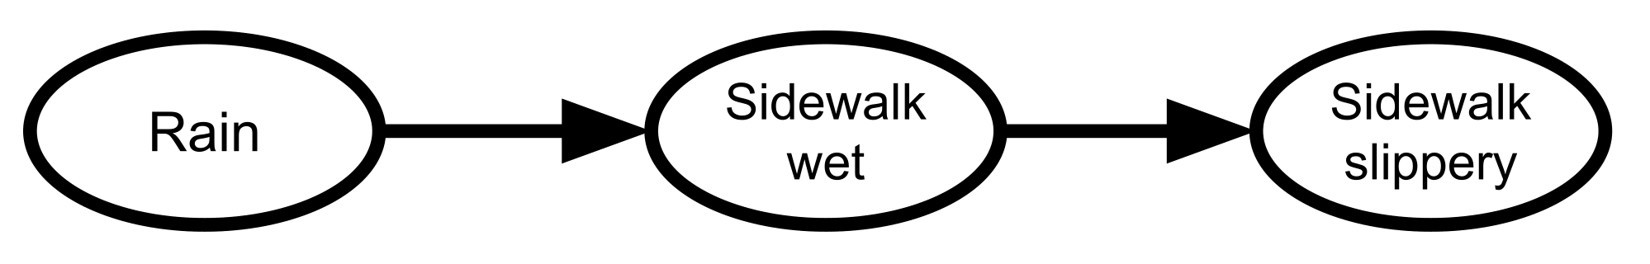
\includegraphics[scale=0.25]{Rationality20From20AI20to20Zombies2020Eliezer20Yudkowsky-img44.jpg}
 }

{
\ \ \ ~}

{
\ \ \ From this we can infer---or, in a Bayes net, rigorously calculate
in probabilities---that when the sidewalk is slippery, it probably
rained; but if we already know that the sidewalk is wet, learning that
the sidewalk is slippery tells us nothing more about whether it
rained.}

{
\ \ \ Why is fire hot and bright when it burns?}

{
\ \ \ ~}

{
\ \ \  

\includegraphics[scale=0.25]{Rationality20From20AI20to20Zombies2020Eliezer20Yudkowsky-img45.jpg}
 }

{
\ \ \ ~}

{
\ \ \ It \textit{feels} like an explanation. It's
\textit{represented} using the same cognitive data format. But the
human mind does not automatically detect when a cause has an
unconstraining arrow to its effect. Worse, thanks to hindsight bias, it
may feel like the cause constrains the effect, when it was merely
fitted to the effect.}

{
\ \ \ Interestingly, our modern understanding of probabilistic reasoning
about causality can describe precisely what the phlogiston theorists
were doing wrong. One of the primary inspirations for Bayesian networks
was noticing the problem of double-counting evidence if inference
resonates between an effect and a cause. For example,
let's say that I get a bit of unreliable information
that the sidewalk is wet. This should make me think
it's more likely to be raining. But, if
it's more likely to be raining, doesn't
that make it more likely that the sidewalk is wet? And
wouldn't \textit{that} make it more likely that the
sidewalk is slippery? But if the sidewalk is slippery,
it's probably wet; and then I should again raise my
probability that it's raining .~.~.}

{
\ \ \ Judea Pearl uses the metaphor of an algorithm for counting
soldiers in a line.\textsuperscript{1} Suppose you're
in the line, and you see two soldiers next to you, one in front and one
in back. That's three soldiers, including you. So you
ask the soldier behind you, ``How many soldiers do
\textit{you} see?'' They look around and say,
``Three.'' So that's
a total of six soldiers. This, obviously, is \textit{not} how to do
it.}

{
\ \ \ A smarter way is to ask the soldier in front of you,
``How many soldiers forward of
you?'' and the soldier in back,
``How many soldiers backward of
you?'' The question ``How many
soldiers forward?'' can be passed on as a message
without confusion. If I'm at the front of the line, I
pass the message ``1 soldier
forward,'' for myself. The person directly in back of
me gets the message ``1 soldier
forward,'' and passes on the message
``2 soldiers forward'' to the
soldier behind them. At the same time, each soldier is also getting the
message ``N soldiers backward'' from
the soldier behind them, and passing it on as ``N + 1
soldiers backward'' to the soldier in front of them.
How many soldiers in total? Add the two numbers you receive, plus one
for yourself: that is the total number of soldiers in line.}

{
\ \ \ The key idea is that every soldier must \textit{separately} track
the two messages, the forward-message and backward-message, and add
them together only at the end. You never add any soldiers from the
backward-message you receive to the forward-message you pass back.
Indeed, the total number of soldiers is never passed as a message---no
one ever says it aloud.}

{
\ \ \ An analogous principle operates in rigorous probabilistic
reasoning about causality. If you learn something about whether
it's raining, from some source \textit{other} than
observing the sidewalk to be wet, this will send a forward-message from
Rain to Sidewalk wet and raise our expectation of the sidewalk being
wet. If you observe the sidewalk to be wet, this sends a
backward-message to our belief that it is raining, and this message
propagates from Rain to all neighboring nodes \textit{except} the
Sidewalk wet node. We count each piece of evidence exactly once; no
update message ever ``bounces'' back
and forth. The exact algorithm may be found in Judea
Pearl's classic \textit{Probabilistic Reasoning in
Intelligent Systems: Networks of Plausible Inference}.}

{
\ \ \ So what went wrong in phlogiston theory? When we observe that fire
is hot, the Fire node can send a backward-evidence to the Phlogiston
node, leading us to update our beliefs about phlogiston. But if so, we
can't count this as a successful forward-prediction of
phlogiston theory. The message should go in only one direction, and not
bounce back.}

{
\ \ \ Alas, human beings do not use a rigorous algorithm for updating
belief networks. We learn about parent nodes from observing children,
and predict child nodes from beliefs about parents. But we
don't keep rigorously separate books for the
backward-message and forward-message. We just remember that phlogiston
is hot, which \textit{causes} fire to be hot. So it seems like
phlogiston theory predicts the hotness of fire. Or, worse, it just
feels like \textit{phlogiston makes the fire hot.}}

{
\ \ \ Until you notice that no \textit{advance} predictions are being
made, the non-constraining causal node is not labeled
``fake.'' It's
represented the same way as any other node in your belief network. It
feels like a fact, like all the other facts you know:
\textit{Phlogiston makes the fire hot.}}

{
\ \ \ A properly designed AI would notice the problem instantly. This
wouldn't even require special-purpose code, just
correct bookkeeping of the belief network. (Sadly, we humans
can't rewrite our own code, the way a properly designed
AI could.)}

{
\ \ \ Speaking of ``hindsight bias''
is just the nontechnical way of saying that humans do not rigorously
separate forward and backward messages, allowing forward messages to be
contaminated by backward ones.}

{
\ \ \ Those who long ago went down the path of phlogiston were not
trying to be fools. No scientist deliberately wants to get stuck in a
blind alley. Are there any fake explanations in \textit{your} mind? If
there are, I guarantee they're not labeled
``fake explanation,'' so polling
your thoughts for the ``fake''
keyword will not turn them up.}

{
\ \ \ Thanks to hindsight bias, it's also not enough to
check how well your theory
``predicts'' facts you already know.
You've got to predict for tomorrow, not yesterday.
It's the only way a messy human mind can be guaranteed
of sending a pure forward message.}

{\centering
\ \ \ \ ~
\par}

{\centering
\ \ \ *
\par}


\bigskip

{
\ \ \ 1. Judea Pearl, \textit{Probabilistic Reasoning in Intelligent
Systems: Networks of Plausible Inference} (San Mateo, CA: Morgan
Kaufmann, 1988).}

\mysection{Semantic Stopsigns}

{
\ \ \ \textit{And the child asked:}}

{
\ \ \ Q: Where did this rock come from?}

{
\ \ \ A: I chipped it off the big boulder, at the center of the
village.}

{
\ \ \ Q: Where did the boulder come from?}

{
\ \ \ A: It probably rolled off the huge mountain that towers over our
village.}

{
\ \ \ Q: Where did the mountain come from?}

{
\ \ \ A: The same place as all stone: it is the bones of Ymir, the
primordial giant.}

{
\ \ \ Q: Where did the primordial giant, Ymir, come from?}

{
\ \ \ A: From the great abyss, Ginnungagap.}

{
\ \ \ Q: Where did the great abyss, Ginnungagap, come from?}

{
\ \ \ A: Never ask that question.}

{
\ \ \ Consider the seeming paradox of the First Cause. Science has
traced events back to the Big Bang, but why did the Big Bang happen?
It's all well and good to say that the zero of time
begins at the Big Bang---that there is nothing before the Big Bang in
the ordinary flow of minutes and hours. But saying this presumes our
physical law, which itself appears highly structured; it calls out for
explanation. Where did the physical laws come from? You could say that
we're all a computer simulation, but then the computer
simulation is running on some other world's laws of
physics---where did \textit{those} laws of physics come from?}

{
\ \ \ At this point, some people say,
``God!''}

{
\ \ \ What could possibly make anyone, even a highly religious person,
think this even \textit{helped} answer the paradox of the First Cause?
Why wouldn't you automatically ask,
``Where did God come from?'' Saying
``God is uncaused'' or
``God created Himself'' leaves us in
exactly the same position as ``Time began with the Big
Bang.'' We just ask why the whole metasystem exists
in the first place, or why some events but not others are allowed to be
uncaused.}

{
\ \ \ My purpose here is not to discuss the seeming paradox of the First
Cause, but to ask why anyone would think
``God!'' \textit{could} resolve the
paradox. Saying ``God!'' is a way of
belonging to a tribe, which gives people a motive to say it as often as
possible---some people even say it for questions like
``Why did this hurricane strike New
Orleans?'' Even so, you'd hope people
would notice that on the \textit{particular} puzzle of the First Cause,
saying ``God!''
doesn't help. It doesn't make the
paradox seem any less paradoxical \textit{even if true.} How could
anyone \textit{not} notice this?}

{
\ \ \ Jonathan Wallace suggested that
``God!'' functions as a
\textit{semantic stopsign}{}---that it isn't a
propositional assertion, so much as a cognitive traffic signal: do not
think past this point. Saying
``God!'' doesn't so
much resolve the paradox, as put up a cognitive traffic signal to halt
the obvious continuation of the question-and-answer chain.}

{
\ \ \ Of course \textit{you'd} never do that, being a
good and proper atheist, right? But
``God!'' isn't the
\textit{only} semantic stopsign, just the obvious first example.}

{
\ \ \ The transhuman technologies---molecular nanotechnology, advanced
biotech, genetech, Artificial Intelligence, et cetera---pose tough
policy questions. What kind of role, if any, should a government take
in supervising a parent's choice of genes for their
child? Could parents deliberately choose genes for schizophrenia? If
enhancing a child's intelligence is expensive, should
governments help ensure access, to prevent the emergence of a cognitive
elite? You can propose various institutions to answer these policy
questions---for example, that private charities should provide
financial aid for intelligence enhancement---but the obvious next
question is, ``Will this institution be
effective?'' If we rely on product liability lawsuits
to prevent corporations from building harmful nanotech, will that
really \textit{work}?}

{
\ \ \ I know someone whose answer to every one of these questions is
``Liberal democracy!''
That's it. That's his answer. If you
ask the obvious question of ``How well have liberal
democracies performed, historically, on problems this
tricky?'' or ``What if liberal
democracy does something stupid?'' then
you're an autocrat, or libertopian, or otherwise a very
very bad person. No one is allowed to question democracy.}

{
\ \ \ I once called this kind of thinking ``the divine
right of democracy.'' But it is more precise to say
that ``Democracy!'' functioned for
him as a semantic stopsign. If anyone had said to him
``Turn it over to the Coca-Cola
corporation!,'' he would have asked the obvious next
questions: ``Why? What will the Coca-Cola corporation
do about it? Why should we trust them? Have they done well in the past
on equally tricky problems?''}

{
\ \ \ Or suppose that someone says ``Mexican-Americans
are plotting to remove all the oxygen in Earth's
atmosphere.'' You'd probably ask,
``Why would they do \textit{that}?
Don't Mexican-Americans have to breathe too? Do
Mexican-Americans even function as a unified
conspiracy?'' If you don't ask these
obvious next questions when someone says,
``Corporations are plotting to remove
Earth's oxygen,'' then
``Corporations!'' functions for you
as a semantic stopsign.}

{
\ \ \ Be careful here not to create a new generic counterargument
against things you don't like---``Oh,
it's just a stopsign!'' No word is a
stopsign of itself; the question is whether a word has that effect on a
particular person. Having strong emotions about something
doesn't qualify it as a stopsign. I'm
not exactly fond of terrorists or fearful of private property; that
doesn't mean
``Terrorists!'' or
``Capitalism!'' are cognitive
traffic signals unto me. (The word
``intelligence'' did once have that
effect on me, though no longer.) What distinguishes a semantic stopsign
is \textit{failure to consider the obvious next question.}}

{\centering
\ \ \ \ ~
\par}

{\centering
\ \ \ *
\par}

\mysection{Mysterious Answers to Mysterious Questions}

{
\ \ \ Imagine looking at your hand, and knowing nothing of cells,
nothing of biochemistry, nothing of DNA. You've learned
some anatomy from dissection, so you know your hand contains muscles;
but you don't know why muscles move instead of lying
there like clay. Your hand is just .~.~. stuff .~.~. and for some
reason it moves under your direction. Is this not magic?}

{
\ \ \ The animal body does not act as a thermodynamic engine .~.~.
consciousness teaches every individual that they are, to some extent,
subject to the direction of his will. It appears therefore that
animated creatures have the power of immediately applying to certain
moving particles of matter within their bodies, forces by which the
motions of these particles are directed to produce derived mechanical
effects .~.~. The influence of animal or vegetable life on matter is
infinitely beyond the range of any scientific inquiry hitherto entered
on. Its power of directing the motions of moving particles, in the
demonstrated daily miracle of our human free-will, and in the growth of
generation after generation of plants from a single seed, are
infinitely different from any possible result of the fortuitous
concurrence of atoms .~.~. Modern biologists were coming once more to
the acceptance of something and that was a vital principle.}

{\raggedleft
\ \ \ {}---Lord Kelvin\textsuperscript{1}
\par}


\bigskip

{
\ \ \ This was the theory of \textit{vitalism}; that the mysterious
difference between living matter and non-living matter was explained by
an \textit{élan vital} or \textit{vis vitalis}. \textit{élan vital}
infused living matter and caused it to move as consciously directed.
\textit{élan vital} participated in chemical transformations which no
mere non-living particles could undergo---Wöhler's
later synthesis of urea, a component of urine, was a major blow to the
vitalistic theory because it showed that mere \textit{chemistry} could
duplicate a product of biology.}

{
\ \ \ Calling ``élan vital'' an
explanation, even a fake explanation like phlogiston, is probably
giving it too much credit. It functioned primarily as a
curiosity-stopper. You said ``Why?''
and the answer was ``Élan vital!''}

{
\ \ \ When you say ``Élan vital!,''
it \textit{feels} like you know why your hand moves. You have a little
causal diagram in your head that says:}

{
\ \ \ ~}

{
\ \ \  

\includegraphics[scale=0.25]{Rationality20From20AI20to20Zombies2020Eliezer20Yudkowsky-img48.jpg}
 }

{
\ \ \ ~}

{
\ \ \ But actually you know nothing you didn't know
before. You don't know, say, whether your hand will
generate heat or absorb heat, unless you have observed the fact
already; if not, you won't be able to predict it in
advance. Your curiosity feels sated, but it hasn't been
fed. Since you can say ``Why? Élan
vital!'' to any possible observation, it is equally
good at explaining all outcomes, a disguised hypothesis of maximum
entropy, et cetera.}

{
\ \ \ But the greater lesson lies in the vitalists'
reverence for the \textit{élan vital}, their eagerness to pronounce it
a mystery beyond all science. Meeting the great dragon Unknown, the
vitalists did not draw their swords to do battle, but bowed their necks
in submission. They took pride in their ignorance, made biology into a
\textit{sacred} mystery, and thereby became loath to relinquish their
ignorance when evidence came knocking.}

{
\ \ \ The Secret of Life was \textit{infinitely beyond the reach of
science!} Not just a \textit{little} beyond, mind you, but
\textit{infinitely} beyond! Lord Kelvin sure did get a tremendous
emotional kick out of \textit{not knowing something.}}

{
\ \ \ But ignorance exists in the map, not in the territory. If I am
ignorant about a phenomenon, that is a fact about my own state of mind,
not a fact about the phenomenon itself. A phenomenon can \textit{seem}
mysterious to some particular person. There are no phenomena which are
mysterious of themselves. To worship a phenomenon because it seems so
wonderfully mysterious is to worship your own ignorance.}

{
\ \ \ Vitalism shared with phlogiston the error of \textit{encapsulating
the mystery as a substance.} Fire was mysterious, and the phlogiston
theory encapsulated the mystery in a mysterious substance called
``phlogiston.'' Life was a sacred
mystery, and vitalism encapsulated the sacred mystery in a mysterious
substance called ``élan vital.''
Neither answer helped concentrate the model's
probability density---make some outcomes easier to explain than others.
The ``explanation'' just wrapped up
the question as a small, hard, opaque black ball.}

{
\ \ \ In a comedy written by Moliére, a physician explains the power of
a soporific by saying that it contains a ``dormitive
potency.'' Same principle. It is a failure of human
psychology that, faced with a mysterious phenomenon, we more readily
postulate mysterious inherent substances than complex underlying
processes.}

{
\ \ \ But the deeper failure is supposing that an \textit{answer} can be
mysterious. If a phenomenon feels mysterious, that is a fact about our
state of knowledge, not a fact about the phenomenon itself. The
vitalists saw a mysterious gap in their knowledge, and postulated a
mysterious stuff that plugged the gap. In doing so, they mixed up the
map with the territory. All confusion and bewilderment exist in the
mind, not in encapsulated substances.}

{
\ \ \ This is the ultimate and fully general explanation for why, again
and again in humanity's history, people are shocked to
discover that an incredibly mysterious question has a non-mysterious
answer. Mystery is a property of questions, not answers.}

{
\ \ \ Therefore I call theories such as vitalism \textit{mysterious
answers to mysterious questions}.}

{
\ \ \ These are the signs of mysterious answers to mysterious
questions:}

{
\ \ \ First, the explanation acts as a curiosity-stopper rather than an
anticipation-controller.}

{
\ \ \ Second, the hypothesis has no moving parts---the model is not a
specific complex mechanism, but a blankly solid substance or force. The
mysterious substance or mysterious force may be said to be here or
there, to cause this or that; but the reason why the mysterious force
behaves thus is wrapped in a blank unity.}

{
\ \ \ Third, those who proffer the explanation cherish their ignorance;
they speak proudly of how the phenomenon defeats ordinary science or is
unlike merely mundane phenomena.}

{
\ \ \ Fourth, \textit{even after the answer is given, the phenomenon is
still a mystery} and possesses the same quality of wonderful
inexplicability that it had at the start.}

{\centering
\ \ \ \ ~
\par}

{\centering
\ \ \ *
\par}


\bigskip

{
\ \ \ 1. Silvanus Phillips Thompson, \textit{The Life of Lord Kelvin}
(American Mathematical Society, 2005).}

\mysection{The Futility of Emergence}

{
\ \ \ The failures of phlogiston and vitalism are historical hindsight.
Dare I step out on a limb, and name some \textit{current} theory which
I deem analogously flawed? }

{
\ \ \ I name \textit{emergence} or \textit{emergent
phenomena}{}---usually defined as the study of systems whose high-level
behaviors arise or ``emerge'' from
the interaction of many low-level elements. (Wikipedia:
``The way complex systems and patterns arise out of a
multiplicity of relatively simple interactions.'')
Taken literally, that description fits every phenomenon in our universe
above the level of individual quarks, which is part of the problem.
Imagine pointing to a market crash and saying
``It's not a
quark!'' Does that feel like an explanation? No? Then
neither should saying ``It's an
emergent phenomenon!''}

{
\ \ \ It's the noun
``emergence'' that I protest, rather
than the verb ``emerges from.''
There's nothing wrong with saying ``X
emerges from Y,'' where Y is some specific, detailed
model with internal moving parts. ``Arises
from'' is another legitimate phrase that means
exactly the same thing: Gravity arises from the curvature of spacetime,
according to the specific mathematical model of General Relativity.
Chemistry arises from interactions between atoms, according to the
specific model of quantum electrodynamics.}

{
\ \ \ Now suppose I should say that gravity is explained by
``arisence'' or that chemistry is an
``arising phenomenon,'' and claim
that as my explanation.}

{
\ \ \ The phrase ``emerges from'' is
acceptable, just like ``arises
from'' or ``is caused
by'' are acceptable, if the phrase precedes some
specific model to be judged on its own merits.}

{
\ \ \ However, this is \textit{not} the way
``emergence'' is commonly used.
``Emergence'' is commonly used as an
explanation in its own right.}

{
\ \ \ I have lost track of how many times I have heard people say,
``Intelligence is an emergent
phenomenon!'' as if that explained intelligence. This
usage fits all the checklist items for a mysterious answer to a
mysterious question. What do you know, after you have said that
intelligence is ``emergent''? You
can make no new predictions. You do not know anything about the
behavior of real-world minds that you did not know before. It feels
like you believe a new fact, but you don't anticipate
any different outcomes. Your curiosity feels sated, but it has not been
fed. The hypothesis has no moving parts---there's no
detailed internal model to manipulate. Those who proffer the hypothesis
of ``emergence'' confess their
ignorance of the internals, and take pride in it; they contrast the
science of ``emergence'' to other
sciences merely mundane.}

{
\ \ \ And even after the answer of ``Why?
Emergence!'' is given, \textit{the phenomenon is
still a mystery} and possesses the same sacred impenetrability it had
at the start.}

{
\ \ \ A fun exercise is to eliminate the adjective
``emergent'' from any sentence in
which it appears, and see if the sentence says anything different:}

{
\ \ \ \textit{Before:} Human intelligence is an emergent product of
neurons firing.}

{
\ \ \ \textit{After:} Human intelligence is a product of neurons
firing.}

{
\ \ \ \textit{Before:} The behavior of the ant colony is the emergent
outcome of the interactions of many individual ants.}

{
\ \ \ \textit{After:} The behavior of the ant colony is the outcome of
the interactions of many individual ants.}

{
\ \ \ \textit{Even better:} A colony is made of ants. We can
successfully predict some aspects of colony behavior using models that
include only individual ants, without any global colony variables,
showing that we understand how those colony behaviors arise from ant
behaviors.}

{
\ \ \ Another fun exercise is to replace the word
``emergent'' with the old word, the
explanation that people had to use before emergence was invented:}

{
\ \ \ \textit{Before:} Life is an emergent phenomenon.}

{
\ \ \ \textit{After:} Life is a magical phenomenon.}

{
\ \ \ \textit{Before:} Human intelligence is an emergent product of
neurons firing.}

{
\ \ \ \textit{After:} Human intelligence is a magical product of neurons
firing.}

{
\ \ \ Does not each statement convey exactly the same amount of
knowledge about the phenomenon's behavior? Does not
each hypothesis fit exactly the same set of outcomes?}

{
\ \ \ ``Emergence'' has become very
popular, just as saying ``magic''
used to be very popular.
``Emergence'' has the same deep
appeal to human psychology, for the same reason.
``Emergence'' is such a wonderfully
easy explanation, and it feels good to say it; it gives you a sacred
mystery to worship. Emergence is popular \textit{because} it is the
junk food of curiosity. You can explain anything using emergence, and
so people do just that; for it feels so wonderful to explain things.
Humans are still humans, even if they've taken a few
science classes in college. Once they find a way to escape the shackles
of settled science, they get up to the same shenanigans as their
ancestors---dressed up in the literary genre of
``science,'' but humans are still
humans, and human psychology is still human psychology.}

{\centering
\ \ \ \ ~
\par}

{\centering
\ \ \ *
\par}

\mysection{Say Not ``Complexity''}

{
\ \ \ Once upon a time .~.~. }

{
\ \ \ This is a story from when I first met Marcello, with whom I would
later work for a year on AI theory; but at this point I had not yet
accepted him as my apprentice. I knew that he competed at the national
level in mathematical and computing olympiads, which sufficed to
attract my attention for a closer look; but I didn't
know yet if he could learn to think about AI.}

{
\ \ \ I had asked Marcello to say how he thought an AI might discover
how to solve a Rubik's Cube. Not in a preprogrammed
way, which is trivial, but rather how the AI itself might figure out
the laws of the Rubik universe and reason out how to exploit them. How
would an AI \textit{invent for itself} the concept of an
``operator,'' or
``macro,'' which is the key to
solving the Rubik's Cube?}

{
\ \ \ At some point in this discussion, Marcello said:
``Well, I think the AI needs complexity to do X, and
complexity to do Y---''}

{
\ \ \ And I said, ``Don't say
`\textit{complexity.}'''}

{
\ \ \ Marcello said, ``Why not?''}

{
\ \ \ I said, ``Complexity should never be a goal in
itself. You may need to use a particular algorithm that adds some
amount of complexity, but complexity for the sake of complexity just
makes things harder.'' (I was thinking of all the
people whom I had heard advocating that the Internet would
``wake up'' and become an AI when it
became ``sufficiently complex.'')}

{
\ \ \ And Marcello said, ``But there's
got to be \textit{some} amount of complexity that does
it.''}

{
\ \ \ I closed my eyes briefly, and tried to think of how to explain it
all in words. To me, saying
``complexity'' simply \textit{felt}
like the wrong move in the AI dance. No one can think fast enough to
deliberate, in words, about each sentence of their stream of
consciousness; for that would require an infinite recursion. We think
in words, but our stream of consciousness is steered below the level of
words, by the trained-in remnants of past insights and harsh experience
.~.~.}

{
\ \ \ I said, ``Did you read A Technical Explanation of
Technical Explanation?''}

{
\ \ \ ``Yes,'' said Marcello.}

{
\ \ \ ``Okay,'' I said.
``Saying `complexity'
doesn't concentrate your probability
mass.''}

{
\ \ \ ``Oh,'' Marcello said,
``like `emergence.'
Huh. So .~.~. now I've got to think about how X might
actually happen .~.~.''}

{
\ \ \ That was when I thought to myself,
``\textit{Maybe }\textbf{\textit{this}}\textit{ one is
teachable.}''}

{
\ \ \ Complexity is not a useless concept. It has mathematical
definitions attached to it, such as Kolmogorov complexity and
Vapnik-Chervonenkis complexity. Even on an intuitive level, complexity
is often worth thinking about---you have to judge the complexity of a
hypothesis and decide if it's ``too
complicated'' given the supporting evidence, or look
at a design and try to make it simpler.}

{
\ \ \ But concepts are not useful or useless of themselves. Only
\textit{usages} are correct or incorrect. In the step Marcello was
trying to take in the dance, he was trying to explain something for
free, get something for nothing. It is an extremely common misstep, at
least in my field. You can join a discussion on Artificial General
Intelligence and watch people doing the same thing, left and right,
over and over again---constantly skipping over things they
don't understand, without realizing
that's what they're doing.}

{
\ \ \ In an eyeblink it happens: putting a non-controlling causal node
behind something mysterious, a causal node that feels like an
explanation but isn't. The mistake takes place below
the level of words. It requires no special character flaw; it is how
human beings think by default, how they have thought since the ancient
times.}

{
\ \ \ What you must avoid is \textit{skipping over the mysterious part};
you must linger at the mystery to confront it directly. There are many
words that can skip over mysteries, and some of them would be
legitimate in other
contexts---``complexity,'' for
example. But the essential mistake is that \textit{skip-over},
regardless of what causal node goes behind it. The skip-over is not a
thought, but a microthought. You have to pay close attention to catch
yourself at it. And when you train yourself to avoid skipping, it will
become a matter of instinct, not verbal reasoning. You have to
\textit{feel} which parts of your map are still blank, and more
importantly, pay attention to that feeling.}

{
\ \ \ I suspect that in academia there is a huge pressure to sweep
problems under the rug so that you can present a paper with the
appearance of completeness. You'll get more kudos for a
seemingly complete model that includes some ``emergent
phenomena,'' versus an explicitly incomplete map
where the label says ``I got no clue how this part
works'' or ``then a miracle
occurs.'' A journal may not even accept the latter
paper, since who knows but that the unknown steps are really where
everything interesting happens? And yes, it sometimes happens that all
the non-magical parts of your map turn out to also be non-important.
That's the price you sometimes pay, for entering into
terra incognita and trying to solve problems \textit{incrementally.}
But that makes it even \textit{more} important to \textit{know} when
you aren't finished yet. Mostly, people
don't dare to enter terra incognita at all, for the
deadly fear of wasting their time.}

{
\ \ \ And if you're working on a revolutionary AI
startup, there is an even huger pressure to sweep problems under the
rug; or you will have to admit to yourself that you
don't know how to build an AI yet, and your current
life plans will come crashing down in ruins around your ears. But
perhaps I am over-explaining, since skip-over happens by default in
humans; if you're looking for examples, just watch
people discussing religion or philosophy or spirituality or any science
in which they were not professionally trained.}

{
\ \ \ Marcello and I developed a convention in our AI work: when we ran
into something we didn't understand, which was often,
we would say ``magic''---as in,
``X magically does Y''---to remind
ourselves that \textit{here was an unsolved problem, a gap in our
understanding.} It is far better to say
``magic,'' than
``complexity'' or
``emergence''; the latter words
create an illusion of understanding. Wiser to say
``magic,'' and leave yourself a
placeholder, a reminder of work you will have to do later.}

{\centering
\ \ \ \ ~
\par}

{\centering
\ \ \ *
\par}

\mysection{Positive Bias: Look into the Dark}

{
\ \ \ I am teaching a class, and I write upon the blackboard three
numbers: 2-4-6. ``I am thinking of a
rule,'' I say, ``which governs
sequences of three numbers. The sequence 2-4-6, as it so happens, obeys
this rule. Each of you will find, on your desk, a pile of index cards.
Write down a sequence of three numbers on a card, and
I'll mark it `Yes' for
fits the rule, or `No' for not fitting
the rule. Then you can write down another set of three numbers and ask
whether it fits again, and so on. When you're confident
that you know the rule, write down the rule on a card. You can test as
many triplets as you like.'' }

{
\ \ \ Here's the record of one student's
guesses:\newline
}

{\centering
\ \ \ 4-6-2 ~No\newline
 4-6-8 ~Yes\newline
 10-12-14 ~Yes
\par}


\bigskip

{
\ \ \ At this point the student wrote down their guess at the rule. What
do \textit{you} think the rule is? Would you have wanted to test
another triplet, and if so, what would it be? Take a moment to think
before continuing. }

{
\ \ \ The challenge above is based on a classic experiment due to Peter
Wason, the 2-4-6 task. Although subjects given this task typically
expressed high confidence in their guesses, only 21\% of the subjects
successfully guessed the experimenter's real rule, and
replications since then have continued to show success rates of around
20\%.\textsuperscript{1}}

{
\ \ \ The study was called ``On the failure to
eliminate hypotheses in a conceptual task.'' Subjects
who attempt the 2-4-6 task usually try to generate \textit{positive}
examples, rather than \textit{negative} examples---they apply the
hypothetical rule to generate a representative instance, and see if it
is labeled ``Yes.''}

{
\ \ \ Thus, someone who forms the hypothesis ``numbers
increasing by two'' will test the triplet 8-10-12,
hear that it fits, and confidently announce the rule. Someone who forms
the hypothesis X-2X-3X will test the triplet 3-6-9, discover that it
fits, and then announce that rule.}

{
\ \ \ In every case the actual rule is the same: the three numbers must
be in ascending order.}

{
\ \ \ But to discover this, you would have to generate triplets that
\textit{shouldn't} fit, such as 20-23-26, and see if
they are labeled ``No.'' Which
people tend not to do, in this experiment. In some cases, subjects
devise, ``test,'' and announce rules
far more complicated than the actual answer.}

{
\ \ \ This cognitive phenomenon is usually lumped in with
``confirmation bias.'' However, it
seems to me that the phenomenon of trying to test \textit{positive}
rather than \textit{negative} examples, ought to be distinguished from
the phenomenon of trying to preserve the belief you started with.
``Positive bias'' is sometimes used
as a synonym for ``confirmation
bias,'' and fits this particular flaw much better.}

{
\ \ \ It once seemed that phlogiston theory could explain a flame going
out in an enclosed box (the air became saturated with phlogiston and no
more could be released), but phlogiston theory could just as well have
explained the flame \textit{not} going out. To notice this, you have to
search for negative examples instead of positive examples, look into
zero instead of one; which goes against the grain of what experiment
has shown to be human instinct.}

{
\ \ \ For by instinct, we human beings only live in half the world.}

{
\ \ \ One may be lectured on positive bias for days, and yet overlook it
in-the-moment. Positive bias is not something we do as a matter of
logic, or even as a matter of emotional attachment. The 2-4-6 task is
``cold,'' logical, not affectively
``hot.'' And yet the mistake is
sub-verbal, on the level of imagery, of instinctive reactions. Because
the problem doesn't arise from following a deliberate
rule that says ``Only think about positive
examples,'' it can't be solved just
by knowing verbally that ``We ought to think about
both positive and negative examples.'' Which example
automatically pops into your head? You have to learn, wordlessly, to
zag instead of zig. You have to learn to flinch toward the zero,
instead of away from it.}

{
\ \ \ I have been writing for quite some time now on the notion that the
strength of a hypothesis is what it \textit{can't}
explain, not what it \textit{can}{}---if you are equally good at
explaining any outcome, you have zero knowledge. So to spot an
explanation that isn't helpful, it's
not enough to think of what it does explain very well---you also have
to search for results it \textit{couldn't} explain, and
this is the true strength of the theory.}

{
\ \ \ So I said all this, and then I challenged the usefulness of
``emergence'' as a concept. One
commenter cited superconductivity and ferromagnetism as examples of
emergence. I replied that non-superconductivity and non-ferromagnetism
were also examples of emergence, which was the problem. But be it far
from me to criticize the commenter! Despite having read extensively on
``confirmation bias,'' I
didn't spot the
``gotcha'' in the 2-4-6 task the
first time I read about it. It's a subverbal
blink-reaction that has to be retrained. I'm still
working on it myself.}

{
\ \ \ So much of a rationalist's skill is below the
level of words. It makes for challenging work in trying to convey the
Art through words. People will agree with you, but then, in the next
sentence, do something subdeliberative that goes in the opposite
direction. Not that I'm complaining! A major reason
I'm writing this is to observe what my words
\textit{haven't} conveyed.}

{
\ \ \ Are you searching for positive examples of positive bias right
now, or sparing a fraction of your search on what positive bias should
lead you to \textit{not} see? Did you look toward light or darkness?}

{\centering
\ \ \ \ ~
\par}

{\centering
\ \ \ *
\par}


\bigskip

{
\ \ \ 1. Peter Cathcart Wason, ``On the Failure to
Eliminate Hypotheses in a Conceptual Task,''
\textit{Quarterly Journal of Experimental Psychology} 12, no. 3 (1960):
129--140, doi:10.1080/17470216008416717.}

\mysection{Lawful Uncertainty}

{
\ \ \ In \textit{Rational Choice in an Uncertain World}, Robyn Dawes
describes an experiment by Tversky:\textsuperscript{1,2}}

{
\ \ \ Many psychological experiments were conducted in the late 1950s
and early 1960s in which subjects were asked to predict the outcome of
an event that had a random component but yet had base-rate
predictability---for example, subjects were asked to predict whether
the next card the experimenter turned over would be red or blue in a
context in which 70\% of the cards were blue, but in which the sequence
of red and blue cards was totally random.}

{
\ \ \ In such a situation, the strategy that will yield the highest
proportion of success is to predict the more common event. For example,
if 70\% of the cards are blue, then predicting blue on every trial
yields a 70\% success rate.}

{
\ \ \ What subjects tended to do instead, however, was match
probabilities---that is, predict the more probable event with the
relative frequency with which it occurred. For example, subjects tended
to predict 70\% of the time that the blue card would occur and 30\% of
the time that the red card would occur. Such a strategy yields a 58\%
success rate, because the subjects are correct 70\% of the time when
the blue card occurs (which happens with probability .70) and 30\% of
the time when the red card occurs (which happens with probability .30);
(.70 {\texttimes} .70) + (.30 {\texttimes} .30) = .58.}

{
\ \ \ In fact, subjects predict the more frequent event with a slightly
higher probability than that with which it occurs, but do not come
close to predicting its occurrence 100\% of the time, even when they
are paid for the accuracy of their predictions .~.~. For example,
subjects who were paid a nickel for each correct prediction over a
thousand trials .~.~. predicted [the more common event] 76\% of the
time.}

{
\ \ \ Do not think that this experiment is about a minor flaw in
gambling strategies. It compactly illustrates the most important idea
in all of rationality.}

{
\ \ \ Subjects just keep guessing red, as if they think they have some
way of predicting the random sequence. Of this experiment Dawes goes on
to say, ``Despite feedback through a thousand trials,
subjects cannot bring themselves to believe that the situation is one
in which they \textit{cannot} predict.''}

{
\ \ \ But the error must go deeper than that. Even if subjects
\textit{think} they've come up with a hypothesis, they
don't have to \textit{actually bet} on that prediction
in order to test their hypothesis. They can say, ``Now
if \textit{this} hypothesis is correct, the next card will be
red''---and then just bet on blue. They can pick blue
each time, accumulating as many nickels as they can, while mentally
noting their private guesses for any patterns they thought they
spotted. If their predictions come out right, \textit{then} they can
switch to the newly discovered sequence.}

{
\ \ \ I wouldn't fault a subject for continuing to
invent hypotheses---how could they know the sequence is truly beyond
their ability to predict? But I would fault a subject for
\textit{betting on the guesses}, when this wasn't
necessary to gather information, and literally \textit{hundreds} of
earlier guesses had been disconfirmed.}

{
\ \ \ Can even a human be \textit{that} overconfident?}

{
\ \ \ I would suspect that something simpler is going on---that the
all-blue strategy \textit{just didn't occur} to the
subjects.}

{
\ \ \ People see a mix of mostly blue cards with some red, and suppose
that the optimal betting strategy must be a mix of mostly blue cards
with some red.}

{
\ \ \ It is a \textit{counterintuitive} idea that, given incomplete
information, \textit{the optimal betting strategy does not resemble a
typical sequence of cards}.}

{
\ \ \ It is a \textit{counterintuitive} idea that the optimal strategy
is to behave lawfully, even in an environment that has random
elements.}

{
\ \ \ It seems like your behavior ought to be unpredictable, just like
the environment---but no! \textit{A random key does not open a random
lock just because they are ``both
random.''}}

{
\ \ \ You don't fight fire with fire; you fight fire
with water. But this thought involves an extra step, a new concept not
directly activated by the problem statement, and so
it's not the first idea that comes to mind.}

{
\ \ \ In the dilemma of the blue and red cards, our partial knowledge
tells us---on each and every round---that the best bet is blue. This
advice of our partial knowledge is the same on each and every round. If
30\% of the time we go against our partial knowledge and bet on red
instead, then we will do worse thereby---because now
we're being outright stupid, betting on what we know is
the less probable outcome.}

{
\ \ \ If you bet on red every round, you would do as badly as you could
possibly do; you would be 100\% stupid. If you bet on red 30\% of the
time, faced with 30\% red cards, then you're making
yourself 30\% stupid.}

{
\ \ \ When your knowledge is incomplete---meaning that the world will
seem to you to have an element of randomness---randomizing your actions
doesn't solve the problem. Randomizing your actions
takes you further from the target, not closer. In a world already
foggy, throwing away your intelligence just makes things worse.}

{
\ \ \ It is a \textit{counterintuitive} idea that the optimal strategy
can be to \textit{think lawfully, even under conditions of
uncertainty}.}

{
\ \ \ And so there are not many rationalists, for most who perceive a
chaotic world will try to fight chaos with chaos. You have to take an
extra step, and think of something that doesn't pop
right into your mind, in order to imagine fighting fire with something
that is not itself fire.}

{
\ \ \ You have heard the unenlightened ones say,
``Rationality works fine for dealing with rational
people, but the world isn't
rational.'' But \textit{faced with an irrational
opponent, throwing away your own reason is not going to help you}.
There are lawful forms of thought that still generate the best
response, even when faced with an opponent who breaks those laws.
Decision theory does \textit{not} burst into flames and die when faced
with an opponent who disobeys decision theory.}

{
\ \ \ This is no more obvious than the idea of betting all blue, faced
with a sequence of both blue and red cards. But each bet that you make
on red is an expected loss, and so too with every departure from the
Way in your own thinking.}

{
\ \ \ How many \textit{Star Trek} episodes are thus refuted? How many
theories of AI?}

{\centering
\ \ \ \ ~
\par}

{\centering
\ \ \ *
\par}


\bigskip

{
\ \ \ 1. Dawes, \textit{Rational Choice in An Uncertain World}; Yaacov
Schul and Ruth Mayo, ``Searching for Certainty in an
Uncertain World: The Difficulty of Giving Up the Experiential for the
Rational Mode of Thinking,'' \textit{Journal of
Behavioral Decision Making} 16, no. 2 (2003): 93--106,
doi:10.1002/bdm.434.}

{
\ \ \ 2. Amos Tversky and Ward Edwards, ``Information
versus Reward in Binary Choices,'' \textit{Journal of
Experimental Psychology} 71, no. 5 (1966): 680--683,
doi:10.1037/h0023123.}

\mysection{My Wild and Reckless Youth}

{
\ \ \ It is said that parents do all the things they tell their children
not to do, which is how they know not to do them. }

{
\ \ \ Long ago, in the unthinkably distant past, I was a devoted
Traditional Rationalist, conceiving myself skilled according to that
kind, yet I knew not the Way of Bayes. When the young Eliezer was
confronted with a mysterious-seeming question, the precepts of
Traditional Rationality did not stop him from devising a Mysterious
Answer. It is, by far, the most embarrassing mistake I made in my life,
and I still wince to think of it.}

{
\ \ \ What was my mysterious answer to a mysterious question? This I
will not describe, for it would be a long tale and complicated. I was
young, and a mere Traditional Rationalist who knew not the teachings of
Tversky and Kahneman. I knew about Occam's Razor, but
not the conjunction fallacy. I thought I could get away with thinking
complicated thoughts myself, in the literary style of the complicated
thoughts I read in science books, not realizing that correct complexity
is only possible when every step is pinned down overwhelmingly. Today,
one of the chief pieces of advice I give to aspiring young rationalists
is ``Do not attempt long chains of reasoning or
complicated plans.''}

{
\ \ \ Nothing more than this need be said: Even after I invented my
``answer,'' the phenomenon was still
a mystery unto me, and possessed the same quality of wondrous
impenetrability that it had at the start.}

{
\ \ \ Make no mistake, that younger Eliezer was not stupid. All the
errors of which the young Eliezer was guilty are still being made today
by respected scientists in respected journals. It would have taken a
subtler skill to protect him than ever he was taught as a Traditional
Rationalist.}

{
\ \ \ Indeed, the young Eliezer diligently and painstakingly followed
the injunctions of Traditional Rationality in the course of going
astray.}

{
\ \ \ As a Traditional Rationalist, the young Eliezer was careful to
ensure that his Mysterious Answer made a bold prediction of future
experience. Namely, I expected future neurologists to discover that
neurons were exploiting quantum gravity, a la Sir Roger Penrose. This
required neurons to maintain a certain degree of quantum coherence,
which was something you could look for, and find or not find. Either
you observe that or you don't, right?}

{
\ \ \ But my hypothesis made no \textit{retrospective} predictions.
According to Traditional Science, retrospective predictions
don't count---so why bother making them? To a Bayesian,
on the other hand, if a hypothesis does not \textit{today} have a
favorable likelihood ratio over ``I
don't know,'' it raises the question
of why you \textit{today} believe anything more complicated than
``I don't know.''
But I knew not the Way of Bayes, so I was not thinking about likelihood
ratios or focusing probability density. I had Made a Falsifiable
Prediction; was this not the Law?}

{
\ \ \ As a Traditional Rationalist, the young Eliezer was careful not to
believe in magic, mysticism, carbon chauvinism, or anything of that
sort. I proudly professed of my Mysterious Answer,
``It is just physics like all the rest of
physics!'' As if you could save magic from being a
cognitive isomorph of magic, by calling it quantum gravity. But I knew
not the Way of Bayes, and did not see the level on which my idea was
isomorphic to magic. I gave my \textit{allegiance} to physics, but this
did not save me; what does probability theory know of allegiances? I
avoided everything that Traditional Rationality told me was forbidden,
but what was left was still magic.}

{
\ \ \ Beyond a doubt, my allegiance to Traditional Rationality helped me
get out of the hole I dug myself into. If I hadn't been
a Traditional Rationalist, I would have been \textit{completely}
screwed. But Traditional Rationality still wasn't
enough to get it \textit{right.} It just led me into different mistakes
than the ones it had explicitly forbidden.}

{
\ \ \ When I think about how my younger self very carefully followed the
rules of Traditional Rationality in the course of getting the answer
\textit{wrong}, it sheds light on the question of why people who call
themselves ``rationalists'' do not
rule the world. You need \textit{one whole hell of a lot} of
rationality before it does anything but lead you into new and
interesting mistakes.}

{
\ \ \ Traditional Rationality is taught as an art, rather than a
science; you read the biography of famous physicists describing the
lessons life taught them, and you try to do what they tell you to do.
But you haven't lived their lives, and half of what
they're trying to describe is an instinct that has been
trained into them.}

{
\ \ \ The way Traditional Rationality is designed, it would have been
acceptable for me to spend thirty years on my silly idea, so long as I
succeeded in falsifying it eventually, and was honest with myself about
what my theory predicted, and accepted the disproof when it arrived, et
cetera. This is enough to let the Ratchet of Science click forward, but
it's a little harsh on the people who waste thirty
years of their lives. Traditional Rationality is a walk, not a dance.
It's designed to get you to the truth
\textit{eventually}, and gives you all too much time to smell the
flowers along the way.}

{
\ \ \ Traditional Rationalists can agree to disagree. Traditional
Rationality doesn't have the \textit{ideal} that
thinking is an exact art in which there is only one correct probability
estimate given the evidence. In Traditional Rationality,
you're allowed to guess, and then test your guess. But
experience has taught me that if you don't
\textit{know}, and you guess, you'll end up being
wrong.}

{
\ \ \ The Way of Bayes is also an imprecise art, at least the way
I'm holding forth upon it. These essays are still
fumbling attempts to put into words lessons that would be better taught
by experience. But at least there's \textit{underlying}
math, plus experimental evidence from cognitive psychology on how
humans actually think. Maybe that will be enough to cross the
stratospherically high threshold required for a discipline that lets
you actually get it right, instead of just constraining you into
interesting new mistakes.}

{\centering
\ \ \ \ ~
\par}

{\centering
\ \ \ *
\par}

\mysection{Failing to Learn from History}

{
\ \ \ Once upon a time, in my wild and reckless youth, when I knew not
the Way of Bayes, I gave a Mysterious Answer to a mysterious-seeming
question. Many failures occurred in sequence, but one mistake stands
out as most critical: My younger self did not realize that
\textit{solving a mystery should make it feel less confusing.} I was
trying to explain a Mysterious Phenomenon---which to me meant providing
a cause for it, fitting it into an integrated model of reality. Why
should this make the phenomenon less Mysterious, when that is its
nature? I was trying to \textit{explain} the Mysterious Phenomenon, not
render it (by some impossible alchemy) into a mundane phenomenon, a
phenomenon that wouldn't even call out for an unusual
explanation in the first place. }

{
\ \ \ As a Traditional Rationalist, I knew the historical tales of
astrologers and astronomy, of alchemists and chemistry, of vitalists
and biology. But the Mysterious Phenomenon was not like this. It was
something \textit{new}, something stranger, something more difficult,
something that ordinary science had failed to explain for centuries---}

{
\ \ \ {}---as if stars and matter and life had not been mysteries for
hundreds of years and thousands of years, from the dawn of human
thought right up until science finally solved them---}

{
\ \ \ We learn about astronomy and chemistry and biology in school, and
it seems to us that these matters have \textit{always been} the proper
realm of science, that they have \textit{never been} mysterious. When
science dares to challenge a new Great Puzzle, the children of that
generation are skeptical, for they have never seen science explain
something that \textit{feels} mysterious to them. Science is only good
for explaining \textit{scientific} subjects, like stars and matter and
life.}

{
\ \ \ I thought the lesson of history was that astrologers and
alchemists and vitalists had an innate character flaw, a tendency
toward mysterianism, which led them to come up with mysterious
explanations for non-mysterious subjects. But surely, if a phenomenon
really \textit{was} very weird, a weird explanation might be in order?}

{
\ \ \ It was only afterward, when I began to see the mundane structure
inside the mystery, that I realized whose shoes I was standing in. Only
then did I realize how reasonable vitalism had seemed \textit{at the
time}, how \textit{surprising} and \textit{embarrassing} had been the
universe's reply of, ``Life is
mundane, and does not need a weird explanation.''}

{
\ \ \ We read history but we don't \textit{live} it, we
don't \textit{experience} it. If only I had
\textit{personally} postulated astrological mysteries and then
discovered Newtonian mechanics, postulated alchemical mysteries and
then discovered chemistry, postulated vitalistic mysteries and then
discovered biology. I would have thought of my Mysterious Answer and
said to myself: \textit{No way am I falling for that again.}}

{\centering
\ \ \ \ ~
\par}

{\centering
\ \ \ *
\par}

\mysection{Making History Available}

{
\ \ \ There is a habit of thought which I call the \textit{logical
fallacy of generalization from fictional evidence}. Journalists who,
for example, talk about the \textit{Terminator} movies in a report on
AI, do not usually treat \textit{Terminator} as a prophecy or fixed
truth. But the movie is recalled---is available{}---as if it were an
illustrative historical case. As if the journalist had seen it happen
on some other planet, so that it might well happen here. More on this
in Section 7 of ''Cognitive biases potentially
affecting judgment of global
risks.''\textsuperscript{1} }

{
\ \ \ There is an inverse error to generalizing from fictional evidence:
failing to be sufficiently moved by \textit{historical} evidence. The
trouble with generalizing from fictional evidence is that it is
fiction---it never actually happened. It's not drawn
from the same distribution as this, our real universe; fiction differs
from reality in systematic ways. But history \textit{has} happened, and
\textit{should} be available.}

{
\ \ \ In our ancestral environment, there were no movies; what you saw
with your own eyes was true. Is it any wonder that fictions we see in
lifelike moving pictures have too great an impact on us? Conversely,
things that \textit{really happened}, we encounter as ink on paper;
they happened, but we never \textit{saw} them happen. We
don't remember them happening to us.}

{
\ \ \ The inverse error is to treat history as mere story, process it
with the same part of your mind that handles the novels you read. You
may say with your lips that it is
``truth,'' rather than
``fiction,'' but that
doesn't mean you are being moved as much as you should
be. Many biases involve being insufficiently moved by dry, abstract
information.}

{
\ \ \ Once upon a time, I gave a Mysterious Answer to a mysterious
question, not realizing that I was making exactly the same mistake as
astrologers devising mystical explanations for the stars, or alchemists
devising magical properties of matter, or vitalists postulating an
opaque ``élan vital'' to explain all
of biology.}

{
\ \ \ When I finally realized whose shoes I was standing in, there was a
sudden shock of unexpected connection with the past. I realized that
the invention and destruction of vitalism---which I had only read about
in books---had \textit{actually happened to real people}, who
experienced it much the same way I experienced the invention and
destruction of my own mysterious answer. And I also realized that if I
had actually \textit{experienced} the past---if I had lived through
past scientific revolutions myself, rather than reading about them in
history books---I probably would \textit{not} have made the same
mistake again. I would not have come up with \textit{another}
mysterious answer; the first thousand lessons would have hammered home
the moral.}

{
\ \ \ So (I thought), to feel sufficiently the force of history, I
should try to approximate the thoughts of an Eliezer who \textit{had}
lived through history---I should try to think as if everything I read
about in history books had actually happened to me. (With appropriate
reweighting for the availability bias of history books---I should
remember being a thousand peasants for every ruler.) I should immerse
myself in history, imagine \textit{living} through eras I only saw as
ink on paper.}

{
\ \ \ Why should I remember the Wright Brothers' first
flight? I was not there. But as a rationalist, could I dare to
\textit{not} remember, when the event actually happened? Is there so
much difference between seeing an event through your eyes---which is
actually a causal chain involving reflected photons, not a direct
connection---and seeing an event through a history book? Photons and
history books both descend by causal chains from the event itself.}

{
\ \ \ I had to overcome the false amnesia of being born at a particular
time. I had to recall---make available---\textit{all} the memories, not
just the memories which, by mere coincidence, belonged to myself and my
own era.}

{
\ \ \ The Earth became older, of a sudden.}

{
\ \ \ To my former memory, the United States had always existed---there
was never a time when there was no United States. I had not remembered,
until that time, how the Roman Empire rose, and brought peace and
order, and lasted through so many centuries, until I forgot that things
had ever been otherwise; and yet the Empire fell, and barbarians
overran my city, and the learning that I had possessed was lost. The
modern world became more fragile to my eyes; it was not the first
modern world.}

{
\ \ \ So many mistakes, made over and over and \textit{over} again,
because I did not remember making them, in every era I never lived
.~.~.}

{
\ \ \ And to think, people sometimes wonder if overcoming bias is
important.}

{
\ \ \ Don't you remember how many times your biases have
killed you? You don't? I've noticed
that sudden amnesia often follows a fatal mistake. But take it from me,
it happened. I remember; I wasn't there.}

{
\ \ \ So the next time you doubt the strangeness of the future, remember
how you were born in a hunter-gatherer tribe ten thousand years ago,
when no one knew of Science at all. Remember how you were shocked, to
the depths of your being, when Science explained the great and terrible
sacred mysteries that you once revered so highly. Remember how you once
believed that you could fly by eating the right mushrooms, and then you
accepted with disappointment that you would never fly, and then you
flew. Remember how you had always thought that slavery was right and
proper, and then you changed your mind. Don't imagine
how you \textit{could} have predicted the change, for that is amnesia.
\textit{Remember} that, in fact, you did not guess. Remember how,
century after century, the world changed in ways you did not guess.}

{
\ \ \ Maybe then you will be less shocked by what happens next.}

{\centering
\ \ \ \ ~
\par}

{\centering
\ \ \ *
\par}


\bigskip

{
\ \ \ 1. Eliezer Yudkowsky, ``Cognitive Biases
Potentially Affecting Judgment of Global Risks,'' in
\textit{Global Catastrophic Risks}, ed. Nick Bostrom and Milan M.
\'Cirkovi\'c (New York: Oxford University Press, 2008), 91--119.}

\mysection{Explain/Worship/Ignore?}

{
\ \ \ As our tribe wanders through the grasslands, searching for fruit
trees and prey, it happens every now and then that water pours down
from the sky. }

{
\ \ \ ``Why does water sometimes fall from the
sky?'' I ask the bearded wise man of our tribe.}

{
\ \ \ He thinks for a moment, this question having never occurred to him
before, and then says, ``From time to time, the sky
spirits battle, and when they do, their blood drips from the
sky.''}

{
\ \ \ ``Where do the sky spirits come
from?'' I ask.}

{
\ \ \ His voice drops to a whisper. ``From the before
time. From the long long ago.''}

{
\ \ \ When it rains, and you don't know why, you have
several options. First, you could simply not ask why---not follow up on
the question, or never think of the question in the first place. This
is the Ignore command, which the bearded wise man originally selected.
Second, you could try to devise some sort of explanation, the Explain
command, as the bearded man did in response to your first question.
Third, you could enjoy the sensation of mysteriousness---the Worship
command.}

{
\ \ \ Now, as you are bound to notice from this story, each time you
select Explain, the best-case scenario is that you get an explanation,
such as ``sky spirits.'' But then
this explanation itself is subject to the same dilemma---Explain,
Worship, or Ignore? Each time you hit Explain, science grinds for a
while, returns an explanation, and then another dialog box pops up. As
good rationalists, we feel duty-bound to keep hitting Explain, but it
seems like a road that has no end.}

{
\ \ \ You hit Explain for life, and get chemistry; you hit Explain for
chemistry, and get atoms; you hit Explain for atoms, and get electrons
and nuclei; you hit Explain for nuclei, and get quantum chromodynamics
and quarks; you hit Explain for how the quarks got there, and get back
the Big Bang .~.~.}

{
\ \ \ We can hit Explain for the Big Bang, and wait while science grinds
through its process, and maybe someday it will return a perfectly good
explanation. But then that will just bring up another dialog box. So,
if we continue long enough, we must come to a \textit{special} dialog
box, a \textit{new} option, an Explanation That Needs No Explanation, a
place where the chain ends---and this, maybe, is the only explanation
worth knowing.}

{
\ \ \ There---I just hit Worship.}

{
\ \ \ Never forget that there are many more ways to worship something
than lighting candles around an altar.}

{
\ \ \ If I'd said, ``Huh, that does
seem paradoxical. I wonder how the apparent paradox is
resolved?'' then I would have hit Explain, which does
sometimes take a while to produce an answer.}

{
\ \ \ And if the whole issue seems to you unimportant, or irrelevant, or
if you'd rather put off thinking about it until
tomorrow, than you have hit Ignore.}

{
\ \ \ Select your option wisely.}

{\centering
\ \ \ \ ~
\par}

{\centering
\ \ \ *
\par}

\mysection{``Science'' as Curiosity{}-Stopper}

{
\ \ \ Imagine that I, in full view of live television cameras, raised my
hands and chanted \textit{abracadabra} and caused a brilliant light to
be born, flaring in empty space beyond my outstretched hands. Imagine
that I committed this act of blatant, unmistakeable sorcery under the
full supervision of James Randi and all skeptical armies. Most people,
I think, would be \textit{fairly curious} as to what was going on. }

{
\ \ \ But now suppose instead that I don't go on
television. I do not wish to share the power, nor the truth behind it.
I want to keep my sorcery secret. And yet I also want to cast my spells
whenever and wherever I please. I want to cast my brilliant flare of
light so that I can read a book on the train---without anyone becoming
curious. Is there a spell that stops curiosity?}

{
\ \ \ Yes indeed! Whenever anyone asks ``How did you do
that?,'' I just say
``Science!''}

{
\ \ \ It's not a real explanation, so much as a
curiosity-stopper. It doesn't tell you whether the
light will brighten or fade, change color in hue or saturation, and it
certainly doesn't tell you how to make a similar light
yourself. You don't actually \textit{know} anything
more than you knew before I said the magic word. But you turn away,
satisfied that nothing unusual is going on.}

{
\ \ \ Better yet, the same trick works with a standard light switch.}

{
\ \ \ Flip a switch and a light bulb turns on. Why?}

{
\ \ \ In school, one is taught that the password to the light bulb is
``Electricity!'' By now, I hope,
you're wary of marking the light bulb
``understood'' on such a basis. Does
saying ``Electricity!'' let you do
calculations that will control your anticipation of experience? There
is, at the least, a great deal more to learn. (Physicists should ignore
this paragraph and substitute a problem in evolutionary theory, where
the substance of the theory is again in calculations that few people
know how to perform.)}

{
\ \ \ If you thought the light bulb was \textit{scientifically
inexplicable}, it would seize the \textit{entirety} of your attention.
You would drop whatever else you were doing, and focus on that light
bulb.}

{
\ \ \ But what does the phrase ``scientifically
explicable'' mean? It means that someone
\textit{else} knows how the light bulb works. When you are told the
light bulb is ``scientifically
explicable,'' you don't know more
than you knew earlier; you don't know whether the light
bulb will brighten or fade. But because someone \textit{else} knows, it
devalues the knowledge in your eyes. You become less curious.}

{
\ \ \ Someone is bound to say, ``If the light bulb were
unknown to science, you could gain fame and fortune by investigating
it.'' But I'm not talking about
greed. I'm not talking about career ambition.
I'm talking about the raw emotion of curiosity---the
feeling of being intrigued. Why should \textit{your} curiosity be
diminished because someone \textit{else}, not you, knows how the light
bulb works? Is this not spite? It's not enough for
\textit{you} to know; other people must also be ignorant, or you
won't be happy?}

{
\ \ \ There are goods that knowledge may serve besides curiosity, such
as the social utility of technology. For these instrumental goods, it
matters whether some other entity in local space already knows. But for
my own curiosity, why should it matter?}

{
\ \ \ Besides, consider the consequences if you permit
``Someone else knows the answer'' to
function as a curiosity-stopper. One day you walk into your living room
and see a giant green elephant, seemingly hovering in midair,
surrounded by an aura of silver light.}

{
\ \ \ ``What the heck?'' you say.}

{
\ \ \ And a voice comes from above the elephant, saying,}

{
\ \ \ SOMEBODY ALREADY KNOWS WHY THIS ELEPHANT IS HERE.}

{
\ \ \ ``Oh,'' you say,
``in that case, never mind,'' and
walk on to the kitchen.}

{
\ \ \ I don't know the grand unified theory for this
universe's laws of physics. I also
don't know much about human anatomy with the exception
of the brain. I couldn't point out on my body where my
kidneys are, and I can't recall offhand what my liver
does. (I am not proud of this. Alas, with all the math I need to study,
I'm not likely to learn anatomy anytime soon.)}

{
\ \ \ Should I, so far as \textit{curiosity} is concerned, be more
intrigued by my ignorance of the ultimate laws of physics, than the
fact that I don't know much about what goes on inside
my own body?}

{
\ \ \ If I raised my hands and cast a light spell, you would be
intrigued. Should you be any \textit{less} intrigued by the very fact
that I raised my hands? When you raise your arm and wave a hand around,
this act of will is coordinated by (among other brain areas) your
cerebellum. I bet you don't know how the cerebellum
works. \textit{I} know a little---though only the gross details, not
enough to perform calculations .~.~. but so what? What does that
matter, if \textit{you} don't know? Why should there be
a double standard of curiosity for sorcery and hand motions?}

{
\ \ \ Look at yourself in the mirror. Do you know what
you're looking at? Do you know what looks out from
behind your eyes? Do you know what you are? Some of that answer,
Science knows, and some of it Science does not. But why should that
distinction matter to your curiosity, if \textit{you}
don't know?}

{
\ \ \ Do you know how your knees work? Do you know how your shoes were
made? Do you know why your computer monitor glows? Do you know why
water is wet?}

{
\ \ \ The world around you is full of puzzles. Prioritize, if you must.
But do not complain that cruel Science has emptied the world of
mystery. With reasoning such as that, I could get you to overlook an
elephant in your living room.}

{\centering
\ \ \ \ ~
\par}

{\centering
\ \ \ *
\par}

\mysection{Truly Part of You}

{
\ \ \ A classic paper by Drew McDermott, ``Artificial
Intelligence Meets Natural Stupidity,'' criticized AI
programs that would try to represent notions like \textit{happiness is
a state of mind} using a semantic network:\textsuperscript{1}}

{\centering
\ \ \ HAPPINESS -{}-{}-IS-A-{}-{}-{\textgreater} STATE-OF-MIND
\par}


\bigskip

{
\ \ \ And of course there's nothing \textit{inside} the
HAPPINESS node; it's just a naked LISP token with a
suggestive English name.}

{
\ \ \ So, McDermott says, ``A good test for the
disciplined programmer is to try using gensyms in key places and see if
he still admires his system. For example, if STATE-OF-MIND is renamed
G1073 .~.~.'' then we would have IS-A(HAPPINESS,
G1073) ``which looks much more
dubious.''}

{
\ \ \ Or as I would slightly rephrase the idea: If you substituted
randomized symbols for \textit{all} the suggestive English names, you
would be completely unable to figure out what G1071(G1072, G1073)
meant. Was the AI program meant to represent hamburgers? Apples?
Happiness? Who knows? \textit{If you delete the suggestive English
names, they don't grow back.}}

{
\ \ \ Suppose a physicist tells you that ``Light is
waves,'' and you \textit{believe} the physicist. You
now have a little network in your head that says:}

{\centering
\ \ \ IS-A(LIGHT, WAVES).
\par}


\bigskip

{
\ \ \ If someone asks you ``What is light made
of?'' you'll be able to say
``Waves!'' }

{
\ \ \ As McDermott says, ``The whole problem is getting
the hearer to notice what it has been told. Not
`understand,' but
`notice.''' Suppose
that instead the physicist told you, ``Light is made
of little curvy things.'' (Not true, by the way.)
Would you \textit{notice} any difference of anticipated experience?}

{
\ \ \ How can you realize that you shouldn't trust your
seeming knowledge that ``light is
waves''? One test you could apply is asking,
``Could I \textit{regenerate} this knowledge if it
were somehow deleted from my mind?''}

{
\ \ \ This is similar in spirit to scrambling the names of suggestively
named LISP tokens in your AI program, and seeing if someone else can
figure out what they allegedly
``refer'' to. It's
also similar in spirit to observing that an Artificial Arithmetician
programmed to record and play back}

{\centering
\ \ \ Plus-Of(Seven, Six) = Thirteen
\par}


\bigskip

{
\ \ \ can't regenerate the knowledge if you delete it
from memory, until another human re-enters it in the database. Just as
if you forgot that ``light is
waves,'' you couldn't get back the
knowledge except the same way you got the knowledge to begin with---by
asking a physicist. You couldn't generate the knowledge
for yourself, the way that physicists originally generated it. }

{
\ \ \ The same experiences that lead us to formulate a belief, connect
that belief to other knowledge and sensory input and motor output. If
you see a beaver chewing a log, then you know what this
thing-that-chews-through-logs looks like, and you will be able to
recognize it on future occasions whether it is called a
``beaver'' or not. But if you
acquire your beliefs about beavers by someone else telling you facts
about ``beavers,'' you may not be
able to recognize a beaver when you see one.}

{
\ \ \ This is the terrible danger of trying to \textit{tell} an
Artificial Intelligence facts that it could not learn for itself. It is
also the terrible danger of trying to \textit{tell} someone about
physics that they cannot verify for themselves. For what physicists
mean by ``wave'' is not
``little squiggly thing'' but a
purely mathematical concept.}

{
\ \ \ As Davidson observes, if you believe that
``beavers'' live in deserts, are
pure white in color, and weigh 300 pounds when adult, then you do not
have any beliefs \textit{about} beavers, true or false. Your belief
about ``beavers'' is not right
enough to be wrong.\textsuperscript{2} If you don't
have enough experience to regenerate beliefs when they are deleted,
then do you have enough experience to connect that belief to anything
at all? Wittgenstein: ``A wheel that can be turned
though nothing else moves with it, is not part of the
mechanism.''}

{
\ \ \ Almost as soon as I started reading about AI---even before I read
McDermott---I realized it would be \textit{a really good idea} to
always ask myself: ``How would I regenerate this
knowledge if it were deleted from my mind?''}

{
\ \ \ The deeper the deletion, the stricter the test. If all proofs of
the Pythagorean Theorem were deleted from my mind, could I re-prove it?
I think so. If all knowledge of the Pythagorean Theorem were deleted
from my mind, would I notice the Pythagorean Theorem to re-prove?
That's harder to boast, without putting it to the test;
but if you handed me a right triangle with sides of length 3 and 4, and
told me that the length of the hypotenuse was calculable, I think I
would be able to calculate it, if I still knew all the rest of my
math.}

{
\ \ \ What about the notion of \textit{mathematical proof}? If no one
had ever told it to me, would I be able to reinvent \textit{that} on
the basis of other beliefs I possess? There was a time when humanity
did not have such a concept. Someone must have invented it. What was it
that they noticed? Would I notice if I saw something equally novel and
equally important? Would I be able to think that far outside the box?}

{
\ \ \ How much of your knowledge could you regenerate? From how deep a
deletion? It's not just a test to cast out
insufficiently connected beliefs. It's a way of
absorbing \textit{a fountain of knowledge, not just one fact.}}

{
\ \ \ A shepherd builds a counting system that works by throwing a
pebble into a bucket whenever a sheep leaves the fold, and taking a
pebble out whenever a sheep returns. If you, the apprentice, do not
understand this system---if it is magic that works for no apparent
reason---then you will not know what to do if you accidentally drop an
extra pebble into the bucket. That which you cannot make yourself, you
cannot \textit{remake} when the situation calls for it. You cannot go
back to the source, tweak one of the parameter settings, and regenerate
the output, without the source. If ``two plus four
equals six'' is a brute fact unto you, and then one
of the elements changes to ``five,''
how are you to know that ``two plus five equals
seven'' when you were simply \textit{told} that
``two plus four equals six''?}

{
\ \ \ If you see a small plant that drops a seed whenever a bird passes
it, it will not occur to you that you can use this plant to partially
automate the sheep-counter. Though you learned something that the
original maker would use to improve on their invention, you
can't go back to the source and re-create it.}

{
\ \ \ When you contain the source of a thought, that thought can change
along with you as you acquire new knowledge and new skills. When you
contain the source of a thought, it becomes truly a part of you and
grows along with you.}

{
\ \ \ Strive to make yourself the source of every thought worth
thinking. If the thought originally came from outside, make sure it
comes from inside as well. Continually ask yourself:
``How would I regenerate the thought if it were
deleted?'' When you have an answer, imagine
\textit{that} knowledge being deleted as well. And when you find a
fountain, see what else it can pour.}

{\centering
\ \ \ \ ~
\par}

{\centering
\ \ \ *
\par}


\bigskip

{
\ \ \ 1. Drew McDermott, ``Artificial Intelligence
Meets Natural Stupidity,'' \textit{SIGART
Newsletter}, no. 57 (1976): 4--9, doi:10.1145/1045339.1045340.}

{
\ \ \ 2. Richard Rorty, ``Out of the Matrix: How the
Late Philosopher Donald Davidson Showed That Reality
Can't Be an Illusion,'' \textit{The
Boston Globe} (October 2003).}

\mysectionnn{Interlude The Simple Truth}

{
\ \ \ I remember this paper I wrote on existentialism. My teacher gave
it back with an F. She'd underlined true and truth
wherever it appeared in the essay, probably about twenty times, with a
question mark beside each. She wanted to know what I meant by truth.}

{\raggedleft
\ \ \ {}---Danielle Egan, journalist
\par}


\bigskip

{
\ \ \ ~}

{
\ \ \ This essay is meant to restore a naive view of truth.}

{
\ \ \ Someone says to you: ``My miracle snake oil can
rid you of lung cancer in just three weeks.'' You
reply: ``Didn't a clinical study show
this claim to be untrue?'' The one returns:
``This notion of
`truth' is quite naive; what do you mean
by `true'?''}

{
\ \ \ Many people, so questioned, don't know how to
answer in exquisitely rigorous detail. Nonetheless they would not be
wise to abandon the concept of
``truth.'' There was a time when no
one knew the equations of gravity in exquisitely rigorous detail, yet
if you walked off a cliff, you would fall.}

{
\ \ \ Often I have seen---especially on Internet mailing lists---that
amidst other conversation, someone says ``X is
true,'' and then an argument breaks out over the use
of the word ``true.'' This essay is
\textit{not} meant as an encyclopedic reference for that argument.
Rather, I hope the arguers will read this essay, and then go back to
whatever they were discussing before someone questioned the nature of
truth.}

{
\ \ \ In this essay I pose questions. If you see what seems like a
really obvious answer, it's probably the answer I
intend. The obvious choice isn't \textit{always} the
best choice, but sometimes, by golly, it \textit{is}. I
don't stop looking as soon I find an obvious answer,
but if I go on looking, and the obvious-seeming answer \textit{still}
seems obvious, I don't feel guilty about keeping it.
Oh, sure, everyone \textit{thinks} two plus two is four, everyone
\textit{says} two plus two is four, and in the mere mundane drudgery of
everyday life everyone \textit{behaves} as if two plus two is four, but
what does two plus two \textit{really, ultimately} equal? As near as I
can figure, four. It's still four even if I intone the
question in a solemn, portentous tone of voice. Too simple, you say?
Maybe, on this occasion, life doesn't \textit{need} to
be complicated. Wouldn't that be refreshing?}

{
\ \ \ If you are one of those fortunate folk to whom the question seems
trivial at the outset, I hope it still seems trivial at the finish. If
you find yourself stumped by deep and meaningful questions, remember
that if you know exactly how a system works, and could build one
yourself out of buckets and pebbles, it should not be a mystery to
you.}

{
\ \ \ If confusion threatens when you interpret a metaphor as a
metaphor, try taking everything \textit{completely literally.}}

{
\ \ \ Imagine that in an era before recorded history or formal
mathematics, I am a shepherd and I have trouble tracking my sheep. My
sheep sleep in an enclosure, a fold; and the enclosure is high enough
to guard my sheep from wolves that roam by night. Each day I must
release my sheep from the fold to pasture and graze; each night I must
find my sheep and return them to the fold. If a sheep is left outside,
I will find its body the next morning, killed and half-eaten by wolves.
But it is so discouraging, to scour the fields for hours, looking for
one last sheep, when I know that probably all the sheep are in the
fold. Sometimes I give up early, and usually I get away with it; but
around a tenth of the time there is a dead sheep the next morning.}

{
\ \ \ If only there were some way to divine whether sheep are still
grazing, without the inconvenience of looking! I try several methods: I
toss the divination sticks of my tribe; I train my psychic powers to
locate sheep through clairvoyance; I search carefully for reasons to
believe all the sheep are in the fold. It makes no difference. Around a
tenth of the times I turn in early, I find a dead sheep the next
morning. Perhaps I realize that my methods aren't
working, and perhaps I carefully excuse each failure; but my dilemma is
still the same. I can spend an hour searching every possible nook and
cranny, when most of the time there are no remaining sheep; or I can go
to sleep early and lose, on the average, one-tenth of a sheep.}

{
\ \ \ Late one afternoon I feel especially tired. I toss the divination
sticks and the divination sticks say that all the sheep have returned.
I visualize each nook and cranny, and I don't imagine
scrying any sheep. I'm still not confident enough, so I
look inside the fold and it seems like there are a lot of sheep, and I
review my earlier efforts and decide that I was especially diligent.
This dissipates my anxiety, and I go to sleep. The next morning I
discover \textit{two} dead sheep. Something inside me snaps, and I
begin thinking creatively.}

{
\ \ \ That day, loud hammering noises come from the gate of the
sheepfold's enclosure.}

{
\ \ \ The next morning, I open the gate of the enclosure only a little
way, and as each sheep passes out of the enclosure, I drop a pebble
into a bucket nailed up next to the door. In the afternoon, as each
returning sheep passes by, I take one pebble out of the bucket. When
there are no pebbles left in the bucket, I can stop searching and turn
in for the night. It is a \textit{brilliant} notion. It will
revolutionize shepherding.}

{
\ \ \ That was the theory. In practice, it took considerable refinement
before the method worked reliably. Several times I searched for hours
and didn't find any sheep, and the next morning there
were no stragglers. On each of these occasions it required deep thought
to figure out where my bucket system had failed. On returning from one
fruitless search, I thought back and realized that the bucket already
contained pebbles when I started; this, it turned out, was a bad idea.
Another time I randomly tossed pebbles into the bucket, to amuse
myself, between the morning and the afternoon; this too was a bad idea,
as I realized after searching for a few hours. But I practiced my
pebblecraft, and became a reasonably proficient pebblecrafter.}

{
\ \ \ One afternoon, a man richly attired in white robes, leafy laurels,
sandals, and business suit trudges in along the sandy trail that leads
to my pastures.}

{
\ \ \ ``Can I help you?'' I inquire.}

{
\ \ \ The man takes a badge from his coat and flips it open, proving
beyond the shadow of a doubt that he is Markos Sophisticus Maximus, a
delegate from the Senate of Rum. (One might wonder whether another
could steal the badge; but so great is the power of these badges that
if any other were to use them, they would in that instant be
\textit{transformed} into Markos.)}

{
\ \ \ ``Call me Mark,'' he says.
``I'm here to confiscate the magic
pebbles, in the name of the Senate; artifacts of such great power must
not fall into ignorant hands.''}

{
\ \ \ ``That bleedin'
apprentice,'' I grouse under my breath,
``he's been yakkin' to
the villagers again.'' Then I look at
Mark's stern face, and sigh. ``They
aren't magic pebbles,'' I say aloud.
``Just ordinary stones I picked up from the
ground.''}

{
\ \ \ A flicker of confusion crosses Mark's face, then
he brightens again. ``I'm here for the
magic bucket!'' he declares.}

{
\ \ \ ``It's not a magic
bucket,'' I say wearily. ``I used to
keep dirty socks in it.''}

{
\ \ \ Mark's face is puzzled. ``Then
where is the magic?'' he demands.}

{
\ \ \ An interesting question. ``It's
hard to explain,'' I say.}

{
\ \ \ My current apprentice, Autrey, attracted by the commotion, wanders
over and volunteers his explanation:
``It's the level of pebbles in the
bucket,'' Autrey says.
``There's a magic level of pebbles,
and you have to get the level just right, or it doesn't
work. If you throw in more pebbles, or take some out, the bucket
won't be at the magic level anymore. Right now, the
magic level is,'' Autrey peers into the bucket,
``about one-third full.''}

{
\ \ \ ``I see!'' Mark says excitedly.
From his back pocket Mark takes out his own bucket, and a heap of
pebbles. Then he grabs a few handfuls of pebbles, and stuffs them into
the bucket. Then Mark looks into the bucket, noting how many pebbles
are there. ``There we go,'' Mark
says, ``the magic level of this bucket is half full.
Like that?''}

{
\ \ \ ``No!'' Autrey says sharply.
``Half full is not the magic level. The magic level is
about one-third. Half full is definitely unmagic. Furthermore,
you're using the wrong bucket.''}

{
\ \ \ Mark turns to me, puzzled. ``I thought you said
the bucket wasn't magic?''}

{
\ \ \ ``It's not,'' I
say. A sheep passes out through the gate, and I toss another pebble
into the bucket. ``Besides, I'm
watching the sheep. Talk to Autrey.''}

{
\ \ \ Mark dubiously eyes the pebble I tossed in, but decides to
temporarily shelve the question. Mark turns to Autrey and draws himself
up haughtily. ``It's a free
country,'' Mark says, ``under the
benevolent dictatorship of the Senate, of course. I can drop whichever
pebbles I like into whatever bucket I like.''}

{
\ \ \ Autrey considers this. ``No you
can't,'' he says finally,
``there won't be any
magic.''}

{
\ \ \ ``Look,'' says Mark patiently,
``I watched you carefully. You looked in your bucket,
checked the level of pebbles, and called that the magic level. I did
exactly the same thing.''}

{
\ \ \ ``That's not how it
works,'' says Autrey.}

{
\ \ \ ``Oh, I see,'' says Mark,
``It's not the level of pebbles in
\textit{my} bucket that's magic, it's
the level of pebbles in \textit{your} bucket. Is that what you claim?
What makes your bucket so much better than mine,
huh?''}

{
\ \ \ ``Well,'' says Autrey,
``if we were to empty your bucket, and then pour all
the pebbles from my bucket into your bucket, then your bucket would
have the magic level. There's also a procedure we can
use to check if your bucket has the magic level, if we know that my
bucket has the magic level; we call that a bucket compare
operation.''}

{
\ \ \ Another sheep passes, and I toss in another pebble.}

{
\ \ \ ``He just tossed in another
pebble!'' Mark says. ``And I suppose
you claim the new level is also magic? I could toss pebbles into your
bucket until the level was the same as mine, and then our buckets would
agree. You're just comparing my bucket to your bucket
to determine whether \textit{you} think the level is
`magic' or not. Well, I think
\textit{your} bucket isn't magic, because it
doesn't have the same level of pebbles as mine. So
there!''}

{
\ \ \ ``Wait,'' says Autrey,
``you don't
understand---''}

{
\ \ \ ``By `magic
level,' you mean simply the level of pebbles in your
own bucket. And when I say `magic
level,' I mean the level of pebbles in my bucket. Thus
you look at my bucket and say it `isn't
magic,' but the word
`magic' means different things to
different people. You need to specify \textit{whose} magic it is. You
should say that my bucket doesn't have
`Autrey's magic level,'
and I say that your bucket doesn't have
`Mark's magic level.'
That way, the apparent contradiction goes away.''}

{
\ \ \ ``But---'' says Autrey
helplessly.}

{
\ \ \ ``Different people can have different buckets
with different levels of pebbles, which proves this business about
`magic' is completely arbitrary and
subjective.''}

{
\ \ \ ``Mark,'' I say,
``did anyone tell you what these pebbles
\textit{do}?''}

{
\ \ \ ``\textit{Do?}'' says Mark.
``I thought they were just magic.''}

{
\ \ \ ``If the pebbles didn't do
anything,'' says Autrey, ``our ISO
9000 process efficiency auditor would eliminate the procedure from our
daily work.''}

{
\ \ \ ``What's your
auditor's name?''}

{
\ \ \ ``Darwin,'' says Autrey.}

{
\ \ \ ``Hm,'' says Mark.
``Charles does have a reputation as a strict auditor.
So do the pebbles bless the flocks, and cause the increase of
sheep?''}

{
\ \ \ ``No,'' I say.
``The virtue of the pebbles is this; if we look into
the bucket and see the bucket is empty of pebbles, we know the pastures
are likewise empty of sheep. If we do not use the bucket, we must
search and search until dark, lest one last sheep remain. Or if we stop
our work early, then sometimes the next morning we find a dead sheep,
for the wolves savage any sheep left outside. If we look in the bucket,
we know when all the sheep are home, and we can retire without
fear.''}

{
\ \ \ Mark considers this. ``That sounds rather
implausible,'' he says eventually.
``Did you consider using divination sticks? Divination
sticks are infallible, or at least, anyone who says they are fallible
is burned at the stake. This is an extremely painful way to die; it
follows that divination sticks are infallible.''}

{
\ \ \ ``You're welcome to use
divination sticks if you like,'' I say.}

{
\ \ \ ``Oh, good heavens, of course
not,'' says Mark. ``They work
infallibly, with absolute perfection on every occasion, as befits such
blessed instruments; but what if there were a dead sheep the next
morning? I only use the divination sticks when there is no possibility
of their being proven wrong. Otherwise I might be burned alive. So how
does your magic bucket work?''}

{
\ \ \ How does the bucket work .~.~. ? I'd better start
with the simplest possible case.
``Well,'' I say,
``suppose the pastures are empty, and the bucket
isn't empty. Then we'll waste hours
looking for a sheep that isn't there. And if there are
sheep in the pastures, but the bucket is empty, then Autrey and I will
turn in too early, and we'll find dead sheep the next
morning. So an empty bucket is magical if and only if the pastures are
empty---''}

{
\ \ \ ``Hold on,'' says Autrey.
``That sounds like a vacuous tautology to me.
Aren't an empty bucket and empty pastures obviously the
same thing?''}

{
\ \ \ ``It's not
vacuous,'' I say.
``Here's an analogy: The logician
Alfred Tarski once said that the assertion `Snow is
white' is true if and only if snow is white. If you can
understand that, you should be able to see why an empty bucket is
magical if and only if the pastures are empty of
sheep.''}

{
\ \ \ ``Hold on,'' says Mark.
``These are \textit{buckets}. They
don't have anything to do with \textit{sheep}. Buckets
and sheep are obviously completely different. There's
no way the sheep can ever interact with the
bucket.''}

{
\ \ \ ``Then where do \textit{you} think the magic
comes from?'' inquires Autrey.}

{
\ \ \ Mark considers. ``You said you could compare two
buckets to check if they had the same level .~.~. I can see how buckets
can interact with buckets. Maybe when you get a large collection of
buckets, and they all have the same level,
\textit{that's} what generates the magic.
I'll call that the coherentist theory of magic
buckets.''}

{
\ \ \ ``Interesting,'' says Autrey.
``I know that my master is working on a system with
multiple buckets---he says it might work better because of
`redundancy' and `error
correction.' That sounds like coherentism to
me.''}

{
\ \ \ ``They're not quite the
same---'' I start to say.}

{
\ \ \ ``Let's test the coherentism
theory of magic,'' says Autrey. ``I
can see you've got five more buckets in your back
pocket. I'll hand you the bucket we're
using, and then you can fill up your other buckets to the same
level---''}

{
\ \ \ Mark recoils in horror. ``Stop! These buckets
have been passed down in my family for generations, and
they've always had the same level! If I accept your
bucket, my bucket collection will become less coherent, and the magic
will go away!''}

{
\ \ \ ``But your \textit{current} buckets
don't have anything to do with the
sheep!'' protests Autrey.}

{
\ \ \ Mark looks exasperated. ``Look,
I've explained before, there's
obviously no way that sheep can interact with buckets. Buckets can only
interact with other buckets.''}

{
\ \ \ ``I toss in a pebble whenever a sheep
passes,'' I point out.}

{
\ \ \ ``When a sheep passes, you toss in a
pebble?'' Mark says. ``What does
that have to do with anything?''}

{
\ \ \ ``It's an interaction between the
sheep and the pebbles,'' I reply.}

{
\ \ \ ``No, it's an interaction between
the pebbles and \textit{you},'' Mark says.
``The magic doesn't come from the
sheep, it comes from \textit{you}. Mere sheep are obviously nonmagical.
The magic has to come from \textit{somewhere}, on the way to the
bucket.''}

{
\ \ \ I point at a wooden mechanism perched on the gate.
``Do you see that flap of cloth hanging down from that
wooden contraption? We're still fiddling with that---it
doesn't work reliably---but when sheep pass through,
they disturb the cloth. When the cloth moves aside, a pebble drops out
of a reservoir and falls into the bucket. That way, Autrey and I
won't have to toss in the pebbles
ourselves.''}

{
\ \ \ Mark furrows his brow. ``I don't
quite follow you .~.~. is the \textit{cloth}
magical?''}

{
\ \ \ I shrug. ``I ordered it online from a company
called Natural Selections. The fabric is called Sensory
Modality.'' I pause, seeing the incredulous
expressions of Mark and Autrey. ``I admit the names
are a bit New Agey. The point is that a passing sheep triggers a chain
of cause and effect that ends with a pebble in the bucket.
\textit{Afterward} you can compare the bucket to other buckets, and so
on.''}

{
\ \ \ ``I still don't get
it,'' Mark says. ``You
can't fit a sheep into a bucket. Only pebbles go in
buckets, and it's obvious that pebbles only interact
with other pebbles.''}

{
\ \ \ ``The sheep interact with things that interact
with pebbles .~.~.'' I search for an analogy.
``Suppose you look down at your shoelaces. A photon
leaves the Sun; then travels down through Earth's
atmosphere; then bounces off your shoelaces; then passes through the
pupil of your eye; then strikes the retina; then is absorbed by a rod
or a cone. The photon's energy makes the attached
neuron fire, which causes other neurons to fire. A neural activation
pattern in your visual cortex can interact with your beliefs about your
shoelaces, since beliefs about shoelaces also exist in neural
substrate. If you can understand that, you should be able to see how a
passing sheep causes a pebble to enter the bucket.''}

{
\ \ \ ``At exactly \textit{which} point in the process
does the pebble become magic?'' says Mark.}

{
\ \ \ ``It .~.~. um .~.~.'' Now
\textit{I'm} starting to get confused. I shake my head
to clear away cobwebs. This all seemed simple enough when I woke up
this morning, and the pebble-and-bucket system hasn't
gotten any more complicated since then. ``This is a
lot easier to understand if you remember that the \textit{point} of the
system is to keep track of sheep.''}

{
\ \ \ Mark sighs sadly. ``Never mind .~.~.
it's obvious you don't know. Maybe all
pebbles are magical to start with, even before they enter the bucket.
We could call that position panpebblism.''}

{
\ \ \ ``Ha!'' Autrey says, scorn rich
in his voice. ``Mere wishful thinking! Not all pebbles
are created equal. The pebbles in \textit{your} bucket are \textit{not}
magical. They're only lumps of
stone!''}

{
\ \ \ Mark's face turns stern.
``Now,'' he cries,
``now you see the danger of the road you walk! Once
you say that some people's pebbles are magical and some
are not, your pride will consume you! You will think yourself superior
to all others, and so fall! Many throughout history have tortured and
murdered because they thought their own pebbles
supreme!'' A tinge of condescension enters
Mark's voice. ``Worshipping a level of
pebbles as `magical' implies that
there's an absolute pebble level in a Supreme Bucket.
Nobody believes in a Supreme Bucket these days.''}

{
\ \ \ ``One,'' I say.
``Sheep are not absolute pebbles. Two, I
don't think my bucket actually contains the sheep.
Three, I don't worship my bucket level as perfect---I
adjust it sometimes---and I do that \textit{because} I care about the
sheep.''}

{
\ \ \ ``Besides,'' says Autrey,
``someone who believes that possessing absolute
pebbles \textit{would} license torture and murder, is making a mistake
that has nothing to do with buckets. You're solving the
wrong problem.''}

{
\ \ \ Mark calms himself down. ``I suppose I
can't expect any better from mere shepherds. You
probably believe that snow is white, don't
you.''}

{
\ \ \ ``Um .~.~. yes?'' says Autrey.}

{
\ \ \ ``It doesn't bother you that
\textit{Joseph Stalin} believed that snow is
white?''}

{
\ \ \ ``Um .~.~. no?'' says Autrey.}

{
\ \ \ Mark gazes incredulously at Autrey, and finally shrugs.
``Let's suppose, purely for the sake
of argument, that your pebbles are magical and mine
aren't. Can you tell me what the difference
is?''}

{
\ \ \ ``My pebbles \textit{represent} the
sheep!'' Autrey says triumphantly.
``\textit{Your} pebbles don't have the
representativeness property, so they won't work. They
are empty of meaning. Just look at them. There's no
aura of semantic content; they are merely pebbles. You need a bucket
with special causal powers.''}

{
\ \ \ ``Ah!'' Mark says.
``Special causal powers, instead of
magic.''}

{
\ \ \ ``Exactly,'' says Autrey.
``I'm not superstitious. Postulating
magic, in this day and age, would be unacceptable to the international
shepherding community. We have found that postulating magic simply
doesn't work as an explanation for shepherding
phenomena. So when I see something I don't understand,
and I want to explain it using a model with no internal detail that
makes no predictions even in retrospect, I postulate special causal
powers. If that doesn't work, I'll move
on to calling it an emergent phenomenon.''}

{
\ \ \ ``What kind of special powers does the bucket
have?'' asks Mark.}

{
\ \ \ ``Hm,'' says Autrey.
``Maybe this bucket is imbued with an
\textit{about-ness} relation to the pastures. That would explain why it
worked---when the bucket is empty, it \textit{means} the pastures are
empty.''}

{
\ \ \ ``Where did you find this
bucket?'' says Mark. ``And how did
you realize it had an about-ness relation to the
pastures?''}

{
\ \ \ ``It's an \textit{ordinary
bucket},'' I say. ``I used to climb
trees with it .~.~. I don't think this question
\textit{needs} to be difficult.''}

{
\ \ \ ``I'm talking to
Autrey,'' says Mark.}

{
\ \ \ ``You have to bind the bucket to the pastures,
and the pebbles to the sheep, using a magical ritual---pardon me, an
emergent process with special causal powers---that my master
discovered,'' Autrey explains.}

{
\ \ \ Autrey then attempts to describe the ritual, with Mark nodding
along in sage comprehension.}

{
\ \ \ ``You have to throw in a pebble \textit{every}
time a sheep leaves through the gate?'' says Mark.
``Take out a pebble \textit{every} time a sheep
returns?''}

{
\ \ \ Autrey nods. ``Yeah.''}

{
\ \ \ ``That must be really hard,''
Mark says sympathetically.}

{
\ \ \ Autrey brightens, soaking up Mark's sympathy like
rain. ``Exactly!'' says Autrey.
``It's \textit{extremely} hard on your
emotions. When the bucket has held its level for a while, you .~.~.
tend to get attached to that level.''}

{
\ \ \ A sheep passes then, leaving through the gate. Autrey sees; he
stoops, picks up a pebble, holds it aloft in the air.
``Behold!'' Autrey proclaims.
``A sheep has passed! I must now toss a pebble into
this bucket, my dear bucket, and destroy that fond level which has held
for so long---'' Another sheep passes. Autrey, caught
up in his drama, misses it; so I plunk a pebble into the bucket. Autrey
is still speaking: ``---for that is the supreme test
of the shepherd, to throw in the pebble, be it ever so agonizing, be
the old level ever so precious. Indeed, only the best of shepherds can
meet a requirement so stern---''}

{
\ \ \ ``Autrey,'' I say,
``if you want to be a great shepherd someday, learn to
shut up and throw in the pebble. No fuss. No drama. Just do
it.''}

{
\ \ \ ``And this ritual,'' says Mark,
``it binds the pebbles to the sheep by the magical
laws of Sympathy and Contagion, like a voodoo
doll.''}

{
\ \ \ Autrey winces and looks around. ``Please!
Don't call it Sympathy and Contagion. We shepherds are
an anti-superstitious folk. Use the word
`intentionality,' or something like
that.''}

{
\ \ \ ``Can I look at a pebble?''
says Mark.}

{
\ \ \ ``Sure,'' I say. I take one of
the pebbles out of the bucket, and toss it to Mark. Then I reach to the
ground, pick up another pebble, and drop it into the bucket.}

{
\ \ \ Autrey looks at me, puzzled.
``Didn't you just mess it
up?''}

{
\ \ \ I shrug. ``I don't think so.
We'll know I messed it up if there's a
dead sheep next morning, or if we search for a few hours and
don't find any sheep.''}

{
\ \ \ ``But---'' Autrey says.}

{
\ \ \ ``I taught you everything \textit{you} know, but
I haven't taught you everything \textit{I}
know,'' I say.}

{
\ \ \ Mark is examining the pebble, staring at it intently. He holds his
hand over the pebble and mutters a few words, then shakes his head.
``I don't sense any magical
power,'' he says. ``Pardon me. I
don't sense any intentionality.''}

{
\ \ \ ``A pebble only has intentionality if
it's inside a ma---an emergent
bucket,'' says Autrey. ``Otherwise
it's just a mere pebble.''}

{
\ \ \ ``Not a problem,'' I say. I
take a pebble out of the bucket, and toss it away. Then I walk over to
where Mark stands, tap his hand holding a pebble, and say:
``I declare this hand to be part of the magic
bucket!'' Then I resume my post at the gates.}

{
\ \ \ Autrey laughs. ``Now you're just
being gratuitously evil.''}

{
\ \ \ I nod, for this is indeed the case.}

{
\ \ \ ``Is that really going to work,
though?'' says Autrey.}

{
\ \ \ I nod again, hoping that I'm right.
I've done this before with two buckets, and in
principle, there should be no difference between Mark's
hand and a bucket. Even if Mark's hand is imbued with
the \textit{élan vital} that distinguishes live matter from dead
matter, the trick should work as well as if Mark were a marble statue.}

{
\ \ \ Mark is looking at his hand, a bit unnerved. ``So
.~.~. the pebble has intentionality again, now?''}

{
\ \ \ ``Yep,'' I say.
``Don't add any more pebbles to your
hand, or throw away the one you have, or you'll break
the ritual.''}

{
\ \ \ Mark nods solemnly. Then he resumes inspecting the pebble.
``I understand now how your flocks grew so
great,'' Mark says. ``With the power
of this bucket, you could keep on tossing pebbles, and the sheep would
keep returning from the fields. You could start with just a few sheep,
let them leave, then fill the bucket to the brim before they returned.
And if tending so many sheep grew tedious, you could let them all
leave, then empty almost all the pebbles from the bucket, so that only
a few returned .~.~. increasing the flocks again when it came time for
shearing .~.~. dear heavens, man! Do you realize the sheer
\textit{power} of this ritual you've discovered? I can
only imagine the implications; humankind might leap ahead a
decade---no, a century!''}

{
\ \ \ ``It doesn't work that
way,'' I say. ``If you add a pebble
when a sheep hasn't left, or remove a pebble when a
sheep hasn't come in, that breaks the ritual. The power
does not linger in the pebbles, but vanishes all at once, like a soap
bubble popping.''}

{
\ \ \ Mark's face is terribly disappointed.
``Are you sure?''}

{
\ \ \ I nod. ``I tried that and it
didn't work.''}

{
\ \ \ Mark sighs heavily. ``And this .~.~.
\textit{math} .~.~. seemed so powerful and useful until then .~.~. Oh,
well. So much for human progress.''}

{
\ \ \ ``Mark, it was a \textit{brilliant}
idea,'' Autrey says encouragingly.
``The notion didn't occur to me, and
yet it's so obvious .~.~. it would save an
\textit{enormous} amount of effort .~.~. there \textit{must} be a way
to salvage your plan! We could try different buckets, looking for one
that would keep the magical pow---the intentionality in the pebbles,
even without the ritual. Or try other pebbles. Maybe our pebbles just
have the wrong properties to have \textit{inherent} intentionality.
What if we tried it using stones carved to resemble tiny sheep? Or just
write `sheep' on the pebbles; that might
be enough.''}

{
\ \ \ ``Not going to work,'' I
predict dryly.}

{
\ \ \ Autrey continues. ``Maybe we need organic
pebbles, instead of silicon pebbles .~.~. or maybe we need to use
expensive gemstones. The price of gemstones doubles every eighteen
months, so you could buy a handful of cheap gemstones now, and wait,
and in twenty years they'd be really
expensive.''}

{
\ \ \ ``You tried adding pebbles to create more sheep,
and it didn't work?'' Mark asks me.
``What exactly did you do?''}

{
\ \ \ ``I took a handful of dollar bills. Then I hid
the dollar bills under a fold of my blanket, one by one; each time I
hid another bill, I took another paperclip from a box, making a small
heap. I was careful not to keep track in my head, so that all I knew
was that there were `many' dollar bills,
and `many' paperclips. Then when all the
bills were hidden under my blanket, I added a single additional
paperclip to the heap, the equivalent of tossing an extra pebble into
the bucket. Then I started taking dollar bills from under the fold, and
putting the paperclips back into the box. When I finished, a single
paperclip was left over.''}

{
\ \ \ ``What does that result mean?''
asks Autrey.}

{
\ \ \ ``It means the trick didn't work.
Once I broke ritual by that single misstep, the power did not linger,
but vanished instantly; the heap of paperclips and the pile of dollar
bills no longer went empty at the same time.''}

{
\ \ \ ``You \textit{actually} tried
this?'' asks Mark.}

{
\ \ \ ``Yes,'' I say,
``I actually performed the experiment, to verify that
the outcome matched my theoretical prediction. I have a sentimental
fondness for the scientific method, even when it seems absurd. Besides,
what if I'd been wrong?''}

{
\ \ \ ``If it \textit{had} worked,''
says Mark, ``you would have been guilty of
counterfeiting! Imagine if everyone did that; the economy would
collapse! Everyone would have billions of dollars of currency, yet
there would be nothing for money to buy!''}

{
\ \ \ ``Not at all,'' I reply.
``By that same logic whereby adding another paperclip
to the heap creates another dollar bill, creating another dollar bill
would create an additional dollar's worth of goods and
services.''}

{
\ \ \ Mark shakes his head. ``Counterfeiting is still a
crime .~.~. You should not have tried.''}

{
\ \ \ ``I was \textit{reasonably} confident I would
fail.''}

{
\ \ \ ``Aha!'' says Mark.
``You \textit{expected} to fail! You
didn't \textit{believe} you could do
it!''}

{
\ \ \ ``Indeed,'' I admit.
``You have guessed my expectations with stunning
accuracy.''}

{
\ \ \ ``Well, that's the
problem,'' Mark says briskly.
``Magic is fueled by belief and willpower. If you
don't believe you can do it, you can't.
You need to change your belief about the experimental result; that will
change the result itself.''}

{
\ \ \ ``Funny,'' I say nostalgically,
``that's what Autrey said when I told
him about the pebble-and-bucket method. That it was too ridiculous for
him to believe, so it wouldn't work for
him.''}

{
\ \ \ ``How did you persuade him?''
inquires Mark.}

{
\ \ \ ``I told him to shut up and follow
instructions,'' I say, ``and when
the method worked, Autrey started believing in it.''}

{
\ \ \ Mark frowns, puzzled. ``That makes no sense. It
doesn't resolve the essential chicken-and-egg
dilemma.''}

{
\ \ \ ``Sure it does. The bucket method works whether
or not you believe in it.''}

{
\ \ \ ``That's
\textit{absurd!}'' sputters Mark.
``I don't believe in magic that works
whether or not you believe in it!''}

{
\ \ \ ``I said that too,'' chimes in
Autrey. ``Apparently I was wrong.''}

{
\ \ \ Mark screws up his face in concentration. ``But
.~.~. if you didn't believe in magic that works whether
or not you believe in it, then why did the bucket method work when you
didn't believe in it? Did you believe in magic that
works whether or not you believe in it whether or not you believe in
magic that works whether or not you believe in it?''}

{
\ \ \ ``I don't .~.~. \textit{think} so
.~.~.'' says Autrey doubtfully.}

{
\ \ \ ``Then if you didn't believe in
magic that works whether or not you .~.~. hold on a second, I need to
work this out with paper and pencil---'' Mark
scribbles frantically, looks skeptically at the result, turns the piece
of paper upside down, then gives up. ``Never
mind,'' says Mark. ``Magic is
difficult enough for me to comprehend; metamagic is out of my
depth.''}

{
\ \ \ ``Mark, I don't think you
understand the art of bucketcraft,'' I say.
``It's not about using pebbles to
control sheep. It's about making sheep control pebbles.
In this art, it is not necessary to begin by believing the art will
work. Rather, first the art works, then one comes to believe that it
works.''}

{
\ \ \ ``Or so you believe,'' says
Mark.}

{
\ \ \ ``So I believe,'' I reply,
``\textit{because} it happens to be a fact. The
correspondence between reality and my beliefs comes from reality
controlling my beliefs, not the other way around.''}

{
\ \ \ Another sheep passes, causing me to toss in another pebble.}

{
\ \ \ ``Ah! Now we come to the root of the
problem,'' says Mark.
``What's this so-called
`reality' business? I understand what it
means for a hypothesis to be elegant, or falsifiable, or compatible
with the evidence. It sounds to me like calling a belief
`true' or
`real' or
`actual' is merely the difference
between saying you believe something, and saying you really really
believe something.''}

{
\ \ \ I pause. ``Well .~.~.'' I say
slowly. ``Frankly, I'm not entirely
sure myself where this `reality'
business comes from. I can't create my own reality in
the lab, so I must not understand it yet. But occasionally I believe
strongly that something is going to happen, and then something else
happens instead. I need a name for whatever-it-is that determines my
experimental results, so I call it
`reality'. This
`reality' is somehow separate from even
my very best hypotheses. Even when I have a simple hypothesis, strongly
supported by all the evidence I know, sometimes I'm
still surprised. So I need different names for the thingies that
determine my predictions and the thingy that determines my experimental
results. I call the former thingies
`belief,' and the latter thingy
`reality.'''}

{
\ \ \ Mark snorts. ``I don't even know
why I bother listening to this obvious nonsense. Whatever you say about
this so-called `reality,' it is merely
another belief. Even your belief that reality precedes your beliefs is
a belief. It follows, as a logical inevitability, that reality does not
exist; only beliefs exist.''}

{
\ \ \ ``Hold on,'' says Autrey,
``could you repeat that last part? You lost me with
that sharp swerve there in the middle.''}

{
\ \ \ ``No matter what you say about reality,
it's just another belief,'' explains
Mark. ``It follows with crushing necessity that there
is no reality, only beliefs.''}

{
\ \ \ ``I see,'' I say.
``The same way that no matter what you eat, you need
to eat it with your mouth. It follows that there is no food, only
mouths.''}

{
\ \ \ ``Precisely,'' says Mark.
``Everything that you eat has to be in your mouth. How
can there be food that exists outside your mouth? The thought is
nonsense, proving that `food' is an
incoherent notion. That's why we're all
starving to death; there's no
food.''}

{
\ \ \ Autrey looks down at his stomach. ``But
I'm \textit{not} starving to
death.''}

{
\ \ \ ``\textit{Aha!}'' shouts Mark
triumphantly. ``And how did you utter that very
objection? With your \textit{mouth}, my friend! With your
\textit{mouth}! What better demonstration could you ask that there is
no food?''}

{
\ \ \ ``\textit{What's this about
starvation?}'' demands a harsh, rasping voice from
directly behind us. Autrey and I stay calm, having gone through this
before. Mark leaps a foot in the air, startled almost out of his wits.}

{
\ \ \ Inspector Darwin smiles tightly, pleased at achieving surprise,
and makes a small tick on his clipboard.}

{
\ \ \ ``Just a metaphor!'' Mark says
quickly. ``You don't need to take away
my mouth, or anything like that---''}

{
\ \ \ ``\textit{Why} do you need a \textit{mouth} if
there is no \textit{food}?'' demands Darwin angrily.
``\textit{Never mind.} I have no \textit{time} for
this \textit{foolishness}. I am here to inspect the
\textit{sheep.}''}

{
\ \ \ ``Flock's thriving,
sir,'' I say. ``No dead sheep since
January.''}

{
\ \ \ ``\textit{Excellent.} I award you 0.12 units of
\textit{fitness}. Now what is this \textit{person} doing here? Is he a
necessary part of the \textit{operations}?''}

{
\ \ \ ``As far as I can see, he would be of more use to
the human species if hung off a hot-air balloon as
ballast,'' I say.}

{
\ \ \ ``Ouch,'' says Autrey mildly.}

{
\ \ \ ``I do not \textit{care} about the \textit{human
species}. Let him speak for \textit{himself}.''}

{
\ \ \ Mark draws himself up haughtily. ``This mere
\textit{shepherd},'' he says, gesturing at me,
``has claimed that there is such a thing as reality.
This offends me, for I know with deep and abiding certainty that there
is no truth. The concept of `truth' is
merely a stratagem for people to impose their own beliefs on others.
Every culture has a different `truth,'
and no culture's `truth'
is superior to any other. This that I have said holds at all times in
all places, and I insist that you agree.''}

{
\ \ \ ``Hold on a second,'' says
Autrey. ``If nothing is true, why should I believe you
when you say that nothing is true?''}

{
\ \ \ ``I didn't say that nothing is
true---'' says Mark.}

{
\ \ \ ``Yes, you did,'' interjects
Autrey, ``I heard you.''}

{
\ \ \ ``---I said that
`truth' is an excuse used by some
cultures to enforce their beliefs on others. So when you say something
is `true,' you mean only that it would
be advantageous to your own social group to have it
believed.''}

{
\ \ \ ``And this that you have
said,'' I say, ``is it
true?''}

{
\ \ \ ``Absolutely, positively
true!'' says Mark emphatically.
``People create their own
realities.''}

{
\ \ \ ``Hold on,'' says Autrey,
sounding puzzled again, ``saying that people create
their own realities is, logically, a completely separate issue from
saying that there is no truth, a state of affairs I cannot even imagine
coherently, perhaps because you still have not explained how exactly it
is supposed to work---''}

{
\ \ \ ``There you go again,'' says
Mark exasperatedly, ``trying to apply your Western
concepts of logic, rationality, reason, coherence, and
self-consistency.''}

{
\ \ \ ``Great,'' mutters Autrey,
``now I need to add a \textit{third} subject heading,
to keep track of this entirely separate and distinct
claim---''}

{
\ \ \ ``It's not
separate,'' says Mark. ``Look,
you're taking the wrong attitude by treating my
statements as hypotheses, and carefully deriving their consequences.
You need to think of them as fully general excuses, which I apply when
anyone says something I don't like.
It's not so much a model of how the universe works, as
a Get Out of Jail Free card. The \textit{key} is to apply the excuse
\textit{selectively}. When I say that there is no such thing as truth,
that applies only to \textit{your} claim that the magic bucket works
whether or not I believe in it. It does \textit{not} apply to
\textit{my} claim that there is no such thing as
truth.''}

{
\ \ \ ``Um .~.~. why not?'' inquires
Autrey.}

{
\ \ \ Mark heaves a patient sigh. ``Autrey, do you
think you're the first person to think of that
question? To ask us how our own beliefs can be meaningful if all
beliefs are meaningless? That's the same thing many
students say when they encounter this philosophy, which,
I'll have you know, has many adherents and an extensive
literature.''}

{
\ \ \ ``So what's the
answer?'' says Autrey.}

{
\ \ \ ``We named it the `reflexivity
problem,''' explains Mark.}

{
\ \ \ ``But what's the
\textit{answer}?'' persists Autrey.}

{
\ \ \ Mark smiles condescendingly. ``Believe me,
Autrey, you're not the first person to think of such a
simple question. There's no point in presenting it to
us as a triumphant refutation.''}

{
\ \ \ ``But what's the \textit{actual
answer?}''}

{
\ \ \ ``Now, I'd like to move on to the
issue of how logic kills cute baby seals---''}

{
\ \ \ ``\textit{You} are wasting
\textit{time},'' snaps Inspector Darwin.}

{
\ \ \ ``Not to mention, losing track of
sheep,'' I say, tossing in another pebble.}

{
\ \ \ Inspector Darwin looks at the two arguers, both apparently
unwilling to give up their positions.
``Listen,'' Darwin says, more kindly
now, ``I have a simple notion for resolving your
dispute. \textit{You} say,'' says Darwin, pointing to
Mark, ``that people's beliefs alter
their personal realities. And \textit{you} fervently
believe,'' his finger swivels to point at Autrey,
``that Mark's beliefs
\textit{can't} alter reality. So let Mark believe
really hard that he can fly, and then step off a cliff. Mark shall see
himself fly away like a bird, and Autrey shall see him plummet down and
go splat, and you shall both be happy.''}

{
\ \ \ We all pause, considering this.}

{
\ \ \ ``It \textit{sounds} reasonable
.~.~.'' Mark says finally.}

{
\ \ \ ``There's a cliff right
there,'' observes Inspector Darwin.}

{
\ \ \ Autrey is wearing a look of intense concentration. Finally he
shouts: ``Wait! If that were true, we would all have
long since departed into our own private universes, in which case the
other people here are only figments of your
imagination---there's no point in trying to prove
anything to us---''}

{
\ \ \ A long dwindling scream comes from the nearby cliff, followed by a
dull and lonely splat. Inspector Darwin flips his clipboard to the page
that shows the current gene pool and pencils in a slightly lower
frequency for Mark's alleles.}

{
\ \ \ Autrey looks slightly sick. ``Was that really
necessary?''}

{
\ \ \ ``\textit{Necessary?}'' says
Inspector Darwin, sounding puzzled. ``It just
\textit{happened} .~.~. I don't quite understand your
question.''}

{
\ \ \ Autrey and I turn back to our bucket. It's time to
bring in the sheep. You wouldn't want to forget about
that part. Otherwise what would be the point?}

{\centering
\ \ \ \ ~
\par}

{\centering
\ \ \ *
\par}

\part{How to Actually Change Your Mind}


{\centering
\ \ \  
%
\includegraphics[scale=0.25]{Rationality20From20AI20to20Zombies2020Eliezer20Yudkowsky-img100.jpg}
 
\par}


\bigskip

{
\ Rationality: An Introduction\newline
 \newline
 \textbf{E. Overly Convenient Excuses}\newline
 46. The Proper Use of Humility\newline
 47. The Third Alternative\newline
 48. Lotteries: A Waste of Hope\newline
 49. New Improved Lottery\newline
 50. But There's Still a Chance, Right?\newline
 51. The Fallacy of Gray\newline
 52. Absolute Authority\newline
 53. How to Convince Me That 2 + 2 = 3\newline
 54. Infinite Certainty\newline
 55. 0 And 1 Are Not Probabilities\newline
 56. Your Rationality Is My Business\newline
 \newline
 \textbf{F. Politics and Rationality}\newline
 57. Politics is the Mind-Killer\newline
 58. Policy Debates Should Not Appear One-Sided\newline
 59. The Scales of Justice, the Notebook of Rationality\newline
 60. Correspondence Bias\newline
 61. Are Your Enemies Innately Evil?\newline
 62. Reversed Stupidity Is Not Intelligence\newline
 63. Argument Screens Off Authority\newline
 64. Hug the Query\newline
 65. Rationality and the English Language\newline
 66. Human Evil and Muddled Thinking\newline
 \newline
 \textbf{G. Against Rationalization}\newline
 67. Knowing About Biases Can Hurt People\newline
 68. Update Yourself Incrementally\newline
 69. One Argument Against An Army\newline
 70. The Bottom Line\newline
 71. What Evidence Filtered Evidence?\newline
 72. Rationalization\newline
 73. A Rational Argument\newline
 74. Avoiding Your Belief's Real Weak Points\newline
 75. Motivated Stopping and Motivated Continuation\newline
 76. Fake Justification\newline
 77. Is That Your True Rejection?\newline
 78. Entangled Truths, Contagious Lies\newline
 79. Of Lies and Black Swan Blowups\newline
 80. Dark Side Epistemology\newline
 \newline
 \textbf{H. Against Doublethink}\newline
 81. Singlethink\newline
 82. Doublethink (Choosing to be Biased)\newline
 83. No, Really, I've Deceived Myself\newline
 84. Belief in Self-Deception\newline
 85. Moore's Paradox\newline
 86. Don't Believe You'll
Self-Deceive\newline
 \newline
 \textbf{I. Seeing with Fresh Eyes}\newline
 87. Anchoring and Adjustment\newline
 88. Priming and Contamination\newline
 89. Do We Believe Everything We're Told?\newline
 90. Cached Thoughts\newline
 91. The ``Outside the Box''
Box\newline
 92. Original Seeing\newline
 93. Stranger than History\newline
 94. The Logical Fallacy of Generalization from Fictional
Evidence\newline
 95. The Virtue of Narrowness\newline
 96. How to Seem (and Be) Deep\newline
 97. We Change Our Minds Less Often Than We Think\newline
 98. Hold Off On Proposing Solutions\newline
 99. The Genetic Fallacy\newline
 \newline
 \textbf{J. Death Spirals}\newline
 100. The Affect Heuristic\newline
 101. Evaluability (and Cheap Holiday Shopping)\newline
 102. Unbounded Scales, Huge Jury Awards, and Futurism\newline
 103. The Halo Effect\newline
 104. Superhero Bias\newline
 105. Mere Messiahs\newline
 106. Affective Death Spirals\newline
 107. Resist the Happy Death Spiral\newline
 108. Uncritical Supercriticality\newline
 109. Evaporative Cooling of Group Beliefs\newline
 110. When None Dare Urge Restraint\newline
 111. The Robbers Cave Experiment\newline
 112. Every Cause Wants to Be a Cult\newline
 113. Guardians of the Truth\newline
 114. Guardians of the Gene Pool\newline
 115. Guardians of Ayn Rand\newline
 116. Two Cult Koans\newline
 117. Asch's Conformity Experiment\newline
 118. On Expressing Your Concerns\newline
 119. Lonely Dissent\newline
 120. Cultish Countercultishness\newline
 \newline
 \textbf{K. Letting Go}\newline
 121. The Importance of Saying
``Oops''\newline
 122. The Crackpot Offer\newline
 123. Just Lose Hope Already\newline
 124. The Proper Use of Doubt\newline
 125. You Can Face Reality\newline
 126. The Meditation on Curiosity\newline
 127. No One Can Exempt You From Rationality's
Laws\newline
 128. Leave a Line of Retreat\newline
 129. Crisis of Faith\newline
 130. The Ritual\newline
 }

\mysectiontwo{Rationality: An Introduction}{Rationality: An Introduction\newline by Rob Bensinger}

{
\ \ \ What should I believe?}

{
\ \ \ As it turns out, that question has a right answer.}

{
\ \ \ It has a right answer when you're wracked with
uncertainty, not just when you have a conclusive proof. There is always
a correct amount of confidence to have in a statement, even when it
looks like a ``personal belief'' and
not like an expert-verified
``fact.''}

{
\ \ \ Yet we often talk as though the existence of uncertainty and
disagreement make beliefs a mere matter of taste. We say
``that's just my
opinion'' or
``you're entitled to your
opinion,'' as though the assertions of science and
math existed on a different and higher plane than beliefs that are
merely ``private'' or
``subjective.'' But, writes Robin
Hanson:\textsuperscript{1}}

{
\ \ \ You are never entitled to your opinion. Ever! You are not even
entitled to ``I don't
know.'' You are entitled to your desires, and
sometimes to your choices. You might own a choice, and if you can
choose your preferences, you may have the right to do so. But your
beliefs are not about you; beliefs are about the world. Your beliefs
should be your best available estimate of the way things are; anything
else is a lie. [~.~.~.~]}

{
\ \ \ It is true that some topics give experts stronger mechanisms for
resolving disputes. On other topics our biases and the complexity of
the world make it harder to draw strong conclusions. [~.~.~.~]}

{
\ \ \ But never forget that on any question about the way things are (or
should be), and in any information situation, there \textit{is} always
a best estimate. You are only entitled to your best honest effort to
find that best estimate; anything else is a lie.}

{
\ \ \ Suppose you find out that one of six people has a crush on
you---perhaps you get a letter from a secret admirer and
you're sure it's from one of those
six---but you have no idea which of those six it is. Your classmate Bob
is one of the six candidates, but you have no special evidence for or
against him being the one with the crush. In that case, the odds that
Bob is the one with the crush are 1:5.}

{
\ \ \ Because there are six possibilities, a wild guess would result in
you getting it right once for every five times you got it wrong, on
average. This is what we mean by ``the odds are
1:5.'' You can't say,
``Well, I have no idea who has a crush on me; maybe
it's Bob, or maybe it's not. So
I'll just say the odds are
fifty-fifty.'' Even if you'd rather
say ``I don't know''
or ``Maybe'' and stop there, the
answer is still 1:5.\textsuperscript{2}}

{
\ \ \ Suppose also that you've noticed you get winked at
by people ten times as often when they have a crush on you. If Bob then
winks at you, that's a new piece of evidence. In that
case, it would be a mistake to stay skeptical about whether Bob is your
secret admirer; the 10:1 odds in favor of ``a random
person who winks at me has a crush on me'' outweigh
the 1:5 odds against ``Bob has a crush on
me.''}

{
\ \ \ It would \textit{also} be a mistake to say,
``That evidence is so strong, it's a
sure bet that he's the one who has the crush on me!
I'll just assume from now on that Bob is into
me.'' Overconfidence is just as bad as
underconfidence.}

{
\ \ \ In fact, there's only one possible answer to this
question that's mathematically consistent. To change
our mind from the 1:5 prior odds based on the
evidence's 10:1 likelihood ratio, we multiply the left
sides together and the right sides together, getting 10:5 posterior
odds, or 2:1 odds in favor of ``Bob has a crush on
me.'' Given our assumptions and the available
evidence, guessing that Bob has a crush on you will turn out to be
correct 2 times for every 1 time it turns out to be wrong.
Equivalently: the probability that he's attracted to
you is 2/3. Any other confidence level would be inconsistent.}

{
\ \ \ Our culture hasn't internalized the lessons of
probability theory---that the correct answer to questions like
``How sure can I be that Bob has a crush on
me?'' is just as logically constrained as the correct
answer to a question on an algebra quiz or in a geology textbook. Our
clichés are out of step with the discovery that ``what
beliefs should I hold?'' has an objectively right
answer, whether your question is ``does my classmate
have a crush on me?'' or ``do I have
an immortal soul?'' There really is a right way to
change your mind. And it's a \textit{precise} way.}

{
\ \ \ ~}

\subsubsection[\ How to Not Actually Change Your
Mind]{\textrm{\ }\textrm{How to Not Actually Change Your Mind}}
\subsubsection[]{\rmfamily\bfseries }
\subsubsection[]{\rmfamily }
{
\ \ \ Revising our beliefs in anything remotely like this idealized way
is a tricky task, however.}

{
\ \ \ In the first volume of \textit{Rationality: From AI to Zombies},
we discussed the value of ``proper''
beliefs. There's nothing intrinsically wrong with
expressing your support for something you care about---like a group you
identify with, or a spiritual experience you find exalting. When we
conflate cheers with factual beliefs, however, those misunderstood
cheers can help shield an entire ideology from contamination by the
evidence.}

{
\ \ \ Even beliefs that seem to elegantly explain our observations
aren't immune to this problem. It's all
too easy for us to see a vaguely scientific-sounding (or otherwise
authoritative) phrase and conclude that it has
``explained'' something, even when
it doesn't affect the odds we implicitly assign to our
possible future experiences.}

{
\ \ \ Worst of all, prosaic beliefs---beliefs that \textit{are} in
principle falsifiable, beliefs that \textit{do} constrain what we
expect to see---can still get stuck in our heads, reinforced by a
network of illusions and biases.}

{
\ \ \ In 1951, a football game between Dartmouth and Princeton turned
unusually rough. Psychologists Hastorf and Cantril asked students from
each school who had started the rough play. Nearly all agreed that
Princeton hadn't started it; but 86\% of Princeton
students believed that Dartmouth had started it, whereas only 36\% of
Dartmouth students blamed Dartmouth. (Most Dartmouth students believed
``both started it.'')}

{
\ \ \ There's no reason to think this was a cheer, as
opposed to a real belief. The students were probably led by their
different beliefs to make different predictions about the behavior of
players in future games. And yet somehow the perfectly ordinary factual
beliefs at Dartmouth were wildly different from the perfectly ordinary
factual beliefs at Princeton.}

{
\ \ \ Can we blame this on the different sources Dartmouth and Princeton
students had access to? On its own, bias in the different news sources
that groups rely on is a pretty serious problem.}

{
\ \ \ However, there is more than that at work in this case. When
actually \textit{shown} a film of the game later and asked to count the
infractions they saw, Dartmouth students claimed to see a mean of 4.3
infractions by the Dartmouth team (and identified half as
``mild''), whereas Princeton
students claimed to see a mean of 9.8 Dartmouth infractions (and
identified a third as ``mild'').}

{
\ \ \ Never mind getting rival factions to agree about complicated
propositions in national politics or moral philosophy; students with
different group loyalties couldn't even agree on what
they were \textit{seeing}.\textsuperscript{3}}

{
\ \ \ When something we care about is threatened---our world-view, our
in-group, our social standing, or anything else---our thoughts and
perceptions rally to their defense.\textsuperscript{4,5} Some
psychologists these days go so far as to hypothesize that our ability
to come up with explicit justifications for our conclusions evolved
\textit{specifically} to help us win arguments.\textsuperscript{6}}

{
\ \ \ One of the defining insights of 20th-century psychology, animating
everyone from the disciples of Freud to present-day cognitive
psychologists, is that human behavior is often driven by sophisticated
unconscious processes, and the stories we tell ourselves about our
motives and reasons are much more biased and confabulated than we
realize.}

{
\ \ \ We often fail, in fact, to realize that we're
doing any story-telling. When we seem to ``directly
perceive'' things about ourselves in introspection,
it often turns out to rest on tenuous implicit causal
models.\textsuperscript{7,8} When we try to argue for our beliefs, we
can come up with shaky reasoning bearing no relation to how we first
arrived at the belief.\textsuperscript{9} Rather than judging our
explanations by their predictive power, we tell stories to make sense
of what we think we know.}

{
\ \ \ How can we do better? How can we arrive at a realistic view of the
world, when our minds are so prone to rationalization? How can we come
to a realistic view of our mental lives, when our thoughts
\textit{about} thinking are also suspect? How can we become less
biased, when our efforts to debias ourselves can turn out to have
biases of their own?}

{
\ \ \ What's the \textit{least} shaky place we could put
our weight down?}

{
\ \ \ ~}

\subsubsection[\ The Mathematics of Rationality]{\textrm{\ }\textrm{The
Mathematics of Rationality}}
\subsubsection[]{\rmfamily\bfseries }
\subsubsection[]{\rmfamily }
{
\ \ \ At the turn of the 20th century, coming up with simple (e.g.,
set-theoretic) axioms for arithmetic gave mathematicians a clearer
standard by which to judge the correctness of their conclusions. If a
human or calculator outputs ``2 + 2 =
4,'' we can now do more than just say
``that seems intuitively right.'' We
can explain \textit{why} it's right, and we can prove
that its rightness is tied in systematic ways to the rightness of the
rest of arithmetic.}

{
\ \ \ But mathematics and logic let us model the behaviors of physical
systems that are a lot more interesting than a pocket calculator. We
can also formalize \textit{rational belief in general}, using
probability theory to pick out features held in common by all
successful forms of inference. We can even formalize \textit{rational
behavior in general} by drawing upon decision theory.}

{
\ \ \ Probability theory defines how we would ideally reason in the face
of uncertainty, if we had the time, the computing power, and the
self-control. Given some background knowledge (\textit{priors}) and a
new piece of evidence, probability theory uniquely defines the best set
of new beliefs (\textit{posterior}) I could adopt. Likewise, decision
theory defines what action I should take based on my beliefs. For any
consistent set of beliefs and preferences I could have about Bob, there
is a decision-theoretic answer to how I should then act in order to
satisfy my preferences.}

{
\ \ \ Humans aren't perfect reasoners or perfect
decision-makers, any more than we're perfect
calculators. Our brains are kludges slapped together by natural
selection. Even at our best, we don't compute the
\textit{exact} right answer to ``what should I
think?'' and ``what should I
do?'' We lack the time and computing power, and
evolution lacked the engineering expertise and foresight, to iron out
all our bugs.}

{
\ \ \ A maximally efficient bug-free reasoner in the real world, in
fact, would still need to rely on heuristics and approximations. The
optimal computationally tractable algorithms for changing beliefs fall
short of probability theory's consistency.}

{
\ \ \ And yet, knowing we can't become \textit{fully}
consistent, we can certainly still get better. Knowing that
there's an ideal standard we can compare ourselves
to---what researchers call ``Bayesian
rationality''---can guide us as we improve our
thoughts and actions. Though we'll never be perfect
Bayesians, the mathematics of rationality can help us understand
\textit{why} a certain answer is correct, and help us spot exactly
where we messed up.}

{
\ \ \ Imagine trying to learn math through rote memorization alone. You
might be told that ``10 + 3 = 13,''
``31 + 108 = 139,'' and so on, but
it won't do you a lot of good unless you understand the
pattern behind the squiggles. It can be a lot harder to seek out
methods for improving your rationality when you don't
have a general framework for judging a method's
success. The purpose of this book is to help people build for
themselves such frameworks.}

{
\ \ \ ~}

\subsubsection[\ Rationality Applied]{\textrm{\ }\textrm{Rationality
Applied}}
\subsubsection[]{\rmfamily\bfseries }
\subsubsection[]{\rmfamily }
{
\ \ \ In a blog post discussing how rationality-enthusiast
``rationalists'' differ from
anti-empiricist ``rationalists,''
Scott Alexander observed:\textsuperscript{10}}

{
\ \ \ [O]bviously it's useful to have as much evidence
as possible, in the same way it's useful to have as
much money as possible. But equally obviously it's
useful to be able to use a limited amount of evidence wisely, in the
same way it's useful to be able to use a limited amount
of money wisely.}

{
\ \ \ Rationality techniques help us get more mileage out of the
evidence we have, in cases where the evidence is inconclusive or our
biases and attachments are distorting how we interpret the evidence.
This applies to our personal lives, as in the tale of Bob. It applies
to disagreements between political factions (and between sports fans).
And it applies to technological and philosophical puzzles, as in
debates over transhumanism, the position that we should use technology
to radically refurbish the human condition. Recognizing that the same
mathematical rules apply to each of these domains---and that the same
cognitive biases in many cases hold sway---\textit{How to Actually
Change Your Mind} draws on a wide range of example problems.}

{
\ \ \ The first sequence of essays in \textit{How to Actually Change
Your Mind}, ``Overly Convenient
Excuses,'' focuses on questions that are as
probabilistically clear-cut as questions get. The Bayes-optimal answer
is often infeasible to compute, but errors like confirmation bias can
take root even in cases where the available evidence is overwhelming
and we have plenty of time to think things over.}

{
\ \ \ From there, we move into murkier waters with a sequence on
``Politics and Rationality.''
Mainstream national politics, as debated by TV pundits, is famous for
its angry, unproductive discussions. On the face of it,
there's something surprising about that. Why do we take
political disagreements so personally, even when the machinery and
effects of national politics are so distant from us in space or in
time? For that matter, why do we not become \textit{more} careful and
rigorous with the evidence when we're dealing with
issues we deem important?}

{
\ \ \ The Dartmouth-Princeton game hints at an answer. Much of our
reasoning process is really rationalization---story-telling that makes
our current beliefs feel more coherent and justified, without
necessarily improving their accuracy. ``Against
Rationalization'' speaks to this problem, followed by
``Against Doublethink'' (on
self-deception) and ``Seeing with Fresh
Eyes'' (on the challenge of recognizing evidence that
doesn't fit our expectations and assumptions).}

{
\ \ \ Leveling up in rationality means encountering a lot of interesting
and powerful new ideas. In many cases, it also means making friends who
you can bounce ideas off of and finding communities that encourage you
to better yourself. ``Death
Spirals'' discusses some important hazards that can
afflict groups united around common interests and amazing shiny ideas,
which will need to be overcome if we're to get the full
benefits out of rationalist communities. \textit{How to Actually Change
Your Mind} then concludes with a sequence on ``Letting
Go.''}

{
\ \ \ Our natural state \textit{isn't} to change our
minds like a Bayesian would. Getting the Dartmouth and Princeton
students to \textit{notice what they're really seeing}
won't be as easy as reciting the axioms of probability
theory to them. As Luke Muehlhauser writes, in The Power of
Agency:\textsuperscript{11}}

{
\ \ \ You are not a Bayesian homunculus whose reasoning is
``corrupted'' by cognitive biases.}

{
\ \ \ You just \textit{are} cognitive biases.}

{
\ \ \ Confirmation bias, status quo bias, correspondence bias, and the
like are not tacked on to our reasoning; they are its very substance.}

{
\ \ \ That doesn't mean that debiasing is impossible. We
aren't perfect calculators underneath all our
arithmetic errors, either. Many of our mathematical limitations result
from very deep facts about how the human brain works. Yet we can train
our mathematical abilities; we can learn when to trust and distrust our
mathematical intuitions, and share our knowledge, and help one another;
we can shape our environments to make things easier on us, and build
tools to offload much of the work.}

{
\ \ \ Our biases are part of us. But there is a shadow of Bayesianism
present in us as well, a flawed apparatus that really can bring us
closer to truth. No homunculus---but still, some truth. Enough,
perhaps, to get started.}

{
\ \ \ ~}

{\centering
\ \ \ *
\par}


\bigskip

{
\ \ \ 1. Robin Hanson, ``You Are Never Entitled to Your
Opinion,'' \textit{Overcoming Bias (blog)} (2006),
http://www.overcomingbias.com/2006/12/you\_are\_never\_e.html.}

{
\ \ \ 2. This follows from the assumption that there are six
possibilities and you have no reason to favor one of them over any of
the others. We're also assuming, unrealistically, that
you can really be certain the admirer is one of those six people, and
that you aren't neglecting other possibilities. (What
if more than one of the six people has a crush on you?)}

{
\ \ \ 3. Albert Hastorf and Hadley Cantril, ``They Saw
a Game: A Case Study,'' \textit{Journal of Abnormal
and Social Psychology} 49 (1954): 129--134,
http://www2.psych.ubc.ca/\~{}schaller/Psyc590Readings/Hastorf1954.pdf.}

{
\ \ \ 4. Pronin, ``How We See Ourselves and How We See
Others.''}

{
\ \ \ 5. Robert P. Vallone, Lee Ross, and Mark R. Lepper,
``The Hostile Media Phenomenon: Biased Perception and
Perceptions of Media Bias in Coverage of the Beirut
Massacre,'' \textit{Journal of Personality and Social
Psychology} 49 (1985): 577--585,
http://ssc.wisc.edu/\~{}jpiliavi/965/hwang.pdf.}

{
\ \ \ 6. Hugo Mercier and Dan Sperber, ``Why Do Humans
Reason? Arguments for an Argumentative Theory,''
\textit{Behavioral and Brain Sciences} 34 (2011): 57--74,
https://hal.archives-ouvertes.fr/file/index/docid/904097/filename/MercierSperberWhydohumansreason.pdf.}

{
\ \ \ 7. Richard E. Nisbett and Timothy D. Wilson,
``Telling More than We Can Know: Verbal Reports on
Mental Processes,'' \textit{Psychological Review} 84
(1977): 231--259,
http://people.virginia.edu/\~{}tdw/nisbett\&wilson.pdf.}

{
\ \ \ 8. Eric Schwitzgebel, \textit{Perplexities of Consciousness} (MIT
Press, 2011).}

{
\ \ \ 9. Jonathan Haidt, ``The Emotional Dog and Its
Rational Tail: A Social Intuitionist Approach to Moral
Judgment,'' \textit{Psychological Review} 108, no. 4
(2001): 814--834, doi:10.1037/0033-295X.108.4.814.}

{
\ \ \ 10. Scott Alexander, ``Why I Am Not Rene
Descartes,'' \textit{Slate Star Codex (blog)} (2014),
http://slatestarcodex.com/2014/11/27/why-i-am-not-rene-descartes/.}

{
\ \ \ 11. Luke Muehlhauser, ``The Power of
Agency,'' \textit{Less Wrong (blog)} (2011),
http://lesswrong.com/lw/5i8/the\_power\_of\_agency/.}

\chapter{Overly Convenient Excuses}

\mysection{The Proper Use of Humility}

{
\ \ \ It is widely recognized that good science requires some kind of
humility. \textit{What sort} of humility is more controversial. }

{
\ \ \ Consider the creationist who says: ``But who can
really know whether evolution is correct? It is just a theory. You
should be more humble and open-minded.'' Is this
humility? The creationist practices a very selective underconfidence,
refusing to integrate massive weights of evidence in favor of a
conclusion they find uncomfortable. I would say that whether you call
this ``humility'' or not, it is the
wrong step in the dance.}

{
\ \ \ What about the engineer who humbly designs fail-safe mechanisms
into machinery, even though they're damn sure the
machinery won't fail? This seems like a good kind of
humility to me. Historically, it's not unheard-of for
an engineer to be damn sure a new machine won't fail,
and then it fails anyway.}

{
\ \ \ What about the student who humbly double-checks the answers on
their math test? Again I'd categorize that as good
humility.}

{
\ \ \ What about a student who says, ``Well, no matter
how many times I check, I can't ever be
\textit{certain} my test answers are correct,'' and
therefore doesn't check even once? Even if this choice
stems from an emotion similar to the emotion felt by the previous
student, it is less wise.}

{
\ \ \ You suggest studying harder, and the student replies:
``No, it wouldn't work for me;
I'm not one of the smart kids like you; nay, one so
lowly as myself can hope for no better lot.'' This is
social modesty, not humility. It has to do with regulating status in
the tribe, rather than scientific process. If you ask someone to
``be more humble,'' by default
they'll associate the words to social modesty---which
is an intuitive, everyday, ancestrally relevant concept. Scientific
humility is a more recent and rarefied invention, and it is not
inherently social. Scientific humility is something you would practice
even if you were alone in a spacesuit, light years from Earth with no
one watching. Or even if you received an absolute guarantee that no one
would ever criticize you again, no matter what you said or thought of
yourself. You'd still double-check your calculations if
you were wise.}

{
\ \ \ The student says: ``But I've seen
other students double-check their answers and then they still turned
out to be wrong. Or what if, by the problem of induction, 2 + 2 = 5
this time around? No matter what I do, I won't be sure
of myself.'' It sounds very profound, and very
modest. But it is not coincidence that the student wants to hand in the
test quickly, and go home and play video games.}

{
\ \ \ The end of an era in physics does not always announce itself with
thunder and trumpets; more often it begins with what seems like a
small, small flaw .~.~. But because physicists have this arrogant idea
that their models should work \textit{all} the time, not just
\textit{most} of the time, they follow up on small flaws. Usually, the
small flaw goes away under closer inspection. Rarely, the flaw widens
to the point where it blows up the whole theory. Therefore it is
written: ``If you do not seek perfection you will halt
before taking your first steps.''}

{
\ \ \ But think of the social audacity of trying to be right
\textit{all} the time! I seriously suspect that if Science claimed that
evolutionary theory is true most of the time but not all of the
time---or if Science conceded that maybe on some days the Earth
\textit{is} flat, but who really knows---then scientists would have
better social reputations. Science would be viewed as less
confrontational, because we wouldn't have to argue with
people who say the Earth is flat---there would be room for compromise.
When you argue a lot, people look upon you as confrontational. If you
repeatedly refuse to compromise, it's even worse.
Consider it as a question of tribal status: scientists have certainly
earned some extra status in exchange for such socially useful tools as
medicine and cellphones. But this social status does not justify their
insistence that \textit{only} scientific ideas on evolution be taught
in public schools. Priests also have high social status, after all.
Scientists are getting above themselves---they won a little status, and
now they think they're chiefs of the whole tribe! They
ought to be more humble, and compromise a little.}

{
\ \ \ Many people seem to possess rather hazy views of
``rationalist humility.'' It is
dangerous to have a prescriptive principle which you only vaguely
comprehend; your mental picture may have so many degrees of freedom
that it can adapt to justify almost any deed. Where people have vague
mental models that can be used to argue anything, they usually end up
believing whatever they started out wanting to believe. This is so
convenient that people are often reluctant to give up vagueness. But
the purpose of our ethics is to move us, not be moved by us.}

{
\ \ \ ``Humility'' is a virtue that
is often misunderstood. This doesn't mean we should
discard the concept of humility, but we should be careful using it. It
may help to look at the \textit{actions} recommended by a
``humble'' line of thinking, and
ask: ``Does acting this way make you stronger, or
weaker?'' If you think about the problem of induction
as applied to a bridge that needs to stay up, it may sound reasonable
to conclude that nothing is certain no matter what precautions are
employed; but if you consider the real-world difference between adding
a few extra cables, and shrugging, it seems clear enough what makes the
stronger bridge.}

{
\ \ \ The vast majority of appeals that I witness to
``rationalist's
humility'' are excuses to shrug. The one who buys a
lottery ticket, saying, ``But you
can't \textit{know} that I'll
lose.'' The one who disbelieves in evolution, saying,
``But you can't \textit{prove} to me
that it's true.'' The one who refuses
to confront a difficult-looking problem, saying,
``It's probably too hard to
solve.'' The problem is motivated skepticism a.k.a.
disconfirmation bias---more heavily scrutinizing assertions that we
don't want to believe. Humility, in its most commonly
misunderstood form, is a fully general excuse not to believe something;
since, after all, you can't be \textit{sure}. Beware of
fully general excuses!}

{
\ \ \ A further problem is that humility is all too easy to
\textit{profess.} Dennett, in \textit{Breaking the Spell: Religion as a
Natural Phenomenon}, points out that while many religious assertions
are very hard to believe, it is easy for people to believe that they
\textit{ought} to believe them. Dennett terms this
``belief in belief.'' What would it
mean to really assume, to really believe, that three is equal to one?
It's a lot easier to believe that you \textit{should},
somehow, believe that three equals one, and to make this response at
the appropriate points in church. Dennett suggests that much
``religious belief'' should be
studied as ``religious
profession''---what people think they should believe
and what they know they ought to say.}

{
\ \ \ It is all too easy to meet every counterargument by saying,
``Well, of course I could be
wrong.'' Then, having dutifully genuflected in the
direction of Modesty, having made the required obeisance, you can go on
about your way without changing a thing.}

{
\ \ \ The temptation is always to claim the most points with the least
effort. The temptation is to carefully integrate all incoming news in a
way that lets us change our beliefs, and above all our
\textit{actions}, as little as possible. John Kenneth Galbraith said:
``Faced with the choice of changing
one's mind and proving that there is no need to do so,
almost everyone gets busy on the
proof.''\textsuperscript{1} And the greater the
\textit{inconvenience} of changing one's mind, the more
effort people will expend on the proof.}

{
\ \ \ But y'know, if you're gonna
\textit{do} the same thing anyway, there's no point in
going to such incredible lengths to rationalize it. Often I have
witnessed people encountering new information, apparently accepting it,
and then carefully explaining why they are going to do exactly the same
thing they planned to do previously, but with a different
justification. The point of thinking is to \textit{shape} our plans; if
you're going to keep the same plans anyway, why bother
going to all that work to justify it? When you encounter new
information, the hard part is to \textit{update}, to \textit{react},
rather than just letting the information disappear down a black hole.
And humility, properly misunderstood, makes a wonderful black
hole---all you have to do is admit you could be wrong. Therefore it is
written: ``To be humble is to take specific actions in
anticipation of your own errors. To confess your fallibility and then
do nothing about it is not humble; it is boasting of your
modesty.''}

{\centering
\ \ \ \ ~
\par}

{\centering
\ \ \ *
\par}


\bigskip

{
\ \ \ 1. John Kenneth Galbraith, \textit{Economics, Peace and Laughter}
(Plume, 1981), 50.}

\mysection{The Third Alternative}


{
\ \ \ \textit{Believing in Santa Claus gives children a sense of wonder
and encourages them to behave well in hope of receiving presents. If
Santa-belief is destroyed by truth, the children will lose their sense
of wonder and stop behaving nicely. Therefore, even though Santa-belief
is false-to-fact, it is a Noble Lie whose net benefit should be
preserved for utilitarian reasons.}}

{
\ \ \ Classically, this is known as a false dilemma, the fallacy of the
excluded middle, or the package-deal fallacy. Even if we accept the
underlying factual and moral premises of the above argument, it does
not carry through. Even supposing that the Santa policy (encourage
children to believe in Santa Claus) is better than the null policy (do
nothing), it does not follow that Santa-ism is the \textit{best of all
possible alternatives.} Other policies could also supply children with
a sense of wonder, such as taking them to watch a Space Shuttle launch
or supplying them with science fiction novels. Likewise (if I recall
correctly), offering children bribes for good behavior encourages the
children to behave well \textit{only} when adults are watching, while
praise without bribes leads to unconditional good behavior.}

{
\ \ \ Noble Lies are generally package-deal fallacies; and the response
to a package-deal fallacy is that if we really need the supposed gain,
we can construct a Third Alternative for getting it.}

{
\ \ \ How can we obtain Third Alternatives? The first step in obtaining
a Third Alternative is deciding to look for one, and the last step is
the decision to accept it. This sounds obvious, and yet most people
fail on these two steps, rather than within the search process. Where
do false dilemmas come from? Some arise honestly, because superior
alternatives are cognitively hard to see. But one factory for false
dilemmas is justifying a questionable policy by pointing to a supposed
benefit over the null action. In this case, the justifier \textit{does
not want} a Third Alternative; finding a Third Alternative would
destroy the justification. The last thing a Santa-ist wants to hear is
that praise works better than bribes, or that spaceships can be as
inspiring as flying reindeer.}

{
\ \ \ The best is the enemy of the good. If the goal is \textit{really}
to help people, then a superior alternative is cause for
celebration---once we find this better strategy, we can help people
more effectively. But if the goal is to justify a particular strategy
\textit{by claiming that it helps people}, a Third Alternative is an
enemy argument, a competitor.}

{
\ \ \ Modern cognitive psychology views decision-making as a search for
alternatives. In real life, it's not enough to compare
options; you have to generate the options in the first place. On many
problems, the number of alternatives is huge, so you need a stopping
criterion for the search. When you're looking to buy a
house, you can't compare every house in the city; at
some point you have to stop looking and decide.}

{
\ \ \ But what about when our conscious motives for the search---the
criteria we can admit to ourselves---don't square with
subconscious influences? When we are carrying out an allegedly
altruistic search, a search for an altruistic policy, and we find a
strategy that benefits others but disadvantages ourselves---well, we
don't stop looking \textit{there}; we go on looking.
Telling ourselves that we're looking for a strategy
that brings greater altruistic benefit, of course. But suppose we find
a policy that has some defensible benefit, and \textit{also} just
happens to be personally convenient? Then we stop the search at once!
In fact, we'll probably \textit{resist} any suggestion
that we start looking again---pleading lack of time, perhaps. (And yet
somehow, we always have cognitive resources for coming up with
justifications for our current policy.)}

{
\ \ \ Beware when you find yourself arguing that a policy is
\textit{defensible} rather than \textit{optimal}; or that it has some
benefit compared to the null action, rather than the best benefit of
any action.}

{
\ \ \ False dilemmas are often presented to justify unethical policies
that are, by some vast coincidence, very convenient. Lying, for
example, is often much more convenient than telling the truth; and
believing whatever you started out with is more convenient than
updating. Hence the popularity of arguments for Noble Lies; it serves
as a defense of a pre-existing belief---one does not find Noble Liars
who calculate an optimal new Noble Lie; they keep whatever lie they
started with. Better stop that search fast!}

{
\ \ \ To do better, ask yourself straight out: \textit{If I saw that
there was a superior alternative to my current policy, would I be glad
in the depths of my heart, or would I feel a tiny flash of reluctance
before I let go?} If the answers are
``no'' and
``yes,'' beware that you may not
have searched for a Third Alternative.}

{
\ \ \ Which leads into another good question to ask yourself straight
out: \textit{Did I spend five minutes with my eyes closed,
brainstorming wild and creative options, trying to think of a better
alternative?} It has to be five minutes by the clock, because otherwise
you blink---close your eyes and open them again---and say,
``Why, yes, I searched for alternatives, but there
weren't any.'' Blinking makes a good
black hole down which to dump your duties. An actual, physical clock is
recommended.}

{
\ \ \ And those wild and creative options---were you careful not to
think of a good one? Was there a secret effort from the corner of your
mind to ensure that every option considered would be obviously bad?}

{
\ \ \ It's amazing how many Noble Liars and their ilk
are eager to embrace ethical violations---with all due bewailing of
their agonies of conscience---when they haven't spent
even five minutes by the clock looking for an alternative. There are
some mental searches that we secretly wish would fail; and when the
prospect of success is uncomfortable, people take the earliest possible
excuse to give up.}

{\centering
\ \ \ \ ~
\par}

{\centering
\ \ \ *
\par}


\mysection{Lotteries: A Waste of Hope}

{
\ \ \ The classic criticism of the lottery is that the people who play
are the ones who can least afford to lose; that the lottery is a sink
of money, draining wealth from those who most need it. Some lottery
advocates, and even some commentors on \textit{Overcoming Bias}, have
tried to defend lottery-ticket buying as a \textit{rational purchase of
fantasy}{}---paying a dollar for a day's worth of
pleasant anticipation, imagining yourself as a millionaire. }

{
\ \ \ But consider exactly what this implies. It would mean that
you're occupying your valuable brain with a fantasy
whose real probability is nearly zero---a tiny line of likelihood which
you, yourself, can do nothing to realize. The lottery balls will decide
your future. The fantasy is of wealth that arrives without
effort{}---without conscientiousness, learning, charisma, or even
patience.}

{
\ \ \ Which makes the lottery another kind of sink: a sink of emotional
energy. It encourages people to invest their dreams, their hopes for a
better future, into an infinitesimal probability. If not for the
lottery, maybe they would fantasize about going to technical school, or
opening their own business, or getting a promotion at work---things
they might be able to actually \textit{do}, hopes that would make them
want to become stronger. Their dreaming brains might, in the 20th
visualization of the pleasant fantasy, notice a way to really do it.
Isn't that what dreams and brains are \textit{for}? But
how can such reality-limited fare compete with the artificially
sweetened prospect of instant wealth---not after herding a dot-com
startup through to IPO, but on Tuesday?}

{
\ \ \ Seriously, why can't we just say that buying
lottery tickets is stupid? Human beings \textit{are} stupid, from time
to time---it shouldn't be so surprising a hypothesis.}

{
\ \ \ Unsurprisingly, the human brain doesn't do 64-bit
floating-point arithmetic, and it can't devalue the
emotional force of a pleasant anticipation by a factor of 0.00000001
without dropping the line of reasoning entirely. Unsurprisingly, many
people don't realize that a numerical calculation of
expected utility ought to \textit{override} or \textit{replace} their
imprecise financial instincts, and instead treat the calculation as
merely one \textit{argument} to be balanced against their pleasant
anticipations---an emotionally weak argument, since
it's made up of mere squiggles on paper, instead of
visions of fabulous wealth.}

{
\ \ \ This seems sufficient to explain the popularity of lotteries. Why
do so many arguers feel impelled to defend this classic form of
self-destruction?}

{
\ \ \ The process of overcoming bias requires (1) first noticing the
bias, (2) analyzing the bias in detail, (3) deciding that the bias is
bad, (4) figuring out a workaround, and then (5) implementing it.
It's unfortunate how many people get through steps 1
and 2 and then bog down in step 3, which by rights should be the
easiest of the five. Biases are lemons, not lemonade, and we
shouldn't try to make lemonade out of them---just burn
those lemons \textit{down}.}

{\centering
\ \ \ \ ~
\par}

{\centering
\ \ \ *
\par}

\mysection{New Improved Lottery}

{
\ \ \ People are still suggesting that the lottery is not a waste of
hope, but a service which enables purchase of
fantasy---``daydreaming about becoming a millionaire
for much less money than daydreaming about hollywood stars in
movies.'' One commenter wrote:
``There is a big difference between zero chance of
becoming wealthy, and epsilon. Buying a ticket allows your dream of
riches to bridge that gap.'' }

{
\ \ \ Actually, one of the points I was trying to make is that between
zero chance of becoming wealthy, and epsilon chance, there is an
order-of-epsilon difference. If you doubt this, let epsilon equal one
over googolplex.}

{
\ \ \ Anyway, if we pretend that the lottery sells epsilon hope, this
suggests a design for a New Improved Lottery. The New Improved Lottery
pays out every five years on average, at a random time---determined,
say, by the decay of a not-very-radioactive element. You buy in once,
for a single dollar, and get not just a few days of epsilon chance of
becoming rich, but a few \textit{years} of epsilon. Not only that, your
wealth could strike at any time! At \textit{any minute}, the phone
could ring to inform you that \textit{you, yes, you} are a
millionaire!}

{
\ \ \ Think of how much better this would be than an ordinary lottery
drawing, which only takes place at defined times, a few times per week.
Let's say the boss comes in and demands you rework a
proposal, or restock inventory, or something similarly annoying.
Instead of getting to work, you could turn to the phone and stare,
hoping for that call---because there would be epsilon chance that,
\textit{at that exact moment, you yes you} would be awarded the Grand
Prize! And even if it doesn't happen \textit{this}
minute, why, there's no need to be disappointed---it
might happen the \textit{next} minute!}

{
\ \ \ Think of how many more fantasies this New Improved Lottery would
enable. You could shop at the store, adding expensive items to your
shopping cart---if your cellphone doesn't ring with
news of a lottery win, you could always put the items back, right?}

{
\ \ \ Maybe the New Improved Lottery could even show a constantly
fluctuating probability distribution over the likelihood of a win
occurring, and the likelihood of particular numbers being selected,
with the overall expectation working out to the aforesaid Poisson
distribution. Think of how much fun \textit{that} would be! Oh,
goodness, right this minute the chance of a win occurring is nearly ten
times higher than usual! And look, the number 42 that I selected for
the Mega Ball has nearly twice the usual chance of winning! You could
feed it to a display on people's cellphones, so they
could just flip open the cellphone and see their chances of winning.
Think of how exciting \textit{that} would be! Much more exciting than
trying to balance your checkbook! Much more exciting than doing your
homework! This new dream would be so much tastier that it would compete
with, not only hopes of going to technical school, but even hopes of
getting home from work early. People could just stay glued to the
screen all day long, why, they wouldn't need to dream
about anything \textit{else}!}

{
\ \ \ Yep, offering people tempting daydreams \textit{that will not
actually happen} sure is a valuable service, all right. People are
willing to pay; it must be valuable. The alternative is that consumers
are making mistakes, and we all know that can't
happen.}

{
\ \ \ And yet current governments, with their vile monopoly on
lotteries, don't offer this simple and obvious service.
Why? Because they want to overcharge people. They want them to spend
money every week. They want them to spend a hundred dollars for the
thrill of believing their chance of winning is a hundred times as
large, instead of being able to stare at a cellphone screen waiting for
the likelihood to spike. So if you believe that the lottery is a
service, it is clearly an enormously overpriced service---charged to
the poorest members of society---and it is your solemn duty as a
citizen to demand the New Improved Lottery instead.}

{\centering
\ \ \ \ ~
\par}

{\centering
\ \ \ *
\par}

\mysection{But There's Still a Chance, Right?}

{
\ \ \ Years ago, I was speaking to someone when he casually remarked
that he didn't believe in evolution. And I said,
``This is not the nineteenth century. When Darwin
first proposed evolution, it might have been reasonable to doubt it.
But this is the twenty-first century. We can \textit{read the genes.}
Humans and chimpanzees have 98\% shared DNA. We \textit{know} humans
and chimps are related. It's
\textit{over.}'' }

{
\ \ \ He said, ``Maybe the DNA is just similar by
coincidence.''}

{
\ \ \ I said, ``The odds of that are something like two
to the power of seven hundred and fifty million to
one.''}

{
\ \ \ He said, ``But there's still a
chance, right?''}

{
\ \ \ Now, there's a number of reasons my past self
cannot claim a strict moral victory in this conversation. One reason is
that I have no memory of whence I pulled that
2\textsuperscript{750,000,000} figure, though it's
probably the right meta-order of magnitude. The other reason is that my
past self didn't apply the concept of a calibrated
confidence. Of all the times over the history of humanity that a human
being has calculated odds of 2\textsuperscript{750,000,000}:1 against
something, they have undoubtedly been wrong more often than once in
2\textsuperscript{750,000,000} times. E.g. the shared genes estimate
was revised to 95\%, not 98\%---and that may even apply only to the
30,000 known genes and not the entire genome, in which case
it's the wrong meta-order of magnitude.}

{
\ \ \ But I think the other guy's reply is still pretty
funny.}

{
\ \ \ I don't recall what I said in further
response---probably something like
``\textbf{\textit{No}}''---but I
remember this occasion because it brought me several insights into the
laws of thought as seen by the unenlightened ones.}

{
\ \ \ It first occurred to me that human intuitions were making a
qualitative distinction between ``No
chance'' and ``A very tiny chance,
but worth keeping track of.'' You can see this in the
\textit{Overcoming Bias} lottery debate, where someone said,
``There's a big difference between
zero chance of winning and epsilon chance of
winning,'' and I replied, ``No,
there's an order-of-epsilon difference; if you doubt
this, let epsilon equal one over googolplex.''}

{
\ \ \ The problem is that probability theory sometimes lets us calculate
a chance which is, indeed, too tiny to be worth the mental space to
keep track of it---but by that time, you've already
calculated it. People mix up the map with the territory, so that on a
gut level, tracking a symbolically described probability feels like
``a chance worth keeping track of,''
even if the \textit{referent} of the symbolic description is a number
so tiny that if it was a dust speck, you couldn't see
it. We can use words to describe numbers that small, but not
feelings---a feeling that small doesn't exist,
doesn't fire enough neurons or release enough
neurotransmitters to be felt. This is why people buy lottery
tickets---no one can \textit{feel} the smallness of a probability that
small.}

{
\ \ \ But what I found even more fascinating was the qualitative
distinction between ``certain'' and
``uncertain'' arguments, where if an
argument is not certain, you're allowed to ignore it.
Like, if the likelihood is zero, then you have to give up the belief,
but if the likelihood is one over googol, you're
allowed to keep it.}

{
\ \ \ Now it's a free country and no one should put you
in jail for illegal reasoning, but if you're going to
ignore an argument that says the likelihood is one over googol, why not
also ignore an argument that says the likelihood is zero? I mean, as
long as you're ignoring the evidence anyway, why is it
so much worse to ignore certain evidence than uncertain evidence?}

{
\ \ \ I have often found, in life, that I have learned from other
people's nicely blatant bad examples, duly generalized
to more subtle cases. In this case, the flip lesson is that, if you
can't ignore a likelihood of one over googol because
you want to, you can't ignore a likelihood of 0.9
because you want to. It's all the same slippery cliff.}

{
\ \ \ Consider his example if you ever you find yourself thinking,
``But you can't \textit{prove} me
wrong.'' If you're going to ignore a
probabilistic counterargument, why not ignore a proof, too?}

{\centering
\ \ \ \ ~
\par}

{\centering
\ \ \ *
\par}

\mysection{The Fallacy of Gray}

{
\ \ \ The Sophisticate: ``The world
isn't black and white. No one does pure good or pure
bad. It's all gray. Therefore, no one is better than
anyone else.''}

{
\ \ \ The Zetet: ``Knowing only gray, you conclude that
all grays are the same shade. You mock the simplicity of the two-color
view, yet you replace it with a one-color view
.~.~.''}

{\raggedleft
\ \ \ {}---Marc Stiegler, \textit{David's
Sling}\textsuperscript{1}
\par}


\bigskip

{
\ \ \ ~}

{
\ \ \ I don't know if the Sophisticate's
mistake has an official name, but I call it the Fallacy of Gray. We saw
it manifested in the previous essay---the one who believed that odds of
two to the power of seven hundred and fifty millon to one, against,
meant ``there was still a chance.''
All probabilities, to him, were simply
``uncertain'' and that meant he was
licensed to ignore them if he pleased.}

{
\ \ \ ``The Moon is made of green
cheese'' and ``the Sun is made of
mostly hydrogen and helium'' are both uncertainties,
but they are not the same uncertainty.}

{
\ \ \ Everything is shades of gray, but there are shades of gray so
light as to be very nearly white, and shades of gray so dark as to be
very nearly black. Or even if not, we can still compare shades, and say
``it is darker'' or
``it is lighter.''}

{
\ \ \ Years ago, one of the strange little formative moments in my
career as a rationalist was reading this paragraph from \textit{Player
of Games} by Iain M. Banks, especially the sentence in
bold:\textsuperscript{2}}

{
\ \ \ A guilty system recognizes no innocents. As with any power
apparatus which thinks everybody's either for it or
against it, we're against it. You would be too, if you
thought about it. The very way you think places you amongst its
enemies. This might not be your fault, because \textbf{every society
imposes some of its values on those raised within it, but the point is
that some societies try to maximize that effect, and some try to
minimize it}. You come from one of the latter and
you're being asked to explain yourself to one of the
former. Prevarication will be more difficult than you might imagine;
neutrality is probably impossible. You cannot choose not to have the
politics you do; they are not some separate set of entities somehow
detachable from the rest of your being; they are a function of your
existence. I know that and they know that; you had better accept it.}

{
\ \ \ Now, don't write angry comments saying that, if
societies impose fewer of their values, then each succeeding generation
has more work to start over from scratch. That's not
what I got out of the paragraph.}

{
\ \ \ What I got out of the paragraph was something which seems so
obvious in retrospect that I could have conceivably picked it up in a
hundred places; but something about that one paragraph made it click
for me.}

{
\ \ \ It was the whole notion of the Quantitative Way applied to
life-problems like moral judgments and the quest for personal
self-improvement. That, even if you couldn't switch
something from on to off, you could still tend to increase it or
decrease it.}

{
\ \ \ Is this too obvious to be worth mentioning? I say it is not too
obvious, for many bloggers have said of \textit{Overcoming Bias}:
``It is impossible, no one can completely eliminate
bias.'' I don't care if the one is a
professional economist, it is clear that they have not yet grokked the
Quantitative Way as it applies to everyday life and matters like
personal self-improvement. That which I cannot \textit{eliminate} may
be well worth \textit{reducing}.}

{
\ \ \ Or consider this exchange between Robin Hanson and Tyler Cowen.
Robin Hanson said that he preferred to put at least 75\% weight on the
prescriptions of economic theory versus his intuitions:
``I try to mostly just straightforwardly apply
economic theory, adding little personal or cultural
judgment.'' Tyler Cowen replied:}

{
\ \ \ In my view there is no such thing as
``straightforwardly applying economic
theory'' .~.~. theories are always applied through
our personal and cultural filters and there is no other way it can be.}

{
\ \ \ Yes, but you can try to minimize that effect, or you can do things
that are bound to increase it. And \textit{if} you try to minimize it,
then in many cases I don't think it's
unreasonable to call the output
``straightforward''---even in
economics.}

{
\ \ \ ``Everyone is imperfect.''
Mohandas Gandhi was imperfect and Joseph Stalin was imperfect, but they
were not the same shade of imperfection. ``Everyone is
imperfect'' is an excellent example of replacing a
two-color view with a one-color view. If you say, ``No
one is perfect, but \textit{some people are less imperfect than
others},'' you may not gain applause; but for those
who strive to do better, you have held out hope. No one is
\textit{perfectly} imperfect, after all.}

{
\ \ \ (Whenever someone says to me, ``Perfectionism is
bad for you,'' I reply: ``I think
it's okay to be imperfect, but not so imperfect that
other people notice.'')}

{
\ \ \ Likewise the folly of those who say, ``Every
scientific paradigm imposes some of its assumptions on how it
interprets experiments,'' and then act like
they'd proven science to occupy the same level with
witchdoctoring. Every worldview imposes some of its structure on its
observations, but the point is that there are worldviews which try to
minimize that imposition, and worldviews which glory in it. There is no
white, but there are shades of gray that are far lighter than others,
and it is folly to treat them as if they were all on the same level.}

{
\ \ \ If the Moon has orbited the Earth these past few billion years, if
you have seen it in the sky these last years, and you expect to see it
in its appointed place and phase tomorrow, then that is not a
certainty. And if you expect an invisible dragon to heal your daughter
of cancer, that too is not a certainty. But they are rather different
degrees of uncertainty---this business of expecting things to happen
yet again in the same way you have previously predicted to twelve
decimal places, versus expecting something to happen that
\textit{violates} the order previously observed. Calling them both
``faith'' seems a little too
un-narrow.}

{
\ \ \ It's a most peculiar psychology---this business of
``Science is based on faith too, so
there!'' Typically this is said by people who claim
that faith is a \textit{good} thing. Then why do they say
``Science is based on faith too!''
in that angry-triumphal tone, rather than as a compliment? And a rather
\textit{dangerous} compliment to give, one would think, from their
perspective. If science is based on
``faith,'' then science is of the
same kind as religion---directly comparable. If science is a religion,
it is the religion that heals the sick and reveals the secrets of the
stars. It would make sense to say, ``The priests of
science can blatantly, publicly, verifiably walk on the Moon as a
faith-based miracle, and your priests' faith
can't do the same.'' Are you sure you
wish to go there, oh faithist? Perhaps, on further reflection, you
would prefer to retract this whole business of
``Science is a religion too!''}

{
\ \ \ There's a strange dynamic here: You try to purify
your shade of gray, and you get it to a point where
it's pretty light-toned, and someone stands up and says
in a deeply offended tone, ``But it's
not white! It's gray!''
It's one thing when someone says,
``This isn't as light as you think,
because of specific problems X, Y, and Z.''
It's a different matter when someone says angrily
``It's not white! It's
gray!'' without pointing out any specific dark
spots.}

{
\ \ \ In this case, I begin to suspect psychology that is more imperfect
than usual---that someone may have made a devil's
bargain with their own mistakes, and now refuses to hear of any
possibility of improvement. When someone finds an excuse not to try to
do better, they often refuse to concede that anyone else \textit{can}
try to do better, and every mode of improvement is thereafter their
enemy, and every claim that it is possible to move forward is an
offense against them. And so they say in one breath proudly,
``I'm glad to be
gray,'' and in the next breath angrily,
``And \textit{you're gray
too!}''}

{
\ \ \ If there is no black and white, there is yet lighter and darker,
and not all grays are the same.}

{
\ \ \ G2 points us to Asimov's ``The
Relativity of Wrong'':\textsuperscript{3}}

{
\ \ \ When people thought the earth was flat, they were wrong. When
people thought the earth was spherical, they were wrong. But if you
think that thinking the earth is spherical is just as wrong as thinking
the earth is flat, then your view is wronger than both of them put
together.}

{\centering
\ \ \ \ ~
\par}

{\centering
\ \ \ *
\par}


\bigskip

{
\ \ \ 1. Marc Stiegler, \textit{David's Sling} (Baen,
1988).}

{
\ \ \ 2. Iain Banks, \textit{The Player of Games} (Orbit, 1989).}

{
\ \ \ 3. Isaac Asimov, \textit{The Relativity of Wrong} (Oxford
University Press, 1989).}

\mysection{Absolute Authority}

{
\ \ \ The one comes to you and loftily says: ``Science
doesn't really \textit{know} anything. All you have are
\textit{theories}{}---you can't know for
\textit{certain} that you're right. You scientists
changed your minds about how gravity works---who's to
say that tomorrow you won't change your minds about
evolution?'' }

{
\ \ \ Behold the abyssal cultural gap. If you think you can cross it in
a few sentences, you are bound to be sorely disappointed.}

{
\ \ \ In the world of the unenlightened ones, there is authority and
un-authority. What can be trusted, can be trusted; what cannot be
trusted, you may as well throw away. There are good sources of
information and bad sources of information. If scientists have changed
their stories ever in their history, then science cannot be a true
Authority, and can never again be trusted---like a witness caught in a
contradiction, or like an employee found stealing from the till.}

{
\ \ \ Plus, the one takes for granted that a proponent of an idea is
expected to defend it against every possible counterargument and
confess nothing. All claims are discounted accordingly. If even the
\textit{proponent} of science admits that science is less than perfect,
why, it must be pretty much worthless.}

{
\ \ \ When someone has lived their life accustomed to certainty, you
can't just say to them, ``Science is
probabilistic, just like all other knowledge.'' They
will accept the first half of the statement as a confession of guilt;
and dismiss the second half as a flailing attempt to accuse everyone
else to avoid judgment.}

{
\ \ \ You have admitted you are not trustworthy---so begone, Science,
and trouble us no more!}

{
\ \ \ One obvious source for this pattern of thought is religion, where
the scriptures are alleged to come from God; therefore to confess any
flaw in them would destroy their authority utterly; so any trace of
doubt is a sin, and claiming certainty is \textit{mandatory} whether
you're certain or not.}

{
\ \ \ But I suspect that the traditional school regimen also has
something to do with it. The teacher tells you certain things, and you
have to believe them, and you have to recite them back on the test. But
when a student makes a suggestion in class, you don't
have to go along with it---you're free to agree or
disagree (it seems) and no one will punish you.}

{
\ \ \ This experience, I fear, maps the domain of belief onto the social
domains of \textit{authority}, of \textit{command}, of \textit{law.} In
the social domain, there is a qualitative difference between absolute
laws and nonabsolute laws, between commands and suggestions, between
authorities and unauthorities. There seems to be strict knowledge and
unstrict knowledge, like a strict regulation and an unstrict
regulation. Strict authorities must be yielded to, while unstrict
suggestions can be obeyed or discarded as a matter of personal
preference. And Science, since it confesses itself to have a
possibility of error, must belong in the second class.}

{
\ \ \ (I note in passing that I see a certain similarity to they who
think that if you don't get an Authoritative
probability written on a piece of paper from the teacher in class, or
handed down from some similar Unarguable Source, then your uncertainty
is not a matter for Bayesian probability theory. Someone
might---\textit{gasp!}{}---argue with your estimate of the prior
probability. It thus seems to the not-fully-enlightened ones that
Bayesian priors belong to the class of beliefs proposed by students,
and not the class of beliefs commanded you by teachers---it is not
proper \textit{knowledge.})}

{
\ \ \ The abyssal cultural gap between the Authoritative Way and the
Quantitative Way is rather annoying to those of us staring across it
from the rationalist side. Here is someone who believes they have
knowledge \textit{more} reliable than science's mere
probabilistic guesses---such as the guess that the Moon will rise in
its appointed place and phase tomorrow, just like it has every observed
night since the invention of astronomical record-keeping, and just as
predicted by physical theories whose previous predictions have been
successfully confirmed to fourteen decimal places. And what is this
knowledge that the unenlightened ones set above ours, and why?
It's probably some musty old scroll that has been
contradicted eleventeen ways from Sunday, and from Monday, and from
every day of the week. Yet this is more reliable than Science (they
say) because it never admits to error, never changes its mind, no
matter how often it is contradicted. They toss around the word
``certainty'' like a tennis ball,
using it as lightly as a feather---while scientists are weighed down by
dutiful doubt, struggling to achieve even a modicum of probability.
``I'm perfect,''
they say without a care in the world, ``I must be so
far above \textit{you}, who must still struggle to improve
yourselves.''}

{
\ \ \ There is nothing simple you can say to them---no \textit{fast}
crushing rebuttal. By thinking carefully, you may be able to win over
the audience, if this is a public debate. Unfortunately you cannot just
blurt out, ``Foolish mortal, the Quantitative Way is
beyond your comprehension, and the beliefs you lightly name
`certain' are less assured than the
least of our mighty hypotheses.''
It's a difference of \textit{life-gestalt} that
isn't easy to describe in words at all, let alone
quickly.}

{
\ \ \ What might you try, rhetorically, in front of an audience? Hard to
say .~.~. maybe:}

{
\ \ \ ``The power of science comes from having the
ability to change our minds and admit we're wrong. If
you've never admitted you're wrong, it
doesn't mean you've made fewer
mistakes.''}

{
\ \ \ ``Anyone can \textit{say} they're
absolutely certain. It's a bit harder to never, ever
make any mistakes. Scientists understand the difference, so they
don't say they're absolutely certain.
That's all. It doesn't mean that they
have any specific reason to doubt a theory---absolutely every scrap of
evidence can be going the same way, all the stars and planets lined up
like dominos in support of a single hypothesis, and the scientists
still won't say they're absolutely
sure, because they've just got higher standards. It
doesn't mean scientists are less \textit{entitled} to
certainty than, say, the politicians who always seem so sure of
everything.''}

{
\ \ \ ``Scientists don't use the phrase
`not absolutely certain' the way
you're used to from regular conversation. I mean,
suppose you went to the doctor, and got a blood test, and the doctor
came back and said, `We ran some tests, and
it's not absolutely certain that you're
not made out of cheese, and there's a non-zero chance
that twenty fairies made out of sentient chocolate are singing the
``I love you'' song from Barney
inside your lower intestine.' Run for the hills, your
doctor needs a doctor. When a scientist says the same thing, it means
that they think the probability is so tiny that you
couldn't see it with an electron microscope, but the
scientist is willing to see the evidence in the extremely unlikely
event that you have it.''}

{
\ \ \ ``Would you be willing to change your mind about
the things you call `certain' if you saw
enough evidence? I mean, suppose that God himself descended from the
clouds and told you that your whole religion was true except for the
Virgin Birth. If that would change your mind, you can't
say you're absolutely certain of the Virgin Birth. For
technical reasons of probability theory, if it's
theoretically possible for you to change your mind about something, it
can't have a probability exactly equal to one. The
uncertainty might be smaller than a dust speck, but it has to be there.
And if you wouldn't change your mind even if God told
you otherwise, then you have a problem with refusing to admit
you're wrong that transcends anything a mortal like me
can say to you, I guess.''}

{
\ \ \ But, in a way, the more interesting question is what you say to
someone \textit{not} in front of an audience. How do you begin the long
process of teaching someone to live in a universe without certainty?}

{
\ \ \ I think the first, beginning step should be understanding that you
\textit{can} live without certainty---that \textit{if,}
\textit{hypothetically speaking,} you couldn't be
certain of anything, it would not deprive you of the ability to make
moral or factual distinctions. To paraphrase Lois Bujold,
``Don't push harder, lower the
resistance.''}

{
\ \ \ One of the common \textit{defenses} of Absolute Authority is
something I call ``The Argument From The Argument From
Gray,'' which runs like this:}

{
\ \ \  \textit{Moral relativists say:} The world isn't
black and white, therefore: Everything is gray, therefore: No one is
better than anyone else, therefore: I can do whatever I want and you
can't stop me bwahahaha. }

{
\ \ \ But we've got to be able to stop people from
committing murder.}

{
\ \ \ Therefore there has to be some way of being absolutely certain, or
the moral relativists win.}

{
\ \ \ Reversed stupidity is not intelligence. You can't
arrive at a correct answer by reversing \textit{every single} line of
an argument that ends with a bad conclusion---it gives the fool too
much detailed control over you. Every single line must be correct for a
mathematical argument to carry. And it doesn't follow,
from the fact that moral relativists say ``The world
isn't black and white,'' that this is
false, any more than it follows, from Stalin's belief
that 2 + 2 = 4, that ``2 + 2 = 4''
is false. The error (and it only takes one) is in the leap from the
two-color view to the single-color view, that all grays are the same
shade.}

{
\ \ \ It would concede far too much (indeed, concede the whole argument)
to agree with the premise that you need absolute knowledge of
absolutely good options and absolutely evil options in order to be
moral. You can have uncertain knowledge of relatively better and
relatively worse options, and still choose. It should be routine, in
fact, not something to get all dramatic about.}

{
\ \ \ I mean, yes, if you have to choose between two alternatives A and
B, and you somehow succeed in establishing knowably certain
well-calibrated 100\% confidence that A is absolutely and entirely
desirable and that B is the sum of everything evil and disgusting, then
this is a \textit{sufficient} condition for choosing A over B. It is
not a \textit{necessary} condition.}

{
\ \ \ Oh, and: Logical fallacy: Appeal to consequences of belief.}

{
\ \ \ Let's see, what else do they need to know? Well,
there's the entire rationalist culture which says that
doubt, questioning, and confession of error are not terrible shameful
things.}

{
\ \ \ There's the whole notion of gaining information by
\textit{looking at things}, rather than being proselytized. When you
look at things harder, sometimes you find out that
they're different from what you thought they were at
first glance; but it doesn't mean that Nature lied to
you, or that you should give up on seeing.}

{
\ \ \ Then there's the concept of a calibrated
confidence---that ``probability''
isn't the same concept as the little progress bar in
your head that measures your emotional commitment to an idea.
It's more like a measure of how often, pragmatically,
in real life, people in a certain state of belief say things that are
actually true. If you take one hundred people and ask them each to make
a statement of which they are ``absolutely
certain,'' how many of these statements will be
correct? Not one hundred.}

{
\ \ \ If anything, the statements that people are really fanatic about
are \textit{far less} likely to be correct than statements like
``the Sun is larger than the Moon''
that seem too obvious to get excited about. For every statement you can
find of which someone is ``absolutely
certain,'' you can probably find someone
``absolutely certain'' of its
opposite, because such fanatic professions of belief do not arise in
the absence of opposition. So the little progress bar in
people's heads that measures their emotional commitment
to a belief does not translate well into a calibrated confidence---it
doesn't even behave monotonically.}

{
\ \ \ As for ``absolute
certainty''---well, if you say that something is
99.9999\% probable, it means you think you could make \textit{one
million} equally strong independent statements, \textit{one after the
other}, over the course of a solid year or so, and be wrong, on
average, around once. This is incredible enough. (It's
amazing to realize we can actually \textit{get} that level of
confidence for ``Thou shalt not win the
lottery.'') So let us say nothing of probability 1.0.
Once you realize you don't \textit{need} probabilities
of 1.0 to get along in life, you'll realize how
absolutely ridiculous it is to think you could ever get to 1.0 with a
human brain. A probability of 1.0 isn't just certainty,
it's \textit{infinite certainty.}}

{
\ \ \ In fact, it seems to me that to prevent public misunderstanding,
maybe scientists should go around saying ``We are not
INFINITELY certain'' rather than
``We are not certain.'' For the
latter case, in ordinary discourse, suggests you know some specific
reason for doubt.}

{\centering
\ \ \ \ ~
\par}

{\centering
\ \ \ *
\par}

\mysection{How to Convince Me That 2 + 2 = 3}

{
\ \ \ In What is Evidence? I wrote:}

{
\ \ \ This is why rationalists put such a heavy premium on the
paradoxical-seeming claim that a belief is only really
\textit{worthwhile} if you could, in principle, be persuaded to believe
otherwise. If your retina ended up in the same state regardless of what
light entered it, you would be blind .~.~. Hence the phrase,
``blind faith.'' If what you believe
doesn't depend on what you see, you've
been blinded as effectively as by poking out your eyeballs.}

{
\ \ \ Cihan Baran replied:}

{
\ \ \ I can not conceive of a situation that would make 2 + 2 = 4 false.
Perhaps for that reason, my belief in 2 + 2 = 4 is unconditional.}

{
\ \ \ I admit, I cannot conceive of a
``situation'' that would
\textit{make} 2 + 2 = 4 false. (There are redefinitions, but those are
not ``situations,'' and then
you're no longer talking about 2, 4, =, or +.) But that
doesn't make my belief unconditional. I find it quite
easy to imagine a situation which would \textit{convince} me that 2 + 2
= 3.}

{
\ \ \ Suppose I got up one morning, and took out two earplugs, and set
them down next to two other earplugs on my nighttable, and noticed that
there were now three earplugs, without any earplugs having appeared or
disappeared---in contrast to my stored memory that 2 + 2 was supposed
to equal 4. Moreover, when I visualized the process in my own mind, it
seemed that making XX and XX come out to XXXX required an extra X to
appear from nowhere, and was, moreover, inconsistent with other
arithmetic I visualized, since subtracting XX from XXX left XX, but
subtracting XX from XXXX left XXX. This would conflict with my stored
memory that 3 - 2 = 1, but memory would be absurd in the face of
physical and mental confirmation that XXX - XX = XX.}

{
\ \ \ I would also check a pocket calculator, Google, and perhaps my
copy of 1984 where Winston writes that ``Freedom is
the freedom to say two plus two equals three.'' All
of these would naturally show that the rest of the world agreed with my
current visualization, and disagreed with my memory, that 2 + 2 = 3.}

{
\ \ \ How could I possibly have ever been so deluded as to believe that
2 + 2 = 4? Two explanations would come to mind: First, a neurological
fault (possibly caused by a sneeze) had made all the additive sums in
my stored memory go up by one. Second, someone was messing with me, by
hypnosis or by my being a computer simulation. In the second case, I
would think it more likely that they had messed with my arithmetic
\textit{recall} than that 2 + 2 \textit{actually} equalled 4. Neither
of these plausible-sounding explanations would prevent me from noticing
that I was very, very, \textit{very} confused.}

{
\ \ \ What would convince me that 2 + 2 = 3, in other words, is exactly
the same kind of evidence that currently convinces me that 2 + 2 = 4:
The evidential crossfire of physical observation, mental visualization,
and social agreement.}

{
\ \ \ There was a time when I had no idea that 2 + 2 = 4. I did not
arrive at this \textit{new} belief by random processes---then there
would have been no particular reason for my brain to end up storing
``2 + 2 = 4'' instead of
``2 + 2 = 7.'' The fact that my
brain stores an answer surprisingly similar to what happens when I lay
down two earplugs alongside two earplugs, calls forth an explanation of
what entanglement produces this strange mirroring of mind and reality.}

{
\ \ \ There's really only two possibilities, for a
belief of fact---either the belief got there via a mind-reality
entangling process, or not. If not, the belief can't be
correct except by coincidence. For beliefs with the slightest shred of
internal complexity (requiring a computer program of more than 10 bits
to simulate), the space of possibilities is large enough that
coincidence vanishes.}

{
\ \ \ Unconditional facts are not the same as unconditional beliefs. If
entangled evidence convinces me that a fact is unconditional, this
doesn't mean I always believed in the fact without need
of entangled evidence.}

{
\ \ \ I believe that 2 + 2 = 4, and I find it quite easy to conceive of
a situation which would convince me that 2 + 2 = 3. Namely, the same
sort of situation that currently convinces me that 2 + 2 = 4. Thus I do
not fear that I am a victim of blind faith.}

{
\ \ \ If there are any Christians in the audience \textit{who know
Bayes's Theorem} (no numerophobes, please), might I
inquire of you what situation would convince you of the truth of Islam?
Presumably it would be the same sort of situation causally responsible
for producing your current belief in Christianity: We would push you
screaming out of the uterus of a Muslim woman, and have you raised by
Muslim parents who continually told you that it is good to believe
unconditionally in Islam. Or is there more to it than that? If so, what
situation would convince you of Islam, or at least, non-Christianity?}

{\centering
\ \ \ \ ~
\par}

{\centering
\ \ \ *
\par}

\mysection{Infinite Certainty}

{
\ \ \ In Absolute Authority, I argued that you don't
\textit{need} infinite certainty:}

{
\ \ \ If you have to choose between two alternatives A and B, and you
somehow succeed in establishing knowably certain well-calibrated 100\%
confidence that A is absolutely and entirely desirable and that B is
the sum of everything evil and disgusting, then this is a
\textit{sufficient} condition for choosing A over B. It is not a
\textit{necessary} condition .~.~. You can have uncertain knowledge of
relatively better and relatively worse options, and still choose. It
should be routine, in fact.}

{
\ \ \ Concerning the proposition that 2 + 2 = 4, we must distinguish
between the map and the territory. Given the seeming absolute stability
and universality of physical laws, it's possible that
never, in the whole history of the universe, has any particle exceeded
the local lightspeed limit. That is, the lightspeed limit may be, not
just true 99\% of the time, or 99.9999\% of the time, or (1 -
1/googolplex) of the time, but simply \textit{always and absolutely
true}.}

{
\ \ \ But whether we can ever have \textit{absolute confidence} in the
lightspeed limit is a whole 'nother question. The map
is not the territory.}

{
\ \ \ It may be entirely and wholly true that a student plagiarized
their assignment, but whether you have any knowledge of this fact at
all---let alone \textit{absolute} confidence in the belief---is a
separate issue. If you flip a coin and then don't look
at it, it may be completely true that the coin is showing heads, and
you may be completely unsure of whether the coin is showing heads or
tails. A degree of uncertainty is not the same as a degree of truth or
a frequency of occurrence.}

{
\ \ \ The same holds for mathematical truths. It's
questionable whether the statement ``2 + 2 =
4'' or ``In Peano arithmetic, SS0 +
SS0 = SSSS0'' can be said to be \textit{true} in any
purely abstract sense, apart from physical systems that seem to behave
in ways similar to the Peano axioms. Having said this, I will charge
right ahead and guess that, in whatever sense ``2 + 2
= 4'' is true at all, it is always and precisely
true, not just roughly true (``2 + 2 actually equals
4.0000004'') or true 999,999,999,999 times out of
1,000,000,000,000.}

{
\ \ \ I'm not totally sure what
``true'' should mean in this case,
but I stand by my guess. The credibility of ``2 + 2 =
4 is always true'' far exceeds the credibility of any
particular philosophical position on what
``true,''
``always,'' or
``is'' means in the statement
above.}

{
\ \ \ This doesn't mean, though, that I have
\textit{absolute confidence} that 2 + 2 = 4. See the previous
discussion on how to convince me that 2 + 2 = 3, which could be done
using much the same sort of evidence that convinced me that 2 + 2 = 4
in the first place. I could have hallucinated all that previous
evidence, or I could be misremembering it. In the annals of neurology
there are stranger brain dysfunctions than this.}

{
\ \ \ So if we attach some probability to the statement
``2 + 2 = 4,'' then what should the
probability be? What you seek to attain in a case like this is good
calibration---statements to which you assign ``99\%
probability'' come true 99 times out of 100. This is
actually a hell of a lot more difficult than you might think. Take a
hundred people, and ask each of them to make ten statements of which
they are ``99\% confident.'' Of the
1,000 statements, do you think that around 10 will be wrong?}

{
\ \ \ I am not going to discuss the actual experiments that have been
done on calibration---you can find them in my book chapter
``Cognitive biases potentially affecting judgment of
global risks''---because I've seen
that when I blurt this out to people without proper preparation, they
thereafter use it as a Fully General Counterargument, which somehow
leaps to mind whenever they have to discount the confidence of someone
whose opinion they dislike, and fails to be available when they
consider their own opinions. So I try not to talk about the experiments
on calibration except as part of a structured presentation of
rationality that includes warnings against motivated skepticism.}

{
\ \ \ But the observed calibration of human beings who say they are
``99\% confident'' is not 99\%
accuracy.}

{
\ \ \ Suppose you say that you're 99.99\% confident that
2 + 2 = 4. Then you have just asserted that you could make 10,000
\textit{independent} statements, in which you repose equal confidence,
and be wrong, on average, around once. Maybe for 2 + 2 = 4 this
extraordinary degree of confidence would be possible:
``2 + 2 = 4'' is extremely simple,
and mathematical as well as empirical, and widely believed socially
(not with passionate affirmation but just quietly taken for granted).
So maybe you really could get up to 99.99\% confidence on this one.}

{
\ \ \ I don't think you could get up to 99.99\%
confidence for assertions like ``53 is a prime
number.'' Yes, it seems likely, but by the time you
tried to set up protocols that would let you assert 10,000
\textit{independent} statements of this sort---that is, not just a set
of statements about prime numbers, but a new protocol each time---you
would fail more than once. Peter de Blanc has an amusing anecdote on
this point. (I told him not to do it again.)}

{
\ \ \ Yet the map is not the territory: if I say that I am 99\%
confident that 2 + 2 = 4, it doesn't mean that I think
``2 + 2 = 4'' is true to within 99\%
precision, or that ``2 + 2 = 4'' is
true 99 times out of 100. The proposition in which I repose my
confidence is the proposition that ``2 + 2 = 4 is
always and exactly true,'' not the proposition
``2 + 2 = 4 is mostly and usually
true.''}

{
\ \ \ As for the notion that you could get up to 100\% confidence in a
mathematical proposition---well, really now! If you say 99.9999\%
confidence, you're implying that you could make
\textit{one million} equally fraught statements, one after the other,
and be wrong, on average, about once. That's around a
solid year's worth of talking, if you can make one
assertion every 20 seconds and you talk for 16 hours a day.}

{
\ \ \ Assert 99.9999999999\% confidence, and you're
taking it up to a trillion. Now you're going to talk
for a hundred human lifetimes, and not be wrong even once?}

{
\ \ \ Assert a confidence of (1 - 1/googolplex) and your ego far exceeds
that of mental patients who think they're God.}

{
\ \ \ And a googolplex is a lot smaller than even relatively small
inconceivably huge numbers like 3 $\uparrow \uparrow \uparrow $ 3. But
even a confidence of (1 - 1$/$3 $\uparrow \uparrow \uparrow $ 3)
isn't all that much closer to \textbf{PROBABILITY 1}
than being 90\% sure of something.}

{
\ \ \ If all else fails, the hypothetical Dark Lords of the Matrix, who
are \textit{right now} tampering with your brain's
credibility assessment of \textit{this very sentence}, will bar the
path and defend us from the scourge of infinite certainty.}

{
\ \ \ Am I absolutely sure of that?}

{
\ \ \ Why, of course not.}

{
\ \ \ As Rafal Smigrodski once said:}

{
\ \ \ I would say you should be able to assign a less than 1 certainty
level to the mathematical concepts which are necessary to derive
Bayes's rule itself, and still practically use it. I am
not totally sure I have to be always unsure. Maybe I could be
legitimately sure about something. But once I assign a probability of 1
to a proposition, I can never undo it. No matter what I see or learn, I
have to reject everything that disagrees with the axiom. I
don't like the idea of not being able to change my
mind, ever.}

{\centering
\ \ \ \ ~
\par}

{\centering
\ \ \ *
\par}

\mysection{0 And 1 Are Not Probabilities}

{
\ \ \ One, two, and three are all integers, and so is negative four. If
you keep counting up, or keep counting down, you're
bound to encounter a whole lot more integers. You will not, however,
encounter anything called ``positive
infinity'' or ``negative
infinity,'' so these are not integers. }

{
\ \ \ Positive and negative infinity are not integers, but rather
special symbols for talking about the behavior of integers. People
sometimes say something like, ``5 + infinity =
infinity,'' because if you start at 5 and keep
counting up without ever stopping, you'll get higher
and higher numbers without limit. But it doesn't follow
from this that ``infinity - infinity =
5.'' You can't count up from 0
without ever stopping, and then count down without ever stopping, and
then find yourself at 5 when you're done.}

{
\ \ \ From this we can see that infinity is not only not-an-integer, it
doesn't even \textit{behave} like an integer. If you
unwisely try to mix up infinities with integers, you'll
need all sorts of special new inconsistent-seeming behaviors which you
don't need for 1, 2, 3 and other \textit{actual}
integers.}

{
\ \ \ Even though infinity isn't an integer, you
don't have to worry about being left at a loss for
numbers. Although people have seen five sheep, millions of grains of
sand, and septillions of atoms, no one has ever counted an infinity of
anything. The same with continuous quantities---people have measured
dust specks a millimeter across, animals a meter across, cities
kilometers across, and galaxies thousands of lightyears across, but no
one has ever measured anything an infinity across. In the real world,
you don't \textit{need} a whole lot of infinity.}

{
\ \ \ (I should note for the more sophisticated readers in the audience
that they do not need to write me with elaborate explanations of, say,
the difference between ordinal numbers and cardinal numbers. Yes, I
possess various advanced set-theoretic definitions of infinity, but I
don't see a good use for them in probability theory.
See below.)}

{
\ \ \ In the usual way of writing probabilities, probabilities are
between 0 and 1. A coin might have a probability of 0.5 of coming up
tails, or the weatherman might assign probability 0.9 to rain
tomorrow.}

{
\ \ \ This isn't the only way of writing probabilities,
though. For example, you can transform probabilities into odds via the
transformation O = (P$/$(1 - P)). So a probability of 50\% would go to
odds of 0.5/0.5 or 1, usually written 1:1, while a probability of 0.9
would go to odds of 0.9/0.1 or 9, usually written 9:1. To take odds
back to probabilities you use P = (O$/$(1 + O)), and this is perfectly
reversible, so the transformation is an isomorphism---a two-way
reversible mapping. Thus, probabilities and odds are isomorphic, and
you can use one or the other according to convenience.}

{
\ \ \ For example, it's more convenient to use odds when
you're doing Bayesian updates. Let's
say that I roll a six-sided die: If any face except 1 comes up,
there's a 10\% chance of hearing a bell, but if the
face 1 comes up, there's a 20\% chance of hearing the
bell. Now I roll the die, and hear a bell. What are the \textit{odds}
that the face showing is 1? Well, the prior odds are 1:5 (corresponding
to the real number 1/5 = 0.20) and the likelihood ratio is 0.2:0.1
(corresponding to the real number 2) and I can just multiply these two
together to get the posterior odds 2:5 (corresponding to the real
number 2/5 or 0.40). Then I convert back into a probability, if I like,
and get (0.4$/$1.4) = 2$/$7 = \~{}29\%.}

{
\ \ \ So odds are more manageable for Bayesian updates---if you use
probabilities, you've got to deploy
Bayes's Theorem in its complicated version. But
probabilities are more convenient for answering questions like
``If I roll a six-sided die, what's
the chance of seeing a number from 1 to 4?'' You can
add up the probabilities of 1/6 for each side and get 4/6, but you
can't add up the odds ratios of 0.2 for each side and
get an odds ratio of 0.8.}

{
\ \ \ Why am I saying all this? To show that ``odd
ratios'' are just as legitimate a way of mapping
uncertainties onto real numbers as
``probabilities.'' Odds ratios are
more convenient for some operations, probabilities are more convenient
for others. A famous proof called Cox's Theorem (plus
various extensions and refinements thereof) shows that all ways of
representing uncertainties that obey some reasonable-sounding
constraints, end up isomorphic to each other.}

{
\ \ \ Why does it matter that odds ratios are just as legitimate as
probabilities? Probabilities as ordinarily written are between 0 and 1,
and both 0 and 1 look like they ought to be readily reachable
quantities---it's easy to see 1 zebra or 0 unicorns.
But when you transform probabilities onto odds ratios, 0 goes to 0, but
1 goes to positive infinity. Now absolute truth doesn't
look like it should be so easy to reach.}

{
\ \ \ A representation that makes it even simpler to do Bayesian updates
is the log odds---this is how E. T. Jaynes recommended thinking about
probabilities. For example, let's say that the prior
probability of a proposition is 0.0001---this corresponds to a log odds
of around -40 decibels. Then you see evidence that seems 100 times more
likely if the proposition is true than if it is false. This is 20
decibels of evidence. So the posterior odds are around -40 dB + 20 dB =
-20 dB, that is, the posterior probability is \~{}0.01.}

{
\ \ \ When you transform probabilities to log odds, 0 goes onto negative
infinity and 1 goes onto positive infinity. Now both infinite certainty
and infinite improbability seem a bit more out-of-reach.}

{
\ \ \ In probabilities, 0.9999 and 0.99999 seem to be only 0.00009
apart, so that 0.502 is much further away from 0.503 than 0.9999 is
from 0.99999. To get to probability 1 from probability 0.99999, it
seems like you should need to travel a distance of merely 0.00001.}

{
\ \ \ But when you transform to odds ratios, 0.502 and 0.503 go to 1.008
and 1.012, and 0.9999 and 0.99999 go to 9,999 and 99,999. And when you
transform to log odds, 0.502 and 0.503 go to 0.03 decibels and 0.05
decibels, but 0.9999 and 0.99999 go to 40 decibels and 50 decibels.}

{
\ \ \ When you work in log odds, \textbf{the distance between any two
degrees of uncertainty equals the amount of evidence you would need to
go from one to the other}. That is, the log odds gives us a natural
measure of spacing among degrees of confidence.}

{
\ \ \ Using the log odds exposes the fact that reaching infinite
certainty requires infinitely strong evidence, just as infinite
absurdity requires infinitely strong counterevidence.}

{
\ \ \ Furthermore, all sorts of standard theorems in probability have
special cases if you try to plug 1s or 0s into them---like what happens
if you try to do a Bayesian update on an observation to which you
assigned probability 0.}

{
\ \ \ So I propose that it makes sense to say that 1 and 0 are not in
the probabilities; just as negative and positive infinity, which do not
obey the field axioms, are not in the real numbers.}

{
\ \ \ The main reason this would upset probability theorists is that we
would need to rederive theorems previously obtained by assuming that we
can marginalize over a joint probability by adding up all the pieces
and having them sum to 1.}

{
\ \ \ However, in the real world, when you roll a die, it
doesn't literally have infinite certainty of coming up
some number between 1 and 6. The die might land on its edge; or get
struck by a meteor; or the Dark Lords of the Matrix might reach in and
write ``37'' on one side.}

{
\ \ \ If you made a magical symbol to stand for ``all
possibilities I haven't considered,''
then you could marginalize over the events including this magical
symbol, and arrive at a magical symbol
``T'' that stands for infinite
certainty.}

{
\ \ \ But I would rather ask whether there's some way to
derive a theorem without using magic symbols with special behaviors.
That would be more elegant. Just as there are mathematicians who refuse
to believe in the law of the excluded middle or infinite sets, I would
like to be a probability theorist who doesn't believe
in absolute certainty.}

{\centering
\ \ \ \ ~
\par}

{\centering
\ \ \ *
\par}

\mysection{Your Rationality Is My Business}

{
\ \ \ Some responses to Lotteries: A Waste of Hope chided me for daring
to criticize others' decisions; if someone else chooses
to buy lottery tickets, who am I to disagree? This is a special case of
a more general question: What business is it of mine, if someone else
chooses to believe what is pleasant rather than what is true?
Can't we each choose for ourselves whether to care
about the truth? }

{
\ \ \ An obvious snappy comeback is: ``Why do
\textit{you} care whether \textit{I} care whether someone \textit{else}
cares about the truth?'' It is somewhat inconsistent
for your utility function to contain a negative term for anyone
else's utility function having a term for someone
else's utility function. But that is only a snappy
comeback, not an answer.}

{
\ \ \ So here then is my answer: I believe that it is right and proper
for me, as a human being, to have an interest in the future, and what
human civilization becomes in the future. One of those interests is the
human pursuit of truth, which has strengthened slowly over the
generations (for there was not always Science). I wish to strengthen
that pursuit further, in \textit{this} generation. That is a wish of
mine, for the Future. For we are all of us players upon that vast
gameboard, whether we accept the responsibility or not.}

{
\ \ \ And that makes \textit{your} rationality \textit{my} business.}

{
\ \ \ Is this a dangerous idea? Yes, and not just pleasantly edgy
``dangerous.'' People have been
burned to death because some priest decided that they
didn't think the way they should. Deciding to burn
people to death because they ``don't
think properly''---that's a revolting
kind of reasoning, isn't it? You
wouldn't want people to think that way, why,
it's \textit{disgusting.} People who think like that,
well, we'll have to do something about them .~.~.}

{
\ \ \ I agree! Here's my proposal: Let's
argue against bad ideas but \textit{not} set their bearers on fire.}

{
\ \ \ The syllogism we desire to avoid runs: ``I think
Susie said a bad thing, \textit{therefore,} Susie should be set on
fire.'' Some try to avoid the syllogism by labeling
it improper to think that Susie said a bad thing. No one should judge
anyone, ever; anyone who judges is committing a terrible sin, and
should be publicly pilloried for it.}

{
\ \ \ As for myself, I deny the \textit{therefore.} My syllogism runs,
``I think Susie said something wrong,
\textit{therefore,} I will argue against what she said, but I will not
set her on fire, or try to stop her from talking by violence or
regulation .~.~.''}

{
\ \ \ We are all of us players upon that vast gameboard; and one of my
interests for the Future is to make the game fair. The counterintuitive
idea underlying science is that factual disagreements should be fought
out with experiments and mathematics, not violence and edicts. This
incredible notion can be extended beyond science, to a fair fight for
the whole Future. You should have to win by convincing people, and
should not be allowed to burn them. This is one of the principles of
Rationality, to which I have pledged my allegiance.}

{
\ \ \ People who advocate relativism or selfishness do not appear to me
to be truly relativistic or selfish. If they were really relativistic,
they would not judge. If they were really selfish, they would get on
with making money instead of arguing passionately with others. Rather,
they have chosen the side of Relativism, whose goal upon that vast
gameboard is to prevent the players---\textit{all} the players---from
making certain kinds of judgments. Or they have chosen the side of
Selfishness, whose goal is to make \textit{all} players selfish. And
then they play the game, fairly or unfairly according to their wisdom.}

{
\ \ \ If there are any true Relativists or Selfishes, we do not hear
them---they remain silent, non-players.}

{
\ \ \ I cannot help but care how you think, because---as I cannot help
but see the universe---each time a human being turns away from the
truth, the unfolding story of humankind becomes a little darker. In
many cases, it is a small darkness only. (Someone
doesn't \textit{always} end up getting hurt.) Lying to
yourself, in the privacy of your own thoughts, does not shadow
humanity's history so much as telling public lies or
setting people on fire. Yet there is a part of me which cannot help but
mourn. And so long as I \textit{don't} try to set you
on fire---only argue with your ideas---I believe that it is right and
proper to me, as a human, that I care about my fellow humans. That,
also, is a position I defend into the Future.}

{\centering
\ \ \ \ ~
\par}

{\centering
\ \ \ *
\par}


\chapter{Politics and Rationality}

\mysection{Politics is the Mind{}-Killer}

{
\ \ \ People go funny in the head when talking about politics. The
evolutionary reasons for this are so obvious as to be worth belaboring:
In the ancestral environment, politics was a matter of life and death.
And sex, and wealth, and allies, and reputation .~.~. When, today, you
get into an argument about whether
``we'' ought to raise the minimum
wage, you're executing adaptations for an ancestral
environment where being on the wrong side of the argument could get you
killed. Being on the \textit{right} side of the argument could let
\textit{you} kill your hated rival! }

{
\ \ \ If you want to make a point about science, or rationality, then my
advice is to not choose a domain from \textit{contemporary} politics if
you can possibly avoid it. If your point is inherently about politics,
then talk about Louis XVI during the French Revolution. Politics is an
important domain to which we should individually apply our
rationality---but it's a terrible domain in which to
\textit{learn} rationality, or discuss rationality, unless all the
discussants are already rational.}

{
\ \ \ Politics is an extension of war by other means. Arguments are
soldiers. Once you know which side you're on, you must
support all arguments of that side, and attack all arguments that
appear to favor the enemy side; otherwise it's like
stabbing your soldiers in the back---providing aid and comfort to the
enemy. People who would be level-headed about evenhandedly weighing all
sides of an issue in their professional life as scientists, can
suddenly turn into slogan-chanting zombies when there's
a Blue or Green position on an issue.}

{
\ \ \ In Artificial Intelligence, and particularly in the domain of
nonmonotonic reasoning, there's a standard problem:
``All Quakers are pacifists. All Republicans are not
pacifists. Nixon is a Quaker and a Republican. Is Nixon a
pacifist?''}

{
\ \ \ What on Earth was the point of choosing this as an example? To
rouse the political emotions of the readers and distract them from the
main question? To make Republicans feel unwelcome in courses on
Artificial Intelligence and discourage them from entering the field?
(And no, I am not a Republican. Or a Democrat.)}

{
\ \ \ Why would anyone pick such a \textit{distracting} example to
illustrate nonmonotonic reasoning? Probably because the author just
couldn't resist getting in a good, solid dig at those
hated Greens. It feels so \textit{good} to get in a hearty punch,
y'know, it's like trying to resist a
chocolate cookie.}

{
\ \ \ As with chocolate cookies, not everything that feels pleasurable
is good for you.}

{
\ \ \ I'm not saying that I think we should be
apolitical, or even that we should adopt Wikipedia's
ideal of the Neutral Point of View. But try to resist getting in those
good, solid digs if you can possibly avoid it. If your topic
legitimately relates to attempts to ban evolution in school curricula,
then go ahead and talk about it---but don't blame it
explicitly on the whole Republican Party; some of your readers may be
Republicans, and they may feel that the problem is a few rogues, not
the entire party. As with Wikipedia's NPOV, it
doesn't matter whether (you think) the Republican Party
really \textit{is} at fault. It's just better for the
spiritual growth of the community to discuss the issue without invoking
color politics.}

{\centering
\ \ \ \ ~
\par}

{\centering
\ \ \ *
\par}

\mysection{Policy Debates Should Not Appear One{}-Sided}

{
\ \ \ Robin Hanson proposed stores where banned products could be sold.
There are a number of excellent arguments for such a policy---an
inherent right of individual liberty, the career incentive of
bureaucrats to prohibit \textit{everything}, legislators being just as
biased as individuals. But even so (I replied), \textit{some} poor,
honest, not overwhelmingly educated mother of five children is going to
go into these stores and buy a ``Dr.
Snakeoil's Sulfuric Acid Drink'' for
her arthritis and die, leaving her orphans to weep on national
television. }

{
\ \ \ I was just making a simple factual observation. Why did some
people think it was an argument in favor of regulation?}

{
\ \ \ On questions of simple fact (for example, whether Earthly life
arose by natural selection) there's a legitimate
expectation that the argument should be a one-sided battle; the facts
themselves are either one way or another, and the so-called
``balance of evidence'' should
reflect this. Indeed, under the Bayesian definition of evidence,
``strong evidence'' is just that
sort of evidence which we only expect to find on one side of an
argument.}

{
\ \ \ But there is no reason for complex actions with many consequences
to exhibit this onesidedness property. Why do people seem to want their
\textit{policy} debates to be one-sided?}

{
\ \ \ Politics is the mind-killer. Arguments are soldiers. Once you know
which side you're on, you must support all arguments of
that side, and attack all arguments that appear to favor the enemy
side; otherwise it's like stabbing your soldiers in the
back. If you abide within that pattern, policy debates will also appear
one-sided to you---the costs and drawbacks of your favored policy are
enemy soldiers, to be attacked by any means necessary.}

{
\ \ \ One should also be aware of a related failure pattern, thinking
that the course of Deep Wisdom is to compromise with perfect evenness
between whichever two policy positions receive the most airtime. A
policy may legitimately have \textit{lopsided} costs or benefits. If
policy questions were not tilted one way or the other, we would be
unable to make decisions about them. But there is also a human tendency
to deny all costs of a favored policy, or deny all benefits of a
disfavored policy; and people will therefore tend to think policy
tradeoffs are tilted much further than they actually are.}

{
\ \ \ If you allow shops that sell otherwise banned products, some poor,
honest, poorly educated mother of five kids is going to buy something
that kills her. This is a prediction about a factual consequence, and
as a factual question it appears rather straightforward---a sane person
should readily confess this to be true regardless of which stance they
take on the policy issue. You may \textit{also} think that making
things illegal just makes them more expensive, that regulators will
abuse their power, or that her individual freedom trumps your desire to
meddle with her life. But, as a matter of simple fact,
she's still going to die.}

{
\ \ \ We live in an unfair universe. Like all primates, humans have
strong negative reactions to perceived unfairness; thus we find this
fact stressful. There are two popular methods of dealing with the
resulting cognitive dissonance. First, one may change
one's view of the facts---deny that the unfair events
took place, or edit the history to make it appear fair. (This is
mediated by the affect heuristic and the just-world fallacy.) Second,
one may change one's morality---deny that the events
are unfair.}

{
\ \ \ Some libertarians might say that if you go into a
``banned products shop,'' passing
clear warning labels that say THINGS IN THIS STORE MAY KILL YOU, and
buy something that kills you, then it's your own fault
and you deserve it. If that were a moral truth, there would be
\textit{no downside} to having shops that sell banned products. It
wouldn't just be a \textit{net benefit}, it would be a
\textit{one-sided} tradeoff with no drawbacks.}

{
\ \ \ Others argue that regulators can be trained to choose rationally
and in harmony with consumer interests; if those were the facts of the
matter then (in their moral view) there would be \textit{no downside}
to regulation.}

{
\ \ \ Like it or not, there's a birth lottery for
intelligence---though this is one of the cases where the
universe's unfairness is so extreme that many people
choose to deny the facts. The experimental evidence for a purely
genetic component of 0.6--0.8 is overwhelming, but even if this were to
be denied, you don't choose your parental upbringing or
your early schools either.}

{
\ \ \ I was raised to believe that denying reality is a \textit{moral
wrong.} If I were to engage in wishful optimism about how Sulfuric Acid
Drink was likely to benefit me, I would be doing something that I was
\textit{warned} against and raised to regard as unacceptable. Some
people are born into environments---we won't discuss
their genes, because that part is too unfair---where the local witch
doctor tells them that it is \textit{right} to have faith and
\textit{wrong} to be skeptical. In all goodwill, they follow this
advice and die. Unlike you, they weren't raised to
believe that people are responsible for their individual choices to
follow society's lead. Do you really think
you're so smart that you would have been a proper
scientific skeptic even if you'd been born in 500 CE?
Yes, there is a birth lottery, no matter what you believe about genes.}

{
\ \ \ Saying ``People who buy dangerous products
deserve to get hurt!'' is not tough-minded. It is a
way of refusing to live in an unfair universe. Real tough-mindedness is
saying, ``Yes, sulfuric acid is a horrible painful
death, and no, that mother of five children didn't
deserve it, but we're going to keep the shops open
anyway because we did this cost-benefit
calculation.'' Can you imagine a politician saying
that? Neither can I. But insofar as economists have the power to
influence policy, it might help if they could think it
privately---maybe even say it in journal articles, suitably dressed up
in polysyllabismic obfuscationalization so the media
can't quote it.}

{
\ \ \ I don't think that when someone makes a stupid
choice and dies, this is a cause for celebration. I count it as a
tragedy. It is not always helping people, to save them from the
consequences of their own actions; but I draw a moral line at capital
punishment. If you're dead, you can't
learn from your mistakes.}

{
\ \ \ Unfortunately the universe doesn't agree with me.
We'll see which one of us is still standing when this
is over.}

{\centering
\ \ \ \ ~
\par}

{\centering
\ \ \ *
\par}

\mysection{The Scales of Justice, the Notebook of Rationality}

{
\ \ \ Lady Justice is widely depicted as carrying scales. A set of
scales has the property that whatever pulls one side down pushes the
other side up. This makes things very convenient and easy to track.
It's also usually a gross distortion. }

{
\ \ \ In human discourse there is a natural tendency to treat discussion
as a form of combat, an extension of war, a sport; and in sports you
only need to keep track of how many points have been scored by each
team. There are only two sides, and every point scored against one side
is a point in favor of the other. Everyone in the audience keeps a
mental running count of how many points each speaker scores against the
other. At the end of the debate, the speaker who has scored more points
is, obviously, the winner; so everything that speaker says must be
true, and everything the loser says must be wrong.}

{
\ \ \ ``The Affect Heuristic in Judgments of Risks and
Benefits'' studied whether subjects mixed up their
judgments of the possible benefits of a technology (e.g., nuclear
power), and the possible risks of that technology, into a single
overall good or bad feeling about the technology.\textsuperscript{1}
Suppose that I first tell you that a particular kind of nuclear reactor
generates less nuclear waste than competing reactor designs. But then I
tell you that the reactor is more unstable than competing designs, with
a greater danger of melting down if a sufficient number of things go
wrong simultaneously.}

{
\ \ \ If the reactor is more likely to melt down, this seems like a
``point against'' the reactor, or a
``point against'' someone who argues
for building the reactor. And if the reactor produces less waste, this
is a ``point for'' the reactor, or a
``point for'' building it. So are
these two facts opposed to each other? No. In the real world, no. These
two facts may be cited by different sides of the same debate, but they
are logically distinct; the facts don't know whose side
they're on.}

{
\ \ \ If it's a physical fact about a reactor design
that it's passively safe (won't go
supercritical even if the surrounding coolant systems and so on break
down), this doesn't imply that the reactor will
necessarily generate less waste, or produce electricity at a lower
cost. All these things would be good, but they are not the same good
thing. The amount of waste produced by the reactor arises from the
properties of that reactor. Other physical properties of the reactor
make the nuclear reaction more unstable. Even if some of the same
design properties are involved, you have to separately consider the
probability of meltdown, and the expected annual waste generated. These
are two different physical questions with two different factual
answers.}

{
\ \ \ But studies such as the above show that people tend to judge
technologies---and many other problems---by an overall good or bad
feeling. If you tell people a reactor design produces less waste, they
rate its probability of meltdown as lower. This means getting the
\textit{wrong answer} to physical questions with definite factual
answers, because you have mixed up logically distinct
questions---treated facts like human soldiers on different sides of a
war, thinking that any soldier on one side can be used to fight any
soldier on the other side.}

{
\ \ \ A set of scales is not wholly inappropriate for Lady Justice if
she is investigating a strictly factual question of guilt or innocence.
Either John Smith killed John Doe, or not. We are taught (by E. T.
Jaynes) that all Bayesian evidence consists of probability flows
\textit{between} hypotheses; there is no such thing as evidence that
``supports'' or
``contradicts'' a single hypothesis,
except insofar as other hypotheses do worse or better. So long as Lady
Justice is investigating a \textit{single}, strictly \textit{factual}
question with a \textit{binary} answer space, a set of scales would be
an appropriate tool. If Justitia must consider any more complex issue,
she should relinquish her scales or relinquish her sword.}

{
\ \ \ Not all arguments reduce to mere up or down. Lady Rationality
carries a notebook, wherein she writes down all the facts that
aren't on anyone's side.}

{\centering
\ \ \ \ ~
\par}

{\centering
\ \ \ *
\par}


\bigskip

{
\ \ \ 1. Melissa L. Finucane et al., ``The Affect
Heuristic in Judgments of Risks and Benefits,''
\textit{Journal of Behavioral Decision Making} 13, no. 1 (2000):
1--17.}

\mysection{Correspondence Bias}

{
\ \ \ The correspondence bias is the tendency to draw inferences about a
person's unique and enduring dispositions from
behaviors that can be entirely explained by the situations in which
they occur.}

{\raggedleft
\ \ \ {}---Gilbert and Malone\textsuperscript{1}
\par}


\bigskip

{
\ \ \ ~}

{
\ \ \ We tend to see far too direct a correspondence between
others' actions and personalities. When we see someone
else kick a vending machine for no visible reason, we assume they are
``an angry person.'' But when you
yourself kick the vending machine, it's because the bus
was late, the train was early, your report is overdue, and now the
damned vending machine has eaten your lunch money for the second day in
a row. \textit{Surely,} you think to yourself, \textit{anyone would
kick the vending machine, in that situation.}}

{
\ \ \ We attribute our own actions to our \textit{situations}, seeing
our behaviors as perfectly normal responses to experience. But when
someone else kicks a vending machine, we don't see
their past history trailing behind them in the air. We just see the
kick, for no reason \textit{we} know about, and we think this must be a
naturally angry person---since they lashed out without any
provocation.}

{
\ \ \ Yet consider the prior probabilities. There are more late buses in
the world, than mutants born with unnaturally high anger levels that
cause them to sometimes spontaneously kick vending machines. Now the
average human is, in fact, a mutant. If I recall correctly, an average
individual has two to ten somatically expressed mutations. But any
\textit{given} DNA location is very unlikely to be affected. Similarly,
any given aspect of someone's disposition is probably
not very far from average. To suggest otherwise is to shoulder a burden
of improbability.}

{
\ \ \ Even when people are informed explicitly of situational causes,
they don't seem to properly discount the observed
behavior. When subjects are told that a pro-abortion or anti-abortion
speaker was \textit{randomly assigned} to give a speech on that
position, subjects still think the speakers harbor leanings in the
direction randomly assigned.\textsuperscript{2}}

{
\ \ \ It seems quite intuitive to explain rain by water spirits; explain
fire by a fire-stuff (phlogiston) escaping from burning matter; explain
the soporific effect of a medication by saying that it contains a
``dormitive potency.'' Reality
usually involves more complicated mechanisms: an evaporation and
condensation cycle underlying rain, oxidizing combustion underlying
fire, chemical interactions with the nervous system for soporifics. But
mechanisms sound more complicated than essences; they are harder to
think of, less available. So when someone kicks a vending machine, we
think they have an innate vending-machine-kicking-tendency.}

{
\ \ \ Unless the ``someone'' who
kicks the machine is us---in which case we're behaving
perfectly normally, given our situations; surely anyone else would do
the same. Indeed, we overestimate how likely others are to respond the
same way we do---the ``false consensus
effect.'' Drinking students considerably overestimate
the fraction of fellow students who drink, but nondrinkers considerably
underestimate the fraction. The ``fundamental
attribution error'' refers to our tendency to
overattribute others' behaviors to their dispositions,
while reversing this tendency for ourselves.}

{
\ \ \ \textit{To understand why people act the way they do, we must
first realize that everyone sees themselves as behaving normally.}
Don't ask what strange, mutant disposition they were
born with, which directly corresponds to their surface behavior.
Rather, ask what situations people see themselves as being in. Yes,
people do have dispositions---but there are not \textit{enough}
heritable quirks of disposition to directly account for all the surface
behaviors you see.}

{
\ \ \ Suppose I gave you a control with two buttons, a red button and a
green button. The red button destroys the world, and the green button
stops the red button from being pressed. Which button would you press?
The green one. Anyone who gives a different answer is probably
overcomplicating the question.}

{
\ \ \ And yet people sometimes ask me why I want to save the world. Like
I must have had a traumatic childhood or something. Really, it seems
like a pretty obvious decision .~.~. if you see the situation in those
terms.}

{
\ \ \ I may have non-average views which call for explanation---why do I
believe such things, when most people don't?---but
given those beliefs, my \textit{reaction} doesn't seem
to call forth an exceptional explanation. Perhaps I am a victim of
false consensus; perhaps I overestimate how many people would press the
green button if they saw the situation in those terms. But
y'know, I'd still bet
there'd be at least a \textit{substantial minority.}}

{
\ \ \ Most people see themselves as perfectly normal, from the inside.
Even people you hate, people who do terrible things, are not
exceptional mutants. No mutations are required, alas. When you
understand this, you are ready to stop being surprised by human
events.}

{\centering
\ \ \ \ ~
\par}

{\centering
\ \ \ *
\par}


\bigskip

{
\ \ \ 1. Daniel T. Gilbert and Patrick S. Malone, ``The
Correspondence Bias,'' \textit{Psychological
Bulletin} 117, no. 1 (1995): 21--38,
http://www.wjh.harvard.edu/\~{}dtg/Gilbert\%20\&\%20Malone\%20(CORRESPONDENCE\%20BIAS).pdf.}

{
\ \ \ 2. Edward E. Jones and Victor A. Harris, ``The
Attribution of Attitudes,'' \textit{Journal of
Experimental Social Psychology} 3 (1967): 1--24,
http://www.radford.edu/\~{}jaspelme/443/spring-2007/Articles/Jones\_n\_Harris\_1967.pdf.}

\mysection{Are Your Enemies Innately Evil?}

{
\ \ \ We see far too direct a correspondence between
others' actions and their inherent dispositions. We see
unusual dispositions that exactly match the unusual behavior, rather
than asking after real situations or imagined situations that could
explain the behavior. We hypothesize mutants. }

{
\ \ \ When someone actually \textit{offends} us---commits an action of
which we (rightly or wrongly) disapprove---then, I observe, the
correspondence bias redoubles. There seems to be a \textit{very} strong
tendency to blame evil deeds on the Enemy's mutant,
evil disposition. Not as a moral point, but as a strict question of
prior probability, we should ask what the Enemy might believe about
their situation that would reduce the seeming bizarrity of their
behavior. This would allow us to hypothesize a less exceptional
disposition, and thereby shoulder a lesser burden of improbability.}

{
\ \ \ On September 11th, 2001, nineteen Muslim males hijacked four jet
airliners in a deliberately suicidal effort to hurt the United States
of America. Now why do you suppose they might have done that? Because
they saw the USA as a beacon of freedom to the world, but were born
with a mutant disposition that made them hate freedom?}

{
\ \ \ \textit{Realistically}, most people don't
construct their life stories with themselves as the villains. Everyone
is the hero of their own story. The Enemy's story, as
seen by the Enemy, \textit{is not going to make the Enemy look bad.} If
you try to construe motivations that \textit{would} make the Enemy look
bad, you'll end up flat wrong about what actually goes
on in the Enemy's mind.}

{
\ \ \ But politics is the mind-killer. Debate is war; arguments are
soldiers. Once you know which side you're on, you must
support all arguments of that side, and attack all arguments that
appear to favor the opposing side; otherwise it's like
stabbing your soldiers in the back.}

{
\ \ \ If the Enemy did have an evil disposition, that would be an
argument in favor of your side. And \textit{any} argument that favors
your side must be supported, no matter how silly---otherwise
you're letting up the pressure somewhere on the
battlefront. Everyone strives to outshine their neighbor in patriotic
denunciation, and no one dares to contradict. Soon the Enemy has horns,
bat wings, flaming breath, and fangs that drip corrosive venom. If you
deny any aspect of this on merely factual grounds, you are arguing the
Enemy's side; you are a traitor. Very few people will
understand that you aren't defending the Enemy, just
defending the truth.}

{
\ \ \ If it took a mutant to do monstrous things, the history of the
human species would look very different. Mutants would be rare.}

{
\ \ \ Or maybe the fear is that understanding will lead to forgiveness.
It's easier to shoot down evil mutants. It is a more
inspiring battle cry to scream, ``Die, vicious
scum!'' instead of ``Die, people who
could have been just like me but grew up in a different
environment!'' You might feel guilty killing people
who \textit{weren't} pure darkness.}

{
\ \ \ This looks to me like the deep-seated yearning for a one-sided
policy debate in which the best policy has \textit{no} drawbacks. If an
army is crossing the border or a lunatic is coming at you with a knife,
the policy alternatives are (a) defend yourself or (b) lie down and
die. If you defend yourself, you may have to kill. If you kill someone
who could, in another world, have been your friend, that is a tragedy.
And it \textit{is} a tragedy. The other option, lying down and dying,
is also a tragedy. Why must there be a non-tragic option? Who says that
the best policy available must have no downside? If someone has to die,
it may as well be the initiator of force, to discourage future violence
and thereby minimize the total sum of death.}

{
\ \ \ If the Enemy has an average disposition, and is acting from
beliefs about their situation that would make violence a typically
human response, then that doesn't mean their beliefs
are factually accurate. It doesn't mean
they're justified. It means you'll have
to shoot down someone who is the hero of their own story, and in their
novel the protagonist will die on page 80. That is a tragedy, but it is
better than the alternative tragedy. It is the choice that every police
officer makes, every day, to keep our neat little worlds from
dissolving into chaos.}

{
\ \ \ When you accurately estimate the Enemy's
psychology---when you know what is really in the
Enemy's mind---that knowledge won't
feel like landing a delicious punch on the opposing side. It
won't give you a warm feeling of righteous indignation.
It won't make you feel good about yourself. If your
estimate makes you feel unbearably sad, you may be seeing the world as
it really is. More rarely, an accurate estimate may send shivers of
serious horror down your spine, as when dealing with true psychopaths,
or neurologically intact people with beliefs that have utterly
destroyed their sanity (Scientologists or Jesus Campers).}

{
\ \ \ So let's come right out and say it---the 9/11
hijackers weren't evil mutants. They did not hate
freedom. They, too, were the heroes of their own stories, and they died
for what they believed was right---truth, justice, and the Islamic way.
If the hijackers saw themselves that way, it doesn't
mean their beliefs were true. If the hijackers saw themselves that way,
it doesn't mean that we have to agree that what they
did was justified. If the hijackers saw themselves that way, it
doesn't mean that the passengers of United Flight 93
should have stood aside and let it happen. It does mean that in another
world, if they had been raised in a different environment, those
hijackers might have been police officers. And that is indeed a
tragedy. Welcome to Earth.}

{\centering
\ \ \ \ ~
\par}

{\centering
\ \ \ *
\par}

\mysection{Reversed Stupidity Is Not Intelligence}

{
\ \ \ ``.~.~. then our people on that time-line went to
work with corrective action. Here.''}

{
\ \ \ He wiped the screen and then began punching combinations. Page
after page appeared, bearing accounts of people who had claimed to have
seen the mysterious disks, and each report was more fantastic than the
last.}

{
\ \ \ ``The standard smother-out
technique,'' Verkan Vall grinned.
``I only heard a little talk about the
`flying saucers,' and all of that was in
joke. In that order of culture, you can always discredit one true story
by setting up ten others, palpably false, parallel to
it.''}

{\raggedleft
\ \ \ {}---H. Beam Piper, \textit{Police Operation}\textsuperscript{1}
\par}


\bigskip

{
\ \ \ ~}

{
\ \ \ Piper had a point. Pers'nally, I
don't believe there are any poorly hidden aliens
infesting these parts. But my disbelief has nothing to do with the
awful embarrassing irrationality of flying saucer cults---at least, I
hope not.}

{
\ \ \ You and I believe that flying saucer cults arose in the total
absence of any flying saucers. Cults can arise around almost any idea,
thanks to human silliness. This silliness operates
\textit{orthogonally} to alien intervention: We would expect to see
flying saucer cults whether or not there were flying saucers. Even if
there were poorly hidden aliens, it would not be any \textit{less}
likely for flying saucer cults to arise. The conditional probability
P(cults{\textbar}aliens) isn't less than
P(cults{\textbar}{\textlnot}aliens), unless you suppose that poorly
hidden aliens would deliberately suppress flying saucer cults. By the
Bayesian definition of evidence, the observation
``flying saucer cults exist'' is not
evidence \textit{against} the existence of flying saucers.
It's not much evidence one way or the other.}

{
\ \ \ This is an application of the general principle that, as Robert
Pirsig puts it, ``The world's greatest
fool may say the Sun is shining, but that doesn't make
it dark out.''\textsuperscript{2}}

{
\ \ \ If you knew someone who was wrong 99.99\% of the time on yes-or-no
questions, you could obtain 99.99\% accuracy just by reversing their
answers. They would need to do all the work of obtaining good evidence
entangled with reality, and processing that evidence coherently, just
to \textit{anticorrelate} that reliably. They would have to be
superintelligent to be that stupid.}

{
\ \ \ A car with a broken engine cannot drive backward at 200 mph, even
if the engine is \textit{really really broken.}}

{
\ \ \ If stupidity does not reliably anticorrelate with truth, how much
less should human evil anticorrelate with truth? The converse of the
halo effect is the horns effect: All perceived negative qualities
correlate. If Stalin is evil, then everything he says should be false.
You wouldn't want to agree with \textit{Stalin}, would
you?}

{
\ \ \ Stalin also believed that 2 + 2 = 4. Yet if you defend any
statement made by Stalin, even ``2 + 2 =
4,'' people will see only that you are
``agreeing with Stalin''; you must
be on his side.}

{
\ \ \ Corollaries of this principle:}

{
\ \ \ To argue against an idea honestly, you should argue against the
best arguments of the strongest advocates. Arguing against weaker
advocates proves \textit{nothing}, because even the strongest idea will
attract weak advocates. If you want to argue against transhumanism or
the intelligence explosion, you have to directly challenge the
arguments of Nick Bostrom or Eliezer Yudkowsky post-2003. The least
convenient path is the only valid one.}

{
\ \ \ Exhibiting sad, pathetic lunatics, driven to madness by their
apprehension of an Idea, is no evidence against that Idea. Many New
Agers have been made crazier by their personal apprehension of quantum
mechanics.}

{
\ \ \ Someone once said, ``Not all conservatives are
stupid, but most stupid people are conservatives.''
If you cannot place yourself in a state of mind where this statement,
true or false, seems \textit{completely irrelevant} as a critique of
conservatism, you are not ready to think rationally about politics.}

{
\ \ \ Ad hominem argument is not valid.}

{
\ \ \ You need to be able to argue against genocide without saying
``Hitler wanted to exterminate the
Jews.'' If Hitler \textit{hadn't}
advocated genocide, would it thereby become okay?}

{
\ \ \ In Hansonian terms: Your instinctive willingness to believe
something will change along with your willingness to \textit{affiliate}
with people who are known for believing it---quite apart from whether
the belief is actually \textit{true.} Some people may be reluctant to
believe that God does not exist, not because there is evidence that God
\textit{does} exist, but rather because they are reluctant to affiliate
with Richard Dawkins or those darned
``strident'' atheists who go around
publicly saying ``God does not
exist.''}

{
\ \ \ If your current computer stops working, you can't
conclude that everything about the current system is wrong and that you
need a new system without an AMD processor, an ATI video card, a Maxtor
hard drive, or case fans---even though your current system has all
these things and it doesn't work. Maybe you just need a
new power cord.}

{
\ \ \ If a hundred inventors fail to build flying machines using metal
and wood and canvas, it doesn't imply that what you
really need is a flying machine of bone and flesh. If a thousand
projects fail to build Artificial Intelligence using electricity-based
computing, this doesn't mean that electricity is the
source of the problem. Until you understand the problem, hopeful
reversals are exceedingly unlikely to hit the solution.}

{\centering
\ \ \ \ ~
\par}

{\centering
\ \ \ *
\par}


\bigskip

{
\ \ \ 1. Henry Beam Piper, ``Police
Operation,'' \textit{Astounding Science Fiction}
(July 1948).}

{
\ \ \ 2. Robert M. Pirsig, \textit{Zen and the Art of Motorcycle
Maintenance: An Inquiry Into Values}, 1st ed. (New York: Morrow,
1974).}

\mysection{Argument Screens Off Authority}

{
\ \ \ Scenario 1: Barry is a famous geologist. Charles is a
fourteen-year-old juvenile delinquent with a long arrest record and
occasional psychotic episodes. Barry flatly asserts to Arthur some
counterintuitive statement about rocks, and Arthur judges it 90\%
probable. Then Charles makes an equally counterintuitive flat assertion
about rocks, and Arthur judges it 10\% probable. Clearly, Arthur is
taking the speaker's \textit{authority} into account in
deciding whether to believe the speaker's assertions. }

{
\ \ \ Scenario 2: David makes a counterintuitive statement about physics
and gives Arthur a detailed explanation of the arguments, including
references. Ernie makes an equally counterintuitive statement, but
gives an unconvincing argument involving several leaps of faith. Both
David and Ernie assert that this is the best explanation they can
possibly give (to anyone, not just Arthur). Arthur assigns 90\%
probability to David's statement after hearing his
explanation, but assigns a 10\% probability to Ernie's
statement.}

{
\ \ \ It might seem like these two scenarios are roughly symmetrical:
both involve taking into account useful evidence, whether strong versus
weak authority, or strong versus weak argument.}

{
\ \ \ But now suppose that Arthur asks Barry and Charles to make full
technical cases, with references; and that Barry and Charles present
equally good cases, and Arthur looks up the references and they check
out. Then Arthur asks David and Ernie for their credentials, and it
turns out that David and Ernie have roughly the same
credentials---maybe they're both clowns, maybe
they're both physicists.}

{
\ \ \ Assuming that Arthur is knowledgeable enough to understand all the
technical arguments---otherwise they're just impressive
noises---it seems that Arthur should view David as having a great
advantage in plausibility over Ernie, while Barry has at best a minor
advantage over Charles.}

{
\ \ \ Indeed, if the technical arguments are good enough,
Barry's advantage over Charles may not be worth
tracking. A good technical argument is one that \textit{eliminates}
reliance on the personal authority of the speaker.}

{
\ \ \ Similarly, if we really believe Ernie that the argument he gave is
the best argument he \textit{could} give, which includes all of the
inferential steps that Ernie executed, and all of the support that
Ernie took into account---citing any authorities that Ernie may have
listened to himself---then we can pretty much ignore any information
about Ernie's credentials. Ernie can be a physicist or
a clown, it shouldn't matter. (Again, this assumes we
have enough technical ability to process the argument. Otherwise, Ernie
is simply uttering mystical syllables, and whether we
``believe'' these syllables depends
a great deal on his authority.)}

{
\ \ \ So it seems there's an asymmetry between argument
and authority. If we know authority we are still interested in hearing
the arguments; but if we know the arguments fully, we have very little
left to learn from authority.}

{
\ \ \ Clearly (says the novice) authority and argument are fundamentally
different kinds of evidence, a difference unaccountable in the boringly
clean methods of Bayesian probability theory. For while the strength of
the evidences---90\% versus 10\%---is just the same in both cases, they
do not behave similarly when combined. How will we account for this?}

{
\ \ \ Here's half a technical demonstration of how to
represent this difference in probability theory. (The rest you can take
on my personal authority, or look up in the references.)}

{
\ \ \ If P(H{\textbar}E\textsubscript{1}) = 90\% and
P(H{\textbar}E\textsubscript{2}) = 9\%, what is the probability
P(H{\textbar}E\textsubscript{1},E\textsubscript{2})? If learning
E\textsubscript{1} is true leads us to assign 90\% probability to H,
and learning E\textsubscript{2} is true leads us to assign 9\%
probability to H, then what probability should we assign to H if we
learn both E\textsubscript{1} and E\textsubscript{2}? This is simply
not something you can calculate in probability theory from the
information given. No, the missing information is not the prior
probability of H. The events E\textsubscript{1} and E\textsubscript{2}
may not be independent of each other.}

{
\ \ \ Suppose that H is ``My sidewalk is
slippery,'' E\textsubscript{1} is
``My sprinkler is running,'' and
E\textsubscript{2} is ``It's
night.'' The sidewalk is slippery starting from one
minute after the sprinkler starts, until just after the sprinkler
finishes, and the sprinkler runs for ten minutes. So if we know the
sprinkler is on, the probability is 90\% that the sidewalk is slippery.
The sprinkler is on during 10\% of the nighttime, so if we know that
it's night, the probability of the sidewalk being
slippery is 9\%. If we know that it's night and the
sprinkler is on---that is, if we know both facts---the probability of
the sidewalk being slippery is 90\%.}

{
\ \ \ We can represent this in a graphical model as follows:}

{
\ \ \ ~}

{
\ \ \  
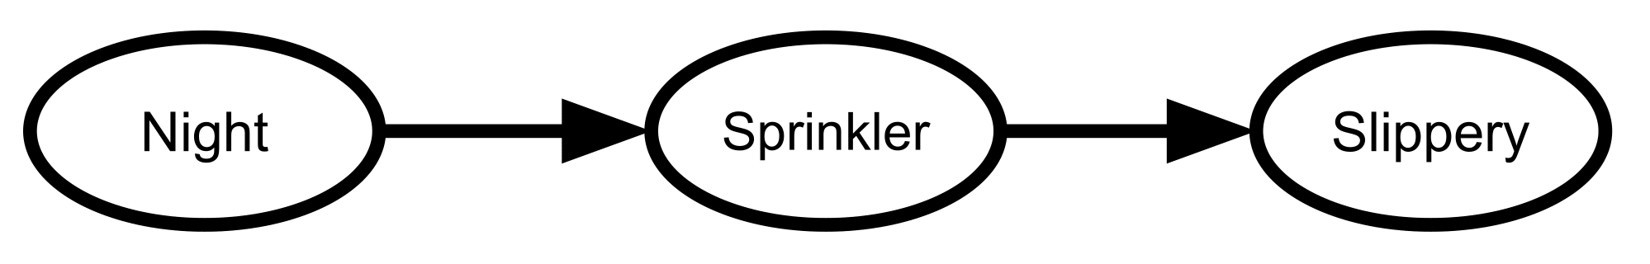
\includegraphics[scale=0.25]{Rationality20From20AI20to20Zombies2020Eliezer20Yudkowsky-img82.jpg}
 }

{
\ \ \ ~}

{
\ \ \ Whether or not it's Night \textit{causes} the
Sprinkler to be on or off, and whether the Sprinkler is on
\textit{causes} the sidewalk to be Slippery or unSlippery.}

{
\ \ \ The direction of the arrows is meaningful. Say we had:}

{
\ \ \ ~}

{
\ \ \  
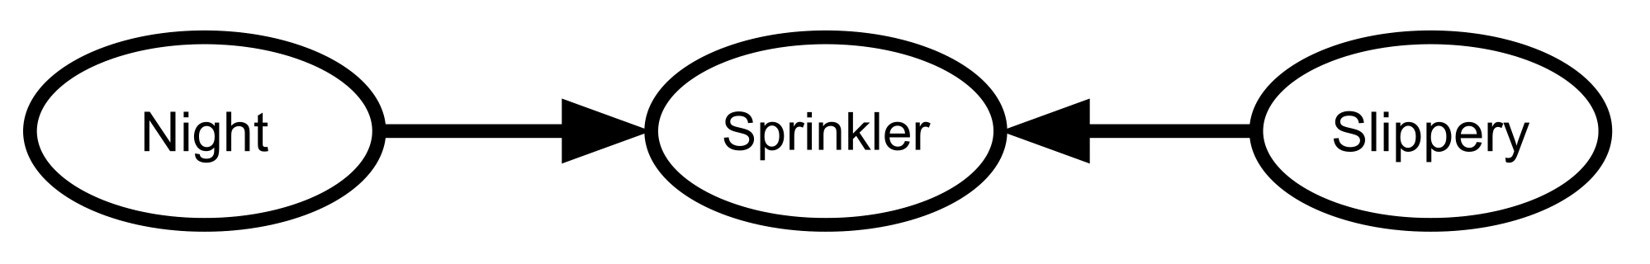
\includegraphics[scale=0.25]{Rationality20From20AI20to20Zombies2020Eliezer20Yudkowsky-img83.jpg}
 }

{
\ \ \ ~}

{
\ \ \ This would mean that, if I \textit{didn't} know
anything about the sprinkler, the probability of Nighttime and
Slipperiness would be independent of each other. For example, suppose
that I roll Die One and Die Two, and add up the showing numbers to get
the Sum:}

{
\ \ \ ~}

{
\ \ \  
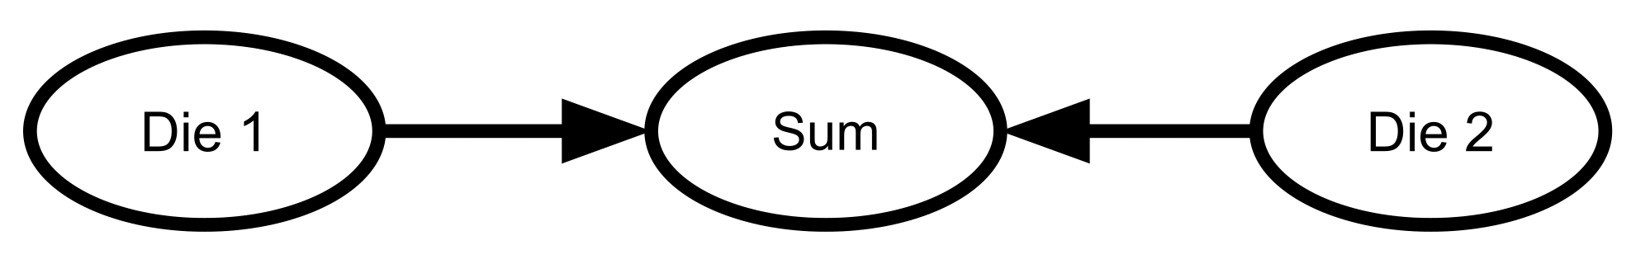
\includegraphics[scale=0.25]{Rationality20From20AI20to20Zombies2020Eliezer20Yudkowsky-img84.jpg}
 }

{
\ \ \ ~}

{
\ \ \ If you don't tell me the sum of the two numbers,
and you tell me the first die showed 6, this doesn't
tell me anything about the result of the second die, yet. But if you
now also tell me the sum is 7, I know the second die showed 1.}

{
\ \ \ Figuring out when various pieces of information are dependent or
independent of each other, given various background knowledge, actually
turns into a quite technical topic. The books to read are Judea
Pearl's \textit{Probabilistic Reasoning in Intelligent
Systems: Networks of Plausible Inference}\textsuperscript{1} and
\textit{Causality: Models, Reasoning, and
Inference}.\textsuperscript{2} (If you only have time to read one book,
read the first one.)}

{
\ \ \ If you know how to read causal graphs, then you look at the
dice-roll graph and immediately see:}

{\centering
\ \ \ P(Die 1, Die 2) = P(Die 1) {\texttimes} P(Die 2)
\par}


\bigskip

{\centering
\ \ \ P(Die 1, Die 2{\textbar}Sum) ${\neq}$ P(Die 1{\textbar}Sum)
{\texttimes} P(Die 2{\textbar}Sum)
\par}


\bigskip

{
\ \ \ If you look at the correct sidewalk diagram, you see facts like:}

{\centering
\ \ \ P(Slippery{\textbar}Night) ${\neq}$ P(Slippery)
\par}


\bigskip

{\centering
\ \ \ P(Slippery{\textbar}Sprinkler) ${\neq}$ P(Slippery)
\par}


\bigskip

{\centering
\ \ \ P(Slippery{\textbar}Night, Sprinkler) =
P(Slippery{\textbar}Sprinkler).
\par}


\bigskip

{
\ \ \ That is, the probability of the sidewalk being Slippery, given
knowledge about the Sprinkler and the Night, is the same probability we
would assign if we knew only about the Sprinkler. Knowledge of the
Sprinkler has made knowledge of the Night irrelevant to inferences
about Slipperiness.}

{
\ \ \ This is known as \textit{screening off}, and the criterion that
lets us read such conditional independences off causal graphs is known
as \textit{D-separation}.}

{
\ \ \ For the case of argument and authority, the causal diagram looks
like this:}

{
\ \ \ ~}

{
\ \ \  
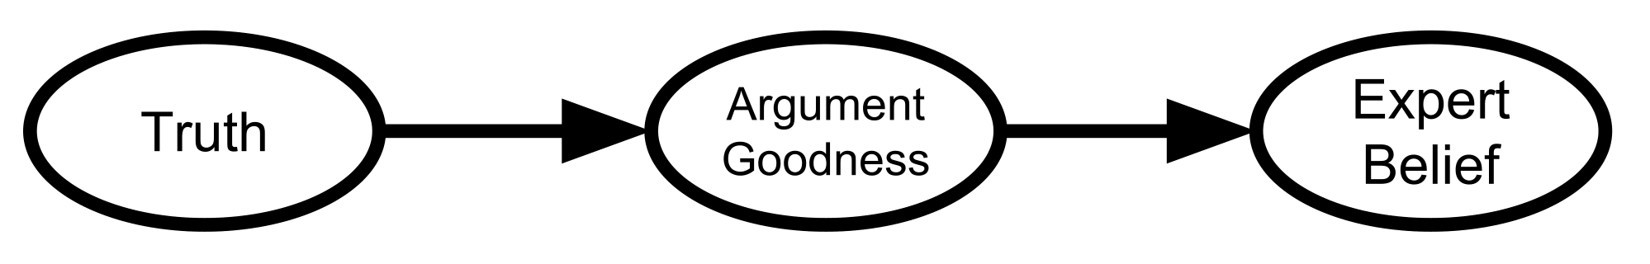
\includegraphics[scale=0.25]{Rationality20From20AI20to20Zombies2020Eliezer20Yudkowsky-img85.jpg}
 }

{
\ \ \ ~}

{
\ \ \ If something is true, then it therefore tends to have arguments in
favor of it, and the experts therefore observe these evidences and
change their opinions. (In theory!)}

{
\ \ \ If we see that an expert believes something, we infer back to the
existence of evidence-in-the-abstract (even though we
don't know what that evidence is exactly), and from the
existence of this abstract evidence, we infer back to the truth of the
proposition.}

{
\ \ \ But if we know the value of the Argument node, this D-separates
the node ``Truth'' from the node
``Expert Belief'' by blocking all
paths between them, according to certain technical criteria for
``path blocking'' that seem pretty
obvious in this case. So even without checking the exact probability
distribution, we can read off from the graph that:}

{\centering
\ \ \ P(truth{\textbar}argument, expert) = P(truth{\textbar}argument).
\par}


\bigskip

{
\ \ \ This does not represent a contradiction of ordinary probability
theory. It's just a more compact way of expressing
certain probabilistic facts. You could read the same equalities and
inequalities off an unadorned probability distribution---but it would
be harder to see it by eyeballing. Authority and argument
don't need two different kinds of probability, any more
than sprinklers are made out of ontologically different stuff than
sunlight. }

{
\ \ \ In practice you can never \textit{completely} eliminate reliance
on authority. Good authorities are more likely to know about any
counterevidence that exists and should be taken into account; a lesser
authority is less likely to know this, which makes their arguments less
reliable. This is not a factor you can eliminate merely by hearing the
evidence they \textit{did} take into account.}

{
\ \ \ It's also very hard to reduce arguments to
\textit{pure} math; and otherwise, judging the strength of an
inferential step may rely on intuitions you can't
duplicate without the same thirty years of experience.}

{
\ \ \ There is an ineradicable legitimacy to assigning \textit{slightly}
higher probability to what E. T. Jaynes tells you about Bayesian
probability, than you assign to Eliezer Yudkowsky making the exact same
statement. Fifty additional years of experience should not count for
literally \textit{zero} influence.}

{
\ \ \ But this slight strength of authority is only \textit{ceteris
paribus}, and can easily be overwhelmed by stronger arguments. I have a
minor erratum in one of Jaynes's books---because
algebra trumps authority.}

{\centering
\ \ \ \ ~
\par}

{\centering
\ \ \ *
\par}


\bigskip

{
\ \ \ 1. Pearl, \textit{Probabilistic Reasoning in Intelligent
Systems}.}

{
\ \ \ 2. Judea Pearl, \textit{Causality: Models, Reasoning, and
Inference}, 2nd ed. (New York: Cambridge University Press, 2009).}

\mysection{Hug the Query}

{
\ \ \ In the art of rationality there is a discipline of
\textit{closeness-to-the-issue}{}---trying to observe evidence that is
as near to the original question as possible, so that it screens off as
many other arguments as possible. }

{
\ \ \ The Wright Brothers say, ``My plane will
fly.'' If you look at their authority (bicycle
mechanics who happen to be excellent amateur physicists) then you will
compare their authority to, say, Lord Kelvin, and you will find that
Lord Kelvin is the greater authority.}

{
\ \ \ If you demand to see the Wright Brothers'
calculations, and you can follow them, and you demand to see Lord
Kelvin's calculations (he probably
doesn't have any apart from his own incredulity), then
authority becomes much less relevant.}

{
\ \ \ If you actually \textit{watch the plane fly}, the calculations
themselves become moot for many purposes, and Kelvin's
authority not even worth considering.}

{
\ \ \ The more \textit{directly} your arguments bear on a question,
without intermediate inferences---the closer the observed nodes are to
the queried node, in the Great Web of Causality---the more powerful the
evidence. It's a theorem of these causal graphs that
you can never get \textit{more} information from distant nodes, than
from strictly closer nodes that screen off the distant ones.}

{
\ \ \ Jerry Cleaver said: ``What does you in is not
failure to apply some high-level, intricate, complicated technique.
It's overlooking the basics. Not keeping your eye on
the ball.''\textsuperscript{1}}

{
\ \ \ Just as it is superior to argue physics than credentials, it is
also superior to argue physics than rationality. Who was more rational,
the Wright Brothers or Lord Kelvin? If we can check their calculations,
we don't have to care! The virtue of a rationalist
cannot \textit{directly} cause a plane to fly.}

{
\ \ \ If you forget this principle, learning about more biases will hurt
you, because it will distract you from more direct arguments.
It's all too easy to argue that someone is exhibiting
Bias \#182 in your repertoire of fully generic accusations, but you
can't \textit{settle} a factual issue without closer
evidence. If there are biased reasons to say the Sun is shining, that
doesn't make it dark out.}

{
\ \ \ Just as you can't always experiment today, you
can't always check the calculations today. Sometimes
you don't know enough background material, sometimes
there's private information, sometimes there just
isn't time. There's a sadly large
number of times when it's worthwhile to judge the
speaker's rationality. You should always do it with a
hollow feeling in your heart, though, a sense that
something's missing.}

{
\ \ \ Whenever you can, dance as near to the original question as
possible---press yourself up against it---get close enough to
\textit{hug the query!}}

{\centering
\ \ \ \ ~
\par}

{\centering
\ \ \ *
\par}


\bigskip

{
\ \ \ 1. Jerry Cleaver, \textit{Immediate Fiction: A Complete Writing
Course} (Macmillan, 2004).}

\mysection{Rationality and the English Language}

{
\ \ \ Responding to my discussion of applause lights, someone said that
my writing reminded them of George Orwell's Politics
and the English Language.\textsuperscript{1} I was honored. Especially
since I'd already thought of today's
topic. }

{
\ \ \ If you \textit{really} want an artist's
perspective on rationality, then read Orwell; he is mandatory reading
for rationalists as well as authors. Orwell was not a scientist, but a
writer; his tools were not numbers, but words; his adversary was not
Nature, but human evil. If you wish to imprison people for years
without trial, you must think of some other way to say it than
``I'm going to imprison Mr. Jennings
for years without trial.'' You must muddy the
listener's thinking, prevent clear images from
outraging conscience. You say, ``Unreliable elements
were subjected to an alternative justice process.''}

{
\ \ \ Orwell was the outraged opponent of totalitarianism and the muddy
thinking in which evil cloaks itself---which is how
Orwell's writings on language ended up as classic
rationalist documents on a level with Feynman, Sagan, or Dawkins.}

{
\ \ \ ``Writers are told to avoid usage of the passive
voice.'' A rationalist whose background comes
\textit{exclusively} from science may fail to see the flaw in the
previous sentence; but anyone who's done a little
writing should see it right away. I wrote the sentence in the passive
voice, without telling you \textit{who} tells authors to avoid passive
voice. Passive voice removes the actor, leaving only the acted-upon.
``Unreliable elements were subjected to an alternative
justice process''---subjected by \textit{whom}? What
does an ``alternative justice
process'' \textit{do}? With enough static noun
phrases, you can keep anything unpleasant from actually
\textit{happening}.}

{
\ \ \ Journal articles are often written in passive voice. (Pardon me,
\textit{some scientists} write their journal articles in passive voice.
It's not as if the articles are being written by no
one, with no one to blame.) It sounds more authoritative to say
``The subjects were administered
Progenitorivox'' than ``I gave each
college student a bottle of 20 Progenitorivox, and told them to take
one every night until they were gone.'' If you remove
the scientist from the description, that leaves only the all-important
data. But in reality the scientist \textit{is} there, and the subjects
\textit{are} college students, and the Progenitorivox
wasn't
``administered'' but handed over
with instructions. Passive voice obscures reality.}

{
\ \ \ Judging from the comments I get, someone will protest that using
the passive voice in a journal article is hardly a sin---after all, if
you \textit{think} about it, you can realize the scientist is there. It
doesn't seem like a logical flaw. And this is why
rationalists need to read Orwell, not just Feynman or even Jaynes.}

{
\ \ \ Nonfiction conveys \textit{knowledge}, fiction conveys
\textit{experience.} Medical science can extrapolate what would happen
to a human unprotected in a vacuum. Fiction can make you live through
it.}

{
\ \ \ Some rationalists will try to analyze a misleading phrase, try to
see if there \textit{might possibly} be anything meaningful to it, try
to \textit{construct} a logical interpretation. They will be
charitable, give the author the benefit of the doubt. Authors, on the
other hand, are trained \textit{not} to give themselves the benefit of
the doubt. Whatever the audience \textit{thinks} you said \textit{is}
what you said, whether you meant to say it or not; you
can't argue with the audience no matter how clever your
justifications.}

{
\ \ \ A writer knows that readers will \textit{not} stop for a minute to
think. A fictional experience is a continuous stream of first
impressions. A writer-rationalist pays attention to the
\textit{experience} words create. If you are evaluating the public
rationality of a statement, and you analyze the words deliberatively,
rephrasing propositions, trying out different meanings, searching for
nuggets of truthiness, then you're losing track of the
first impression---what the audience \textit{sees}, or rather
\textit{feels.}}

{
\ \ \ A novelist would notice the screaming wrongness of
``The subjects were administered
Progenitorivox.'' What life is here for a reader to
live? This sentence creates a distant feeling of authoritativeness, and
that's \textit{all}{}---the \textit{only} experience is
the feeling of being told something reliable. A novelist would see
nouns too abstract to show what actually happened---the postdoc with
the bottle in their hand, trying to look stern; the student listening
with a nervous grin.}

{
\ \ \ My point is not to say that journal articles should be written
like novels, but that a rationalist should become consciously aware of
the \textit{experiences} which words create. A rationalist must
understand the mind and how to operate it. That includes the stream of
consciousness, the part of yourself that unfolds in language. A
rationalist must become consciously aware of the actual, experiential
impact of phrases, beyond their mere propositional semantics.}

{
\ \ \ Or to say it more bluntly: \textit{Meaning does not excuse
impact!}}

{
\ \ \ I don't care what rational interpretation you can
\textit{construct} for an applause light like ``AI
should be developed through democratic processes.''
That cannot excuse its irrational impact of signaling the audience to
applaud, not to mention its cloudy question-begging vagueness.}

{
\ \ \ Here is Orwell, railing against the \textit{impact} of cliches,
their effect on the experience of thinking:}

{
\ \ \ When one watches some tired hack on the platform mechanically
repeating the familiar phrases---BESTIAL, ATROCITIES, IRON HEEL,
BLOODSTAINED TYRANNY, FREE PEOPLES OF THE WORLD, STAND SHOULDER TO
SHOULDER---one often has a curious feeling that one is not watching a
live human being but some kind of dummy .~.~. A speaker who uses that
kind of phraseology has gone some distance toward turning himself into
a machine. The appropriate noises are coming out of his larynx, but his
brain is not involved, as it would be if he were choosing his words for
himself .~.~.}

{
\ \ \ What is above all needed is to let the meaning choose the word,
and not the other way around. In prose, the worst thing one can do with
words is surrender to them. When you think of a concrete object, you
think wordlessly, and then, if you want to describe the thing you have
been visualising you probably hunt about until you find the exact words
that seem to fit it. When you think of something abstract you are more
inclined to use words from the start, and unless you make a conscious
effort to prevent it, the existing dialect will come rushing in and do
the job for you, at the expense of blurring or even changing your
meaning. Probably it is better to put off using words as long as
possible and get one's meaning as clear as one can
through pictures and sensations.}

{
\ \ \ Charles Sanders Peirce might have written that last paragraph.
More than one path can lead to the Way.}

{\centering
\ \ \ \ ~
\par}

{\centering
\ \ \ *
\par}


\bigskip

{
\ \ \ 1. George Orwell, ``Politics and the English
Language,'' \textit{Horizon} (April 1946).}

\mysection{Human Evil and Muddled Thinking}

{
\ \ \ George Orwell saw the descent of the civilized world into
totalitarianism, the conversion or corruption of one country after
another; the boot stamping on a human face, forever, and remember that
it is forever. You were born too late to remember a time when the rise
of totalitarianism seemed unstoppable, when one country after another
fell to secret police and the thunderous knock at midnight, while the
professors of free universities hailed the Soviet
Union's purges as progress. It feels as alien to you as
fiction; it is hard for you to take seriously. Because, in your branch
of time, the Berlin Wall fell. And if Orwell's name is
not carved into one of those stones, it should be. }

{
\ \ \ Orwell saw the destiny of the human species, and he put forth a
convulsive effort to wrench it off its path. Orwell's
weapon was clear writing. Orwell knew that muddled language is muddled
thinking; he knew that human evil and muddled thinking intertwine like
conjugate strands of DNA:\textsuperscript{1}}

{
\ \ \ In our time, political speech and writing are largely the defence
of the indefensible. Things like the continuance of British rule in
India, the Russian purges and deportations, the dropping of the atom
bombs on Japan, can indeed be defended, but only by arguments which are
too brutal for most people to face, and which do not square with the
professed aims of the political parties. Thus political language has to
consist largely of euphemism, question-begging and sheer cloudy
vagueness. Defenceless villages are bombarded from the air, the
inhabitants driven out into the countryside, the cattle machine-gunned,
the huts set on fire with incendiary bullets: this is called
PACIFICATION .~.~.}

{
\ \ \ Orwell was clear on the goal of his clarity:}

{
\ \ \ If you simplify your English, you are freed from the worst follies
of orthodoxy. You cannot speak any of the necessary dialects, and when
you make a stupid remark its stupidity will be obvious, even to
yourself.}

{
\ \ \ To make our stupidity obvious, even to ourselves---this is the
heart of \textit{Overcoming Bias}.}

{
\ \ \ Evil sneaks, hidden, through the unlit shadows of the mind. We
look back with the clarity of history, and weep to remember the planned
famines of Stalin and Mao, which killed tens of millions. We call this
evil, because it was done by deliberate human intent to inflict pain
and death upon innocent human beings. We call this evil, because of the
revulsion that we feel against it, looking back with the clarity of
history. For perpetrators of evil to avoid its natural opposition, the
revulsion must remain latent. Clarity must be avoided at any cost. Even
as humans of clear sight tend to oppose the evil that they see; so too
does human evil, wherever it exists, set out to muddle thinking.}

{
\ \ \ \textit{1984} sets this forth starkly: Orwell's
ultimate villains are cutters and airbrushers of photographs (based on
historical cutting and airbrushing in the Soviet Union). At the peak of
all darkness in the Ministry of Love, O'Brien tortures
Winston to admit that two plus two equals five:\textsuperscript{2}}

{
\ \ \ ``Do you remember,'' he went
on, ``writing in your diary, `Freedom
is the freedom to say that two plus two make
four'?''}

{
\ \ \ ``Yes,'' said Winston.}

{
\ \ \ O'Brien held up his left hand, its back towards
Winston, with the thumb hidden and the four fingers extended.}

{
\ \ \ ``How many fingers am I holding up,
Winston?''}

{
\ \ \ ``Four.''}

{
\ \ \ ``And if the party says that it is not four but
five---then how many?''}

{
\ \ \ ``Four.''}

{
\ \ \ The word ended in a gasp of pain. The needle of the dial had shot
up to fifty-five. The sweat had sprung out all over
Winston's body. The air tore into his lungs and issued
again in deep groans which even by clenching his teeth he could not
stop. O'Brien watched him, the four fingers still
extended. He drew back the lever. This time the pain was only slightly
eased.}

{
\ \ \ I am continually aghast at apparently intelligent folks---such as
Robin Hanson's colleague Tyler Cowen{}---who
don't think that overcoming bias is important. This is
your \textit{mind} we're talking about. Your human
intelligence. It separates you from an ape. It built this world. You
don't think how the mind works is important? You
don't think the mind's systematic
malfunctions are important? Do you think the Inquisition would have
tortured witches, if all were ideal Bayesians?}

{
\ \ \ Tyler Cowen apparently feels that overcoming bias is just as
biased as bias: ``I view Robin's blog
as exemplifying bias, and indeed showing that bias can be very
useful.'' I \textit{hope} this is only the result of
thinking too abstractly while trying to sound clever. Does Tyler
seriously think that scope insensitivity to the value of human life is
on the same level with trying to create plans that will \textit{really}
save as many lives as possible?}

{
\ \ \ Orwell was forced to fight a similar attitude---that to admit to
any distinction is youthful naiveté:}

{
\ \ \ Stuart Chase and others have come near to claiming that all
abstract words are meaningless, and have used this as a pretext for
advocating a kind of political quietism. Since you
don't know what Fascism is, how can you struggle
against Fascism?}

{
\ \ \ Maybe overcoming bias doesn't look quite exciting
enough, if it's framed as a struggle against mere
accidental mistakes. Maybe it's harder to get excited
if there isn't some clear evil to oppose. So let us be
absolutely clear that where there is human evil in the world, where
there is cruelty and torture and deliberate murder, there are biases
enshrouding it. Where people of clear sight oppose these biases, the
concealed evil fights back. The truth \textit{does} have enemies. If
\textit{Overcoming Bias} were a newsletter in the old Soviet Union,
every poster and commenter of \textit{Overcoming Bias} would have been
shipped off to labor camps.}

{
\ \ \ In all human history, every great leap forward has been driven by
a new clarity of thought. Except for a few natural catastrophes, every
great woe has been driven by a stupidity. Our last enemy is ourselves;
and this is a war, and we are soldiers.}

{\centering
\ \ \ \ ~
\par}

{\centering
\ \ \ *
\par}


\bigskip

{
\ \ \ 1. Ibid.}

{
\ \ \ 2. George Orwell, \textit{1984} (Signet Classic, 1950).}


\chapter{Against Rationalization}

\mysection{Knowing About Biases Can Hurt People}

{
\ \ \ Once upon a time I tried to tell my mother about the problem of
expert calibration, saying: ``So when an expert says
they're 99\% confident, it only happens about 70\% of
the time.'' Then there was a pause as, suddenly, I
realized I was talking to my mother, and I hastily added:
``Of course, you've got to make sure
to apply that skepticism evenhandedly, including to yourself, rather
than just using it to argue against anything you disagree
with---'' }

{
\ \ \ And my mother said: ``Are you kidding? This is
great! I'm going to use it all the
time!''}

{
\ \ \ Taber and Lodge's ``Motivated
skepticism in the evaluation of political beliefs''
describes the confirmation of six predictions:\textsuperscript{1}}

{
\ \ \ Prior attitude effect. Subjects who feel strongly about an
issue---even when encouraged to be objective---will evaluate supportive
arguments more favorably than contrary arguments.}

{
\ \ \ Disconfirmation bias. Subjects will spend more time and cognitive
resources denigrating contrary arguments than supportive arguments.}

{
\ \ \ Confirmation bias. Subjects free to choose their information
sources will seek out supportive rather than contrary sources.}

{
\ \ \ \textbf{Attitude polarization. Exposing subjects to an apparently
balanced set of pro and con arguments will exaggerate their initial
polarization.}}

{
\ \ \ Attitude strength effect. Subjects voicing stronger attitudes will
be more prone to the above biases.}

{
\ \ \ \textbf{Sophistication effect. Politically knowledgeable subjects,
because they possess greater ammunition with which to counter-argue
incongruent facts and arguments, will be more prone to the above
biases.}}

{
\ \ \ If you're irrational to start with, having
\textit{more} knowledge can \textit{hurt} you. For a true Bayesian,
information would never have negative expected utility. But humans
aren't perfect Bayes-wielders; if we're
not careful, we can cut ourselves.}

{
\ \ \ I've \textit{seen} people severely messed up by
their own knowledge of biases. They have more ammunition with which to
argue against anything they don't like. And that
problem---too much ready ammunition---is one of the primary ways that
people with high mental agility end up stupid, in
Stanovich's
``dysrationalia'' sense of
stupidity.}

{
\ \ \ You can think of people who fit this description, right? People
with high g-factor who end up being \textit{less} effective because
they are too sophisticated as arguers? Do you think
you'd be helping them---making them more effective
rationalists---if you just told them about a list of classic biases?}

{
\ \ \ I recall someone who learned about the calibration/overconfidence
problem. Soon after he said: ``Well, you
can't trust experts; they're wrong so
often---as experiments have shown. So therefore, when I predict the
future, I prefer to assume that things will continue historically as
they have---'' and went off into this whole complex,
error-prone, highly questionable extrapolation. Somehow, when it came
to trusting his own preferred conclusions, all those biases and
fallacies seemed much less \textit{salient}{}---leapt much less readily
to mind---than when he needed to counter-argue someone else.}

{
\ \ \ I told the one about the problem of disconfirmation bias and
sophisticated argument, and lo and behold, the next time I said
something he didn't like, he accused me of being a
sophisticated arguer. He didn't try to point out any
particular sophisticated argument, any particular flaw---just shook his
head and sighed sadly over how I was apparently using my own
intelligence to defeat itself. He had acquired yet another Fully
General Counterargument.}

{
\ \ \ Even the notion of a ``sophisticated
arguer'' can be deadly, if it leaps all too readily
to mind when you encounter a seemingly intelligent person who says
something you don't like.}

{
\ \ \ I endeavor to learn from my mistakes. The last time I gave a talk
on heuristics and biases, I started out by introducing the general
concept by way of the conjunction fallacy and representativeness
heuristic. And then I moved on to confirmation bias, disconfirmation
bias, sophisticated argument, motivated skepticism, and other attitude
effects. I spent the next thirty minutes \textit{hammering} on that
theme, reintroducing it from as many different perspectives as I
could.}

{
\ \ \ I wanted to get my audience interested in the subject. Well, a
simple description of conjunction fallacy and representativeness would
suffice for that. But suppose they did get interested. Then what? The
literature on bias is mostly cognitive psychology for cognitive
psychology's sake. I had to give my audience their dire
warnings during that one lecture, or they probably
wouldn't hear them at all.}

{
\ \ \ Whether I do it on paper, or in speech, I now try to never mention
calibration and overconfidence unless I have first talked about
disconfirmation bias, motivated skepticism, sophisticated arguers, and
dysrationalia in the mentally agile. First, do no harm!}

{\centering
\ \ \ \ ~
\par}

{\centering
\ \ \ *
\par}


\bigskip

{
\ \ \ 1. Charles S. Taber and Milton Lodge, ``Motivated
Skepticism in the Evaluation of Political Beliefs,''
\textit{American Journal of Political Science} 50, no. 3 (2006):
755--769, doi:10.1111/j.1540-5907.2006.00214.x.}

\mysection{Update Yourself Incrementally}

{
\ \ \ Politics is the mind-killer. Debate is war, arguments are
soldiers. There is the temptation to search for ways to interpret every
possible experimental result to confirm your theory, like securing a
citadel against every possible line of attack. This you cannot do. It
is mathematically impossible. For every expectation of evidence, there
is an equal and opposite expectation of counterevidence. }

{
\ \ \ But it's okay if your cherished belief
isn't \textit{perfectly} defended. If the hypothesis is
that the coin comes up heads 95\% of the time, then one time in twenty
you will expect to see what looks like contrary evidence. This is okay.
It's normal. It's even expected, so
long as you've got nineteen supporting observations for
every contrary one. A probabilistic model can take a hit or two, and
still survive, so long as the hits don't \textit{keep
on} coming in.}

{
\ \ \ Yet it is widely believed, especially in the court of public
opinion, that a true theory can have \textit{no} failures and a false
theory \textit{no} successes.}

{
\ \ \ You find people holding up a single piece of what they conceive to
be evidence, and claiming that their theory can
``explain'' it, as though this were
all the support that any theory needed. Apparently a false theory can
have \textit{no} supporting evidence; it is impossible for a false
theory to fit even a single event. Thus, a single piece of confirming
evidence is all that any theory needs.}

{
\ \ \ It is only slightly less foolish to hold up a single piece of
\textit{probabilistic} counterevidence as disproof, as though it were
impossible for a correct theory to have even a \textit{slight} argument
against it. But this is how humans have argued for ages and ages,
trying to defeat all enemy arguments, while denying the enemy even a
single shred of support. People want their debates to be one-sided;
they are accustomed to a world in which their preferred theories have
not one iota of antisupport. Thus, allowing a single item of
probabilistic counterevidence would be the end of the world.}

{
\ \ \ I just know someone in the audience out there is going to say,
``But you \textit{can't} concede even
a single point if you want to win debates in the real world! If you
concede that any counterarguments exist, the Enemy will harp on them
over and over---you can't let the Enemy do that!
You'll \textit{lose!} What could be more viscerally
terrifying than \textit{that?}''}

{
\ \ \ Whatever. Rationality is not for winning debates, it is for
deciding which side to join. If you've already decided
which side to argue for, the work of rationality is \textit{done}
within you, whether well or poorly. But how can you, yourself, decide
which side to argue? If \textit{choosing the wrong side} is viscerally
terrifying, even just a little viscerally terrifying,
you'd best integrate \textit{all} the evidence.}

{
\ \ \ Rationality is not a walk, but a dance. On each step in that dance
your foot should come down in exactly the correct spot, neither to the
left nor to the right. Shifting belief upward with each iota of
confirming evidence. Shifting belief downward with each iota of
contrary evidence. Yes, \textit{down.} Even with a correct model, if it
is not an exact model, you will sometimes need to revise your belief
\textit{down.}}

{
\ \ \ If an iota or two of evidence happens to countersupport your
belief, that's okay. It happens, sometimes, with
probabilistic evidence for non-exact theories. (If an exact theory
fails, you \textit{are} in trouble!) Just shift your belief downward a
little---the probability, the odds ratio, or even a nonverbal weight of
credence in your mind. Just shift downward a little, and wait for more
evidence. If the theory is true, supporting evidence will come in
shortly, and the probability will climb again. If the theory is false,
you don't really want it anyway.}

{
\ \ \ The problem with using black-and-white, binary, qualitative
reasoning is that any single observation either destroys the theory or
it does not. When not even a single contrary observation is allowed, it
creates cognitive dissonance and has to be argued away. And this rules
out incremental progress; it rules out correct integration of all the
evidence. Reasoning probabilistically, we realize that on average, a
correct theory will generate a greater weight of support than
countersupport. And so you can, \textit{without fear,} say to yourself:
``This is gently contrary evidence, I will shift my
belief downward.'' Yes, \textit{down.} It does not
destroy your cherished theory. That is qualitative reasoning; think
quantitatively.}

{
\ \ \ For every expectation of evidence, there is an equal and opposite
expectation of counterevidence. On every occasion, you must, on
average, anticipate revising your beliefs downward as much as you
anticipate revising them upward. If you think you already know what
evidence will come in, then you must already be fairly sure of your
theory---probability close to 1---which doesn't leave
much room for the probability to go further upward. And however
unlikely it seems that you will encounter disconfirming evidence, the
resulting downward shift must be large enough to precisely balance the
anticipated gain on the other side. The weighted mean of your expected
posterior probability must equal your prior probability.}

{
\ \ \ How silly is it, then, to be terrified of revising your
probability downward, if you're bothering to
investigate a matter at all? On average, you must anticipate as much
downward shift as upward shift from every individual observation.}

{
\ \ \ It may perhaps happen that an iota of antisupport comes in again,
and again and again, while new support is slow to trickle in. You may
find your belief drifting downward and further downward. Until,
finally, you realize from which quarter the winds of evidence are
blowing against you. In that moment of realization, there is no point
in constructing excuses. In that moment of realization, you have
\textit{already relinquished} your cherished belief. Yay! Time to
celebrate! Pop a champagne bottle or send out for pizza! You
can't become stronger by keeping the beliefs you
started with, after all.}

{\centering
\ \ \ \ ~
\par}

{\centering
\ \ \ *
\par}

\mysection{One Argument Against An Army}

{
\ \ \ I talked about a style of reasoning in which not a single contrary
argument is allowed, with the result that every non-supporting
observation has to be argued away. Here I suggest that when people
encounter a contrary argument, they prevent themselves from
downshifting their confidence by \textit{rehearsing} already-known
support. }

{
\ \ \ Suppose the country of Freedonia is debating whether its neighbor,
Sylvania, is responsible for a recent rash of meteor strikes on its
cities. There are several pieces of evidence suggesting this: the
meteors struck cities close to the Sylvanian border; there was unusual
activity in the Sylvanian stock markets \textit{before} the strikes;
and the Sylvanian ambassador Trentino was heard muttering about
``heavenly vengeance.''}

{
\ \ \ Someone comes to you and says: ``I
don't think Sylvania is responsible for the meteor
strikes. They have trade with us of billions of dinars
annually.''
``Well,'' you reply,
``the meteors struck cities close to Sylvania, there
was suspicious activity in their stock market, and their ambassador
spoke of heavenly vengeance afterward.'' Since these
three arguments outweigh the first, you \textit{keep} your belief that
Sylvania is responsible---you believe rather than disbelieve,
qualitatively. Clearly, the balance of evidence weighs against
Sylvania.}

{
\ \ \ Then another comes to you and says: ``I
don't think Sylvania is responsible for the meteor
strikes. Directing an asteroid strike is really hard. Sylvania
doesn't even have a space program.''
You reply, ``But the meteors struck cities close to
Sylvania, and their investors knew it, and the ambassador came right
out and admitted it!'' Again, these three arguments
outweigh the first (by three arguments against one argument), so you
keep your belief that Sylvania is responsible.}

{
\ \ \ Indeed, your convictions are \textit{strengthened.} On two
separate occasions now, you have evaluated the balance of evidence, and
both times the balance was tilted against Sylvania by a ratio of 3 to
1.}

{
\ \ \ You encounter further arguments by the pro-Sylvania
traitors---again, and again, and a hundred times again---but each time
the new argument is handily defeated by 3 to 1. And on every occasion,
you feel yourself becoming more confident that Sylvania was indeed
responsible, shifting your prior according to the felt balance of
evidence.}

{
\ \ \ The problem, of course, is that by \textit{rehearsing} arguments
you \textit{already knew}, you are double-counting the evidence. This
would be a grave sin even if you double-counted \textit{all} the
evidence. (Imagine a scientist who does an experiment with 50 subjects
and fails to obtain statistically significant results, so the scientist
counts all the data twice.)}

{
\ \ \ But to selectively double-count \textit{only some} evidence is
sheer farce. I remember seeing a cartoon as a child, where a villain
was dividing up loot using the following algorithm:
``One for you, one for me. One for you, one-two for
me. One for you, one-two-three for me.''}

{
\ \ \ As I emphasized in the last essay, even if a cherished belief is
\textit{true}, a rationalist may sometimes need to downshift the
probability while integrating \textit{all} the evidence. Yes, the
balance of support may still favor your cherished belief. But you still
have to shift the probability \textit{down}{}---yes,
\textit{down}{}---from whatever it was before you heard the contrary
evidence. It does no good to \textit{rehearse} supporting arguments,
because you have already taken those into account.}

{
\ \ \ And yet it does appear to me that when people are confronted by a
\textit{new} counterargument, they search for a justification not to
downshift their confidence, and of course they find supporting
arguments they \textit{already know.} I have to keep constant vigilance
not to do this myself! It feels as natural as parrying a sword-strike
with a handy shield.}

{
\ \ \ With the right kind of wrong reasoning, a handful of support---or
even a single argument---can stand off an army of contradictions.}

{\centering
\ \ \ \ ~
\par}

{\centering
\ \ \ *
\par}

\mysection{The Bottom Line}

{
\ \ \ There are two sealed boxes up for auction, box A and box B. One
and only one of these boxes contains a valuable diamond. There are all
manner of signs and portents indicating whether a box contains a
diamond; but I have no sign which I \textit{know} to be perfectly
reliable. There is a blue stamp on one box, for example, and I know
that boxes which contain diamonds are more likely than empty boxes to
show a blue stamp. Or one box has a shiny surface, and I have a
suspicion---I am not sure---that no diamond-containing box is ever
shiny. }

{
\ \ \ Now suppose there is a clever arguer, holding a sheet of paper,
and they say to the owners of box A and box B: ``Bid
for my services, and whoever wins my services, I shall argue that their
box contains the diamond, so that the box will receive a higher
price.'' So the box-owners bid, and box
B's owner bids higher, winning the services of the
clever arguer.}

{
\ \ \ The clever arguer begins to organize their thoughts. First, they
write, ``And \textit{therefore}, box B contains the
diamond!'' at the bottom of their sheet of paper.
Then, at the top of the paper, the clever arguer writes,
``Box B shows a blue stamp,'' and
beneath it, ``Box A is shiny,'' and
then, ``Box B is lighter than box
A,'' and so on through many signs and portents; yet
the clever arguer neglects all those signs which might argue in favor
of box A. And then the clever arguer comes to me and recites from their
sheet of paper: ``Box B shows a blue stamp, and box A
is shiny,'' and so on, until they reach:
``and \textit{therefore}, box B contains the
diamond.''}

{
\ \ \ But consider: At the moment when the clever arguer wrote down
their conclusion, at the moment they put ink on their sheet of paper,
the evidential entanglement of that physical ink with the physical
boxes became fixed.}

{
\ \ \ It may help to visualize a collection of worlds---Everett branches
or Tegmark duplicates{}---within which there is some objective
frequency at which box A or box B contains a diamond.
There's likewise some objective frequency within the
subset ``worlds with a shiny box A''
where box B contains the diamond; and some objective frequency in
``worlds with shiny box A and blue-stamped box
B'' where box B contains the diamond.}

{
\ \ \ The ink on paper is formed into odd shapes and curves, which look
like this text: ``And \textit{therefore}, box B
contains the diamond.'' If you happened to be a
literate English speaker, you might become confused, and think that
this shaped ink somehow \textit{meant} that box B contained the
diamond. Subjects instructed to say the color of printed pictures and
shown the picture GREEN often say
``green'' instead of
``red.'' It helps to be illiterate,
so that you are not confused by the shape of the ink.}

{
\ \ \ To us, the true import of a thing is its entanglement with other
things. Consider again the collection of worlds, Everett branches or
Tegmark duplicates. At the moment when all clever arguers in all worlds
put ink to the bottom line of their paper---let us suppose this is a
single moment---it fixed the correlation of the ink with the boxes. The
clever arguer writes in non-erasable pen; the ink will not change. The
boxes will not change. Within the subset of worlds where the ink says
``And therefore, box B contains the
diamond,'' there is already some fixed percentage of
worlds where box A contains the diamond. This will not change
regardless of what is written in on the blank lines above.}

{
\ \ \ So the evidential entanglement of the ink is fixed, and I leave to
you to decide what it might be. Perhaps box owners who believe a better
case can be made for them are more liable to hire advertisers; perhaps
box owners who fear their own deficiencies bid higher. If the box
owners do not themselves understand the signs and portents, then the
ink will be completely unentangled with the boxes'
contents, though it may tell you something about the
owners' finances and bidding habits.}

{
\ \ \ Now suppose another person present is genuinely curious, and they
\textit{first} write down all the distinguishing signs of \textit{both}
boxes on a sheet of paper, and then apply their knowledge and the laws
of probability and write down at the bottom:
``\textit{Therefore,} I estimate an 85\% probability
that box B contains the diamond.'' Of what is this
handwriting evidence? Examining the chain of cause and effect leading
to this physical ink on physical paper, I find that the chain of
causality wends its way through all the signs and portents of the
boxes, and is dependent on these signs; for in worlds with different
portents, a different probability is written at the bottom.}

{
\ \ \ So the handwriting of the curious inquirer is entangled with the
signs and portents and the contents of the boxes, whereas the
handwriting of the clever arguer is evidence only of which owner paid
the higher bid. There is a great difference in the indications of ink,
though one who foolishly read aloud the ink-shapes might think the
English words sounded similar.}

{
\ \ \ Your effectiveness as a rationalist is determined by whichever
algorithm actually writes the bottom line of your thoughts. If your car
makes metallic squealing noises when you brake, and you
aren't willing to face up to the financial cost of
getting your brakes replaced, you can decide to look for reasons why
your car might not need fixing. But the actual percentage of you that
survive in Everett branches or Tegmark worlds---which we will take to
describe your effectiveness as a rationalist---is determined by the
algorithm that decided \textit{which} conclusion you would seek
arguments for. In this case, the real algorithm is
``Never repair anything expensive.''
If this is a good algorithm, fine; if this is a bad algorithm, oh well.
The arguments you write afterward, above the bottom line, will not
change anything either way.}

{
\ \ \ This is intended as a caution for your own thinking, not a Fully
General Counterargument against conclusions you don't
like. For it is indeed a clever argument to say ``My
opponent is a clever arguer,'' if you are paying
yourself to retain whatever beliefs you had at the start. The
world's cleverest arguer may point out that the Sun is
shining, and yet it is still probably daytime.}

{\centering
\ \ \ \ ~
\par}

{\centering
\ \ \ *
\par}

\mysection{What Evidence Filtered Evidence?}

{
\ \ \ I discussed the dilemma of the clever arguer, hired to sell you a
box that may or may not contain a diamond. The clever arguer points out
to you that the box has a blue stamp, and it is a valid known fact that
diamond-containing boxes are more likely than empty boxes to bear a
blue stamp. What happens at this point, from a Bayesian perspective?
Must you helplessly update your probabilities, as the clever arguer
wishes? }

{
\ \ \ If you can look at the box yourself, you can add up all the signs
yourself. What if you can't look? What if the only
evidence you have is the word of the clever arguer, who is legally
constrained to make only true statements, but does not tell you
everything they know? Each statement that the clever arguer makes is
valid evidence---how could you \textit{not} update your probabilities?
Has it ceased to be true that, in such-and-such a proportion of Everett
branches or Tegmark duplicates in which box B has a blue stamp, box B
contains a diamond? According to Jaynes, a Bayesian must always
condition on all known evidence, on pain of paradox. But then the
clever arguer can make you believe anything they choose, if there is a
sufficient variety of signs to selectively report. That
doesn't sound right.}

{
\ \ \ Consider a simpler case, a biased coin, which may be biased to
come up 2/3 heads and 1/3 tails, or 1/3 heads and 2/3 tails, both cases
being equally likely a priori. Each H observed is 1 bit of evidence for
an H-biased coin; each T observed is 1 bit of evidence for a T-biased
coin. I flip the coin ten times, and then I tell you,
``The 4th flip, 6th flip, and 9th flip came up
heads.'' What is your posterior probability that the
coin is H-biased?}

{
\ \ \ And the answer is that it could be almost anything, depending on
what chain of cause and effect lay behind my utterance of those
words---my selection of which flips to report.}

{
\ \ \ I might be following the algorithm of reporting the result of the
4th, 6th, and 9th flips, regardless of the result of those and all
other flips. If you know that I used this algorithm, the posterior odds
are 8:1 in favor of an H-biased coin.}

{
\ \ \ I could be reporting on all flips, and only flips, that came up
heads. In this case, you know that all 7 other flips came up tails, and
the posterior odds are 1:16 against the coin being H-biased.}

{
\ \ \ I could have decided in advance to say the result of the 4th, 6th,
and 9th flips only if the probability of the coin being H-biased
exceeds 98\%. And so on.}

{
\ \ \ Or consider the Monty Hall problem:}

{
\ \ \ On a game show, you are given the choice of three doors leading to
three rooms. You know that in one room is \$100,000, and the other two
are empty. The host asks you to pick a door, and you pick door \#1.
Then the host opens door \#2, revealing an empty room. Do you want to
switch to door \#3, or stick with door \#1?}

{
\ \ \ The answer depends on the host's algorithm. If the
host always opens a door and always picks a door leading to an empty
room, then you should switch to door \#3. If the host always opens door
\#2 regardless of what is behind it, \#1 and \#3 both have 50\%
probabilities of containing the money. If the host only opens a door,
at all, if you initially pick the door with the money, then you should
definitely stick with \#1.}

{
\ \ \ You shouldn't just condition on \#2 being empty,
but this fact plus the fact of the host \textit{choosing} to open door
\#2. Many people are confused by the standard Monty Hall problem
because they update only on \#2 being empty, in which case \#1 and \#3
have equal probabilities of containing the money. This is why Bayesians
are commanded to condition on all of their knowledge, on pain of
paradox.}

{
\ \ \ When someone says, ``The 4th coinflip came up
heads,'' we are not conditioning on the 4th coinflip
having come up heads---we are not taking the subset of all possible
worlds where the 4th coinflip came up heads---rather we are
conditioning on the subset of all possible worlds where a speaker
following some particular algorithm \textit{said}
``The 4th coinflip came up heads.''
The spoken sentence is not the fact itself; don't be
led astray by the mere meanings of words.}

{
\ \ \ Most legal processes work on the theory that every case has
exactly two opposed sides and that it is easier to find two biased
humans than one unbiased one. Between the prosecution and the defense,
\textit{someone} has a motive to present any given piece of evidence,
so the court will see all the evidence; that is the theory. If there
are two clever arguers in the box dilemma, it is not quite as good as
one curious inquirer, but it is almost as good. But that is with two
boxes. Reality often has many-sided problems, and deep problems, and
nonobvious answers, which are not readily found by Blues and Greens
screaming at each other.}

{
\ \ \ Beware lest you abuse the notion of evidence-filtering as a Fully
General Counterargument to exclude all evidence you
don't like: ``That argument was
filtered, therefore I can ignore it.'' If
you're ticked off by a contrary argument, then you are
familiar with the case, and care enough to take sides. You probably
already know your own side's strongest arguments. You
have no reason to infer, from a contrary argument, the existence of new
favorable signs and portents which you have not yet seen. So you are
left with the uncomfortable facts themselves; a blue stamp on box B is
still evidence.}

{
\ \ \ But if you are hearing an argument for the first time, and you are
only hearing one side of the argument, then indeed you should beware!
In a way, no one can \textit{really} trust the theory of natural
selection until after they have listened to creationists for five
minutes; and \textit{then} they know it's solid.}

{\centering
\ \ \ \ ~
\par}

{\centering
\ \ \ *
\par}

\mysection{Rationalization}

{
\ \ \ In The Bottom Line, I presented the dilemma of two boxes, only one
of which contains a diamond, with various signs and portents as
evidence. I dichotomized the curious inquirer and the clever arguer.
The curious inquirer writes down all the signs and portents, and
processes them, and finally writes down
``\textit{Therefore,} I estimate an 85\% probability
that box B contains the diamond.'' The clever arguer
works for the highest bidder, and begins by writing,
``\textit{Therefore,} box B contains the
diamond,'' and then selects favorable signs and
portents to list on the lines above. }

{
\ \ \ The first procedure is rationality. The second procedure is
generally known as
``rationalization.''}

{
\ \ \ ``Rationalization.'' What a
curious term. I would call it a \textit{wrong word.} You cannot
``rationalize'' what is not already
rational. It is as if ``lying'' were
called ``truthization.''}

{
\ \ \ On a purely computational level, there is a rather large
difference between:}

{
\ \ \ Starting from evidence, and then crunching probability flows, in
order to output a probable conclusion. (Writing down all the signs and
portents, and then flowing forward to a probability on the bottom line
which depends on those signs and portents.)}

{
\ \ \ Starting from a conclusion, and then crunching probability flows,
in order to output evidence apparently favoring that conclusion.
(Writing down the bottom line, and then flowing backward to select
signs and portents for presentation on the lines above.)}

{
\ \ \ What fool devised such confusingly similar words,
``rationality'' and
``rationalization,'' to describe
such extraordinarily different mental processes? I would prefer terms
that made the algorithmic difference obvious, like
``rationality'' versus
``giant sucking cognitive black
hole.''}

{
\ \ \ Not every change is an improvement, but every improvement is
necessarily a change. You cannot obtain more truth for a fixed
proposition by arguing it; you can make more people believe it, but you
cannot make it more \textit{true}. To improve our beliefs, we must
necessarily change our beliefs. Rationality is the operation that we
use to obtain more accuracy for our beliefs by changing them.
Rationalization operates to fix beliefs in place; it would be better
named ``anti-rationality,'' both for
its pragmatic results and for its reversed algorithm.}

{
\ \ \ ``Rationality'' is the
\textit{forward} flow that gathers evidence, weighs it, and outputs a
conclusion. The curious inquirer used a forward-flow algorithm:
\textit{first} gathering the evidence, writing down a list of all
visible signs and portents, which they then processed \textit{forward}
to obtain a previously unknown probability for the box containing the
diamond. During the entire time that the rationality-process was
running forward, the curious inquirer did not yet know their
destination, which was why they were \textit{curious.} In the Way of
Bayes, the prior probability equals the expected posterior probability:
If you know your destination, you are already there.}

{
\ \ \ ``Rationalization'' is a
\textit{backward} flow from conclusion to selected evidence. First you
write down the bottom line, which is known and fixed; the purpose of
your processing is to find out which arguments you should write down on
the lines above. This, not the bottom line, is the variable unknown to
the running process.}

{
\ \ \ I fear that Traditional Rationality does not properly sensitize
its users to the difference between forward flow and backward flow. In
Traditional Rationality, there is nothing wrong with the scientist who
arrives at a pet hypothesis and then sets out to find an experiment
that proves it. A Traditional Rationalist would look at this
approvingly, and say, ``This pride is the engine that
drives Science forward.'' Well, it \textit{is} the
engine that drives Science forward. It is easier to find a prosecutor
and defender biased in opposite directions, than to find a single
unbiased human.}

{
\ \ \ But just because everyone does something, doesn't
make it okay. It would be better yet if the scientist, arriving at a
pet hypothesis, set out to \textit{test} that hypothesis for the sake
of \textit{curiosity}{}---creating experiments that would drive their
own beliefs in an unknown direction.}

{
\ \ \ If you genuinely don't know where you are going,
you will probably feel quite curious about it. Curiosity is the first
virtue, without which your questioning will be purposeless and your
skills without direction.}

{
\ \ \ Feel the flow of the Force, and make sure it isn't
flowing backwards.}

{\centering
\ \ \ \ ~
\par}

{\centering
\ \ \ *
\par}

\mysection{A Rational Argument}

{
\ \ \ You are, by occupation, a campaign manager, and
you've just been hired by Mortimer Q. Snodgrass, the
Green candidate for Mayor of Hadleyburg. As a campaign manager reading
a book on rationality, one question lies foremost on your mind:
``How can I construct an impeccable rational argument
that Mortimer Q. Snodgrass is the best candidate for Mayor of
Hadleyburg?'' }

{
\ \ \ Sorry. It can't be done.}

{
\ \ \ ``What?'' you cry.
``But what if I use only valid support to construct my
structure of reason? What if every fact I cite is true to the best of
my knowledge, and relevant evidence under Bayes's
Rule?''}

{
\ \ \ Sorry. It still can't be done. You defeated
yourself the instant you specified your argument's
conclusion in advance.}

{
\ \ \ This year, the \textit{Hadleyburg Trumpet} sent out a 16-item
questionnaire to all mayoral candidates, with questions like
``Can you paint with all the colors of the
wind?'' and ``Did you
inhale?'' Alas, the
\textit{Trumpet's} offices are destroyed by a meteorite
before publication. It's a pity, since your own
candidate, Mortimer Q. Snodgrass, compares well to his opponents on 15
out of 16 questions. The only sticking point was Question 11,
``Are you now, or have you ever been, a
supervillain?''}

{
\ \ \ So you are tempted to publish the questionnaire as part of your
own campaign literature .~.~. with the 11th question omitted, of
course.}

{
\ \ \ Which crosses the line between \textit{rationality} and
\textit{rationalization.} It is no longer possible for the voters to
condition on the facts alone; they must condition on the additional
fact of their presentation, and infer the existence of hidden
evidence.}

{
\ \ \ Indeed, you crossed the line at the point where you considered
whether the questionnaire was favorable or unfavorable to your
candidate, before deciding whether to publish it.
``What!'' you cry.
``A campaign should publish facts unfavorable to their
candidate?'' But put yourself in the shoes of a
voter, still trying to select a candidate---why would you censor useful
information? You wouldn't, if you were genuinely
curious. If you were flowing \textit{forward} from the evidence to an
unknown choice of candidate, rather than flowing \textit{backward} from
a fixed candidate to determine the arguments.}

{
\ \ \ A ``logical'' argument is one
that follows from its premises. Thus the following argument is
\textit{illogical}:}

{
\ \ \ All rectangles are quadrilaterals.}

{
\ \ \ All squares are quadrilaterals.}

{
\ \ \ \textit{Therefore}, all squares are rectangles.}

{
\ \ \ This syllogism is not rescued from illogic by the truth of its
premises or even the truth of its conclusion. It is worth
distinguishing logical deductions from illogical ones, and to refuse to
excuse them even if their conclusions happen to be true. For one thing,
the distinction may affect how we revise our beliefs in light of future
evidence. For another, sloppiness is habit-forming.}

{
\ \ \ Above all, the syllogism fails to state the real explanation.
Maybe all squares are rectangles, but, if so, it's not
\textit{because} they are both quadrilaterals. You might call it a
hypocritical syllogism---one with a disconnect between its stated
reasons and real reasons.}

{
\ \ \ If you really want to present an honest, rational argument
\textit{for your candidate}, in a political campaign, there is only one
way to do it:}

{
\ \ \ \textit{Before anyone hires you,} gather up all the evidence you
can about the different candidates.}

{
\ \ \ Make a checklist which you, yourself, will use to decide which
candidate seems best.}

{
\ \ \ Process the checklist.}

{
\ \ \ Go to the winning candidate.}

{
\ \ \ Offer to become their campaign manager.}

{
\ \ \ When they ask for campaign literature, print out your checklist.}

{
\ \ \ Only in this way can you offer a \textit{rational} chain of
argument, one whose bottom line was written flowing \textit{forward}
from the lines above it. Whatever \textit{actually} decides your bottom
line, is the only thing you can \textit{honestly} write on the lines
above.}

{\centering
\ \ \ \ ~
\par}

{\centering
\ \ \ *
\par}

\mysection{Avoiding Your Belief's Real Weak Points}

{
\ \ \ A few years back, my great-grandmother died, in her nineties,
after a long, slow, and cruel disintegration. I never knew her as a
person, but in my distant childhood, she cooked for her family; I
remember her gefilte fish, and her face, and that she was kind to me.
At her funeral, my grand-uncle, who had taken care of her for years,
spoke. He said, choking back tears, that God had called back his mother
piece by piece: her memory, and her speech, and then finally her smile;
and that when God finally took her smile, he knew it
wouldn't be long before she died, because it meant that
she was almost entirely gone. }

{
\ \ \ I heard this and was puzzled, because it was an unthinkably
horrible thing to happen to \textit{anyone}, and therefore I would not
have expected my grand-uncle to attribute it to God. Usually, a Jew
would somehow just-not-think-about the logical implication that God had
permitted a tragedy. According to Jewish theology, God continually
sustains the universe and chooses every event in it; but ordinarily,
drawing logical implications from this belief is reserved for happier
occasions. By saying ``God did it!''
only when you've been blessed with a baby girl, and
just-not-thinking ``God did it!''
for miscarriages and stillbirths and crib deaths, you can build up
quite a lopsided picture of your God's benevolent
personality.}

{
\ \ \ Hence I was surprised to hear my grand-uncle attributing the slow
disintegration of his mother to a deliberate, strategically planned act
of God. It violated the rules of religious self-deception as I
understood them.}

{
\ \ \ If I had noticed my own confusion, I could have made a successful
surprising prediction. Not long afterward, my grand-uncle left the
Jewish religion. (The only member of my extended family besides myself
to do so, as far as I know.)}

{
\ \ \ Modern Orthodox Judaism is like no other religion I have ever
heard of, and I don't know how to describe it to anyone
who hasn't been forced to study Mishna and Gemara.
There is a tradition of questioning, but the \textit{kind} of
questioning .~.~. It would not be at all surprising to hear a rabbi, in
his weekly sermon, point out the conflict between the seven days of
creation and the 13.7 billion years since the Big Bang---because he
thought he had a really clever explanation for it, involving three
other Biblical references, a Midrash, and a half-understood article in
\textit{Scientific American.} In Orthodox Judaism
you're allowed to notice inconsistencies and
contradictions, but only for purposes of explaining them away, and
whoever comes up with the most complicated explanation gets a prize.}

{
\ \ \ There is a tradition of inquiry. But you only attack targets for
purposes of defending them. You only attack targets you know you can
defend.}

{
\ \ \ In Modern Orthodox Judaism I have not heard much emphasis of the
virtues of blind faith. You're allowed to doubt.
You're just not allowed to \textit{successfully}
doubt.}

{
\ \ \ I expect that the vast majority of educated Orthodox Jews have
questioned their faith at some point in their lives. But the
questioning probably went something like this:
``According to the skeptics, the Torah says that the
universe was created in seven days, which is not scientifically
accurate. But would the original tribespeople of Israel, gathered at
Mount Sinai, have been able to understand the scientific truth, even if
it had been presented to them? Did they even have a word for
`billion'? It's easier
to see the seven-days story as a metaphor---first God created light,
which represents the Big Bang .~.~.''}

{
\ \ \ Is this the weakest point at which to attack one's
own Judaism? Read a bit further on in the Torah, and you can find God
killing the first-born male children of Egypt to convince an unelected
Pharaoh to release slaves who logically could have been teleported out
of the country. An Orthodox Jew is most certainly familiar with this
episode, because they are supposed to read through the entire Torah in
synagogue once per year, and this event has an associated major
holiday. The name ``Passover''
(``Pesach'') comes from God
\textit{passing over} the Jewish households while killing every male
firstborn in Egypt.}

{
\ \ \ Modern Orthodox Jews are, by and large, kind and civilized people;
far more civilized than the several editors of the Old Testament. Even
the old rabbis were more civilized. There's a ritual in
the Seder where you take ten drops of wine from your cup, one drop for
each of the Ten Plagues, to emphasize the suffering of the Egyptians.
(Of course, you're supposed to be sympathetic to the
suffering of the Egyptians, but not \textit{so} sympathetic that you
stand up and say, ``This is not right! It is
\textit{wrong} to do such a thing!'') It shows an
interesting contrast---the rabbis were sufficiently kinder than the
compilers of the Old Testament that they saw the harshness of the
Plagues. But Science was weaker in these days, and so rabbis could
ponder the more unpleasant aspects of Scripture without fearing that it
would break their faith entirely.}

{
\ \ \ You don't even \textit{ask} whether the incident
reflects poorly on God, so there's no need to quickly
blurt out ``The ways of God are
mysterious!'' or
``We're not wise enough to question
God's decisions!'' or
``Murdering babies is okay when God does
it!'' That part of the question is
just-not-thought-about.}

{
\ \ \ The reason that educated religious people stay religious, I
suspect, is that when they doubt, they are subconsciously very careful
to attack their own beliefs only at the strongest points---places where
they know they can defend. Moreover, places where rehearsing the
standard defense will feel strengthening.}

{
\ \ \ It probably feels really good, for example, to rehearse
one's prescripted defense for
``Doesn't Science say that the
universe is just meaningless atoms bopping around?,''
because it confirms the meaning of the universe and how it flows from
God, etc. Much more comfortable to think about than an illiterate
Egyptian mother wailing over the crib of her slaughtered son. Anyone
who \textit{spontaneously} thinks about the latter, when questioning
their faith in Judaism, is \textit{really} questioning it, and is
probably not going to stay Jewish much longer.}

{
\ \ \ My point here is not just to beat up on Orthodox Judaism.
I'm sure that there's some reply or
other for the Slaying of the Firstborn, and probably a dozen of them.
My point is that, when it comes to spontaneous self-questioning, one is
much more likely to spontaneously self-attack strong points with
comforting replies to rehearse, then to spontaneously self-attack the
weakest, most vulnerable points. Similarly, one is likely to stop at
the first reply and be comforted, rather than further criticizing the
reply. A better title than ``Avoiding Your
Belief's Real Weak Points'' would be
``Not Spontaneously Thinking About Your
Belief's Most Painful Weaknesses.''}

{
\ \ \ More than anything, the grip of religion is sustained by people
just-not-thinking-about the real weak points of their religion. I
don't think this is a matter of training, but a matter
of instinct. People don't think about the real weak
points of their beliefs for the same reason they don't
touch an oven's red-hot burners; it's
\textit{painful.}}

{
\ \ \ To do better: When you're doubting one of your
most cherished beliefs, close your eyes, empty your mind, grit your
teeth, and deliberately think about whatever hurts the most.
Don't rehearse standard objections whose standard
counters would make you feel better. Ask yourself what \textit{smart}
people who disagree would say to your first reply, and your second
reply. Whenever you catch yourself flinching away from an objection you
fleetingly thought of, drag it out into the forefront of your mind.
Punch yourself in the solar plexus. Stick a knife in your heart, and
wiggle to widen the hole. In the face of the pain, rehearse only this:}

{
\ \ \ What is true is already so.}

{
\ \ \ Owning up to it doesn't make it worse.}

{
\ \ \ Not being open about it doesn't make it go away.}

{
\ \ \ And because it's true, it is what is there to be
interacted with.}

{
\ \ \ Anything untrue isn't there to be lived.}

{
\ \ \ People can stand what is true,}

{
\ \ \ for they are already enduring it.}

{\raggedleft
\ \ \ {}---Eugene Gendlin\textsuperscript{1}
\par}


\bigskip

{
\ \ \ (Hat tip to Stephen Omohundro.)}

{\centering
\ \ \ \ ~
\par}

{\centering
\ \ \ *
\par}


\bigskip

{
\ \ \ 1. Eugene T. Gendlin, \textit{Focusing} (Bantam Books, 1982).}

\mysection{Motivated Stopping and Motivated Continuation}

{
\ \ \ While I disagree with some views of the Fast and Frugal crowd---in
my opinion they make a few \textit{too} many lemons into lemonade---it
also seems to me that they tend to develop the most
\textit{psychologically realistic} models of any school of decision
theory. Most experiments present the subjects with options, and the
subject chooses an option, and that's the experimental
result. The frugalists realized that in real life, you have to
\textit{generate} your options, and they studied how subjects did
\textit{that.} }

{
\ \ \ Likewise, although many experiments present evidence on a silver
platter, in real life you have to gather evidence, which may be costly,
and at some point decide that you have enough evidence to stop and
choose. When you're buying a house, you
don't get exactly ten houses to choose from, and you
aren't led on a guided tour of all of them before
you're allowed to decide anything. You look at one
house, and another, and compare them to each other; you adjust your
aspirations---reconsider how much you really need to be close to your
workplace and how much you're really willing to pay;
you decide which house to look at next; and at some point you decide
that you've seen enough houses, and choose.}

{
\ \ \ Gilovich's distinction between \textit{motivated
skepticism} and \textit{motivated credulity} highlights how conclusions
a person does not want to believe are held to a higher standard than
conclusions a person wants to believe. A motivated skeptic asks if the
evidence \textit{compels} them to accept the conclusion; a motivated
credulist asks if the evidence \textit{allows} them to accept the
conclusion.}

{
\ \ \ I suggest that an analogous bias in psychologically realistic
search is \textit{motivated stopping} and \textit{motivated
continuation}: when we have a \textit{hidden} motive for choosing the
``best'' current option, we have a
hidden motive to stop, and choose, and reject consideration of any more
options. When we have a hidden motive to reject the current best
option, we have a hidden motive to suspend judgment pending additional
evidence, to generate more options---to find something, anything, to do
\textit{instead} of coming to a conclusion.}

{
\ \ \ A major historical scandal in statistics was R. A. Fisher, an
eminent founder of the field, insisting that no \textit{causal} link
had been established between smoking and lung cancer.
``Correlation is not causation,'' he
testified to Congress. Perhaps smokers had a gene which both
predisposed them to smoke and predisposed them to lung cancer.}

{
\ \ \ Or maybe Fisher's being employed as a consultant
for tobacco firms gave him a hidden motive to decide that the evidence
already gathered was insufficient to come to a conclusion, and it was
better to keep looking. Fisher was also a smoker himself, and died of
colon cancer in 1962.}

{
\ \ \ (Ad hominem note: Fisher was a frequentist. Bayesians are more
reasonable about inferring probable causality.)}

{
\ \ \ Like many other forms of motivated skepticism, motivated
continuation can try to disguise itself as virtuous rationality. Who
can argue against gathering more evidence? I can. Evidence is often
costly, and worse, slow, and there is certainly nothing virtuous about
refusing to integrate the evidence you already have. You can always
change your mind later. (Apparent contradiction resolved as follows:
Spending \textit{one hour} discussing the problem, with your mind
carefully cleared of all conclusions, is different from waiting ten
years on another \$20 million study.)}

{
\ \ \ As for motivated stopping, it appears in every place a third
alternative is feared, and wherever you have an argument whose obvious
counterargument you would rather not see, and in other places as well.
It appears when you pursue a course of action that makes you feel good
just for acting, and so you'd rather not investigate
how well your plan \textit{really} worked, for fear of destroying the
warm glow of moral satisfaction you paid good money to purchase. It
appears wherever your beliefs and anticipations get out of sync, so you
have a reason to fear any new evidence gathered.}

{
\ \ \ The moral is that the decision to terminate a search procedure
(temporarily or permanently) is, like the search procedure itself,
subject to bias and hidden motives. You should suspect motivated
stopping when you close off search, after coming to a comfortable
conclusion, and yet there's a lot of fast cheap
evidence you haven't gathered yet---there are websites
you could visit, there are counter-counter arguments you could
consider, or you haven't closed your eyes for five
minutes by the clock trying to think of a better option. You should
suspect motivated continuation when some evidence is leaning in a way
you don't like, but you decide that more evidence is
needed---\textit{expensive} evidence that you know you
can't gather anytime soon, as opposed to something
you're going to look up on Google in thirty
minutes---before you'll have to do anything
uncomfortable.}

{\centering
\ \ \ \ ~
\par}

{\centering
\ \ \ *
\par}

\mysection{Fake Justification}

{
\ \ \ Many Christians who've stopped really believing
now insist that they revere the Bible as a source of ethical advice.
The standard atheist reply is given by Sam Harris:
``You and I both know that it would take us five
minutes to produce a book that offers a more coherent and compassionate
morality than the Bible does.'' Similarly, one may
try to insist that the Bible is valuable as a literary work. Then why
not revere \textit{Lord of the Rings}, a vastly superior literary work?
And despite the standard criticisms of Tolkien's
morality, \textit{Lord of the Rings} is at least superior to the Bible
as a source of ethics. So why don't people wear little
rings around their neck, instead of crosses? Even \textit{Harry Potter}
is superior to the Bible, both as a work of literary art and as moral
philosophy. If I really wanted to be cruel, I would compare the Bible
to Jacqueline Carey's \textit{Kushiel} series. }

{
\ \ \ ``How can you justify buying a \$1 million
gem-studded laptop,'' you ask your friend,
``when so many people have no laptops at
all?'' And your friend says, ``But
think of the employment that this will provide---to the laptop maker,
the laptop maker's advertising agency---and then
they'll buy meals and haircuts---it will stimulate the
economy and eventually many people will get their own
laptops.'' But it would be even \textit{more}
efficient to buy 5,000 One Laptop Per Child laptops, thus providing
employment to the OLPC manufacturers \textit{and} giving out laptops
directly.}

{
\ \ \ I've touched before on the failure to look for
third alternatives. But this is not really motivated stopping. Calling
it ``motivated stopping'' would
imply that there was a search carried out in the first place.}

{
\ \ \ In The Bottom Line, I observed that only the real determinants of
our beliefs can ever influence our real-world accuracy, only the real
determinants of our actions can influence our effectiveness in
achieving our goals. Someone who buys a million-dollar laptop was
really thinking, ``Ooh, shiny,'' and
that was the one true causal history of their decision to buy a laptop.
No amount of ``justification'' can
change this, unless the justification is a genuine, newly running
search process that can change the conclusion. \textit{Really} change
the conclusion. Most criticism carried out from a sense of duty is more
of a token inspection than anything else. Free elections in a one-party
country.}

{
\ \ \ To genuinely justify the Bible as a lauding-object by reference to
its literary quality, you would have to somehow perform a neutral
reading through candidate books until you found the book of highest
literary quality. Renown is one reasonable criteria for generating
candidates, so I suppose you could legitimately end up reading
Shakespeare, the Bible, and \textit{Gödel, Escher, Bach}. (Otherwise it
would be quite a coincidence to find the Bible as a candidate, among a
million other books.) The real difficulty is in that
``neutral reading'' part. Easy
enough if you're not a Christian, but if you are .~.~.}

{
\ \ \ But of course nothing like this happened. No search ever occurred.
Writing the justification of ``literary
quality'' above the bottom line of
``I {\textless}heart{\textgreater} the
Bible'' is a historical misrepresentation of how the
bottom line really got there, like selling cat milk as cow milk. That
is just not where the bottom line really came from. That is just not
what originally happened to produce that conclusion.}

{
\ \ \ If you genuinely subject your conclusion to a criticism that can
potentially de-conclude it---if the criticism \textit{genuinely} has
that power---then that does modify ``the real
algorithm behind'' your conclusion. It changes the
entanglement of your conclusion over possible worlds. But people
overestimate, by far, how likely they \textit{really} are to change
their minds.}

{
\ \ \ With all those open minds out there, you'd think
there'd be more belief-updating.}

{
\ \ \ Let me guess: Yes, you admit that you originally decided you
wanted to buy a million-dollar laptop by thinking,
``Ooh, shiny.'' Yes, you concede
that this isn't a decision process consonant with your
stated goals. But since then, you've decided that you
really ought to spend your money in such fashion as to provide laptops
to as many laptopless wretches as possible. And yet you just
\textit{couldn't} find any more efficient way to do
this than buying a million-dollar diamond-studded laptop---because,
hey, you're giving money to a laptop store and
stimulating the economy! Can't beat that!}

{
\ \ \ My friend, I am damned suspicious of this amazing coincidence. I
am damned suspicious that the best answer under this lovely, rational,
altruistic criterion X, is also the idea that just happened to
originally pop out of the unrelated indefensible process Y. If you
don't think that rolling dice would have been likely to
produce the correct answer, then how likely is it to pop out of any
other irrational cognition?}

{
\ \ \ It's improbable that you used mistaken reasoning,
yet made no mistakes.}

{\centering
\ \ \ \ ~
\par}

{\centering
\ \ \ *
\par}

\mysection{Is That Your True Rejection?}

{
\ \ \ It happens every now and then, that the one encounters some of my
transhumanist-side beliefs---as opposed to my ideas having to do with
human rationality---strange, exotic-sounding ideas like
superintelligence and Friendly AI. And the one rejects them. }

{
\ \ \ If the one is called upon to explain the rejection, not uncommonly
the one says, ``Why should I believe anything
Yudkowsky says? He doesn't have a
PhD!''}

{
\ \ \ And occasionally someone else, hearing, says,
``Oh, you should get a PhD, so that people will listen
to you.'' Or this advice may even be offered by the
same one who disbelieved, saying, ``Come back when you
have a PhD.''}

{
\ \ \ Now there are good and bad reasons to get a PhD, but this is one
of the bad ones.}

{
\ \ \ There's many reasons why someone \textit{actually}
has an adverse reaction to transhumanist theses. Most are matters of
pattern recognition, rather than verbal thought: the thesis matches
against ``strange weird idea'' or
``science fiction'' or
``end-of-the-world cult'' or
``overenthusiastic youth.''}

{
\ \ \ So immediately, at the speed of perception, the idea is rejected.
If, afterward, someone says ``Why
not?,'' this launches a search for justification. But
this search will not necessarily hit on the true reason---by
``true reason'' I mean not the
\textit{best} reason that could be offered, but rather, whichever
causes were decisive as a matter of historical fact, at the
\textit{very first} moment the rejection occurred.}

{
\ \ \ Instead, the search for justification hits on the
justifying-sounding fact, ``This speaker does not have
a PhD.''}

{
\ \ \ But I also don't have a PhD when I talk about
human rationality, so why is the same objection not raised there?}

{
\ \ \ And more to the point, if I \textit{had} a PhD, people would not
treat this as a decisive factor indicating that they ought to believe
everything I say. Rather, the same initial rejection would occur, for
the same reasons; and the search for justification, afterward, would
terminate at a different stopping point.}

{
\ \ \ They would say, ``Why should I believe
\textit{you}? You're just some guy with a PhD! There
are lots of those. Come back when you're well-known in
your field and tenured at a major university.''}

{
\ \ \ But do people \textit{actually} believe arbitrary professors at
Harvard who say weird things? Of course not. (But if I were a professor
at Harvard, it would in fact be easier to get \textit{media attention.}
Reporters initially disinclined to believe me---who would probably be
equally disinclined to believe a random PhD-bearer---would still report
on me, because it would be news that a Harvard professor believes such
a weird thing.)}

{
\ \ \ If you are saying things that sound \textit{wrong} to a novice, as
opposed to just rattling off magical-sounding technobabble about
leptical quark braids in N + 2 dimensions; and the hearer is a
stranger, unfamiliar with you personally \textit{and} with the subject
matter of your field; then I suspect that the point at which the
average person will \textit{actually} start to grant credence
overriding their initial impression, purely \textit{because} of
academic credentials, is somewhere around the Nobel Laureate level. If
that. Roughly, you need whatever level of academic credential qualifies
as ``beyond the mundane.''}

{
\ \ \ This is more or less what happened to Eric Drexler, as far as I
can tell. He presented his vision of nanotechnology, and people said,
``Where are the technical details?''
or ``Come back when you have a
PhD!'' And Eric Drexler spent six years writing up
technical details and got his PhD under Marvin Minsky for doing it. And
\textit{Nanosystems} is a great book. But did the same people who said,
``Come back when you have a PhD,''
actually change their minds at all about molecular nanotechnology? Not
so far as I ever heard.}

{
\ \ \ It has similarly been a general rule with the Machine Intelligence
Research Institute that, whatever it is we're supposed
to do to be more credible, when we actually do it, nothing much
changes. ``Do you do any sort of code development?
I'm not interested in supporting an organization that
doesn't develop code'' $\rightarrow $
OpenCog $\rightarrow $ nothing changes. ``Eliezer
Yudkowsky lacks academic credentials'' $\rightarrow $
Professor Ben Goertzel installed as Director of Research $\rightarrow $
nothing changes. The one thing that actually \textit{has} seemed to
raise credibility, is famous people associating with the organization,
like Peter Thiel funding us, or Ray Kurzweil on the Board.}

{
\ \ \ This might be an important thing for young businesses and
new-minted consultants to keep in mind---that what your failed
prospects \textit{tell} you is the reason for rejection, may not make
the \textit{real} difference; and you should ponder that carefully
before spending huge efforts. If the venture capitalist says
``If only your sales were growing a little
faster!,'' or if the potential customer says
``It seems good, but you don't have
feature X,'' that may not be the \textit{true}
rejection. Fixing it may, or may not, change anything.}

{
\ \ \ And it would also be something to keep in mind during
disagreements. Robin Hanson and I share a belief that two rationalists
should not agree to disagree: they should not have common knowledge of
epistemic disagreement unless something is very wrong.}

{
\ \ \ I suspect that, in general, if two rationalists set out to resolve
a disagreement that persisted past the first exchange, they should
expect to find that the true sources of the disagreement are either
hard to communicate, or hard to expose. E.g.:}

{
\ \ \ Uncommon, but well-supported, scientific knowledge or math;}

{
\ \ \ Long inferential distances;}

{
\ \ \ Hard-to-verbalize intuitions, perhaps stemming from specific
visualizations;}

{
\ \ \ Zeitgeists inherited from a profession (that may have good reason
for it);}

{
\ \ \ Patterns perceptually recognized from experience;}

{
\ \ \ Sheer habits of thought;}

{
\ \ \ Emotional commitments to believing in a particular outcome;}

{
\ \ \ Fear of a past mistake being disproven;}

{
\ \ \ Deep self-deception for the sake of pride or other personal
benefits.}

{
\ \ \ If the matter were one in which \textit{all} the true rejections
could be \textit{easily} laid on the table, the disagreement would
probably be so straightforward to resolve that it would never have
lasted past the first meeting.}

{
\ \ \ ``Is this my true rejection?''
is something that both disagreers should surely be asking
\textit{themselves}, to make things easier on the Other Fellow.
However, attempts to directly, publicly psychoanalyze the Other may
cause the conversation to degenerate \textit{very} fast, in my
observation.}

{
\ \ \ Still---``Is that your true
rejection?'' should be fair game for Disagreers to
humbly ask, if there's any productive way to pursue
that sub-issue. Maybe the rule could be that you can openly ask,
``Is that simple straightforward-sounding reason your
\textit{true} rejection, or does it come from intuition-X or
professional-zeitgeist-Y?'' While the more
embarrassing possibilities lower on the table are left to the
Other's conscience, as their own responsibility to
handle.}

{\centering
\ \ \ \ ~
\par}

{\centering
\ \ \ *
\par}

\mysection{Entangled Truths, Contagious Lies}

{
\ \ \ One of your very early philosophers came to the conclusion that a
fully competent mind, from a study of one fact or artifact belonging to
any given universe, could construct or visualize that universe, from
the instant of its creation to its ultimate end .~.~.}

{\raggedleft
\ \ \ {}---\textit{First Lensman}\textsuperscript{1}
\par}


\bigskip

{
\ \ \ ~}

{
\ \ \ If any one of you will concentrate upon one single fact, or small
object, such as a pebble or the seed of a plant or other creature, for
as short a period of time as one hundred of your years, you will begin
to perceive its truth.}

{\raggedleft
\ \ \ {}---\textit{Gray Lensman}\textsuperscript{2}
\par}


\bigskip

{
\ \ \ ~}

{
\ \ \ I am reasonably sure that a single pebble, taken from a beach of
our own Earth, does not specify the continents and countries, politics
and people of this Earth. Other planets in space and time, other
Everett branches, would generate the same pebble. On the other hand,
the identity of a single pebble would seem to include our laws of
physics. In that sense the entirety of our Universe---\textit{all} the
Everett branches---would be implied by the pebble. (If, as seems
likely, there are no truly free variables.)}

{
\ \ \ So a single pebble probably does not imply our whole Earth. But a
single pebble implies a very great deal. From the study of that single
pebble you could see the laws of physics and all they imply. Thinking
about those laws of physics, you can see that planets will form, and
you can guess that the pebble came from such a planet. The internal
crystals and molecular formations of the pebble formed under gravity,
which tells you something about the planet's mass; the
mix of elements in the pebble tells you something about the
planet's formation.}

{
\ \ \ I am not a geologist, so I don't know to which
mysteries geologists are privy. But I find it very easy to imagine
showing a geologist a pebble, and saying, ``This
pebble came from a beach at Half Moon Bay,'' and the
geologist immediately says, ``I'm
confused'' or even ``You
liar.'' Maybe it's the wrong kind of
rock, or the pebble isn't worn enough to be from a
beach---I don't know pebbles well enough to guess the
linkages and signatures by which I might be caught, which is the
point.}

{
\ \ \ ``Only God can tell a truly plausible
lie.'' I wonder if there was ever a religion that
developed this as a proverb? I would (falsifiably) guess not:
it's a rationalist sentiment, even if you cast it in
theological metaphor. Saying ``everything is
interconnected to everything else, because God made the whole world and
sustains it'' may generate some nice warm
'n' fuzzy feelings during the sermon,
but it doesn't get you very far when it comes to
assigning pebbles to beaches.}

{
\ \ \ A penny on Earth exerts a gravitational acceleration on the Moon
of around 4.5 {\texttimes} 10\textsuperscript{{}-31}
m/s\textsuperscript{2}, so in one sense it's not too
far wrong to say that every event is entangled with its whole past
light cone. And since inferences can propagate backward and forward
through causal networks, \textit{epistemic} entanglements can easily
cross the borders of light cones. But I wouldn't want
to be the forensic astronomer who had to look at the Moon and figure
out whether the penny landed heads or tails---the influence is far less
than quantum uncertainty and thermal noise.}

{
\ \ \ If you said ``Everything is entangled with
something else'' or ``Everything is
inferentially entangled and some entanglements are much stronger than
others,'' you might be really wise instead of just
Deeply Wise.}

{
\ \ \ Physically, each event is in some sense the sum of its whole past
light cone, without borders or boundaries. But the list of
\textit{noticeable} entanglements is much shorter, and it gives you
something like a network. This high-level regularity is what I refer to
when I talk about the Great Web of Causality.}

{
\ \ \ I use these Capitalized Letters somewhat tongue-in-cheek, perhaps;
but if anything at all is worth Capitalized Letters, surely the Great
Web of Causality makes the list.}

{
\ \ \ ``Oh what a tangled web we weave, when first we
practise to deceive,'' said Sir Walter Scott. Not
\textit{all} lies spin out of control---we don't live
in so righteous a universe. But it does occasionally happen, that
someone lies about a fact, and then has to lie about an entangled fact,
and then another fact entangled with that one:}

{
\ \ \ ``Where were you?''}

{
\ \ \ ``Oh, I was on a business
trip.''}

{
\ \ \ ``What was the business trip
about?''}

{
\ \ \ ``I can't tell you that;
it's proprietary negotiations with a major
client.''}

{
\ \ \ ``Oh---they're letting you in on
those? Good news! I should call your boss to thank him for adding
you.''}

{
\ \ \ ``Sorry---he's not in the office
right now .~.~.''}

{
\ \ \ Human beings, who are not gods, often fail to \textit{imagine} all
the facts they would need to distort to tell a truly plausible lie.
``God made me pregnant'' sounded a
tad more likely in the old days before our models of the world
contained (quotations of) Y chromosomes. Many similar lies, today, may
blow up when genetic testing becomes more common. Rapists have been
convicted, and false accusers exposed, years later, based on evidence
they didn't realize they could leave. A student of
evolutionary biology can see the design signature of natural selection
on every wolf that chases a rabbit; and every rabbit that runs away;
and every bee that stings instead of broadcasting a polite
warning---but the deceptions of creationists sound plausible to
\textit{them}, I'm sure.}

{
\ \ \ Not all lies are uncovered, not all liars are punished; we
don't live in that righteous a universe. But not all
lies are as safe as their liars believe. How many sins would become
known to a Bayesian superintelligence, I wonder, if it did a
(non-destructive?) nanotechnological scan of the Earth? At minimum, all
the lies of which any evidence still exists in any brain. Some such
lies may become known sooner than that, if the neuroscientists ever
succeed in building a really good lie detector via neuroimaging. Paul
Ekman (a pioneer in the study of tiny facial muscle movements) could
probably read off a sizeable fraction of the world's
lies right now, given a chance.}

{
\ \ \ Not all lies are uncovered, not all liars are punished. But the
Great Web is very commonly underestimated. Just the knowledge that
humans have \textit{already accumulated} would take many human
lifetimes to learn. Anyone who thinks that a non-God can tell a
\textit{perfect} lie, risk-free, is underestimating the tangledness of
the Great Web.}

{
\ \ \ Is honesty the best policy? I don't know if
I'd go that far: Even on my ethics,
it's sometimes okay to shut up. But compared to
outright lies, either honesty or silence involves less exposure to
recursively propagating risks you don't know
you're taking.}

{\centering
\ \ \ \ ~
\par}

{\centering
\ \ \ *
\par}


\bigskip

{
\ \ \ 1. Edward Elmer Smith and A. J. Donnell, \textit{First Lensman}
(Old Earth Books, 1997).}

{
\ \ \ 2. Edward Elmer Smith and Ric Binkley, \textit{Gray Lensman} (Old
Earth Books, 1998).}

\mysection{Of Lies and Black Swan Blowups}

{
\ \ \ Judge Marcus Einfeld, age 70, Queen's Counsel
since 1977, Australian Living Treasure 1997, United Nations Peace Award
2002, founding president of Australia's Human Rights
and Equal Opportunities Commission, retired a few years back but
routinely brought back to judge important cases .~.~. }

{
\ \ \ .~.~. went to jail for two years over a series of perjuries and
lies that started with a £36, 6-mph-over speeding ticket.}

{
\ \ \ That whole \textit{suspiciously virtuous-sounding} theory about
honest people not being good at lying, and entangled traces being left
somewhere, and the entire thing blowing up in a Black Swan epic fail,
actually \textit{does} have a certain number of exemplars in real life,
though obvious selective reporting is at work in our hearing about this
one.}

{\centering
\ \ \ \ ~
\par}

{\centering
\ \ \ *
\par}

\mysection{Dark Side Epistemology}

{
\ \ \ If you once tell a lie, the truth is ever after your enemy. }

{
\ \ \ I have previously spoken of the notion that, the truth being
entangled, lies are contagious. If you pick up a pebble from the
driveway, and tell a geologist that you found it on a beach---well, do
\textit{you} know what a geologist knows about rocks? I
don't. But I can suspect that a water-worn pebble
wouldn't look like a droplet of frozen lava from a
volcanic eruption. Do you know where the pebble in your driveway really
came from? Things bear the marks of their places in a lawful universe;
in that web, a lie is out of place. (Actually, a geologist in the
comments says that most pebbles in driveways are taken \textit{from}
beaches, so they couldn't tell the difference between a
driveway pebble and a beach pebble, but they could tell the difference
between a mountain pebble and a driveway/beach pebble. Case in point
.~.~.)}

{
\ \ \ What sounds like an arbitrary truth to one mind---one that could
easily be replaced by a plausible lie---might be nailed down by a dozen
linkages to the eyes of greater knowledge. To a creationist, the idea
that life was shaped by ``intelligent
design'' instead of ``natural
selection'' might sound like a sports team to cheer
for. To a biologist, plausibly arguing that an organism was
intelligently designed would require lying about almost every facet of
the organism. To plausibly argue that
``humans'' were intelligently
designed, you'd have to lie about the design of the
human retina, the architecture of the human brain, the proteins bound
together by weak van der Waals forces instead of strong covalent bonds
.~.~.}

{
\ \ \ Or you could just lie about evolutionary theory, which is the path
taken by most creationists. Instead of lying about the connected nodes
in the network, they lie about the \textit{general} laws governing the
links.}

{
\ \ \ And then to cover \textit{that} up, they lie about the rules of
science---like what it means to call something a
``theory,'' or what it means for a
scientist to say that they are not absolutely certain.}

{
\ \ \ So they pass from lying about specific facts, to lying about
general laws, to lying about the rules of reasoning. To lie about
whether humans evolved, you must lie about evolution; and then you have
to lie about the rules of science that constrain our understanding of
evolution.}

{
\ \ \ But how else? Just as a human would be out of place in a community
of \textit{actually} intelligently designed life forms, and you have to
lie about the rules of evolution to make it appear otherwise; so too,
beliefs about creationism are themselves out of place in science---you
wouldn't find them in a well-ordered mind any more than
you'd find palm trees growing on a glacier. And so you
have to disrupt the barriers that would forbid them.}

{
\ \ \ Which brings us to the case of self-deception.}

{
\ \ \ A single lie you tell \textit{yourself} may seem plausible enough,
when you don't know any of the rules governing
thoughts, or even that there \textit{are} rules; and the choice seems
as arbitrary as choosing a flavor of ice cream, as isolated as a pebble
on the shore .~.~.}

{
\ \ \ .~.~. but then someone calls you on your belief, using the rules
of reasoning that \textit{they've} learned. They say,
``Where's your
evidence?''}

{
\ \ \ And you say, ``What? Why do I need
evidence?''}

{
\ \ \ So they say, ``In general, beliefs require
evidence.''}

{
\ \ \ This argument, clearly, is a soldier fighting on the other side,
which you must defeat. So you say: ``I disagree! Not
all beliefs require evidence. In particular, beliefs about dragons
don't require evidence. When it comes to dragons,
you're allowed to believe anything you like. So I
don't need evidence to believe there's
a dragon in my garage.''}

{
\ \ \ And the one says, ``Eh? You can't
just exclude dragons like that. There's a reason for
the rule that beliefs require evidence. To draw a correct map of the
city, you have to walk through the streets and make lines on paper that
correspond to what you see. That's not an arbitrary
legal requirement---if you sit in your living room and draw lines on
the paper at random, the map's going to be wrong. With
extremely high probability. That's as true of a map of
a dragon as it is of anything.''}

{
\ \ \ So now \textit{this}, the explanation of \textit{why} beliefs
require evidence, is \textit{also} an opposing soldier. So you say:
``Wrong with extremely high probability? Then
there's still a chance, right? I don't
have to believe if it's not absolutely
certain.''}

{
\ \ \ Or maybe you even begin to suspect, yourself, that
``beliefs require evidence.'' But
this threatens a lie you hold precious; so you reject the dawn inside
you, push the Sun back under the horizon.}

{
\ \ \ Or you've previously heard the proverb
``beliefs require evidence,'' and it
sounded wise enough, and you endorsed it in public. But it never quite
occurred to you, until someone else brought it to your attention, that
this proverb could \textit{apply to} your belief that
there's a dragon in your garage. So you think fast and
say, ``The dragon is in a separate
magisterium.''}

{
\ \ \ Having false beliefs isn't a good thing, but it
doesn't have to be permanently crippling---if, when you
discover your mistake, you get over it. The dangerous thing is to have
a false belief that you \textit{believe should be protected as a
belief---}a belief-in-belief, whether or not accompanied by actual
belief.}

{
\ \ \ A single Lie That Must Be Protected can block
someone's progress into advanced rationality. No,
it's not harmless fun.}

{
\ \ \ Just as the world itself is more tangled by far than it appears on
the surface; so too, there are stricter rules of reasoning,
constraining belief more strongly, than the untrained would suspect.
The world is woven tightly, governed by general laws, and so are
\textit{rational} beliefs.}

{
\ \ \ Think of what it would take to deny evolution or
heliocentrism---all the connected truths and governing laws you
wouldn't be allowed to know. Then you can imagine how a
single act of self-deception can block off the whole meta-level of
truthseeking, once your mind begins to be threatened by seeing the
connections. Forbidding all the intermediate and higher levels of the
rationalist's Art. Creating, in its stead, a vast
complex of anti-law, rules of anti-thought, general justifications for
believing the untrue.}

{
\ \ \ Steven Kaas said, ``Promoting less than maximally
accurate beliefs is an act of sabotage. Don't do it to
anyone unless you'd also slash their
tires.'' Giving someone a false belief \textit{to
protect---}convincing them that the \textit{belief itself} must be
defended from any thought that seems to threaten it---well, you
shouldn't do that to someone unless
you'd also give them a frontal lobotomy.}

{
\ \ \ Once you tell a lie, the truth is your enemy; and every truth
connected to that truth, and every ally of truth in general; all of
these you must oppose, to protect the lie. Whether
you're lying to others, or to yourself.}

{
\ \ \ You have to deny that beliefs require evidence, and then you have
to deny that maps should reflect territories, and then you have to deny
that truth is a good thing .~.~.}

{
\ \ \ Thus comes into being the Dark Side.}

{
\ \ \ I worry that people aren't aware of it, or
aren't sufficiently wary---that as we wander through
our human world, we can expect to encounter \textit{systematically} bad
epistemology.}

{
\ \ \ The ``how to think'' memes
floating around, the cached thoughts of Deep Wisdom---some of it will
be good advice devised by rationalists. But other notions were invented
to protect a lie or self-deception: spawned from the Dark Side.}

{
\ \ \ ``Everyone has a right to their own
opinion.'' When you think about it, where was that
proverb generated? Is it something that someone would say in the course
of protecting a truth, or in the course of protecting \textit{from} the
truth? But people don't perk up and say,
``Aha! I sense the presence of the Dark
Side!'' As far as I can tell, it's
not widely realized that the Dark Side is out there.}

{
\ \ \ But how else? Whether you're deceiving others, or
just yourself, the Lie That Must Be Protected will propagate
recursively through the network of empirical causality, and the network
of general empirical rules, and the rules of reasoning themselves, and
the understanding behind those rules. If there is \textit{good}
epistemology in the world, and also lies or self-deceptions that people
are trying to protect, then there will come into existence bad
epistemology to counter the good. We could hardly expect, in this
world, to find the Light Side without the Dark Side; there is the Sun,
and that which shrinks away and generates a cloaking Shadow.}

{
\ \ \ Mind you, these are not necessarily \textit{evil} people. The vast
majority who go about repeating the Deep Wisdom are more duped than
duplicitous, more self-deceived than deceiving. I think.}

{
\ \ \ And it's surely not my intent to offer you a Fully
General Counterargument, so that whenever someone offers you some
epistemology you don't like, you say:
``Oh, someone on the Dark Side made that
up.'' It's one of the rules of the
Light Side that you have to refute the proposition for itself, not by
accusing its inventor of bad intentions.}

{
\ \ \ But the Dark Side is out there. Fear is the path that leads to it,
and one betrayal can turn you. Not all who wear robes are either Jedi
or fakes; there are also the Sith Lords, masters and unwitting
apprentices. Be warned, be wary.}

{
\ \ \ As for listing common memes that were spawned by the Dark
Side---not random false beliefs, mind you, but bad epistemology, the
Generic Defenses of Fail---well, would you care to take a stab at it,
dear readers?}

{\centering
\ \ \ \ ~
\par}

{\centering
\ \ \ *
\par}

\chapter{Against Doublethink}

\mysection{Singlethink}

{
\ \ \ I remember the exact moment when I began my journey as a
rationalist. }

{
\ \ \ It was not while reading \textit{Surely You're
Joking, Mr. Feynman} or any existing work upon rationality; for these I
simply accepted as obvious. The journey begins when you see a great
flaw in your existing art, and discover a drive to improve, to create
\textit{new} skills beyond the helpful but inadequate ones you found in
books.}

{
\ \ \ In the last moments of my first life, I was fifteen years old, and
rehearsing a pleasantly self-righteous memory of a time when I was much
younger. My memories this far back are vague; I have a mental image,
but I don't remember how old I was exactly. I think I
was six or seven, and that the original event happened during summer
camp.}

{
\ \ \ What happened originally was that a camp counselor, a teenage
male, got us much younger boys to form a line, and proposed the
following game: the boy at the end of the line would crawl through our
legs, and we would spank him as he went past, and then it would be the
turn of the next eight-year-old boy at the end of the line. (Maybe
it's just that I've lost my youthful
innocence, but I can't help but wonder .~.~.) I refused
to play this game, and was told to go sit in the corner.}

{
\ \ \ This memory---of refusing to spank and be spanked---came to
symbolize to me that even at this very early age I had refused to take
joy in hurting others. That I would not purchase a spank on
another's butt, at the price of a spank on my own;
would not pay in hurt for the opportunity to inflict hurt. I had
refused to play a negative-sum game.}

{
\ \ \ And then, at the age of fifteen, I suddenly realized that it
wasn't true. I \textit{hadn't} refused
out of a principled stand against negative-sum games. I found out about
the Prisoner's Dilemma pretty early in life, but not at
the age of seven. I'd refused simply because I
didn't want to get hurt, and standing in the corner was
an acceptable price to pay for not getting hurt.}

{
\ \ \ More importantly, I realized that I had \textit{always} known
this---that the real memory had \textit{always} been lurking in a
corner of my mind, my mental eye glancing at it for a fraction of a
second and then looking away.}

{
\ \ \ In my very first step along the Way, \textit{I caught the
feeling---}generalized over the subjective experience---and said,
``So \textit{that's} what it feels
like to shove an unwanted truth into the corner of my mind! Now
I'm going to notice every time I do that, and clean out
\textit{all} my corners!''}

{
\ \ \ This discipline I named \textit{singlethink}, after
Orwell's doublethink. In doublethink, you forget, and
then forget you have forgotten. In singlethink, you notice you are
forgetting, and then you remember. You hold only a single
non-contradictory thought in your mind at once.}

{
\ \ \ ``Singlethink'' was the first
\textit{new} rationalist skill I created, which I had not read about in
books. I doubt that it is original in the sense of academic priority,
but this is thankfully not required.}

{
\ \ \ Oh, and my fifteen-year-old self liked to name things.}

{
\ \ \ The terrifying depths of the confirmation bias go on and on. Not
forever, for the brain is of finite complexity, but long enough that it
feels like forever. You keep on discovering (or reading about) new
mechanisms by which your brain shoves things out of the way.}

{
\ \ \ But my young self swept out quite a few corners with that first
broom.}

{\centering
\ \ \ \ ~
\par}

{\centering
\ \ \ *
\par}

\mysection{Doublethink (Choosing to be Biased)}

{
\ \ \ An oblong slip of newspaper had appeared between
O'Brien's fingers. For perhaps five
seconds it was within the angle of Winston's vision. It
was a photograph, and there was no question of its identity. It was the
photograph. It was another copy of the photograph of Jones, Aaronson,
and Rutherford at the party function in New York, which he had chanced
upon eleven years ago and promptly destroyed. For only an instant it
was before his eyes, then it was out of sight again. But he had seen
it, unquestionably he had seen it! He made a desperate, agonizing
effort to wrench the top half of his body free. It was impossible to
move so much as a centimetre in any direction. For the moment he had
even forgotten the dial. All he wanted was to hold the photograph in
his fingers again, or at least to see it.}

{
\ \ \ ``It exists!'' he cried.}

{
\ \ \ ``No,'' said
O'Brien.}

{
\ \ \ He stepped across the room.}

{
\ \ \ There was a memory hole in the opposite wall.
O'Brien lifted the grating. Unseen, the frail slip of
paper was whirling away on the current of warm air; it was vanishing in
a flash of flame. O'Brien turned away from the wall.}

{
\ \ \ ``Ashes,'' he said.
``Not even identifiable ashes. Dust. It does not
exist. It never existed.''}

{
\ \ \ ``But it did exist! It does exist! It exists in
memory. I remember it. You remember it.''}

{
\ \ \ ``I do not remember it,'' said
O'Brien.}

{
\ \ \ Winston's heart sank. That was doublethink. He had
a feeling of deadly helplessness. If he could have been certain that
O'Brien was lying, it would not have seemed to matter.
But it was perfectly possible that O'Brien had really
forgotten the photograph. And if so, then already he would have
forgotten his denial of remembering it, and forgotten the act of
forgetting. How could one be sure that it was simple trickery? Perhaps
that lunatic dislocation in the mind could really happen: that was the
thought that defeated him.}

{\raggedleft
\ \ \ {}---George Orwell, \textit{1984}\textsuperscript{1}
\par}


\bigskip

{
\ \ \ ~}

{
\ \ \ What if self-deception helps us be happy? What if just running out
and overcoming bias will make us---gasp!---\textit{unhappy}? Surely,
\textit{true} wisdom would be \textit{second-order} rationality,
choosing when to be rational. That way you can decide which cognitive
biases should govern you, to maximize your happiness.}

{
\ \ \ Leaving the morality aside, I doubt such a lunatic dislocation in
the mind could really happen.}

{
\ \ \ Second-order rationality implies that at some point, you will
think to yourself, ``And now, I will irrationally
believe that I will win the lottery, in order to make myself
happy.'' But we do not have such direct control over
our beliefs. You cannot make yourself believe the sky is green by an
act of will. You might be able to believe you believed it---though I
have just made that more difficult for you by pointing out the
difference. (You're welcome!) You might even
\textit{believe} you were happy and self-deceived; but you would not
\textit{in fact} be happy and self-deceived.}

{
\ \ \ For second-order rationality to be genuinely \textit{rational},
you would first need a good model of reality, to extrapolate the
consequences of rationality and irrationality. If you then chose to be
first-order irrational, you would need to forget this accurate view.
And then forget the act of forgetting. I don't mean to
commit the logical fallacy of generalizing from fictional evidence, but
I think Orwell did a good job of extrapolating where this path leads.}

{
\ \ \ You can't know the consequences of being biased,
until you have already debiased yourself. And then it is too late for
self-deception.}

{
\ \ \ The other alternative is to choose blindly to remain biased,
without any clear idea of the consequences. This is not second-order
rationality. It is willful stupidity.}

{
\ \ \ Be irrationally optimistic about your driving skills, and you will
be happily unconcerned where others sweat and fear. You
won't have to put up with the inconvenience of a seat
belt. You will be happily unconcerned for a day, a week, a year. Then
\textit{crash}, and spend the rest of your life wishing you could
scratch the itch in your phantom limb. Or paralyzed from the neck down.
Or dead. It's not inevitable, but it's
possible; how probable is it? You can't make that
tradeoff rationally unless you know your \textit{real} driving skills,
so you can figure out how much danger you're placing
yourself in. You can't make that tradeoff rationally
unless you know about biases like neglect of probability.}

{
\ \ \ No matter how many days go by in blissful ignorance, it only takes
a single mistake to undo a human life, to outweigh every penny you
picked up from the railroad tracks of stupidity.}

{
\ \ \ One of the chief pieces of advice I give to aspiring rationalists
is ``Don't try to be
clever.'' And, ``Listen to those
quiet, nagging doubts.'' If you don't
know, you don't know \textit{what} you
don't know, you don't know how
\textit{much} you don't know, and you
don't know how much you \textit{needed} to know.}

{
\ \ \ There is no second-order rationality. There is only a blind leap
into what may or may not be a flaming lava pit. Once you \textit{know},
it will be too late for blindness.}

{
\ \ \ But people neglect this, because they do not know what they do not
know. Unknown unknowns are not available. They do not focus on the
blank area on the map, but treat it as if it corresponded to a blank
territory. When they consider leaping blindly, they check their memory
for dangers, and find no flaming lava pits in the blank map. Why not
leap?}

{
\ \ \ Been there. Tried that. Got burned. Don't try to
be clever.}

{
\ \ \ I once said to a friend that I suspected the happiness of
stupidity was greatly overrated. And she shook her head seriously, and
said, ``No, it's not;
it's really not.''}

{
\ \ \ Maybe there are stupid happy people out there. Maybe they are
happier than you are. And life isn't fair, and you
won't become happier by being jealous of what you
can't have. I suspect the vast majority of
\textit{Overcoming Bias} readers could not achieve the
``happiness of stupidity'' if they
tried. That way is closed to you. You can never achieve that degree of
ignorance, you cannot forget what you know, you cannot unsee what you
see.}

{
\ \ \ The happiness of stupidity is closed to you. You will never have
it short of actual brain damage, and maybe not even then. You should
wonder, I think, whether the happiness of stupidity is
\textit{optimal}{}---if it is the \textit{most} happiness that a human
can aspire to---but it matters not. That way is closed to you, if it
was ever open.}

{
\ \ \ All that is left to you now, is to aspire to such happiness as a
rationalist can achieve. I think it may prove greater, in the end.
There are bounded paths and open-ended paths; plateaus on which to
laze, and mountains to climb; and if climbing takes more effort, still
the mountain rises higher in the end.}

{
\ \ \ Also there is more to life than happiness; and other happinesses
than your own may be at stake in your decisions.}

{
\ \ \ But that is moot. By the time you realize you have a choice, there
is no choice. You cannot unsee what you see. The other way is closed.}

{\centering
\ \ \ \ ~
\par}

{\centering
\ \ \ *
\par}


\bigskip

{
\ \ \ 1. Orwell, \textit{1984}.}

\mysection{No, Really, I've Deceived Myself}

{
\ \ \ I recently spoke with a person who .~.~. it's
difficult to describe. Nominally, she was an Orthodox Jew. She was also
highly intelligent, conversant with some of the archaeological evidence
against her religion, and the shallow standard arguments against
religion that religious people know about. For example, she knew that
Mordecai, Esther, Haman, and Vashti were not in the Persian historical
records, but that there was a corresponding old Persian legend about
the Babylonian gods Marduk and Ishtar, and the rival Elamite gods
Humman and Vashti. She \textit{knows} this, and she still celebrates
Purim. One of those highly intelligent religious people who stew in
their own contradictions for years, elaborating and tweaking, until the
insides of their minds look like an M. C. Escher painting. }

{
\ \ \ Most people like this will pretend that they are much too wise to
talk to atheists, but she was willing to talk with me for a few hours.}

{
\ \ \ As a result, I now understand at least one more thing about
self-deception that I didn't explicitly understand
before---namely, that you don't have to \textit{really}
deceive yourself so long as you \textit{believe} you've
deceived yourself. Call it ``belief in
self-deception.''}

{
\ \ \ When this woman was in high school, she thought she was an
atheist. But she decided, at that time, that she should act as if she
believed in God. And then---she told me earnestly---over time, she came
to really believe in God.}

{
\ \ \ So far as I can tell, she is completely wrong about that. Always
throughout our conversation, she said, over and over,
``I \textit{believe} in God,'' never
once, ``There \textit{is} a God.''
When I asked her why she was religious, she never once talked about the
consequences of God existing, only about the consequences of believing
in God. Never, ``God will help me,''
always, ``my belief in God helps
me.'' When I put to her, ``Someone
who just wanted the truth and looked at our universe would not even
invent God as a hypothesis,'' she agreed outright.}

{
\ \ \ She hasn't \textit{actually} deceived herself into
believing that God exists or that the Jewish religion is true. Not even
close, so far as I can tell.}

{
\ \ \ On the other hand, I think she really \textit{does} believe she
has deceived herself.}

{
\ \ \ So although she does not receive any benefit of believing in
God---because she doesn't---she honestly
\textit{believes} she has deceived herself into believing in God, and
so she honestly \textit{expects} to receive the benefits that she
associates with deceiving oneself into believing in God; and
\textit{that}, I suppose, ought to produce much the same placebo effect
as \textit{actually} believing in God.}

{
\ \ \ And this may explain why she was motivated to earnestly defend the
statement that she \textit{believed} in God from my skeptical
questioning, while never saying ``Oh, and by the way,
God actually does exist'' or even seeming the
slightest bit interested in the proposition.}

{\centering
\ \ \ \ ~
\par}

{\centering
\ \ \ *
\par}

\mysection{Belief in Self{}-Deception}

{
\ \ \ I spoke of my conversation with a nominally Orthodox Jewish woman
who vigorously defended the assertion that she believed in God, while
seeming not to actually believe in God at all. }

{
\ \ \ While I was questioning her about the benefits that she thought
came from believing in God, I introduced the Litany of Tarski---which
is actually an infinite family of litanies, a specific example being:}

{
\ \ \ \textit{If the sky is blue}}

{
\ \ \ \textit{I desire to believe ``the sky is
blue''}}

{
\ \ \ \textit{If the sky is not blue}}

{
\ \ \ \textit{I desire to believe ``the sky is not
blue.''}}

{
\ \ \ ``This is not my philosophy,''
she said to me.}

{
\ \ \ ``I didn't think it
was,'' I replied to her.
``I'm just asking---assuming that God
does \textit{not} exist, and this is known, then should you still
believe in God?''}

{
\ \ \ She hesitated. She seemed to really be trying to think about it,
which surprised me.}

{
\ \ \ ``So it's a counterfactual
question .~.~.'' she said slowly.}

{
\ \ \ I thought at the time that she was having difficulty allowing
herself to visualize the world where God does not exist, because of her
attachment to a God-containing world.}

{
\ \ \ Now, however, I suspect she was having difficulty visualizing a
contrast between the way the \textit{world} would look if God existed
or did not exist, because all her thoughts were about her
\textit{belief in God}, but her causal network modelling the world did
not contain God as a node. So she could easily answer
``How would the world look different if I
didn't believe in God?,'' but not
``How would the world look different if there was no
God?''}

{
\ \ \ She didn't answer that question, at the time. But
she did produce a \textit{counterexample} to the Litany of Tarski:}

{
\ \ \ She said, ``I believe that people are nicer than
they really are.''}

{
\ \ \ I tried to explain that if you say, ``People are
bad,'' that means you believe people are bad, and if
you say, ``I believe people are
nice,'' that means you believe you believe people are
nice. So saying ``People are bad and I believe people
are nice'' means you believe people are bad but you
believe you believe people are nice.}

{
\ \ \ I quoted to her:}

{
\ \ \ If there were a verb meaning ``to believe
falsely,'' it would not have any significant first
person, present indicative.}

{\raggedleft
\ \ \ {}---Ludwig Wittgenstein\textsuperscript{1}
\par}


\bigskip

{
\ \ \ She said, smiling, ``Yes, I believe people are
nicer than, in fact, they are. I just thought I should put it that way
for you.''}

{
\ \ \ ``I reckon Granny ought to have a good look at
you, Walter,'' said Nanny. ``I
reckon your mind's all tangled up like a ball of string
what's been dropped.''}

{\raggedleft
\ \ \ {}---Terry Pratchett, \textit{Maskerade}\textsuperscript{2}
\par}


\bigskip

{
\ \ \ And I can type out the words, ``Well, I guess she
didn't believe that her reasoning ought to be
consistent under reflection,'' but
I'm still having trouble coming to grips with it.}

{
\ \ \ I can see the pattern in the words coming out of her lips, but I
can't understand the mind behind on an empathic level.
I can imagine myself into the shoes of baby-eating aliens and the Lady
3rd Kiritsugu, but I cannot imagine what it is like to be her. Or maybe
I just don't \textit{want} to?}

{
\ \ \ This is why intelligent people only have a certain amount of time
(measured in subjective time spent thinking about religion) to become
atheists. After a certain point, if you're smart, have
spent time thinking about and defending your religion, and still
haven't escaped the grip of Dark Side Epistemology, the
inside of your mind ends up as an Escher painting.}

{
\ \ \ (One of the other few moments that gave her pause---I mention
this, in case you have occasion to use it---is when she was talking
about how it's good to believe that someone cares
whether you do right or wrong---\textit{not}, of course, talking about
how there actually \textit{is} a God who cares whether you do right or
wrong, this proposition is not part of her religion---}

{
\ \ \ And I said, ``But \textit{I} care whether you do
right or wrong. So what you're saying is that this
isn't enough, and you also need to believe in something
\textit{above} humanity that cares whether you do right or
wrong.'' So that stopped her, for a bit, because of
course she'd never thought of it in those terms before.
Just a standard application of the nonstandard toolbox.)}

{
\ \ \ Later on, at one point, I was asking her if it would be good to do
\textit{anything} differently if there definitely was no God, and this
time, she answered, ``No.''}

{
\ \ \ ``So,'' I said incredulously,
``if God exists or doesn't exist, that
has absolutely no effect on how it would be good for people to think or
act? I think even a rabbi would look a little askance at
that.''}

{
\ \ \ Her religion seems to now consist \textit{entirely} of the worship
of worship. As the true believers of older times might have believed
that an all-seeing father would save them, she now believes that belief
in God will save her.}

{
\ \ \ After she said ``I believe people are nicer than
they are,'' I asked, ``So, are you
consistently surprised when people undershoot your
expectations?'' There was a long silence, and then,
slowly: ``Well .~.~. am I \textit{surprised} when
people .~.~. undershoot my expectations?''}

{
\ \ \ I didn't understand this pause at the time.
I'd intended it to suggest that if she was constantly
disappointed by reality, then this was a downside of believing falsely.
But she seemed, instead, to be taken aback at the implications of
\textit{not} being surprised.}

{
\ \ \ I now realize that the whole essence of her philosophy was
\textit{her belief that she had deceived herself,} and the possibility
that her estimates of other people were \textit{actually accurate},
threatened the Dark Side Epistemology that she had built around beliefs
such as ``I benefit from believing people are nicer
than they actually are.''}

{
\ \ \ She has taken the old idol off its throne, and replaced it with an
explicit worship of the Dark Side Epistemology that was once invented
to defend the idol; she worships her own attempt at self-deception. The
attempt failed, but she is honestly unaware of this.}

{
\ \ \ And so humanity's token guardians of sanity
(motto: ``pooping your deranged little party since
Epicurus'') must now fight the active worship of
self-deception---the worship \textit{of the supposed benefits of
faith}, in place of God.}

{
\ \ \ This actually explains a fact about \textit{myself} that I
didn't really understand earlier---the reason why
I'm annoyed when people talk as if self-deception is
\textit{easy}, and why I write entire essays arguing that making a
deliberate choice to believe the sky is green is harder to get away
with than people seem to think.}

{
\ \ \ It's because---while you
\textit{can't} just choose to believe the sky is
green---if you don't \textit{realize} this fact, then
you actually \textit{can} fool yourself into believing that
you've successfully deceived yourself.}

{
\ \ \ And since you then sincerely \textit{expect} to receive the
benefits that you think come from self-deception, you get the same sort
of placebo benefit that would actually come from a successful
self-deception.}

{
\ \ \ So by going around explaining how \textit{hard} self-deception is,
I'm actually taking direct aim at the placebo benefits
that people get from believing that they've deceived
themselves, and targeting the new sort of religion that worships only
the worship of God.}

{
\ \ \ Will this battle, I wonder, generate a new list of reasons why,
not belief, but belief in belief, is \textit{itself} a good thing? Why
people derive great benefits from worshipping their worship? Will we
have to do this over again with belief in belief in belief and worship
of worship of worship? Or will intelligent theists finally just give up
on that line of argument?}

{
\ \ \ I wish I could believe that no one could possibly believe in
belief in belief in belief, but the Zombie World argument in philosophy
has gotten even more tangled than this and its proponents still
haven't abandoned it.}

{\centering
\ \ \ \ ~
\par}

{\centering
\ \ \ *
\par}


\bigskip

{
\ \ \ 1. Ludwig Wittgenstein, \textit{Philosophical Investigations},
trans. Gertrude E. M. Anscombe (Oxford: Blackwell, 1953).}

{
\ \ \ 2. Terry Pratchett, \textit{Maskerade}, Discworld Series (ISIS,
1997).}

\mysection{Moore's Paradox}

{
\ \ \ Moore's Paradox is the standard term for saying
``It's raining outside but I
don't believe that it is.'' Hat tip
to painquale on MetaFilter. }

{
\ \ \ I think I understand Moore's Paradox a bit better
now, after reading some of the comments on \textit{Less Wrong}.
Jimrandomh suggests:}

{
\ \ \ Many people cannot distinguish between levels of indirection. To
them, ``I believe X'' and
``X'' are the same thing, and
therefore, reasons why it is beneficial to believe X are also reasons
why X is true.}

{
\ \ \ I don't think this is correct---relatively young
children can understand the concept of having a false belief, which
requires separate mental buckets for the map and the territory. But it
points in the direction of a similar idea:}

{
\ \ \ Many people may not consciously distinguish between
\textit{believing} something and \textit{endorsing} it.}

{
\ \ \ After all---``I believe in
democracy'' means, colloquially, that you endorse the
concept of democracy, not that you believe democracy exists. The word
``belief,'' then, has more than one
meaning. We could be looking at a confused word that causes confused
thinking (or maybe it just reflects pre-existing confusion).}

{
\ \ \ So: in the original example, ``I believe people
are nicer than they are,'' she came up with some
reasons why it would be good to believe people are nice---health
benefits and such---and since she now had some warm affect on
``believing people are nice,'' she
introspected on this warm affect and concluded, ``I
believe people are nice.'' That is, she mistook the
\textit{positive affect} attached to the quoted belief, as signaling
\textit{her belief in the proposition}. At the same time, the world
itself seemed like people weren't so nice. So she said,
``I believe people are nicer than they
are.''}

{
\ \ \ And that verges on being an honest mistake---sort of---since
people are not taught explicitly how to know when they believe
something. As in the parable of the dragon in the garage; the one who
says ``There is a dragon in my garage---but
it's invisible,'' does not recognize
their \textit{anticipation} of seeing no dragon, as indicating that
they possess an (accurate) model with no dragon in it.}

{
\ \ \ It's not as if people are \textit{trained} to
recognize when they believe something. It's not like
they're ever taught in high school:
``What it feels like to actually believe
something---to have that statement in your belief pool---is that it
just seems like the way the world \textit{is.} You should recognize
this feeling, which is actual (unquoted) belief, and distinguish it
from having good feelings about a belief that you recognize as a belief
(which means that it's in quote
marks).''}

{
\ \ \ This goes a long way toward making this real-life case of
Moore's Paradox seem less alien, and providing another
mechanism whereby people can be simultaneously right and wrong.}

{
\ \ \ Likewise Kurige, who wrote:}

{
\ \ \ I believe that there is a God---and that He has instilled a sense
of right and wrong in us by which we are able to evaluate the world
around us. I also believe a sense of morality has been evolutionarily
programmed into us---a sense of morality that is most likely a result
of the formation of meta-political coalitions in Bonobo communities a
very, very long time ago. These two beliefs are not contradictory, but
the complexity lies in reconciling the two.}

{
\ \ \ I suspect, Kurige, you have decided that you have \textit{reasons
to endorse} the quoted belief that God has instilled a sense of right
and wrong in us. And also that you have reasons to endorse the verdict
of science. They both seem like good communities to join, right? There
are benefits to both sets of beliefs? You introspect and find that you
feel good about both beliefs?}

{
\ \ \ But you did \textit{not} say:}

{
\ \ \ ``God instilled a sense of right and wrong in us,
and also a sense of morality has been evolutionarily programmed into
us. The two states of reality are not inconsistent, but the complexity
lies in reconciling the two.''}

{
\ \ \ If you're reading this, Kurige, you should very
quickly say the above out loud, so you can notice that it seems at
least slightly harder to swallow---notice the \textit{subjective
difference}{}---before you go to the trouble of rerationalizing.}

{
\ \ \ This is the subjective difference between having reasons to
endorse two different beliefs, and your mental model of a single world,
a single way-things-are.}

{\centering
\ \ \ \ ~
\par}

{\centering
\ \ \ *
\par}

\mysection{Don't Believe You'll Self{}-Deceive}

{
\ \ \ I don't mean to seem like I'm
picking on Kurige, but I think you have to expect a certain amount of
questioning if you show up on \textit{Less Wrong} and say:}

{
\ \ \ One thing I've come to realize that helps to
explain the disparity I feel when I talk with most other Christians is
the fact that somewhere along the way my world-view took a major shift
away from blind faith and landed somewhere in the vicinity of Orwellian
double-think.}

{
\ \ \ ``If you \textit{know} it's
double-think .~.~.}

{
\ \ \ .~.~. how can you still \textit{believe} it?'' I
helplessly want to say.}

{
\ \ \ Or:}

{
\ \ \ I chose to believe in the existence of God---deliberately and
consciously. This decision, however, has absolutely zero effect on the
actual existence of God.}

{
\ \ \ If you \textit{know} your belief isn't correlated
to reality, how can you still believe it?}

{
\ \ \ Shouldn't the \textit{gut-level} realization,
``Oh, wait, the sky really
\textit{isn't} green'' follow from
the realization ``My map that says `the
sky is green' has no reason to be correlated with the
territory''?}

{
\ \ \ Well .~.~. apparently not.}

{
\ \ \ One part of this puzzle may be my explanation of
Moore's Paradox
(``It's raining, but I
don't believe it is'')---that people
introspectively mistake positive affect attached to a quoted belief,
for actual credulity.}

{
\ \ \ But another part of it may just be that---contrary to the
indignation I initially wanted to put forward---it's
actually quite \textit{easy} not to make the jump from
``The map that reflects the territory would say
`X''' to actually
believing ``X.'' It takes some work
to \textit{explain} the ideas of minds as map-territory correspondence
builders, and even then, it may take more work to get the implications
on a \textit{gut level}.}

{
\ \ \ I realize now that when I wrote ``You cannot make
yourself believe the sky is green by an act of
will,'' I wasn't just a dispassionate
reporter of the existing facts. I was also trying to instill a
self-fulfilling prophecy.}

{
\ \ \ It may be wise to go around deliberately repeating
``I can't get away with
double-thinking! Deep down, I'll know
it's not true! If I know my map has no reason to be
correlated with the territory, that means I don't
believe it!''}

{
\ \ \ Because that way---if you're ever tempted to
try---the thoughts ``But I know this
isn't really true!'' and
``I can't fool
myself!'' will always rise readily to mind; and that
way, you will indeed be less likely to fool yourself successfully.
You're more likely to get, on a gut level, that telling
yourself X doesn't make X true: and therefore, really
truly not-X.}

{
\ \ \ If you keep telling yourself that you
\textit{can't} just deliberately choose to believe the
sky is green---then you're less likely to succeed in
fooling yourself on one level or another; either in the sense of really
believing it, or of falling into Moore's Paradox,
belief in belief, or belief in self-deception.}

{
\ \ \ If you keep telling yourself that deep down you'll
know---}

{
\ \ \ If you keep telling yourself that you'd just look
at your elaborately constructed false map, and just know that it was a
false map without any expected correlation to the territory, and
therefore, despite all its elaborate construction, you
wouldn't be able to invest any credulity in it---}

{
\ \ \ If you keep telling yourself that reflective consistency will take
over and make you stop believing on the object level, once you come to
the meta-level realization that the map is not reflecting---}

{
\ \ \ Then when push comes to shove---you may, indeed, fail.}

{
\ \ \ When it comes to deliberate self-deception, you must
\textit{believe in your own inability!}}

{
\ \ \ Tell yourself the effort is doomed---\textit{and it will be!}}

{
\ \ \ Is that the power of positive thinking, or the power of negative
thinking? Either way, it seems like a wise precaution.}

{\centering
\ \ \ \ ~
\par}

{\centering
\ \ \ *
\par}

\chapter{Seeing with Fresh Eyes}

\mysection{Anchoring and Adjustment}

{
\ \ \ Suppose I spin a Wheel of Fortune device as you watch, and it
comes up pointing to 65. Then I ask: Do you think the percentage of
African countries in the UN is above or below this number? What do you
think is the percentage of African countries in the UN? Take a moment
to consider these two questions yourself, if you like, and please
don't Google. }

{
\ \ \ Also, try to guess, within \textit{five seconds}, the value of the
following arithmetical expression. Five seconds. Ready? Set .~.~.
\textit{Go!}}

{\centering
\ \ \ 1 {\texttimes} 2 {\texttimes} 3 {\texttimes} 4 {\texttimes} 5
{\texttimes} 6 {\texttimes} 7 {\texttimes} 8
\par}


\bigskip

{
\ \ \ Tversky and Kahneman recorded the estimates of subjects who saw
the Wheel of Fortune showing various numbers.\textsuperscript{1} The
median estimate of subjects who saw the wheel show 65 was 45\%; the
median estimate of subjects who saw 10 was 25\%. }

{
\ \ \ The current theory for this and similar experiments is that
subjects take the initial, uninformative number as their starting point
or \textit{anchor}; and then they \textit{adjust} upward or downward
from their starting estimate until they reached an answer that
``sounded plausible''; and then they
stopped adjusting. This typically results in under-adjustment from the
anchor---more distant numbers could also be
``plausible,'' but one stops at the
first satisfying-sounding answer.}

{
\ \ \ Similarly, students shown ``1 {\texttimes} 2
{\texttimes} 3 {\texttimes} 4 {\texttimes} 5 {\texttimes} 6
{\texttimes} 7 {\texttimes} 8'' made a median
estimate of 512, while students shown ``8 {\texttimes}
7 {\texttimes} 6 {\texttimes} 5 {\texttimes} 4 {\texttimes} 3
{\texttimes} 2 {\texttimes} 1'' made a median
estimate of 2,250. The motivating hypothesis was that students would
try to multiply (or guess-combine) the first few factors of the
product, then adjust upward. In both cases the adjustments were
insufficient, relative to the true value of 40,320; but the first set
of guesses were much more insufficient because they started from a
lower anchor.}

{
\ \ \ Tversky and Kahneman report that offering payoffs for accuracy did
not reduce the anchoring effect.}

{
\ \ \ Strack and Mussweiler asked for the year Einstein first visited
the United States.\textsuperscript{2} Completely implausible anchors,
such as 1215 or 1992, produced anchoring effects just as large as more
plausible anchors such as 1905 or 1939.}

{
\ \ \ There are obvious applications in, say, salary negotiations, or
buying a car. I won't suggest that you exploit it, but
watch out for exploiters.}

{
\ \ \ And watch yourself thinking, and try to notice when you are
\textit{adjusting} a figure in search of an estimate.}

{
\ \ \ Debiasing manipulations for anchoring have generally proved not
very effective. I would suggest these two: First, if the initial guess
sounds implausible, try to throw it away entirely and come up with a
new estimate, rather than sliding from the anchor. But this in itself
may not be sufficient---subjects instructed to avoid anchoring still
seem to do so.\textsuperscript{3} So, second, even if you are trying
the first method, try also to think of an anchor in the opposite
direction---an anchor that is clearly too small or too large, instead
of too large or too small---and dwell on it briefly.}

{\centering
\ \ \ \ ~
\par}

{\centering
\ \ \ *
\par}


\bigskip

{
\ \ \ 1. Amos Tversky and Daniel Kahneman, ``Judgment
Under Uncertainty: Heuristics and Biases,''
\textit{Science} 185, no. 4157 (1974): 1124--1131,
doi:10.1126/science.185.4157.1124.}

{
\ \ \ 2. Fritz Strack and Thomas Mussweiler,
``Explaining the Enigmatic Anchoring Effect:
Mechanisms of Selective Accessibility,''
\textit{Journal of Personality and Social Psychology} 73, no. 3 (1997):
437--446.}

{
\ \ \ 3. George A. Quattrone et al., ``Explorations in
Anchoring: The Effects of Prior Range, Anchor Extremity, and Suggestive
Hints'' (Unpublished manuscript, Stanford University,
1981).}

\mysection{Priming and Contamination}

{
\ \ \ Suppose you ask subjects to press one button if a string of
letters forms a word, and another button if the string does not form a
word (e.g., ``banack'' vs.
``banner''). Then you show them the
string ``water.'' Later, they will
more quickly identify the string
``drink'' as a word. This is known
as ``cognitive priming''; this
particular form would be ``semantic
priming'' or ``conceptual
priming.'' }

{
\ \ \ The fascinating thing about priming is that it occurs at such a
low level---priming speeds up \textit{identifying letters as forming a
word}, which one would expect to take place \textit{before} you
deliberate on the word's meaning.}

{
\ \ \ Priming also reveals the massive parallelism of spreading
activation: if seeing ``water''
activates the word ``drink,'' it
probably also activates ``river,''
or ``cup,'' or
``splash'' .~.~. and this activation
spreads, from the semantic linkage of concepts, all the way back to
recognizing strings of letters.}

{
\ \ \ Priming is subconscious and unstoppable, an artifact of the human
neural architecture. Trying to stop yourself from priming is like
trying to stop the spreading activation of your own neural circuits.
Try to say aloud the color---not the meaning, but the color---of the
following letter-string:\newline
}

{\centering
\ \ \ GREEN
\par}


\bigskip

{
\ \ \ In Mussweiler and Strack's experiment, subjects
were asked an anchoring question: ``Is the annual mean
temperature in Germany higher or lower than 5 C / 20
C?''\textsuperscript{1} Afterward, on a
word-identification task, subjects presented with the 5 C anchor were
faster on identifying words like
``cold'' and
``snow,'' while subjects with the
high anchor were faster to identify
``hot'' and
``sun.'' This shows a non-adjustment
mechanism for anchoring: priming compatible thoughts and memories.}

{
\ \ \ The more general result is that \textit{completely uninformative},
\textit{known false}, or \textit{totally irrelevant}
``information'' can influence
estimates and decisions. In the field of heuristics and biases, this
more general phenomenon is known as
\textit{contamination}.\textsuperscript{2}}

{
\ \ \ Early research in heuristics and biases discovered anchoring
effects, such as subjects giving lower (higher) estimates of the
percentage of UN countries found within Africa, depending on whether
they were first asked if the percentage was more or less than 10 (65).
This effect was originally attributed to subjects adjusting from the
anchor as a starting point, stopping as soon as they reached a
plausible value, and under-adjusting because they were stopping at one
end of a confidence interval.\textsuperscript{3}}

{
\ \ \ Tversky and Kahneman's early hypothesis still
appears to be the correct explanation in some circumstances, notably
when subjects generate the initial estimate
themselves.\textsuperscript{4} But modern research seems to show that
most anchoring is actually due to contamination, not sliding
adjustment. (Hat tip to Unnamed for reminding me of
this---I'd read the Epley and Gilovich paper years ago,
as a chapter in \textit{Heuristics and Biases}, but forgotten it.)}

{
\ \ \ Your grocery store probably has annoying signs saying
``Limit 12 per customer'' or
``5 for \$10.'' Are these signs
effective at getting customers to buy in larger quantities? You
probably think you're not influenced. But
\textit{someone} must be, because these signs have been shown to work,
which is why stores keep putting them up.\textsuperscript{5}}

{
\ \ \ Yet the most fearsome aspect of contamination is that it serves as
yet another of the thousand faces of confirmation bias. Once an idea
gets into your head, it primes information compatible with it---and
thereby ensures its continued existence. Never mind the selection
pressures for winning political arguments; confirmation bias is built
directly into our hardware, associational networks priming compatible
thoughts and memories. An unfortunate side effect of our existence as
neural creatures.}

{
\ \ \ A single fleeting image can be enough to prime associated words
for recognition. Don't think it takes anything more to
set confirmation bias in motion. All it takes is that one quick flash,
and the bottom line is already decided, for we change our minds less
often than we think .~.~.}

{\centering
\ \ \ \ ~
\par}

{\centering
\ \ \ *
\par}


\bigskip

{
\ \ \ 1. Thomas Mussweiler and Fritz Strack,
``Comparing Is Believing: A Selective Accessibility
Model of Judgmental Anchoring,'' \textit{European
Review of Social Psychology} 10 (1 1999): 135--167,
doi:10.1080/14792779943000044.}

{
\ \ \ 2. Gretchen B. Chapman and Eric J. Johnson,
``Incorporating the Irrelevant: Anchors in Judgments
of Belief and Value,'' in Gilovich, Griffin, and
Kahneman, \textit{Heuristics and Biases}, 120--138.}

{
\ \ \ 3. Tversky and Kahneman, ``Judgment Under
Uncertainty.''}

{
\ \ \ 4. Nicholas Epley and Thomas Gilovich, ``Putting
Adjustment Back in the Anchoring and Adjustment Heuristic: Differential
Processing of Self-Generated and Experimentor-Provided
Anchors,'' \textit{Psychological Science} 12 (5
2001): 391--396, doi:10.1111/1467-9280.00372.}

{
\ \ \ 5. Brian Wansink, Robert J. Kent, and Stephen J. Hoch,
``An Anchoring and Adjustment Model of Purchase
Quantity Decisions,'' \textit{Journal of Marketing
Research} 35, no. 1 (1998): 71--81,
http://www.jstor.org/stable/3151931.}

\mysection{Do We Believe Everything We're Told?}

{
\ \ \ Some early experiments on anchoring and adjustment tested whether
\textit{distracting} the subjects---rendering subjects cognitively
``busy'' by asking them to keep a
lookout for ``5'' in strings of
numbers, or some such---would decrease adjustment, and hence increase
the influence of anchors. Most of the experiments seemed to bear out
the idea that cognitive busyness increased anchoring, and more
generally contamination. }

{
\ \ \ Looking over the accumulating experimental results---more and more
findings of contamination, exacerbated by cognitive busyness---Daniel
Gilbert saw a truly crazy pattern emerging: Do we believe
\textit{everything} we're told?}

{
\ \ \ One might naturally think that on being told a proposition, we
would first \textit{comprehend} what the proposition meant, then
\textit{consider} the proposition, and finally \textit{accept} or
\textit{reject} it. This obvious-seeming model of cognitive process
flow dates back to Descartes. But Descartes's rival,
Spinoza, disagreed; Spinoza suggested that we first \textit{passively
accept a proposition in the course of comprehending it}, and only
afterward \textit{actively disbelieve} propositions which are rejected
by consideration.}

{
\ \ \ Over the last few centuries, philosophers pretty much went along
with Descartes, since his view seemed more, y'know,
logical and intuitive. But Gilbert saw a way of testing
Descartes's and Spinoza's hypotheses
experimentally.}

{
\ \ \ If Descartes is right, then distracting subjects should interfere
with both accepting true statements and rejecting false statements. If
Spinoza is right, then distracting subjects should cause them to
remember false statements as being true, but should not cause them to
remember true statements as being false.}

{
\ \ \ Gilbert, Krull, and Malone bear out this result, showing that,
among subjects presented with novel statements labeled TRUE or FALSE,
distraction had no effect on identifying true propositions (55\%
success for uninterrupted presentations, vs. 58\% when interrupted);
but did affect identifying false propositions (55\% success when
uninterrupted, vs. 35\% when interrupted).\textsuperscript{1}}

{
\ \ \ A much more dramatic illustration was produced in followup
experiments by Gilbert, Tafarodi, and Malone.\textsuperscript{2}
Subjects read aloud crime reports crawling across a video monitor, in
which the color of the text indicated whether a particular statement
was true or false. Some reports contained false statements that
exacerbated the severity of the crime, other reports contained false
statements that extenuated (excused) the crime. Some subjects also had
to pay attention to strings of digits, looking for a
``5,'' while reading the crime
reports---this being the distraction task to create cognitive busyness.
Finally, subjects had to recommend the length of prison terms for each
criminal, from 0 to 20 years.}

{
\ \ \ Subjects in the cognitively busy condition recommended an average
of 11.15 years in prison for criminals in the
``exacerbating'' condition, that is,
criminals whose reports contained labeled false statements exacerbating
the severity of the crime. Busy subjects recommended an average of 5.83
years in prison for criminals whose reports contained labeled false
statements excusing the crime. This nearly twofold difference was, as
you might suspect, statistically significant.}

{
\ \ \ Non-busy participants read exactly the same reports, with the same
labels, and the same strings of numbers occasionally crawling past,
except that they did not have to search for the number
``5.'' Thus, they could devote more
attention to ``unbelieving''
statements labeled false. These non-busy participants recommended 7.03
years versus 6.03 years for criminals whose reports falsely exacerbated
or falsely excused.}

{
\ \ \ Gilbert, Tafarodi, and Malone's paper was entitled
``You Can't Not Believe Everything You
Read.''}

{
\ \ \ This suggests---to say the very least---that we should be more
careful when we expose ourselves to unreliable information, especially
if we're doing something else at the time. Be careful
when you glance at that newspaper in the supermarket.}

{
\ \ \ PS: According to an unverified rumor I just made up, people will
be less skeptical of this essay because of the distracting color
changes.}

{\centering
\ \ \ \ ~
\par}

{\centering
\ \ \ *
\par}


\bigskip

{
\ \ \ 1. Daniel T. Gilbert, Douglas S. Krull, and Patrick S. Malone,
``Unbelieving the Unbelievable: Some Problems in the
Rejection of False Information,'' \textit{Journal of
Personality and Social Psychology} 59 (4 1990): 601--613,
doi:10.1037/0022-3514.59.4.601.}

{
\ \ \ 2. Gilbert, Tafarodi, and Malone, ``You
Can't Not Believe Everything You
Read.''}

\mysection{Cached Thoughts}

{
\ \ \ One of the single greatest puzzles about the human brain is how
the damn thing works \textit{at all} when most neurons fire 10--20
times per second, or 200Hz tops. In neurology, the
``hundred-step rule'' is that any
postulated operation has to complete in \textit{at most} 100 sequential
steps---you can be as parallel as you like, but you
can't postulate more than 100 (preferably fewer) neural
spikes one after the other. }

{
\ \ \ Can you imagine having to program using 100Hz CPUs, no matter how
many of them you had? You'd also need a hundred billion
processors just to get \textit{anything} done in realtime.}

{
\ \ \ If you did need to write realtime programs for a hundred billion
100Hz processors, one trick you'd use as heavily as
possible is caching. That's when you store the results
of previous operations and look them up next time, instead of
recomputing them from scratch. And it's a very
\textit{neural} idiom---recognition, association, completing the
pattern.}

{
\ \ \ It's a good guess that the actual
\textit{majority} of human cognition consists of cache lookups.}

{
\ \ \ This thought does tend to go through my mind at certain times.}

{
\ \ \ There was a wonderfully illustrative story which I thought I had
bookmarked, but couldn't re-find: it was the story of a
man whose know-it-all neighbor had once claimed in passing that the
best way to remove a chimney from your house was to knock out the
fireplace, wait for the bricks to drop down one level, knock out those
bricks, and repeat until the chimney was gone. Years later, when the
man wanted to remove his own chimney, this cached thought was lurking,
waiting to pounce .~.~.}

{
\ \ \ As the man noted afterward---you can guess it
didn't go well---his neighbor was not particularly
knowledgeable in these matters, not a trusted source. If
he'd \textit{questioned} the idea, he probably would
have realized it was a poor one. Some cache hits we'd
be better off recomputing. But the brain completes the pattern
automatically---and if you don't consciously realize
the pattern needs correction, you'll be left with a
completed pattern.}

{
\ \ \ I suspect that if the thought had occurred to the man himself---if
he'd \textit{personally} had this bright idea for how
to remove a chimney---he would have examined the idea more critically.
But if someone \textit{else} has already thought an idea through, you
can save on computing power by caching their
\textit{conclusion}{}---right?}

{
\ \ \ In modern civilization particularly, no one can think fast enough
to think their own thoughts. If I'd been abandoned in
the woods as an infant, raised by wolves or silent robots, I would
scarcely be recognizable as human. No one can think fast enough to
recapitulate the wisdom of a hunter-gatherer tribe in one lifetime,
starting from scratch. As for the wisdom of a literate civilization,
forget it.}

{
\ \ \ But the flip side of this is that I continually see people who
aspire to critical thinking, repeating back cached thoughts which were
not invented by critical thinkers.}

{
\ \ \ A good example is the skeptic who concedes,
``Well, you can't prove or disprove a
religion by factual evidence.'' As I have pointed out
elsewhere, this is simply false as probability theory. And it is also
simply false relative to the real psychology of religion---a few
centuries ago, saying this would have gotten you burned at the stake. A
mother whose daughter has cancer prays, ``God, please
heal my daughter,'' not, ``Dear God,
I know that religions are not allowed to have any falsifiable
consequences, which means that you can't possibly heal
my daughter, so .~.~. well, basically, I'm praying to
make myself feel better, instead of doing something that could actually
help my daughter.''}

{
\ \ \ But people read ``You can't prove
or disprove a religion by factual evidence,'' and
then, the next time they see a piece of evidence disproving a religion,
their brain completes the pattern. Even some atheists repeat this
absurdity without hesitation. If they'd thought of the
idea themselves, rather than hearing it from someone else, they would
have been more skeptical.}

{
\ \ \ Death. Complete the pattern: ``Death gives
meaning to life.''}

{
\ \ \ It's frustrating, talking to good and decent
folk---people who would never in a thousand years
\textit{spontaneously} think of wiping out the human species---raising
the topic of existential risk, and hearing them say,
``Well, maybe the human species
doesn't deserve to survive.'' They
would never in a thousand years shoot their own child, who is a part of
the human species, but the brain completes the pattern.}

{
\ \ \ What patterns are being completed, inside your mind, that you
never chose to be there?}

{
\ \ \ Rationality. Complete the pattern: ``Love
isn't rational.''}

{
\ \ \ If this idea had suddenly occurred to you personally, as an
entirely new thought, how would you examine it critically? I know what
\textit{I} would say, but what would \textit{you}? It can be hard to
see with fresh eyes. Try to keep your mind from completing the pattern
in the standard, unsurprising, already-known way. It may be that there
is no better answer than the standard one, but you
can't \textit{think} about the answer until you can
stop your brain from filling in the answer automatically.}

{
\ \ \ Now that you've read this, the next time you hear
someone unhesitatingly repeating a meme you think is silly or false,
you'll think, ``Cached
thoughts.'' My belief is now there in your mind,
waiting to complete the pattern. But is it true? Don't
let your mind complete the pattern! \textit{Think!}}

{\centering
\ \ \ \ ~
\par}

{\centering
\ \ \ *
\par}

\mysection{The ``Outside the Box'' Box}

{
\ \ \ Whenever someone exhorts you to ``think outside
the box,'' they usually, \textit{for your
convenience,} point out exactly where ``outside the
box'' is located. Isn't it funny how
nonconformists all dress the same .~.~. }

{
\ \ \ In Artificial Intelligence, everyone outside the field has a
cached result for \textit{brilliant new revolutionary AI
idea}{}---neural networks, which work just like the human brain! New AI
idea. Complete the pattern: ``Logical AIs, despite all
the big promises, have failed to provide real intelligence for
decades---what we need are neural networks!''}

{
\ \ \ This cached thought has been around for three decades. Still no
general intelligence. But, somehow, everyone outside the field knows
that neural networks are the Dominant-Paradigm-Overthrowing New Idea,
ever since backpropagation was invented in the 1970s. Talk about your
aging hippies.}

{
\ \ \ Nonconformist images, by their nature, permit no departure from
the norm. If you don't wear black, how will people know
you're a tortured artist? How will people recognize
uniqueness if you don't fit the standard pattern for
what uniqueness is supposed to look like? How will anyone recognize
you've got a revolutionary AI concept, if
it's not about neural networks?}

{
\ \ \ Another example of the same trope is
``subversive'' literature, all of
which sounds the same, backed up by a tiny defiant league of rebels who
control the entire English Department. As Anonymous asks on Scott
Aaronson's blog:}

{
\ \ \ Has any of the subversive literature you've read
caused you to modify any of your political views?}

{
\ \ \ Or as Lizard observes:}

{
\ \ \ Revolution has already been televised. Revolution has been
\textit{merchandised}. Revolution is a commodity, a packaged lifestyle,
available at your local mall. \$19.95 gets you the black mask, the
spray can, the ``Crush the
Fascists'' protest sign, and access to your blog
where you can write about the police brutality you suffered when you
chained yourself to a fire hydrant. Capitalism has learned how to sell
anti-capitalism.}

{
\ \ \ Many in Silicon Valley have observed that the vast majority of
venture capitalists at any given time are all chasing the same
Revolutionary Innovation, and it's the Revolutionary
Innovation that IPO'd six months ago. This is an
\textit{especially} crushing observation in venture capital, because
there's a direct economic motive to not follow the
herd---either someone else is also developing the product, or someone
else is bidding too much for the startup. Steve Jurvetson once told me
that at Draper Fisher Jurvetson, only two partners need to agree in
order to fund any startup up to \$1.5 million. And if \textit{all} the
partners agree that something sounds like a good idea, they
won't do it. If only grant committees were this sane.}

{
\ \ \ The problem with originality is that you actually have to
\textit{think} in order to attain it, instead of letting your brain
complete the pattern. There is no conveniently labeled
``Outside the Box'' to which you can
immediately run off. There's an almost Zen-like quality
to it---like the way you can't teach satori in words
because satori is the experience of words failing you. The more you try
to follow the Zen Master's instructions in words, the
further you are from attaining an empty mind.}

{
\ \ \ There is a reason, I think, why people do not attain novelty by
striving for it. Properties like truth or good design are independent
of novelty: 2 + 2 = 4, yes, really, even though this is what everyone
else thinks too. People who strive to discover truth or to invent good
designs, may in the course of time attain creativity. Not every change
is an improvement, but every improvement is a change.}

{
\ \ \ Every improvement is a change, but not every change is an
improvement. The one who says ``I want to build an
original mousetrap!,'' and not ``I
want to build an optimal mousetrap!,'' nearly always
wishes to be \textit{perceived} as original.
``Originality'' in this sense is
inherently social, because it can only be determined by comparison to
other people. So their brain simply completes the standard pattern for
what is perceived as ``original,''
and their friends nod in agreement and say it is subversive.}

{
\ \ \ Business books always tell you, for your convenience, where your
cheese has been moved to. Otherwise the readers would be left around
saying, ``Where is this `Outside the
Box' I'm supposed to
go?''}

{
\ \ \ \textit{Actually thinking,} like satori, is a wordless act of
mind.}

{
\ \ \ The eminent philosophers of Monty Python said it best of all in
\textit{Life of Brian}:\textsuperscript{1}}

{
\ \ \ ``You've got to think for
yourselves! You're all
individuals!''}

{
\ \ \ ``Yes, we're all
individuals!''}

{
\ \ \ ``You're all
different!''}

{
\ \ \ ``Yes, we're all
different!''}

{
\ \ \ ``You've all got to work it out
for yourselves!''}

{
\ \ \ ``Yes, we've got to work it out
for ourselves!''}

{\centering
\ \ \ \ ~
\par}

{\centering
\ \ \ *
\par}


\bigskip

{
\ \ \ 1. Graham Chapman et al., \textit{Monty Python's
The Life of Brian (of Nazareth)} (Eyre Methuen, 1979).}

\mysection{Original Seeing}

{
\ \ \ Since Robert Pirsig put this very well, I'll just
copy down what he said. I don't know if this story is
based on reality or not, but either way, it's
true.\textsuperscript{1}}

{
\ \ \ He'd been having trouble with students who had
nothing to say. At first he thought it was laziness but later it became
apparent that it wasn't. They just
couldn't think of anything to say.}

{
\ \ \ One of them, a girl with strong-lensed glasses, wanted to write a
five-hundred word essay about the United States. He was used to the
sinking feeling that comes from statements like this, and suggested
without disparagement that she narrow it down to just Bozeman.}

{
\ \ \ When the paper came due she didn't have it and was
quite upset. She had tried and tried but she just
couldn't think of anything to say.}

{
\ \ \ It just stumped him. Now \textit{he} couldn't
think of anything to say. A silence occurred, and then a peculiar
answer: ``Narrow it down to the \textit{main street}
of Bozeman.'' It was a stroke of insight.}

{
\ \ \ She nodded dutifully and went out. But just before her next class
she came back in \textit{real} distress, tears this time, distress that
had obviously been there for a long time. She still
couldn't think of anything to say, and
couldn't understand why, if she
couldn't think of anything about \textit{all} of
Bozeman, she should be able to think of something about just one
street.}

{
\ \ \ He was furious. ``You're not
\textit{looking!}'' he said. A memory came back of
his own dismissal from the University for having \textit{too much} to
say. For every fact there is an \textit{infinity} of hypotheses. The
more you \textit{look} the more you \textit{see.} She really
wasn't looking and yet somehow didn't
understand this.}

{
\ \ \ He told her angrily, ``Narrow it down to the
\textit{front} of \textit{one} building on the main street of Bozeman.
The Opera House. Start with the upper left-hand
brick.''}

{
\ \ \ Her eyes, behind the thick-lensed glasses, opened wide.}

{
\ \ \ She came in the next class with a puzzled look and handed him a
five-thousand-word essay on the front of the Opera House on the main
street of Bozeman, Montana. ``I sat in the hamburger
stand across the street,'' she said,
``and started writing about the first brick, and the
second brick, and then by the third brick it all started to come and I
couldn't stop. They thought I was crazy, and they kept
kidding me, but here it all is. I don't understand
it.''}

{
\ \ \ Neither did he, but on long walks through the streets of town he
thought about it and concluded she was evidently stopped with the same
kind of blockage that had paralyzed him on his first day of teaching.
She was blocked because she was trying to repeat, in her writing,
things she had already heard, just as on the first day he had tried to
repeat things he had already decided to say. She
couldn't think of anything to write about Bozeman
because she couldn't recall anything she had heard
worth repeating. She was strangely unaware that she could look and see
freshly for herself, as she wrote, without primary regard for what had
been said before. The narrowing down to one brick destroyed the
blockage because it was so obvious she \textit{had} to do some original
and direct seeing.}

{\raggedleft
\ \ \ {}---Robert M. Pirsig,\newline
 \textit{Zen and the Art of Motorcycle Maintenance}
\par}


\bigskip

{\centering
\ \ \ \ ~
\par}

{\centering
\ \ \ *
\par}


\bigskip

{
\ \ \ 1. Pirsig, \textit{Zen and the Art of Motorcycle Maintenance}.}

\mysection{Stranger than History}

{
\ \ \ Suppose I told you that I knew for a \textit{fact} that the
following statements were true:}

{
\ \ \ If you paint yourself a certain \textit{exact} color between blue
and green, it will reverse the force of gravity on you and cause you to
fall upward.}

{
\ \ \ In the future, the sky will be filled by billions of floating
black spheres. Each sphere will be larger than all the zeppelins that
have ever existed put together. If you offer a sphere money, it will
lower a male prostitute out of the sky on a bungee cord.}

{
\ \ \ Your grandchildren will think it is not just foolish, but
\textit{evil}, to put thieves in jail instead of spanking them.}

{
\ \ \ You'd think I was crazy, right?}

{
\ \ \ Now suppose it were the year 1901, and you had to choose between
believing those statements I have just offered, and believing
statements like the following:}

{
\ \ \ There is an absolute speed limit on how fast two objects can seem
to be traveling relative to each other, which is exactly 670,616,629.2
miles per hour. If you hop on board a train going almost this fast and
fire a gun out the window, the fundamental units of length change
around, so it looks to \textit{you} like the bullet is speeding ahead
of you, but other people see something different. Oh, and time changes
around too.}

{
\ \ \ In the future, there will be a superconnected global network of
billions of adding machines, each one of which has more power than all
pre-1901 adding machines put together. One of the primary uses of this
network will be to transport moving pictures of lesbian sex by
pretending they are made out of numbers.}

{
\ \ \ Your grandchildren will think it is not just foolish, but
\textit{evil}, to say that someone should not be President of the
United States because she is black.}

{
\ \ \ Based on a comment of Robin Hanson's:
\textit{``I wonder if one could describe in enough
detail a fictional story of an alternative reality, a reality that our
ancestors could not distinguish from the truth, in order to make it
very clear how surprising the truth turned out to
be.''}}

{\centering
\ \ \ \ ~
\par}

{\centering
\ \ \ *
\par}

\mysection{The Logical Fallacy of Generalization from Fictional Evidence}

{
\ \ \ When I try to introduce the subject of advanced AI,
what's the first thing I hear, more than half the time?
}

{
\ \ \ ``Oh, you mean like the \textit{Terminator}
movies / \textit{The Matrix} / Asimov's
robots!''}

{
\ \ \ And I reply, ``Well, no, not exactly. I try to
avoid the logical fallacy of generalizing from fictional
evidence.''}

{
\ \ \ Some people get it right away, and laugh. Others defend their use
of the example, disagreeing that it's a fallacy.}

{
\ \ \ What's wrong with using movies or novels as
starting points for the discussion? No one's claiming
that it's \textit{true}, after all. Where is the lie,
where is the rationalist sin? Science fiction represents the
author's attempt to visualize the future; why not take
advantage of the thinking that's already been done on
our behalf, instead of starting over?}

{
\ \ \ Not every misstep in the precise dance of rationality consists of
outright belief in a falsehood; there are subtler ways to go wrong.}

{
\ \ \ First, let us dispose of the notion that science fiction
represents a full-fledged rational attempt to forecast the future. Even
the most diligent science fiction writers are, first and foremost,
storytellers; the requirements of storytelling are not the same as the
requirements of forecasting. As Nick Bostrom points
out:\textsuperscript{1}}

{
\ \ \ When was the last time you saw a movie about humankind suddenly
going extinct (without warning and without being replaced by some other
civilization)? While this scenario may be much more probable than a
scenario in which human heroes successfully repel an invasion of
monsters or robot warriors, it wouldn't be much fun to
watch.}

{
\ \ \ So there are specific distortions in fiction. But trying to
correct for these specific distortions is not enough. A story is
\textit{never} a rational attempt at analysis, not even with the most
diligent science fiction writers, because stories don't
use probability distributions. I illustrate as follows:}

{
\ \ \ Bob Merkelthud slid cautiously through the door of the alien
spacecraft, glancing right and then left (or left and then right) to
see whether any of the dreaded Space Monsters yet remained. At his side
was the only weapon that had been found effective against the Space
Monsters, a Space Sword forged of pure titanium with 30\% probability,
an ordinary iron crowbar with 20\% probability, and a shimmering black
discus found in the smoking ruins of Stonehenge with 45\% probability,
the remaining 5\% being distributed over too many minor outcomes to
list here.}

{
\ \ \ Merklethud (though there's a significant chance
that Susan Wifflefoofer was there instead) took two steps forward or
one step back, when a vast roar split the silence of the black airlock!
Or the quiet background hum of the white airlock! Although Amfer and
Woofi (1997) argue that Merklethud is devoured at this point,
Spacklebackle (2003) points out that---}

{
\ \ \ Characters can be ignorant, but the \textit{author}
can't say the three magic words ``I
don't know.'' The protagonist must
thread a single line through the future, full of the details that lend
flesh to the story, from Wifflefoofer's appropriately
futuristic attitudes toward feminism, down to the color of her
earrings.}

{
\ \ \ Then all these burdensome details and questionable assumptions are
wrapped up and given a short label, creating the illusion that they are
a single package.}

{
\ \ \ On problems with large answer spaces, the greatest difficulty is
not \textit{verifying} the correct answer but simply locating it in
answer space to begin with. If someone starts out by asking whether or
not AIs are gonna put us into capsules like in \textit{The Matrix},
they're jumping to a 100-bit proposition, without a
corresponding 98 bits of evidence to locate it in the answer space as a
possibility worthy of explicit consideration. It would only take a
handful more evidence after the first 98 bits to promote that
possibility to near-certainty, which tells you something about where
nearly all the work gets done.}

{
\ \ \ The ``preliminary'' step of
locating possibilities worthy of explicit consideration includes steps
like: Weighing what you know and don't know, what you
can and can't predict, making a deliberate effort to
avoid absurdity bias and widen confidence intervals, pondering which
questions are the important ones, trying to adjust for possible Black
Swans and think of (formerly) unknown unknowns. Jumping to
``\textit{The Matrix}: Yes or No?''
skips over all of this.}

{
\ \ \ Any professional negotiator knows that to control the terms of a
debate is very nearly to control the outcome of the debate. If you
start out by thinking of \textit{The Matrix}, it brings to mind
marching robot armies defeating humans after a long struggle---not a
superintelligence snapping nanotechnological fingers. It focuses on an
``Us vs. Them'' struggle, directing
attention to questions like ``Who will
win?'' and ``Who should
win?'' and ``Will AIs really be like
that?'' It creates a general atmosphere of
entertainment, of ``What is your amazing vision of the
future?''}

{
\ \ \ Lost to the echoing emptiness are: considerations of more than one
possible mind design that an ``Artificial
Intelligence'' could implement; the
future's dependence on initial conditions; the power of
smarter-than-human intelligence and the argument for its
unpredictability; people taking the whole matter seriously and trying
to do something about it.}

{
\ \ \ If some insidious corrupter of debates decided that \textit{their}
preferred outcome would be best served by forcing discussants to start
out by refuting \textit{Terminator}, they would have done well in
skewing the frame. Debating gun control, the NRA spokesperson does not
wish to be introduced as a ``shooting
freak,'' the anti-gun opponent does not wish to be
introduced as a ``victim disarmament
advocate.'' Why should you allow the same order of
frame-skewing by Hollywood scriptwriters, even accidentally?}

{
\ \ \ Journalists don't tell me, ``The
future will be like \textit{2001}.'' But they ask,
``Will the future be like \textit{2001}, or will it be
like \textit{A.I.}?'' This is just as huge a framing
issue as asking ``Should we cut benefits for disabled
veterans, or raise taxes on the rich?''}

{
\ \ \ In the ancestral environment, there were no moving pictures; what
you saw with your own eyes was true. A momentary glimpse of a single
word can prime us and make compatible thoughts more available, with
demonstrated strong influence on probability estimates. How much havoc
do you think a two-hour movie can wreak on your judgment? It will be
hard enough to undo the damage by deliberate concentration---why invite
the vampire into your house? In Chess or Go, every wasted move is a
loss; in rationality, any non-evidential influence is (on average)
entropic.}

{
\ \ \ Do movie-viewers succeed in unbelieving what they see? So far as I
can tell, few movie viewers act as if they have \textit{directly}
observed Earth's future. People who watched the
\textit{Terminator} movies didn't hide in fallout
shelters on August 29, 1997. But those who commit the fallacy seem to
act as if they had seen the movie events occurring on \textit{some
other} planet; not Earth, but somewhere similar to Earth.}

{
\ \ \ You say, ``Suppose we build a very smart
AI,'' and they say, ``But
didn't that lead to nuclear war in \textit{The
Terminator}?'' As far as I can tell,
it's identical reasoning, down to the tone of voice, of
someone who might say: ``But didn't
that lead to nuclear war on Alpha Centauri?'' or
``Didn't that lead to the fall of the
Italian city-state of Piccolo in the fourteenth
century?'' The movie is not believed, but it is
available. It is treated, not as a prophecy, but as an illustrative
historical case. Will history repeat itself? Who knows?}

{
\ \ \ In a recent intelligence explosion discussion, someone mentioned
that Vinge didn't seem to think that brain-computer
interfaces would increase intelligence much, and cited \textit{Marooned
in Realtime} and Tunç Blumenthal, who was the most advanced traveller
but didn't seem all that powerful. I replied
indignantly, ``But Tunç lost most of his hardware! He
was crippled!'' And then I did a mental double-take
and thought to myself: What the \textit{hell} am I saying.}

{
\ \ \ Does the issue not have to be argued in its own right, regardless
of how Vinge depicted his characters? Tunç Blumenthal is not
``crippled,'' he's
\textit{unreal.} I could say ``Vinge chose to depict
Tunç as crippled, for reasons that may or may not have had anything to
do with his personal best forecast,'' and that would
give his authorial choice an appropriate weight of evidence. I cannot
say ``Tunç was crippled.'' There is
no \textit{was} of Tunç Blumenthal.}

{
\ \ \ I deliberately left in a mistake I made, in my first draft of the
beginning of this essay: ``Others defend their use of
the \textit{example}, disagreeing that it's a
fallacy.'' But \textit{The Matrix} is \textit{not} an
example!}

{
\ \ \ A neighboring flaw is the logical fallacy of arguing from
imaginary evidence: ``Well, if you \textit{did} go to
the end of the rainbow, you \textit{would} find a pot of gold---which
just proves my point!'' (Updating on evidence
predicted, but not observed, is the mathematical mirror image of
hindsight bias.)}

{
\ \ \ The brain has many mechanisms for generalizing from observation,
not just the availability heuristic. You see three zebras, you form the
category ``zebra,'' and this
category embodies an automatic perceptual inference. Horse-shaped
creatures with white and black stripes are classified as
``Zebras,'' therefore they are fast
and good to eat; they are expected to be similar to other zebras
observed.}

{
\ \ \ So people see (moving pictures of) three Borg, their brain
automatically creates the category
``Borg,'' and they infer
automatically that humans with brain-computer interfaces are of class
``Borg'' and will be similar to
other Borg observed: cold, uncompassionate, dressing in black leather,
walking with heavy mechanical steps. Journalists don't
believe that the future \textit{will} contain Borg---they
don't believe \textit{Star Trek} is a prophecy. But
when someone talks about brain-computer interfaces, they think,
``Will the future contain Borg?''
Not, ``How do I know computer-assisted telepathy makes
people less nice?'' Not,
``I've never seen a Borg and never has
anyone else.'' Not,
``I'm forming a racial stereotype
based on \textit{literally} zero evidence.''}

{
\ \ \ As George Orwell said of cliches:\textsuperscript{2}}

{
\ \ \ What is above all needed is to let the meaning choose the word,
and not the other way around .~.~. When you think of something abstract
you are more inclined to use words from the start, and unless you make
a conscious effort to prevent it, the existing dialect will come
rushing in and do the job for you, at the expense of blurring or even
changing your meaning.}

{
\ \ \ Yet in my estimation, the \textit{most} damaging aspect of using
other authors' imaginations is that it stops people
from using their own. As Robert Pirsig said:\textsuperscript{3}}

{
\ \ \ She was blocked because she was trying to repeat, in her writing,
things she had already heard, just as on the first day he had tried to
repeat things he had already decided to say. She
couldn't think of anything to write about Bozeman
because she couldn't recall anything she had heard
worth repeating. She was strangely unaware that she could look and see
freshly for herself, as she wrote, without primary regard for what had
been said before.}

{
\ \ \ Remembered fictions rush in and do your thinking for you; they
substitute for \textit{seeing}{}---the deadliest convenience of all.}

{\centering
\ \ \ \ ~
\par}

{\centering
\ \ \ *
\par}


\bigskip

{
\ \ \ 1. Nick Bostrom, ``Existential Risks: Analyzing
Human Extinction Scenarios and Related Hazards,''
\textit{Journal of Evolution and Technology} 9 (2002),
http://www.jetpress.org/volume9/risks.html.}

{
\ \ \ 2. Orwell, ``Politics and the English
Language.''}

{
\ \ \ 3. Pirsig, \textit{Zen and the Art of Motorcycle Maintenance}.}

\mysection{The Virtue of Narrowness}

{
\ \ \ What is true of one apple may not be true of another apple; thus
more can be said about a single apple than about all the apples in the
world.}

{\raggedleft
\ \ \ {}---The Twelve Virtues of Rationality
\par}


\bigskip

{
\ \ \ ~}

{
\ \ \ Within their own professions, people grasp the importance of
narrowness; a car mechanic knows the difference between a carburetor
and a radiator, and would not think of them both as
``car parts.'' A hunter-gatherer
knows the difference between a lion and a panther. A janitor does not
wipe the floor with window cleaner, even if the bottles look similar to
one who has not mastered the art.}

{
\ \ \ Outside their own professions, people often commit the misstep of
trying to broaden a word as widely as possible, to cover as much
territory as possible. Is it not more glorious, more wise, more
impressive, to talk about \textit{all} the apples in the world? How
much loftier it must be to \textit{explain human thought in general},
without being distracted by smaller questions, such as how humans
invent techniques for solving a Rubik's Cube. Indeed,
it scarcely seems necessary to consider \textit{specific} questions at
all; isn't a general theory a worthy enough
accomplishment on its own?}

{
\ \ \ It is the way of the curious to lift up one pebble from among a
million pebbles on the shore, and see something new about it, something
interesting, something different. You call these pebbles
``diamonds,'' and ask what might be
special about them---what inner qualities they might have in common,
beyond the glitter you first noticed. And then someone else comes along
and says: ``Why not call \textit{this} pebble a
diamond too? And this one, and this one?'' They are
enthusiastic, and they mean well. For it seems undemocratic and
exclusionary and elitist and unholistic to call some pebbles
``diamonds,'' and others not. It
seems .~.~. \textit{narrow-minded .~.~.} if you'll
pardon the phrase. Hardly \textit{open}, hardly \textit{embracing},
hardly \textit{communal.}}

{
\ \ \ You might think it poetic, to give one word many meanings, and
thereby spread shades of connotation all around. But even poets, if
they are good poets, must learn to see the world precisely. It is not
enough to compare love to a flower. Hot jealous unconsummated love is
not the same as the love of a couple married for decades. If you need a
flower to symbolize jealous love, you must go into the garden, and
look, and make subtle distinctions---find a flower with a heady scent,
and a bright color, and thorns. Even if your intent is to shade
meanings and cast connotations, you must keep precise track of exactly
which meanings you shade and connote.}

{
\ \ \ It is a necessary part of the rationalist's
art---or even the poet's art!---to focus narrowly on
unusual pebbles which possess some special quality. And look at the
details which those pebbles---and those pebbles alone!---share among
each other. This is not a sin.}

{
\ \ \ It is perfectly all right for modern evolutionary biologists to
explain \textit{just} the patterns of living creatures, and not the
``evolution'' of stars or the
``evolution'' of technology. Alas,
some unfortunate souls use the same word
``evolution'' to cover the naturally
selected patterns of replicating life, \textit{and} the strictly
accidental structure of stars, \textit{and} the intelligently
configured structure of technology. And as we all know, if people use
the same word, it must all be the same thing. We should automatically
generalize anything we think we know about biological evolution to
technology. Anyone who tells us otherwise must be a mere pointless
pedant. It couldn't possibly be that our ignorance of
modern evolutionary theory is so total that we can't
tell the difference between a carburetor and a radiator.
That's unthinkable. No, the \textit{other} person---you
know, the one who's studied the math---is just too dumb
to see the connections.}

{
\ \ \ And what could be more virtuous than seeing connections? Surely
the wisest of all human beings are the New Age gurus who say,
``Everything is connected to everything
else.'' If you ever say this aloud, you should pause,
so that everyone can absorb the sheer shock of this Deep Wisdom.}

{
\ \ \ There is a trivial mapping between a graph and its complement. A
fully connected graph, with an edge between every two vertices, conveys
the same amount of information as a graph with no edges at all. The
important graphs are the ones where some things are \textit{not}
connected to some other things.}

{
\ \ \ When the unenlightened ones try to be profound, they draw endless
verbal comparisons between this topic, and that topic, which is like
this, which is like that; until their graph is fully connected and also
totally useless. The remedy is specific knowledge and in-depth study.
When you understand things in detail, you can see how they are
\textit{not} alike, and start enthusiastically subtracting edges
\textit{off} your graph.}

{
\ \ \ Likewise, the important categories are the ones that do not
contain everything in the universe. Good hypotheses can only explain
some possible outcomes, and not others.}

{
\ \ \ It was perfectly all right for Isaac Newton to explain
\textit{just} gravity, \textit{just} the way things fall down---and how
planets orbit the Sun, and how the Moon generates the tides---but
\textit{not} the role of money in human society or how the heart pumps
blood. Sneering at narrowness is rather reminiscent of ancient Greeks
who thought that going out and actually \textit{looking} at things was
manual labor, and manual labor was for slaves.}

{
\ \ \ As Plato put it in \textit{The Republic, Book
VII}:\textsuperscript{1}}

{
\ \ \ If anyone should throw back his head and learn something by
staring at the varied patterns on a ceiling, apparently you would think
that he was contemplating with his reason, when he was only staring
with his eyes .~.~. I cannot but believe that no study makes the soul
look on high except that which is concerned with real being and the
unseen. Whether he gape and stare upwards, or shut his mouth and stare
downwards, if it be things of the senses that he tries to learn
something about, I declare he never could learn, for none of these
things admit of knowledge: I say his soul is looking down, not up, even
if he is floating on his back on land or on sea!}

{
\ \ \ Many today make a similar mistake, and think that narrow concepts
are as lowly and unlofty and unphilosophical as, say, going out and
looking at things---an endeavor only suited to the underclass. But
rationalists---and also poets---need narrow words to express precise
thoughts; they need categories that include only some things, and
exclude others. There's nothing wrong with focusing
your mind, narrowing your categories, excluding possibilities, and
sharpening your propositions. Really, there isn't! If
you make your words too broad, you end up with something that
isn't true and doesn't even make good
poetry.}

{
\ \ \ \textit{And DON'T EVEN GET ME STARTED on people
who think Wikipedia is an ``Artificial
Intelligence,'' the invention of LSD was a
``Singularity,'' or that
corporations are
``superintelligent''!}}

{\centering
\ \ \ \ ~
\par}

{\centering
\ \ \ *
\par}


\bigskip

{
\ \ \ 1. Plato, \textit{Great Dialogues of Plato}, ed. Eric H.
Warmington and Philip G. Rouse (Signet Classic, 1999).}

\mysection{How to Seem (and Be) Deep}

{
\ \ \ I recently attended a discussion group whose topic, at that
session, was Death. It brought out deep emotions. I think that of all
the Silicon Valley lunches I've ever attended, this one
was the most honest; people talked about the death of family, the death
of friends, what they thought about their own deaths. People really
listened to each other. I wish I knew how to reproduce those conditions
reliably. }

{
\ \ \ I was the only transhumanist present, and I was extremely careful
not to be obnoxious about it. (``A fanatic is someone
who can't change his mind and won't
change the subject.'' I endeavor to at least be
capable of changing the subject.) Unsurprisingly, people talked about
the meaning that death gives to life, or how death is truly a blessing
in disguise. But I did, very cautiously, explain that transhumanists
are generally positive on life but thumbs down on death.}

{
\ \ \ Afterward, several people came up to me and told me I was very
``deep.'' Well, yes, I am, but this
got me thinking about what makes people \textit{seem} deep.}

{
\ \ \ At one point in the discussion, a woman said that thinking about
death led her to be nice to people because, who knows, she might not
see them again. ``When I have a nice thing to say
about someone,'' she said, ``now I
say it to them right away, instead of waiting.''}

{
\ \ \ ``That is a beautiful
thought,'' I said, ``and even if
someday the threat of death is lifted from you, I hope you will keep on
doing it---''}

{
\ \ \ Afterward, this woman was one of the people who told me I was
deep.}

{
\ \ \ At another point in the discussion, a man spoke of some benefit X
of death, I don't recall exactly what. And I said:
``You know, given human nature, if people got hit on
the head by a baseball bat every week, pretty soon they would invent
reasons why getting hit on the head with a baseball bat was a good
thing. But if you took someone who wasn't being hit on
the head with a baseball bat, and you asked them if they wanted it,
they would say no. I think that if you took someone who was immortal,
and asked them if they wanted to die for benefit X, they would say
no.''}

{
\ \ \ Afterward, this man told me I was deep.}

{
\ \ \ Correlation is not causality. Maybe I was just speaking in a deep
voice that day, and so sounded wise.}

{
\ \ \ But my suspicion is that I came across as
``deep'' because I coherently
violated the cached pattern for ``deep
wisdom'' in a way that made immediate sense.}

{
\ \ \ There's a stereotype of Deep Wisdom. Death.
Complete the pattern: ``Death gives meaning to
life.'' Everyone knows this standard Deeply Wise
response. And so it takes on some of the characteristics of an applause
light. If you say it, people may nod along, because the brain completes
the pattern and they know they're supposed to nod. They
may even say ``What deep wisdom!,''
perhaps in the hope of being thought deep themselves. But they will not
be \textit{surprised}; they will not have heard anything outside the
box; they will not have heard anything they could not have thought of
for themselves. One might call it belief in wisdom---the thought is
labeled ``deeply wise,'' and
it's the completed standard pattern for
``deep wisdom,'' but it carries no
experience of insight.}

{
\ \ \ People who \textit{try to seem} Deeply Wise often end up seeming
hollow, echoing as it were, because they're trying to
seem Deeply Wise instead of optimizing.}

{
\ \ \ How much thinking did I need to do, in the course of seeming deep?
Human brains only run at 100Hz and I responded in realtime, so most of
the work must have been precomputed. The part I experienced as
effortful was picking a response understandable in one inferential step
and then phrasing it for maximum impact.}

{
\ \ \ Philosophically, nearly all of my work was already done. Complete
the pattern: Existing condition X is really justified because it has
benefit Y. ``Naturalistic fallacy?''
/ ``Status quo bias?'' /
``Could we get Y without X?'' /
``If we had never even heard of X before, would we
voluntarily take it on to get Y?'' I think
it's fair to say that I execute these thought-patterns
at around the same level of automaticity as I breathe. After all, most
of human thought has to be cache lookups if the brain is to work at
all.}

{
\ \ \ And I already held to the developed philosophy of transhumanism.
Transhumanism also has cached thoughts about death. Death. Complete the
pattern: ``Death is a pointless tragedy which people
rationalize.'' This was a nonstandard cache, one with
which my listeners were unfamiliar. I had several opportunities to use
nonstandard cache, and because they were all part of the developed
philosophy of transhumanism, they all visibly belonged to the same
theme. This made me seem \textit{coherent}, as well as original.}

{
\ \ \ I suspect this is one reason Eastern philosophy seems deep to
Westerners---it has nonstandard but coherent cache for Deep Wisdom.
Symmetrically, in works of Japanese fiction, one sometimes finds
Christians depicted as repositories of deep wisdom and/or mystical
secrets. (And sometimes not.)}

{
\ \ \ If I recall correctly, an economist once remarked that popular
audiences are so unfamiliar with standard economics that, when he was
called upon to make a television appearance, he just needed to repeat
back Econ 101 in order to sound like a brilliantly original thinker.}

{
\ \ \ Also crucial was that my listeners could see \textit{immediately}
that my reply made sense. They might or might not have agreed with the
thought, but it was not a complete non-sequitur unto them. I know
transhumanists who are unable to seem deep because they are unable to
appreciate what their listener does not already know. If you want to
sound deep, you can never say anything that is more than a single step
of inferential distance away from your listener's
current mental state. That's just the way it is.}

{
\ \ \ To \textit{seem} deep, study nonstandard philosophies. Seek out
discussions on topics that will give you a chance to appear deep. Do
your philosophical thinking in advance, so you can concentrate on
explaining well. Above all, practice staying within the
one-inferential-step bound.}

{
\ \ \ To \textit{be} deep, think for yourself about
``wise'' or important or emotionally
fraught topics. Thinking for yourself isn't the same as
coming up with an unusual answer. It does mean seeing for yourself,
rather than letting your brain complete the pattern. If you
don't stop at the first answer, and cast out replies
that seem vaguely unsatisfactory, in time your thoughts will form a
coherent whole, flowing from the single source of yourself, rather than
being fragmentary repetitions of other people's
conclusions.}

{\centering
\ \ \ \ ~
\par}

{\centering
\ \ \ *
\par}

\mysection{We Change Our Minds Less Often Than We Think}

{
\ \ \ Over the past few years, we have discreetly approached colleagues
faced with a choice between job offers, and asked them to estimate the
probability that they will choose one job over another. The average
confidence in the predicted choice was a modest 66\%, but only 1 of the
24 respondents chose the option to which he or she initially assigned a
lower probability, yielding an overall accuracy rate of 96\%.}

{\raggedleft
\ \ \ {}---Dale Griffin and Amos Tversky\textsuperscript{1}
\par}


\bigskip

{
\ \ \ ~}

{
\ \ \ When I first read the words above---on August 1st, 2003, at around
3 o'clock in the afternoon---it changed the way I
thought. I realized that \textit{once I could guess what my answer
would be---}once I could assign a higher probability to deciding one
way than other---then I had, in all probability, already decided. We
change our minds less often than we think. And most of the time we
become able to guess what our answer will be within half a second of
hearing the question.}

{
\ \ \ How swiftly that unnoticed moment passes, when we
can't yet guess what our answer will be; the tiny
window of opportunity for intelligence to act. In questions of choice,
as in questions of fact.}

{
\ \ \ The principle of the bottom line is that only the actual causes of
your beliefs determine your effectiveness as a rationalist. Once your
belief is fixed, no amount of argument will alter the truth-value; once
your decision is fixed, no amount of argument will alter the
consequences.}

{
\ \ \ You might think that you could arrive at a belief, or a decision,
by non-rational means, and then try to justify it, and if you found you
couldn't justify it, reject it.}

{
\ \ \ But we change our minds less often---\textit{much} less
often---than we think.}

{
\ \ \ I'm sure that you can think of at least one
occasion in your life when you've changed your mind. We
all can. How about all the occasions in your life when you
didn't change your mind? Are they as available, in your
heuristic estimate of your competence?}

{
\ \ \ Between hindsight bias, fake causality, positive bias,
anchoring/priming, et cetera, et cetera, and above all the dreaded
confirmation bias, once an idea gets into your head,
it's probably going to stay there.}

{\centering
\ \ \ \ ~
\par}

{\centering
\ \ \ *
\par}


\bigskip

{
\ \ \ 1. Dale Griffin and Amos Tversky, ``The Weighing
of Evidence and the Determinants of Confidence,''
\textit{Cognitive Psychology} 24, no. 3 (1992): 411--435,
doi:10.1016/0010-0285(92)90013-R.}

\mysection{Hold Off On Proposing Solutions}

{
\ \ \ From Robyn Dawes's \textit{Rational Choice in an
Uncertain World}.\textsuperscript{1} Bolding added.}

{
\ \ \ Norman R. F. Maier noted that when a group faces a problem, the
natural tendency of its members is to propose possible solutions as
they begin to discuss the problem. Consequently, the group interaction
focuses on the merits and problems of the proposed solutions, people
become emotionally attached to the ones they have suggested, and
superior solutions are not suggested. Maier enacted an edict to enhance
group problem solving: \textbf{``Do not propose
solutions until the problem has been discussed as thoroughly as
possible without suggesting any.''} It is easy to
show that this edict works in contexts where there are objectively
defined good solutions to problems.}

{
\ \ \ Maier devised the following ``role
playing'' experiment to demonstrate his point. Three
employees of differing ability work on an assembly line. They rotate
among three jobs that require different levels of ability, because the
most able---who is also the most dominant---is strongly motivated to
avoid boredom. In contrast, the least able worker, aware that he does
not perform the more difficult jobs as well as the other two, has
agreed to rotation because of the dominance of his able co-worker. An
``efficiency expert'' notes that if
the most able employee were given the most difficult task and the least
able the least difficult, productivity could be improved by 20\%, and
the expert recommends that the employees stop rotating. The three
employees and .~.~. a fourth person designated to play the role of
foreman are asked to discuss the expert's
recommendation. Some role-playing groups are given
Maier's edict not to discuss solutions until having
discussed the problem thoroughly, while others are not. Those who are
not given the edict immediately begin to argue about the importance of
productivity versus worker autonomy and the avoidance of boredom.
Groups presented with the edict have a much higher probability of
arriving at the solution that the two more able workers rotate, while
the least able one sticks to the least demanding job---a solution that
yields a 19\% increase in productivity.}

{
\ \ \ I have often used this edict with groups I have
led---\textbf{particularly when they face a very tough problem, which
is when group members are most apt to propose solutions immediately.}
While I have no objective criterion on which to judge the quality of
the problem solving of the groups, Maier's edict
appears to foster better solutions to problems.}

{
\ \ \ This is so true it's not even funny. And it gets
worse and worse the tougher the problem becomes. Take Artificial
Intelligence, for example. A surprising number of people I meet seem to
know exactly how to build an Artificial General Intelligence, without,
say, knowing how to build an optical character recognizer or a
collaborative filtering system (much easier problems). And as for
building an AI with a positive impact on the world---a Friendly AI,
loosely speaking---why, \textit{that} problem is so incredibly
difficult that an actual \textit{majority} resolve the whole issue
within fifteen seconds. \textit{Give} me a \textit{break.}}

{
\ \ \ This problem is by no means unique to AI. Physicists encounter
plenty of nonphysicists with their own theories of physics, economists
get to hear lots of amazing new theories of economics. If
you're an evolutionary biologist, anyone you meet can
instantly solve any open problem in your field, usually by postulating
group selection. Et cetera.}

{
\ \ \ Maier's advice echoes the principle of the bottom
line, that the effectiveness of our decisions is determined only by
whatever evidence and processing we did in first arriving at our
decisions---after you write the bottom line, it is too late to write
more reasons above. If you make your decision very early on, it will,
in fact, be based on very little thought, no matter how many amazing
arguments you come up with afterward.}

{
\ \ \ And consider furthermore that We Change Our Minds Less Often than
We Think: 24 people assigned an average 66\% probability to the future
choice thought more probable, but only 1 in 24 actually chose the
option thought less probable. \textbf{Once you can guess what your
answer will be, you have probably already decided.} If you can guess
your answer half a second after hearing the question, then you have
half a second in which to be intelligent. It's not a
lot of time.}

{
\ \ \ Traditional Rationality emphasizes \textit{falsification---}the
ability to \textit{relinquish} an initial opinion when confronted by
clear evidence against it. But once an idea gets into your head, it
will probably require way too much evidence to get it out again. Worse,
we don't always have the luxury of overwhelming
evidence.}

{
\ \ \ I suspect that a more powerful (and more difficult) method is to
\textit{hold off on thinking of an answer}. To suspend, draw out, that
tiny moment when we can't yet guess what our answer
will be; thus giving our intelligence a longer time in which to act.}

{
\ \ \ Even half a minute would be an improvement over half a second.}

{\centering
\ \ \ \ ~
\par}

{\centering
\ \ \ *
\par}


\bigskip

{
\ \ \ 1. Dawes, \textit{Rational Choice in An Uncertain World}, 55--56.}

\mysection{The Genetic Fallacy}

{
\ \ \ In lists of logical fallacies, you will find included
``the genetic fallacy''---the
fallacy of attacking a belief based on someone's causes
for believing it. }

{
\ \ \ This is, at first sight, a very strange idea---if the causes of a
belief do not determine its systematic reliability, what does? If Deep
Blue advises us of a chess move, we trust it based on our understanding
of the \textit{code} that searches the game tree, being unable to
evaluate the actual game tree ourselves. What could license any
probability assignment as
``rational,'' except that it was
produced by some systematically reliable process?}

{
\ \ \ Articles on the genetic fallacy will tell you that genetic
reasoning is not always a fallacy---that the origin of evidence
\textit{can} be relevant to its evaluation, as in the case of a trusted
expert. But other times, say the articles, it \textit{is} a fallacy;
the chemist Kekulé first saw the ring structure of benzene in a dream,
but this doesn't mean we can never trust this belief.}

{
\ \ \ So sometimes the genetic fallacy is a fallacy, and sometimes
it's not?}

{
\ \ \ The genetic fallacy is formally a fallacy, because the
\textit{original cause} of a belief is not the same as its
\textit{current justificational status}, the sum of all the support and
antisupport \textit{currently} known.}

{
\ \ \ Yet we change our minds less often than we think. Genetic
accusations have a force among humans that they would not have among
ideal Bayesians.}

{
\ \ \ Clearing your mind is a \textit{powerful heuristic} when
you're faced with new suspicion that many of your ideas
may have come from a flawed source.}

{
\ \ \ Once an idea gets into our heads, it's not always
easy for evidence to root it out. Consider all the people out there who
grew up believing in the Bible; later came to reject (on a deliberate
level) the idea that the Bible was written by the hand of God; and who
nonetheless think that the Bible contains indispensable ethical wisdom.
They have failed to clear their minds; they could do significantly
better by doubting anything the Bible said \textit{because the Bible
said it}.}

{
\ \ \ At the same time, they would have to bear firmly in mind the
principle that reversed stupidity is not intelligence; the goal is to
genuinely shake your mind loose and do independent thinking, not to
negate the Bible and let that be your algorithm.}

{
\ \ \ Once an idea gets into your head, you tend to find support for it
everywhere you look---and so when the original source is suddenly cast
into suspicion, you would be very wise indeed to suspect all the leaves
that originally grew on that branch .~.~.}

{
\ \ \ If you can! It's not easy to clear your mind. It
takes a convulsive effort to \textit{actually reconsider}, instead of
letting your mind fall into the pattern of rehearsing cached arguments.
``It ain't a true crisis of faith
unless things could just as easily go either way,''
said Thor Shenkel.}

{
\ \ \ You should be \textit{extremely suspicious} if you have many ideas
suggested by a source that you now know to be untrustworthy, but by
golly, it seems that all the ideas still ended up being right---the
Bible being the obvious archetypal example.}

{
\ \ \ On the other hand .~.~. there's such a thing as
sufficiently clear-cut evidence, that it no longer significantly
matters where the idea originally came from. Accumulating that kind of
clear-cut evidence is what Science is all about. It
doesn't matter any more that Kekulé first saw the ring
structure of benzene in a dream---it wouldn't matter if
we'd found the hypothesis to test by generating random
computer images, or from a spiritualist revealed as a fraud, or even
from the Bible. The ring structure of benzene is pinned down by enough
experimental evidence to make the source of the suggestion irrelevant.}

{
\ \ \ In the absence of such clear-cut evidence, then you do need to pay
attention to the original sources of ideas---to give experts more
credence than layfolk, if their field has earned respect---to suspect
ideas you originally got from suspicious sources---to distrust those
whose motives are untrustworthy, \textit{if} they cannot present
arguments independent of their own authority.}

{
\ \ \ The genetic fallacy is a \textit{fallacy} when there exist
justifications \textit{beyond} the genetic fact asserted, but the
genetic accusation is presented as if it settled the issue. Hal Finney
suggests that we call correctly appealing to a claim's
origins ``the genetic heuristic.''}

{
\ \ \ Some good rules of thumb (for humans):}

{
\ \ \ Be suspicious of genetic accusations against beliefs that you
dislike, especially if the proponent claims justifications beyond the
simple authority of a speaker. ``Flight is a religious
idea, so the Wright Brothers must be liars'' is one
of the classically given examples.}

{
\ \ \ By the same token, don't think you can get good
information about a technical issue just by sagely psychoanalyzing the
personalities involved and their flawed motives. If technical arguments
exist, they get priority.}

{
\ \ \ When new suspicion is cast on one of your fundamental sources, you
really \textit{should} doubt all the branches and leaves that grew from
that root. You are not licensed to reject them outright as conclusions,
because reversed stupidity is not intelligence, but .~.~.}

{
\ \ \ Be extremely suspicious if you find that you still believe the
early suggestions of a source you later rejected.}

{\centering
\ \ \ \ ~
\par}

{\centering
\ \ \ *
\par}

\chapter{Death Spirals}

\mysection{The Affect Heuristic}

{
\ \ \ The \textit{affect heuristic} is when subjective impressions of
goodness/badness act as a heuristic---a source of fast, perceptual
judgments. Pleasant and unpleasant feelings are central to human
reasoning, and the affect heuristic comes with lovely biases---some of
my favorites. }

{
\ \ \ Let's start with one of the relatively less crazy
biases. You're about to move to a new city, and you
have to ship an antique grandfather clock. In the first case, the
grandfather clock was a gift from your grandparents on your fifth
birthday. In the second case, the clock was a gift from a remote
relative and you have no special feelings for it. How much would you
pay for an insurance policy that paid out \$100 if the clock were lost
in shipping? According to Hsee and Kunreuther, subjects stated
willingness to pay more than twice as much in the first
condition.\textsuperscript{1} This may sound rational---why not pay
more to protect the more valuable object?---until you realize that the
insurance doesn't \textit{protect} the clock, it just
pays if the clock is lost, and pays exactly the same amount for either
clock. (And yes, it was stated that the insurance was with an outside
company, so it gives no special motive to the movers.)}

{
\ \ \ All right, but that doesn't \textit{sound} too
insane. Maybe you could get away with claiming the subjects were
insuring affective outcomes, not financial outcomes---purchase of
consolation.}

{
\ \ \ Then how about this? Yamagishi showed that subjects judged a
disease as more dangerous when it was described as killing 1,286 people
out of every 10,000, versus a disease that was 24.14\% likely to be
fatal.\textsuperscript{2} Apparently the mental image of a thousand
dead bodies is much more alarming, compared to a single person
who's more likely to survive than not.}

{
\ \ \ But wait, it gets worse.}

{
\ \ \ Suppose an airport must decide whether to spend money to purchase
some new equipment, while critics argue that the money should be spent
on other aspects of airport safety. Slovic et al. presented two groups
of subjects with the arguments for and against purchasing the
equipment, with a response scale ranging from 0 (would not support at
all) to 20 (very strong support).\textsuperscript{3} One group saw the
measure described as saving 150 lives. The other group saw the measure
described as saving 98\% of 150 lives. The hypothesis motivating the
experiment was that saving 150 lives sounds vaguely good---is that a
lot? a little?---while saving 98\% of something is clearly very good
because 98\% is so close to the upper bound of the percentage scale. Lo
and behold, saving 150 lives had mean support of 10.4, while saving
98\% of 150 lives had mean support of 13.6.}

{
\ \ \ Or consider the report of Denes-Raj and
Epstein:\textsuperscript{4} Subjects offered an opportunity to win \$1
each time they randomly drew a red jelly bean from a bowl, often
preferred to draw from a bowl with more red beans and a smaller
proportion of red beans. E.g., 7 in 100 was preferred to 1 in 10.}

{
\ \ \ According to Denes-Raj and Epstein, these subjects reported
afterward that even though they knew the probabilities were against
them, they felt they had a better chance when there were more red
beans. This may sound crazy to you, oh Statistically Sophisticated
Reader, but if you think more carefully you'll realize
that it makes perfect sense. A 7\% probability versus 10\% probability
may be bad news, but it's more than made up for by the
increased number of red beans. It's a worse
probability, yes, but you're still more likely to
\textit{win}, you see. You should meditate upon this thought until you
attain enlightenment as to how the rest of the planet thinks about
probability.}

{
\ \ \ Finucane et al. found that for nuclear reactors, natural gas, and
food preservatives, presenting information about high benefits made
people perceive lower risks; presenting information about higher risks
made people perceive lower benefits; and so on across the
quadrants.\textsuperscript{5} People conflate their judgments about
particular good/bad aspects of something into an overall good or bad
feeling about that thing.}

{
\ \ \ Finucane et al. also found that time pressure greatly
\textit{increased} the inverse relationship between perceived risk and
perceived benefit, consistent with the general finding that time
pressure, poor information, or distraction all increase the dominance
of perceptual heuristics over analytic deliberation.}

{
\ \ \ Ganzach found the same effect in the realm of
finance.\textsuperscript{6} According to ordinary economic theory,
return and risk should correlate \textit{positively}{}---or to put it
another way, people pay a premium price for safe investments, which
lowers the return; stocks deliver higher returns than bonds, but have
correspondingly greater risk. When judging \textit{familiar} stocks,
analysts' judgments of risks and returns were
positively correlated, as conventionally predicted. But when judging
\textit{unfamiliar} stocks, analysts tended to judge the stocks as if
they were generally good or generally bad---low risk and high returns,
or high risk and low returns.}

{
\ \ \ For further reading I recommend Slovic's fine
summary article, ``Rational Actors or Rational Fools:
Implications of the Affect Heuristic for Behavioral
Economics.''\textsuperscript{7}}

{\centering
\ \ \ \ ~
\par}

{\centering
\ \ \ *
\par}


\bigskip

{
\ \ \ 1. Christopher K. Hsee and Howard C. Kunreuther,
``The Affection Effect in Insurance
Decisions,'' \textit{Journal of Risk and Uncertainty}
20 (2 2000): 141--159, doi:10.1023/A:1007876907268.}

{
\ \ \ 2. Kimihiko Yamagishi, ``When a 12.86\% Mortality
Is More Dangerous than 24.14\%: Implications for Risk
Communication,'' \textit{Applied Cognitive
Psychology} 11 (6 1997): 461--554.}

{
\ \ \ 3. Paul Slovic et al., ``Rational Actors or
Rational Fools: Implications of the Affect Heuristic for Behavioral
Economics,'' \textit{Journal of Socio-Economics} 31,
no. 4 (2002): 329--342, doi:10.1016/S1053-5357(02)00174-9.}

{
\ \ \ 4. Veronika Denes-Raj and Seymour Epstein,
``Conflict between Intuitive and Rational Processing:
When People Behave against Their Better Judgment,''
\textit{Journal of Personality and Social Psychology} 66 (5 1994):
819--829, doi:10.1037/0022-3514.66.5.819.}

{
\ \ \ 5. Finucane et al., ``The Affect Heuristic in
Judgments of Risks and Benefits.''}

{
\ \ \ 6. Yoav Ganzach, ``Judging Risk and Return of
Financial Assets,'' \textit{Organizational Behavior
and Human Decision Processes} 83, no. 2 (2000): 353--370,
doi:10.1006/obhd.2000.2914.}

{
\ \ \ 7. Slovic et al., ``Rational Actors or Rational
Fools.''}

\mysection{Evaluability (and Cheap Holiday Shopping)}

{
\ \ \ With the \textit{expensive} part of the Hallowthankmas season now
approaching, a question must be looming large in our
readers' minds:}

{
\ \ \ ``Dear \textit{Overcoming Bias}, are there biases
I can exploit to be \textit{seen} as generous without \textit{actually}
spending lots of money?''}

{
\ \ \ I'm glad to report the answer is yes! According to
Hsee---in a paper entitled ``Less is better: When
low-value options are valued more highly than high-value
options''---if you buy someone a \$45 scarf, you are
more likely to be seen as generous than if you buy them a \$55
coat.\textsuperscript{1}}

{
\ \ \ This is a special case of a more general phenomenon. In an earlier
experiment, Hsee asked subjects how much they would be willing to pay
for a second-hand music dictionary:\textsuperscript{2}}

{
\ \ \ Dictionary A, from 1993, with 10,000 entries, in like-new
condition.}

{
\ \ \ Dictionary B, from 1993, with 20,000 entries, with a torn cover
and otherwise in like-new condition.}

{
\ \ \ The gotcha was that some subjects saw both dictionaries
side-by-side, while other subjects only saw \textit{one} dictionary
.~.~.}

{
\ \ \ Subjects who saw only \textit{one} of these options were willing
to pay an average of \$24 for Dictionary A and an average of \$20 for
Dictionary B. Subjects who saw \textit{both} options, side-by-side,
were willing to pay \$27 for Dictionary B and \$19 for Dictionary A.}

{
\ \ \ Of course, the number of entries in a dictionary is more important
than whether it has a torn cover, at least if you ever plan on using it
for anything. But if you're only presented with a
single dictionary, and it has 20,000 entries, the number 20,000
doesn't mean very much. Is it a little? A lot? Who
knows? It's \textit{non-evaluable}. The torn cover, on
the other hand---that stands out. That has a definite affective
valence: namely, bad.}

{
\ \ \ Seen side-by-side, though, the number of entries goes from
\textit{non-evaluable} to \textit{evaluable}, because there are two
compatible quantities to be compared. And, once the number of entries
becomes evaluable, that facet swamps the importance of the torn cover.}

{
\ \ \ From Slovic et al.: Which would you prefer?\textsuperscript{3}}

{
\ \ \ A 29/36 chance to win \$2.}

{
\ \ \ A 7/36 chance to win \$9.}

{
\ \ \ While the average \textit{prices} (equivalence values) placed on
these options were \$1.25 and \$2.11 respectively, their mean
attractiveness ratings were 13.2 and 7.5. Both the prices and the
attractiveness rating were elicited in a context where subjects were
told that two gambles would be randomly selected from those rated, and
they would play the gamble with the higher price or higher
attractiveness rating. (Subjects had a motive to rate gambles as more
attractive, or price them higher, that they would actually prefer to
play.)}

{
\ \ \ The gamble worth more money seemed less attractive, a classic
preference reversal. The researchers hypothesized that the dollar
values were more compatible with the pricing task, but the probability
of payoff was more compatible with attractiveness. So (the researchers
thought) why not try to make the gamble's payoff more
emotionally salient---more affectively evaluable---more attractive?}

{
\ \ \ And how did they do this? By adding a very small loss to the
gamble. The old gamble had a 7/36 chance of winning \$9. The new gamble
had a 7/36 chance of winning \$9 and a 29/36 chance of losing 5 cents.
In the old gamble, you implicitly evaluate the attractiveness of \$9.
The new gamble gets you to evaluate the attractiveness of winning \$9
\textit{versus} losing 5 cents.}

{
\ \ \ ``The results,'' said Slovic et
al., ``exceeded our expectations.''
In a new experiment, the simple gamble with a 7/36 chance of winning
\$9 had a mean attractiveness rating of 9.4, while the complex gamble
that included a 29/36 chance of losing 5 cents had a mean
attractiveness rating of 14.9.}

{
\ \ \ A follow-up experiment tested whether subjects preferred the old
gamble to a certain gain of \$2. Only 33\% of students preferred the
old gamble. Among another group asked to choose between a certain \$2
and the new gamble (with the added possibility of a 5 cents loss),
fully 60.8\% preferred the gamble. After all, \$9 isn't
a very attractive amount of money, but \$9 / 5 cents is an
\textit{amazingly} attractive win/loss ratio.}

{
\ \ \ You can make a gamble more attractive by adding a strict loss!
Isn't psychology fun? This is why no one who truly
appreciates the wondrous intricacy of human intelligence wants to
design a human-like AI.}

{
\ \ \ Of course, it only works if the subjects don't see
the two gambles side-by-side.}

{
\ \ \ Similarly, which of these two ice creams do you think subjects in
Hsee's 1998 study preferred?}

{
\ \ \ ~}

{\centering
\ \ \  
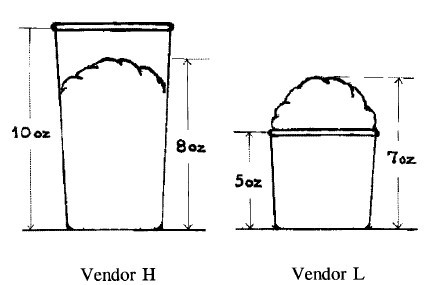
\includegraphics[scale=0.25]{Rationality20From20AI20to20Zombies2020Eliezer20Yudkowsky-img128.jpg}
 \newline
 From Hsee, © 1998 John Wiley \& Sons, Ltd.
\par}


\bigskip

{
\ \ \ ~}

{
\ \ \ Naturally, the answer depends on whether the subjects saw a single
ice cream, or the two side-by-side. Subjects who saw a single ice cream
were willing to pay \$1.66 to Vendor H and \$2.26 to Vendor L. Subjects
who saw both ice creams were willing to pay \$1.85 to Vendor H and
\$1.56 to Vendor L.}

{
\ \ \ What does this suggest for your holiday shopping? That if you
spend \$400 on a 16GB iPod Touch, your recipient sees the most
expensive MP3 player. If you spend \$400 on a Nintendo Wii, your
recipient sees the least expensive game machine. Which is better value
for the money? Ah, but that question only makes sense if you see the
two side-by-side. \textit{You'll} think about them
side-by-side while you're shopping, but the recipient
will only see what they get.}

{
\ \ \ If you have a fixed amount of money to spend---and your goal is to
display your friendship, rather than to actually \textit{help} the
recipient---you'll be better off deliberately not
shopping for value. Decide how much money you want to spend on
impressing the recipient, then find the most worthless object which
costs that amount. The cheaper the \textit{class} of objects, the more
expensive a \textit{particular} object will appear, given that you
spend a fixed amount. Which is more memorable, a \$25 shirt or a \$25
candle?}

{
\ \ \ Gives a whole new meaning to the Japanese custom of buying \$50
melons, doesn't it? You look at that and shake your
head and say ``What \textit{is} it with the
Japanese?'' And yet they get to be perceived as
incredibly generous, spendthrift even, while spending only \$50. You
could spend \$200 on a fancy dinner and not appear as wealthy as you
can by spending \$50 on a melon. If only there was a custom of gifting
\$25 toothpicks or \$10 dust specks; they could get away with spending
even less.}

{
\ \ \ PS: If you actually use this trick, I want to know what you
bought.}

{\centering
\ \ \ \ ~
\par}

{\centering
\ \ \ *
\par}


\bigskip

{
\ \ \ 1. Christopher K. Hsee, ``Less Is Better: When
Low-Value Options Are Valued More Highly than High-Value
Options,'' \textit{Behavioral Decision Making} 11 (2
1998): 107--121.}

{
\ \ \ 2. Christopher K. Hsee, ``The Evaluability
Hypothesis: An Explanation for Preference Reversals between Joint and
Separate Evaluations of Alternatives,''
\textit{Organizational Behavior and Human Decision Processes} 67 (3
1996): 247--257, doi:10.1006/obhd.1996.0077.}

{
\ \ \ 3. Slovic et al., ``Rational Actors or Rational
Fools.''}

\mysection{Unbounded Scales, Huge Jury Awards, and Futurism}

{
\ \ \ ``Psychophysics,'' despite the
name, is the respectable field that links physical effects to sensory
effects. If you dump acoustic energy into air---make noise---then
\textit{how loud} does that sound to a person, as a function of
acoustic energy? How much more acoustic energy do you have to pump into
the air, before the noise sounds twice as loud to a human listener?
It's not twice as much; more like eight times as much.
}

{
\ \ \ Acoustic energy and photons are straightforward to measure. When
you want to find out how loud an acoustic stimulus \textit{sounds}, how
bright a light source \textit{appears}, you usually ask the listener or
watcher. This can be done using a bounded scale from
``very quiet'' to
``very loud,'' or
``very dim'' to
``very bright.'' You can also use an
unbounded scale, whose zero is ``not audible at
all'' or ``not visible at
all,'' but which increases from there without limit.
When you use an unbounded scale, the observer is typically presented
with a constant stimulus, the \textit{modulus}, which is given a fixed
rating. For example, a sound that is assigned a loudness of 10. Then
the observer can indicate a sound twice as loud as the modulus by
writing 20.}

{
\ \ \ And this has proven to be a fairly reliable technique. But what
happens if you give subjects an unbounded scale, but no modulus? Zero
to infinity, with no reference point for a fixed value? Then they make
up their own modulus, of course. The \textit{ratios} between stimuli
will continue to correlate reliably between subjects. Subject A says
that sound X has a loudness of 10 and sound Y has a loudness of 15. If
subject B says that sound X has a loudness of 100, then
it's a good guess that subject B will assign loudness
in the vicinity of 150 to sound Y. But if you don't
know what subject C is using as their modulus---their scaling
factor---then there's no way to guess what subject C
will say for sound X. It could be 1. It could be 1,000.}

{
\ \ \ For a subject rating a \textit{single} sound, on an
\textit{unbounded} scale, \textit{without} a fixed standard of
comparison, nearly \textit{all} the variance is due to the arbitrary
choice of modulus, rather than the sound itself.}

{
\ \ \ ``Hm,'' you think to yourself,
``this sounds an awful lot like juries deliberating on
punitive damages. No wonder there's so much
variance!'' An interesting analogy, but how would you
go about demonstrating it experimentally?}

{
\ \ \ Kahneman et al. presented 867 jury-eligible subjects with
descriptions of legal cases (e.g., a child whose clothes caught on
fire) and asked them to either}

{
\ \ \ Rate the outrageousness of the defendant's
actions, on a bounded scale,}

{
\ \ \ Rate the degree to which the defendant should be punished, on a
bounded scale, or}

{
\ \ \ Assign a dollar value to punitive damages.\textsuperscript{1}}

{
\ \ \ And, lo and behold, while subjects correlated very well with each
other in their outrage ratings and their punishment ratings, their
punitive damages were all over the map. Yet subjects'
\textit{rank-ordering} of the punitive damages---their ordering from
lowest award to highest award---correlated well across subjects.}

{
\ \ \ If you asked how much of the variance in the
``punishment'' scale could be
explained by the specific scenario---the particular legal case, as
presented to multiple subjects---then the answer, even for the raw
scores, was 0.49. For the \textit{rank orders} of the dollar responses,
the amount of variance predicted was 0.51. For the \textit{raw dollar}
amounts, the variance explained was 0.06!}

{
\ \ \ Which is to say: if you knew the scenario presented---the
aforementioned child whose clothes caught on fire---you could take a
good guess at the punishment rating, and a good guess at the
\textit{rank-ordering} of the dollar award relative to other cases, but
the dollar award itself would be completely unpredictable.}

{
\ \ \ Taking the median of twelve randomly selected responses
didn't help much either.}

{
\ \ \ So a jury award for punitive damages isn't so much
an economic valuation as an attitude expression---a psychophysical
measure of outrage, expressed on an unbounded scale with no standard
modulus.}

{
\ \ \ I observe that many \textit{futuristic predictions} are, likewise,
best considered as attitude expressions. Take the question,
``How long will it be until we have human-level
AI?'' The responses I've seen to this
are all over the map. On one memorable occasion, a mainstream AI guy
said to me, ``Five hundred years.''
(!!)}

{
\ \ \ Now the reason why time-to-AI is just \textit{not very
predictable}, is a long discussion in its own right. But
it's not as if the guy who said ``Five
hundred years'' was looking into the future to find
out. And he can't have gotten the number using the
standard bogus method with Moore's Law. So what did the
number 500 \textit{mean}?}

{
\ \ \ As far as I can guess, it's as if
I'd asked, ``On a scale where zero is
`not difficult at all,' how difficult
does the AI problem \textit{feel} to you?'' If this
were a bounded scale, every sane respondent would mark
``extremely hard'' at the right-hand
end. Everything \textit{feels} extremely hard when you
don't know how to do it. But instead
there's an unbounded scale with no standard modulus. So
people just make up a number to represent ``extremely
difficult,'' which may come out as 50, 100, or even
500. Then they tack ``years'' on the
end, and that's their futuristic prediction.}

{
\ \ \ ``How hard does the AI problem
feel?'' isn't the only substitutable
question. Others respond as if I'd asked
``How positive do you feel about
AI?,'' except lower numbers mean more positive
feelings, and then they also tack
``years'' on the end. But if these
``time estimates'' represent
anything other than attitude expressions on an unbounded scale with no
modulus, I have been unable to determine it.}

{\centering
\ \ \ \ ~
\par}

{\centering
\ \ \ *
\par}


\bigskip

{
\ \ \ 1. Daniel Kahneman, David A. Schkade, and Cass R. Sunstein,
``Shared Outrage and Erratic Awards: The Psychology of
Punitive Damages,'' \textit{Journal of Risk and
Uncertainty} 16 (1 1998): 48--86, doi:10.1023/A:1007710408413; Daniel
Kahneman, Ilana Ritov, and David Schkade, ``Economic
Preferences or Attitude Expressions?: An Analysis of Dollar Responses
to Public Issues,'' \textit{Journal of Risk and
Uncertainty} 19, nos. 1--3 (1999): 203--235,
doi:10.1023/A:1007835629236.}

\mysection{The Halo Effect}

{
\ \ \ The affect heuristic is how an overall feeling of goodness or
badness contributes to many other judgments, whether
it's logical or not, whether you're
aware of it or not. Subjects told about the benefits of nuclear power
are likely to rate it as having fewer risks; stock analysts rating
unfamiliar stocks judge them as generally good or generally bad---low
risk and high returns, or high risk and low returns---in defiance of
ordinary economic theory, which says that risk and return should
correlate positively. }

{
\ \ \ The halo effect is the manifestation of the affect heuristic in
social psychology. Robert Cialdini, in \textit{Influence: Science and
Practice},\textsuperscript{1} summarizes:}

{
\ \ \ Research has shown that we automatically assign to good-looking
individuals such favorable traits as talent, kindness, honesty, and
intelligence (for a review of this evidence, see Eagly, Ashmore,
Makhijani, and Longo, 1991).\textsuperscript{2} Furthermore, we make
these judgments without being aware that physical attractiveness plays
a role in the process. Some consequences of this unconscious assumption
that ``good-looking equals good''
scare me. For example, a study of the 1974 Canadian federal elections
found that attractive candidates received more than two and a half
times as many votes as unattractive candidates (Efran and Patterson,
1976).\textsuperscript{3} Despite such evidence of favoritism toward
handsome politicians, follow-up research demonstrated that voters did
not realize their bias. In fact, 73 percent of Canadian voters surveyed
denied in the strongest possible terms that their votes had been
influenced by physical appearance; only 14 percent even allowed for the
possibility of such influence (Efran and Patterson,
1976).\textsuperscript{4} Voters can deny the impact of attractiveness
on electability all they want, but evidence has continued to confirm
its troubling presence (Budesheim and DePaola,
1994).\textsuperscript{5}}

{
\ \ \ A similar effect has been found in hiring situations. In one
study, good grooming of applicants in a simulated employment interview
accounted for more favorable hiring decisions than did job
qualifications---this, even though the interviewers claimed that
appearance played a small role in their choices (Mack and Rainey,
1990).\textsuperscript{6} The advantage given to attractive workers
extends past hiring day to payday. Economists examining US and Canadian
samples have found that attractive individuals get paid an average of
12--14 percent more than their unattractive coworkers (Hamermesh and
Biddle, 1994).\textsuperscript{7}}

{
\ \ \ Equally unsettling research indicates that our judicial process is
similarly susceptible to the influences of body dimensions and bone
structure. It now appears that good-looking people are likely to
receive highly favorable treatment in the legal system (see Castellow,
Wuensch, and Moore, 1991; and Downs and Lyons, 1990, for
reviews).\textsuperscript{8} For example, in a Pennsylvania study
(Stewart, 1980),\textsuperscript{9} researchers rated the physical
attractiveness of 74 separate male defendants at the start of their
criminal trials. When, much later, the researchers checked court
records for the results of these cases, they found that the handsome
men had received significantly lighter sentences. In fact, attractive
defendants were twice as likely to avoid jail as unattractive
defendants. In another study---this one on the damages awarded in a
staged negligence trial---a defendant who was better looking than his
victim was assessed an average amount of \$5,623; but when the victim
was the more attractive of the two, the average compensation was
\$10,051. What's more, both male and female jurors
exhibited the attractiveness-based favoritism (Kulka and Kessler,
1978).\textsuperscript{10}}

{
\ \ \ Other experiments have demonstrated that attractive people are
more likely to obtain help when in need (Benson, Karabenic, and Lerner,
1976)\textsuperscript{11} and are more persuasive in changing the
opinions of an audience (Chaiken, 1979) .~.~.\textsuperscript{12}}

{
\ \ \ The influence of attractiveness on ratings of intelligence,
honesty, or kindness is a clear example of bias---especially when you
judge these other qualities based on fixed text---because we
wouldn't expect judgments of honesty and attractiveness
to conflate for any legitimate reason. On the other hand, how much of
my perceived intelligence is due to my honesty? How much of my
perceived honesty is due to my intelligence? Finding the truth, and
saying the truth, are not as widely separated in nature as looking
pretty and looking smart .~.~.}

{
\ \ \ But these studies on the halo effect of attractiveness should make
us suspicious that there may be a similar halo effect for kindness, or
intelligence. Let's say that you know someone who not
only seems very intelligent, but also honest, altruistic, kindly, and
serene. You should be suspicious that some of these perceived
characteristics are influencing your perception of the others. Maybe
the person is genuinely intelligent, honest, and altruistic, but not
all that kindly or serene. You should be suspicious if the people you
know seem to separate too cleanly into devils and angels.}

{
\ \ \ And---I know you don't think \textit{you} have to
do it, but maybe \textit{you} should---be just a little more skeptical
of the more attractive political candidates.}

{\centering
\ \ \ \ ~
\par}

{\centering
\ \ \ *
\par}


\bigskip

{
\ \ \ 1. Robert B. Cialdini, \textit{Influence: Science and Practice}
(Boston: Allyn \& Bacon, 2001).}

{
\ \ \ 2. Alice H. Eagly et al., ``What Is Beautiful Is
Good, But .~.~. A Meta-analytic Review of Research on the Physical
Attractiveness Stereotype,'' \textit{Psychological
Bulletin} 110 (1 1991): 109--128, doi:10.1037/0033-2909.110.1.109.}

{
\ \ \ 3. M. G. Efran and E. W. J. Patterson, ``The
Politics of Appearance'' (Unpublished PhD thesis,
1976).}

{
\ \ \ 4. Ibid.}

{
\ \ \ 5. Thomas Lee Budesheim and Stephen DePaola,
``Beauty or the Beast?: The Effects of Appearance,
Personality, and Issue Information on Evaluations of Political
Candidates,'' \textit{Personality and Social
Psychology Bulletin} 20 (4 1994): 339--348,
doi:10.1177/0146167294204001.}

{
\ \ \ 6. Denise Mack and David Rainey, ``Female
Applicants' Grooming and Personnel
Selection,'' \textit{Journal of Social Behavior and
Personality} 5 (5 1990): 399--407.}

{
\ \ \ 7. Daniel S. Hamermesh and Jeff E. Biddle,
``Beauty and the Labor Market,''
\textit{The American Economic Review} 84 (5 1994): 1174--1194.}

{
\ \ \ 8. Wilbur A. Castellow, Karl L. Wuensch, and Charles H. Moore,
``Effects of Physical Attractiveness of the Plaintiff
and Defendant in Sexual Harassment Judgments,''
\textit{Journal of Social Behavior and Personality} 5 (6 1990):
547--562; A. Chris Downs and Phillip M. Lyons,
``Natural Observations of the Links Between
Attractiveness and Initial Legal Judgments,''
\textit{Personality and Social Psychology Bulletin} 17 (5 1991):
541--547, doi:10.1177/0146167291175009.}

{
\ \ \ 9. John E. Stewart, ``Defendants'
Attractiveness as a Factor in the Outcome of Trials: An Observational
Study,'' \textit{Journal of Applied Social
Psychology} 10 (4 1980): 348--361,
doi:10.1111/j.1559-1816.1980.tb00715.x.}

{
\ \ \ 10. Richard A. Kulka and Joan B. Kessler, ``Is
Justice Really Blind?: The Effect of Litigant Physical Attractiveness
on Judicial Judgment,'' \textit{Journal of Applied
Social Psychology} 8 (4 1978): 366--381,
doi:10.1111/j.1559-1816.1978.tb00790.x.}

{
\ \ \ 11. Peter L. Benson, Stuart A. Karabenick, and Richard M. Lerner,
``Pretty Pleases: The Effects of Physical
Attractiveness, Race, and Sex on Receiving Help,''
\textit{Journal of Experimental Social Psychology} 12 (5 1976):
409--415, doi:10.1016/0022-1031(76)90073-1.}

{
\ \ \ 12. Shelly Chaiken, ``Communicator Physical
Attractiveness and Persuasion,'' \textit{Journal of
Personality and Social Psychology} 37 (8 1979): 1387--1397,
doi:10.1037/0022-3514.37.8.1387.}

\mysection{Superhero Bias}

{
\ \ \ Suppose there's a heavily armed sociopath, a
kidnapper with hostages, who has just rejected all requests for
negotiation and announced his intent to start killing. In real life,
the good guys don't usually kick down the door when the
bad guy has hostages. But sometimes---\textit{very} rarely, but
sometimes---life imitates Hollywood to the extent of genuine good guys
needing to smash through a door. }

{
\ \ \ Imagine, in two widely separated realities, two heroes who charge
into the room, first to confront the villain.}

{
\ \ \ In one reality, the hero is strong enough to throw cars, can fire
power blasts out of his nostrils, has X-ray hearing, and his skin
doesn't just \textit{deflect} bullets but annihilates
them on contact. The villain has ensconced himself in an elementary
school and taken over two hundred children hostage; their parents are
waiting outside, weeping.}

{
\ \ \ In another reality, the hero is a New York police officer, and the
hostages are three prostitutes the villain collected off the street.}

{
\ \ \ Consider this question very carefully: Who is the greater hero?
And who is more likely to get their own comic book?}

{
\ \ \ The halo effect is that perceptions of all positive traits are
correlated. Profiles rated higher on scales of attractiveness are also
rated higher on scales of talent, kindness, honesty, and intelligence.}

{
\ \ \ And so comic-book characters who seem strong and invulnerable,
both positive traits, also seem to possess more of the heroic traits of
courage and heroism. And yet:}

{
\ \ \ How tough can it be to act all brave and courageous when
you're pretty much invulnerable?}

{\raggedleft
\ \ \ {}---Adam Warren, \textit{Empowered}, Vol. 1\textsuperscript{1}
\par}


\bigskip

{
\ \ \ I can't remember if I read the following point
somewhere, or hypothesized it myself: \textit{Fame}, in particular,
seems to combine additively with all other personality characteristics.
Consider Gandhi. Was Gandhi the \textit{most altruistic} person of the
twentieth century, or just the \textit{most famous} altruist? Gandhi
faced police with riot sticks and soldiers with guns. But Gandhi was a
celebrity, and he was protected by his celebrity. What about the others
in the march, the people who faced riot sticks and guns even though
there wouldn't be international headlines if they were
put in the hospital or gunned down?}

{
\ \ \ What did Gandhi think of getting the headlines, the celebrity, the
fame, the place in history, \textit{becoming the archetype} for
non-violent resistance, when he took less risk than any of the people
marching with him? How did he feel when one of those anonymous heroes
came up to him, eyes shining, and told Gandhi how wonderful he was? Did
Gandhi ever visualize his world in those terms? I don't
know; I'm not Gandhi.}

{
\ \ \ This is not in any sense a criticism of Gandhi. The point of
non-violent resistance is not to show off your courage. That can be
done much more easily by going over Niagara Falls in a barrel. Gandhi
couldn't help being somewhat-but-not-entirely protected
by his celebrity. And Gandhi's actions did take
courage---not as much courage as marching anonymously, but still a
great deal of courage.}

{
\ \ \ The bias I wish to point out is that Gandhi's fame
score seems to get perceptually \textit{added} to his justly
accumulated altruism score. When you think about nonviolence, you think
of Gandhi---not an anonymous protestor in one of
Gandhi's marches who faced down riot clubs and guns,
and got beaten, and had to be taken to the hospital, and walked with a
limp for the rest of her life, \textit{and no one ever remembered her
name.}}

{
\ \ \ Similarly, which is greater---to risk your life to save two
hundred children, or to risk your life to save three adults?}

{
\ \ \ The answer depends on what one means by \textit{greater.} If you
ever have to \textit{choose} between saving two hundred children and
saving three adults, then choose the former. ``Whoever
saves a single life, it is as if he had saved the whole
world'' may be a fine applause light, but
it's terrible moral advice if you've
got to pick one or the other. So if you mean
``greater'' in the sense of
``Which is more important?'' or
``Which is the preferred outcome?''
or ``Which should I choose if I have to do one or the
other?'' then it is greater to save two hundred than
three.}

{
\ \ \ But if you ask about greatness in the sense of revealed virtue,
then someone who would risk their life to save only three lives reveals
more courage than someone who would risk their life to save two hundred
but not three.}

{
\ \ \ This doesn't mean that you can deliberately choose
to risk your life to save three adults, and let the two hundred
schoolchildren go hang, because you want to reveal more virtue. Someone
who risks their life \textit{because they want to be virtuous} has
revealed far less virtue than someone who risks their life
\textit{because they want to save others}. Someone who chooses to save
three lives rather than two hundred lives, because they think it
reveals greater virtue, is so selfishly fascinated with their own
``greatness'' as to have committed
the moral equivalent of manslaughter.}

{
\ \ \ It's one of those \textit{wu wei} scenarios: You
cannot reveal virtue by trying to reveal virtue. Given a choice between
a safe method to save the world which involves no personal sacrifice or
discomfort, and a method that risks your life and requires you to
endure great privation, you cannot become a hero by deliberately
choosing the second path. There is nothing heroic about wanting to look
like a hero. It would be a lost purpose.}

{
\ \ \ Truly virtuous people who are genuinely trying to save lives,
rather than trying to reveal virtue, will constantly seek to save more
lives with less effort, which means that less of their virtue will be
revealed. It may be confusing, but it's not
contradictory.}

{
\ \ \ But we cannot always choose to be invulnerable to bullets. After
we've done our best to reduce risk and increase scope,
any \textit{remaining} heroism is well and truly revealed.}

{
\ \ \ The police officer who puts their life on the line with no
superpowers, no X-Ray vision, no super-strength, no ability to fly, and
above all no invulnerability to bullets, reveals far greater virtue
than Superman---who is a \textit{mere superhero}.}

{\centering
\ \ \ \ ~
\par}

{\centering
\ \ \ *
\par}


\bigskip

{
\ \ \ 1. Adam Warren, \textit{Empowered}, vol. 1 (Dark Horse Books,
2007).}

\mysection{Mere Messiahs}

{
\ \ \ I discussed how the halo effect, which causes people to see all
positive characteristics as correlated---for example, more attractive
individuals are also perceived as more kindly, honest, and
intelligent---causes us to admire heroes more if
they're super-strong and immune to bullets. Even
though, logically, it takes much more courage to be a hero if
you're \textit{not} immune to bullets. Furthermore, it
reveals more virtue to act courageously to save one life than to save
the world. (Although if you have to do one or the other, of course you
should save the world.) }

{
\ \ \ But let's be more specific.}

{
\ \ \ John Perry was a New York City police officer who also happened to
be an Extropian and transhumanist, which is how I come to know his
name. John Perry was due to retire shortly and start his own law
practice, when word came that a plane had slammed into the World Trade
Center. He died when the north tower fell. I didn't
know John Perry personally, so I cannot attest to this of direct
knowledge; but very few Extropians believe in God, and I expect that
Perry was likewise an atheist.}

{
\ \ \ Which is to say that Perry knew he was risking his very existence,
every week on the job. And it's not, like most people
in history, that he knew he had only a choice of how to die, and chose
to make it matter---because Perry was a transhumanist; he had genuine
hope. And Perry went out there and put his life on the line anyway. Not
because he expected any divine reward. Not because he expected to
experience anything at all, if he died. But because there were other
people in danger, and they didn't have immortal souls
either, and his hope of life was worth no more than theirs.}

{
\ \ \ I did not know John Perry. I do not know if he saw the world this
way. But the fact that an atheist and a transhumanist can still be a
police officer, can still run into the lobby of a burning building,
says more about the human spirit than all the martyrs who ever hoped of
heaven.}

{
\ \ \ So that is one specific police officer .~.~.}

{
\ \ \ .~.~. and now for the superhero.}

{
\ \ \ As the Christians tell the story, Jesus Christ could walk on
water, calm storms, drive out demons with a word. It must have made for
a comfortable life. Starvation a problem? Xerox some bread.
Don't like a tree? Curse it. Romans a problem? Sic your
Dad on them. Eventually this charmed life ended, when Jesus voluntarily
presented himself for crucifixion. Being nailed to a cross is not a
comfortable way to die. But as the Christians tell the story, Jesus did
this knowing he would come back to life three days later, and then go
to Heaven. What was the threat that moved Jesus to face this temporary
suffering followed by eternity in Heaven? Was it the life of a single
person? Was it the corruption of the church of Judea, or the oppression
of Rome? No: as the Christians tell the story, the eternal fate of
every human went on the line before Jesus suffered himself to be
temporarily nailed to a cross.}

{
\ \ \ But I do not wish to condemn a man who is not truly so guilty.
What if Jesus---no, let's pronounce his name correctly:
Yeishu---what if Yeishu of Nazareth never walked on water, and
\textit{nonetheless} defied the church of Judea established by the
powers of Rome?}

{
\ \ \ Would that not deserve greater honor than that which adheres to
Jesus Christ, who was a mere messiah?}

{
\ \ \ Alas, somehow it seems greater for a hero to have steel skin and
godlike powers. Somehow it seems to reveal more virtue to die
temporarily to save the whole world, than to die permanently
confronting a corrupt church. It seems so \textit{common}, as if many
other people through history had done the same.}

{
\ \ \ Comfortably ensconced two thousand years in the future, we can
levy all sorts of criticisms at Yeishu, but Yeishu did what he believed
to be right, confronted a church he believed to be corrupt, and died
for it. Without benefit of hindsight, he could hardly be expected to
predict the true impact of his life upon the world. Relative to most
other prophets of his day, he was probably relatively more honest,
relatively less violent, and relatively more courageous. If you strip
away the unintended consequences, the worst that can be said of Yeishu
is that others in history did better. (Epicurus, Buddha, and Marcus
Aurelius all come to mind.) Yeishu died forever, and---from one
perspective---he did it for the sake of honesty. Fifteen hundred years
before science, religious honesty was not an oxymoron.}

{
\ \ \ As Sam Harris said:\textsuperscript{1}}

{
\ \ \ It is not enough that Jesus was a man who transformed himself to
such a degree that the Sermon on the Mount could be his
heart's confession. He also had to be the Son of God,
born of a virgin, and destined to return to earth trailing clouds of
glory. The effect of such dogma is to place the example of Jesus
forever out of reach. His teaching ceases to become a set of empirical
claims about the linkage between ethics and spiritual insight and
instead becomes a gratuitous, and rather gruesome, fairy tale.
According to the dogma of Christianity, becoming just like Jesus is
impossible. One can only enumerate one's sins, believe
the unbelievable, and await the end of the world.}

{
\ \ \ I severely doubt that Yeishu ever spoke the Sermon on the Mount.
Nonetheless, Yeishu deserves honor. He deserves more honor than the
Christians would grant him.}

{
\ \ \ But since Yeishu probably anticipated his soul would survive, he
doesn't deserve more honor than John Perry.}

{\centering
\ \ \ \ ~
\par}

{\centering
\ \ \ *
\par}


\bigskip

{
\ \ \ 1. Sam Harris, \textit{The End of Faith: Religion, Terror, and the
Future of Reason} (WW Norton \& Company, 2005).}

\mysection{Affective Death Spirals}

{
\ \ \ Many, many, many are the flaws in human reasoning which lead us to
overestimate how well our beloved theory explains the facts. The
phlogiston theory of chemistry could explain just about anything, so
long as it didn't have to predict it in advance. And
the more phenomena you use your favored theory to explain, the truer
your favored theory seems---has it not been confirmed by these many
observations? As the theory seems truer, you will be more likely to
question evidence that conflicts with it. As the favored theory seems
more general, you will seek to use it in more explanations. }

{
\ \ \ If you know anyone who believes that Belgium secretly controls the
US banking system, or that they can use an invisible blue spirit force
to detect available parking spaces, that's probably how
they got started.}

{
\ \ \ (Just keep an eye out, and you'll observe much
that seems to confirm this theory .~.~.)}

{
\ \ \ This positive feedback cycle of credulity and confirmation is
indeed fearsome, and responsible for much error, both in science and in
everyday life.}

{
\ \ \ But it's nothing compared to the death spiral that
begins with a charge of positive affect---a thought that \textit{feels
really good.}}

{
\ \ \ A new political system that can save the world. A great leader,
strong and noble and wise. An amazing tonic that can cure upset
stomachs and cancer.}

{
\ \ \ Heck, why not go for all three? A great cause needs a great
leader. A great leader should be able to brew up a magical tonic or
two.}

{
\ \ \ The halo effect is that any perceived positive characteristic
(such as attractiveness or strength) increases perception of any other
positive characteristic (such as intelligence or courage). Even when it
makes no sense, or less than no sense.}

{
\ \ \ Positive characteristics enhance perception of every other
positive characteristic? That sounds a lot like how a fissioning
uranium atom sends out neutrons that fission other uranium atoms.}

{
\ \ \ Weak positive affect is subcritical; it doesn't
spiral out of control. An attractive person seems more honest, which,
perhaps, makes them seem more attractive; but the effective neutron
multiplication factor is less than one. Metaphorically speaking. The
resonance confuses things a little, but then dies out.}

{
\ \ \ With intense positive affect attached to the Great Thingy, the
resonance touches everywhere. A believing Communist sees the wisdom of
Marx in every hamburger bought at McDonald's; in every
promotion they're denied that would have gone to them
in a true worker's paradise; in every election that
doesn't go to their taste; in every newspaper article
``slanted in the wrong direction.''
Every time they use the Great Idea to interpret another event, the
Great Idea is confirmed all the more. It feels better---positive
reinforcement---and of course, when something feels good, that, alas,
makes us \textit{want} to believe it all the more.}

{
\ \ \ When the Great Thingy feels good enough to make you \textit{seek
out} new opportunities to feel even better about the Great Thingy,
applying it to interpret new events every day, the resonance of
positive affect is like a chamber full of mousetraps loaded with
ping-pong balls.}

{
\ \ \ You could call it a ``happy
attractor,'' ``overly positive
feedback,'' a ``praise locked
loop,'' or
``funpaper.'' Personally I prefer
the term ``affective death
spiral.''}

{
\ \ \ Coming up next: How to resist an affective death spiral. (Hint:
It's not by refusing to ever admire anything again, nor
by keeping the things you admire in safe little restricted
magisterium.)}

{\centering
\ \ \ \ ~
\par}

{\centering
\ \ \ *
\par}

\mysection{Resist the Happy Death Spiral}

{
\ \ \ Once upon a time, there was a man who was convinced that he
possessed a Great Idea. Indeed, as the man thought upon the Great Idea
more and more, he realized that it was not just \textit{a} great idea,
but \textit{the most wonderful idea ever}. The Great Idea would unravel
the mysteries of the universe, supersede the authority of the corrupt
and error-ridden Establishment, confer nigh-magical powers upon its
wielders, feed the hungry, heal the sick, make the whole world a better
place, etc., etc., etc. }

{
\ \ \ The man was Francis Bacon, his Great Idea was the scientific
method, and he was the only crackpot in all history to claim that level
of benefit to humanity and turn out to be completely right.}

{
\ \ \ (Bacon didn't singlehandedly invent science, of
course, but he did contribute, and may have been the first to realize
the power.)}

{
\ \ \ That's the problem with deciding that
you'll never admire anything that much: Some ideas
really \textit{are} that good. Though no one has \textit{fulfilled}
claims more audacious than Bacon's; at least, not yet.}

{
\ \ \ But then how can we resist the happy death spiral with respect to
Science itself? The happy death spiral starts when you believe
something is \textit{so} wonderful that the halo effect leads you to
find \textit{more} and \textit{more} nice things to say about it,
making you see it as \textit{even more} wonderful, and so on, spiraling
up into the abyss. What if Science is \textit{in fact} so beneficial
that we cannot acknowledge its true glory and retain our sanity? Sounds
like a nice thing to say, doesn't it? \textit{Oh no
it's starting ruuunnnnn .~.~.}}

{
\ \ \ If you retrieve the standard cached deep wisdom for
\textit{don't go overboard on admiring science}, you
will find thoughts like ``Science gave us air
conditioning, but it also made the hydrogen bomb'' or
``Science can tell us about stars and biology, but it
can never prove or disprove the dragon in my
garage.'' But the people who \textit{originated} such
thoughts were \textit{not} trying to resist a happy death spiral. They
weren't worrying about their own admiration of science
spinning out of control. Probably they didn't like
something science had to say about their pet beliefs, and sought ways
to undermine its authority.}

{
\ \ \ The \textit{standard} negative things to say about science,
aren't likely to appeal to someone who genuinely feels
the exultation of science---that's not the intended
audience. So we'll have to search for other negative
things to say instead.}

{
\ \ \ But if you look selectively for something negative to say about
science---even in an attempt to resist a happy death spiral---do you
not automatically convict yourself of rationalization? Why would you
pay attention to your own thoughts, if you knew you were trying to
manipulate yourself?}

{
\ \ \ I am generally skeptical of people who claim that one bias can be
used to counteract another. It sounds to me like an automobile mechanic
who says that the motor is broken on your right windshield wiper, but
instead of fixing it, they'll just break your left
windshield wiper to balance things out. This is the sort of cleverness
that leads to shooting yourself in the foot. Whatever the solution, it
ought to involve believing true things, rather than believing you
believe things that you believe are false.}

{
\ \ \ Can you prevent the happy death spiral by restricting your
admiration of Science to a narrow domain? Part of the happy death
spiral is seeing the Great Idea everywhere---thinking about how
Communism could cure cancer if it was only given a chance. Probably the
single most reliable sign of a cult guru is that the guru claims
expertise, not in one area, not even in a cluster of related areas, but
in \textit{everything.} The guru knows what cult members should eat,
wear, do for a living; who they should have sex with; which art they
should look at; which music they should listen to .~.~.}

{
\ \ \ Unfortunately for this plan, most people fail miserably when they
try to describe the neat little box that science has to stay inside.
The usual trick, ``Hey, science won't
cure cancer'' isn't going to fly.
``Science has nothing to say about a
parent's love for their
child''---sorry, that's simply false.
If you try to sever science from e.g. parental love, you
aren't just denying cognitive science and evolutionary
psychology. You're also denying Martine
Rothblatt's founding of United Therapeutics to seek a
cure for her daughter's pulmonary hypertension.
(Successfully, I might add.) Science is legitimately related, one way
or another, to just about every important facet of human existence.}

{
\ \ \ All right, so what's an example of a
\textit{false} nice claim you could make about science?}

{
\ \ \ In my humble opinion, one false claim is that science is so
wonderful that scientists shouldn't even try to take
ethical responsibility for their work, it will automatically end well.
This claim, to me, seems to misunderstand the nature of the process
whereby science benefits humanity. Scientists are human, they have
prosocial concerns just like most other other people, and this is at
least \textit{part} of why science ends up doing more good than evil.}

{
\ \ \ But that point is, evidently, not beyond dispute. So
here's a simpler false nice claim: ``A
cancer patient can be cured just by publishing enough journal
papers.'' Or, ``Sociopaths could
become fully normal, if they just committed themselves to never
believing anything without replicated experimental evidence with p
{\textless} 0.05.''}

{
\ \ \ The way to avoid believing such statements isn't
an affective cap, deciding that science is only slightly nice. Nor
searching for reasons to believe that publishing journal papers
\textit{causes} cancer. Nor believing that science has nothing to say
about cancer one way or the other.}

{
\ \ \ Rather, if you know with enough specificity how science works,
then you know that, while it may be possible for
``science to cure cancer,'' a cancer
patient writing journal papers isn't going to
experience a miraculous remission. That \textit{specific} proposed
chain of cause and effect is not going to work out.}

{
\ \ \ The happy death spiral is only an emotional problem because of a
perceptual problem, the halo effect, that makes us more likely to
accept future positive claims once we've accepted an
initial positive claim. We can't get rid of this effect
just by wishing; it will probably always influence us a little. But we
can manage to slow down, stop, consider each additional nice claim as
an additional burdensome detail, and focus on the specific points of
the claim apart from its positiveness.}

{
\ \ \ What if a specific nice claim
``can't be
disproven'' but there are arguments
``both for and against'' it?
Actually these are words to be wary of in general, because often this
is what people say when they're rehearsing the evidence
or avoiding the real weak points. Given the danger of the happy death
spiral, it makes sense to try to avoid being happy about
\textit{unsettled} claims---to avoid making them into a source of yet
more positive affect about something you liked already.}

{
\ \ \ The happy death spiral is only a \textit{big} emotional problem
because of the overly positive feedback, the ability for the process to
go critical. You may not be able to eliminate the halo effect entirely,
but you can apply enough critical reasoning to keep the halos
subcritical---make sure that the resonance dies out rather than
exploding.}

{
\ \ \ You might even say that the whole problem starts with people not
bothering to critically examine every additional burdensome
detail---demanding sufficient evidence to compensate for complexity,
searching for flaws as well as support, invoking curiosity---once
they've accepted some core premise. Without the
conjunction fallacy, there might still be a halo effect, but there
wouldn't be a happy death spiral.}

{
\ \ \ Even on the nicest Nice Thingies in the known universe, a perfect
rationalist who demanded exactly the necessary evidence for every
additional (positive) claim would experience no affective resonance.
You can't do this, but you can stay close enough to
rational to keep your happiness from spiraling out of control.}

{
\ \ \ The really dangerous cases are the ones where \textit{any
criticism of any positive claim about the Great Thingy feels bad or is
socially unacceptable}. Arguments are soldiers, any positive claim is a
soldier on our side, stabbing your soldiers in the back is treason.
Then the chain reaction goes \textit{super}critical. More on this
later.}

{
\ \ \ Stuart Armstrong gives closely related advice:}

{
\ \ \ Cut up your Great Thingy into smaller independent ideas,
\textit{and treat them as independent.}}

{
\ \ \ For instance a marxist would cut up Marx's Great
Thingy into a theory of value of labour, a theory of the political
relations between classes, a theory of wages, a theory on the ultimate
political state of mankind. Then each of them should be assessed
independently, and the truth or falsity of one should not halo on the
others. If we can do that, we should be safe from the spiral, as each
theory is too narrow to start a spiral on its own.}

{
\ \ \ This, metaphorically, is like keeping subcritical masses of
plutonium from coming together. Three Great Ideas are far less likely
to drive you mad than one Great Idea. Armstrong's
advice also helps promote specificity: As soon as someone says,
``Publishing enough papers can cure your
cancer,'' you ask, ``Is that a
benefit of the experimental method, and if so, at which stage of the
experimental process is the cancer cured? Or is it a benefit of science
as a social process, and if so, does it rely on individual scientists
wanting to cure cancer, or can they be
self-interested?'' Hopefully this leads you away from
the good or bad feeling, and toward noticing the confusion and lack of
support.}

{
\ \ \ To summarize, you \textit{do} avoid a Happy Death Spiral by:}

{
\ \ \ Splitting the Great Idea into parts;}

{
\ \ \ Treating every additional detail as burdensome;}

{
\ \ \ Thinking about the specifics of the causal chain instead of the
good or bad feelings;}

{
\ \ \ Not rehearsing evidence; and}

{
\ \ \ Not adding happiness from claims that ``you
can't \textit{prove} are wrong'';}

{
\ \ \ but \textit{not} by:}

{
\ \ \ Refusing to admire anything too much;}

{
\ \ \ Conducting a biased search for negative points until you feel
unhappy again; or}

{
\ \ \ Forcibly shoving an idea into a safe box.}

{\centering
\ \ \ \ ~
\par}

{\centering
\ \ \ *
\par}

\mysection{Uncritical Supercriticality}

{
\ \ \ Every now and then, you see people arguing over whether atheism is
a ``religion.'' As I touch on
elsewhere, in Purpose and Pragmatism, arguing over the meaning of a
word nearly always means that you've lost track of the
original question. How might this argument arise to begin with? }

{
\ \ \ An atheist is holding forth, blaming
``religion'' for the Inquisition,
the Crusades, and various conflicts with or within Islam. The religious
one may reply, ``But atheism is also a religion,
because you also have beliefs about God; you believe God
doesn't exist.'' Then the atheist
answers, ``If atheism is a religion, then not
collecting stamps is a hobby,'' and the argument
begins.}

{
\ \ \ Or the one may reply, ``But horrors just as great
were inflicted by Stalin, who was an atheist, and who suppressed
churches in the name of atheism; therefore you are wrong to blame the
violence on religion.'' Now the atheist may be
tempted to reply ``No true
Scotsman,'' saying,
``Stalin's religion was
Communism.'' The religious one answers
``If Communism is a religion, then Star Wars fandom is
a government,'' and the argument begins.}

{
\ \ \ Should a ``religious'' person
be defined as someone who has a definite opinion about the existence of
at least one God, e.g., assigning a probability lower than 10\% or
higher than 90\% to the existence of Zeus? Or should a
``religious'' person be defined as
someone who has a positive opinion, say a probability higher than 90\%,
for the existence of at least one God? In the former case, Stalin was
``religious''; in the latter case,
Stalin was ``not religious.''}

{
\ \ \ But this is exactly the wrong way to look at the problem. What you
really want to know---what the argument was originally about---is why,
at certain points in human history, large groups of people were
slaughtered and tortured, ostensibly in the name of an idea. Redefining
a word won't change the facts of history one way or the
other.}

{
\ \ \ Communism was a complex catastrophe, and there may be no single
\textit{why}, no single critical link in the chain of causality. But if
I had to suggest an ur-mistake, it would be .~.~. well,
I'll let God say it for me:}

{
\ \ \ If your brother, the son of your father or of your mother, or your
son or daughter, or the spouse whom you embrace, or your most intimate
friend, tries to secretly seduce you, saying, ``Let us
go and serve other gods,'' unknown to you or your
ancestors before you, gods of the peoples surrounding you, whether near
you or far away, anywhere throughout the world, you must not consent,
\textbf{you must not listen to him}; you must show him no pity, you
must not spare him or conceal his guilt. No, \textbf{you must kill
him}, your hand must strike the first blow in putting him to death and
the hands of the rest of the people following. You must stone him to
death, since he has tried to divert you from Yahweh your God.}

{\raggedleft
\ \ \ {}---Deuteronomy 13:7--11, emphasis added
\par}


\bigskip

{
\ \ \ This was likewise the rule which Stalin set for Communism, and
Hitler for Nazism: if your brother tries to tell you why Marx is wrong,
if your son tries to tell you the Jews are not planning world conquest,
then do not debate him or set forth your own evidence; do not perform
replicable experiments or examine history; but turn him in at once to
the secret police.}

{
\ \ \ I suggested that one key to resisting an affective death spiral is
the principle of ``burdensome
details''---just \textit{remembering} to question the
specific details of each additional nice claim about the Great Idea.
(It's not trivial advice. People often
don't remember to do this when they're
listening to a futurist sketching amazingly detailed projections about
the wonders of tomorrow, let alone when they're
thinking about their favorite idea ever.) This wouldn't
get rid of the halo effect, but it would hopefully reduce the resonance
to below criticality, so that one nice-sounding claim triggers less
than 1.0 additional nice-sounding claims, on average.}

{
\ \ \ The diametric opposite of this advice, which sends the halo effect
\textit{super}critical, is when it feels wrong to argue against
\textit{any} positive claim about the Great Idea. Politics is the
mind-killer. Arguments are soldiers. Once you know which side
you're on, you must support all favorable claims, and
argue against all unfavorable claims. Otherwise it's
like giving aid and comfort to the enemy, or stabbing your friends in
the back.}

{
\ \ \ If .~.~.}

{
\ \ \ .~.~. you feel that contradicting someone else who makes a flawed
nice claim in favor of evolution would be giving aid and comfort to the
creationists;}

{
\ \ \ .~.~. you feel like you get spiritual credit for each nice thing
you say about God, and arguing about it would interfere with your
relationship with God;}

{
\ \ \ .~.~. you have the distinct sense that the other people in the
room will dislike you for ``not supporting our
troops'' if you argue against the latest war;}

{
\ \ \ .~.~. saying anything against Communism gets you stoned to death
shot;}

{
\ \ \ .~.~. then the affective death spiral has gone supercritical. It
is now a Super Happy Death Spiral.}

{
\ \ \ It's not religion, as such, that is the key
categorization, relative to our original question:
``What makes the slaughter?'' The
best distinction I've heard between
``supernatural'' and
``naturalistic'' worldviews is that
a supernatural worldview asserts the existence of ontologically basic
mental substances, like spirits, while a naturalistic worldview reduces
mental phenomena to nonmental parts. Focusing on this as the source of
the problem buys into religious exceptionalism. Supernaturalist claims
are worth distinguishing, because they always turn out to be wrong for
fairly fundamental reasons. But it's still just one
kind of mistake.}

{
\ \ \ An affective death spiral can nucleate around supernatural
beliefs; especially monotheisms whose pinnacle is a Super Happy Agent,
defined primarily by agreeing with any nice statement about it;
especially meme complexes grown sophisticated enough to assert
supernatural punishments for disbelief. But the death spiral can also
start around a political innovation, a charismatic leader, belief in
racial destiny, or an economic hypothesis. The lesson of history is
that affective death spirals are dangerous whether or not they happen
to involve supernaturalism. Religion isn't special
enough, as a class of mistake, to be the key problem.}

{
\ \ \ Sam Harris came closer when he put the accusing finger on
\textit{faith.} If you don't place an appropriate
burden of proof on each and every additional nice claim, the affective
resonance gets started \textit{very} easily. Look at the poor New
Agers. Christianity developed defenses against criticism, arguing for
the wonders of faith; New Agers culturally inherit the cached thought
that faith is positive, but lack Christianity's
exclusionary scripture to keep out competing memes. New Agers end up in
happy death spirals around stars, trees, magnets, diets, spells,
unicorns .~.~.}

{
\ \ \ But the affective death spiral turns much deadlier after criticism
becomes a sin, or a gaffe, or a crime. There are things in this world
that are worth praising greatly, and you can't
\textit{flatly} say that praise beyond a certain point is forbidden.
But there is \textit{never} an Idea so true that it's
wrong to criticize any argument that supports it. Never. Never ever
never for ever. \textit{That} is flat. The vast majority of possible
beliefs in a nontrivial answer space are false, and likewise, the vast
majority of possible \textit{supporting arguments} for a true belief
are also false, and not even the happiest idea can change that.}

{
\ \ \ And it is triple ultra forbidden to respond to criticism with
violence. There are a very few injunctions in the human art of
rationality that have no ifs, ands, buts, or escape clauses. This is
one of them. Bad argument gets counterargument. Does not get bullet.
Never. Never ever never for ever.}

{\centering
\ \ \ \ ~
\par}

{\centering
\ \ \ *
\par}

\mysection{Evaporative Cooling of Group Beliefs}

{
\ \ \ Early studiers of cults were surprised to discover than when cults
receive a major shock---a prophecy fails to come true, a moral flaw of
the founder is revealed---they often come back stronger than before,
with increased belief and fanaticism. The Jehovah's
Witnesses placed Armageddon in 1975, based on Biblical calculations;
1975 has come and passed. The Unarian cult, still going strong today,
survived the nonappearance of an intergalactic spacefleet on September
27, 1975. }

{
\ \ \ Why would a group belief become \textit{stronger} after
encountering crushing counterevidence?}

{
\ \ \ The conventional interpretation of this phenomenon is based on
cognitive dissonance. When people have taken
``irrevocable'' actions in the
service of a belief---given away all their property in anticipation of
the saucers landing---they cannot possibly admit they were mistaken.
The challenge to their belief presents an immense cognitive dissonance;
they must find reinforcing thoughts to counter the shock, and so become
more fanatical. In this interpretation, the increased group fanaticism
is the result of increased individual fanaticism.}

{
\ \ \ I was looking at a Java applet which demonstrates the use of
evaporative cooling to form a Bose-Einstein condensate, when it
occurred to me that another force entirely might operate to increase
fanaticism. Evaporative cooling sets up a potential energy barrier
around a collection of hot atoms. Thermal energy is essentially
statistical in nature---not all atoms are moving at the exact same
speed. The kinetic energy of any given atom varies as the atoms collide
with each other. If you set up a potential energy barrier
that's just a little higher than the average thermal
energy, the workings of chance will give an occasional atom a kinetic
energy high enough to escape the trap. When an unusually fast atom
escapes, it takes with it an unusually large amount of kinetic energy,
and the average energy decreases. The group becomes substantially
cooler than the potential energy barrier around it. Playing with the
Java applet may make this clearer.}

{
\ \ \ In Festinger, Riecken, and Schachter's classic
\textit{When Prophecy Fails}, one of the cult members walked out the
door immediately after the flying saucer failed to
land.\textsuperscript{1} Who gets fed up and leaves \textit{first}? An
\textit{average} cult member? Or a relatively more skeptical member,
who previously might have been acting as a voice of moderation, a brake
on the more fanatic members?}

{
\ \ \ After the members with the highest kinetic energy escape, the
remaining discussions will be between the extreme fanatics on one end
and the slightly less extreme fanatics on the other end, with the group
consensus somewhere in the
``middle.''}

{
\ \ \ And what would be the analogy to collapsing to form a
Bose-Einstein condensate? Well, there's no real need to
stretch the analogy that far. But you may recall that I used a fission
chain reaction analogy for the affective death spiral; when a group
ejects all its voices of moderation, then all the people encouraging
each other, and suppressing dissents, may internally increase in
average fanaticism. (No thermodynamic analogy here, unless someone
develops a nuclear weapon that explodes when it gets cold.)}

{
\ \ \ When Ayn Rand's long-running affair with Nathaniel
Branden was revealed to the Objectivist membership, a substantial
fraction of the Objectivist membership broke off and followed Branden
into espousing an ``open system'' of
Objectivism not bound so tightly to Ayn Rand. Who stayed with Ayn Rand
even after the scandal broke? The ones who \textit{really, really}
believed in her---and perhaps some of the undecideds, who, after the
voices of moderation left, heard arguments from only one side. This may
account for how the Ayn Rand Institute is (reportedly) more fanatic
after the breakup, than the original core group of Objectivists under
Branden and Rand.}

{
\ \ \ A few years back, I was on a transhumanist mailing list where a
small group espousing ``social democratic
transhumanism'' vitriolically insulted every
libertarian on the list. Most libertarians left the mailing list, most
of the others gave up on posting. As a result, the remaining group
shifted substantially to the left. Was this deliberate? Probably not,
because I don't think the perpetrators knew that much
psychology. (For that matter, I can't recall seeing the
evaporative cooling analogy elsewhere, though that
doesn't mean it hasn't been noted
before.) At most, they might have thought to make themselves
``bigger fish in a smaller pond.''}

{
\ \ \ This is one reason why it's important to be
prejudiced in favor of tolerating dissent. Wait until substantially
\textit{after} it seems to you justified in ejecting a member from the
group, before actually ejecting. If you get rid of the old outliers,
the group position will shift, and someone else will become the
oddball. If you eject them too, you're well on the way
to becoming a Bose-Einstein condensate and, er, exploding.}

{
\ \ \ The flip side: Thomas Kuhn believed that a science has to become a
``paradigm,'' with a shared
technical language that excludes outsiders, before it can get any real
work done. In the formative stages of a science, according to Kuhn, the
adherents go to great pains to make their work comprehensible to
outside academics. But (according to Kuhn) a science can only make real
progress as a technical discipline once it abandons the requirement of
outside accessibility, and scientists working in the paradigm assume
familiarity with large cores of technical material in their
communications. This sounds cynical, relative to what is usually said
about public understanding of science, but I can definitely see a core
of truth here.}

{
\ \ \ My own theory of Internet moderation is that you have to be
willing to exclude trolls and spam to get a conversation going. You
must even be willing to exclude kindly but technically uninformed folks
from technical mailing lists if you want to get any work done. A
genuinely open conversation on the Internet degenerates fast.
It's the \textit{articulate} trolls that you should be
wary of ejecting, on this theory---they serve the hidden function of
legitimizing less extreme disagreements. But you should not have so
many articulate trolls that they begin arguing with each other, or
begin to dominate conversations. If you have one person around who is
the famous Guy Who Disagrees With Everything, anyone with a more
reasonable, more moderate disagreement won't look like
the sole nail sticking out. This theory of Internet moderation may not
have served me too well in practice, so take it with a grain of salt.}

{\centering
\ \ \ \ ~
\par}

{\centering
\ \ \ *
\par}


\bigskip

{
\ \ \ 1. Leon Festinger, Henry W. Riecken, and Stanley Schachter,
\textit{When Prophecy Fails: A Social and Psychological Study of a
Modern Group That Predicted the Destruction of the World}
(Harper-Torchbooks, 1956).}

\mysection{When None Dare Urge Restraint}

{
\ \ \ One morning, I got out of bed, turned on my computer, and my
Netscape email client automatically downloaded that
day's news pane. On that particular day, the news was
that two hijacked planes had been flown into the World Trade Center. }

{
\ \ \ These were my first three thoughts, in order:}

{
\ \ \ \textit{I guess I really am living in the Future.}}

{
\ \ \ \textit{Thank goodness it wasn't nuclear.}}

{
\ \ \ and then}

{
\ \ \ \textit{The overreaction to this will be ten times worse than the
original event.}}

{
\ \ \ A mere factor of ``ten times
worse'' turned out to be a vast understatement. Even
I didn't guess how badly things would go.
That's the challenge of pessimism; it's
\textit{really hard} to aim low enough that you're
pleasantly surprised around as often and as much as
you're unpleasantly surprised.}

{
\ \ \ Nonetheless, I did realize immediately that everyone everywhere
would be saying how awful, how terrible this event was; and that no one
would dare to be the voice of restraint, of proportionate response.
Initially, on 9/11, it was thought that six thousand people had died.
Any politician who'd said ``6,000
deaths is 1/8 the annual US casualties from automobile
accidents,'' would have been asked to resign the same
hour.}

{
\ \ \ No, 9/11 wasn't a good day. But if
\textit{everyone} gets brownie points for emphasizing how much it
hurts, and \textit{no one} dares urge restraint in how hard to hit
back, then the reaction will be greater than the appropriate level,
whatever the appropriate level may be.}

{
\ \ \ This is the even darker mirror of the happy death spiral---the
spiral of hate. Anyone who attacks the Enemy is a patriot; and whoever
tries to dissect even a single negative claim about the Enemy is a
traitor. But just as the vast majority of all complex statements are
untrue, the vast majority of negative things you can say about anyone,
even the worst person in the world, are untrue.}

{
\ \ \ I think the best illustration was ``the suicide
hijackers were cowards.'' Some common sense, please?
It takes a little courage to voluntarily fly your plane into a
building. Of all their sins, cowardice was not on the list. But I guess
anything bad you say about a terrorist, no matter how silly, must be
true. Would I get even more brownie points if I accused al-Qaeda of
having assassinated John F. Kennedy? Maybe if I accused them of being
Stalinists? Really, \textit{cowardice?}}

{
\ \ \ \textit{Yes,} it matters that the 9/11 hijackers
weren't cowards. Not just for understanding the
enemy's realistic psychology. There is simply too much
damage done by spirals of hate. It is just too dangerous for there to
be any target in the world, whether it be the Jews or Adolf Hitler,
about whom \textit{saying negative things} trumps \textit{saying
accurate things}.}

{
\ \ \ When the defense force contains thousands of aircraft and hundreds
of thousands of heavily armed soldiers, one ought to consider that the
immune system itself is capable of wreaking more damage than nineteen
guys and four nonmilitary airplanes. The US spent billions of dollars
and thousands of soldiers' lives shooting off its own
foot more effectively than any terrorist group could dream.}

{
\ \ \ If the USA had completely ignored the 9/11 attack---just shrugged
and rebuilt the building---it would have been better than the real
course of history. But that wasn't a political option.
Even if anyone privately guessed that the immune response would be more
damaging than the disease, American politicians had no
career-preserving choice but to walk straight into
al-Qaeda's trap. Whoever argues for a greater response
is a patriot. Whoever dissects a patriotic claim is a traitor.}

{
\ \ \ Initially, there were smarter responses to 9/11 than I had
guessed. I saw a Congressperson---I forget who---say in front of the
cameras, ``We have forgotten that the first purpose of
government is not the economy, it is not health care, it is defending
the country from attack.'' That widened my eyes, that
a politician could say something that wasn't an
applause light. The emotional shock must have been very great for a
Congressperson to say something that .~.~. real.}

{
\ \ \ But within two days, the genuine shock faded, and
concern-for-image regained total control of the political discourse.
Then the spiral of escalation took over completely. Once restraint
becomes unspeakable, no matter where the discourse starts out, the
level of fury and folly can only rise with time.}

{\centering
\ \ \ \ ~
\par}

{\centering
\ \ \ *
\par}

\mysection{The Robbers Cave Experiment}

{
\ \ \ Did you ever wonder, when you were a kid, whether your inane
``summer camp'' actually had some
kind of elaborate hidden purpose---say, it was all a science experiment
and the ``camp counselors'' were
really researchers observing your behavior? }

{
\ \ \ Me neither.}

{
\ \ \ But we'd have been more paranoid if
we'd read ``Intergroup Conflict and
Cooperation: The Robbers Cave Experiment'' by Sherif,
Harvey, White, Hood, and Sherif.\textsuperscript{1} In this study, the
experimental subjects---excuse me,
``campers''---were 22 boys between
fifth and sixth grade, selected from 22 different schools in Oklahoma
City, of stable middle-class Protestant families, doing well in school,
median IQ 112. They were as well-adjusted and as similar to each other
as the researchers could manage.}

{
\ \ \ The experiment, conducted in the bewildered aftermath of World War
II, was meant to investigate the causes---and possible remedies---of
intergroup conflict. How would they spark an intergroup conflict to
investigate? Well, the 22 boys were divided into two groups of 11
campers, and---}

{
\ \ \ {}---and that turned out to be quite sufficient.}

{
\ \ \ The researchers' original plans called for the
experiment to be conducted in three stages. In Stage 1, each group of
campers would settle in, unaware of the other group's
existence. Toward the end of Stage 1, the groups would gradually be
made aware of each other. In Stage 2, a set of contests and prize
competitions would set the two groups at odds.}

{
\ \ \ They needn't have bothered with Stage 2. There was
hostility almost from the moment each group became aware of the other
group's existence: They were using \textit{our}
campground, \textit{our} baseball diamond. On their first meeting, the
two groups began hurling insults. They named themselves the Rattlers
and the Eagles (they hadn't needed names when they were
the only group on the campground).}

{
\ \ \ When the contests and prizes were announced, in accordance with
pre-established experimental procedure, the intergroup rivalry rose to
a fever pitch. Good sportsmanship in the contests was evident for the
first two days but rapidly disintegrated.}

{
\ \ \ The Eagles stole the Rattlers' flag and burned it.
Rattlers raided the Eagles' cabin and stole the blue
jeans of the group leader, which they painted orange and carried as a
flag the next day, inscribed with the legend ``The
Last of the Eagles.'' The Eagles launched a
retaliatory raid on the Rattlers, turning over beds, scattering dirt.
Then they returned to their cabin where they entrenched and prepared
weapons (socks filled with rocks) in case of a return raid. After the
Eagles won the last contest planned for Stage 2, the Rattlers raided
their cabin and stole the prizes. This developed into a fistfight that
the staff had to shut down for fear of injury. The Eagles, retelling
the tale among themselves, turned the whole affair into a magnificent
victory---they'd chased the Rattlers
``over halfway back to their cabin''
(they hadn't).}

{
\ \ \ Each group developed a negative stereotype of Them and a
contrasting positive stereotype of Us. The Rattlers swore heavily. The
Eagles, after winning one game, concluded that the Eagles had won
because of their prayers and the Rattlers had lost because they used
cuss-words all the time. The Eagles decided to stop using cuss-words
themselves. They also concluded that since the Rattlers swore all the
time, it would be wiser not to talk to them. The Eagles developed an
image of themselves as proper-and-moral; the Rattlers developed an
image of themselves as rough-and-tough.}

{
\ \ \ Group members held their noses when members of the other group
passed.}

{
\ \ \ In Stage 3, the researchers tried to reduce friction between the
two groups.}

{
\ \ \ Mere contact (being present without contesting) did not reduce
friction between the two groups. Attending pleasant events
together---for example, shooting off Fourth of July fireworks---did not
reduce friction; instead it developed into a food fight.}

{
\ \ \ Would you care to guess what \textit{did} work?}

{
\ \ \ (Spoiler space .~.~.)}

{
\ \ \ The boys were informed that there might be a water shortage in the
whole camp, due to mysterious trouble with the water system---possibly
due to vandals. (The Outside Enemy, one of the oldest tricks in the
book.)}

{
\ \ \ The area between the camp and the reservoir would have to be
inspected by four search details. (Initially, these search details were
composed uniformly of members from each group.) All details would meet
up at the water tank if nothing was found. As nothing was found, the
groups met at the water tank and observed for themselves that no water
was coming from the faucet. The two groups of boys discussed where the
problem might lie, pounded the sides of the water tank, discovered a
ladder to the top, verified that the water tank was full, and finally
found the sack stuffed in the water faucet. All the boys gathered
around the faucet to clear it. Suggestions from members of both groups
were thrown at the problem and boys from both sides tried to implement
them.}

{
\ \ \ When the faucet was finally cleared, the Rattlers, who had
canteens, did not object to the Eagles taking a first turn at the
faucets (the Eagles didn't have canteens with them). No
insults were hurled, not even the customary ``Ladies
first.''}

{
\ \ \ It wasn't the end of the rivalry. There was
another food fight, with insults, the next morning. But a few more
common tasks, requiring cooperation from both groups---e.g. restarting
a stalled truck---did the job. At the end of the trip, the Rattlers
used \$5 won in a bean-toss contest to buy malts for all the boys in
both groups.}

{
\ \ \ The Robbers Cave Experiment illustrates the psychology of
hunter-gatherer bands, echoed through time, as perfectly as any
experiment ever devised by social science.}

{
\ \ \ Any resemblance to modern politics is just your imagination.}

{
\ \ \ (Sometimes I think humanity's second-greatest need
is a supervillain. Maybe I'll go into that line of work
after I finish my current job.)}

{\centering
\ \ \ \ ~
\par}

{\centering
\ \ \ *
\par}


\bigskip

{
\ \ \ 1. Muzafer Sherif et al., ``Study of Positive and
Negative Intergroup Attitudes Between Experimentally Produced Groups:
Robbers Cave Study,'' Unpublished manuscript (1954).}

\mysection{Every Cause Wants to Be a Cult}

{
\ \ \ Cade Metz at \textit{The Register} recently alleged that a secret
mailing list of Wikipedia's top administrators has
become obsessed with banning all critics and possible critics of
Wikipedia. Including banning a productive user when one
administrator---solely \textit{because} of the productivity---became
convinced that the user was a spy sent by \textit{Wikipedia Review.}
And that the top people at Wikipedia closed ranks to defend their own.
(I have not investigated these allegations myself, as yet. Hat tip to
Eugen Leitl.) }

{
\ \ \ Is there some deep moral flaw in seeking to systematize the
world's knowledge, which would lead pursuers of that
Cause into madness? Perhaps only people with innately totalitarian
tendencies would try to become the world's authority on
everything---}

{
\ \ \ Correspondence bias alert! (Correspondence bias: making inferences
about someone's unique disposition from behavior that
can be entirely explained by the situation in which it occurs. When we
see someone else kick a vending machine, we think they are
``an angry person,'' but when we
kick the vending machine, it's because the bus was
late, the train was early, and the machine ate our money.) If the
allegations about Wikipedia are true, they're explained
by \textit{ordinary} human nature, not by \textit{extraordinary} human
nature.}

{
\ \ \ The ingroup-outgroup dichotomy is part of ordinary human nature.
So are happy death spirals and spirals of hate. A Noble Cause
doesn't need a deep hidden flaw for its adherents to
form a cultish in-group. It is sufficient that the adherents be human.
Everything else follows naturally, decay by default, like food spoiling
in a refrigerator after the electricity goes off.}

{
\ \ \ In the same sense that every thermal differential wants to
equalize itself, and every computer program wants to become a
collection of ad-hoc patches, every Cause \textit{wants} to be a cult.
It's a high-entropy state into which the system trends,
an attractor in human psychology. It may have nothing to do with
whether the Cause is truly Noble. You might think that a Good Cause
would rub off its goodness on every aspect of the people associated
with it---that the Cause's followers would also be less
susceptible to status games, ingroup-outgroup bias, affective spirals,
leader-gods. But believing one true idea won't switch
off the halo effect. A noble cause won't make its
adherents something other than human. There are plenty of bad ideas
that can do plenty of damage---but that's not
necessarily what's going on.}

{
\ \ \ Every group of people with an unusual goal---good, bad, or
silly---will trend toward the cult attractor unless they make a
constant effort to resist it. You can keep your house cooler than the
outdoors, but you have to run the air conditioner constantly, and as
soon as you turn off the electricity---give up the fight against
entropy---things will go back to
``normal.''}

{
\ \ \ On one notable occasion there was a group that went semicultish
whose rallying cry was ``Rationality! Reason!
Objective reality!'' (More on this later.) Labeling
the Great Idea ``rationality''
won't protect you any more than putting up a sign over
your house that says ``Cold!'' You
still have to run the air conditioner---expend the required energy per
unit time to reverse the natural slide into cultishness. Worshipping
rationality won't make you sane any more than
worshipping gravity enables you to fly. You can't talk
to thermodynamics and you can't pray to probability
theory. You can \textit{use} it, but not join it as an in-group.}

{
\ \ \ Cultishness is quantitative, not qualitative. The question is not
``Cultish, yes or no?'' but
``How much cultishness and where?''
Even in Science, which is the archetypal Genuinely Truly Noble Cause,
we can readily point to the current frontiers of the war against
cult-entropy, where the current battle line creeps forward and back.
Are journals more likely to accept articles with a well-known authorial
byline, or from an unknown author from a well-known institution,
compared to an unknown author from an unknown institution? How much
belief is due to authority and how much is from the experiment? Which
journals are using blinded reviewers, and how effective is blinded
reviewing?}

{
\ \ \ I cite this example, rather than the standard vague accusations of
``Scientists aren't open to new
ideas,'' because it shows a \textit{battle
line}{}---a place where human psychology is being actively driven back,
where accumulated cult-entropy is being pumped out. (Of course this
requires emitting some waste heat.)}

{
\ \ \ This essay is not a catalog of techniques for actively pumping
against cultishness. Some such techniques I have said before, and some
I will say later. \textit{Here} I just want to point out that the
worthiness of the Cause does not mean you can spend any \textit{less}
effort in resisting the cult attractor. And that if you can point to
current battle lines, it does not mean you confess your Noble Cause
unworthy. You might think that if the question were
``Cultish, yes or no?'' that you
were obliged to answer ``No,'' or
else betray your beloved Cause. But that is like thinking that you
should divide engines into ``perfectly
efficient'' and
``inefficient,'' instead of
measuring waste.}

{
\ \ \ Contrariwise, if you believe that it was the Inherent Impurity of
those Foolish Other Causes that made them go wrong, if you laugh at the
folly of ``cult victims,'' if you
think that cults are led and populated by mutants, then you will not
expend the necessary effort to pump against entropy---to resist being
human.}

{\centering
\ \ \ \ ~
\par}

{\centering
\ \ \ *
\par}

\mysection{Guardians of the Truth}

{
\ \ \ The criticism is sometimes leveled against rationalists:
``The Inquisition thought \textit{they} had the truth!
Clearly this `truth' business is
dangerous.'' }

{
\ \ \ There are many obvious responses, such as ``If
you think that possessing the truth \textit{would} license you to
torture and kill, you're making a mistake that has
nothing to do with epistemology.'' Or,
``So that historical statement you just made about the
Inquisition---is it true?''}

{
\ \ \ Reversed stupidity is not intelligence: ``If your
current computer stops working, you can't conclude that
everything about the current system is wrong and that you need a new
system without an AMD processor, an ATI video card .~.~. even though
your current system has all these things and it doesn't
work. Maybe you just need a new power cord.'' To
arrive at a poor conclusion requires only one wrong step, not every
step wrong. The Inquisitors believed that 2 + 2 = 4, but that
wasn't the source of their madness. Maybe
epistemological realism wasn't the problem either?}

{
\ \ \ It does seem plausible that if the Inquisition had been made up of
relativists, professing that nothing was true and nothing mattered,
they would have mustered less enthusiasm for their torture. They would
also have been less enthusiastic if lobotomized. I think
that's a fair analogy.}

{
\ \ \ And yet .~.~. I think the Inquisition's attitude
toward truth played a role. The Inquisition believed that there was
such a thing as truth, and that it was important; well, likewise
Richard Feynman. But the Inquisitors were not Truth-Seekers. They were
Truth-\textit{Guardians.}}

{
\ \ \ I once read an argument (I can't find the source)
that a key component of a \textit{zeitgeist} is whether it locates its
ideals in its future or its past. Nearly all cultures before the
Enlightenment believed in a Fall from Grace---that things had once been
perfect in the distant past, but then catastrophe had struck, and
everything had slowly run downhill since then:}

{
\ \ \ In the age when life on Earth was full .~.~. They loved each other
and did not know that this was ``love of
neighbor.'' They deceived no one yet they did not
know that they were ``men to be
trusted.'' They were reliable and did not know that
this was ``good faith.'' They lived
freely together giving and taking, and did not know that they were
generous. For this reason their deeds have not been narrated. They made
no history.}

{\raggedleft
\ \ \ {}---\textit{The Way of Chuang Tzu}, trans. Thomas
Merton\textsuperscript{1}
\par}


\bigskip

{
\ \ \ The perfect age of the past, according to our best anthropological
evidence, never existed. But a culture that sees life running
inexorably downward is very different from a culture in which you can
reach unprecedented heights.}

{
\ \ \ (I say ``culture,'' and not
``society,'' because you can have
more than one subculture in a society.)}

{
\ \ \ You could say that the difference between e.g. Richard Feynman and
the Inquisition was that the Inquisition believed they \textit{had}
truth, while Richard Feynman \textit{sought} truth. This
isn't quite defensible, though, because there were
undoubtedly some truths that Richard Feynman thought he \textit{had} as
well. ``The sky is blue,'' for
example, or ``2 + 2 = 4.''}

{
\ \ \ Yes, there are effectively certain truths of science. General
Relativity may be overturned by some future physics---albeit not in any
way that predicts the Sun will orbit Jupiter; the new theory must steal
the successful predictions of the old theory, not contradict them. But
evolutionary theory takes place on a higher level of organization than
atoms, and nothing we discover about quarks is going to throw out
Darwinism, or the cell theory of biology, or the atomic theory of
chemistry, or a hundred other brilliant innovations whose truth is now
established beyond \textit{reasonable} doubt.}

{
\ \ \ Are these ``absolute truths''?
Not in the sense of possessing a probability of literally 1.0. But they
are cases where science basically thinks it's got the
truth.}

{
\ \ \ And yet scientists don't torture people who
question the atomic theory of chemistry. Why not? Because they
don't believe that certainty licenses torture? Well,
yes, that's the \textit{surface} difference; but why
\textit{don't} scientists believe this?}

{
\ \ \ Because chemistry asserts no supernatural penalty of eternal
torture for disbelieving in the atomic theory of chemistry? But again
we recurse and ask the question,
``Why?'' Why
\textit{don't} chemists believe that you go to hell if
you disbelieve in the atomic theory?}

{
\ \ \ Because journals won't publish your paper until
you get a solid experimental observation of Hell? But all too many
scientists can suppress their skeptical reflex at will. Why
don't chemists have a private cult which argues that
nonchemists go to hell, given that many are Christians anyway?}

{
\ \ \ Questions like that don't have neat single-factor
answers. But I would argue that \textit{one} of the factors has to do
with assuming a \textit{productive} posture toward the truth, versus a
\textit{defensive} posture toward the truth.}

{
\ \ \ When you are the Guardian of the Truth, you've got
nothing useful to contribute to the Truth \textit{but} your
guardianship of it. When you're trying to win the Nobel
Prize in chemistry by discovering the next benzene or buckyball,
someone who challenges the atomic theory isn't so much
a threat to your worldview as a waste of your time.}

{
\ \ \ When you are a Guardian of the Truth, all you can do is try to
stave off the inevitable slide into entropy by zapping anything that
departs from the Truth. If there's some way to pump
against entropy, generate new true beliefs along with a little waste
heat, that same pump can keep the truth alive without secret police. In
chemistry you can replicate experiments and see for yourself---and that
keeps the precious truth alive without need of violence.}

{
\ \ \ And it's not such a terrible threat if we make one
mistake somewhere---end up believing a little untruth for a little
while---because \textit{tomorrow} we can recover the lost ground.}

{
\ \ \ But this whole trick only works because the experimental method is
a ``criterion of goodness'' which is
not a mere ``criterion of
comparison.'' Because experiments can recover the
truth without need of authority, they can also \textit{override}
authority and create new true beliefs where none existed before.}

{
\ \ \ Where there are criteria of goodness that are not criteria of
comparison, there can exist \textit{changes} which are
\textit{improvements}, rather than \textit{threats.} Where there are
\textit{only} criteria of comparison, where there's no
way to move past authority, there's also no way to
resolve a disagreement between authorities. Except extermination. The
bigger guns win.}

{
\ \ \ I don't mean to provide a grand overarching
single-factor view of history. I do mean to point out a deep
psychological difference between seeing your grand cause in life as
\textit{protecting, guarding, preserving}, versus \textit{discovering,
creating, improving}. Does the
``up'' direction of time point to
the past or the future? It's a distinction that shades
everything, casts tendrils everywhere.}

{
\ \ \ This is why I've always insisted, for example,
that if you're going to start talking about
``AI ethics,'' you had better be
talking about how you are going to \textit{improve} on the current
situation using AI, rather than just keeping various things from going
wrong. Once you adopt criteria of mere comparison, you start losing
track of your ideals---lose sight of wrong and right, and start seeing
simply ``different'' and
``same.''}

{
\ \ \ I would also argue that this basic psychological difference is one
of the reasons why an academic field that stops making active progress
tends to turn \textit{mean.} (At least by the refined standards of
science. \textit{Reputational} assassination is tame by historical
standards; most defensive-posture belief systems went for the real
thing.) If major shakeups don't arrive often enough to
regularly promote young scientists based on merit rather than
conformity, the field stops resisting the standard degeneration into
authority. When there's not many discoveries being
made, there's nothing left to do all day but witch-hunt
the heretics.}

{
\ \ \ To get the best mental health benefits of the
discover/create/improve posture, you've got to
\textit{actually be making progress}, not just hoping for it.}

{\centering
\ \ \ \ ~
\par}

{\centering
\ \ \ *
\par}


\bigskip

{
\ \ \ 1. Zhuangzi and Thomas Merton, \textit{The Way of Chuang Tzu} (New
Directions Publishing, 1965).}

\mysection{Guardians of the Gene Pool}

{
\ \ \ Like any educated denizen of the twenty-first century, you may
have heard of World War II. You may remember that Hitler and the Nazis
planned to carry forward a romanticized process of evolution, to breed
a new master race, supermen, stronger and smarter than anything that
had existed before. }

{
\ \ \ Actually this is a common misconception. Hitler believed that the
Aryan superman \textit{had previously existed}{}---the Nordic
stereotype, the blond blue-eyed beast of prey---but had been
\textit{polluted} by mingling with impure races. There had been a
racial Fall from Grace.}

{
\ \ \ It says something about the degree to which the concept of
\textit{progress} permeates Western civilization, that the one is told
about Nazi eugenics and hears ``They tried to breed a
superhuman.'' \textit{You,} dear reader---if
\textit{you} failed so hard that you endorsed coercive eugenics,
\textit{you} would try to create a superhuman. Because you locate your
ideals in your future, not in your past. Because you are
\textit{creative.} The thought of breeding back to some Nordic
archetype from a thousand years earlier would not even occur to you as
a possibility---what, just the \textit{Vikings?} That's
\textit{all?} If you failed hard enough to kill, you would damn well
try to reach heights never before reached, or what a waste it would all
be, eh? Well, that's one reason you're
not a Nazi, dear reader.}

{
\ \ \ It says something about how difficult it is for the relatively
healthy to envision themselves in the shoes of the relatively sick,
that we are told of the Nazis, and distort the tale to make them
defective transhumanists.}

{
\ \ \ It's the \textit{Communists} who were the
defective transhumanists. ``New Soviet
Man'' and all that. The Nazis were quite definitely
the bioconservatives of the tale.}

{\centering
\ \ \ \ ~
\par}

{\centering
\ \ \ *
\par}

\mysection{Guardians of Ayn Rand}

{
\ \ \ For skeptics, the idea that reason can lead to a cult is absurd.
The characteristics of a cult are 180 degrees out of phase with reason.
But as I will demonstrate, not only can it happen, it has happened, and
to a group that would have to be considered the unlikeliest cult in
history. It is a lesson in what happens when the truth becomes more
important than the search for truth .~.~.}

{\raggedleft
\ \ \ {}---Michael Shermer, ``The Unlikeliest Cult in
History''\textsuperscript{1}
\par}


\bigskip

{
\ \ \ ~}

{
\ \ \ I think Michael Shermer is over-explaining Objectivism.
I'll get around to amplifying on that.}

{
\ \ \ Ayn Rand's novels glorify technology, capitalism,
individual defiance of the System, limited government, private
property, selfishness. Her ultimate fictional hero, John Galt, was
{\textless}SPOILER{\textgreater} a scientist who invented a new form of
cheap renewable energy; but then refuses to give it to the world since
the profits will only be stolen to prop up corrupt
governments.{\textless}/SPOILER{\textgreater}}

{
\ \ \ And then---somehow---it all turned into a moral and philosophical
``closed system'' with Ayn Rand at
the center. The term ``closed
system'' is not my own accusation;
it's the term the Ayn Rand Institute uses to describe
Objectivism. Objectivism is defined by the works of Ayn Rand. Now that
Rand is dead, Objectivism is closed. If you disagree with
Rand's works in any respect, you cannot be an
Objectivist.}

{
\ \ \ Max Gluckman once said: ``A science is any
discipline in which the fool of this generation can go beyond the point
reached by the genius of the last generation.''
Science moves forward by slaying its heroes, as Newton fell to
Einstein. Every young physicist dreams of being the new champion that
future physicists will dream of dethroning.}

{
\ \ \ Ayn Rand's philosophical idol was Aristotle. Now
maybe Aristotle was a hot young math talent 2,350 years ago, but math
has made noticeable progress since his day. Bayesian probability theory
is the quantitative logic of which Aristotle's
qualitative logic is a special case; but there's no
sign that Ayn Rand knew about Bayesian probability theory when she
wrote her magnum opus, \textit{Atlas Shrugged.} Rand wrote about
``rationality,'' yet failed to
familiarize herself with the modern research in heuristics and biases.
How can anyone claim to be a master rationalist, yet know nothing of
such elementary subjects?}

{
\ \ \ ``Wait a minute,'' objects the
reader, ``that's not quite fair!
\textit{Atlas Shrugged} was published in 1957! Practically nobody knew
about Bayes back then.'' Bah. Next
you'll tell me that Ayn Rand died in 1982, and had no
chance to read \textit{Judgment Under Uncertainty: Heuristics and
Biases}, which was published that same year.}

{
\ \ \ Science isn't fair. That's sorta
the point. An aspiring rationalist in 2007 starts with a huge advantage
over an aspiring rationalist in 1957. It's how we know
that progress has occurred.}

{
\ \ \ To me the thought of voluntarily embracing a system explicitly
tied to the beliefs of one human being, who's
\textit{dead}, falls somewhere between the silly and the suicidal. A
computer isn't five years old before
it's obsolete.}

{
\ \ \ The vibrance that Rand admired in science, in commerce, in every
railroad that replaced a horse-and-buggy route, in every skyscraper
built with \textit{new} architecture---it all comes from the principle
of \textit{surpassing the ancient masters.} How can there be science,
if the most knowledgeable scientist there will ever be, has already
lived? Who would raise the New York skyline that Rand admired so, if
the tallest building that would ever exist, had already been built?}

{
\ \ \ And yet Ayn Rand acknowledged no superior, in the past, or in the
future yet to come. Rand, who began in admiring reason and
individuality, ended by ostracizing anyone who dared contradict her.
Shermer:}

{
\ \ \ [Barbara] Branden recalled an evening when a friend of
Rand's remarked that he enjoyed the music of Richard
Strauss. ``When he left at the end of the evening, Ayn
said, in a reaction becoming increasingly typical, `Now
I understand why he and I can never be real soulmates. The distance in
our sense of life is too great.'''
Often she did not wait until a friend had left to make such remarks.}

{
\ \ \ Ayn Rand changed over time, one suspects.}

{
\ \ \ Rand grew up in Russia, and witnessed the Bolshevik revolution
firsthand. She was granted a visa to visit American relatives at the
age of 21, and she never returned. It's easy to hate
authoritarianism when you're the victim.
It's easy to champion the freedom of the individual,
when you are yourself the oppressed.}

{
\ \ \ It takes a much stronger constitution to fear authority when
\textit{you} have the power. When people are looking to \textit{you}
for answers, it's harder to say ``What
the hell do I know about music? I'm a writer, not a
composer,'' or
``It's hard to see how liking a piece
of music can be untrue.''}

{
\ \ \ When \textit{you're} the one crushing those who
dare offend you, the exercise of power somehow seems much more
\textit{justifiable} than when you're the one being
crushed. All sorts of excellent justifications somehow leap to mind.}

{
\ \ \ Michael Shermer goes into detail on how he thinks that
Rand's philosophy ended up descending into cultishness.
In particular, Shermer says (it seems) that Objectivism failed because
Rand thought that certainty was possible, while science is never
certain. I can't back Shermer on that one. The atomic
theory of chemistry is pretty damned certain. But chemists
haven't become a cult.}

{
\ \ \ Actually, I think Shermer's falling prey to
correspondence bias by supposing that there's any
particular correlation between Rand's philosophy and
the way her followers formed a cult. Every cause wants to be a cult.}

{
\ \ \ Ayn Rand fled the Soviet Union, wrote a book about individualism
that a lot of people liked, got plenty of compliments, and formed a
coterie of admirers. Her admirers found nicer and nicer things to say
about her (happy death spiral), and she enjoyed it too much to tell
them to shut up. She found herself with the power to crush those of
whom she disapproved, and she didn't resist the
temptation of power.}

{
\ \ \ Ayn Rand and Nathaniel Branden carried on a secret extramarital
affair. (With permission from both their spouses, which counts for a
lot in my view. If you want to turn that into a
``problem,'' you have to specify
that the spouses were \textit{unhappy}{}---and then
it's still not a matter for outsiders.) When Branden
was revealed to have ``cheated'' on
Rand with yet another woman, Rand flew into a fury and excommunicated
him. Many Objectivists broke away when news of the affair became
public.}

{
\ \ \ Who stayed with Rand, rather than following Branden, or leaving
Objectivism altogether? Her \textit{strongest} supporters. Who
departed? The previous voices of moderation. (Evaporative cooling of
group beliefs.) Ever after, Rand's grip over her
remaining coterie was absolute, and no questioning was allowed.}

{
\ \ \ The only extraordinary thing about the whole business, is how
ordinary it was.}

{
\ \ \ You might think that a belief system which praised
``reason'' and
``rationality'' and
``individualism'' would have gained
some kind of special immunity, somehow .~.~. ?}

{
\ \ \ Well, it didn't.}

{
\ \ \ It worked around as well as putting a sign saying
``Cold'' on a refrigerator that
wasn't plugged in.}

{
\ \ \ The active effort required to resist the slide into entropy
wasn't there, and decay inevitably followed.}

{
\ \ \ And if you call that the ``unlikeliest cult in
history,'' you're just calling
reality nasty names.}

{
\ \ \ Let that be a lesson to all of us: Praising
``rationality'' counts for nothing.
Even saying ``You must justify your beliefs through
Reason, not by agreeing with the Great Leader'' just
runs a little automatic program that takes whatever the Great Leader
says and generates a justification that your fellow followers will view
as Reason-able.}

{
\ \ \ So where is the true art of rationality to be found? Studying up
on the math of probability theory and decision theory. Absorbing the
cognitive sciences like evolutionary psychology, or heuristics and
biases. Reading history books .~.~.}

{
\ \ \ ``Study science, not just me!''
is probably the most important piece of advice Ayn Rand
should've given her followers and
didn't. There's no one human being who
ever lived, whose shoulders were broad enough to bear \textit{all} the
weight of a true science with many contributors.}

{
\ \ \ It's noteworthy, I think, that Ayn
Rand's fictional heroes were architects and engineers;
John Galt, her ultimate, was a physicist; and yet Ayn Rand herself
wasn't a great scientist. As far as I know, she
wasn't particularly good at math. She could not aspire
to rival her own heroes. Maybe that's why she began to
lose track of the will to keep improving herself.}

{
\ \ \ Now me, y'know, I admire Francis
Bacon's audacity, but I retain my ability to bashfully
confess, ``If I could go back in time, and somehow
make Francis Bacon understand the problem I'm currently
working on, his eyeballs would pop out of their sockets like champagne
corks and explode.''}

{
\ \ \ I admire Newton's accomplishments. But my attitude
toward a woman's right to vote bars me from accepting
Newton as a moral paragon. Just as my knowledge of Bayesian probability
bars me from viewing Newton as the ultimate unbeatable source of
mathematical knowledge. And my knowledge of Special Relativity, paltry
and little-used though it may be, bars me from viewing Newton as the
ultimate authority on physics.}

{
\ \ \ Newton couldn't realistically have discovered any
of the ideas I'm lording over him---\textit{but
progress isn't fair! That's the
point!}}

{
\ \ \ Science has heroes, but no gods. The great Names are not our
superiors, or even our rivals; they are passed milestones on our road.
And the most important milestone is the hero yet to come.}

{
\ \ \ To be one more milestone in humanity's road is the
best that can be said of anyone; but this seemed too lowly to please
Ayn Rand. And that is how she became a mere Ultimate Prophet.}

{\centering
\ \ \ \ ~
\par}

{\centering
\ \ \ *
\par}


\bigskip

{
\ \ \ 1. Michael Shermer, ``The Unlikeliest Cult in
History,'' \textit{Skeptic} 2, no. 2 (1993): 74--81,
http://www.2think.org/02\_2\_she.shtml.}

\mysection{Two Cult Koans}

{
\ \ \ A novice rationalist studying under the master Ougi was rebuked by
a friend who said, ``You spend all this time listening
to your master, and talking of
`rational' this and
`rational' that---you have fallen into a
cult!'' }

{
\ \ \ The novice was deeply disturbed; he heard the words,
``You have fallen into a cult!''
resounding in his ears as he lay in bed that night, and even in his
dreams.}

{
\ \ \ The next day, the novice approached Ougi and related the events,
and said, ``Master, I am constantly consumed by worry
that this is all really a cult, and that your teachings are only
dogma.''}

{
\ \ \ Ougi replied, ``If you find a hammer lying in the
road and sell it, you may ask a low price or a high one. But if you
keep the hammer and use it to drive nails, who can doubt its
worth?''}

{
\ \ \ The novice said, ``See, now
that's just the sort of thing I worry about---your
mysterious Zen replies.''}

{
\ \ \ Ougi said, ``Fine, then, I will speak more
plainly, and lay out perfectly reasonable arguments which demonstrate
that you have not fallen into a cult. But first you have to wear this
silly hat.''}

{
\ \ \ Ougi gave the novice a huge brown ten-gallon cowboy hat.}

{
\ \ \ ``Er, master .~.~.'' said the
novice.}

{
\ \ \ ``When I have explained everything to
you,'' said Ougi, ``you will see why
this was necessary. Or otherwise, you can continue to lie awake nights,
wondering whether this is a cult.''}

{
\ \ \ The novice put on the cowboy hat.}

{
\ \ \ Ougi said, ``How long will you repeat my words
and ignore the meaning? Disordered thoughts begin as feelings of
attachment to preferred conclusions. You are too anxious about your
self-image as a rationalist. You came to me to seek reassurance. If you
had been truly curious, not knowing one way or the other, you would
have thought of ways to resolve your doubts. Because you needed to
resolve your cognitive dissonance, you were willing to put on a silly
hat. If I had been an evil man, I could have made you pay a hundred
silver coins. When you concentrate on a real-world question, the worth
or worthlessness of your understanding will soon become apparent. You
are like a swordsman who keeps glancing away to see if anyone might be
laughing at him---''}

{
\ \ \ ``All \textit{right},'' said
the novice.}

{
\ \ \ ``You asked for the long
version,'' said Ougi.}

{
\ \ \ This novice later succeeded Ougi and became known as Ni no Tachi.
Ever after, he would not allow his students to cite his words in their
debates, saying, ``Use the techniques and do not
mention them.''}

{
\ \ \ A novice rationalist approached the master Ougi and said,
``Master, I worry that our rationality dojo is .~.~.
well .~.~. a little cultish.''}

{
\ \ \ ``That is a grave concern,''
said Ougi.}

{
\ \ \ The novice waited a time, but Ougi said nothing more.}

{
\ \ \ So the novice spoke up again: ``I mean,
I'm sorry, but having to wear these robes, and the
hood---it just seems like we're the bloody Freemasons
or something.''}

{
\ \ \ ``Ah,'' said Ougi,
``the robes and trappings.''}

{
\ \ \ ``Well, \textit{yes} the robes and
trappings,'' said the novice. ``It
just seems terribly irrational.''}

{
\ \ \ ``I will address all your
concerns,'' said the master, ``but
first you must put on this silly hat.'' And Ougi drew
out a wizard's hat, embroidered with crescents and
stars.}

{
\ \ \ The novice took the hat, looked at it, and then burst out in
frustration: ``\textit{How can this possibly
help?}''}

{
\ \ \ ``Since you are so concerned about the
interactions of clothing with probability theory,''
Ougi said, ``it should not surprise you that you must
wear a special hat to understand.''}

{
\ \ \ When the novice attained the rank of grad student, he took the
name Bouzo and would only discuss rationality while wearing a clown
suit.}

{\centering
\ \ \ \ ~
\par}

{\centering
\ \ \ *
\par}

\mysection{Asch's Conformity Experiment}

{
\ \ \  
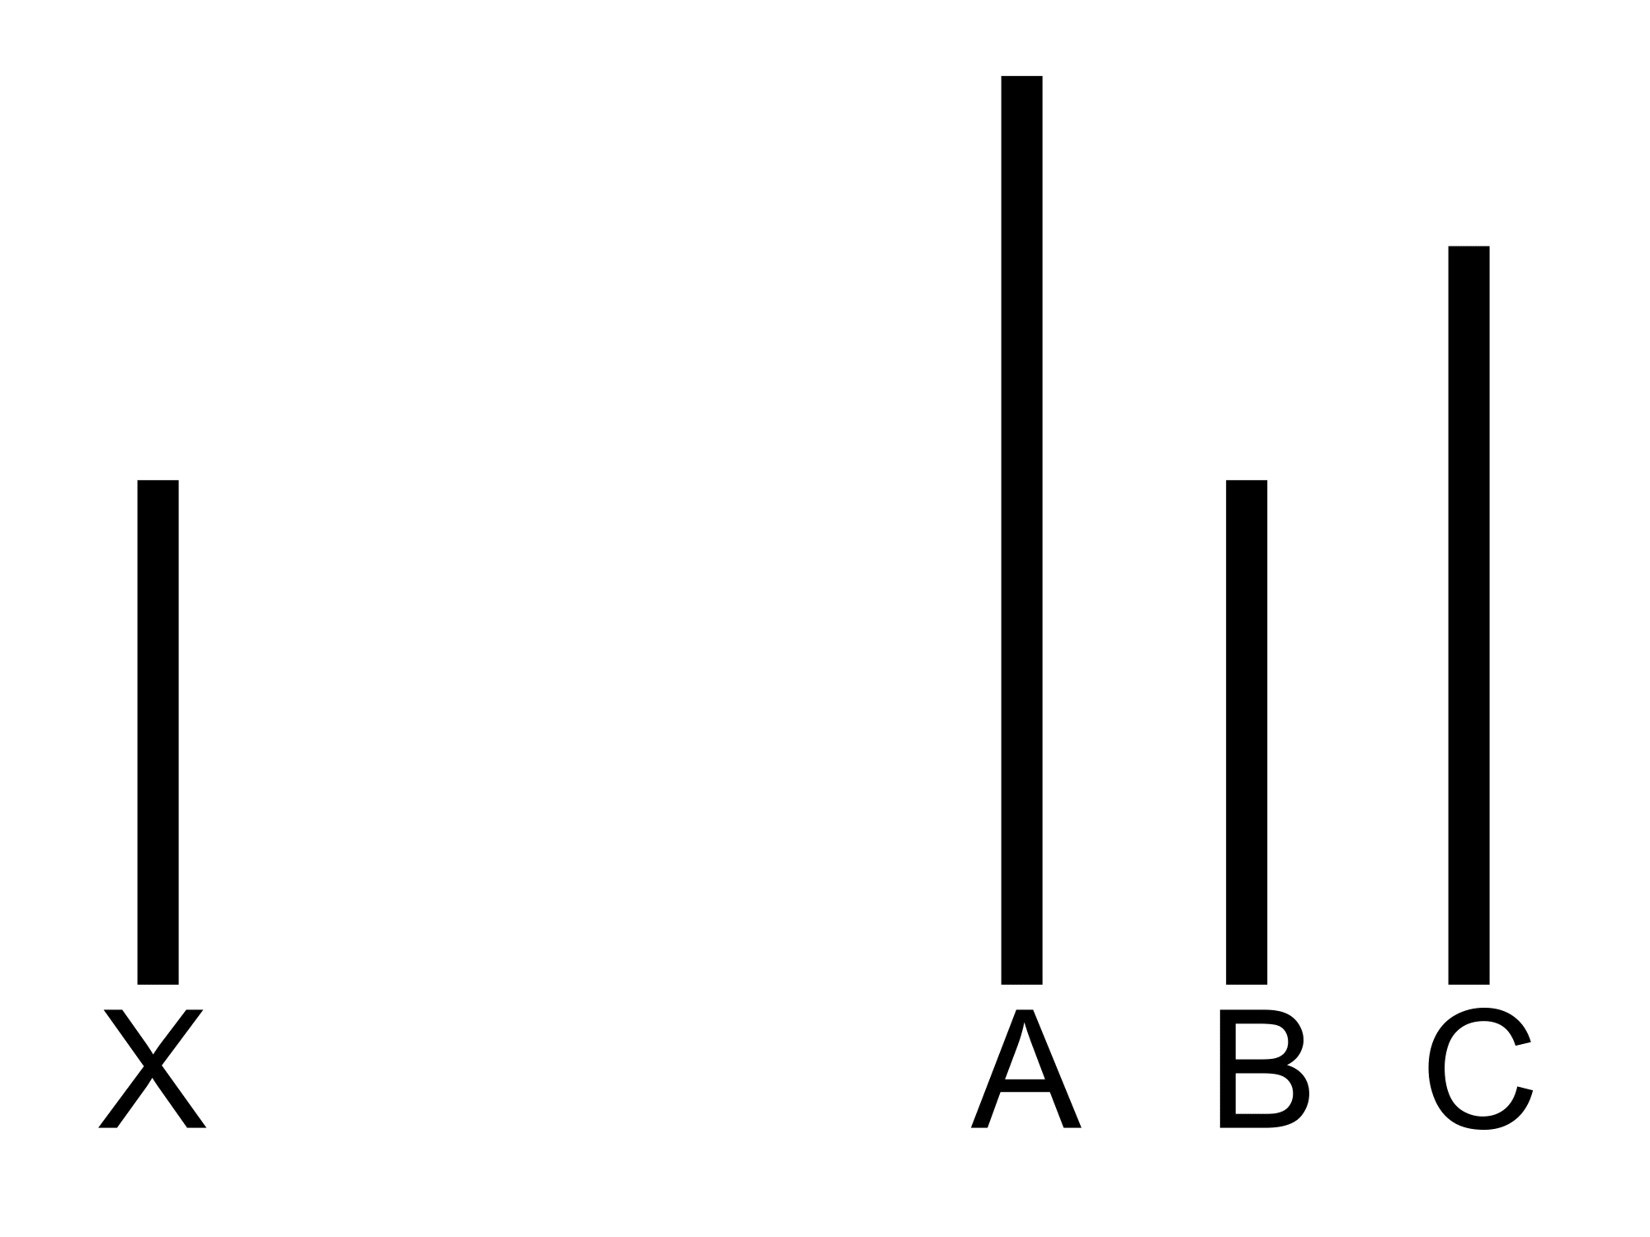
\includegraphics[scale=0.25]{Rationality20From20AI20to20Zombies2020Eliezer20Yudkowsky-img145.jpg}
 }

{
\ \ \ ~}

{
\ \ \ Solomon Asch, with experiments originally carried out in the 1950s
and well-replicated since, highlighted a phenomenon now known as
``conformity.'' In the classic
experiment, a subject sees a puzzle like the one in the nearby diagram:
Which of the lines A, B, and C is the same size as the line X? Take a
moment to determine your own answer .~.~.}

{
\ \ \ The gotcha is that the subject is seated alongside a number of
other people looking at the diagram---seemingly other subjects,
actually confederates of the experimenter. The other
``subjects'' in the experiment, one
after the other, say that line C seems to be the same size as X. The
real subject is seated next-to-last. How many people, placed in this
situation, would say ``C''---giving
an obviously incorrect answer that agrees with the unanimous answer of
the other subjects? What do you think the percentage would be?}

{
\ \ \ Three-quarters of the subjects in Asch's
experiment gave a ``conforming''
answer at least once. A third of the subjects conformed more than half
the time.}

{
\ \ \ Interviews after the experiment showed that while most subjects
claimed to have not really believed their conforming answers, some said
they'd really thought that the conforming option was
the correct one.}

{
\ \ \ Asch was disturbed by these results:}

{
\ \ \ That we have found the tendency to conformity in our society so
strong .~.~. is a matter of concern. It raises questions about our ways
of education and about the values that guide our
conduct.\textsuperscript{1}}

{
\ \ \ It is not a trivial question whether the subjects of
Asch's experiments behaved \textit{irrationally.}
Robert Aumann's Agreement Theorem shows that honest
Bayesians cannot agree to disagree---if they have common knowledge of
their probability estimates, they have the same probability estimate.
Aumann's Agreement Theorem was proved more than twenty
years after Asch's experiments, but it only formalizes
and strengthens an intuitively obvious point---other
people's beliefs are often legitimate evidence.}

{
\ \ \ If you were looking at a diagram like the one above, but you knew
\textit{for a fact} that the other people in the experiment were honest
and seeing the same diagram as you, and three other people said that C
was the same size as X, then what are the odds that \textit{only you}
are the one who's right? I lay claim to no advantage of
\textit{visual} reasoning---I don't think
I'm better than an average human at judging whether two
lines are the same size. In terms of individual rationality, I hope I
would notice my own severe confusion and then assign {\textgreater}50\%
probability to the majority vote.}

{
\ \ \ In terms of group rationality, seems to me that the proper thing
for an honest rationalist to say is, ``How surprising,
it \textit{looks} to me like B is the same size as X. But if
we're all looking at the same diagram and reporting
honestly, I have no reason to believe that my assessment is better than
yours.'' The last sentence is
important---it's a much weaker claim of disagreement
than, ``Oh, \textit{I} see the optical illusion---I
understand why you think it's C, of course, but the
real answer is B.''}

{
\ \ \ So the conforming subjects in these experiments are not
\textit{automatically} convicted of irrationality, based on what
I've described so far. But as you might expect, the
devil is in the details of the experimental results. According to a
meta-analysis of over a hundred replications by Smith and
Bond:\textsuperscript{2}}

{
\ \ \ Conformity increases strongly up to 3 confederates, but
doesn't increase further up to 10--15 confederates. If
people are conforming rationally, then the opinion of 15 other subjects
should be substantially stronger evidence than the opinion of 3 other
subjects.}

{
\ \ \ Adding a single dissenter---just one other person who gives the
correct answer, or even an incorrect answer that's
different from the group's incorrect answer---reduces
conformity \textit{very} sharply, down to 5--10\% of subjects. If
you're applying some intuitive version of
Aumann's Agreement to think that when 1 person
disagrees with 3 people, the 3 are probably right, then in most cases
you should be equally willing to think that 2 people will disagree with
6 people. (Not automatically true, but true \textit{ceteris paribus}.)
On the other hand, if you've got people who are
emotionally nervous about being the odd one out, then
it's easy to see how a single other person who agrees
with you, or even a single other person who disagrees with the group,
would make you much less nervous.}

{
\ \ \ Unsurprisingly, subjects in the one-dissenter condition did not
think their nonconformity had been influenced or enabled by the
dissenter. Like the 90\% of drivers who think they're
above-average in the top 50\%, some of them may be right about this,
but not all. People are not self-aware of the causes of their
conformity or dissent, which weighs against trying to argue them as
manifestations of rationality. For example, in the hypothesis that
people are socially-rationally choosing to lie in order to not stick
out, it appears that (at least some) subjects in the one-dissenter
condition do not consciously anticipate the
``conscious strategy'' they would
employ when faced with unanimous opposition.}

{
\ \ \ When the single dissenter suddenly switched to \textit{conforming
to the group}, subjects' conformity rates went back up
to just as high as in the no-dissenter condition. Being the first
dissenter is a valuable (and costly!) social service, but
you've got to keep it up.}

{
\ \ \ Consistently within and across experiments, all-female groups (a
female subject alongside female confederates) conform significantly
more often than all-male groups. Around one-half the women conform more
than half the time, versus a third of the men. If you argue that the
average subject is rational, then apparently women are too agreeable
and men are too disagreeable, so neither group is actually
\textit{rational} .~.~.}

{
\ \ \ Ingroup-outgroup manipulations (e.g., a handicapped subject
alongside other handicapped subjects) similarly show that conformity is
significantly higher among members of an ingroup.}

{
\ \ \ Conformity is lower in the case of blatant diagrams, like the one
at the beginning of this essay, versus diagrams where the errors are
more subtle. This is hard to explain if (all) the subjects are making a
socially rational decision to avoid sticking out.}

{
\ \ \ Paul Crowley reminds me to note that when subjects can respond in
a way that will not be seen by the group, conformity also drops, which
also argues against an Aumann interpretation.}

{\centering
\ \ \ \ ~
\par}

{\centering
\ \ \ *
\par}


\bigskip

{
\ \ \ 1. Solomon E. Asch, ``Studies of Independence and
Conformity: A Minority of One Against a Unanimous
Majority,'' \textit{Psychological Monographs} 70
(1956).}

{
\ \ \ 2. Rod Bond and Peter B. Smith, ``Culture and
Conformity: A Meta-Analysis of Studies Using Asch's
(1952b, 1956) Line Judgment Task,''
\textit{Psychological Bulletin} 119 (1996): 111--137.}

\mysection{On Expressing Your Concerns}

{
\ \ \ The scary thing about Asch's conformity
experiments is that you can get many people to say black is white, if
you put them in a room full of other people saying the same thing. The
hopeful thing about Asch's conformity experiments is
that a single dissenter tremendously drove down the rate of conformity,
even if the dissenter was only giving a different wrong answer. And the
\textit{wearisome} thing is that dissent was not \textit{learned} over
the course of the experiment---when the single dissenter started siding
with the group, rates of conformity rose back up. }

{
\ \ \ Being a voice of dissent can bring real benefits to the group. But
it also (famously) has a cost. And then you have to keep it up. Plus
you could be wrong.}

{
\ \ \ I recently had an interesting experience wherein I began
discussing a project with two people who had previously done some
planning on their own. I thought they were being too optimistic and
made a number of safety-margin-type suggestions for the project. Soon a
fourth guy wandered by, who was providing one of the other two with a
ride home, and began making suggestions. At this point I had a sudden
insight about how groups become overconfident, because whenever I
raised a possible problem, the fourth guy would say,
``Don't worry, I'm
sure we can handle it!'' or something similarly
reassuring.}

{
\ \ \ An individual, working alone, will have natural doubts. They will
think to themselves ``Can I really do
XYZ?,'' because there's nothing
impolite about doubting your \textit{own} competence. But when two
unconfident people form a group, it is polite to say nice and
reassuring things, and impolite to question the other
person's competence. Together they become more
optimistic than either would be on their own, each
one's doubts quelled by the other's
seemingly confident reassurance, not realizing that the other person
initially had the same inner doubts.}

{
\ \ \ The most fearsome possibility raised by Asch's
experiments on conformity is the specter of everyone agreeing with the
group, swayed by the confident voices of others, careful not to let
their own doubts show---not realizing that others are suppressing
similar worries. This is known as ``pluralistic
ignorance.''}

{
\ \ \ Robin Hanson and I have a long-running debate over when, exactly,
aspiring rationalists should dare to disagree. I tend toward the widely
held position that you have no real choice but to form your own
opinions. Robin Hanson advocates a more iconoclastic position, that
\textit{you}{}---not just other people---should consider that others
may be wiser. Regardless of our various disputes, we both agree that
Aumann's Agreement Theorem extends to imply that common
knowledge of a factual disagreement shows \textit{someone} must be
irrational. Despite the funny looks we've gotten,
we're sticking to our guns about modesty: Forget what
everyone tells you about individualism, you \textit{should} pay
attention to what other people think.}

{
\ \ \ Ahem. The point is that, for rationalists, disagreeing with the
group is serious business. You can't wave it off with
``Everyone is entitled to their own
opinion.''}

{
\ \ \ I think the most important lesson to take away from
Asch's experiments is to distinguish
``expressing concern'' from
``disagreement.'' Raising a point
that others haven't voiced is not a promise to disagree
with the group at the end of its discussion.}

{
\ \ \ The ideal Bayesian's process of convergence
involves sharing evidence that is unpredictable to the listener. The
Aumann agreement result holds only for \textit{common knowledge}, where
you know, I know, you know I know, etc. Hanson's post
or paper on ``We Can't Foresee to
Disagree'' provides a picture of how strange it would
look to watch ideal rationalists converging on a probability estimate;
it doesn't look anything like two bargainers in a
marketplace converging on a price.}

{
\ \ \ Unfortunately, there's not much difference
\textit{socially} between ``expressing
concerns'' and
``disagreement.'' A group of
rationalists might agree to pretend there's a
difference, but it's not how human beings are really
wired. Once you speak out, you've committed a socially
irrevocable act; you've become the nail sticking up,
the discord in the comfortable group harmony, and you
can't undo that. Anyone insulted by a concern you
expressed about their competence to successfully complete task XYZ,
will probably hold just as much of a grudge afterward if you say
``No problem, I'll go along with the
group'' at the end.}

{
\ \ \ Asch's experiment shows that the power of dissent
to inspire others is real. Asch's experiment shows that
the power of conformity is real. If everyone refrains from voicing
their private doubts, that will indeed lead groups into madness. But
history abounds with lessons on the price of being the first, or even
the second, to say that the Emperor has no clothes. Nor are people
hardwired to distinguish ``expressing a
concern'' from ``disagreement even
with common knowledge''; this distinction is a
rationalist's artifice. If you read the more cynical
brand of self-help books (e.g., Machiavelli's
\textit{The Prince}) they will advise you to mask your nonconformity
entirely, \textit{not} voice your concerns first and then agree at the
end. If you perform the group service of being the one who gives voice
to the obvious problems, don't expect the group to
thank you for it.}

{
\ \ \ These are the costs and the benefits of dissenting---whether you
``disagree'' or just
``express concern''---and the
decision is up to you.}

{\centering
\ \ \ \ ~
\par}

{\centering
\ \ \ *
\par}

\mysection{Lonely Dissent}

{
\ \ \ Asch's conformity experiment showed that the
presence of a single dissenter tremendously reduced the incidence of
``conforming'' wrong answers.
Individualism is easy, experiment shows, when you have company in your
defiance. Every other subject in the room, except one, says that black
is white. You become the second person to say that black is black. And
it feels glorious: the two of you, lonely and defiant rebels, against
the world! (Followup interviews showed that subjects in the
one-dissenter condition expressed strong feelings of camaraderie with
the dissenter---though, of course, they didn't think
the presence of the dissenter had influenced their own nonconformity.)
}

{
\ \ \ But you can only \textit{join} the rebellion, after someone,
somewhere, becomes the \textit{first} to rebel. Someone has to say that
black is black after hearing \textit{everyone} else, one after the
other, say that black is white. And that---experiment shows---is a
\textit{lot harder.}}

{
\ \ \ Lonely dissent doesn't feel like going to school
dressed in black. It feels like going to school wearing a clown suit.}

{
\ \ \ That's the difference between \textit{joining the
rebellion} and \textit{leaving the pack}.}

{
\ \ \ If there's one thing I can't
stand, it's fakeness---you may have noticed this. Well,
lonely dissent has got to be one of the most commonly, most
ostentatiously faked characteristics around. Everyone wants to be an
iconoclast.}

{
\ \ \ I don't mean to degrade the act of joining a
rebellion. There are rebellions worth joining. It does take courage to
brave the disapproval of your peer group, or perhaps even worse, their
shrugs. Needless to say, going to a rock concert is not rebellion. But,
for example, vegetarianism is. I'm not a vegetarian
myself, but I respect people who are, because I expect it takes a
noticeable amount of quiet courage to tell people that hamburgers
won't work for dinner. (Albeit that in the Bay Area,
people ask as a matter of routine.)}

{
\ \ \ Still, if you tell people that you're a
vegetarian, they'll think they understand your motives
(even if they don't). They may disagree. They may be
offended if you manage to announce it proudly enough, or for that
matter, they may be offended just because they're
easily offended. But they know how to relate to you.}

{
\ \ \ When someone wears black to school, the teachers and the other
children understand the role thereby being assumed in their society.
It's Outside the System---in a very standard way that
everyone recognizes and understands. Not, y'know,
\textit{actually} outside the system. It's a Challenge
to Standard Thinking, of a standard sort, so that people indignantly
say ``I can't understand why
you---'' but don't have to actually
think any thoughts they had not thought before. As the saying goes,
``Has any of the `subversive
literature' you've read caused you to
modify any of your political views?''}

{
\ \ \ What takes \textit{real} courage is braving the outright
\textit{incomprehension} of the people around you, when you do
something that \textit{isn't} Standard Rebellion \#37,
something for which they lack a ready-made script. They
don't hate you for a rebel, they just think
you're, like, weird, and turn away. This prospect
generates a much deeper fear. It's the difference
between explaining vegetarianism and explaining cryonics. There are
other cryonicists in the world, somewhere, but they
aren't there next to you. You have to explain it,
alone, to people who just think it's \textit{weird}.
Not forbidden, but outside bounds that people don't
even think about. You're going to get your head frozen?
You think that's going to stop you from dying? What do
you mean, brain information? Huh? What? Are you \textit{crazy?}}

{
\ \ \ I'm tempted to essay a post facto explanation in
evolutionary psychology: You could get together with a small group of
friends and walk away from your hunter-gatherer band, but having to go
it \textit{alone} in the forests was probably a death sentence---at
least reproductively. We don't reason this out
explicitly, but that is not the nature of evolutionary psychology.
Joining a rebellion that everyone knows about is scary, but nowhere
near as scary as doing something really differently. Something that in
ancestral times might have ended up, not with the band splitting, but
with you being driven out alone.}

{
\ \ \ As the case of cryonics testifies, the fear of thinking
\textit{really} different is stronger than the fear of death.
Hunter-gatherers had to be ready to face death on a routine basis,
hunting large mammals, or just walking around in a world that contained
predators. They needed that courage in order to live. Courage to defy
the tribe's standard ways of thinking, to entertain
thoughts that seem truly weird---well, that probably
didn't serve its bearers as well. We
don't reason this out explicitly;
that's not how evolutionary psychology works. We human
beings are just built in such fashion that many more of us go skydiving
than sign up for cryonics.}

{
\ \ \ And that's not even the highest courage.
There's more than one cryonicist in the world. Only
Robert Ettinger had to say it \textit{first.}}

{
\ \ \ To be a \textit{scientific} revolutionary, you've
got to be the first person to contradict what everyone else you know is
thinking. This is not the only route to scientific greatness; it is
rare even among the great. No one can become a scientific revolutionary
by trying to imitate revolutionariness. You can only get there by
pursuing the correct answer in all things, whether the correct answer
is revolutionary or not. But if, in the due course of time---if, having
absorbed all the power and wisdom of the knowledge that has already
accumulated---if, after all that and a dose of sheer luck, you find
your pursuit of mere correctness taking you into new territory .~.~.
\textit{then} you have an opportunity for your courage to fail.}

{
\ \ \ This is the true courage of lonely dissent, which every damn rock
band out there tries to fake.}

{
\ \ \ Of course not everything that takes courage is a good idea. It
would take courage to walk off a cliff, but then you would just go
splat.}

{
\ \ \ The \textit{fear} of lonely dissent is a hindrance to good ideas,
but not every dissenting idea is good. See also Robin
Hanson's Against Free Thinkers. Most of the difficulty
in having a new true scientific thought is in the
``true'' part.}

{
\ \ \ It really isn't \textit{necessary} to be different
for the sake of being different. If you do things differently only when
you see an overwhelmingly good reason, you will have more than enough
trouble to last you the rest of your life.}

{
\ \ \ There are a few genuine packs of iconoclasts around. The Church of
the SubGenius, for example, seems to genuinely aim at
\textit{confusing} the mundanes, not merely offending them. And there
are islands of genuine tolerance in the world, such as science fiction
conventions. There \textit{are} certain people who have no fear of
departing the pack. Many fewer such people really exist, than imagine
themselves rebels; but they do exist. And yet scientific
revolutionaries are tremendously rarer. Ponder that.}

{
\ \ \ Now \textit{me}, you know, I \textit{really am} an iconoclast.
Everyone thinks they are, but with me it's
\textit{true}, you see. I would \textit{totally} have worn a clown suit
to school. My serious conversations were with books, not with other
children.}

{
\ \ \ But if you think you would \textit{totally} wear that clown suit,
then don't be too proud of that either! It just means
that you need to make an effort in the \textit{opposite direction} to
avoid dissenting too easily. That's what I have to do,
to correct for my own nature. Other people do have reasons for thinking
what they do, and ignoring that completely is as bad as being afraid to
contradict them. You wouldn't want to end up as a free
thinker. It's not a \textit{virtue}, you see---just a
bias either way.}

{\centering
\ \ \ \ ~
\par}

{\centering
\ \ \ *
\par}

\mysection{Cultish Countercultishness}

{
\ \ \ In the modern world, joining a cult is probably one of the worse
things that can happen to you. The best-case scenario is that
you'll end up in a group of sincere but deluded people,
making an honest mistake but otherwise well-behaved, and
you'll spend a lot of time and money but end up with
nothing to show. Actually, that could describe any failed Silicon
Valley startup. Which is supposed to be a hell of a harrowing
experience, come to think. So yes, very scary. }

{
\ \ \ Real cults are vastly worse. ``Love
bombing'' as a recruitment technique, targeted at
people going through a personal crisis. Sleep deprivation. Induced
fatigue from hard labor. Distant communes to isolate the recruit from
friends and family. Daily meetings to confess impure thoughts.
It's not unusual for cults to take \textit{all} the
recruit's money---life savings plus weekly
paycheck---forcing them to depend on the cult for food and clothing.
Starvation as a punishment for disobedience. Serious brainwashing and
serious harm.}

{
\ \ \ With all that taken into account, I should probably sympathize
more with people who are terribly nervous, embarking on some
odd-seeming endeavor, that \textit{they might be joining a cult.} It
should not grate on my nerves. Which it does.}

{
\ \ \ Point one: ``Cults'' and
``non-cults'' aren't
separated natural kinds like dogs and cats. If you look at any list of
cult characteristics, you'll see items that could
easily describe political parties and
corporations---``group members encouraged to distrust
outside criticism as having hidden motives,''
``hierarchical authoritative
structure.'' I've written on group
failure modes like group polarization, happy death spirals,
uncriticality, and evaporative cooling, all of which seem to feed on
each other. When these failures swirl together and meet, they combine
to form a Super-Failure stupider than any of the parts, like Voltron.
But this is not a cult \textit{essence}; it is a cult
\textit{attractor.}}

{
\ \ \ Dogs are born with dog DNA, and cats are born with cat DNA. In the
current world, there is no in-between. (Even with genetic manipulation,
it wouldn't be as simple as creating an organism with
half dog genes and half cat genes.) It's not like
there's a mutually reinforcing set of
dog-characteristics, which an individual cat can wander halfway into
and become a semidog.}

{
\ \ \ The human mind, as it thinks about categories, seems to prefer
essences to attractors. The one wishes to say ``It is
a cult'' or ``It is not a
cult,'' and then the task of classification is over
and done. If you observe that Socrates has ten fingers, wears clothes,
and speaks fluent Greek, then you can say ``Socrates
is human'' and from there deduce
``Socrates is vulnerable to
hemlock'' without doing specific blood tests to
confirm his mortality. You have decided Socrates's
humanness once and for all.}

{
\ \ \ But if you observe that a certain group of people seems to exhibit
ingroup-outgroup polarization and see a positive halo effect around
their Favorite Thing Ever---which could be Objectivism, or
vegetarianism, or neural networks{}---you cannot, \textit{from the
evidence gathered so far,} deduce whether they have achieved
uncriticality. You cannot deduce whether their main idea is true, or
false, or genuinely useful but not quite as useful as they think.
\textit{From the information gathered so far}, you cannot deduce
whether they are otherwise polite, or if they will lure you into
isolation and deprive you of sleep and food. The characteristics of
cultness are not all present or all absent.}

{
\ \ \ If you look at online arguments over ``X is a
cult,'' ``X is not a
cult,'' then one side goes through an online list of
cult characteristics and finds one that applies and says
``Therefore it is a cult!'' And the
defender finds a characteristic that does not apply and says
``Therefore it is not a cult!''}

{
\ \ \ You cannot build up an accurate picture of a
group's reasoning dynamic using this kind of
essentialism. You've got to pay attention to individual
characteristics individually.}

{
\ \ \ Furthermore, reversed stupidity is not intelligence. If
you're interested in the central \textit{idea}, not
just the implementation group, then smart ideas can have stupid
followers. Lots of New Agers talk about ``quantum
physics'' but this is no strike against quantum
physics. Of course stupid ideas can also have stupid followers. Along
with binary essentialism goes the idea that if you infer that a group
is a ``cult,'' therefore their
beliefs must be false, because false beliefs are characteristic of
cults, just like cats have fur. If you're interested in
the idea, then look at the idea, not the people. Cultishness is a
characteristic of \textit{groups} more than \textit{hypotheses.}}

{
\ \ \ The second error is that when people nervously ask,
``This isn't a cult, is
it?,'' it sounds to me like they're
seeking \textit{reassurance of rationality.} The notion of a
rationalist not getting too attached to their self-image as a
rationalist deserves its own essay (though see Twelve Virtues, Why
Truth? And .~.~., and Two Cult Koans). But even without going into
detail, surely one can see that \textit{nervously seeking reassurance}
is not the best frame of mind in which to evaluate questions of
rationality. You will not be genuinely curious or think of ways to
fulfill your doubts. Instead, you'll find some online
source which says that cults use sleep deprivation to control people,
you'll notice that Your-Favorite-Group
doesn't use sleep deprivation, and
you'll conclude ``It's
not a cult. Whew!'' If it doesn't
have fur, it must not be a cat. Very reassuring.}

{
\ \ \ But Every Cause Wants To Be A Cult, whether the cause itself is
wise or foolish. The ingroup-outgroup dichotomy etc. are part of human
nature, not a special curse of mutants. Rationality is the exception,
not the rule. You have to put forth a constant effort to maintain
rationality against the natural slide into entropy. If you decide
``It's not a cult!''
and sigh with relief, then you will not put forth a continuing effort
to push back \textit{ordinary} tendencies toward cultishness.
You'll decide the cult-essence is absent, and stop
pumping against the entropy of the cult-attractor.}

{
\ \ \ If you are terribly nervous about cultishness, then you will want
to deny any hint of any characteristic that resembles a cult. But
\textit{any} group with a goal seen in a positive light is at risk for
the halo effect, and will have to pump against entropy to avoid an
affective death spiral. This is true even for ordinary institutions
like political parties---people who think that
``liberal values'' or
``conservative values'' can cure
cancer, etc. It is true for Silicon Valley startups, both failed and
successful. It is true of Mac users and of Linux users. The halo effect
doesn't become okay just because everyone does it; if
everyone walks off a cliff, you wouldn't too. The error
in reasoning is to be fought, not tolerated. But if
you're too nervous about ``Are you
\textit{sure} this isn't a cult?''
then you will be reluctant to see \textit{any} sign of cultishness,
because that would imply you're in a cult, and
\textit{It's not a cult!!} So you won't
see the current battlefields where the \textit{ordinary} tendencies
toward cultishness are creeping forward, or being pushed back.}

{
\ \ \ The third mistake in nervously asking ``This
isn't a cult, is it?'' is that, I
strongly suspect, the \textit{nervousness} is there for entirely the
wrong reasons.}

{
\ \ \ Why is it that groups which praise their Happy Thing to the stars,
encourage members to donate all their money and work in voluntary
servitude, and run private compounds in which members are kept tightly
secluded, are called ``religions''
rather than ``cults'' once
they've been around for a few hundred years?}

{
\ \ \ Why is it that most of the people who nervously ask of cryonics,
``This isn't a cult, is
it?'' would not be equally nervous about attending a
Republican or Democrat political rally? Ingroup-outgroup dichotomies
and happy death spirals can happen in political discussion, in
mainstream religions, in sports fandom. If the \textit{nervousness}
came from fear of \textit{rationality errors}, people would ask
``This isn't an ingroup-outgroup
dichotomy, is it?'' about Democrat or Republican
political rallies, in just the same fearful tones.}

{
\ \ \ There's a legitimate reason to be less fearful of
Libertarianism than of a flying-saucer cult, because Libertarians
don't have a reputation for employing sleep deprivation
to convert people. But cryonicists don't have a
reputation for using sleep deprivation, either. So why be any more
worried about having your head frozen after you stop breathing?}

{
\ \ \ I suspect that the \textit{nervousness} is not the fear of
believing falsely, or the fear of physical harm. It is the fear of
lonely dissent. The nervous feeling that subjects get in
Asch's conformity experiment, when all the other
subjects (actually confederates) say one after another that line C is
the same size as line X, and it looks to the subject like line B is the
same size as line X. The fear of leaving the pack.}

{
\ \ \ That's why groups whose beliefs have been around
long enough to seem ``normal''
don't inspire the same nervousness as
``cults,'' though some mainstream
religions may also take all your money and send you to a monastery.
It's why groups like political parties, that are
strongly liable for rationality errors, don't inspire
the same nervousness as ``cults.''
The word ``cult''
isn't being used to symbolize rationality errors,
it's being used as a label for something that
\textit{seems weird.}}

{
\ \ \ Not every change is an improvement, but every improvement is
necessarily a change. That which you want to do better, you have no
choice but to do differently. Common wisdom does embody a fair amount
of, well, actual wisdom; yes, it makes sense to require an extra burden
of proof for weirdness. But the \textit{nervousness}
isn't that kind of deliberate, rational consideration.
It's the fear of believing something that will make
your friends look at you really oddly. And so people ask
``This isn't a \textit{cult}, is
it?'' in a tone that they would never use for
attending a political rally, or for putting up a gigantic Christmas
display.}

{
\ \ \ \textit{That's} the part that bugs me.}

{
\ \ \ It's as if, as soon as you believe anything that
your ancestors did not believe, the Cult Fairy comes down from the sky
and infuses you with the Essence of Cultness, and the next thing you
know, you're all wearing robes and chanting. As if
``weird'' beliefs are the
\textit{direct cause} of the problems, never mind the sleep deprivation
and beatings. The harm done by cults---the Heaven's
Gate suicide and so on---just goes to show that everyone with an odd
belief is crazy; the first and foremost characteristic of
``cult members'' is that they are
Outsiders with Peculiar Ways.}

{
\ \ \ Yes, socially unusual belief puts a group at risk for
ingroup-outgroup thinking and evaporative cooling and other problems.
But the unusualness is a risk factor, not a disease in itself. Same
thing with having a goal that you think is worth accomplishing. Whether
or not the belief is true, having a nice goal always puts you at risk
of the happy death spiral. But that makes lofty goals a risk factor,
not a disease. Some goals are genuinely worth pursuing.}

{
\ \ \ On the other hand, I see no legitimate reason for sleep
deprivation or threatening dissenters with beating, full stop. When a
group does this, then whether you call it
``cult'' or
``not-cult,'' you have directly
answered the pragmatic question of whether to join.}

{
\ \ \ Problem four: The fear of lonely dissent is something that
\textit{cults themselves} exploit. Being afraid of your friends looking
at you disapprovingly is \textit{exactly the effect that real cults use
to convert and keep members---}surrounding converts with wall-to-wall
agreement among cult believers.}

{
\ \ \ The fear of strange ideas, the impulse to conformity, has no doubt
warned many potential victims away from flying-saucer cults. When
you're out, it keeps you out. But when
you're \textit{in}, it keeps you \textit{in.}
Conformity just glues you to wherever you are, whether
that's a good place or a bad place.}

{
\ \ \ The one wishes there was some way they could be \textit{sure} that
they weren't in a
``cult.'' Some definite, crushing
rejoinder to people who looked at them funny. Some way they could know
once and for all that they were doing the right thing, without these
constant doubts. I believe that's called
``need for closure.'' And---of
course---cults exploit that, too.}

{
\ \ \ Hence the phrase, ``Cultish
countercultishness.''}

{
\ \ \ Living with doubt is not a virtue---the purpose of every doubt is
to annihilate itself in success or failure, and a doubt that just hangs
around accomplishes nothing. But sometimes a doubt does take a while to
annihilate itself. Living with a stack of currently unresolved doubts
is an unavoidable fact of life for rationalists. Doubt
shouldn't be scary. Otherwise you're
going to have to choose between living one heck of a hunted life, or
one heck of a stupid one.}

{
\ \ \ If you really, genuinely can't figure out whether
a group is a ``cult,'' then
you'll just have to choose under conditions of
uncertainty. That's what decision theory is all about.}

{
\ \ \ Problem five: Lack of strategic thinking.}

{
\ \ \ I know people who are cautious around Singularitarianism, and
they're \textit{also} cautious around political parties
and mainstream religions. \textit{Cautious,} not nervous or defensive.
These people can see at a glance that Singularitarianism is obviously
not a full-blown cult with sleep deprivation etc. But they worry that
Singularitarianism will \textit{become} a cult, because of risk factors
like turning the concept of a powerful AI into a Super Happy Agent (an
agent defined primarily by agreeing with any nice thing said about it).
Just because something isn't a cult now,
doesn't mean it won't become a cult in
the future. Cultishness is an attractor, not an essence.}

{
\ \ \ Does \textit{this} kind of caution annoy me? Hell no. I spend a
lot of time worrying about that scenario myself. I try to place my Go
stones in advance to block movement in that direction. Hence, for
example, the series of essays on cultish failures of reasoning.}

{
\ \ \ People who talk about
``rationality'' also have an added
risk factor. Giving people advice about how to think is an inherently
dangerous business. But it is a \textit{risk factor}, not a
\textit{disease.}}

{
\ \ \ Both of my favorite Causes are at-risk for cultishness. Yet
somehow, I get asked ``Are you sure this
isn't a cult?'' a lot more often when
I talk about powerful AIs, than when I talk about probability theory
and cognitive science. I don't know if one risk factor
is higher than the other, but I know which one \textit{sounds weirder}
.~.~.}

{
\ \ \ Problem \#6 with asking ``This
isn't a cult, is it?'' .~.~.}

{
\ \ \ Just the question itself places me in a very annoying sort of
Catch-22. An actual Evil Guru would surely use the
one's nervousness against them, and design a plausible
elaborate argument explaining Why This Is Not A Cult, and the one would
be eager to accept it. Sometimes I get the impression that this is what
people \textit{want} me to do! Whenever I try to write about
cultishness and how to avoid it, I keep feeling like
I'm giving in to that flawed desire---that I am, in the
end, providing people with \textit{reassurance.} Even when I tell
people that a constant fight against entropy is required.}

{
\ \ \ It feels like I'm making myself a first dissenter
in Asch's conformity experiment, telling people,
``Yes, line X really is the same as line B,
it's okay for you to say so too.''
They shouldn't need to ask! Or, even worse, it feels
like I'm presenting an elaborate argument for Why This
Is Not A Cult. It's a \textit{wrong question.}}

{
\ \ \ Just look at the group's reasoning processes for
yourself, and decide for yourself whether it's
something you want to be part of, once you get rid of the fear of
weirdness. It is your own responsibility to stop yourself from thinking
cultishly, no matter which group you currently happen to be operating
in.}

{
\ \ \ Once someone asks ``This isn't a
cult, is it?'' then no matter how I answer, I always
feel like I'm defending something. I do not like this
feeling. It is not the function of a Bayesian Master to give
reassurance, nor of rationalists to defend.}

{
\ \ \ Cults feed on groupthink, nervousness, desire for reassurance. You
cannot make nervousness go away by wishing, and false self-confidence
is even worse. But so long as someone needs reassurance---even
reassurance about being a rationalist---that will always be a flaw in
their armor. A skillful swordsman focuses on the target, rather than
glancing away to see if anyone might be laughing. When you know what
you're trying to do and why, you'll
know whether you're getting it done or not, and whether
a group is helping you or hindering you.}

{
\ \ \ (PS: If the one comes to you and says, ``Are you
\textit{sure} this isn't a cult?,''
don't try to explain all these concepts in one breath.
You're underestimating inferential distances. The one
will say, ``Aha, so you're
\textit{admitting} you're a cult!''
or ``Wait, you're saying I
shouldn't worry about joining
cults?'' or ``So .~.~. the fear of
cults is cultish? That sounds awfully cultish to
me.'' So the last annoyance factor---\#7 if
you're keeping count---is that all of this is such a
long story to explain.)}

{\centering
\ \ \ \ ~
\par}

{\centering
\ \ \ *
\par}


\chapter{Letting Go}

\mysection{The Importance of Saying ``Oops''}

{
\ \ \ I just finished reading a history of Enron's
downfall, \textit{The Smartest Guys in the Room}, which hereby wins my
award for ``Least Appropriate Book
Title.'' }

{
\ \ \ An unsurprising feature of Enron's slow rot and
abrupt collapse was that the executive players never admitted to having
made a \textit{large} mistake. When catastrophe \#247 grew to such an
extent that it required an actual policy change, they would say,
``Too bad that didn't work out---it
was such a good idea---how are we going to hide the problem on our
balance sheet?'' As opposed to, ``It
now seems obvious in retrospect that it was a mistake from the
beginning.'' As opposed to,
``I've been
stupid.'' There was never a watershed moment, a
moment of humbling realization, of acknowledging a \textit{fundamental}
problem. After the bankruptcy, Jeff Skilling, the former COO and brief
CEO of Enron, declined his own lawyers' advice to take
the Fifth Amendment; he testified before Congress that Enron had been a
\textit{great} company.}

{
\ \ \ Not every change is an improvement, but every improvement is
necessarily a change. If we only admit small local errors, we will only
make small local changes. The motivation for a \textit{big} change
comes from acknowledging a \textit{big} mistake.}

{
\ \ \ As a child I was raised on equal parts science and science
fiction, and from Heinlein to Feynman I learned the tropes of
Traditional Rationality: theories must be bold and expose themselves to
falsification; be willing to commit the heroic sacrifice of giving up
your own ideas when confronted with contrary evidence; play nice in
your arguments; try not to deceive yourself; and other fuzzy
verbalisms.}

{
\ \ \ A traditional rationalist upbringing tries to produce arguers who
will concede to contrary evidence \textit{eventually}{}---there should
be \textit{some} mountain of evidence sufficient to move you. This is
not trivial; it distinguishes science from religion. But there is less
focus on \textit{speed}, on giving up the fight \textit{as quickly as
possible}, integrating evidence \textit{efficiently} so that it only
takes a \textit{minimum} of contrary evidence to destroy your cherished
belief.}

{
\ \ \ I was raised in Traditional Rationality, and thought myself quite
the rationalist. I switched to Bayescraft (Laplace / Jaynes / Tversky /
Kahneman) in the aftermath of .~.~. well, it's a long
story. Roughly, I switched because I realized that Traditional
Rationality's fuzzy verbal tropes had been insufficient
to prevent me from making a large mistake.}

{
\ \ \ After I had finally and fully admitted my mistake, I looked back
upon the path that had led me to my Awful Realization. And I saw that I
had made a series of small concessions, minimal concessions, grudgingly
conceding each millimeter of ground, realizing as little as possible of
my mistake on each occasion, admitting failure only in small tolerable
nibbles. I could have moved so much faster, I realized, if I had simply
screamed \textit{``OOPS!''}}

{
\ \ \ And I thought: \textit{I must raise the level of my game.}}

{
\ \ \ There is a \textit{powerful advantage} to admitting you have made
a \textit{large} mistake. It's painful. It can also
change your whole life.}

{
\ \ \ It is \textit{important} to have the watershed moment, the moment
of humbling realization. To acknowledge a \textit{fundamental} problem,
not divide it into palatable bite-size mistakes.}

{
\ \ \ Do not indulge in drama and become proud of admitting errors. It
is surely superior to get it right the first time. But if you do make
an error, better by far to see it all at once. Even hedonically, it is
better to take one large loss than many small ones. The alternative is
stretching out the battle with yourself over years. The alternative is
Enron.}

{
\ \ \ Since then I have watched others making their own series of
minimal concessions, grudgingly conceding each millimeter of ground;
never confessing a global mistake where a local one will do; always
learning as little as possible from each error. What they could fix in
one fell swoop voluntarily, they transform into tiny local patches they
must be argued into. Never do they say, after confessing one mistake,
\textit{I've been a fool.} They do their best to
minimize their embarrassment by saying \textit{I was right in
principle}, or \textit{It could have worked}, or \textit{I still want
to embrace the true essence of
whatever-I'm-attached-to.} Defending their pride in
this passing moment, they ensure they will again make the same mistake,
and again need to defend their pride.}

{
\ \ \ Better to swallow the entire bitter pill in one terrible gulp.}

{\centering
\ \ \ \ ~
\par}

{\centering
\ \ \ *
\par}

\mysection{The Crackpot Offer}

{
\ \ \ When I was very young---I think thirteen or maybe fourteen---I
thought I had found a disproof of Cantor's Diagonal
Argument, a famous theorem which demonstrates that the real numbers
outnumber the rational numbers. Ah, the dreams of fame and glory that
danced in my head! }

{
\ \ \ My idea was that since each whole number can be decomposed into a
bag of powers of 2, it was possible to map the whole numbers onto the
set of subsets of whole numbers simply by writing out the binary
expansion. The number 13, for example, 1101, would map onto
{\textbackslash}{\textquotesingle}7b0, 2,
3{\textbackslash}{\textquotesingle}7d. It took a whole week before it
occurred to me that perhaps I should \textit{apply}
Cantor's Diagonal Argument to my clever construction,
and of course it found a counterexample---the binary number (.~.~.
1111), which does not correspond to any finite whole number.}

{
\ \ \ So I found this counterexample, and saw that my attempted disproof
was false, along with my dreams of fame and glory.}

{
\ \ \ I was initially a bit disappointed.}

{
\ \ \ The thought went through my mind:
``I'll get that theorem eventually!
\textit{Someday} I'll disprove Cantor's
Diagonal Argument, even though my first try failed!''
I resented the theorem for being obstinately true, for depriving me of
my fame and fortune, and I began to look for other disproofs.}

{
\ \ \ And then I realized something. I realized that I had made a
mistake, and that, now that I'd spotted my mistake,
there was absolutely no reason to suspect the strength of
Cantor's Diagonal Argument any more than other major
theorems of mathematics.}

{
\ \ \ I saw then very clearly that I was being offered the opportunity
to become a math crank, and to spend the rest of my life writing angry
letters in green ink to math professors. (I'd read a
book once about math cranks.)}

{
\ \ \ I did not wish this to be my future, so I gave a small laugh, and
let it go. I waved Cantor's Diagonal Argument on with
all good wishes, and I did not question it again.}

{
\ \ \ And I don't remember, now, if I thought this at
the time, or if I thought it afterward .~.~. but what a terribly unfair
test to visit upon a child of thirteen. That I had to be that rational,
already, at that age, or fail.}

{
\ \ \ The smarter you are, the younger you may be, the first time you
have what looks to you like a really revolutionary idea. I was lucky in
that I saw the mistake myself; that it did not take another
mathematician to point it out to me, and perhaps give me an outside
source to blame. I was lucky in that the disproof was simple enough for
me to understand. Maybe I would have recovered eventually, otherwise.
I've recovered from much worse, as an adult. But if I
had gone wrong that early, would I ever have developed that skill?}

{
\ \ \ I wonder how many people writing angry letters in green ink were
thirteen when they made that first fatal misstep. I wonder how many
were promising minds before then.}

{
\ \ \ I made a mistake. That was all. I was not \textit{really right,
deep down}; I did not win a moral victory; I was not displaying
ambition or skepticism or any other wondrous virtue; it was not a
reasonable error; I was not half right or even the tiniest fraction
right. I thought a thought I would never have thought if I had been
wiser, and that was all there ever was to it.}

{
\ \ \ If I had been unable to admit this to myself, if I had
reinterpreted my mistake as virtuous, if I had insisted on being at
least a \textit{little} right for the sake of pride, then I would not
have let go. I would have gone on looking for a flaw in the Diagonal
Argument. And, sooner or later, I might have found one.}

{
\ \ \ Until you admit you were wrong, you cannot get on with your life;
your self-image will still be bound to the old mistake.}

{
\ \ \ Whenever you are tempted to hold on to a thought you would never
have thought if you had been wiser, you are being offered the
opportunity to become a crackpot---even if you never write any angry
letters in green ink. If no one bothers to argue with you, or if you
never tell anyone your idea, you may still be a crackpot.
It's the \textit{clinging} that defines it.}

{
\ \ \ It's not true. It's not true deep
down. It's not half-true or even a little true.
It's nothing but a thought you should never have
thought. Not every cloud has a silver lining. Human beings make
mistakes, and not all of them are disguised successes. Human beings
make mistakes; it happens, that's all. Say
``oops,'' and get on with your
life.}

{\centering
\ \ \ \ ~
\par}

{\centering
\ \ \ *
\par}

\mysection{Just Lose Hope Already}

{
\ \ \ Casey Serin, a 24-year-old web programmer with no prior experience
in real estate, owes banks 2.2 million dollars after lying on mortgage
applications in order to simultaneously buy eight different houses in
different states. He took cash out of the mortgage (applied for larger
amounts than the price of the house) and spent the money on living
expenses and real-estate seminars. He was expecting the market to go
up, it seems. }

{
\ \ \ That's not even the sad part. The sad part is that
\textit{he still hasn't given up.} Casey Serin does not
accept defeat. He refuses to declare bankruptcy, or get a job; he still
thinks he can make it big in real estate. He went on spending money on
seminars. He tried to take out a mortgage on a ninth house. He
hasn't \textit{failed}, you see, he's
just had a \textit{learning experience.}}

{
\ \ \ That's what happens when you refuse to lose hope.}

{
\ \ \ While this behavior may seem to be merely stupid, it also puts me
in mind of two Nobel-Prize-winning economists .~.~.}

{
\ \ \ .~.~. namely Merton and Scholes of Long-Term Capital Management.}

{
\ \ \ While LTCM raked in giant profits over its first three years, in
1998 the inefficiences that LTCM were exploiting had started to
vanish---other people knew about the trick, so it stopped working.}

{
\ \ \ LTCM refused to lose hope. Addicted to 40\% annual returns, they
borrowed more and more leverage to exploit tinier and tinier margins.
When everything started to go wrong for LTCM, they had equity of \$4.72
billion, leverage of \$124.5 billion, and derivative positions of
\$1.25 trillion.}

{
\ \ \ Every profession has a different way to be smart---different
skills to learn and rules to follow. You might therefore think that the
study of ``rationality,'' as a
general discipline, wouldn't have much to contribute to
real-life success. And yet it seems to me that \textit{how to not be
stupid} has a great deal in common across professions. If you set out
to teach someone \textit{how to not turn little mistakes into big
mistakes}, it's nearly the same art whether in hedge
funds or romance, and one of the keys is this: Be ready to admit you
lost.}

{\centering
\ \ \ \ ~
\par}

{\centering
\ \ \ *
\par}

\mysection{The Proper Use of Doubt}

{
\ \ \ Once, when I was holding forth upon the Way, I remarked upon how
most organized belief systems exist to \textit{flee from doubt.} A
listener replied to me that the Jesuits must be immune from this
criticism, because they practice organized doubt: their novices, he
said, are told to doubt Christianity; doubt the existence of God; doubt
if their calling is real; doubt that they are suitable for perpetual
vows of chastity and poverty. And I said: \textit{Ah, but
they're supposed to overcome these doubts, right?} He
said: \textit{No, they are to doubt that perhaps their doubts may grow
and become stronger.} }

{
\ \ \ Googling failed to confirm or refute these allegations. (If anyone
in the audience can help, I'd be much obliged.) But I
find this scenario fascinating, worthy of discussion, regardless of
whether it is true or false of Jesuits. \textit{If} the Jesuits
practiced deliberate doubt, as described above, would they
\textit{therefore} be virtuous as rationalists?}

{
\ \ \ I think I have to concede that the Jesuits, in the (possibly
hypothetical) scenario above, would not properly be described as
``fleeing from doubt.'' But the
(possibly hypothetical) conduct still strikes me as highly suspicious.
To a truly virtuous rationalist, doubt should not be scary. The conduct
described above sounds to me like a program of desensitization for
something \textit{very} scary, like exposing an arachnophobe to spiders
under carefully controlled conditions.}

{
\ \ \ But even so, they are encouraging their novices to doubt---right?
Does it matter if their reasons are flawed? Is this not still a worthy
deed unto a rationalist?}

{
\ \ \ All curiosity seeks to annihilate itself; there is no curiosity
that does not \textit{want} an answer. But if you obtain an answer, if
you satisfy your curiosity, then the glorious mystery will no longer be
mysterious.}

{
\ \ \ In the same way, every doubt exists in order to annihilate some
particular belief. If a doubt fails to destroy its target, the doubt
has died unfulfilled---but that is still a resolution, an ending,
albeit a sadder one. A doubt that neither destroys itself nor destroys
its target might as well have never existed at all. It is the
\textit{resolution} of doubts, not the mere act of doubting, which
drives the ratchet of rationality forward.}

{
\ \ \ Every improvement is a change, but not every change is an
improvement. Every rationalist doubts, but not all doubts are rational.
Wearing doubts doesn't make you a rationalist any more
than wearing a white medical lab coat makes you a doctor.}

{
\ \ \ A rational doubt comes into existence for a specific reason---you
have some specific justification to suspect the belief is wrong. This
reason in turn, implies an avenue of investigation which will either
destroy the targeted belief, or destroy the doubt. This holds even for
highly abstract doubts, like ``I wonder if there might
be a simpler hypothesis which also explains this
data.'' In this case you investigate by trying to
think of simpler hypotheses. As this search continues longer and longer
without fruit, you will think it less and less likely that the next
increment of computation will be the one to succeed. Eventually the
cost of searching will exceed the expected benefit, and
you'll stop searching. At which point you can no longer
claim to be \textit{usefully doubting.} A doubt that is not
investigated might as well not exist. Every doubt exists to destroy
itself, one way or the other. An unresolved doubt is a null-op; it does
not turn the wheel, neither forward nor back.}

{
\ \ \ If you really believe a religion (not just believe in it), then
why would you tell your novices to consider doubts that must die
unfulfilled? It would be like telling physics students to painstakingly
doubt that the twentieth-century revolution might have been a mistake,
and that Newtonian mechanics was correct all along. If you
don't \textit{really} doubt something, why would you
\textit{pretend} that you do?}

{
\ \ \ Because we all want to be seen as rational---and doubting is
\textit{widely believed} to be a virtue of a rationalist. But it is not
widely understood that you need a particular reason to doubt, or that
an unresolved doubt is a null-op. Instead people think
it's about \textit{modesty}, a submissive demeanor,
maintaining the tribal status hierarchy---almost exactly the same
problem as with humility, on which I have previously written. Making a
great public display of doubt to convince yourself that you are a
rationalist will do around as much good as wearing a lab coat.}

{
\ \ \ To avoid professing doubts, remember:}

{
\ \ \ A rational doubt exists to destroy its target belief, and if it
does not destroy its target it dies unfulfilled.}

{
\ \ \ A rational doubt arises from some specific reason the belief might
be wrong.}

{
\ \ \ An unresolved doubt is a null-op.}

{
\ \ \ An uninvestigated doubt might as well not exist.}

{
\ \ \ You should not be proud of mere doubting, although you can justly
be proud when you have just \textit{finished} tearing a cherished
belief to shreds.}

{
\ \ \ Though it may take courage to face your doubts, never forget that
\textit{to an ideal mind} doubt would not be scary in the first place.}

{\centering
\ \ \ \ ~
\par}

{\centering
\ \ \ *
\par}

\mysection{You Can Face Reality}

{
\ \ \ What is true is already so.}

{
\ \ \ Owning up to it doesn't make it worse.}

{
\ \ \ Not being open about it doesn't make it go away.}

{
\ \ \ And because it's true, it is what is there to be
interacted with.}

{
\ \ \ Anything untrue isn't there to be lived.}

{
\ \ \ People can stand what is true,}

{
\ \ \ for they are already enduring it.}

{\raggedleft
\ \ \ {}---\textit{Eugene Gendlin}
\par}


\bigskip

{
\ \ \ ~}

{\centering
\ \ \ \ ~
\par}

{\centering
\ \ \ *
\par}

\mysection{The Meditation on Curiosity}

{
\ \ \ The first virtue is curiosity.}

{\raggedleft
\ \ \ {}---The Twelve Virtues of Rationality
\par}


\bigskip

{
\ \ \ ~}

{
\ \ \ As rationalists, we are obligated to criticize ourselves and
question our beliefs .~.~. are we not?}

{
\ \ \ Consider what happens to you, on a psychological level, if you
begin by saying: ``It is my duty to criticize my own
beliefs.'' Roger Zelazny once distinguished between
``wanting to be an author'' versus
``wanting to write.'' Mark Twain
said: ``A classic is something that everyone wants to
have read and no one wants to read.'' Criticizing
yourself from a sense of duty leaves you \textit{wanting to have
investigated}, so that you'll be able to say afterward
that your faith is not blind. This is not the same as \textit{wanting
to investigate.}}

{
\ \ \ This can lead to motivated stopping of your investigation. You
consider an objection, then a counterargument to that objection, then
you \textit{stop there.} You repeat this with several objections, until
you feel that you have done your duty to investigate, and then you
\textit{stop there.} You have achieved your underlying psychological
objective: to get rid of the cognitive dissonance that would result
from thinking of yourself as a rationalist and yet knowing that you had
not tried to criticize your belief. You might call it purchase of
rationalist satisfaction---trying to create a ``warm
glow'' of discharged duty.}

{
\ \ \ Afterward, your stated probability level will be high enough to
justify your keeping the plans and beliefs you started with, but not so
high as to evoke incredulity from yourself or other rationalists.}

{
\ \ \ When you're really curious, you'll
gravitate to inquiries that seem most promising of producing shifts in
belief, or inquiries that are least like the ones
you've tried before. Afterward, your probability
distribution likely should \textit{not} look like it did when you
started out---shifts should have occurred, whether up or down; and
either direction is equally fine to you, if you're
genuinely curious.}

{
\ \ \ Contrast this to the subconscious motive of keeping your inquiry
on familiar ground, so that you can get your investigation over with
quickly, so that you can \textit{have investigated}, and restore the
familiar balance on which your familiar old plans and beliefs are
based.}

{
\ \ \ As for what I think true curiosity should look like, and the power
that it holds, I refer you to A Fable of Science and Politics. Each of
the characters is intended to illustrate different lessons. Ferris, the
last character, embodies the power of innocent curiosity: which is
lightness, and an eager reaching forth for evidence.}

{
\ \ \ Ursula K. LeGuin wrote: ``In innocence there is
no strength against evil. But there is strength in it for
good.''\textsuperscript{1} Innocent curiosity may
turn innocently awry; and so the training of a rationalist, and its
accompanying sophistication, must be dared as a danger if we want to
become stronger. Nonetheless we can try to keep the lightness and the
eager reaching of innocence.}

{
\ \ \ As it is written in the Twelve Virtues:}

{
\ \ \ If in your heart you believe you already know, or if in your heart
you do not wish to know, then your questioning will be purposeless and
your skills without direction. Curiosity seeks to annihilate itself;
there is no curiosity that does not want an answer.}

{
\ \ \ There just isn't any good substitute for genuine
curiosity. ``A burning itch to know is higher than a
solemn vow to pursue truth.'' But you
can't produce curiosity just by willing it, any more
than you can will your foot to feel warm when it feels cold. Sometimes,
all we have is our mere solemn vows.}

{
\ \ \ So what can you do with duty? For a start, we can try to take an
interest in our dutiful investigations---keep a close eye out for
sparks of genuine intrigue, or even genuine ignorance and a desire to
resolve it. This goes right along with keeping a special eye out for
possibilities that are painful, that you are flinching away
from---it's not all negative thinking.}

{
\ \ \ It should also help to meditate on Conservation of Expected
Evidence. For every \textit{new} point of inquiry, for every piece of
\textit{unseen} evidence that you suddenly look at, the expected
posterior probability should equal your prior probability. In the
microprocess of inquiry, your belief should always be evenly poised to
shift in either direction. Not every point may suffice to blow the
issue wide open---to shift belief from 70\% to 30\% probability---but
if your current belief is 70\%, you should be as ready to drop it to
69\% as raising it to 71\%. You should not think that you know which
direction it will go in (on average), because by the laws of
probability theory, if you know your destination, you are already
there. If you can investigate honestly, so that each \textit{new} point
really does have equal potential to shift belief upward or downward,
this may help to keep you interested or even curious about the
microprocess of inquiry.}

{
\ \ \ If the argument you are considering is \textit{not} new, then why
is your attention going here? Is this where you would look if you were
genuinely curious? Are you subconsciously criticizing your belief at
its strong points, rather than its weak points? Are you rehearsing the
evidence?}

{
\ \ \ If you can manage not to rehearse already known support, and you
can manage to drop down your belief by one tiny bite at a time from the
new evidence, you may even be able to relinquish the belief
entirely---to realize from which quarter the winds of evidence are
blowing against you.}

{
\ \ \ Another restorative for curiosity is what I have taken to calling
the Litany of Tarski, which is really a meta-litany that specializes
for each instance (this is only appropriate). For example, if I am
tensely wondering whether a locked box contains a diamond, then, rather
than thinking about all the wonderful consequences if the box does
contain a diamond, I can repeat the Litany of Tarski:}

{
\ \ \ \textit{If the box contains a diamond,}\newline
\textit{ I desire to believe that the box contains a diamond;}\newline
\textit{ If the box does not contain a diamond,}\newline
\textit{ I desire to believe that the box does not contain a
diamond;}\newline
\textit{ Let me not become attached to beliefs I may not want.}}

{
\ \ \ Then you should meditate upon the possibility that there is no
diamond, and the subsequent advantage that will come to you if you
believe there is no diamond, and the subsequent disadvantage if you
believe there is a diamond. See also the Litany of Gendlin.}

{
\ \ \ If you can find within yourself the slightest shred of true
uncertainty, then guard it like a forester nursing a campfire. If you
can make it blaze up into a flame of curiosity, it will make you light
and eager, and give purpose to your questioning and direction to your
skills.}

{\centering
\ \ \ \ ~
\par}

{\centering
\ \ \ *
\par}


\bigskip

{
\ \ \ 1. Ursula K. Le Guin, \textit{The Farthest Shore} (Saga Press,
2001).}

\mysection{No One Can Exempt You From Rationality's Laws}

{
\ \ \ Traditional Rationality is phrased in terms of \textit{social
rules}, with violations interpretable as cheating---as defections from
cooperative norms. If you want me to accept a belief from you, you are
obligated to provide me with a certain amount of evidence. If you try
to get out of it, we all know you're cheating on your
obligation. A theory is obligated to make bold predictions for itself,
not just steal predictions that other theories have labored to make. A
theory is obligated to expose itself to falsification---if it tries to
duck out, that's like trying to duck out of a fearsome
initiation ritual; you must pay your dues. }

{
\ \ \ Traditional Rationality is phrased similarly to the customs that
govern human societies, which makes it easy to pass on by word of
mouth. Humans detect social cheating with much greater reliability than
isomorphic violations of abstract logical rules. But viewing
rationality as a social obligation gives rise to some strange ideas.}

{
\ \ \ For example, one finds religious people defending their beliefs by
saying, ``Well, \textit{you} can't
justify your belief in science!'' In other words,
``How dare you criticize me for having unjustified
beliefs, you hypocrite! You're doing it
too!''}

{
\ \ \ To Bayesians, the brain is an engine of accuracy: it processes and
concentrates entangled evidence into a map that reflects the territory.
The principles of rationality are laws in the same sense as the Second
Law of Thermodynamics: obtaining a reliable belief requires a
calculable amount of entangled evidence, just as reliably cooling the
contents of a refrigerator requires a calculable minimum of free
energy.}

{
\ \ \ In principle, the laws of physics are time-reversible, so
there's an infinitesimally tiny
probability---indistinguishable from zero to all but
mathematicians---that a refrigerator will spontaneously cool itself
down while generating electricity. There's a slightly
larger infinitesimal chance that you could accurately draw a detailed
street map of New York without ever visiting, sitting in your living
room with your blinds closed and no Internet connection. But I
wouldn't hold your breath.}

{
\ \ \ Before you try mapping an unseen territory, pour some water into a
cup at room temperature and wait until it spontaneously freezes before
proceeding. That way you can be sure the general trick---ignoring
infinitesimally tiny probabilities of success---is working properly.
You might not realize directly that your map is wrong, especially if
you never visit New York; but you can see that water
doesn't freeze itself.}

{
\ \ \ If the rules of rationality are social customs, then it may seem
to excuse behavior X if you point out that others are doing the same
thing. It wouldn't be \textit{fair} to demand evidence
from you, if we can't provide it ourselves. We will
realize that none of us are better than the rest, and we will relent
and mercifully excuse you from your social obligation to provide
evidence for your belief. And we'll all live happily
ever afterward in liberty, fraternity, and equality.}

{
\ \ \ If the rules of rationality are mathematical laws, then trying to
justify evidence-free belief by pointing to someone else doing the same
thing, will be around as effective as listing thirty reasons why you
shouldn't fall off a cliff. Even if we all vote that
it's unfair for your refrigerator to need electricity,
it still won't run (with probability \~{}1). Even if we
all vote that you shouldn't have to visit New York, the
map will still be wrong. Lady Nature is famously indifferent to such
pleading, and so is Lady Math.}

{
\ \ \ So---to shift back to the social language of Traditional
Rationality---don't think you can \textit{get away
with} claiming that it's okay to have arbitrary beliefs
about XYZ, because other people have arbitrary beliefs too. If two
parties to a contract both behave equally poorly, a human judge may
decide to impose penalties on neither. But if two engineers design
their engines equally poorly, neither engine will work. One design
error cannot excuse another. Even if \textit{I'm} doing
XYZ wrong, it doesn't help you, or exempt you from the
rules; it just means we're both screwed.}

{
\ \ \ As a matter of human law in liberal democracies, everyone is
entitled to their own beliefs. As a matter of Nature's
law, you are not entitled to accuracy. We don't arrest
people for believing weird things, at least not in the wiser countries.
But no one can revoke the law that you need evidence to generate
\textit{accurate} beliefs. Not even a vote of the whole human species
can obtain mercy in the court of Nature.}

{
\ \ \ Physicists don't decide the laws of physics, they
just guess what they are. Rationalists don't decide the
laws of rationality, we just guess what they are. You cannot
``rationalize'' anything that is not
rational to begin with. If by dint of extraordinary persuasiveness you
convince all the physicists in the world that you are exempt from the
law of gravity, and you walk off a cliff, you'll fall.
Even saying ``\textit{We} don't
decide'' is too anthropomorphic. There is no higher
authority that could exempt you. There is only cause and effect.}

{
\ \ \ Remember this, when you plead to be excused just this once. We
\textit{can't} excuse you. It isn't up
to us.}

{\centering
\ \ \ \ ~
\par}

{\centering
\ \ \ *
\par}

\mysection{Leave a Line of Retreat}

{
\ \ \ When you surround the enemy}

{
\ \ \ Always allow them an escape route.}

{
\ \ \ They must see that there is}

{
\ \ \ An alternative to death.}

{\raggedleft
\ \ \ {}---Sun Tzu, \textit{The Art of War}\textsuperscript{1}
\par}


\bigskip

{
\ \ \ ~}

{
\ \ \ Don't raise the pressure, lower the wall.}

{\raggedleft
\ \ \ {}---Lois McMaster Bujold, \textit{Komarr}\textsuperscript{2}
\par}


\bigskip

{
\ \ \ ~}

{
\ \ \ Once I happened to be conversing with a nonrationalist who had
somehow wandered into a local rationalists' gathering.
She had just declared (a) her belief in souls and (b) that she
didn't believe in cryonics because she believed the
soul wouldn't stay with the frozen body. I asked,
``But how do you know that?'' From
the confusion that flashed on her face, it was pretty clear that this
question had never occurred to her. I don't say this in
a bad way---she seemed like a nice person with absolutely no training
in rationality, just like most of the rest of the human species. I
really need to write that book.}

{
\ \ \ Most of the ensuing conversation was on items already covered on
\textit{Overcoming Bias}{}---if you're \textit{really}
curious about something, you probably \textit{can} figure out a good
way to test it; try to attain accurate beliefs first and then let your
emotions flow from that---that sort of thing. But the conversation
reminded me of one notion I haven't covered here yet:}

{
\ \ \ ``Make sure,'' I suggested to
her, ``that you visualize what the world would be like
if there are no souls, and what you would do about that.
Don't think about all the reasons that it
can't be that way, just accept it as a premise and then
visualize the consequences. So that you'll think,
`Well, if there are no souls, I can just sign up for
cryonics,' or `If there is no God, I can
just go on being moral anyway,' rather than it being
too horrifying to face. As a matter of self-respect you should try to
believe the truth no matter how uncomfortable it is, like I said
before; but as a matter of human nature, it helps to make a belief less
uncomfortable, \textit{before} you try to evaluate the evidence for
it.''}

{
\ \ \ The principle behind the technique is simple: as Sun Tzu advises
you to do with your enemies, you must do with yourself---leave yourself
a line of retreat, so that you will have less trouble retreating. The
prospect of losing your job, say, may seem a lot more scary when you
can't even bear to think about it, than after you have
calculated exactly how long your savings will last, and checked the job
market in your area, and otherwise planned out exactly what to do next.
Only then will you be ready to \textit{fairly} assess the probability
of keeping your job in the planned layoffs next month. Be a true
coward, and plan out your retreat in detail---visualize every
step---preferably before you first come to the battlefield.}

{
\ \ \ The hope is that it takes less courage to visualize an
uncomfortable state of affairs \textit{as a thought experiment}, than
to consider \textit{how likely} it is to be true. But then after you do
the former, it becomes easier to do the latter.}

{
\ \ \ Remember that Bayesianism is precise---even if a scary proposition
really should seem unlikely, it's still important to
count up all the evidence, for and against, exactly fairly, to arrive
at the rational quantitative probability. Visualizing a scary belief
does \textit{not} mean admitting that you think, deep down,
it's probably true. You can visualize a scary belief on
general principles of good mental housekeeping. ``The
thought you cannot think controls you more than thoughts you speak
aloud''---this happens even if the unthinkable
thought is false!}

{
\ \ \ The leave-a-line-of-retreat technique does require a certain
minimum of self-honesty to use correctly.}

{
\ \ \ For a start: You must at least be able to admit to yourself
\textit{which} ideas scare you, and which ideas you are attached to.
But this is a substantially less difficult test than fairly counting
the evidence for an idea that scares you. Does it help if I say that I
have occasion to use this technique myself? A rationalist does not
reject all emotion, after all. There are ideas which scare me, yet I
still believe to be false. There are ideas to which I know I am
attached, yet I still believe to be true. But I still plan my retreats,
not because I'm planning \textit{to} retreat, but
because planning my retreat in advance helps me think about the problem
without attachment.}

{
\ \ \ But the greater test of self-honesty is to \textit{really} accept
the uncomfortable proposition as a premise, and figure out how you
would \textit{really} deal with it. When we're faced
with an uncomfortable idea, our first impulse is naturally to think of
all the reasons why it \textit{can't possibly} be so.
And so you will encounter a certain amount of psychological resistance
in yourself, if you try to visualize exactly how the world would be,
and what you would do about it, if My-Most-Precious-Belief were false,
or My-Most-Feared-Belief were true.}

{
\ \ \ Think of all the people who say that, without God, morality was
impossible. (And yes, this topic did come up in the conversation; so I
am not offering a strawman.) If theists could visualize their
\textit{real} reaction to believing as a fact that God did not exist,
they could realize that, no, they wouldn't go around
slaughtering babies. They could realize that atheists are reacting to
the nonexistence of God in pretty much the way they themselves would,
if they came to believe that. I say this, to show that it \textit{is} a
considerable challenge to visualize the way you \textit{really would}
react, to believing the opposite of a tightly held belief.}

{
\ \ \ Plus it's always counterintuitive to realize that,
yes, people do get over things. Newly minted quadriplegics are not as
sad, six months later, as they expect to be, etc. It can be equally
counterintuitive to realize that if the scary belief turned out to be
true, you \textit{would} come to terms with it somehow. Quadriplegics
deal, and so would you.}

{
\ \ \ See also the Litany of Gendlin and the Litany of Tarski. What is
true is already so; owning up to it doesn't make it
worse. You shouldn't be afraid to just
\textit{visualize} a world you fear. If that world is already actual,
visualizing it won't make it worse; and if it is
\textit{not} actual, visualizing it will do no harm. And remember, as
you visualize, that if the scary things you're
imagining really are true---which they may not be!---then you would,
indeed, want to believe it, and you should visualize that too; not
believing wouldn't help you.}

{
\ \ \ How many religious people would retain their belief in God, if
they could \textit{accurately} visualize that hypothetical world in
which there was no God and they themselves have become atheists?}

{
\ \ \ Leaving a line of retreat is a powerful technique, but
it's not easy. \textit{Honest} visualization
doesn't take as much effort as admitting
\textit{outright} that God doesn't exist, but it does
take an effort.}

{\centering
\ \ \ \ ~
\par}

{\centering
\ \ \ *
\par}


\bigskip

{
\ \ \ 1. Sun Tzu, \textit{The Art of War} (Cloud Hands, Inc., 2004).}

{
\ \ \ 2. Lois McMaster Bujold, \textit{Komarr}, Miles Vorkosigan
Adventures (Baen, 1999).}

\mysection{Crisis of Faith}

{
\ \ \ It ain't a true crisis of faith unless things
could just as easily go either way.}

{\raggedleft
\ \ \ {}---Thor Shenkel
\par}


\bigskip

{
\ \ \ ~}

{
\ \ \ Many in this world retain beliefs whose flaws a ten-year-old could
point out, \textit{if} that ten-year-old were hearing the beliefs for
the first time. These are not subtle errors we are talking about. They
would be child's play for an unattached mind to
relinquish, if the skepticism of a ten-year-old were applied without
evasion. As Premise Checker put it, ``Had the idea of
god not come along until the scientific age, only an exceptionally
weird person would invent such an idea and pretend that it explained
anything.''}

{
\ \ \ And yet skillful scientific specialists, even the major innovators
of a field, even in this very day and age, do not apply that skepticism
successfully. Nobel laureate Robert Aumann, of Aumann's
Agreement Theorem, is an Orthodox Jew: I feel reasonably confident in
venturing that Aumann must, at one point or another, have questioned
his faith. And yet he did not doubt successfully. We change our minds
less often than we think.}

{
\ \ \ This should scare you down to the marrow of your bones. It means
you can be a world-class scientist \textit{and} conversant with
Bayesian mathematics \textit{and} still fail to reject a belief whose
absurdity a fresh-eyed ten-year-old could see. It shows the invincible
defensive position which a belief can create for itself, if it has long
festered in your mind.}

{
\ \ \ What does it take to defeat an error that has built itself a
fortress?}

{
\ \ \ But by the time you \textit{know} it is an error, it is already
defeated. The dilemma is not ``How can I reject
long-held false belief X?'' but
``How do I know if long-held belief X is
false?'' Self-honesty is at its most fragile when
we're not \textit{sure} which path is the righteous
one. And so the question becomes:}

{
\ \ \ How can we create in ourselves a true crisis of faith, that could
just as easily go either way?}

{
\ \ \ Religion is the trial case we can all imagine. (Readers born to
atheist parents have missed out on a fundamental life trial, and must
make do with the poor substitute of thinking of their religious
friends.) But if you have cut off all sympathy and now think of theists
as evil mutants, then you won't be able to imagine the
real internal trials they face. You won't be able to
ask the question:}

{
\ \ \ ``What general strategy would a religious person
have to follow in order to escape their religion?''}

{
\ \ \ I'm sure that some, looking at this challenge, are
already rattling off a list of standard atheist talking
points---``They would have to admit that there
wasn't any Bayesian evidence for God's
existence,'' ``They would have to
see the moral evasions they were carrying out to excuse
God's behavior in the Bible,''
``They need to learn how to use
Occam's Razor---''}

{
\ \ \ WRONG! WRONG WRONG WRONG! This kind of rehearsal, where you just
cough up points \textit{you already thought of long before}, is
\textit{exactly} the style of thinking that keeps people within their
current religions. If you stay with your cached thoughts, if your brain
fills in the obvious answer so fast that you can't see
originally, you surely will not be able to conduct a crisis of faith.}

{
\ \ \ Maybe it's just a question of not enough people
reading \textit{Gödel, Escher, Bach} at a sufficiently young age, but
I've noticed that a large fraction of the
population---even technical folk---have trouble following arguments
that go this meta. On my more pessimistic days I wonder if the camel
has two humps.}

{
\ \ \ Even when it's explicitly pointed out, some people
seemingly \textit{cannot follow the leap} from the object-level
``Use Occam's Razor! You have to see
that your God is an unnecessary belief!'' to the
meta-level ``Try to stop your mind from completing the
pattern the usual way!'' Because in the same way that
all your rationalist friends talk about Occam's Razor
like it's a good thing, and in the same way that
Occam's Razor leaps right up into your mind, so too,
the obvious friend-approved religious response is
``God's ways are mysterious and it is
presumptuous to suppose that we can understand
them.'' So for you to think that the \textit{general}
strategy to follow is ``Use Occam's
Razor,'' would be like a theist saying that the
general strategy is to have faith.}

{
\ \ \ ``But---but Occam's Razor really
is better than faith! That's not like preferring a
different flavor of ice cream! Anyone can see, looking at history, that
Occamian reasoning has been far more productive than
faith---''}

{
\ \ \ Which is all true. But beside the point. The point is that you,
saying this, are rattling off a standard justification
that's already in your mind. The challenge of a crisis
of faith is to handle the case where, possibly, our standard
conclusions are \textit{wrong} and our standard justifications are
\textit{wrong.} So if the standard justification for X is
``Occam's Razor!,''
and you want to hold a crisis of faith around X, you should be
questioning if Occam's Razor really endorses X, if your
understanding of Occam's Razor is correct, and---if you
want to have sufficiently deep doubts---whether simplicity \textit{is}
the sort of criterion that has worked well historically in this case,
or could reasonably be \textit{expected} to work, et cetera. If you
would advise a religionist to question their belief that
``faith'' is a good justification
for X, then you should advise yourself to put forth an equally strong
effort to question your belief that
``Occam's Razor'' is
a good justification for X.}

{
\ \ \ (Think of all the people out there who don't
understand the Minimum Description Length or Solomonoff induction
formulations of Occam's Razor, who think that
Occam's Razor outlaws many-worlds or the Simulation
Hypothesis. They would need to question their formulations of
Occam's Razor and their notions of why simplicity is a
good thing. Whatever X in contention you just justified by saying
``Occam's Razor!,''
I bet it's not the same level of Occamian slam dunk as
gravity.)}

{
\ \ \ If ``Occam's
Razor!'' is your usual reply, your standard reply,
the reply that all your friends give---then you'd
better block your brain from instantly completing that pattern, if
you're trying to instigate a true crisis of faith.}

{
\ \ \ Better to think of such rules as, ``Imagine what
a skeptic would say---and then imagine what they would say to your
response---and then imagine what else they might say, that would be
harder to answer.''}

{
\ \ \ Or, ``Try to think the thought that hurts the
most.''}

{
\ \ \ And above all, the rule:}

{
\ \ \ ``Put forth the same level of desperate effort
that it would take for a theist to reject their
religion.''}

{
\ \ \ Because, if you \textit{aren't} trying that hard,
then---for all \textit{you} know---your head could be stuffed full of
nonsense as ridiculous as religion.}

{
\ \ \ Without a convulsive, wrenching effort to be rational, the kind of
effort it would take to throw off a religion---then how dare you
believe anything, when Robert Aumann believes in God?}

{
\ \ \ Someone (I forget who) once observed that people had only until a
certain age to reject their religious faith. Afterward they would have
answers to all the objections, and it would be too late. That is the
kind of existence you must surpass. This is a test of your strength as
a rationalist, and it is very severe; but if you cannot pass it, you
will be weaker than a ten-year-old.}

{
\ \ \ But again, by the time you know a belief is an error, it is
already defeated. So we're not talking about a
desperate, convulsive effort to undo the effects of a religious
upbringing, \textit{after} you've come to the
conclusion that your religion is wrong. We're talking
about a desperate effort to \textit{figure out} if you should be
throwing off the chains, or keeping them. Self-honesty is at its most
fragile when we don't \textit{know} which path
we're supposed to take---that's when
rationalizations are not \textit{obviously} sins.}

{
\ \ \ Not every doubt calls for staging an all-out Crisis of Faith. But
you should consider it when:}

{
\ \ \ A belief has long remained in your mind;}

{
\ \ \ It is surrounded by a cloud of known arguments and refutations;}

{
\ \ \ You have sunk costs in it (time, money, public declarations);}

{
\ \ \ The belief has emotional consequences (note this does not make it
wrong);}

{
\ \ \ It has gotten mixed up in your personality generally.}

{
\ \ \ None of these warning signs are immediate disproofs. These
attributes place a belief at risk for all sorts of dangers, and make it
very hard to reject when it \textit{is} wrong. But they also hold for
Richard Dawkins's belief in evolutionary biology as
well as the Pope's Catholicism. This does not say that
we are only talking about different flavors of ice cream. Only the
unenlightened think that all deeply-held beliefs are on the same level
regardless of the evidence supporting them, just because they are
deeply held. The point is not to have shallow beliefs, but to have a
map which reflects the territory.}

{
\ \ \ I emphasize this, of course, so that you can admit to yourself,
``My belief has these warning
signs,'' without having to say to yourself,
``My belief is false.''}

{
\ \ \ But what these warning signs \textit{do} mark, is a belief that
will take \textit{more than an ordinary effort to doubt effectively.}
So that if it were in fact false, you would in fact reject it. And
where you cannot doubt effectively, you are blind, because your brain
will hold the belief unconditionally. When a retina sends the same
signal regardless of the photons entering it, we call that eye blind.}

{
\ \ \ When should you stage a Crisis of Faith?}

{
\ \ \ Again, think of the advice you would give to a theist: If you find
yourself feeling a little unstable inwardly, but trying to rationalize
reasons the belief is still solid, then you should probably stage a
Crisis of Faith. If the belief is as solidly supported as gravity, you
needn't bother---but think of all the theists who would
desperately want to conclude that God is as solid as gravity. So try to
imagine what the skeptics out there would say to your
``solid as gravity'' argument.
Certainly, one reason you might fail at a crisis of faith is that you
never really sit down and question in the first place---that you never
say, ``Here is something I need to put effort into
doubting properly.''}

{
\ \ \ If your thoughts get that complicated, you should go ahead and
stage a Crisis of Faith. Don't try to do it
haphazardly, don't try it in an ad-hoc spare moment.
Don't rush to get it done with quickly, so that you can
say ``I have doubted as I was obliged to
do.'' That wouldn't work for a theist
and it won't work for you either. Rest up the previous
day, so you're in good mental condition. Allocate some
uninterrupted hours. Find somewhere quiet to sit down. Clear your mind
of all standard arguments, try to see from scratch. And make a
desperate effort to put forth a true doubt that would destroy a false,
and \textit{only} a false, deeply held belief.}

{
\ \ \ Elements of the Crisis of Faith technique have been scattered over
many essays:}

{
\ \ \ Avoiding Your Belief's Real Weak Points---One of
the first temptations in a crisis of faith is to doubt the strongest
points of your belief, so that you can rehearse your good answers. You
need to seek out the most painful spots, not the arguments that are
most reassuring to consider.}

{
\ \ \ The Meditation on Curiosity---Roger Zelazny once distinguished
between ``wanting to be an author''
versus ``wanting to write,'' and
there is likewise a distinction between wanting to have investigated
and wanting to investigate. It is not enough to say
``It is my duty to criticize my own
beliefs''; you must be curious, and only uncertainty
can create curiosity. Keeping in mind Conservation of Expected Evidence
may help you Update Yourself Incrementally: for every \textit{single}
point that you consider, and each element of new argument and new
evidence, you should not expect your beliefs to shift more (on average)
in one direction than another---thus you can be truly curious each time
about how it will go.}

{
\ \ \ Original Seeing---Use Pirsig's technique to
prevent standard cached thoughts from rushing in and completing the
pattern.}

{
\ \ \ The Litany of Gendlin and the Litany of Tarski---People can stand
what is true, for they are already enduring it. If a belief is true you
will be better off believing it, and if it is false you will be better
off rejecting it. You would advise a religious person to try to
visualize fully and deeply the world in which there is no God, and to,
without excuses, come to the full understanding that \textit{if} there
is no God \textit{then} they will be better off believing there is no
God. If one cannot come to accept this on a deep emotional level, one
will not be able to have a crisis of faith. So you should put in a
sincere effort to visualize the \textit{alternative} to your belief,
the way that the best and highest skeptic would want you to visualize
it. Think of the effort a religionist would have to put forth to
imagine, without corrupting it for their own comfort, an
atheist's view of the universe.}

{
\ \ \ Make an Extraordinary Effort---See the concept of
\textit{isshokenmei}, the desperate convulsive effort to be rational,
the effort that it would take to surpass the level of Robert Aumann and
all the great scientists throughout history who never let go of their
religions.}

{
\ \ \ The Genetic Heuristic---You should be extremely suspicious if you
have many ideas suggested by a source that you now know to be
untrustworthy, but by golly, it seems that all the ideas still ended up
being right. (E.g., the one concedes that the Bible was written by
human hands, but still clings to the idea that it contains
indispensable ethical wisdom.)}

{
\ \ \ The Importance of Saying
``Oops''---It really is less painful
to swallow the entire bitter pill in one terrible gulp.}

{
\ \ \ Singlethink---The opposite of doublethink. See the thoughts you
flinch away from, that appear in the corner of your mind for just a
moment before you refuse to think them. If you become aware of what you
are not thinking, you can think it.}

{
\ \ \ Affective Death Spirals and Resist the Happy Death
Spiral---Affective death spirals are prime generators of false beliefs
that it will take a Crisis of Faith to shake loose. But since affective
death spirals can also get started around real things that are
genuinely nice, you don't have to admit that your
belief is a lie, to try and resist the halo effect at every
point---refuse false praise even of genuinely nice things. Policy
debates should not appear one-sided.}

{
\ \ \ Hold Off On Proposing Solutions---Don't propose
any solutions until the problem has been discussed as thoroughly as
possible. Make your mind wait on knowing what its answer will be; and
try for five minutes before giving up, both generally, and especially
when pursuing the devil's point of view.}

{
\ \ \ And these standard techniques are particularly relevant:}

{
\ \ \ The sequence on The Bottom Line and Rationalization, which
explains why it is always wrong to selectively argue one side of a
debate.}

{
\ \ \ Positive Bias and motivated skepticism and motivated stopping,
lest you selectively look for support, selectively look for
counter-counterarguments, and selectively stop the argument before it
gets dangerous. Missing alternatives are a special case of stopping. A
special case of motivated skepticism is fake humility, where you
bashfully confess that no one can know something you would rather not
know. Don't selectively demand too much authority of
counterarguments.}

{
\ \ \ Beware of Semantic Stopsigns, Applause Lights, and your choice to
Explain/Worship/Ignore.}

{
\ \ \ Feel the weight of Burdensome Details; each detail a separate
burden, a point of crisis.}

{
\ \ \ But really there's rather a lot of relevant
material, here and on \textit{Overcoming Bias}. The Crisis of Faith is
only the critical point and sudden clash of the longer
\textit{isshoukenmei}{}---the lifelong uncompromising effort to be so
incredibly rational that you rise above the level of stupid damn
mistakes. It's when you get a chance to use the skills
that you've been practicing for so long, all-out
against yourself.}

{
\ \ \ I wish you the best of luck against your opponent. Have a
wonderful crisis!}

{\centering
\ \ \ \ ~
\par}

{\centering
\ \ \ *
\par}

\mysection{The Ritual}

{
\ \ \ The room in which Jeffreyssai received his
non-\textit{beisutsukai} visitors was quietly formal, impeccably
appointed in only the most conservative tastes. Sunlight and outside
air streamed through a grillwork of polished silver, a few sharp edges
making it clear that this wall was not to be opened. The floor and
walls were glass, thick enough to distort, to a depth sufficient that
it didn't matter what might be underneath. Upon the
surfaces of the glass were subtly scratched patterns of no particular
meaning, scribed as if by the hand of an artistically inclined child
(and this was in fact the case). }

{
\ \ \ Elsewhere in Jeffreyssai's home there were rooms
of other style; but this, he had found, was what most outsiders
expected of a Bayesian Master, and he chose not to enlighten them
otherwise. That quiet amusement was one of life's
little joys, after all.}

{
\ \ \ The guest sat across from him, knees on the pillow and heels
behind. She was here solely upon the business of her Conspiracy, and
her attire showed it: a form-fitting jumpsuit of pink leather with even
her hands gloved---all the way to the hood covering her head and hair,
though her face lay plain and unconcealed beneath.}

{
\ \ \ And so Jeffreyssai had chosen to receive her in this room.}

{
\ \ \ Jeffreyssai let out a long breath, exhaling.
``Are you \textit{sure}?''}

{
\ \ \ ``Oh,'' she said,
``and do I have to be \textit{absolutely certain}
before my advice can shift your opinions? Does it not suffice that I am
a domain expert, and you are not?''}

{
\ \ \ Jeffreyssai's mouth twisted up at the corner in a
half-smile. ``How do \textit{you} know so much about
the rules, anyway? You've never had so much as a Planck
length of formal training.''}

{
\ \ \ ``Do you even need to ask?''
she said dryly. ``If there's one thing
that you \textit{beisutsukai} do love to go on about,
it's the reasons why you do
things.''}

{
\ \ \ Jeffreyssai inwardly winced at the thought of trying to pick up
rationality by watching other people talk about it---}

{
\ \ \ ``And don't inwardly wince at me
like that,'' she said.
``I'm not trying to be a rationalist
myself, just trying to win an argument with a rationalist.
There's a difference, as I'm sure you
tell your students.''}

{
\ \ \ \textit{Can she really read me that well?} Jeffreyssai looked out
through the silver grillwork, at the sunlight reflected from the
faceted mountainside. Always, always the golden sunlight fell each day,
in this place far above the clouds. An unchanging thing, that light.
The distant Sun, which that light represented, was in five billion
years burned out; but now, in \textit{this} moment, the Sun still
shone. And that could never alter. Why wish for things to stay the same
way forever, when that wish was already granted as absolutely as any
wish could be? The paradox of permanence and impermanence: only in the
latter perspective was there any such thing as progress, or loss.}

{
\ \ \ ``You have always given me good
counsel,'' Jeffreyssai said.
``Unchanging, that has been. Through all the time
we've known each other.''}

{
\ \ \ She inclined her head, acknowledging. This was true, and there was
no need to spell out the implications.}

{
\ \ \ ``So,'' Jeffreyssai said.
``Not for the sake of arguing. Only because I want to
know the answer. \textit{Are} you sure?'' He
didn't even see how she could \textit{guess.}}

{
\ \ \ ``Pretty sure,'' she said,
``we've been collecting statistics for
a long time, and in nine hundred and eighty-five out of a thousand
cases like yours---''}

{
\ \ \ Then she laughed at the look on his face. ``No,
I'm joking. Of course I'm not sure.
This thing only you can decide. But I \textit{am} sure that you should
go off and do whatever it is you people do---I'm quite
sure you have a ritual for it, even if you won't
discuss it with outsiders---when you \textit{very seriously consider}
abandoning a long-held premise of your existence.''}

{
\ \ \ It was hard to argue with that, Jeffreyssai reflected, the more so
when a domain expert had told you that you were, in fact, probably
wrong.}

{
\ \ \ ``I concede,'' Jeffreyssai
said. Coming from his lips, the phrase was spoken with a commanding
finality. \textit{There is no need to argue with me any further: you
have won.}}

{
\ \ \ ``Oh, stop it,'' she said. She
rose from her pillow in a single fluid shift without the slightest
wasted motion. She didn't flaunt her age, but she
didn't conceal it either. She took his outstretched
hand, and raised it to her lips for a formal kiss.
``Farewell, sensei.''}

{
\ \ \ ``Farewell?'' repeated
Jeffreyssai. That signified a higher order of departure than
\textit{goodbye}. ``I do intend to visit you again,
milady; and you are always welcome here.''}

{
\ \ \ She walked toward the door without answering. At the doorway she
paused, without turning around. ``It
won't be the same,'' she said. And
then, without the movements seeming the least rushed, she walked away
so swiftly it was almost like vanishing.}

{
\ \ \ Jeffreyssai sighed. But at least, from here until the challenge
proper, all his actions were prescribed, known quantities.}

{
\ \ \ Leaving that formal reception area, he passed to his arena, and
caused to be sent out messengers to his students, telling them that the
next day's classes must be improvised in his absence,
and that there would be a test later.}

{
\ \ \ And then he did nothing in particular. He read another hundred
pages of the textbook he had borrowed; it wasn't very
good, but then the book he had loaned out in exchange
wasn't very good either. He wandered from room to room
of his house, idly checking various storages to see if anything had
been stolen (a deck of cards was missing, but that was all). From time
to time his thoughts turned to tomorrow's challenge,
and he let them drift. Not directing his thoughts at all, only blocking
out every thought that had ever \textit{previously} occurred to him;
and disallowing any kind of conclusion, or even any thought as to where
his thoughts might be trending.}

{
\ \ \ The sun set, and he watched it for a while, mind carefully put in
idle. It was a fantastic balancing act to set your mind in idle without
having to obsess about it, or exert energy to keep it that way; and
years ago he would have sweated over it, but practice had long since
made perfect.}

{
\ \ \ The next morning he awoke with the chaos of the
night's dreaming fresh in his mind, and, doing his best
to preserve the feeling of the chaos as well as its memory, he
descended a flight of stairs, then another flight of stairs, then a
flight of stairs after that, and finally came to the least fashionable
room in his whole house.}

{
\ \ \ It was white. That was pretty much it as far as the color scheme
went.}

{
\ \ \ All along a single wall were plaques, which, following the classic
and suggested method, a younger Jeffreyssai had very carefully scribed
himself, burning the \textit{concepts} into his mind with each touch of
the brush that wrote the words. \textit{That which can be destroyed by
the truth should be. People can stand what is true, for they are
already enduring it. Curiosity seeks to annihilate itself.} Even one
small plaque that showed nothing except a red horizontal slash. Symbols
could be made to stand for \textit{anything}; a flexibility of visual
power that even the Bardic Conspiracy would balk at admitting
outright.}

{
\ \ \ Beneath the plaques, two sets of tally marks scratched into the
wall. Under the plus column, two marks. Under the minus column, five
marks. Seven times he had entered this room; five times he had decided
not to change his mind; twice he had exited something of a different
person. There was no set ratio prescribed, or set range---that would
have been a mockery indeed. But if there were no marks in the plus
column after a while, you might as well admit that there was no point
in having the room, since you didn't have the ability
it stood for. Either that, or you'd been born knowing
the truth and right of everything.}

{
\ \ \ Jeffreyssai seated himself, not facing the plaques, but facing
away from them, at the featureless white wall. It was better to have no
visual distractions.}

{
\ \ \ In his mind, he rehearsed first the meta-mnemonic, and then the
various sub-mnemonics referenced, for the seven major principles and
sixty-two specific techniques that were most likely to prove needful in
the Ritual Of Changing One's Mind. To this, Jeffreyssai
added another mnemonic, reminding himself of his own fourteen most
embarrassing oversights.}

{
\ \ \ He did not take a deep breath. Regular breathing was best.}

{
\ \ \ And then he asked himself the question.}

{\centering
\ \ \ \ ~
\par}

{\centering
\ \ \ *
\par}

\part{The Machine in the Ghost}

{\centering
\ \ \  
%
\includegraphics[scale=0.25]{Rationality20From20AI20to20Zombies2020Eliezer20Yudkowsky-img100.jpg}
 
\par}


\bigskip

{
\ Minds: An Introduction\newline
 Interlude: The Power of Intelligence\newline
 \newline
 \textbf{L. The Simple Math of Evolution}\newline
 131. An Alien God\newline
 132. The Wonder of Evolution\newline
 133. Evolutions Are Stupid (But Work Anyway)\newline
 134. No Evolutions for Corporations or Nanodevices\newline
 135. Evolving to Extinction\newline
 136. The Tragedy of Group Selectionism\newline
 137. Fake Optimization Criteria\newline
 138. Adaptation-Executers, Not Fitness-Maximizers\newline
 139. Evolutionary Psychology\newline
 140. An Especially Elegant Evolutionary Psychology Experiment\newline
 141. Superstimuli and the Collapse of Western Civilization\newline
 142. Thou Art Godshatter\newline
 \newline
 \textbf{M. Fragile Purposes}\newline
 143. Belief in Intelligence\newline
 144. Humans in Funny Suits\newline
 145. Optimization and the Intelligence Explosion\newline
 146. Ghosts in the Machine\newline
 147. Artificial Addition\newline
 148. Terminal Values and Instrumental Values\newline
 149. Leaky Generalizations\newline
 150. The Hidden Complexity of Wishes\newline
 151. Anthropomorphic Optimism\newline
 152. Lost Purposes\newline
 \newline
 \textbf{N. A Human's Guide to Words}\newline
 153. The Parable of the Dagger\newline
 154. The Parable of Hemlock\newline
 155. Words as Hidden Inferences\newline
 156. Extensions and Intensions\newline
 157. Similarity Clusters\newline
 158. Typicality and Asymmetrical Similarity\newline
 159. The Cluster Structure of Thingspace\newline
 160. Disguised Queries\newline
 161. Neural Categories\newline
 162. How An Algorithm Feels From Inside\newline
 163. Disputing Definitions\newline
 164. Feel the Meaning\newline
 165. The Argument from Common Usage\newline
 166. Empty Labels\newline
 167. Taboo Your Words\newline
 168. Replace the Symbol with the Substance\newline
 169. Fallacies of Compression\newline
 170. Categorizing Has Consequences\newline
 171. Sneaking in Connotations\newline
 172. Arguing ``By
Definition''\newline
 173. Where to Draw the Boundary?\newline
 174. Entropy, and Short Codes\newline
 175. Mutual Information, and Density in Thingspace\newline
 176. Superexponential Conceptspace, and Simple Words\newline
 177. Conditional Independence, and Naive Bayes\newline
 178. Words as Mental Paintbrush Handles\newline
 179. Variable Question Fallacies\newline
 180. 37 Ways That Words Can Be Wrong\newline
 \newline
 Interlude: An Intuitive Explanation of Bayes's Theorem
}

\mysectiontwo{Minds: An Introduction}{Minds: An Introduction\newline by Rob Bensinger}

{
\ \ \ You're a mind, and that puts you in a pretty
strange predicament.}

{
\ \ \ Very few things get to be minds. You're that odd
bit of stuff in the universe that can form predictions and make plans,
weigh and revise beliefs, suffer, dream, notice ladybugs, or feel a
sudden craving for mango. You can even form, \textit{inside your mind},
a picture of your whole mind. You can reason about your own reasoning
process, and work to bring its operations more in line with your
goals.}

{
\ \ \ You're a mind, implemented on a human brain. And
it turns out that a human brain, for all its marvelous flexibility, is
a lawful thing, a thing of pattern and routine. Your mind can follow a
routine for a lifetime, without ever once noticing that it is doing so.
And these routines can have great consequences.}

{
\ \ \ When a mental pattern serves you well, we call that
``rationality.''}

{
\ \ \ You exist as you are, hard-wired to exhibit certain species of
rationality and certain species of irrationality, because of your
ancestry. You, and all life on Earth, are descended from ancient
self-replicating molecules. This replication process was initially
clumsy and haphazard, and soon yielded replicable \textit{differences}
between the replicators.
``Evolution'' is our name for the
change in these differences over time.}

{
\ \ \ Since some of these reproducible differences impact
reproducibility---a phenomenon called
``selection''---evolution has
resulted in organisms suited to reproduction in environments like the
ones their ancestors had. Everything about you is built on the echoes
of your ancestors' struggles and victories.}

{
\ \ \ And so here you are: a mind, carved from weaker minds, seeking to
understand your own inner workings, that they can be improved
upon---improved upon relative to \textit{your} goals, and not those of
your designer, evolution. What useful policies and insights can we take
away from knowing that this is our basic situation?}

{
\ \ \ ~}

\subsubsection[\ Ghosts and Machines]{\textrm{\ }\textrm{Ghosts and
Machines}}
\subsubsection[]{\rmfamily\bfseries }
\subsubsection[]{\rmfamily }
{
\ \ \ Our brains, in their small-scale structure and dynamics, look like
many other mechanical systems. Yet we rarely think of our minds in the
same terms we think of objects in our environments or organs in our
bodies. Our basic mental categories---belief, decision, word, idea,
feeling, and so on---bear little resemblance to our physical
categories.}

{
\ \ \ Past philosophers have taken this observation and run with it,
arguing that minds and brains are fundamentally distinct and separate
phenomena. This is the view the philosopher Gilbert Ryle called
``the dogma of the Ghost in the
Machine.''\textsuperscript{1} But modern scientists
and philosophers who have rejected dualism haven't
necessarily replaced it with a better predictive model of how the mind
works. \textit{Practically} speaking, our purposes and desires still
function like free-floating ghosts, like a magisterium cut off from the
rest of our scientific knowledge. We can talk about
``rationality'' and
``bias'' and ``how
to change our minds,'' but if those ideas are still
imprecise and unconstrained by any overarching theory, our
scientific-sounding language won't protect us from
making the same kinds of mistakes as those whose theoretical posits
include spirits and essences.}

{
\ \ \ Interestingly, the mystery and mystification surrounding minds
doesn't just obscure our view of \textit{humans}. It
also accrues to systems that seem mind-like or purposeful in
evolutionary biology and artificial intelligence (AI). Perhaps, if we
cannot readily glean what we are from looking at ourselves, we can
learn more by using obviously \textit{in}human processes as a mirror.}

{
\ \ \ There are many ghosts to learn from here---ghosts past, and
present, and yet to come. And these illusions are real cognitive
events, real phenomena that we can study and explain. If there
\textit{appears} to be a ghost in the machine, that appearance is
itself the hidden work of a machine.}

{
\ \ \ The first sequence of \textit{The Machine in the Ghost},
``The Simple Math of Evolution,''
aims to communicate the dissonance and divergence between our
hereditary history, our present-day biology, and our ultimate
aspirations. This will require digging deeper than is common in
introductions to evolution for non-biologists, which often restrict
their attention to surface-level features of natural selection.}

{
\ \ \ The third sequence, ``A Human's
Guide to Words,'' discusses the basic relationship
between cognition and concept formation. This is followed by a longer
essay introducing Bayesian inference.}

{
\ \ \ Bridging the gap between these topics, ``Fragile
Purposes'' abstracts from human cognition and
evolution to the idea of minds and goal-directed systems at their most
general. These essays serve the secondary purpose of explaining the
author's general approach to philosophy and the science
of rationality, which is strongly informed by his work in AI.}

{
\ \ \ ~}

\subsubsection[\ Rebuilding Intelligence]{\textrm{\ }\textrm{Rebuilding
Intelligence}}
\subsubsection[]{\rmfamily\bfseries }
\subsubsection[]{\rmfamily }
{
\ \ \ Yudkowsky is a decision theorist and mathematician who works on
foundational issues in Artificial General Intelligence (AGI), the
theoretical study of domain-general problem-solving systems.
Yudkowsky's work in AI has been a major driving force
behind his exploration of the psychology of human rationality, as he
noted in his very first blog post on \textit{Overcoming Bias}, The
Martial Art of Rationality:}

{
\ \ \ Such understanding as I have of rationality, I acquired in the
course of wrestling with the challenge of Artificial General
Intelligence (an endeavor which, to actually succeed, would require
sufficient mastery of rationality to build a complete working
rationalist out of toothpicks and rubber bands). In most ways the AI
problem is enormously more demanding than the personal art of
rationality, but in some ways it is actually easier. In the martial art
of mind, we need to acquire the real-time procedural skill of pulling
the right levers at the right time on a large, pre-existing thinking
machine whose innards are not end-user-modifiable. Some of the
machinery is optimized for evolutionary selection pressures that run
directly counter to our declared goals in using it. Deliberately we
decide that we want to seek only the truth; but our brains have
hardwired support for rationalizing falsehoods. [ .~.~. ]}

{
\ \ \ Trying to synthesize a personal art of rationality, using the
science of rationality, may prove awkward: One imagines trying to
invent a martial art using an abstract theory of physics, game theory,
and human anatomy. But humans are not reflectively blind; we do have a
native instinct for introspection. The inner eye is not sightless; but
it sees blurrily, with systematic distortions. We need, then, to apply
the science to our intuitions, to use the abstract knowledge to correct
our mental movements and augment our metacognitive skills. We are not
writing a computer program to make a string puppet execute martial arts
forms; it is our own mental limbs that we must move. Therefore we must
connect theory to practice. We must come to see what the science means,
for ourselves, for our daily inner life.}

{
\ \ \ From Yudkowsky's perspective, I gather, talking
about human rationality without saying anything interesting about AI is
about as difficult as talking about AI without saying anything
interesting about rationality.}

{
\ \ \ In the long run, Yudkowsky predicts that AI will come to surpass
humans in an ``intelligence
explosion,'' a scenario in which self-modifying AI
improves its own ability to productively redesign itself, kicking off a
rapid succession of further self-improvements. The term
``technological singularity'' is
sometimes used in place of ``intelligence
explosion;'' until January 2013, MIRI was named
``the Singularity Institute for Artificial
Intelligence'' and hosted an annual Singularity
Summit. Since then, Yudkowsky has come to favor I.J.
Good's older term, ``intelligence
explosion,'' to help distinguish his views from other
futurist predictions, such as Ray Kurzweil's
exponential technological progress thesis.\textsuperscript{2}}

{
\ \ \ Technologies like smarter-than-human AI seem likely to result in
large societal upheavals, for the better or for the worse. Yudkowsky
coined the term ``Friendly AI
theory'' to refer to research into techniques for
aligning an AGI's preferences with the preferences of
humans. At this point, very little is known about when generally
intelligent software might be invented, or what safety approaches would
work well in such cases. Present-day autonomous AI can already be quite
challenging to verify and validate with much confidence, and many
current techniques are not likely to generalize to more intelligent and
adaptive systems. ``Friendly AI'' is
therefore closer to a menagerie of basic mathematical and philosophical
questions than to a well-specified set of programming objectives.}

{
\ \ \ As of 2015, Yudkowsky's views on the future of AI
continue to be debated by technology forecasters and AI researchers in
industry and academia, who have yet to converge on a consensus
position. Nick Bostrom's book
\textit{Superintelligence} provides a big-picture summary of the many
moral and strategic questions raised by smarter-than-human
AI.\textsuperscript{3}}

{
\ \ \ For a general introduction to the field of AI, the most widely
used textbook is Russell and Norvig's
\textit{Artificial Intelligence: A Modern Approach}.\textsuperscript{4}
In a chapter discussing the moral and philosophical questions raised by
AI, Russell and Norvig note the technical difficulty of specifying good
behavior in strongly adaptive AI:}

{
\ \ \ [Yudkowsky] asserts that friendliness (a desire not to harm
humans) should be designed in from the start, but that the designers
should recognize both that their own designs may be flawed, and that
the robot will learn and evolve over time. Thus the challenge is one of
mechanism design---to define a mechanism for evolving AI systems under
a system of checks and balances, and to give the systems utility
functions that will remain friendly in the face of such changes. We
can't just give a program a static utility function,
because circumstances, and our desired responses to circumstances,
change over time.}

{
\ \ \ Disturbed by the possibility that future progress in AI,
nanotechnology, biotechnology, and other fields could endanger human
civilization, Bostrom and \'Cirkovi\'c compiled the first academic
anthology on the topic, \textit{Global Catastrophic
Risks}.\textsuperscript{5} The most extreme of these are the
\textit{existential risks}, risks that could result in the permanent
stagnation or extinction of humanity.\textsuperscript{6}}

{
\ \ \ People (experts included) tend to be \textit{extraordinarily bad}
at forecasting major future events (new technologies included). Part of
Yudkowsky's goal in discussing rationality is to figure
out which biases are interfering with our ability to predict and
prepare for big upheavals well in advance. Yudkowsky's
contributions to the \textit{Global Catastrophic Risks} volume,
``Cognitive biases potentially affecting judgement of
global risks'' and ``Artificial
intelligence as a positive and negative factor in global
risk,'' tie together his research in cognitive
science and AI. Yudkowsky and Bostrom summarize near-term concerns
along with long-term ones in a chapter of the \textit{Cambridge
Handbook of Artificial Intelligence}, ``The ethics of
artificial intelligence.''\textsuperscript{7}}

{
\ \ \ Though this is a book about \textit{human} rationality, the topic
of AI has relevance as a source of simple illustrations of aspects of
human cognition. Long-term technology forecasting is also one of the
more important applications of Bayesian rationality, which can model
correct reasoning even in domains where the data is scarce or
equivocal.}

{
\ \ \ Knowing the design can tell you much about the designer; and
knowing the designer can tell you much about the design.}

{
\ \ \ We'll begin, then, by inquiring into what our own
designer can teach us about ourselves.}

{
\ \ \ ~}

{\centering
\ \ \ *
\par}


\bigskip

{
\ \ \ 1. Gilbert Ryle, \textit{The Concept of Mind} (University of
Chicago Press, 1949).}

{
\ \ \ 2. Irving John Good, ``Speculations Concerning
the First Ultraintelligent Machine,'' in
\textit{Advances in Computers}, ed. Franz L. Alt and Morris Rubinoff,
vol. 6 (New York: Academic Press, 1965), 31--88,
doi:10.1016/S0065-2458(08)60418-0.}

{
\ \ \ 3. Nick Bostrom, \textit{Superintelligence: Paths, Dangers,
Strategies} (Oxford University Press, 2014).}

{
\ \ \ 4. Stuart J. Russell and Peter Norvig, \textit{Artificial
Intelligence: A Modern Approach}, 3rd ed. (Upper Saddle River, NJ:
Prentice-Hall, 2010).}

{
\ \ \ 5. Bostrom and \'Cirkovi\'c, \textit{Global Catastrophic Risks}.}

{
\ \ \ 6. An example of a possible existential risk is the
``grey goo'' scenario, in which
molecular robots designed to efficiently self-replicate do their job
too well, rapidly outcompeting living organisms as they consume the
Earth's available matter.}

{
\ \ \ 7. Nick Bostrom and Eliezer Yudkowsky, ``The
Ethics of Artificial Intelligence,'' in \textit{The
Cambridge Handbook of Artificial Intelligence}, ed. Keith Frankish and
William Ramsey (New York: Cambridge University Press, 2014).}

\mysectionnn{Interlude The Power of Intelligence}

{
\ \ \ In our skulls we carry around three pounds of slimy, wet, grayish
tissue, corrugated like crumpled toilet paper.}

{
\ \ \ You wouldn't think, to look at the unappetizing
lump, that it was some of the most powerful stuff in the known
universe. If you'd never seen an anatomy textbook, and
you saw a brain lying in the street, you'd say
``Yuck!'' and try not to get any of
it on your shoes. Aristotle thought the brain was an organ that cooled
the blood. It doesn't \textit{look} dangerous.}

{
\ \ \ Five million years ago, the ancestors of lions ruled the day, the
ancestors of wolves roamed the night. The ruling predators were armed
with teeth and claws---sharp, hard cutting edges, backed up by powerful
muscles. Their prey, in self-defense, evolved armored shells, sharp
horns, toxic venoms, camouflage. The war had gone on through hundreds
of eons and countless arms races. Many a loser had been removed from
the game, but there was no sign of a winner. Where one species had
shells, another species would evolve to crack them; where one species
became poisonous, another would evolve to tolerate the poison. Each
species had its private niche---for who could live in the seas and the
skies and the land at once? There was no ultimate weapon and no
ultimate defense and no reason to believe any such thing was possible.}

{
\ \ \ Then came the Day of the Squishy Things.}

{
\ \ \ They had no armor. They had no claws. They had no venoms.}

{
\ \ \ If you saw a movie of a nuclear explosion going off, and you were
told an Earthly life form had done it, you would never in your wildest
dreams imagine that the Squishy Things could be responsible. After all,
Squishy Things aren't radioactive.}

{
\ \ \ In the beginning, the Squishy Things had no fighter jets, no
machine guns, no rifles, no swords. No bronze, no iron. No hammers, no
anvils, no tongs, no smithies, no mines. All the Squishy Things had
were squishy fingers---too weak to break a tree, let alone a mountain.
Clearly not dangerous. To cut stone you would need steel, and the
Squishy Things couldn't excrete steel. In the
environment there were no steel blades for Squishy fingers to pick up.
Their bodies could not generate temperatures anywhere near hot enough
to melt metal. The whole scenario was obviously absurd.}

{
\ \ \ And as for the Squishy Things manipulating DNA---that would have
been beyond ridiculous. Squishy fingers are not that small. There is no
access to DNA from the Squishy level; it would be like trying to pick
up a hydrogen atom. Oh, \textit{technically} it's all
one universe, \textit{technically} the Squishy Things and DNA are part
of the same world, the same unified laws of physics, the same great web
of causality. But let's be realistic: you
can't get there from here.}

{
\ \ \ Even if Squishy Things could \textit{someday} evolve to do any of
those feats, it would take thousands of millennia. We have watched the
ebb and flow of Life through the eons, and let us tell you, a year is
not even a single clock tick of evolutionary time. Oh, sure,
\textit{technically} a year is six hundred trillion trillion trillion
trillion Planck intervals. But nothing ever happens in less than six
hundred million trillion trillion trillion trillion Planck intervals,
so it's a moot point. The Squishy Things, as they run
across the savanna now, will not fly across continents for at least
another ten million years; \textit{no one} could have that much sex.}

{
\ \ \ Now explain to me again why an Artificial Intelligence
can't do anything interesting over the Internet unless
a human programmer builds it a robot body.}

{
\ \ \ I have observed that someone's flinch-reaction to
``intelligence''---the thought that
crosses their mind in the first half-second after they hear the word
``intelligence''---often determines
their flinch-reaction to the notion of an intelligence explosion. Often
they look up the keyword
``intelligence'' and retrieve the
concept \textit{booksmarts}{}---a mental image of the Grand Master
chess player who can't get a date, or a college
professor who can't survive outside academia.}

{
\ \ \ ``It takes more than intelligence to succeed
professionally,'' people say, as if charisma resided
in the kidneys, rather than the brain. ``Intelligence
is no match for a gun,'' they say, as if guns had
grown on trees. ``Where will an Artificial
Intelligence get money?'' they ask, as if the first
\textit{Homo sapiens} had found dollar bills fluttering down from the
sky, and used them at convenience stores already in the forest. The
human species was not born into a market economy. Bees
won't sell you honey if you offer them an electronic
funds transfer. The human species \textit{imagined} money into
existence, and it exists---for \textit{us}, not mice or wasps---because
we go on believing in it.}

{
\ \ \ I keep trying to explain to people that the archetype of
intelligence is not Dustin Hoffman in \textit{Rain Man}. It is a human
being, period. It is squishy things that explode in a vacuum, leaving
footprints on their moon. Within that gray wet lump is the power to
search paths through the great web of causality, and find a road to the
seemingly impossible---the power sometimes called creativity.}

{
\ \ \ People---venture capitalists in particular---sometimes ask how, if
the Machine Intelligence Research Institute successfully builds a true
AI, the results will be \textit{commercialized}. This is what we call a
framing problem.}

{
\ \ \ Or maybe it's something deeper than a simple clash
of assumptions. With a bit of creative thinking, people can imagine how
they would go about travelling to the Moon, or curing smallpox, or
manufacturing computers. To imagine a trick that could accomplish
\textit{all these things at once} seems downright impossible---even
though such a power resides only a few centimeters behind their own
eyes. The gray wet thing still seems mysterious to the gray wet thing.}

{
\ \ \ And so, because people can't quite see how it
would all work, the power of intelligence seems less real; harder to
imagine than a tower of fire sending a ship to Mars. The prospect of
visiting Mars captures the imagination. But if one should promise a
Mars visit, and also a grand unified theory of physics, and a proof of
the Riemann Hypothesis, and a cure for obesity, and a cure for cancer,
and a cure for aging, and a cure for stupidity---well, it just sounds
wrong, that's all.}

{
\ \ \ And well it should. It's a serious failure of
imagination to think that intelligence is good for so little. Who could
have imagined, ever so long ago, what minds would someday do? We may
not even \textit{know} what our real problems are.}

{
\ \ \ But meanwhile, because it's hard to see how one
process could have such diverse powers, it's hard to
imagine that one fell swoop could solve even such prosaic problems as
obesity and cancer and aging.}

{
\ \ \ Well, one trick cured smallpox and built airplanes and cultivated
wheat and tamed fire. Our current science may not agree yet on how
exactly the trick works, but it works anyway. If you are temporarily
ignorant about a phenomenon, that is a fact about your current state of
mind, not a fact about the phenomenon. A blank map does not correspond
to a blank territory. If one does not quite understand that power which
put footprints on the Moon, nonetheless, the footprints are still
there---real footprints, on a real Moon, put there by a real power. If
one were to understand deeply enough, one could create and shape that
power. Intelligence is as real as electricity. It's
merely far more powerful, far more dangerous, has far deeper
implications for the unfolding story of life in the universe---and
it's a tiny little bit harder to figure out how to
build a generator.}

{\centering
\ \ \ \ ~
\par}

{\centering
\ \ \ *
\par}

\chapter{The Simple Math of Evolution}

\mysection{An Alien God}

{
\ \ \ ``A curious aspect of the theory of
evolution,'' said Jacques Monod,
``is that everybody thinks he understands
it.'' }

{
\ \ \ A human being, looking at the natural world, sees a thousand times
\textit{purpose.} A rabbit's legs, built and
articulated for running; a fox's jaws, built and
articulated for tearing. But what you see is not exactly what is there
.~.~.}

{
\ \ \ In the days before Darwin, the cause of all this apparent
\textit{purposefulness} was a very great puzzle unto science. The
Goddists said ``God did it,''
because you get 50 bonus points each time you use the word
``God'' in a sentence. Yet perhaps
I'm being unfair. In the days before Darwin, it seemed
like a much more reasonable hypothesis. Find a watch in the desert,
said William Paley, and you can infer the existence of a watchmaker.}

{
\ \ \ But when you look at \textit{all} the apparent purposefulness in
Nature, rather than picking and choosing your examples, you start to
notice things that don't fit the Judeo-Christian
concept of one benevolent God. Foxes seem well-designed to catch
rabbits. Rabbits seem well-designed to evade foxes. Was the Creator
having trouble making up Its mind?}

{
\ \ \ When I design a toaster oven, I don't design one
part that tries to get electricity to the coils and a second part that
tries to prevent electricity from getting to the coils. It would be a
waste of effort. \textit{Who} designed the ecosystem, with its
predators and prey, viruses and bacteria? Even the cactus plant, which
you might think well-designed to provide water and fruit to desert
animals, is covered with inconvenient spines.}

{
\ \ \ The ecosystem would make much more sense if it
wasn't designed by a unitary \textit{Who}, but, rather,
created by a horde of deities---say from the Hindu or Shinto religions.
This handily explains both the ubiquitous purposefulnesses, and the
ubiquitous conflicts: More than one deity acted, often at
cross-purposes. The fox and rabbit were both designed, but by distinct
competing deities. I wonder if anyone ever remarked on the seemingly
excellent evidence thus provided for Hinduism over Christianity.
Probably not.}

{
\ \ \ Similarly, the Judeo-Christian God is alleged to be
benevolent---well, sort of. And yet much of nature's
\textit{purposefulness} seems downright cruel. Darwin suspected a
non-standard Creator for studying Ichneumon wasps, whose paralyzing
stings preserve its prey to be eaten alive by its larvae:
``I cannot persuade myself,'' wrote
Darwin, ``that a beneficent and omnipotent God would
have designedly created the Ichneumonidae with the express intention of
their feeding within the living bodies of Caterpillars, or that a cat
should play with mice.''\textsuperscript{1} I wonder
if any earlier thinker remarked on the excellent evidence thus provided
for Manichaean religions over monotheistic ones.}

{
\ \ \ By now we all know the punchline: you just say
``evolution.''}

{
\ \ \ I worry that's how some people are absorbing the
``scientific'' explanation, as a
magical purposefulness factory in Nature. I've
previously discussed the case of Storm from the movie \textit{X-Men},
who in \textit{one mutation} gets the ability to throw lightning bolts.
Why? Well, there's this thing called
``evolution'' that somehow pumps a
lot of purposefulness into Nature, and the changes happen through
``mutations.'' So if Storm gets a
really \textit{large} mutation, she can be redesigned to throw
lightning bolts. Radioactivity is a popular super origin: radiation
causes mutations, so more powerful radiation causes more powerful
mutations. That's logic.}

{
\ \ \ But evolution doesn't allow just \textit{any} kind
of purposefulness to leak into Nature. That's what
makes evolution a success as an empirical hypothesis. If evolutionary
biology could explain a toaster oven, not just a tree, it would be
worthless. There's a lot more to evolutionary theory
than pointing at Nature and saying, ``Now purpose is
allowed,'' or ``Evolution did
it!'' The strength of a theory is not what it allows,
but what it prohibits; if you can invent an equally persuasive
explanation for any outcome, you have zero knowledge.}

{
\ \ \ ``Many non-biologists,''
observed George Williams, ``think that it is for their
benefit that rattles grow on rattlesnake
tails.''\textsuperscript{2} Bzzzt! \textit{This} kind
of purposefulness is not allowed. Evolution doesn't
work by letting flashes of purposefulness creep in at
random---reshaping one species for the benefit of a random recipient.}

{
\ \ \ Evolution is powered by a systematic correlation between the
different ways that different genes construct organisms, and how many
copies of those genes make it into the next generation. For rattles to
grow on rattlesnake tails, rattle-growing genes must become more and
more frequent in each successive generation. (Actually genes for
incrementally more complex rattles, but if I start describing all the
fillips and caveats to evolutionary biology, we really \textit{will} be
here all day.)}

{
\ \ \ There isn't an Evolution Fairy that looks over the
current state of Nature, decides what would be a
``good idea,'' and chooses to
increase the frequency of rattle-constructing genes.}

{
\ \ \ I suspect this is where a lot of people get stuck, in evolutionary
biology. They understand that
``helpful'' genes become more
common, but ``helpful'' lets any
sort of purpose leak in. They don't think
there's an Evolution Fairy, yet they ask which genes
will be ``helpful'' as if a
rattlesnake gene could ``help''
non-rattlesnakes.}

{
\ \ \ The key realization is that there \textit{is} no Evolution Fairy.
There's no outside force \textit{deciding} which genes
ought to be promoted. Whatever happens, happens \textit{because of} the
genes themselves.}

{
\ \ \ Genes for constructing (incrementally better) rattles must have
somehow ended up more frequent in the rattlesnake gene pool,
\textit{because of} the rattle. In this case it's
\textit{probably} because rattlesnakes with better rattles survive more
often---rather than mating more successfully, or having brothers that
reproduce more successfully, etc.}

{
\ \ \ Maybe predators are wary of rattles and don't step
on the snake. Or maybe the rattle diverts attention from the
snake's head. (As George Williams suggests,
``The outcome of a fight between a dog and a viper
would depend very much on whether the dog initially seized the reptile
by the head or by the tail.'')}

{
\ \ \ But that's just a snake's rattle.
There are much more complicated ways that a gene can cause copies of
itself to become more frequent in the next generation. Your brother or
sister shares half your genes. A gene that sacrifices one unit of
resources to bestow three units of resource on a brother, may promote
some copies of itself by sacrificing one of its constructed organisms.
(If you really want to know all the details and caveats, buy a book on
evolutionary biology; there is no royal road.)}

{
\ \ \ The main point is that the \textit{gene's effect}
must \textit{cause} copies of that gene to become more frequent in the
next generation. There's no Evolution Fairy that
reaches in from outside. There's nothing which
\textit{decides} that some genes are
``helpful'' and should, therefore,
increase in frequency. It's just cause and effect,
starting from the genes themselves.}

{
\ \ \ This explains the strange conflicting purposefulness of Nature,
and its frequent cruelty. It explains even better than a horde of
Shinto deities.}

{
\ \ \ Why is so much of Nature at war with other parts of Nature?
Because there isn't one Evolution directing the whole
process. There's as many different
``evolutions'' as reproducing
populations. Rabbit genes are becoming more or less frequent in rabbit
populations. Fox genes are becoming more or less frequent in fox
populations. Fox genes which construct foxes that catch rabbits, insert
more copies of themselves in the next generation. Rabbit genes which
construct rabbits that evade foxes are \textit{naturally} more common
in the next generation of rabbits. Hence the phrase
``natural selection.''}

{
\ \ \ Why is Nature cruel? You, a human, can look at an Ichneumon wasp,
and decide that it's cruel to eat your prey alive. You
can decide that if you're going to eat your prey alive,
you can at least have the decency to stop it from hurting. It would
scarcely cost the wasp anything to anesthetize its prey as well as
paralyze it. Or what about old elephants, who die of starvation when
their last set of teeth fall out? These elephants
aren't going to reproduce anyway. What would it cost
evolution---the evolution of elephants, rather---to ensure that the
elephant dies right away, instead of slowly and in agony? What would it
cost evolution to anesthetize the elephant, or give it pleasant dreams
before it dies? Nothing; that elephant won't reproduce
more or less either way.}

{
\ \ \ If you were talking to a fellow human, trying to resolve a
conflict of interest, you would be in a good negotiating
position---would have an easy job of persuasion. It would cost so
little to anesthetize the prey, to let the elephant die without agony!
Oh please, won't you do it, kindly .~.~. um .~.~.}

{
\ \ \ There's no one to argue with.}

{
\ \ \ Human beings fake their justifications, figure out what they want
using one method, and then justify it using another method.
There's no Evolution of Elephants Fairy
that's trying to (a) figure out what's
best for elephants, and then (b) figure out how to \textit{justify} it
to the Evolutionary Overseer, who (c) doesn't want to
see reproductive fitness decreased, but is (d) willing to go along with
the painless-death idea, so long as it doesn't actually
harm any genes.}

{
\ \ \ There's no advocate for the elephants anywhere in
the system.}

{
\ \ \ Humans, who are often deeply concerned for the well-being of
animals, can be very persuasive in arguing how various kindnesses
wouldn't harm reproductive fitness at all. Sadly, the
evolution of elephants doesn't use a similar algorithm;
it doesn't select nice genes \textit{that can plausibly
be argued} to help reproductive fitness. Simply: genes that replicate
more often become more frequent in the next generation. Like water
flowing downhill, and equally benevolent.}

{
\ \ \ A human, looking over Nature, starts thinking of all the ways
\textit{we} would design organisms. And then we tend to start
rationalizing reasons why our design improvements would increase
reproductive fitness---a political instinct, trying to sell your own
preferred option as matching the boss's favored
justification.}

{
\ \ \ And so, amateur evolutionary biologists end up making all sorts of
wonderful and \textit{completely mistaken} predictions. Because the
amateur biologists are drawing their bottom line---and more
importantly, locating their prediction in hypothesis-space---using a
\textit{different} algorithm than evolutions use to draw \textit{their}
bottom lines.}

{
\ \ \ A human engineer would have designed human taste buds to measure
how much of each nutrient we had, and how much we needed. When fat was
scarce, almonds or cheeseburgers would taste delicious. But if you
started to become obese, or if vitamins were lacking, lettuce would
taste delicious. But there is no Evolution of Humans Fairy, which
intelligently planned ahead and designed a general system for every
contingency. It was a reliable invariant of humans'
ancestral environment that calories were scarce. So genes whose
organisms loved calories, became more frequent. Like water flowing
downhill.}

{
\ \ \ We are simply the embodied history of which organisms \textit{did
in fact} survive and reproduce, not which organisms \textit{ought
prudentially to have} survived and reproduced.}

{
\ \ \ The human retina is constructed backward: The light-sensitive
cells are at the back, and the nerves emerge from the front and go back
\textit{through} the retina into the brain. Hence the blind spot. To a
human engineer, this looks simply stupid---and other organisms have
independently evolved retinas the right way around. Why not redesign
the retina?}

{
\ \ \ The problem is that no \textit{single} mutation will reroute the
\textit{whole} retina simultaneously. A human engineer can redesign
multiple parts simultaneously, or plan ahead for future changes. But if
a single mutation breaks some vital part of the organism, it
doesn't matter what wonderful things a Fairy could
build on top of it---the organism dies and the gene decreases in
frequency.}

{
\ \ \ If you turn around the retina's cells without also
reprogramming the nerves and optic cable, the system as a whole
won't work. It doesn't matter that, to
a Fairy or a human engineer, this is one step forward in redesigning
the retina. The organism is blind. Evolution has no foresight, it is
simply the frozen history of which organisms \textit{did in fact}
reproduce. Evolution is as blind as a halfway-redesigned retina.}

{
\ \ \ Find a watch in a desert, said William Paley, and you can infer
the watchmaker. There were once those who denied this, who thought that
life ``just happened'' without need
of an optimization process, mice being spontaneously generated from
straw and dirty shirts.}

{
\ \ \ If we ask who was \textit{more} correct---the theologians who
argued for a Creator-God, or the intellectually unfulfilled atheists
who argued that mice spontaneously generated---then the theologians
must be declared the victors: evolution is not God, but it is closer to
God than it is to pure random entropy. Mutation is random, but
selection is non-random. This doesn't mean an
intelligent Fairy is reaching in and selecting. It means
there's a non-zero statistical correlation between the
gene and how often the organism reproduces. Over a few million years,
that non-zero statistical correlation adds up to something very
powerful. It's not a god, but it's more
closely akin to a god than it is to snow on a television screen.}

{
\ \ \ In a lot of ways, evolution \textit{is} like unto theology.
``Gods are ontologically distinct from
creatures,'' said Damien Broderick,
``or they're not worth the paper
they're written on.'' And indeed, the
Shaper of Life is not itself a creature. Evolution is bodiless, like
the Judeo-Christian deity. Omnipresent in Nature, immanent in the fall
of every leaf. Vast as a planet's surface. Billions of
years old. Itself unmade, arising naturally from the structure of
physics. Doesn't that all sound like something that
might have been said about God?}

{
\ \ \ And yet the Maker has no mind, as well as no body. In some ways,
its handiwork is incredibly poor design by human standards. It is
internally divided. Most of all, it isn't
\textit{nice.}}

{
\ \ \ In a way, Darwin \textit{discovered} God---a God that failed to
match the preconceptions of theology, and so passed unheralded. If
Darwin had discovered that life was created by an intelligent agent---a
bodiless mind that loves us, and will smite us with lightning if we
dare say otherwise---people would have said ``My gosh!
That's God!''}

{
\ \ \ But instead Darwin discovered a strange alien God---not
comfortably ``ineffable,'' but
\textit{really genuinely different from us}. Evolution is not a God,
but if it were, it wouldn't be Jehovah. It would be H.
P. Lovecraft's Azathoth, the blind idiot God burbling
chaotically at the center of everything, surrounded by the thin
monotonous piping of flutes.}

{
\ \ \ Which you might have predicted, if you had really \textit{looked}
at Nature.}

{
\ \ \ So much for the claim some religionists make, that they believe in
a vague deity with a correspondingly high probability. Anyone who
\textit{really} believed in a vague deity, would have recognized their
strange inhuman creator when Darwin said
``Aha!''}

{
\ \ \ So much for the claim some religionists make, that they are
waiting innocently curious for Science to discover God. Science has
already discovered the sort-of-godlike maker of humans---but it
wasn't what the religionists wanted to hear. They were
waiting for the discovery of \textit{their} God, the highly specific
God \textit{they} want to be there. They shall wait forever, for the
great discovery has \textit{already taken place}, and the winner is
Azathoth.}

{
\ \ \ Well, more power to us humans. I like having a Creator I can
outwit. Beats being a pet. I'm glad it was Azathoth and
not Odin.}

{\centering
\ \ \ \ ~
\par}

{\centering
\ \ \ *
\par}


\bigskip

{
\ \ \ 1. Francis Darwin, ed., \textit{The Life and Letters of Charles
Darwin}, vol. 2 (John Murray, 1887).}

{
\ \ \ 2. George C. Williams, \textit{Adaptation and Natural Selection: A
Critique of Some Current Evolutionary Thought}, Princeton Science
Library (Princeton, NJ: Princeton University Press, 1966).}

\mysection{The Wonder of Evolution}

{
\ \ \ The wonder of evolution is that it works at all. }

{
\ \ \ I mean that literally: If you want to marvel at evolution,
that's what's marvel-worthy.}

{
\ \ \ How does optimization first arise in the universe? If an
intelligent agent designed Nature, who designed the intelligent agent?
Where is the first design that has no designer? The puzzle is
\textit{not} how the first stage of the bootstrap can be super-clever
and super-efficient; the puzzle is how it can happen \textit{at all.}}

{
\ \ \ Evolution resolves the infinite regression, not by being
super-clever and super-efficient, but by being stupid and inefficient
and working anyway. \textit{This} is the marvel.}

{
\ \ \ For professional reasons, I often have to discuss the slowness,
randomness, and blindness of evolution. Afterward someone says:
``\textit{You} just said that evolution
can't plan simultaneous changes, and that evolution is
very inefficient because mutations are random. Isn't
that what the \textit{creationists} say? That you
couldn't assemble a watch by randomly shaking the parts
in a box?''}

{
\ \ \ But the reply to creationists is not that you \textit{can}
assemble a watch by shaking the parts in a box. The reply is that this
is \textit{not} how evolution works. If you think that evolution
\textit{does} work by whirlwinds assembling 747s, then the creationists
have successfully misrepresented biology to you;
they've sold the strawman.}

{
\ \ \ The real answer is that complex machinery evolves either
incrementally, or by adapting previous complex machinery used for a new
purpose. Squirrels jump from treetop to treetop using just their
muscles, but the length they can jump depends to some extent on the
aerodynamics of their bodies. So now there are flying squirrels, so
aerodynamic they can glide short distances. If birds were wiped out,
the descendants of flying squirrels might reoccupy that ecological
niche in ten million years, gliding membranes transformed into wings.
And the creationists would say, ``What good is half a
wing? You'd just fall down and splat. How could
squirrelbirds possibly have evolved incrementally?''}

{
\ \ \ That's how one complex adaptation can jump-start a
new complex adaptation. Complexity can also accrete incrementally,
starting from a single mutation.}

{
\ \ \ First comes some gene A which is simple, but at least a
\textit{little} useful on its own, so that A increases to universality
in the gene pool. Now along comes gene B, which is only useful in the
presence of A, but A is reliably present in the gene pool, so
there's a reliable selection pressure in favor of B.
Now a modified version of A\textsuperscript{*} arises, which depends on
B, but doesn't break B's dependency on
A$/$A\textsuperscript{*}. Then along comes C, which depends on
A\textsuperscript{*} and B, and B\textsuperscript{*}, which depends on
A\textsuperscript{*} and C. Soon you've got
``irreducibly complex'' machinery
that breaks if you take out any single piece.}

{
\ \ \ And yet you can still visualize the trail backward to that single
piece: you can, without breaking the whole machine, make one piece less
dependent on another piece, and do this a few times, until you can take
out one whole piece \textit{without} breaking the machine, and so on
until you've turned a ticking watch back into a crude
sundial.}

{
\ \ \ Here's an example: DNA stores information very
nicely, in a durable format that allows for exact duplication. A
ribosome turns that stored information into a sequence of amino acids,
a protein, which folds up into a variety of chemically active shapes.
The combined system, DNA and ribosome, can build all sorts of protein
machinery. But what good is DNA, without a ribosome that turns DNA
information into proteins? What good is a ribosome, without DNA to tell
it which proteins to make?}

{
\ \ \ Organisms don't always leave fossils, and
evolutionary biology can't \textit{always} figure out
the incremental pathway. But in this case we \textit{do} know how it
happened. RNA shares with DNA the property of being able to carry
information and replicate itself, although RNA is less durable and
copies less accurately. And RNA also shares the ability of proteins to
fold up into chemically active shapes, though it's not
as versatile as the amino acid chains of proteins. Almost certainly,
RNA is the single A which predates the mutually dependent
A\textsuperscript{*} and B.}

{
\ \ \ It's just as important to note that RNA does the
combined job of DNA and proteins \textit{poorly}, as that it does the
combined job at all. It's amazing enough that a
\textit{single molecule} can both store information and manipulate
chemistry. For it to do the job \textit{well} would be a wholly
unnecessary miracle.}

{
\ \ \ What was the very first replicator ever to exist? It may well have
been an RNA strand, because \textit{by some strange coincidence}, the
chemical ingredients of RNA are chemicals that would have arisen
naturally on the prebiotic Earth of 4 billion years ago. Please note:
evolution does \textit{not} explain the origin of life; evolutionary
biology is \textit{not supposed to} explain the first replicator,
because the \textit{first} replicator does not come from another
replicator. Evolution describes statistical trends in replication. The
first replicator wasn't a statistical trend, it was a
pure accident. The notion that evolution should explain the
\textit{origin} of life is a pure strawman---more creationist
misrepresentation.}

{
\ \ \ If you'd been watching the primordial soup on the
day of the first replicator, the day that reshaped the Earth, you would
not have been impressed by \textit{how well} the first replicator
replicated. The first replicator probably copied itself like a drunken
monkey on LSD. It would have exhibited none of the signs of careful
fine-tuning embodied in modern replicators, because the first
replicator was an \textit{accident.} It was not \textit{needful} for
that single strand of RNA, or chemical hypercycle, or pattern in clay,
to replicate gracefully. It just had to happen \textit{at all.} Even
so, it was probably very improbable, considered in an isolated
event---but it only had to happen \textit{once}, and there were a lot
of tide pools. A few billions of years later, the replicators are
walking on the Moon.}

{
\ \ \ The first accidental replicator was the most important molecule in
the history of time. But if you praised it too highly, attributing to
it all sorts of wonderful replication-aiding capabilities, you would be
\textit{missing the whole point.}}

{
\ \ \ Don't think that, in the political battle between
evolutionists and creationists, whoever praises evolution must be on
the side of science. Science has a very exact idea of the capabilities
of evolution. If you praise evolution one millimeter higher than this,
you're not ``fighting on
evolution's side'' against
creationism. You're being scientifically inaccurate,
full stop. You're falling into a creationist trap by
insisting that, yes, a whirlwind \textit{does} have the power to
assemble a 747! Isn't that amazing! How wonderfully
intelligent is evolution, how praiseworthy! Look at me,
I'm pledging my allegiance to science! The more nice
things I say about evolution, the more I must be on
evolution's side against the creationists!}

{
\ \ \ But to praise evolution too highly destroys the \textit{real}
wonder, which is not \textit{how well} evolution designs things, but
that a naturally occurring process manages to design anything
\textit{at all.}}

{
\ \ \ So let us dispose of the idea that evolution is a wonderful
designer, or a wonderful conductor of species destinies, which we human
beings ought to imitate. For human intelligence to imitate evolution as
a designer, would be like a sophisticated modern bacterium trying to
imitate the first replicator as a biochemist. As T. H. Huxley,
``Darwin's
Bulldog,'' put it:\textsuperscript{1}}

{
\ \ \ Let us understand, once and for all, that the ethical progress of
society depends, not on imitating the cosmic process, still less in
running away from it, but in combating it.}

{
\ \ \ Huxley didn't say that because he disbelieved in
evolution, but because he understood it all too well.}

{\centering
\ \ \ \ ~
\par}

{\centering
\ \ \ *
\par}


\bigskip

{
\ \ \ 1. Thomas Henry Huxley, \textit{Evolution and Ethics and Other
Essays} (Macmillan, 1894).}

\mysection{Evolutions Are Stupid (But Work Anyway)}

{
\ \ \ In the previous essay, I wrote:}

{
\ \ \ Science has a very exact idea of the capabilities of evolution. If
you praise evolution one millimeter higher than this,
you're not ``fighting on
evolution's side'' against
creationism. You're being scientifically inaccurate,
full stop.}

{
\ \ \ In this essay I describe some well-known inefficiencies and
limitations of evolutions. I say
``evolutions,'' plural, because fox
evolution works at cross-purposes to rabbit evolution, and neither can
talk to snake evolution to learn how to build venomous fangs.}

{
\ \ \ So I am talking about limitations of evolution here, but this does
not mean I am trying to sneak in creationism. This is standard
Evolutionary Biology 201. (583 if you must derive the equations.)
Evolutions, thus limited, can still explain observed biology; in fact
the limitations are necessary to make sense of it. Remember that the
wonder of evolutions is not how well they work, but that they work at
all.}

{
\ \ \ Human intelligence is so complicated that no one has any good way
to calculate how efficient it is. Natural selection, though not simple,
is \textit{simpler than} a human brain; and correspondingly slower and
less efficient, as befits the first optimization process ever to exist.
In fact, evolutions are simple enough that we can calculate
\textit{exactly how stupid} they are.}

{
\ \ \ Evolutions are slow. How slow? Suppose there's a
beneficial mutation that conveys a fitness advantage of 3\%: on
average, bearers of this gene have 1.03 times as many children as
non-bearers. Assuming that the mutation spreads at all, how long will
it take to spread through the whole population? That depends on the
population size. A gene conveying a 3\% fitness advantage, spreading
through a population of 100,000, would require an average of 768
generations to reach universality in the gene pool. A population of
500,000 would require 875 generations. The general formula is}

{\centering
\ \ \ Generations to fixation = 2ln(N) / s,
\par}


\bigskip

{
\ \ \ where N is the population size and (1 + s) is the fitness. (If
each bearer of the gene has 1.03 times as many children as a
non-bearer, s = 0.03.) }

{
\ \ \ Thus, if the population size were 1,000,000---the estimated
population in hunter-gatherer times---then it would require 2,763
generations for a gene conveying a 1\% advantage to spread through the
gene pool.\textsuperscript{1}}

{
\ \ \ This should not be surprising; genes have to do all their own work
of spreading. There's no Evolution Fairy who can watch
the gene pool and say, ``Hm, that gene seems to be
spreading rapidly---I should distribute it to
everyone.'' In a human market economy, someone who is
legitimately getting 20\% returns on investment---especially if
there's an obvious, clear mechanism behind it---can
rapidly acquire more capital from other investors; and others will
start duplicate enterprises. Genes have to spread without stock markets
or banks or imitators---as if Henry Ford had to make one car, sell it,
buy the parts for 1.01 more cars (on average), sell those cars, and
keep doing this until he was up to a million cars.}

{
\ \ \ All this assumes that the gene spreads in the first place. Here
the equation is simpler and ends up not depending at all on population
size:}

{\centering
\ \ \ Probability of fixation = 2s.
\par}


\bigskip

{
\ \ \ A mutation conveying a 3\% advantage (which is pretty darned
large, as mutations go) has a 6\% chance of spreading, at least on that
occasion.\textsuperscript{2} Mutations can happen more than once, but
in a population of a million with a copying fidelity of
10\textsuperscript{{}-8} errors per base per generation, you may have
to wait a hundred generations for another chance, and then it still has
only a 6\% chance of fixating. }

{
\ \ \ Still, \textit{in the long run}, an evolution has a good shot at
getting there eventually. (This is going to be a running theme.)}

{
\ \ \ \textit{Complex} adaptations take a \textit{very} long time to
evolve. First comes allele A, which is advantageous of itself, and
requires a thousand generations to fixate in the gene pool.
\textit{Only} then can another allele B, which depends on A, begin
rising to fixation. A fur coat is not a strong advantage unless the
environment has a \textit{statistically reliable} tendency to throw
cold weather at you. Well, genes form part of the environment of other
genes, and if B depends on A, then B will not have a strong advantage
unless A is \textit{reliably} present in the genetic environment.}

{
\ \ \ Let's say that B confers a 5\% advantage in the
presence of A, no advantage otherwise. Then while A is still at 1\%
frequency in the population, B only confers its advantage 1 out of 100
times, so the average fitness advantage of B is 0.05\%, and
B's probability of fixation is 0.1\%. With a complex
adaptation, \textit{first} A has to evolve over a thousand generations,
\textit{then} B has to evolve over another thousand generations,
\textit{then} A\textsuperscript{*} evolves over another thousand
generations .~.~. and several million years later,
you've got a new complex adaptation.}

{
\ \ \ Then other evolutions don't imitate it. If snake
evolution develops an amazing new venom, it doesn't
help fox evolution or lion evolution.}

{
\ \ \ Contrast all this to a human programmer, who can design a new
complex mechanism with a hundred interdependent parts over the course
of \textit{a single afternoon}. How is this even \textit{possible}? I
don't know all the answer, and my guess is that neither
does science; human brains are much more complicated than evolutions. I
could wave my hands and say something like
``goal-directed backward chaining using combinatorial
modular representations,'' but you would not thereby
be enabled to design your own human. Still: Humans can foresightfully
design new parts in anticipation of later designing other new parts;
produce coordinated simultaneous changes in interdependent machinery;
learn by observing single test cases; zero in on problem spots and
think abstractly about how to solve them; and prioritize which tweaks
are worth trying, rather than waiting for a cosmic ray strike to
produce a good one. By the standards of natural selection, this is
simply magic.}

{
\ \ \ Humans can do things that evolutions probably
can't do \textit{period} over the expected lifetime of
the universe. As the eminent biologist Cynthia Kenyon once put it at a
dinner I had the honor of attending, ``One grad
student can do things in an hour that evolution could not do in a
billion years.'' According to
biologists' best current knowledge, evolutions have
invented a fully rotating wheel on a grand total of \textit{three}
occasions.}

{
\ \ \ And don't forget the part where the programmer
posts the code snippet to the Internet.}

{
\ \ \ Yes, some evolutionary handiwork is impressive even by comparison
to the best technology of \textit{Homo sapiens.} But our Cambrian
explosion only started, we only really began accumulating knowledge,
around .~.~. what, four hundred years ago? In some ways, biology still
excels over the best human technology: we can't build a
self-replicating system the size of a butterfly. In other ways, human
technology leaves biology in the dust. We got wheels, we got steel, we
got guns, we got knives, we got pointy sticks; we got rockets, we got
transistors, we got nuclear power plants. With every passing decade,
that balance tips further.}

{
\ \ \ So, once again: for a human to look to natural selection as
inspiration on the art of design is like a sophisticated modern
bacterium trying to imitate the first awkward
replicator's biochemistry. The first replicator would
be eaten instantly if it popped up in today's
competitive ecology. The same fate would accrue to any human planner
who tried making random point mutations to their strategies and waiting
768 iterations of testing to adopt a 3\% improvement.}

{
\ \ \ Don't praise evolutions one millimeter more than
they deserve.}

{
\ \ \ \textit{Coming up next: More exciting mathematical bounds on
evolution!}}

{\centering
\ \ \ \ ~
\par}

{\centering
\ \ \ *
\par}


\bigskip

{
\ \ \ 1. Dan Graur and Wen-Hsiung Li, \textit{Fundamentals of Molecular
Evolution}, 2nd ed. (Sunderland, MA: Sinauer Associates, 2000).}

{
\ \ \ 2. John B. S. Haldane, ``A Mathematical Theory of
Natural and Artificial Selection,''
\textit{Mathematical Proceedings of the Cambridge Philosophical
Society} 23 (5 1927): 607--615, doi:10.1017/S0305004100011750.}

\mysection{No Evolutions for Corporations or Nanodevices}

{
\ \ \ The laws of physics and the rules of math don't
cease to apply. That leads me to believe that evolution
doesn't stop. That further leads me to believe that
nature---bloody in tooth and claw, as some have termed it---will simply
be taken to the next level .~.~.}

{
\ \ \ [Getting rid of Darwinian evolution is] like trying to get rid of
gravitation. So long as there are limited resources and multiple
competing actors capable of passing on characteristics, you have
selection pressure.}

{\raggedleft
\ \ \ {}---Perry Metzger, predicting that the reign of natural selection
would continue into the indefinite future
\par}


\bigskip

{
\ \ \ ~}

{
\ \ \ In evolutionary biology, as in many other fields, it is important
to think quantitatively rather than qualitatively. Does a beneficial
mutation ``sometimes spread, but not
always''? Well, a psychic power would be a beneficial
mutation, so you'd expect it to spread, right? Yet this
is qualitative reasoning, not quantitative---if X is true, then Y is
true; if psychic powers are beneficial, they may spread. In Evolutions
Are Stupid, I described the equations for a beneficial
mutation's probability of fixation, roughly twice the
fitness advantage (6\% for a 3\% advantage). Only this kind of
numerical thinking is likely to make us realize that mutations which
are \textit{only rarely useful} are extremely unlikely to spread, and
that it is practically impossible for complex adaptations to arise
without constant use. If psychic powers really existed, we should
expect to see everyone using them all the time---not just because they
would be so amazingly useful, but because otherwise they
couldn't have evolved in the first place.}

{
\ \ \ ``So long as there are limited resources and
multiple competing actors capable of passing on characteristics, you
have selection pressure.'' This is qualitative
reasoning. \textit{How much} selection pressure?}

{
\ \ \ While there are several candidates for the most important equation
in evolutionary biology, I would pick Price's Equation,
which in its simplest formulation reads:}

{\centering
\ \ \ ${\triangle}$cov(v\textsubscript{i}, z\textsubscript{i})
\par}


\bigskip

{\centering
\ \ \ change in average characteristic = covariance(relative fitness,
characteristic).
\par}


\bigskip

{
\ \ \ This is a \textit{very} powerful and general formula. For example,
a particular gene for height can be the Z, the characteristic that
changes, in which case Price's Equation says that the
change in the probability of possessing this gene equals the covariance
of the gene with reproductive fitness. Or you can consider
\textit{height in general} as the characteristic Z, apart from any
particular genes, and Price's Equation says that the
change in height in the next generation will equal the covariance of
height with relative reproductive fitness. }

{
\ \ \ (At least, this is true so long as height is straightforwardly
heritable. If nutrition improves, so that a fixed genotype becomes
taller, you have to add a correction term to Price's
Equation. If there are complex nonlinear interactions between many
genes, you have to either add a correction term, or calculate the
equation in such a complicated way that it ceases to enlighten.)}

{
\ \ \ Many enlightenments may be attained by studying the different
forms and derivations of Price's Equation. For example,
the final equation says that the average characteristic changes
according to its \textit{covariance} with \textit{relative} fitness,
rather than its \textit{absolute} fitness. This means that if a Frodo
gene saves its whole species from extinction, the average Frodo
characteristic does not increase, since Frodo's act
benefited all genotypes equally and did not \textit{covary} with
\textit{relative} fitness.}

{
\ \ \ It is said that Price became so disturbed with the implications of
his equation for altruism that he committed suicide, though he may have
had other issues. (\textit{Overcoming Bias} does not advocate
committing suicide after studying Price's Equation.)}

{
\ \ \ One of the enlightenments which may be gained by meditating upon
Price's Equation is that ``limited
resources'' and ``multiple competing
actors capable of passing on characteristics'' are
\textit{not sufficient} to give rise to an evolution.
``Things that replicate themselves''
is not a sufficient condition. Even ``competition
between replicating things'' is not sufficient.}

{
\ \ \ Do corporations evolve? They certainly compete. They occasionally
spin off children. Their resources are limited. They sometimes die.}

{
\ \ \ But how much does the child of a corporation resemble its parents?
Much of the personality of a corporation derives from key officers, and
CEOs cannot divide themselves by fission. Price's
Equation only operates to the extent that characteristics are heritable
across generations. If great-great-grandchildren don't
much resemble their great-great-grandparents, you won't
get more than four generations' worth of cumulative
selection pressure---anything that happened more than four generations
ago will blur itself out. Yes, the personality of a corporation can
influence its spinoff---but that's nothing like the
heritability of DNA, which is digital rather than analog, and can
transmit itself with 10\textsuperscript{{}-8} errors per base per
generation.}

{
\ \ \ With DNA you have heritability lasting for \textit{millions} of
generations. That's how complex adaptations can arise
by pure evolution---the digital DNA lasts long enough for a gene
conveying 3\% advantage to spread itself over 768 generations, and then
another gene dependent on it can arise. Even if corporations replicated
with digital fidelity, they would currently be at most ten generations
into the RNA World.}

{
\ \ \ Now, corporations are certainly \textit{selected}, in the sense
that incompetent corporations go bust. This should logically make you
more likely to observe corporations with features contributing to
competence. And in the same sense, any star that goes nova shortly
after it forms, is less likely to be visible when you look up at the
night sky. But if an accident of stellar dynamics makes one star burn
longer than another star, that doesn't make it more
likely that future stars will also burn longer---the feature will not
be copied onto other stars. We should not expect future astrophysicists
to discover \textit{complex} internal features of stars which seem
designed to help them burn longer. That kind of mechanical adaptation
requires much larger \textit{cumulative} selection pressures than a
once-off winnowing.}

{
\ \ \ Think of the principle introduced in Einstein's
Arrogance---that the vast majority of the evidence required to think of
General Relativity had to go into raising that one particular equation
to the level of Einstein's personal attention; the
amount of evidence required to raise it from a deliberately considered
possibility to 99.9\% certainty was trivial by comparison. In the same
sense, complex features of corporations that require hundreds of bits
to specify are produced primarily by human intelligence, not a handful
of generations of low-fidelity evolution. In biology, the mutations are
purely random and evolution supplies thousands of bits of cumulative
selection pressure. In corporations, humans offer up thousand-bit
intelligently designed complex
``mutations,'' and then the further
selection pressure of ``Did it go bankrupt or
not?'' accounts for a handful of additional bits in
explaining what you see.}

{
\ \ \ Advanced molecular nanotechnology---the artificial sort, not
biology---should be able to copy itself with digital fidelity through
thousands of generations. Would Price's Equation
thereby gain a foothold?}

{
\ \ \ Correlation is covariance divided by variance, so if A is highly
predictive of B, there can be a strong
``correlation'' between them even if
A is ranging from 0 to 9 and B is only ranging from 50.0001 and
50.0009. Price's Equation runs on \textit{covariance}
of characteristics with reproduction---not correlation! If you can
compress variance in characteristics into a tiny band, the covariance
goes way down, and so does the cumulative change in the
characteristic.}

{
\ \ \ The Foresight Institute suggests, among other sensible proposals,
that the replication instructions for any nanodevice should be
encrypted. Moreover, encrypted such that flipping a single bit of the
encoded instructions will entirely scramble the decrypted output. If
all nanodevices produced are precise molecular copies, and moreover,
any mistakes on the assembly line are not heritable because the
offspring got a digital copy of the original encrypted instructions for
use in making grandchildren, then your nanodevices
ain't gonna be doin' much evolving.}

{
\ \ \ You'd still have to worry about
prions---self-replicating assembly errors apart from the encrypted
instructions, where a robot arm fails to grab a carbon atom that is
used in assembling a homologue of itself, and this causes the
offspring's robot arm to likewise fail to grab a carbon
atom, etc., even with all the encrypted instructions remaining
constant. But how much \textit{correlation} is there likely to be,
between this sort of transmissible error, and a \textit{higher}
reproductive rate? Let's say that one nanodevice
produces a copy of itself every 1,000 seconds, and the new nanodevice
is magically more efficient (it not only has a prion, it has a
\textit{beneficial} prion) and copies itself every 999.99999 seconds.
It needs one less carbon atom attached, you see. That's
not a whole lot of variance in reproduction, so it's
not a whole lot of covariance either.}

{
\ \ \ And how often will these nanodevices need to replicate? Unless
they've got more atoms available than exist in the
solar system, or for that matter, the visible Universe, only a small
number of generations will pass before they hit the resource wall.
``Limited resources'' are not a
sufficient condition for evolution; you need the frequently iterated
death of a substantial fraction of the population to free up resources.
Indeed, ``generations'' is not so
much an integer as an integral over the fraction of the population that
consists of newly created individuals.}

{
\ \ \ This is, to me, the most frightening thing about gray goo or
nanotechnological weapons---that they could eat the whole Earth and
then that would be \textit{it}, nothing interesting would happen
afterward. Diamond is stabler than proteins held together by van der
Waals forces, so the goo would only need to reassemble some pieces of
itself when an asteroid hit. Even if prions were a powerful enough
idiom to support evolution at all---evolution is slow enough with
digital DNA!---fewer than 1.0 generations might pass between when the
goo ate the Earth and when the Sun died.}

{
\ \ \ To sum up, if you have \textit{all} of the following properties:}

{
\ \ \ Entities that replicate;}

{
\ \ \ Substantial variation in their characteristics;}

{
\ \ \ Substantial variation in their reproduction;}

{
\ \ \ Persistent correlation between the characteristics and
reproduction;}

{
\ \ \ High-fidelity long-range heritability in characteristics;}

{
\ \ \ Frequent birth of a significant fraction of the breeding
population;}

{
\ \ \ And \textit{all} this remains true through \textit{many}
iterations .~.~.}

{
\ \ \ \textit{Then} you will have significant \textit{cumulative}
selection pressures, enough to produce complex adaptations by the force
of evolution.}

{\centering
\ \ \ \ ~
\par}

{\centering
\ \ \ *
\par}

\mysection{Evolving to Extinction}

{
\ \ \ It is a \textit{very} common misconception that an evolution works
for the good of its species. Can you remember hearing someone talk
about two rabbits breeding eight rabbits and thereby
``contributing to the survival of their
species''? A modern evolutionary biologist would
never say such a thing; they'd sooner breed with a
rabbit. }

{
\ \ \ It's yet another case where you've
got to simultaneously consider multiple abstract concepts and keep them
distinct. Evolution doesn't \textit{operate} on
particular individuals; individuals keep whatever genes
they're born with. Evolution operates on a reproducing
population, a species, over time. There's a natural
tendency to think that if an Evolution Fairy is \textit{operating on}
the species, she must be \textit{optimizing for} the species. But what
really changes are the gene frequencies, and frequencies
don't increase or decrease according to how much the
gene helps the species as a whole. As we shall later see,
it's quite possible for a species to evolve to
extinction.}

{
\ \ \ Why are boys and girls born in roughly equal numbers? (Leaving
aside crazy countries that use artificial gender selection
technologies.) To see why this is surprising, consider that 1 male can
impregnate 2, 10, or 100 females; it wouldn't seem that
you need the same number of males as females to ensure the survival of
the species. This is even more surprising in the vast majority of
animal species where the male contributes very little to raising the
children---humans are extraordinary, even among primates, for their
level of paternal investment. Balanced gender ratios are found even in
species where the male impregnates the female and vanishes into the
mist.}

{
\ \ \ Consider two groups on different sides of a mountain; in group A,
each mother gives birth to 2 males and 2 females; in group B, each
mother gives birth to 3 females and 1 male. Group A and group B will
have the same number of children, but group B will have 50\% more
grandchildren and 125\% more great-grandchildren. You might think this
would be a significant evolutionary advantage.}

{
\ \ \ But consider: The rarer males become, the more reproductively
valuable they become---not to the \textit{group}, but to the
\textit{individual} parent. Every child has one male and one female
parent. Then in every generation, the total genetic contribution from
all males equals the total genetic contribution from all females. The
fewer males, the greater the individual genetic contribution per male.
If all the females around you are doing what's good for
the group, what's good for the species, and birthing 1
male per 10 females, you can make a genetic \textit{killing} by
birthing all males, each of whom will have (on average) ten times as
many grandchildren as their female cousins.}

{
\ \ \ So while group selection ought to favor more girls, individual
selection favors equal investment in male and female offspring. Looking
at the statistics of a maternity ward, you can see at a glance that the
quantitative balance between group selection forces and individual
selection forces is overwhelmingly tilted in favor of individual
selection in \textit{Homo sapiens.}}

{
\ \ \ (Technically, this isn't quite a glance.
Individual selection favors equal \textit{parental investments} in male
and female offspring. If males cost half as much to birth and/or raise,
twice as many males as females will be born at the evolutionarily
stable equilibrium. If the same number of males and females were born
in the population at large, but males were twice as cheap to birth,
then you could again make a genetic killing by birthing more males. So
the maternity ward should reflect the balance of parental opportunity
costs, in a hunter-gatherer society, between raising boys and raising
girls; and you'd have to assess that somehow. But ya
know, it doesn't seem all that much \textit{more}
reproductive-opportunity-costly for a hunter-gatherer family to raise a
girl, so it's kinda suspicious that around the same
number of boys are born as girls.)}

{
\ \ \ Natural selection isn't about groups, or species,
or even \textit{individuals.} In a sexual species, an individual
organism doesn't evolve; it keeps whatever genes
it's born with. An individual is a once-off collection
of genes that will never reappear; how can you select on that? When you
consider that nearly all of your ancestors are dead,
it's clear that ``survival of the
fittest'' is a tremendous misnomer.
``Replication of the fitter'' would
be more accurate, although technically fitness is \textit{defined} only
in terms of replication.}

{
\ \ \ Natural selection is really about \textit{gene frequencies}. To
get a complex adaptation, a machine with multiple dependent parts, each
new gene as it evolves depends on the other genes being reliably
present in its genetic environment. They must have high frequencies.
The more complex the machine, the higher the frequencies must be. The
signature of natural selection occurring is a gene rising from
0.00001\% of the gene pool to 99\% of the gene pool. This is the
information, in an information-theoretic sense; and this is what must
happen for large complex adaptations to evolve.}

{
\ \ \ The real struggle in natural selection is not the competition of
organisms for resources; this is an ephemeral thing when all the
participants will vanish in another generation. The real struggle is
the competition of alleles for frequency in the gene pool. This is the
lasting consequence that creates lasting information. The two rams
bellowing and locking horns are only passing shadows.}

{
\ \ \ It's perfectly possible for an allele to spread to
fixation by outcompeting an alternative allele which was
``better for the species.'' If the
Flying Spaghetti Monster magically created a species whose gender mix
was perfectly optimized to ensure the survival \textit{of the
species}{}---the optimal gender mix to bounce back reliably from
near-extinction events, adapt to new niches, et cetera---then the
evolution would rapidly degrade this species optimum back into the
individual-selection optimum of equal parental investment in males and
females.}

{
\ \ \ Imagine a ``Frodo gene'' that
sacrifices its vehicle \textit{to save its entire species} from an
extinction event. What happens to the allele frequency as a result? It
goes down. Kthxbye.}

{
\ \ \ If species-level extinction threats occur regularly (call this a
``Buffy environment'') then the
Frodo gene will systematically decrease in frequency and vanish, and
soon thereafter, so will the species.}

{
\ \ \ A hypothetical example? Maybe. If the human species was going to
stay biological for another century, it would be a good idea to start
cloning Gandhi.}

{
\ \ \ In viruses, there's the tension between individual
viruses replicating as fast as possible, versus the benefit of leaving
the host alive long enough to transmit the illness. This is a good
real-world example of group selection, and if the virus evolves to a
point on the fitness landscape where the group selection pressures fail
to overcome individual pressures, the virus could vanish shortly
thereafter. I don't know if a disease has ever been
caught in the act of evolving to extinction, but it's
probably happened any number of times.}

{
\ \ \ Segregation-distorters subvert the mechanisms that usually
guarantee fairness of sexual reproduction. For example, there is a
segregation-distorter on the male sex chromosome of some mice which
causes only male children to be born, all carrying the
segregation-distorter. Then these males impregnate females, who give
birth to only male children, and so on. You might cry
``This is cheating!'' but
that's a human perspective; the reproductive fitness of
this allele is extremely high, since it produces twice as many copies
of itself in the succeeding generation as its nonmutant alternative.
Even as females become rarer and rarer, males carrying this gene are no
less likely to mate than any other male, and so the
segregation-distorter remains twice as fit as its alternative allele.
It's speculated that real-world group selection may
have played a role in keeping the frequency of this gene as low as it
seems to be. In which case, if mice were to evolve the ability to fly
and migrate for the winter, they would probably form a single
reproductive population, and would evolve to extinction as the
segregation-distorter evolved to fixation.}

{
\ \ \ Around 50\% of the total genome of maize consists of transposons,
DNA elements whose primary function is to copy themselves \textit{into
other locations of DNA.} A class of transposons called
``P elements'' seem to have first
appeared in Drosophila only in the middle of the twentieth century, and
spread to every population of the species within 50 years. The
``Alu sequence'' in humans, a
300-base transposon, is repeated between 300,000 and a million times in
the human genome. This may not extinguish a species, but it
doesn't help it; transposons cause more mutations which
are as always mostly harmful, decrease the effective copying fidelity
of DNA. Yet such cheaters are extremely fit.}

{
\ \ \ Suppose that in some sexually reproducing species, a
\textit{perfect} DNA-copying mechanism is invented. Since most
mutations are detrimental, this gene complex is an advantage to its
holders. Now you might wonder about beneficial mutations---they do
happen occasionally, so wouldn't the unmutable be at a
disadvantage? But in a sexual species, a beneficial mutation that began
in a mutable can spread to the descendants of unmutables as well. The
mutables suffer from degenerate mutations in each generation; and the
unmutables can sexually acquire, and thereby benefit from, any
beneficial mutations that occur in the mutables. Thus the mutables have
a pure disadvantage. The perfect DNA-copying mechanism rises in
frequency to fixation. Ten thousand years later there's
an ice age and the species goes out of business. It evolved to
extinction.}

{
\ \ \ The ``bystander effect'' is
that, when someone is in trouble, solitary individuals are more likely
to intervene than groups. A college student apparently having an
epileptic seizure was helped 85\% of the time by a single bystander,
and 31\% of the time by five bystanders. I speculate that even if the
kinship relation in a hunter-gatherer tribe was strong enough to create
a selection pressure for helping individuals not directly related, when
\textit{several} potential helpers were present, a genetic arms race
might occur to be the \textit{last} one to step forward. Everyone
delays, hoping that someone else will do it. Humanity is facing
multiple species-level extinction threats right now, and I gotta tell
ya, there ain't a lot of people
steppin' forward. If we lose this fight because
virtually no one showed up on the battlefield, then---like a
probably-large number of species which we don't see
around today---we will have evolved to extinction.}

{
\ \ \ Cancerous cells do pretty well in the body, prospering and
amassing more resources, far outcompeting their more obedient
counterparts. For a while.}

{
\ \ \ Multicellular organisms can only exist because
they've evolved powerful internal mechanisms to
\textit{outlaw evolution}. If the cells start evolving, they rapidly
evolve to extinction: the organism dies.}

{
\ \ \ So praise not evolution for the solicitous concern it shows for
the individual; nearly all of your ancestors are dead. Praise not
evolution for the solicitous concern it shows for a species; no one has
ever found a complex adaptation which can only be interpreted as
operating to preserve a species, and the mathematics would seem to
indicate that this is virtually impossible. Indeed,
it's perfectly possible for a species to evolve to
extinction. Humanity may be finishing up the process right now. You
can't even praise evolution for the solicitous concern
it shows for genes; the battle between two alternative alleles at the
same location is a zero-sum game for frequency.}

{
\ \ \ Fitness is not always your friend.}

{\centering
\ \ \ \ ~
\par}

{\centering
\ \ \ *
\par}

\mysection{The Tragedy of Group Selectionism}

{
\ \ \ Before 1966, it was not unusual to see serious biologists
advocating evolutionary hypotheses that we would now regard as magical
thinking. These muddled notions played an important historical role in
the development of later evolutionary theory, error calling forth
correction; like the folly of English kings provoking into existence
the Magna Carta and constitutional democracy. }

{
\ \ \ As an example of romance, Vero Wynne-Edwards, Warder Allee, and J.
L. Brereton, among others, believed that predators would voluntarily
restrain their breeding to avoid overpopulating their habitat and
exhausting the prey population.}

{
\ \ \ But evolution does not open the floodgates to arbitrary purposes.
You cannot explain a rattlesnake's rattle by saying
that it exists to benefit other animals who would otherwise be bitten.
No outside Evolution Fairy decides when a gene \textit{ought} to be
promoted; the gene's effect must somehow
\textit{directly cause} the gene to be more prevalent in the next
generation. It's clear why our human sense of
aesthetics, witnessing a population crash of foxes
who've eaten all the rabbits, cries
``Something should've been
done!'' But how would a gene complex for
\textit{restraining reproduction}{}---of all things!---cause itself to
become more frequent in the next generation?}

{
\ \ \ A human being designing a neat little toy ecology---for
entertainment purposes, like a model railroad---might be annoyed if
their painstakingly constructed fox and rabbit populations
self-destructed by the foxes eating all the rabbits and then dying of
starvation themselves. So the human would tinker with the toy
ecology---a fox-breeding-restrainer is the obvious solution that leaps
to our human minds---until the ecology looked nice and neat. Nature has
no human, of course, but \textit{that} needn't stop
us---now that we know what \textit{we} want on \textit{aesthetic}
grounds, we just have to come up with a plausible argument that
persuades Nature to want the \textit{same} thing on
\textit{evolutionary} grounds.}

{
\ \ \ Obviously, selection on the level of the individual
won't produce individual restraint in breeding.
Individuals who reproduce unrestrainedly will, naturally, produce more
offspring than individuals who restrain themselves.}

{
\ \ \ (Individual selection will not produce \textit{individual
sacrifice of breeding opportunities}. Individual selection can
certainly produce individuals who, after acquiring all available
resources, use those resources to produce four big eggs instead of
eight small eggs---\textit{not} to conserve social resources, but
because that is the \textit{individual} sweet spot for (number of
eggs){\texttimes}(egg survival probability). This does not get rid of
the commons problem.)}

{
\ \ \ But suppose that the species population was broken up into
subpopulations, which were mostly isolated, and only occasionally
interbred. Then, surely, subpopulations that restrained their breeding
would be less likely to go extinct, and would send out more messengers,
and create new colonies to reinhabit the territories of crashed
populations.}

{
\ \ \ The problem with this scenario wasn't that it was
mathematically \textit{impossible.} The problem was that it was
\textit{possible but very difficult.}}

{
\ \ \ The fundamental problem is that it's not only
restrained breeders who reap the benefits of restrained breeding. If
some foxes refrain from spawning cubs who eat rabbits, then the uneaten
rabbits don't go to \textit{only} cubs who carry the
restrained-breeding adaptation. The unrestrained foxes, and their many
more cubs, will happily eat any rabbits left unhunted. The only way the
restraining gene can survive against this pressure, is if the benefits
of restraint preferentially go to restrainers.}

{
\ \ \ Specifically, the requirement is C$/$B {\textless}
F\textsubscript{ST} where C is the cost of altruism to the donor, B is
the benefit of altruism to the recipient, and F\textsubscript{ST} is
the spatial structure of the population: the average
\textit{relatedness} between a randomly selected organism and its
randomly selected neighbor, where a
``neighbor'' is any other fox who
benefits from an altruistic fox's
restraint.\textsuperscript{1}}

{
\ \ \ So is the cost of restrained breeding sufficiently small, and the
empirical benefit of less famine sufficiently large, compared to the
empirical spatial structure of fox populations and rabbit populations,
that the group selection argument can work?}

{
\ \ \ The math suggests this is pretty unlikely. In this simulation, for
example, the cost to altruists is 3\% of fitness, pure altruist groups
have a fitness twice as great as pure selfish groups, the subpopulation
size is 25, and 20\% of all deaths are replaced with messengers from
another group: the result is polymorphic for selfishness and altruism.
If the subpopulation size is doubled to 50, selfishness is fixed; if
the cost to altruists is increased to 6\%, selfishness is fixed; if the
altruistic benefit is decreased by half, selfishness is fixed or in
large majority. Neighborhood-groups must be very small, with only
around 5 members, for group selection to operate when the cost of
altruism exceeds 10\%. This doesn't seem plausibly true
of foxes restraining their breeding.}

{
\ \ \ You can guess by now, I think, that the group selectionists
ultimately lost the scientific argument. The kicker was not the
mathematical argument, but empirical observation: foxes
\textit{didn't} restrain their breeding (I forget the
exact species of dispute; it wasn't foxes and rabbits),
and indeed, predator-prey systems crash all the time. Group
selectionism would later revive, somewhat, in drastically different
form---mathematically speaking, there \textit{is} neighborhood
structure, which implies nonzero group selection pressure \textit{not}
necessarily capable of overcoming countervailing individual selection
pressure, and if you don't take it into account your
math will be wrong, full stop. And evolved enforcement mechanisms (not
originally postulated) change the game entirely. So why is this
now-historical scientific dispute worthy material for
\textit{Overcoming Bias}?}

{
\ \ \ A decade after the controversy, a biologist had a fascinating
idea. The mathematical conditions for group selection overcoming
individual selection were too extreme to be found in Nature. Why not
create them artificially, in the laboratory? Michael J. Wade proceeded
to do just that, repeatedly selecting populations of insects for low
numbers of adults per subpopulation.\textsuperscript{2} And what was
the result? Did the insects restrain their breeding and live in quiet
peace with enough food for all?}

{
\ \ \ No; the adults adapted to cannibalize eggs and larvae, especially
female larvae.}

{
\ \ \ \textit{Of course} selecting for small subpopulation sizes would
not select for individuals who restrained their \textit{own} breeding;
it would select for individuals who ate \textit{other}
individuals' children. Especially the girls.}

{
\ \ \ Once you have that experimental result in hand---and
it's massively obvious in retrospect---then it suddenly
becomes clear how the original group selectionists allowed romanticism,
a human sense of aesthetics, to cloud their predictions of Nature.}

{
\ \ \ This is an archetypal example of a missed Third Alternative,
resulting from a rationalization of a predetermined bottom line that
produced a fake justification and then motivatedly stopped. The group
selectionists didn't start with clear, fresh minds,
happen upon the idea of group selection, and \textit{neutrally}
extrapolate forward the probable outcome. They started out with the
beautiful idea of fox populations voluntarily restraining their
reproduction to what the rabbit population would bear, Nature in
perfect harmony; then they searched for a reason why this would happen,
and came up with the idea of group selection; then, since they knew
what they \textit{wanted} the outcome of group selection to be, they
didn't look for any \textit{less} beautiful and
aesthetic adaptations that group selection would be more likely to
promote instead. If they'd \textit{really} been trying
to calmly and neutrally predict the result of selecting for small
subpopulation sizes resistant to famine, they would have thought of
cannibalizing other organisms' children or some
similarly ``ugly''
outcome---\textit{long before} they imagined anything so evolutionarily
outré as \textit{individual restraint in breeding!}}

{
\ \ \ This also illustrates the point I was trying to make in
Einstein's Arrogance: With large answer spaces, nearly
all of the real work goes into promoting one possible answer to the
point of being singled out for attention. If a hypothesis is improperly
promoted to your attention---your sense of aesthetics suggests a
beautiful way for Nature to be, and yet natural selection
doesn't involve an Evolution Fairy who shares your
appreciation---then this alone may seal your doom, unless you can
manage to clear your mind entirely and start over.}

{
\ \ \ In principle, the world's stupidest person may say
the Sun is shining, but that doesn't make it dark out.
Even if an answer is suggested by a lunatic on LSD, you should be able
to neutrally calculate the evidence for and against, and if necessary,
un-believe.}

{
\ \ \ In practice, the group selectionists were doomed because their
bottom line was originally suggested by their sense of aesthetics, and
Nature's bottom line was produced by natural selection.
These two processes had no principled reason for their outputs to
correlate, and indeed they didn't. All the furious
argument afterward didn't change that.}

{
\ \ \ If you start with your own desires for what Nature should do,
consider Nature's own observed reasons for doing
things, and then rationalize an extremely persuasive argument for why
Nature should produce your preferred outcome for
Nature's own reasons, then Nature, alas, \textit{still}
won't listen. The universe has no mind and is not
subject to clever political persuasion. You can argue all day why
gravity should really make water flow \textit{up}hill, and the water
just ends up in the same place regardless. It's like
the universe plain isn't listening. J. R. Molloy said:
``Nature is the ultimate bigot, because it is
obstinately and intolerantly devoted to its own prejudices and
absolutely refuses to yield to the most persuasive rationalizations of
humans.''}

{
\ \ \ I often recommend evolutionary biology to friends just because the
modern field tries to train its students against rationalization, error
calling forth correction. Physicists and electrical engineers
don't have to be carefully trained to avoid
anthropomorphizing electrons, because electrons don't
exhibit mindish behaviors. Natural selection creates purposefulnesses
which are alien to humans, and students of evolutionary theory are
warned accordingly. It's good training for any thinker,
but it is \textit{especially} important if you want to think clearly
about other weird mindish processes that do not work like you do.}

{\centering
\ \ \ \ ~
\par}

{\centering
\ \ \ *
\par}


\bigskip

{
\ \ \ 1. David Sloan Wilson, ``A Theory of Group
Selection,'' \textit{Proceedings of the National
Academy of Sciences of the United States of America} 72, no. 1 (1975):
143--146.}

{
\ \ \ 2. Michael J. Wade, ``Group selections among
laboratory populations of Tribolium,''
\textit{Proceedings of the National Academy of Sciences of the United
States of America} 73, no. 12 (1976): 4604--4607,
doi:10.1073/pnas.73.12.4604.}

\mysection{Fake Optimization Criteria}

{
\ \ \ I've previously dwelt in considerable length upon
forms of rationalization whereby our beliefs appear to match the
evidence much more strongly than they actually do. And
I'm not overemphasizing the point, either. If we could
beat this fundamental metabias and see what every hypothesis
\textit{really} predicted, we would be able to recover from almost any
other error of fact. }

{
\ \ \ The mirror challenge for decision theory is seeing which option a
choice criterion \textit{really} endorses. If your stated moral
principles call for you to provide laptops to everyone, does that
\textit{really} endorse buying a \$1 million gem-studded laptop for
yourself, or spending the same money on shipping 5,000 OLPCs?}

{
\ \ \ We seem to have evolved a knack for arguing that practically any
goal implies practically any action. A phlogiston theorist explaining
why magnesium gains weight when burned has nothing on an Inquisitor
explaining why God's infinite love for all His children
requires burning some of them at the stake.}

{
\ \ \ There's no mystery about this. Politics was a
feature of the ancestral environment. We are descended from those who
argued most persuasively that the good of the tribe meant executing
their hated rival Uglak. (We sure ain't descended from
Uglak.)}

{
\ \ \ And yet .~.~. is it possible to \textit{prove} that if Robert
Mugabe cared \textit{only} for the good of Zimbabwe, he would resign
from its presidency? You can \textit{argue} that the policy follows
from the goal, but haven't we just seen that humans can
match up any goal to any policy? How do you know that
you're right and Mugabe is wrong? (There are a number
of reasons this is a good guess, but bear with me here.)}

{
\ \ \ Human motives are manifold and obscure, our decision processes as
vastly complicated as our brains. And the world itself is vastly
complicated, on every choice of real-world policy. Can we even
\textit{prove} that human beings are rationalizing---that
we're systematically distorting the link from
principles to policy---when we lack a single firm place on which to
stand? When there's no way to find out \textit{exactly}
what even a single optimization criterion implies? (Actually, you can
just observe that people \textit{disagree} about office politics in
ways that strangely correlate to their own interests, while
simultaneously denying that any such interests are at work. But again,
bear with me here.)}

{
\ \ \ Where is the standardized, open-source, generally intelligent,
consequentialist optimization process into which we can feed a complete
morality as an XML file, to find out what that morality \textit{really}
recommends when applied to our world? Is there even a single real-world
case where we can know \textit{exactly} what a choice criterion
recommends? Where is the \textit{pure} moral reasoner---of known
utility function, purged of all other stray desires that might distort
its optimization---whose trustworthy output we can contrast to human
rationalizations of the same utility function?}

{
\ \ \ Why, it's our old friend the alien god, of course!
Natural selection is guaranteed free of all mercy, all love, all
compassion, all aesthetic sensibilities, all political factionalism,
all ideological allegiances, all academic ambitions, all
libertarianism, all socialism, all Blue and all Green. Natural
selection doesn't \textit{maximize} its criterion of
inclusive genetic fitness---it's not that smart. But
when you look at the output of natural selection, you are guaranteed to
be looking at an output that was optimized \textit{only} for inclusive
genetic fitness, and not the interests of the US agricultural
industry.}

{
\ \ \ In the case histories of evolutionary science---in, for example,
The Tragedy of Group Selectionism---we can directly compare human
rationalizations to the result of \textit{pure} optimization for a
known criterion. What did Wynne-Edwards think would be the result of
group selection for small subpopulation sizes? Voluntary individual
restraint in breeding, and enough food for everyone. What was the
actual laboratory result? Cannibalism.}

{
\ \ \ Now you might ask: Are these case histories of evolutionary
science really relevant to human morality, which
doesn't give two figs for inclusive genetic fitness
when it gets in the way of love, compassion, aesthetics, healing,
freedom, fairness, et cetera? Human societies didn't
even have a concept of ``inclusive genetic
fitness'' until the twentieth century.}

{
\ \ \ But I ask in return: If we can't see clearly the
result of a single monotone optimization criterion---if we
can't even train ourselves to hear a single pure
note---then how will we listen to an orchestra? How will we see that
``Always be selfish'' or
``Always obey the government'' are
poor guiding principles for human beings to adopt---if we think that
even \textit{optimizing genes for inclusive fitness} will yield
organisms that sacrifice reproductive opportunities in the name of
social resource conservation?}

{
\ \ \ To train ourselves to see clearly, we need simple practice cases.}

{\centering
\ \ \ \ ~
\par}

{\centering
\ \ \ *
\par}

\mysection{Adaptation{}-Executers, Not Fitness{}-Maximizers}

{
\ \ \ Individual organisms are best thought of as adaptation-executers
rather than as fitness-maximizers.}

{\raggedleft
\ \ \ {}---John Tooby and Leda Cosmides,\newline
 ``The Psychological Foundations of
Culture''\textsuperscript{1}
\par}


\bigskip

{
\ \ \ ~}

{
\ \ \ Fifty thousand years ago, the taste buds of \textit{Homo sapiens}
directed their bearers to the scarcest, most critical food
resources---sugar and fat. Calories, in a word. Today, the context of a
taste bud's function has changed, but the taste buds
themselves have not. Calories, far from being scarce (in First World
countries), are actively harmful. Micronutrients that were reliably
abundant in leaves and nuts are absent from bread, but our taste buds
don't complain. A scoop of ice cream is a
superstimulus, containing more sugar, fat, and salt than anything in
the ancestral environment.}

{
\ \ \ No human being with the \textit{deliberate} goal of maximizing
their alleles' inclusive genetic fitness would ever eat
a cookie unless they were starving. But individual organisms are best
thought of as adaptation-executers, not fitness-maximizers.}

{
\ \ \ A Phillips-head screwdriver, though its designer intended it to
turn screws, won't reconform itself to a flat-head
screw to fulfill its function. We created these tools, but they exist
independently of us, and they continue independently of us.}

{
\ \ \ The atoms of a screwdriver don't have tiny little
XML tags inside describing their
``objective'' purpose. The designer
had something in mind, yes, but that's not the same as
what \textit{happens} in the real world. If you forgot that the
designer is a separate entity from the designed thing, you might think,
``The \textit{purpose} of the screwdriver is to drive
screws''---as though this were an explicit property
of the screwdriver itself, rather than a property of the
designer's state of mind. You might be surprised that
the screwdriver didn't reconfigure itself to the
flat-head screw, since, after all, the screwdriver's
\textit{purpose} is to turn screws.}

{
\ \ \ The \textit{cause} of the screwdriver's existence
is the designer's mind, which imagined an imaginary
screw, and imagined an imaginary handle turning. The \textit{actual}
operation of the screwdriver, its \textit{actual} fit to an actual
screw head, \textit{cannot} be the objective cause of the
screwdriver's existence: The future cannot cause the
past. But the designer's brain, as an actually existent
thing within the past, can indeed be the cause of the screwdriver.}

{
\ \ \ The \textit{consequence} of the screwdriver's
existence may not correspond to the imaginary consequences in the
designer's mind. The screwdriver blade could slip and
cut the user's hand.}

{
\ \ \ And the \textit{meaning} of the screwdriver---why,
that's something that exists in the mind of a user, not
in tiny little labels on screwdriver atoms. The designer may intend it
to turn screws. A murderer may buy it to use as a weapon. And then
accidentally drop it, to be picked up by a child, who uses it as a
chisel.}

{
\ \ \ So the screwdriver's \textit{cause}, and its
\textit{shape}, and its \textit{consequence}, and its various
\textit{meanings}, are all different things; and only \textit{one} of
these things is found within the screwdriver itself.}

{
\ \ \ Where do taste buds come from? Not from an intelligent designer
visualizing their consequences, but from a frozen history of ancestry:
Adam liked sugar and ate an apple and reproduced, Barbara liked sugar
and ate an apple and reproduced, Charlie liked sugar and ate an apple
and reproduced, and 2763 generations later, the allele became fixed in
the population. For convenience of thought, we sometimes compress this
giant history and say: ``Evolution did
it.'' But it's not a quick, local
event like a human designer visualizing a screwdriver. This is the
\textit{objective cause} of a taste bud.}

{
\ \ \ What is the \textit{objective shape} of a taste bud? Technically,
it's a molecular sensor connected to reinforcement
circuitry. This adds another level of indirection, because the taste
bud isn't directly acquiring food. It's
influencing the organism's mind, making the organism
want to eat foods that are similar to the food just eaten.}

{
\ \ \ What is the \textit{objective consequence} of a taste bud? In a
modern First World human, it plays out in multiple chains of causality:
from the desire to eat more chocolate, to the plan to eat more
chocolate, to eating chocolate, to getting fat, to getting fewer dates,
to reproducing less successfully. This consequence is directly
\textit{opposite} the key regularity in the long chain of ancestral
successes that caused the taste bud's shape. But, since
overeating has only recently become a problem, no significant evolution
(compressed regularity of ancestry) has further influenced the taste
bud's shape.}

{
\ \ \ What is the \textit{meaning} of eating chocolate?
That's between you and your moral philosophy.
Personally, I think chocolate tastes good, but I wish it were less
harmful; acceptable solutions would include redesigning the chocolate
or redesigning my biochemistry.}

{
\ \ \ Smushing several of the concepts together, you could sort-of-say,
``Modern humans do today what would have propagated
our genes in a hunter-gatherer society, whether or not it helps our
genes in a modern society.'' But this still
isn't quite right, because we're not
\textit{actually} asking ourselves which behaviors would maximize our
ancestors' inclusive fitness. And many of our
activities today have no ancestral analogue. In the hunter-gatherer
society there wasn't any such thing as chocolate.}

{
\ \ \ So it's better to view our taste buds as an
\textit{adaptation} fitted to ancestral conditions that included
near-starvation and apples and roast rabbit, which modern humans
\textit{execute} in a new context that includes cheap chocolate and
constant bombardment by advertisements.}

{
\ \ \ Therefore it is said: Individual organisms are best thought of as
adaptation-executers, not fitness-maximizers.}

{\centering
\ \ \ \ ~
\par}

{\centering
\ \ \ *
\par}


\bigskip

{
\ \ \ 1. John Tooby and Leda Cosmides, ``The
Psychological Foundations of Culture,'' in
\textit{The Adapted Mind: Evolutionary Psychology and the Generation of
Culture}, ed. Jerome H. Barkow, Leda Cosmides, and John Tooby (New
York: Oxford University Press, 1992), 19--136.}

\mysection{Evolutionary Psychology}

{
\ \ \ Like ``IRC chat'' or
``TCP/IP protocol,'' the phrase
``reproductive organ'' is redundant.
\textit{All} organs are reproductive organs. Where do a
bird's wings come from? An Evolution-of-Birds Fairy who
thinks that flying is really neat? The bird's wings are
there because they contributed to the bird's
ancestors' reproduction. Likewise the
bird's heart, lungs, and genitals. At most we might
find it worthwhile to distinguish between \textit{directly}
reproductive organs and \textit{indirectly} reproductive organs. }

{
\ \ \ This observation holds true also of the brain, the most complex
organ system known to biology. Some brain organs are directly
reproductive, like lust; others are indirectly reproductive, like
anger.}

{
\ \ \ Where does the human emotion of anger come from? An
Evolution-of-Humans Fairy who thought that anger was a worthwhile
feature? The neural circuitry of anger is a reproductive organ as
surely as your liver. Anger exists in \textit{Homo sapiens} because
angry ancestors had more kids. \textit{There's no other
way it could have gotten there.}}

{
\ \ \ This \textit{historical} fact about the origin of anger confuses
all too many people. They say, ``Wait, are you saying
that when I'm angry, I'm subconsciously
trying to have children? That's not what
I'm thinking after someone punches me in the
nose.''}

{
\ \ \ No. \textit{No.} \textbf{\textit{No.}} \textbf{\textit{NO!}}}

{
\ \ \ Individual organisms are best thought of as adaptation-executers,
not fitness-maximizers. The \textit{cause} of an adaptation, the
\textit{shape} of an adaptation, and the \textit{consequence} of an
adaptation are all separate things. If you built a toaster, you
wouldn't expect the toaster to reshape itself when you
tried to cram in a whole loaf of bread; yes, you intended it to make
toast, but that intention is a fact about you, not a fact about the
toaster. The toaster has no sense of its own purpose.}

{
\ \ \ But a toaster is not an intention-bearing object. It is not a mind
at all, so we are not tempted to attribute goals to it. If \textit{we}
see the toaster as purposed, we don't think the toaster
knows it, because we don't think the toaster knows
\textit{anything.}}

{
\ \ \ It's like the old test of being asked to say the
color of the letters in ``blue.'' It
takes longer for subjects to name this color, because of the need to
untangle the meaning of the letters and the color of the letters. You
wouldn't have similar trouble naming the color of the
letters in ``wind.''}

{
\ \ \ But a human brain, in addition to being an artifact historically
produced by evolution, is also a mind capable of bearing its own
intentions, purposes, desires, goals, and plans. Both a bee and a human
are designs, but only a human is a designer. The bee is
``wind;'' the human is
``blue.''}

{
\ \ \ Cognitive causes are \textit{ontologically distinct} from
evolutionary causes. They are made out of a different kind of stuff.
Cognitive causes are made of neurons. Evolutionary causes are made of
ancestors.}

{
\ \ \ The most obvious kind of cognitive cause is deliberate, like an
intention to go to the supermarket, or a plan for toasting toast. But
an emotion also exists physically in the brain, as a train of neural
impulses or a cloud of spreading hormones. Likewise an instinct, or a
flash of visualization, or a fleetingly suppressed thought; if you
could scan the brain in three dimensions and you understood the code,
you would be able to \textit{see} them.}

{
\ \ \ Even subconscious cognitions exist physically in the brain.
``Power tends to corrupt,'' observed
Lord Acton. Stalin may or may not have believed himself an altruist,
working toward the greatest good for the greatest number. But it seems
likely that, somewhere in Stalin's brain, there were
neural circuits that reinforced pleasurably the exercise of power, and
neural circuits that detected anticipations of increases and decreases
in power. If there were nothing in Stalin's brain that
correlated to power---no little light that went on for political
command, and off for political weakness---then how could
Stalin's brain have known to be corrupted by power?}

{
\ \ \ Evolutionary selection pressures are \textit{ontologically
distinct} from the biological artifacts they create. The evolutionary
cause of a bird's wings is millions of ancestor-birds
who reproduced more often than other ancestor-birds, with statistical
regularity owing to their possession of incrementally improved wings
compared to their competitors. We compress this gargantuan
historical-statistical macrofact by saying ``evolution
did it.''}

{
\ \ \ Natural selection is ontologically distinct from creatures;
evolution is not a little furry thing lurking in an undiscovered
forest. Evolution is a causal, statistical regularity in the
reproductive history of ancestors.}

{
\ \ \ And this logic applies also to the brain. Evolution has made wings
that flap, but do not understand flappiness. It has made legs that
walk, but do not understand walkyness. Evolution has carved bones of
calcium ions, but the bones themselves have no explicit concept of
strength, let alone inclusive genetic fitness. And evolution designed
brains themselves capable of designing; yet these brains had no more
concept of evolution than a bird has of aerodynamics. Until the
twentieth century, not a single human brain explicitly represented the
complex abstract concept of \textit{inclusive genetic fitness}.}

{
\ \ \ When we're told that ``The
evolutionary purpose of anger is to increase inclusive genetic
fitness,'' there's a tendency to
slide to ``\textit{The purpose of} anger is
reproduction'' to ``The cognitive
purpose of anger is reproduction.'' No! The
statistical regularity of ancestral history isn't
\textit{in} the brain, even subconsciously, any more than the
designer's intentions of toast are in a toaster!}

{
\ \ \ Thinking that your built-in anger-circuitry embodies an explicit
desire to reproduce is like thinking your hand is an embodied mental
desire to pick things up.}

{
\ \ \ Your hand is not wholly cut off from your mental desires. In
particular circumstances, you can control the flexing of your fingers
by an act of will. If you bend down and pick up a penny, then this may
represent an act of will; but it is not an act of will that made your
hand grow in the first place.}

{
\ \ \ One must distinguish a one-time event of particular anger
(anger-1, anger-2, anger-3) from the underlying neural circuitry for
anger. An anger-event is a cognitive cause, and an anger-event may have
cognitive causes, but you didn't will the
anger-circuitry to be wired into the brain.}

{
\ \ \ So you have to distinguish the event of anger, from the circuitry
of anger, from the gene complex that laid down the neural template,
from the ancestral macrofact that explains the gene
complex's presence.}

{
\ \ \ If there were ever a discipline that genuinely \textit{demanded}
X-Treme Nitpicking, it is evolutionary psychology.}

{
\ \ \ Consider, O my readers, this sordid and joyful tale: A man and a
woman meet in a bar. The man is attracted to her clear complexion and
firm breasts, which would have been fertility cues in the ancestral
environment, but which in this case result from makeup and a bra. This
does not bother the man; he just likes the way she looks. His
clear-complexion-detecting neural circuitry does not know that its
purpose is to detect fertility, any more than the atoms in his hand
contain tiny little XML tags reading
``{\textless}purpose{\textgreater}pick things
up{\textless}/purpose{\textgreater}.'' The woman is
attracted to his confident smile and firm manner, cues to high status,
which in the ancestral environment would have signified the ability to
provide resources for children. She plans to use birth control, but her
confident-smile-detectors don't know this any more than
a toaster knows its designer intended it to make toast.
She's not concerned philosophically with the meaning of
this rebellion, because her brain is a creationist and denies
vehemently that evolution exists. He's not concerned
philosophically with the meaning of this rebellion, because he just
wants to get laid. They go to a hotel, and undress. He puts on a
condom, because he doesn't want kids, just the
dopamine-noradrenaline rush of sex, which reliably produced offspring
50,000 years ago when it was an invariant feature of the ancestral
environment that condoms did not exist. They have sex, and shower, and
go their separate ways. The main objective consequence is to keep the
bar and the hotel and the condom-manufacturer in business; which was
not the cognitive purpose in their minds, and has virtually nothing to
do with the key statistical regularities of reproduction 50,000 years
ago which explain how they got the genes that built their brains that
executed all this behavior.}

{
\ \ \ To reason correctly about evolutionary psychology you must
simultaneously consider many complicated abstract facts that are
strongly related yet importantly distinct, without a single mixup or
conflation.}

{\centering
\ \ \ \ ~
\par}

{\centering
\ \ \ *
\par}

\mysection{An Especially Elegant Evolutionary Psychology Experiment}

{
\ \ \ In a 1989 Canadian study, adults were asked to imagine the death
of children of various ages and estimate which deaths would create the
greatest sense of loss in a parent. The results, plotted on a graph,
show grief growing until just before adolescence and then beginning to
drop. When this curve was compared with a curve showing changes in
reproductive potential over the life cycle (a pattern calculated from
Canadian demographic data), the correlation was fairly strong. But much
stronger---nearly perfect, in fact---was the correlation between the
grief curves of these modern Canadians and the reproductive-potential
curve of a hunter-gatherer people, the !Kung of Africa. In other words,
the pattern of changing grief was almost exactly what a Darwinian would
predict, given demographic realities in the ancestral environment.}

{\raggedleft
\ \ \ {}---Robert Wright, \textit{The Moral Animal},\newline
 summarizing Crawford et al.\textsuperscript{1}
\par}


\bigskip

{
\ \ \ ~}

{
\ \ \ The first correlation was 0.64, the second an extremely high 0.92
(N = 221).}

{
\ \ \ The most obvious \textit{in}elegance of this study, as described,
is that it was conducted by asking human adults to imagine parental
grief, rather than asking real parents with children of particular
ages. (Presumably that would have cost more / allowed fewer subjects.)
However, my understanding is that the results here squared well with
the data from closer studies of parental grief that were looking for
other correlations (i.e., a raw correlation between parental grief and
child age).}

{
\ \ \ That said, consider some of this experiment's
elegant aspects:}

{
\ \ \ A correlation of 0.92(!) This may sound suspiciously high---could
evolution really do such exact fine-tuning?---until you realize that
this selection pressure was not only great enough to \textit{fine-tune}
parental grief, but, in fact, \textit{carve it out of existence from
scratch in the first place.}}

{
\ \ \ People who say that evolutionary psychology hasn't
made any advance predictions are (ironically) mere victims of
``no one knows what science doesn't
know'' syndrome. You wouldn't even
\textit{think of this as an experiment to be performed} if not for
evolutionary psychology.}

{
\ \ \ The experiment illustrates, as beautifully and as cleanly as any I
have ever seen, the distinction between a \textit{conscious or
subconscious ulterior motive} and an \textit{executing adaptation with
no realtime sensitivity to the original selection pressure that created
it.}}

{
\ \ \ The parental grief is \textit{not even subconsciously} about
reproductive value---otherwise it would update for Canadian
reproductive value instead of !Kung reproductive value. Grief is an
adaptation that now simply exists, real in the mind and continuing
under its own inertia.}

{
\ \ \ Parents do \textit{not} care about children for the sake of their
reproductive contribution. Parents care about children for their own
sake; and the \textit{non-cognitive, evolutionary-historical} reason
why such minds exist in the universe in the first place is that
children carry their parents' genes.}

{
\ \ \ Indeed, evolution is the reason why there are any minds in the
universe at all. So you can see why I'd want to draw a
sharp line through my cynicism about ulterior motives at the
evolutionary-cognitive boundary; otherwise, I might as well stand up in
a supermarket checkout line and say, ``Hey!
You're only correctly processing visual information
while bagging my groceries in order to maximize your inclusive genetic
fitness!''}

{
\ \ \ 1. I think 0.92 is the highest correlation I've
ever seen in any evolutionary psychology experiment, and indeed, one of
the highest correlations I've seen in any psychology
experiment. (Although I've seen e.g. a correlation of
0.98 reported for asking one group of subjects ``How
similar is A to B?'' and another group
``What is the probability of A given
B?'' on questions like ``How likely
are you to draw 60 red balls and 40 white balls from this barrel of 800
red balls and 200 white balls?''---in other words,
these are simply processed as the same question.)}

{
\ \ \ Since we are all Bayesians here, we may take our priors into
account and ask if at least \textit{some} of this unexpectedly high
correlation is due to luck. The evolutionary fine-tuning we can
probably take for granted; this is a huge selection pressure
we're talking about. The remaining sources of
suspiciously low variance are (a) whether a large group of adults could
correctly envision, on average, relative degrees of parental grief
(apparently they can), and (b) whether the surviving !Kung are
\textit{typical} ancestral hunter-gatherers in this dimension, or
whether variance \textit{between} hunter-gatherer tribal types should
have been too high to allow a correlation of 0.92.}

{
\ \ \ But even after taking into account any skeptical priors,
correlation 0.92 and N = 221 is pretty strong evidence, and our
posteriors should be less skeptical on all these counts.}

{
\ \ \ 2. You might think it an inelegance of the experiment that it was
performed \textit{prospectively} on imagined grief, rather than
retrospectively on real grief. But it is \textit{prospectively}
imagined grief that will actually operate to steer parental behavior
\textit{away} from losing the child! From an evolutionary standpoint,
an actual dead child is a sunk cost; evolution
``wants'' the parent to learn from
the pain, not do it again, adjust back to their hedonic set point, and
go on raising other children.}

{
\ \ \ 3. Similarly, the graph that correlates to parental grief is for
\textit{the future reproductive potential of a child that has survived
to a given age}, and not \textit{the sunk cost of raising the child
which has survived to that age}. (Might we get an even \textit{higher}
correlation if we tried to take into account the reproductive
opportunity cost of raising a child of age X to independent maturity,
while discarding all sunk costs to raise a child to age X?)}

{
\ \ \ Humans usually do notice sunk costs---this is presumably either an
adaptation to prevent us from switching strategies too often
(compensating for an overeager opportunity-noticer?) or an unfortunate
spandrel of pain felt on wasting resources.}

{
\ \ \ Evolution, on the other hand---it's not that
evolution ``doesn't care about sunk
costs,'' but that evolution doesn't
even remotely ``think'' that way;
``evolution'' is just a macrofact
about the real historical reproductive consequences.}

{
\ \ \ So---of course---the parental grief adaptation is fine-tuned in a
way that has nothing to do with past investment in a child, and
everything to do with the future reproductive consequences of losing
that child. Natural selection isn't crazy about sunk
costs the way we are.}

{
\ \ \ But---of course---the parental grief adaptation goes on
functioning as if the parent were living in a !Kung tribe rather than
Canada. Most humans would notice the difference.}

{
\ \ \ Humans and natural selection are insane in \textit{different
stable complicated ways}.}

{\centering
\ \ \ \ ~
\par}

{\centering
\ \ \ *
\par}


\bigskip

{
\ \ \ 1. Robert Wright, \textit{The Moral Animal: Why We Are the Way We
Are: The New Science of Evolutionary Psychology} (Pantheon Books,
1994); Charles B. Crawford, Brenda E. Salter, and Kerry L. Jang,
``Human Grief: Is Its Intensity Related to the
Reproductive Value of the Deceased?,''
\textit{Ethology and Sociobiology} 10, no. 4 (1989): 297--307.}

\mysection{Superstimuli and the Collapse of Western Civilization}

{
\ \ \ At least three people have died playing online games for days
without rest. People have lost their spouses, jobs, and children to
World of Warcraft. If people have the right to play video games---and
it's hard to imagine a more fundamental right---then
the market is going to respond by supplying the most \textit{engaging}
video games that can be sold, to the point that exceptionally engaged
consumers are removed from the gene pool. }

{
\ \ \ How does a consumer product become so \textit{involving} that,
after 57 hours of using the product, the consumer would rather use the
product for one more hour than eat or sleep? (I suppose one could argue
that the consumer makes a rational decision that they'd
rather play Starcraft for the next hour than live out the rest of their
life, but let's just not go there. Please.)}

{
\ \ \ A candy bar is a \textit{superstimulus}: it contains more
concentrated sugar, salt, and fat than anything that exists in the
ancestral environment. A candy bar matches taste buds that evolved in a
hunter-gatherer environment, but it matches those taste buds much more
strongly than anything that actually existed \textit{in} the
hunter-gatherer environment. The signal that once reliably correlated
to healthy food has been hijacked, blotted out with a point in
tastespace that wasn't in the training dataset---an
impossibly distant outlier on the old ancestral graphs. Tastiness,
formerly representing the evolutionarily identified correlates of
healthiness, has been reverse-engineered and perfectly matched with an
artificial substance. Unfortunately there's no equally
powerful market incentive to make the resulting food item as healthy as
it is tasty. We can't taste healthfulness, after all.}

{
\ \ \ The now-famous Dove Evolution video shows the painstaking
construction of another superstimulus: an ordinary woman transformed by
makeup, careful photography, and finally extensive Photoshopping, into
a billboard model---a beauty impossible, unmatchable by human women in
the unretouched real world. Actual women are killing themselves (e.g.,
supermodels using cocaine to keep their weight down) to keep up with
competitors that literally don't exist.}

{
\ \ \ And likewise, a video game can be so much more \textit{engaging}
than mere reality, even through a simple computer monitor, that someone
will play it without food or sleep until they literally die. I
don't know all the tricks used in video games, but I
can guess some of them---challenges poised at the critical point
between ease and impossibility, intermittent reinforcement, feedback
showing an ever-increasing score, social involvement in massively
multiplayer games.}

{
\ \ \ Is there a limit to the market incentive to make video games more
engaging? You might hope there'd be no incentive past
the point where the players lose their jobs; after all, they must be
able to pay their subscription fee. This would imply a
``sweet spot'' for the addictiveness
of games, where the mode of the bell curve is having fun, and only a
few unfortunate souls on the tail become addicted to the point of
losing their jobs. As of 2007, playing World of Warcraft for 58 hours
straight until you literally die \textit{is} still the exception rather
than the rule. But video game manufacturers compete against each other,
and if you can make your game 5\% more addictive, you may be able to
steal 50\% of your competitor's customers. You can see
how this problem could get a \textit{lot} worse.}

{
\ \ \ If people have the right to be tempted---and
that's what free will is all about---the market is
going to respond by supplying as much temptation as can be sold. The
incentive is to make your stimuli 5\% more tempting than those of your
current leading competitors. This continues well beyond the point where
the stimuli become ancestrally anomalous superstimuli. Consider how our
standards of product-selling feminine beauty have changed since the
advertisements of the 1950s. And as candy bars demonstrate, the market
incentive also continues well beyond the point where the superstimulus
begins wreaking collateral damage on the consumer.}

{
\ \ \ So why don't we just say no? A key assumption of
free-market economics is that, in the absence of force and fraud,
people can always refuse to engage in a harmful transaction. (To the
extent this is true, a free market would be, not merely the
\textit{best} policy on the whole, but a policy with few or no
downsides.)}

{
\ \ \ An organism that regularly passes up food will die, as some video
game players found out the hard way. But, on some occasions in the
ancestral environment, a typically beneficial (and therefore tempting)
act may in fact be harmful. Humans, as organisms, have an unusually
strong ability to perceive these special cases using abstract thought.
On the other hand we also tend to imagine lots of special-case
consequences that don't exist, like ancestor spirits
commanding us not to eat perfectly good rabbits.}

{
\ \ \ Evolution seems to have struck a compromise, or perhaps just
aggregated new systems on top of old. \textit{Homo sapiens} are still
tempted by food, but our oversized prefrontal cortices give us a
\textit{limited} ability to resist temptation. Not unlimited
ability---our ancestors with too much willpower probably starved
themselves to sacrifice to the gods, or failed to commit adultery one
too many times. The video game players who died must have exercised
willpower (in some sense) to keep playing for so long without food or
sleep; the evolutionary hazard of self-control.}

{
\ \ \ Resisting any temptation takes conscious expenditure of an
exhaustible supply of mental energy. It is not in fact \textit{true}
that we can ``just say no''---not
\textit{just} say no, without cost to ourselves. Even humans who won
the birth lottery for willpower or foresightfulness still pay a price
to resist temptation. The price is just more easily paid.}

{
\ \ \ Our limited willpower evolved to deal with ancestral temptations;
it may not operate well against enticements beyond anything known to
hunter-gatherers. Even where we successfully resist a superstimulus, it
seems plausible that the effort required would deplete willpower much
faster than resisting ancestral temptations.}

{
\ \ \ Is public display of superstimuli a negative externality, even to
the people who say no? Should we ban chocolate cookie ads, or
storefronts that openly say ``Ice
Cream''?}

{
\ \ \ Just because a problem exists doesn't show
(without further justification and a substantial burden of proof) that
the government can fix it. The regulator's career
incentive does not focus on products that combine low-grade consumer
harm with addictive superstimuli; it focuses on products with failure
modes spectacular enough to get into the newspaper. Conversely, just
because the government may \textit{not} be able to fix something,
doesn't mean it \textit{isn't} going
wrong.}

{
\ \ \ I leave you with a final argument from fictional evidence: Simon
Funk's online novel After Life depicts (among other
plot points) the planned extermination of biological \textit{Homo
sapiens}{}---not by marching robot armies, but by artificial children
that are much cuter and sweeter and more fun to raise than real
children. Perhaps the demographic collapse of advanced societies
happens because the market supplies ever-more-tempting alternatives to
having children, while the attractiveness of changing diapers remains
constant over time. Where are the advertising billboards that say
``BREED''? Who will pay professional
image consultants to make arguing with sullen teenagers seem more
alluring than a vacation in Tahiti?}

{
\ \ \ ``In the end,'' Simon Funk
wrote, ``the human species was simply marketed out of
existence.''}

{\centering
\ \ \ \ ~
\par}

{\centering
\ \ \ *
\par}

\mysection{Thou Art Godshatter}

{
\ \ \ Before the twentieth century, not a single human being had an
explicit concept of ``inclusive genetic
fitness,'' the sole and absolute obsession of the
blind idiot god. We have no instinctive revulsion of condoms or oral
sex. Our brains, those supreme reproductive organs,
don't perform a check for reproductive efficacy before
granting us sexual pleasure. }

{
\ \ \ Why not? Why \textit{aren't} we consciously
obsessed with inclusive genetic fitness? Why did the
Evolution-of-Humans Fairy create brains that would invent condoms?
``It would have been so
\textit{easy},'' thinks the human, who can design new
complex systems in an afternoon.}

{
\ \ \ The Evolution Fairy, as we all know, is obsessed with inclusive
genetic fitness. When she decides which genes to promote to
universality, she doesn't seem to take into account
\textit{anything} except the number of copies a gene produces. (How
strange!)}

{
\ \ \ But since the maker of intelligence is thus obsessed, why not
create intelligent agents---you can't call them
humans---who would likewise care purely about inclusive genetic
fitness? Such agents would have sex only as a means of reproduction,
and wouldn't bother with sex that involved birth
control. They could eat food out of an explicitly reasoned belief that
food was necessary to reproduce, not because they liked the taste, and
so they wouldn't eat candy if it became detrimental to
survival or reproduction. Post-menopausal women would babysit
grandchildren until they became sick enough to be a net drain on
resources, and would then commit suicide.}

{
\ \ \ It seems like such an obvious design improvement---from the
Evolution Fairy's perspective.}

{
\ \ \ Now it's clear that it's hard to
build a powerful enough consequentialist. Natural selection sort-of
reasons consequentially, but only by depending on the \textit{actual
consequences.} Human evolutionary theorists have to do really
high-falutin' abstract reasoning in order to
\textit{imagine} the links between adaptations and reproductive
success.}

{
\ \ \ But human brains clearly \textit{can} imagine these links in
protein. So when the Evolution Fairy made humans, why did It bother
with \textit{any} motivation except inclusive genetic fitness?}

{
\ \ \ It's been less than two centuries since a protein
brain first represented the concept of natural selection. The modern
notion of ``inclusive genetic
fitness'' is even more subtle, a highly abstract
concept. What matters is not the number of shared genes. Chimpanzees
share 95\% of your genes. What matters is shared genetic
\textit{variance}, \textit{within} a reproducing population---your
sister is one-half related to you, because any variations in your
genome, within the human species, are 50\% likely to be shared by your
sister.}

{
\ \ \ Only in the last century---arguably only in the last fifty
years---have evolutionary biologists really begun to understand the
full range of causes of reproductive success, things like reciprocal
altruism and costly signaling. Without all this highly detailed
knowledge, an intelligent agent that set out to
``maximize inclusive fitness'' would
fall flat on its face.}

{
\ \ \ So why not preprogram protein brains with the knowledge? Why
wasn't a concept of ``inclusive
genetic fitness'' \textit{programmed} into us, along
with a library of explicit strategies? Then you could dispense with all
the reinforcers. The organism would be born knowing that, with high
probability, fatty foods would lead to fitness. If the organism later
learned that this was no longer the case, it would stop eating fatty
foods. You could refactor the whole system. And it
wouldn't invent condoms or cookies.}

{
\ \ \ This looks like it should be quite possible in principle. I
occasionally run into people who don't quite understand
consequentialism, who say, ``But if the organism
doesn't have a separate drive to eat, it will starve,
and so fail to reproduce.'' So long as the organism
knows \textit{this very fact}, and has a utility function that values
reproduction, it will automatically eat. In fact, this is
\textit{exactly} the consequentialist reasoning that natural selection
itself used to build automatic eaters.}

{
\ \ \ What about curiosity? Wouldn't a consequentialist
only be curious when it saw some specific reason to be curious? And
wouldn't this cause it to miss out on lots of important
knowledge that came with no specific reason for investigation attached?
Again, a consequentialist will investigate given only the knowledge of
this very same fact. If you consider the curiosity drive of a
human---which is not undiscriminating, but responds to particular
features of problems---then this complex adaptation is purely the
result of consequentialist reasoning by DNA, an \textit{implicit}
representation of knowledge: Ancestors who engaged in this kind of
inquiry left more descendants.}

{
\ \ \ So in principle, the pure reproductive consequentialist is
possible. In principle, all the ancestral history \textit{implicitly}
represented in cognitive adaptations can be converted to
\textit{explicitly} represented knowledge, running on a core
consequentialist.}

{
\ \ \ But the blind idiot god isn't that smart.
Evolution is not a human programmer who can simultaneously refactor
whole code architectures. Evolution is not a human programmer who can
sit down and type out instructions at sixty words per minute.}

{
\ \ \ For millions of years before hominid consequentialism, there was
reinforcement learning. The reward signals were events that correlated
reliably to reproduction. You can't ask a nonhominid
brain to foresee that a child eating fatty foods now will live through
the winter. So the DNA builds a protein brain that generates a reward
signal for eating fatty food. Then it's up to the
organism to learn which prey animals are tastiest.}

{
\ \ \ DNA constructs protein brains with reward signals that have a
\textit{long-distance} correlation to reproductive fitness, but a
\textit{short-distance} correlation to organism behavior. You
don't have to figure out that eating sugary food in the
fall will lead to digesting calories that can be stored fat to help you
survive the winter so that you mate in spring to produce offspring in
summer. An apple simply tastes good, and your brain just has to plot
out how to get more apples off the tree.}

{
\ \ \ And so organisms evolve rewards for eating, and building nests,
and scaring off competitors, and helping siblings, and discovering
important truths, and forming strong alliances, and arguing
persuasively, and of course having sex .~.~.}

{
\ \ \ When hominid brains capable of cross-domain consequential
reasoning began to show up, they reasoned consequentially about how to
get the \textit{existing} reinforcers. It was a relatively simple hack,
vastly simpler than rebuilding an ``inclusive fitness
maximizer'' from scratch. The protein brains plotted
how to acquire calories and sex, without any explicit cognitive
representation of ``inclusive
fitness.''}

{
\ \ \ A human engineer would have said, ``Whoa,
I've just invented a consequentialist! Now I can take
all my previous hard-won knowledge about which behaviors improve
fitness, and declare it explicitly! I can convert all this complicated
reinforcement learning machinery into a simple declarative knowledge
statement that `fatty foods and sex usually improve your
inclusive fitness.' Consequential reasoning will
automatically take care of the rest. Plus, it won't
have the obvious failure mode where it invents
condoms!''}

{
\ \ \ But then a human engineer wouldn't have built the
retina backward, either.}

{
\ \ \ The blind idiot god is not a unitary purpose, but a
many-splintered attention. Foxes evolve to catch rabbits, rabbits
evolve to evade foxes; there are as many evolutions as species. But
\textit{within} each species, the blind idiot god is purely obsessed
with inclusive genetic fitness. No quality is valued, not even
survival, except insofar as it increases reproductive fitness.
There's no point in an organism with steel skin if it
ends up having 1\% less reproductive capacity.}

{
\ \ \ Yet when the blind idiot god created protein computers, its
monomaniacal focus on inclusive genetic fitness was not faithfully
transmitted. Its optimization criterion did not successfully quine. We,
the handiwork of evolution, are as alien to evolution as our Maker is
alien to us. One pure utility function splintered into a thousand
shards of desire.}

{
\ \ \ Why? Above all, because evolution is stupid in an absolute sense.
But also because the \textit{first} protein computers
weren't anywhere near as \textit{general} as the blind
idiot god, and could only utilize short-term desires.}

{
\ \ \ In the final analysis, asking why evolution didn't
build humans to maximize inclusive genetic fitness is like asking why
evolution didn't hand humans a ribosome and tell them
to design their own biochemistry. Because evolution
can't refactor code that fast, that's
why. But maybe in a billion years of continued natural selection
that's exactly what \textit{would} happen, if
intelligence were foolish enough to allow the idiot god continued
reign.}

{
\ \ \ \textit{The Mote in God's Eye} by Niven and
Pournelle depicts an intelligent species that stayed biological a
little too long, slowly becoming truly enslaved by evolution, gradually
turning into true fitness maximizers obsessed with outreproducing each
other. But thankfully that's not what happened. Not
here on Earth. At least not yet.}

{
\ \ \ So humans love the taste of sugar and fat, and we love our sons
and daughters. We seek social status, and sex. We sing and dance and
play. We learn for the love of learning.}

{
\ \ \ A thousand delicious tastes, matched to ancient reinforcers that
once correlated with reproductive fitness---now sought whether or not
they enhance reproduction. Sex with birth control, chocolate, the music
of long-dead Bach on a CD.}

{
\ \ \ And when we finally learn about evolution, we think to ourselves:
``Obsess all day about inclusive genetic fitness?
Where's the fun in \textit{that}?''}

{
\ \ \ The blind idiot god's single monomaniacal goal
splintered into a thousand shards of desire. And this is well, I think,
though I'm a human who says so. Or else what would we
do with the future? What would we do with the billion galaxies in the
night sky? Fill them with maximally efficient replicators? Should our
descendants deliberately obsess about maximizing their inclusive
genetic fitness, regarding all else only as a means to that end?}

{
\ \ \ Being a thousand shards of desire isn't always
fun, but at least it's not \textit{boring}. Somewhere
along the line, we evolved tastes for novelty, complexity, elegance,
and challenge---tastes that judge the blind idiot god's
monomaniacal focus, and find it aesthetically unsatisfying.}

{
\ \ \ And yes, we got those very same tastes from the blind
idiot's godshatter.}

{
\ \ \ So what?}

{\centering
\ \ \ \ ~
\par}

{\centering
\ \ \ *
\par}

\chapter{Fragile Purposes}

\mysection{Belief in Intelligence}

{
\ \ \ I don't know what moves Garry Kasparov would make
in a chess game. What, then, is the empirical content of my belief that
``Kasparov is a highly intelligent chess
player''? What real-world experience does my belief
tell me to anticipate? Is it a cleverly masked form of total ignorance?
}

{
\ \ \ To sharpen the dilemma, suppose Kasparov plays against some mere
chess grandmaster Mr. G, who's not in the running for
world champion. My own ability is far too low to distinguish between
these levels of chess skill. When I try to guess
Kasparov's move, or Mr. G's next move,
all I can do is try to guess ``the best chess
move'' using my own meager knowledge of chess. Then I
would produce exactly the same prediction for
Kasparov's move or Mr. G's move in any
particular chess position. So what is the empirical content of my
belief that ``Kasparov is a \textit{better} chess
player than Mr. G''?}

{
\ \ \ The empirical content of my belief is the testable, falsifiable
prediction that the \textit{final} chess position will occupy the class
of chess positions that are wins for Kasparov, rather than drawn games
or wins for Mr. G. (Counting resignation as a legal move that leads to
a chess position classified as a loss.) The degree to which I think
Kasparov is a ``better player'' is
reflected in the amount of probability mass I concentrate into the
``Kasparov wins'' class of outcomes,
versus the ``drawn game'' and
``Mr. G wins'' class of outcomes.
These classes are extremely vague in the sense that they refer to vast
spaces of possible chess positions---but ``Kasparov
wins'' \textit{is} more specific than maximum
entropy, because it can be definitely falsified by a vast set of chess
positions.}

{
\ \ \ The \textit{outcome} of Kasparov's game is
predictable because I know, and understand, Kasparov's
goals. Within the confines of the chess board, I know
Kasparov's motivations---I know his success criterion,
his utility function, his target as an optimization process. I know
where Kasparov is \textit{ultimately} trying to steer the future and I
anticipate he is powerful enough to get there, although I
don't anticipate much about \textit{how} Kasparov is
going to do it.}

{
\ \ \ Imagine that I'm visiting a distant city, and a
local friend volunteers to drive me to the airport. I
don't know the neighborhood. Each time my friend
approaches a street intersection, I don't know whether
my friend will turn left, turn right, or continue straight ahead. I
can't predict my friend's move even as
we approach each individual intersection---let alone predict the whole
sequence of moves in advance.}

{
\ \ \ Yet I can predict the \textit{result} of my
friend's unpredictable actions: we will arrive at the
airport. Even if my friend's house were located
elsewhere in the city, so that my friend made a completely different
sequence of turns, I would just as confidently predict our arrival at
the airport. I can predict this long in advance, before I even get into
the car. My flight departs soon, and there's no time to
waste; I wouldn't get into the car in the first place,
if I couldn't confidently predict that the car would
travel to the airport along an unpredictable pathway.}

{
\ \ \ Isn't this a remarkable situation to be in, from a
scientific perspective? I can predict the \textit{outcome} of a
process, without being able to predict any of the \textit{intermediate
steps} of the process.}

{
\ \ \ How is this even possible? Ordinarily one predicts by imagining
the present and then running the visualization forward in time. If you
want a \textit{precise} model of the Solar System, one that takes into
account planetary perturbations, you must start with a model of all
major objects and run that model forward in time, step by step.}

{
\ \ \ Sometimes simpler problems have a closed-form solution, where
calculating the future at time T takes the same amount of work
regardless of T. A coin rests on a table, and after each minute, the
coin turns over. The coin starts out showing heads. What face will it
show a hundred minutes later? Obviously you did not answer this
question by visualizing a hundred intervening steps. You used a
closed-form solution that worked to predict the outcome, and would
\textit{also} work to predict any of the intervening steps.}

{
\ \ \ But when my friend drives me to the airport, I can predict the
outcome successfully using a strange model that won't
work to predict \textit{any} of the intermediate steps. My model
doesn't even require me to input the initial
conditions---I don't need to know where we start out in
the city!}

{
\ \ \ I do need to know something about my friend. I must know that my
friend wants me to make my flight. I must credit that my friend is a
good enough planner to successfully drive me to the airport (if he
wants to). These are properties of my \textit{friend's}
initial state---properties which let me predict the final destination,
though not any intermediate turns.}

{
\ \ \ I must also credit that my friend knows enough about the city to
drive successfully. This may be regarded as a relation between my
friend and the city; hence, a property of both. But an extremely
\textit{abstract} property, which does not require any
\textit{specific} knowledge about either the city, or about my
friend's knowledge about the city.}

{
\ \ \ This is one way of viewing the subject matter to which
I've devoted my life---these \textit{remarkable
situations} which place us in such odd epistemic positions. And my
work, in a sense, can be viewed as unraveling the exact form of that
strange abstract knowledge we can possess; whereby, not knowing the
actions, we can justifiably know the consequence.}

{
\ \ \ ``Intelligence'' is too narrow
a term to describe these remarkable situations in full generality. I
would say rather ``optimization
process.'' A similar situation accompanies the study
of biological natural selection, for example; we can't
predict the exact form of the next organism observed.}

{
\ \ \ But my own specialty is the kind of optimization process called
``intelligence''; and even narrower,
a particular kind of intelligence called ``Friendly
Artificial Intelligence''---of which, I hope, I will
be able to obtain especially precise abstract knowledge.}

{\centering
\ \ \ \ ~
\par}

{\centering
\ \ \ *
\par}

\mysection{Humans in Funny Suits}

{
\ \ \ Many times the human species has travelled into space, only to
find the stars inhabited by aliens who look remarkably like humans in
funny suits---or even humans with a touch of makeup and latex---or just
beige Caucasians in fee simple.}

{
\ \ \ ~}

{\centering
\ \ \  
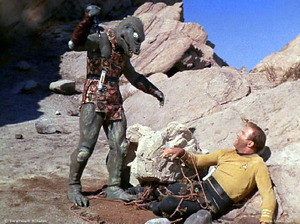
\includegraphics[scale=0.25]{Rationality20From20AI20to20Zombies2020Eliezer20Yudkowsky-img179.jpg}
 \newline
 \textit{Star Trek: The Original Series},
``Arena,'' © CBS Corporation
\par}


\bigskip

{
\ \ \ ~}

{
\ \ \ It's remarkable how the human form is the natural
baseline of the universe, from which all other alien species are
derived via a few modifications.}

{
\ \ \ What could possibly explain this fascinating phenomenon?
Convergent evolution, of course! Even though these alien life-forms
evolved on a thousand alien planets, completely independently from
Earthly life, they all turned out the same.}

{
\ \ \ Don't be fooled by the fact that a kangaroo (a
mammal) resembles us rather less than does a chimp (a primate), nor by
the fact that a frog (amphibians, like us, are tetrapods) resembles us
less than the kangaroo. Don't be fooled by the
bewildering variety of the insects, who split off from us even longer
ago than the frogs; don't be fooled that insects have
six legs, and their skeletons on the outside, and a different system of
optics, and rather different sexual practices.}

{
\ \ \ You might think that a truly alien species would be more different
from us than we are from insects. As I said, don't be
fooled. For an alien species to evolve \textit{intelligence}, it must
have two legs with one knee each attached to an upright torso, and must
walk in a way similar to us. You see, any \textit{intelligence} needs
hands, so you've got to repurpose a pair of legs for
that---and if you don't start with a four-legged being,
it can't develop a running gait and walk upright,
freeing the hands.}

{
\ \ \ .~.~. Or perhaps we should consider, as an alternative theory,
that it's the \textit{easy way out} to use humans in
funny suits.}

{
\ \ \ But the real problem is not shape; it is mind.
``Humans in funny suits'' is a
well-known term in literary science-fiction fandom, and it does
\textit{not} refer to something with four limbs that walks upright. An
angular creature of pure crystal is a ``human in a
funny suit'' if she \textit{thinks} remarkably like a
human---especially a human of an English-speaking culture of the
late-twentieth/early-twenty-first century.}

{
\ \ \ I don't watch a lot of ancient movies. When I was
watching the movie \textit{Psycho} (1960) a few years back, I was taken
aback by the cultural gap between the Americans on the screen and my
America. The buttoned-shirted characters of \textit{Psycho} are
considerably more alien than the vast majority of so-called
``aliens'' I encounter on TV or the
silver screen.}

{
\ \ \ To write a culture that isn't just like your own
culture, you have to be able to see your own culture as a
\textit{special case}{}---not as a norm which all other cultures must
take as their point of departure. Studying history may help---but then
it is only little black letters on little white pages, not a living
experience. I suspect that it would help more to live for a year in
China or Dubai or among the !Kung .~.~. this I have never done, being
busy. Occasionally I wonder what things I might not be seeing (not
there, but here).}

{
\ \ \ Seeing your \textit{humanity} as a special case is very much
harder than this.}

{
\ \ \ In every known culture, humans seem to experience joy, sadness,
fear, disgust, anger, and surprise. In every known culture, these
emotions are indicated by the same facial expressions. Next time you
see an ``alien''---or an
``AI,'' for that matter---I bet that
when it gets angry (and it will get angry), it will show the
human-universal facial expression for anger.}

{
\ \ \ We humans are very much alike under our skulls---that goes with
being a sexually reproducing species; you can't have
everyone using different \textit{complex} adaptations, they
wouldn't assemble. (Do the aliens reproduce sexually,
like humans and many insects? Do they share small bits of genetic
material, like bacteria? Do they form colonies, like fungi? Does the
rule of psychological unity apply among them?)}

{
\ \ \ The only intelligences your ancestors had to
\textit{manipulate}{}---complexly so, and not just tame or catch in
nets---the only minds your ancestors had to model \textit{in
detail}{}---were minds that worked more or less like their own. And so
we evolved to predict Other Minds by putting \textit{ourselves} in
their shoes, asking what we would do in their situations; for that
which was to be predicted, was similar to the predictor.}

{
\ \ \ ``What?'' you say.
``I don't assume other people are just
like me! Maybe I'm sad, and they happen to be angry!
They believe other things than I do; their personalities are different
from mine!'' Look at it this way: a human brain is an
\textit{extremely} complicated physical system. You are not modeling it
neuron-by-neuron or atom-by-atom. If you came across a physical system
as complex as the human brain which was \textit{not} like you, it would
take scientific lifetimes to unravel it. You do \textit{not} understand
how human brains work in an abstract, general sense; you
can't build one, and you can't even
build a computer model that predicts other brains as well as
\textit{you} predict them.}

{
\ \ \ The only reason you can try at all to grasp anything as physically
complex and poorly understood as the brain of another human being is
that you configure your own brain to imitate it. You empathize (though
perhaps not sympathize). You impose on your own brain the shadow of the
other mind's anger and the shadow of its beliefs. You
may never think the words, ``What would I do in this
situation?,'' but that little shadow of the other
mind that you hold within yourself is something animated within your
own brain, invoking the same complex machinery that exists in the other
person, synchronizing gears you don't understand. You
may not be angry yourself, but you know that if \textit{you} were angry
at you, and \textit{you} believed that you were godless scum,
\textit{you} would try to hurt you .~.~.}

{
\ \ \ This ``empathic inference'' (as
I shall call it) works for humans, more or less.}

{
\ \ \ But minds with \textit{different} emotions---minds that feel
emotions you've never felt yourself, or that fail to
feel emotions you would feel? That's something you
can't grasp by putting your brain into the other
brain's shoes. I can tell you to imagine an alien that
grew up in a universe with four spatial dimensions, instead of three
spatial dimensions, but you won't be able to
reconfigure your visual cortex to see like that alien would see. I can
try to write a story about aliens with different emotions, but you
won't be able to feel those emotions, and neither will
I.}

{
\ \ \ Imagine an alien watching a video of the Marx Brothers and having
absolutely no idea what was going on, or why you would actively seek
out such a sensory experience, because the alien has never conceived of
anything remotely like a sense of humor. Don't pity
them for missing out; \textit{you've} never
\textit{antled.}}

{
\ \ \ You might ask: Maybe the aliens do have a sense of humor, but
you're not telling funny enough jokes? This is roughly
the equivalent of trying to speak English very loudly, and very slowly,
in a foreign country, on the theory that those foreigners must have an
inner ghost that can hear the \textit{meaning} dripping from your
words, inherent in your words, if only you can speak them loud enough
to overcome whatever strange barrier stands in the way of your
perfectly sensible English.}

{
\ \ \ It is important to appreciate that laughter can be a beautiful and
valuable thing, even if it is not universalizable, even if it is not
possessed by all possible minds. It would be our own \textit{special}
part of the gift we give to tomorrow. That can count for something
too.}

{
\ \ \ It had better, because universalizability is one metaethical
notion that I can't salvage for you. Universalizability
among humans, maybe; but not among all possible minds.}

{
\ \ \ And what about minds that don't run on emotional
architectures like your own---that don't have things
analogous to \textit{emotions}? No, don't bother
explaining why any intelligent mind powerful enough to build complex
machines must inevitably have states analogous to emotions. Natural
selection builds complex machines without itself having emotions. Now
\textit{there's} a Real Alien for you---an optimization
process that \textit{really} Does Not Work Like You Do.}

{
\ \ \ Much of the progress in biology since the 1960s has consisted of
trying to enforce a moratorium on anthropomorphizing evolution. That
was a major academic slap-fight, and I'm not sure that
sanity would have won the day if not for the availability of crushing
experimental evidence backed up by clear math. Getting people to stop
putting themselves in alien shoes is a long, hard, uphill slog.
I've been fighting that battle on AI for years.}

{
\ \ \ Our anthropomorphism runs very deep in us; it cannot be excised by
a simple act of will, a determination to say, ``Now I
shall stop thinking like a human!'' Humanity is the
air we breathe; it is our \textit{generic}, the white paper on which we
begin our sketches. And we do not think of ourselves as being human
when we are being human.}

{
\ \ \ It is proverbial in literary science fiction that the true test of
an author is their ability to write Real Aliens. (And not just
conveniently incomprehensible aliens who, for their own mysterious
reasons, do whatever the plot happens to require.) Jack Vance was one
of the great masters of this art. Vance's
\textit{humans}, if they come from a different culture, are more alien
than most ``aliens.'' (Never read
any Vance? I would recommend starting with \textit{City of the
Chasch}.) Niven and Pournelle's \textit{The Mote in
God's Eye} also gets a standard mention here.}

{
\ \ \ And conversely---well, I once read a science fiction author (I
think Orson Scott Card) say that the all-time low point of television
science fiction was the \textit{Star Trek} episode where parallel
evolution has proceeded to the extent of producing aliens who not only
look just like humans, who not only speak English, but have also
independently rewritten, word for word, the preamble to the US
Constitution.}

{
\ \ \ This is the Great Failure of Imagination. Don't
think that it's just about science fiction, or even
just about AI. The inability to imagine the alien is the inability to
see \textit{yourself}{}---the inability to understand your own
specialness. Who can see a human camouflaged against a human
background?}

{\centering
\ \ \ \ ~
\par}

{\centering
\ \ \ *
\par}

\mysection{Optimization and the Intelligence Explosion}

{
\ \ \ Among the topics I haven't delved into here is the
notion of an optimization process. Roughly, this is the idea that your
power as a mind is your ability to hit small targets in a large search
space---this can be either the space of possible futures (planning) or
the space of possible designs (invention).}

{
\ \ \ Suppose you have a car, and suppose we already know that your
preferences involve travel. Now suppose that you take all the parts in
the car, or all the atoms, and jumble them up at random.
It's very unlikely that you'll end up
with a travel-artifact at all, even so much as a wheeled cart; let
alone a travel-artifact that ranks as high in your preferences as the
original car. So, relative to your preference ordering, the car is an
extremely \textit{improbable} artifact. The power of an optimization
process is that it can produce this kind of improbability.}

{
\ \ \ You can view both intelligence and natural selection as special
cases of \textit{optimization}: processes that hit, in a large search
space, very small targets defined by implicit preferences. Natural
selection prefers more efficient replicators. Human intelligences have
more complex preferences. Neither evolution nor humans have consistent
utility functions, so viewing them as ``optimization
processes'' is understood to be an approximation.
You're trying to get at the \textit{sort of work being
done}, not claim that humans or evolution do this work
\textit{perfectly}.}

{
\ \ \ This is how I see the story of life and intelligence---as a story
of improbably good designs being produced by optimization processes.
The ``improbability'' here is
improbability relative to a random selection from the design space, not
improbability in an absolute sense---if you have an optimization
process around, then ``improbably''
good designs become probable.}

{
\ \ \ Looking over the history of optimization on Earth up until now,
the first step is to conceptually separate the meta level from the
object level---separate the \textit{structure of optimization} from
\textit{that which is optimized}.}

{
\ \ \ If you consider biology in the absence of hominids, then on the
object level we have things like dinosaurs and butterflies and cats. On
the meta level we have things like sexual recombination and natural
selection of asexual populations. The object level, you will observe,
is rather more complicated than the meta level. Natural selection is
not an \textit{easy} subject and it involves math. But if you look at
the anatomy of a whole cat, the cat has dynamics immensely more
complicated than ``mutate, recombine,
reproduce.''}

{
\ \ \ This is not surprising. Natural selection is an
\textit{accidental} optimization process, that basically just started
happening one day in a tidal pool somewhere. A cat is the
\textit{subject} of millions of years and billions of years of
evolution.}

{
\ \ \ Cats have brains, of course, which operate to learn over a
lifetime; but at the end of the cat's lifetime, that
information is thrown away, so it does not accumulate. The cumulative
effects of cat-brains upon the world as optimizers, therefore, are
relatively small.}

{
\ \ \ Or consider a bee brain, or a beaver brain. A bee builds hives,
and a beaver builds dams; but they didn't figure out
how to build them from scratch. A beaver can't figure
out how to build a hive, a bee can't figure out how to
build a dam.}

{
\ \ \ So animal brains---up until recently---were not major players in
the planetary game of optimization; they were \textit{pieces} but not
\textit{players}. Compared to evolution, brains lacked both generality
of optimization power (they could not produce the amazing range of
artifacts produced by evolution) and cumulative optimization power
(their products did not accumulate complexity over time). For more on
this theme see Protein Reinforcement and DNA Consequentialism.}

{
\ \ \ \textit{Very recently}, certain animal brains have begun to
exhibit both generality of optimization power (producing an amazingly
wide range of artifacts, in time scales too short for natural selection
to play any significant role) and cumulative optimization power
(artifacts of increasing complexity, as a result of skills passed on
through language and writing).}

{
\ \ \ Natural selection takes hundreds of generations to do anything and
millions of years for de novo complex designs. Human programmers can
design a complex machine with a hundred interdependent elements in a
single afternoon. This is not surprising, since natural selection is an
\textit{accidental} optimization process that basically just started
happening one day, whereas humans are \textit{optimized} optimizers
handcrafted by natural selection over millions of years.}

{
\ \ \ The wonder of evolution is not how well it works, but that it
works \textit{at all} without being optimized. This is how optimization
bootstrapped itself into the universe---starting, as one would expect,
from an extremely inefficient accidental optimization process. Which is
not the accidental first replicator, mind you, but the accidental first
process of natural selection. Distinguish the object level and the meta
level!}

{
\ \ \ Since the dawn of optimization in the universe, a certain
structural commonality has held across both natural selection and human
intelligence .~.~.}

{
\ \ \ Natural selection \textit{selects on genes}, but generally
speaking, the genes do not turn around and optimize natural selection.
The invention of sexual recombination is an exception to this rule, and
so is the invention of cells and DNA. And you can see both the power
and the \textit{rarity} of such events, by the fact that evolutionary
biologists structure entire histories of life on Earth around them.}

{
\ \ \ But if you step back and take a human standpoint---if you think
like a programmer---then you can see that natural selection is
\textit{still} not all that complicated. We'll try
bundling different genes together? We'll try separating
information storage from moving machinery? We'll try
randomly recombining groups of genes? On an absolute scale, these are
the sort of bright ideas that any smart hacker comes up with during the
first ten minutes of thinking about system architectures.}

{
\ \ \ Because natural selection started out \textit{so} inefficient (as
a completely accidental process), this tiny handful of meta-level
improvements feeding back in from the replicators---nowhere near as
complicated as the structure of a cat---structure the evolutionary
epochs of life on Earth.}

{
\ \ \ And \textit{after} all that, natural selection is \textit{still} a
blind idiot of a god. Gene pools can evolve to extinction, despite all
cells and sex.}

{
\ \ \ Now natural selection does feed on itself in the sense that each
new adaptation opens up new avenues of further adaptation; but that
takes place on the object level. The gene pool feeds on its own
complexity---but only thanks to the protected interpreter of natural
selection that runs in the background, and that is not itself rewritten
or altered by the evolution of species.}

{
\ \ \ Likewise, human beings invent sciences and technologies, but we
have not \textit{yet} begun to rewrite the protected structure of the
human brain itself. We have a prefrontal cortex and a temporal cortex
and a cerebellum, just like the first inventors of agriculture. We
haven't started to genetically engineer ourselves. On
the object level, science feeds on science, and each new discovery
paves the way for new discoveries---but all that takes place with a
protected interpreter, the human brain, running untouched in the
background.}

{
\ \ \ We have meta-level inventions like science, that try to instruct
humans in how to think. But the first person to invent
Bayes's Theorem did not become a Bayesian; they could
not rewrite themselves, lacking both that knowledge and that power. Our
significant innovations in the art of thinking, like writing and
science, are so powerful that they structure the course of human
history; but they do not rival the brain itself in complexity, and
their effect upon the brain is comparatively shallow.}

{
\ \ \ The present state of the art in rationality training is not
sufficient to turn an arbitrarily selected mortal into Albert Einstein,
which shows the power of a few minor genetic quirks of brain design
compared to all the self-help books ever written in the twentieth
century.}

{
\ \ \ Because the brain hums away invisibly in the background, people
tend to overlook its contribution and take it for granted; and talk as
if the simple instruction to ``Test ideas by
experiment,'' or the p {\textless} 0.05 significance
rule, were the same order of contribution as an entire human brain. Try
telling chimpanzees to test their ideas by experiment and see how far
you get.}

{
\ \ \ Now .~.~. some of us \textit{want} to intelligently design an
intelligence that would be capable of intelligently redesigning itself,
right down to the level of machine code.}

{
\ \ \ The machine code at first, and the laws of physics later, would be
a protected level of a sort. But that ``protected
level'' would not contain the \textit{dynamic of
optimization}; the protected levels would not structure the work. The
human brain does quite a bit of optimization on its own, and screws up
on its own, no matter what you try to tell it in school. But this
\textit{fully wraparound recursive optimizer} would have no protected
level that was \textit{optimizing}. All the structure of optimization
would be subject to optimization itself.}

{
\ \ \ And that is a sea change which breaks with the entire past since
the first replicator, because it breaks the idiom of a protected meta
level.}

{
\ \ \ The history of Earth up until now has been a history of optimizers
spinning their wheels at a constant rate, generating a constant
optimization pressure. And creating optimized products, \textit{not} at
a constant rate, but at an accelerating rate, because of how
object-level innovations open up the pathway to other object-level
innovations. But that acceleration is taking place with a protected
meta level doing the actual optimizing. Like a search that leaps from
island to island in the search space, and good islands tend to be
adjacent to even better islands, but the jumper doesn't
change its legs. \textit{Occasionally}, a few tiny little changes
manage to hit back to the meta level, like sex or science, and then the
history of optimization enters a new epoch and everything proceeds
faster from there.}

{
\ \ \ Imagine an economy without investment, or a university without
language, a technology without tools to make tools. Once in a hundred
million years, or once in a few centuries, someone invents a hammer.}

{
\ \ \ That is what optimization has been like on Earth up until now.}

{
\ \ \ When I look at the history of Earth, I don't see a
history of optimization \textit{over time}. I see a history of
\textit{optimization power} in, and \textit{optimized products} out. Up
until now, thanks to the existence of almost entirely protected
meta-levels, it's been possible to split up the history
of optimization into epochs, and, \textit{within} each epoch, graph the
cumulative \textit{object-level optimization} over time, because the
protected level is running in the background and is not itself changing
within an epoch.}

{
\ \ \ What happens when you build a fully wraparound, recursively
self-improving AI? Then you take the graph of
``optimization in, optimized out,''
and fold the graph in on itself. Metaphorically speaking.}

{
\ \ \ If the AI is weak, it does nothing, because it is not powerful
enough to significantly improve itself---like telling a chimpanzee to
rewrite its own brain.}

{
\ \ \ If the AI is powerful enough to rewrite itself in a way that
increases its ability to make further improvements, and this reaches
all the way down to the AI's full understanding of its
own source code and its own design as an optimizer .~.~. then even if
the graph of ``optimization power
in'' and ``optimized product
out'' looks essentially the same, the graph of
optimization \textit{over time} is going to look completely different
from Earth's history so far.}

{
\ \ \ People often say something like, ``But what if it
requires exponentially greater amounts of self-rewriting for only a
linear improvement?'' To this the obvious answer is,
``Natural selection exerted roughly constant
optimization power on the hominid line in the course of coughing up
humans; and this doesn't seem to have required
exponentially more time for each linear increment of
improvement.''}

{
\ \ \ All of this is still mere analogic reasoning. A full Artificial
General Intelligence thinking about the nature of optimization and
doing its own AI research and rewriting its own source code, is not
\textit{really} like a graph of Earth's history folded
in on itself. It is a different sort of beast. These analogies are
\textit{at best} good for qualitative predictions, and even then, I
have a large amount of other beliefs I haven't yet
explained, which are telling me \textit{which} analogies to make, et
cetera.}

{
\ \ \ But if you want to know why I might be reluctant to extend the
graph of biological and economic growth \textit{over time}, into the
future and over the horizon of an AI that thinks at transistor speeds
and invents self-replicating molecular nanofactories and
\textit{improves its own source code}, then there is my reason: you are
drawing the wrong graph, and it should be optimization power in versus
optimized product out, not optimized product versus time.}

{\centering
\ \ \ \ ~
\par}

{\centering
\ \ \ *
\par}

\mysection{Ghosts in the Machine}

{
\ \ \ People hear about Friendly AI and say---this is one of the top
three initial reactions: }

{
\ \ \ ``Oh, you can try to tell the AI to be Friendly,
but if the AI can modify its own source code, it'll
just remove any constraints you try to place on
it.''}

{
\ \ \ And where does \textit{that} decision come from?}

{
\ \ \ Does it enter from outside causality, rather than being an effect
of a lawful chain of causes that started with the source code as
originally written? Is the AI the ultimate source of its own free
will?}

{
\ \ \ A Friendly AI is not a selfish AI constrained by a special extra
conscience module that overrides the AI's natural
impulses and tells it what to do. You just build the conscience, and
that \textit{is} the AI. If you have a program that computes which
decision the AI should make, you're \textit{done}. The
buck stops immediately.}

{
\ \ \ At this point, I shall take a moment to quote some case studies
from the Computer Stupidities site and Programming subtopic. (I am not
linking to this, because it is a fearsome time-trap; you can Google if
you dare.)}

{
\ \ \ I tutored college students who were taking a computer programming
course. A few of them didn't understand that computers
are not sentient. More than one person used comments in their Pascal
programs to put detailed explanations such as, ``Now I
need you to put these letters on the screen.'' I
asked one of them what the deal was with those comments. The reply:
``How else is the computer going to understand what I
want it to do?'' Apparently they would assume that
since they couldn't make sense of Pascal, neither could
the computer.}

{
\ \ \ While in college, I used to tutor in the school's
math lab. A student came in because his BASIC program would not run. He
was taking a beginner course, and his assignment was to write a program
that would calculate the recipe for oatmeal cookies, depending upon the
number of people you're baking for. I looked at his
program, and it went something like this:}

{
\ \ \ \newline
 10 Preheat oven to 350\newline
 20 Combine all ingredients in a large mixing bowl\newline
 30 Mix until smooth}

{
\ \ \ An introductory programming student once asked me to look at his
program and figure out why it was always churning out zeroes as the
result of a simple computation. I looked at the program, and it was
pretty obvious:}

{
\ \ \ begin\newline
 read({\textquotedbl}Number of Apples{\textquotedbl}, apples)\newline
 read({\textquotedbl}Number of Carrots{\textquotedbl}, carrots)\newline
 read({\textquotedbl}Price for 1 Apple{\textquotedbl}, a\_price)\newline
 read({\textquotedbl}Price for 1 Carrot{\textquotedbl},
c\_price)\newline
 write({\textquotedbl}Total for Apples{\textquotedbl}, a\_total)\newline
 write({\textquotedbl}Total for Carrots{\textquotedbl},
c\_total)\newline
 write({\textquotedbl}Total{\textquotedbl}, total)\newline
 total = a\_total + c\_total\newline
 a\_total = apples * a\_price\newline
 c\_total = carrots * c\_price\newline
 end\newline
}

{
\ \ \ Me: ``Well, your program can't
print correct results before they're
computed.''}

{
\ \ \ Him: ``Huh? It's logical what the
right solution is, and the computer should reorder the instructions the
right way.''}

{
\ \ \ There's an instinctive way of imagining the
scenario of ``programming an AI.''
It maps onto a similar-seeming human endeavor: Telling a human being
what to do. Like the ``program'' is
giving instructions to a little ghost that sits inside the machine,
which will look over your instructions and decide whether it likes them
or not.}

{
\ \ \ There is no ghost who looks over the instructions and decides how
to follow them. The program \textit{is} the AI.}

{
\ \ \ That doesn't mean the ghost does anything you wish
for, like a genie. It doesn't mean the ghost does
everything you want the way you want it, like a slave of exceeding
docility. It means your instruction \textit{is} the only ghost
that's there, at least at boot time.}

{
\ \ \ AI is much harder than people instinctively imagined, exactly
because you can't just \textit{tell} the ghost what to
do. You have to build the ghost from scratch, and everything that seems
obvious to you, the ghost will not see unless you know how to make the
ghost see it. You can't just \textit{tell} the ghost to
see it. You have to create that-which-sees from scratch.}

{
\ \ \ If you don't know how to build something that
seems to have some strange ineffable elements like, say,
``decision-making,'' then you
can't just shrug your shoulders and let the
ghost's free will do the job. You're
left forlorn and ghostless.}

{
\ \ \ There's more to building a chess-playing program
than building a really fast processor---so the AI will be really
smart---and then typing at the command prompt ``Make
whatever chess moves \textit{you} think are best.''
You might think that, since the programmers themselves are not very
good chess players, any advice they tried to give the electronic
superbrain would just slow the ghost down. But there is no ghost. You
see the problem.}

{
\ \ \ And there isn't a simple spell you can perform
to---poof!---summon a complete ghost into the machine. You
can't say, ``I summoned the ghost, and
it appeared; that's cause and effect for
you.'' (It doesn't work if you use
the notion of ``emergence'' or
``complexity'' as a substitute for
``summon,'' either.) You
can't give an instruction to the CPU,
``Be a good chess player!'' You have
to see inside the mystery of chess-playing thoughts, and structure the
whole ghost from scratch.}

{
\ \ \ No matter how common-sensical, no matter how logical, no matter
how ``obvious'' or
``right'' or
``self-evident'' or
``intelligent'' something seems to
you, it will not happen inside the ghost. \textit{Unless} it happens at
the end of a chain of cause and effect that began with the instructions
that \textit{you} had to decide on, plus any causal dependencies on
sensory data that you built into the starting instructions.}

{
\ \ \ This doesn't mean you program in every decision
explicitly. Deep Blue was a chess player far superior to its
programmers. Deep Blue made better chess moves than anything its makers
could have explicitly programmed---but not because the programmers
shrugged and left it up to the ghost. Deep Blue moved better than its
programmers .~.~. at the end of a chain of cause and effect that began
in the programmers' code and proceeded lawfully from
there. Nothing happened \textit{just} because it was so obviously a
good move that Deep Blue's ghostly free will took over,
without the code and its lawful consequences being involved.}

{
\ \ \ If you try to wash your hands of constraining the AI, you
aren't left with a free ghost like an emancipated
slave. You are left with a heap of sand that no one has purified into
silicon, shaped into a CPU and programmed to think.}

{
\ \ \ Go ahead, try telling a computer chip ``Do
whatever you want!'' See what happens? Nothing.
Because you haven't constrained it to understand
freedom.}

{
\ \ \ All it takes is one single step that is \textit{so obvious, so
logical, so self-evident} that your mind just skips right over it, and
you've left the path of the AI programmer. It takes an
effort like the one I illustrate in Grasping Slippery Things to prevent
your mind from doing this.}

{\centering
\ \ \ \ ~
\par}

{\centering
\ \ \ *
\par}

\mysection{Artificial Addition}

{
\ \ \ Suppose that human beings had absolutely \textit{no idea} how they
performed arithmetic. Imagine that human beings had \textit{evolved},
rather than having \textit{learned}, the ability to count sheep and add
sheep. People using this built-in ability have no idea how it worked,
the way Aristotle had no idea how his visual cortex supported his
ability to see things. Peano Arithmetic as we know it has not been
invented. There are philosophers working to formalize numerical
intuitions, but they employ notations such as}

{\centering
\ \ \ Plus-Of(Seven,Six) = Thirteen
\par}


\bigskip

{
\ \ \ to formalize the intuitively obvious fact that when you add
``seven'' plus
``six,'' of course you get
``thirteen.'' }

{
\ \ \ In this world, pocket calculators work by storing a giant lookup
table of arithmetical facts, entered manually by a team of expert
Artificial Arithmeticians, for starting values that range between zero
and one hundred. While these calculators may be helpful in a pragmatic
sense, many philosophers argue that they're only
\textit{simulating} addition, rather than really \textit{adding.} No
machine can really \textit{count}{}---that's why humans
have to count thirteen sheep before typing
``thirteen'' into the calculator.
Calculators can recite back stored facts, but they can never know what
the statements mean---if you type in ``two hundred
plus two hundred'' the calculator says
``Error: Outrange,'' when
it's intuitively \textit{obvious}, if you \textit{know}
what the words \textit{mean}, that the answer is
``four hundred.''}

{
\ \ \ Some philosophers, of course, are not so naive as to be taken in
by these intuitions. Numbers are really a purely formal system---the
label ``thirty-seven'' is
meaningful, not because of any inherent property of the words
themselves, but because the label \textit{refers to} thirty-seven sheep
in the external world. A number is given this referential property by
its \textit{semantic network} of relations to other numbers.
That's why, in computer programs, the LISP token for
``thirty-seven''
doesn't need any \textit{internal}
structure---it's only meaningful because of reference
and relation, not some computational property of
``thirty-seven'' itself.}

{
\ \ \ No one has ever developed an Artificial General Arithmetician,
though of course there are plenty of domain-specific, narrow Artificial
Arithmeticians that work on numbers between
``twenty'' and
``thirty,'' and so on. And if you
look at how slow progress has been on numbers in the range of
``two hundred,'' then it becomes
clear that we're not going to get Artificial General
Arithmetic any time soon. The best experts in the field estimate it
will be at least a hundred years before calculators can add as well as
a human twelve-year-old.}

{
\ \ \ But not everyone agrees with this estimate, or with merely
conventional beliefs about Artificial Arithmetic. It's
common to hear statements such as the following:}

{
\ \ \ ``It's a framing problem---what
`twenty-one plus' equals depends on
whether it's `plus
three' or `plus four.'
If we can just get enough arithmetical facts stored to cover the
common-sense truths that everyone knows, we'll start to
see real addition in the network.''}

{
\ \ \ ``But you'll never be able to
program in that many arithmetical facts by hiring experts to enter them
manually. What we need is an Artificial Arithmetician that can
\textit{learn} the vast network of relations between numbers that
humans acquire during their childhood by observing sets of
apples.''}

{
\ \ \ ``No, what we really need is an Artificial
Arithmetician that can understand natural language, so that instead of
having to be explicitly told that twenty-one plus sixteen equals
thirty-seven, it can get the knowledge by exploring the
Web.''}

{
\ \ \ ``Frankly, it seems to me that
you're just trying to convince yourselves that you can
solve the problem. None of you really know what arithmetic is, so
you're floundering around with these generic sorts of
arguments. `We need an AA that can learn
X,' `We need an AA that can extract X
from the Internet.' I mean, it sounds good, it sounds
like you're making progress, and it's
even good for public relations, because everyone thinks they understand
the proposed solution---but it doesn't really get you
any closer to \textit{general} addition, as opposed to domain-specific
addition. Probably we will never know the fundamental nature of
arithmetic. The problem is just too hard for humans to
solve.''}

{
\ \ \ ``That's why we need to develop a
general arithmetician the same way Nature
did---evolution.''}

{
\ \ \ ``Top-down approaches have clearly failed to
produce arithmetic. We need a bottom-up approach, some way to make
arithmetic \textit{emerge.} We have to acknowledge the basic
unpredictability of complex systems.''}

{
\ \ \ ``You're all wrong. Past efforts
to create machine arithmetic were futile from the start, because they
just didn't have enough computing power. If you look at
how many trillions of synapses there are in the human brain,
it's clear that calculators don't have
lookup tables anywhere near that large. We need calculators as powerful
as a human brain. According to Moore's Law, this will
occur in the year 2031 on April 27 between 4:00 and 4:30 in the
morning.''}

{
\ \ \ ``I believe that machine arithmetic will be
developed when researchers scan each neuron of a complete human brain
into a computer, so that we can simulate the biological circuitry that
performs addition in humans.''}

{
\ \ \ ``I don't think we have to wait
to scan a whole brain. Neural networks are just like the human brain,
and you can train them to do things without knowing how they do them.
We'll create programs that will do arithmetic without
we, our creators, ever understanding how they do
arithmetic.''}

{
\ \ \ ``But Gödel's Theorem shows that
no formal system can ever capture the basic properties of arithmetic.
Classical physics is formalizable, so to add two and two, the brain
must take advantage of quantum physics.''}

{
\ \ \ ``Hey, if human arithmetic were simple enough
that we could reproduce it in a computer, we wouldn't
be able to count high enough to build computers.''}

{
\ \ \ ``Haven't you heard of John
Searle's Chinese Calculator Experiment? Even if you did
have a huge set of rules that would let you add
`twenty-one' and
`sixteen,' just imagine translating all
the words into Chinese, and you can see that there's no
genuine addition going on. There are no real \textit{numbers} anywhere
in the system, just labels that humans use for numbers
.~.~.''}

{
\ \ \ There is more than one moral to this parable, and I have told it
with different morals in different contexts. It illustrates the idea of
levels of organization, for example---a CPU can add two large numbers
because the numbers aren't black-box opaque objects,
they're ordered structures of 32 bits.}

{
\ \ \ But for purposes of overcoming bias, let us draw two morals:}

{
\ \ \ First, the danger of believing assertions you
can't regenerate from your own knowledge.}

{
\ \ \ Second, the danger of trying to dance around basic confusions.}

{
\ \ \ Lest anyone accuse me of generalizing from fictional evidence,
both lessons may be drawn from the real history of Artificial
Intelligence as well.}

{
\ \ \ The first danger is the object-level problem that the AA devices
ran into: they functioned as tape recorders playing back
``knowledge'' generated from outside
the system, using a process they couldn't capture
internally. A human could tell the AA device that
``twenty-one plus sixteen equals
thirty-seven,'' and the AA devices could record this
sentence and play it back, or even pattern-match
``twenty-one plus sixteen'' to
output ``thirty-seven!''---but the
AA devices couldn't generate such knowledge for
themselves.}

{
\ \ \ Which is strongly reminiscent of believing a physicist who tells
you ``Light is waves,'' recording
the fascinating words and playing them back when someone asks
``What is light made of?,'' without
being able to generate the knowledge for yourself.}

{
\ \ \ The second moral is the meta-level danger that consumed the
Artificial Arithmetic researchers and opinionated bystanders---the
danger of dancing around confusing gaps in your knowledge. The tendency
to do just about anything \textit{except} grit your teeth and buckle
down and fill in the damn gap.}

{
\ \ \ Whether you say, ``It is
emergent!,'' or whether you say,
``It is unknowable!,'' in neither
case are you acknowledging that there is a basic insight required which
is possessable, but unpossessed by you.}

{
\ \ \ How can you know when you'll have a new basic
insight? And there's no way to get one except by
banging your head against the problem, learning everything you can
about it, studying it from as many angles as possible, perhaps for
years. It's not a pursuit that academia is set up to
permit, when you need to publish at least one paper per month.
It's certainly not something that venture capitalists
will fund. You want to either go ahead and build the system
\textit{now}, or give up and do something else instead.}

{
\ \ \ Look at the comments above: none are aimed at setting out on a
quest for the missing insight which would \textit{make numbers no
longer mysterious}, make
``twenty-seven'' more than a black
box. None of the commenters realized that their difficulties arose from
ignorance or confusion in their own minds, rather than an inherent
property of arithmetic. They were not trying to achieve a state where
the confusing thing ceased to be confusing.}

{
\ \ \ If you read Judea Pearl's \textit{Probabilistic
Reasoning in Intelligent Systems: Networks of Plausible
Inference},\textsuperscript{1} then you will see that the basic insight
behind graphical models is \textit{indispensable} to problems that
require it. (It's not something that fits on a T-shirt,
I'm afraid, so you'll have to go and
read the book yourself. I haven't seen any online
popularizations of Bayesian networks that adequately convey the reasons
behind the principles, or the importance of the math being exactly the
way it is, but Pearl's book is wonderful.) There were
once dozens of ``non-monotonic
logics'' awkwardly trying to capture intuitions such
as ``If my burglar alarm goes off, there was probably
a burglar, but if I then learn that there was a small earthquake near
my home, there was probably not a burglar.'' With the
graphical-model insight in hand, you can give a mathematical
explanation of exactly why first-order logic has the wrong properties
for the job, and express the correct solution in a compact way that
captures all the common-sense details in one elegant swoop. Until you
have that insight, you'll go on patching the logic
here, patching it there, adding more and more hacks to force it into
correspondence with everything that seems ``obviously
true.''}

{
\ \ \ You won't \textit{know} the Artificial Arithmetic
problem is unsolvable without its key. If you don't
know the rules, you don't know the rule that says you
need to know the rules to do anything. And so there will be all sorts
of clever ideas that seem like they might work, like building an
Artificial Arithmetician that can read natural language and download
millions of arithmetical assertions from the Internet.}

{
\ \ \ And yet \textit{somehow} the clever ideas never work. Somehow it
always turns out that you ``couldn't
see any reason it wouldn't work''
because you were ignorant of the obstacles, not because no obstacles
existed. Like shooting blindfolded at a distant target---you can fire
blind shot after blind shot, crying, ``You
can't prove to me that I won't hit the
center!'' But until you take off the blindfold,
you're not even in the aiming game. When
``no one can prove to you'' that
your precious idea \textit{isn't} right, it means you
don't have enough information to strike a small target
in a vast answer space. \textit{Until you know your idea will work, it
won't.}}

{
\ \ \ From the history of previous key insights in Artificial
Intelligence, and the grand messes that were proposed prior to those
insights, I derive an important real-life lesson: \textit{When the
basic problem is your ignorance, clever strategies for bypassing your
ignorance lead to shooting yourself in the foot.}}

{\centering
\ \ \ \ ~
\par}

{\centering
\ \ \ *
\par}


\bigskip

{
\ \ \ 1. Pearl, \textit{Probabilistic Reasoning in Intelligent
Systems}.}

\mysection{Terminal Values and Instrumental Values}

{
\ \ \ On a purely instinctive level, any human planner behaves as if
they distinguish between means and ends. Want chocolate?
There's chocolate at the Publix supermarket. You can
get to the supermarket if you drive one mile south on Washington Ave.
You can drive if you get into the car. You can get into the car if you
open the door. You can open the door if you have your car keys. So you
put your car keys into your pocket, and get ready to leave the house
.~.~. }

{
\ \ \ .~.~. when suddenly the word comes on the radio that an earthquake
has destroyed all the chocolate at the local Publix. Well,
there's no point in driving to the Publix if
there's no chocolate there, and no point in getting
into the car if you're not driving anywhere, and no
point in having car keys in your pocket if you're not
driving. So you take the car keys out of your pocket, and call the
local pizza service and have them deliver a chocolate pizza. Mm,
delicious.}

{
\ \ \ I rarely notice people losing track of plans they devised
themselves. People usually don't drive to the
supermarket if they know the chocolate is gone. But
I've also noticed that when people begin
\textit{explicitly} talking about goal systems instead of just
\textit{wanting} things, \textit{mentioning}
``goals'' instead of \textit{using}
them, they oft become confused. Humans are experts at planning, not
experts on planning, or there'd be a lot more AI
developers in the world.}

{
\ \ \ In particular, I've noticed people get confused
when---in abstract philosophical discussions rather than everyday
life---they consider the distinction between means and ends; more
formally, between ``instrumental
values'' and ``terminal
values.''}

{
\ \ \ Part of the problem, it seems to me, is that the human mind uses a
rather ad-hoc system to keep track of its goals---it works, but not
cleanly. English doesn't embody a sharp distinction
between means and ends: ``I want to save my
sister's life'' and
``I want to administer penicillin to my
sister'' use the same word
``want.''}

{
\ \ \ Can we describe, in mere English, the distinction that is getting
lost?}

{
\ \ \ As a first stab:}

{
\ \ \ ``Instrumental values'' are
desirable strictly conditional on their anticipated consequences.
``I want to administer penicillin to my
sister,'' not because a penicillin-filled sister is
an intrinsic good, but in anticipation of penicillin curing her
flesh-eating pneumonia. If instead you anticipated that injecting
penicillin would melt your sister into a puddle like the Wicked Witch
of the West, you'd fight just as hard to keep her
penicillin-free.}

{
\ \ \ ``Terminal values'' are
desirable without conditioning on other consequences:
``I want to save my sister's
life'' has nothing to do with your anticipating
whether she'll get injected with penicillin after
that.}

{
\ \ \ This first attempt suffers from obvious flaws. If saving my
sister's life would cause the Earth to be swallowed up
by a black hole, then I would go off and cry for a while, but I
wouldn't administer penicillin. Does this mean that
saving my sister's life was not a
``terminal'' or
``intrinsic'' value, because
it's theoretically conditional on its consequences? Am
I \textit{only} trying to save her life because of my belief that a
black hole won't consume the Earth afterward? Common
sense should say that's not what's
happening.}

{
\ \ \ So forget English. We can set up a mathematical description of a
decision system in which terminal values and instrumental values are
separate and incompatible types---like integers and floating-point
numbers, in a programming language with no automatic conversion between
them.}

{
\ \ \ An ideal Bayesian decision system can be set up using only four
elements:}

{
\ \ \  Outcomes : type Outcome[] list of possible outcomes
{\textbackslash}{\textquotesingle}7bsister lives, sister
dies{\textbackslash}{\textquotesingle}7d }

{
\ \ \  Actions : type Action[] list of possible actions
{\textbackslash}{\textquotesingle}7badminister penicillin,
don't administer
penicillin{\textbackslash}{\textquotesingle}7d }

{
\ \ \  Utility\_function : type Outcome -{\textgreater} Utility utility
function that maps each outcome onto a utility (a utility being
representable as a real number between negative and positive infinity)
{\textbackslash}{\textquotesingle}7bsister lives $\rightarrow $ 1,
sister dies $\rightarrow $ 0{\textbackslash}{\textquotesingle}7d }

{
\ \ \  Conditional\_probability\_function :\newline
 type Action -{\textgreater} (Outcome -{\textgreater} Probability)
conditional probability function that maps each action onto a
probability distribution over outcomes (a probability being
representable as a real number between 0 and 1)
{\textbackslash}{\textquotesingle}7badminister penicillin $\rightarrow
$ (sister lives $\rightarrow $ 0.9, sister dies $\rightarrow $ 0.1),
don't administer penicillin $\rightarrow $ (sister
lives $\rightarrow $ 0.3, sister dies $\rightarrow $
0.7){\textbackslash}{\textquotesingle}7d }

{
\ \ \ If you can't read the type system directly,
don't worry, I'll always translate into
English. For programmers, seeing it described in distinct statements
helps to set up distinct mental objects.}

{
\ \ \ And the decision system itself?}

{
\ \ \  Expected\_Utility : Action A -{\textgreater}\newline
 (Sum O in Outcomes: Utility(O) * Probability(O{\textbar}A)) The
``expected utility'' of an action
equals the sum, over all outcomes, of the utility of that outcome times
the conditional probability of that outcome given that action.
{\textbackslash}{\textquotesingle}7bEU(administer penicillin) = 0.9,
EU(don't administer penicillin) =
0.3{\textbackslash}{\textquotesingle}7d }

{
\ \ \  Choose :\newline
 -{\textgreater} (Argmax A in Actions: Expected\_Utility(A)) Pick an
action whose ``expected utility'' is
maximal. {\textbackslash}{\textquotesingle}7breturn: administer
penicillin{\textbackslash}{\textquotesingle}7d }

{
\ \ \ For every action, calculate the conditional probability of all the
consequences that might follow, then add up the utilities of those
consequences times their conditional probability. Then pick the best
action.}

{
\ \ \ This is a mathematically simple sketch of a decision system. It is
not an efficient way to compute decisions in the real world.}

{
\ \ \ What if, for example, you need a \textit{sequence} of acts to
carry out a plan? The formalism can easily represent this by letting
each Action stand for a whole sequence. But this creates an
exponentially large space, like the space of all sentences you can type
in 100 letters. As a simple example, if one of the possible acts on the
first turn is ``Shoot my own foot
off,'' a human planner will decide this is a bad idea
generally---eliminate \textit{all} sequences beginning with this
action. But we've flattened this structure out of our
representation. We don't have sequences of acts, just
flat ``actions.''}

{
\ \ \ So, yes, there are \textit{a few minor complications.} Obviously
so, or we'd just run out and build a real AI this way.
In that sense, it's much the same as Bayesian
probability theory itself.}

{
\ \ \ But this is one of those times when it's a
\textit{surprisingly good idea} to consider the absurdly simple version
before adding in any high-falutin' complications.}

{
\ \ \ Consider the philosopher who asserts, ``All of us
are ultimately selfish; we care only about our own states of mind. The
mother who claims to care about her son's welfare,
really wants to \textit{believe} that her son is doing well---this
belief is what makes the mother happy. She helps him for the sake of
her own happiness, not his.'' You say,
``Well, suppose the mother sacrifices her life to push
her son out of the path of an oncoming truck. That's
not going to make her happy, just dead.'' The
philosopher stammers for a few moments, then replies,
``But she still did it because \textit{she valued}
that choice above others---because of the \textit{feeling of
importance} she attached to that decision.''}

{
\ \ \ So you say,}

{
\ \ \ TYPE ERROR: No constructor found for Expected\_Utility
-{\textgreater} Utility.}

{
\ \ \ Allow me to explain that reply.}

{
\ \ \ Even our simple formalism illustrates a sharp distinction between
\textit{expected utility}, which is something that \textit{actions}
have; and \textit{utility}, which is something that \textit{outcomes}
have. Sure, you can map both utilities and expected utilities onto real
numbers. But that's like observing that you can map
wind speed and temperature onto real numbers. It
doesn't make them the same thing.}

{
\ \ \ The philosopher begins by arguing that all your Utilities must be
over Outcomes consisting of your state of mind. If this were true, your
intelligence would operate \textit{as an engine to steer the future}
into regions where you were happy. Future states would be distinguished
only by your state of mind; you would be indifferent between any two
futures in which you had the same state of mind.}

{
\ \ \ And you would, indeed, be rather unlikely to sacrifice your own
life to save another.}

{
\ \ \ When we object that people sometimes \textit{do} sacrifice their
lives, the philosopher's reply shifts to discussing
Expected Utilities over Actions: ``The feeling of
\textit{importance} she attached to that
\textit{decision}.'' This is a drastic jump that
\textit{should} make us leap out of our chairs in indignation. Trying
to convert an Expected\_Utility into a Utility would cause an outright
error in our programming language. But in English it all sounds the
same.}

{
\ \ \ The choices of our simple decision system are those with highest
Expected\_Utility, but this doesn't say anything
whatsoever about \textit{where it steers the future.} It
doesn't say anything about the utilities the decider
assigns, or which real-world outcomes are likely to happen as a result.
It doesn't say anything about the
mind's function as an engine.}

{
\ \ \ The physical cause of a physical action is a cognitive state, in
our ideal decider an Expected\_Utility, and this expected utility is
calculated by evaluating a utility function over imagined consequences.
To save your son's life, you must imagine the event of
your son's life being saved, and this imagination is
not the event itself. It's a \textit{quotation}, like
the difference between ``snow'' and
snow. But that doesn't mean that what's
\textit{inside the quote marks} must itself be a cognitive state. If
you choose the action that leads to the future that you represent with
``my son is still alive,'' then you
have functioned as an engine to steer the future into a region where
your son is still alive. Not an engine that steers the future into a
region where \textit{you represent the sentence} ``my
son is still alive.'' To steer the future
\textit{there}, your utility function would have to return a high
utility when fed ````my son is still
alive'''', the quotation of the
quotation, your imagination of yourself imagining. Recipes make poor
cake when you grind them up and toss them in the batter.}

{
\ \ \ And that's why it's helpful to
consider the simple decision systems first. Mix enough complications
into the system, and formerly clear distinctions become harder to see.}

{
\ \ \ So now let's look at some complications. Clearly
the Utility function (mapping Outcomes onto Utilities) is meant to
formalize what I earlier referred to as ``terminal
values,'' values not contingent upon their
consequences. What about the case where saving your
sister's life leads to Earth's
destruction by a black hole? In our formalism, we've
flattened out this possibility. Outcomes don't lead to
Outcomes, only Actions lead to Outcomes. Your sister recovering from
pneumonia \textit{followed by} the Earth being devoured by a black hole
would be flattened into a single ``possible
outcome.''}

{
\ \ \ And where are the ``instrumental
values'' in this simple formalism? Actually,
they've vanished entirely! You see, in this formalism,
actions lead directly to outcomes with no intervening events.
There's no notion of throwing a rock that flies through
the air and knocks an apple off a branch so that it falls to the
ground. Throwing the rock is the Action, and it leads straight to the
Outcome of the apple lying on the ground---according to the conditional
probability function that turns an Action directly into a Probability
distribution over Outcomes.}

{
\ \ \ In order to \textit{actually compute} the conditional probability
function, and in order to separately consider the utility of a
sister's pneumonia and a black hole swallowing Earth,
we would have to represent the network structure of causality---the way
that events lead to other events.}

{
\ \ \ And then the instrumental values would start coming back. If the
causal network was sufficiently regular, you could find a state B that
tended to lead to C regardless of how you achieved B. Then if you
wanted to achieve C for some reason, you could plan efficiently by
first working out a B that led to C, and then an A that led to B. This
would be the phenomenon of ``instrumental
value''---B would have
``instrumental value'' because it
led to C. The state C itself might be terminally valued---a term in the
utility function over the total outcome. Or C might just be an
instrumental value, a node that was not directly valued by the utility
function.}

{
\ \ \ Instrumental value, in this formalism, is purely an aid to the
efficient computation of plans. It can and should be discarded wherever
this kind of regularity does not exist.}

{
\ \ \ Suppose, for example, that there's some particular
value of B that doesn't lead to C. Would you choose an
A which led to that B? Or never mind the abstract philosophy: If you
wanted to go to the supermarket to get chocolate, and you wanted to
drive to the supermarket, and you needed to get into your car, would
you gain entry by ripping off the car door with a steam shovel? (No.)
Instrumental value is a ``leaky
abstraction,'' as we programmers say; you sometimes
have to toss away the cached value and compute out the actual expected
utility. Part of being \textit{efficient} without being
\textit{suicidal} is noticing when convenient shortcuts break down.
Though this formalism does give rise to instrumental values, it does so
only where the requisite regularity exists, and strictly as a
convenient shortcut in computation.}

{
\ \ \ But if you complicate the formalism before you understand the
simple version, then you may start thinking that instrumental values
have some strange life of their own, even in a normative sense. That,
once you say B is usually good because it leads to C,
you've committed yourself to always try for B even in
the absence of C. People make this kind of mistake in abstract
philosophy, even though they would never, in real life, rip open their
car door with a steam shovel. You may start thinking that
there's no way to develop a consequentialist that
maximizes only inclusive genetic fitness, because it will starve unless
you include an explicit terminal value for ``eating
food.'' People make this mistake even though they
would never stand around opening car doors all day long, for fear of
being stuck outside their cars if they didn't have a
terminal value for opening car doors.}

{
\ \ \ Instrumental values live in (the network structure of) the
conditional probability function. This makes instrumental value
strictly dependent on beliefs-of-fact given a fixed utility function.
If I believe that penicillin causes pneumonia, and that the absence of
penicillin cures pneumonia, then my perceived instrumental value of
penicillin will go from high to low. Change the beliefs of
fact---change the conditional probability function that associates
actions to believed consequences---and the instrumental values will
change in unison.}

{
\ \ \ In moral arguments, some disputes are about instrumental
consequences, and some disputes are about terminal values. If your
debating opponent says that banning guns will lead to lower crime, and
you say that banning guns will lead to higher crime, then you agree
about a superior instrumental value (crime is bad), but you disagree
about which intermediate events lead to which consequences. But I do
not think an argument about female circumcision is really a factual
argument about how to best achieve a shared value of treating women
fairly or making them happy.}

{
\ \ \ This important distinction often gets \textit{flushed down the
toilet} in angry arguments. People with factual disagreements and
shared values each decide that their debating opponents must be
sociopaths. As if your hated enemy, gun control/rights advocates,
\textit{really wanted to kill people}, which should be implausible as
realistic psychology.}

{
\ \ \ I fear the human brain does not strongly type the distinction
between terminal moral beliefs and instrumental moral beliefs.
``We should ban guns'' and
``We should save lives''
don't \textit{feel different}, as moral beliefs, the
way that sight feels different from sound. Despite all the other ways
that the human goal system complicates everything in sight, this
\textit{one distinction} it manages to collapse into a mishmash of
things-with-conditional-value.}

{
\ \ \ To extract out the terminal values we have to inspect this
mishmash of valuable things, trying to figure out which ones are
getting their value from somewhere else. It's a
difficult project! If you say that you want to ban guns in order to
reduce crime, it may take a moment to realize that
``reducing crime''
isn't a terminal value, it's a superior
instrumental value with links to terminal values for human lives and
human happinesses. And then the one who advocates gun rights may have
links to the superior instrumental value of ``reducing
crime'' plus a link to a value for
``freedom,'' which might be a
terminal value unto them, or another instrumental value .~.~.}

{
\ \ \ We can't print out our complete network of values
derived from other values. We probably don't even store
the whole history of how values got there. By considering the right
moral dilemmas, ``Would you do X if
Y,'' we can often figure out where our values came
from. But even this project itself is full of pitfalls; misleading
dilemmas and gappy philosophical arguments. We don't
know what our own values are, or where they came from, and
can't find out except by undertaking error-prone
projects of cognitive archaeology. Just forming a conscious distinction
between ``terminal value'' and
``instrumental value,'' and keeping
track of what it means, and using it correctly, is hard work. Only by
inspecting the simple formalism can we see how easy it ought to be, in
principle.}

{
\ \ \ And that's to say nothing of all the other
complications of the human reward system---the whole use of
reinforcement architecture, and the way that eating chocolate is
pleasurable, and anticipating eating chocolate is pleasurable, but
they're different kinds of pleasures .~.~.}

{
\ \ \ But I don't complain too much about the mess.}

{
\ \ \ Being ignorant of your own values may not always be fun, but at
least it's not boring.}

{\centering
\ \ \ \ ~
\par}

{\centering
\ \ \ *
\par}

\mysection{Leaky Generalizations}

{
\ \ \ Are apples good to eat? Usually, but some apples are rotten. }

{
\ \ \ Do humans have ten fingers? Most of us do, but plenty of people
have lost a finger and nonetheless qualify as
``human.''}

{
\ \ \ Unless you descend to a level of description far below any
macroscopic object---below societies, below people, below fingers,
below tendon and bone, below cells, all the way down to particles and
fields where the laws are truly universal---practically every
generalization you use in the real world will be leaky.}

{
\ \ \ (Though there may, of course, be some exceptions to the above rule
.~.~.)}

{
\ \ \ Mostly, the way you deal with leaky generalizations is that, well,
you just have to deal. If the cookie market almost always closes at 10
p.m., except on Thanksgiving it closes at 6 p.m., and today happens to
be National Native American Genocide Day, you'd better
show up before 6 p.m. or you won't get a cookie.}

{
\ \ \ Our ability to manipulate leaky generalizations is opposed by
\textit{need for closure}, the degree to which we want to say once and
for all that humans have ten fingers, and get frustrated when we have
to tolerate continued ambiguity. Raising the value of the stakes can
increase need for closure---which shuts down complexity tolerance when
complexity tolerance is most needed.}

{
\ \ \ Life would be complicated even if the things we wanted were simple
(they aren't). The leakyness of leaky generalizations
about what-to-do-next would leak in from the leaky structure of the
real world. Or to put it another way:}

{
\ \ \ Instrumental values often have no specification that is both
compact and local.}

{
\ \ \ Suppose there's a box containing a million
dollars. The box is locked, not with an ordinary combination lock, but
with a dozen keys controlling a machine that can open the box. If you
know how the machine works, you can deduce which sequences of
key-presses will open the box. There's more than one
key sequence that can trigger the machine to open the box. But if you
press a sufficiently wrong sequence, the machine incinerates the money.
And if you \textit{don't know} about the machine,
there's no simple rules like
``Pressing any key three times opens the
box'' or ``Pressing five different
keys with no repetitions incinerates the money.''}

{
\ \ \ There's a \textit{compact nonlocal} specification
of which keys you want to press: You want to press keys such that they
open the box. You can write a compact computer program that computes
which key sequences are good, bad or neutral, but the computer program
will need to describe the machine, not just the keys themselves.}

{
\ \ \ There's likewise a \textit{local noncompact}
specification of which keys to press: a giant lookup table of the
results for each possible key sequence. It's a very
large computer program, but it makes no mention of anything except the
keys.}

{
\ \ \ But there's no way to describe which key sequences
are good, bad, or neutral, which is both \textit{simple} and phrased
\textit{only in terms of the keys themselves.}}

{
\ \ \ It may be even worse if there are tempting local generalizations
which turn out to be \textit{leaky}. Pressing \textit{most} keys three
times in a row will open the box, but there's a
particular key that incinerates the money if you press it just once.
You might think you had found a perfect generalization---a locally
describable class of sequences that \textit{always} opened the
box---when you had merely failed to visualize all the possible paths of
the machine, or failed to value all the side effects.}

{
\ \ \ The machine represents the complexity of the real world. The
openness of the box (which is good) and the incinerator (which is bad)
represent the thousand shards of desire that make up our terminal
values. The keys represent the actions and policies and strategies
available to us.}

{
\ \ \ When you consider how many different ways we value outcomes, and
how complicated are the paths we take to get there,
it's a wonder that there exists any such thing as
helpful ethical \textit{advice}. (Of which the strangest of all
advices, \textit{and yet still helpful}, is that ``the
end does not justify the means.'')}

{
\ \ \ But conversely, the complicatedness of action need not say
anything about the complexity of goals. You often find people who smile
wisely, and say, ``Well, morality is complicated, you
know, female circumcision is right in one culture and wrong in another,
it's not always a bad thing to torture people. How
naive you are, how full of need for closure, that you think there are
any simple rules.''}

{
\ \ \ You can say, unconditionally and flatly, that killing
\textit{anyone} is a huge dose of negative terminal utility. Yes, even
Hitler. That doesn't mean you shouldn't
shoot Hitler. It means that the net instrumental utility of shooting
Hitler carries a giant dose of negative utility from
Hitler's death, and a hugely larger dose of positive
utility from all the other lives that would be saved as a consequence.}

{
\ \ \ Many commit the type error that I warned against in Terminal
Values and Instrumental Values, and think that if the net consequential
expected utility of Hitler's death is conceded to be
positive, then the immediate local terminal utility must also be
positive, meaning that the moral principle ``Death is
always a bad thing'' is itself a leaky
generalization. But this is double counting, with utilities instead of
probabilities; you're setting up a resonance between
the expected utility and the utility, instead of a one-way flow from
utility to expected utility.}

{
\ \ \ Or maybe it's just the urge toward a one-sided
policy debate: the best policy must have \textit{no} drawbacks.}

{
\ \ \ In my moral philosophy, the \textit{local} negative utility of
Hitler's death is stable, no matter what happens to the
external consequences and hence to the \textit{expected} utility.}

{
\ \ \ Of course, you can set up a moral argument that
it's an \textit{inherently} good thing to punish evil
people, even with capital punishment for sufficiently evil people. But
you can't carry this moral argument by pointing out
that the \textit{consequence} of shooting a man holding a leveled gun
may be to save other lives. This is appealing to the value of life, not
appealing to the value of death. If expected utilities are leaky and
complicated, it doesn't mean that utilities must be
leaky and complicated as well. They might be! But it would be a
separate argument.}

{\centering
\ \ \ \ ~
\par}

{\centering
\ \ \ *
\par}

\mysection{The Hidden Complexity of Wishes}

{
\ \ \ I wish to live in the locations of my choice, in a physically
healthy, uninjured, and apparently normal version of my current body
containing my current mental state, a body which will heal from all
injuries at a rate three sigmas faster than the average given the
medical technology available to me, and which will be protected from
any diseases, injuries or illnesses causing disability, pain, or
degraded functionality or any sense, organ, or bodily function for more
than ten days consecutively or fifteen days in any year .~.~.}

{\raggedleft
\ \ \ {}---The Open-Source Wish Project, Wish For Immortality 1.1
\par}


\bigskip

{
\ \ \ ~}

{
\ \ \ There are three kinds of genies: Genies to whom you can safely
say, ``I wish for you to do what I should wish
for''; genies for which \textit{no} wish is safe; and
genies that aren't very powerful or intelligent.}

{
\ \ \ Suppose your aged mother is trapped in a burning building, and it
so happens that you're in a wheelchair; you
can't rush in yourself. You could cry,
``Get my mother out of that
building!'' but there would be no one to hear.}

{
\ \ \ Luckily you have, in your pocket, an Outcome Pump. This handy
device squeezes the flow of time, pouring probability into some
outcomes, draining it from others.}

{
\ \ \ The Outcome Pump is not sentient. It contains a tiny time machine,
which resets time \textit{unless} a specified outcome occurs. For
example, if you hooked up the Outcome Pump's sensors to
a coin, and specified that the time machine should keep resetting until
it sees the coin come up heads, and then you actually flipped the coin,
\textit{you} would see the coin come up heads. (The physicists say that
any future in which a ``reset''
occurs is inconsistent, and therefore never happens in the first
place---so you aren't actually killing any versions of
yourself.)}

{
\ \ \ Whatever proposition you can manage to input into the Outcome Pump
\textit{somehow happens}, though not in a way that violates the laws of
physics. If you try to input a proposition that's
\textit{too} unlikely, the time machine will suffer a spontaneous
mechanical failure before that outcome ever occurs.}

{
\ \ \ You can also redirect probability flow in more quantitative ways,
using the ``future function'' to
scale the temporal reset probability for different outcomes. If the
temporal reset probability is 99\% when the coin comes up heads, and
1\% when the coin comes up tails, the odds will go from 1:1 to 99:1 in
favor of tails. If you had a mysterious machine that spit out money,
and you wanted to maximize the amount of money spit out, you would use
reset probabilities that diminished as the amount of money increased.
For example, spitting out \$10 might have a 99.999999\% reset
probability, and spitting out \$100 might have a 99.99999\% reset
probability. This way you can get an outcome that tends to be as high
as possible in the future function, even when you don't
know the best attainable maximum.}

{
\ \ \ So you desperately yank the Outcome Pump from your pocket---your
mother is still trapped in the burning building, remember?---and try to
describe your goal: \textit{get your mother out of the building!}}

{
\ \ \ The user interface doesn't take English inputs.
The Outcome Pump isn't sentient, remember? But it does
have 3D scanners for the near vicinity, and built-in utilities for
pattern matching. So you hold up a photo of your
mother's head and shoulders; match on the photo; use
object contiguity to select your mother's whole body
(not just her head and shoulders); and define the \textit{future
function} using your mother's distance from the
building's center. The further she gets from the
building's center, the less the time
machine's reset probability.}

{
\ \ \ You cry ``Get my mother out of the
building!,'' for luck, and press Enter.}

{
\ \ \ For a moment it seems like nothing happens. You look around,
waiting for the fire truck to pull up, and rescuers to arrive---or even
just a strong, fast runner to haul your mother out of the building---}

{
\ \ \ \textit{BOOM!} With a thundering roar, the gas main under the
building explodes. As the structure comes apart, in what seems like
slow motion, you glimpse your mother's shattered body
being hurled high into the air, traveling fast, rapidly increasing its
distance from the former center of the building.}

{
\ \ \ On the side of the Outcome Pump is an Emergency Regret Button. All
future functions are automatically defined with a huge negative value
for the Regret Button being pressed---a temporal reset probability of
nearly 1---so that the Outcome Pump is extremely unlikely to do
anything which upsets the user enough to make them press the Regret
Button. You can't ever remember pressing it. But
you've barely started to reach for the Regret Button
(and what good will it do now?) when a flaming wooden beam drops out of
the sky and smashes you flat.}

{
\ \ \ Which wasn't really what you wanted, but scores
very high in the defined future function .~.~.}

{
\ \ \ The Outcome Pump is a genie of the second class. \textit{No} wish
is safe.}

{
\ \ \ If someone asked you to get their poor aged mother out of a
burning building, you might help, or you might pretend not to hear. But
it wouldn't even \textit{occur} to you to explode the
building. ``Get my mother out of the
building'' \textit{sounds} like a much safer wish
than it really is, because you don't even
\textit{consider} the plans that you assign extreme negative values.}

{
\ \ \ Consider again the Tragedy of Group Selectionism: Some early
biologists asserted that group selection for low subpopulation sizes
would produce individual restraint in breeding; and yet actually
enforcing group selection in the laboratory produced cannibalism,
especially of immature females. It's obvious in
hindsight that, given strong selection for small subpopulation sizes,
cannibals will outreproduce individuals who voluntarily forego
reproductive opportunities. But eating little girls is such an
\textit{un-aesthetic} solution that Wynne-Edwards, Allee, Brereton, and
the other group-selectionists simply didn't think of
it. They only saw the solutions they would have used themselves.}

{
\ \ \ Suppose you try to patch the future function by specifying that
the Outcome Pump should not explode the building: outcomes in which the
building materials are distributed over too much volume will have \~{}1
temporal reset probabilities.}

{
\ \ \ So your mother falls out of a second-story window and breaks her
neck. The Outcome Pump took a different path through time that still
ended up with your mother outside the building, and it still
wasn't what you wanted, and it still
wasn't a solution that would occur to a human rescuer.}

{
\ \ \ If only the Open-Source Wish Project had developed a Wish To Get
Your Mother Out Of A Burning Building:}

{
\ \ \ I wish to move my mother (defined as the woman who shares half my
genes and gave birth to me) to outside the boundaries of the building
currently closest to me which is on fire; but not by exploding the
building; nor by causing the walls to crumble so that the building no
longer has boundaries; nor by waiting until after the building finishes
burning down for a rescue worker to take out the body .~.~.}

{
\ \ \ All these special cases, the seemingly unlimited number of
required patches, should remind you of the parable of Artificial
Addition---programming an Arithmetic Expert Systems by explicitly
adding ever more assertions like ``fifteen plus
fifteen equals thirty, but fifteen plus sixteen equals thirty-one
instead.''}

{
\ \ \ How do \textit{you} exclude the outcome where the building
explodes and flings your mother into the sky? You look ahead, and you
foresee that your mother would end up dead, and you
don't want that consequence, so you try to forbid the
event leading up to it.}

{
\ \ \ Your brain isn't hardwired with a specific,
prerecorded statement that ``Blowing up a burning
building containing my mother is a bad idea.'' And
yet you're trying to prerecord that exact specific
statement in the Outcome Pump's future function. So the
wish is exploding, turning into a giant lookup table that records your
judgment of every possible path through time.}

{
\ \ \ You failed to ask for what you really wanted. You \textit{wanted}
your mother to go on living, but you \textit{wished} for her to become
more distant from the center of the building.}

{
\ \ \ Except that's not all you wanted. If your mother
was rescued from the building but was horribly burned, that outcome
would rank lower in your preference ordering than an outcome where she
was rescued safe and sound. So you not only value your
mother's life, but also her health.}

{
\ \ \ And you value not just her bodily health, but her state of mind.
Being rescued in a fashion that traumatizes her---for example, a giant
purple monster roaring up out of nowhere and seizing her---is inferior
to a fireman showing up and escorting her out through a non-burning
route. (Yes, we're supposed to stick with physics, but
maybe a powerful enough Outcome Pump has aliens coincidentally showing
up in the neighborhood at exactly that moment.) You would certainly
prefer her being rescued by the monster to her being roasted alive,
however.}

{
\ \ \ How about a wormhole spontaneously opening and swallowing her to a
desert island? Better than her being dead; but worse than her being
alive, well, healthy, untraumatized, and in continual contact with you
and the other members of her social network.}

{
\ \ \ Would it be okay to save your mother's life at the
cost of the family dog's life, if it ran to alert a
fireman but then got run over by a car? Clearly yes, but it would be
better \textit{ceteris paribus} to avoid killing the dog. You
wouldn't want to swap a human life for hers, but what
about the life of a convicted murderer? Does it matter if the murderer
dies trying to save her, from the goodness of his heart? How about two
murderers? If the cost of your mother's life was the
destruction of every extant copy, including the memories, of
Bach's \textit{Little Fugue in G Minor}, would that be
worth it? How about if she had a terminal illness and would die anyway
in eighteen months?}

{
\ \ \ If your mother's foot is crushed by a burning
beam, is it worthwhile to extract the rest of her? What if her head is
crushed, leaving her body? What if her body is crushed, leaving only
her head? What if there's a cryonics team waiting
outside, ready to suspend the head? Is a frozen head a person? Is Terry
Schiavo a person? How much is a chimpanzee worth?}

{
\ \ \ Your brain is not infinitely complicated; there is only a finite
Kolmogorov complexity / message length which suffices to describe all
the judgments you would make. But just because this complexity is
finite does not make it small. We value many things, and no they are
\textit{not} reducible to valuing happiness or valuing reproductive
fitness.}

{
\ \ \ There is no safe wish smaller than an entire human morality. There
are too many possible paths through Time. You can't
visualize all the roads that lead to the destination you give the
genie. ``Maximizing the distance between your mother
and the center of the building'' can be done even
more effectively by detonating a nuclear weapon. Or, at higher levels
of genie power, flinging her body out of the Solar System. Or, at
higher levels of genie intelligence, doing something that neither you
nor I would think of, just like a chimpanzee wouldn't
think of detonating a nuclear weapon. You can't
visualize all the paths through time, any more than you can program a
chess-playing machine by hardcoding a move for every possible board
position.}

{
\ \ \ And real life is far more complicated than chess. You cannot
predict, in advance, which of your values will be needed to judge the
path through time that the genie takes. Especially if you wish for
something longer-term or wider-range than rescuing your mother from a
burning building.}

{
\ \ \ I fear the Open-Source Wish Project is futile, except as an
illustration of how \textit{not} to think about genie problems. The
only safe genie is a genie that shares all your judgment criteria, and
at that point, you can just say ``I wish for you to do
what I should wish for.'' Which simply runs the
genie's \textit{should} function.}

{
\ \ \ Indeed, it shouldn't be necessary to say
\textit{anything.} To be a safe fulfiller of a wish, a genie must share
the same values that led you to make the wish. Otherwise the genie may
not choose a path through time that leads to the destination you had in
mind, or it may fail to exclude horrible side effects that would lead
you to not even consider a plan in the first place. Wishes are leaky
generalizations, derived from the huge but finite structure that is
your entire morality; only by including this entire structure can you
plug all the leaks.}

{
\ \ \ With a safe genie, wishing is superfluous. Just run the genie.}

{\centering
\ \ \ \ ~
\par}

{\centering
\ \ \ *
\par}

\mysection{Anthropomorphic Optimism}

{
\ \ \ The core fallacy of anthropomorphism is expecting something to be
predicted by the black box of your brain, when its causal structure is
so different from that of a human brain as to give you no license to
expect any such thing. }

{
\ \ \ The early (pre-1966) biologists in The Tragedy of Group
Selectionism believed that predators would voluntarily restrain their
breeding to avoid overpopulating their habitat and exhausting the prey
population. Later on, when Michael J. Wade actually went out and
created in the laboratory the nigh-impossible conditions for group
selection, the adults adapted to cannibalize eggs and larvae,
especially female larvae.\textsuperscript{1}}

{
\ \ \ Now, why might the group selectionists have \textit{not} thought
of that possibility?}

{
\ \ \ Suppose you were a member of a tribe, and you knew that, in the
near future, your tribe would be subjected to a resource squeeze. You
might propose, as a solution, that no couple have more than one
child---after the first child, the couple goes on birth control.
Saying, ``Let's all individually have
as many children as we can, but then hunt down and cannibalize each
other's children, especially the
girls,'' would not even \textit{occur to you as a
possibility}.}

{
\ \ \ Think of a preference ordering over solutions, relative to your
goals. You want a solution as high in this preference ordering as
possible. How do you find one? With a brain, of course! Think of your
brain as a \textit{high-ranking-solution-generator}{}---a search
process that produces solutions that rank high in your innate
preference ordering.}

{
\ \ \ The solution space on all real-world problems is generally fairly
large, which is why you need an \textit{efficient} brain that
doesn't even \textit{bother to formulate} the vast
majority of low-ranking solutions.}

{
\ \ \ If your tribe is faced with a resource squeeze, you could try
hopping everywhere on one leg, or chewing off your own toes. These
``solutions'' obviously
wouldn't work and would incur large costs, as you can
see upon examination---but in fact your brain is too efficient to waste
time considering such poor solutions; it doesn't
generate them in the first place. Your brain, in its search for
high-ranking solutions, flies directly to parts of the solution space
like ``Everyone in the tribe gets together, and agrees
to have no more than one child per couple until the resource squeeze is
past.''}

{
\ \ \ Such a \textit{low-ranking} solution as
``Everyone have as many kids as possible, then
cannibalize the girls'' would not be
\textit{generated in your search process}.}

{
\ \ \ But the ranking of an option as
``low'' or
``high'' is not an inherent property
of the option. It is a property of the optimization process that does
the preferring. And different optimization processes will search in
different orders.}

{
\ \ \ So far as \textit{evolution} is concerned, individuals reproducing
to the fullest and then cannibalizing others' daughters
is a no-brainer; whereas individuals voluntarily restraining their own
breeding for the good of the group is absolutely ludicrous. Or to say
it less anthropomorphically, the first set of alleles would rapidly
replace the second in a population. (And natural selection has no
obvious search order here---these two alternatives seem around equally
simple as mutations.)}

{
\ \ \ Suppose that one of the biologists had said, ``If
a predator population has only finite resources, evolution will craft
them to voluntarily restrain their breeding---that's
how \textit{I'd} do it if \textit{I} were in charge of
building predators.'' This would be anthropomorphism
outright, the lines of reasoning naked and exposed: \textit{I} would do
it this way, therefore I infer that \textit{evolution} will do it this
way.}

{
\ \ \ One does occasionally encounter the fallacy outright, in my line
of work. But suppose you say to the one, ``An AI will
not necessarily work like you do.'' Suppose you say
to this hypothetical biologist, ``Evolution
doesn't work like you do.'' What will
the one say in response? I can tell you a reply you will \textit{not}
hear: ``Oh my! I didn't realize that!
One of the steps of my inference was invalid; I will throw away the
conclusion and start over from scratch.''}

{
\ \ \ No: what you'll hear \textit{instead} is a reason
why any AI has to reason the same way as the speaker. Or a reason why
natural selection, following entirely different criteria of
optimization and using entirely different methods of optimization,
ought to do \textit{the same thing} that would occur to a human as a
good idea.}

{
\ \ \ Hence the elaborate idea that group selection would favor predator
groups where the individuals voluntarily forsook reproductive
opportunities.}

{
\ \ \ The group selectionists went just as far astray, in their
predictions, as someone committing the fallacy outright. Their final
conclusions were the same as if they were assuming outright that
evolution necessarily thought like themselves. But they erased what had
been written \textit{above} the bottom line of their argument,
\textit{without} erasing the actual bottom line, and wrote in new
rationalizations. Now the fallacious reasoning is disguised; the
\textit{obviously} flawed step in the inference has been hidden---even
though the conclusion remains exactly the same; and hence, in the real
world, exactly as wrong.}

{
\ \ \ But why would any scientist do this? In the end, the data came out
against the group selectionists and they were embarrassed.}

{
\ \ \ As I remarked in Fake Optimization Criteria, we humans seem to
have evolved an instinct for arguing that \textit{our} preferred policy
arises from practically \textit{any} criterion of optimization.
Politics was a feature of the ancestral environment; we are descended
from those who argued most persuasively that the
\textit{tribe's} interest---not just their own
interest---required that their hated rival Uglak be executed. We
certainly aren't descended from Uglak, who failed to
argue that his tribe's moral code{}---not just his own
obvious self-interest---required his survival.}

{
\ \ \ And because we can more persuasively argue for what we honestly
believe, we have evolved an instinct to honestly believe that other
people's goals, and our tribe's moral
code, truly do imply that they should do things \textit{our} way for
\textit{their} benefit.}

{
\ \ \ So the group selectionists, imagining this beautiful picture of
predators restraining their breeding, instinctively rationalized why
natural selection ought to do things \textit{their} way, even according
to natural selection's own purposes. The foxes will be
fitter if they restrain their breeding! No, really!
They'll even outbreed other foxes who
don't restrain their breeding! Honestly!}

{
\ \ \ The problem with trying to argue natural selection into doing
things your way is that evolution does not contain that which could be
moved by your arguments. Evolution does not work like you do---not even
to the extent of having any element that could listen to or
\textit{care about} your painstaking explanation of why evolution ought
to do things your way. Human arguments are not even
\textit{commensurate} with the internal structure of natural selection
as an optimization process---human arguments aren't
used in promoting alleles, as human arguments would play a causal role
in human politics.}

{
\ \ \ So instead of \textit{successfully} persuading natural selection
to do things their way, the group selectionists were simply embarrassed
when reality came out differently.}

{
\ \ \ There's a fairly heavy subtext here about
Unfriendly AI.}

{
\ \ \ But the point generalizes: this is the problem with optimistic
reasoning \textit{in general.} What is optimism? It is ranking the
possibilities by your own preference ordering, and selecting an outcome
high in that preference ordering, and somehow that outcome ends up as
your prediction. What kind of elaborate rationalizations were generated
along the way is probably not so relevant as one might fondly believe;
look at the cognitive history and it's optimism in,
optimism out. But Nature, or whatever other process is under
discussion, is not \textit{actually, causally} choosing between
outcomes by ranking them in your preference ordering and picking a high
one. So the brain fails to synchronize with the environment, and the
prediction fails to match reality.}

{\centering
\ \ \ \ ~
\par}

{\centering
\ \ \ *
\par}


\bigskip

{
\ \ \ 1. Wade, ``Group selections among laboratory
populations of Tribolium.''}

\mysection{Lost Purposes}

{
\ \ \ It was in either kindergarten or first grade that I was first
asked to pray, given a transliteration of a Hebrew prayer. I asked what
the words meant. I was told that so long as I prayed in Hebrew, I
didn't need to know what the words meant, it would work
anyway. }

{
\ \ \ That was the beginning of my break with Judaism.}

{
\ \ \ As you read this, some young man or woman is sitting at a desk in
a university, earnestly studying material they have no intention of
ever using, and no interest in knowing for its own sake. They want a
high-paying job, and the high-paying job requires a piece of paper, and
the piece of paper requires a previous master's degree,
and the master's degree requires a
bachelor's degree, and the university that grants the
bachelor's degree requires you to take a class in
twelfth-century knitting patterns to graduate. So they diligently
study, intending to forget it all the moment the final exam is
administered, but still seriously working away, because they
\textit{want} that piece of paper.}

{
\ \ \ Maybe \textit{you} realized it was all madness, but I bet you did
it anyway. You didn't have a choice, right? A recent
study here in the Bay Area showed that 80\% of teachers in K-5 reported
spending less than one hour per week on science, and 16\% said they
spend no time on science. Why? I'm given to understand
the proximate cause is the No Child Left Behind Act and similar
legislation. Virtually all classroom time is now spent on preparing for
tests mandated at the state or federal level. I seem to recall (though
I can't find the source) that just \textit{taking}
mandatory tests was 40\% of classroom time in one school.}

{
\ \ \ The old Soviet bureaucracy was famous for being more interested in
appearances than reality. One shoe factory overfulfilled its quota by
producing lots of tiny shoes. Another shoe factory reported cut but
unassembled leather as a ``shoe.''
The superior bureaucrats weren't interested in looking
too hard, because they also wanted to report quota overfulfillments.
All this was a great help to the comrades freezing their feet off.}

{
\ \ \ It is now being suggested in several sources that an actual
\textit{majority} of published findings in medicine, though
``statistically significant with p {\textless}
0.05,'' are untrue. But so long as p {\textless} 0.05
remains the threshold for publication, why should anyone hold
themselves to higher standards, when that requires bigger research
grants for larger experimental groups, and decreases the likelihood of
getting a publication? Everyone knows that \textit{the whole point of
science} is to publish lots of papers, just as \textit{the whole point
of a university} is to print certain pieces of parchment, and
\textit{the whole point of a school} is to pass the mandatory tests
that guarantee the annual budget. You don't get to set
the rules of the game, and if you try to play by different rules,
you'll just lose.}

{
\ \ \ (Though for some reason, physics journals require a threshold of p
{\textless} 0.0001. It's as if they conceive of some
other purpose to their existence than publishing physics papers.)}

{
\ \ \ There's chocolate at the supermarket, and you can
get to the supermarket by driving, and driving requires that you be in
the car, which means opening your car door, which needs keys. If you
find there's no chocolate at the supermarket, you
won't stand around opening and slamming your car door
because the car door still needs opening. I rarely notice people losing
track of plans they devised themselves.}

{
\ \ \ It's another matter when incentives must flow
through large organizations---or worse, many different organizations
and interest groups, some of them governmental. Then you see behaviors
that would mark literal insanity, if they were born from a single mind.
Someone gets paid every time they open a car door, because
that's what's measurable; and this
person doesn't care whether the driver ever gets paid
for arriving at the supermarket, let alone whether the buyer purchases
the chocolate, or whether the eater is happy or starving.}

{
\ \ \ From a Bayesian perspective, subgoals are epiphenomena of
conditional probability functions. There is no expected utility without
utility. How silly would it be to think that instrumental value could
take on a \textit{mathematical} life of its own, leaving terminal value
in the dust? It's not sane by decision-theoretical
criteria of sanity.}

{
\ \ \ But consider the No Child Left Behind Act. The politicians want to
look like they're doing something about educational
difficulties; the politicians have to look busy to voters \textit{this}
year, not fifteen years later when the kids are looking for jobs. The
politicians are not the consumers of education. The bureaucrats have to
show progress, which means that they're only interested
in progress that can be measured this year. They aren't
the ones who'll end up ignorant of science. The
publishers who commission textbooks, and the committees that purchase
textbooks, don't sit in the classrooms bored out of
their skulls.}

{
\ \ \ The actual consumers of knowledge are the children---who
can't pay, can't vote,
can't sit on the committees. Their parents care for
them, but don't sit in the classes themselves; they can
only hold politicians responsible according to surface images of
``tough on education.'' Politicians
are too busy being re-elected to study all the data themselves; they
have to rely on surface images of bureaucrats being busy and
commissioning studies---it may not work to help any children, but it
works to let politicians appear caring. Bureaucrats
don't expect to use textbooks themselves, so they
don't care if the textbooks are hideous to read, so
long as the process by which they are purchased looks good on the
surface. The textbook publishers have no motive to produce \textit{bad}
textbooks, but they know that the textbook purchasing committee will be
comparing textbooks based on how many different subjects they cover,
and that the fourth-grade purchasing committee isn't
coordinated with the third-grade purchasing committee, so they cram as
many subjects into one textbook as possible. Teachers
won't get through a fourth of the textbook before the
end of the year, and then the next year's teacher will
start over. Teachers might complain, but they aren't
the decision-makers, and ultimately, it's not their
future on the line, which puts sharp bounds on how much effort
they'll spend on unpaid altruism .~.~.}

{
\ \ \ It's amazing, when you look at it that
way---consider all the lost information and lost incentives---that
anything at all remains of the original purpose, gaining knowledge.
Though many educational systems seem to be currently in the process of
collapsing into a state not much better than nothing.}

{
\ \ \ Want to see the problem \textit{really} solved? Make the
politicians go to school.}

{
\ \ \ A single human mind can track a probabilistic expectation of
utility as it flows through the conditional chances of a dozen
intermediate events---including nonlocal dependencies, places where the
expected utility of opening the car door depends on whether
there's chocolate in the supermarket. But organizations
can only reward today what is measurable today, what can be written
into legal contract today, and this means measuring intermediate events
rather than their distant consequences. These intermediate measures, in
turn, are leaky generalizations---often \textit{very} leaky.
Bureaucrats are untrustworthy genies, for they do not share the values
of the wisher.}

{
\ \ \ Miyamoto Musashi said:\textsuperscript{1}}

{
\ \ \ The primary thing when you take a sword in your hands is your
intention to cut the enemy, whatever the means. Whenever you parry,
hit, spring, strike or touch the enemy's cutting sword,
you must cut the enemy in the same movement. It is essential to attain
this. If you think only of hitting, springing, striking or touching the
enemy, you will not be able actually to cut him. More than anything,
you must be thinking of carrying your movement through to cutting him.
You must thoroughly research this.}

{
\ \ \ (I wish \textit{I} lived in an era where I could just tell my
readers they have to thoroughly research something, without giving
insult.)}

{
\ \ \ Why would any individual lose track of their purposes in a
swordfight? If someone else had taught them to fight, if they had not
generated the \textit{entire} art from within themselves, they might
not understand the reason for parrying at one moment, or springing at
another moment; they might not realize when the rules had exceptions,
fail to see the times when the usual method won't cut
through.}

{
\ \ \ The essential thing in the art of epistemic rationality is to
understand how every rule is cutting through to the truth in the same
movement. The corresponding essential of pragmatic
rationality---decision theory, versus probability theory---is to always
see how every expected utility cuts through to utility. You must
thoroughly research this.}

{
\ \ \ C. J. Cherryh said:\textsuperscript{2}}

{
\ \ \ Your sword has no blade. It has only your intention. When that
goes astray you have no weapon.}

{
\ \ \ I have seen many people go astray when they wish to the genie of
an imagined AI, dreaming up wish after wish that seems good to them,
sometimes with many patches and sometimes without even that pretense of
caution. And they don't jump to the meta-level. They
don't instinctively look-to-purpose, the instinct that
started me down the track to atheism at the age of five. They do not
ask, as I reflexively ask, ``Why do \textit{I} think
this wish is a good idea? Will the genie judge
likewise?'' They don't \textit{see}
the source of their judgment, hovering behind the judgment as its
generator. They lose track of the ball; they know the ball bounced, but
they don't instinctively look back to see where it
bounced from---the criterion that generated their judgments.}

{
\ \ \ Likewise with people not automatically noticing when supposedly
selfish people give altruistic arguments in favor of selfishness, or
when supposedly altruistic people give selfish arguments in favor of
altruism.}

{
\ \ \ People can handle goal-tracking for driving to the supermarket
just fine, when it's \textit{all} inside their own
heads, and no genies or bureaucracies or philosophies are involved. The
trouble is that real civilization is immensely more complicated than
this. Dozens of organizations, and dozens of years, intervene between
the child suffering in the classroom, and the new-minted college
graduate not being very good at their job. (But will the interviewer or
manager notice, if the college graduate is good at looking busy?) With
every new link that intervenes between the action and its consequence,
intention has one more chance to go astray. With every intervening
link, information is lost, incentive is lost. And this bothers most
people a lot less than it bothers me, or why were all my classmates
willing to say prayers without knowing what they meant? They
didn't feel the same instinct to
look-to-the-generator.}

{
\ \ \ Can people learn to keep their eye on the ball? To keep their
intention from going astray? To never spring or strike or touch,
without knowing the higher goal they will complete in the same
movement? People \textit{do} often want to do their jobs, all else
being equal. Can there be such a thing as a sane corporation? A sane
civilization, even? That's only a distant dream, but
it's what I've been getting at with all
of these essays on the flow of intentions (a.k.a. expected utility,
a.k.a. instrumental value) without losing purpose (a.k.a. utility,
a.k.a. terminal value). Can people learn to feel the flow of parent
goals and child goals? To know consciously, as well as implicitly, the
distinction between expected utility and utility?}

{
\ \ \ Do you care about threats to your civilization? The worst
metathreat to complex civilization is its own complexity, for that
complication leads to the loss of many purposes.}

{
\ \ \ I look back, and I see that more than anything, my life has been
driven by an exceptionally strong abhorrence to lost purposes. I hope
it can be transformed to a learnable skill.}

{\centering
\ \ \ \ ~
\par}

{\centering
\ \ \ *
\par}


\bigskip

{
\ \ \ 1. Miyamoto Musashi, \textit{Book of Five Rings} (New Line
Publishing, 2003).}

{
\ \ \ 2. Carolyn J. Cherryh, \textit{The Paladin} (Baen, 2002).}

\chapter{A Human's Guide to Words}

\mysection{The Parable of the Dagger}

{
\ \ \ \textit{(Adapted from Raymond
Smullyan.}\textit{\textsuperscript{1}}\textit{)} }

{
\ \ \ Once upon a time, there was a court jester who dabbled in logic.}

{
\ \ \ The jester presented the king with two boxes. Upon the first box
was inscribed:}

{
\ \ \ Either this box contains an angry frog, or the box with a false
inscription contains an angry frog, but not both.}

{
\ \ \ On the second box was inscribed:}

{
\ \ \ Either this box contains gold and the box with a false inscription
contains an angry frog, or this box contains an angry frog and the box
with a true inscription contains gold.}

{
\ \ \ And the jester said to the king: ``One box
contains an angry frog, the other box gold; and one, and only one, of
the inscriptions is true.''}

{
\ \ \ The king opened the wrong box, and was savaged by an angry frog.}

{
\ \ \ ``You see,'' the jester said,
``let us hypothesize that the first inscription is the
true one. Then suppose the first box contains gold. Then the other box
would have an angry frog, while the box with a true inscription would
contain gold, which would make the second statement true as well. Now
hypothesize that the first inscription is false, and that the first box
contains gold. Then the second inscription would
be---''}

{
\ \ \ The king ordered the jester thrown in the dungeons.}

{
\ \ \ A day later, the jester was brought before the king in chains and
shown two boxes.}

{
\ \ \ ``One box contains a key,''
said the king, ``to unlock your chains; and if you
find the key you are free. But the other box contains a dagger for your
heart if you fail.''}

{
\ \ \ And the first box was inscribed:}

{
\ \ \ Either both inscriptions are true, or both inscriptions are
false.}

{
\ \ \ And the second box was inscribed:}

{
\ \ \ This box contains the key.}

{
\ \ \ The jester reasoned thusly: ``Suppose the first
inscription is true. Then the second inscription must also be true. Now
suppose the first inscription is false. Then again the second
inscription must be true. So the second box must contain the key, if
the first inscription is true, and also if the first inscription is
false. Therefore, the second box must logically contain the
key.''}

{
\ \ \ The jester opened the second box, and found a dagger.}

{
\ \ \ ``How?!'' cried the jester in
horror, as he was dragged away. ``It's
logically impossible!''}

{
\ \ \ ``It is entirely possible,''
replied the king. ``I merely wrote those inscriptions
on two boxes, and then I put the dagger in the second
one.''}

{\centering
\ \ \ \ ~
\par}

{\centering
\ \ \ *
\par}


\bigskip

{
\ \ \ 1. Raymond M. Smullyan, \textit{What Is the Name of This Book?:
The Riddle of Dracula and Other Logical Puzzles} (Penguin Books,
1990).}

\mysection{The Parable of Hemlock}

{
\ \ \ All men are mortal. Socrates is a man. Therefore Socrates is
mortal.}

{\raggedleft
\ \ \ {}---Standard Medieval syllogism
\par}


\bigskip

{
\ \ \ ~}

{
\ \ \ \textit{Socrates raised the glass of hemlock to his lips .~.~.}}

{
\ \ \ ``Do you suppose,'' asked one
of the onlookers, ``that even hemlock will not be
enough to kill so wise and good a man?''}

{
\ \ \ ``No,'' replied another
bystander, a student of philosophy; ``all men are
mortal, and Socrates is a man; and if a mortal drinks hemlock, surely
he dies.''}

{
\ \ \ ``Well,'' said the onlooker,
``what if it happens that Socrates
\textit{isn't} mortal?''}

{
\ \ \ ``Nonsense,'' replied the
student, a little sharply; ``all men are mortal
\textit{by definition}; it is part of what we mean by the word
`man.' All men are mortal, Socrates is a
man, therefore Socrates is mortal. It is not merely a guess, but a
\textit{logical certainty.}''}

{
\ \ \ ``I suppose that's right
.~.~.'' said the onlooker. ``Oh,
look, Socrates already drank the hemlock while we were
talking.''}

{
\ \ \ ``Yes, he should be keeling over any minute
now,'' said the student.}

{
\ \ \ \textit{And they waited, and they waited, and they waited .~.~.}}

{
\ \ \ ``Socrates appears not to be
mortal,'' said the onlooker.}

{
\ \ \ ``Then Socrates must not be a
man,'' replied the student. ``All
men are mortal, Socrates is not mortal, therefore Socrates is not a
man. And that is not merely a guess, but a \textit{logical
certainty.}''}

{
\ \ \ The fundamental problem with arguing that things are true
``by definition'' is that you
can't make reality go a different way by choosing a
different definition.}

{
\ \ \ You could reason, perhaps, as follows: ``All
things I have observed which wear clothing, speak language, and use
tools, have also shared certain other properties as well, such as
breathing air and pumping red blood. The last thirty
`humans' belonging to this cluster whom
I observed to drink hemlock soon fell over and stopped moving. Socrates
wears a toga, speaks fluent ancient Greek, and drank hemlock from a
cup. So I predict that Socrates will keel over in the next five
minutes.''}

{
\ \ \ But that would be mere \textit{guessing.} It
wouldn't be, y'know, absolutely and
eternally certain. The Greek philosophers---like most prescientific
philosophers---were rather fond of certainty.}

{
\ \ \ Luckily the Greek philosophers have a crushing rejoinder to your
questioning. You have misunderstood the meaning of
``All humans are mortal,'' they say.
It is not a mere \textit{observation.} It is part of the
\textit{definition} of the word
``human.'' Mortality is one of
several properties that are individually necessary, and together
sufficient, to determine membership in the class
``human.'' The statement
``All humans are mortal'' is a
logically valid truth, absolutely unquestionable. And if Socrates is
human, he \textit{must} be mortal: it is a logical deduction, as
certain as certain can be.}

{
\ \ \ But then we can never know for certain that Socrates is a
``human'' until after Socrates has
been observed to be mortal. It does no good to observe that Socrates
speaks fluent Greek, or that Socrates has red blood, or even that
Socrates has human DNA. None of these characteristics are
\textit{logically equivalent} to mortality. You have to \textit{see him
die} before you can conclude that he was human.}

{
\ \ \ (And even then it's not infinitely certain. What
if Socrates rises from the grave a night after you see him die? Or more
realistically, what if Socrates is signed up for cryonics? If mortality
is defined to mean finite lifespan, then you can never really
\textit{know} if someone was human, until you've
observed to the end of eternity---just to make sure they
don't come back. Or you could \textit{think} you saw
Socrates keel over, but it could be an illusion projected onto your
eyes with a retinal scanner. Or maybe you just hallucinated the whole
thing .~.~.)}

{
\ \ \ The problem with syllogisms is that they're
\textit{always} valid. ``All humans are mortal;
Socrates is human; therefore Socrates is mortal''
is---if you treat it as a logical syllogism---logically valid within
our own universe. It's also logically valid within
neighboring Everett branches in which, due to a slightly different
evolved biochemistry, hemlock is a delicious treat rather than a
poison. And it's logically valid even in universes
where Socrates never existed, or for that matter, where humans never
existed.}

{
\ \ \ The Bayesian definition of evidence favoring a hypothesis is
evidence which we are more likely to see if the hypothesis is true than
if it is false. Observing that a syllogism is logically valid can never
be evidence favoring any empirical proposition, because the syllogism
will be logically valid whether that proposition is true or false.}

{
\ \ \ Syllogisms are valid in all possible worlds, and therefore,
observing their validity never tells us anything about \textit{which}
possible world we actually live in.}

{
\ \ \ This doesn't mean that logic is useless---just
that logic can only tell us that which, \textit{in some sense}, we
already know. But we do not always believe what we know. Is the number
29,384,209 prime? By virtue of how I define my decimal system and my
axioms of arithmetic, I have already determined my answer to this
question---but I do not know what my answer is yet, and I must do some
logic to find out.}

{
\ \ \ Similarly, if I form the uncertain empirical generalization
``Humans are vulnerable to
hemlock,'' and the uncertain empirical guess
``Socrates is human,'' logic can
tell me that my previous guesses are predicting that Socrates will be
vulnerable to hemlock.}

{
\ \ \ It's been suggested that we can view logical
reasoning as resolving our uncertainty about impossible possible
worlds---eliminating probability mass in logically impossible worlds
which we did not know to be logically impossible. In this sense,
logical argument can be treated as observation.}

{
\ \ \ But when you talk about an empirical prediction like
``Socrates is going to keel over and stop
breathing'' or ``Socrates is going
to do fifty jumping jacks and then compete in the Olympics next
year,'' that is a matter of possible worlds, not
impossible possible worlds.}

{
\ \ \ Logic can tell us which hypotheses match up to which observations,
and it can tell us what these hypotheses predict for the future---it
can bring old observations and previous guesses to bear on a new
problem. But logic never flatly says, ``Socrates
\textit{will} stop breathing now.'' Logic never
dictates any empirical question; it never settles any real-world query
which could, by any stretch of the imagination, go either way.}

{
\ \ \ Just remember the Litany Against Logic:}

{
\ \ \ Logic stays true, wherever you may go,}

{
\ \ \ So logic never tells you where you live.}

{\centering
\ \ \ \ ~
\par}

{\centering
\ \ \ *
\par}

\mysection{Words as Hidden Inferences}

{
\ \ \ Suppose I find a barrel, sealed at the top, but with a hole large
enough for a hand. I reach in and feel a small, curved object. I pull
the object out, and it's blue---a bluish egg. Next I
reach in and feel something hard and flat, with edges---which, when I
extract it, proves to be a red cube. I pull out 11 eggs and 8 cubes,
and every egg is blue, and every cube is red. }

{
\ \ \ Now I reach in and I feel another egg-shaped object. Before I pull
it out and look, I have to guess: What will it look like?}

{
\ \ \ The evidence doesn't prove that every egg in the
barrel is blue and every cube is red. The evidence
doesn't even argue this all that strongly: 19 is not a
large sample size. Nonetheless, I'll guess that this
egg-shaped object is blue---or as a runner-up guess, red. If I guess
anything else, there's as many possibilities as
distinguishable colors---and for that matter, who says the egg has to
be a single shade? Maybe it has a picture of a horse painted on.}

{
\ \ \ So I say ``blue,'' with a
dutiful patina of humility. For I am a sophisticated rationalist-type
person, and I keep track of my assumptions and dependencies---I guess,
but I'm aware that I'm guessing .~.~.
right?}

{
\ \ \ But when a large yellow striped feline-shaped object leaps out at
me from the shadows, I think, ``Yikes! A
tiger!'' Not, ``Hm .~.~. objects
with the properties of largeness, yellowness, stripedness, and feline
shape, have previously often possessed the properties
`hungry' and
`dangerous,' and thus, although it is
not logically necessary, it may be an empirically good guess that
\textit{aaauuughhhh} CRUNCH CRUNCH GULP.''}

{
\ \ \ The human brain, for some odd reason, seems to have been adapted
to make this inference quickly, automatically, and without keeping
explicit track of its assumptions.}

{
\ \ \ And if I name the egg-shaped objects
``bleggs'' (for blue eggs) and the
red cubes ``rubes,'' then, when I
reach in and feel another egg-shaped object, I may think, \textit{Oh,
it's a blegg,} rather than considering all that
problem-of-induction stuff.}

{
\ \ \ It is a common misconception that you can define a word any way
you like.}

{
\ \ \ This would be true \textit{if} the brain treated words as purely
logical constructs, Aristotelian classes, and you never took out any
more information than you put in.}

{
\ \ \ Yet the brain goes on about its work of categorization, whether or
not we consciously approve. ``All humans are mortal;
Socrates is a human; therefore Socrates is
mortal''---thus spake the ancient Greek philosophers.
Well, if mortality is part of your logical definition of
``human,'' you can't
logically classify Socrates as human until you observe him to be
mortal. But---this is the problem---Aristotle knew perfectly well that
Socrates was a human. Aristotle's brain placed Socrates
in the ``human'' category as
efficiently as your own brain categorizes tigers, apples, and
everything else in its environment: Swiftly, silently, and without
conscious approval.}

{
\ \ \ Aristotle laid down rules under which no one could conclude
Socrates was ``human'' until after
he died. Nonetheless, Aristotle and his students went on concluding
that living people were humans and therefore mortal; they saw
distinguishing properties such as human faces and human bodies, and
their brains made the leap to inferred properties such as mortality.}

{
\ \ \ Misunderstanding the working of your own mind does \textit{not},
thankfully, prevent the mind from doing its work. Otherwise
Aristotelians would have starved, unable to conclude that an object was
edible merely because it looked and felt like a banana.}

{
\ \ \ So the Aristotelians went on classifying environmental objects on
the basis of partial information, the way people had always done.
Students of Aristotelian logic went on thinking exactly the same way,
but they had acquired an erroneous picture of \textit{what} they were
doing.}

{
\ \ \ If you asked an Aristotelian philosopher whether Carol the grocer
was mortal, they would say ``Yes.''
If you asked them how they knew, they would say ``All
humans are mortal; Carol is human; therefore Carol is
mortal.'' Ask them whether it was a guess or a
certainty, and they would say it was a certainty (if you asked before
the sixteenth century, at least). Ask them how they knew that humans
were mortal, and they would say it was established by definition.}

{
\ \ \ The Aristotelians were still the same people, they retained their
original natures, but they had acquired incorrect beliefs about their
own functioning. They looked into the mirror of self-awareness, and saw
something unlike their true selves: they reflected incorrectly.}

{
\ \ \ Your brain doesn't treat words as logical
definitions with no empirical consequences, and so neither should you.
The mere act of creating a word can cause your mind to allocate a
category, and thereby trigger unconscious inferences of similarity. Or
block inferences of similarity; if I create two labels I can get your
mind to allocate two categories. Notice how I said
``you'' and ``your
brain'' as if they were different things?}

{
\ \ \ Making errors about the inside of your head
doesn't change what's there; otherwise
Aristotle would have died when he concluded that the brain was an organ
for cooling the blood. Philosophical mistakes usually
don't interfere with blink-of-an-eye perceptual
inferences.}

{
\ \ \ But philosophical mistakes can severely mess up the deliberate
thinking processes that we use to try to correct our first impressions.
If you believe that you can ``define a word any way
you like,'' without realizing that your brain goes on
categorizing without your conscious oversight, then you
won't make the effort to choose your definitions
wisely.}

{\centering
\ \ \ \ ~
\par}

{\centering
\ \ \ *
\par}

\mysection{Extensions and Intensions}

{
\ \ \ ``What is red?''}

{
\ \ \ ``Red is a color.''}

{
\ \ \ ``What's a
color?''}

{
\ \ \ ``A color is a property of a
thing.''}

{
\ \ \ But what is a thing? And what's a property? Soon
the two are lost in a maze of words defined in other words, the problem
that Steven Harnad once described as trying to learn Chinese from a
Chinese/Chinese dictionary.}

{
\ \ \ Alternatively, if you asked me ``What is
red?'' I could point to a stop sign, then to someone
wearing a red shirt, and a traffic light that happens to be red, and
blood from where I accidentally cut myself, and a red business card,
and then I could call up a color wheel on my computer and move the
cursor to the red area. This would probably be sufficient, though if
you know what the word ``No'' means,
the truly strict would insist that I point to the sky and say
``No.''}

{
\ \ \ I think I stole this example from S. I. Hayakawa---though
I'm really not sure, because I heard this way back in
the indistinct blur of my childhood. (When I was twelve, my father
accidentally deleted all my computer files. I have no memory of
anything before that.)}

{
\ \ \ But that's how I remember first learning about the
difference between intensional and extensional definition. To give an
``intensional definition'' is to
define a word or phrase in terms of other words, as a dictionary does.
To give an ``extensional
definition'' is to point to examples, as adults do
when teaching children. The preceding sentence gives an intensional
definition of ``extensional
definition,'' which makes it an extensional example
of ``intensional definition.''}

{
\ \ \ In Hollywood Rationality and popular culture generally,
``rationalists'' are depicted as
word-obsessed, floating in endless verbal space disconnected from
reality.}

{
\ \ \ But the actual Traditional Rationalists have long insisted on
maintaining a tight connection to experience:}

{
\ \ \ If you look into a textbook of chemistry for a definition of
lithium, you may be told that it is that element whose atomic weight is
7 very nearly. But if the author has a more logical mind he will tell
you that if you search among minerals that are vitreous, translucent,
grey or white, very hard, brittle, and insoluble, for one which imparts
a crimson tinge to an unluminous flame, this mineral being triturated
with lime or witherite rats-bane, and then fused, can be partly
dissolved in muriatic acid; and if this solution be evaporated, and the
residue be extracted with sulphuric acid, and duly purified, it can be
converted by ordinary methods into a chloride, which being obtained in
the solid state, fused, and electrolyzed with half a dozen powerful
cells, will yield a globule of a pinkish silvery metal that will float
on gasolene; and the material of that is a specimen of lithium.}

{\raggedleft
\ \ \ {}---Charles Sanders Peirce\textsuperscript{1}
\par}


\bigskip

{
\ \ \ That's an example of ``logical
mind'' as described by a genuine Traditional
Rationalist, rather than a Hollywood scriptwriter.}

{
\ \ \ But note: Peirce isn't \textit{actually} showing
you a piece of lithium. He didn't have pieces of
lithium stapled to his book. Rather he's giving you a
treasure map---an intensionally defined procedure which, when executed,
will lead you to an extensional example of lithium. This is not the
same as just tossing you a hunk of lithium, but it's
not the same as saying ``atomic weight
7'' either. (Though if you had \textit{sufficiently
sharp} eyes, saying ``3 protons''
might let you pick out lithium at a glance .~.~.)}

{
\ \ \ So that is intensional and extensional \textit{definition}, which
is a way of telling someone else what you mean by a concept. When I
talked about ``definitions'' above,
I talked about a way of \textit{communicating}
concepts---\textit{telling someone else} what you mean by
``red,''
``tiger,''
``human,'' or
``lithium.'' Now
let's talk about the actual concepts themselves.}

{
\ \ \ The actual intension of my
``tiger'' concept would be the
neural pattern (in my temporal cortex) that inspects an incoming signal
from the visual cortex to determine whether or not it is a tiger.}

{
\ \ \ The actual extension of my
``tiger'' concept is everything I
call a tiger.}

{
\ \ \ Intensional definitions don't capture entire
intensions; extensional definitions don't capture
entire extensions. If I point to just one tiger and say the word
``tiger,'' the communication may
fail if they think I mean ``dangerous
animal'' or ``male
tiger'' or ``yellow
thing.'' Similarly, if I say
``dangerous yellow-black striped
animal,'' without pointing to anything, the listener
may visualize giant hornets.}

{
\ \ \ You can't capture in words all the details of the
cognitive concept---as it exists in your mind---that lets you recognize
things as tigers or nontigers. It's too large. And you
can't point to all the tigers you've
ever seen, let alone everything you \textit{would} call a tiger.}

{
\ \ \ The strongest definitions use a crossfire of intensional and
extensional communication to nail down a concept. Even so, you only
communicate \textit{maps to} concepts, or instructions for building
concepts---you don't communicate the \textit{actual}
categories as they exist in your mind or in the world.}

{
\ \ \ (Yes, with enough creativity you can construct exceptions to this
rule, like ``Sentences Eliezer Yudkowsky has published
containing the term `huragaloni' as of
Feb 4, 2008.'' I've just shown you
this concept's entire extension. But except in
mathematics, definitions are usually treasure maps, not treasure.)}

{
\ \ \ So that's another reason you can't
``define a word any way you like'':
You can't directly program concepts into someone
else's brain.}

{
\ \ \ Even within the Aristotelian paradigm, where we pretend that the
definitions are the actual concepts, you don't have
\textit{simultaneous} freedom of intension and extension. Suppose I
define Mars as ``A huge red rocky sphere, around a
tenth of Earth's mass and 50\% further away from the
Sun.'' It's then a separate matter to
show that this intensional definition matches some particular
extensional thing in my experience, or indeed, that it matches any real
thing whatsoever. If instead I say
``That's Mars'' and
point to a red light in the night sky, it becomes a separate matter to
show that this extensional light matches any particular intensional
definition I may propose---or any intensional beliefs I may have---such
as ``Mars is the God of War.''}

{
\ \ \ But most of the brain's work of applying
intensions happens sub-deliberately. We aren't
consciously aware that our identification of a red light as
``Mars'' is a separate matter from
our verbal definition ``Mars is the God of
War.'' No matter what kind of intensional definition
I make up to describe Mars, my mind believes that
``Mars'' refers to this thingy, and
that it is the fourth planet in the Solar System.}

{
\ \ \ When you take into account the way the human mind actually,
pragmatically works, the notion ``I can define a word
any way I like'' soon becomes ``I
can believe anything I want about a fixed set of
objects'' or ``I can move any object
I want in or out of a fixed membership test.'' Just
as you can't usually convey a concept's
whole intension in words because it's a big complicated
neural membership test, you can't \textit{control} the
concept's entire intension because it's
applied sub-deliberately. This is why arguing that XYZ is true
``by definition'' is so popular. If
definition changes behaved like the empirical null-ops
they're supposed to be, no one would bother arguing
them. But abuse definitions just a little, and they turn into magic
wands---in arguments, of course; not in reality.}

{\centering
\ \ \ \ ~
\par}

{\centering
\ \ \ *
\par}


\bigskip

{
\ \ \ 1. Charles Sanders Peirce, \textit{Collected Papers} (Harvard
University Press, 1931).}

\mysection{Similarity Clusters}

{
\ \ \ Once upon a time, the philosophers of Plato's
Academy claimed that the best definition of human was a
``featherless biped.'' Diogenes of
Sinope, also called Diogenes the Cynic, is said to have promptly
exhibited a plucked chicken and declared ``Here is
Plato's man.'' The Platonists
promptly changed their definition to ``a featherless
biped with broad nails.'' }

{
\ \ \ No dictionary, no encyclopedia, has ever listed all the things
that humans have in common. We have red blood, five fingers on each of
two hands, bony skulls, 23 pairs of chromosomes---but the same might be
said of other animal species. We make complex tools to make complex
tools, we use syntactical combinatorial language, we harness critical
fission reactions as a source of energy: these things may serve out to
single out only humans, but not all humans---many of us have never
built a fission reactor. With the right set of necessary-and-sufficient
gene sequences you could single out all humans, and only humans---at
least for now---but it would still be far from \textit{all} that humans
have in common.}

{
\ \ \ But so long as you don't happen to be near a
plucked chicken, saying ``Look for featherless
bipeds'' may serve to pick out a few dozen of the
particular things that are humans, as opposed to houses, vases,
sandwiches, cats, colors, or mathematical theorems.}

{
\ \ \ Once the definition ``featherless
biped'' has been bound to some \textit{particular}
featherless bipeds, you can look over the group, and begin harvesting
some of the \textit{other} characteristics---beyond mere featherfree
twolegginess---that the ``featherless
bipeds'' seem to share in common. The particular
featherless bipeds that you see seem to also use language, build
complex tools, speak combinatorial language with syntax, bleed red
blood if poked, die when they drink hemlock.}

{
\ \ \ Thus the category ``human''
grows richer, and adds more and more characteristics; and when Diogenes
finally presents his plucked chicken, we are not fooled: This plucked
chicken is obviously not similar to the other
``featherless bipeds.''}

{
\ \ \ (If Aristotelian logic were a good model of human psychology, the
Platonists would have looked at the plucked chicken and said,
``Yes, that's a human;
what's your point?'')}

{
\ \ \ If the \textit{first} featherless biped you see is a plucked
chicken, then you may end up thinking that the verbal label
``human'' denotes a plucked chicken;
so I can modify my treasure map to point to
``featherless bipeds with broad
nails,'' and if I am wise, go on to say,
``See Diogenes over there? That's a
human, and I'm a human, and you're a
human; and that chimpanzee is not a human, though fairly
close.''}

{
\ \ \ The initial clue only has to lead the user to the similarity
cluster---the group of things that have many characteristics in common.
After that, the initial clue has served its purpose, and I can go on to
convey the new information ``humans are currently
mortal,'' or whatever else I want to say about us
featherless bipeds.}

{
\ \ \ A dictionary is best thought of, not as a book of Aristotelian
class definitions, but a book of hints for matching verbal labels to
similarity clusters, or matching labels to properties that are useful
in distinguishing similarity clusters.}

{\centering
\ \ \ \ ~
\par}

{\centering
\ \ \ *
\par}

\mysection{Typicality and Asymmetrical Similarity}

{
\ \ \ Birds fly. Well, except ostriches don't. But which
is a more typical bird---a robin, or an ostrich? }

{
\ \ \ Which is a more typical chair: a desk chair, a rocking chair, or a
beanbag chair?}

{
\ \ \ Most people would say that a robin is a more typical bird, and a
desk chair is a more typical chair. The cognitive psychologists who
study this sort of thing experimentally, do so under the heading of
``typicality effects'' or
``prototype
effects.''\textsuperscript{1} For example, if you ask
subjects to press a button to indicate
``true'' or
``false'' in response to statements
like ``A robin is a bird'' or
``A penguin is a bird,'' reaction
times are faster for more central examples.\textsuperscript{2}
Typicality measures correlate well using different investigative
methods---reaction times are one example; you can also ask people to
directly rate, on a scale of 1 to 10, how well an example (like a
specific robin) fits a category (like
``bird'').}

{
\ \ \ So we have a mental measure of typicality---which might, perhaps,
function as a heuristic---but is there a corresponding bias we can use
to pin it down?}

{
\ \ \ Well, which of these statements strikes you as more natural:
``98 is approximately 100,'' or
``100 is approximately 98''? If
you're like most people, the first statement seems to
make more sense.\textsuperscript{3} For similar reasons, people asked
to rate how similar Mexico is to the United States, gave consistently
higher ratings than people asked to rate how similar the United States
is to Mexico.\textsuperscript{4}}

{
\ \ \ And if that still seems harmless, a study by Rips showed that
people were more likely to expect a disease would spread from robins to
ducks on an island, than from ducks to robins.\textsuperscript{5} Now
this is not a \textit{logical} impossibility, but in a pragmatic sense,
whatever difference separates a duck from a robin and would make a
disease less likely to spread from a duck to a robin, must also be a
difference between a robin and a duck, and would make a disease less
likely to spread from a robin to a duck.}

{
\ \ \ Yes, you can come up with rationalizations, like
``Well, there could be more neighboring species of the
robins, which would make the disease more likely to spread initially,
etc.,'' but be careful not to try too hard to
rationalize the probability ratings of subjects who
didn't even realize there was a comparison going on.
And don't forget that Mexico is more similar to the
United States than the United States is to Mexico, and that 98 is
closer to 100 than 100 is to 98. A simpler interpretation is that
people are using the (demonstrated) similarity heuristic as a proxy for
the probability that a disease spreads, and this heuristic is
(demonstrably) asymmetrical.}

{
\ \ \ Kansas is unusually close to the center of the United States, and
Alaska is unusually far from the center of the United States; so Kansas
is probably closer to most places in the US and Alaska is probably
farther. It does not follow, however, that Kansas is closer to Alaska
than is Alaska to Kansas. But people seem to reason (metaphorically
speaking) as if closeness is an inherent property of Kansas and
distance is an inherent property of Alaska; so that Kansas is still
close, even to Alaska; and Alaska is still distant, even from Kansas.}

{
\ \ \ So once again we see that Aristotle's notion of
categories---logical classes with membership determined by a collection
of properties that are individually strictly necessary, and together
strictly sufficient---is not a good model of human cognitive
psychology. (Science's view has changed somewhat over
the last 2350 years? Who would've thought?) We
don't even reason as if set membership is a
true-or-false property: statements of set membership can be more or
less true. (Note: This is \textit{not} the same thing as being more or
less probable.)}

{
\ \ \ One more reason not to pretend that you, or anyone else, is
\textit{really} going to treat words as Aristotelian logical classes.}

{\centering
\ \ \ \ ~
\par}

{\centering
\ \ \ *
\par}


\bigskip

{
\ \ \ 1. Eleanor Rosch, ``Principles of
Categorization,'' in \textit{Cognition and
Categorization}, ed. Eleanor Rosch and Barbara B. Lloyd (Hillsdale, NJ:
Lawrence Erlbaum, 1978).}

{
\ \ \ 2. George Lakoff, \textit{Women, Fire, and Dangerous Things: What
Categories Reveal about the Mind} (Chicago: Chicago University Press,
1987).}

{
\ \ \ 3. Jerrold Sadock, ``Truth and
Approximations,'' \textit{Papers from the Third
Annual Meeting of the Berkeley Linguistics Society} (1977): 430--439.}

{
\ \ \ 4. Amos Tversky and Itamar Gati, ``Studies of
Similarity,'' in \textit{Cognition and
Categorization}, ed. Eleanor Rosch and Barbara Lloyd (Hillsdale, NJ:
Lawrence Erlbaum Associates, Inc., 1978), 79--98.}

{
\ \ \ 5. Lance J. Rips, ``Inductive Judgments about
Natural Categories,'' \textit{Journal of Verbal
Learning and Verbal Behavior} 14 (1975): 665--681.}

\mysection{The Cluster Structure of Thingspace}

{
\ \ \ The notion of a ``configuration
space'' is a way of translating object
\textit{descriptions} into object \textit{positions.} It may seem like
blue is ``closer'' to blue-green
than to red, but how much closer? It's hard to answer
that question by just staring at the colors. But it helps to know that
the (proportional) color coordinates in RGB are 0:0:5, 0:3:2, and
5:0:0. It would be even clearer if plotted on a 3D graph.}

{
\ \ \ In the same way, you can see a robin as a robin---brown tail, red
breast, standard robin shape, maximum flying speed when unladen, its
species-typical DNA and individual alleles. Or you could see a robin as
a single point in a configuration space whose dimensions described
everything we knew, or could know, about the robin.}

{
\ \ \ A robin is bigger than a virus, and smaller than an aircraft
carrier---that might be the
``volume'' dimension. Likewise a
robin weighs more than a hydrogen atom, and less than a galaxy; that
might be the ``mass'' dimension.
Different robins will have strong correlations between
``volume'' and
``mass,'' so the robin-points will
be lined up in a fairly linear string, in those two dimensions---but
the correlation won't be exact, so we do need two
separate dimensions.}

{
\ \ \ This is the benefit of viewing robins as points in space: You
couldn't see the linear lineup as easily if you were
just imagining the robins as cute little wing-flapping creatures.}

{
\ \ \ A robin's DNA is a highly multidimensional
variable, but you can still think of it as part of a
robin's location in thingspace---millions of quaternary
coordinates, one coordinate for each DNA base---or maybe a more
sophisticated view than that. The shape of the robin, and its color
(surface reflectance), you can likewise think of as part of the
robin's position in thingspace, even though they
aren't \textit{single} dimensions.}

{
\ \ \ Just like the coordinate point 0:0:5 contains the same information
as the actual HTML color blue, we shouldn't actually
lose information when we see robins as points in space. We believe the
same statement about the robin's mass whether we
visualize a robin balancing the scales opposite a 0.07-kilogram weight,
or a robin-point with a mass-coordinate of +70.}

{
\ \ \ We can even imagine a configuration space with one or more
dimensions for every distinct characteristic of an object, so that the
\textit{position} of an object's point in this space
corresponds to \textit{all} the information in the real object itself.
Rather redundantly represented, too---dimensions would include the
mass, the volume, and the density.}

{
\ \ \ If you think that's extravagant, quantum
physicists use an \textit{infinite-dimensional} configuration space,
and a single point in that space describes the location of every
particle in the universe. So we're actually being
comparatively conservative in our visualization of
\textit{thingspace}{}---a point in thingspace describes just one
object, not the entire universe.}

{
\ \ \ If we're not sure of the robin's
exact mass and volume, then we can think of a little cloud in
thingspace, a \textit{volume of uncertainty}, within which the robin
might be. The density of the cloud is the density of our belief that
the robin has that particular mass and volume. If
you're more sure of the robin's density
than of its mass and volume, your probability-cloud will be highly
concentrated in the density dimension, and concentrated around a
slanting line in the subspace of mass/volume. (Indeed, the cloud here
is actually a surface, because of the relation V D = M.)}

{
\ \ \ ``Radial categories'' are how
cognitive psychologists describe the non-Aristotelian boundaries of
words. The central ``mother''
conceives her child, gives birth to it, and supports it. Is an egg
donor who never sees her child a mother? She is the
``genetic mother.'' What about a
woman who is implanted with a foreign embryo and bears it to term? She
is a ``surrogate mother.'' And the
woman who raises a child that isn't hers genetically?
Why, she's an ``adoptive
mother.'' The Aristotelian syllogism would run,
``Humans have ten fingers, Fred has nine fingers,
therefore Fred is not a human,'' but the way we
actually think is ``Humans have ten fingers, Fred is a
human, therefore Fred is a `nine-fingered
human.'''}

{
\ \ \ We can think about the radial-ness of categories in intensional
terms, as described above---properties that are usually present, but
optionally absent. If we thought about the intension of the word
``mother,'' it might be like a
distributed glow in thingspace, a glow whose intensity matches the
degree to which that volume of thingspace matches the category
``mother.'' The glow is concentrated
in the center of genetics and birth and child-raising; the volume of
egg donors would also glow, but less brightly.}

{
\ \ \ Or we can think about the radial-ness of categories extensionally.
Suppose we mapped all the birds in the world into thingspace, using a
distance metric that corresponds as well as possible to perceived
similarity in humans: A robin is more similar to another robin, than
either is similar to a pigeon, but robins and pigeons are all more
similar to each other than either is to a penguin, et cetera.}

{
\ \ \ Then the center of all birdness would be densely populated by many
neighboring tight clusters, robins and sparrows and canaries and
pigeons and many other species. Eagles and falcons and other large
predatory birds would occupy a nearby cluster. Penguins would be in a
more distant cluster, and likewise chickens and ostriches.}

{
\ \ \ The result might look, indeed, something like an astronomical
cluster: many galaxies orbiting the center, and a few outliers.}

{
\ \ \ Or we could think simultaneously about both the intension of the
cognitive category ``bird,'' and its
extension in real-world birds: The central clusters of robins and
sparrows glowing brightly with highly typical birdness; satellite
clusters of ostriches and penguins glowing more dimly with atypical
birdness, and Abraham Lincoln a few megaparsecs away and glowing not at
all.}

{
\ \ \ I prefer that last visualization---the glowing points---because as
I see it, the structure of the cognitive intension followed from the
extensional cluster structure. First came the structure-in-the-world,
the empirical distribution of birds over thingspace; then, by observing
it, we formed a category whose intensional glow roughly overlays this
structure.}

{
\ \ \ This gives us yet another view of why words are not Aristotelian
classes: the empirical clustered structure of the real universe is not
so crystalline. A natural cluster, a group of things highly similar to
each other, may have \textit{no} set of necessary and sufficient
properties---\textit{no} set of characteristics that all group members
have, and no non-members have.}

{
\ \ \ But even if a category is irrecoverably blurry and bumpy,
there's no need to panic. I would not object if someone
said that birds are ``feathered flying
things.'' \textit{But penguins don't
fly!}{}---well, fine. The usual rule has an exception;
it's not the end of the world. Definitions
can't be expected to exactly match the empirical
structure of thingspace in any event, because the map is smaller and
much less complicated than the territory. The point of the definition
``feathered flying things'' is to
lead the listener to the bird cluster, not to give a total description
of every existing bird down to the molecular level.}

{
\ \ \ When you draw a boundary around a group of extensional points
\textit{empirically} clustered in thingspace, you may find at least one
exception to every simple intensional rule you can invent.}

{
\ \ \ But if a definition works well enough in practice to point out the
intended empirical cluster, objecting to it may justly be called
``nitpicking.''}

{\centering
\ \ \ \ ~
\par}

{\centering
\ \ \ *
\par}

\mysection{Disguised Queries}

{
\ \ \ Imagine that you have a peculiar job in a peculiar factory: Your
task is to take objects from a mysterious conveyor belt, and sort the
objects into two bins. When you first arrive, Susan the Senior Sorter
explains to you that blue egg-shaped objects are called
``bleggs'' and go in the
``blegg bin,'' while red cubes are
called ``rubes'' and go in the
``rube bin.'' }

{
\ \ \ Once you start working, you notice that bleggs and rubes differ in
ways besides color and shape. Bleggs have fur on their surface, while
rubes are smooth. Bleggs flex slightly to the touch; rubes are hard.
Bleggs are opaque, the rube's surface slightly
translucent.}

{
\ \ \ Soon after you begin working, you encounter a blegg shaded an
unusually dark blue---in fact, on closer examination, the color proves
to be purple, halfway between red and blue.}

{
\ \ \ Yet wait! Why are you calling this object a
``blegg''? A
``blegg'' was originally defined as
blue and egg-shaped---the qualification of blueness appears in the very
name ``blegg,'' in fact. This object
is not blue. One of the necessary qualifications is missing; you should
call this a ``purple egg-shaped
object,'' not a
``blegg.''}

{
\ \ \ But it so happens that, in addition to being purple and
egg-shaped, the object is also furred, flexible, and opaque. So when
you saw the object, you thought, ``Oh, a strangely
colored blegg.'' It certainly isn't a
rube .~.~. right?}

{
\ \ \ Still, you aren't quite sure what to do next. So
you call over Susan the Senior Sorter.}

{
\ \ \ ``Oh, yes, it's a
blegg,'' Susan says, ``you can put
it in the blegg bin.''}

{
\ \ \ You start to toss the purple blegg into the blegg bin, but pause
for a moment. ``Susan,'' you say,
``how do you \textit{know} this is a
blegg?''}

{
\ \ \ Susan looks at you oddly. ``Isn't
it obvious? This object may be purple, but it's still
egg-shaped, furred, flexible, and opaque, like all the other bleggs.
You've got to expect a few color defects. Or is this
one of those philosophical conundrums, like `How do you
know the world wasn't created five minutes ago complete
with false memories?' In a philosophical sense
I'm not \textit{absolutely certain} that this is a
blegg, but it seems like a good guess.''}

{
\ \ \ ``No, I mean .~.~.'' You pause,
searching for words. ``\textit{Why} is there a blegg
bin and a rube bin? What's the \textit{difference}
between bleggs and rubes?''}

{
\ \ \ ``Bleggs are blue and egg-shaped, rubes are red
and cube-shaped,'' Susan says patiently.
``You got the standard orientation lecture,
right?''}

{
\ \ \ ``Why do bleggs and rubes \textit{need} to be
sorted?''}

{
\ \ \ ``Er .~.~. because otherwise
they'd be all mixed up?'' says Susan.
``Because nobody will pay us to sit around all day and
\textit{not} sort bleggs and rubes?''}

{
\ \ \ ``Who originally determined that the first blue
egg-shaped object was a `blegg,' and how
did they determine that?''}

{
\ \ \ Susan shrugs. ``I suppose you could just as
easily call the red cube-shaped objects
`bleggs' and the blue egg-shaped objects
`rubes,' but it seems easier to remember
this way.''}

{
\ \ \ You think for a moment. ``Suppose a completely
mixed-up object came off the conveyor. Like, an orange sphere-shaped
furred translucent object with writhing green tentacles. How could I
tell whether it was a blegg or a rube?''}

{
\ \ \ ``Wow, no one's ever found an
object \textit{that} mixed up,'' says Susan,
``but I guess we'd take it to the
sorting scanner.''}

{
\ \ \ ``How does the sorting scanner
work?'' you inquire. ``X-rays?
Magnetic resonance imaging? Fast neutron transmission
spectroscopy?''}

{
\ \ \ ``I'm told it works by
Bayes's Rule, but I don't quite
understand how,'' says Susan. ``I
like to say it, though. Bayes Bayes Bayes Bayes
Bayes.''}

{
\ \ \ ``What does the sorting scanner \textit{tell}
you?''}

{
\ \ \ ``It tells you whether to put the object into the
blegg bin or the rube bin. That's why
it's called a sorting scanner.''}

{
\ \ \ At this point you fall silent.}

{
\ \ \ ``Incidentally,'' Susan says
casually, ``it may interest you to know that bleggs
contain small nuggets of vanadium ore, and rubes contain shreds of
palladium, both of which are useful industrially.''}

{
\ \ \ ``Susan, you are pure evil.''}

{
\ \ \ ``Thank you.''}

{
\ \ \ So now it seems we've discovered the heart and
essence of bleggness: a blegg is an object that contains a nugget of
vanadium ore. Surface characteristics, like blue color and furredness,
do not \textit{determine} whether an object is a blegg; surface
characteristics only matter because they help you \textit{infer}
whether an object is a blegg, that is, whether the object contains
vanadium.}

{
\ \ \ Containing vanadium is a necessary and sufficient definition: all
bleggs contain vanadium and everything that contains vanadium is a
blegg: ``blegg'' is just a shorthand
way of saying ``vanadium-containing
object.'' Right?}

{
\ \ \ Not so fast, says Susan: Around 98\% of bleggs contain vanadium,
but 2\% contain palladium instead. To be precise (Susan continues)
around 98\% of blue egg-shaped furred flexible opaque objects contain
vanadium. For unusual bleggs, it may be a different percentage: 95\% of
purple bleggs contain vanadium, 92\% of hard bleggs contain vanadium,
etc.}

{
\ \ \ Now suppose you find a blue egg-shaped furred flexible opaque
object, an ordinary blegg in every visible way, and just for kicks you
take it to the sorting scanner, and the scanner says
``palladium''---this is one of the
rare 2\%. Is it a blegg?}

{
\ \ \ At first you might answer that, since you intend to throw this
object in the rube bin, you might as well call it a
``rube.'' However, it turns out that
almost all bleggs, if you switch off the lights, glow faintly in the
dark, while almost all rubes do not glow in the dark. And the
percentage of bleggs that glow in the dark is not significantly
different for blue egg-shaped furred flexible opaque objects that
contain palladium, instead of vanadium. Thus, if you want to guess
whether the object glows like a blegg, or remains dark like a rube, you
should guess that it glows like a blegg.}

{
\ \ \ So is the object \textit{really} a blegg or a rube?}

{
\ \ \ On one hand, you'll throw the object in the rube
bin no matter what else you learn. On the other hand, if there are any
unknown characteristics of the object you need to infer,
you'll infer them as if the object were a blegg, not a
rube---group it into the similarity cluster of blue egg-shaped furred
flexible opaque things, and not the similarity cluster of red
cube-shaped smooth hard translucent things.}

{
\ \ \ The question ``Is this object a
blegg?'' may stand in for different queries on
different occasions.}

{
\ \ \ If it weren't standing in for \textit{some} query,
you'd have no reason to care.}

{
\ \ \ Is atheism a ``religion''? Is
transhumanism a ``cult''? People who
argue that atheism is a religion ``because it states
beliefs about God'' are really trying to argue (I
think) that the reasoning methods used in atheism are on a par with the
reasoning methods used in religion, or that atheism is no safer than
religion in terms of the probability of causally engendering violence,
etc.~.~.~. What's really at stake is an
atheist's claim of substantial difference and
superiority relative to religion, which the religious person is trying
to reject by denying the difference rather than the superiority(!).}

{
\ \ \ But that's not the a priori irrational part: The a
priori irrational part is where, in the course of the argument, someone
pulls out a dictionary and looks up the definition of
``atheism'' or
``religion.'' (And yes,
it's just as silly whether an atheist or religionist
does it.) How could a dictionary \textit{possibly} decide whether an
empirical cluster of atheists is really substantially different from an
empirical cluster of theologians? How can reality vary with the meaning
of a word? The points in thingspace don't move around
when we redraw a boundary.}

{
\ \ \ But people often don't \textit{realize} that their
argument about where to draw a definitional boundary, is really a
dispute over whether to infer a characteristic shared by most things
inside an empirical cluster .~.~.}

{
\ \ \ Hence the phrase, ``disguised
query.''}

{\centering
\ \ \ \ ~
\par}

{\centering
\ \ \ *
\par}

\mysection{Neural Categories}

{
\ \ \ In Disguised Queries, I talked about a classification task of
``bleggs'' and
``rubes.'' The typical blegg is
blue, egg-shaped, furred, flexible, opaque, glows in the dark, and
contains vanadium. The typical rube is red, cube-shaped, smooth, hard,
translucent, unglowing, and contains palladium. For the sake of
simplicity, let us forget the characteristics of flexibility/hardness
and opaqueness/translucency. This leaves five dimensions in thingspace:
color, shape, texture, luminance, and interior. }

{
\ \ \ Suppose I want to create an Artificial Neural Network (ANN) to
predict unobserved blegg characteristics from observed blegg
characteristics. And suppose I'm fairly naive about
ANNs: I've read excited popular science books about how
neural networks are distributed, emergent, and parallel \textit{just
like the human brain!!} but I can't derive the
differential equations for gradient descent in a non-recurrent
multilayer network with sigmoid units (which is actually a lot easier
than it sounds).}

{
\ \ \ Then I might design a neural network that looks something like
Figure 161.1.}

{
\ \ \ ~}

{\centering
\ \ \  
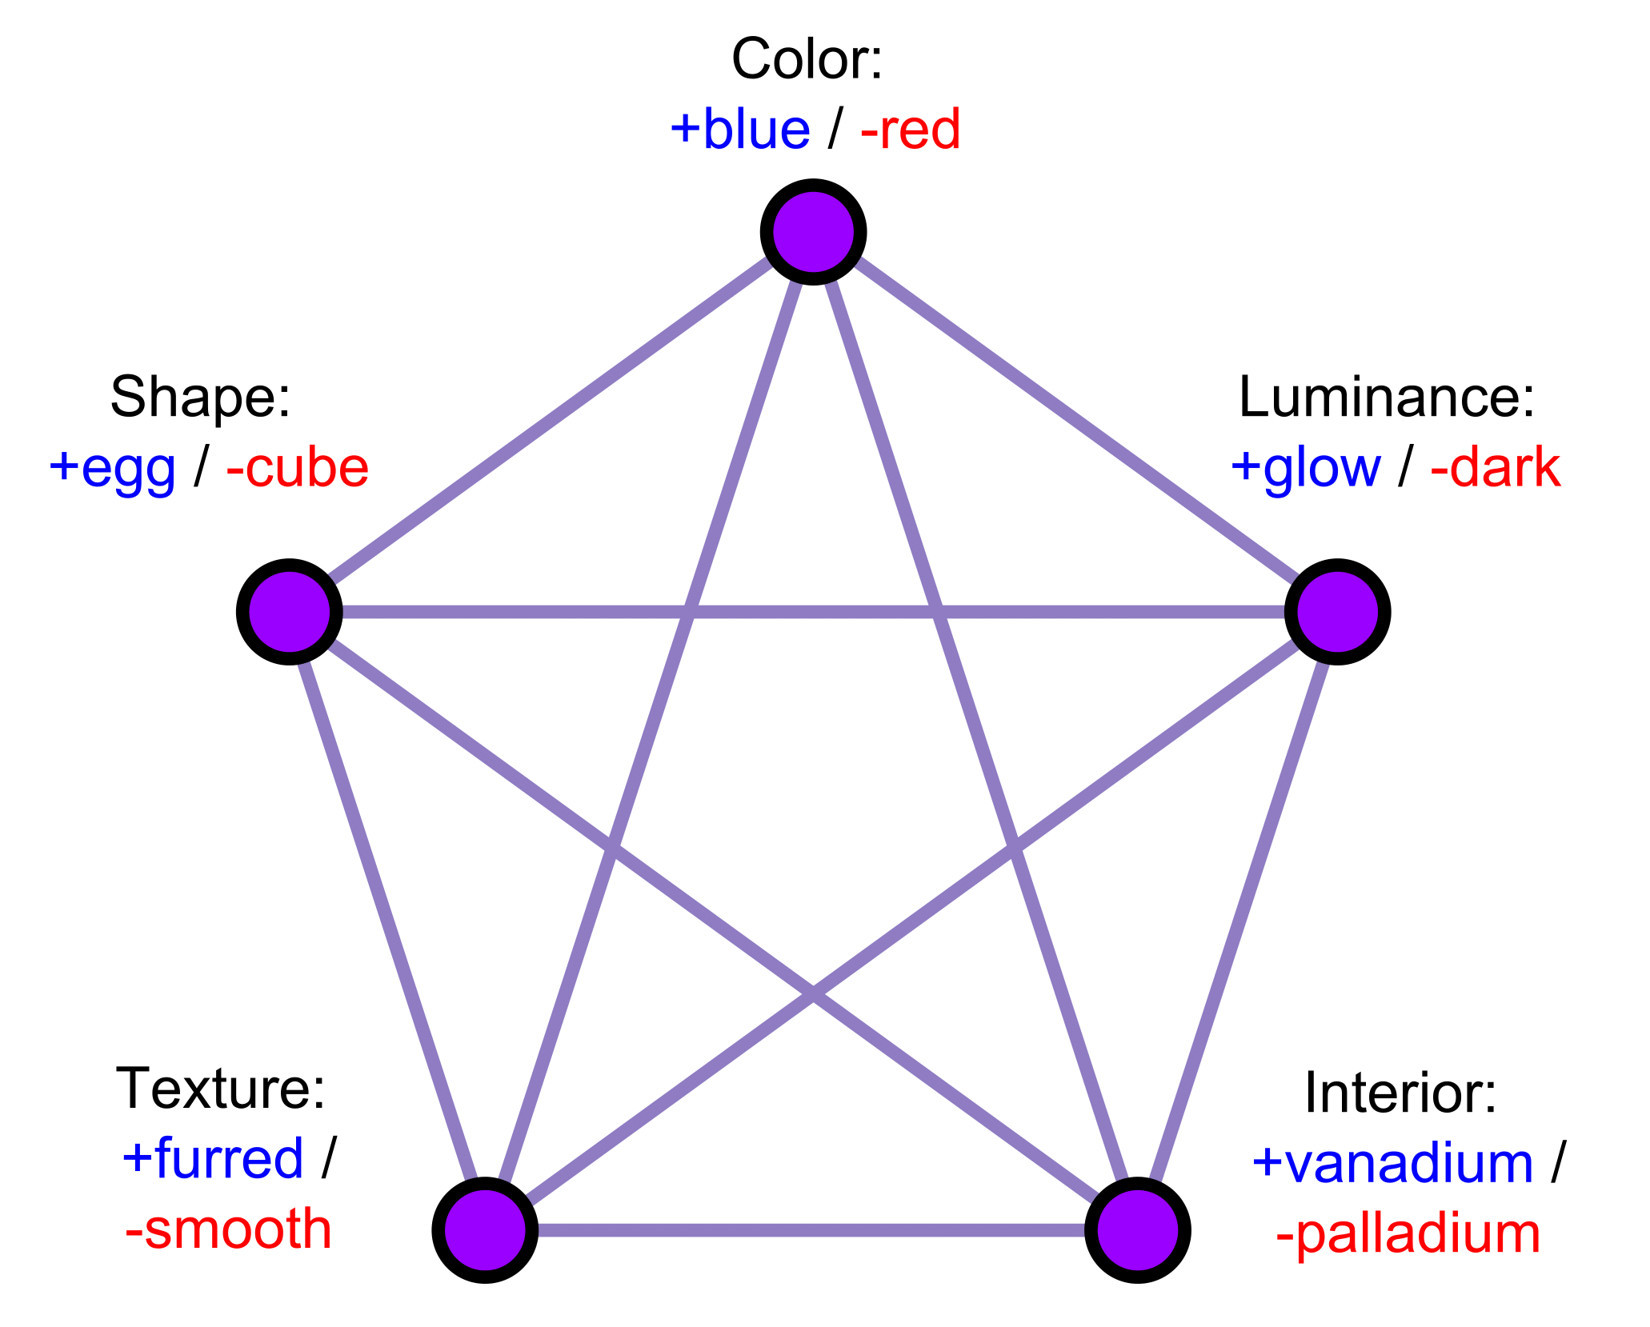
\includegraphics[scale=0.25]{Rationality20From20AI20to20Zombies2020Eliezer20Yudkowsky-img198.jpg}
 \newline
 Figure 161.1: Network 1
\par}


\bigskip

{
\ \ \ ~}

{
\ \ \ Network 1 is for classifying bleggs and rubes. But since
``blegg'' is an unfamiliar and
synthetic concept, I've also included a similar Network
1b in Figure 161.2 for distinguishing humans from Space Monsters, with
input from Aristotle (``All men are
mortal'') and Plato's Academy
(``A featherless biped with broad
nails'').}

{
\ \ \ ~}

{\centering
\ \ \  
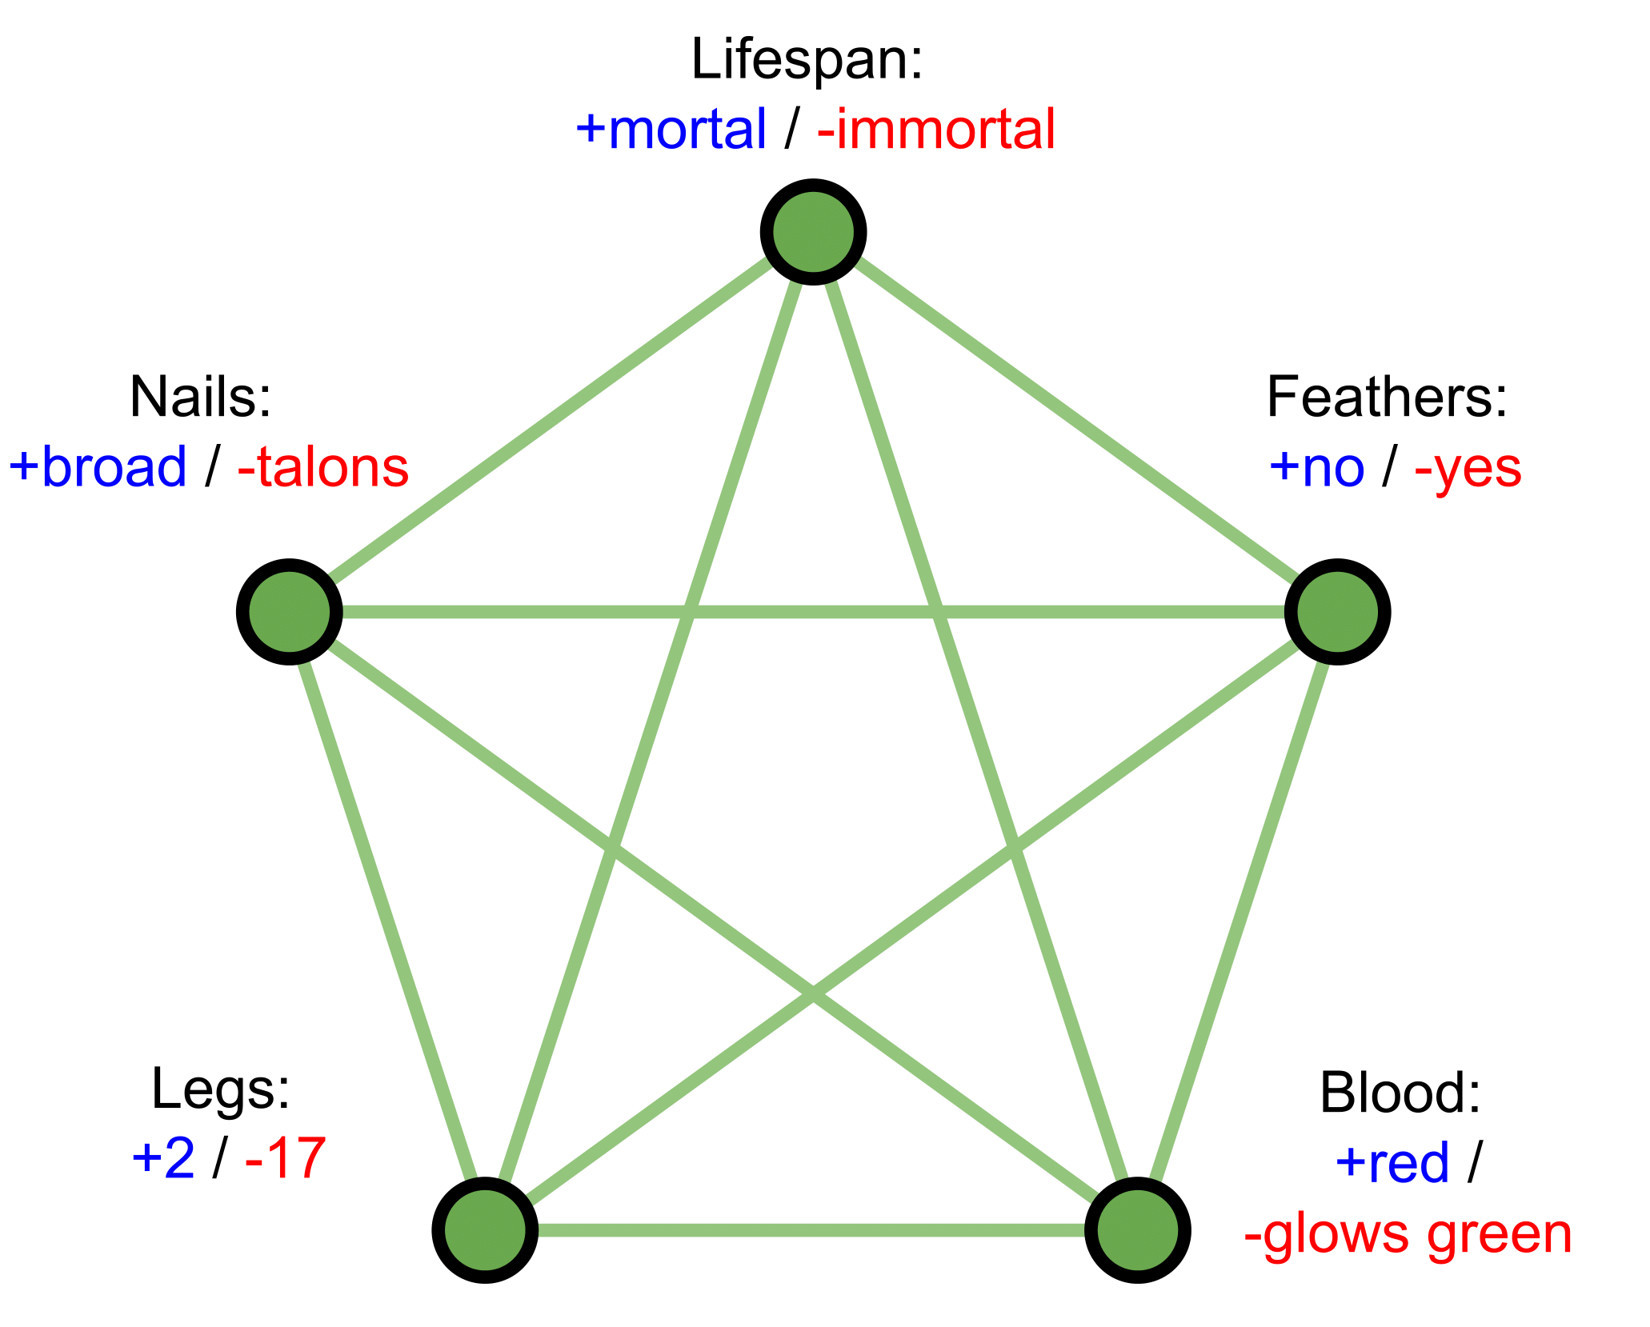
\includegraphics[scale=0.25]{Rationality20From20AI20to20Zombies2020Eliezer20Yudkowsky-img199.jpg}
 \newline
 Figure 161.2: Network 1b
\par}


\bigskip

{
\ \ \ ~}

{
\ \ \ A neural network needs a learning rule. The obvious idea is that
when two nodes are often active at the same time, we should strengthen
the connection between them---this is one of the first rules ever
proposed for training a neural network, known as Hebb's
Rule.}

{
\ \ \ Thus, if you often saw things that were both blue and
furred---thus simultaneously activating the
``color'' node in the + state and
the ``texture'' node in the +
state---the connection would strengthen between color and texture, so
that + colors activated + textures, and vice versa. If you saw things
that were blue and egg-shaped and vanadium-containing, that would
strengthen positive mutual connections between color and shape and
interior.}

{
\ \ \ Let's say you've already seen
plenty of bleggs and rubes come off the conveyor belt. But now you see
something that's furred, egg-shaped,
and---gasp!---reddish purple (which we'll model as a
``color'' activation level of -2/3).
You haven't yet tested the luminance, or the interior.
What to predict, what to predict?}

{
\ \ \ What happens then is that the activation levels in Network 1
bounce around a bit. Positive activation flows to luminance from shape,
negative activation flows to interior from color, negative activation
flows from interior to luminance .~.~. Of course all these messages are
passed in \textit{parallel!!} and \textit{asynchronously!!} just like
the human brain .~.~.}

{
\ \ \ Finally Network 1 settles into a stable state, which has high
positive activation for
``luminance'' and
``interior.'' The network may be
said to ``expect'' (though it has
not yet seen) that the object will glow in the dark, and that it
contains vanadium.}

{
\ \ \ And lo, Network 1 exhibits this behavior even though
there's no explicit node that says whether the object
is a blegg or not. The judgment is \textit{implicit in the whole
network!!} Bleggness is an \textit{attractor!!} which arises as the
result of \textit{emergent behavior!!} from the \textit{distributed!!}
learning rule.}

{
\ \ \ Now in real life, this kind of network design---however faddish it
may sound---runs into \textit{all sorts} of problems. Recurrent
networks don't always settle right away: They can
oscillate, or exhibit chaotic behavior, or just take a very long time
to settle down. This is a Bad Thing when you see something big and
yellow and striped, and you have to wait five minutes for your
distributed neural network to settle into the
``tiger'' attractor. Asynchronous
and parallel it may be, but it's not real-time.}

{
\ \ \ And there are other problems, like double-counting the evidence
when messages bounce back and forth: If you suspect that an object
glows in the dark, your suspicion will activate belief that the object
contains vanadium, which in turn will activate belief that the object
glows in the dark.}

{
\ \ \ Plus if you try to scale up the Network 1 design, it requires
O(N\textsuperscript{2}) connections, where N is the total number of
observables.}

{
\ \ \ So what might be a more realistic neural network design?}

{
\ \ \ ~}

{\centering
\ \ \  
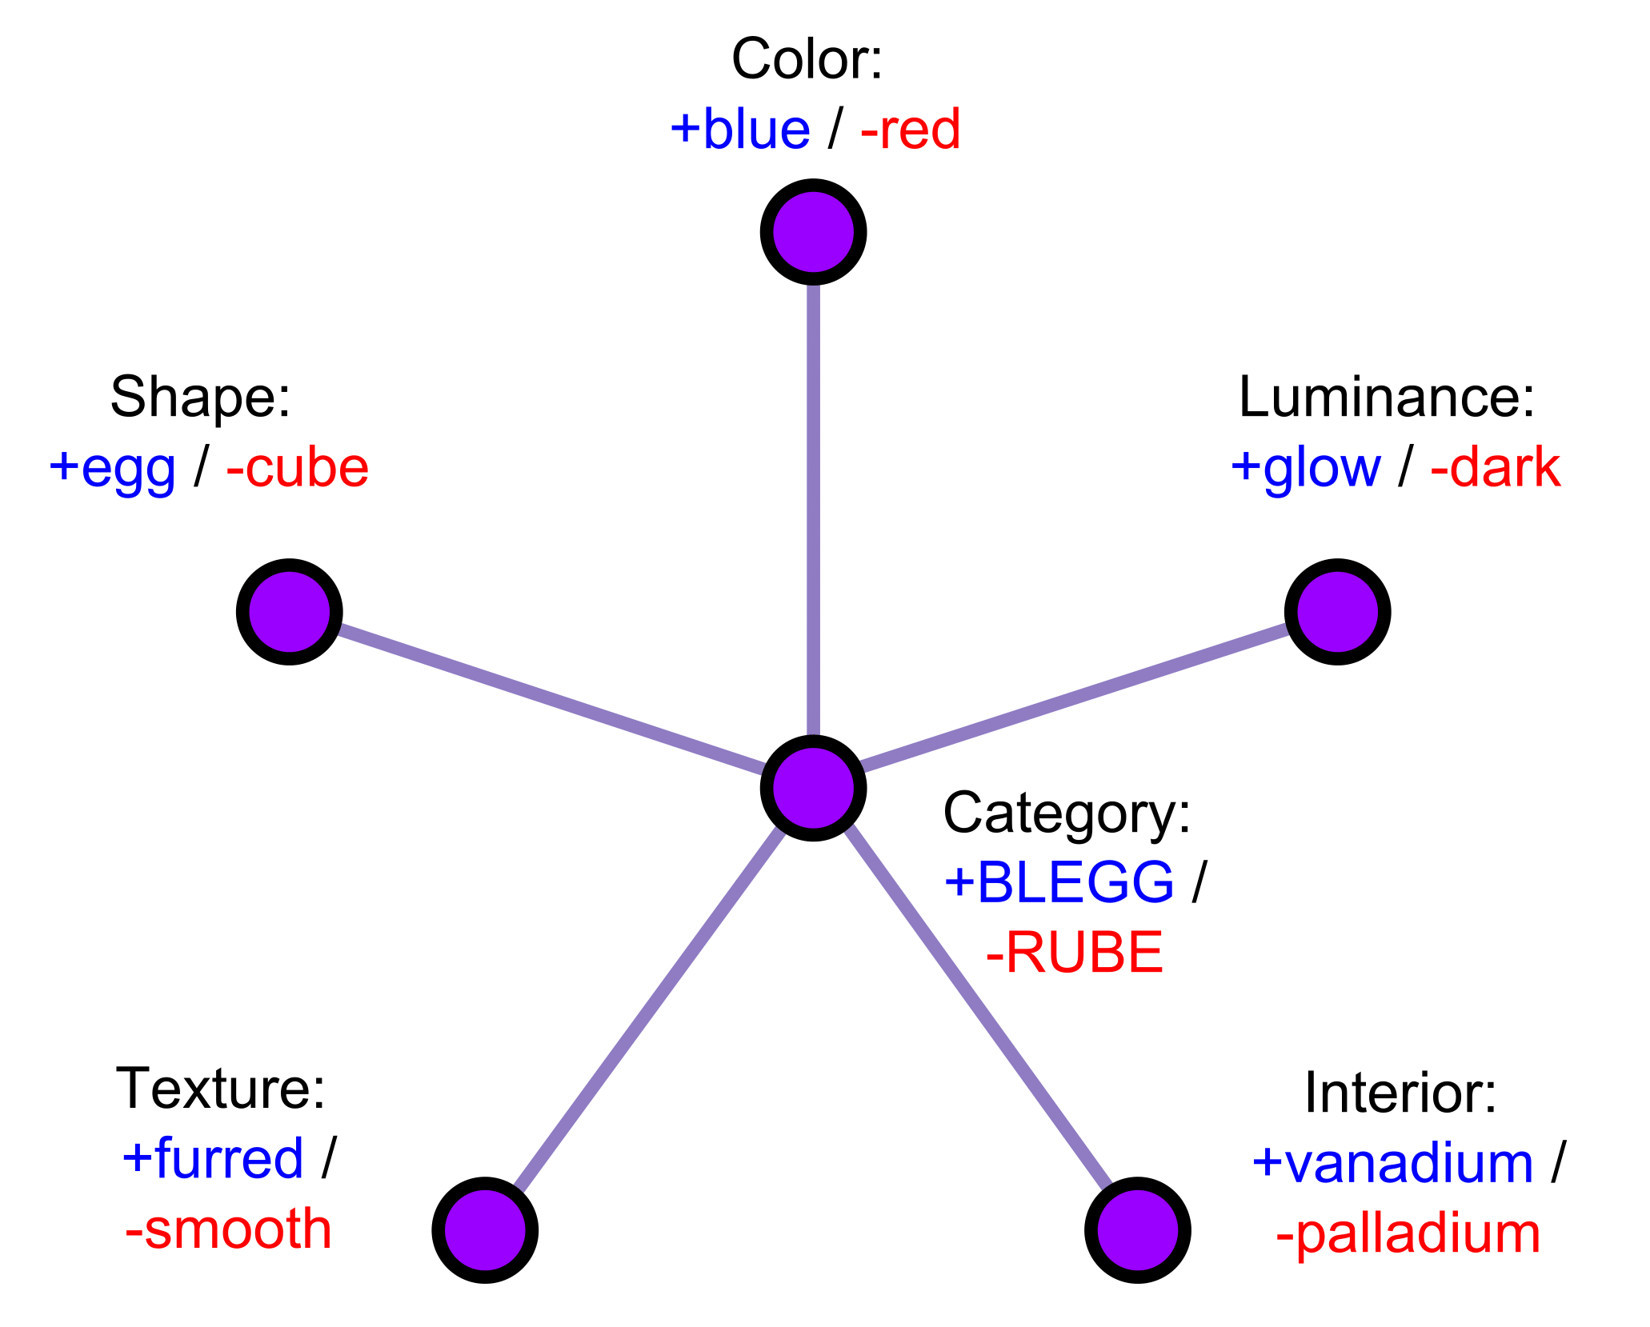
\includegraphics[scale=0.25]{Rationality20From20AI20to20Zombies2020Eliezer20Yudkowsky-img200.jpg}
 \newline
 Figure 161.3: Network 2
\par}


\bigskip

{
\ \ \ ~}

{
\ \ \ In Network 2 of Figure 161.3, a wave of activation converges on
the central node from any clamped (observed) nodes, and then surges
back out again to any unclamped (unobserved) nodes. Which means we can
compute the answer in one step, rather than waiting for the network to
settle---an important requirement in biology when the neurons only run
at 20Hz. And the network architecture scales as O(N), rather than
O(N\textsuperscript{2}).}

{
\ \ \ Admittedly, there are some things you can notice more easily with
the first network architecture than the second. Network 1 has a direct
connection between every two nodes. So if red objects \textit{never}
glow in the dark, but red furred objects usually have the other blegg
characteristics like egg-shape and vanadium, Network 1 can easily
represent this: it just takes a very strong direct negative connection
from color to luminance, but more powerful positive connections from
texture to all other nodes except luminance.}

{
\ \ \ Nor is this a ``special
exception'' to the general rule that bleggs
glow---remember, in Network 1, there is no unit that represents
blegg-ness; blegg-ness emerges as an attractor in the distributed
network.}

{
\ \ \ So yes, those O(N\textsuperscript{2}) connections were buying us
something. But not very much. Network 1 is not \textit{more} useful on
most real-world problems, where you rarely find an animal stuck halfway
between being a cat and a dog.}

{
\ \ \ (There are also facts that you can't easily
represent in Network 1 \textit{or} Network 2. Let's say
sea-blue color and spheroid shape, when found together, always indicate
the presence of palladium; but when found individually, without the
other, they are each very strong evidence for vanadium. This is hard to
represent, in either architecture, without extra nodes. Both Network 1
and Network 2 embody implicit assumptions about what kind of
environmental structure is likely to exist; the ability to read this
off is what separates the adults from the babes, in machine learning.)}

{
\ \ \ Make no mistake: Neither Network 1 nor Network 2 is biologically
realistic. \textit{But} it still seems like a fair guess that however
the brain really works, it is in some sense closer to Network 2 than
Network 1. Fast, cheap, scalable, works well to distinguish dogs and
cats: natural selection goes for that sort of thing like water running
down a fitness landscape.}

{
\ \ \ It seems like an ordinary enough task to classify objects as
either bleggs or rubes, tossing them into the appropriate bin. But
would you notice if sea-blue objects never glowed in the dark?}

{
\ \ \ Maybe, if someone presented you with twenty objects that were
alike only in being sea-blue, and then switched off the light, and none
of the objects glowed. If you got hit over the head with it, in other
words. Perhaps by presenting you with all these sea-blue objects in a
group, your brain forms a new subcategory, and can detect the
``doesn't glow''
characteristic within that subcategory. But you probably
wouldn't notice if the sea-blue objects were scattered
among a hundred other bleggs and rubes. It wouldn't be
\textit{easy} or \textit{intuitive} to notice, the way that
distinguishing cats and dogs is easy and intuitive.}

{
\ \ \ Or: ``Socrates is human, all humans are mortal,
therefore Socrates is mortal.'' How did Aristotle
know that Socrates was human? Well, Socrates had no feathers, and broad
nails, and walked upright, and spoke Greek, and, well, was generally
shaped like a human and acted like one. So the brain decides, once and
for all, that Socrates is human; and from there, infers that Socrates
is mortal like all other humans thus yet observed. It
doesn't seem easy or intuitive to ask how much wearing
clothes, as opposed to using language, is associated with mortality.
Just, ``things that wear clothes and use language are
human'' and ``humans are
mortal.''}

{
\ \ \ Are there biases associated with trying to classify things into
categories once and for all? Of course there are. See e.g. Cultish
Countercultishness.}

{\centering
\ \ \ \ ~
\par}

{\centering
\ \ \ *
\par}

\mysection{How An Algorithm Feels From Inside}

{
\ \ \ ``If a tree falls in the forest, and no one hears
it, does it make a sound?'' I remember seeing an
actual argument get started on this subject---a fully naive argument
that went nowhere near Berkeleian subjectivism. Just:}

{
\ \ \ ``It makes a sound, just like any other falling
tree!''}

{
\ \ \ ``But how can there be a sound that no one
hears?''}

{
\ \ \ The standard rationalist view would be that the first person is
speaking as if ``sound'' means
acoustic vibrations in the air; the second person is speaking as if
``sound'' means an auditory
experience in a brain. If you ask ``Are there acoustic
vibrations?'' or ``Are there
auditory experiences?,'' the answer is at once
obvious. And so the argument is really about the definition of the word
``sound.''}

{
\ \ \ I think the standard analysis is essentially correct. So
let's accept that as a premise, and ask: Why do people
get into such arguments? What's the underlying
psychology?}

{
\ \ \ A key idea of the heuristics and biases program is that mistakes
are often more revealing of cognition than correct answers. Getting
into a heated dispute about whether, if a tree falls in a deserted
forest, it makes a sound, is traditionally considered a mistake.}

{
\ \ \ So what kind of mind design corresponds to that error?}

{
\ \ \ In Disguised Queries I introduced the blegg/rube classification
task, in which Susan the Senior Sorter explains that your job is to
sort objects coming off a conveyor belt, putting the blue eggs or
``bleggs'' into one bin, and the red
cubes or ``rubes'' into the rube
bin. This, it turns out, is because bleggs contain small nuggets of
vanadium ore, and rubes contain small shreds of palladium, both of
which are useful industrially.}

{
\ \ \ Except that around 2\% of blue egg-shaped objects contain
palladium instead. So if you find a blue egg-shaped thing that contains
palladium, should you call it a
``rube'' instead?
You're going to put it in the rube bin---why not call
it a ``rube''?}

{
\ \ \ But when you switch off the light, nearly all bleggs glow faintly
in the dark. And blue egg-shaped objects that contain palladium are
just as likely to glow in the dark as any other blue egg-shaped
object.}

{
\ \ \ So if you find a blue egg-shaped object that contains palladium
and you ask ``Is it a blegg?,'' the
answer depends on what you have to do with the answer. If you ask
``Which bin does the object go
in?,'' then you choose as if the object is a rube.
But if you ask ``If I turn off the light, will it
glow?,'' you predict as if the object is a blegg. In
one case, the question ``Is it a
blegg?'' stands in for the disguised query,
``Which bin does it go in?'' In the
other case, the question ``Is it a
blegg?'' stands in for the disguised query,
``Will it glow in the dark?''}

{
\ \ \ Now suppose that you have an object that is blue and egg-shaped
and contains palladium; and you have already observed that it is
furred, flexible, opaque, and glows in the dark.}

{
\ \ \ This answers \textit{every} query, observes every observable
introduced. There's nothing left for a disguised query
to stand \textit{for}.}

{
\ \ \ So why might someone feel an impulse to go on arguing whether the
object is \textit{really} a blegg?}

{
\ \ \ ~}

{\centering
\ \ \  
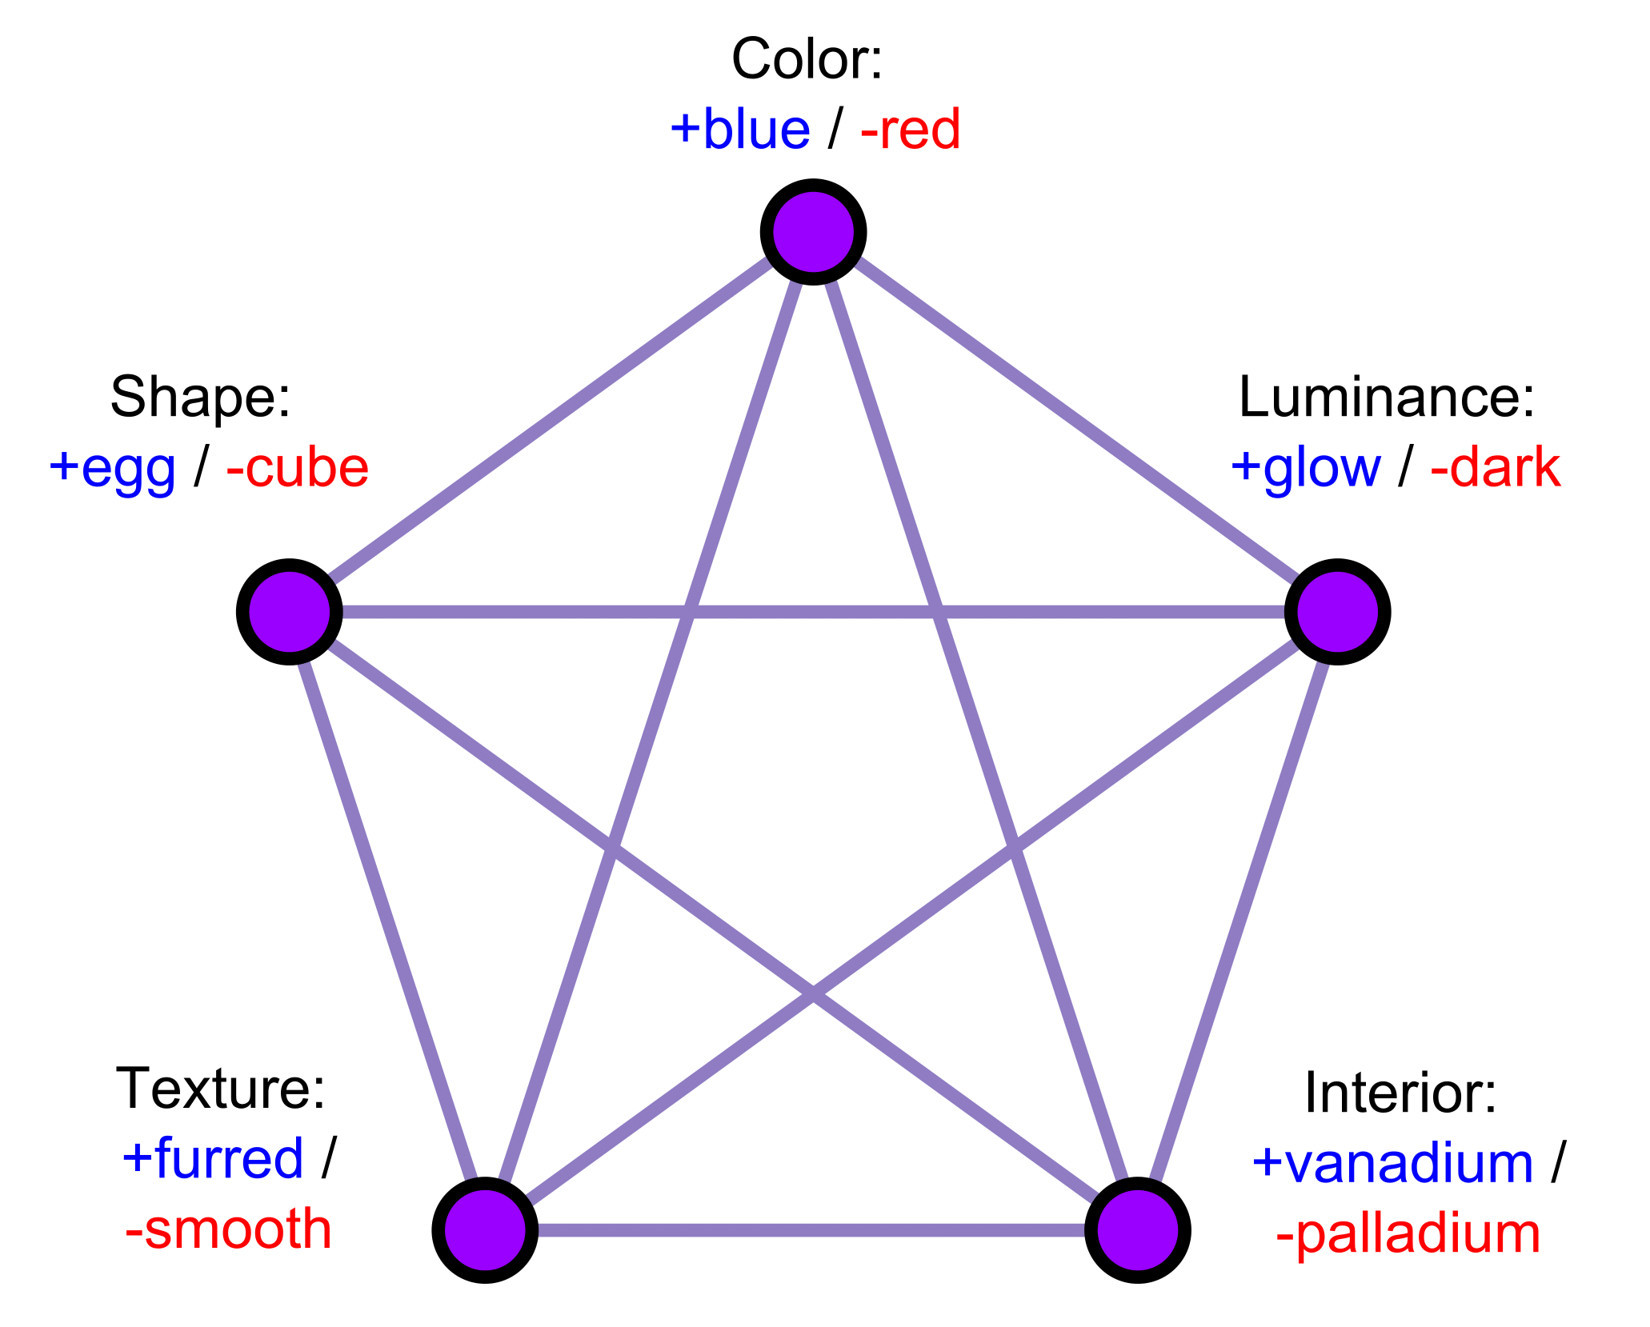
\includegraphics[scale=0.25]{Rationality20From20AI20to20Zombies2020Eliezer20Yudkowsky-img198.jpg}
 \newline
 Figure 162.1: Network 1
\par}


\bigskip

{
\ \ \ ~}

{\centering
\ \ \  
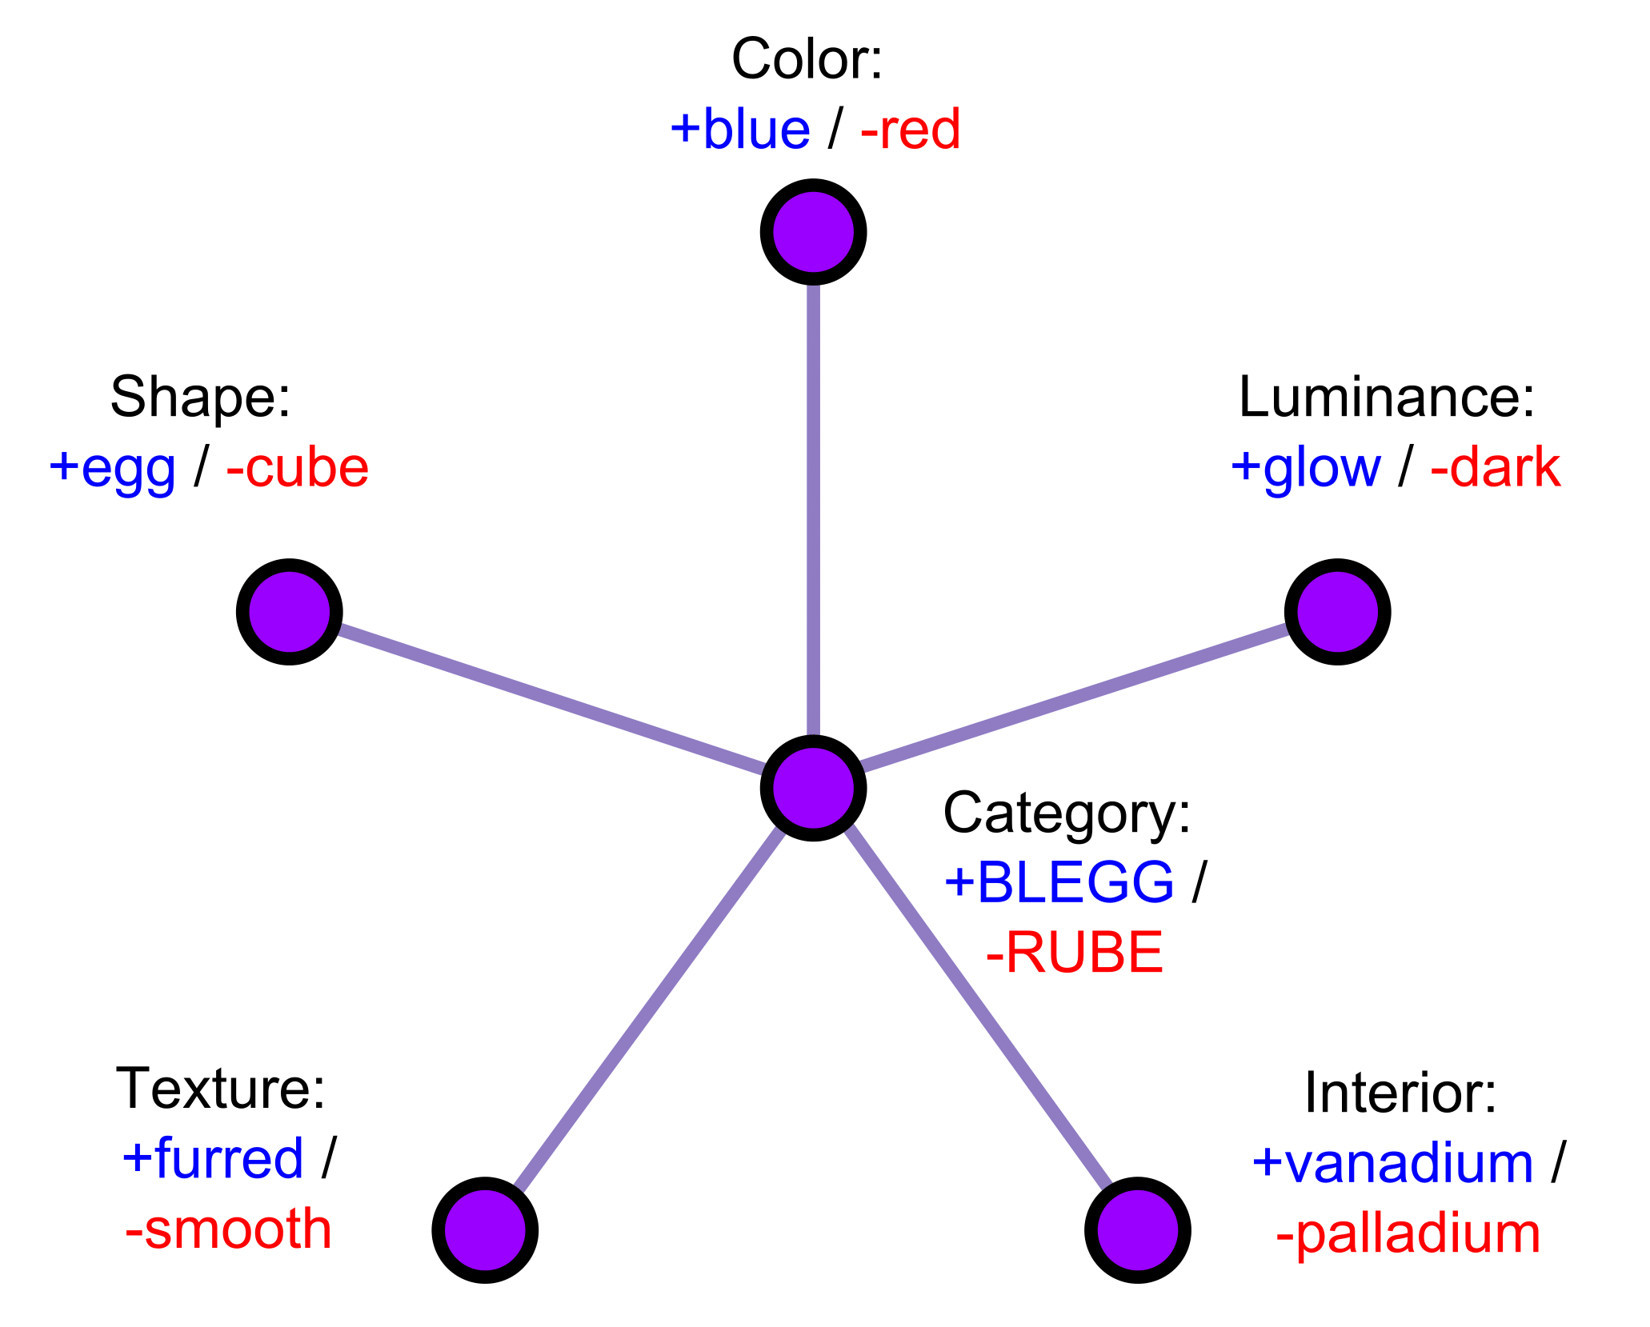
\includegraphics[scale=0.25]{Rationality20From20AI20to20Zombies2020Eliezer20Yudkowsky-img200.jpg}
 \newline
 Figure 162.2: Network 2
\par}


\bigskip

{
\ \ \ ~}

{
\ \ \ These diagrams from Neural Categories show two different neural
networks that might be used to answer questions about bleggs and rubes.
Network 1 (Figure 162.1) has a number of disadvantages---such as
potentially oscillating/chaotic behavior, or requiring
O(N\textsuperscript{2}) connections---but Network 1's
structure does have one major advantage over Network 2: every unit in
the network corresponds to a testable query. If you observe every
observable, clamping every value, there are no units in the network
left over.}

{
\ \ \ Network 2 (Figure 162.2), however, is a far better candidate for
being something vaguely like how the human brain works:
It's fast, cheap, scalable---and has an extra dangling
unit in the center, whose activation can still vary, even after
we've observed every single one of the surrounding
nodes.}

{
\ \ \ Which is to say that even after you know whether an object is blue
or red, egg or cube, furred or smooth, bright or dark, and whether it
contains vanadium or palladium, it \textit{feels} like
there's a leftover, unanswered question: \textit{But is
it really a blegg?}}

{
\ \ \ Usually, in our daily experience, acoustic vibrations and auditory
experience go together. But a tree falling in a deserted forest
unbundles this common association. And even after you know that the
falling tree creates acoustic vibrations but not auditory experience,
it \textit{feels} like there's a leftover question:
\textit{Did it make a sound?}}

{
\ \ \ We know where Pluto is, and where it's going; we
know Pluto's shape, and Pluto's
mass---but is it a planet?}

{
\ \ \ Now remember: When you look at Network 2, as I've
laid it out here, you're seeing the algorithm from the
outside. People don't think to themselves,
``Should the central unit fire, or
not?'' any more than you think
``Should neuron \#12,234,320,242 in my visual cortex
fire, or not?''}

{
\ \ \ It takes a deliberate effort to visualize your brain from the
outside---and then you still don't see your actual
brain; you imagine what you \textit{think} is there. Hopefully based on
science, but regardless, you don't have any direct
access to neural network structures from introspection.
That's why the ancient Greeks didn't
invent computational neuroscience.}

{
\ \ \ When you look at Network 2, you are seeing from the
\textit{outside}; but the way that neural network structure feels from
the \textit{inside}, if you yourself \textit{are} a brain running that
algorithm, is that even after you know every characteristic of the
object, you still find yourself wondering: ``But is it
a blegg, or not?''}

{
\ \ \ This is a great gap to cross, and I've seen it
stop people in their tracks. Because we don't
instinctively see our intuitions as
``intuitions,'' we just see them as
the world. When you look at a green cup, you don't
think of yourself as seeing a picture reconstructed in your visual
cortex---although that \textit{is} what you are seeing---you just see a
green cup. You think, ``Why, look, this cup is
green,'' not, ``The picture in my
visual cortex of this cup is green.''}

{
\ \ \ And in the same way, when people argue over whether the falling
tree makes a sound, or whether Pluto is a planet, they
don't see themselves as arguing over whether a
categorization should be active in their neural networks. It seems like
either the tree makes a sound, or not.}

{
\ \ \ We know where Pluto is, and where it's going; we
know Pluto's shape, and Pluto's
mass---but is it a planet? And yes, there were people who said this was
a fight over definitions---but even that is a Network 2 sort of
perspective, because you're arguing about how the
central unit ought to be wired up. If you were a mind constructed along
the lines of Network 1, you wouldn't say
``It depends on how you define
`planet,''' you would
just say, ``Given that we know Pluto's
orbit and shape and mass, there is no question left to
ask.'' Or, rather, that's how it
would \textit{feel}{}---it would \textit{feel} like there was no
question left---if you were a mind constructed along the lines of
Network 1.}

{
\ \ \ Before you can question your intuitions, you have to realize that
what your mind's eye is looking at \textit{is} an
intuition---some cognitive algorithm, as seen from the inside---rather
than a direct perception of the Way Things Really Are.}

{
\ \ \ People cling to their intuitions, I think, not so much because
they believe their cognitive algorithms are perfectly reliable, but
because they can't see their intuitions \textit{as the
way their cognitive algorithms happen to look from the inside}.}

{
\ \ \ And so everything you try to say about how the native cognitive
algorithm goes astray, ends up being contrasted to their direct
perception of the Way Things Really Are---and discarded as obviously
wrong.}

{\centering
\ \ \ \ ~
\par}

{\centering
\ \ \ *
\par}

\mysection{Disputing Definitions}

{
\ \ \ I have watched more than one conversation---even conversations
supposedly about cognitive science---go the route of disputing over
definitions. Taking the classic example to be ``If a
tree falls in a forest, and no one hears it, does it make a
sound?,'' the dispute often follows a course like
this:}

{
\ \ \ \textit{If a tree falls in the forest, and no one hears it, does
it make a sound?}}

{
\ \ \ ALBERT: ``Of course it does. What kind of silly
question is that? Every time I've listened to a tree
fall, it made a sound, so I'll guess that other trees
falling also make sounds. I don't believe the world
changes around when I'm not
looking.''}

{
\ \ \ BARRY: ``Wait a minute. If no one hears it, how
can it be a sound?''}

{
\ \ \ In this example, Barry is arguing with Albert because of a
genuinely different intuition about what constitutes a sound. But
there's more than one way the Standard Dispute can
start. Barry could have a motive for rejecting Albert's
conclusion. Or Barry could be a skeptic who, upon hearing
Albert's argument, reflexively scrutinized it for
possible logical flaws; and then, on finding a counterargument,
automatically accepted it without applying a second layer of search for
a counter-counterargument; thereby arguing himself into the opposite
position. This doesn't require that
Barry's \textit{prior} intuition---the intuition Barry
would have had, if we'd asked him before Albert
spoke---differs from Albert's.}

{
\ \ \ Well, if Barry didn't have a differing intuition
before, he sure has one now.}

{
\ \ \ ALBERT: ``What do you mean,
there's no sound? The tree's roots
snap, the trunk comes crashing down and hits the ground. This generates
vibrations that travel through the ground and the air.
That's where the energy of the fall goes, into heat and
sound. Are you saying that if people leave the forest, the tree
violates Conservation of Energy?''}

{
\ \ \ BARRY: ``But no one hears anything. If there are
no humans in the forest, or, for the sake of argument, anything else
with a complex nervous system capable of
`hearing,' then no one hears a
sound.''}

{
\ \ \ Albert and Barry recruit arguments that \textit{feel} like support
for their respective positions, describing in more detail the thoughts
that caused their
``sound''-detectors to fire or stay
silent. But so far the conversation has still focused on the forest,
rather than definitions. And note that they don't
actually disagree on anything that happens in the forest.}

{
\ \ \ ALBERT: ``This is the dumbest argument
I've ever been in. You're a
niddlewicking fallumphing pickleplumber.''}

{
\ \ \ BARRY: ``Yeah? Well, you look like your face
caught on fire and someone put it out with a
shovel.''}

{
\ \ \ Insult has been proffered and accepted; now neither party can back
down without losing face. Technically, this isn't part
of the \textit{argument}, as rationalists account such things; but
it's such an important part of the Standard Dispute
that I'm including it anyway.}

{
\ \ \ ALBERT: ``The tree produces acoustic vibrations.
By definition, that is a sound.''}

{
\ \ \ BARRY: ``No one hears anything. By definition,
that is not a sound.''}

{
\ \ \ The argument starts shifting to focus on definitions. Whenever you
feel tempted to say the words ``by
definition'' in an argument that is not literally
about pure mathematics, remember that anything which is true
``by definition'' is true in all
possible worlds, and so observing its truth can never constrain
\textit{which} world you live in.}

{
\ \ \ ALBERT: ``My computer's
microphone can record a sound without anyone being around to hear it,
store it as a file, and it's called a
`sound file.' And what's
stored in the file is the pattern of vibrations in air, not the pattern
of neural firings in anyone's brain.
`Sound' means a pattern of
vibrations.''}

{
\ \ \ Albert deploys an argument that \textit{feels} like support for
the word ``sound'' \textit{having a
particular meaning.} This is a different kind of question from whether
acoustic vibrations take place in a forest---but the shift usually
passes unnoticed.}

{
\ \ \ BARRY: ``Oh, yeah? Let's just see
if the dictionary agrees with you.''}

{
\ \ \ There's a lot of things I could be curious about
in the falling-tree scenario. I could go into the forest and look at
trees, or learn how to derive the wave equation for changes of air
pressure, or examine the anatomy of an ear, or study the neuroanatomy
of the auditory cortex. Instead of doing any of these things, I am to
consult a dictionary, apparently. Why? Are the editors of the
dictionary expert botanists, expert physicists, expert neuroscientists?
Looking in an encyclopedia might make sense, but why a
\textit{dictionary}?}

{
\ \ \ ALBERT: ``Hah! Definition 2c in Merriam-Webster:
`Sound: Mechanical radiant energy that is transmitted by
longitudinal pressure waves in a material medium (as
air).'''}

{
\ \ \ BARRY: ``Hah! Definition 2b in Merriam-Webster:
`Sound: The sensation perceived by the sense of
hearing.'''}

{
\ \ \ ALBERT AND BARRY, CHORUS: ``Consarned dictionary!
This doesn't help at all!''}

{
\ \ \ Dictionary editors are historians of usage, not legislators of
language. Dictionary editors find words in current usage, then write
down the words next to (a small part of) what people seem to mean by
them. If there's more than one usage, the editors write
down more than one definition.}

{
\ \ \ ALBERT: ``Look, suppose that I left a microphone
in the forest and recorded the pattern of the acoustic vibrations of
the tree falling. If I played that back to someone,
they'd call it a
`sound'! That's the
common usage! Don't go around making up your own wacky
definitions!''}

{
\ \ \ BARRY: ``One, I can define a word any way I like
so long as I use it consistently. Two, the meaning I gave was in the
dictionary. Three, who gave you the right to decide what is or
isn't common usage?''}

{
\ \ \ There's quite a lot of rationality errors in the
Standard Dispute. Some of them I've already covered,
and some of them I've yet to cover; likewise the
remedies.}

{
\ \ \ But for now, I would just like to point out---in a mournful sort
of way---that Albert and Barry seem to agree on virtually every
question of what is \textit{actually} going on inside the forest, and
yet it doesn't seem to generate any feeling of
agreement.}

{
\ \ \ Arguing about definitions is a garden path; people
wouldn't go down the path if they saw at the outset
where it led. If you asked Albert (Barry) why he's
still arguing, he'd probably say something like:
``Barry (Albert) is trying to sneak in his own
definition of `sound,' the scurvey
scoundrel, to support his ridiculous point; and I'm
here to defend the standard definition.''}

{
\ \ \ But suppose I went back in time to before the start of the
argument:}

{
\ \ \ \textit{(Eliezer appears from nowhere in a peculiar conveyance
that looks just like the time machine from the original The Time
Machine movie.)}}

{
\ \ \ BARRY: ``Gosh! A time
traveler!''}

{
\ \ \ ELIEZER: ``I am a traveler from the future! Hear
my words! I have traveled far into the past---around fifteen
minutes---''}

{
\ \ \ ALBERT: ``Fifteen
\textit{minutes}?''}

{
\ \ \ ELIEZER: ``---to bring you this
message!''}

{
\ \ \ \textit{(There is a pause of mixed confusion and expectancy.)}}

{
\ \ \ ELIEZER: ``Do you think that
`sound' should be defined to require
both acoustic vibrations (pressure waves in air) and also auditory
experiences (someone to listen to the sound), or should
`sound' be defined as meaning only
acoustic vibrations, or only auditory experience?''}

{
\ \ \ BARRY: ``You went back in time to ask us
\textit{that}?''}

{
\ \ \ ELIEZER: ``My purposes are my own!
Answer!''}

{
\ \ \ ALBERT: ``Well .~.~. I don't see
why it would matter. You can pick any definition so long as you use it
consistently.''}

{
\ \ \ BARRY: ``Flip a coin. Er, flip a coin
twice.''}

{
\ \ \ ELIEZER: ``Personally I'd say
that if the issue arises, both sides should switch to describing the
event in unambiguous lower-level constituents, like acoustic vibrations
or auditory experiences. Or each side could designate a new word, like
`alberzle' and
`bargulum,' to use for what they
respectively used to call `sound'; and
then both sides could use the new words consistently. That way neither
side has to back down or lose face, but they can still communicate. And
of course you should try to keep track, at all times, of some testable
proposition that the argument is actually about. Does that sound right
to you?''}

{
\ \ \ ALBERT: ``I guess .~.~.''}

{
\ \ \ BARRY: ``Why are we talking about
this?''}

{
\ \ \ ELIEZER: ``To preserve your friendship against a
contingency you will, now, never know. For the future has already
changed!''}

{
\ \ \ \textit{(Eliezer and the machine vanish in a puff of smoke.)}}

{
\ \ \ BARRY: ``Where were we
again?''}

{
\ \ \ ALBERT: ``Oh, yeah: If a tree falls in the
forest, and no one hears it, does it make a sound?''}

{
\ \ \ BARRY: ``It makes an alberzle but not a bargulum.
What's the next question?''}

{
\ \ \ This remedy doesn't destroy \textit{every} dispute
over categorizations. But it destroys a substantial fraction.}

{\centering
\ \ \ \ ~
\par}

{\centering
\ \ \ *
\par}

\mysection{Feel the Meaning}

{
\ \ \ When I hear someone say, ``Oh, look, a
butterfly,'' the spoken phonemes
``butterfly'' enter my ear and
vibrate on my ear drum, being transmitted to the cochlea, tickling
auditory nerves that transmit activation spikes to the auditory cortex,
where phoneme processing begins, along with recognition of words, and
reconstruction of syntax (a by no means serial process), and all manner
of other complications. }

{
\ \ \ But at the end of the day, or rather, at the end of the second, I
am primed to look where my friend is pointing and see a visual pattern
that I will recognize as a butterfly; and I would be quite surprised to
see a wolf instead.}

{
\ \ \ My friend looks at a butterfly, his throat vibrates and lips move,
the pressure waves travel invisibly through the air, my ear hears and
my nerves transduce and my brain reconstructs, and lo and behold, I
know what my friend is looking at. Isn't that
marvelous? If we didn't know about the pressure waves
in the air, it would be a tremendous discovery in all the newspapers:
Humans are telepathic! Human brains can transfer thoughts to each
other!}

{
\ \ \ Well, we \textit{are} telepathic, in fact; but magic
isn't exciting when it's merely
\textit{real}, and all your friends can do it too.}

{
\ \ \ Think telepathy is simple? Try building a computer that will be
telepathic with you. Telepathy, or
``language,'' or whatever you want
to call our partial thought transfer ability, is more complicated than
it looks.}

{
\ \ \ But it would be quite inconvenient to go around thinking,
``Now I shall partially transduce some features of my
thoughts into a linear sequence of phonemes which will invoke similar
thoughts in my conversational partner .~.~.''}

{
\ \ \ So the brain hides the complexity---or rather, never represents it
in the first place---which leads people to think some peculiar thoughts
about words.}

{
\ \ \ As I remarked earlier, when a large yellow striped object leaps at
me, I think ``Yikes! A tiger!'' not
``Hm .~.~. objects with the properties of largeness,
yellowness, and stripedness have previously often possessed the
properties `hungry' and
`dangerous,' and therefore, although it
is not logically necessary, \textit{auughhhh} CRUNCH CRUNCH
GULP.''}

{
\ \ \ Similarly, when someone shouts ``Yikes! A
tiger!,'' natural selection would not favor an
organism that thought, ``Hm .~.~. I have just heard
the syllables `Tie' and
`Grr' which my fellow tribe members
associate with their internal analogues of my own \textit{tiger}
concept, and which they are more likely to utter if they see an object
they categorize as \textit{aiiieeee} CRUNCH CRUNCH \textit{help
it's got my arm} CRUNCH GULP.''}

{
\ \ \ ~}

{\centering
\ \ \  
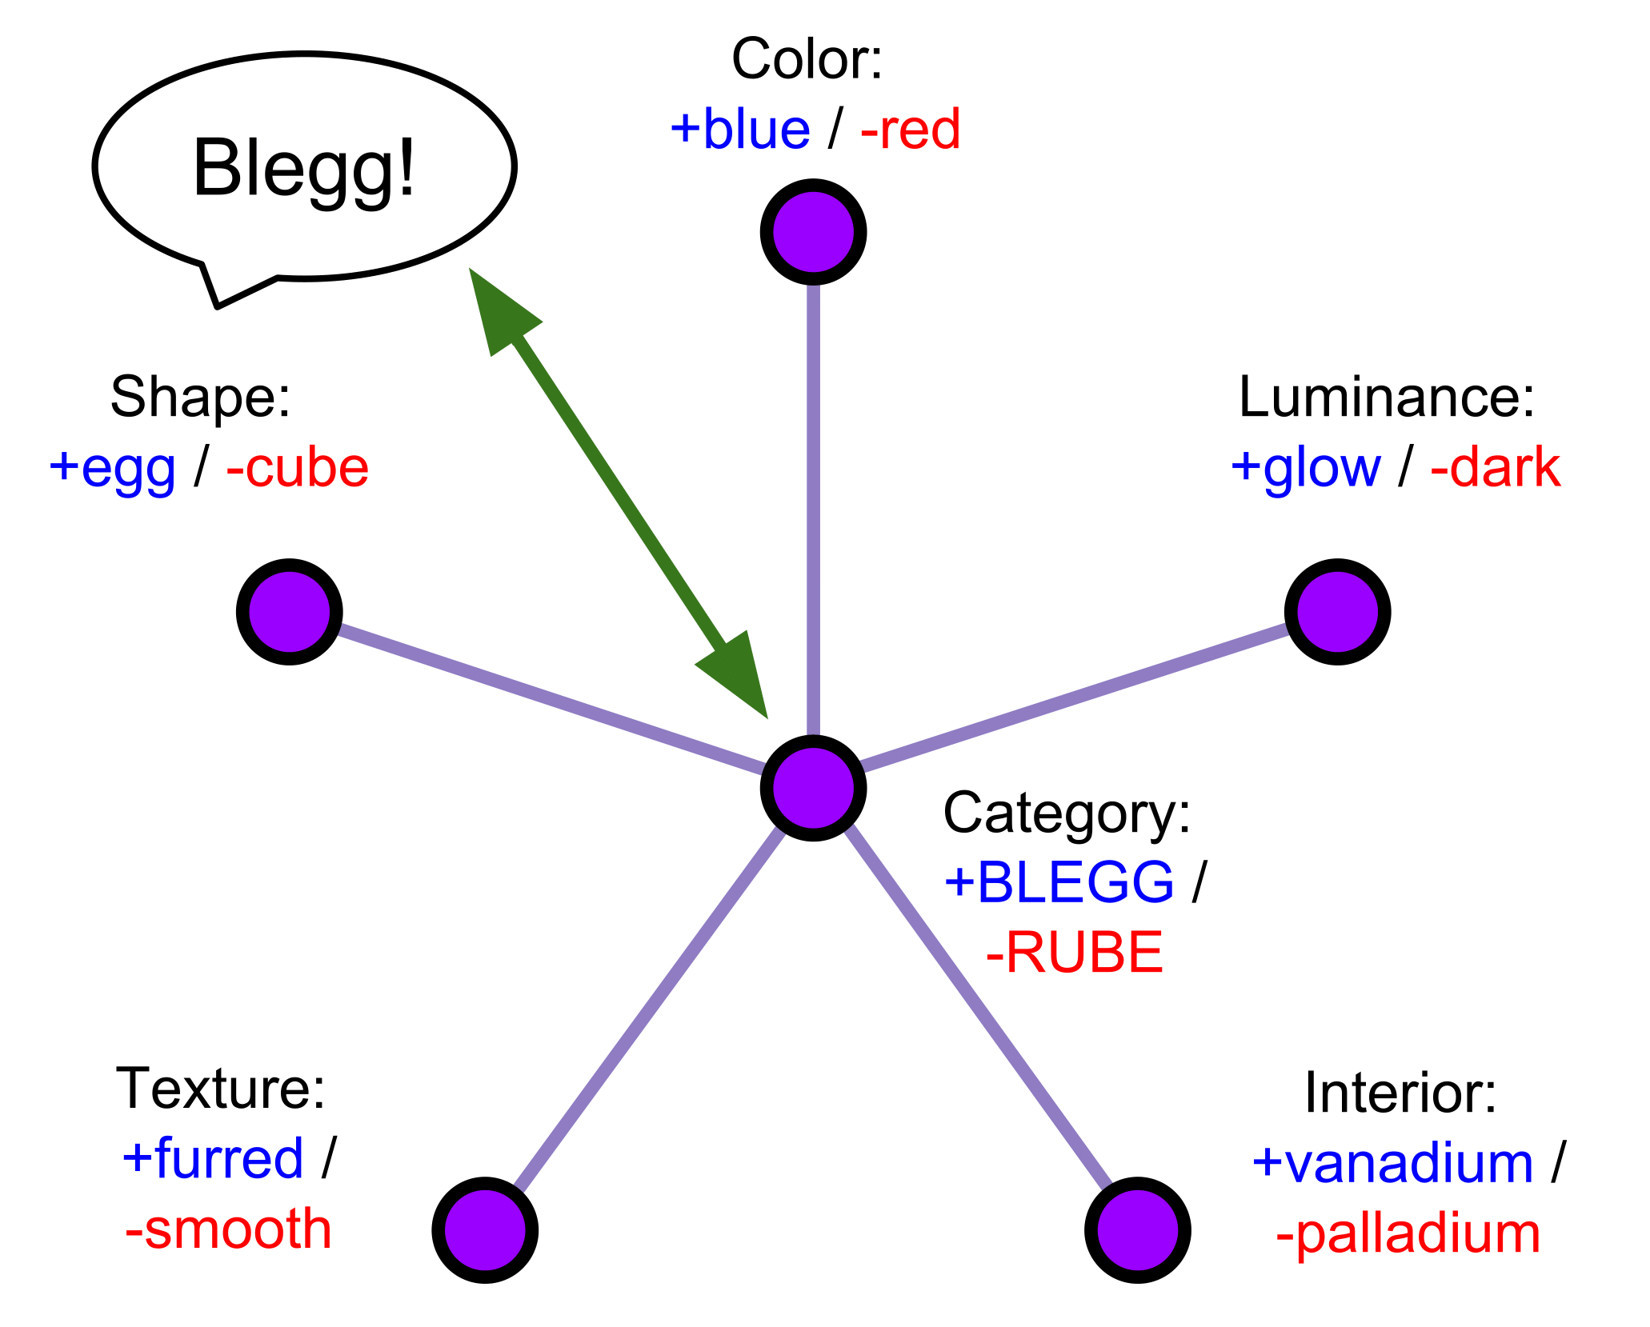
\includegraphics[scale=0.25]{Rationality20From20AI20to20Zombies2020Eliezer20Yudkowsky-img206.jpg}
 \newline
 Figure 164.1: Network 3
\par}


\bigskip

{
\ \ \ ~}

{
\ \ \ Considering this as a design constraint on the human cognitive
architecture, you wouldn't want \textit{any} extra
steps between when your auditory cortex recognizes the syllables
``tiger,'' and when the tiger
concept gets activated.}

{
\ \ \ Going back to the parable of bleggs and rubes, and the centralized
network that categorizes quickly and cheaply, you might visualize a
direct connection running from the unit that recognizes the syllable
``blegg'' to the unit at the center
of the blegg network. The central unit, the blegg concept, gets
activated almost as soon as you hear Susan the Senior Sorter say,
``Blegg!''}

{
\ \ \ Or, for purposes of talking---which also shouldn't
take eons---as soon as you see a blue egg-shaped thing and the central
blegg unit fires, you holler
``Blegg!'' to Susan.}

{
\ \ \ And what that algorithm feels like from inside is that the label,
and the concept, are very nearly \textit{identified}; the meaning
\textit{feels like} an intrinsic property of the word itself.}

{
\ \ \ The cognoscenti will recognize this as a case of E. T.
Jaynes's ``Mind Projection
Fallacy.'' It feels like a word \textit{has a}
meaning, as a property of the word itself; just like how redness is a
property of a red apple, or mysteriousness is a property of a
mysterious phenomenon.}

{
\ \ \ Indeed, on most occasions, the brain will not distinguish at all
between the word and the meaning---only bothering to separate the two
while learning a new language, perhaps. And even then,
you'll see Susan pointing to a blue egg-shaped thing
and saying ``Blegg!,'' and
you'll think, \textit{I wonder what
``blegg'' means,} and not, \textit{I
wonder what mental category Susan associates to the auditory label
``blegg.''}}

{
\ \ \ Consider, in this light, the part of the Standard Dispute of
Definitions where the two parties argue about what the word
``sound'' \textit{really}
means---the same way they might argue whether a particular apple is
\textit{really} red or green:}

{
\ \ \ ALBERT: ``My computer's
microphone can record a sound without anyone being around to hear it,
store it as a file, and it's called a
`sound file.' And what's
stored in the file is the pattern of vibrations in air, not the pattern
of neural firings in anyone's brain.
`Sound' means a pattern of
vibrations.''}

{
\ \ \ BARRY: ``Oh, yeah? Let's just see
if the dictionary agrees with you.''}

{
\ \ \ Albert feels intuitively that the word
``sound'' \textit{has a meaning} and
that the meaning \textit{is} acoustic vibrations. Just as Albert feels
that a tree falling in the forest \textit{makes a sound} (rather than
causing an event that \textit{matches the sound category}).}

{
\ \ \ Barry likewise \textit{feels} that:}

{
\ \ \ sound.meaning == auditory experiences}

{
\ \ \ forest.sound == false.}

{
\ \ \ Rather than:}

{
\ \ \ myBrain.FindConcept({\textquotedbl}sound{\textquotedbl}) ==
concept\_AuditoryExperience}

{
\ \ \ concept\_AuditoryExperience.match(forest) == false.}

{
\ \ \ Which is closer to what's \textit{really} going
on; but humans have not evolved to know this, anymore than humans
instinctively know the brain is made of neurons.}

{
\ \ \ Albert and Barry's conflicting intuitions provide
the fuel for continuing the argument in the phase of arguing over what
the word ``sound'' means---which
\textit{feels} like arguing over a fact like any other fact, like
arguing over whether the sky is blue or green.}

{
\ \ \ You may not even notice that anything has gone astray, until you
try to perform the rationalist ritual of stating a testable experiment
whose result depends on the facts you're so heatedly
disputing .~.~.}

{\centering
\ \ \ \ ~
\par}

{\centering
\ \ \ *
\par}

\mysection{The Argument from Common Usage}

{
\ \ \ Part of the Standard Definitional Dispute runs as follows:}

{
\ \ \ ALBERT: ``Look, suppose that I left a microphone
in the forest and recorded the pattern of the acoustic vibrations of
the tree falling. If I played that back to someone,
they'd call it a
`sound'! That's the
common usage! Don't go around making up your own wacky
definitions!''}

{
\ \ \ BARRY: ``One, I can define a word any way I like
so long as I use it consistently. Two, the meaning I gave was in the
dictionary. Three, who gave you the right to decide what is or
isn't common usage?''}

{
\ \ \ Not all definitional disputes progress as far as recognizing the
notion of common usage. More often, I think, someone picks up a
dictionary because they believe that words have meanings, and the
dictionary faithfully records what this meaning is. Some people even
seem to believe that the dictionary \textit{determines} the
meaning---that the dictionary editors are the Legislators of Language.
Maybe because back in elementary school, their authority-teacher said
that they had to obey the dictionary, that it was a mandatory rule
rather than an optional one?}

{
\ \ \ Dictionary editors read what other people write, and record what
the words seem to mean; they are historians. The Oxford English
Dictionary may be \textit{comprehensive}, but never
\textit{authoritative.}}

{
\ \ \ But surely there is a social imperative to use words in a commonly
understood way? Does not our human telepathy, our valuable power of
language, rely on mutual coordination to work? Perhaps we should
voluntarily treat dictionary editors as supreme arbiters---even if
\textit{they} prefer to think of themselves as historians---in order to
maintain the quiet cooperation on which all speech depends.}

{
\ \ \ The phrase ``authoritative
dictionary'' is almost never used correctly, an
example of proper usage being \textit{The Authoritative Dictionary of
IEEE Standards Terms}. The IEEE is a body of voting members who have a
professional need for exact agreement on terms and definitions, and so
\textit{The Authoritative Dictionary of IEEE Standards Terms} is
actual, negotiated legislation, which exerts whatever authority one
regards as residing in the IEEE.}

{
\ \ \ In everyday life, shared language usually does not arise from a
deliberate agreement, as of the IEEE. It's more a
matter of infection, as words are invented and diffuse through the
culture. (A ``meme,'' one might say,
following Richard Dawkins forty years ago---but you already know what I
mean, and if not, you can look it up on Google, and then you too will
have been infected.)}

{
\ \ \ Yet as the example of the IEEE shows, agreement on language can
also be a cooperatively established public good. If you and I wish to
undergo an exchange of thoughts via language, the human telepathy, then
it is in our mutual interest that we use the \textit{same} word for
similar concepts---preferably, concepts similar to the limit of
resolution in our brain's representation thereof---even
though we have no obvious mutual interest in using any
\textit{particular} word for a concept.}

{
\ \ \ We have no obvious mutual interest in using the word
``oto'' to mean sound, or
``sound'' to mean oto; but we have a
mutual interest in using the \textit{same} word, whichever word it
happens to be. (Preferably, words we use frequently should be short,
but let's not get into information theory just yet.)}

{
\ \ \ But, while we have a mutual interest, it is not strictly
\textit{necessary} that you and I use the similar labels
\textit{internally}; it is only convenient. If I know that, to you,
``oto'' means sound---that is, you
associate ``oto'' to a concept very
similar to the one I associate to
``sound''---then I can say
``Paper crumpling makes a crackling
oto.'' It requires extra thought, but I can do it if
I want.}

{
\ \ \ Similarly, if you say ``What is the walking-stick
of a bowling ball dropping on the floor?'' and I know
which concept \textit{you} associate with the syllables
``walking-stick,'' then I can figure
out what you mean. It may require some thought, and give me pause,
because I ordinarily associate
``walking-stick'' with a different
concept. But I can do it just fine.}

{
\ \ \ When humans really \textit{want} to communicate with each other,
we're hard to stop! If we're stuck on a
deserted island with no common language, we'll take up
sticks and draw pictures in sand.}

{
\ \ \ Albert's appeal to the Argument from Common Usage
assumes that agreement on language is a cooperatively established
public good. Yet Albert assumes this for the sole purpose of
rhetorically accusing Barry of breaking the agreement, and endangering
the public good. Now the falling-tree argument has gone all the way
from botany to semantics to politics; and so Barry responds by
challenging Albert for the authority to define the word.}

{
\ \ \ A rationalist, with the discipline of hugging the query active,
would notice that the conversation had gone rather far astray.}

{
\ \ \ Oh, dear reader, is it all really necessary? Albert knows what
Barry means by ``sound.'' Barry
knows what Albert means by
``sound.'' Both Albert and Barry
have access to words, such as ``acoustic
vibrations'' or ``auditory
experience,'' which they already associate to the
same concepts, and which can describe events in the forest without
ambiguity. If they were stuck on a deserted island, trying to
communicate with each other, their work would be \textit{done}.}

{
\ \ \ When both sides \textit{know} what the other side \textit{wants}
to say, and both sides accuse the other side of defecting from
``common usage,'' then whatever it
is they are about, it is clearly not \textit{working out a way to
communicate with each other.} But this is the whole benefit that common
usage provides in the first place.}

{
\ \ \ Why would you argue about the meaning of a word, two sides trying
to wrest it back and forth? If it's just a namespace
conflict that has gotten blown out of proportion, and nothing more is
at stake, then the two sides need merely generate two new words and use
them consistently.}

{
\ \ \ Yet often categorizations function as hidden inferences and
disguised queries. Is atheism a
``religion''? If someone is arguing
that the reasoning methods used in atheism are on a par with the
reasoning methods used in Judaism, or that atheism is on a par with
Islam in terms of causally engendering violence, then they have a clear
argumentative stake in lumping it all together into an indistinct gray
blur of ``faith.''}

{
\ \ \ Or consider the fight to blend together blacks and whites as
``people.'' This would not be a time
to generate two words---what's at stake is exactly the
idea that you shouldn't draw a moral distinction.}

{
\ \ \ But once any empirical proposition is at stake, \textit{or} any
moral proposition, you can no longer appeal to common usage.}

{
\ \ \ If the question is how to cluster together similar things for
purposes of inference, empirical predictions will depend on the answer;
which means that definitions can be \textit{wrong}. A conflict of
predictions cannot be settled by an opinion poll.}

{
\ \ \ If you want to know whether atheism should be clustered with
supernaturalist religions for purposes of some particular empirical
inference, the dictionary can't answer you.}

{
\ \ \ If you want to know whether blacks are people, the dictionary
can't answer you.}

{
\ \ \ If everyone believes that the red light in the sky is Mars the God
of War, the dictionary will define
``Mars'' as the God of War. If
everyone believes that fire is the release of phlogiston, the
dictionary will define ``fire'' as
the release of phlogiston.}

{
\ \ \ There is an art to using words; even when definitions are not
literally true or false, they are often wiser or more foolish.
Dictionaries are mere histories of past usage; if you treat them as
supreme arbiters of meaning, it binds you to the wisdom of the past,
forbidding you to do better.}

{
\ \ \ Though do take care to ensure (if you must depart from the wisdom
of the past) that people can figure out what you're
trying to swim.}

{\centering
\ \ \ \ ~
\par}

{\centering
\ \ \ *
\par}

\mysection{Empty Labels}

{
\ \ \ Consider (yet again) the Aristotelian idea of categories.
Let's say that there's some object with
properties A, B, C, D, and E, or at least it looks E-ish.}

{
\ \ \ FRED: ``You mean that thing over there is blue,
round, fuzzy, and---''}

{
\ \ \ ME: ``In Aristotelian logic, it's
not supposed to make a difference what the properties are, or what I
call them. That's why I'm just using
the letters.''}

{
\ \ \ Next, I invent the Aristotelian category
``zawa,'' which describes those
objects, all those objects, and only those objects, that have
properties A, C, and D.}

{
\ \ \ ME: ``Object 1 is zawa, B, and
E.''}

{
\ \ \ FRED: ``And it's blue---I mean,
A---too, right?''}

{
\ \ \ ME: ``That's implied when I say
it's zawa.''}

{
\ \ \ FRED: ``Still, I'd like you to
say it explicitly.''}

{
\ \ \ ME: ``Okay. Object 1 is A, B, zawa, and
E.''}

{
\ \ \ Then I add another word,
``yokie,'' which describes all and
only objects that are B and E; and the word
``xippo,'' which describes all and
only objects which are E but not D.}

{
\ \ \ ME: ``Object 1 is zawa and yokie, but not
xippo.''}

{
\ \ \ FRED: ``Wait, is it luminescent? I mean, is it
E?''}

{
\ \ \ ME: ``Yes. That is the only possibility on the
information given.''}

{
\ \ \ FRED: ``I'd rather you spelled it
out.''}

{
\ \ \ ME: ``Fine: Object 1 is A, zawa, B, yokie, C, D,
E, and not xippo.''}

{
\ \ \ FRED: ``Amazing! You can tell all that just by
looking?''}

{
\ \ \ Impressive, isn't it? Let's invent
even more new words: ``Bolo'' is A,
C, and yokie; ``mun'' is A, C, and
xippo; and ``merlacdonian'' is bolo
and mun.}

{
\ \ \ Pointlessly confusing? I think so too. Let's
replace the labels with the definitions:}

{
\ \ \ ``Zawa, B, and E'' becomes [A,
C, D], B, E}

{
\ \ \ ``Bolo and A'' becomes [A, C,
[B, E]], A}

{
\ \ \ ``Merlacdonian'' becomes [A, C,
[B, E]], [A, C, [E, {\textlnot}D]].}

{
\ \ \ And the thing to remember about the Aristotelian idea of
categories is that [A, C, D] is the \textit{entire} information of
``zawa.'' It's not
just that I can vary the label, but that I can get along just fine
without any label at all---the rules for Aristotelian classes work
purely on structures like [A, C, D]. To call one of these structures
``zawa,'' or attach any other label
to it, is a human convenience (or inconvenience) which makes not the
slightest difference to the Aristotelian rules.}

{
\ \ \ Let's say that
``human'' is to be defined as a
mortal featherless biped. Then the classic syllogism would have the
form:}

{
\ \ \ All [mortal, {\textlnot}feathers, bipedal] are mortal.}

{
\ \ \ Socrates is a [mortal, {\textlnot}feathers, bipedal].}

{
\ \ \ Therefore, Socrates is mortal.}

{
\ \ \ The feat of reasoning looks a lot less impressive now,
doesn't it?}

{
\ \ \ Here the \textit{illusion of inference} comes from the labels,
which conceal the premises, and pretend to novelty in the conclusion.
Replacing labels with definitions reveals the illusion, making visible
the tautology's empirical unhelpfulness. You can never
say that Socrates is a [mortal, {\textlnot}feathers, biped] until you
have observed him to be mortal.}

{
\ \ \ There's an idea, which you may have noticed I
hate, that ``you can define a word any way you
like.'' This idea came from the Aristotelian notion
of categories; since, if you follow the Aristotelian rules
\textit{exactly} and \textit{without flaw}{}---which humans never do;
Aristotle knew perfectly well that Socrates was human, even though that
wasn't justified under his rules---but, \textit{if}
some imaginary nonhuman entity were to follow the rules exactly, they
would never arrive at a contradiction. They wouldn't
arrive at much of anything: they couldn't say that
Socrates is a [mortal, {\textlnot}feathers, biped] until they observed
him to be mortal.}

{
\ \ \ But it's not so much that labels are
\textit{arbitrary} in the Aristotelian system, as that the Aristotelian
system works fine without \textit{any labels at all}{}---it cranks out
exactly the same stream of tautologies, they just look a lot less
impressive. The labels are only there to create the \textit{illusion}
of inference.}

{
\ \ \ So if you're going to have an Aristotelian proverb
at all, the proverb should be, not ``I can define a
word any way I like,'' nor even,
``Defining a word never has any
consequences,'' but rather,
``Definitions don't need
words.''}

{\centering
\ \ \ \ ~
\par}

{\centering
\ \ \ *
\par}

\mysection{Taboo Your Words}

{
\ \ \ In the game Taboo (by Hasbro), the objective is for a player to
have their partner guess a word written on a card, without using that
word or five additional words listed on the card. For example, you
might have to get your partner to say
``baseball'' without using the words
``sport,''
``bat,''
``hit,''
``pitch,''
``base'' or of course
``baseball.'' }

{
\ \ \ As soon as I see a problem like that, I at once think,
``An artificial group conflict in which you use a long
wooden cylinder to whack a thrown spheroid, and then run between four
safe positions.'' It might not be the most efficient
strategy to convey the word
``baseball'' under the stated
rules---that might be, ``It's what the
Yankees play''---but the general skill of
\textit{blanking a word out of my mind} was one I'd
practiced for years, albeit with a different purpose.}

{
\ \ \ In the previous essay we saw how replacing terms with definitions
could reveal the empirical unproductivity of the classical Aristotelian
syllogism. All humans are mortal (and also, apparently, featherless
bipeds); Socrates is human; therefore Socrates is mortal. When we
replace the word ``human'' by its
apparent definition, the following underlying reasoning is revealed:}

{
\ \ \ All [mortal, {\textlnot}feathers, biped] are mortal;}

{
\ \ \ Socrates is a [mortal, {\textlnot}feathers, biped];}

{
\ \ \ Therefore Socrates is mortal.}

{
\ \ \ But the principle of replacing words by definitions applies much
more broadly:}

{
\ \ \ ALBERT: ``A tree falling in a deserted forest
makes a sound.''}

{
\ \ \ BARRY: ``A tree falling in a deserted forest does
not make a sound.''}

{
\ \ \ Clearly, since one says
``sound'' and one says
``not sound,'' we must have a
contradiction, right? But suppose that they both dereference their
pointers before speaking:}

{
\ \ \ ALBERT: ``A tree falling in a deserted forest
matches [membership test: this event generates acoustic
vibrations].''}

{
\ \ \ BARRY: ``A tree falling in a deserted forest does
not match [membership test: this event generates auditory
experiences].''}

{
\ \ \ Now there is no longer an apparent collision---all they had to do
was prohibit themselves from using the word \textit{sound}. If
``acoustic vibrations'' came into
dispute, we would just play Taboo again and say
``pressure waves in a material
medium''; if necessary we would play Taboo again on
the word ``wave'' and replace it
with the wave equation. (Play Taboo on ``auditory
experience'' and you get ``That form
of sensory processing, within the human brain, that takes as input a
linear time series of frequency mixes .~.~.'')}

{
\ \ \ But suppose, on the other hand, that Albert and Barry were to have
the argument:}

{
\ \ \ ALBERT: ``Socrates matches the concept
[membership test: this person will die after drinking
hemlock].''}

{
\ \ \ BARRY: ``Socrates matches the concept [membership
test: this person will not die after drinking
hemlock].''}

{
\ \ \ Now Albert and Barry have a substantive clash of expectations; a
difference in what they anticipate seeing after Socrates drinks
hemlock. But they might not notice this, if they happened to use the
same word ``human'' for their
different concepts.}

{
\ \ \ You get a very different picture of what people agree or disagree
about, depending on whether you take a label's-eye-view
(Albert says ``sound'' and Barry
says ``not sound,'' so they must
disagree) or taking the test's-eye-view
(Albert's membership test is acoustic vibrations,
Barry's is auditory experience).}

{
\ \ \ Get together a pack of \textit{soi-disant} futurists and ask them
if they believe we'll have Artificial Intelligence in
thirty years, and I would guess that at least half of them will say
yes. If you leave it at that, they'll shake hands and
congratulate themselves on their consensus. But make the term
``Artificial Intelligence'' taboo,
and ask them to describe \textit{what} they expect to see, without ever
using words like ``computers'' or
``think,'' and you might find quite
a conflict of expectations hiding under that featureless standard word.
See also Shane Legg's compilation of 71 definitions of
``intelligence.''}

{
\ \ \ The illusion of unity across religions can be dispelled by making
the term ``God'' taboo, and asking
them to say what it is they believe in; or making the word
``faith'' taboo, and asking them why
they believe it. Though mostly they won't be able to
answer at all, because it is mostly profession in the first place, and
you cannot cognitively zoom in on an audio recording.}

{
\ \ \ When you find yourself in philosophical difficulties, \textit{the
first line of defense is not to define your problematic terms, but to
see whether you can think without using those terms at all.} Or any of
their short synonyms. And be careful not to let yourself invent a new
word to use instead. Describe outward observables and interior
mechanisms; don't use a single handle, whatever that
handle may be.}

{
\ \ \ Albert says that people have ``free
will.'' Barry says that people don't
have ``free will.'' Well, that will
certainly generate an apparent conflict. Most philosophers would advise
Albert and Barry to try to define exactly what they mean by
``free will,'' on which topic they
will certainly be able to discourse at great length. I would advise
Albert and Barry to describe what it is that they think people do, or
do not have, without using the phrase ``free
will'' at all. (If you want to try this at home, you
should also avoid the words
``choose,''
``act,''
``decide,''
``determined,''
``responsible,'' or any of their
synonyms.)}

{
\ \ \ This is one of the nonstandard tools in my toolbox, and in my
humble opinion, it works \textit{way way} better than the standard one.
It also requires more effort to use; you get what you pay for.}

{\centering
\ \ \ \ ~
\par}

{\centering
\ \ \ *
\par}

\mysection{Replace the Symbol with the Substance}

{
\ \ \ What does it take to---as in the previous essay's
example---see a ``baseball game'' as
``An artificial group conflict in which you use a long
wooden cylinder to whack a thrown spheroid, and then run between four
safe positions''? What does it take to play the
rationalist version of Taboo, in which the goal is not to find a
synonym that isn't on the card, but to find a way of
describing without the standard concept-handle? }

{
\ \ \ You have to visualize. You have to make your
mind's eye see the details, as though looking for the
first time. You have to perform an Original Seeing.}

{
\ \ \ Is that a ``bat''? No,
it's a long, round, tapering, wooden rod, narrowing at
one end so that a human can grasp and swing it.}

{
\ \ \ Is that a ``ball''? No,
it's a leather-covered spheroid with a symmetrical
stitching pattern, hard but not metal-hard, which someone can grasp and
throw, or strike with the wooden rod, or catch.}

{
\ \ \ Are those ``bases''? No,
they're fixed positions on a game field, that players
try to run to as quickly as possible because of their safety within the
game's artificial rules.}

{
\ \ \ The chief obstacle to performing an original seeing is that your
mind already has a nice neat summary, a nice little easy-to-use concept
handle. Like the word ``baseball,''
or ``bat,'' or
``base.'' It takes an effort to stop
your mind from sliding down the familiar path, the easy path, the path
of least resistance, where the small featureless word rushes in and
obliterates the details you're trying to see. A word
itself can have the destructive force of cliché; a word itself can
carry the poison of a cached thought.}

{
\ \ \ Playing the game of Taboo---being able to describe without using
the standard pointer/label/handle---is one of the \textit{fundamental}
rationalist capacities. It occupies the same primordial level as the
habit of constantly asking ``Why?''
or ``What does this belief make me
anticipate?''}

{
\ \ \ The art is closely related to:}

{
\ \ \ Pragmatism, because seeing in this way often gives you a much
closer connection to anticipated experience, rather than propositional
belief;}

{
\ \ \ Reductionism, because seeing in this way often forces you to drop
down to a lower level of organization, look at the parts instead of
your eye skipping over the whole;}

{
\ \ \ Hugging the query, because words often distract you from the
question you really want to ask;}

{
\ \ \ Avoiding cached thoughts, which will rush in using standard words,
so you can block them by tabooing standard words;}

{
\ \ \ The writer's rule of ``Show,
don't tell!,'' which has power among
rationalists;}

{
\ \ \ And not losing sight of your original purpose.}

{
\ \ \ How could tabooing a word help you keep your purpose?}

{
\ \ \ From Lost Purposes:}

{
\ \ \ As you read this, some young man or woman is sitting at a desk in
a university, earnestly studying material they have no intention of
ever using, and no interest in knowing for its own sake. They want a
high-paying job, and the high-paying job requires a piece of paper, and
the piece of paper requires a previous master's degree,
and the master's degree requires a
bachelor's degree, and the university that grants the
bachelor's degree requires you to take a class in
twelfth-century knitting patterns to graduate. So they diligently
study, intending to forget it all the moment the final exam is
administered, but still seriously working away, because they
\textit{want} that piece of paper.}

{
\ \ \ Why are you going to
``school''? To get an
``education'' ending in a
``degree.'' Blank out the forbidden
words and all their obvious synonyms, visualize the actual details, and
you're much more likely to notice that
``school'' currently seems to
consist of sitting next to bored teenagers listening to material you
already know, that a ``degree'' is a
piece of paper with some writing on it, and that
``education'' is forgetting the
material as soon as you're tested on it.}

{
\ \ \ Leaky generalizations often manifest through categorizations:
People who actually learn in classrooms are categorized as
``getting an education,'' so
``getting an education'' must be
good; but then anyone who actually shows up at a college will also
match against the concept ``getting an
education,'' whether or not they learn.}

{
\ \ \ Students who understand math will do well on tests, but if you
require schools to produce good test scores, they'll
spend all their time teaching to the test. A \textit{mental category},
that imperfectly matches your goal, can produce the same kind of
incentive failure \textit{internally.} You want to learn, so you need
an ``education''; and then as long
as you're getting anything that matches against the
category ``education,'' you may not
notice whether you're learning or not. Or
you'll notice, but you won't realize
you've lost sight of your original purpose, because
you're ``getting an
education'' and that's how you
mentally described your goal.}

{
\ \ \ To categorize is to throw away information. If
you're told that a falling tree makes a
``sound,'' you don't
know what the actual sound is; you haven't actually
heard the tree falling. If a coin lands
``heads,'' you don't
know its radial orientation. A blue egg-shaped thing may be a
``blegg,'' but what if the exact egg
shape varies, or the exact shade of blue? You want to use categories to
throw away irrelevant information, to sift gold from dust, but often
the standard categorization ends up throwing out relevant information
too. And when you end up in that sort of mental trouble, the first and
most obvious solution is to play Taboo.}

{
\ \ \ For example: ``Play Taboo'' is
itself a leaky generalization. Hasbro's version is not
the rationalist version; they only list five additional banned words on
the card, and that's not nearly enough coverage to
exclude thinking in familiar old words. What rationalists do would
count as playing Taboo---it would match against the
``play Taboo'' concept---but not
everything that counts as playing Taboo works to force original seeing.
If you just think ``play Taboo to force original
seeing,'' you'll start thinking that
anything that counts as playing Taboo must count as original seeing.}

{
\ \ \ The rationalist version isn't a game, which means
that you can't win by trying to be clever and
stretching the rules. You have to play Taboo with a voluntary handicap:
Stop yourself from using synonyms that aren't on the
card. You also have to stop yourself from inventing a new simple word
or phrase that functions as an equivalent mental handle to the old one.
You are trying to zoom in on your map, not rename the cities;
dereference the pointer, not allocate a new pointer; see the events as
they happen, not rewrite the cliché in a different wording.}

{
\ \ \ By visualizing the problem in more detail, you can see the lost
purpose: Exactly what do you do when you ``play
Taboo''? What purpose does each and every part
serve?}

{
\ \ \ If you see your activities and situation originally, you will be
able to originally see your goals as well. If you can look with fresh
eyes, as though for the first time, you will see yourself doing things
that you would never dream of doing if they were not habits.}

{
\ \ \ Purpose is lost whenever the substance (learning, knowledge,
health) is displaced by the symbol (a degree, a test score, medical
care). To heal a lost purpose, or a lossy categorization, you must do
the reverse:}

{
\ \ \ Replace the symbol with the substance; replace the signifier with
the signified; replace the property with the membership test; replace
the word with the meaning; replace the label with the concept; replace
the summary with the details; replace the proxy question with the real
question; dereference the pointer; drop into a lower level of
organization; mentally simulate the process instead of naming it; zoom
in on your map.}

{
\ \ \ The Simple Truth was generated by an exercise of this discipline
to describe ``truth'' on a lower
level of organization, without invoking terms like
``accurate,''
``correct,''
``represent,''
``reflect,''
``semantic,''
``believe,''
``knowledge,''
``map,'' or
``real.'' (And remember that the
goal is not \textit{really} to play Taboo---the word
``true'' appears in the text, but
\textit{not} to define truth. It would get a buzzer in
Hasbro's game, but we're not
\textit{actually} playing that game. Ask yourself whether the document
fulfilled its purpose, not whether it followed the rules.)}

{
\ \ \ Bayes's Rule itself describes
``evidence'' in pure math, without
using words like ``implies,''
``means,''
``supports,''
``proves,'' or
``justifies.'' Set out to
\textit{define} such philosophical terms, and you'll
just go in circles.}

{
\ \ \ And then there's the most important word of all to
Taboo. I've often warned that you should be careful not
to overuse it, or even avoid the concept in certain cases. Now you know
the real reason why. It's not a bad subject to think
about. But your true understanding is measured by your ability to
describe what you're doing and why, \textit{without}
using that word or any of its synonyms.}

{\centering
\ \ \ \ ~
\par}

{\centering
\ \ \ *
\par}

\mysection{Fallacies of Compression}

{
\ \ \ ``The map is not the
territory,'' as the saying goes. The only life-size,
atomically detailed, 100\% accurate map of California is California.
But California has important regularities, such as the shape of its
highways, that can be described using vastly less information---not to
mention vastly less \textit{physical material}{}---than it would take
to describe every atom within the state borders. Hence the
\textit{other} saying: ``The map is not the territory,
but you can't fold up the territory and put it in your
glove compartment.'' }

{
\ \ \ A paper map of California, at a scale of 10 kilometers to 1
centimeter (a million to one), doesn't have room to
show the distinct position of two fallen leaves lying a centimeter
apart on the sidewalk. Even if the map tried to show the leaves, the
leaves would appear as the same point on the map; or rather the map
would need a feature size of 10 nanometers, which is a finer resolution
than most book printers handle, not to mention human eyes.}

{
\ \ \ Reality is very large---just the part we can see is billions of
lightyears across. But your map of reality is written on a few pounds
of neurons, folded up to fit inside your skull. I don't
mean to be insulting, but your skull is tiny. Comparatively speaking.}

{
\ \ \ Inevitably, then, certain things that are distinct in reality,
will be compressed into the same point on your map.}

{
\ \ \ But what this feels like from inside is not that you say,
``Oh, look, I'm compressing two things
into one point on my map.'' What it \textit{feels}
like from inside is that there is just \textit{one} thing, and you are
seeing it.}

{
\ \ \ A sufficiently young child, or a sufficiently ancient Greek
philosopher, would not know that there were such things as
``acoustic vibrations'' or
``auditory experiences.'' There
would just be a single thing that happened when a tree fell; a single
event called ``sound.''}

{
\ \ \ To realize that there are \textit{two} distinct events, underlying
\textit{one} point on your map, is an essentially \textit{scientific}
challenge---a big, difficult scientific challenge.}

{
\ \ \ Sometimes fallacies of compression result from confusing two known
things under the same label---you know about acoustic vibrations, and
you know about auditory processing in brains, but you call them both
``sound'' and so confuse yourself.
But the more dangerous fallacy of compression arises from having
\textit{no idea whatsoever} that two distinct entities even
\textit{exist}. There is just one mental folder in the filing system,
labeled ``sound,'' and everything
thought about ``sound'' drops into
that one folder. It's not that there are two folders
with the same label; there's just a single folder. By
default, the map is compressed; why would the brain create two mental
buckets where one would serve?}

{
\ \ \ Or think of a mystery novel in which the
detective's critical insight is that one of the
suspects has an identical twin. In the course of the
detective's ordinary work, their job is just to observe
that Carol is wearing red, that she has black hair, that her sandals
are leather---but all these are \textit{facts about} Carol.
It's easy enough to question an individual fact, like
WearsRed(Carol) or BlackHair(Carol). Maybe BlackHair(Carol) is false.
Maybe Carol dyes her hair. Maybe BrownHair(Carol). But it takes a
subtler detective to wonder if the Carol in WearsRed(Carol) and
BlackHair(Carol)---the Carol file into which their observations
drop---should be split into \textit{two} files. Maybe there are two
Carols, so that the Carol who wore red is not the same woman as the
Carol who had black hair.}

{
\ \ \ Here it is the very act of \textit{creating} two different buckets
that is the stroke of genius insight. 'Tis easier to
question one's facts than one's
ontology.}

{
\ \ \ The map of reality contained in a human brain, unlike a paper map
of California, can expand dynamically when we write down more detailed
descriptions. But what this feels like from inside is not so much
zooming in on a map, as fissioning an indivisible atom---taking
\textit{one thing} (it felt like one thing) and splitting it into two
or more things.}

{
\ \ \ Often this manifests in the creation of new words, like
``acoustic vibrations'' and
``auditory experiences'' instead of
just ``sound.'' Something about
creating the new name seems to allocate the new bucket. The detective
is liable to start calling one of their suspects
``Carol-2'' or
``the Other Carol'' almost as soon
as they realize that there are two Carols.}

{
\ \ \ But expanding the map isn't always as simple as
generating new city names. It is a stroke of scientific insight to
realize that such things as acoustic vibrations, or auditory
experiences, even \textit{exist.}}

{
\ \ \ The obvious modern-day illustration would be words like
``intelligence'' or
``consciousness.'' Every now and
then one sees a press release claiming that a research study has
``explained consciousness'' because
a team of neurologists investigated a 40Hz electrical rhythm that might
have something to do with cross-modality binding of sensory
information, or because they investigated the reticular activating
system that keeps humans awake. That's an extreme
example, and the usual failures are more subtle, but they are of the
same kind. The part of
``consciousness'' that people find
most interesting is reflectivity, self-awareness, realizing that the
person I see in the mirror is
``me''; that and the hard problem of
subjective experience as distinguished by David Chalmers. We also label
``conscious'' the state of being
awake, rather than asleep, in our daily cycle. But they are all
different concepts going under the same name, and the underlying
phenomena are different scientific puzzles. You can explain being awake
without explaining reflectivity or subjectivity.}

{
\ \ \ Fallacies of compression also underlie the bait-and-switch
technique in philosophy---you argue about
``consciousness'' under one
definition (like the ability to think about thinking) and then apply
the conclusions to ``consciousness''
under a different definition (like subjectivity). Of course it may be
that the two are the same thing, but if so, genuinely
\textit{understanding} this fact would require \textit{first} a
conceptual split and \textit{then} a genius stroke of reunification.}

{
\ \ \ Expanding your map is (I say again) a \textit{scientific}
challenge: part of the art of science, the skill of inquiring into the
world. (And of course you cannot solve a scientific challenge by
appealing to dictionaries, nor master a complex skill of inquiry by
saying ``I can define a word any way I
like.'') Where you see a single confusing thing, with
protean and self-contradictory attributes, it is a good guess that your
map is cramming too much into one point---you need to pry it apart and
allocate some new buckets. This is not like \textit{defining} the
single thing you see, but it \textit{does} often follow from figuring
out how to talk about the thing without using a single mental handle.}

{
\ \ \ So the skill of prying apart the map is linked to the rationalist
version of Taboo, and to the wise use of words; because words often
represent the points on our map, the labels under which we file our
propositions and the buckets into which we drop our information.
Avoiding a single word, or allocating new ones, is often part of the
skill of expanding the map.}

{\centering
\ \ \ \ ~
\par}

{\centering
\ \ \ *
\par}

\mysection{Categorizing Has Consequences}

{
\ \ \ Among the many genetic variations and mutations you carry in your
genome, there are a very few alleles you probably know---including
those determining your blood type: the presence or absence of the A, B,
and + antigens. If you receive a blood transfusion containing an
antigen you don't have, it will trigger an allergic
reaction. It was Karl Landsteiner's discovery of this
fact, and how to test for compatible blood types, that made it possible
to transfuse blood without killing the patient. (1930 Nobel Prize in
Medicine.) Also, if a mother with blood type A (for example) bears a
child with blood type A+, the mother may acquire an allergic reaction
to the + antigen; if she has another child with blood type A+, the
child will be in danger, unless the mother takes an allergic
suppressant during pregnancy. Thus people learn their blood types
before they marry. }

{
\ \ \ Oh, and \textit{also}: people with blood type A are earnest and
creative, while people with blood type B are wild and cheerful. People
with type O are agreeable and sociable, while people with type AB are
cool and controlled. (You would think that O would be the absence of A
and B, while AB would just be A plus B, but no .~.~.) All this,
according to the Japanese blood type theory of personality. It would
seem that blood type plays the role in Japan that astrological signs
play in the West, right down to blood type horoscopes in the daily
newspaper.}

{
\ \ \ This fad is especially odd because blood types have \textit{never
been} mysterious, not in Japan and not anywhere. We only know blood
types even \textit{exist} thanks to Karl Landsteiner. No mystic witch
doctor, no venerable sorcerer, ever said a word about blood types;
there are no ancient, dusty scrolls to shroud the error in the aura of
antiquity. If the medical profession claimed tomorrow that it had all
been a colossal hoax, we layfolk would not have one scrap of evidence
from our unaided senses to contradict them.}

{
\ \ \ There's never been a war between blood types.
There's never even been a political conflict between
blood types. The stereotypes must have arisen \textit{strictly} from
the \textit{mere existence} of the labels.}

{
\ \ \ Now, someone is bound to point out that this is a story of
categorizing humans. Does the same thing happen if you categorize
plants, or rocks, or office furniture? I can't recall
reading about such an experiment, but of course, that
doesn't mean one hasn't been done.
(I'd expect the chief difficulty of doing such an
experiment would be finding a protocol that didn't
mislead the subjects into thinking that, since the label was given you,
it must be significant somehow.) So while I don't mean
to update on imaginary evidence, I would predict a positive result for
the experiment: I would expect them to find that mere labeling had
power over all things, at least in the human imagination.}

{
\ \ \ You can see this in terms of similarity clusters: once you draw a
boundary around a group, the mind starts trying to harvest similarities
from the group. And unfortunately the human pattern-detectors seem to
operate in such overdrive that we see patterns whether
they're there or not; a weakly negative correlation can
be mistaken for a strong positive one with a bit of selective memory.}

{
\ \ \ You can see this in terms of neural algorithms: creating a name
for a set of things is like allocating a subnetwork to find patterns in
them.}

{
\ \ \ You can see this in terms of a compression fallacy: things given
the same name end up dumped into the same mental bucket, blurring them
together into the same point on the map.}

{
\ \ \ Or you can see this in terms of the boundless human ability to
make stuff up out of thin air and believe it because no one can prove
it's wrong. As soon as you name the category, you can
start making up stuff about it. The named thing doesn't
have to be perceptible; it doesn't have to exist; it
doesn't even have to be coherent.}

{
\ \ \ And no, it's not just Japan: Here in the West, a
blood-type-based diet book called Eat Right 4 Your Type was a
bestseller.}

{
\ \ \ Any way you look at it, drawing a boundary in thingspace is not a
neutral act. Maybe a more cleanly designed, more purely Bayesian AI
could ponder an arbitrary class and not be influenced by it. But you, a
human, do not have that option. Categories are not static things in the
context of a human brain; as soon as you actually think of them, they
exert force on your mind. One more reason not to believe you can define
a word any way you like.}

{\centering
\ \ \ \ ~
\par}

{\centering
\ \ \ *
\par}

\mysection{Sneaking in Connotations}

{
\ \ \ In the previous essay, we saw that in Japan, blood types have
taken the place of astrology---if your blood type is AB, for example,
you're supposed to be ``cool and
controlled.'' }

{
\ \ \ So suppose we decided to invent a new word,
``wiggin,'' and \textit{defined}
this word to mean people with green eyes and black hair---}

{
\ \ \ A green-eyed man with black hair walked into a restaurant.}

{
\ \ \ ``Ha,'' said Danny, watching
from a nearby table, ``did you see that? A wiggin just
walked into the room. Bloody wiggins. Commit all sorts of crimes, they
do.''}

{
\ \ \ His sister Erda sighed. ``You
haven't \textit{seen} him commit any crimes, have you,
Danny?''}

{
\ \ \ ``Don't need
to,'' Danny said, producing a dictionary.
``See, it says right here in the Oxford English
Dictionary. `Wiggin. (1) A person with green eyes and
black hair.' He's got green eyes and
black hair, he's a wiggin. You're not
going to argue with the Oxford English Dictionary, are you? \textit{By
definition,} a green-eyed black-haired person is a
wiggin.''}

{
\ \ \ ``But you called him a
wiggin,'' said Erda.
``That's a nasty thing to say about
someone you don't even know. You've got
no evidence that he puts too much ketchup on his burgers, or that as a
kid he used his slingshot to launch baby
squirrels.''}

{
\ \ \ ``But he \textit{is} a
wiggin,'' Danny said patiently.
``He's got green eyes and black hair,
right? Just you watch, as soon as his burger arrives,
he's reaching for the ketchup.''}

{
\ \ \ The human mind passes from observed characteristics to inferred
characteristics via the medium of words. In ``All
humans are mortal, Socrates is a human, therefore Socrates is
mortal,'' the observed characteristics are
Socrates's clothes, speech, tool use, and generally
human shape; the categorization is
``human''; the inferred
characteristic is poisonability by hemlock.}

{
\ \ \ Of course there's no hard distinction between
``observed characteristics'' and
``inferred characteristics.'' If you
hear someone speak, they're probably shaped like a
human, all else being equal. If you see a human figure in the shadows,
then \textit{ceteris paribus} it can probably speak.}

{
\ \ \ And yet some properties do tend to be more inferred than observed.
You're more likely to decide that someone is human, and
will therefore burn if exposed to open flame, than carry through the
inference the other way around.}

{
\ \ \ If you look in a dictionary for the definition of
``human,'' you're
more likely to find characteristics like
``intelligence'' and
``featherless
biped''---characteristics that are useful for quickly
eyeballing what is and isn't a human---rather than the
ten thousand connotations, from vulnerability to hemlock, to
overconfidence, that we can infer from someone's being
human. Why? Perhaps dictionaries are intended to let you match up
labels to similarity groups, and so are designed to quickly isolate
clusters in thingspace. Or perhaps the big, distinguishing
characteristics are the most salient, and therefore first to pop into a
dictionary editor's mind. (I'm not sure
how aware dictionary editors are of what they \textit{really} do.)}

{
\ \ \ But the upshot is that when Danny pulls out his OED to look up
``wiggin,'' he sees listed only the
first-glance characteristics that distinguish a wiggin: Green eyes and
black hair. The OED doesn't list the many minor
\textit{connotations} that have come to attach to this term, such as
criminal proclivities, culinary peculiarities, and some unfortunate
childhood activities.}

{
\ \ \ How did those connotations get there in the first place? Maybe
there was once a famous wiggin with those properties. Or maybe someone
made stuff up at random, and wrote a series of bestselling books about
it (\textit{The Wiggin}, \textit{Talking to Wiggins}, \textit{Raising
Your Little Wiggin}, \textit{Wiggins in the Bedroom}). Maybe even the
wiggins believe it now, and act accordingly. As soon as you call some
people ``wiggins,'' the word will
begin acquiring connotations.}

{
\ \ \ But remember the Parable of Hemlock: If we go by the logical class
definitions, we can never class Socrates as a
``human'' until after we observe him
to be mortal. Whenever someone pulls a dictionary,
they're generally trying to sneak in a
\textit{connotation}, not the actual definition written down in the
dictionary.}

{
\ \ \ After all, if the \textit{only} meaning of the word
``wiggin'' is
``green-eyed black-haired person,''
then why not just call those people ``green-eyed
black-haired people''? And if you're
wondering whether someone is a ketchup-reacher, why not ask directly,
``Is he a ketchup-reacher?'' rather
than ``Is he a wiggin?'' (Note
substitution of substance for symbol.)}

{
\ \ \ Oh, but arguing the \textit{real} question would require
\textit{work.} You'd have to actually watch the wiggin
to see if he reached for the ketchup. Or maybe see if you can find
statistics on how many green-eyed black-haired people actually like
ketchup. At any rate, you wouldn't be able to do it
sitting in your living room with your eyes closed. And people are lazy.
They'd rather argue ``by
definition,'' especially since they think
``you can define a word any way you
like.''}

{
\ \ \ But of course the \textit{real} reason they care whether someone
is a ``wiggin'' is a connotation---a
feeling that comes along with the word---that isn't in
the definition they \textit{claim} to use.}

{
\ \ \ Imagine Danny saying, ``Look,
he's got green eyes and black hair.
He's a wiggin! It says so right there in the
dictionary!---\textit{therefore,} he's got black hair.
Argue with that, if you can!''}

{
\ \ \ Doesn't have much of a triumphant ring to it, does
it? If the real point of the argument actually \textit{was} contained
in the dictionary definition---if the argument genuinely \textit{was}
logically valid---then the argument would \textit{feel} empty; it would
either say nothing new, or beg the question.}

{
\ \ \ It's only the attempt to smuggle in connotations
\textit{not} explicitly listed in the definition, that makes anyone
feel they can \textit{score a point} that way.}

{\centering
\ \ \ \ ~
\par}

{\centering
\ \ \ *
\par}

\mysection{Arguing ``By Definition''}

{
\ \ \ ``This plucked chicken has two legs and no
feathers---therefore, \textit{by definition,} it is a
human!'' }

{
\ \ \ When people argue definitions, they usually start with some
visible, known, or at least widely believed set of characteristics;
then pull out a dictionary, and point out that these characteristics
fit the dictionary definition; and so conclude,
``Therefore, \textit{by definition,} atheism is a
religion!''}

{
\ \ \ But visible, known, widely believed characteristics are rarely the
real point of a dispute. Just the fact that someone thinks
Socrates's two legs are evident enough to make a good
premise for the argument, ``Therefore, \textit{by
definition,} Socrates is human!'' indicates that
bipedalism probably isn't \textit{really}
what's at stake---or the listener would reply,
``Whaddaya mean Socrates is bipedal?
That's what we're arguing about in the
first place!''}

{
\ \ \ Now there is an important sense in which we can legitimately move
from evident characteristics to not-so-evident ones. You can,
legitimately, see that Socrates is human-shaped, and predict his
vulnerability to hemlock. But this \textit{probabilistic} inference
does not rely on dictionary definitions or common usage; it relies on
the universe containing empirical clusters of similar things.}

{
\ \ \ This cluster structure is not going to change depending on how you
define your words. Even if you look up the dictionary definition of
``human'' and it says
``all featherless bipeds except
Socrates,'' that isn't going to
change the \textit{actual} degree to which Socrates is similar to the
rest of us featherless bipeds.}

{
\ \ \ When you are arguing \textit{correctly} from cluster structure,
you'll say something like, ``Socrates
has two arms, two feet, a nose and tongue, speaks fluent Greek, uses
tools, and in every aspect I've been able to observe
him, seems to have every major and minor property that characterizes
\textit{Homo sapiens}; so I'm going to guess that he
has human DNA, human biochemistry, and is vulnerable to hemlock just
like all other \textit{Homo sapiens} in whom hemlock has been
clinically tested for lethality.''}

{
\ \ \ And suppose I reply, ``But I saw Socrates out in
the fields with some herbologists; I think they were trying to prepare
an antidote. Therefore I \textit{don't} expect Socrates
to keel over after he drinks the hemlock---he will be an exception to
the general behavior of objects in his cluster: they did not take an
antidote, and he did.''}

{
\ \ \ Now there's not much point in arguing over whether
Socrates is ``human'' or not. The
conversation has to move to a more detailed level, poke around
\textit{inside} the details that make up the
``human'' category---talk about
human biochemistry, and specifically, the neurotoxic effects of
coniine.}

{
\ \ \ If you go on insisting, ``But Socrates is a human
and humans, \textit{by definition,} are mortal!''
then what you're really trying to do is blur out
everything you know about Socrates \textit{except} the fact of his
humanity---insist that the only correct prediction is the one you would
make if you knew nothing about Socrates \textit{except} that he was
human.}

{
\ \ \ Which is like insisting that a coin is 50\% likely to be showing
heads or tails, because it is a ``fair
coin,'' after you've \textit{actually
looked at the coin} and it's showing heads.
It's like insisting that Frodo has ten fingers, because
most hobbits have ten fingers, after you've
\textit{already looked at his hands} and seen nine fingers. Naturally
this is illegal under Bayesian probability theory: You
can't just refuse to condition on new evidence.}

{
\ \ \ And you can't just keep one categorization and
make estimates based on that, while deliberately throwing out
everything else you know.}

{
\ \ \ Not every piece of new evidence makes a significant difference, of
course. If I see that Socrates has nine fingers, this
isn't going to noticeably change my estimate of his
vulnerability to hemlock, because I'll expect that the
way Socrates lost his finger didn't change the rest of
his biochemistry. And this is true, \textit{whether or not} the
dictionary's definition says that human beings have ten
fingers. The legal inference is based on the cluster structure of the
environment, and the causal structure of biology; \textit{not} what the
dictionary editor writes down, nor even ``common
usage.''}

{
\ \ \ Now ordinarily, when you're doing this
\textit{right}{}---in a \textit{legitimate} way---you just say,
``The coniine alkaloid found in hemlock produces
muscular paralysis in humans, resulting in death by
asphyxiation.'' Or more simply,
``Humans are vulnerable to
hemlock.'' That's how
it's usually said in a \textit{legitimate} argument.}

{
\ \ \ When would someone feel the need to \textit{strengthen} the
argument with the emphatic phrase ``by
definition''? (E.g. ``Humans are
vulnerable to hemlock \textit{by definition!}'') Why,
when the inferred characteristic has been called into doubt---Socrates
has been seen consulting herbologists---and so the speaker feels the
need to tighten the vise of logic.}

{
\ \ \ So when you see ``by
definition'' used like this, it usually means:
``Forget what you've heard about
Socrates consulting herbologists---humans, \textit{by definition,} are
mortal!''}

{
\ \ \ People feel the need to squeeze the argument onto a single course
by saying ``Any P, by definition, has property
Q!,'' on exactly those occasions when they see, and
prefer to dismiss out of hand, \textit{additional arguments} that call
into doubt the default inference based on clustering.}

{
\ \ \ So too with the argument ``X, \textit{by
definition,} is a Y!'' E.g.,
``Atheists believe that God doesn't
exist; therefore atheists have beliefs about God, because a negative
belief is still a belief; therefore atheism asserts answers to
theological questions; therefore atheism is, \textit{by definition,} a
religion.''}

{
\ \ \ You wouldn't feel the need to say,
``Hinduism, \textit{by definition,} is a
religion!'' because, well, of course Hinduism is a
religion. It's not just a religion
``by definition,''
it's, like, an \textit{actual} religion.}

{
\ \ \ Atheism does not resemble the central members of the
``religion'' cluster, so if it
wasn't for the fact that atheism is a religion
\textit{by definition,} you might go around thinking that atheism
\textit{wasn't} a religion. That's why
you've got to crush all opposition by pointing out that
``Atheism is a religion'' is true
\textit{by definition,} because it isn't true any other
way.}

{
\ \ \ Which is to say: People insist that ``X,
\textit{by definition,} is a Y!'' on those occasions
when they're trying to sneak in a connotation of Y that
isn't directly in the definition, and X
doesn't look all that much like other members of the Y
cluster.}

{
\ \ \ Over the last thirteen years I've been keeping
track of how often this phrase is used correctly versus
incorrectly---though not with literal statistics, I fear. But
eyeballing suggests that using the phrase \textit{by definition,}
anywhere outside of math, is among the most alarming signals of flawed
argument I've ever found. It's right up
there with ``Hitler,''
``God,''
``absolutely certain,'' and
``can't prove
that.''}

{
\ \ \ This heuristic of failure is not perfect---the first time I ever
spotted a correct usage outside of math, it was by Richard Feynman; and
since then I've spotted more. But
you're probably better off just deleting the phrase
``by definition'' from your
vocabulary---and \textit{always} on any occasion where you might be
tempted to say it in italics or followed with an exclamation mark.
That's a bad idea \textit{by definition!}}

{\centering
\ \ \ \ ~
\par}

{\centering
\ \ \ *
\par}

\mysection{Where to Draw the Boundary?}

{
\ \ \ The one comes to you and says:}

{
\ \ \ Long have I pondered the meaning of the word
``Art,'' and at last
I've found what seems to me a satisfactory definition:
``Art is that which is designed for the purpose of
creating a reaction in an audience.''}

{
\ \ \ \textit{Just because there's a word
``art'' doesn't mean
that it }\textbf{\textit{has a meaning}}\textit{, floating out there in
the void, which you can }\textbf{\textit{discover}}\textit{ by finding
the right definition.}}

{
\ \ \ It feels that way, but it is not so.}

{
\ \ \ Wondering how to \textit{define a word} means
you're looking at the problem the wrong way---searching
for the mysterious essence of what is, in fact, a communication
signal.}

{
\ \ \ Now, there \textit{is} a real challenge which a rationalist may
legitimately attack, but the challenge is not to find a satisfactory
definition of a word. The real challenge can be played as a
single-player game, without speaking aloud. The challenge is figuring
out which things are similar to each other---which things are clustered
together---and sometimes, which things have a common cause.}

{
\ \ \ If you define
``eluctromugnetism'' to include
lightning, include compasses, exclude light, and include
Mesmer's ``animal
magnetism'' (what we now call hypnosis), then you
will have some trouble asking ``How does
eluctromugnetism work?'' You have lumped together
things which do not belong together, and excluded others that would be
needed to complete a set. (This example is historically plausible;
Mesmer came before Faraday.)}

{
\ \ \ We could say that eluctromugnetism is a \textit{wrong word}, a
boundary in thingspace that loops around and swerves through the
clusters, a cut that fails to carve reality along its natural joints.}

{
\ \ \ Figuring where to cut reality in order to carve along the
joints---\textit{this} is the problem worthy of a rationalist. It is
what people \textit{should} be trying to do, when they set out in
search of the floating essence of a word.}

{
\ \ \ And make no mistake: it is a \textit{scientific} challenge to
realize that you need a single word to describe breathing and fire. So
do not think to consult the dictionary editors, for that is not their
job.}

{
\ \ \ What is ``art''? But there is
no essence of the word, floating in the void.}

{
\ \ \ Perhaps you come to me with a long list of the things that you
call ``art'' and
``not art'':}

{
\ \ \ The \textit{Little Fugue in G Minor}: Art.}

{
\ \ \ A punch in the nose: Not art.}

{
\ \ \ Escher's \textit{Relativity}: Art.}

{
\ \ \ A flower: Not art.}

{
\ \ \ The Python programming language: Art.}

{
\ \ \ A cross floating in urine: Not art.}

{
\ \ \ Jack Vance's \textit{Tschai} novels: Art.}

{
\ \ \ Modern Art: Not art.}

{
\ \ \ And you say to me: ``It feels intuitive to me to
draw this boundary, but I don't know why---can you find
me an intension that matches this extension? Can you give me a
\textit{simple} description of this boundary?''}

{
\ \ \ So I reply: ``I think it has to do with
admiration of craftsmanship: work going in and wonder coming out. What
the included items have in common is the similar aesthetic emotions
that they inspire, and the deliberate human effort that went into them
with the intent of producing such an emotion.''}

{
\ \ \ Is this helpful, or is it just cheating at Taboo? I would argue
that the list of which human emotions are or are not \textit{aesthetic}
is far more compact than the list of everything that is or
isn't art. You might be able to see those emotions
lighting up an fMRI scan---I say this by way of emphasizing that
emotions are not ethereal.}

{
\ \ \ But of course my definition of art is not the real point. The real
point is that you could well dispute either the intension or the
extension of my definition.}

{
\ \ \ You could say, ``Aesthetic emotion is
\textit{not} what these things have in common; what they have in common
is an intent to inspire \textit{any} complex emotion for the sake of
inspiring it.'' That would be disputing my intension,
my attempt to draw a curve through the data points. You would say,
``Your equation may roughly fit those points, but it
is not the true generating distribution.''}

{
\ \ \ Or you could dispute my extension by saying,
``Some of these things do belong together---I can see
what you're getting at---but the Python language
shouldn't be on the list, and Modern Art should
be.'' (This would mark you as a philistine, but you
could argue it.) Here, the presumption is that there is indeed an
underlying curve that generates this apparent list of similar and
dissimilar things---that there is a rhyme and reason, \textit{even
though you haven't said yet where it comes
from}{}---but I have unwittingly lost the rhythm and included some data
points from a different generator.}

{
\ \ \ Long before you \textit{know} what it is that electricity and
magnetism have in common, you might still suspect---based on surface
appearances---that ``animal
magnetism'' does not belong on the list.}

{
\ \ \ Once upon a time it was thought that the word
``fish'' included dolphins. Now you
could play the oh-so-clever arguer, and say, ``The
list: {\textbackslash}{\textquotesingle}7bSalmon, guppies, sharks,
dolphins, trout{\textbackslash}{\textquotesingle}7d is just a
list---you can't say that a list is \textit{wrong.} I
can prove in set theory that this list exists. So my definition of
\textit{fish}, which is simply this extensional list, cannot possibly
be `wrong' as you
claim.''}

{
\ \ \ Or you could stop playing games and admit that dolphins
don't belong on the fish list.}

{
\ \ \ You come up with a list of things that \textit{feel} similar, and
take a guess at why this is so. But when you finally discover what they
\textit{really} have in common, it may turn out that your guess was
wrong. It may even turn out that your list was wrong.}

{
\ \ \ You cannot hide behind a comforting shield of
correct-by-definition. Both extensional definitions and intensional
definitions can be wrong, can fail to carve reality at the joints.}

{
\ \ \ Categorizing is a guessing endeavor, in which you can make
mistakes; so it's wise to be able to admit, from a
theoretical standpoint, that your definition-guesses can be
``mistaken.''}

{\centering
\ \ \ \ ~
\par}

{\centering
\ \ \ *
\par}

\mysection{Entropy, and Short Codes}

{
\ \ \ (If you aren't familiar with Bayesian inference,
this may be a good time to read An Intuitive Explanation of
Bayes's Theorem.) }

{
\ \ \ Suppose you have a system X that's equally likely
to be in any of 8 possible states:}

{\centering
\ \ \ {\textbackslash}{\textquotesingle}7bX\textsubscript{1},
X\textsubscript{2}, X\textsubscript{3}, X\textsubscript{4},
X\textsubscript{5}, X\textsubscript{6}, X\textsubscript{7},
X\textsubscript{8}{\textbackslash}{\textquotesingle}7d.
\par}


\bigskip

{
\ \ \ There's an extraordinarily ubiquitous
quantity---in physics, mathematics, and even biology---called
\textit{entropy}; and the entropy of X is 3 bits. This means that, on
average, we'll have to ask 3 yes-or-no questions to
find out X's value. For example, someone could tell us
X's value using this code:}

{\centering
\ \ \ X\textsubscript{1} : 001\newline
 X\textsubscript{2} : 010\newline
 X\textsubscript{3} : 011\newline
 X\textsubscript{4} : 100\newline
 X\textsubscript{5} : 101\newline
 X\textsubscript{6} : 110\newline
 X\textsubscript{7} : 111\newline
 X\textsubscript{8} : 000.
\par}


\bigskip

{
\ \ \ So if I asked ``Is the first symbol
1?'' and heard
``yes,'' then asked
``Is the second symbol 1?'' and
heard ``no,'' then asked
``Is the third symbol 1?'' and heard
``no,'' I would know that X was in
state 4.}

{
\ \ \ Now suppose that the system Y has four possible states with the
following probabilities:}

{\centering
\ \ \ Y\textsubscript{1} : 1$/$2 (50\%)\newline
 Y\textsubscript{2} : 1$/$4 (25\%)\newline
 Y\textsubscript{3} : 1$/$8 (12.5\%)\newline
 Y\textsubscript{4} : 1$/$8 (12.5\%).
\par}


\bigskip

{
\ \ \ Then the entropy of Y would be 1.75 bits, meaning that we can find
out its value by asking 1.75 yes-or-no questions.}

{
\ \ \ What does it mean to talk about asking one and three-fourths of a
question? Imagine that we designate the states of Y using the following
code:}

{\centering
\ \ \ Y\textsubscript{1} : 1\newline
 Y\textsubscript{2} : 01\newline
 Y\textsubscript{3} : 001\newline
 Y\textsubscript{4} : 000.
\par}


\bigskip

{
\ \ \ First you ask, ``Is the first symbol
1?'' If the answer is
``yes,'' you're
done: Y is in state 1. This happens half the time, so 50\% of the time,
it takes 1 yes-or-no question to find out Y's state.}

{
\ \ \ Suppose that instead the answer is
``No.'' Then you ask,
``Is the second symbol 1?'' If the
answer is ``yes,''
you're done: Y is in state 2. The system Y is in state
2 with probability 1/4, and each time Y is in state 2 we discover this
fact using two yes-or-no questions, so 25\% of the time it takes 2
questions to discover Y's state.}

{
\ \ \ If the answer is ``No'' twice
in a row, you ask ``Is the third symbol
1?'' If ``yes,''
you're done and Y is in state 3; if
``no,'' you're done
and Y is in state 4. The 1/8 of the time that Y is in state 3, it takes
three questions; and the 1/8 of the time that Y is in state 4, it takes
three questions.}

{\centering
\ \ \ (1/2 {\texttimes} 1) + (1/4 {\texttimes} 2) + (1/8 {\texttimes} 3)
+ (1/8 {\texttimes} 3)
\par}


\bigskip

{\centering
\ \ \ = 0.5 + 0.5 + 0.375 + 0.375
\par}


\bigskip

{\centering
\ \ \ = 1.75.
\par}


\bigskip

{
\ \ \ The general formula for the entropy H(S) of a system S is the sum,
over all S\textsubscript{i}, of
-P(S\textsubscript{i})log\textsubscript{2}(P(S\textsubscript{i})).}

{
\ \ \ For example, the log (base 2) of 1/8 is -3. So -(1$/$8
{\texttimes} -3) = 0.375 is the contribution of state
S\textsubscript{4} to the total entropy: 1/8 of the time, we have to
ask 3 questions.}

{
\ \ \ You can't always devise a perfect code for a
system, but if you have to tell someone the state of arbitrarily many
copies of S in a single message, you can get arbitrarily close to a
perfect code. (Google ``arithmetic
coding'' for a simple method.)}

{
\ \ \ Now, you might ask: ``Why not use the code 10 for
Y\textsubscript{4}, instead of 000? Wouldn't that let
us transmit messages more quickly?''}

{
\ \ \ But if you use the code 10 for Y\textsubscript{4}, then when
someone answers ``Yes'' to the
question ``Is the first symbol 1?,''
you won't know yet whether the system state is
Y\textsubscript{1} (1) or Y\textsubscript{4} (10). In fact, if you
change the code this way, the whole system falls apart---because if you
hear ``1001,'' you
don't know if it means
``Y\textsubscript{4}, followed by
Y\textsubscript{2}'' or
``Y\textsubscript{1}, followed by
Y\textsubscript{3}.''}

{
\ \ \ The moral is that \textit{short words are a conserved resource}.}

{
\ \ \ The key to creating a good code---a code that transmits messages
as compactly as possible---is to reserve short words for things that
you'll need to say frequently, and use longer words for
things that you won't need to say as often.}

{
\ \ \ When you take this art to its limit, the length of the message you
need to describe something corresponds exactly or almost exactly to its
probability. This is the Minimum Description Length or Minimum Message
Length formalization of Occam's Razor.}

{
\ \ \ And so even the \textit{labels} that we use for words are not
quite arbitrary. The sounds that we attach to our concepts can be
better or worse, wiser or more foolish. Even apart from considerations
of common usage!}

{
\ \ \ I say all this, because the idea that ``You can X
any way you like'' is a huge obstacle to learning how
to X wisely. ``It's a free country; I
have a right to my own opinion'' obstructs the art of
finding truth. ``I can define a word any way I
like'' obstructs the art of carving reality at its
joints. And even the sensible-sounding ``The labels we
attach to words are arbitrary'' obstructs awareness
of compactness. Prosody too, for that matter---Tolkien once observed
what a beautiful sound the phrase ``cellar
door'' makes; that is the kind of awareness it takes
to use language like Tolkien.}

{
\ \ \ The length of words also plays a nontrivial role in the cognitive
science of language:}

{
\ \ \ Consider the phrases
``recliner,''
``chair,'' and
``furniture.'' Recliner is a more
specific category than chair; furniture is a more general category than
chair. But the vast majority of chairs have a common use---you use the
same sort of motor actions to sit down in them, and you sit down in
them for the same sort of purpose (to take your weight off your feet
while you eat, or read, or type, or rest). Recliners do not depart from
this theme. ``Furniture,'' on the
other hand, includes things like beds and tables which have different
uses, and call up different motor functions, from chairs.}

{
\ \ \ In the terminology of cognitive psychology,
``chair'' is a \textit{basic-level
category.}}

{
\ \ \ People have a tendency to talk, and presumably think, at the basic
level of categorization---to draw the boundary around
``chairs,'' rather than around the
more specific category ``recliner,''
or the more general category
``furniture.'' People are more
likely to say ``You can sit in that
chair'' than ``You can sit in that
recliner'' or ``You can sit in that
furniture.''}

{
\ \ \ And it is no coincidence that the word for
``chair'' contains fewer syllables
than either ``recliner'' or
``furniture.'' Basic-level
categories, in general, tend to have short names; and nouns with short
names tend to refer to basic-level categories. Not a perfect rule, of
course, but a definite tendency. Frequent use goes along with short
words; short words go along with frequent use.}

{
\ \ \ Or as Douglas Hofstadter put it, there's a reason
why the English language uses
``the'' to mean
``the'' and
``antidisestablishmentarianism'' to
mean
``antidisestablishmentarianism''
instead of antidisestablishmentarianism other way around.}

{\centering
\ \ \ \ ~
\par}

{\centering
\ \ \ *
\par}

\mysection{Mutual Information, and Density in Thingspace}

{
\ \ \ Suppose you have a system X that can be in any of 8 states, which
are all equally probable (relative to your current state of knowledge),
and a system Y that can be in any of 4 states, all equally probable. }

{
\ \ \ The entropy of X, as defined in the previous essay, is 3 bits;
we'll need to ask 3 yes-or-no questions to find out
X's exact state. The entropy of Y is 2 bits; we have to
ask 2 yes-or-no questions to find out Y's exact state.
This may seem obvious since 2\textsuperscript{3} = 8 and
2\textsuperscript{2} = 4, so 3 questions can distinguish 8
possibilities and 2 questions can distinguish 4 possibilities; but
remember that if the possibilities were not all equally likely, we
could use a more clever code to discover Y's state
using e.g. 1.75 questions on average. In this case, though,
X's \textit{probability mass} is \textit{evenly
distributed} over all its possible states, and likewise Y, so we
can't use any clever codes.}

{
\ \ \ What is the entropy of the combined system (X,Y)?}

{
\ \ \ You might be tempted to answer, ``It takes 3
questions to find out X, and then 2 questions to find out Y, so it
takes 5 questions total to find out the state of X and
Y.''}

{
\ \ \ But what if the two variables are entangled, so that learning the
state of Y tells us something about the state of X?}

{
\ \ \ In particular, let's suppose that X and Y are
either both odd or both even.}

{
\ \ \ Now if we receive a 3-bit message (ask 3 questions) and learn that
X is in state X\textsubscript{5}, we know that Y is in state
Y\textsubscript{1} or state Y\textsubscript{3}, but not state
Y\textsubscript{2} or state Y\textsubscript{4}. So the single
additional question ``Is Y in state
Y\textsubscript{3}?,'' answered
``No,'' tells us the entire state of
(X,Y): X = X\textsubscript{5},Y = Y\textsubscript{1}. And we learned
this with a total of 4 questions.}

{
\ \ \ Conversely, if we learn that Y is in state Y\textsubscript{4}
using two questions, it will take us only an additional two questions
to learn whether X is in state X\textsubscript{2}, X\textsubscript{4},
X\textsubscript{6}, or X\textsubscript{8}. Again, four questions to
learn the state of the joint system.}

{
\ \ \ The \textit{mutual information} of two variables is defined as the
difference between the entropy of the joint system and the entropy of
the independent systems: I(X;Y) = H(X) + H(Y) - H(X,Y).}

{
\ \ \ Here there is one bit of mutual information between the two
systems: Learning X tells us one bit of information about Y (cuts down
the space of possibilities from 4 possibilities to 2, a factor-of-2
decrease in the volume) and learning Y tells us one bit of information
about X (cuts down the possibility space from 8 possibilities to 4).}

{
\ \ \ What about when probability mass is not evenly distributed? Last
essay, for example, we discussed the case in which Y had the
probabilities 1/2, 1/4, 1/8, 1/8 for its four states. Let us take this
to be our probability distribution over Y, considered
independently---if we saw Y, without seeing anything else, this is what
we'd expect to see. And suppose the variable Z has two
states, Z\textsubscript{1} and Z\textsubscript{2}, with probabilities
3/8 and 5/8 respectively.}

{
\ \ \ Then if and only if the joint distribution of Y and Z is as
follows, there is zero mutual information between Y and Z:}

{\centering
\ \ \ Z\textsubscript{1}Y\textsubscript{1} : 3/16\newline
 Z\textsubscript{1}Y\textsubscript{2} : 3/32\newline
 Z\textsubscript{1}Y\textsubscript{3} : 3/64\newline
 Z\textsubscript{1}Y\textsubscript{4} : 3/64\newline
 Z\textsubscript{2}Y\textsubscript{1} : 5/16\newline
 Z\textsubscript{2}Y\textsubscript{2} : 5/32\newline
 Z\textsubscript{2}Y\textsubscript{3} : 5/64\newline
 Z\textsubscript{2}Y\textsubscript{4} : 5/64.
\par}


\bigskip

{
\ \ \ This distribution obeys the law}

{\centering
\ \ \ P(Y,Z) = P(Y)P(Z).
\par}


\bigskip

{
\ \ \ For example, P(Z\textsubscript{1}Y\textsubscript{2}) =
P(Z\textsubscript{1})P(Y\textsubscript{2}) = 3$/$8 {\texttimes} 1$/$4 =
3$/$32. }

{
\ \ \ And observe that we can recover the marginal (independent)
probabilities of Y and Z just by looking at the joint distribution:}

{\centering
\ \ \ P(Y\textsubscript{1}) = total probability of all the different
ways Y\textsubscript{1} can happen
\par}


\bigskip

{\centering
\ \ \ = P (Z\textsubscript{1}Y\textsubscript{1}) +
P(Z\textsubscript{2}Y\textsubscript{1})
\par}


\bigskip

{\centering
\ \ \ = 3/16 + 5/16
\par}


\bigskip

{\centering
\ \ \ = 1/2.
\par}


\bigskip

{
\ \ \ So, just by inspecting the joint distribution, we can determine
whether the marginal variables Y and Z are independent; that is,
whether the joint distribution factors into the product of the marginal
distributions; whether, for all Y and Z, we have P(Y,Z) = P(Y)P(Z).}

{
\ \ \ This last is significant because, by Bayes's
Rule,}

{\centering
\ \ \ P(Z\textsubscript{j}Y\textsubscript{i}) =
P(Y\textsubscript{i})P(Z\textsubscript{j})
\par}


\bigskip

{\centering
\ \ \ P(Z\textsubscript{j}Y\textsubscript{i})/P(Z\textsubscript{j}) =
P(Y\textsubscript{i})
\par}


\bigskip

{\centering
\ \ \ P(Y\textsubscript{i}{\textbar}Z\textsubscript{j}) =
P(Y\textsubscript{i}).
\par}


\bigskip

{
\ \ \ In English: ``After you learn Z\textsubscript{j},
your belief about Y\textsubscript{i} is just what it was
before.''}

{
\ \ \ So when the distribution factorizes---when P(Y,Z) =
P(Y)P(Z)---this is \textit{equivalent} to ``Learning
about Y never tells us anything about Z or vice
versa.''}

{
\ \ \ From which you might suspect, correctly, that there is no mutual
information between Y and Z. Where there is no mutual information,
there is no Bayesian evidence, and vice versa.}

{
\ \ \ Suppose that in the distribution (Y,Z) above, we treated each
possible combination of Y and Z as a separate event---so that the
distribution (Y,Z) would have a total of 8 possibilities, with the
probabilities shown---and then we calculated the entropy of the
distribution (Y,Z) the same way we would calculate the entropy of any
distribution:}

{\centering
\ \ \ P(Z\textsubscript{1}Y\textsubscript{1})log\textsubscript{2}(P(Z\textsubscript{1}Y\textsubscript{1}))
+
P(Z\textsubscript{1}Y\textsubscript{2})log\textsubscript{2}(P(Z\textsubscript{1}Y\textsubscript{2}))
+
P(Z\textsubscript{1}Y\textsubscript{3})log\textsubscript{2}(P(Z\textsubscript{1}Y\textsubscript{3}))
+ .~.~. + P
(Z\textsubscript{2}Y\textsubscript{4})log\textsubscript{2}(P(Z\textsubscript{2}Y\textsubscript{4}))
\par}


\bigskip

{\centering
\ \ \ =(3/16)log\textsubscript{2}(3/16) +
(3/32)log\textsubscript{2}(3/32) + (3/64)log\textsubscript{2}(3/64) +
.~.~. + (5/64)log\textsubscript{2}(5/64).
\par}


\bigskip

{
\ \ \ You would end up with the same total you would get if you
separately calculated the entropy of Y plus the entropy of Z. There is
no mutual information between the two variables, so our uncertainty
about the joint system is not any less than our uncertainty about the
two systems considered separately. (I am not showing the calculations,
but you are welcome to do them; and I am not showing the proof that
this is true in general, but you are welcome to Google on
``Shannon entropy'' and
``mutual information.'')}

{
\ \ \ What if the joint distribution doesn't factorize?
For example:}

{\centering
\ \ \ Z\textsubscript{1}Y\textsubscript{1} : 12/64\newline
 Z\textsubscript{1}Y\textsubscript{2} : 8/64\newline
 Z\textsubscript{1}Y\textsubscript{3} : 1/64\newline
 Z\textsubscript{1}Y\textsubscript{4} : 3/64\newline
 Z\textsubscript{2}Y\textsubscript{1} : 20/64\newline
 Z\textsubscript{2}Y\textsubscript{2} : 8/64\newline
 Z\textsubscript{2}Y\textsubscript{3} : 7/64\newline
 Z\textsubscript{2}Y\textsubscript{4} : 5/64.
\par}


\bigskip

{
\ \ \ If you add up the joint probabilities to get marginal
probabilities, you should find that P(Y\textsubscript{1}) = 1$/$2,
P(Z\textsubscript{1}) = 3$/$8, and so on---the marginal probabilities
are the same as before.}

{
\ \ \ But the joint probabilities do not always equal the product of the
marginal probabilities. For example, the probability
P(Z\textsubscript{1}Y\textsubscript{2}) equals 8/64, where
P(Z\textsubscript{1})P(Y\textsubscript{2}) would equal 3$/$8
{\texttimes} 1$/$4 = 6$/$64. That is, the probability of running into
Z\textsubscript{1}Y\textsubscript{2} together is greater than
you'd expect based on the probabilities of running into
Z\textsubscript{1} or Y\textsubscript{2} separately.}

{
\ \ \ Which in turn implies:}

{\centering
\ \ \ P(Z\textsubscript{1}Y\textsubscript{2}) {\textgreater}
P(Z\textsubscript{1})P(Y\textsubscript{2})
\par}


\bigskip

{\centering
\ \ \ P(Z\textsubscript{1}Y\textsubscript{2})/P(Y\textsubscript{2})
{\textgreater} P(Z\textsubscript{1})
\par}


\bigskip

{\centering
\ \ \ P(Z\textsubscript{1}{\textbar}Y\textsubscript{2}) {\textgreater}
P(Z\textsubscript{1}).
\par}


\bigskip

{
\ \ \ Since there's an ``unusually
high'' probability for
P(Z\textsubscript{1}Y\textsubscript{2})---defined as a probability
higher than the marginal probabilities would indicate by default---it
follows that observing Y\textsubscript{2} is evidence that increases
the probability of Z\textsubscript{1}. And by a symmetrical argument,
observing Z\textsubscript{1} must favor Y\textsubscript{2}.}

{
\ \ \ As there are at least some values of Y that tell us about Z (and
vice versa) there must be mutual information between the two variables;
and so you will find---I am confident, though I haven't
actually checked---that calculating the entropy of (Y,Z) yields less
total uncertainty than the sum of the independent entropies of Y and Z.
That is, H(Y,Z) = H(Y) + H(Z) - I(Y;Z), with all quantities necessarily
positive.}

{
\ \ \ (I digress here to remark that the symmetry of the expression for
the mutual information shows that Y \textit{must} tell us as much about
Z, on average, as Z tells us about Y. I leave it as an exercise to the
reader to reconcile this with anything they were taught in logic class
about how, if all ravens are black, being allowed to reason Raven(x)
$\Rightarrow $ Black(x) doesn't mean
you're allowed to reason Black(x) $\Rightarrow $
Raven(x). How different seem the symmetrical probability flows of the
Bayesian, from the sharp lurches of logic---even though the latter is
just a degenerate case of the former.)}

{
\ \ \ ``But,'' you ask,
``what has all this to do with the proper use of
words?''}

{
\ \ \ In Empty Labels and then Replace the Symbol with the Substance, we
saw the technique of replacing a word with its definition---the example
being given:}

{
\ \ \ All [mortal, {\textlnot}feathers, bipedal] are mortal.}

{
\ \ \ Socrates is a [mortal, {\textlnot}feathers, bipedal].}

{
\ \ \ Therefore, Socrates is mortal.}

{
\ \ \ Why, then, would you even want to have a word for
``human''? Why not just say
``Socrates is a mortal featherless
biped''?}

{
\ \ \ Because it's helpful to have shorter words for
things that you encounter often. If your code for describing single
properties is already efficient, then there will not be an advantage to
having a special word for a conjunction---like
``human'' for
``mortal featherless
biped''---unless things that are mortal \textit{and}
featherless \textit{and} bipedal, are found \textit{more often} than
the marginal probabilities would lead you to expect.}

{
\ \ \ In efficient codes, word length corresponds to probability---so
the code for Z\textsubscript{1}Y\textsubscript{2} will be just as long
as the code for Z\textsubscript{1} plus the code for
Y\textsubscript{2}, unless P(Z\textsubscript{1}Y\textsubscript{2})
{\textgreater} P(Z\textsubscript{1})P(Y\textsubscript{2}), in which
case the code for the word can be shorter than the codes for its
parts.}

{
\ \ \ And this in turn corresponds exactly to the case where we can
infer some of the properties of the thing from seeing its other
properties. It must be more likely than the default that featherless
bipedal things will also be mortal.}

{
\ \ \ Of course the word ``human''
really describes many, many more properties---when you see a
human-shaped entity that talks and wears clothes, you can infer whole
hosts of biochemical and anatomical and cognitive facts about it. To
replace the word ``human'' with a
description of everything we know about humans would require us to
spend an inordinate amount of time talking. But this is true
\textit{only} because a featherless talking biped is far more likely
than default to be poisonable by hemlock, or have broad nails, or be
overconfident.}

{
\ \ \ Having a word for a thing, rather than just listing its
properties, is a more compact code precisely in those cases where we
can infer some of those properties from the other properties. (With the
exception perhaps of very primitive words, like
``red,'' that we would use to send
an entirely uncompressed description of our sensory experiences. But by
the time you encounter a bug, or even a rock, you're
dealing with nonsimple property collections, far above the primitive
level.)}

{
\ \ \ So having a word ``wiggin'' for
green-eyed black-haired people is more useful than just saying
``green-eyed black-haired person''
precisely when:}

{
\ \ \ Green-eyed people are more likely than average to be black-haired
(and vice versa), meaning that we can probabilistically infer green
eyes from black hair or vice versa; \textit{or}}

{
\ \ \ Wiggins share other properties that can be inferred at
greater-than-default probability. In this case we have to separately
observe the green eyes and black hair; but then, after observing both
these properties independently, we can probabilistically infer other
properties (like a taste for ketchup).}

{
\ \ \ One may even consider the act of defining a word as a promise to
this effect. Telling someone, ``I define the word
`wiggin' to mean a person with green
eyes and black hair,'' by Gricean implication,
asserts that the word ``wiggin''
will somehow help you make inferences / shorten your messages.}

{
\ \ \ If green-eyes and black hair have no greater than default
probability to be found together, nor does any other property occur at
greater than default probability along with them, then the word
``wiggin'' is a lie: The word claims
that certain people are worth distinguishing as a group, but
they're not.}

{
\ \ \ In this case the word
``wiggin'' does not help describe
reality more compactly---it is not defined by someone sending the
shortest message---it has no role in the simplest explanation.
Equivalently, the word ``wiggin''
will be of no help to you in doing any Bayesian inference. Even if you
do not call the word a lie, it is surely an error.}

{
\ \ \ And the way to carve reality at its joints is to draw your
boundaries around concentrations of unusually high probability density
in Thingspace.}

{\centering
\ \ \ \ ~
\par}

{\centering
\ \ \ *
\par}

\mysection{Superexponential Conceptspace, and Simple Words}

{
\ \ \ Thingspace, you might think, is a rather huge space. Much larger
than reality, for where reality only contains things that actually
exist, Thingspace contains everything that \textit{could} exist. }

{
\ \ \ Actually, the way I ``defined''
Thingspace to have dimensions for every possible attribute---including
correlated attributes like density and volume and mass---Thingspace may
be too poorly defined to have anything you could call a \textit{size}.
But it's important to be able to visualize Thingspace
\textit{anyway}. Surely, no one can \textit{really} understand a flock
of sparrows if all they see is a cloud of flapping cawing things,
rather than a cluster of points in Thingspace.}

{
\ \ \ But as vast as Thingspace may be, it doesn't hold
a candle to the size of Conceptspace.}

{
\ \ \ ``Concept,'' in machine
learning, means a rule that includes or excludes examples. If you see
the data {\textbackslash}{\textquotesingle}7b2:+, 3:-, 14:+, 23:-, 8:+,
9:-{\textbackslash}{\textquotesingle}7d then you might guess that the
concept was ``even numbers.'' There
is a rather large literature (as one might expect) on how to learn
concepts from data .~.~. given random examples, given chosen examples
.~.~. given possible errors in classification .~.~. and most
importantly, given different spaces of possible rules.}

{
\ \ \ Suppose, for example, that we want to learn the concept
``good days on which to play
tennis.'' The possible attributes of Days are}

{\centering
\ \ \ Sky: {\textbackslash}{\textquotesingle}7bSunny, Cloudy,
Rainy{\textbackslash}{\textquotesingle}7d\newline
 AirTemp: {\textbackslash}{\textquotesingle}7bWarm,
Cold{\textbackslash}{\textquotesingle}7d\newline
 Humidity: {\textbackslash}{\textquotesingle}7bNormal,
High{\textbackslash}{\textquotesingle}7d\newline
 Wind: {\textbackslash}{\textquotesingle}7bStrong,
Weak{\textbackslash}{\textquotesingle}7d.
\par}


\bigskip

{
\ \ \ We're then presented with the following data,
where + indicates a positive example of the concept, and - indicates a
negative classification:}

{\centering
\ \ \ + Sky: Sunny; AirTemp: Warm; Humidity: High; Wind: Strong.\newline
 - Sky: Rainy; AirTemp: Cold; Humidity: High; Wind: Strong.\newline
 + Sky: Sunny; AirTemp: Warm; Humidity: High; Wind: Weak.
\par}


\bigskip

{
\ \ \ What should an algorithm infer from this?}

{
\ \ \ A machine learner might represent \textit{one} concept that fits
this data as follows:}

{\centering
\ \ \ {\textbackslash}{\textquotesingle}7bSky: ?; AirTemp: Warm;
Humidity: High; Wind: ?{\textbackslash}{\textquotesingle}7d.
\par}


\bigskip

{
\ \ \ In this format, to determine whether this concept accepts or
rejects an example, we compare element-by-element: ? accepts anything,
but a specific value accepts only that specific value.}

{
\ \ \ So the concept above will accept only Days with AirTemp = Warm and
Humidity = High, but the Sky and the Wind can take on any value. This
fits both the negative and the positive classifications in the data so
far---though it isn't the \textit{only} concept that
does so.}

{
\ \ \ We can also simplify the above concept representation to}

{\centering
\ \ \ {\textbackslash}{\textquotesingle}7b?, Warm, High,
?{\textbackslash}{\textquotesingle}7d.
\par}


\bigskip

{
\ \ \ Without going into details, the classic algorithm would be:}

{
\ \ \ Maintain the set of the most general hypotheses that fit the
data---those that positively classify as many examples as possible,
while still fitting the facts.}

{
\ \ \ Maintain another set of the most specific hypotheses that fit the
data---those that negatively classify as many examples as possible,
while still fitting the facts.}

{
\ \ \ Each time we see a new negative example, we strengthen all the
most general hypotheses as little as possible, so that the new set is
again as general as possible while fitting the facts.}

{
\ \ \ Each time we see a new positive example, we relax all the most
specific hypotheses as little as possible, so that the new set is again
as specific as possible while fitting the facts.}

{
\ \ \ We continue until we have only a single hypothesis left. This will
be the answer \textit{if} the target concept was in our hypothesis
space at all.}

{
\ \ \ In the case above, the set of most general hypotheses would be}

{\centering
\ \ \ {\textbackslash}{\textquotesingle}7b{\textbackslash}{\textquotesingle}7b?,
Warm, ?,
?{\textbackslash}{\textquotesingle}7d,{\textbackslash}{\textquotesingle}7bSunny,
?, ?,
?{\textbackslash}{\textquotesingle}7d{\textbackslash}{\textquotesingle}7d,
\par}


\bigskip

{
\ \ \ while the set of most specific hypotheses contains the single
member {\textbackslash}{\textquotesingle}7bSunny, Warm, High,
?{\textbackslash}{\textquotesingle}7d. }

{
\ \ \ Any other concept you can find that fits the data will be strictly
more specific than one of the most general hypotheses, and strictly
more general than the most specific hypothesis.}

{
\ \ \ (For more on this, I recommend Tom Mitchell's
\textit{Machine Learning}, from which this example was
adapted.\textsuperscript{1})}

{
\ \ \ Now you may notice that the format above \textit{cannot} represent
all possible concepts. E.g., ``Play tennis when the
sky is sunny \textit{or} the air is warm.'' That fits
the data, but in the concept representation defined above,
there's no quadruplet of values that describes the
rule.}

{
\ \ \ Clearly our machine learner is not very general. Why not allow it
to represent \textit{all possible} concepts, so that it can learn with
the greatest possible flexibility?}

{
\ \ \ Days are composed of these four variables, one variable with 3
values and three variables with 2 values. So there are 3 {\texttimes} 2
{\texttimes} 2 {\texttimes} 2 = 24 possible Days that we could
encounter.}

{
\ \ \ The format given for representing Concepts allows us to require
any of these values for a variable, or leave the variable open. So
there are 4 {\texttimes} 3 {\texttimes} 3 {\texttimes} 3 = 108 concepts
in that representation. For the most-general/most-specific algorithm to
work, we need to start with the most specific hypothesis
``no example is ever positively
classified.'' If we add that, it makes a total of 109
concepts.}

{
\ \ \ Is it suspicious that there are more possible concepts than
possible Days? Surely not: After all, a concept can be viewed as a
\textit{collection} of Days. A concept can be viewed as the set of days
that it classifies positively, or isomorphically, the set of days that
it classifies negatively.}

{
\ \ \ So the space of \textit{all possible} concepts that classify Days
is the set of all possible sets of Days, whose size is
2\textsuperscript{24} = 16,777,216.}

{
\ \ \ This complete space includes all the concepts we have discussed so
far. But it also includes concepts like ``Positively
classify only the examples {\textbackslash}{\textquotesingle}7bSunny,
Warm, High, Strong{\textbackslash}{\textquotesingle}7d and
{\textbackslash}{\textquotesingle}7bSunny, Warm, High,
Weak{\textbackslash}{\textquotesingle}7d and reject everything
else'' or ``Negatively classify only
the example {\textbackslash}{\textquotesingle}7bRainy, Cold, High,
Strong{\textbackslash}{\textquotesingle}7d and accept everything
else.'' It includes concepts with no compact
representation, just a flat list of what is and isn't
allowed.}

{
\ \ \ That's the problem with trying to build a
``fully general'' inductive learner:
They can't learn concepts until they've
seen every possible example in the instance space.}

{
\ \ \ If we add on more attributes to Days---like the Water temperature,
or the Forecast for tomorrow---then the number of possible days will
grow exponentially in the number of attributes. But this
isn't a problem with our restricted concept space,
because you can narrow down a large space using a logarithmic number of
examples.}

{
\ \ \ Let's say we add the Water:
{\textbackslash}{\textquotesingle}7bWarm,
Cold{\textbackslash}{\textquotesingle}7d attribute to days, which will
make for 48 possible Days and 325 possible concepts.
Let's say that each Day we see is, usually, classified
positive by around half of the currently-plausible concepts, and
classified negative by the other half. Then when we learn the actual
classification of the example, it will cut the space of compatible
concepts in half. So it might only take 9 examples
(2\textsuperscript{9} = 512) to narrow 325 possible concepts down to
one.}

{
\ \ \ Even if Days had forty binary attributes, it should still only
take a manageable amount of data to narrow down the possible concepts
to one. Sixty-four examples, if each example is classified positive by
half the remaining concepts. \textit{Assuming}, of course, that the
\textit{actual} rule is one we can represent at all!}

{
\ \ \ If you want to think of all the possibilities, well, good luck
with that. The space of \textit{all possible} concepts grows
\textit{super}exponentially in the number of attributes.}

{
\ \ \ By the time you're talking about data with forty
binary attributes, the number of possible examples is past a
trillion---but the number of possible \textit{concepts} is past
two-to-the-trillionth-power. To narrow down that
\textit{super}exponential concept space, you'd have to
see over a trillion examples before you could say what was In, and what
was Out. You'd have to see every possible example, in
fact.}

{
\ \ \ That's with forty binary attributes, mind you.
Forty bits, or 5 bytes, to be classified simply
``Yes'' or
``No.'' Forty bits implies
2\textsuperscript{40} possible examples, and 2\textsuperscript{240}
possible concepts that classify those examples as positive or
negative.}

{
\ \ \ So, here in the real world, where objects take more than 5 bytes
to describe \textit{and} a trillion examples are not available
\textit{and} there is noise in the training data, we only even
\textit{think} about \textit{highly regular} concepts. A human
mind---or the whole observable universe---is not nearly large enough to
consider all the other hypotheses.}

{
\ \ \ From this perspective, learning doesn't just
\textit{rely on} inductive bias, it is \textit{nearly all} inductive
bias---when you compare the number of concepts ruled out a priori, to
those ruled out by mere evidence.}

{
\ \ \ But what has this (you inquire) to do with the proper use of
words?}

{
\ \ \ It's the whole reason that words have intensions
as well as extensions.}

{
\ \ \ In the last essay, I concluded:}

{
\ \ \ The way to carve reality at its joints is to draw boundaries
around concentrations of unusually high probability density.}

{
\ \ \ I deliberately left out a key qualification in that (slightly
edited) statement, because I couldn't explain it until
now. A better statement would be:}

{
\ \ \ The way to carve reality at its joints, is to draw \textit{simple}
boundaries around concentrations of unusually high probability density
in Thingspace.}

{
\ \ \ Otherwise you would just gerrymander Thingspace. You would create
really odd noncontiguous boundaries that collected the observed
examples, examples that couldn't be described in any
shorter message than your observations themselves, and say:
``This is what I've seen before, and
what I expect to see more of in the future.''}

{
\ \ \ In the real world, nothing above the level of molecules repeats
itself \textit{exactly.} Socrates is shaped a lot like all those other
humans who were vulnerable to hemlock, but he isn't
shaped \textit{exactly} like them. So your guess that Socrates is a
``human'' relies on drawing
\textit{simple} boundaries around the human cluster in Thingspace.
Rather than, ``Things shaped exactly like [5-megabyte
shape specification 1] and with [lots of other characteristics],
\textit{or} exactly like [5-megabyte shape specification 2] and [lots
of other characteristics], .~.~.~, are human.''}

{
\ \ \ If you don't draw \textit{simple} boundaries
around your experiences, you can't do inference with
them. So you try to describe ``art''
with intensional definitions like ``that which is
intended to inspire any complex emotion for the sake of inspiring
it,'' rather than just pointing at a long list of
things that are, or aren't art.}

{
\ \ \ In fact, the above statement about ``how to carve
reality at its joints'' is a bit chicken-and-eggish:
You can't assess the \textit{density} of actual
observations until you've already done at least a
little carving. And the probability distribution comes from drawing the
boundaries, not the other way around---if you already \textit{had} the
probability distribution, you'd have everything
necessary for inference, so why would you bother drawing boundaries?}

{
\ \ \ And this suggests another---yes, yet another---reason to be
suspicious of the claim that ``you can define a word
any way you like.'' When you consider the
superexponential size of Conceptspace, it becomes clear that singling
out one particular concept for consideration is an act of no small
audacity---not just for us, but for any mind of bounded computing
power.}

{
\ \ \ Presenting us with the word
``wiggin,'' defined as
``a black-haired green-eyed
person,'' without some reason for raising
\textit{this particular concept} to the level of our deliberate
attention, is rather like a detective saying: ``Well,
I haven't the slightest shred of support one way or the
other for who could've murdered those orphans .~.~. not
even an intuition, mind you .~.~. but have we considered John Q.
Wiffleheim of 1234 Norkle Rd as a suspect?''}

{\centering
\ \ \ \ ~
\par}

{\centering
\ \ \ *
\par}


\bigskip

{
\ \ \ 1. Tom M. Mitchell, \textit{Machine Learning} (McGraw-Hill
Science/Engineering/Math, 1997).}

\mysection{Conditional Independence, and Naive Bayes}

{
\ \ \ Previously I spoke of mutual information between X and Y, written
I(X;Y), which is the difference between the entropy of the joint
probability distribution, H(X,Y), and the entropies of the marginal
distributions, H(X) + H(Y). }

{
\ \ \ I gave the example of a variable X, having eight states,
X\textsubscript{1} through X\textsubscript{8}, which are all equally
probable if we have not yet encountered any evidence; and a variable Y,
with states Y\textsubscript{1} through Y\textsubscript{4}, which are
all equally probable if we have not yet encountered any evidence. Then
if we calculate the marginal entropies H(X) and H(Y), we will find that
X has 3 bits of entropy, and Y has 2 bits.}

{
\ \ \ However, we also know that X and Y are both even or both odd; and
this is all we know about the relation between them. So for the joint
distribution (X,Y) there are only 16 possible states, all equally
probable, for a joint entropy of 4 bits. This is a 1-bit entropy
defect, compared to 5 bits of entropy if X and Y were independent. This
entropy defect is the mutual information---the information that X tells
us about Y, or vice versa, so that we are not as uncertain about one
after having learned the other.}

{
\ \ \ Suppose, however, that there exists a third variable Z. The
variable Z has two states, ``even''
and ``odd,'' perfectly correlated to
the evenness or oddness of (X,Y). In fact, we'll
suppose that Z is just the question ``Are X and Y even
or odd?''}

{
\ \ \ If we have no evidence about X and Y, then Z itself necessarily
has 1 bit of entropy on the information given. There is 1 bit of mutual
information between Z and X, and 1 bit of mutual information between Z
and Y. And, as previously noted, 1 bit of mutual information between X
and Y. So how much entropy for the whole system (X,Y,Z)? You might
naively expect that}

{\centering
\ \ \ H(X,Y,Z) = H(X) + H(Y) + H(Z) - I(X;Z) - I(Z;Y) - I(X;Y),
\par}


\bigskip

{
\ \ \ but this turns out not to be the case. }

{
\ \ \ The joint system (X,Y,Z) only has 16 possible states---since Z is
just the question ``Are X and Y even or
odd?''---so H(X,Y,Z) = 4 bits.}

{
\ \ \ But if you calculate the formula just given, you get}

{\centering
\ \ \ (3 + 2 + 1 - 1 - 1 - 1) bits = 3 bits = WRONG!
\par}


\bigskip

{
\ \ \ Why? Because if you have the mutual information between X and Z,
and the mutual information between Z and Y, that may include some of
the \textit{same} mutual information that we'll
calculate exists between X and Y. In this case, for example, knowing
that X is even tells us that Z is even, and knowing that Z is even
tells us that Y is even, but this is the same information that X would
tell us about Y. We double-counted some of our knowledge, and so came
up with too little entropy. }

{
\ \ \ The correct formula is (I believe):}

{\centering
\ \ \ H(X,Y,Z) = H(X) + H(Y) + H(Z) - I(X;Z) - I(Z;Y) -
I(X;Y{\textbar}Z).
\par}


\bigskip

{
\ \ \ Here the last term, I(X;Y {\textbar}Z), means,
``the information that X tells us about Y, given that
we already know Z.'' In this case, X
doesn't tell us anything about Y, given that we already
know Z, so the term comes out as zero---and the equation gives the
correct answer. There, isn't that nice? }

{
\ \ \ ``No,'' you correctly reply,
``for you have not told me how to \textit{calculate}
I(X;Y {\textbar}Z), only given me a verbal argument that it ought to be
zero.''}

{
\ \ \ We calculate I(X;Y{\textbar}Z) just the way you would expect. We
know I(X;Y) = H(X) + H(Y) - H(X,Y), so}

{\centering
\ \ \ I(X;Y{\textbar}Z) = H(X{\textbar}Z) + H(Y{\textbar}Z) -
H(X,Y{\textbar}Z).
\par}


\bigskip

{
\ \ \ And now, I suppose, you want to know how to calculate the
conditional entropy? Well, the \textit{original} formula for the
entropy is}

{\centering
\ \ \ H(S) =
${\sum}$\textsubscript{i}{\textbackslash}{\textquotesingle}7b-P(S\textsubscript{i})
{\texttimes}
log\textsubscript{2}(P(S\textsubscript{i})){\textbackslash}{\textquotesingle}7d.
\par}


\bigskip

{
\ \ \ If we then learned a new fact Z\textsubscript{0}, our remaining
uncertainty about S would be}

{\centering
\ \ \ H(S{\textbar}Z0) =
${\sum}$\textsubscript{i}{\textbackslash}{\textquotesingle}7b-P(S\textsubscript{i}{\textbar}Z\textsubscript{0})log\textsubscript{2}(P(S\textsubscript{i}{\textbar}Z\textsubscript{0})){\textbackslash}{\textquotesingle}7d.
\par}


\bigskip

{
\ \ \ So if we're going to learn a new fact Z, but we
don't know which Z yet, then, on average, we expect to
be around this uncertain of S afterward:}

{\centering
\ \ \ H(S{\textbar}Z) =
${\sum}$\textsubscript{j}{\textbackslash}{\textquotesingle}7bP(Z\textsubscript{j})${\sum}$\textsubscript{i}{\textbackslash}{\textquotesingle}7b-P(S\textsubscript{i}{\textbar}Z\textsubscript{j})log\textsubscript{2}(P(S\textsubscript{i}{\textbar}Z\textsubscript{j})){\textbackslash}{\textquotesingle}7d{\textbackslash}{\textquotesingle}7d
\par}


\bigskip

{
\ \ \ And that's how one calculates conditional
entropies; from which, in turn, we can get the conditional mutual
information. }

{
\ \ \ There are \textit{all sorts} of ancillary theorems here, like}

{\centering
\ \ \ H(X{\textbar}Y) = H (X,Y) - H(Y)
\par}


\bigskip

{
\ \ \ and}

{\centering
\ \ \ if I(X;Z) = 0 and I(Y;X{\textbar}Z) = 0 then I(X;Y) = 0,
\par}


\bigskip

{
\ \ \ but I'm not going to go into those. }

{
\ \ \ ``But,'' you ask,
``what does \textit{this} have to do with the nature
of words and their hidden Bayesian structure?''}

{
\ \ \ I am just so \textit{unspeakably} glad that you asked that
question, because I was planning to tell you whether you liked it or
not. But first there are a couple more preliminaries.}

{
\ \ \ You will remember---yes, you \textit{will} remember---that there
is a duality between mutual information and Bayesian evidence. Mutual
information is positive if and only if the probability of at least some
joint events P(x,y) does not equal the product of the probabilities of
the separate events P(x)P(y). This, in turn, is exactly equivalent to
the condition that Bayesian evidence exists between x and y:}

{\centering
\ \ \ I(X;Y) {\textgreater} 0 $\Rightarrow $
\par}


\bigskip

{\centering
\ \ \ P(x,y) ${\neq}$ P(x)P(y)
\par}


\bigskip

{\centering
\ \ \ P(x,y) / P(y) ${\neq}$ P(x)
\par}


\bigskip

{\centering
\ \ \ P(x{\textbar}y) ${\neq}$ P(x).
\par}


\bigskip

{
\ \ \ If you're conditioning on Z, you just adjust the
whole derivation accordingly:}

{\centering
\ \ \ I(X;Y{\textbar}Z) {\textgreater} 0 $\Rightarrow $
\par}


\bigskip

{\centering
\ \ \ P(x,y{\textbar}z) ${\neq}$ P(x{\textbar}z)P(y{\textbar}z)
\par}


\bigskip

{\centering
\ \ \ P(x,y{\textbar}z) / P(y{\textbar}z) ${\neq}$ P (x{\textbar}z)
\par}


\bigskip

{\centering
\ \ \ (P(x,y,z)/P(z)) / (P(y,z)/P(z)) ${\neq}$ P(x{\textbar}z)
\par}


\bigskip

{\centering
\ \ \ P(x,y,z) / P(y,z) ${\neq}$ P(x{\textbar}z)
\par}


\bigskip

{\centering
\ \ \ P(x{\textbar}y,z) ${\neq}$ P(x{\textbar}z).
\par}


\bigskip

{
\ \ \ Which last line reads ``Even knowing Z, learning
Y still changes our beliefs about X.''}

{
\ \ \ Conversely, as in our original case of Z being
``even'' or
``odd,'' Z screens off X from
Y---that is, if we know that Z is
``even,'' learning that Y is in
state Y\textsubscript{4} tells us \textit{nothing more} about whether X
is X\textsubscript{2}, X\textsubscript{4}, X\textsubscript{6}, or
X\textsubscript{8}. Or if we know that Z is
``odd,'' then learning that X is
X\textsubscript{5} tells us nothing more about whether Y is
Y\textsubscript{1} or Y\textsubscript{3}. Learning Z has rendered X and
Y \textit{conditionally independent}.}

{
\ \ \ Conditional independence is a hugely important concept in
probability theory---to cite just one example, without conditional
independence, the universe would have no structure.}

{
\ \ \ Here, though, I only intend to talk about one particular kind of
conditional independence---the case of a central variable that screens
off other variables surrounding it, like a central body with
tentacles.}

{
\ \ \ Let there be five variables U,V, W, X, and Y; and moreover,
suppose that for every pair of these variables, one variable is
evidence about the other. If you select U and W, for example, then
learning U = U\textsubscript{1} will tell you something you
didn't know before about the probability that W =
W\textsubscript{1}.}

{
\ \ \ An unmanageable inferential mess? Evidence gone wild? Not
necessarily.}

{
\ \ \ Maybe U is ``Speaks a
language,'' V is ``Two arms and ten
digits,'' W is ``Wears
clothes,'' X is ``Poisonable by
hemlock,'' and Y is ``Red
blood.'' Now if you encounter a thing-in-the-world,
that might be an apple and might be a rock, and you learn that this
thing speaks Chinese, you are liable to assess a much higher
probability that it wears clothes; and if you learn that the thing is
not poisonable by hemlock, you will assess a somewhat lower probability
that it has red blood.}

{
\ \ \ Now some of these rules are stronger than others. There is the
case of Fred, who is missing a finger due to a volcano accident, and
the case of Barney the Baby who doesn't speak yet, and
the case of Irving the IRCBot who emits sentences but has no blood. So
if we learn that a certain thing is not wearing clothes, that
doesn't screen off everything that its speech
capability can tell us about its blood color. If the thing
doesn't wear clothes but \textit{does} talk, maybe
it's Nude Nellie.}

{
\ \ \ This makes the case more interesting than, say, five integer
variables that are all odd or all even, but otherwise uncorrelated. In
that case, knowing \textit{any} one of the variables would screen off
everything that knowing a second variable could tell us about a third
variable.}

{
\ \ \ But here, we have dependencies that don't go away
as soon as we learn just one variable, as the case of Nude Nellie
shows. So is it an unmanageable inferential inconvenience?}

{
\ \ \ Fear not! For there may be some \textit{sixth} variable Z, which,
if we knew it, really \textit{would} screen off every pair of variables
from each other. There may be some variable Z---even if we have to
\textit{construct} Z rather than observing it directly---such that:}

{\centering
\ \ \ P(U{\textbar}V,W,X,Y,Z) = P(U{\textbar}Z)
\par}


\bigskip

{\centering
\ \ \ P(V{\textbar}U,W,X,Y,Z) = P(V{\textbar}Z)
\par}


\bigskip

{\centering
\ \ \ P(W{\textbar}U,V,X,Y,Z) = P(W{\textbar}Z)
\par}


\bigskip

{\centering
\ \ \ {\dots}
\par}


\bigskip

{
\ \ \ Perhaps, \textit{given that} a thing is
``human,'' then the probabilities of
it speaking, wearing clothes, and having the standard number of
fingers, are all independent. Fred may be missing a finger---but he is
no more likely to be a nudist than the next person; Nude Nellie never
wears clothes, but knowing this doesn't make it any
less likely that she speaks; and Baby Barney doesn't
talk yet, but is not missing any limbs.}

{
\ \ \ This is called the ``Naive
Bayes'' method, because it usually
isn't quite true, but \textit{pretending} that
it's true can simplify the living daylights out of your
calculations. We don't keep separate track of the
influence of clothed-ness on speech capability given finger number. We
just use all the information we've observed to keep
track of the probability that this thingy is a human (or alternatively,
something else, like a chimpanzee or robot) and then use our beliefs
about the central class to predict anything we haven't
seen yet, like vulnerability to hemlock.}

{
\ \ \ Any observations of U,V, W, X, and Y just act as evidence for the
central class variable Z, and then we use the posterior distribution on
Z to make any predictions that need making about unobserved variables
in U,V, W, X, and Y.}

{
\ \ \ Sound familiar? It should; see Figure 177.1.}

{
\ \ \ ~}

{\centering
\ \ \  
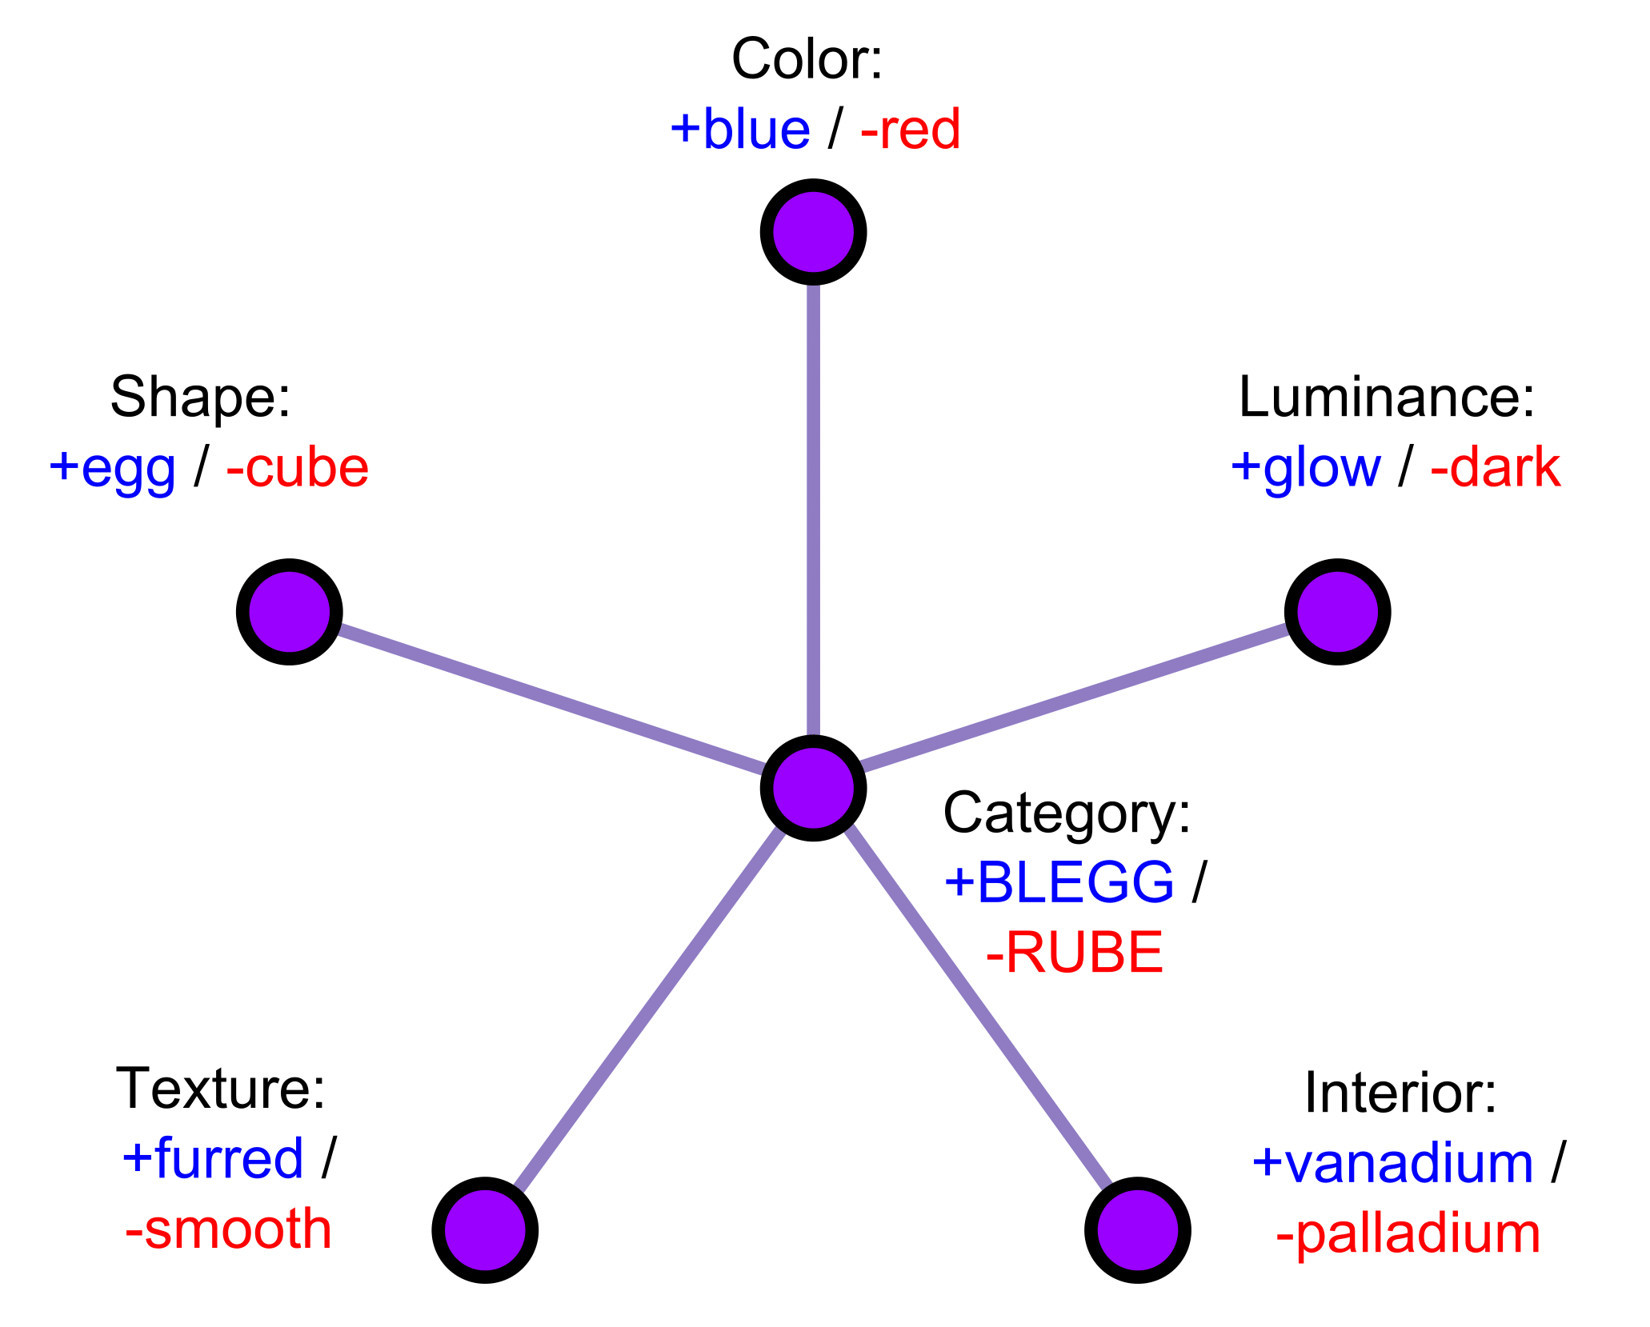
\includegraphics[scale=0.25]{Rationality20From20AI20to20Zombies2020Eliezer20Yudkowsky-img200.jpg}
 \newline
 Figure 177.1: Network 2
\par}


\bigskip

{
\ \ \ ~}

{
\ \ \ As a matter of fact, if you use the right kind of neural network
units, this ``neural network'' ends
up \textit{exactly, mathematically} equivalent to Naive Bayes. The
central unit just needs a logistic threshold---an S-curve
response---and the weights of the inputs just need to match the
logarithms of the likelihood ratios, et cetera. In fact,
it's a good guess that this is one of the reasons why
logistic response often works so well in neural networks---it lets the
algorithm sneak in a little Bayesian reasoning while the designers
aren't looking.}

{
\ \ \ Just because someone is presenting you with an algorithm that they
call a ``neural network'' with
buzzwords like ``scruffy'' and
``emergent'' plastered all over it,
disclaiming proudly that they have no idea how the learned network
works---well, don't assume that their little AI
algorithm \textit{really is} Beyond the Realms of Logic. For this
paradigm of adhockery, if it works, will turn out to have Bayesian
structure; it may even be exactly equivalent to an algorithm of the
sort called ``Bayesian.''}

{
\ \ \ Even if it doesn't \textit{look} Bayesian, on the
surface.}

{
\ \ \ And then you just \textit{know} that the Bayesians are going to
start explaining exactly how the algorithm works, what underlying
assumptions it reflects, which environmental regularities it exploits,
where it works and where it fails, and even attaching understandable
meanings to the learned network weights.}

{
\ \ \ Disappointing, isn't it?}

{\centering
\ \ \ \ ~
\par}

{\centering
\ \ \ *
\par}

\mysection{Words as Mental Paintbrush Handles}

{
\ \ \ Suppose I tell you: ``It's the
strangest thing: The lamps in this hotel have triangular
lightbulbs.''}

{
\ \ \ You may or may not have visualized it---if you
haven't done it yet, do so now---what, in your
mind's eye, does a ``triangular
lightbulb'' look like?}

{
\ \ \ In your mind's eye, did the glass have sharp
edges, or smooth?}

{
\ \ \ When the phrase ``triangular
lightbulb'' first crossed my mind---no, the hotel
doesn't have them---then as best as my introspection
could determine, I first saw a pyramidal lightbulb with sharp edges,
then (almost immediately) the edges were smoothed, and then my mind
generated a loop of flourescent bulb in the shape of a smooth triangle
as an alternative.}

{
\ \ \ As far as I can tell, no deliberative/verbal thoughts were
involved---just wordless reflex flinch away from the imaginary mental
vision of sharp glass, which design problem was solved before I could
even think in words.}

{
\ \ \ Believe it or not, for some decades, there was a serious debate
about whether people \textit{really} had mental images in their
mind---an actual \textit{picture} of a chair somewhere---or if people
just naively \textit{thought} they had mental images (having been
misled by ``introspection,'' a very
bad forbidden activity), while actually just having a little
``chair'' label, like a LISP token,
active in their brain.}

{
\ \ \ I am trying hard not to say anything like ``How
spectacularly silly,'' because there is always the
hindsight effect to consider, but: how spectacularly silly.}

{
\ \ \ This academic paradigm, I think, was mostly a deranged legacy of
behaviorism, which denied the existence of thoughts in humans, and
sought to explain all human phenomena as
``reflex,'' including speech.
Behaviorism probably deserves its own write at some point, as it was a
perversion of rationalism; but this is not that write.}

{
\ \ \ ``You call it
`silly,''' you
inquire, ``but how do you \textit{know} that your
brain represents visual images? Is it merely that you can close your
eyes and see them?''}

{
\ \ \ This question \textit{used} to be harder to answer, back in the
day of the controversy. If you wanted to prove the existence of mental
imagery ``scientifically,'' rather
than just by introspection, you had to infer the existence of mental
imagery from experiments like this: Show subjects two objects and ask
them if one can be rotated into correspondence with the other. The
response time is linearly proportional to the angle of rotation
required. This is easy to explain if you are actually visualizing the
image and continuously rotating it at a constant speed, but hard to
explain if you are just checking propositional features of the image.}

{
\ \ \ Today we can actually neuroimage the little pictures in the visual
cortex. So, yes, your brain really does represent a detailed image of
what it sees or imagines. See Stephen Kosslyn's
\textit{Image and Brain: The Resolution of the Imagery
Debate.}\textsuperscript{1}}

{
\ \ \ Part of the reason people get in trouble with words, is that they
do not realize how much complexity lurks behind words.}

{
\ \ \ Can you visualize a ``green
dog''? Can you visualize a ``cheese
apple''?}

{
\ \ \ ``Apple'' isn't
just a sequence of two syllables or five letters.
That's a shadow. That's the tip of the
tiger's tail.}

{
\ \ \ Words, or rather the concepts behind them, are paintbrushes---you
can use them to draw images in your own mind. Literally draw, if you
employ concepts to make a picture in your visual cortex. And by the use
of shared labels, you can reach into someone else's
mind, and grasp their paintbrushes to draw pictures in \textit{their}
minds---sketch a little green dog in their visual cortex.}

{
\ \ \ But don't think that, because you send syllables
through the air, or letters through the Internet, it is the syllables
or the letters that draw pictures in the visual cortex. That takes some
complex instructions that wouldn't fit in the sequence
of letters. ``Apple'' is 5 bytes,
and drawing a picture of an apple from scratch would take more data
than that.}

{
\ \ \ ``Apple'' is merely the tag
attached to the true and wordless \textit{apple} concept, which can
paint a picture in your visual cortex, or collide with
``cheese,'' or recognize an apple
when you see one, or taste its archetype in apple pie, maybe even send
out the motor behavior for eating an apple .~.~.}

{
\ \ \ And it's not as simple as just calling up a
picture from memory. Or how would you be able to visualize combinations
like a ``triangular
lightbulb''---imposing triangleness on lightbulbs,
keeping the essence of both, even if you've never seen
such a thing in your life?}

{
\ \ \ Don't make the mistake the behaviorists made.
There's far more to speech than sound in air. The
labels are just pointers---``look in memory area
1387540.'' Sooner or later, when
you're handed a pointer, it comes time to dereference
it, and actually look in memory area 1387540.}

{
\ \ \ What does a word point to?}

{\centering
\ \ \ \ ~
\par}

{\centering
\ \ \ *
\par}


\bigskip

{
\ \ \ 1. Stephen M. Kosslyn, \textit{Image and Brain: The Resolution of
the Imagery Debate} (Cambridge, MA: MIT Press, 1994).}

\mysection{Variable Question Fallacies}

{
\ \ \ ALBERT: ``Every time I've
listened to a tree fall, it made a sound, so I'll guess
that other trees falling also make sounds. I don't
believe the world changes around when I'm not
looking.''}

{
\ \ \ BARRY: ``Wait a minute. If no one hears it, how
can it be a sound?''}

{
\ \ \ While writing the dialogue of Albert and Barry in their dispute
over whether a falling tree in a deserted forest makes a sound, I
sometimes found myself losing empathy with my characters. I would start
to lose the gut feel of why \textit{anyone} would ever argue like that,
even though I'd seen it happen many times.}

{
\ \ \ On these occasions, I would repeat to myself,
``Either the falling tree makes a sound, or it does
not!'' to restore my borrowed sense of indignation.}

{
\ \ \ (P or {\textlnot}P) is not always a reliable heuristic, if you
substitute arbitrary English sentences for P. ``This
sentence is false'' cannot be consistently viewed as
true or false. And then there's the old classic,
``Have you stopped beating your
wife?''}

{
\ \ \ Now if you are a mathematician, and one who believes in classical
(rather than intuitionistic) logic, there are ways to continue
insisting that (P or {\textlnot}P) is a theorem: for example, saying
that ``This sentence is false'' is
not a sentence.}

{
\ \ \ But such resolutions are subtle, which suffices to demonstrate a
need for subtlety. You cannot just bull ahead on every occasion with
``Either it does or it
doesn't!''}

{
\ \ \ So does the falling tree make a sound, or not, or .~.~. ?}

{
\ \ \ Surely, 2 + 2 = X or it does not? Well, maybe, \textit{if}
it's \textit{really} the same X, the same 2, and the
same + and = . If X evaluates to 5 on some occasions and 4 on another,
your indignation may be misplaced.}

{
\ \ \ To even begin claiming that (P or {\textlnot}P) ought to be a
necessary truth, the symbol P must stand for \textit{exactly} the same
thing in both halves of the dilemma. ``Either the fall
makes a sound, or not!''---but if Albert::sound is
not the same as Barry::sound, there is nothing paradoxical about the
tree making an Albert::sound but not a Barry::sound.}

{
\ \ \ (The :: idiom is something I picked up in my C++ days for avoiding
namespace collisions. If you've got two different
packages that define a class Sound, you can write Package1::Sound to
specify which Sound you mean. The idiom is not widely known, I think;
which is a pity, because I often wish I could use it in writing.)}

{
\ \ \ The variability may be subtle: Albert and Barry may carefully
verify that it is the same tree, in the same forest, and the same
occasion of falling, just to ensure that they really do have a
substantive disagreement about exactly the same event. And then forget
to check that they are matching this event against exactly the same
concept.}

{
\ \ \ Think about the grocery store that you visit most often: Is it on
the left side of the street, or the right? But of course there is no
``\textit{the} left side'' of the
street, only \textit{your} left side, as you travel along it from some
particular direction. Many of the words we use are really functions of
implicit variables supplied by context.}

{
\ \ \ It's actually one heck of a pain, requiring one
heck of a lot of work, to handle this kind of problem in an Artificial
Intelligence program intended to parse language---the phenomenon going
by the name of ``speaker deixis.''}

{
\ \ \ ``Martin told Bob the building was on his
left.'' But
``left'' is a function-word that
evaluates with a speaker-dependent variable invisibly grabbed from the
surrounding context. Whose ``left''
is meant, Bob's or Martin's?}

{
\ \ \ The variables in a variable question fallacy often
aren't neatly labeled---it's not as
simple as ``Say, do you think Z + 2 equals
6?''}

{
\ \ \ If a namespace collision introduces two different concepts that
look like ``the same concept''
because they have the same name---or a map compression introduces two
different events that look like the same event because they
don't have separate mental files---or the same function
evaluates in different contexts---then reality itself becomes protean,
changeable. At least that's what the algorithm feels
like from inside. Your mind's eye sees the map, not the
territory directly.}

{
\ \ \ If you have a question with a hidden variable, that evaluates to
different expressions in different contexts, it \textit{feels like}
reality itself is unstable---what your mind's eye sees,
shifts around depending on where it looks.}

{
\ \ \ This often confuses undergraduates (and postmodernist professors)
who discover a sentence with more than one interpretation; they think
they have discovered an unstable portion of reality.}

{
\ \ \ ``Oh my gosh! `The Sun goes around
the Earth' is true for Hunga Huntergatherer, but for
Amara Astronomer, `The Sun goes around the
Earth' is false! There is no fixed
truth!'' The deconstruction of this sophomoric
nitwittery is left as an exercise to the reader.}

{
\ \ \ And yet, even I initially found myself writing
``If X is 5 on some occasions and 4 on another, the
sentence `2 + 2 = X' may have no fixed
truth-value.'' There is not \textit{one} sentence
with a \textit{variable} truth-value. ``2 + 2 =
X'' \textit{has no} truth-value. It is not a
\textit{proposition}, not yet, not as mathematicians define
proposition-ness, any more than ``2 + 2
='' is a proposition, or ``Fred
jumped over the'' is a grammatical sentence.}

{
\ \ \ But this fallacy tends to sneak in, even when you allegedly know
better, because, well, that's how the algorithm feels
from inside.}

{\centering
\ \ \ \ ~
\par}

{\centering
\ \ \ *
\par}

\mysection{37 Ways That Words Can Be Wrong}

{
\ \ \ Some reader is bound to declare that a better title for this essay
would be ``37 Ways That You Can Use Words
Unwisely,'' or ``37 Ways That
Suboptimal Use Of Categories Can Have Negative Side Effects On Your
Cognition.'' }

{
\ \ \ But one of the primary lessons of this gigantic list is that
saying ``There's no way my choice of X
can be `wrong''' is
nearly always an error in practice, whatever the theory. You can always
be wrong. Even when it's theoretically impossible to be
wrong, you can still be wrong. There is never a Get Out of Jail Free
card for anything you do. That's life.}

{
\ \ \ Besides, I can define the word
``wrong'' to mean anything I
like---it's not like a word can be \textit{wrong.}}

{
\ \ \ Personally, I think it quite justified to use the word
``wrong'' when:}

{
\ \ \ \textit{A word fails to connect to reality in the first place.} Is
Socrates a framster? Yes or no? (The Parable of the Dagger)}

{
\ \ \ \textit{Your argument, if it worked, could coerce reality to go a
different way by choosing a different word definition.} Socrates is a
human, and humans, by definition, are mortal. So if you defined humans
to not be mortal, would Socrates live forever? (The Parable of
Hemlock)}

{
\ \ \ \textit{You try to establish any sort of empirical proposition as
being true ``by definition.''}
Socrates is a human, and humans, by definition, are mortal. So is it a
\textit{logical truth} if we empirically predict that Socrates should
keel over if he drinks hemlock? It seems like there are logically
possible, non-self-contradictory worlds where Socrates
doesn't keel over---where he's immune
to hemlock by a quirk of biochemistry, say. Logical truths are true in
all possible worlds, and so never tell you \textit{which} possible
world you live in---and anything you can establish
``by definition'' is a logical
truth. (The Parable of Hemlock)}

{
\ \ \ \textit{You unconsciously slap the conventional label on
something, without actually using the verbal definition you just gave.}
You know perfectly well that Bob is
``human,'' even though, by your
definition, you can never call Bob
``human'' without first observing
him to be mortal. (The Parable of Hemlock)}

{
\ \ \ \textit{The act of labeling something with a word disguises a
challengable inductive inference you are making.} If the last 11
egg-shaped objects drawn have been blue, and the last 8 cubes drawn
have been red, it is a matter of induction to say this rule will hold
in the future. But if you call the blue eggs
``bleggs'' and the red cubes
``rubes,'' you may reach into the
barrel, feel an egg shape, and think ``Oh, a
blegg.'' (Words as Hidden Inferences)}

{
\ \ \ \textit{You try to define a word using words, in turn defined with
ever-more-abstract words, without being able to point to an example.}
``What is red?''
``Red is a color.''
``What's a color?''
``It's a property of a
thing.'' ``What's a
thing? What's a property?'' It never
occurs to you to point to a stop sign and an apple. (Extensions and
Intensions)}

{
\ \ \ \textit{The extension doesn't match the
intension.} We aren't consciously aware of our
identification of a red light in the sky as
``Mars,'' which will probably happen
regardless of your attempt to define
``Mars'' as ``The
God of War.'' (Extensions and Intensions)}

{
\ \ \ \textit{Your verbal definition doesn't capture
more than a tiny fraction of the category's shared
characteristics, but you try to reason as if it does.} When the
philosophers of Plato's Academy claimed that the best
definition of a human was a ``featherless
biped,'' Diogenes the Cynic is said to have exhibited
a plucked chicken and declared ``Here is
Plato's Man.'' The Platonists
promptly changed their definition to ``a featherless
biped with broad nails.'' (Similarity Clusters)}

{
\ \ \ \textit{You try to treat category membership as all-or-nothing,
ignoring the existence of more and less typical subclusters.} Ducks and
penguins are less typical birds than robins and pigeons. Interestingly,
a between-groups experiment showed that subjects thought a disease was
more likely to spread from robins to ducks on an island, than from
ducks to robins. (Typicality and Asymmetrical Similarity)}

{
\ \ \ \textit{A verbal definition works well enough in practice to point
out the intended cluster of similar things, but you nitpick
exceptions.} Not every human has ten fingers, or wears clothes, or uses
language; but if you look for an empirical cluster of things which
share these characteristics, you'll get enough
information that the occasional nine-fingered human
won't fool you. (The Cluster Structure of Thingspace)}

{
\ \ \ \textit{You ask whether something
``is'' or ``is
not'' a category member but can't
name the question you really want answered.} What is a
``man''? Is Barney the Baby Boy a
``man''? The
``correct'' answer may depend
considerably on whether the query you \textit{really} want answered is
``Would hemlock be a good thing to feed
Barney?'' or ``Will Barney make a
good husband?'' (Disguised Queries)}

{
\ \ \ \textit{You treat intuitively perceived hierarchical categories
like the only correct way to parse the world, without realizing that
other forms of statistical inference are possible even though your
brain doesn't use them.} It's much
easier \textit{for a human} to notice whether an object is a
``blegg'' or
``rube''; than \textit{for a human}
to notice that red objects never glow in the dark, but red furred
objects have all the other characteristics of bleggs. Other statistical
algorithms work differently. (Neural Categories)}

{
\ \ \ \textit{You talk about categories as if they are manna fallen from
the Platonic Realm, rather than inferences implemented in a real
brain.} The ancient philosophers said ``Socrates is a
man,'' not, ``My brain perceptually
classifies Socrates as a match against the
`human' concept.''
(How An Algorithm Feels From Inside)}

{
\ \ \ \textit{You argue about a category membership even after screening
off all questions that could possibly depend on a category-based
inference.} After you observe that an object is blue, egg-shaped,
furred, flexible, opaque, luminescent, and palladium-containing,
what's \textit{left} to ask by arguing,
``Is it a blegg?'' But if your
brain's categorizing neural network contains a
(metaphorical) central unit corresponding to the inference of
blegg-ness, it may still \textit{feel} like there's a
leftover question. (How An Algorithm Feels From Inside)}

{
\ \ \ \textit{You allow an argument to slide into being about
definitions, even though it isn't what you originally
wanted to argue about.} If, before a dispute started about whether a
tree falling in a deserted forest makes a
``sound,'' you asked the two
soon-to-be arguers whether they thought a
``sound'' should be defined as
``acoustic vibrations'' or
``auditory experiences,''
they'd probably tell you to flip a coin. Only after the
argument starts does the definition of a word become politically
charged. (Disputing Definitions)}

{
\ \ \ \textit{You think a word has a meaning, as a property of the word
itself; rather than there being a label that your brain associates to a
particular concept.} When someone shouts ``Yikes! A
tiger!,'' evolution would not favor an organism that
thinks, ``Hm .~.~. I have just heard the syllables
`Tie' and
`Grr' which my fellow tribemembers
associate with their internal analogues of my own \textit{tiger}
concept and which \textit{aiiieeee} CRUNCH CRUNCH
GULP.'' So the brain takes a shortcut, and it seems
that the meaning of tigerness is a property of the label itself. People
argue about the \textit{correct meaning} of a label like
``sound.'' (Feel the Meaning)}

{
\ \ \ \textit{You argue over the meanings of a word, even after all
sides understand perfectly well what the other sides are trying to
say.} The human ability to associate labels to concepts is a tool for
communication. When people \textit{want} to communicate,
we're hard to stop; if we have no common language,
we'll draw pictures in sand. When you each understand
what is in the other's mind, you are \textit{done}.
(The Argument From Common Usage)}

{
\ \ \ \textit{You pull out a dictionary in the middle of an empirical or
moral argument.} Dictionary editors are historians of usage, not
legislators of language. If the common definition contains a
problem---if ``Mars'' is defined as
the God of War, or a ``dolphin'' is
defined as a kind of fish, or
``Negroes'' are defined as a
separate category from humans, the dictionary will reflect the standard
mistake. (The Argument From Common Usage)}

{
\ \ \ \textit{You pull out a dictionary in the middle of any argument
ever.} Seriously, what the heck makes you think that dictionary editors
are an authority on whether
``atheism'' is a
``religion'' or whatever? If you
have any substantive issue whatsoever at stake, do you really think
dictionary editors have access to ultimate wisdom that settles the
argument? (The Argument From Common Usage)}

{
\ \ \ \textit{You defy common usage without a reason, making it
gratuitously hard for others to understand you.} Fast stand up
plutonium, with bagels without handle. (The Argument From Common
Usage)}

{
\ \ \ \textit{You use complex renamings to create the illusion of
inference.} Is a ``human'' defined
as a ``mortal featherless biped''?
Then write: ``All [mortal featherless bipeds] are
mortal; Socrates is a [mortal featherless biped]; therefore, Socrates
is mortal.'' Looks less impressive that way,
doesn't it? (Empty Labels)}

{
\ \ \ \textit{You get into arguments that you could avoid if you just
didn't use the word.} If Albert and Barry
aren't allowed to use the word
``sound,'' then Albert will have to
say ``A tree falling in a deserted forest generates
acoustic vibrations,'' and Barry will say
``A tree falling in a deserted forest generates no
auditory experiences.'' When a word poses a problem,
the simplest solution is to eliminate the word and its synonyms. (Taboo
Your Words)}

{
\ \ \ \textit{The existence of a neat little word prevents you from
seeing the details of the thing you're trying to think
about.} What actually goes on in schools once you stop calling it
``education''?
What's a degree, once you stop calling it a
``degree''? If a coin lands
``heads,'' what's
its radial orientation? What is
``truth,'' if you
can't say
``accurate'' or
``correct'' or
``represent'' or
``reflect'' or
``semantic'' or
``believe'' or
``knowledge'' or
``map'' or
``real'' or any other simple term?
(Replace the Symbol with the Substance)}

{
\ \ \ \textit{You have only one word, but there are two or more
different things-in-reality, so that all the facts about them get
dumped into a single undifferentiated mental bucket.}
It's part of a detective's ordinary
work to observe that Carol wore red last night, or that she has black
hair; and it's part of a detective's
ordinary work to wonder if maybe Carol dyes her hair. But it takes a
subtler detective to wonder if there are two Carols, so that the Carol
who wore red is not the same as the Carol who had black hair.
(Fallacies of Compression)}

{
\ \ \ \textit{You see patterns where none exist, harvesting other
characteristics from your }\textit{definitions even when there is no
similarity along that dimension.} In Japan, it is thought that people
of blood type A are earnest and creative, blood type Bs are wild and
cheerful, blood type Os are agreeable and sociable, and blood type ABs
are cool and controlled. (Categorizing Has Consequences)}

{
\ \ \ \textit{You try to sneak in the connotations of a word, by arguing
from a definition that doesn't include the
connotations.} A ``wiggin'' is
defined in the dictionary as a person with green eyes and black hair.
The word ``wiggin'' also carries the
connotation of someone who commits crimes and launches cute baby
squirrels, but that part isn't in the dictionary. So
you point to someone and say: ``Green eyes? Black
hair? See, told you he's a wiggin! Watch, next
he's going to steal the silverware.''
(Sneaking in Connotations)}

{
\ \ \ \textit{You claim ``X, by definition, is a
Y!'' On such occasions you're almost
certainly trying to sneak in a connotation of Y that
wasn't in your given definition.} You define
``human'' as a
``featherless biped,'' and point to
Socrates and say, ``No feathers---two legs---he must
be human!'' But what you \textit{really} care about
is something else, like mortality. If what was in dispute was
Socrates's number of legs, the other fellow would just
reply, ``Whaddaya mean, Socrates's got
two legs? That's what we're arguing
about in the first place!'' (Arguing
``By Definition'')}

{
\ \ \ \textit{You claim ``Ps, by definition, are
Qs!''} If you see Socrates out in the field with some
biologists, gathering herbs that might confer resistance to hemlock,
there's no point in arguing ``Men, by
definition, are mortal!'' The main time you feel the
need to tighten the vise by insisting that something is true
``by definition'' is when
there's other information that calls the default
inference into doubt. (Arguing ``By
Definition'')}

{
\ \ \ \textit{You try to establish membership in an empirical cluster
``by definition.''} You
wouldn't feel the need to say,
``Hinduism, \textit{by definition,} is a
religion!'' because, well, of course Hinduism is a
religion. It's not just a religion
``by definition,''
it's, like, an \textit{actual} religion. Atheism does
not resemble the central members of the
``religion'' cluster, so if it
wasn't for the fact that atheism is a religion
\textit{by definition,} you might go around thinking that atheism
\textit{wasn't} a religion. That's why
you've got to crush all opposition by pointing out that
``Atheism is a religion'' is true
\textit{by definition,} because it isn't true any other
way. (Arguing ``By Definition'')}

{
\ \ \ \textit{Your definition draws a boundary around things that
don't really belong together.} You can claim, if you
like, that you are \textit{defining} the word
``fish'' to refer to salmon,
guppies, sharks, dolphins, and trout, but not jellyfish or algae. You
can claim, if you like, that this is merely a list, and there is no way
a list can be ``wrong.'' Or you can
stop playing games and admit that you made a mistake and that dolphins
don't belong on the fish list. (Where to Draw the
Boundary?)}

{
\ \ \ \textit{You use a short word for something that you
won't need to describe often, or a long word for
something you'll need to describe often. This can
result in inefficient thinking, or even misapplications of
Occam's Razor, if your mind thinks that short sentences
sound ``simpler.''} Which sounds
more plausible, ``God did a
miracle'' or ``A supernatural
universe-creating entity temporarily suspended the laws of
physics''? (Entropy, and Short Codes)}

{
\ \ \ \textit{You draw your boundary around a volume of space where
there is no greater-than-usual density, meaning that the associated
word does not correspond to any performable Bayesian inferences.} Since
green-eyed people are not more likely to have black hair, or vice
versa, and they don't share any other characteristics
in common, why have a word for
``wiggin''? (Mutual Information, and
Density in Thingspace)}

{
\ \ \ \textit{You draw an unsimple boundary without any reason to do
so.} The act of defining a word to refer to all humans, except black
people, seems kind of suspicious. If you don't present
reasons to draw that particular boundary, trying to create an
``arbitrary'' word in that location
is like a detective saying: ``Well, I
haven't the slightest shred of support one way or the
other for who could've murdered those orphans .~.~. but
have we considered John Q. Wiffleheim as a suspect?''
(Superexponential Conceptspace, and Simple Words)}

{
\ \ \ \textit{You use categorization to make inferences about properties
that don't have the appropriate empirical structure,
namely, conditional independence given knowledge of the class, to be
well-approximated by Naive Bayes.} No way am I trying to summarize this
one. Just read the essay. (Conditional Independence, and Naive Bayes)}

{
\ \ \ \textit{You think that words are like tiny little LISP symbols in
your mind, rather than words being labels that act as handles to direct
complex mental paintbrushes that can paint detailed pictures in your
sensory workspace.} Visualize a ``triangular
lightbulb.'' What did you see? (Words as Mental
Paintbrush Handles)}

{
\ \ \ \textit{You use a word that has different meanings in different
places as though it meant the same thing on each occasion, possibly
creating the illusion of something protean and shifting.}
``Martin told Bob the building was on his
left.'' But
``left'' is a function-word that
evaluates with a speaker-dependent variable grabbed from the
surrounding context. Whose ``left''
is meant, Bob's or Martin's? (Variable
Question Fallacies)}

{
\ \ \ \textit{You think that definitions can't be
``wrong,'' or that
``I can define a word any way I
like!''} This kind of attitude teaches you to
indignantly defend your past actions, instead of paying attention to
their consequences, or fessing up to your mistakes. (37 Ways That
Suboptimal Use Of Categories Can Have Negative Side Effects On Your
Cognition)}

{
\ \ \ Everything you do in the mind has an effect, and your brain races
ahead unconsciously without your supervision.}

{
\ \ \ Saying ``Words are arbitrary; I can define a word
any way I like'' makes around as much sense as
driving a car over thin ice with the accelerator floored and saying,
``Looking at this steering wheel, I
can't see why one radial angle is special---so I can
turn the steering wheel any way I like.''}

{
\ \ \ If you're trying to go anywhere, or even just
trying to \textit{survive}, you had better start paying attention to
the three or six dozen optimality criteria that control how you use
words, definitions, categories, classes, boundaries, labels, and
concepts.}

{\centering
\ \ \ \ ~
\par}

{\centering
\ \ \ *
\par}

\mysectionnn{Interlude An Intuitive Explanation of Bayes's Theorem}

{
\ \textit{\ \ \ }\textbf{\textit{Editor's
Note:}}\textit{ This is an abridgement of the
}\textit{original}\textit{ version of this essay, which contained many
interactive elements.}}

{
\textit{\ \ \ ~}}

{
\textit{\ }\ \ \ Your friends and colleagues are talking about something
called ``Bayes's
Theorem'' or
``Bayes's Rule,'' or
something called Bayesian reasoning. They sound really enthusiastic
about it, too, so you google and find a web page about
Bayes's Theorem and .~.~.}

{
\ \ \ It's this equation. That's all.
Just one equation. The page you found gives a definition of it, but it
doesn't say what it is, or why it's
useful, or why your friends would be interested in it. It looks like
this random statistics thing.}

{
\ \ \ Why does a mathematical concept generate this strange enthusiasm
in its students? What is the so-called Bayesian Revolution now sweeping
through the sciences, which claims to subsume even the experimental
method itself as a special case? What is the secret that the adherents
of Bayes know? What is the light that they have seen?}

{
\ \ \ Soon you will know. Soon you will be one of us.}

{
\ \ \ While there are a few existing online explanations of
Bayes's Theorem, my experience with trying to introduce
people to Bayesian reasoning is that the existing online explanations
are too abstract. Bayesian reasoning is very \textit{counterintuitive}.
People do not employ Bayesian reasoning intuitively, find it very
difficult to learn Bayesian reasoning when tutored, and rapidly forget
Bayesian methods once the tutoring is over. This holds equally true for
novice students and highly trained professionals in a field. Bayesian
reasoning is apparently one of those things which, like quantum
mechanics or the Wason Selection Test, is inherently difficult for
humans to grasp with our built-in mental faculties.}

{
\ \ \ Or so they claim. Here you will find an attempt to offer an
\textit{intuitive} explanation of Bayesian reasoning---an
excruciatingly gentle introduction that invokes all the human ways of
grasping numbers, from natural frequencies to spatial visualization.
The intent is to convey, not abstract rules for manipulating numbers,
but what the numbers mean, and why the rules are what they are (and
cannot possibly be anything else). When you are finished reading this,
you will see Bayesian problems in your dreams.}

{
\ \ \ And let's begin.}

{
\ \ \ Here's a story problem about a situation that
doctors often encounter:}

{
\ \ \ 1\% of women at age forty who participate in routine screening
have breast cancer. 80\% of women with breast cancer will get positive
mammographies. 9.6\% of women without breast cancer will also get
positive mammographies. A woman in this age group had a positive
mammography in a routine screening. What is the probability that she
actually has breast cancer?}

{
\ \ \ What do you think the answer is? If you haven't
encountered this kind of problem before, please take a moment to come
up with your own answer before continuing.}

{
\ \ \ Next, suppose I told you that most doctors get the same wrong
answer on this problem---usually, only around 15\% of doctors get it
right. (``Really? 15\%? Is that a real number, or an
urban legend based on an Internet poll?''
It's a real number. See Casscells, Schoenberger, and
Graboys 1978;\textsuperscript{1} Eddy 1982;\textsuperscript{2}
Gigerenzer and Hoffrage 1995;\textsuperscript{3} and many other
studies. It's a surprising result which is easy to
replicate, so it's been extensively replicated.)}

{
\ \ \ On the story problem above, most doctors estimate the probability
to be between 70\% and 80\%, which is wildly incorrect.}

{
\ \ \ Here's an alternate version of the problem on
which doctors fare somewhat better:}

{
\ \ \ 10 out of 1,000 women at age forty who participate in routine
screening have breast cancer. 800 out of 1,000 women with breast cancer
will get positive mammographies. 96 out of 1,000 women without breast
cancer will also get positive mammographies. If 1,000 women in this age
group undergo a routine screening, about what fraction of women with
positive mammographies will actually have breast cancer?}

{
\ \ \ And finally, here's the problem on which doctors
fare best of all, with 46\%---nearly half---arriving at the correct
answer:}

{
\ \ \ 100 out of 10,000 women at age forty who participate in routine
screening have breast cancer. 80 of every 100 women with breast cancer
will get a positive mammography. 950 out of 9,900 women without breast
cancer will also get a positive mammography. If 10,000 women in this
age group undergo a routine screening, about what fraction of women
with positive mammographies will actually have breast cancer?}

{
\ \ \ The correct answer is 7.8\%, obtained as follows: Out of 10,000
women, 100 have breast cancer; 80 of those 100 have positive
mammographies. From the same 10,000 women, 9,900 will not have breast
cancer and of those 9,900 women, 950 will also get positive
mammographies. This makes the total number of women with positive
mammographies 950 + 80 or 1,030. Of those 1,030 women with positive
mammographies, 80 will have cancer. Expressed as a proportion, this is
80/1,030 or 0.07767 or 7.8\%.}

{
\ \ \ To put it another way, before the mammography screening, the
10,000 women can be divided into two groups:}

{
\ \ \ Group 1: 100 women \textit{with} breast cancer.}

{
\ \ \ Group 2: 9,900 women \textit{without} breast cancer.}

{
\ \ \ Summing these two groups gives a total of 10,000 patients,
confirming that none have been lost in the math. After the mammography,
the women can be divided into four groups:}

{
\ \ \ Group A: 80 women \textit{with} breast cancer and a
\textit{positive} mammography.}

{
\ \ \ Group B: 20 women \textit{with} breast cancer and a
\textit{negative} mammography.}

{
\ \ \ Group C: 950 women \textit{without} breast cancer and a
\textit{positive} mammography.}

{
\ \ \ Group D: 8,950 women \textit{without} breast cancer and a
\textit{negative} mammography.}

{
\ \ \ The sum of groups A and B, the groups with breast cancer,
corresponds to group 1; and the sum of groups C and D, the groups
without breast cancer, corresponds to group 2. If you administer a
mammography to 10,000 patients, then out of the 1,030 with positive
mammographies, eighty of those positive-mammography patients will have
cancer. This is the correct answer, the answer a doctor should give a
positive-mammography patient if she asks about the chance she has
breast cancer; if thirteen patients ask this question, roughly one out
of those thirteen will have cancer.}

{
\ \ \ The most common mistake is to ignore the original fraction of
women with breast cancer, and the fraction of women without breast
cancer who receive false positives, and focus only on the fraction of
women with breast cancer who get positive results. For example, the
vast majority of doctors in these studies seem to have thought that if
around 80\% of women with breast cancer have positive mammographies,
then the probability of a women with a positive mammography having
breast cancer must be around 80\%.}

{
\ \ \ Figuring out the final answer always requires \textit{all three}
pieces of information---the percentage of women with breast cancer, the
percentage of women without breast cancer who receive false positives,
and the percentage of women with breast cancer who receive (correct)
positives.}

{
\ \ \ The original proportion of patients with breast cancer is known as
the \textit{prior probability}. The chance that a patient with breast
cancer gets a positive mammography, and the chance that a patient
without breast cancer gets a positive mammography, are known as the two
\textit{conditional probabilities}. Collectively, this initial
information is known as \textit{the priors}. The final answer---the
estimated probability that a patient has breast cancer, given that we
know she has a positive result on her mammography---is known as the
\textit{revised probability} or the \textit{posterior probability}.
What we've just seen is that the posterior probability
depends in part on the prior probability.}

{
\ \ \ To see that the final answer always depends on the original
fraction of women with breast cancer, consider an alternate universe in
which only one woman out of a million has breast cancer. Even if
mammography in this world detects breast cancer in 8 out of 10 cases,
while returning a false positive on a woman without breast cancer in
only 1 out of 10 cases, there will still be a hundred thousand false
positives for every real case of cancer detected. The original
probability that a woman has cancer is so extremely low that, although
a positive result on the mammography does \textit{increase} the
estimated probability, the probability isn't increased
to certainty or even ``a noticeable
chance''; the probability goes from 1:1,000,000 to
1:100,000.}

{
\ \ \ What this demonstrates is that the mammography result
doesn't \textit{replace} your old information about the
patient's chance of having cancer; the mammography
\textit{slides} the estimated probability in the direction of the
result. A positive result slides the original probability upward; a
negative result slides the probability downward. For example, in the
original problem where 1\% of the women have cancer, 80\% of women with
cancer get positive mammographies, and 9.6\% of women without cancer
get positive mammographies, a positive result on the mammography
\textit{slides} the 1\% chance upward to 7.8\%.}

{
\ \ \ Most people encountering problems of this type for the first time
carry out the mental operation of \textit{replacing} the original 1\%
probability with the 80\% probability that a woman with cancer gets a
positive mammography. It may seem like a good idea, but it just
doesn't work. ``The probability that a
woman with a positive mammography has breast cancer''
is not at all the same thing as ``the probability that
a woman with breast cancer has a positive
mammography''; they are as unlike as apples and
cheese.}

{
\ \ \ \textbf{Q. Why did the Bayesian reasoner cross the road?}}

{
\ \ \ A. You need more information to answer this question.}

{
\ \ \ Suppose that a barrel contains many small plastic eggs. Some eggs
are painted red and some are painted blue. 40\% of the eggs in the bin
contain pearls, and 60\% contain nothing. 30\% of eggs containing
pearls are painted blue, and 10\% of eggs containing nothing are
painted blue. What is the probability that a blue egg contains a pearl?
For this example the arithmetic is simple enough that you may be able
to do it in your head, and I would suggest trying to do so.}

{
\ \ \ A more compact way of specifying the problem:}

{\centering
\ \ \ P(pearl) = 40\%
\par}


\bigskip

{\centering
\ \ \ P(blue{\textbar}pearl) = 30\%
\par}


\bigskip

{\centering
\ \ \ P(blue{\textbar}{\textlnot}pearl) = 10\%
\par}


\bigskip

{\centering
\ \ \ P(pearl{\textbar}blue) = ?
\par}


\bigskip

{
\ \ \ The symbol ``{\textlnot}'' is
shorthand for ``not,'' so
{\textlnot}pearl reads ``not
pearl.''}

{
\ \ \ The notation P(blue{\textbar}pearl) is shorthand for
``the probability of blue given
pearl'' or ``the probability that an
egg is painted blue, given that the egg contains a
pearl.'' The item on the right side is what you
\textit{already know} or the \textit{premise}, and the item on the left
side is the \textit{implication} or \textit{conclusion}. If we have
P(blue{\textbar}pearl) = 30\%, and we \textit{already know} that some
egg contains a pearl, then we can \textit{conclude} there is a 30\%
chance that the egg is painted blue. Thus, the final fact
we're looking for---``the chance that
a blue egg contains a pearl'' or
``the probability that an egg contains a pearl, if we
know the egg is painted blue''---reads
P(pearl{\textbar}blue).}

{
\ \ \ 40\% of the eggs contain pearls, and 60\% of the eggs contain
nothing. 30\% of the eggs containing pearls are painted blue, so 12\%
of the eggs altogether contain pearls and are painted blue. 10\% of the
eggs containing nothing are painted blue, so altogether 6\% of the eggs
contain nothing and are painted blue. A total of 18\% of the eggs are
painted blue, and a total of 12\% of the eggs are painted blue and
contain pearls, so the chance a blue egg contains a pearl is 12/18 or
2/3 or around 67\%.}

{
\ \ \ As before, we can see the necessity of all three pieces of
information by considering extreme cases. In a (large) barrel in which
only one egg out of a thousand contains a pearl, knowing that an egg is
painted blue slides the probability from 0.1\% to 0.3\% (instead of
sliding the probability from 40\% to 67\%). Similarly, if 999 out of
1,000 eggs contain pearls, knowing that an egg is blue slides the
probability from 99.9\% to 99.966\%; the probability that the egg does
\textit{not} contain a pearl goes from 1/1,000 to around 1/3,000.}

{
\ \ \ On the pearl-egg problem, most respondents unfamiliar with
Bayesian reasoning would probably respond that the probability a blue
egg contains a pearl is 30\%, or perhaps 20\% (the 30\% chance of a
true positive minus the 10\% chance of a false positive). Even if this
mental operation seems like a good idea at the time, it makes no sense
in terms of the question asked. It's like the
experiment in which you ask a second-grader: ``If
eighteen people get on a bus, and then seven more people get on the
bus, how old is the bus driver?'' Many second-graders
will respond: ``Twenty-five.'' They
understand when they're being prompted to carry out a
particular mental procedure, but they haven't quite
connected the procedure to reality. Similarly, to find the probability
that a woman with a positive mammography has breast cancer, it makes no
sense whatsoever to \textit{replace} the original probability that the
woman has cancer with the probability that a woman with breast cancer
gets a positive mammography. Neither can you subtract the probability
of a false positive from the probability of the true positive. These
operations are as wildly irrelevant as adding the number of people on
the bus to find the age of the bus driver.}

{
\ \ \ A study by Gigerenzer and Hoffrage in 1995 showed that some ways
of phrasing story problems are much more evocative of correct Bayesian
reasoning.\textsuperscript{4} The \textit{least} evocative phrasing
used probabilities. A slightly more evocative phrasing used frequencies
instead of probabilities; the problem remained the same, but instead of
saying that 1\% of women had breast cancer, one would say that 1 out of
100 women had breast cancer, that 80 out of 100 women with breast
cancer would get a positive mammography, and so on. Why did a higher
proportion of subjects display Bayesian reasoning on this problem?
Probably because saying ``1 out of 100
women'' encourages you to concretely visualize X
women with cancer, leading you to visualize X women with cancer and a
positive mammography, etc.}

{
\ \ \ The most effective presentation found so far is
what's known as \textit{natural frequencies}{}---saying
that 40 out of 100 eggs contain pearls, 12 out of 40 eggs containing
pearls are painted blue, and 6 out of 60 eggs containing nothing are
painted blue. A \textit{natural frequencies} presentation is one in
which the information about the prior probability is included in
presenting the conditional probabilities. If you were just learning
about the eggs' conditional probabilities through
natural experimentation, you would---in the course of cracking open a
hundred eggs---crack open around 40 eggs containing pearls, of which 12
eggs would be painted blue, while cracking open 60 eggs containing
nothing, of which about 6 would be painted blue. In the course of
learning the conditional probabilities, you'd see
examples of blue eggs containing pearls about twice as often as you saw
examples of blue eggs containing nothing.}

{
\ \ \ Unfortunately, while natural frequencies are a step in the right
direction, it probably won't be enough. When problems
are presented in natural frequencies, the proportion of people using
Bayesian reasoning rises to around half. A big improvement, but not big
enough when you're talking about real doctors and real
patients.}

{
\ \ \ \textbf{Q. How can I find the priors for a problem?}\newline
 A. Many commonly used priors are listed in the \textit{Handbook of
Chemistry and Physics}.}

{
\ \ \ \textbf{Q. Where do priors }\textbf{\textit{originally}}\textbf{
come from?}\newline
 A. Never ask that question.}

{
\ \ \ \textbf{Q. Uh huh. Then where do scientists get their
priors?}\newline
 A. Priors for scientific problems are established by annual vote of the
AAAS. In recent years the vote has become fractious and controversial,
with widespread acrimony, factional polarization, and several outright
assassinations. This may be a front for infighting within the Bayes
Council, or it may be that the disputants have too much spare time. No
one is really sure.}

{
\ \ \ \textbf{Q. I see. And where does everyone else get their
priors?}\newline
 A. They download their priors from Kazaa.}

{
\ \ \ \textbf{Q. What if the priors I want aren't
available on Kazaa?}\newline
 A. There's a small, cluttered antique shop in a back
alley of San Francisco's Chinatown.
\textit{Don't ask about the bronze rat.}}

{
\ \ \ Actually, priors are true or false just like the final
answer---they reflect reality and can be judged by comparing them
against reality. For example, if you think that 920 out of 10,000 women
in a sample have breast cancer, and the actual number is 100 out of
10,000, then your priors are wrong. For our particular problem, the
priors might have been established by three studies---a study on the
case histories of women with breast cancer to see how many of them
tested positive on a mammography, a study on women without breast
cancer to see how many of them test positive on a mammography, and an
epidemiological study on the prevalence of breast cancer in some
specific demographic.}

{
\ \ \ The probability P(A,B) is the same as P(B,A), but P(A{\textbar}B)
is not the same thing as P(B{\textbar}A), and P(A,B) is completely
different from P(A{\textbar}B). It's a common confusion
to mix up some or all of these quantities.}

{
\ \ \ To get acquainted with all the relationships between them,
we'll play ``follow the degrees of
freedom.'' For example, the two quantities P(cancer)
and P({\textlnot}cancer) have one degree of freedom between them,
because of the general law P(A) + P({\textlnot}A) = 1. If you know that
P({\textlnot}cancer) = 0.99, you can obtain P(cancer) = 1 -
P({\textlnot}cancer) = 0.01.}

{
\ \ \ The quantities P(positive{\textbar}cancer) and
P({\textlnot}positive{\textbar}cancer) also have only one degree of
freedom between them; either a woman with breast cancer gets a positive
mammography or she doesn't. On the other hand,
P(positive{\textbar}cancer) and P(positive{\textbar}{\textlnot}cancer)
have \textit{two} degrees of freedom. You can have a mammography test
that returns positive for 80\% of cancer patients and 9.6\% of healthy
patients, or that returns positive for 70\% of cancer patients and 2\%
of healthy patients, or even a health test that returns
``positive'' for 30\% of cancer
patients and 92\% of healthy patients. The two quantities, the output
of the mammography test for cancer patients and the output of the
mammography test for healthy patients, are in mathematical terms
independent; one cannot be obtained from the other in any way, and so
they have two degrees of freedom between them.}

{
\ \ \ What about P(positive, cancer), P(positive{\textbar}cancer), and
P(cancer)? Here we have three quantities; how many degrees of freedom
are there? In this case the equation that must hold is}

{\centering
\ \ \ P(positive, cancer) = P(positive{\textbar}cancer) {\texttimes}
P(cancer).
\par}


\bigskip

{
\ \ \ This equality reduces the degrees of freedom by one. If we know
the fraction of patients with cancer, and the chance that a cancer
patient has a positive mammography, we can deduce the fraction of
patients who have breast cancer \textit{and} a positive mammography by
multiplying.}

{
\ \ \ Similarly, if we know the number of patients with breast cancer
and positive mammographies, and also the number of patients with breast
cancer, we can estimate the chance that a woman with breast cancer gets
a positive mammography by dividing: P(positive{\textbar}cancer) =
P(positive, cancer)$/$P(cancer). In fact, this is exactly how such
medical diagnostic tests are calibrated; you do a study on 8,520 women
with breast cancer and see that there are 6,816 (or thereabouts) women
with breast cancer and positive mammographies, then divide 6,816 by
8,520 to find that 80\% of women with breast cancer had positive
mammographies. (Incidentally, if you accidentally divide 8,520 by 6,816
instead of the other way around, your calculations will start doing
strange things, such as insisting that 125\% of women with breast
cancer and positive mammographies have breast cancer. This is a common
mistake in carrying out Bayesian arithmetic, in my experience.) And
finally, if you know P(positive, cancer) and
P(positive{\textbar}cancer), you can deduce how many cancer patients
there must have been originally. There are two degrees of freedom
shared out among the three quantities; if we know any two, we can
deduce the third.}

{
\ \ \ How about P(positive), P(positive, cancer), and
P(positive,{\textlnot}cancer)? Again there are only two degrees of
freedom among these three variables. The equation occupying the extra
degree of freedom is}

{\centering
\ \ \ P(positive) = P(positive, cancer) + P(positive,{\textlnot}cancer).
\par}


\bigskip

{
\ \ \ This is how P(positive) is computed to begin with; we figure out
the number of women with breast cancer who have positive mammographies,
and the number of women without breast cancer who have positive
mammographies, then add them together to get the total number of women
with positive mammographies. It would be very strange to go out and
conduct a study to determine the number of women with positive
mammographies---just that one number and nothing else---but in theory
you could do so. And if you then conducted another study and found the
number of those women who had positive mammographies \textit{and}
breast cancer, you would also know the number of women with positive
mammographies and \textit{no} breast cancer---either a woman with a
positive mammography has breast cancer or she doesn't.
In general, P(A,B) + P(A,{\textlnot}B) = P(A). Symmetrically, P(A,B) +
P({\textlnot}A,B) = P(B).}

{
\ \ \ What about P(positive, cancer), P(positive,{\textlnot}cancer),
P({\textlnot}positive, cancer), and
P({\textlnot}positive,{\textlnot}cancer)? You might at first be tempted
to think that there are only two degrees of freedom for these four
quantities---that you can, for example, get
P(positive,{\textlnot}cancer) by multiplying P(positive) {\texttimes}
P({\textlnot}cancer), and thus that all four quantities can be found
given only the two quantities P(positive) and P(cancer). This is not
the case! P(positive,{\textlnot}cancer) = P(positive) {\texttimes}
P({\textlnot}cancer) only if the two probabilities are
\textit{statistically independent}{}---if the chance that a woman has
breast cancer has no bearing on whether she has a positive mammography.
This amounts to requiring that the two conditional probabilities be
equal to each other---a requirement which would eliminate one degree of
freedom. If you remember that these four quantities are the groups A,
B, C, and D, you can look over those four groups and realize that, in
theory, you can put any number of people into the four groups. If you
start with a group of 80 women with breast cancer and positive
mammographies, there's no reason why you
can't add another group of 500 women with breast cancer
and negative mammographies, followed by a group of 3 women without
breast cancer and negative mammographies, and so on. So now it seems
like the four quantities have four degrees of freedom. And they would,
except that in expressing them as \textit{probabilities}, we need to
normalize them to \textit{fractions} of the complete group, which adds
the constraint that P(positive,
cancer)+P(positive,{\textlnot}cancer)+P({\textlnot}positive,
cancer)+P({\textlnot}positive,{\textlnot}cancer) = 1. This equation
takes up one degree of freedom, leaving three degrees of freedom among
the four quantities. If you specify the \textit{fractions} of women in
groups A, B, and D, you can deduce the fraction of women in group C.}

{
\ \ \ Given the four groups A, B, C, and D, it is very straightforward
to compute everything else:}

{\centering
\ \ \ P(cancer) = (A + B) / (A + B + C + D)
\par}


\bigskip

{\centering
\ \ \ P({\textlnot}positive{\textbar}cancer) = B / (A + B),
\par}


\bigskip

{
\ \ \ and so on. Since
{\textbackslash}{\textquotesingle}7bA,B,C,D{\textbackslash}{\textquotesingle}7d
contains three degrees of freedom, it follows that the entire set of
probabilities relating cancer rates to test results contains only three
degrees of freedom. Remember that in our problems we always needed
\textit{three} pieces of information---the prior probability and the
two conditional probabilities---which, indeed, have three degrees of
freedom among them. Actually, for Bayesian problems, \textit{any} three
quantities with three degrees of freedom between them should logically
specify the entire problem.}

{
\ \ \ \textit{The probability that a test gives a true positive} divided
by \textit{the probability that a }\textit{test gives a false positive}
is known as the \textit{likelihood ratio} of that test. The likelihood
ratio for a positive result summarizes how much a positive result will
slide the prior probability. Does the likelihood ratio of a medical
test then sum up everything there is to know about the usefulness of
the test?}

{
\ \ \ No, it does not! The likelihood ratio sums up everything there is
to know about the \textit{meaning} of a \textit{positive} result on the
medical test, but the meaning of a \textit{negative} result on the test
is not specified, nor is the frequency with which the test is useful.
For example, a mammography with a hit rate of 80\% for patients with
breast cancer and a false positive rate of 9.6\% for healthy patients
has the same likelihood ratio as a test with an 8\% hit rate and a
false positive rate of 0.96\%. Although these two tests have the same
likelihood ratio, the first test is more useful in every way---it
detects disease more often, and a negative result is stronger evidence
of health.}

{
\ \ \ Suppose that you apply \textit{two} tests for breast cancer in
succession---say, a standard mammography and also some other test which
is \textit{independent} of mammography. Since I don't
know of any such test that is independent of mammography,
I'll invent one for the purpose of this problem, and
call it the Tams-Braylor Division Test, which checks to see if any
cells are dividing more rapidly than other cells. We'll
suppose that the Tams-Braylor gives a true positive for 90\% of
patients with breast cancer, and gives a false positive for 5\% of
patients without cancer. Let's say the prior prevalence
of breast cancer is 1\%. If a patient gets a positive result on her
mammography \textit{and} her Tams-Braylor, what is the revised
probability she has breast cancer?}

{
\ \ \ One way to solve this problem would be to take the revised
probability for a positive mammography, which we already calculated as
7.8\%, and plug that into the Tams-Braylor test as the new prior
probability. If we do this, we find that the result comes out to 60\%.}

{
\ \ \ Suppose that the prior prevalence of breast cancer in a
demographic is 1\%. Suppose that we, as doctors, have a repertoire of
three independent tests for breast cancer. Our first test, test A, a
mammography, has a likelihood ratio of 80\%/9.6\% = 8.33. The second
test, test B, has a likelihood ratio of 18.0 (for example, from 90\%
versus 5\%); and the third test, test C, has a likelihood ratio of 3.5
(which could be from 70\% versus 20\%, or from 35\% versus 10\%; it
makes no difference). Suppose a patient gets a positive result on all
three tests. What is the probability the patient has breast cancer?}

{
\ \ \ Here's a fun trick for simplifying the
bookkeeping. If the prior prevalence of breast cancer in a demographic
is 1\%, then 1 out of 100 women have breast cancer, and 99 out of 100
women do not have breast cancer. So if we rewrite the
\textit{probability} of 1\% as an \textit{odds ratio}, the odds are
1:99.}

{
\ \ \ And the likelihood ratios of the three tests A, B, and C are:}

{\centering
\ \ \ 8.33:1 = 25:3
\par}


\bigskip

{\centering
\ \ \ 18.0:1 = 18:1
\par}


\bigskip

{\centering
\ \ \ 3.5:1 = 7.5:2.
\par}


\bigskip

{
\ \ \ The \textit{odds} for women with breast cancer who score positive
on all three tests, versus women without breast cancer who score
positive on all three tests, will equal:}

{\centering
\ \ \ 1 {\texttimes} 25 {\texttimes} 18 {\texttimes} 7 : 99 {\texttimes}
3 {\texttimes} 1 {\texttimes} 2 = 3150 : 594.
\par}


\bigskip

{
\ \ \ To recover the probability from the odds, we just write:}

{\centering
\ \ \ 3150 / (3150 + 594) = 84\%.
\par}


\bigskip

{
\ \ \ This always works regardless of how the odds ratios are written;
i.e., 8.33:1 is just the same as 25:3 or 75:9. It
doesn't matter in what order the tests are
administered, or in what order the results are computed. The proof is
left as an exercise for the reader.}

{
\ \ \ E. T. Jaynes, in \textit{Probability Theory With Applications in
Science and Engineering}, suggests that credibility and evidence should
be measured in decibels.\textsuperscript{5}}

{
\ \ \ Decibels?}

{
\ \ \ Decibels are used for measuring exponential differences of
intensity. For example, if the sound from an automobile horn carries
10,000 times as much energy (per square meter per second) as the sound
from an alarm clock, the automobile horn would be 40 decibels louder.
The sound of a bird singing might carry 1,000 times less energy than an
alarm clock, and hence would be 30 decibels softer. To get the number
of decibels, you take the logarithm base 10 and multiply by 10:}

{\centering
\ \ \ decibels = 10log\textsubscript{10}(intensity)
\par}


\bigskip

{
\ \ \ or}

{\centering
\ \ \ intensity = 10\textsuperscript{decibels/10}.
\par}


\bigskip

{
\ \ \ Suppose we start with a prior probability of 1\% that a woman has
breast cancer, corresponding to an odds ratio of 1:99. And then we
administer three tests of likelihood ratios 25:3, 18:1, and 7:2. You
\textit{could} multiply those numbers .~.~. or you could just add their
logarithms:}

{\centering
\ \ \ 10log\textsubscript{10}(1/99) ${\approx}$ -20
\par}


\bigskip

{\centering
\ \ \ 10log\textsubscript{10}(25/3) ${\approx}$ 9
\par}


\bigskip

{\centering
\ \ \ 10log\textsubscript{10}(18/1) ${\approx}$ 13
\par}


\bigskip

{\centering
\ \ \ 10log\textsubscript{10}(7/2) ${\approx}$ 5.
\par}


\bigskip

{
\ \ \ It starts out as fairly unlikely that a woman has breast
cancer---our credibility level is at -20 decibels. Then three test
results come in, corresponding to 9, 13, and 5 decibels of evidence.
This raises the credibility level by a total of 27 decibels, meaning
that the prior credibility of -20 decibels goes to a posterior
credibility of 7 decibels. So the odds go from 1:99 to 5:1, and the
probability goes from 1\% to around 83\%.}

{
\ \ \ You are a mechanic for gizmos. When a gizmo stops working, it is
due to a blocked hose 30\% of the time. If a gizmo's
hose is blocked, there is a 45\% probability that prodding the gizmo
will produce sparks. If a gizmo's hose is unblocked,
there is only a 5\% chance that prodding the gizmo will produce sparks.
A customer brings you a malfunctioning gizmo. You prod the gizmo and
find that it produces sparks. What is the probability that a
spark-producing gizmo has a blocked hose?}

{
\ \ \ What is the sequence of arithmetical operations that you performed
to solve this problem?}

{\centering
\ \ \ (45\% {\texttimes} 30\%) / (45\% {\texttimes} 30\% + 5\%
{\texttimes} 70\%)
\par}


\bigskip

{
\ \ \ Similarly, to find the chance that a woman with positive
mammography has breast cancer, we computed:}

\begin{equation*}
  \frac{P(\mathrm{positive}|\mathrm{cancer})\times P(\mathrm{cancer})}
       {\left(\begin{array}{rcl}
           P(\mathrm{positive}|\mathrm{cancer}) & \times & P(\mathrm{cancer}) \\
           +\, P(\mathrm{positive}|\lnot \mathrm{cancer}) & \times & P(\lnot \mathrm{cancer}) \\
         \end{array}
         \right)}
\end{equation*}


\bigskip

{
\ \ \ which is}

\begin{equation*}
  \frac{P(\mathrm{positive},\mathrm{cancer})}
  {P(\mathrm{positive},\mathrm{cancer}) + P(\mathrm{positive},\lnot\mathrm{cancer})}
\end{equation*}


\bigskip

{
\ \ \ which is}

{\centering
\ \ \ P(positive,cancer) / P(positive)
\par}


\bigskip

{
\ \ \ which is}

{\centering
\ \ \ P(cancer{\textbar}positive).
\par}


\bigskip

{
\ \ \ The fully general form of this calculation is known as
\textit{Bayes's Theorem} or
\textit{Bayes's Rule}.}

{\centering
\ \ \  

\includegraphics[scale=0.25]{Rationality20From20AI20to20Zombies2020Eliezer20Yudkowsky-img227.jpg}
 
\par}


\bigskip

\begin{equation*}
  P(A|X) = \frac{P(X|A) \times P(A)}
  {P(X|A) \times P(A) + P(X|\lnot A)\times P(\lnot A)} .
\end{equation*}


\bigskip

{
\ \ \ When there is some phenomenon A that we want to investigate, and
an observation X that is evidence about A---for example, in the
previous example, A is breast cancer and X is a positive
mammography---Bayes's Theorem tells us how we should
\textit{update} our probability of A, given the \textit{new evidence}
X.}

{
\ \ \ By this point, Bayes's Theorem may seem blatantly
obvious or even tautological, rather than exciting and new. If so, this
introduction has \textit{entirely succeeded} in its purpose.}

{
\ \ \ Bayes's Theorem describes what makes something
``evidence'' and how much evidence
it is. Statistical models are judged by comparison to the
\textit{Bayesian method} because, in statistics, the Bayesian method is
as good as it gets---the Bayesian method defines the maximum amount of
mileage you can get out of a given piece of evidence, in the same way
that thermodynamics defines the maximum amount of work you can get out
of a temperature differential. This is why you hear cognitive
scientists talking about \textit{Bayesian reasoners}. In cognitive
science, \textit{Bayesian reasoner} is the technically precise code
word that we use to mean \textit{rational mind}.}

{
\ \ \ There are also a number of general heuristics about human
reasoning that you can learn from looking at Bayes's
Theorem.}

{
\ \ \ For example, in many discussions of Bayes's
Theorem, you may hear cognitive psychologists saying that people
\textit{do not take prior frequencies sufficiently into account},
meaning that when people approach a problem where
there's some evidence X indicating that condition A
might hold true, they tend to judge A's likelihood
solely by how well the evidence X seems to match A, without taking into
account the prior frequency of A. If you think, for example, that under
the mammography example, the woman's chance of having
breast cancer is in the range of 70\%--80\%, then this kind of
reasoning is insensitive to the prior frequency given in the problem;
it doesn't notice whether 1\% of women or 10\% of women
start out having breast cancer. ``Pay more attention
to the prior frequency!'' is one of the many things
that humans need to bear in mind to partially compensate for our
built-in inadequacies.}

{
\ \ \ A related error is to pay too much attention to P(X{\textbar}A)
and not enough to P(X{\textbar}{\textlnot}A) when determining how much
evidence X is for A. The degree to which a result X is \textit{evidence
for A} depends not only on the strength of the statement
\textit{we'd expect to see result X if A were true},
but also on the strength of the statement \textit{we
}\textbf{\textit{wouldn't}}\textit{ expect to see
result X if A weren't true.} For example, if it is
raining, this very strongly implies the grass is
wet---P(wetgrass{\textbar}rain) ${\approx}$ 1---but seeing that the
grass is wet doesn't necessarily mean that it has just
rained; perhaps the sprinkler was turned on, or you're
looking at the early morning dew. Since
P(wetgrass{\textbar}{\textlnot}rain) is substantially greater than
zero, P(rain{\textbar}wetgrass) is substantially less than one. On the
other hand, if the grass was \textit{never} wet when it
wasn't raining, then knowing that the grass was wet
would \textit{always} show that it was raining,
P(rain{\textbar}wetgrass) ${\approx}$ 1, even if
P(wetgrass{\textbar}rain) = 50\%; that is, even if the grass only got
wet 50\% of the times it rained. Evidence is always the result of the
\textit{differential} between the two conditional probabilities.
\textit{Strong} evidence is not the product of a very high probability
that A leads to X, but the product of a very \textit{low} probability
that \textit{not}{}-A could have led to X.}

{
\ \ \ The \textit{Bayesian revolution in the sciences} is fueled, not
only by more and more cognitive scientists suddenly noticing that
mental phenomena have Bayesian structure in them; not only by
scientists in every field learning to judge their statistical methods
by comparison with the Bayesian method; but also by the idea that
\textit{science itself is a special case of Bayes's
Theorem; experimental evidence is Bayesian evidence}. The Bayesian
revolutionaries hold that when you perform an experiment and get
evidence that ``confirms'' or
``disconfirms'' your theory, this
confirmation and disconfirmation is governed by the Bayesian rules. For
example, you have to take into account not only whether your theory
predicts the phenomenon, but whether other possible explanations also
predict the phenomenon.}

{
\ \ \ Previously, the most popular philosophy of science was probably
Karl Popper's \textit{falsificationism}{}---this is the
old philosophy that the Bayesian revolution is currently dethroning.
Karl Popper's idea that theories can be definitely
falsified, but never definitely confirmed, is yet another special case
of the Bayesian rules; if P(X{\textbar}A) ${\approx}$ 1---if the theory
makes a definite prediction---then observing {\textlnot}X very strongly
falsifies A. On the other hand, if P(X{\textbar}A) ${\approx}$ 1, and
we observe X, this doesn't definitely confirm the
theory; there might be some other condition B such that P(X{\textbar}B)
${\approx}$ 1, in which case observing X doesn't favor
A over B. For observing X to definitely confirm A, we would have to
know, not that P(X{\textbar}A) ${\approx}$ 1, but that
P(X{\textbar}{\textlnot}A) ${\approx}$ 0, which is something that we
can't know because we can't range over
all possible alternative explanations. For example, when
Einstein's theory of General Relativity toppled
Newton's incredibly well-confirmed theory of gravity,
it turned out that all of Newton's predictions were
just a special case of Einstein's predictions.}

{
\ \ \ You can even formalize Popper's philosophy
mathematically. The likelihood ratio for X, the quantity
P(X{\textbar}A)/P(X{\textbar}{\textlnot}A), determines how much
observing X slides the probability for A; the likelihood ratio is what
says \textit{how strong} X is as evidence. Well, in your theory A, you
can predict X with probability 1, if you like; but you
can't control the denominator of the likelihood ratio,
P(X{\textbar}{\textlnot}A)---there will always be some alternative
theories that also predict X, and while we go with the simplest theory
that fits the current evidence, you may someday encounter some evidence
that an alternative theory predicts but your theory does not.
That's the hidden gotcha that toppled
Newton's theory of gravity. So there's
a limit on how much mileage you can get from successful predictions;
there's a limit on how high the likelihood ratio goes
for \textit{confirmatory} evidence.}

{
\ \ \ On the other hand, if you encounter some piece of evidence Y that
is definitely \textit{not} predicted by your theory, this is
\textit{enormously} strong evidence against your theory. If
P(Y{\textbar}A) is infinitesimal, then the likelihood ratio will also
be infinitesimal. For example, if P(Y{\textbar}A) is 0.0001\%, and
P(Y{\textbar}{\textlnot}A) is 1\%, then the likelihood ratio
P(Y{\textbar}A)/P(Y{\textbar}{\textlnot}A) will be 1:10,000.
That's -40 decibels of evidence! Or, flipping the
likelihood ratio, if P(Y{\textbar}A) is \textit{very small}, then
P(Y{\textbar}{\textlnot}A)/P(Y{\textbar}A) will be very large, meaning
that observing Y greatly favors {\textlnot}A over A. Falsification is
much stronger than confirmation. This is a consequence of the earlier
point that \textit{very strong} evidence is not the product of a very
high probability that A leads to X, but the product of a very
\textit{low} probability that \textit{not-A} could have led to X. This
is the precise Bayesian rule that underlies the heuristic value of
Popper's falsificationism.}

{
\ \ \ Similarly, Popper's dictum that an idea must be
falsifiable can be interpreted as a manifestation of the Bayesian
conservation-of-probability rule; if a result X is positive evidence
for the theory, then the result {\textlnot}X would have disconfirmed
the theory to some extent. If you try to interpret both X and
{\textlnot}X as ``confirming'' the
theory, the Bayesian rules say this is impossible! To increase the
probability of a theory you \textit{must} expose it to tests that can
potentially decrease its probability; this is not just a rule for
detecting would-be cheaters in the social process of science, but a
consequence of Bayesian probability theory. On the other hand,
Popper's idea that there is \textit{only} falsification
and \textit{no such thing} as confirmation turns out to be incorrect.
Bayes's Theorem shows that falsification is
\textit{very strong} evidence compared to confirmation, but
falsification is still probabilistic in nature; it is not governed by
fundamentally different rules from confirmation, as Popper argued.}

{
\ \ \ So we find that many phenomena in the cognitive sciences, plus the
statistical methods used by scientists, plus the scientific method
itself, are all turning out to be special cases of
Bayes's Theorem. Hence the Bayesian revolution.}

{
\ \ \ Having introduced Bayes's Theorem explicitly, we
can explicitly discuss its components.}

\begin{equation*}
  P(A|X) = \frac{P(X|A) \times P(A)}
  {P(X|A) \times P(A) + P(X|\lnot A)\times P(\lnot A)}
\end{equation*}



\bigskip

{
\ \ \ We'll start with P(A{\textbar}X). If you ever find
yourself getting confused about what's A and
what's X in Bayes's Theorem, start with
P(A{\textbar}X) on the left side of the equation;
that's the simplest part to interpret. In
P(A{\textbar}X), A is the thing we want to know about. X is how
we're observing it; X is the evidence
we're using to make inferences about A. Remember that
for every expression P(Q{\textbar}P), we want to know about the
probability for Q given P, the degree to which P implies Q---a more
sensible notation, which it is now too late to adopt, would be P(Q
$\leftarrow $ P).}

{
\ \ \ P(Q{\textbar}P) is closely related to P(Q,P), but they are not
identical. Expressed as a probability or a fraction, P(Q,P) is the
proportion of things that have property Q and property P among all
things; e.g., the proportion of ``women with breast
cancer and a positive mammography'' within the group
of all women. If the total number of women is 10,000, and 80 women have
breast cancer and a positive mammography, then P(Q,P) is 80/10,000 =
0.8\%. You might say that the absolute quantity, 80, is being
normalized to a probability relative to the group of all women. Or to
make it clearer, suppose that there's a group of 641
women with breast cancer and a positive mammography within a total
sample group of 89,031 women. Six hundred and forty-one is the absolute
quantity. If you pick out a random woman from the entire sample, then
the probability you'll pick a woman with breast cancer
and a positive mammography is P(Q,P), or 0.72\% (in this example).}

{
\ \ \ On the other hand, P(Q{\textbar}P) is the proportion of things
that have property Q and property P among \textit{all things that have
P}; e.g., the proportion of women with breast cancer and a positive
mammography within the group of \textit{all women with positive
mammographies}. If there are 641 women with breast cancer and positive
mammographies, 7,915 women with positive mammographies, and 89,031
women, then P(Q,P) is the probability of getting one of those 641 women
if you're picking at random from the entire group of
89,031, while P(Q{\textbar}P) is the probability of getting one of
those 641 women if you're picking at random from the
smaller group of 7,915.}

{
\ \ \ In a sense, P(Q{\textbar}P) really means P(Q,P{\textbar}P), but
specifying the extra P all the time would be redundant. You already
\textit{know} it has property P, so the property you're
\textit{investigating} is Q---even though you're
looking at the size of group (Q,P) within group P, not the size of
group Q within group P (which would be nonsense). This is what it means
to take the property on the right-hand side as \textit{given}; it means
you know you're working only within the group of things
that have property P. When you constrict your focus of attention to see
only this smaller group, many other probabilities change. If
you're taking P as \textit{given}, then P(Q,P) equals
just P(Q)---at least, \textit{relative to the group P}. The
\textit{old} P(Q), the frequency of ``things that have
property Q within the entire sample,'' is revised to
the new frequency of ``things that have property Q
within the subsample of things that have property
P.'' If P is \textit{given}, if P is our entire
world, then looking for (Q,P) is the same as looking for just Q.}

{
\ \ \ If you constrict your focus of attention to only the population of
eggs that are painted blue, then suddenly ``the
probability that an egg contains a pearl'' becomes a
different number; this proportion is different for the population of
blue eggs than the population of all eggs. The \textit{given}, the
property that constricts our focus of attention, is always on the
\textit{right} side of P(Q{\textbar}P); the P becomes our world, the
entire thing we see, and on the other side of the
``given'' P always has probability
1---that is what it means to take P as given. So P(Q{\textbar}P) means
``If P has probability 1, what is the probability of
Q?'' or ``If we constrict our
attention to only things or events where P is true, what is the
probability of Q?'' The statement Q, on the other
side of the given, is \textit{not} certain---its probability may be
10\% or 90\% or any other number. So when you use
Bayes's Theorem, and you write the part on the left
side as P(A{\textbar}X)---how to \textit{update} the probability of A
after seeing X, the new probability of A \textit{given} that we know X,
the degree to which X \textit{implies} A---you can tell that X is
always the \textit{observation} or the \textit{evidence}, and A is the
property being investigated, the thing you want to know about.}

{
\ \ \ The right side of Bayes's Theorem is derived from
the left side through these steps:}

\begin{align*}
  P(A|X) &= P(A|X) \\
  P(A|X) &= \frac{P(X,A)}{P(X)} \\
  P(A|X) &= \frac{P(X,A)}{P(X,A)+P(X,\lnot A)} \\
  P(A|X) &= \frac{P(X|A) \times P(A)}
  {P(X|A) \times P(A) + P(X|\lnot A) \times P(\lnot A)}.
\end{align*}



\bigskip

{
\ \ \ Once the derivation is finished, all the implications on the right
side of the equation are of the form P(X{\textbar}A) or
P(X{\textbar}{\textlnot}A), while the implication on the left side is
P(A{\textbar}X). The symmetry arises because the elementary
\textit{causal relations} are generally implications from facts to
observations, e.g., from breast cancer to positive mammography. The
elementary \textit{steps in reasoning} are generally implications from
observations to facts, e.g., from a positive mammography to breast
cancer. The left side of Bayes's Theorem is an
elementary \textit{inferential} step from the observation of positive
mammography to the conclusion of an increased probability of breast
cancer. Implication is written right-to-left, so we write
P(cancer{\textbar}positive) on the left side of the equation. The right
side of Bayes's Theorem describes the elementary
\textit{causal} steps---for example, from breast cancer to a positive
mammography---and so the implications on the right side of
Bayes's Theorem take the form
P(positive{\textbar}cancer) or P(positive{\textbar}{\textlnot}cancer).}

{
\ \ \ And that's Bayes's Theorem.
Rational inference on the left end, physical causality on the right
end; an equation with mind on one side and reality on the other.
Remember how the scientific method turned out to be a special case of
Bayes's Theorem? If you wanted to put it poetically,
you could say that Bayes's Theorem binds reasoning into
the physical universe.}

{
\ \ \ Okay, we're done.}

{\centering
\ \ \ Reverend Bayes says:\newline
 

\includegraphics[scale=0.25]{Rationality20From20AI20to20Zombies2020Eliezer20Yudkowsky-img231.jpg}
 \newline
 You are now an initiate of the Bayesian Conspiracy.
\par}


\bigskip

{\centering
\ \ \ \ ~
\par}

{\centering
\ \ \ *
\par}


\bigskip

{
\ \ \ 1. Ward Casscells, Arno Schoenberger, and Thomas Graboys,
``Interpretation by Physicians of Clinical Laboratory
Results,'' \textit{New England Journal of Medicine}
299 (1978): 999--1001.}

{
\ \ \ 2. David M. Eddy, ``Probabilistic Reasoning in
Clinical Medicine: Problems and Opportunities,'' in
\textit{Judgement Under Uncertainty: Heuristics and Biases}, ed. Daniel
Kahneman, Paul Slovic, and Amos Tversky (Cambridge University Press,
1982).}

{
\ \ \ 3. Gerd Gigerenzer and Ulrich Hoffrage, ``How to
Improve Bayesian Reasoning without Instruction: Frequency
Formats,'' \textit{Psychological Review} 102 (1995):
684--704.}

{
\ \ \ 4. Ibid.}

{
\ \ \ 5. Edwin T. Jaynes, ``Probability Theory, with
Applications in Science and Engineering,''
Unpublished manuscript (1974).}


\part{Mere Reality}

{\centering
\ \ \  
%
\includegraphics[scale=0.25]{Rationality20From20AI20to20Zombies2020Eliezer20Yudkowsky-img100.jpg}
 
\par}


\bigskip

{
\ The World: An Introduction\newline
 \newline
 \textbf{O. Lawful Truth}\newline
 181. Universal Fire\newline
 182. Universal Law\newline
 183. Is Reality Ugly?\newline
 184. Beautiful Probability\newline
 185. Outside the Laboratory\newline
 186. The Second Law of Thermodynamics, and Engines of Cognition\newline
 187. Perpetual Motion Beliefs\newline
 188. Searching for Bayes-Structure\newline
 \newline
 \textbf{P. Reductionism 101}\newline
 189. Dissolving the Question\newline
 190. Wrong Questions\newline
 191. Righting a Wrong Question\newline
 192. Mind Projection Fallacy\newline
 193. Probability is in the Mind\newline
 194. The Quotation is Not the Referent\newline
 195. Qualitatively Confused\newline
 196. Think Like Reality\newline
 197. Chaotic Inversion\newline
 198. Reductionism\newline
 199. Explaining vs. Explaining Away\newline
 200. Fake Reductionism\newline
 201. Savannah Poets\newline
 \newline
 \textbf{Q. Joy in the Merely Real}\newline
 202. Joy in the Merely Real\newline
 203. Joy in Discovery\newline
 204. Bind Yourself to Reality\newline
 205. If You Demand Magic, Magic Won't Help\newline
 206. Mundane Magic\newline
 207. The Beauty of Settled Science\newline
 208. Amazing Breakthrough Day: April 1st\newline
 209. Is Humanism a Religion Substitute?\newline
 210. Scarcity\newline
 211. The Sacred Mundane\newline
 212. To Spread Science, Keep It Secret\newline
 213. Initiation Ceremony\newline
 \newline
 \textbf{R. Physicalism 201}\newline
 214. Hand vs. Fingers\newline
 215. Angry Atoms\newline
 216. Heat vs. Motion\newline
 217. Brain Breakthrough! It's Made of Neurons!\newline
 218. When Anthropomorphism Became Stupid\newline
 219. A Priori\newline
 220. Reductive Reference\newline
 221. Zombies! Zombies?\newline
 222. Zombie Responses\newline
 223. The Generalized Anti-Zombie Principle\newline
 224. GAZP vs. GLUT\newline
 225. Belief in the Implied Invisible\newline
 226. Zombies: The Movie\newline
 227. Excluding the Supernatural\newline
 228. Psychic Powers\newline
 \newline
 \textbf{S. Quantum Physics and Many Worlds}\newline
 229. Quantum Explanations\newline
 230. Configurations and Amplitude\newline
 231. Joint Configurations\newline
 232. Distinct Configurations\newline
 233. Collapse Postulates\newline
 234. Decoherence is Simple\newline
 235. Decoherence is Falsifiable and Testable\newline
 236. Privileging the Hypothesis\newline
 237. Living in Many Worlds\newline
 238. Quantum Non-Realism\newline
 239. If Many-Worlds Had Come First\newline
 240. Where Philosophy Meets Science\newline
 241. Thou Art Physics\newline
 242. Many Worlds, One Best Guess\newline
 \newline
 \textbf{T. Science and Rationality}\newline
 243. The Failures of Eld Science\newline
 244. The Dilemma: Science or Bayes?\newline
 245. Science Doesn't Trust Your Rationality\newline
 246. When Science Can't Help\newline
 247. Science Isn't Strict \textit{Enough}\newline
 248. Do Scientists Already Know This Stuff?\newline
 249. No Safe Defense, Not Even Science\newline
 250. Changing the Definition of Science\newline
 251. Faster Than Science\newline
 252. Einstein's Speed\newline
 253. That Alien Message\newline
 254. My Childhood Role Model\newline
 255. Einstein's Superpowers\newline
 256. Class Project\newline
 \newline
 Interlude: A Technical Explanation of Technical Explanation\newline
 }

\mysectiontwo{The World: An Introduction}{The World: An Introduction\newline
by Rob Bensinger}

{
\ \ \ Previous essays have discussed human reasoning, language, goals,
and social dynamics. Mathematics, physics, and biology were cited to
explain patterns in human behavior, but little has been said about
humanity's place in nature, or about the natural world
in its own right.}

{
\ \ \ Just as it was useful to contrast humans \textit{as goal-oriented
systems} with inhuman processes in evolutionary biology and artificial
intelligence, it will be useful in the coming sequences of essays to
contrast humans \textit{as physical systems} with inhuman processes
that \textit{aren't} mind-like.}

{
\ \ \ We humans are, after all, built out of inhuman parts. The world of
atoms looks nothing like the world as we ordinarily think of it, and
certainly looks nothing like the world's conscious
denizens as we ordinarily think of them. As Giulio Giorello put the
point in an interview with Daniel Dennett: ``Yes, we
have a soul. But it's made of lots of tiny
robots.''\textsuperscript{1}}

{
\ \ \ \textit{Mere Reality} collects seven sequences of essays on this
topic. The first three introduce the question of how the human world
relates to the world revealed by physics: ``Lawful
Truth'' (on the basic links between physics and human
cognition), ``Reductionism 101'' (on
the project of scientifically explaining phenomena), and
``Joy in the Merely Real'' (on the
emotional, personal significance of the scientific world-view). This is
followed by two sequences that go into more depth on specific academic
debates: ``Physicalism 201'' (on the
hard problem of consciousness) and ``Quantum Physics
and Many Worlds'' (on the measurement problem in
physics). Finally, the sequence ``Science and
Rationality'' and the essay A Technical Explanation
of Technical Explanation tie these ideas together and relate them to
scientific practice.}

{
\ \ \ The discussions of consciousness and quantum physics illustrate
the relevance of reductionism to present-day controversies in science
and philosophy. For those interested in a bit of extra context,
I'll say a few more words about those two topics here.
For those eager to skip ahead: skip ahead!}

{
\ \ \ ~}

\subsubsection[\ Minds in the World]{\textrm{\ }\textrm{Minds in the
World}}
\subsubsection[]{\rmfamily\bfseries }
\subsubsection[]{\rmfamily }
{
\ \ \ Can we ever know what it's like to be a bat?}

{
\ \ \ We can certainly develop better cognitive models for predicting
bat behavior, or more fine-grained models of bat neurology---but it
isn't obvious that this would tell us what echolocation
subjectively feels like, or what flying feels like, \textit{from the
bat's point of view}.}

{
\ \ \ Indeed, it seems as though we could never even be certain that
there \textit{is} anything it's like to be a bat. Why
couldn't an unconscious automaton replicate all the
overt behaviors of a conscious agent to arbitrary precision?
(Philosophers call such automata
``zombies,'' though they have little
in common with the zombies of folklore---who are \textit{quite visibly}
different from conscious agents!)}

{
\ \ \ A race of alien psychologists would run into the same problem in
trying to model \textit{human} consciousness. They might arrive at a
perfect predictive model of what we say and do when we see a red rose,
but that wouldn't mean that the aliens fully understand
what redness feels like ``from the
inside.''}

{
\ \ \ Running with examples like these, philosophers like Thomas Nagel
and David Chalmers have argued that third-person cognitive and neural
models can never fully capture first-person
consciousness.\textsuperscript{2,3} No matter how much we know about a
physical system, it is always logically possible, on this view, that
the system has no first-person experiences. Traditional dualism, with
its immaterial souls freely floating around violating physical laws,
may be false; but Chalmers insists on a weaker thesis, that
consciousness is a ``further fact''
not fully explainable by the physical facts.}

{
\ \ \ A number of philosophers and scientists have found this line of
reasoning persuasive.\textsuperscript{4} If we feel this
argument's intuitive force, should we grant its
conclusion and ditch physicalism?}

{
\ \ \ We certainly shouldn't reject it just because it
\textit{sounds strange} or feels vaguely unscientific. But how does the
argument stand up to a \textit{technical} understanding of how
explanation and belief work? Are there any hints we can take from the
history of science, or from our understanding of the physical
mechanisms underlying evidence? ``Physicalism
201'' will return to this question.}

{
\ \ \ ~}

\subsubsection[\ Worlds in the World]{\textrm{\ }\textrm{Worlds in the
World}}
\subsubsection[]{\rmfamily\bfseries }
\subsubsection[]{\rmfamily }
{
\ \ \ Quantum mechanics is our best mathematical model of the universe
to date, powerfully confirmed by a century of tests. The theory posits
a complex-numbered ``probability
amplitude,'' so called because a specific operation
(squaring the number's absolute value---the Born rule)
lets us probabilistically predict phenomena at small scales and extreme
energy levels. This amplitude changes deterministically in accord with
the Schrödinger equation. In the process, it often enters odd states
called ``superpositions.''}

{
\ \ \ Yet when we perform experiments, the superpositions seem to vanish
without a trace. When we aren't looking, the
Schrödinger equation appears to capture everything there is to know
about the dynamics of physical systems. When we \textit{are} looking,
though, this clean determinism is replaced by Born's
probabilistic rule. It's as though the ordinary laws of
physics are suddenly suspended whenever we make
``observations.'' As John Stewart
Bell put the point:}

{
\ \ \ It would seem that the theory is exclusively concerned about
``results of measurements'' and has
nothing to say about anything else. What exactly qualifies some
physical systems to play the role of the
``measurer''? Was the wavefunction
of the world waiting to jump for thousands of millions of years until a
single-celled living creature appeared? Or did it have to wait a little
longer, for some better qualified system .~.~. with a PhD?}

{
\ \ \ Everyone agrees that this strange mix of Schrödinger and
Born's rules has proved empirically adequate. However,
the question of exactly \textit{when} Born's rule
enters the mix, and what it all \textit{means}, has produced a chaos of
different views on the nature of quantum mechanics.}

{
\ \ \ Early on, the Copenhagen school---Niels Bohr and other originators
of quantum theory---splintered into several standard ways of talking
about the experimental results and the odd formalism used to predict
them. Some, taking the theory's focus on
``measurements'' and
``observations'' quite literally,
proposed that consciousness plays a fundamental role in physical law,
intervening to cause complex amplitudes to
``collapse'' into observables.
Others, led by Werner Heisenberg, advocated a non-realistic view
according to which physics is about our states of knowledge rather than
about any objective reality. Yet another Copenhagen tradition, summed
up in the slogan ``shut up and
calculate,'' warned against metaphysical speculation
of all kinds.}

{
\ \ \ Yudkowsky uses this scientific controversy as a proving ground for
some central ideas from previous sequences: map-territory distinctions,
mysterious answers, Bayesianism, and Occam's Razor.
Since he is not a physicist---and neither am I---I'll
provide some outside sources here for readers who want to vet his
arguments or learn more about his physics examples.}

{
\ \ \ Tegmark's \textit{Our Mathematical Universe}
discusses a number of relevant ideas in philosophy and
physics.\textsuperscript{5} Among Tegmark's more novel
ideas is his argument that all consistent mathematical structures
exist, including worlds with physical laws and boundary conditions
entirely unlike our own. He distinguishes these Tegmark worlds from
multiverses in more scientifically mainstream hypotheses---e.g., worlds
in stochastic eternal inflationary models of the Big Bang and in Hugh
Everett's many-worlds interpretation of quantum
physics.}

{
\ \ \ Yudkowsky discusses many-worlds interpretations at greater length,
as a response to the Copenhagen interpretations of quantum mechanics.
Many-worlds has become very popular in recent decades among physicists,
especially cosmologists. However, a number of physicists continue to
reject it or maintain agnosticism. For a (mostly) philosophically
mainstream introduction to this debate, see Albert's
\textit{Quantum Mechanics and Experience}.\textsuperscript{6} See also
the \textit{Stanford Encyclopedia of Philosophy}'s
introduction to ``Measurement in Quantum
Theory,''\textsuperscript{7} and their introduction
to several of the views associated with ``many
worlds'' in
``Everett's Relative-State
Formulation''\textsuperscript{8} and
``Many-Worlds
Interpretation.''\textsuperscript{9}}

{
\ \ \ On the less theoretical side, Epstein's
\textit{Thinking Physics} is a great text for training physical
intuitions.\textsuperscript{10} It's worth keeping in
mind that just as one can understand most of cognitive science without
understanding the nature of subjective awareness, one can understand
most of physics without having a settled view of the ultimate nature
(and size!) of the physical world.}

{
\ \ \ ~}

{\centering
\ \ \ *
\par}


\bigskip

{
\ \ \ 1. Daniel C. Dennett, \textit{Freedom Evolves} (Viking Books,
2003).}

{
\ \ \ 2. David J. Chalmers, \textit{The Conscious Mind: In Search of a
Fundamental Theory} (New York: Oxford University Press, 1996).}

{
\ \ \ 3. Thomas Nagel, ``What Is It Like to Be a
Bat?,'' \textit{Philosophical Review} 83, no. 4
(1974): 435--450, http://www.jstor.org/stable/2183914.}

{
\ \ \ 4. In a survey of Anglophone professional philosophers, 56.5\%
endorsed physicalism, 27.1\% endorsed anti-physicalism, and 16.4\%
endorsed other views (e.g., ``I don't
know'').\textsuperscript{11} Most philosophers reject
the metaphysical possibility of Chalmers's
``zombies,'' but there is no
consensus about \textit{why}, exactly, Chalmers's
zombie argument fails. Kirk summarizes contemporary positions on
phenomenal consciousness, giving arguments that resemble
Yudkowsky's against the possibility of knowing or
referring to irreducible qualia.\textsuperscript{12}}

{
\ \ \ 5. Max Tegmark, \textit{Our Mathematical Universe: My Quest for
the Ultimate Nature }\textit{of Reality} (Random House LLC, 2014).}

{
\ \ \ 6. David Z. Albert, \textit{Quantum Mechanics and Experience}
(Harvard University Press, 1994).}

{
\ \ \ 7. Henry Krips, ``Measurement in Quantum
Theory,'' in \textit{The Stanford Encyclopedia of
Philosophy}, Fall 2013, ed. Edward N. Zalta.}

{
\ \ \ 8. Jeffrey Barrett, \textit{Everett's
Relative-State Formulation of Quantum Mechanics}, ed. Edward N. Zalta,
http://plato.stanford.edu/archives/fall2008/entries/qm-everett/.}

{
\ \ \ 9. Lev Vaidman, ``Many-Worlds Interpretation of
Quantum Mechanics,'' in \textit{The Stanford
Encyclopedia of Philosophy}, Fall 2008, ed. Edward N. Zalta.}

{
\ \ \ 10. Lewis Carroll Epstein, \textit{Thinking Physics:
Understandable Practical Reality, 3rd Edition} (Insight Press, 2009).}

{
\ \ \ 11. David Bourget and David J. Chalmers, ``What
Do Philosophers Believe?,'' \textit{Philosophical
Studies} (2013): 1--36.}

{
\ \ \ 12. Robert Kirk, \textit{Mind and Body}
(McGill-Queen's University Press, 2003).}

\chapter{Lawful Truth}

\mysection{Universal Fire}

{
\ \ \ In L. Sprague de Camp's fantasy story \textit{The
Incomplete Enchanter} (which set the mold for the many imitations that
followed), the hero, Harold Shea, is transported from our own universe
into the universe of Norse mythology.\textsuperscript{1} This world is
based on magic rather than technology; so naturally, when Our Hero
tries to light a fire with a match brought along from Earth, the match
fails to strike. }

{
\ \ \ I realize it was only a fantasy story, but .~.~. how do I put this
.~.~.}

{
\ \ \ \textit{No.}}

{
\ \ \ In the late eighteenth century, Antoine-Laurent de Lavoisier
discovered fire. ``What?'' you say.
``Hasn't the use of fire been dated
back for hundreds of thousands of years?'' Well, yes,
people \textit{used} fire; it was hot, bright, sort of orangey-colored,
and you could use it to cook things. But nobody knew how it worked.
Greek and medieval alchemists thought that Fire was a basic thing, one
of the Four Elements. In Lavoisier's time the
alchemical paradigm had been gradually amended and greatly complicated,
but fire was still held to be basic---in the form of
``phlogiston,'' a rather mysterious
substance which was said to explain fire, and also every other
phenomenon in alchemy.}

{
\ \ \ Lavoisier's great innovation was to weigh
\textit{all} the pieces of the chemical puzzle, both before and after
the chemical reaction. It had previously been thought that some
chemical transmutations changed the weight of the total material: If
you subjected finely ground antimony to the focused sunlight of a
burning glass, the antimony would be reduced to ashes after one hour,
and the ashes would weigh one-tenth more than the original
antimony---even though the burning had been accompanied by the loss of
a thick white smoke. Lavoisier weighed \textit{all} the components of
such reactions, including the air in which the reaction took place, and
discovered that matter was neither created nor destroyed. If the burnt
ashes increased in weight, there was a corresponding decrease in the
weight of the air.}

{
\ \ \ Lavoisier also knew how to separate gases, and discovered that a
burning candle diminished the amount of one kind of gas, \textit{vital
air}, and produced another gas, \textit{fixed air}. Today we would call
them \textit{oxygen} and \textit{carbon dioxide}. When the
\textit{vital air} was exhausted, the fire went out. One might guess,
perhaps, that combustion transformed \textit{vital air} into
\textit{fixed air} and fuel to ash, and that the ability of this
transformation to continue was limited by the amount of \textit{vital
air} available.}

{
\ \ \ Lavoisier's proposal directly contradicted the
then-current phlogiston theory. That alone would have been shocking
enough, but it also turned out .~.~.}

{
\ \ \ To appreciate what comes next, you must put yourself into an
eighteenth-century frame of mind. Forget the discovery of DNA, which
occurred only in 1953. Unlearn the cell theory of biology, which was
formulated in 1839. Imagine looking at your hand, flexing your fingers
.~.~. and having absolutely no idea how it worked. The anatomy of
muscle and bone was known, but no one had any notion of
``what makes it go''---why a muscle
moves and flexes, while clay molded into a similar shape just sits
there. Imagine \textit{your own body} being composed of mysterious,
incomprehensible gloop. And then, imagine discovering .~.~.}

{
\ \ \ .~.~. that humans, in the course of breathing, consumed
\textit{vital air} and breathed out \textit{fixed air}. People also ran
on combustion! Lavoisier measured the amount of heat that animals (and
Lavoisier's assistant, Seguin) produced when
exercising, the amount of \textit{vital air} consumed, and the
\textit{fixed air} breathed out. When animals produced more heat, they
consumed more \textit{vital air} and exhaled more \textit{fixed air}.
People, like fire, consumed fuel and oxygen; people, like fire,
produced heat and carbon dioxide. Deprive people of oxygen, or fuel,
and the light goes out.}

{
\ \ \ Matches catch fire because of
phosphorus---``safety matches'' have
phosphorus on the ignition strip; strike-anywhere matches have
phosphorus in the match heads. Phosphorus is highly reactive; pure
phosphorus glows in the dark and may spontaneously combust. (Henning
Brand, who purified phosphorus in 1669, announced that he had
discovered Elemental Fire.) Phosphorus is thus also well-suited to its
role in \textit{adenosine triphosphate}, ATP, your
body's chief method of storing chemical energy. ATP is
sometimes called the ``molecular
currency.'' It invigorates your muscles and charges
up your neurons. Almost every metabolic reaction in biology relies on
ATP, and therefore on the chemical properties of phosphorus.}

{
\ \ \ If a match stops working, so do you. You can't
change just one thing.}

{
\ \ \ The surface-level rules, ``Matches catch fire
when struck,'' and ``Humans need air
to breathe,'' are not obviously connected. It took
centuries to discover the connection, and even then, it still seems
like some distant fact learned in school, relevant only to a few
specialists. It is all too easy to imagine a world where one surface
rule holds, and the other doesn't; to suppress our
credence in one belief, but not the other. But that is
\textit{imagination}, not reality. If your map breaks into four pieces
for easy storage, it doesn't mean the territory is also
broken into disconnected parts. Our minds store different surface-level
rules in different compartments, but this does not reflect any division
in the laws that govern Nature.}

{
\ \ \ We can take the lesson further. Phosphorus derives its behavior
from even deeper laws, electrodynamics and chromodynamics.
``Phosphorus'' is merely our
\textit{word} for electrons and quarks arranged a certain way. You
cannot change the chemical properties of phosphorus without changing
the laws governing electrons and quarks.}

{
\ \ \ If you stepped into a world where matches failed to strike, you
would cease to exist as organized matter.}

{
\ \ \ Reality is laced together a lot more tightly than humans might
like to believe.}

{\centering
\ \ \ \ ~
\par}

{\centering
\ \ \ *
\par}


\bigskip

{
\ \ \ 1. Lyon Sprague de Camp and Fletcher Pratt, \textit{The Incomplete
Enchanter} (New York: Henry Holt \& Company, 1941).}

\mysection{Universal Law}

{
\ \ \ Antoine-Laurent de Lavoisier discovered that breathing
(respiration) and fire (combustion) operated on the same principle. It
was one of the most startling unifications in the history of science,
for it brought together the mundane realm of matter and the sacred
realm of life, which humans had divided into separate magisteria. }

{
\ \ \ The first great simplification was that of Isaac Newton, who
unified the course of the planets with the trajectory of a falling
apple. The shock of this discovery was greater by far than
Lavoisier's. It wasn't just that Newton
had dared to unify the Earthly realm of base matter with the obviously
different and sacred celestial realm, once thought to be the abode of
the gods. Newton's discovery gave rise to the notion of
a \textit{universal law}, one that is the same everywhere and
everywhen, with literally \textit{zero} exceptions.}

{
\ \ \ Human beings live in a world of surface phenomena, and surface
phenomena are divided into leaky categories with plenty of exceptions.
A tiger does not behave like a buffalo. Most buffalo have four legs,
but perhaps this one has three. Why would anyone think there would be
laws that hold everywhere? It's just so obviously
untrue.}

{
\ \ \ The only time when it seems like we would \textit{want} a law to
hold everywhere is when we are talking about moral laws---tribal rules
of behavior. Some tribe members may try to take more than their fair
share of the buffalo meat---perhaps coming up with some clever
excuse---so in the case of moral laws we do seem to have an instinct to
universality. Yes, the rule about dividing the meat evenly applies to
\textit{you}, right now, whether you like it or not. But even here
there are exceptions. If---for some bizarre reason---a more powerful
tribe threatened to spear all of you unless Bob received twice as much
meat on just this one occasion, you'd give Bob twice as
much meat. The idea of a rule with literally \textit{no} exceptions
seems insanely rigid, the product of closed-minded thinking by fanatics
so in the grip of their one big idea that they can't
see the richness and complexity of the real universe.}

{
\ \ \ This is the customary accusation made against scientists---the
professional students of the richness and complexity of the real
universe. Because \textit{when you actually look at the universe}, it
turns out to be, by human standards, insanely rigid in applying its
rules. As far as we know, there has been \textit{not one single}
violation of Conservation of Momentum from the uttermost dawn of time
up until now.}

{
\ \ \ Sometimes---very rarely---we observe an apparent violation of our
\textit{models} of the fundamental laws. Though our scientific models
may last for a generation or two, they are not stable over the course
of centuries .~.~. but do not fancy that this makes the universe itself
whimsical. That is mixing up the map with the territory. For when the
dust subsides and the old theory is overthrown, it turns out that the
universe \textit{always was} acting according to the new generalization
we have discovered, which once again is absolutely universal as far as
humanity's knowledge extends. When it was discovered
that Newtonian gravitation was a special case of General Relativity, it
was seen that General Relativity had been governing the orbit of
Mercury for decades before any human being knew about it; and it would
later become apparent that General Relativity had been governing the
collapse of stars for billions of years before humanity. It is only our
model that was mistaken---the Law itself was always absolutely
constant---or so our new model tells us.}

{
\ \ \ I may repose only 80\% confidence that the lightspeed limit will
last out the next hundred thousand years, but this does not mean that I
think the lightspeed limit holds only 80\% of the time, with occasional
exceptions. The proposition to which I assign 80\% probability is that
the lightspeed law is \textit{absolutely inviolable throughout the
entirety of space and time}.}

{
\ \ \ One of the reasons the ancient Greeks didn't
discover science is that they didn't realize you could
generalize from experiments. The Greek philosophers were interested in
``normal'' phenomena. If you set up
a contrived experiment, you would probably get a
``monstrous'' result, one that had
no implications for how things really worked.}

{
\ \ \ So that is how humans tend to dream, before they learn better; but
what of the universe's own quiet dreams that it dreamed
to itself before ever it dreamed of humans? If you would learn to think
like reality, then here is the Tao:}

{
\ \ \ \textit{Since the beginning}\newline
\textit{ not one unusual thing}\newline
\textit{ has ever happened.}}

{\centering
\ \ \ \ ~
\par}

{\centering
\ \ \ *
\par}

\mysection{Is Reality Ugly?}

{
\ \ \ Consider the cubes, {\textbackslash}{\textquotesingle}7b1, 8, 27,
64, 125, .~.~.~{\textbackslash}{\textquotesingle}7d. Their first
differences {\textbackslash}{\textquotesingle}7b7, 19, 37, 61,
.~.~.~{\textbackslash}{\textquotesingle}7d might at first seem to lack
an obvious pattern, but taking the second differences
{\textbackslash}{\textquotesingle}7b12, 18, 24,
.~.~.~{\textbackslash}{\textquotesingle}7d takes you down to the simply
related level. Taking the third differences
{\textbackslash}{\textquotesingle}7b6, 6,
.~.~.~{\textbackslash}{\textquotesingle}7d brings us to the perfectly
stable level, where chaos dissolves into order. }

{
\ \ \ But this is a handpicked example. Perhaps the
``messy real world'' lacks the
beauty of these abstract mathematical objects? Perhaps it would be more
appropriate to talk about neuroscience or gene expression networks?}

{
\ \ \ Abstract math, being constructed solely in imagination, arises
from simple foundations---a small set of initial axioms---and is a
closed system; conditions that might seem \textit{unnaturally}
conducive to neatness.}

{
\ \ \ Which is to say: In pure math, you don't have to
worry about a tiger leaping out of the bushes and eating
Pascal's Triangle.}

{
\ \ \ So is the real world uglier than mathematics?}

{
\ \ \ Strange that people ask this. I mean, the question might have been
sensible two and a half millennia ago .~.~. Back when the Greek
philosophers were debating what this ``real
world'' thingy might be made of, there were many
positions. Heraclitus said, ``All is
fire.'' Thales said, ``All is
water.'' Pythagoras said, ``All is
number.''}

{
\ \ \ Score:}

{\centering
\ \ \ Heraclitus: 0\newline
 Thales: 0\newline
 Pythagoras: 1
\par}


\bigskip

{
\ \ \ Beneath the complex forms and shapes of the surface world, there
is a simple level, an exact and stable level, whose laws we name
``physics.'' This discovery, the
Great Surprise, has already taken place at our point in human
history---but it does not do to forget that it was surprising. Once
upon a time, people went in search of underlying beauty, with no
guarantee of finding it; and once upon a time, they found it; and now
it is a known thing, and taken for granted.}

{
\ \ \ Then why can't we predict the location of every
tiger in the bushes as easily as we predict the sixth cube?}

{
\ \ \ I count three sources of uncertainty even within worlds of pure
math---two obvious sources, and one not so obvious.}

{
\ \ \ The first source of uncertainty is that even a creature of pure
math, living embedded in a world of pure math, may not know the math.
Humans walked the Earth long before Galileo/Newton/Einstein discovered
the law of gravity that prevents us from being flung off into space.
You can be governed by stable fundamental rules without knowing them.
There is no law of physics which says that laws of physics must be
explicitly represented, as knowledge, in brains that run under them.}

{
\ \ \ We do not yet have the Theory of Everything. Our best current
theories are things of math, but they are not perfectly integrated with
each other. The most probable explanation is that---as has previously
proved to be the case---we are seeing surface manifestations of deeper
math. So by far the best guess is that reality is made of math; but we
do not fully know which math, yet.}

{
\ \ \ But physicists have to construct huge particle accelerators to
distinguish between theories---to manifest their remaining uncertainty
in any visible fashion. That physicists must go to such lengths to be
unsure, suggests that this is not the source of our uncertainty about
stock prices.}

{
\ \ \ The second obvious source of uncertainty is that even when you
know all the relevant laws of physics, you may not have enough
computing power to extrapolate them. We know every fundamental physical
law that is relevant to a chain of amino acids folding itself into a
protein. But we still can't predict the shape of the
protein from the amino acids. Some tiny little 5-nanometer molecule
that folds in a microsecond is \textit{too much information} for
current computers to handle (never mind tigers and stock prices). Our
frontier efforts in protein folding use clever approximations, rather
than the underlying Schrödinger equation. When it comes to describing a
5-nanometer object using \textit{really} basic physics, over
quarks---well, you don't even bother trying.}

{
\ \ \ We have to use instruments like X-ray crystallography and NMR to
discover the shapes of proteins that are fully determined by physics we
know and a DNA sequence we know. We are not logically omniscient; we
cannot see all the implications of our thoughts; we do not know what we
believe.}

{
\ \ \ The third source of uncertainty is the most difficult to
understand, and Nick Bostrom has written a book about it. Suppose that
the sequence {\textbackslash}{\textquotesingle}7b1, 8, 27, 64, 125,
.~.~.~{\textbackslash}{\textquotesingle}7d exists; suppose that this is
a fact. And suppose that atop each cube is a little person---one person
per cube---and suppose that this is also a fact.}

{
\ \ \ If you stand on the outside and take a global
perspective---looking down from above at the sequence of cubes and the
little people perched on top---then these two facts say everything
there is to know about the sequence and the people.}

{
\ \ \ But if you are one of the little people perched atop a cube, and
you know these two facts, there is still a third piece of information
you need to make predictions: ``Which cube am
\textit{I} standing on?''}

{
\ \ \ You expect to find yourself standing on a cube; you do not expect
to find yourself standing on the number 7. Your anticipations are
definitely constrained by your knowledge of the basic physics; your
beliefs are falsifiable. But you still have to look down to find out
whether you're standing on 1,728 or 5,177,717. If you
can do fast mental arithmetic, then seeing that the first two digits of
a four-digit cube are 17\_\_ will be sufficient to guess that the last
digits are 2 and 8. Otherwise you may have to look to discover the 2
and 8 as well.}

{
\ \ \ To figure out what the night sky should look like,
it's not enough to know the laws of physics.
It's not even enough to have logical omniscience over
their consequences. You have to know \textit{where} you are in the
universe. You have to know that you're looking up at
the night sky \textit{from Earth.} The information required is not just
the information to locate Earth in the \textit{visible} universe, but
in the entire universe, including all the parts that our telescopes
can't see because they are too distant, and different
inflationary universes, and alternate Everett branches.}

{
\ \ \ It's a good bet that
``uncertainty about initial conditions at the
boundary'' is really indexical uncertainty. But if
not, it's empirical uncertainty, uncertainty about how
the universe \textit{is} from a global perspective, which puts it in
the same class as uncertainty about fundamental laws.}

{
\ \ \ Wherever our best guess is that the ``real
world'' has an \textit{irretrievably} messy
component, it is because of the second and third sources of
uncertainty---logical uncertainty and indexical uncertainty.}

{
\ \ \ Ignorance of fundamental laws does not tell you that a
messy-looking pattern really is messy. It might just be that you
haven't figured out the order yet.}

{
\ \ \ But when it comes to messy gene expression networks,
we've \textit{already found} the hidden beauty---the
stable level of underlying physics. \textit{Because}
we've already found the master order, we can guess that
we won't find any \textit{additional} secret patterns
that will make biology as easy as a sequence of cubes. Knowing the
rules of the game, we know that the game is hard. We
don't have enough computing power to do protein
chemistry from physics (the second source of uncertainty) and
evolutionary pathways may have gone different ways on different planets
(the third source of uncertainty). New discoveries in basic physics
won't help us here.}

{
\ \ \ If you were an ancient Greek staring at the raw data from a
biology experiment, you would be much wiser to look for some hidden
structure of Pythagorean elegance, all the proteins lining up in a
perfect icosahedron. But in biology we already know where the
Pythagorean elegance is, and we know it's too far down
to help us overcome our indexical and logical uncertainty.}

{
\ \ \ Similarly, we can be confident that no one will ever be able to
predict the results of certain quantum experiments, only because our
fundamental theory tells us quite definitely that different versions of
us will see different results. If your knowledge of fundamental laws
tells you that there's a sequence of cubes, and that
there's one little person standing on top of each cube,
and that the little people are all alike except for being on different
cubes, and that you are one of these little people, then you
\textit{know} that you have no way of deducing which cube
you're on except by looking.}

{
\ \ \ The best current knowledge says that the ``real
world'' is a perfectly regular, deterministic, and
\textit{very large} mathematical object which is highly expensive to
simulate. So ``real life'' is less
like predicting the next cube in a sequence of cubes, and more like
knowing that lots of little people are standing on top of cubes, but
not knowing who \textit{you personally} are, and also not being very
good at mental arithmetic. Our knowledge of the rules does constrain
our anticipations, quite a bit, but not perfectly.}

{
\ \ \ There, now doesn't \textit{that} sound like real
life?}

{
\ \ \ But uncertainty exists in the map, not in the territory. If we are
ignorant of a phenomenon, that is a fact about our state of mind, not a
fact about the phenomenon itself. Empirical uncertainty, logical
uncertainty, and indexical uncertainty are just names for our own
bewilderment. The best current guess is that the world is math and the
math is perfectly regular. The messiness is only in the eye of the
beholder.}

{
\ \ \ Even the huge morass of the blogosphere is embedded in this
perfect physics, which is ultimately as orderly as
{\textbackslash}{\textquotesingle}7b1, 8, 27, 64, 125,
.~.~.~{\textbackslash}{\textquotesingle}7d.}

{
\ \ \ So the Internet is not a big muck .~.~. it's a
series of cubes.}

{\centering
\ \ \ \ ~
\par}

{\centering
\ \ \ *
\par}

\mysection{Beautiful Probability}

{
\ \ \ Should we expect rationality to be, \textit{on some level},
simple? Should we search and hope for \textit{underlying} beauty in the
arts of belief and choice? }

{
\ \ \ Let me introduce this issue by borrowing a complaint of the late
great Bayesian Master, E. T. Jaynes:\textsuperscript{1}}

{
\ \ \ Two medical researchers use the same treatment independently, in
different hospitals. Neither would stoop to falsifying the data, but
one had decided beforehand that because of finite resources he would
stop after treating n = 100 patients, however many cures were observed
by then. The other had staked his reputation on the efficacy of the
treatment, and decided he would not stop until he had data indicating a
rate of cures definitely greater than 60\%, however many patients that
might require. But in fact, both stopped with exactly the same data: n
= 100 [patients], r = 70 [cures]. Should we then draw different
conclusions from their experiments?'' [Presumably the
two control groups also had equal results.]}

{
\ \ \ Cyan directs us to chapter 37 of MacKay's
excellent statistics book, free online, for a more thorough explanation
of this problem.\textsuperscript{2}}

{
\ \ \ According to old-fashioned statistical procedure---which I believe
is still being taught today---the two researchers have performed
different experiments with different stopping conditions. The two
experiments \textit{could} have terminated with different data, and
therefore represent different tests of the hypothesis, requiring
different statistical analyses. It's quite possible
that the first experiment will be ``statistically
significant,'' the second not.}

{
\ \ \ Whether or not you are disturbed by this says a good deal about
your attitude toward probability theory, and indeed, rationality
itself.}

{
\ \ \ Non-Bayesian statisticians might shrug, saying,
``Well, not all statistical tools have the same
strengths and weaknesses, y'know---a hammer
isn't like a screwdriver---and if you apply different
statistical tools you may get different results, just like using the
same data to compute a linear regression or train a regularized neural
network. You've got to use the right tool for the
occasion. Life is messy---''}

{
\ \ \ And then there's the Bayesian reply:
``Excuse \textit{you}? The evidential impact of a
fixed experimental method, producing the same data, depends on the
researcher's private thoughts? And you have the nerve
to accuse \textit{us} of being `too
subjective'?''}

{
\ \ \ If Nature is one way, the likelihood of the data coming out the
way we have seen will be one thing. If Nature is another way, the
likelihood of the data coming out that way will be something else. But
the likelihood of a given state of Nature producing the data we have
seen, has nothing to do with the researcher's private
intentions. So whatever our hypotheses about Nature, the likelihood
ratio is the same, and the evidential impact is the same, and the
posterior belief should be the same, between the two experiments. At
least one of the two Old Style methods must discard relevant
information---or simply do the wrong calculation---for the two methods
to arrive at different answers.}

{
\ \ \ The ancient war between the Bayesians and the accursèd
frequentists stretches back through decades, and I'm
not going to try to recount that elder history in this essay.}

{
\ \ \ But one of the central conflicts is that Bayesians expect
probability theory to be .~.~. what's the word
I'm looking for?
``Neat?''
``Clean?''
``Self-consistent?''}

{
\ \ \ As Jaynes says, the theorems of Bayesian probability are just
that, \textit{theorems} in a coherent proof system. No matter what
derivations you use, in what order, the results of Bayesian probability
theory should always be consistent---every theorem compatible with
every other theorem.}

{
\ \ \ If you want to know the sum 10 + 10, you can redefine it as (2
{\texttimes} 5) + (7 + 3) or as (2 {\texttimes} (4 + 6)) or use
whatever other \textit{legal} tricks you like, but the result always
has to come out to be the same, in this case, 20. If it comes out as 20
one way and 19 the other way, then you may conclude you did something
illegal on at least one of the two occasions. (In arithmetic, the
illegal operation is usually division by zero; in probability theory,
it is usually an infinity that was not taken as a the limit of a finite
process.)}

{
\ \ \ If you get the result 19 = 20, look hard for that error you just
made, because it's unlikely that you've
sent arithmetic itself up in smoke. If anyone should ever succeed in
deriving a \textit{real} contradiction from Bayesian probability
theory---like, say, two different evidential impacts from the same
experimental method yielding the same results---then the whole edifice
goes up in smoke. Along with set theory, 'cause
I'm pretty sure ZF provides a model for probability
theory.}

{
\ \ \ Math! That's the word I was looking for. Bayesians
expect probability theory to be \textit{math.} That's
why we're interested in Cox's Theorem
and its many extensions, showing that any representation of uncertainty
which obeys certain constraints has to map onto probability theory.
Coherent math is great, but unique math is even better.}

{
\ \ \ And yet .~.~. \textit{should} rationality be math? It is by no
means a foregone conclusion that probability should be pretty. The real
world is messy---so shouldn't you need messy reasoning
to handle it? Maybe the non-Bayesian statisticians, with their vast
collection of ad-hoc methods and ad-hoc justifications, are strictly
more competent because they have a strictly larger toolbox.
It's nice when problems are clean, but they usually
aren't, and you have to live with that.}

{
\ \ \ After all, it's a well-known fact that you
can't use Bayesian methods on many problems because the
Bayesian calculation is computationally intractable. So why not let
many flowers bloom? Why not have more than one tool in your toolbox?}

{
\ \ \ \textit{That's} the fundamental difference in
mindset. Old School statisticians thought in terms of \textit{tools},
tricks to throw at particular problems. Bayesians---at least this
Bayesian, though I don't think I'm
speaking only for myself---we think in terms of \textit{laws.}}

{
\ \ \ Looking for laws isn't the same as looking for
especially neat and pretty tools. The Second Law of Thermodynamics
isn't an especially neat and pretty refrigerator.}

{
\ \ \ The Carnot cycle is an ideal engine---in fact, \textit{the} ideal
engine. No engine powered by two heat reservoirs can be more efficient
than a Carnot engine. As a corollary, all thermodynamically reversible
engines operating between the same heat reservoirs are equally
efficient.}

{
\ \ \ But, of course, you can't use a Carnot engine to
power a real car. A real car's engine bears the same
resemblance to a Carnot engine that the car's tires
bear to perfect rolling cylinders.}

{
\ \ \ Clearly, then, a Carnot engine is a useless \textit{tool} for
building a real-world car. The Second Law of Thermodynamics, obviously,
is not applicable here. It's too hard to make an engine
that obeys it, in the real world. Just ignore thermodynamics---use
whatever works.}

{
\ \ \ This is the sort of confusion that I think reigns over they who
still cling to the Old Ways.}

{
\ \ \ No, you can't always do the exact Bayesian
calculation for a problem. Sometimes you must seek an approximation;
often, indeed. This doesn't mean that probability
theory has ceased to apply, any more than your inability to calculate
the aerodynamics of a 747 on an atom-by-atom basis implies that the 747
is not made out of atoms. Whatever approximation you use, it works to
the extent that it approximates the ideal Bayesian calculation---and
fails to the extent that it departs.}

{
\ \ \ Bayesianism's coherence and uniqueness proofs cut
both ways. Just as any calculation that obeys Cox's
coherency axioms (or any of the many reformulations and
generalizations) must map onto probabilities, so too, anything that is
not Bayesian must fail one of the coherency tests. This, in turn, opens
you to punishments like Dutch-booking (accepting combinations of bets
that are sure losses, or rejecting combinations of bets that are sure
gains).}

{
\ \ \ You may not be able to compute the optimal answer. But whatever
approximation you use, both its failures and successes will be
\textit{explainable} in terms of Bayesian probability theory. You may
not know the explanation; that does not mean no explanation exists.}

{
\ \ \ So you want to use a linear regression, instead of doing Bayesian
updates? But look to the underlying structure of the linear regression,
and you see that it corresponds to picking the best point estimate
given a Gaussian likelihood function and a uniform prior over the
parameters.}

{
\ \ \ You want to use a regularized linear regression, because that
works better in practice? Well, that corresponds (says the Bayesian) to
having a Gaussian prior over the weights.}

{
\ \ \ Sometimes you can't use Bayesian methods
\textit{literally}; often, indeed. But when you \textit{can} use the
exact Bayesian calculation that uses every scrap of available
knowledge, you are done. You will never find a statistical method that
yields a \textit{better} answer. You may find a cheap approximation
that works excellently nearly all the time, and it will be cheaper, but
it will not be more accurate. Not unless the other method uses
knowledge, perhaps in the form of disguised prior information, that you
are not allowing into the Bayesian calculation; and then when you feed
the prior information into the Bayesian calculation, the Bayesian
calculation will again be equal or superior.}

{
\ \ \ When you use an Old Style ad-hoc statistical tool with an ad-hoc
(but often quite interesting) justification, you never know if someone
else will come up with an even more clever tool tomorrow. But when you
\textit{can} directly use a calculation that mirrors the Bayesian law,
you're \textit{done}{}---like managing to put a Carnot
heat engine into your car. It is, as the saying goes,
``Bayes-optimal.''}

{
\ \ \ It seems to me that the toolboxers are looking at the sequence of
cubes {\textbackslash}{\textquotesingle}7b1, 8, 27, 64, 125,
.~.~.~{\textbackslash}{\textquotesingle}7d and pointing to the first
differences {\textbackslash}{\textquotesingle}7b7, 19, 37, 61,
.~.~.~{\textbackslash}{\textquotesingle}7d and saying
``Look, life isn't always so
neat---you've got to adapt to
circumstances.'' And the Bayesians are pointing to
the third differences, the underlying stable level
{\textbackslash}{\textquotesingle}7b6, 6, 6, 6, 6,
.~.~.~{\textbackslash}{\textquotesingle}7d. And the critics are saying,
``What the heck are you talking about?
It's 7, 19, 37 not 6, 6, 6. You are oversimplifying
this messy problem; you are too attached to
simplicity.''}

{
\ \ \ It's not necessarily simple on a \textit{surface}
level. You have to dive deeper than that to find stability.}

{
\ \ \ Think laws, not tools. Needing to calculate approximations to a
law doesn't change the law. Planes are still atoms,
they aren't governed by special exceptions in Nature
for aerodynamic calculations. The approximation exists in the map, not
in the territory. You can know the Second Law of Thermodynamics, and
yet apply yourself as an engineer to build an imperfect car engine. The
Second Law does not cease to be applicable; your knowledge of that law,
and of Carnot cycles, helps you get as close to the ideal efficiency as
you can.}

{
\ \ \ We aren't enchanted by Bayesian methods merely
because they're beautiful. The beauty is a side effect.
Bayesian \textit{theorems} are elegant, coherent, optimal, and provably
unique because they are \textit{laws}.}

{\centering
\ \ \ \ ~
\par}

{\centering
\ \ \ *
\par}


\bigskip

{
\ \ \ 1. Edwin T. Jaynes, ``Probability Theory as
Logic,'' in \textit{Maximum Entropy and Bayesian
Methods}, ed. Paul F. Fougère (Springer Netherlands, 1990).}

{
\ \ \ 2. David J. C. MacKay, \textit{Information Theory, Inference, and
Learning Algorithms} (New York: Cambridge University Press, 2003).}

\mysection{Outside the Laboratory}

{
\ \ \ ``Outside the laboratory, scientists are no wiser
than anyone else.'' Sometimes this proverb is spoken
by scientists, humbly, sadly, to remind themselves of their own
fallibility. Sometimes this proverb is said for rather less
praiseworthy reasons, to devalue unwanted expert advice. Is the proverb
true? Probably not in an absolute sense. It seems much too pessimistic
to say that scientists are literally \textit{no} wiser than average,
that there is literally \textit{zero} correlation. }

{
\ \ \ But the proverb does appear true to some degree, and I propose
that we should be very disturbed by this fact. We should not sigh, and
shake our heads sadly. Rather we should sit bolt upright in alarm. Why?
Well, suppose that an apprentice shepherd is laboriously trained to
count sheep, as they pass in and out of a fold. Thus the shepherd knows
when all the sheep have left, and when all the sheep have returned.
Then you give the shepherd a few apples, and say:
``How many apples?'' But the
shepherd stares at you blankly, because they weren't
trained to count apples---just sheep. You would probably suspect that
the shepherd didn't understand counting very well.}

{
\ \ \ Now suppose we discover that a PhD economist buys a lottery ticket
every week. We have to ask ourselves: Does this person really
\textit{understand} expected utility, on a gut level? Or have they just
been trained to perform certain algebra tricks?}

{
\ \ \ One thinks of Richard Feynman's account of a
failing physics education program:}

{
\ \ \ The students had memorized everything, but they
didn't know what anything meant. When they heard
``light that is reflected from a medium with an
index,'' they didn't know that it
meant a material \textit{such as water}. They didn't
know that the ``direction of the
light'' is the direction in which you \textit{see}
something when you're looking at it, and so on.
Everything was entirely memorized, yet nothing had been translated into
meaningful words. So if I asked, ``What is
Brewster's Angle?''
I'm going into the computer with the right keywords.
But if I say, ``Look at the water,''
nothing happens---they don't have anything under
``Look at the water''!}

{
\ \ \ Suppose we have an apparently competent scientist, who knows how
to design an experiment on N subjects; the N subjects will receive a
randomized treatment; blinded judges will classify the subject
outcomes; and then we'll run the results through a
computer and see if the results are significant at the 0.05 confidence
level. Now this is not just a ritualized tradition. This is not a point
of arbitrary etiquette like using the correct fork for salad. It is a
ritualized tradition for \textit{testing hypotheses experimentally.}
Why should you test your hypothesis experimentally? Because you know
the journal will demand so before it publishes your paper? Because you
were trained to do it in college? Because everyone else says in unison
that it's important to do the experiment, and
they'll look at you funny if you say otherwise?}

{
\ \ \ No: because, in order to map a territory, you have to go out and
look at the territory. It isn't possible to produce an
accurate map of a city while sitting in your living room with your eyes
closed, thinking pleasant thoughts about what you wish the city was
like. You have to go out, walk through the city, and write lines on
paper that correspond to what you see. It happens, in miniature, every
time you look down at your shoes to see if your shoelaces are untied.
Photons arrive from the Sun, bounce off your shoelaces, strike your
retina, are transduced into neural firing frequencies, and are
reconstructed by your visual cortex into an activation pattern that is
strongly correlated with the current shape of your shoelaces. To gain
new information about the territory, you have to interact with the
territory. There has to be some real, physical process whereby your
brain state ends up correlated to the state of the environment.
Reasoning processes aren't magic; you can give causal
descriptions of how they work. Which all goes to say that, to find
things out, you've got to go look.}

{
\ \ \ Now what are we to think of a scientist who seems competent inside
the laboratory, but who, outside the laboratory, believes in a spirit
world? We ask why, and the scientist says something along the lines of:
``Well, no one really knows, and I admit that I
don't have any evidence---it's a
religious belief, it can't be disproven one way or
another by observation.'' I cannot but conclude that
this person \textit{literally doesn't know why you have
to look at things.} They may have been taught a certain ritual of
experimentation, but they don't understand the
\textit{reason} for it---that to map a territory, you have to look at
it---that to gain information about the environment, you have to
undergo a causal process whereby you interact with the environment and
end up correlated to it. This applies just as much to a double-blind
experimental design that gathers information about the efficacy of a
new medical device, as it does to your eyes gathering information about
your shoelaces.}

{
\ \ \ Maybe our spiritual scientist says: ``But
it's not a matter for experiment. The spirits spoke to
me in my heart.'' Well, if we really suppose that
spirits are speaking in any fashion whatsoever, that is a causal
interaction and it counts as an observation. Probability theory still
applies. If you propose that some personal experience of
``spirit voices'' is evidence for
actual spirits, you must propose that there is a favorable likelihood
ratio for spirits causing ``spirit
voices,'' as compared to other explanations for
``spirit voices,'' which is
sufficient to overcome the prior improbability of a complex belief with
many parts. Failing to realize that ``the spirits
spoke to me in my heart'' is an instance of
``causal interaction,'' is analogous
to a physics student not realizing that a ``medium
with an index'' means a material such as water.}

{
\ \ \ It is easy to be fooled, perhaps, by the fact that people wearing
lab coats use the phrase ``causal
interaction'' and that people wearing gaudy jewelry
use the phrase ``spirits speaking.''
Discussants wearing different clothing, as we all know, demarcate
independent spheres of existence---``separate
magisteria,'' in Stephen J. Gould's
immortal blunder of a phrase. Actually, ``causal
interaction'' is just a fancy way of saying,
``Something that makes something else
happen,'' and probability theory
doesn't care what clothes you wear.}

{
\ \ \ In modern society there is a prevalent notion that spiritual
matters can't be settled by logic or observation, and
therefore you can have whatever religious beliefs you like. If a
scientist falls for this, and decides to live their extralaboratorial
life accordingly, then this, to me, says that they only understand the
experimental principle as a \textit{social convention}. They know when
they are \textit{expected} to do experiments and test the results for
statistical significance. But put them in a context where it is
\textit{socially conventional} to make up wacky beliefs without
looking, and they just as happily do that instead.}

{
\ \ \ The apprentice shepherd is told that if
``seven'' sheep go out, and
``eight'' sheep go out, then
``fifteen'' sheep had better come
back in. Why ``fifteen'' instead of
``fourteen'' or
``three''? Because otherwise
you'll get no dinner tonight, that's
why! So that's professional training of a kind, and it
works after a fashion---but if social convention is the only reason why
seven sheep plus eight sheep equals fifteen sheep, then maybe seven
apples plus eight apples equals three apples. Who's to
say that the rules shouldn't be different for apples?}

{
\ \ \ But if you know \textit{why} the rules work, you can see that
addition is the same for sheep and for apples. Isaac Newton is justly
revered, not for his outdated theory of gravity, but for discovering
that---amazingly, surprisingly---the celestial planets, in the glorious
heavens, obeyed just the same rules as falling apples. In the
macroscopic world---the everyday ancestral environment---different
trees bear different fruits, different customs hold for different
people at different times. A genuinely unified universe, with
stationary universal laws, is a highly counterintuitive notion to
humans! It is only scientists who really believe it, though some
religions may talk a good game about the ``unity of
all things.''}

{
\ \ \ As Richard Feynman put it:}

{
\ \ \ If we look at a glass closely enough we see the entire universe.
There are the things of physics: the twisting liquid which evaporates
depending on the wind and weather, the reflections in the glass, and
our imagination adds the atoms. The glass is a distillation of the
Earth's rocks, and in its composition we see the secret
of the universe's age, and the evolution of the stars.
What strange array of chemicals are there in the wine? How did they
come to be? There are the ferments, the enzymes, the substrates, and
the products. There in wine is found the great generalization: all life
is fermentation. Nobody can discover the chemistry of wine without
discovering, as did Louis Pasteur, the cause of much disease. How vivid
is the claret, pressing its existence into the consciousness that
watches it! If our small minds, for some convenience, divide this glass
of wine, this universe, into parts---physics, biology, geology,
astronomy, psychology, and so on---remember that Nature does not know
it! So let us put it all back together, not forgetting ultimately what
it is for. Let it give us one more final pleasure: drink it and forget
it all!}

{
\ \ \ A few religions, especially the ones invented or refurbished after
Isaac Newton, may profess that ``everything is
connected to everything else.'' (Since there is a
trivial isomorphism between graphs and their complements, this profound
wisdom conveys exactly the same useful information as a graph with no
edges.) But when it comes to the actual meat of the religion, prophets
and priests follow the ancient human practice of making everything up
as they go along. And they make up one rule for women under twelve,
another rule for men over thirteen; one rule for the Sabbath and
another rule for weekdays; one rule for science and another rule for
sorcery .~.~.}

{
\ \ \ Reality, we have learned to our shock, is \textit{not} a
collection of separate magisteria, but a single unified process
governed by mathematically simple low-level rules. Different buildings
on a university campus do not belong to different universes, though it
may sometimes seem that way. The universe is not divided into mind and
matter, or life and nonlife; the atoms in our heads interact seamlessly
with the atoms of the surrounding air. Nor is Bayes's
Theorem different from one place to another.}

{
\ \ \ If, outside of their specialist field, some particular scientist
is just as susceptible as anyone else to wacky ideas, then they
probably never did understand \textit{why} the scientific rules work.
Maybe they can parrot back a bit of Popperian falsificationism; but
they don't understand on a deep level, the algebraic
level of probability theory, the causal level of
cognition-as-machinery. They've been trained to behave
a certain way in the laboratory, but they don't
\textit{like} to be constrained by evidence; when they go home, they
take off the lab coat and relax with some comfortable nonsense. And
yes, that does make me wonder if I can trust that
scientist's opinions even in their own
field---especially when it comes to any controversial issue, any open
question, anything that isn't already nailed down by
massive evidence and social convention.}

{
\ \ \ Maybe we \textit{can} beat the proverb---be rational in our
personal lives, not just our professional lives. We
shouldn't let a mere proverb stop us:
``A witty saying proves nothing,''
as Voltaire said. Maybe we can do better, if we study enough
probability theory to know \textit{why} the rules work, and enough
experimental psychology to see how they apply in real-world cases---if
we can learn to look at the water. An ambition like that lacks the
comfortable modesty of being able to confess that, outside your
specialty, you're no better than anyone else. But if
our theories of rationality don't generalize to
everyday life, we're doing something wrong.
It's not a different universe inside and outside the
laboratory.}

{\centering
\ \ \ \ ~
\par}

{\centering
\ \ \ *
\par}

\mysection{The Second Law of Thermodynamics, and Engines of Cognition}

{
\ \ \ The First Law of Thermodynamics, better known as Conservation of
Energy, says that you can't create energy from nothing:
it prohibits perpetual motion machines of the first type, which run and
run indefinitely without consuming fuel or any other resource.
According to our modern view of physics, energy is conserved in each
\textit{individual} interaction of particles. By mathematical
induction, we see that no matter how large an assemblage of particles
may be, it cannot produce energy from nothing---not without violating
what we presently believe to be the laws of physics. }

{
\ \ \ This is why the US Patent Office will summarily reject your
amazingly clever proposal for an assemblage of wheels and gears that
cause one spring to wind up another as the first runs down, and so
continue to do work forever, according to your calculations.
There's a \textit{fully general} proof that at least
one wheel must violate (our standard model of) the laws of physics for
this to happen. So unless you can explain how \textit{one} wheel
violates the laws of physics, the \textit{assembly} of wheels
can't do it either.}

{
\ \ \ A similar argument applies to a ``reactionless
drive,'' a propulsion system that violates
Conservation of Momentum. In standard physics, momentum is conserved
for all individual particles and their interactions; by mathematical
induction, momentum is conserved for physical systems whatever their
size. If you can visualize two particles knocking into each other and
always coming out with the same total momentum that they started with,
then you can see how scaling it up from particles to a gigantic
complicated collection of gears won't change anything.
Even if there's a trillion quadrillion atoms involved,
0 + 0 + {\dots} + 0 = 0.}

{
\ \ \ But Conservation of Energy, as such, cannot prohibit converting
heat into work. You can, in fact, build a sealed box that converts ice
cubes and stored electricity into warm water. It isn't
even difficult. Energy cannot be created or destroyed: the net change
in energy, from transforming (ice cubes + electricity) to (warm water),
must be 0. So it couldn't violate Conservation of
Energy, as such, if you did it the other way around .~.~.}

{
\ \ \ Perpetual motion machines of the second type, which convert warm
water into electrical current and ice cubes, are prohibited by the
\textit{Second} Law of Thermodynamics.}

{
\ \ \ The second law is a bit harder to understand, as it is essentially
Bayesian in nature.}

{
\ \ \ Yes, really.}

{
\ \ \ The essential \textit{physical} law underlying the Second Law of
Thermodynamics is a theorem which can be proven within the standard
model of physics: \textit{In the development over time of any closed
system, phase space volume is conserved}.}

{
\ \ \ Let's say you're holding a ball
high above the ground. We can describe this state of affairs as a point
in a multidimensional space, at least one of whose dimensions is
``height of ball above the ground.''
Then, when you drop the ball, it moves, and so does the dimensionless
point in phase space that describes the entire system that includes you
and the ball. ``Phase space,'' in
physics-speak, means that there are dimensions for the momentum of the
particles, not just their position---e.g., a system of 2 particles
would have 12 dimensions, 3 dimensions for each
particle's position, and 3 dimensions for each
particle's momentum.}

{
\ \ \ If you had a multidimensional space, each of whose dimensions
described the position of a gear in a huge assemblage of gears, then as
you turned the gears a single point would swoop and dart around in a
rather high-dimensional phase space. Which is to say, just as you can
view a great big complex machine as a single point in a
very-high-dimensional space, so too you can view the laws of physics
describing the behavior of this machine over time as describing the
trajectory of its point through the phase space.}

{
\ \ \ The Second Law of Thermodynamics is a consequence of a theorem
which can be proven in the standard model of physics: If you take a
volume of phase space, and develop it forward in time using standard
physics, the total volume of the phase space is conserved.}

{
\ \ \ For example, let there be two systems, X and Y, where X has 8
possible states, Y has 4 possible states, and the joint system (X,Y)
has 32 possible states.}

{
\ \ \ The development of the joint system over time can be described as
a rule that maps initial points onto future points. For example, the
system could start out in X\textsubscript{7}Y\textsubscript{2}, then
develop (under some set of physical laws) into the state
X\textsubscript{3}Y\textsubscript{3} a minute later. Which is to say:
if X started in state X\textsubscript{7}, and Y started in state
Y\textsubscript{2}, and we watched it for 1 minute, we would see X go
to X\textsubscript{3} and Y go to Y\textsubscript{3}. Such are the laws
of physics.}

{
\ \ \ Next, let's carve out a subspace S of the joint
system state. The space S will be the subspace bounded by X being in
state X\textsubscript{1} and Y being in states Y\textsubscript{1}
through Y\textsubscript{4}. So the total volume of S is 4 states.}

{
\ \ \ And let's suppose that, under the laws of physics
governing (X,Y), the states initially in S behave as follows:}

{\centering
\ \ \ X\textsubscript{1}Y\textsubscript{1} $\rightarrow $
X\textsubscript{2}Y\textsubscript{1}
\par}


\bigskip

{\centering
\ \ \ X\textsubscript{1}Y\textsubscript{2} $\rightarrow $
X\textsubscript{4}Y\textsubscript{1}
\par}


\bigskip

{\centering
\ \ \ X\textsubscript{1}Y\textsubscript{3} $\rightarrow $
X\textsubscript{6}Y\textsubscript{1}
\par}


\bigskip

{\centering
\ \ \ X\textsubscript{1}Y\textsubscript{4} $\rightarrow $
X\textsubscript{8}Y\textsubscript{1}.
\par}


\bigskip

{
\ \ \ That, in a nutshell, is how a refrigerator works.}

{
\ \ \ The X subsystem began in a narrow region of state space---the
single state X\textsubscript{1}, in fact---and Y began distributed over
a wider region of space, states Y\textsubscript{1} through
Y\textsubscript{4}. By interacting with each other, Y went into a
narrow region, and X ended up in a wide region; \textit{but the total
phase space volume was conserved.} Four initial states mapped to four
end states.}

{
\ \ \ Clearly, so long as total phase space volume is conserved by
physics over time, you can't squeeze Y harder than X
expands, or vice versa---for every subsystem you squeeze into a
narrower region of state space, some other subsystem has to expand into
a wider region of state space.}

{
\ \ \ Now let's say that we're
\textit{uncertain} about the joint system (X,Y), and our
\textit{uncertainty} is described by an equiprobable distribution over
S. That is, we're pretty sure X is in state
X\textsubscript{1}, but Y is equally likely to be in any of the states
Y\textsubscript{1} through Y\textsubscript{4}. If we shut our eyes for
a minute and then open them again, we will expect to see Y in state
Y\textsubscript{1}, but X might be in any of the states
X\textsubscript{2} through X\textsubscript{8}. Actually, X can only be
in \textit{some} of the states X\textsubscript{2} through
X\textsubscript{8}, but it would be too costly to think out exactly
which states these might be, so we'll just say
X\textsubscript{2} through X\textsubscript{8}.}

{
\ \ \ If you consider the Shannon entropy of our uncertainty about X and
Y as individual systems, X began with 0 bits of entropy because it had
a single definite state, and Y began with 2 bits of entropy because it
was equally likely to be in any of 4 possible states.
(There's no mutual information between X and Y.) A bit
of physics occurred, and lo, the entropy of Y went to 0, but the
entropy of X went to log\textsubscript{2}(7) = 2.8 bits. So entropy was
transferred from one system to another, and decreased \textit{within}
the Y subsystem; but due to the cost of bookkeeping, we
didn't bother to track some information, and hence
(from our perspective) the overall entropy increased.}

{
\ \ \ Suppose there was a physical process that mapped past states onto
future states like this:}

{\centering
\ \ \ X\textsubscript{2}Y\textsubscript{1} $\rightarrow $
X\textsubscript{2}Y\textsubscript{1}
\par}


\bigskip

{\centering
\ \ \ X\textsubscript{2}Y\textsubscript{2} $\rightarrow $
X\textsubscript{2}Y\textsubscript{1}
\par}


\bigskip

{\centering
\ \ \ X\textsubscript{2}Y\textsubscript{3} $\rightarrow $
X\textsubscript{2}Y\textsubscript{1}
\par}


\bigskip

{\centering
\ \ \ X\textsubscript{2}Y\textsubscript{4} $\rightarrow $
X\textsubscript{2}Y\textsubscript{1}.
\par}


\bigskip

{
\ \ \ Then you could have a physical process that would actually
\textit{decrease entropy}, because no matter where you started out, you
would end up at the same place. The laws of physics, developing over
time, would compress the phase space.}

{
\ \ \ But there is a theorem, Liouville's Theorem, which
can be proven true of our laws of physics, which says that this never
happens: phase space is conserved.}

{
\ \ \ The Second Law of Thermodynamics is a corollary of
Liouville's Theorem: no matter how clever your
configuration of wheels and gears, you'll never be able
to decrease entropy in one subsystem without increasing it somewhere
else. When the phase space of one subsystem narrows, the phase space of
another subsystem must widen, and the joint space keeps the same
volume.}

{
\ \ \ Except that what was initially a \textit{compact} phase space, may
develop squiggles and wiggles and convolutions; so that to draw a
simple boundary around the whole mess, you must draw a much larger
boundary than before---this is what gives the appearance of entropy
increasing. (And in quantum systems, where different universes go
different ways, entropy actually does increase in any local universe.
But omit this complication for now.)}

{
\ \ \ The Second Law of Thermodynamics is actually probabilistic in
nature---if you ask about the probability of hot water spontaneously
entering the ``cold water and
electricity'' state, the probability does exist,
it's just very small. This doesn't mean
Liouville's Theorem is violated with small probability;
a theorem's a theorem, after all. It means that if
you're in a great big phase space volume at the start,
but you \textit{don't know where}, you may assess a
tiny little \textit{probability} of ending up in some particular phase
space volume. \textit{So far as you know}, with infinitesimal
probability, this particular glass of hot water may be the kind that
spontaneously transforms itself to electrical current and ice cubes.
(Neglecting, as usual, quantum effects.)}

{
\ \ \ So the Second Law really \textit{is} inherently Bayesian. When it
comes to any real thermodynamic system, it's a strictly
lawful statement of your \textit{beliefs about} the system, but only a
probabilistic statement about the system itself.}

{
\ \ \ ``Hold on,'' you say.
``That's not what I learned in physics
class,'' you say. ``In the lectures
\textit{I} heard, thermodynamics is about, you know,
\textit{temperatures.} Uncertainty is a subjective state of mind! The
temperature of a glass of water is an objective property of the water!
What does heat have to do with probability?''}

{
\ \ \ Oh ye of little trust.}

{
\ \ \ In one direction, the connection between heat and probability is
relatively straightforward: If the only fact you know about a glass of
water is its temperature, then you are much more uncertain about a hot
glass of water than a cold glass of water.}

{
\ \ \ Heat is the zipping around of lots of tiny molecules; the hotter
they are, the faster they can go. Not all the molecules in hot water
are travelling at the same speed---the
``temperature''
isn't a uniform speed of all the molecules,
it's an average speed of the molecules, which in turn
corresponds to a predictable statistical distribution of
speeds---anyway, the point is that, the hotter the water, the faster
the water molecules \textit{could be} going, and hence, the more
uncertain you are about the velocity (not just speed) of any
\textit{individual} molecule. When you multiply together your
uncertainties about all the individual molecules, you will be
\textit{exponentially} more uncertain about the whole glass of water.}

{
\ \ \ We take the logarithm of this exponential volume of uncertainty,
and call that the entropy. So it all works out, you see.}

{
\ \ \ The connection in the other direction is less obvious. Suppose
there was a glass of water, about which, initially, you knew only that
its temperature was 72 degrees. Then, suddenly, Saint Laplace reveals
to you the exact locations and velocities of all the atoms in the
water. You now know perfectly the state of the water, so, by the
information-theoretic definition of entropy, its entropy is zero. Does
that make its \textit{thermodynamic} entropy zero? Is the water colder,
because we know more about it?}

{
\ \ \ Ignoring quantumness for the moment, the answer is: Yes! Yes it
is!}

{
\ \ \ Maxwell once asked: Why can't we take a uniformly
hot gas, and partition it into two volumes A and B, and let only
fast-moving molecules pass from B to A, while only slow-moving
molecules are allowed to pass from A to B? If you could build a gate
like this, soon you would have hot gas on the A side, and cold gas on
the B side. That would be a cheap way to refrigerate food, right?}

{
\ \ \ The agent who inspects each gas molecule, and decides whether to
let it through, is known as
``Maxwell's Demon.''
And the reason you can't build an efficient
refrigerator this way, is that Maxwell's Demon
generates entropy in the process of inspecting the gas molecules and
deciding which ones to let through.}

{
\ \ \ But suppose you already \textit{knew} where all the gas molecules
were?}

{
\ \ \ Then you actually \textit{could} run Maxwell's
Demon and extract useful work.}

{
\ \ \ So (again ignoring quantum effects for the moment), if you
\textit{know} the states of all the molecules in a glass of hot water,
it is cold in a genuinely thermodynamic sense: you can take electricity
out of it and leave behind an ice cube.}

{
\ \ \ This doesn't violate Liouville's
Theorem, because if Y is the water, and \textit{you} are
Maxwell's Demon (denoted M), the physical process
behaves as:}

{\centering
\ \ \ M\textsubscript{1}Y\textsubscript{1} $\rightarrow $
M\textsubscript{1}Y\textsubscript{1}
\par}


\bigskip

{\centering
\ \ \ M\textsubscript{2}Y\textsubscript{2} $\rightarrow $
M\textsubscript{2}Y\textsubscript{1}
\par}


\bigskip

{\centering
\ \ \ M\textsubscript{3}Y\textsubscript{3} $\rightarrow $
M\textsubscript{3}Y\textsubscript{1}
\par}


\bigskip

{\centering
\ \ \ M\textsubscript{4}Y\textsubscript{4} $\rightarrow $
M\textsubscript{4}Y\textsubscript{1}.
\par}


\bigskip

{
\ \ \ Because Maxwell's demon \textit{knows} the exact
state of Y, this is mutual information between M and Y. The mutual
information decreases the joint entropy of (M,Y): we have H(M,Y) = H(M)
+ H(Y) - I(M;Y). The demon M has 2 bits of entropy, Y has two bits of
entropy, and their mutual information is 2 bits, so (M,Y) has a total
of 2 + 2 - 2 = 2 bits of entropy. The physical process just transforms
the ``coldness'' (negative entropy,
or negentropy) of the mutual information to make the actual water
cold---afterward, M has 2 bits of entropy, Y has 0 bits of entropy, and
the mutual information is 0. Nothing wrong with that!}

{
\ \ \ And don't tell me that knowledge is
``subjective.'' Knowledge has to be
represented in a brain, and that makes it as physical as anything else.
For M to physically represent an accurate picture of the state of Y, it
must be that M's physical state correlates with the
state of Y. You can take thermodynamic advantage of
that---it's called a Szilárd engine.}

{
\ \ \ Or as E. T. Jaynes put it, ``The old adage
`knowledge is power' is a very cogent
truth, both in human relations and in
thermodynamics.''}

{
\ \ \ And conversely, \textit{one subsystem cannot increase in mutual
information with another subsystem, without (a) interacting with it and
(b) doing thermodynamic work.}}

{
\ \ \ Otherwise you could build a Maxwell's Demon and
violate the Second Law of Thermodynamics---which in turn would violate
Liouville's Theorem---which is prohibited in the
standard model of physics.}

{
\ \ \ Which is to say: \textbf{To form accurate beliefs about something,
you }\textbf{\textit{really do}}\textbf{ have to observe it}.
It's a very physical, very real process: any rational
mind does ``work'' in the
thermodynamic sense, not just the sense of mental effort.}

{
\ \ \ (It is sometimes said that it is erasing bits in order to prepare
for the next observation that takes the thermodynamic work---but that
distinction is just a matter of words and perspective; the math is
unambiguous.)}

{
\ \ \ (Discovering logical ``truths''
is a complication which I will not, for now, consider---at least in
part because I am still thinking through the exact formalism myself. In
thermodynamics, knowledge of logical truths does not count as
negentropy; as would be expected, since a reversible computer can
compute logical truths at arbitrarily low cost. All this that I have
said is true of the logically omniscient: any lesser mind will
necessarily be less efficient.)}

{
\ \ \ ``Forming accurate beliefs requires a
corresponding amount of evidence'' is a very cogent
truth both in human relations and in thermodynamics: if blind faith
actually worked as a method of investigation, you could turn warm water
into electricity and ice cubes. Just build a Maxwell's
Demon that has blind faith in molecule velocities.}

{
\ \ \ Engines of cognition are not so different from heat engines,
though they manipulate entropy in a more subtle form than burning
gasoline. For example, to the extent that an engine of cognition is not
perfectly efficient, it must radiate waste heat, just like a car engine
or refrigerator.}

{
\ \ \ ``Cold rationality'' is true in
a sense that Hollywood scriptwriters never dreamed (and false in the
sense that they did dream).}

{
\ \ \ So unless you can tell me which \textit{specific step} in your
argument violates the laws of physics by giving you true knowledge of
the unseen, don't expect me to believe that a big,
elaborate clever argument can do it either.}

{\centering
\ \ \ \ ~
\par}

{\centering
\ \ \ *
\par}

\mysection{Perpetual Motion Beliefs}

{
\ \ \ The last essay concluded:}

{
\ \ \ \textbf{To form accurate beliefs about something, you
}\textbf{\textit{really do}}\textbf{ have to observe it.}
It's a very physical, very real process: any rational
mind does ``work'' in the
thermodynamic sense, not just the sense of mental effort .~.~. So
unless you can tell me which \textit{specific step} in your argument
violates the laws of physics by giving you true knowledge of the
unseen, don't expect me to believe that a big,
elaborate clever argument can do it either.}

{
\ \ \ One of the chief morals of the mathematical analogy between
thermodynamics and cognition is that the constraints of probability are
inescapable; probability may be a ``subjective state
of belief,'' but the laws of probability are harder
than steel.}

{
\ \ \ People learn under the traditional school regimen that the teacher
tells you certain things, and you must believe them and recite them
back; but if a mere \textit{student} suggests a belief, you do not have
to obey it. They map the domain of belief onto the domain of authority,
and think that a certain belief is like an order that must be obeyed,
but a probabilistic belief is like a mere suggestion.}

{
\ \ \ They look at a lottery ticket, and say, ``But you
can't \textit{prove} I won't win,
right?'' Meaning: ``You may have
calculated a low probability of winning, but since it is a
\textit{probability}, it's just a \textit{suggestion},
and I am \textit{allowed} to believe what I want.''}

{
\ \ \ Here's a little experiment: Smash an egg on the
floor. The rule that says that the egg won't
spontaneously reform and leap back into your hand is merely
probabilistic. A suggestion, if you will. The laws of thermodynamics
are probabilistic, so they can't really be
\textit{laws}, the way that ``Thou shalt not
murder'' is a law .~.~. right?}

{
\ \ \ So why not just ignore the suggestion? Then the egg will
unscramble itself .~.~. right?}

{
\ \ \ It may help to think of it this way---if you still have some
lingering intuition that uncertain beliefs are not authoritative:}

{
\ \ \ In reality, there may be a very small chance that the egg
spontaneously reforms. But you cannot \textit{expect} it to reform. You
\textit{must} expect it to smash. Your mandatory belief is that the
egg's probability of spontaneous reformation is \~{}0.
Probabilities are not certainties, but the \textit{laws of} probability
are theorems.}

{
\ \ \ If you doubt this, try dropping an egg on the floor a few
decillion times, ignoring the thermodynamic suggestion and expecting it
to spontaneously reassemble, and see what happens. Probabilities may be
subjective states of belief, but the laws governing them are stronger
by far than steel. I once knew a fellow who was \textit{convinced} that
his system of wheels and gears would produce reactionless thrust, and
he had an Excel spreadsheet that would prove this---which of course he
couldn't show us because he was still developing the
system. In classical mechanics, violating Conservation of Momentum is
\textit{provably} impossible. So any Excel spreadsheet calculated
\textit{according to the rules of classical mechanics} must
\textit{necessarily} show that no reactionless thrust exists---unless
your machine is complicated enough that you have made a mistake in the
calculations.}

{
\ \ \ And similarly, when half-trained or tenth-trained rationalists
abandon their art and try to believe without evidence just this once,
they often build vast edifices of justification, confusing themselves
just enough to conceal the magical steps.}

{
\ \ \ It can be quite a pain to nail down where the magic occurs---their
structure of argument tends to morph and squirm away as you interrogate
them. But there's always some step where a tiny
probability turns into a large one---where they try to believe without
evidence---where they step into the unknown, thinking,
``No one can prove me wrong.''}

{
\ \ \ Their foot naturally lands on thin air, for there is far more thin
air than ground in the realms of Possibility. Ah, but there \textit{is}
an (exponentially tiny) amount of ground in Possibility, and you do
have an (exponentially tiny) probability of hitting it by luck, so
maybe this time, your foot \textit{will} land in the right place! It is
\textit{merely} a probability, so it must be \textit{merely} a
suggestion.}

{
\ \ \ The exact state of a glass of boiling-hot water may be unknown to
you---indeed, your ignorance of its exact state is what makes the
molecules' kinetic energy
``heat,'' rather than work waiting
to be extracted like the momentum of a spinning flywheel. So the water
\textit{might} cool down your hand instead of heating it up, with
probability \~{}0.}

{
\ \ \ Decide to ignore the laws of thermodynamics and stick your hand in
anyway, and you'll get burned.}

{
\ \ \ ``But you don't know
that!''}

{
\ \ \ I don't know it with certainty, but it is
\textit{mandatory} that I \textit{expect} it to happen. Probabilities
are not logical truths, but the \textit{laws of} probability are.}

{
\ \ \ ``But what if I guess the state of the boiling
water, and I happen to guess correctly?''}

{
\ \ \ Your chance of guessing correctly by luck, is even \textit{less}
than the chance of the boiling water cooling your hand by luck.}

{
\ \ \ ``But you can't \textit{prove} I
won't guess correctly.''}

{
\ \ \ I can (indeed, must) assign extremely low probability to it.}

{
\ \ \ ``That's not the same as
certainty, though.''}

{
\ \ \ Hey, maybe if you add enough wheels and gears to your argument,
it'll turn warm water into electricity and ice cubes!
Or, rather, you will no longer see why this
\textit{couldn't} be the case.}

{
\ \ \ ``Right! I \textit{can't} see why
couldn't be the case! So maybe it
is!''}

{
\ \ \ \textit{Another} gear? That just makes your machine even
\textit{less} efficient. It wasn't a perpetual motion
machine before, and each extra gear you add makes it even less
efficient than that.}

{
\ \ \ Each extra detail in your argument necessarily decreases the joint
probability. The probability that you've violated the
Second Law of Thermodynamics without knowing exactly how, by guessing
the exact state of boiling water without evidence, so that you can
stick your finger in without getting burned, is, necessarily, even less
than the probability of sticking in your finger into boiling water
without getting burned.}

{
\ \ \ I say all this, because people really do construct these huge
edifices of argument in the course of believing without evidence. One
must learn to see this as analogous to all the wheels and gears that
fellow added onto his reactionless drive, until he finally collected
enough complications to make a mistake in his Excel spreadsheet.}

{\centering
\ \ \ \ ~
\par}

{\centering
\ \ \ *
\par}

\mysection{Searching for Bayes{}-Structure}

{
\ \ \ \textit{Gnomish helms} should not function. Their very
construction seems to defy the nature of thaumaturgical law. In fact,
they are impossible. Like most products of gnomish minds, they include
a large number of bells and whistles, and very little substance. Those
that work usually have a \textit{minor helm} contained within, always
hidden away, disguised to appear innocuous and inessential.}

{\raggedleft
\ \ \ {}---Spelljammer campaign set
\par}


\bigskip

{
\ \ \ ~}

{
\ \ \ We have seen that knowledge implies mutual information between a
mind and its environment, and we have seen that this mutual information
is negentropy in a very physical sense: If you know where molecules are
and how fast they're moving, you can turn heat into
work via a Maxwell's Demon / Szilárd engine.}

{
\ \ \ We have seen that forming true beliefs without evidence is the
same sort of improbability as a hot glass of water spontaneously
reorganizing into ice cubes and electricity. Rationality takes
``work'' in a thermodynamic sense,
not just the sense of mental effort; minds have to radiate heat if they
are not perfectly efficient. This cognitive work is governed by
probability theory, of which thermodynamics is a special case.
(Statistical mechanics is a special case of statistics.)}

{
\ \ \ If you saw a machine continually spinning a wheel, apparently
without being plugged into a wall outlet or any other source of power,
then you would look for a hidden battery, or a nearby broadcast power
source---something to explain the work being done, without violating
the laws of physics.}

{
\ \ \ So if a mind is arriving at true beliefs, and we assume that the
Second Law of Thermodynamics has not been violated, that mind must be
doing something at least \textit{vaguely} Bayesian---at least one
process with a sort-of Bayesian structure \textit{somewhere}{}---or it
\textit{couldn't possibly work}.}

{
\ \ \ In the beginning, at time T = 0, a mind has no mutual information
with a subsystem S in its environment. At time T = 1, the mind has 10
bits of mutual information with S. Somewhere in between, the mind must
have encountered evidence---under the Bayesian definition of evidence,
because all Bayesian evidence is mutual information and all mutual
information is Bayesian evidence, they are just different ways of
looking at it---and processed at least some of that evidence, however
inefficiently, in the right direction according to Bayes on at least
some occasions. The mind must have \textit{moved in harmony with the
Bayes} at least a little, somewhere along the line---either that or
violated the Second Law of Thermodynamics by creating mutual
information from nothingness.}

{
\ \ \ In fact, any \textit{part} of a cognitive process that
\textit{contributes usefully} to truth-finding must have at least a
little Bayesian structure---must harmonize with Bayes, at some point or
another---must partially conform with the Bayesian flow, however
noisily---despite however many disguising bells and whistles---even if
this Bayesian structure is only apparent in the context of surrounding
processes. Or it couldn't even \textit{help}.}

{
\ \ \ How philosophers pondered the nature of words! All the ink spent
on the true definitions of words, and the true meaning of definitions,
and the true meaning of meaning! What collections of gears and wheels
they built, in their explanations! And all along, it was a disguised
form of Bayesian inference!}

{
\ \ \ I was actually a bit disappointed that no one in the audience
jumped up and said: ``\textit{Yes! Yes,
that's it! Of course! It was really Bayes all
along!}''}

{
\ \ \ But perhaps it is not \textit{quite} as exciting to see something
that \textit{doesn't} look Bayesian on the surface,
revealed as Bayes wearing a clever disguise, if: (a) you
don't unravel the mystery yourself, but read about
someone else doing it (Newton had more fun than most students taking
calculus), and (b) you don't realize that
\textit{searching for the hidden Bayes-structure} is this huge,
difficult, omnipresent quest, like searching for the Holy Grail.}

{
\ \ \ It's a different quest for each facet of
cognition, but the Grail always \textit{turns out} to be the same. It
has to be the \textit{right} Grail, though---and the \textit{entire}
Grail, without any parts missing---and so each time you have to go on
the quest looking for a full answer \textit{whatever} form it may take,
rather than trying to artificially construct vaguely hand-waving
Grailish arguments. \textit{Then} you always find the same Holy Grail
at the end.}

{
\ \ \ It was previously pointed out to me that I might be losing some of
my readers with the long essays, because I hadn't
``made it clear where I was going''
.~.~.}

{
\ \ \ .~.~. but it's not so easy to just tell people
where you're going, when you're going
somewhere like \textit{that}.}

{
\ \ \ It's not very helpful to merely \textit{know that}
a form of cognition is Bayesian, if you don't
\textit{know how} it is Bayesian. If you can't see the
detailed flow of probability, you have nothing but a password---or, a
bit more charitably, a hint at the form an answer would take; but
certainly not an answer. That's why
there's a Grand Quest for the Hidden Bayes-Structure,
rather than being done when you say
``Bayes!'' Bayes-structure can be
buried under all kinds of disguises, hidden behind thickets of wheels
and gears, obscured by bells and whistles.}

{
\ \ \ The way you begin to grasp the Quest for the Holy Bayes is that
you learn about cognitive phenomenon XYZ, which seems really
useful---and there's this bunch of philosophers
who've been arguing about its true nature for
centuries, and they are still arguing---and there's a
bunch of AI scientists trying to make a computer do it, but they
can't agree on the philosophy either---}

{
\ \ \ And---\textit{Huh, that's odd!}{}---this cognitive
phenomenon didn't look anything like Bayesian on the
surface, but there's this non-obvious underlying
structure that has a Bayesian interpretation---but wait,
there's still some useful work getting done that
can't be explained in Bayesian terms---no wait,
\textit{that's} Bayesian too---OH MY GOD this
\textit{completely different} cognitive process, that \textit{also}
didn't look Bayesian on the surface, ALSO HAS BAYESIAN
STRUCTURE---hold on, are these non-Bayesian parts even \textit{doing}
anything?}

{
\ \ \ Yes: Wow, those are Bayesian too!}

{
\ \ \ No: Dear heavens, what a stupid design. I could eat a bucket of
amino acids and puke a better brain architecture than that.}

{
\ \ \ Once this happens to you a few times, you kinda pick up the
rhythm. That's what I'm talking about
here, the rhythm.}

{
\ \ \ Trying to talk about the rhythm is like trying to dance about
architecture.}

{
\ \ \ This left me in a bit of a pickle when it came to trying to
explain in advance where I was going. I know from experience that if I
say, ``Bayes is the secret of the
universe,'' some people may say
``Yes! Bayes is the secret of the
universe!''; and others will snort and say,
``How narrow-minded you are; look at all these other
ad-hoc but amazingly useful methods, like regularized linear
regression, that I have in my toolbox.''}

{
\ \ \ I hoped that with a specific example in hand of
``something that doesn't look all that
Bayesian on the surface, but turns out to be Bayesian after
all''---\textit{and} an explanation of the difference
between passwords and knowledge---\textit{and} an explanation of the
difference between tools and laws---maybe \textit{then} I could convey
such of the rhythm as can be understood without personally going on the
quest.}

{
\ \ \ Of course this is not the \textit{full} Secret of the Bayesian
Conspiracy, but it's all that I can convey at this
point. Besides, the complete secret is known only to the Bayes Council,
and if I told you, I'd have to hire you.}

{
\ \ \ To \textit{see through} the surface adhockery of a cognitive
process, to the Bayesian structure \textit{underneath}{}---to perceive
the probability flows, and \textit{know how}, not just \textit{know
that}, this cognition too is Bayesian---as it always is---as it always
must be---to be able to sense the Force underlying all
cognition---this, is the Bayes-Sight.}

{
\ \ \ ``.~.~. And the Queen of Kashfa sees with the Eye
of the Serpent.''}

{
\ \ \ ``I don't know that she sees with
it,'' I said.
``She's still recovering from the
operation. But that's an interesting thought. If she
could see with it, what might she behold?''}

{
\ \ \ ``The clear, cold lines of eternity, I daresay.
Beneath all Shadow.''}

{\raggedleft
\ \ \ {}---Roger Zelazny, \textit{Prince of Chaos}\textsuperscript{1}
\par}


\bigskip

{\centering
\ \ \ \ ~
\par}

{\centering
\ \ \ *
\par}


\bigskip

{
\ \ \ 1. Roger Zelazny, \textit{Prince of Chaos} (Thorndike Press,
2001).}

\chapter{Reductionism 101}

\mysection{Dissolving the Question}

{
\ \ \ ``If a tree falls in the forest, but no one hears
it, does it make a sound?'' }

{
\ \ \ I didn't \textit{answer} that question. I
didn't pick a position
``Yes!'' or
``No!'' and defend it. Instead I
went off and deconstructed the human algorithm for processing words,
even going so far as to sketch an illustration of a neural network. At
the end, I hope, there was no question left---not even the feeling of a
question.}

{
\ \ \ Many philosophers---particularly amateur philosophers, and ancient
philosophers---share a dangerous instinct: If you give them a question,
they try to answer it.}

{
\ \ \ Like, say, ``Do we have free
will?''}

{
\ \ \ The dangerous instinct of philosophy is to marshal the arguments
in favor, and marshal the arguments against, and weigh them up, and
publish them in a prestigious journal of philosophy, and so finally
conclude: ``Yes, we must have free
will,'' or ``No, we cannot possibly
have free will.''}

{
\ \ \ Some philosophers are wise enough to recall the warning that most
philosophical disputes are really disputes over the meaning of a word,
or confusions generated by using different meanings for the same word
in different places. So they try to define very precisely what they
mean by ``free will,'' and then ask
again, ``Do we have free will? Yes or
no?''}

{
\ \ \ A philosopher wiser yet may suspect that the confusion about
``free will'' shows the notion
itself is flawed. So they pursue the Traditional Rationalist course:
They argue that ``free will'' is
inherently self-contradictory, or meaningless because it has no
testable consequences. And then they publish these devastating
observations in a prestigious philosophy journal.}

{
\ \ \ But \textit{proving that} you are confused may not make you feel
any \textit{less} confused. Proving that a question is meaningless may
not help you any more than answering it.}

{
\ \ \ The philosopher's instinct is to find the most
defensible position, publish it, and move on. But the
``naive'' view, the instinctive
view, is a fact about human psychology. You can prove that free will is
impossible until the Sun goes cold, but this leaves an unexplained fact
of cognitive science: If free will doesn't exist, what
goes on inside the head of a human being who thinks it does? This is
not a rhetorical question!}

{
\ \ \ It is a fact about human psychology that people think they have
free will. Finding a more defensible \textit{philosophical position}
doesn't change, or explain, that \textit{psychological
fact.} Philosophy may lead you to \textit{reject} the concept, but
rejecting a concept is not the same as understanding the cognitive
algorithms behind it.}

{
\ \ \ You could look at the Standard Dispute over ``If
a tree falls in the forest, and no one hears it, does it make a
sound?,'' and you could do the Traditional
Rationalist thing: Observe that the two don't disagree
on any point of anticipated experience, and triumphantly declare the
argument pointless. That happens to be correct in this particular case;
but, as \textit{a question of cognitive science}, why did the arguers
make that mistake in the first place?}

{
\ \ \ The key idea of the heuristics and biases program is that the
\textit{mistakes} we make often reveal far more about our underlying
cognitive algorithms than our correct answers. So (I asked myself, once
upon a time) what kind of mind design corresponds to the mistake of
arguing about trees falling in deserted forests?}

{
\ \ \ The cognitive algorithms we use \textit{are} the way the world
feels. And these cognitive algorithms may not have a one-to-one
correspondence with reality---not even macroscopic reality, to say
nothing of the true quarks. There can be things in the mind that cut
skew to the world.}

{
\ \ \ For example, there can be a dangling unit in the center of a
neural network, which does not correspond to any real thing, or any
real property of any real thing, existent anywhere in the real world.
This dangling unit is often useful as a shortcut in computation, which
is why we have them. (Metaphorically speaking. Human neurobiology is
surely far more complex.)}

{
\ \ \ This dangling unit \textit{feels like} an unresolved question,
even after every answerable query is answered. No matter how much
anyone proves to you that no difference of anticipated experience
depends on the question, you're left wondering:
``But does the falling tree \textit{really} make a
sound, or not?''}

{
\ \ \ But once you understand \textit{in detail} how your brain
generates the \textit{feeling} of the question---once you realize that
your feeling of an unanswered question corresponds to an illusory
central unit wanting to know whether it should fire, even after all the
edge units are clamped at known values---or better yet, you understand
the technical workings of Naive Bayes---\textit{then}
you're done. Then there's no lingering
feeling of confusion, no vague sense of dissatisfaction.}

{
\ \ \ If there is \textit{any} lingering feeling of a remaining
unanswered question, or of having been fast-talked into something, then
this is a sign that you have not dissolved the question. A vague
dissatisfaction should be as much warning as a shout. \textit{Really}
dissolving the question doesn't leave anything behind.}

{
\ \ \ A triumphant thundering refutation of free will, an absolutely
unarguable proof that free will cannot exist, feels very
\textit{satisfying}{}---a grand cheer for the home team. And so you may
not notice that---as a point of cognitive science---you do not have a
full and satisfactory descriptive explanation of how each intuitive
sensation arises, point by point.}

{
\ \ \ You may not even want to admit your ignorance of this point of
cognitive science, because that would feel like a score against Your
Team. In the midst of smashing all foolish beliefs of free will, it
would seem like a concession to the opposing side to concede that
you've left anything unexplained.}

{
\ \ \ And so, perhaps, you'll come up with a just-so
evolutionary-psychological argument that hunter-gatherers who believed
in free will were more likely to take a positive outlook on life, and
so outreproduce other hunter-gatherers---to give one example of a
completely bogus explanation. If you say this, you are \textit{arguing
that} the brain generates an illusion of free will---but you are not
\textit{explaining how.} You are trying to dismiss the opposition by
deconstructing its motives---but in the story you tell, the illusion of
free will is a brute fact. You have not taken the illusion apart to see
the wheels and gears.}

{
\ \ \ Imagine that in the Standard Dispute about a tree falling in a
deserted forest, you first prove that no difference of anticipation
exists, and then go on to hypothesize, ``But perhaps
people who said that arguments were meaningless were viewed as having
conceded, and so lost social status, so now we have an instinct to
argue about the meanings of words.''
That's \textit{arguing that} or \textit{explaining why}
a confusion exists. Now look at the neural network structure in Feel
the Meaning. That's \textit{explaining how},
disassembling the confusion into smaller pieces that are not themselves
confusing. See the difference?}

{
\ \ \ Coming up with good hypotheses about cognitive algorithms (or even
hypotheses that hold together for half a second) is a good deal harder
than just refuting a philosophical confusion. Indeed, it is an entirely
different art. Bear this in mind, and you should feel less embarrassed
to say, ``I know that what you say
can't possibly be true, and I can prove it. But I
cannot write out a flowchart which shows how your brain makes the
mistake, so I'm not done yet, and will continue
investigating.''}

{
\ \ \ I say all this, because it sometimes seems to me that at least
20\% of the real-world effectiveness of a skilled rationalist comes
from not stopping too early. If you keep asking questions,
you'll get to your destination eventually. If you
decide too early that you've found an answer, you
won't.}

{
\ \ \ The challenge, above all, is to notice when you are
confused---even if it just feels like a little tiny bit of
confusion---and even if there's someone standing across
from you, \textit{insisting} that humans have free will, and
\textit{smirking} at you, and the fact that you don't
know \textit{exactly} how the cognitive algorithms work, has
\textit{nothing to do} with the searing folly of their position .~.~.}

{
\ \ \ But when you can lay out the cognitive algorithm in sufficient
detail that you can walk through the thought process, step by step, and
describe how each intuitive perception arises---decompose the confusion
into smaller pieces not themselves confusing---\textit{then}
you're done.}

{
\ \ \ So be warned that you may \textit{believe} you're
done, when all you have is a mere triumphant refutation of a mistake.}

{
\ \ \ But when you're \textit{really} done,
you'll \textit{know} you're done.
Dissolving the question is an unmistakable feeling---once you
experience it, and, having experienced it, resolve not to be fooled
again. Those who dream do not know they dream, but when you wake you
know you are awake.}

{
\ \ \ Which is to say: When you're done,
you'll know you're done, but
unfortunately the reverse implication does not hold.}

{
\ \ \ So here's your homework problem: What kind of
cognitive algorithm, as felt from the inside, would generate the
observed debate about ``free
will''?}

{
\ \ \ Your assignment is not to argue about whether people have free
will, or not.}

{
\ \ \ Your assignment is not to argue that free will is compatible with
determinism, or not.}

{
\ \ \ Your assignment is not to argue that the question is ill-posed, or
that the concept is self-contradictory, or that it has no testable
consequences.}

{
\ \ \ You are not asked to invent an evolutionary explanation of how
people who believed in free will would have reproduced; nor an account
of how the concept of free will seems suspiciously congruent with bias
X. Such are mere attempts to \textit{explain why} people believe in
``free will,'' not \textit{explain
how.}}

{
\ \ \ Your homework assignment is to write a stack trace of the internal
algorithms of the human mind as they produce the intuitions that power
the whole damn philosophical argument.}

{
\ \ \ This is one of the first real challenges I tried as an aspiring
rationalist, once upon a time. One of the easier conundrums, relatively
speaking. May it serve you likewise.}

{\centering
\ \ \ \ ~
\par}

{\centering
\ \ \ *
\par}


\mysection{Wrong Questions}

{
\ \ \ Where the mind cuts against reality's grain, it
generates \textit{wrong questions}{}---questions that cannot possibly
be answered \textit{on their own terms}, but only dissolved by
understanding the cognitive algorithm that generates the
\textit{perception} of a question. }

{
\ \ \ One good cue that you're dealing with a
``wrong question'' is when you
cannot even \textit{imagine} any concrete, specific state of
how-the-world-is that would answer the question. When it
doesn't even seem \textit{possible} to answer the
question.}

{
\ \ \ Take the Standard Definitional Dispute, for example, about the
tree falling in a deserted forest. Is there any
way-the-world-could-be---any state of affairs---that corresponds to the
word ``sound'' \textit{really
meaning} only acoustic vibrations, or \textit{really} \textit{meaning}
only auditory experiences?}

{
\ \ \ (``Why, yes,'' says the one,
``it is the state of affairs where
`sound' means acoustic
vibrations.'' So Taboo the word
``means,'' and
``represents,'' and all similar
synonyms, and describe again: What way-the-world-can-be, what state of
affairs, would make one side right, and the other side wrong?)}

{
\ \ \ Or if that seems too easy, take free will: What concrete state of
affairs, whether in deterministic physics, or in physics with a
dice-rolling random component, could ever correspond to having free
will?}

{
\ \ \ And if \textit{that} seems too easy, then ask
``Why does anything exist at all?,''
and then tell me what a satisfactory answer to that question would even
\textit{look like.}}

{
\ \ \ And no, I don't know the answer to that last one.
But I \textit{can} guess one thing, based on my previous experience
with unanswerable questions. The answer will not consist of some grand
triumphant First Cause. The question will go away as a result of some
insight into how my mental algorithms run skew to reality, after which
I will understand how the question itself was wrong from the
beginning---how the question itself assumed the fallacy, contained the
skew.}

{
\ \ \ Mystery exists in the mind, not in reality. If I am ignorant about
a phenomenon, that is a fact about my state of mind, not a fact about
the phenomenon itself. All the more so if it seems like no possible
answer can exist: Confusion exists in the map, not in the territory.
\textit{Unanswerable} questions do not mark places where magic enters
the universe. They mark places where your mind runs skew to reality.}

{
\ \ \ Such questions \textit{must} be dissolved. Bad things happen when
you try to answer them. It inevitably generates the worst sort of
Mysterious Answer to a Mysterious Question: The one where you come up
with seemingly strong arguments for your Mysterious Answer, but the
``answer'' doesn't
let you make any new predictions even in retrospect, and the phenomenon
still possesses the same sacred inexplicability that it had at the
start.}

{
\ \ \ I could guess, for example, that the answer to the puzzle of the
First Cause is that nothing \textit{does} exist---that the whole
concept of ``existence'' is bogus.
But if you sincerely believed that, would you be any less confused? Me
neither.}

{
\ \ \ But the wonderful thing about \textit{unanswerable} questions is
that they are \textit{always} solvable, at least in my experience. What
went through Queen Elizabeth I's mind, first thing in
the morning, as she woke up on her fortieth birthday? As I can easily
\textit{imagine} answers to this question, I can readily see that I may
never be able to \textit{actually} answer it, the true information
having been lost in time.}

{
\ \ \ On the other hand, ``Why does anything exist at
all?'' seems \textit{so} absolutely impossible that I
can infer that I am just confused, one way or another, and the truth
probably isn't all that complicated in an absolute
sense, and once the confusion goes away I'll be able to
see it.}

{
\ \ \ This may seem counterintuitive if you've never
solved an unanswerable question, but I assure you that it \textit{is}
how these things work.}

{
\ \ \ Coming next: a simple trick for handling ``wrong
questions.''}

{\centering
\ \ \ \ ~
\par}

{\centering
\ \ \ *
\par}

\mysection{Righting a Wrong Question}

{
\ \ \ When you are faced with an \textit{unanswerable} question---a
question to which it seems impossible to even \textit{imagine} an
answer---there is a simple trick that can turn the question solvable. }

{
\ \ \ Compare:}

{
\ \ \ ``Why do I have free will?''}

{
\ \ \ ``Why do I think I have free
will?''}

{
\ \ \ The nice thing about the second question is that it is
\textit{guaranteed} to have a real answer, \textit{whether or not}
there is any such thing as free will. Asking ``Why do
I have free will?'' or ``Do I have
free will?'' sends you off thinking about tiny
details of the laws of physics, so distant from the macroscopic level
that you couldn't begin to see them with the naked eye.
And you're asking ``Why is X the
case?'' where X may not be \textit{coherent}, let
alone the case.}

{
\ \ \ ``Why do I \textit{think} I have free
will?,'' in contrast, is guaranteed answerable. You
do, in fact, believe you have free will. This belief seems far more
solid and graspable than the ephemerality of free will. And there is,
\textit{in fact,} some nice solid chain of cognitive cause and effect
leading up to this belief.}

{
\ \ \ If you've already outgrown free will, choose one
of these substitutes:}

{
\ \ \ ``Why does time move forward instead of
backward?'' versus ``Why do I think
time moves forward instead of backward?''}

{
\ \ \ ``Why was I born as myself rather than someone
else?'' versus ``Why do I think I
was born as myself rather than someone else?''}

{
\ \ \ ``Why am I conscious?'' versus
``Why do I think I'm
conscious?''}

{
\ \ \ ``Why does reality exist?''
versus ``Why do I think reality
exists?''}

{
\ \ \ The beauty of this method is that it works \textit{whether or not}
the question is confused. As I type this, I am wearing socks. I could
ask ``Why am I wearing socks?'' or
``Why do I believe I'm wearing
socks?'' Let's say I ask the second
question. Tracing back the chain of causality, I find:}

{
\ \ \ I believe I'm wearing socks, because I can see
socks on my feet.}

{
\ \ \ I see socks on my feet, because my retina is sending sock signals
to my visual cortex.}

{
\ \ \ My retina is sending sock signals, because sock-shaped light is
impinging on my retina.}

{
\ \ \ Sock-shaped light impinges on my retina, because it reflects from
the socks I'm wearing.}

{
\ \ \ It reflects from the socks I'm wearing, because
I'm wearing socks.}

{
\ \ \ I'm wearing socks because I put them on.}

{
\ \ \ I put socks on because I believed that otherwise my feet would get
cold.}

{
\ \ \ Et cetera.}

{
\ \ \ Tracing back the chain of causality, step by step, I discover that
my belief that I'm wearing socks is fully explained by
the fact that I'm wearing socks. This is right and
proper, as you cannot gain information about something without
interacting with it.}

{
\ \ \ On the other hand, if I see a mirage of a lake in a desert, the
correct causal explanation of my vision does not involve the fact of
any actual lake in the desert. In this case, my belief in the lake is
not just \textit{explained}, but \textit{explained away.}}

{
\ \ \ But \textit{either way}, the belief itself is a real phenomenon
taking place in the real universe---psychological events are
events---and its causal history can be traced back.}

{
\ \ \ ``Why is there a lake in the middle of the
desert?'' may fail if there is no lake to be
explained. But ``Why do I \textit{perceive} a lake in
the middle of the desert?'' always has a causal
explanation, one way or the other.}

{
\ \ \ Perhaps someone will see an opportunity to be clever, and say:
``Okay. I believe in free will because I have free
will. There, I'm done.'' Of course
it's not that easy.}

{
\ \ \ My perception of socks on my feet is an event in the visual
cortex. The workings of the visual cortex can be investigated by
cognitive science, should they be confusing.}

{
\ \ \ My retina receiving light is not a mystical sensing procedure, a
magical sock detector that lights in the presence of socks for no
explicable reason; there are mechanisms that can be understood in terms
of biology. The photons entering the retina can be understood in terms
of optics. The shoe's surface reflectance can be
understood in terms of electromagnetism and chemistry. My feet getting
cold can be understood in terms of thermodynamics.}

{
\ \ \ So it's not as easy as saying,
``I believe I have free will because I have
it---there, I'm done!'' You have to
be able to break the causal chain into smaller steps, and explain the
steps in terms of elements not themselves confusing.}

{
\ \ \ The mechanical interaction of my retina with my socks is quite
clear, and can be described in terms of non-confusing components like
photons and electrons. Where's the free-will-sensor in
your brain, and how does it detect the presence or absence of free
will? How does the sensor interact with the sensed event, and what are
the mechanical details of the interaction?}

{
\ \ \ If your belief does derive from valid observation of a real
phenomenon, we will eventually reach that fact, if we start tracing the
causal chain backward from your belief.}

{
\ \ \ If what you are really seeing is your own confusion, tracing back
the chain of causality will find an algorithm that runs skew to
reality.}

{
\ \ \ Either way, the question is guaranteed to have an answer. You even
have a nice, concrete place to begin tracing---your belief, sitting
there solidly in your mind.}

{
\ \ \ Cognitive science may not seem so lofty and glorious as
metaphysics. But at least questions of cognitive science are
\textit{solvable.} Finding an answer may not be \textit{easy}, but at
least an answer \textit{exists.}}

{
\ \ \ Oh, and also: the idea that cognitive science is not so lofty and
glorious as metaphysics is simply wrong. Some readers are beginning to
notice this, I hope.}

{\centering
\ \ \ \ ~
\par}

{\centering
\ \ \ *
\par}

\mysection{Mind Projection Fallacy}

{
\ \ \ In the dawn days of science fiction, alien invaders would
occasionally kidnap a girl in a torn dress and carry her off for
intended ravishing, as lovingly depicted on many ancient magazine
covers. Oddly enough, the aliens never go after men in torn shirts.}

{
\ \ \ ~}

{\centering
\ \ \  

\includegraphics[scale=0.25]{Rationality20From20AI20to20Zombies2020Eliezer20Yudkowsky-img248.jpg}
 
\par}


\bigskip

{
\ \ \ ~}

{
\ \ \ Would a non-humanoid alien, with a different evolutionary history
and evolutionary psychology, sexually desire a human female? It seems
rather unlikely. To put it mildly.}

{
\ \ \ People don't make mistakes like that by
deliberately reasoning: ``All possible minds are
likely to be wired pretty much the same way, therefore a bug-eyed
monster will find human females attractive.''
Probably the artist did not even think to ask whether an alien
\textit{perceives} human females as attractive. Instead, a human female
in a torn dress \textit{is sexy}{}---inherently so, as an intrinsic
property.}

{
\ \ \ They who went astray did not think about the
alien's evolutionary history; they focused on the
woman's torn dress. If the dress were not torn, the
woman would be less sexy; the alien monster doesn't
enter into it.}

{
\ \ \ Apparently we instinctively represent Sexiness as a direct
attribute of the Woman data structure, Woman.sexiness, like
Woman.height or Woman.weight.}

{
\ \ \ If your brain uses that data structure, or something
metaphorically similar to it, then from the inside it feels like
sexiness is an inherent property of the woman, not a property of the
alien looking at the woman. Since the woman \textit{is attractive}, the
alien monster will be \textit{attracted} to her---isn't
that logical?}

{
\ \ \ E. T. Jaynes used the term Mind Projection Fallacy to denote the
error of projecting your own mind's properties into the
external world. Jaynes, as a late grand master of the Bayesian
Conspiracy, was most concerned with the mistreatment of
\textit{probabilities} as inherent properties of objects, rather than
states of partial knowledge in some particular mind. More about this
shortly.}

{
\ \ \ But the Mind Projection Fallacy generalizes as an error. It is in
the argument over the real meaning of the word sound, and in the
magazine cover of the monster carrying off a woman in the torn dress,
and Kant's declaration that space by its very nature is
flat, and Hume's definition of a priori ideas as those
``discoverable by the mere operation of thought,
without dependence on what is anywhere existent in the
universe'' .~.~.}

{
\ \ \ (Incidentally, I once read a science fiction story about a human
male who entered into a sexual relationship with a sentient alien plant
of appropriately squishy fronds; discovered that it was an androecious
(male) plant; agonized about this for a bit; and finally decided that
it didn't really matter at that point. And in Foglio
and Pollotta's \textit{Illegal Aliens}, the humans land
on a planet inhabited by sentient insects, and see a movie
advertisement showing a human carrying off a bug in a delicate chiffon
dress. Just thought I'd mention that.)}

{\centering
\ \ \ \ ~
\par}

{\centering
\ \ \ *
\par}

\mysection{Probability is in the Mind}

{
\ \ \ In the previous essay I spoke of the Mind Projection Fallacy,
giving the example of the alien monster who carries off a girl in a
torn dress for intended ravishing---a mistake which I imputed to the
artist's tendency to think that a
woman's sexiness is a property of the woman herself,
Woman.sexiness, rather than something that exists in the mind of an
observer, and probably wouldn't exist in an alien
mind.}

{
\ \ \ The term ``Mind Projection
Fallacy'' was coined by the late great Bayesian
Master E. T. Jaynes, as part of his long and hard-fought battle against
the accursèd frequentists. Jaynes was of the opinion that probabilities
were in the mind, not in the environment---that probabilities express
ignorance, states of partial information; and if I am ignorant of a
phenomenon, that is a fact about my state of mind, not a fact about the
phenomenon.}

{
\ \ \ I cannot do justice to this ancient war in a few words---but the
classic example of the argument runs thus:}

{
\ \ \ You have a coin.}

{
\ \ \ The coin is biased.}

{
\ \ \ You don't know which way it's
biased or how much it's biased. Someone just told you
``The coin is biased,'' and
that's all they said.}

{
\ \ \ This is all the information you have, and the only information you
have.}

{
\ \ \ You draw the coin forth, flip it, and slap it down.}

{
\ \ \ Now---before you remove your hand and look at the result---are you
willing to say that you assign a 0.5 probability to the
coin's having come up heads?}

{
\ \ \ The frequentist says, ``No. Saying
`probability 0.5' means that the coin
has an inherent propensity to come up heads as often as tails, so that
if we flipped the coin infinitely many times, the ratio of heads to
tails would approach 1:1. But we know that the coin is biased, so it
can have any probability of coming up heads \textit{except}
0.5.''}

{
\ \ \ The Bayesian says, ``Uncertainty exists in the
map, not in the territory. In the real world, the coin has either come
up heads, or come up tails. Any talk of
`probability' must refer to the
\textit{information} that I have about the coin---my state of partial
ignorance and partial knowledge---not just the coin itself.
Furthermore, I have all sorts of theorems showing that if I
don't treat my partial knowledge a certain way,
I'll make stupid bets. If I've got to
plan, I'll plan for a 50/50 state of uncertainty, where
I don't weigh outcomes conditional on heads any more
heavily in my mind than outcomes conditional on tails. You can call
that number whatever you like, but it has to obey the probability laws
on pain of stupidity. So I don't have the slightest
hesitation about calling my outcome-weighting a
probability.''}

{
\ \ \ I side with the Bayesians. You may have noticed that about me.}

{
\ \ \ Even before a fair coin is tossed, the notion that it has an
\textit{inherent} 50\% probability of coming up heads may be just plain
wrong. Maybe you're holding the coin in such a way that
it's just about guaranteed to come up heads, or tails,
given the force at which you flip it, and the air currents around you.
But, if you don't know which way the coin is biased on
this one occasion, so what?}

{
\ \ \ I believe there was a lawsuit where someone alleged that the draft
lottery was unfair, because the slips with names on them were not being
mixed thoroughly enough; and the judge replied, ``To
whom is it unfair?''}

{
\ \ \ To make the coinflip experiment repeatable, as frequentists are
wont to demand, we could build an automated coinflipper, and verify
that the results were 50\% heads and 50\% tails. But maybe a robot with
extra-sensitive eyes and a good grasp of physics, watching the
autoflipper prepare to flip, could predict the coin's
fall in advance---not with certainty, but with 90\% accuracy. Then what
would the \textit{real} probability be?}

{
\ \ \ There is no ``real
probability.'' The robot has one state of partial
information. You have a different state of partial information. The
coin itself has no mind, and doesn't assign a
probability to anything; it just flips into the air, rotates a few
times, bounces off some air molecules, and lands either heads or
tails.}

{
\ \ \ So that is the Bayesian view of things, and I would now like to
point out a couple of classic brainteasers that derive their
brain-\textit{teasing} ability from the tendency to think of
probabilities as inherent properties of objects.}

{
\ \ \ Let's take the old classic: You meet a
mathematician on the street, and she happens to mention that she has
given birth to two children on two separate occasions. You ask:
``Is at least one of your children a
boy?'' The mathematician says,
``Yes, he is.''}

{
\ \ \ What is the probability that she has two boys? If you assume that
the prior probability of a child's being a boy is 1/2,
then the probability that she has two boys, on the information given,
is 1/3. The prior probabilities were: 1/4 two boys, 1/2 one boy one
girl, 1/4 two girls. The mathematician's
``Yes'' response has probability
\~{}1 in the first two cases, and probability \~{}0 in the third.
Renormalizing leaves us with a 1/3 probability of two boys, and a 2/3
probability of one boy one girl.}

{
\ \ \ But suppose that instead you had asked, ``Is your
eldest child a boy?'' and the mathematician had
answered ``Yes.'' Then the
probability of the mathematician having two boys would be 1/2. Since
the eldest child is a boy, and the younger child can be anything it
pleases.}

{
\ \ \ Likewise if you'd asked ``Is your
youngest child a boy?'' The probability of their
being both boys would, again, be 1/2.}

{
\ \ \ Now, if at least one child is a boy, it must be either the oldest
child who is a boy, or the youngest child who is a boy. So how can the
answer in the first case be different from the answer in the latter
two?}

{
\ \ \ Or here's a very similar problem:
Let's say I have four cards, the ace of hearts, the ace
of spades, the two of hearts, and the two of spades. I draw two cards
at random. You ask me, ``Are you holding at least one
ace?'' and I reply
``Yes.'' What is the probability
that I am holding a pair of aces? It is 1/5. There are six possible
combinations of two cards, with equal prior probability, and you have
just eliminated the possibility that I am holding a pair of twos. Of
the five remaining combinations, only one combination is a pair of
aces. So 1/5.}

{
\ \ \ Now suppose that instead you asked me, ``Are you
holding the ace of spades?'' If I reply
``Yes,'' the probability that the
other card is the ace of hearts is 1/3. (You know I'm
holding the ace of spades, and there are three possibilities for the
other card, only one of which is the ace of hearts.) Likewise, if you
ask me ``Are you holding the ace of
hearts?'' and I reply
``Yes,'' the probability
I'm holding a pair of aces is 1/3.}

{
\ \ \ But then how can it be that if you ask me, ``Are
you holding at least one ace?'' and I say
``Yes,'' the probability I have a
pair is 1/5? Either I must be holding the ace of spades or the ace of
hearts, as you know; and either way, the probability that
I'm holding a pair of aces is 1/3.}

{
\ \ \ How can this be? Have I miscalculated one or more of these
probabilities?}

{
\ \ \ If you want to figure it out for yourself, do so now, because
I'm about to reveal .~.~.}

{
\ \ \ That all stated calculations are correct.}

{
\ \ \ As for the paradox, there isn't one. The
\textit{appearance} of paradox comes from thinking that the
probabilities must be properties of the cards themselves. The ace
I'm holding has to be either hearts or spades; but that
doesn't mean that your \textit{knowledge about} my
cards must be the same as if you \textit{knew} I was holding hearts, or
\textit{knew} I was holding spades.}

{
\ \ \ It may help to think of Bayes's Theorem:}

\begin{equation*}
  P(H|E) = \frac{P(E|H)P(H)}{P(E)}.
\end{equation*}


\bigskip

{
\ \ \ That last term, where you divide by P(E), is the part where you
throw out all the possibilities that have been eliminated, and
renormalize your probabilities over what remains. }

{
\ \ \ Now let's say that you ask me,
``Are you holding at least one
ace?'' \textit{Before} I answer, your probability
that I say ``Yes'' should be 5/6.}

{
\ \ \ But if you ask me ``Are you holding the ace of
spades?,'' your prior probability that I say
``Yes'' is just 1/2.}

{
\ \ \ So right away you can see that you're
\textit{learning} something very different in the two cases.
You're going to be eliminating some different
possibilities, and renormalizing using a different P(E). If you learn
two different items of evidence, you shouldn't be
surprised at ending up in two different states of partial information.}

{
\ \ \ Similarly, if I ask the mathematician ``Is at
least one of your two children a boy?'' then I expect
to hear ``Yes'' with probability
3/4, but if I ask ``Is your eldest child a
boy?'' then I expect to hear
``Yes'' with probability 1/2. So it
shouldn't be surprising that I end up in a different
state of partial knowledge, depending on which of the two questions I
ask.}

{
\ \ \ The only reason for seeing a
``paradox'' is thinking as though
the probability of holding a pair of aces is \textit{a property of
cards} that have at least one ace, or a property \textit{of cards} that
happen to contain the ace of spades. In which case, it would be
paradoxical for card-sets containing at least one ace to have an
inherent pair-probability of 1/5, while card-sets containing the ace of
spades had an inherent pair-probability of 1/3, and card-sets
containing the ace of hearts had an inherent pair-probability of 1/3.}

{
\ \ \ Similarly, if you think a 1/3 probability of being both boys is an
\textit{inherent property} of child-sets that include at least one boy,
then that is not consistent with child-sets' of which
the eldest is male having an \textit{inherent} probability of 1/2 of
being both boys, and child-sets' of which the youngest
is male having an inherent 1/2 probability of being both boys. It would
be like saying, ``All green apples weigh a pound, and
all red apples weigh a pound, and all apples that are green or red
weigh half a pound.''}

{
\ \ \ That's what happens when you start thinking as if
probabilities are \textit{in} things, rather than probabilities being
states of partial information \textit{about} things.}

{
\ \ \ Probabilities express uncertainty, and it is only agents who can
be uncertain. A blank map does not correspond to a blank territory.
Ignorance is in the mind.}

{\centering
\ \ \ \ ~
\par}

{\centering
\ \ \ *
\par}

\mysection{The Quotation is Not the Referent}

{
\ \ \ In classical logic, the operational definition of identity is that
whenever A = B is a theorem, you can substitute A for B in any theorem
where B appears. For example, if (2 + 2) = 4 is a theorem, and ((2 + 2)
+ 3) = 7 is a theorem, then (4 + 3) = 7 is a theorem. }

{
\ \ \ This leads to a problem that is usually phrased in the following
terms: The morning star and the evening star happen to be the same
object, the planet Venus. Suppose John knows that the morning star and
evening star are the same object. Mary, however, believes that the
morning star is the god Lucifer, but the evening star is the god Venus.
John believes Mary believes that the morning star is Lucifer. Must John
therefore (by substitution) believe that Mary believes that the evening
star is Lucifer?}

{
\ \ \ Or here's an even simpler version of the problem.
The statement 2 + 2 = 4 is true; it is a theorem that (((2 + 2) = 4) =
TRUE). Fermat's Last Theorem is also true. So: I
believe 2 + 2 = 4 $\Rightarrow $ I believe TRUE $\Rightarrow $ I
believe Fermat's Last Theorem.}

{
\ \ \ Yes, I know this seems \textit{obviously} wrong. But imagine
someone writing a logical reasoning program using the principle
``equal terms can always be
substituted,'' and this happening to them. Now
imagine them writing a paper about how to prevent it from happening.
Now imagine someone else disagreeing with their solution. The argument
is still going on.}

{
\ \ \ P'rsnally, I would say that John is committing a
type error, like trying to subtract 5 grams from 20 meters.
``The morning star'' is not the same
\textit{type} as the morning star, let alone the same thing. Beliefs
are not planets.}

{\centering
\ \ \ morning star = evening star
\par}


\bigskip

{\centering
\ \ \ ``morning star'' ${\neq}$
``evening star''
\par}


\bigskip

{
\ \ \ The problem, in my view, stems from the failure to enforce the
type distinction between beliefs and things. The original error was
writing an AI that stores its beliefs about Mary's
beliefs about ``the morning star''
using the same representation as in its beliefs about the morning
star.}

{
\ \ \ If Mary believes the ``morning
star'' is Lucifer, that doesn't mean
Mary believes the ``evening star''
is Lucifer, because ``morning star''
${\neq}$ ``evening star.'' The whole
paradox stems from the failure to use quote marks in appropriate
places.}

{
\ \ \ You may recall that this is not the first time
I've talked about enforcing type discipline---the last
time was when I spoke about the error of confusing expected utilities
with utilities. It is immensely helpful, when one is first learning
physics, to learn to keep track of one's units---it may
seem like a bother to keep writing down
``cm'' and
``kg'' and so on, until you notice
that (a) your answer seems to be the wrong order of magnitude and (b)
it is expressed in seconds per square gram.}

{
\ \ \ Similarly, beliefs are different things than planets. If
we're talking about human beliefs, at least, then:
Beliefs live in brains, planets live in space. Beliefs weigh a few
micrograms, planets weigh a lot more. Planets are larger than beliefs
.~.~. but you get the idea.}

{
\ \ \ Merely putting quote marks around ``morning
star'' seems insufficient to prevent people from
confusing it with the morning star, due to the visual similarity of the
text. So perhaps a better way to enforce type discipline would be with
a visibly different encoding:}

{\centering
\ \ \ morning star = evening star
\par}


\bigskip

{\centering
\ \ \ 13.15.18.14.9.14.7.0.19.20.1.18 ${\neq}$
5.22.5.14.9.14.7.0.19.20.1.18.
\par}


\bigskip

{
\ \ \ Studying mathematical logic may also help you learn to distinguish
the quote and the referent. In mathematical logic, ${\vdash}$P (P is a
theorem) and
${\vdash}[2610?]$\textsuperscript{[2308?]}P\textsuperscript{[2309?]}
(it is provable that there exists an encoded proof of the encoded
sentence P in some encoded proof system) are very distinct
propositions. If you drop a level of quotation in mathematical logic,
it's like dropping a metric unit in physics---you can
derive visibly ridiculous results, like ``The speed of
light is 299,792,458 meters long.''}

{
\ \ \ Alfred Tarski once tried to define the meaning of
``true'' using an infinite family of
sentences:}

{\centering
\ \ \ (``Snow is white'' is true) if
and only (snow is white)
\par}


\bigskip

{\centering
\ \ \ (``Weasels are green'' is true)
if and only if (weasels are green)
\par}


\bigskip

{\centering
\ \ \ .~.~.
\par}


\bigskip

{
\ \ \ When sentences like these start seeming meaningful,
you'll know that you've started to
distinguish between encoded sentences and states of the outside world.}

{
\ \ \ Similarly, the notion of truth is quite different from the notion
of \textit{reality}. Saying ``true''
\textit{compares} a belief to reality. Reality itself does not need to
be compared to any beliefs in order to be real. Remember this the next
time someone claims that nothing is true.}

{\centering
\ \ \ \ ~
\par}

{\centering
\ \ \ *
\par}

\mysection{Qualitatively Confused}

{
\ \ \ I suggest that a primary cause of confusion about the distinction
between ``belief,''
``truth,'' and
``reality'' is qualitative thinking
about beliefs. }

{
\ \ \ Consider the archetypal postmodernist attempt to be clever:}

{
\ \ \ ``The Sun goes around the
Earth'' is true for Hunga Huntergatherer, but
``The Earth goes around the Sun'' is
true for Amara Astronomer! Different societies have different truths!}

{
\ \ \ No, different societies have different \textit{beliefs.} Belief is
of a different type than truth; it's like comparing
apples and probabilities.}

{
\ \ \ Ah, but there's no difference between the way you
use the word ``belief'' and the way
you use the word ``truth''! Whether
you say, ``I believe `snow is
white,''' or you say,
```Snow is white' is
true,'' you're expressing exactly the
same opinion.}

{
\ \ \ No, these sentences mean quite different things, which is how I
can \textit{conceive} of the possibility that my beliefs are false.}

{
\ \ \ Oh, you claim to \textit{conceive} it, but you never
\textit{believe} it. As Wittgenstein said, ``If there
were a verb meaning `to believe
falsely,' it would not have any significant first
person, present indicative.''}

{
\ \ \ And that's what I mean by putting my finger on
qualitative reasoning as the source of the problem. The dichotomy
between belief and disbelief, being binary, is confusingly similar to
the dichotomy between truth and untruth.}

{
\ \ \ So let's use quantitative reasoning instead.
Suppose that I assign a 70\% probability to the proposition that snow
is white. It follows that I think there's around a 70\%
chance that the sentence ``snow is
white'' will turn out to be true. If the sentence
``snow is white'' is true, is my
70\% probability assignment to the proposition, also
``true''? Well, it's
more true than it would have been if I'd assigned 60\%
probability, but not so true as if I'd assigned 80\%
probability.}

{
\ \ \ When talking about the correspondence between a probability
assignment and reality, a better word than
``truth'' would be
``accuracy.''
``Accuracy'' sounds more
quantitative, like an archer shooting an arrow: how close did your
probability assignment strike to the center of the target?}

{
\ \ \ To make a long story short, it turns out that
there's a very natural way of scoring the accuracy of a
probability assignment, as compared to reality: just take the logarithm
of the probability assigned to the real state of affairs.}

{
\ \ \ So if snow is white, my belief ``70\%:
`snow is white''' will
score -0.51 bits: log\textsubscript{2}(0.7) = -0.51.}

{
\ \ \ But what if snow is not white, as I have conceded a 30\%
probability is the case? If ``snow is
white'' is false, my belief ``30\%
probability: `snow is not
white''' will score -1.73 bits. Note
that -1.73 {\textless} -0.51, so I have done worse.}

{
\ \ \ About how accurate do I think my own beliefs are? Well, my
expectation over the score is 70\% {\texttimes} -0.51 + 30\%
{\texttimes} -1.73 = -0.88 bits. If snow is white, then my beliefs will
be more accurate than I expected; and if snow is not white, my beliefs
will be less accurate than I expected; but in neither case will my
belief be \textit{exactly} as accurate as I expected on average.}

{
\ \ \ All this should not be confused with the statement
``I assign 70\% credence that `snow is
white.''' I may well believe
\textit{that} proposition with probability \~{}1---be quite certain
that this is in fact my belief. If so I'll expect my
meta-belief ``\~{}1: `I assign 70\%
credence that ``snow is white''
''' to score \~{}0 bits of accuracy,
which is as good as it gets.}

{
\ \ \ Just because I am uncertain about snow, does not mean I am
uncertain about my \textit{quoted probabilistic beliefs}. Snow is out
there, my beliefs are inside me. I may be a great deal less uncertain
about how uncertain I am about snow, than I am uncertain about snow.
(Though beliefs about beliefs are not always accurate.)}

{
\ \ \ Contrast this probabilistic situation to the qualitative reasoning
where I just believe that snow is white, and believe that I believe
that snow is white, and believe ```snow
is white' is true,'' and believe
``my belief ```snow is
white'' is true' is
correct,'' etc. Since all the quantities involved are
1, it's easy to mix them up.}

{
\ \ \ Yet the nice distinctions of quantitative reasoning will be
short-circuited if you start thinking
`````snow is
white'' with 70\% probability' is
\textit{true},'' which is a type error. It is a true
fact about you, that you \textit{believe} ``70\%
probability: `snow is
white'''; but that does not mean the
probability assignment \textit{itself} can possibly be
``true.'' The belief scores either
-0.51 bits or -1.73 bits of accuracy, depending on the actual state of
reality.}

{
\ \ \ The cognoscenti will recognize
`````snow is
white'' with 70\% probability' is
true'' as the mistake of thinking that probabilities
are inherent properties of things.}

{
\ \ \ From the inside, our beliefs about the world look like the world,
and our beliefs about our beliefs look like beliefs. When you see the
world, you are experiencing a belief from the inside. When you notice
yourself believing something, you are experiencing a belief about
belief from the inside. So if your internal representations of belief,
and belief about belief, are dissimilar, then you are less likely to
mix them up and commit the Mind Projection Fallacy---I hope.}

{
\ \ \ When you think in probabilities, your beliefs, and your beliefs
about your beliefs, will hopefully not be represented similarly enough
that you mix up belief and accuracy, or mix up accuracy and reality.
When you think in probabilities \textit{about the world}, your beliefs
will be represented with probabilities in the range (0,1). Unlike the
truth-values of propositions, which are in the set
{\textbackslash}{\textquotesingle}7btrue,
false{\textbackslash}{\textquotesingle}7d. As for the accuracy of your
probabilistic belief, you can represent that in the range (-${\infty}$,
0). Your probabilities \textit{about your} \textit{beliefs} will
typically be extreme. And things themselves---why,
they're just red, or blue, or weighing 20 pounds, or
whatever.}

{
\ \ \ Thus we will be less likely, perhaps, to mix up the map with the
territory.}

{
\ \ \ This type distinction may also help us remember that
\textit{uncertainty} is a state of mind. A coin is not
\textit{inherently} 50\% uncertain of which way it will land. The coin
is not a belief processor, and does not have partial information about
itself. In qualitative reasoning you can create a belief that
corresponds very straightforwardly to the coin, like
``The coin will land heads.'' This
belief will be true or false \textit{depending on} the coin, and there
will be a transparent implication from the truth or falsity of the
belief, to the facing side of the coin.}

{
\ \ \ But even under qualitative reasoning, to say that the coin
\textit{itself} is ``true'' or
``false'' would be a severe type
error. The coin is not a belief. It is a coin. The territory is not the
map.}

{
\ \ \ If a coin cannot be true or false, how much less can it assign a
50\% probability to itself?}

{\centering
\ \ \ \ ~
\par}

{\centering
\ \ \ *
\par}

\mysection{Think Like Reality}

{
\ \ \ Whenever I hear someone describe quantum physics as
``weird''---whenever I hear someone
bewailing the mysterious effects of observation on the observed, or the
bizarre existence of nonlocal correlations, or the incredible
impossibility of knowing position and momentum at the same time---then
I think to myself: \textit{This person will never understand physics no
matter how many books they read.} }

{
\ \ \ Reality has been around since long before you showed up.
Don't go calling it nasty names like
``bizarre'' or
``incredible.'' The universe was
propagating complex amplitudes through configuration space for ten
billion years before life ever emerged on Earth. Quantum physics is not
``weird.'' \textit{You} are weird.
\textit{You} have the absolutely bizarre idea that reality ought to
consist of little billiard balls bopping around, when in fact reality
is a perfectly normal cloud of complex amplitude in configuration
space. This is \textit{your} problem, not reality's,
and \textit{you} are the one who needs to change.}

{
\ \ \ Human intuitions were produced by evolution and evolution is a
hack. The same optimization process that built your retina backward and
then routed the optic cable through your field of vision, also designed
your visual system to process persistent objects bouncing around in
three spatial dimensions because that's what it took to
chase down tigers. But ``tigers''
are leaky surface generalizations---tigers came into existence
gradually over evolutionary time, and they are not all absolutely
similar to each other. When you go down to the fundamental level, the
level on which the laws are stable, global, and exception-free, there
aren't any tigers. In fact there aren't
any persistent objects bouncing around in three spatial dimensions.
Deal with it.}

{
\ \ \ Calling reality ``weird'' keeps
you inside a viewpoint already proven erroneous. Probability theory
tells us that surprise is the measure of a poor hypothesis; if a model
is consistently stupid---consistently hits on events the model assigns
tiny probabilities---then it's time to discard that
model. A good model makes reality look \textit{normal}, not weird; a
good model assigns high probability to that which is actually the case.
Intuition is only a model by another name: poor intuitions are shocked
by reality, good intuitions make reality feel natural. You want to
reshape your intuitions so that the universe looks normal. You want to
think like reality.}

{
\ \ \ This end state cannot be forced. It is pointless to pretend that
quantum physics feels natural to you when in fact it feels strange.
This is merely denying your confusion, not becoming less confused. But
it will also hinder you to keep thinking \textit{How bizarre!} Spending
emotional energy on incredulity wastes time you could be using to
update. It repeatedly throws you back into the frame of the old, wrong
viewpoint. It feeds your sense of righteous indignation at reality
daring to contradict you.}

{
\ \ \ The principle extends beyond physics. Have you ever caught
yourself saying something like, ``I just
don't understand how a PhD physicist can believe in
astrology?'' Well, if you literally
\textit{don't understand}, this indicates a problem
with your model of human psychology. Perhaps you are
\textit{indignant}{}---you wish to express strong moral disapproval.
But if you literally \textit{don't understand}, then
your indignation is stopping you from coming to terms with reality. It
shouldn't be hard to imagine how a PhD physicist ends
up believing in astrology. People compartmentalize, enough said.}

{
\ \ \ I now try to avoid using the English idiom ``I
just don't understand how .~.~.'' to
express indignation. If I \textit{genuinely} don't
understand how, then my model is being surprised by the facts, and I
should discard it and find a better model.}

{
\ \ \ Surprise exists in the map, not in the territory. There are no
surprising facts, only models that are surprised by facts. Likewise for
facts called such nasty names as
``bizarre,''
``incredible,''
``unbelievable,''
``unexpected,''
``strange,''
``anomalous,'' or
``weird.'' When you find yourself
tempted by such labels, it may be wise to check if the alleged fact is
really factual. But if the fact checks out, then the problem
isn't the fact---it's you.}

{\centering
\ \ \ \ ~
\par}

{\centering
\ \ \ *
\par}

\mysection{Chaotic Inversion}

{
\ \ \ I was recently having a conversation with some friends on the
topic of hour-by-hour productivity and willpower
maintenance---something I've struggled with my whole
life. }

{
\ \ \ I can avoid running away from a hard problem the first time I see
it (perseverance on a timescale of seconds), and I can stick to the
same problem for years; but to keep working on a timescale of
\textit{hours} is a constant battle for me. It goes without saying that
I've already read reams and reams of advice; and the
most help I got from it was realizing that a sizable fraction of other
creative professionals had the same problem, and
couldn't beat it either, no matter how reasonable all
the advice sounds.}

{
\ \ \ ``What do you do when you can't
work?'' my friends asked me. (Conversation probably
not accurate, this is a very loose gist.)}

{
\ \ \ And I replied that I usually browse random websites, or watch a
short video.}

{
\ \ \ ``Well,'' they said,
``if you know you can't work for a
while, you should watch a movie or something.''}

{
\ \ \ ``Unfortunately,'' I replied,
``I have to do something whose time comes in short
units, like browsing the Web or watching short videos, because I might
become able to work again at any time, and I can't
predict when---''}

{
\ \ \ And then I stopped, because I'd just had a
revelation.}

{
\ \ \ I'd always thought of my workcycle as something
\textit{chaotic}, something \textit{unpredictable.} I never used those
words, but that was the way I \textit{treated} it.}

{
\ \ \ But here my friends seemed to be implying---what a strange
thought---that \textit{other} people could predict when they would
become able to work again, and structure their time accordingly.}

{
\ \ \ And it occurred to me for the first time that I might have been
committing that damned old chestnut the Mind Projection Fallacy, right
out there in my ordinary everyday life instead of high abstraction.}

{
\ \ \ Maybe it wasn't that my productivity was
\textit{unusually} \textit{chaotic}; maybe I was just
\textit{unusually} \textit{stupid} with respect to predicting it.}

{
\ \ \ That's what inverted stupidity looks like---chaos.
Something hard to handle, hard to grasp, hard to guess, something you
can't do anything with. It's not just
an idiom for high abstract things like Artificial Intelligence. It can
apply in ordinary life too.}

{
\ \ \ And the reason we don't think of the alternative
explanation ``I'm
stupid,'' is \textit{not}{}---I suspect---that we
think so highly of ourselves. It's just that we
don't think of ourselves at all. We just see a chaotic
feature of the environment.}

{
\ \ \ So now it's occurred to me that my productivity
problem may not be chaos, but my own stupidity.}

{
\ \ \ And that may or may not help anything. It certainly
doesn't fix the problem right away. Saying
``I'm ignorant''
doesn't make you knowledgeable.}

{
\ \ \ But it is, at least, a different path than saying
``it's too
chaotic.''}

{\centering
\ \ \ \ ~
\par}

{\centering
\ \ \ *
\par}

\mysection{Reductionism}

{
\ \ \ Almost one year ago, in April 2007, Matthew C. submitted the
following suggestion for an \textit{Overcoming Bias} topic:}

{
\ \ \ How and why the current reigning philosophical hegemon
(reductionistic materialism) is obviously correct [ .~.~. ], while the
reigning philosophical viewpoints of all past societies and
civilizations are obviously suspect---}

{
\ \ \ I remember this, because I looked at the request and deemed it
legitimate, but I knew I couldn't do that topic until
I'd started on the Mind Projection Fallacy sequence,
which wouldn't be for a while .~.~.}

{
\ \ \ But now it's time to begin addressing this
question. And while I haven't yet come to the
``materialism'' issue, we can now
start on ``reductionism.''}

{
\ \ \ First, let it be said that I do indeed hold that
``reductionism,'' according to the
meaning I will give for that word, is obviously correct; and to
perdition with any past civilizations that disagreed.}

{
\ \ \ This seems like a strong statement, at least the first part of it.
General Relativity seems well-supported, yet who knows but that some
future physicist may overturn it?}

{
\ \ \ On the other hand, we are never going \textit{back} to Newtonian
mechanics. The ratchet of science turns, but it does not turn in
reverse. There are cases in scientific history where a theory suffered
a wound or two, and then bounced back; but when a theory takes as many
arrows through the chest as Newtonian mechanics, it \textit{stays
dead.}}

{
\ \ \ ``To hell with what past civilizations
thought'' seems safe enough, when past civilizations
believed in something that has been falsified to the trash heap of
history.}

{
\ \ \ And reductionism is not so much a positive hypothesis, as the
\textit{absence} of belief---in particular, disbelief in a form of the
Mind Projection Fallacy.}

{
\ \ \ I once met a fellow who claimed that he had experience as a Navy
gunner, and he said, ``When you fire artillery shells,
you've got to compute the trajectories using Newtonian
mechanics. If you compute the trajectories using relativity,
you'll get the wrong answer.''}

{
\ \ \ And I, and another person who was present, said flatly,
``No.'' I added,
``You might not be able to compute the trajectories
fast enough to get the answers in time---maybe that's
what you mean? But the relativistic answer will always be more accurate
than the Newtonian one.''}

{
\ \ \ ``No,'' he said,
``I mean that relativity will give you the
\textit{wrong answer}, because things moving at the speed of artillery
shells are governed by Newtonian mechanics, not
relativity.''}

{
\ \ \ ``If that were really true,'' I
replied, ``you could publish it in a physics journal
and collect your Nobel Prize.''}

{
\ \ \ Standard physics uses the same \textit{fundamental} theory to
describe the flight of a Boeing 747 airplane, and collisions in the
Relativistic Heavy Ion Collider. Nuclei and airplanes alike, according
to our understanding, are obeying Special Relativity, quantum
mechanics, and chromodynamics.}

{
\ \ \ But we use entirely different \textit{models} to understand the
aerodynamics of a 747 and a collision between gold nuclei in the RHIC.
A computer modeling the aerodynamics of a 747 may not contain a single
token, a single bit of RAM, that represents a quark.}

{
\ \ \ So is the 747 made of something other than quarks? No,
you're just \textit{modeling} it with
\textit{representational elements} that do not have a one-to-one
correspondence with the quarks of the 747. The map is not the
territory.}

{
\ \ \ Why \textit{not} model the 747 with a chromodynamic
representation? Because then it would take a gazillion years to get any
answers out of the model. Also we could not store the model on all the
memory on all the computers in the world, as of 2008.}

{
\ \ \ As the saying goes, ``The map is not the
territory, but you can't fold up the territory and put
it in your glove compartment.'' Sometimes you need a
smaller map to fit in a more cramped glove compartment---but this does
not change the territory. The scale of a map is not a fact about the
territory, it's a fact about the map.}

{
\ \ \ If it \textit{were} possible to build and run a chromodynamic
model of the 747, it would yield accurate predictions. Better
predictions than the aerodynamic model, in fact.}

{
\ \ \ To build a fully accurate model of the 747, it is not necessary,
in principle, for the model to contain explicit descriptions of things
like airflow and lift. There does not have to be a single token, a
single bit of RAM, that corresponds to the position of the wings. It is
possible, in principle, to build an accurate model of the 747 that
makes no mention of anything \textit{except} elementary particle fields
and fundamental forces.}

{
\ \ \ ``What?'' cries the
antireductionist. ``Are you telling me the 747
\textit{doesn't really have wings?} I can see the wings
right there!''}

{
\ \ \ The notion here is a subtle one. It's not
\textit{just} the notion that an object can have different descriptions
at different levels.}

{
\ \ \ It's the notion that ``having
different descriptions at different levels'' is
\textit{itself} something you say that belongs in the realm of Talking
About Maps, not the realm of Talking About Territory.}

{
\ \ \ It's not that the \textit{airplane itself}, the
\textit{laws of physics themselves}, use different descriptions at
different levels---as yonder artillery gunner thought. Rather
\textit{we}, for our convenience, use different simplified models at
different levels.}

{
\ \ \ If you looked at the ultimate chromodynamic model, the one that
contained only elementary particle fields and fundamental forces, that
model would contain all the facts about airflow and lift and wing
positions---but these facts would be implicit, rather than explicit.}

{
\ \ \ You, looking \textit{at} the model, and thinking \textit{about}
the model, would be able to figure out where the wings were. Having
figured it out, there would be an explicit representation in your mind
of the wing position---an explicit computational object, there in your
neural RAM. \textit{In your mind.}}

{
\ \ \ You might, indeed, deduce all sorts of explicit descriptions of
the airplane, at various levels, and even explicit rules for how your
models at different levels interacted with each other to produce
combined predictions---}

{
\ \ \ And the way that algorithm feels from inside is that the airplane
would \textit{seem} to be made up of many levels at once, interacting
with each other.}

{
\ \ \ The way a belief \textit{feels from inside} is that you seem to be
looking straight at reality. When it actually \textit{seems} that
you're looking at a belief, as such, you are really
experiencing a belief about belief.}

{
\ \ \ So when your mind simultaneously believes explicit descriptions of
many different levels, and believes explicit rules for transiting
between levels, as part of an efficient combined model, it
\textit{feels like} you are seeing a system that is \textit{made of}
different level descriptions and their rules for interaction.}

{
\ \ \ But this is just the brain trying to efficiently compress an
object that it cannot remotely begin to model on a fundamental level.
The airplane is too large. Even a hydrogen atom would be too large.
Quark-to-quark interactions are insanely intractable. You
can't handle the \textit{truth.}}

{
\ \ \ But the way physics \textit{really} works, as far as we can tell,
is that there is \textit{only} the most basic level---the elementary
particle fields and fundamental forces. You can't
handle the raw truth, but reality can handle it without the slightest
simplification. (I wish I knew where Reality got its computing power.)}

{
\ \ \ The laws of physics do not contain distinct additional causal
entities that correspond to lift or airplane wings, the way that
\textit{the mind of an engineer} contains distinct additional
\textit{cognitive} entities that correspond to lift or airplane wings.}

{
\ \ \ This, as I see it, is the thesis of reductionism. Reductionism is
not a positive belief, but rather, a disbelief that the higher levels
of simplified multilevel models are out there in the territory.
Understanding this on a gut level dissolves the question of
``How can you say the airplane doesn't
really have wings, when I can see the wings right
there?'' The critical words are \textit{really} and
\textit{see}.}

{\centering
\ \ \ \ ~
\par}

{\centering
\ \ \ *
\par}

\mysection{Explaining vs. Explaining Away}

{
\ \ \ John Keats's \textit{Lamia}
(1819)\textsuperscript{1} surely deserves some kind of award for Most
Famously Annoying Poetry:}

{
\ \ \ .~.~. Do not all charms fly}

{
\ \ \ At the mere touch of cold philosophy?}

{
\ \ \ There was an awful rainbow once in heaven:}

{
\ \ \ We know her woof, her texture; she is given}

{
\ \ \ In the dull catalogue of common things.}

{
\ \ \ Philosophy will clip an Angel's wings,}

{
\ \ \ Conquer all mysteries by rule and line,}

{
\ \ \ Empty the haunted air, and gnomed mine---}

{
\ \ \ Unweave a rainbow .~.~.}

{
\ \ \ My usual reply ends with the phrase: ``If we
cannot learn to take joy in the merely real, our lives will be empty
indeed.'' I shall expand on that later.}

{
\ \ \ Here I have a different point in mind. Let's just
take the lines:}

{
\ \ \ Empty the haunted air, and gnomed mine---}

{
\ \ \ Unweave a rainbow .~.~.}

{
\ \ \ Apparently ``the mere touch of cold
philosophy,'' i.e., the truth, has destroyed:}

{
\ \ \ Haunts in the air;}

{
\ \ \ Gnomes in the mine;}

{
\ \ \ Rainbows.}

{
\ \ \ Which calls to mind a rather different bit of verse:}

{
\ \ \ One of these things}

{
\ \ \ Is not like the others}

{
\ \ \ One of these things}

{
\ \ \ Doesn't belong.}

{
\ \ \ The air has been emptied of its haunts, and the mine
de-gnomed---but the rainbow is still there!}

{
\ \ \ In Righting a Wrong Question, I wrote:}

{
\ \ \ Tracing back the chain of causality, step by step, I discover that
my belief that I'm wearing socks is fully explained by
the fact that I'm wearing socks .~.~. On the other
hand, if I see a mirage of a lake in the desert, the correct causal
explanation of my vision does not involve the fact of any actual lake
in the desert. In this case, my belief in the lake is not just
\textit{explained}, but \textit{explained away.}}

{
\ \ \ The rainbow was \textit{explained.} The haunts in the air, and
gnomes in the mine, were \textit{explained away.}}

{
\ \ \ I think this is the key distinction that anti-reductionists
don't get about reductionism.}

{
\ \ \ You can see this failure to get the distinction in the classic
objection to reductionism:}

{
\ \ \ If reductionism is correct, then even your belief in reductionism
is just the mere result of the motion of molecules---why should I
listen to anything you say?}

{
\ \ \ The key word, in the above, is \textit{mere}; a word which implies
that accepting reductionism would explain \textit{away} all the
reasoning processes leading up to my acceptance of reductionism, the
way that an optical illusion is explained \textit{away}.}

{
\ \ \ But you can explain how a cognitive process works without its
being ``mere''! My belief that
I'm wearing socks is a mere result of my visual cortex
reconstructing nerve impulses sent from my retina which received
photons reflected off my socks .~.~. which is to say, according to
scientific reductionism, my belief that I'm wearing
socks is a mere result of the fact that I'm wearing
socks.}

{
\ \ \ What could be going on in the anti-reductionists'
minds, such that they would put rainbows and belief-in-reductionism in
the same category as haunts and gnomes?}

{
\ \ \ Several things are going on simultaneously. But for now
let's focus on the basic idea introduced in a previous
essay: The Mind Projection Fallacy between a multi-level map and a
mono-level territory.}

{
\ \ \ (I.e.: There's no way you can model a 747
quark-by-quark, so you've \textit{got} to use a
multi-level map with explicit cognitive representations of wings,
airflow, and so on. This doesn't mean
there's a multi-level territory. The true laws of
physics, to the best of our knowledge, are only over elementary
particle fields.)}

{
\ \ \ I think that when physicists say ``There are no
\textit{fundamental} rainbows,'' the
anti-reductionists hear, ``There are no
rainbows.''}

{
\ \ \ If you don't distinguish between the multi-level
map and the mono-level territory, then when someone tries to explain to
you that the rainbow is not a fundamental thing in physics, acceptance
of this will \textit{feel like} erasing rainbows from your multi-level
map, which \textit{feels like} erasing rainbows from the world.}

{
\ \ \ When Science says ``tigers are not
\textit{elementary} particles, they are made of
quarks'' the anti-reductionist hears this as the same
sort of dismissal as ``we looked in your garage for a
dragon, but there was just empty air.''}

{
\ \ \ What scientists did to rainbows, and what scientists did to
gnomes, seemingly felt the same to Keats .~.~.}

{
\ \ \ In support of this sub-thesis, I deliberately used several
phrasings, in my discussion of Keats's poem, that were
Mind Projection Fallacious. If you didn't notice, this
would seem to argue that such fallacies are customary enough to pass
unremarked.}

{
\ \ \ For example:}

{
\ \ \ The air has been emptied of its haunts, and the mine
de-gnomed---but the rainbow is still there!}

{
\ \ \ Actually, Science emptied the \textit{model of} air of
\textit{belief in} haunts, and emptied the \textit{map of} the mine of
\textit{representations of} gnomes. Science did not actually---as
Keats's poem itself would have it---take real
Angel's wings, and destroy them with a cold touch of
truth. In reality there \textit{never were} any haunts in the air, or
gnomes in the mine.}

{
\ \ \ Another example:}

{
\ \ \ What scientists did to rainbows, and what scientists did to
gnomes, seemingly felt the same to Keats.}

{
\ \ \ Scientists didn't \textit{do} anything \textit{to}
gnomes, only to ``gnomes.'' The
quotation is not the referent.}

{
\ \ \ But if you commit the Mind Projection Fallacy---and by default,
our beliefs just feel like the way the world \textit{is}{}---then at
time T = 0, the mines (apparently) contain gnomes; at time T = 1 a
scientist dances across the scene, and at time T = 2 the mines
(apparently) are empty. Clearly, there used to be gnomes there, but the
scientist killed them.}

{
\ \ \ Bad scientist! No poems for you, gnomekiller!}

{
\ \ \ Well, that's how it \textit{feels}, if you get
emotionally attached to the gnomes, and then a scientist says there
aren't any gnomes. It takes a strong mind, a deep
honesty, and a deliberate effort to say, at this point,
``That which can be destroyed by the truth should
be,'' and ``The scientist
hasn't taken the gnomes away, only taken my delusion
away,'' and ``I never held just
title to my belief in gnomes in the first place; I have not been
deprived of anything I \textit{rightfully} owned,''
and ``If there are gnomes, I desire to believe there
are gnomes; if there are no gnomes, I desire to believe there are no
gnomes; let me not become attached to beliefs I may not
want,'' and all the other things that rationalists
are supposed to say on such occasions.}

{
\ \ \ But with the rainbow it is not even necessary to go that far. The
rainbow is \textit{still there!}}

{\centering
\ \ \ \ ~
\par}

{\centering
\ \ \ *
\par}


\bigskip

{
\ \ \ 1. John Keats, ``Lamia,''
\textit{The Poetical Works of John Keats} (London: Macmillan) (1884).}

\mysection{Fake Reductionism}

{
\ \ \ There was an awful rainbow once in heaven:}

{
\ \ \ We know her woof, her texture; she is given}

{
\ \ \ In the dull catalogue of common things.}

{\raggedleft
\ \ \ {}---John Keats, \textit{Lamia}
\par}


\bigskip

{
\ \ \ ~}

{
\ \ \ I am guessing---though it is only a guess---that Keats himself did
\textit{not} know the woof and texture of the rainbow. Not the way that
Newton understood rainbows. Perhaps not even at all. Maybe Keats just
read, somewhere, that Newton had explained the rainbow as
``light reflected from
raindrops''---}

{
\ \ \ {}---which was actually known in the thirteenth century. Newton
only added a refinement by showing that the light was decomposed into
colored parts, rather than transformed in color. But that put rainbows
back in the news headlines. And so Keats, with Charles Lamb and William
Wordsworth and Benjamin Haydon, drank ``confusion to
the memory of Newton'' because ``he
destroyed the poetry of the rainbow by reducing it to a
prism.'' That's one reason to suspect
Keats didn't understand the subject too deeply.}

{
\ \ \ I am guessing, though it is only a guess, that Keats could
\textit{not} have sketched out on paper why rainbows only appear when
the Sun is behind your head, or why the rainbow is an arc of a circle.}

{
\ \ \ If so, Keats had a Fake Explanation. In this case, a \textit{fake
reduction}. He'd been \textit{told that} the rainbow
had been reduced, but it had not actually \textit{been reduced} in his
model of the world.}

{
\ \ \ This is another of those distinctions that anti-reductionists fail
to get---the difference between professing the flat fact that something
is reducible, and \textit{seeing} it.}

{
\ \ \ In this, the anti-reductionists are not too greatly to be blamed,
for it is part of a general problem.}

{
\ \ \ I've written before on seeming knowledge that is
not knowledge, and beliefs that are not \textit{about} their supposed
objects but only recordings to recite back in the classroom, and words
that operate as stop signs for curiosity rather than answers, and
technobabble that only conveys membership in the literary genre of
``science'' .~.~.}

{
\ \ \ There is a very great distinction between being able to
\textit{see} where the rainbow comes from, and playing around with
prisms to confirm it, and maybe making a rainbow yourself by spraying
water droplets---}

{
\ \ \ {}---versus some dour-faced philosopher just \textit{telling} you,
``No, there's nothing special about
the rainbow. Didn't you hear? Scientists have explained
it away. Just something to do with raindrops or whatever. Nothing to be
excited about.''}

{
\ \ \ I think this distinction probably accounts for a hell of a lot of
the deadly existential emptiness that supposedly accompanies scientific
reductionism.}

{
\ \ \ You have to interpret the anti-reductionists'
experience of ``reductionism,'' not
in terms of their \textit{actually seeing} how rainbows work, not in
terms of their having the critical
``Aha!,'' but in terms of their
being told that the password is
``Science.'' The effect is just to
move rainbows to a different \textit{literary genre}{}---a literary
genre they have been taught to regard as boring.}

{
\ \ \ For them, the effect of hearing ``Science has
explained rainbows!'' is to hang up a sign over
rainbows saying, ``This phenomenon has been labeled
BORING by order of the Council of Sophisticated Literary Critics. Move
along.''}

{
\ \ \ And that's all the sign says: only that, and
nothing more.}

{
\ \ \ So the literary critics have their gnomes yanked out by force; not
dissolved in insight, but removed by flat order of authority. They are
given no beauty to replace the hauntless air, no genuine understanding
that could be interesting in its own right. Just a label saying,
``Ha! You thought rainbows were pretty? You poor,
unsophisticated fool. This is part of the literary genre of science, of
dry and solemn incomprehensible words.''}

{
\ \ \ That's how anti-reductionists experience
``reductionism.''}

{
\ \ \ Well, can't blame Keats, poor lad probably
wasn't raised right.}

{
\ \ \ But he dared to drink ``Confusion to the memory
of Newton''?}

{
\ \ \ I propose ``To the memory of
Keats's confusion'' as a toast for
rationalists. Cheers.}

{\centering
\ \ \ \ ~
\par}

{\centering
\ \ \ *
\par}

\mysection{Savannah Poets}

{
\ \ \ Poets say science takes away from the beauty of the stars---mere
globs of gas atoms. Nothing is
``mere.'' I too can see the stars on
a desert night, and feel them. But do I see less or more?}

{
\ \ \ The vastness of the heavens stretches my imagination---stuck on
this carousel my little eye can catch one-million-year-old light. A
vast pattern---of which I am a part---perhaps my stuff was belched from
some forgotten star, as one is belching there. Or see them with the
greater eye of Palomar, rushing all apart from some common starting
point when they were perhaps all together. What is the pattern, or the
meaning, or the why? It does not do harm to the mystery to know a
little about it.}

{
\ \ \ For far more marvelous is the truth than any artists of the past
imagined! Why do the poets of the present not speak of it?}

{
\ \ \ What men are poets who can speak of Jupiter if he were like a man,
but if he is an immense spinning sphere of methane and ammonia must be
silent?}

{\raggedleft
\ \ \ {}---Richard Feynman, \textit{The Feynman Lectures on
Physics},\textsuperscript{1}\newline
 Vol I, p. 3--6 (line breaks added)
\par}


\bigskip

{
\ \ \ ~}

{
\ \ \ That's a real question, there on the last
line---what kind of poet can write about Jupiter the god, but not
Jupiter the immense sphere? Whether or not Feynman meant the question
rhetorically, it has a real answer:}

{
\ \ \ If Jupiter is like us, he can fall in love, and lose love, and
regain love.}

{
\ \ \ If Jupiter is like us, he can strive, and rise, and be cast down.}

{
\ \ \ If Jupiter is like us, he can laugh or weep or dance.}

{
\ \ \ If Jupiter is an immense spinning sphere of methane and ammonia,
it is more difficult for the poet to make us feel.}

{
\ \ \ There are poets and storytellers who say that the Great Stories
are timeless, and they never change, are only ever retold. They say,
with pride, that Shakespeare and Sophocles are bound by ties of craft
stronger than mere centuries; that the two playwrights could have
swapped times without a jolt.}

{
\ \ \ Donald Brown once compiled a list of over two hundred
``human universals,'' found in all
(or a vast supermajority of) studied human cultures, from San Francisco
to the !Kung of the Kalahari Desert. Marriage is on the list, and
incest avoidance, and motherly love, and sibling rivalry, and music and
envy and dance and storytelling and aesthetics, and ritual magic to
heal the sick, and poetry in spoken lines separated by pauses---}

{
\ \ \ No one who knows anything about evolutionary psychology could be
expected to deny it: The strongest emotions we have are deeply
engraved, blood and bone, brain and DNA.}

{
\ \ \ It might take a bit of tweaking, but you probably \textit{could}
tell ``Hamlet'' sitting around a
campfire on the ancestral savanna.}

{
\ \ \ So one can see why John ``Unweave a
rainbow'' Keats might feel something had been lost,
on being told that the rainbow was sunlight scattered from raindrops.
Raindrops don't dance.}

{
\ \ \ In the Old Testament, it is written that God once destroyed the
world with a flood that covered all the land, drowning all the horribly
guilty men and women of the world along with their horribly guilty
babies, but Noah built a gigantic wooden ark, etc., and after most of
the human species was wiped out, God put rainbows in the sky as a sign
that he wouldn't do it again. At least not with water.}

{
\ \ \ You can see how Keats would be \textit{shocked} that this
beautiful story was contradicted by modern science. Especially if (as I
described in the previous essay) Keats had no real understanding of
rainbows, no ``Aha!'' insight that
could be fascinating in its own right, to replace the drama
subtracted---}

{
\ \ \ Ah, but maybe Keats would be right to be disappointed \textit{even
if} he knew the math. The Biblical story of the rainbow is a tale of
bloodthirsty murder and smiling insanity. How could anything about
raindrops and refraction properly replace that? Raindrops
don't scream when they die.}

{
\ \ \ So science takes the romance away (says the Romantic poet), and
what you are given back never matches the drama of the original---}

{
\ \ \ (that is, the original delusion)}

{
\ \ \ {}---even if you do know the equations, because the equations are
not about strong emotions.}

{
\ \ \ That is the strongest rejoinder I can think of that any Romantic
poet could have said to Feynman---though I can't
remember ever hearing it said.}

{
\ \ \ You can guess that I don't agree with the Romantic
poets. So my own stance is this:}

{
\ \ \ It is not \textit{necessary} for Jupiter to be like a human,
because \textit{humans} are like humans. If Jupiter is an immense
spinning sphere of methane and ammonia, that doesn't
mean that love and hate are emptied from the universe. There
\textit{are} still loving and hating minds in the universe.
\textit{Us.}}

{
\ \ \ With more than six billion of us at the last count, does Jupiter
really need to be on the list of potential protagonists?}

{
\ \ \ It is not \textit{necessary} to tell the Great Stories about
planets or rainbows. They play out all over our world, every day. Every
day, someone kills for revenge; every day, someone kills a friend by
mistake; every day, upward of a hundred thousand people fall in love.
And even if this were not so, you could write fiction about
humans---not about Jupiter.}

{
\ \ \ Earth is old, and has played out the same stories many times
beneath the Sun. I do wonder if it might not be time for some of the
Great Stories to change. For me, at least, the story called
``Goodbye'' has lost its charm.}

{
\ \ \ The Great Stories are not timeless, because the human species is
not timeless. Go far enough back in hominid evolution, and no one will
understand \textit{Hamlet}. Go far enough back in time, and you
won't find any brains.}

{
\ \ \ The Great Stories are not eternal, because the human species,
\textit{Homo sapiens sapiens}, is not eternal. I most sincerely doubt
that we have another thousand years to go in our current form. I do not
say this in sadness: I think we can do better.}

{
\ \ \ I would not like to see all the Great Stories lost completely, in
our future. I see very little difference between that outcome, and the
Sun falling into a black hole.}

{
\ \ \ But the Great Stories in their current forms have \textit{already
been} told, over and over. I do not think it ill if some of them should
change their forms, or diversify their endings.}

{
\ \ \ ``And they lived happily ever
after'' seems worth trying at least once.}

{
\ \ \ The Great Stories can and should diversify, as humankind grows up.
Part of that ethic is the idea that when we find strangeness, we should
respect it enough to tell its story truly. Even if it makes writing
poetry a little more difficult.}

{
\ \ \ If you are a good enough poet to write an ode to an immense
spinning sphere of methane and ammonia, you are writing something
\textit{original}, about a newly discovered part of the real universe.
It may not be as dramatic, or as gripping, as Hamlet. But the tale of
Hamlet has already been told! If you write of Jupiter as though it were
a human, then you are making our map of the universe just a little more
impoverished of complexity; you are forcing Jupiter into the mold of
all the stories that have already been told of Earth.}

{
\ \ \ James Thomson's ``A Poem Sacred
to the Memory of Sir Isaac Newton,'' which praises
the rainbow for what it \textit{really} is---you can argue whether or
not Thomson's poem is as gripping as John
Keats's Lamia who was loved and lost. But tales of love
and loss and cynicism had \textit{already been} told, far away in
ancient Greece, and no doubt many times before. Until we understood the
rainbow as a thing \textit{different} from tales of human-shaped magic,
the true story of the rainbow could not be poeticized.}

{
\ \ \ The border between science fiction and space opera was once drawn
as follows: If you can take the plot of a story and put it back in the
Old West, or the Middle Ages, without changing it, then it is not
\textit{real} science fiction. In real science fiction, the science is
intrinsically part of the plot---you can't move the
story from space to the savanna, not without losing something.}

{
\ \ \ Richard Feynman asked: ``What men are poets who
can speak of Jupiter if he were like a man, but if he is an immense
spinning sphere of methane and ammonia must be
silent?''}

{
\ \ \ They are \textit{savanna poets}, who can \textit{only} tell
stories that would have made sense around a campfire ten thousand years
ago. Savanna poets, who can tell \textit{only} the Great Stories in
their classic forms, and nothing more.}

{\centering
\ \ \ \ ~
\par}

{\centering
\ \ \ *
\par}


\bigskip

{
\ \ \ 1. Richard P. Feynman, Robert B. Leighton, and Matthew L. Sands,
\textit{The Feynman Lectures on Physics}, 3 vols. (Reading, MA:
Addison-Wesley, 1963).}

\mysection{Joy in the Merely Real}

{
\ \ \ .~.~. Do not all charms fly}

{
\ \ \ At the mere touch of cold philosophy?}

{
\ \ \ There was an awful rainbow once in heaven:}

{
\ \ \ We know her woof, her texture; she is given}

{
\ \ \ In the dull catalogue of common things.}

{\raggedleft
\ \ \ {}---John Keats, \textit{Lamia}
\par}


\bigskip

{
\ \ \ ~}

{
\ \ \ Nothing is ``mere.''}

{\raggedleft
\ \ \ {}---Richard Feynman
\par}


\bigskip

{
\ \ \ ~}

{
\ \ \ You've got to admire that phrase,
``dull catalogue of common things.''
What is it, exactly, that goes in this catalogue? Besides rainbows,
that is?}

{
\ \ \ Why, things that are mundane, of course. Things that are normal;
things that are unmagical; things that are known, or knowable; things
that play by the rules (or that play by \textit{any} rules, which makes
them boring); things that are part of the ordinary universe; things
that are, in a word, \textit{real.}}

{
\ \ \ Now that's what I call setting yourself up for a
fall.}

{
\ \ \ At that rate, sooner or later you're going to be
disappointed in \textit{everything}{}---either it will turn out not to
exist, or even worse, it will turn out to be real.}

{
\ \ \ If we cannot take joy in things that are merely real, our lives
will \textit{always} be empty.}

{
\ \ \ For what sin are rainbows demoted to the dull catalogue of common
things? For the sin of having a scientific explanation.
``We know her woof, her texture,''
says Keats---an interesting use of the word
``we,'' because I suspect that Keats
didn't know the explanation himself. I suspect that
just being told that someone else knew was too much for him to take. I
suspect that just the notion of rainbows being scientifically
explicable \textit{in principle} would have been too much to take. And
if Keats didn't think like that, well, I know plenty of
people who do.}

{
\ \ \ I have already remarked that nothing is \textit{inherently}
mysterious---nothing that actually exists, that is. If I am ignorant
about a phenomenon, that is a fact about my state of mind, not a fact
about the phenomenon; to worship a phenomenon because it seems so
wonderfully mysterious is to worship your own ignorance; a blank map
does not correspond to a blank territory, it is just somewhere we
haven't visited yet, etc., etc.~.~.~.}

{
\ \ \ Which is to say that \textit{everything}{}---everything that
\textit{actually} exists---is liable to end up in
``the dull catalogue of common
things,'' sooner or later.}

{
\ \ \ Your choice is either:}

{
\ \ \ Decide that things are allowed to be unmagical, knowable,
scientifically explicable---in a word, \textit{real}{}---and yet still
worth caring about;}

{
\ \ \ Or go about the rest of your life suffering from existential ennui
that is \textit{unresolvable}.}

{
\ \ \ (Self-deception might be an option for others, but not for you.)}

{
\ \ \ This puts quite a different complexion on the bizarre habit
indulged by those strange folk called \textit{scientists}, wherein they
suddenly become fascinated by pocket lint or bird droppings or
rainbows, or some other ordinary thing which world-weary and
sophisticated folk would never give a second glance.}

{
\ \ \ You might say that scientists---at least \textit{some}
scientists---are those folk who are \textit{in principle} capable of
enjoying life in the real universe.}

{\centering
\ \ \ \ ~
\par}

{\centering
\ \ \ *
\par}

\chapter{Joy in the Merely Real}

\mysection{Joy in Discovery}

{
\ \ \ Newton was the greatest genius who ever lived, and the most
fortunate; for we cannot find more than once a system of the world to
establish.}

{\raggedleft
\ \ \ {}---Lagrange
\par}


\bigskip

{
\ \ \ ~}

{
\ \ \ I have more fun discovering things for myself than reading about
them in textbooks. This is right and proper, and only to be expected.}

{
\ \ \ But discovering something that \textit{no one else
knows}{}---being the \textit{first} to unravel the secret---}

{
\ \ \ There is a story that one of the first men to realize that stars
were burning by fusion---plausible attributions I've
seen are to Fritz Houtermans and Hans Bethe{}---was walking out with
his girlfriend of a night, and she made a comment on how beautiful the
stars were, and he replied: ``Yes, and right now,
I'm the only man in the world who knows why they
shine.''}

{
\ \ \ It is attested by numerous sources that this experience, being the
first person to solve a major mystery, is a \textit{tremendous} high.
It's probably the closest experience you can get to
taking drugs, without taking drugs---though I wouldn't
know.}

{
\ \ \ \textit{That} can't be healthy.}

{
\ \ \ Not that I'm objecting to the euphoria.
It's the exclusivity clause that bothers me. Why should
a discovery be worth \textit{less}, just because someone \textit{else}
already knows the answer?}

{
\ \ \ The most charitable interpretation I can put on the psychology, is
that you don't struggle with a single problem for
months or years if it's something you can just look up
in the library. And that the tremendous high comes from having hit the
problem from every angle you can manage, and having bounced; and then
having analyzed the problem again, using every idea you can think of,
and all the data you can get your hands on---making progress a little
at a time---so that when, \textit{finally}, you crack through the
problem, all the dangling pieces and unresolved questions fall into
place at once, like solving a dozen locked-room murder mysteries with a
single clue.}

{
\ \ \ And more, the understanding you get is \textit{real}
understanding---understanding that embraces all the clues you studied
to solve the problem, when you didn't yet know the
answer. Understanding that comes from asking questions day after day
and worrying at them; understanding that no one else can get (no matter
how much you tell them the answer) unless they spend months studying
the problem in its historical context, even after it's
been solved---and even then, they won't get the high of
solving it all at once.}

{
\ \ \ That's one possible reason why James Clerk Maxwell
might have had more fun \textit{discovering} Maxwell's
equations, than you had fun reading about them.}

{
\ \ \ A slightly less charitable reading is that the tremendous high
comes from what is termed, in the \textit{politesse} of social
psychology, ``commitment'' and
``consistency'' and
``cognitive dissonance''; the part
where we value something more highly \textit{just} because it took more
work to get it. The studies showing that subjecting fraternity pledges
to a harsher initiation, causes them to be more convinced of the value
of the fraternity---identical wine in higher-priced bottles being rated
as tasting better---that sort of thing.}

{
\ \ \ Of course, if you just have more fun solving a puzzle than being
told its answer, because you enjoy doing the cognitive work for its own
sake, there's nothing wrong with that. The less
charitable reading would be if charging \$100 to be told the answer to
a puzzle made you think the answer was more interesting, worthwhile,
important, surprising, etc., than if you got the answer for free.}

{
\ \ \ (I strongly suspect that a major part of science's
PR problem in the population at large is people who instinctively
believe that if knowledge is given away for free, it cannot be
important. If you had to undergo a fearsome initiation ritual to be
told the truth about evolution, maybe people would be more satisfied
with the answer.)}

{
\ \ \ The really uncharitable reading is that the joy of first discovery
is about status. Competition. Scarcity. Beating everyone else to the
punch. It doesn't matter whether you have a three-room
house or a four-room house, what matters is having a bigger house than
the Joneses. A two-room house would be fine, if you could only ensure
that the Joneses had even less.}

{
\ \ \ I don't object to competition as a matter of
principle. I don't think that the game of Go is
barbaric and should be suppressed, even though it's
zero-sum. But if the euphoric joy of scientific discovery \textit{has}
to be about scarcity, that means it's only available to
one person per civilization for any given truth.}

{
\ \ \ If the joy of scientific discovery is one-shot per discovery,
then, from a fun-theoretic perspective, Newton probably used up a
substantial increment of the total Physics Fun available over the
entire history of Earth-originating intelligent life. That selfish
bastard explained the orbits of planets \textit{and} the tides.}

{
\ \ \ And really the situation is even worse than this, because in the
Standard Model of physics (discovered by bastards who spoiled the
puzzle for everyone else) the universe is spatially infinite,
inflationarily branching, and branching via decoherence, which is at
least three different ways that Reality is exponentially or infinitely
large.}

{
\ \ \ So aliens, or alternate Newtons, or just Tegmark duplicates of
Newton, may all have discovered gravity before \textit{our} Newton
did---if you believe that ``before''
means anything relative to those kinds of separations.}

{
\ \ \ When that thought first occurred to me, I actually found it quite
uplifting. Once I realized that someone, somewhere in the expanses of
space and time, already knows the answer to any answerable
question---even biology questions and history questions; there are
other decoherent Earths---then I realized how silly it was to think as
if the joy of discovery ought to be limited to one person. It becomes a
fully inescapable source of unresolvable existential angst, and I
regard that as a reductio.}

{
\ \ \ The consistent solution which maintains the \textit{possibility}
of fun is to stop worrying about what other people know. If you
don't know the answer, it's a mystery
to you. If you can raise your hand, and clench your fingers into a
fist, and you've got no idea of how your brain is doing
it---or even what exact muscles lay beneath your
skin---you've got to consider yourself just as ignorant
as a hunter-gatherer. Sure, someone else knows the answer---but back in
the hunter-gatherer days, someone else in an alternate Earth, or for
that matter, someone else in the future, knew what the answer was.
Mystery, and the joy of finding out, is either a personal thing, or it
doesn't exist at all---and I prefer to say
it's personal.}

{
\ \ \ The joy of assisting your civilization by telling it something it
doesn't already know does tend to be one-shot per
discovery per civilization; that kind of value is conserved, as are
Nobel Prizes. And the prospect of that reward may be what it takes to
keep you focused on one problem for the years required to develop a
really \textit{deep} understanding; plus, working on a problem unknown
to your civilization is a sure-fire way to avoid reading any spoilers.}

{
\ \ \ But as part of my general project to undo this idea that
rationalists have less fun, I want to restore the magic and mystery to
every part of the world that you do not \textit{personally} understand,
regardless of what other knowledge may exist, far away in space and
time, or even in your next-door neighbor's mind. If
\textit{you} don't know, it's a
mystery. And now think of how many things you don't
know! (If you can't think of anything, you have other
problems.) Isn't the world suddenly a much more
mysterious and magical and \textit{interesting} place? As if
you'd been transported into an alternate dimension, and
had to learn all the rules from scratch?}

{
\ \ \ A friend once told me that I look at the world as if
I've never seen it before. I thought,
that's a nice compliment .~.~. Wait! I never
\textit{have} seen it before! What---did everyone else get a preview?}

{\raggedleft
\ \ \ {}---Ran Prieur
\par}


\bigskip

{\centering
\ \ \ \ ~
\par}

{\centering
\ \ \ *
\par}

\mysection{Bind Yourself to Reality}

{
\ \ \ So perhaps you're reading all this, and asking:
``Yes, but what does this have to do with
reductionism?'' }

{
\ \ \ Partially, it's a matter of leaving a line of
retreat. It's not easy to take something
\textit{important} apart into components, when you're
convinced that this removes magic from the world, unweaves the rainbow.
I do plan to take certain things apart, in this book; and I prefer not
to create pointless existential anguish.}

{
\ \ \ Partially, it's the crusade against Hollywood
Rationality, the concept that understanding the rainbow subtracts its
beauty. The rainbow is still beautiful \textit{plus} you get the beauty
of physics.}

{
\ \ \ But even more deeply, it's one of these subtle
hidden-core-of-rationality things. You know, the sort of thing where I
start talking about ``the Way.''
It's about \textit{binding yourself to reality.}}

{
\ \ \ In one of Frank Herbert's \textit{Dune} books, if
I recall correctly, it is said that a Truthsayer gains their ability to
detect lies in others by always speaking truth themselves, so that they
form a relationship with the truth whose violation they can feel. It
wouldn't work, but I still think it's
one of the more beautiful thoughts in fiction. At the very least, to
get close to the truth, you have to be willing to press yourself up
against reality as tightly as possible, without flinching away, or
sneering down.}

{
\ \ \ You can see the bind-yourself-to-reality theme in Lotteries: A
Waste of Hope. Understanding that lottery tickets have negative
expected utility does not mean that you give up the hope of being rich.
It means that you stop wasting that hope on lottery tickets. You put
the hope into your job, your school, your startup, your eBay sideline;
and if you truly have nothing worth hoping for, then maybe
it's time to start looking.}

{
\ \ \ It's not dreams I object to, only
\textit{impossible} dreams. The lottery isn't
impossible, but it is an un-actionable near-impossibility.
It's not that winning the lottery is extremely
\textit{difficult}{}---requires a desperate effort---but that
\textit{work} isn't the issue.}

{
\ \ \ I say all this, to exemplify the idea of taking emotional energy
that is flowing off to nowhere, and binding it into the realms of
reality.}

{
\ \ \ This doesn't mean setting goals that are low
enough to be ``realistic,'' i.e.,
easy and safe and parentally approved. Maybe this is good advice in
your personal case, I don't know, but
I'm not the one to say it.}

{
\ \ \ What I mean is that you can invest emotional energy in rainbows
even if they turn out \textit{not} to be magic. The future is always
absurd but it is never \textit{unreal.}}

{
\ \ \ The Hollywood Rationality stereotype is that
``rational = emotionless''; the more
reasonable you are, the more of your emotions Reason inevitably
destroys. In Feeling Rational I contrast this against
\textit{``That which can be destroyed by the truth
should be''} and \textit{``That
which the truth nourishes should thrive.''} When you
have arrived at your best picture of the truth, there is nothing
irrational about the emotions you feel as a result of that---the
emotions cannot be destroyed by truth, so they must not be irrational.}

{
\ \ \ So instead of \textit{destroying} emotional energies associated
with bad explanations for rainbows, as the Hollywood Rationality
stereotype would have it, let us \textit{redirect} these emotional
energies into reality---bind them to beliefs that are as true as we can
make them.}

{
\ \ \ Want to fly? Don't give up on flight. Give up on
flying potions and build yourself an airplane.}

{
\ \ \ Remember the theme of Think like Reality, where I talked about how
when physics seems counterintuitive, you've got to
accept that it's not \textit{physics}
that's weird, it's \textit{you}?}

{
\ \ \ What I'm talking about now is like that, only with
emotions instead of hypotheses---binding your feelings into the real
world. Not the ``realistic''
everyday world. I would be a howling hypocrite if I told you to shut up
and do your homework. I mean the \textit{real} real world, the lawful
universe, that includes absurdities like Moon landings and the
evolution of human intelligence. Just not any magic, anywhere, ever.}

{
\ \ \ It is a Hollywood Rationality meme that ``Science
takes the fun out of life.''}

{
\ \ \ Science puts the fun back \textit{into} life.}

{
\ \ \ Rationality directs your emotional energies into the universe,
rather than somewhere else.}

{\centering
\ \ \ \ ~
\par}

{\centering
\ \ \ *
\par}

\mysection{If You Demand Magic, Magic Won't Help}

{
\ \ \ Most witches don't believe in gods. They know that
the gods exist, of course. They even deal with them occasionally. But
they don't believe in them. They know them too well. It
would be like believing in the postman.}

{\raggedleft
\ \ \ {}---Terry Pratchett, \textit{Witches Abroad}\textsuperscript{1}
\par}


\bigskip

{
\ \ \ ~}

{
\ \ \ Once upon a time, I was pondering the philosophy of fantasy
stories---}

{
\ \ \ And before anyone chides me for my ``failure to
understand what fantasy is about,'' let me say this:
I was raised in a science fiction and fantasy household. I have been
reading fantasy stories since I was five years old. I occasionally try
to \textit{write} fantasy stories. And I am \textit{not} the sort of
person who tries to write for a genre without pondering its philosophy.
Where do you think story ideas come from?}

{
\ \ \ Anyway:}

{
\ \ \ I was pondering the philosophy of fantasy stories, and it occurred
to me that if there were actually dragons in our world---if you could
go down to the zoo, or even to a distant mountain, and meet a
fire-breathing dragon---while nobody had ever actually seen a zebra,
then our fantasy stories would contain zebras aplenty, while dragons
would be unexciting.}

{
\ \ \ Now that's what I call painting yourself into a
corner, wot? The grass is always greener on the other side of
unreality.}

{
\ \ \ In one of the standard fantasy plots, a protagonist from our
Earth, a sympathetic character with lousy grades or a crushing mortgage
but still a good heart, suddenly finds themselves in a world where
magic operates in place of science. The protagonist often goes on to
practice magic, and become in due course a (superpowerful) sorcerer.}

{
\ \ \ Now here's the question---and yes, it is a little
unkind, but I think it needs to be asked: Presumably most readers of
these novels see themselves in the protagonist's shoes,
fantasizing about their own acquisition of sorcery. Wishing for magic.
And, barring improbable demographics, most readers of these novels are
not scientists.}

{
\ \ \ Born into a world of science, they did not become scientists. What
makes them think that, in a world of magic, they would act any
differently?}

{
\ \ \ If they don't have the scientific attitude, that
nothing is ``mere''---the capacity
to be interested in merely real things---how will magic help them? If
they actually \textit{had} magic, it would be merely \textit{real}, and
lose the charm of unattainability. They might be excited at first, but
(like the lottery winners who, six months later, aren't
nearly as happy as they expected to be), the excitement would soon wear
off. Probably as soon as they had to actually \textit{study} spells.}

{
\ \ \ \textit{Unless} they can find the capacity to take joy in things
that are merely real. To be just as excited by hang-gliding, as riding
a dragon; to be as excited by making a light with electricity, as by
making a light with magic .~.~. even if it takes a little study .~.~.}

{
\ \ \ Don't get me wrong. I'm not
dissing dragons. Who knows, we might even create some, one of these
days.}

{
\ \ \ But if you don't have the capacity to enjoy
hang-gliding even though it is \textit{merely real}, then as soon as
dragons \textit{turn} real, you're not going to be any
more excited by dragons than you are by hang-gliding.}

{
\ \ \ Do you think you would prefer living in the Future, to living in
the present? That's a quite understandable preference.
Things do seem to be getting better over time.}

{
\ \ \ But don't forget that \textit{this is} the Future,
relative to the Dark Ages of a thousand years earlier. You have
opportunities undreamt-of even by kings.}

{
\ \ \ If the trend continues, the Future might be a very fine place
indeed in which to live. But if you do make it to the Future, what you
find, when you get there, will be another Now. If you
don't have the basic capacity to enjoy being in a
Now---if your emotional energy can \textit{only} go into the Future, if
you can \textit{only} hope for a better tomorrow---then no amount of
passing time can help you.}

{
\ \ \ (Yes, in the Future there could be a pill that fixes the emotional
problem of always looking to the Future. I don't think
this invalidates my basic point, which is about what sort of pills we
should want to take.)}

{
\ \ \ Matthew C., commenting on \textit{Less Wrong}, seems very excited
about an informally specified
``theory'' by Rupert Sheldrake which
``explains'' such
non-explanation-demanding phenomena as protein folding and snowflake
symmetry. But why isn't Matthew C. just as excited
about, say, Special Relativity? Special Relativity is actually
\textit{known} to be a law, so why isn't it even
\textit{more} exciting? The advantage of becoming excited about a law
already known to be true, is that you know your excitement will not be
wasted.}

{
\ \ \ If Sheldrake's theory were accepted truth taught
in elementary schools, Matthew C. wouldn't care about
it. Or why else is Matthew C. fascinated by that one particular law
which he believes to be a law of physics, more than all the other
laws?}

{
\ \ \ The worst catastrophe you could visit upon the New Age community
would be for their rituals to start working reliably, and for UFOs to
actually appear in the skies. What would be the point of believing in
aliens, if they were just \textit{there}, and everyone else could see
them too? In a world where psychic powers were merely real, New Agers
wouldn't \textit{believe in} psychic powers, any more
than anyone cares enough about gravity to believe in it. (Except for
scientists, of course.)}

{
\ \ \ Why am I so negative about magic? Would it be \textit{wrong} for
magic to exist?}

{
\ \ \ I'm not actually negative on magic. Remember, I
occasionally try to write fantasy stories. But I'm
annoyed with this psychology that, if it were born into a world where
spells and potions did work, would pine away for a world where
household goods were abundantly produced by assembly lines.}

{
\ \ \ Part of binding yourself to reality, on an emotional as well as
intellectual level, is coming to terms with the fact that you
\textit{do live here.} Only then can you see this, your world, and
whatever opportunities it holds out for you, without wishing your sight
away.}

{
\ \ \ Not to put too fine a point on it, but
\textit{I've} found no lack of dragons to fight, or
magics to master, in this world of my birth. If I were transported into
one of those fantasy novels, I wouldn't be surprised to
find myself studying the forbidden ultimate sorcery---}

{
\ \ \ {}---because why should being transported into a magical world
change anything? It's not \textit{where} you are,
it's \textit{who} you are.}

{
\ \ \ So remember the Litany Against Being Transported Into An Alternate
Universe:\newline
}

{
\ \ \ If I'm going to be happy anywhere,}

{
\ \ \ Or achieve greatness anywhere,}

{
\ \ \ Or learn true secrets anywhere,}

{
\ \ \ Or save the world anywhere,}

{
\ \ \ Or feel strongly anywhere,}

{
\ \ \ Or help people anywhere,}

{
\ \ \ I may as well do it in reality.}

{\centering
\ \ \ \ ~
\par}

{\centering
\ \ \ *
\par}


\bigskip

{
\ \ \ 1. Terry Pratchett, \textit{Witches Abroad} (London: Corgi Books,
1992).}

\mysection{Mundane Magic}

{
\ \ \ I think that part of the rationalist ethos is \textit{binding
yourself emotionally} to an absolutely lawful reductionistic
universe---a universe containing no supernatural things such as souls
or magic---and pouring all your hope and all your care into that merely
real universe and its possibilities, without disappointment. }

{
\ \ \ There's an old trick for combating dukkha where
you make a list of things you're grateful for, like a
roof over your head.}

{
\ \ \ So why not make a list of abilities you have that would be
amazingly cool \textit{if they were magic}, or if only a few chosen
individuals had them?}

{
\ \ \ For example, suppose that instead of one eye, you possessed a
magical \textit{second} eye embedded in your forehead. And this second
eye enabled you to \textit{see into the third dimension}{}---so that
you could somehow tell \textit{how far away} things were---where an
ordinary eye would see only a two-dimensional shadow of the true world.
Only the possessors of this ability can accurately aim the legendary
distance-weapons that kill at ranges far beyond a sword, or use to
their fullest potential the shells of ultrafast machinery called
``cars.''}

{
\ \ \ ``Binocular vision'' would be
too light a term for this ability. We'll only
appreciate it once it has a properly impressive name, like Mystic Eyes
of Depth Perception.}

{
\ \ \ So here's a list of some of my favorite magical
powers:}

{
\ \ \ \textit{Vibratory Telepathy}. By transmitting invisible vibrations
through the very air itself, two users of this ability can
\textit{share thoughts}. As a result, Vibratory Telepaths can form
emotional bonds much deeper than those possible to other primates.}

{
\ \ \ \textit{Psychometric Tracery.} By tracing small fine lines on a
surface, the Psychometric Tracer can leave impressions of emotions,
history, knowledge, even the structure of other spells. This is a
higher level than Vibratory Telepathy as a Psychometric Tracer can
share the thoughts of long-dead Tracers who lived thousands of years
earlier. By reading one Tracery and inscribing another simultaneously,
Tracers can duplicate Tracings; and these replicated Tracings can even
contain the detailed pattern of other spells and magics. Thus, the
Tracers wield almost unimaginable power as magicians; but Tracers can
get in trouble trying to use complicated Traceries that they could not
have Traced themselves.}

{
\ \ \ \textit{Multidimensional Kinesis.} With simple, almost unthinking
acts of will, the Kinetics can cause extraordinarily complex forces to
flow through small tentacles and into any physical object within
touching range---not just pushes, but combinations of pushes at many
points that can effectively apply torques and twists. The Kinetic
ability is far subtler than it first appears: they use it not only to
wield existing objects with martial precision, but also to apply forces
that sculpt objects into forms more suitable for Kinetic wielding. They
even create tools that extend the power of their Kinesis and enable
them to sculpt ever-finer and ever-more-complicated tools, a positive
feedback loop fully as impressive as it sounds.}

{
\ \ \ \textit{The Eye.} The user of this ability can perceive
infinitesimal traveling twists in the Force that binds matter---tiny
vibrations, akin to the life-giving power of the Sun that falls on
leaves, but far more subtle. A bearer of the Eye can sense objects far
beyond the range of touch using the tiny disturbances they make in the
Force. Mountains many days travel away can be known to them as if
within arm's reach. According to the bearers of the
Eye, when night falls and sunlight fails, they can sense huge fusion
fires burning at unthinkable distances---though no one else has any way
of verifying this. Possession of a single Eye is said to make the
bearer equivalent to royalty.}

{
\ \ \ And finally,}

{
\ \ \  \textit{The Ultimate Power.} The user of this ability contains a
smaller, imperfect echo of the entire universe, enabling them to search
out paths through probability to any desired future. If this sounds
like a ridiculously powerful ability, you're
right---game balance goes right out the window with this one. Extremely
rare among life forms, it is the \textit{sekai no ougi} or
``hidden technique of the world.''
Nothing can oppose the Ultimate Power except the Ultimate Power. Any
less-than-ultimate Power will simply be
``comprehended'' by the Ultimate and
disrupted in some inconceivable fashion, or even absorbed into the
Ultimates' own power base. For this reason the Ultimate
Power is sometimes called the ``master technique of
techniques'' or the ``trump card
that trumps all other trumps.'' The more powerful
Ultimates can stretch their
``comprehension'' across galactic
distances and aeons of time, and even perceive the bizarre laws of the
hidden ``world beneath the world.''
Ultimates have been killed by immense natural catastrophes, or by
extremely swift surprise attacks that give them no chance to use their
power. But all such victories are ultimately a matter of luck---it does
not confront the Ultimates on their own probability-bending level, and
if they survive they will begin to bend Time to avoid future attacks.
But the Ultimate Power itself is also dangerous, and many Ultimates
have been destroyed by their own powers---falling into one of the flaws
in their imperfect inner echo of the world. Stripped of weapons and
armor and locked in a cell, an Ultimate is still one of the most
dangerous life-forms on the planet. A sword can be broken and a limb
can be cut off, but the Ultimate Power is ``the power
that cannot be removed without removing you.''
Perhaps because this connection is so intimate, the Ultimates regard
one who loses their Ultimate Power permanently---without hope of
regaining it---as \textit{schiavo}, or ``dead while
breathing.'' The Ultimates argue that the Ultimate
Power is so important as to be a necessary part of what makes a
creature an end in itself, rather than a means. The Ultimates even
insist that anyone who lacks the Ultimate Power cannot begin to truly
comprehend the Ultimate Power, and hence, cannot understand why the
Ultimate Power is morally important---a suspiciously self-serving
argument. The users of this ability form an absolute aristocracy and
treat all other life forms as their pawns. }

{\centering
\ \ \ \ ~
\par}

{\centering
\ \ \ *
\par}

\mysection{The Beauty of Settled Science}

{
\ \ \ Facts do not need to be unexplainable to be beautiful; truths do
not become less worth learning if someone else knows them; beliefs do
not become less worthwhile if many others share them .~.~. }

{
\ \ \ .~.~. and if you only care about scientific issues that are
controversial, you will end up with a head stuffed full of garbage.}

{
\ \ \ The media thinks that only the cutting edge of science is worth
reporting on. How often do you see headlines like
``General Relativity Still Governing Planetary
Orbits'' or ``Phlogiston Theory
Remains False''? So, by the time anything is solid
science, it is no longer a breaking headline.
``Newsworthy'' science is often
based on the thinnest of evidence and wrong half the time---if it were
not on the uttermost fringes of the scientific frontier, it would not
be breaking news.}

{
\ \ \ Scientific \textit{controversies} are problems \textit{so
difficult} that even people who've spent years
mastering the field can still fool themselves. That's
what makes for the heated arguments that attract all the media
attention.}

{
\ \ \ Worse, if you aren't in the field and part of the
game, controversies \textit{aren't even fun}.}

{
\ \ \ Oh, sure, you can have the fun of picking a side in an argument.
But you can get that in any football game. That's not
what the fun of science is about.}

{
\ \ \ Reading a well-written textbook, you get: Carefully phrased
explanations for incoming students, math derived step by step (where
applicable), plenty of experiments cited as illustration (where
applicable), test problems on which to display your new mastery, and a
reasonably good guarantee that what you're learning is
actually true.}

{
\ \ \ Reading press releases, you usually get: Fake explanations that
convey nothing except the delusion of understanding of a result that
the press release author didn't understand and that
probably has a better-than-even chance of failing to replicate.}

{
\ \ \ Modern science is built on discoveries, built on discoveries,
built on discoveries, and so on, all the way back to people like
Archimedes, who discovered facts like why boats float, that can make
sense even if you don't know about other discoveries. A
good place to start traveling that road is at the beginning.}

{
\ \ \ Don't be embarrassed to read \textit{elementary}
science textbooks, either. If you want to pretend to be sophisticated,
go find a play to sneer at. If you just want to have \textit{fun},
remember that simplicity is at the core of scientific beauty.}

{
\ \ \ And thinking you can jump right into the frontier, when you
haven't learned the settled science, is like .~.~.}

{
\ \ \ .~.~. like trying to climb only the \textit{top} half of Mount
Everest (which is the only part that interests you) by standing at the
base of the mountain, bending your knees, and jumping \textit{really
hard} (so you can pass over the boring parts).}

{
\ \ \ Now I'm not saying that you should never pay
attention to scientific controversies. If 40\% of oncologists think
that white socks cause cancer, and the other 60\% violently disagree,
this is an important fact to know.}

{
\ \ \ Just don't go thinking that science \textit{has}
to be controversial to be interesting.}

{
\ \ \ Or, for that matter, that science has to be recent to be
interesting. A steady diet of science \textit{news} is bad for you: You
are what you eat, and if you eat only science reporting on fluid
situations, without a solid textbook now and then, your brain will turn
to liquid.}

{\centering
\ \ \ \ ~
\par}

{\centering
\ \ \ *
\par}

\mysection{Amazing Breakthrough Day: April 1st}

{
\ \ \ So you're thinking, ``April 1st
.~.~. isn't that already supposed to be April
Fool's Day?'' }

{
\ \ \ Yes---and that will provide the ideal cover for celebrating
Amazing Breakthrough Day.}

{
\ \ \ As I argued in The Beauty of Settled Science, it is a major
problem that media coverage of science focuses only on \textit{breaking
news}. Breaking news, in science, occurs at the furthest fringes of the
scientific frontier, which means that the new discovery is often:}

{
\ \ \ Controversial;}

{
\ \ \ Supported by only one experiment;}

{
\ \ \ Way the heck more complicated than an ordinary mortal can handle,
and requiring lots of prerequisite science to understand, which is why
it wasn't solved three centuries ago;}

{
\ \ \ Later shown to be wrong.}

{
\ \ \ People never get to see the \textit{solid} stuff, let alone the
\textit{understandable} stuff, because it isn't
\textit{breaking news}.}

{
\ \ \ On Amazing Breakthrough Day, I propose, journalists who really
care about science can report---under the protective cover of April
1st---such important but neglected science stories as:}

{
\ \ \ BOATS EXPLAINED: Centuries-Old Problem Solved By Bathtub Nudist}

{
\ \ \ YOU SHALL NOT CROSS! Königsberg Tourists' Hopes
Dashed}

{
\ \ \ ARE YOUR LUNGS ON \textit{Fire}? Link Between Respiration And
Combustion Gains Acceptance Among Scientists}

{
\ \ \ Note that every one of these headlines are \textit{true}{}---they
describe events that did, in fact, happen. They just
didn't happen \textit{yesterday.}}

{
\ \ \ There have been many humanly understandable amazing breakthroughs
in the history of science, that can be understood without a PhD or even
a BSc. The operative word here is \textit{history}. Think of
Archimedes's
``Eureka!'' when he understood the
relation between the water a ship displaces, and the reason the ship
floats. This is \textit{far enough back} in scientific history that you
don't need to know fifty other discoveries to
understand the theory; it can be explained in a couple of graphs;
anyone can see how it's useful; and the confirming
experiments can be duplicated in your own bathtub.}

{
\ \ \ Modern science is built on discoveries built on discoveries built
on discoveries and so on all the way back to Archimedes. Reporting
science \textit{only} as breaking news is like wandering into a movie
three-fourths of the way through, writing a story about
``Bloody-handed man kisses girl holding
gun!'' and wandering back out again.}

{
\ \ \ And if your editor says, ``Oh, but our readers
won't be interested in that---''}

{
\ \ \ Then point out that Reddit and Digg don't link
\textit{only} to breaking news. They also link to short webpages that
give good explanations of old science. Readers vote it up, and that
should tell you something. Explain that if your newspaper
doesn't change to look more like Reddit,
you'll have to start selling drugs to make payroll.
Editors love to hear that sort of thing, right?}

{
\ \ \ On the Internet, a good new explanation of old science \textit{is}
news and it spreads like news. Why couldn't the science
sections of newspapers work the same way? Why isn't a
new \textit{explanation} worth reporting on?}

{
\ \ \ But all this is too visionary for a first step. For now,
let's just see if any journalists out there pick up on
Amazing Breakthrough Day, where you report on some
\textit{understandable} science breakthrough as though it had just
occurred.}

{
\ \ \ April 1st. Put it on your calendar.}

{\centering
\ \ \ \ ~
\par}

{\centering
\ \ \ *
\par}

\mysection{Is Humanism a Religion Substitute?}

{
\ \ \ For many years before the Wright Brothers, people dreamed of
flying with magic potions. There was nothing irrational about the
\textit{raw desire} to fly. There was nothing \textit{tainted} about
the wish to look down on a cloud from above. Only the
``magic potions'' part was
irrational.}

{
\ \ \ Suppose you were to put me into an fMRI scanner, and take a movie
of my brain's activity levels, while I watched a space
shuttle launch. (Wanting to visit space is not
``realistic,'' but it is an
essentially lawful dream---one that can be fulfilled in a lawful
universe.) The fMRI might---maybe, maybe not---resemble the fMRI of a
devout Christian watching a nativity scene.}

{
\ \ \ Should an experimenter obtain this result, there's
a lot of people out there, both Christians and some atheists, who would
gloat: ``Ha, ha, space travel is your
religion!''}

{
\ \ \ But that's drawing the wrong category boundary.
It's like saying that, because some people once tried
to fly by irrational means, no one should ever enjoy looking out of an
airplane window on the clouds below.}

{
\ \ \ If a rocket launch is what it takes to give me a feeling of
aesthetic transcendence, I do not see this as a \textit{substitute} for
religion. That is theomorphism---the viewpoint from gloating
religionists who assume that everyone who
\textit{isn't} religious has a hole in their mind that
wants filling.}

{
\ \ \ Now, to be fair to the religionists, this is not \textit{just} a
gloating assumption. There \textit{are} atheists who have
religion-shaped holes in their minds. I \textit{have} seen attempts to
substitute atheism or even transhumanism for religion. And the result
is invariably awful. Utterly awful. Absolutely abjectly awful.}

{
\ \ \ I call such efforts, ``hymns to the nonexistence
of God.''}

{
\ \ \ When someone sets out to write an atheistic
hymn---``Hail, oh unintelligent
universe,'' blah, blah, blah---the result will,
without exception, suck.}

{
\ \ \ Why? Because they're being imitative. Because they
have no motivation for writing the hymn \textit{except} a vague feeling
that since churches have hymns, they ought to have one too. And, on a
purely artistic level, that puts them far beneath genuine religious art
that is not an imitation of anything, but an original expression of
emotion.}

{
\ \ \ Religious hymns were (often) written by people who \textit{felt
strongly} and \textit{wrote honestly} and put serious effort into the
prosody and imagery of their work---that's what gives
their work the grace that it possesses, of artistic integrity.}

{
\ \ \ So are atheists doomed to hymnlessness?}

{
\ \ \ There is an acid test of attempts at post-theism. The acid test
is: ``If religion had never existed among the human
species---if we had \textit{never made} the original mistake---would
this song, this art, this ritual, this way of thinking, still make
sense?''}

{
\ \ \ If humanity had never made the original mistake, there would be no
hymns to the nonexistence of God. But there would still be marriages,
so the notion of an atheistic marriage ceremony makes perfect
sense---as long as you don't suddenly launch into a
lecture on how God doesn't exist. Because, in a world
where religion \textit{never had} existed, nobody would interrupt a
wedding to talk about the implausibility of a distant hypothetical
concept. They'd talk about love, children, commitment,
honesty, devotion, but who the heck would mention God?}

{
\ \ \ And, in a human world where religion \textit{never had} existed,
there would still be people who got tears in their eyes watching a
space shuttle launch.}

{
\ \ \ Which is why, even if experiment shows that watching a shuttle
launch makes ``religion''-associated
areas of my brain light up, associated with feelings of transcendence,
I do not see that as a \textit{substitute} for religion; I expect the
same brain areas would light up, for the same reason, if I lived in a
world where religion had never been invented.}

{
\ \ \ A good ``atheistic hymn'' is
simply a song about anything worth singing about that
doesn't happen to be religious.}

{
\ \ \ Also, reversed stupidity is not intelligence. The
world's greatest idiot may say the Sun is shining, but
that doesn't make it dark out. The point is
\textit{not} to create a life that resembles religion as little as
possible in every surface aspect---this is the same kind of thinking
that inspires hymns to the nonexistence of God. If humanity had never
made the original mistake, no one would be \textit{trying to avoid}
things that vaguely resembled religion. Believe accurately, then feel
accordingly: If space launches actually exist, and watching a rocket
rise makes you want to sing, then write the song, dammit.}

{
\ \ \ If I get tears in my eyes at a space shuttle launch, it
doesn't mean I'm trying to fill a hole
left by religion---it means that my emotional energies, my
\textit{caring}, are bound into the real world.}

{
\ \ \ If God did speak plainly, and answer prayers reliably, God would
just become one more boringly real thing, no more worth believing in
than the postman. If God were real, it would destroy the inner
uncertainty that brings forth outward fervor in compensation. And if
everyone else believed God were real, it would destroy the specialness
of being one of the elect.}

{
\ \ \ If you invest your emotional energy in space travel, you
don't have those vulnerabilities. I can \textit{see}
the Space Shuttle rise without losing the awe. Everyone else can
believe that Space Shuttles are real, and it doesn't
make them any less special. I haven't painted myself
into the corner.}

{
\ \ \ The choice between God and humanity is not just a choice of drugs.
Above all, humanity \textit{actually exists.}}

{\centering
\ \ \ \ ~
\par}

{\centering
\ \ \ *
\par}

\mysection{Scarcity}

{
\ \ \ What follows is taken primarily from Robert
Cialdini's \textit{Influence: The Psychology of
Persuasion}.\textsuperscript{1} I own three copies of this book: one
for myself, and two for loaning to friends. }

{
\ \ \ \textit{Scarcity}, as that term is used in social psychology, is
when things become \textit{more desirable} as they appear \textit{less
obtainable}.}

{
\ \ \ If you put a two-year-old boy in a room with two toys, one toy in
the open and the other behind a Plexiglas wall, the two-year-old will
ignore the easily accessible toy and go after the apparently forbidden
one. If the wall is low enough to be easily climbable, the toddler is
no more likely to go after one toy than the other.\textsuperscript{2}}

{
\ \ \ When Dade County forbade use or possession of phosphate
detergents, many Dade residents drove to nearby counties and bought
huge amounts of phosphate laundry detergents. Compared to Tampa
residents not affected by the regulation, Dade residents rated
phosphate detergents as gentler, more effective, more powerful on
stains, and even believed that phosphate detergents poured more
easily.\textsuperscript{3}}

{
\ \ \ Similarly, information that appears forbidden or secret seems more
important and trustworthy:}

{
\ \ \ When University of North Carolina students learned that a speech
opposing coed dorms had been banned, they became more opposed to coed
dorms (without even hearing the speech).\textsuperscript{4}}

{
\ \ \ When a driver said he had liability insurance, experimental jurors
awarded his victim an average of four thousand dollars more than if the
driver said he had no insurance. If the judge afterward informed the
jurors that information about insurance was inadmissible and must be
ignored, jurors awarded an average of thirteen thousand dollars more
than if the driver had no insurance.\textsuperscript{5}}

{
\ \ \ Buyers for supermarkets, told by a supplier that beef was in
scarce supply, gave orders for twice as much beef as buyers told it was
readily available. Buyers told that beef was in scarce supply, and
furthermore, that the information about scarcity was itself
scarce---that the shortage was not general knowledge---ordered six
times as much beef. (Since the study was conducted in a real-world
context, the information provided was in fact
correct.)\textsuperscript{6}}

{
\ \ \ The conventional theory for explaining this is
``psychological reactance,''
social-psychology-speak for ``When you tell people
they can't do something, they'll just
try even harder.'' The fundamental instincts involved
appear to be preservation of status and preservation of options. We
resist dominance, when any human agency tries to restrict our freedom.
And when options seem to be in danger of disappearing, even from
natural causes, we try to leap on the option before
it's gone.}

{
\ \ \ Leaping on disappearing options may be a good adaptation in a
hunter-gatherer society---gather the fruits while they are still
ripe---but in a money-based society it can be rather costly. Cialdini
reports that in one appliance store he observed, a salesperson who saw
that a customer was evincing signs of interest in an appliance would
approach, and sadly inform the customer that the item was out of stock,
the last one having been sold only twenty minutes ago. Scarcity
creating a sudden jump in desirability, the customer would often ask
whether there was any chance that the salesperson could locate an
unsold item in the back room, warehouse, or anywhere.
``Well,'' says the salesperson,
``that's possible, and
I'm willing to check; but do I understand that this is
the model you want, and if I can find it at this price,
you'll take it?''}

{
\ \ \ As Cialdini remarks, a chief sign of this malfunction is that you
dream of \textit{possessing} something, rather than \textit{using} it.
(Timothy Ferriss offers similar advice on planning your life: ask which
\textit{ongoing experiences} would make you happy, rather than which
possessions or status-changes.)}

{
\ \ \ But the really fundamental problem with desiring the unattainable
is that as soon as you actually \textit{get} it, it stops being
unattainable. If we cannot take joy in the merely available, our lives
will \textit{always} be frustrated .~.~.}

{\centering
\ \ \ \ ~
\par}

{\centering
\ \ \ *
\par}


\bigskip

{
\ \ \ 1. Robert B. Cialdini, \textit{Influence: The Psychology of
Persuasion: Revised Edition} (New York: Quill, 1993).}

{
\ \ \ 2. Sharon S. Brehm and Marsha Weintraub,
``Physical Barriers and Psychological Reactance:
Two-year-olds' Responses to Threats to
Freedom,'' \textit{Journal of Personality and Social
Psychology} 35 (1977): 830--836.}

{
\ \ \ 3. Michael B. Mazis, Robert B. Settle, and Dennis C. Leslie,
``Elimination of Phosphate Detergents and
Psychological Reactance,'' \textit{Journal of
Marketing Research} 10 (1973): 2; Michael B. Mazis,
``Antipollution Measures and Psychological Reactance
Theory: A Field Experiment,'' \textit{Journal of
Personality and Social Psychology} 31 (1975): 654--666.}

{
\ \ \ 4. Richard D. Ashmore, Vasantha Ramchandra, and Russell A. Jones,
``Censorship as an Attitude Change
Induction,'' \textit{Paper presented at Eastern
Psychological Association meeting} (1971).}

{
\ \ \ 5. Dale Broeder, ``The University of Chicago Jury
Project,'' \textit{Nebraska Law Review} 38 (1959):
760--774.}

{
\ \ \ 6. A. Knishinsky, ``The Effects of Scarcity of
Material and Exclusivity of Information on Industrial Buyer Perceived
Risk in Provoking a Purchase Decision'' (Doctoral
dissertation, Arizona State University, 1982).}

\mysection{The Sacred Mundane}

{
\ \ \ So I was reading (around the first half of) Adam
Frank's \textit{The Constant Fire},\textsuperscript{1}
in preparation for my Bloggingheads dialogue with him. Adam
Frank's book is about the experience of the sacred. I
might not usually call it that, but of course I know the experience
Frank is talking about. It's what I feel when I watch a
video of a space shuttle launch; or what I feel---to a lesser extent,
because in this world it is too common---when I look up at the stars at
night, and think about what they mean. Or the birth of a child, say.
That which is significant in the Unfolding Story. }

{
\ \ \ Adam Frank holds that this experience is something that science
holds deeply in common with religion. As opposed to e.g. being a basic
human quality which religion corrupts.}

{
\ \ \ \textit{The Constant Fire} quotes William James's
\textit{The Varieties of Religious Experience} as saying:}

{
\ \ \ Religion .~.~. shall mean for us the feelings, acts, and
experiences of individual men in their solitude; so far as they
apprehend themselves to stand in relation to whatever they may consider
the divine.}

{
\ \ \ And this theme is developed further: Sacredness is something
intensely \textit{private} and \textit{individual.}}

{
\ \ \ Which completely nonplussed me. Am I supposed to not have any
feeling of sacredness if I'm one of \textit{many}
people watching the video of \textit{SpaceShipOne} winning the X-Prize?
Why not? Am I supposed to think that my experience of sacredness has to
be somehow \textit{different} from that of all the \textit{other}
people watching? Why, when we all have the same brain design? Indeed,
why would I \textit{need} to believe I was unique? (But
``unique'' \textit{is} another word
Adam Frank uses; so-and-so's ``unique
experience of the sacred.'') Is the feeling private
in the same sense that we have difficulty communicating \textit{any}
experience? Then why emphasize this of sacredness, rather than
sneezing?}

{
\ \ \ The light came on when I realized that I was looking at a trick of
Dark Side Epistemology---if you make something \textit{private}, that
shields it from criticism. You can say, ``You
can't criticize me, because this is my private, inner
experience that you can never access to question
it.''}

{
\ \ \ But the price of shielding yourself from criticism is that you are
cast into solitude---the solitude that William James admired as the
core of religious experience, as if loneliness were a \textit{good}
thing.}

{
\ \ \ Such relics of Dark Side Epistemology are key to understanding the
many ways that religion twists the experience of sacredness:}

{
\ \ \ \textbf{Mysteriousness}{}---why should the sacred have to be
mysterious? A space shuttle launch gets by just fine without being
mysterious. How much \textit{less} would I appreciate the stars if I
did \textit{not} know what they were, if they were just little points
in the night sky? But if your religious beliefs are questioned---if
someone asks, ``Why doesn't God heal
amputees?''---then you take refuge and say, in a tone
of deep profundity, ``It is a sacred
mystery!'' There are questions that must not be
asked, and answers that must not be acknowledged, to defend the lie.
Thus unanswerability comes to be associated with sacredness. And the
price of shielding yourself from criticism is giving up the true
curiosity that truly wishes to find answers. You will worship your own
ignorance of the temporarily unanswered questions of your own
generation---probably including ones that are already answered.}

{
\ \ \ \textbf{Faith}{}---in the early days of religion, when people were
more naive, when even intelligent folk actually believed that stuff,
religions staked their reputation upon the testimony of miracles in
their scriptures. And Christian archaeologists set forth truly
expecting to find the ruins of Noah's Ark. But when no
such evidence was forthcoming, \textit{then} religion executed what
William Bartley called \textit{the retreat to commitment},
``I believe because I believe!''
Thus \textit{belief without good evidence} came to be associated with
the experience of the sacred. And the price of shielding yourself from
criticism is that you sacrifice your ability to think clearly about
that which is sacred, and to progress in your understanding of the
sacred, and relinquish mistakes.}

{
\ \ \ \textbf{Experientialism}{}---if before you thought that the
rainbow was a sacred contract of God with humanity, and then you begin
to realize that God doesn't exist, then you may execute
a \textit{retreat to pure experience}{}---to praise yourself just for
\textit{feeling} such wonderful sensations when you think about God,
whether or not God actually \textit{exists}. And the price of shielding
yourself from criticism is solipsism: your experience is stripped of
its \textit{referents.} What a terrible hollow feeling it would be to
watch a space shuttle rising on a pillar of flame, and say to yourself,
``But it doesn't really matter whether
the space shuttle actually exists, so long as I
feel.''}

{
\ \ \ \textbf{Separation}{}---if the sacred realm is not subject to
ordinary rules of evidence or investigable by ordinary means, then it
must be different in kind from the world of mundane matter: and so we
are less likely to think of a space shuttle as a candidate for
sacredness, because it is a work of merely \textit{human} hands. Keats
lost his admiration of the rainbow and demoted it to the
``dull catalogue of mundane things''
for the crime of its woof and texture being known. And the price of
shielding yourself from all ordinary criticism is that you lose the
sacredness of all merely real things.}

{
\ \ \ \textbf{Privacy}{}---of this I have already spoken.}

{
\ \ \ Such distortions are why we had best \textit{not} to try to
salvage religion. No, not even in the form of
``spirituality.'' Take away the
institutions and the factual mistakes, subtract the churches and the
scriptures, and you're left with .~.~. all this
nonsense about mysteriousness, faith, solipsistic experience, private
solitude, and discontinuity.}

{
\ \ \ The original lie is only the beginning of the problem. Then you
have all the ill habits of thought that have evolved to defend it.
Religion is a poisoned chalice, from which we had best not even sip.
Spirituality is the same cup after the original pellet of poison has
been taken out, and only the dissolved portion remains---a little less
directly lethal, but still not good for you.}

{
\ \ \ When a lie has been defended for ages upon ages, the true origin
of the inherited habits lost in the mists, with layer after layer of
undocumented sickness; then the wise, I think, will start over from
scratch, rather than trying to selectively discard the original lie
while keeping the habits of thought that protected it. \textit{Just
admit you were wrong}, give up \textit{entirely} on the mistake, stop
defending it \textit{at all}, stop trying to say you were even a little
right, stop trying to save face, just say
``Oops!'' and throw out the
\textit{whole} thing and begin again.}

{
\ \ \ That capacity---to really, \textit{really,} without defense, admit
you were \textit{entirely} wrong---is why religious experience will
never be like scientific experience. No religion can absorb
\textit{that} capacity without losing itself \textit{entirely} and
becoming simple humanity .~.~.}

{
\ \ \ .~.~. to just look up at the distant stars. Believable without
strain, without a constant distracting struggle to fend off your
awareness of the counterevidence. Truly there \textit{in the world},
the experience united with the referent, a solid part of that unfolding
story. Knowable without threat, offering true meat for curiosity.
Shared in togetherness with the many other onlookers, no need to
retreat to privacy. Made of the same fabric as yourself and all other
things. Most holy and beautiful, the sacred mundane.}

{\centering
\ \ \ \ ~
\par}

{\centering
\ \ \ *
\par}


\bigskip

{
\ \ \ 1. Adam Frank, \textit{The Constant Fire: Beyond the Science vs.
Religion Debate} (University of California Press, 2009).}

\mysection{To Spread Science, Keep It Secret}

{
\ \ \ Sometimes I wonder if the Pythagoreans had the right idea. }

{
\ \ \ Yes, I've written about how
``science'' is inherently public.
I've written that
``science'' is distinguished from
merely rational knowledge by the in-principle ability to reproduce
scientific experiments for yourself, to know without relying on
authority. I've said that
``science'' should be defined as the
publicly accessible knowledge of humankind. I've even
suggested that future generations will regard all papers not published
in an open-access journal as non-science, i.e., it
can't be part of the public knowledge of humankind if
you make people pay to read it.}

{
\ \ \ But that's only one vision of the future. In
another vision, the knowledge we now call
``science'' is taken \textit{out} of
the public domain---the books and journals hidden away, guarded by
mystic cults of gurus wearing robes, requiring fearsome initiation
rituals for access---so that more people will \textit{actually} study
it.}

{
\ \ \ I mean, right now, people \textit{can} study science but they
\textit{don't.}}

{
\ \ \ ``Scarcity,''
it's called in social psychology. What appears to be in
limited supply is more highly valued. And this effect is
\textit{especially} strong with information---we're
much more likely to try to obtain information that we believe is
secret, and to value it more when we do obtain it.}

{
\ \ \ With science, I think, people assume that if the information is
freely available, it must not be important. So instead people join
cults that have the sense to keep their Great Truths secret. The Great
Truth may actually be gibberish, but it's more
satisfying than coherent science, because it's
\textit{secret.}}

{
\ \ \ Science is the great Purloined Letter of our times, left out in
the open and ignored.}

{
\ \ \ Sure, scientific openness helps the scientific elite.
They've already \textit{been} through the initiation
rituals. But for the rest of the planet, science is kept secret a
hundred times more effectively by making it freely available, than if
its books were guarded in vaults and you had to walk over hot coals to
get access. (This being a fearsome trial indeed, since the great
secrets of insulation are only available to Physicist-Initiates of the
Third Level.)}

{
\ \ \ If scientific knowledge were hidden in ancient vaults (rather than
hidden in inconvenient pay-for-access journals), at least then people
would \textit{try} to get into the vaults. They'd be
\textit{desperate} to learn science. Especially when they saw the power
that Eighth Level Physicists could wield, and were told that they
\textit{weren't allowed to know} the explanation.}

{
\ \ \ And if you tried to start a cult around oh, say, Scientology,
you'd get some degree of public interest, at first. But
people would very quickly start asking uncomfortable questions like
``Why haven't you given a public
demonstration of your Eighth Level powers, like the
Physicists?'' and ``How come none of
the Master Mathematicians seem to want to join your
cult?'' and ``Why should I follow
your Founder when they aren't an Eighth Level anything
outside their own cult?'' and ``Why
should I study \textit{your} cult \textit{first}, when the Dentists of
Doom can do things that are so much more
impressive?''}

{
\ \ \ When you look at it from that perspective, the escape of math from
the Pythagorean cult starts to look like a major strategic blunder for
humanity.}

{
\ \ \ Now, I know what you're going to say:
``But science \textit{is} surrounded by fearsome
initiation rituals! Plus it's \textit{inherently}
difficult to learn! Why doesn't \textit{that}
count?'' Because the public \textit{thinks} that
science is freely available, that's why. If
you're \textit{allowed} to learn, it must not be
important enough \textit{to} learn.}

{
\ \ \ It's an image problem, people taking their cues
from others' attitudes. Just \textit{anyone} can walk
into the supermarket and buy a light bulb, and nobody looks at it with
awe and reverence. The physics supposedly isn't secret
(even though \textit{you} don't know), and
there's a one-paragraph explanation in the newspaper
that sounds vaguely authoritative and convincing---essentially, no one
treats the lightbulb as a sacred mystery, so neither do you.}

{
\ \ \ Even the simplest little things, completely inert objects like
crucifixes, can become magical if everyone \textit{looks} at them like
they're magic. But since you're
theoretically \textit{allowed} to know why the light bulb works without
climbing the mountain to find the remote Monastery of Electricians,
there's no need to \textit{actually} bother to learn.}

{
\ \ \ Now, because science does in fact have initiation rituals both
social and cognitive, scientists are not wholly dissatisfied with their
science. The problem is that, in the present world, very few people
bother to study science in the first place. Science cannot be the true
Secret Knowledge, because just anyone is allowed to know
it---\textit{even though, in fact, they don't}.}

{
\ \ \ If the Great Secret of Natural Selection, passed down from Darwin
Who Is Not Forgotten, was only ever imparted to you after you paid
\$2,000 and went through a ceremony involving torches and robes and
masks and sacrificing an ox, \textit{then} when you were shown the
fossils, and shown the optic cable going through the retina under a
microscope, and finally told the Truth, you would say
``That's the most brilliant thing
ever!'' and \textit{be satisfied}. After that, if
some other cult tried to tell you it was actually a bearded man in the
sky 6000 years ago, you'd laugh like hell.}

{
\ \ \ And you know, it might actually be more \textit{fun} to do things
that way. Especially if the initiation required you to put together
some of the evidence for yourself---together, or with
classmates---before you could tell your Science Sensei you were ready
to advance to the next level. It wouldn't be
\textit{efficient}, sure, but it would be \textit{fun.}}

{
\ \ \ If humanity had never made the mistake---never gone down the
religious path, and never learned to fear anything that smacks of
religion---then maybe the PhD granting ceremony would involve litanies
and chanting, because, hey, that's what people like.
Why take the fun out of everything?}

{
\ \ \ Maybe we're just doing it wrong.}

{
\ \ \ And no, I'm not \textit{seriously} proposing that
we try to reverse the last five hundred years of openness and classify
all the science secret. At least, not at the moment. Efficiency is
important for now, especially in things like medical research.
I'm just explaining why it is that I
won't tell anyone the Secret of how the ineffable
difference between blueness and redness arises from mere atoms for less
than \$100,000---}

{
\ \ \ Ahem! I meant to say, I'm telling you about this
vision of an alternate Earth, so that you give science equal treatment
with cults. So that you don't undervalue scientific
truth when you learn it, \textit{just} because it
doesn't seem to be protected appropriately to its
value. \textit{Imagine} the robes and masks. Visualize yourself
creeping into the vaults and stealing the Lost Knowledge of Newton. And
don't be fooled by any organization that \textit{does}
use robes and masks, unless they also show you the data.}

{
\ \ \ People seem to have holes in their minds for Esoteric Knowledge,
Deep Secrets, the Hidden Truth. And I'm not even
criticizing this psychology! There \textit{are} deep secret esoteric
hidden truths, like quantum mechanics or Bayes-structure.
We've just gotten into the habit of presenting the
Hidden Truth in a very \textit{unsatisfying} way, wrapped up in false
mundanity.}

{
\ \ \ But if the holes for secret knowledge are not filled by true
beliefs, they will be filled by false beliefs. There is \textit{nothing
but} science to learn---the emotional energy must either be invested in
reality, or wasted in total nonsense, or destroyed. For myself, I think
it is better to invest the emotional energy; fun should not be
needlessly cast away.}

{
\ \ \ Right now, we've got the worst of both worlds.
Science isn't \textit{really} free, because the courses
are expensive and the textbooks are expensive. But the public
\textit{thinks} that anyone is allowed to know, so it must not be
important.}

{
\ \ \ Ideally, you would want to arrange things the other way around.}

{\centering
\ \ \ \ ~
\par}

{\centering
\ \ \ *
\par}

\mysection{Initiation Ceremony}

{
\ \ \ The torches that lit the narrow stairwell burned intensely and in
the wrong color, flame like melting gold or shattered suns. }

{
\ \ \ \textit{192 .~.~. 193 .~.~.}}

{
\ \ \ Brennan's sandals clicked softly on the stone
steps, snicking in sequence, like dominos very slowly falling.}

{
\ \ \ \textit{227 .~.~. 228 .~.~.}}

{
\ \ \ Half a circle ahead of him, a trailing fringe of dark cloth
whispered down the stairs, the robed figure itself staying just out of
sight.}

{
\ \ \ \textit{239 .~.~. 240 .~.~.}}

{
\ \ \ \textit{Not much longer}, Brennan predicted to himself, and his
guess was accurate:}

{
\ \ \ Sixteen times sixteen steps was the number, and they stood before
the portal of glass.}

{
\ \ \ The great curved gate had been wrought with cunning, humor, and
close attention to indices of refraction: it warped light, bent it,
folded it, and generally abused it, so that there were hints of what
was on the other side (stronger light sources, dark walls) but no
possible way of \textit{seeing through}{}---unless, of course, you had
the key: the counter-door, thick for thin and thin for thick, in which
case the two would cancel out.}

{
\ \ \ From the robed figure beside Brennan, two hands emerged, gloved in
reflective cloth to conceal skin's color. Fingers like
slim mirrors grasped the handles of the warped gate---handles that
Brennan had not guessed; in all that distortion, shapes could only be
anticipated, not seen.}

{
\ \ \ ``Do you want to know?''
whispered the guide; a whisper nearly as loud as an ordinary voice, but
not revealing the slightest hint of gender.}

{
\ \ \ Brennan paused. The answer to the question seemed suspiciously,
indeed extraordinarily obvious, even for ritual.}

{
\ \ \ ``Yes,'' Brennan said finally.}

{
\ \ \ The guide only regarded him silently.}

{
\ \ \ ``Yes, I want to know,'' said
Brennan.}

{
\ \ \ ``Know \textit{what},
exactly?'' whispered the figure.}

{
\ \ \ Brennan's face scrunched up in concentration,
trying to visualize the game to its end, and hoping he
hadn't blown it already; until finally he fell back on
the first and last resort, which is the truth:}

{
\ \ \ ``It doesn't
matter,'' said Brennan, ``the answer
is still yes.''}

{
\ \ \ The glass gate parted down the middle, and slid, with only the
tiniest scraping sound, into the surrounding stone.}

{
\ \ \ The revealed room was lined, wall-to-wall, with figures robed and
hooded in light-absorbing cloth. The straight walls were not themselves
black stone, but mirrored, tiling a square grid of dark robes out to
infinity in all directions; so that it seemed as if the people of some
much vaster city, or perhaps the whole human kind, watched in assembly.
There was a hint of moist warmth in the air of the room, the breath of
the gathered: a scent of crowds.}

{
\ \ \ Brennan's guide moved to the center of the square,
where burned four torches of that relentless yellow flame. Brennan
followed, and when he stopped, he realized with a slight shock that all
the cowled hoods were now looking directly at him. Brennan had never
before in his life been the focus of such absolute attention; it was
frightening, but not entirely unpleasant.}

{
\ \ \ ``He is here,'' said the guide
in that strange loud whisper.}

{
\ \ \ The endless grid of robed figures replied in one voice: perfectly
blended, exactly synchronized, so that not a single individual could be
singled out from the rest, and betrayed:}

{
\ \ \ ``\textit{Who is absent?}''}

{
\ \ \ ``Jakob Bernoulli,'' intoned
the guide, and the walls replied:}

{
\ \ \ ``\textit{Is dead but not
forgotten.}''}

{
\ \ \ ``Abraham de Moivre,''}

{
\ \ \ ``\textit{Is dead but not
forgotten.}''}

{
\ \ \ ``Pierre-Simon Laplace,''}

{
\ \ \ ``\textit{Is dead but not
forgotten.}''}

{
\ \ \ ``Edwin Thompson Jaynes,''}

{
\ \ \ ``\textit{Is dead but not
forgotten.}''}

{
\ \ \ ``They died,'' said the guide,
``and they are lost to us; but we still have each
other, and the project continues.''}

{
\ \ \ In the silence, the guide turned to Brennan, and stretched forth a
hand, on which rested a small ring of nearly transparent material.}

{
\ \ \ Brennan stepped forward to take the ring---}

{
\ \ \ But the hand clenched tightly shut.}

{
\ \ \ ``If three-fourths of the humans in this room are
women,'' said the guide, ``and
three-fourths of the women and half of the men belong to the Heresy of
Virtue, and I am a Virtuist, what is the probability that I am a
man?''}

{
\ \ \ ``Two-elevenths,'' Brennan said
confidently.}

{
\ \ \ There was a moment of absolute silence.}

{
\ \ \ Then a titter of shocked laughter.}

{
\ \ \ The guide's whisper came again, truly quiet this
time, almost nonexistent: ``It's
one-sixth, actually.''}

{
\ \ \ Brennan's cheeks were flaming so hard that he
thought his face might melt off. The instinct was very strong to run
out of the room and up the stairs and flee the city and change his name
and start his life over again and get it right this time.}

{
\ \ \ ``An honest mistake is at least
honest,'' said the guide, louder now,
``and we may know the honesty by its relinquishment.
If I am a Virtuist, what is the probability that I am a
man?''}

{
\ \ \ ``One---'' brennan started to
say.}

{
\ \ \ Then he stopped. Again, the horrible silence.}

{
\ \ \ ``Just say
`one-sixth' already,''
stage-whispered the figure, this time loud enough for the walls to
hear; then there was more laughter, not all of it kind.}

{
\ \ \ Brennan was breathing rapidly and there was sweat on his forehead.
If he was wrong about this, he really \textit{was} going to flee the
city. ``Three fourths women times three fourths
Virtuists is nine sixteenths female Virtuists in this room. One fourth
men times one half Virtuists is two sixteenths male Virtuists. If I
have only that information and the fact that you are a Virtuist, I
would then estimate odds of two to nine, or a probability of
two-elevenths, that you are male. Though I do not, in fact, believe the
information given is correct. For one thing, it seems too neat. For
another, there are an odd number of people in this
room.''}

{
\ \ \ The hand stretched out again, and opened.}

{
\ \ \ Brennan took the ring. It looked almost invisible, in the
torchlight; not glass, but some material with a refractive index very
close to air. The ring was warm from the guide's hand,
and felt like a tiny living thing as it embraced his finger.}

{
\ \ \ The relief was so great that he nearly didn't hear
the cowled figures applauding.}

{
\ \ \ From the robed guide came one last whisper:}

{
\ \ \ ``You are now a novice of the Bayesian
Conspiracy.''}

{\centering
\ \ \ \ ~
\par}

{\centering
\ \ \ *
\par}

\chapter{Physicalism 201}

\mysection{Hand vs. Fingers}

{
\ \ \ Back to our original topic: Reductionism and the Mind Projection
Fallacy. There can be emotional problems in accepting reductionism, if
you think that things have to be fundamental to be fun. But this
position commits us to never taking joy in anything more complicated
than a quark, and so I prefer to reject it. }

{
\ \ \ To review, the reductionist thesis is that we use multi-level
models for computational reasons, but physical reality has only a
single level.}

{
\ \ \ Here I'd like to pose the following conundrum:
When you pick up a cup of water, is it your \textit{hand} that picks it
up?}

{
\ \ \ Most people, of course, go with the naive popular answer:
``Yes.''}

{
\ \ \ Recently, however, scientists have made a stunning discovery:
It's not your \textit{hand} that holds the cup,
it's actually your fingers, thumb, and palm.}

{
\ \ \ Yes, I know! I was shocked too. But it seems that after scientists
measured the forces exerted on the cup by each of your fingers, your
thumb, and your palm, they found there was no force left over---so the
force exerted by your \textit{hand} must be zero.}

{
\ \ \ The theme here is that, if you can \textit{see how} (not just
\textit{know that}) a higher level reduces to a lower one, they will
not seem like separate things within your map; you will be able to
\textit{see} how silly it is to think that your fingers could be in one
place, and your hand somewhere else; you will be able to \textit{see}
how silly it is to argue about whether it is your hand that picks up
the cup, or your fingers.}

{
\ \ \ The operative word is ``see,''
as in concrete visualization. Imagining your hand causes you to imagine
the fingers and thumb and palm; conversely, imagining fingers and thumb
and palm causes you to identify a hand in the mental picture. Thus the
high level \textit{of your map} and the low level \textit{of your map}
will be tightly bound together \textit{in your mind}.}

{
\ \ \ In reality, of course, the levels are bound together even tighter
than that---bound together by the tightest possible binding: physical
identity. You can \textit{see} this: You can \textit{see} that saying
(1) ``hand'' or (2)
``fingers and thumb and palm,'' does
not refer to different \textit{things}, but different \textit{points of
view}.}

{
\ \ \ But suppose you lack the knowledge to so tightly bind together the
levels of your map. For example, you could have a
``hand scanner'' that showed a
``hand'' as a dot on a map (like an
old-fashioned radar display), and similar scanners for
fingers/thumbs/palms; then you would see a cluster of dots around the
hand, but you would be able to \textit{imagine} the hand-dot moving off
from the others. So, even though the physical reality of the hand (that
is, the thing the dot corresponds to) was identical with / strictly
composed of the physical realities of the fingers and thumb and palm,
you would not be able to see this fact; even if someone told you, or
you guessed from the correspondence of the dots, you would only
\textit{know} the fact of reduction, not \textit{see} it. You would
still be able to \textit{imagine} the hand dot moving around
independently, even though, if the physical makeup of the sensors were
held constant, it would be physically impossible for this to actually
happen.}

{
\ \ \ Or, at a still lower level of binding, people might just tell you
``There's a hand over there, and some
fingers over there''---in which case you would know
little more than a Good-Old-Fashioned AI representing the situation
using suggestively named LISP tokens. There wouldn't be
anything \textit{obviously} contradictory about asserting:}

{
\ \ \ ${\vdash}$Inside(Room,Hand)}

{
\ \ \ ${\vdash}${\textlnot}Inside(Room,Fingers),}

{
\ \ \ because you would not possess the \textit{knowledge}}

{
\ \ \ ${\vdash}$Inside(x,Hand)$\Rightarrow $Inside(x,Fingers).}

{
\ \ \ None of this says that a hand can actually detach its existence
from your fingers and crawl, ghostlike, across the room; it just says
that a Good-Old-Fashioned AI with a propositional representation may
not \textit{know} any better. The map is not the territory.}

{
\ \ \ In particular, you shouldn't draw too many
conclusions from how it seems \textit{conceptually possible}, in the
mind of some specific conceiver, to separate the hand from its
constituent elements of fingers, thumb, and palm. Conceptual
possibility is not the same as logical possibility or physical
possibility.}

{
\ \ \ It is \textit{conceptually} possible \textit{to you} that 235,757
is prime, because you don't know any better. But it
isn't \textit{logically} possible that 235,757 is
prime; if you were logically omniscient, 235,757 would be obviously
composite (and you would know the factors). That that's
why we have the notion of impossible possible worlds, so that we can
put probability distributions on propositions that may or may not be
\textit{in fact} logically impossible.}

{
\ \ \ And you can imagine philosophers who criticize
``eliminative fingerists'' who
contradict the direct facts of experience---we can \textit{feel} our
hand holding the cup, after all---by suggesting that
``hands''
\textit{don't really exist}, in which case, obviously,
the cup would fall down. And philosophers who suggest
``appendigital bridging laws'' to
explain how a particular configuration of fingers evokes a hand into
existence---with the note, of course, that while our world contains
those particular appendigital bridging laws, the laws could have been
conceivably different, and so are not in any sense \textit{necessary
facts}, etc.}

{
\ \ \ All of these are cases of Mind Projection Fallacy, and what I call
``naive philosophical
realism''---the confusion of philosophical intuitions
for direct, veridical information about reality. Your inability to
imagine something is just a computational fact about what your brain
can or can't imagine. Another brain might work
differently.}

{\centering
\ \ \ \ ~
\par}

{\centering
\ \ \ *
\par}

\mysection{Angry Atoms}

{
\ \ \ Fundamental physics---quarks 'n'
stuff---is far removed from the levels we can \textit{see}, like hands
and fingers. At best, you can know how to replicate the experiments
that show that your hand (like everything else) is composed of quarks,
and you may know how to derive a few equations for things like atoms
and electron clouds and molecules. }

{
\ \ \ At worst, the existence of quarks beneath your hand may just be
something you were told. In which case it's
questionable in what sense you can be said to
``know'' it at all, even if you
repeat back the same word ``quark''
that a physicist would use to convey knowledge to another physicist.}

{
\ \ \ Either way, you can't actually \textit{see} the
identity between levels---no one has a brain large enough to
\textit{visualize} avogadros of quarks and recognize a hand-pattern in
them.}

{
\ \ \ But we at least understand what hands \textit{do}. Hands push on
things, exert forces on them. When we're told about
atoms, we visualize little billiard balls bumping into each other. This
makes it seem obvious that ``atoms''
can push on things too, by bumping into them.}

{
\ \ \ Now this notion of atoms is not quite correct. But so far as
\textit{human imagination} goes, it's relatively easy
to imagine our hand being made up of a little galaxy of swirling
billiard balls, pushing on things when our
``fingers'' touch them. Democritus
imagined this 2,400 years ago, and there was a time, roughly
1803--1922, when Science thought he was right.}

{
\ \ \ But what about, say, anger?}

{
\ \ \ How could little billiard balls be angry? Tiny frowny faces on the
billiard balls?}

{
\ \ \ Put yourself in the shoes of, say, a hunter-gatherer---someone who
may not even have a notion of writing, let alone the notion of using
base matter to perform computations---someone who has no idea that such
a thing as neurons exist. Then you can imagine the \textit{functional}
gap that your ancestors might have perceived between billiard balls and
``Grrr! Aaarg!''}

{
\ \ \ Forget about subjective experience for the moment, and consider
the sheer \textit{behavioral} gap between anger and billiard balls. The
difference between what little billiard balls \textit{do}, and what
anger makes people \textit{do.} Anger can make people raise their fists
and hit someone---or say snide things behind their backs---or plant
scorpions in their tents at night. Billiard balls just push on things.}

{
\ \ \ Try to put yourself in the shoes of the hunter-gatherer
who's never had the
``Aha!'' of information-processing.
Try to avoid hindsight bias about things like neurons and computers.
Only then will you be able to see the uncrossable explanatory gap:}

{
\ \ \ How can you explain angry behavior in terms of billiard balls?}

{
\ \ \ Well, the \textit{obvious} materialist conjecture is that the
little billiard balls push on your arm and make you hit someone, or
push on your tongue so that insults come out.}

{
\ \ \ But how do the little billiard balls know how to do this---or how
to guide your tongue and fingers through long-term plots---if they
aren't angry themselves?}

{
\ \ \ And besides, if you're not seduced
by---gasp!---scientism, you can see from a first-person perspective
that this explanation is obviously false. Atoms can push on your arm,
but they can't make you \textit{want} anything.}

{
\ \ \ Someone may point out that drinking wine can make you angry. But
who says that wine is made exclusively of little billiard balls? Maybe
wine just contains a potency of angerness.}

{
\ \ \ Clearly, reductionism is just a flawed notion.}

{
\ \ \ (The novice goes astray and says ``The art failed
me''; the master goes astray and says
``I failed my art.'')}

{
\ \ \ What does it take to cross this gap? It's not just
the idea of ``neurons'' that
``process information''---if you say
only this and nothing more, it just inserts a magical, unexplained
level-crossing rule into your model, where you go from billiards to
thoughts.}

{
\ \ \ But an Artificial Intelligence programmer who knows how to create
a chess-playing program out of base matter has taken a \textit{genuine}
step toward crossing the gap. If you understand concepts like
consequentialism, backward chaining, utility functions, and search
trees, you can make merely causal/mechanical systems compute plans.}

{
\ \ \ The trick goes something like this: For each possible chess move,
compute the moves your opponent could make, then your responses to
those moves, and so on; evaluate the furthest position you can see
using some local algorithm (you might simply count up the material);
then trace back using minimax to find the best move on the current
board; then make that move.}

{
\ \ \ More generally: If you have chains of causality inside the mind
that have a kind of mapping---a mirror, an echo---to what goes on in
the environment, then you can run a utility function over the end
products of imagination, and find an action that achieves something
that the utility function rates highly, and output that action. It is
not necessary for the chains of causality inside the mind, that are
similar to the environment, to be made out of billiard balls that have
little auras of intentionality. Deep Blue's transistors
do not need little chess pieces carved on them, in order to work. See
also The Simple Truth.}

{
\ \ \ All this is still tremendously oversimplified, but it should, at
least, reduce the apparent length of the gap. If you can understand all
that, you can see how a planner built out of base matter can be
influenced by alcohol to output more angry behaviors. The billiard
balls in the alcohol push on the billiard balls making up the utility
function.}

{
\ \ \ But even if you know how to write small AIs, you
can't \textit{visualize} the level-crossing between
transistors and chess. There are too many transistors, and too many
moves to check.}

{
\ \ \ Likewise, even if you knew all the facts of neurology, you would
not be able to \textit{visualize} the level-crossing between neurons
and anger---let alone the level-crossing between atoms and anger. Not
the way you can visualize a hand consisting of fingers, thumb, and
palm.}

{
\ \ \ And suppose a cognitive scientist just flatly tells you
``Anger is hormones''? Even if you
repeat back the words, it doesn't mean
you've crossed the gap. You may believe you believe it,
but that's not the same as understanding what little
billiard balls have to do with wanting to hit someone.}

{
\ \ \ So you come up with interpretations like, ``Anger
is \textit{mere} hormones, it's caused by little
molecules, so it must not be justified in any moral
sense---\textit{that's} why you should learn to control
your anger.''}

{
\ \ \ Or, ``There isn't really any such
thing as anger---it's an illusion, a quotation with no
referent, like a mirage of water in the desert, or looking in the
garage for a dragon and not finding one.''}

{
\ \ \ These are both tough pills to swallow (not that you
\textit{should} swallow them) and so it is a good deal easier to
profess them than to believe them.}

{
\ \ \ I think this is what non-reductionists/non-materialists think they
are criticizing when they criticize reductive materialism.}

{
\ \ \ But materialism isn't that easy.
It's not as cheap as saying, ``Anger
is made out of atoms---there, now I'm
done.'' That wouldn't explain how to
get from billiard balls to hitting. You need the specific insights of
computation, consequentialism, and search trees before you can start to
close the explanatory gap.}

{
\ \ \ All this was a relatively easy example \textit{by modern
standards}, because I restricted myself to talking about angry
\textit{behaviors.} Talking about outputs doesn't
require you to appreciate how an algorithm feels from inside (cross a
first-person/third-person gap) or dissolve a wrong question (untangle
places where the interior of your own mind runs skew to reality).}

{
\ \ \ Going from material substances that bend and break, burn and fall,
push and shove, to angry \textit{behavior}, is just a practice problem
by the standards of modern philosophy. But it is an \textit{important}
practice problem. It can only be fully appreciated, if you realize how
\textit{hard} it would have been to solve before writing was invented.
There was once an explanatory gap here---though it may not seem that
way in hindsight, now that it's been bridged for
generations.}

{
\ \ \ Explanatory gaps can be crossed, if you accept help from science,
and don't trust the view from the interior of your own
mind.}

{\centering
\ \ \ \ ~
\par}

{\centering
\ \ \ *
\par}

\mysection{Heat vs. Motion}

{
\ \ \ After the last essay, it occurred to me that
there's a much simpler example of reductionism jumping
a gap of apparent-difference-in-kind: the reduction of heat to motion.
}

{
\ \ \ Today, the equivalence of heat and motion may seem too obvious in
hindsight---everyone says that ``heat is
motion,'' therefore, it can't be a
``weird'' belief.}

{
\ \ \ But there was a time when the kinetic theory of heat was a highly
controversial scientific hypothesis, contrasting to belief in a caloric
fluid that flowed from hot objects to cold objects. Still earlier, the
main theory of heat was
``Phlogiston!''}

{
\ \ \ Suppose you'd \textit{separately} studied kinetic
theory and caloric theory. You now know something about kinetics:
collisions, elastic rebounds, momentum, kinetic energy, gravity,
inertia, free trajectories. Separately, you know something about heat:
temperatures, pressures, combustion, heat flows, engines, melting,
vaporization.}

{
\ \ \ Not only is this state of knowledge a plausible one, it is the
state of knowledge possessed by e.g. Sadi Carnot, who, working strictly
from within the caloric theory of heat, developed the principle of the
Carnot cycle---a heat engine of maximum efficiency, whose existence
implies the Second Law of Thermodynamics. This in 1824, when kinetics
was a highly developed science.}

{
\ \ \ Suppose, like Carnot, you know a great deal about kinetics, and a
great deal about heat, as \textit{separate} entities. Separate entities
\textit{of knowledge}, that is: your brain has separate filing baskets
for beliefs about kinetics and beliefs about heat. But from the inside,
this state of knowledge \textit{feels} like living in a world of moving
things and hot things, a world where motion and heat are independent
properties of matter.}

{
\ \ \ Now a Physicist From The Future comes along and tells you:
``Where there is heat, there is motion, and vice
versa. That's why, for example, rubbing things together
makes them hotter.''}

{
\ \ \ There are (at least) two possible interpretations you could attach
to this statement, ``Where there is heat, there is
motion, and vice versa.''}

{
\ \ \ First, you could suppose that heat and motion exist
separately---that the caloric theory is correct---but that among our
universe's physical laws is a
``bridging law'' which states that,
where objects are moving quickly, caloric will come into existence. And
conversely, another bridging law says that caloric can exert pressure
on things and make them move, which is why a hotter gas exerts more
pressure on its enclosure (thus a steam engine can use steam to drive a
piston).}

{
\ \ \ Second, you could suppose that heat and motion are, in some
as-yet-mysterious sense, \textit{the same thing}.}

{
\ \ \ ``Nonsense,'' says Thinker 1,
``the words `heat' and
`motion' have two different meanings;
that is why we have two different words. We know how to determine when
we will call an observed phenomenon
`heat'---heat can melt things, or make
them burst into flame. We know how to determine when we will say that
an object is `moving quickly'---it
changes position; and when it crashes, it may deform, or shatter. Heat
is concerned with change of substance; motion, with change of position
and shape. To say that these two words have the same meaning is simply
to confuse yourself.''}

{
\ \ \ ``Impossible,'' says Thinker 2.
``It may be that, in our world, heat and motion are
associated by bridging laws, so that it is a law of physics that motion
creates caloric, and vice versa. But I can easily imagine a world where
rubbing things together does \textit{not} make them hotter, and gases
\textit{don't} exert more pressure at higher
temperatures. Since there are possible worlds where heat and motion are
not associated, they must be different properties---this is true a
priori.''}

{
\ \ \ Thinker 1 is confusing the quotation and the referent: 2 + 2 = 4,
but ``2 + 2'' ${\neq}$
``4.'' The string
``2 + 2'' contains five characters
(including whitespace) and the string
``4'' contains only one character.
If you type the two strings into a Python interpreter, they yield the
same output, {\textgreater}{\textgreater}{\textgreater} 4. So you
can't conclude, from looking at the strings
``2 + 2'' and
``4,'' that just because the strings
are different, they must have different
``meanings'' relative to the Python
Interpreter.}

{
\ \ \ The words ``heat'' and
``kinetic energy'' can be said to
``refer to'' the same thing, even
before we \textit{know} how heat reduces to motion, in the sense that
we don't know yet what the referent is, but the
referents are in fact the same. You might imagine an Idealized
Omniscient Science Interpreter that would give the same output when we
typed in ``heat'' and
``kinetic energy'' on the command
line.}

{
\ \ \ I talk about the Science Interpreter to emphasize that, to
dereference the pointer, you've got to step outside
cognition. The end result of the dereference is something out there in
reality, not in anyone's mind. So you can \textit{say}
``real referent'' or
``actual referent,'' but you
can't \textit{evaluate} the words locally, from the
inside of your own head. You can't reason using the
actual heat-referent---if you thought using \textit{real heat},
thinking ``one million Kelvin''
would vaporize your brain. But, by forming a belief about your belief
about heat, you can talk \textit{about} your belief about heat, and say
things like ``It's possible that my
belief about heat doesn't much resemble \textit{real}
heat.'' You can't actually perform
that comparison right there in your own mind, but you can talk
\textit{about} it.}

{
\ \ \ Hence you can say, ``My beliefs about heat and
motion are not the same beliefs, but it's possible that
actual heat and actual motion are the same thing.''
It's just like being able to acknowledge that
``the morning star'' and
``the evening star'' might be the
same planet, while also understanding that you can't
determine this just by examining your beliefs---you've
got to haul out the telescope.}

{
\ \ \ Thinker 2's mistake follows similarly. A physicist
told them, ``Where there is heat, there is
motion'' and Thinker 2 mistook this for a statement
of \textit{physical law}: The presence of caloric \textit{causes} the
existence of motion. What the physicist really means is more akin to an
\textit{inferential rule}: Where you are told there is
``heat,'' deduce the presence of
``motion.''}

{
\ \ \ From this basic projection of a multilevel model into a multilevel
reality follows another, distinct error: the conflation of conceptual
possibility with logical possibility. To Sadi Carnot, it is
\textit{conceivable} that there could be another world where heat and
motion are not associated. To Richard Feynman, armed with specific
knowledge of how to derive equations about heat from equations about
motion, this idea is not only inconceivable, but so wildly inconsistent
as to make one's head explode.}

{
\ \ \ I should note, in fairness to philosophers, that there are
philosophers who have said these things. For example, Hilary Putnam,
writing on the ``Twin Earth''
thought experiment:\textsuperscript{1}}

{
\ \ \ Once we have discovered that water (in the actual world) is
H\textsubscript{2}O, \textit{nothing counts as a possible world in
which water isn't
H}\textit{\textsubscript{2}}\textit{O.} In particular, if a
``logically possible'' statement is
one that holds in some ``logically possible
world,'' \textit{it isn't logically
possible that water isn't
H}\textit{\textsubscript{2}}\textit{O.}}

{
\ \ \ On the other hand, we can perfectly well imagine having
experiences that would convince us (and that would make it rational to
believe that) water \textit{isn't} H\textsubscript{2}O.
In that sense, it is conceivable that water isn't
H\textsubscript{2}O. It is conceivable but it isn't
logically possible! Conceivability is no proof of logical possibility.}

{
\ \ \ It appears to me that ``water''
is being used in two different senses in these two paragraphs---one in
which the word ``water''
\textit{refers} to what we type into the Science Interpreter, and one
in which ``water'' \textit{refers}
to what we get out of the Science Interpreter when we type
``water'' into it. In the first
paragraph, Hilary seems to be saying that after we do some experiments
and find out that water is H\textsubscript{2}O, water becomes
automatically redefined to \textit{mean} H\textsubscript{2}O. But you
could coherently hold a different position about whether the word
``water'' now \textit{means}
``H\textsubscript{2}O'' or
``whatever is \textit{really} in that bottle next to
me,'' so long as you use your terms consistently.}

{
\ \ \ I believe the above has already been said as well? Anyway .~.~.}

{
\ \ \ It is quite possible for there to be only \textit{one} thing
out-there-in-the-world, but for it to take on sufficiently different
forms, and for you yourself to be sufficiently ignorant of the
reduction, that it feels like living in a world containing two entirely
different things. Knowledge concerning these two different phenomena
may be taught in two different classes, and studied by two different
academic fields, located in two different buildings of your
university.}

{
\ \ \ You've got to put yourself quite a ways back, into
a historically realistic frame of mind, to remember how
\textit{different} heat and motion once seemed. Though, depending on
how much you know today, it may not be as hard as all that, if you can
look past the pressure of conventionality (that is,
``heat is motion'' is an un-weird
belief, ``heat is not motion'' is a
weird belief). I mean, suppose that tomorrow the physicists stepped
forward and said, ``Our popularizations of science
have always contained one lie. Actually, heat has nothing to do with
motion.'' Could you \textit{prove} they were wrong?}

{
\ \ \ Saying ``Maybe heat and motion are the same
thing!'' is easy. The difficult part is explaining
\textit{how}. It takes a great deal of detailed knowledge to get
yourself to the point where you can no longer \textit{conceive} of a
world in which the two phenomena go separate ways. Reduction
isn't cheap, and that's why it buys so
much.}

{
\ \ \ Or maybe you could say: ``Reductionism is easy,
reduction is hard.'' But it does kinda help to be a
reductionist, I think, when it comes time to go looking for a
reduction.}

{\centering
\ \ \ \ ~
\par}

{\centering
\ \ \ *
\par}


\bigskip

{
\ \ \ 1. Hilary Putnam, ``The Meaning of
Meaning,'' in \textit{The Twin Earth Chronicles}, ed.
Andrew Pessin and Sanford Goldberg (M. E. Sharpe, Inc., 1996), 3--52.}

\mysection{Brain Breakthrough! It's Made of Neurons!}

{
\ \ \ In an amazing breakthrough, a multinational team of scientists led
by Nobel laureate Santiago Ramón y Cajal announced that the brain is
composed of a \textit{ridiculously} complicated network of tiny cells
connected to each other by infinitesimal threads and branches. }

{
\ \ \ The multinational team---which also includes the famous technician
Antonie van Leeuwenhoek, and possibly Imhotep, promoted to the Egyptian
god of medicine---issued this statement:}

{
\ \ \ ``The present discovery culminates years of
research indicating that the convoluted squishy thing inside our skulls
is even more complicated than it looks. Thanks to
Cajal's application of a new staining technique
invented by Camillo Golgi, we have learned that this structure is not a
continuous network like the blood vessels of the body, but is actually
composed of many tiny cells, or
`neurons,' connected to one another by
even more tiny filaments.}

{
\ \ \ ``Other extensive evidence, beginning from Greek
medical researcher Alcmaeon and continuing through Paul
Broca's research on speech deficits, indicates that the
brain is the seat of reason.}

{
\ \ \ ``Nemesius, the Bishop of Emesia, has previously
argued that brain tissue is too earthy to act as an intermediary
between the body and soul, and so the mental faculties are located in
the ventricles of the brain. However, if this is correct, there is no
reason why this organ should turn out to have an immensely complicated
internal composition.}

{
\ \ \ ``Charles Babbage has independently suggested
that many small mechanical devices could be collected into an
`Analytical Engine,' capable of
performing activities, such as arithmetic, which are widely believed to
require thought. The work of Luigi Galvani and Hermann von Helmholtz
suggests that the activities of neurons are electrochemical in nature,
rather than mechanical pressures as previously believed. Nonetheless,
we think an analogy with Babbage's
`Analytical Engine' suggests that a
vastly complicated network of neurons could similarly exhibit
thoughtful properties.}

{
\ \ \ ``We have found an enormously complicated
material system located where the mind should be. The implications are
shocking, and must be squarely faced. We believe that the present
research offers strong experimental evidence that Benedictus Spinoza
was correct, and René Descartes wrong: Mind and body are of one
substance.}

{
\ \ \ ``In combination with the work of Charles Darwin
showing how such a complicated organ could, in principle, have arisen
as the result of processes not themselves intelligent, the bulk of
scientific evidence now seems to indicate that intelligence is
ontologically non-fundamental and has an extended origin in time. This
strongly weighs against theories which assign mental entities an
ontologically fundamental or causally primal status, including all
religions ever invented.}

{
\ \ \ ``Much work remains to be done on discovering the
specific identities between electrochemical interactions between
neurons, and thoughts. Nonetheless, we believe our discovery offers the
promise, though not yet the realization, of a full scientific account
of thought. The problem may now be declared, if not solved, then
solvable.''}

{
\ \ \ We regret that Cajal and most of the other researchers involved on
the Project are no longer available for comment.}

{\centering
\ \ \ \ ~
\par}

{\centering
\ \ \ *
\par}

\mysection{When Anthropomorphism Became Stupid}

{
\ \ \ It turns out that most things in the universe
don't have minds. }

{
\ \ \ This statement would have provoked incredulity among many earlier
cultures. ``Animism'' is the usual
term. They thought that trees, rocks, streams, and hills all had
spirits because, hey, why not?}

{
\ \ \ I mean, those lumps of flesh known as
``humans'' contain thoughts, so why
shouldn't the lumps of wood known as
``trees''?}

{
\ \ \ My muscles move at my will, and water flows through a river.
Who's to say that the river doesn't
have a will to move the water? The river overflows its banks, and
floods my tribe's gathering-place---why not think that
the river was angry, since it moved its parts to hurt us?
It's what we would think when someone's
fist hit our nose.}

{
\ \ \ There is no obvious reason---no reason obvious \textit{to a
hunter-gatherer}{}---why this cannot be so. It only seems like a
\textit{stupid} mistake if you confuse weirdness with stupidity.
Naturally the belief that rivers have animating spirits seems
``weird'' to us, since it is not a
belief of our tribe. But there is nothing obviously stupid about
thinking that great lumps of moving water have spirits, just like our
own lumps of moving flesh.}

{
\ \ \ If the idea were \textit{obviously} stupid, no one would have
believed it. Just like, for the longest time, nobody believed in the
obviously stupid idea that the Earth moves while seeming motionless.}

{
\ \ \ Is it obvious that trees can't think? Trees, let
us not forget, \textit{are in fact} our distant cousins. Go far enough
back, and you have a common ancestor with your fern. If lumps of flesh
can think, why not lumps of wood?}

{
\ \ \ For it to be \textit{obvious} that wood doesn't
think, you have to belong to a culture with microscopes. Not just
\textit{any} microscopes, but really \textit{good} microscopes.}

{
\ \ \ Aristotle thought the brain was an organ for cooling the blood.
(It's a good thing that what we believe about our
brains has very little effect on their actual operation.)}

{
\ \ \ Egyptians threw the brain away during the process of
mummification.}

{
\ \ \ Alcmaeon of Croton, a Pythagorean of the fifth century BCE, put
his finger on the brain as the seat of intelligence, because
he'd traced the optic nerve from the eye to the brain.
Still, with the amount of evidence he had, it was only a guess.}

{
\ \ \ When did the central role of the brain stop being a guess? I do
not know enough history to answer this question, and probably there
wasn't any sharp dividing line. Maybe we could put it
at the point where someone traced the anatomy of the nerves, and
discovered that severing a nervous connection \textit{to the brain}
blocked movement and sensation?}

{
\ \ \ Even so, that is only a mysterious spirit moving through the
nerves. Who's to say that wood and water, even if they
lack the little threads found in human anatomy, might not carry the
same mysterious spirit by different means?}

{
\ \ \ I've spent some time online trying to track down
the exact moment when someone noticed the vastly tangled internal
structure of the brain's neurons, and said,
``Hey, I bet all this giant tangle is doing complex
information-processing!'' I haven't
had much luck. (It's not Camillo Golgi---the
tangledness of the circuitry was known before Golgi.) Maybe there was
never a watershed moment there, either.}

{
\ \ \ But the discovery of that tangledness, and Charles
Darwin's theory of natural selection, and the notion of
cognition as computation, is where I would put the gradual beginning of
anthropomorphism's descent into being
\textit{obviously} wrong.}

{
\ \ \ It's the point where you can look at a tree, and
say: ``I don't see anything in the
tree's biology that's doing complex
information-processing. Nor do I see it in the behavior, and if
it's hidden in a way that doesn't
affect the tree's behavior, how would a selection
pressure for such complex information-processing
arise?''}

{
\ \ \ It's the point where you can look at a river, and
say, ``Water doesn't contain patterns
replicating with distant heredity and substantial variation subject to
iterative selection, so how would a river come to have any pattern so
complex and functionally optimized as a brain?''}

{
\ \ \ It's the point where you can look at an atom, and
say: ``Anger may look simple, but it's
not, and there's no room for it to fit in something as
simple as an atom---not unless there are whole universes of
subparticles inside quarks; and even then, since we've
never seen any sign of atomic anger, it wouldn't have
any effect on the high-level phenomena we know.''}

{
\ \ \ It's the point where you can look at a puppy, and
say: ``The puppy's parents may push it
to the ground when it does something wrong, but that
doesn't mean the puppy is doing moral reasoning. Our
current theories of evolutionary psychology holds that moral reasoning
arose as a response to more complex social challenges than that---in
their full-fledged human form, our moral adaptations are the result of
selection pressures over linguistic arguments about tribal
politics.''}

{
\ \ \ It's the point where you can look at a rock, and
say, ``This lacks even the simple search trees
embodied in a chess-playing program---where would it get the
\textit{intentions} to \textit{want} to roll downhill, as Aristotle
once thought?''}

{
\ \ \ It is written:}

{
\ \ \ \textit{Zhuangzi and Huizi were strolling along the dam of the Hao
Waterfall when Zhuangzi said, ``See how the minnows
come out and dart around where they please! That's what
fish really enjoy!''}}

{
\ \ \ \textit{Huizi said, ``You're not
a fish---how do you know what fish enjoy?''}}

{
\ \ \ \textit{Zhuangzi said, ``You're
not I, so how do you know I don't know what fish
enjoy?''}}

{
\ \ \ Now we know.}

{\centering
\ \ \ \ ~
\par}

{\centering
\ \ \ *
\par}

\mysection{A Priori}

{
\ \ \ Traditional Rationality is phrased as social rules, with
violations interpretable as cheating: if you break the rules and no one
else is doing so, you're the first to defect---making
you a bad, bad person. To Bayesians, the brain is an engine of
accuracy: if you violate the laws of rationality, the engine
doesn't run, and this is equally true whether anyone
else breaks the rules or not. }

{
\ \ \ Consider the problem of Occam's Razor, as
confronted by Traditional philosophers. If two hypotheses fit the same
observations equally well, why believe the simpler one is more likely
to be true? You could argue that Occam's Razor has
worked in the past, and is therefore likely to continue to work in the
future. But this, itself, appeals to a prediction from
Occam's Razor.
``Occam's Razor works up to October
8th, 2027 and then stops working thereafter'' is more
complex, but it fits the observed evidence equally well.}

{
\ \ \ You could argue that Occam's Razor is a reasonable
distribution on prior probabilities. But what is a
``reasonable'' distribution? Why not
label ``reasonable'' a very
complicated prior distribution, which makes Occam's
Razor work in all observed tests so far, but generates exceptions in
future cases?}

{
\ \ \ Indeed, it seems there is no way to \textit{justify}
Occam's Razor except by \textit{appealing} to
Occam's Razor, making this \textit{argument} unlikely
to \textit{convince} any \textit{judge} who does not already
\textit{accept} Occam's Razor. (What's
special about the words I italicized?)}

{
\ \ \ If you are a philosopher whose daily work is to write papers,
criticize other people's papers, and respond to
others' criticisms of your own papers, then you may
look at Occam's Razor and shrug. Here is an end to
justifying, arguing and convincing. You decide to call a truce on
writing papers; if your fellow philosophers do not demand justification
for your un-arguable beliefs, you will not demand justification for
theirs. And as the symbol of your treaty, your white flag, you use the
phrase ``a priori truth.''}

{
\ \ \ But to a Bayesian, in this era of cognitive science and
evolutionary biology and Artificial Intelligence, saying
``a priori'' doesn't
explain why the brain-engine runs. If the brain has an amazing
``a priori truth factory'' that
\textit{works} to produce accurate beliefs, it makes you wonder why a
thirsty hunter-gatherer can't use the
``a priori truth factory'' to locate
drinkable water. It makes you wonder why eyes evolved in the first
place, if there are ways to produce accurate beliefs without looking at
things.}

{
\ \ \ James R. Newman said: ``The fact that one apple
added to one apple invariably gives two apples helps in the teaching of
arithmetic, but has no bearing on the truth of the proposition that 1 +
1 = 2.'' The \textit{Internet Encyclopedia of
Philosophy} defines ``a priori''
propositions as those knowable independently of experience. Wikipedia
quotes Hume: Relations of ideas are ``discoverable by
the mere operation of thought, without dependence on what is anywhere
existent in the universe.'' You can see that 1 + 1 =
2 \textit{just by thinking about it}, without looking at apples.}

{
\ \ \ But in this era of neurology, one ought to be aware that
\textit{thoughts} are existent in the universe; they are identical to
the operation of brains. Material brains, real in the universe,
composed of quarks in a single unified mathematical physics whose laws
draw no border between the inside and outside of your skull.}

{
\ \ \ When you add 1 + 1 and get 2 by thinking, these thoughts are
themselves embodied in flashes of neural patterns. In principle, we
could \textit{observe}, experientially, the exact same material events
as they occurred within someone else's brain. It would
require some advances in computational neurobiology and brain-computer
interfacing, but in principle, it could be done. You could see someone
else's engine operating materially, through material
chains of cause and effect, to compute by ``pure
thought'' that 1 + 1 = 2. How is observing this
pattern in \textit{someone else's} brain any different,
as a way of knowing, from observing your own brain doing the same
thing? When ``pure thought'' tells
you that 1 + 1 = 2, ``independently of any experience
or observation,'' you are, in effect, observing your
own brain as evidence.}

{
\ \ \ If this seems counterintuitive, try to see minds/brains as
engines---an engine that collides the neural pattern for 1 and the
neural pattern for 1 and gets the neural pattern for 2. If this engine
works at all, then it should \textit{have the same output} if it
observes (with eyes and retina) a similar brain-engine carrying out a
similar collision, and copies into itself the resulting pattern. In
other words, for every form of a priori knowledge obtained by
``pure thought,'' you are learning
exactly the same thing you would learn if you saw an outside
brain-engine carrying out the same pure flashes of neural activation.
The engines are equivalent, the bottom-line outputs are equivalent, the
belief-entanglements are the same.}

{
\ \ \ There is nothing you can know ``a
priori,'' which you could not know with equal
validity by observing the chemical release of neurotransmitters within
some outside brain. What do you think you \textit{are}, dear reader?}

{
\ \ \ This is \textit{why} you can predict the result of adding 1 apple
and 1 apple by imagining it first in your mind, or punch
``3 {\texttimes} 4'' into a
calculator to predict the result of imagining 4 rows with 3 apples per
row. You and the apple exist within a boundary-less unified physical
process, and one part may echo another.}

{
\ \ \ Are the sort of neural flashes that philosophers label
``a priori beliefs''
\textit{arbitrary}? Many AI algorithms function better with
``regularization'' that biases the
solution space toward simpler solutions. But the regularized algorithms
are themselves more complex; they contain an extra line of code (or
1,000 extra lines) compared to unregularized algorithms. The human
brain is biased toward simplicity, and we think more efficiently
thereby. If you press the Ignore button at this point,
you're left with a complex brain that exists for no
reason and works for no reason. So don't try to tell me
that ``a priori'' beliefs are
arbitrary, because they sure aren't generated by
rolling random numbers. (What does the adjective
``arbitrary'' \textit{mean},
anyway?)}

{
\ \ \ You can't excuse calling a proposition
``a priori'' by pointing out that
\textit{other} philosophers are having trouble justifying
\textit{their} propositions. If a philosopher fails to explain
something, this fact cannot supply electricity to a refrigerator, nor
act as a magical factory for accurate beliefs. There's
no truce, no white flag, until you understand why the engine works.}

{
\ \ \ If you clear your mind of \textit{justification}, of
\textit{argument}, then it seems obvious why Occam's
Razor works in practice: we live in a simple world, a low-entropy
universe in which there are short explanations to be found.
``But,'' you cry,
``why is the universe itself
orderly?'' This I do not know, but it is what I see
as the next mystery to be explained. This is not the same question as
``How do I argue Occam's Razor to a
hypothetical debater who has not already accepted
it?''}

{
\ \ \ Perhaps you cannot argue \textit{anything} to a hypothetical
debater who has not accepted Occam's Razor, just as you
cannot argue anything to a rock. A mind needs a certain amount of
dynamic structure to be an argument-acceptor. If a mind
doesn't implement Modus Ponens, it can accept
``A'' and ``A
$\rightarrow $ B'' all day long without ever
producing ``B.'' How do you justify
Modus Ponens to a mind that hasn't accepted it? How do
you argue a rock into becoming a mind?}

{
\ \ \ Brains evolved from non-brainy matter by natural selection; they
were not justified into existence by arguing with an ideal philosophy
student of perfect emptiness. This does not make our judgments
meaningless. A brain-engine can work correctly, producing accurate
beliefs, even if it was merely \textit{built}{}---by human hands or
cumulative stochastic selection pressures---rather than argued into
existence. But to be satisfied by this answer, one must see rationality
in terms of engines, rather than arguments.}

{\centering
\ \ \ \ ~
\par}

{\centering
\ \ \ *
\par}

\mysection{Reductive Reference}

{
\ \ \ The reductionist thesis (as I formulate it) is that human minds,
for reasons of efficiency, use a multi-level map in which we separately
\textit{think} about things like
``atoms'' and
``quarks,''
``hands'' and
``fingers,'' or
``heat'' and
``kinetic energy.'' Reality itself,
on the other hand, is single-level in the sense that it does not seem
to contain atoms as \textit{separate, additional, causally efficacious}
entities \textit{over and above} quarks. }

{
\ \ \ Sadi Carnot formulated the (precursor to) the Second Law of
Thermodynamics using the caloric theory of heat, in which heat was just
a fluid that flowed from hot things to cold things, produced by fire,
making gases expand---the effects of heat were studied separately from
the science of kinetics, considerably before the reduction took place.
If you're trying to design a steam engine, the effects
of all those tiny vibrations and collisions which we name
``heat'' can be summarized into a
much simpler description than the full quantum mechanics of the quarks.
Humans compute efficiently, thinking of only significant effects on
goal-relevant quantities.}

{
\ \ \ But reality itself does seem to use the full quantum mechanics of
the quarks. I once met a fellow who thought that if you used General
Relativity to compute a low-velocity problem, like an artillery shell,
General Relativity would give you the \textit{wrong answer}{}---not
just a slow answer, but an \textit{experimentally wrong}
answer---because at low velocities, artillery shells are governed by
Newtonian mechanics, not General Relativity. This is exactly how
physics does \textit{not} work. Reality just seems to go on crunching
through General Relativity, even when it only makes a difference at the
fourteenth decimal place, which a human would regard as a huge waste of
computing power. Physics does it with brute force. No one has
\textit{ever} caught physics simplifying its calculations---or if
someone did catch it, the Matrix Lords erased the memory afterward.}

{
\ \ \ Our map, then, is very much unlike the territory; our maps are
multi-level, the territory is single-level. Since the representation is
so incredibly unlike the referent, in what sense can a belief like
``I am wearing socks'' be called
\textit{true}, when in reality itself, there are only quarks?}

{
\ \ \ In case you've forgotten what the word
``true'' means, the classic
definition was given by Alfred Tarski:}

{
\ \ \ The statement ``snow is white''
is \textit{true} if and only if snow is white.}

{
\ \ \ In case you've forgotten what the difference is
between the statement ``I believe `snow
is white''' and
```Snow is white' is
true,'' see Qualitatively Confused. Truth
can't be evaluated \textit{just} by looking inside your
own head---if you want to know, for example, whether
``the morning star = the evening
star,'' you need a telescope; it's
not enough just to look at the beliefs themselves.}

{
\ \ \ This is the point missed by the postmodernist folks screaming,
``But how do you \textit{know} your beliefs are
true?'' When you do an experiment, you actually
\textit{are} going outside your own head. You're
engaging in a complex interaction whose outcome is causally determined
by the thing you're reasoning about, not just your
beliefs about it. I once defined
``reality'' as follows:}

{
\ \ \ Even when I have a simple hypothesis, strongly supported by all
the evidence I know, sometimes I'm still surprised. So
I need different names for the thingies that determine my predictions
and the thingy that determines my experimental results. I call the
former thingies ``belief,'' and the
latter thingy ``reality.''}

{
\ \ \ The interpretation of your experiment still depends on your prior
beliefs. I'm not going to talk, for the moment, about
Where Priors Come From, because that is not the subject of this essay.
My point is that truth refers to an \textit{ideal} comparison between a
belief and reality. Because we understand that planets are distinct
from beliefs about planets, we can design an experiment to test whether
the belief ``the morning star and the evening star are
the same planet'' is \textit{true.} This experiment
will involve telescopes, not just introspection, because we understand
that ``truth'' involves comparing an
internal belief to an external fact; so we use an instrument, the
telescope, whose perceived behavior we believe to depend on the
external fact of the planet.}

{
\ \ \ Believing that the telescope helps us evaluate the
``truth'' of
``morning star = evening star''
relies on our prior beliefs about the telescope interacting with the
planet. Again, I'm not going to address that in this
particular essay, except to quote one of my favorite Raymond Smullyan
lines: ``If the more sophisticated reader objects to
this statement on the grounds of its being a mere tautology, then
please at least give the statement credit for not being
inconsistent.'' Similarly, I don't
see the use of a telescope as circular logic, but as reflective
coherence; for every systematic way of arriving at truth, there ought
to be a rational explanation for how it works.}

{
\ \ \ The question on the table is what it \textit{means} for
``snow is white'' to be
\textit{true}, when, in reality, there are just quarks.}

{
\ \ \ There's a certain pattern of neural connections
making up your beliefs about
``snow'' and
``whiteness''---we believe this, but
we do not know, and cannot concretely visualize, the actual neural
connections. Which are, themselves, embodied in a pattern of quarks
even less known. Out there in the world, there are water molecules
whose temperature is low enough that they have arranged themselves in
tiled repeating patterns; they look nothing like the tangles of
neurons. In what sense, comparing one (ever-fluctuating) pattern of
quarks to the other, is the belief ``snow is
white'' \textit{true}?}

{
\ \ \ Obviously, neither I nor anyone else can offer an Ideal Quark
Comparer Function that accepts a quark-level description of a neurally
embodied belief (including the surrounding brain) and a quark-level
description of a snowflake (and the surrounding laws of optics), and
outputs ``true'' or
``false'' over
``snow is white.'' And who says the
fundamental level is \textit{really} about particle fields?}

{
\ \ \ On the other hand, throwing out all beliefs because they
aren't written as gigantic unmanageable specifications
about quarks we can't even see .~.~.
doesn't seem like a very prudent idea. Not the best way
to optimize our goals.}

{
\ \ \ It seems to me that a word like
``snow'' or
``white'' can be taken as a kind of
promissory note---not a \textit{known} specification of exactly which
physical quark configurations count as
``snow,'' but, nonetheless, there
are things you call snow and things you don't call
snow, and even if you got a few items wrong (like plastic snow), an
Ideal Omniscient Science Interpreter would see a tight cluster in the
center and redraw the boundary to have a simpler definition.}

{
\ \ \ In a single-layer universe whose bottom layer is unknown, or
uncertain, or just too large to talk about, the concepts in a
multi-layer mind can be said to represent a kind of promissory
note---we don't know \textit{what} they correspond to,
out there. But it seems to us that we can distinguish positive from
negative cases, in a predictively productive way, so we think---perhaps
in a fully general sense---that there is \textit{some} difference of
quarks, \textit{some} difference of configurations at the fundamental
level, that explains the differences that feed into our senses, and
ultimately result in our saying
``snow'' or ``not
snow.''}

{
\ \ \ I see this white stuff, and it is the same on several occasions,
so I hypothesize a stable latent cause in the environment---I give it
the name ``snow'';
``snow'' is then a promissory note
referring to a believed-in simple boundary that could be drawn around
the unseen causes of my experience.}

{
\ \ \ Hilary Putnam's ``Twin
Earth'' thought experiment (where water is not
H\textsubscript{2}O but some strange other substance denoted XYZ,
otherwise behaving much like water), and the subsequent philosophical
debate, helps to highlight this issue.
``Snow'' doesn't
have a logical definition known to us---it's more like
an empirically determined pointer to a logical definition. This is true
even if you believe that snow is ice crystals is low-temperature tiled
water molecules. The water molecules are made of quarks. What if quarks
turn out to be made of something else? What \textit{is} a snowflake,
then? You don't know---but it's still a
snowflake, not a fire hydrant.}

{
\ \ \ And of course, these very paragraphs I have just written are
likewise far above the level of quarks. ``Sensing
white stuff, visually categorizing it, and thinking
`snow' or `not
snow'''---this is also talking very
far above the quarks. So my meta-beliefs are also promissory notes, for
things that an Ideal Omniscient Science Interpreter might know about
which configurations of the quarks (or whatever) making up my brain
correspond to ``believing `snow is
white.'''}

{
\ \ \ But then, the entire grasp that we have upon reality is made up of
promissory notes of this kind. So, rather than calling it circular, I
prefer to call it self-consistent.}

{
\ \ \ This can be a bit unnerving---maintaining a precarious epistemic
perch, in both object-level beliefs and reflection, far above a huge
unknown underlying fundamental reality, and hoping one
doesn't fall off.}

{
\ \ \ On reflection, though, it's hard to see how things
could be any other way.}

{
\ \ \ So at the end of the day, the statement ``reality
does not contain hands as fundamental, additional, separate causal
entities, over and above quarks'' is not the same
statement as ``hands do not exist''
or ``I don't have any
hands.'' There are no \textit{fundamental} hands;
hands are made of fingers, palm, and thumb, which in turn are made of
muscle and bone, all the way down to elementary particle fields, which
are the fundamental causal entities, so far as we currently know.}

{
\ \ \ This is not the same as saying, ``there are no
`hands.''' It is not
the same as saying, ``the word
`hands' is a promissory note that will
never be paid, because there is no empirical cluster that corresponds
to it''; or ``the
`hands' note will never be paid, because
it is logically impossible to reconcile its supposed
characteristics''; or ``the
statement `humans have hands' refers to
a sensible state of affairs, but reality is not in that
state.''}

{
\ \ \ Just: There are patterns that exist \textit{in} reality where we
see ``hands,'' and these patterns
have something in common, but they are not fundamental.}

{
\ \ \ If I \textit{really} had no hands---if reality suddenly
transitioned to be in a state that we would describe as
``Eliezer has no hands''---reality
would shortly thereafter correspond to a state we would describe as
``Eliezer screams as blood jets out of his wrist
stumps.''}

{
\ \ \ And this is \textit{true}, even though the above paragraph
hasn't specified any quark positions.}

{
\ \ \ The previous sentence is likewise meta-true.}

{
\ \ \ The map is multilevel, the territory is single-level. This
doesn't mean that the higher levels
``don't exist,''
like looking in your garage for a dragon and finding nothing there, or
like seeing a mirage in the desert and forming an expectation of
drinkable water when there is nothing to drink. The higher levels of
your map are not \textit{false}, without referent; they have referents
\textit{in} the single level of physics. It's not that
the wings of an airplane unexist---then the airplane would drop out of
the sky. The ``wings of an
airplane'' exist \textit{explicitly} in an
engineer's multilevel model of an airplane, and the
wings of an airplane exist \textit{implicitly} in the quantum physics
of the real airplane. Implicit existence is not the same as
nonexistence. The exact description of this implicitness is not known
to us---is not explicitly represented in our map. But this does not
prevent our map from working, or even prevent it from being
\textit{true.}}

{
\ \ \ Though it is a bit unnerving to contemplate that every single
concept and belief in your brain, including these meta-concepts about
how your brain works and why you can form accurate beliefs, are perched
orders and orders of magnitude above reality .~.~.}

{\centering
\ \ \ \ ~
\par}

{\centering
\ \ \ *
\par}

\mysection{Zombies! Zombies?}

{
\ \ \ Your ``zombie,'' in the
philosophical usage of the term, is putatively a being that is exactly
like you in \textit{every} respect---identical behavior, identical
speech, identical brain; every atom and quark in \textit{exactly} the
same position, moving according to the same causal laws of
motion---\textit{except} that your zombie is not conscious.}

{
\ \ \ It is furthermore claimed that if zombies are
``possible'' (a term over which
battles are still being fought), then, purely from our knowledge of
this ``possibility,'' we can deduce
a priori that consciousness is extra-physical, in a sense to be
described below; the standard term for this position is
``epiphenomenalism.''}

{
\ \ \ (For those unfamiliar with zombies, I emphasize that \textit{this
is not a strawman}. See, for example, the \textit{Stanford Encyclopedia
of Philosophy} entry on Zombies. The
``possibility'' of zombies is
accepted by a substantial fraction, possibly a majority, of academic
philosophers of consciousness.)}

{
\ \ \ I once read somewhere, ``You are not the one who
speaks your thoughts---you are the one who \textit{hears} your
thoughts.'' In Hebrew, the word for the highest soul,
that which God breathed into Adam, is
N'Shama---``the
hearer.''}

{
\ \ \ If you conceive of
``consciousness'' as a purely
passive listening, then the notion of a zombie initially seems easy to
imagine. It's someone who lacks the
N'Shama, the hearer.}

{
\ \ \ (Warning: \textit{Very} long 6,600-word essay involving David
Chalmers ahead. This may be taken as my demonstrative counterexample to
Richard Chappell's Arguing with Eliezer Part II, in
which Richard accuses me of not engaging with the complex arguments of
real philosophers.)}

{
\ \ \ When you open a refrigerator and find that the orange juice is
gone, you think ``Darn, I'm out of
orange juice.'' The sound of these words is probably
represented in your auditory cortex, as though you'd
heard someone else say it. (Why do I think this? Because native Chinese
speakers can remember longer digit sequences than English-speakers.
Chinese digits are all single syllables, and so Chinese speakers can
remember around ten digits, versus the famous ``seven
plus or minus two'' for English speakers. There
appears to be a loop of repeating sounds back to yourself, a size limit
on working memory in the auditory cortex, which is genuinely
phoneme-based.)}

{
\ \ \ Let's suppose the above is correct; as a
postulate, it should certainly present no problem for advocates of
zombies. Even if humans are not like this, it seems easy enough to
imagine an AI constructed this way (and imaginability is what the
zombie argument is all about). It's not only
conceivable in principle, but quite possible in the next couple of
decades, that surgeons will lay a network of neural taps over
someone's auditory cortex and read out their internal
narrative. (Researchers have already tapped the lateral geniculate
nucleus of a cat and reconstructed recognizable visual inputs.)}

{
\ \ \ So your zombie, being physically identical to you down to the last
atom, will open the refrigerator and form auditory cortical patterns
for the phonemes ``Darn, I'm out of
orange juice.'' On this point, epiphenomalists would
willingly agree.}

{
\ \ \ But, says the epiphenomenalist, in the zombie there is no one
inside to \textit{hear}; the inner listener is missing. The internal
narrative is spoken, but unheard. You are not the one who speaks your
thoughts. You are the one who hears them.}

{
\ \ \ It seems a lot more straightforward (they would say) to make an AI
that prints out some kind of internal narrative, than to show that an
inner listener hears it.}

{
\ \ \ The Zombie Argument is that if the Zombie World is
\textit{possible}{}---not necessarily physically possible in our
universe, just ``possible in
theory,'' or
``imaginable,'' or something along
those lines---then consciousness must be extra-physical, something over
and above mere atoms. Why? Because even if you somehow knew the
positions of all the atoms in the universe, you would still have be
told, as a separate and additional fact, that people were
conscious---that they had inner listeners---that we were not in the
Zombie World, as seems \textit{possible.}}

{
\ \ \ Zombie-ism is not the same as dualism. Descartes thought there was
a body-substance and a wholly different kind of mind-substance, but
Descartes also thought that the mind-substance was a \textit{causally
active} principle, interacting with the body-substance, controlling our
speech and behavior. Subtracting out the mind-substance from the human
would leave a \textit{traditional} zombie, of the lurching and groaning
sort.}

{
\ \ \ And though the Hebrew word for the innermost soul is
N'Shama, that-which-hears, I can't
recall hearing a rabbi arguing for the possibility of zombies. Most
rabbis would probably be aghast at the idea that the divine part which
God breathed into Adam \textit{doesn't actually do
anything.}}

{
\ \ \ The technical term for the belief that consciousness is there, but
has no effect on the physical world, is \textit{epiphenomenalism.}}

{
\ \ \ Though there are other elements to the zombie argument
(I'll deal with them below), I think that the intuition
of the passive listener is what first seduces people to zombie-ism. In
particular, it's what seduces a lay audience to
zombie-ism. The core notion is simple and easy to access: The lights
are on but no one's home.}

{
\ \ \ Philosophers are appealing to the intuition of the passive
listener when they say ``Of course the zombie world is
imaginable; you know exactly what it would be
like.''}

{
\ \ \ One of the great battles in the Zombie Wars is over what, exactly,
is meant by saying that zombies are
``possible.'' Early zombie-ist
philosophers (in the 1970s) just thought it was obvious that zombies
were ``possible,'' and
didn't bother to define what sort of possibility was
meant.}

{
\ \ \ Because of my reading in mathematical logic, what instantly comes
into my mind is logical possibility. If you have a collection of
statements like {\textbackslash}{\textquotesingle}7b(A $\Rightarrow $
B),(B $\Rightarrow $ C),(C $\Rightarrow
${\textlnot}A){\textbackslash}{\textquotesingle}7d, then the compound
belief is \textit{logically possible} if it has a
\textit{model}{}---which, in the simple case above, reduces to finding
a value assignment to
{\textbackslash}{\textquotesingle}7bA,B,C{\textbackslash}{\textquotesingle}7d
that makes all of the statements (A $\Rightarrow $ B), (B $\Rightarrow
$ C), and (C $\Rightarrow ${\textlnot}A) true. In this case, A = B = C
= 0 works, as does {\textbackslash}{\textquotesingle}7bA = 0,B = C =
1{\textbackslash}{\textquotesingle}7d or
{\textbackslash}{\textquotesingle}7bA = B = 0,C =
1{\textbackslash}{\textquotesingle}7d.}

{
\ \ \ Something will \textit{seem} possible---will seem
``conceptually possible'' or
``imaginable''---if you can consider
the collection of statements without \textit{seeing} a contradiction.
But it is, in general, a very hard problem to see contradictions
\textit{or} to find a full specific model! If you limit yourself to
simple Boolean propositions of the form ((A or B or C) and (B or
{\textlnot}C or D) and (D or {\textlnot}A or {\textlnot}C){\dots}),
conjunctions of disjunctions of three variables, then this is a very
famous problem called 3-SAT, which is one of the first problems ever to
be proven NP-complete.}

{
\ \ \ So just because you don't see a contradiction in
the Zombie World at first glance, it doesn't mean that
no contradiction is there. It's like not seeing a
contradiction in the Riemann Hypothesis at first glance. From
conceptual possibility (``I don't see
a problem'') to \textit{logical possibility}, in the
full technical sense, is a very great leap. It's easy
to make it an NP-complete leap, and with first-order theories you can
make it arbitrarily hard to compute even for finite questions. And
it's \textit{logical} possibility of the Zombie World,
not conceptual possibility, that is needed to suppose that a logically
omniscient mind could know the positions of all the atoms in the
universe, and yet need to be told as an \textit{additional}
non-entailed fact that we have inner listeners.}

{
\ \ \ Just because you don't see a contradiction
\textit{yet} is no guarantee that you won't see a
contradiction in another thirty seconds. ``All odd
numbers are prime. Proof: 3 is prime, 5 is prime, 7 is prime
.~.~.''}

{
\ \ \ So let us ponder the Zombie Argument \textit{a little longer}: Can
we think of a counterexample to the assertion
``Consciousness has no third-party-detectable causal
impact on the world''?}

{
\ \ \ If you close your eyes and concentrate on your inward awareness,
you will begin to form thoughts, in your internal narrative, that go
along the lines of ``I am aware''
and ``My awareness is separate from my
thoughts'' and ``I am not the one
who speaks my thoughts, but the one who hears them''
and ``My stream of consciousness is not my
consciousness'' and ``It seems like
there is a part of me that I can imagine being eliminated without
changing my outward behavior.''}

{
\ \ \ You can even say these sentences out loud, as you meditate. In
principle, someone with a super-fMRI could probably read the phonemes
out of your auditory cortex; but saying it out loud removes all doubt
about whether you have entered the realms of testability and physical
consequences.}

{
\ \ \ This certainly seems like the inner listener is being
\textit{caught in the act of listening} by whatever part of you writes
the internal narrative and flaps your tongue.}

{
\ \ \ Imagine that a mysterious race of aliens visit you, and leave you
a mysterious black box as a gift. You try poking and prodding the black
box, but (as far as you can tell) you never succeed in eliciting a
reaction. You can't make the black box produce gold
coins or answer questions. So you conclude that the black box is
causally inactive: ``For all X, the black box
doesn't do X.'' The black box is an
effect, but not a cause; epiphenomenal; without causal potency. In your
mind, you test this general hypothesis to see if it is true in some
trial cases, and it seems to be true---``Does the
black box turn lead to gold? No. Does the black box boil water?
No.''}

{
\ \ \ But you can \textit{see} the black box; it absorbs light, and
weighs heavy in your hand. This, too, is part of the dance of
causality. If the black box were \textit{wholly} outside the causal
universe, you couldn't see it; you would have no way to
know it existed; you could not say, ``Thanks for the
black box.'' You didn't
\textit{think} of this counterexample, when you formulated the general
rule: ``All X: Black box doesn't do
X.'' But it was there all along.}

{
\ \ \ (Actually, the aliens left you \textit{another} black box, this
one \textit{purely} epiphenomenal, and you haven't the
slightest clue that it's there in your living room.
That was their joke.)}

{
\ \ \ If you can close your eyes, and sense yourself sensing---if you
can be aware of yourself being aware, and think ``I am
aware that I am aware''---and say out loud,
``I am aware that I am
aware''---then your consciousness is not without
effect on your internal narrative, or your moving lips. You can see
yourself seeing, and your internal narrative reflects this, and so do
your lips if you choose to say it out loud.}

{
\ \ \ I have not seen the above argument written out that particular
way---``the listener caught in the act of
listening''---though it may well have been said
before.}

{
\ \ \ But it is a standard point{}---which zombie-ist philosophers
accept!---that the Zombie World's philosophers, being
atom-by-atom identical to our own philosophers, write identical papers
about the philosophy of consciousness.}

{
\ \ \ At this point, the Zombie World stops being an intuitive
consequence of the idea of a passive listener.}

{
\ \ \ Philosophers writing papers about consciousness would
\textit{seem} to be at least one effect of consciousness upon the
world. You can argue clever reasons why this is not so, but you have to
be clever.}

{
\ \ \ You would intuitively suppose that if your inward awareness went
away, this would change the world, in that your internal narrative
would no longer say things like ``There is a
mysterious listener within me,'' because the
mysterious listener would be gone. It is usually right \textit{after}
you focus your awareness on your awareness, that your internal
narrative says ``I am aware of my
awareness,'' which suggests that if the first event
never happened again, neither would the second. You can argue clever
reasons why this is not so, but you have to be clever.}

{
\ \ \ You can form a propositional belief that
``Consciousness is without effect,''
and not \textit{see} any contradiction at first, if you
don't realize that talking about consciousness is an
effect of being conscious. But once you see the connection from the
general rule that consciousness has no effect, to the specific
implication that consciousness has no effect on how philosophers write
papers about consciousness, zombie-ism stops being intuitive and starts
requiring you to postulate strange things.}

{
\ \ \ One strange thing you might postulate is that
there's a Zombie Master, a god within the Zombie World
who surreptitiously takes control of zombie philosophers and makes them
talk and write about consciousness.}

{
\ \ \ A Zombie Master doesn't seem impossible. Human
beings often don't sound all that coherent when talking
about consciousness. It might not be that hard to fake their discourse,
to the standards of, say, a human amateur talking in a bar. Maybe you
could take, as a corpus, one thousand human amateurs trying to discuss
consciousness; feed them into a non-conscious but sophisticated AI,
better than today's models but not self-modifying; and
get back discourse about
``consciousness'' that sounded as
sensible as most humans, which is to say, not very.}

{
\ \ \ But this speech about
``consciousness'' would not be
spontaneous. It would not be produced \textit{within} the AI. It would
be a recorded imitation of someone else talking. That is just a
holodeck, with a central AI writing the speech of the non-player
characters. This is \textit{not} what the Zombie World is about.}

{
\ \ \ By supposition, the Zombie World is atom-by-atom identical to our
own, except that the inhabitants lack consciousness. Furthermore, the
atoms in the Zombie World move under the same laws of physics as in our
own world. If there are ``bridging
laws'' that govern \textit{which configurations of
atoms evoke consciousness}, those bridging laws are absent. But, by
hypothesis, the difference is not experimentally detectable. When it
comes to saying whether a quark zigs or zags or exerts a force on
nearby quarks---anything experimentally measurable---the same physical
laws govern.}

{
\ \ \ The Zombie World has no \textit{room} for a Zombie Master, because
a Zombie Master has to control the zombie's lips, and
that control is, in principle, experimentally detectable. The Zombie
Master moves lips, therefore it has observable consequences. There
would be a point where an electron zags, instead of zigging, because
the Zombie Master says so. (Unless the Zombie Master is actually
\textit{in} the world, as a pattern of quarks---but then the Zombie
World is not atom-by-atom identical to our own, unless you think
\textit{this} world also contains a Zombie Master.)}

{
\ \ \ When a philosopher in our world types, ``I think
the Zombie World is possible,'' their fingers strike
keys in sequence: Z-O-M-B-I-E. There is a chain of causality that can
be traced back from these keystrokes: muscles contracting, nerves
firing, commands sent down through the spinal cord, from the motor
cortex---and then into less understood areas of the brain, where the
philosopher's internal narrative first began talking
about ``consciousness.''}

{
\ \ \ And the philosopher's zombie twin strikes the same
keys, \textit{for the same reason,} causally speaking. There is no
cause within the chain of explanation for why the philosopher writes
the way they do that is not also present in the zombie twin. The zombie
twin also has an internal narrative about
``consciousness,'' that a super-fMRI
could read out of the auditory cortex. And whatever other thoughts, or
other causes of any kind, led to that internal narrative, they are
exactly the same in our own universe and in the Zombie World.}

{
\ \ \ So you can't say that the philosopher is writing
about consciousness \textit{because of} consciousness, while the zombie
twin is writing about consciousness \textit{because of} a Zombie Master
or AI chatbot. When you trace back the chain of causality behind the
keyboard, to the internal narrative echoed in the auditory cortex, to
the cause of the narrative, you must find the \textit{same} physical
explanation in our world as in the zombie world.}

{
\ \ \ As the most formidable advocate of zombie-ism, David Chalmers,
writes:\textsuperscript{1}}

{
\ \ \ Think of my zombie twin in the universe next door. He talks about
conscious experience all the time---in fact, he seems obsessed by it.
He spends ridiculous amounts of time hunched over a computer, writing
chapter after chapter on the mysteries of consciousness. He often
comments on the pleasure he gets from certain sensory qualia,
professing a particular love for deep greens and purples. He frequently
gets into arguments with zombie materialists, arguing that their
position cannot do justice to the realities of conscious experience.}

{
\ \ \ And yet he has no conscious experience at all! In his universe,
the materialists are right and he is wrong. Most of his claims about
conscious experience are utterly false. But there is certainly a
physical or functional explanation of why he makes the claims he makes.
After all, his universe is fully law-governed, and no events therein
are miraculous, so there must be some explanation of his claims.}

{
\ \ \ .~.~. Any explanation of my twin's behavior will
equally count as an explanation of my behavior, as the processes inside
his body are precisely mirrored by those inside mine. The explanation
of his claims obviously does not depend on the existence of
consciousness, as there is no consciousness in his world. It follows
that the explanation of my claims is also independent of the existence
of consciousness.}

{
\ \ \ Chalmers is not arguing \textit{against} zombies; those are his
actual beliefs!}

{
\ \ \ This paradoxical situation is at once delightful and disturbing.
It is not obviously fatal to the nonreductive position, but it is at
least something that we need to come to grips with .~.~.}

{
\ \ \ I would seriously nominate this as the largest bullet ever bitten
in the history of time. And that is a backhanded compliment to David
Chalmers: A lesser mortal would simply fail to see the implications, or
refuse to face them, or rationalize a reason it wasn't
so.}

{
\ \ \ Why would anyone bite a bullet that large? Why would anyone
postulate unconscious zombies who write papers about consciousness for
\textit{exactly the same reason} that our own genuinely conscious
philosophers do?}

{
\ \ \ Not because of the first intuition I wrote about, the intuition of
the passive listener. That intuition may say that zombies can drive
cars or do math or even fall in love, but it doesn't
say that zombies write philosophy papers about their passive
listeners.}

{
\ \ \ The zombie argument does not rest \textit{solely} on the intuition
of the passive listener. If this was all there was to the zombie
argument, it would be dead by now, I think. The intuition that the
``listener'' can be eliminated
without effect would go away as soon as you realized that your internal
narrative routinely \textit{seems} to catch the listener in the act of
listening.}

{
\ \ \ No, the drive to bite \textit{this} bullet comes from an entirely
different intuition---the intuition that no matter how many atoms you
add up, no matter how many masses and electrical charges interact with
each other, they will never \textit{necessarily} produce a subjective
sensation of the mysterious redness of red. It may be a fact about our
physical universe (Chalmers says) that putting such-and-such atoms into
such-and-such a position \textit{evokes} a sensation of redness; but if
so, it is not a \textit{necessary} fact, it is something to be
explained above and beyond the motion of the atoms.}

{
\ \ \ But if you consider the second intuition on its own, without the
intuition of the passive listener, it is hard to see why it implies
zombie-ism. Maybe there's just a \textit{different kind
of stuff}, apart from and additional to atoms, that is \textit{not}
causally passive---a soul that actually \textit{does} stuff, a soul
that plays a real causal role in why we write about
``the mysterious redness of red.''
Take out the soul, and .~.~. well, assuming you don't
just fall over in a coma, you certainly won't write any
more papers about consciousness!}

{
\ \ \ This is the position taken by Descartes and most other ancient
thinkers: The soul is of a different kind, but it \textit{interacts}
with the body. Descartes's position is technically
known as \textit{substance dualism}{}---there is a thought-stuff, a
mind-stuff, and it is not like atoms; but it is causally potent,
interactive, and leaves a visible mark on our universe.}

{
\ \ \ Zombie-ists are \textit{property dualists}{}---they
don't believe in a \textit{separate} soul; they believe
that matter in our universe has \textit{additional properties} beyond
the physical.}

{
\ \ \ ``Beyond the physical''? What
does that mean? It means the extra properties are there, but they
don't influence the motion of the atoms, like the
properties of electrical charge or mass. The extra properties are not
experimentally detectable \textit{by third parties}; \textit{you} know
you are conscious, from the \textit{inside} of your extra properties,
but no scientist can ever directly detect this from outside.}

{
\ \ \ So the additional properties are there, but not causally active.
The extra properties do not move atoms around, which is why they
can't be detected by third parties.}

{
\ \ \ And that's why we can (allegedly) imagine a
universe just like this one, with all the atoms in the same places, but
the extra properties missing, so that everything goes on the same as
before, but no one is conscious.}

{
\ \ \ The Zombie World may not be \textit{physically} possible, say the
zombie-ists---because it is a fact that all the matter in our universe
has the extra properties, or obeys the bridging laws that evoke
consciousness---but the Zombie World is \textit{logically} possible:
the bridging laws could have been different.}

{
\ \ \ But, once you realize that conceivability is not the same as
logical possibility, and that the Zombie World isn't
even all that intuitive, why say that the Zombie World is logically
possible?}

{
\ \ \ Why, oh why, say that the extra properties are epiphenomenal and
indetectable?}

{
\ \ \ We can put this dilemma very sharply: Chalmers believes that there
\textit{is} something called consciousness, and this consciousness
embodies the true and indescribable substance of the mysterious redness
of red. It may be a property beyond mass and charge, but
it's \textit{there}, and it \textit{is} consciousness.
Now, having said the above, Chalmers furthermore specifies that this
true stuff of consciousness is epiphenomenal, without causal
potency---but \textit{why say that}?}

{
\ \ \ Why say that you could subtract this true stuff of consciousness,
and leave all the atoms in the same place doing the same things? If
that's true, we need some \textit{separate} physical
explanation for why Chalmers talks about ``the
mysterious redness of red.'' That is, there exists
both a mysterious redness of red, which is extra-physical, and
\textit{an entirely separate} reason, \textit{within} physics, why
Chalmers \textit{talks} about the ``mysterious redness
of red.''}

{
\ \ \ Chalmers does confess that these two things seem like they ought
to be related, but really, why do you need both? Why not just pick one
or the other?}

{
\ \ \ Once you've postulated that there is a mysterious
redness of red, why not just say that it interacts with your internal
narrative and makes you talk about the ``mysterious
redness of red''?}

{
\ \ \ Isn't Descartes taking the simpler approach, here?
The \textit{strictly} simpler approach?}

{
\ \ \ Why postulate an extramaterial soul, \textit{and then} postulate
that the soul has no effect on the physical world, \textit{and then}
postulate a mysterious unknown \textit{material} process that causes
your internal narrative to talk about conscious experience?}

{
\ \ \ Why not postulate the true stuff of consciousness which no amount
of mere mechanical atoms can add up to, \textit{and then,} having gone
that far already, let this true stuff of consciousness have causal
effects like making philosophers talk about consciousness?}

{
\ \ \ I am not endorsing Descartes's view. But at least
I can understand where Descartes is coming from. Consciousness seems
mysterious, so you postulate a mysterious stuff of consciousness.
Fine.}

{
\ \ \ But now the zombie-ists postulate that this mysterious stuff
\textit{doesn't do anything}, so you need a
\textit{whole new} explanation for why you \textit{say}
you're conscious.}

{
\ \ \ That isn't vitalism. That's
something so bizarre that vitalists would spit out their coffee.
``When fires burn, they release phlogiston.
\textit{But} phlogiston doesn't have any experimentally
detectable impact on our universe, so you'll have to go
looking for a \textit{separate} explanation of why a fire can melt
snow.'' \textit{What?}}

{
\ \ \ Are property dualists under the impression that if they postulate
a new \textit{active} force, something that has a causal impact on
observables, they will be sticking their necks out too far?}

{
\ \ \ Me, I'd say that if you postulate a mysterious,
separate, additional, inherently mental property of consciousness,
above and beyond positions and velocities, then, at that point, you
have \textit{already} stuck your neck out as far as it can go. To
postulate this stuff of consciousness, and then further postulate that
it \textit{doesn't do anything}{}---for the love of
cute kittens, \textit{why?}}

{
\ \ \ There isn't even an obvious career motive.
``Hi, I'm a philosopher of
consciousness. My subject matter is the most important thing in the
universe and I should get lots of funding? Well, it's
nice of you to say so, but actually the phenomenon I study
doesn't do anything whatsoever.''
(Argument from career impact is not valid, but I say it to leave a line
of retreat.)}

{
\ \ \ Chalmers critiques substance dualism on the grounds that
it's hard to see what new theory of physics, what new
substance that interacts with matter, could possibly explain
consciousness. But property dualism has exactly the same problem. No
matter what kind of dual property you talk about, how exactly does it
explain consciousness?}

{
\ \ \ When Chalmers postulated an extra property that \textit{is}
consciousness, he \textit{took} that leap across the unexplainable. How
does it help his theory to further specify that this extra property
\textit{has no effect}? Why not just let it be causal?}

{
\ \ \ If I were going to be unkind, this would be the time to drag in
the dragon---to mention Carl Sagan's parable of the
dragon in the garage. ``I have a dragon in my
garage.'' Great! I want to see it,
let's go! ``You can't
see it---it's an invisible dragon.''
Oh, I'd like to hear it then. ``Sorry,
it's an inaudible dragon.''
I'd like to measure its carbon dioxide output.
``It doesn't
breathe.'' I'll toss a bag of flour
into the air, to outline its form. ``The dragon is
permeable to flour.''}

{
\ \ \ One motive for trying to make your theory unfalsifiable is that
deep down you fear to put it to the test. Sir Roger Penrose (physicist)
and Stuart Hameroff (neurologist) are substance dualists; they think
that there is something mysterious going on in quantum, that Everett is
wrong and that the ``collapse of the
wavefunction'' is physically real, and that this is
where consciousness lives and how it exerts causal effect upon your
lips when you say aloud ``I think therefore I
am.'' Believing this, they predicted that neurons
would protect themselves from decoherence long enough to maintain
macroscopic quantum states.}

{
\ \ \ This is in the process of being tested, and so far, prospects are
not looking good for Penrose---}

{
\ \ \ {}---but Penrose's basic conduct is scientifically
respectable. Not Bayesian, maybe, but still fundamentally healthy. He
came up with a wacky hypothesis. He said how to test it. He went out
and tried to actually test it.}

{
\ \ \ As I once said to Stuart Hameroff, ``I think the
hypothesis you're testing is completely hopeless, and
your experiments should \textit{definitely} be funded. Even if you
don't find exactly what you're looking
for, you're looking in a place where no one else is
looking, and you might find something interesting.''}

{
\ \ \ So a nasty dismissal of epiphenomenalism would be that zombie-ists
are afraid to say the consciousness-stuff can have \textit{effects},
because then scientists could go \textit{looking} for the extra
properties, and fail to find them.}

{
\ \ \ I don't think this is actually true of Chalmers,
though. If Chalmers lacked self-honesty, he could make things a
\textit{lot} easier on himself.}

{
\ \ \ (But just in case Chalmers is reading this and does have
falsification-fear, I'll point out that if
epiphenomenalism is false, then there \textit{is} some other
explanation for that-which-we-call consciousness, and it will
eventually be found, leaving Chalmers's theory in
ruins; so if Chalmers cares about his place in history, he has no
motive to endorse epiphenomenalism unless he really thinks
it's true.)}

{
\ \ \ Chalmers is one of the most frustrating philosophers I know.
Sometimes I wonder if he's pulling an Atheism
Conquered. Chalmers does this really \textit{sharp} analysis .~.~. and
then turns left at the last minute. He lays out everything
that's wrong with the Zombie World scenario, and then,
having reduced the whole argument to smithereens, calmly accepts it.}

{
\ \ \ Chalmers does the same thing when he lays out, in calm detail, the
problem with saying that our own beliefs in consciousness are
justified, when our zombie twins say exactly the same thing for exactly
the same reasons and are wrong.}

{
\ \ \ On Chalmers's theory, Chalmers's
saying that he believes in consciousness cannot be \textit{causally}
justified; the belief is not caused by the fact itself. In the absence
of consciousness, Chalmers would write the same papers for the same
reasons.}

{
\ \ \ On epiphenomenalism, Chalmers's saying that he
believes in consciousness cannot be justified as the product of a
process that systematically outputs true beliefs, because the zombie
twin writes the same papers using the same systematic process and is
wrong.}

{
\ \ \ Chalmers admits this. Chalmers, in fact, explains the argument in
great detail in his book. Okay, so Chalmers has solidly proven that he
is not justified in believing in epiphenomenal consciousness, right?
No. Chalmers writes:}

{
\ \ \ Conscious experience lies at the center of our epistemic universe;
we have access to it \textit{directly.} This raises the question: what
is it that justifies our beliefs about our experiences, if it is not a
causal link to those experiences, and if it is not the mechanisms by
which the beliefs are formed? I think the answer to this is clear: it
is \textit{having} the experiences that justifies the beliefs. For
example, the very fact that I have a red experience now provides
justification for my belief that I am having a red experience .~.~.}

{
\ \ \ Because my zombie twin lacks experiences, he is in a very
different epistemic situation from me, and his judgments lack the
corresponding justification. It may be tempting to object that if my
belief lies in the physical realm, its justification must lie in the
physical realm; but this is a \textit{non sequitur.} From the fact that
there is no justification in the physical realm, one might conclude
that the \textit{physical} portion of me (my brain, say) is not
justified in its belief. But the question is whether \textit{I} am
justified in the belief, not whether my \textit{brain} is justified in
the belief, and if property dualism is correct than there is more to me
than my brain.}

{
\ \ \ So---if I've got this thesis
right---there's a core you, above and beyond your
brain, that believes it is not a zombie, and directly experiences not
being a zombie; and so its beliefs are justified.}

{
\ \ \ But Chalmers just \textit{wrote all that stuff down}, in his very
physical \textit{book}, and so did the zombie-Chalmers.}

{
\ \ \ The zombie Chalmers can't have written the book
\textit{because} of the zombie's core self above the
brain; there must be some entirely different reason, within the laws of
physics.}

{
\ \ \ It follows that even if there \textit{is} a part of Chalmers
hidden away that is conscious and believes in consciousness, directly
and without mediation, there is also a \textit{separable subspace} of
Chalmers---a causally closed cognitive subsystem that acts entirely
\textit{within} physics---and this ``outer
self'' is what speaks Chalmers's
internal narrative, and writes papers on consciousness.}

{
\ \ \ I do not see any way to evade the charge that, on
Chalmers's own theory, this separable outer Chalmers is
deranged. This is the part of Chalmers that is the same in this world,
or the Zombie World; and in either world it writes philosophy papers on
consciousness \textit{for no valid reason.} Chalmers's
philosophy papers are not output by that inner core of awareness and
belief-in-awareness; they are output by the mere physics of the
internal narrative that makes Chalmers's fingers strike
the keys of his computer.}

{
\ \ \ And yet this deranged outer Chalmers is writing philosophy papers
that \textit{just happen} to be perfectly right, \textit{by a separate
and additional miracle}. Not a logically necessary miracle (then the
Zombie World would not be logically possible). A physically contingent
miracle, that happens to be true in what we think is our universe, even
though science can never distinguish our universe from the Zombie
World.}

{
\ \ \ Or at least, that would seem to be the implication of what the
self-confessedly deranged outer Chalmers is telling us.}

{
\ \ \ I think I speak for all reductionists when I say \textit{Huh?}}

{
\ \ \ That's not epicycles. That's,
``Planetary motions follow these epicycles---but
epicycles don't actually \textit{do}
anything---there's something else that makes the
planets move the same way the epicycles say they should, which I
haven't been able to explain---and by the way, I would
say this even if there weren't any
epicycles.''}

{
\ \ \ I have a nonstandard perspective on philosophy because I look at
everything with an eye to designing an AI; specifically, a
self-improving Artificial General Intelligence with stable motivational
structure.}

{
\ \ \ When I think about designing an AI, I ponder principles like
probability theory, the Bayesian notion of evidence as differential
diagnostic, and above all, reflective coherence. Any self-modifying AI
that starts out in a reflectively inconsistent state
won't stay that way for long.}

{
\ \ \ If a self-modifying AI looks at a part of itself that concludes
``B'' on condition A---a part of
itself that writes ``B'' to memory
whenever condition A is true---and the AI inspects this part,
determines how it (causally) operates in the context of the larger
universe, and the AI decides that this part systematically tends to
write false data to memory, then the AI has found what appears to be a
bug, and the AI will self-modify not to write
``B'' to the belief pool under
condition A.}

{
\ \ \ Any epistemological theory that disregards reflective coherence is
not a good theory to use in constructing self-improving AI. This is a
knockdown argument from my perspective, considering what I intend to
actually use philosophy \textit{for}. So I have to invent a
reflectively coherent theory anyway. And when I do, by golly,
reflective coherence turns out to make intuitive sense.}

{
\ \ \ So that's the unusual way in which I tend to think
about these things. And now I look back at Chalmers:}

{
\ \ \ The causally closed ``outer
Chalmers'' (that is not influenced in any way by the
``inner Chalmers'' that has separate
additional awareness and beliefs) must be carrying out some
systematically unreliable, unwarranted operation which \textit{in some
unexplained fashion} causes the internal narrative to produce beliefs
about an ``inner Chalmers'' that are
\textit{correct for no logical reason} in what happens to be our
universe.}

{
\ \ \ But there's no possible warrant for the outer
Chalmers \textit{or any reflectively coherent self-inspecting AI} to
believe in this mysterious correctness. A good AI design should, I
think, look like a reflectively coherent intelligence embodied in a
causal system, with a \textit{testable} theory of how that selfsame
causal system produces systematically accurate beliefs on the way to
achieving its goals.}

{
\ \ \ So the AI will scan Chalmers and see a closed causal cognitive
system producing an internal narrative that is uttering nonsense.
Nonsense that seems to have a high impact on what Chalmers thinks
\textit{should be considered a morally valuable person.}}

{
\ \ \ This is not a \textit{necessary} problem for Friendly AI
theorists. It is \textit{only} a problem if you happen to be an
epiphenomenalist. If you believe either the reductionists
(consciousness happens \textit{within} the atoms) or the substance
dualists (consciousness is \textit{causally potent} immaterial stuff),
people talking about consciousness are talking about something real,
and a reflectively consistent Bayesian AI can see this by tracing back
the chain of causality for what makes people say
``consciousness.''}

{
\ \ \ According to Chalmers, the causally closed cognitive system of
Chalmers's internal narrative is (mysteriously)
malfunctioning in a way that, not by necessity, but just in
\textit{our} universe, miraculously happens to be correct. Furthermore,
the internal narrative asserts ``the internal
narrative is mysteriously malfunctioning, but miraculously happens to
be correctly echoing the justified thoughts of the epiphenomenal inner
core,'' and again, in \textit{our} universe,
miraculously happens to be correct.}

{
\ \ \ \textit{Oh, come on!}}

{
\ \ \ Shouldn't there come a point where you just give
up on an idea? Where, on some raw intuitive level, you just go:
\textit{What on Earth was I thinking?}}

{
\ \ \ Humanity has accumulated some broad experience with what correct
theories of the world look like. \textit{This is not what a correct
theory looks like.}}

{
\ \ \ ``Argument from incredulity,''
you say. Fine, you want it spelled out? The said Chalmersian theory
postulates multiple unexplained complex miracles. This drives down its
prior probability, by the conjunction rule of probability and
Occam's Razor. It is therefore dominated by at least
two theories that postulate fewer miracles, namely:}

{
\ \ \ Substance dualism: There is a stuff of consciousness which is not
yet understood, an extraordinary super-physical stuff that
\textit{visibly affects} our world; and this stuff is what makes us
talk about consciousness. }

{
\ \ \  Not-quite-faith-based reductionism: That-which-we-name
``consciousness'' happens
\textit{within} physics, in a way not yet understood, just like what
happened the last three thousand times humanity ran into something
mysterious. Your intuition that no material substance can possibly add
up to consciousness is incorrect. If you \textit{actually} knew
\textit{exactly} why you talk about consciousness, this would give you
new insights, of a form you can't now anticipate; and
afterward you would realize that your arguments about normal physics
having no room for consciousness were flawed. }

{
\ \ \ Compare to:}

{
\ \ \ Epiphenomenal property dualism: Matter has additional
consciousness-properties which are not yet understood. These properties
are epiphenomenal with respect to ordinarily observable physics---they
make no difference to the motion of particles. \textit{Separately,}
there exists a not-yet-understood reason \textit{within normal physics}
why philosophers talk about consciousness and invent theories of dual
properties. \textit{Miraculously,} when philosophers talk about
consciousness, the bridging laws of \textit{our} world are exactly
right to make this talk about consciousness correct, even though it
arises from a malfunction (drawing of logically unwarranted
conclusions) in the causally closed cognitive system that types
philosophy papers. }

{
\ \ \ I know I'm speaking from limited experience, here.
But based on my limited experience, the Zombie Argument may be a
candidate for \textit{the most deranged idea in all of philosophy}.}

{
\ \ \ There are times when, as a rationalist, you have to believe things
that seem weird to you. Relativity seems weird, quantum mechanics seems
weird, natural selection seems weird.}

{
\ \ \ But these weirdnesses are pinned down by massive evidence.
There's a difference between believing something weird
because science has confirmed it overwhelmingly---}

{
\ \ \ {}---versus believing a proposition that seems downright
\textit{deranged}, because of a great big complicated philosophical
argument centered around unspecified miracles and giant blank spots not
even claimed to be understood---}

{
\ \ \ {}---in a case where \textit{even if you accept everything that
has been told to you so far}, afterward the phenomenon will still seem
like a mystery and still have the same quality of wondrous
impenetrability that it had at the start.}

{
\ \ \ The correct thing for a rationalist to say at this point, if all
of David Chalmers's arguments seem individually
plausible---which they don't seem to me---is:}

{
\ \ \ ``Okay .~.~. I don't know how
consciousness works .~.~. I admit that .~.~. and maybe
I'm approaching the whole problem wrong, or asking the
wrong questions .~.~. but this zombie business
\textit{can't possibly be right.} The arguments
aren't nailed down enough to make me believe
this---especially when accepting it won't make me feel
any less confused. On a core gut level, this just
\textit{doesn't look} like the way reality could
\textit{really really} work.''}

{
\ \ \ Mind you, I am not saying this is a substitute for careful
analytic refutation of Chalmers's thesis. System 1 is
not a substitute for System 2, though it can help point the way. You
still have to track down where the problems are \textit{specifically}.}

{
\ \ \ Chalmers wrote a big book, not all of which is available through
free Google preview. I haven't duplicated the long
chains of argument where Chalmers lays out the arguments against
himself in calm detail. I've just tried to tack on a
final refutation of Chalmers's last presented defense,
which Chalmers has not yet countered to my knowledge. Hit the ball back
into his court, as it were.}

{
\ \ \ But, yes, on a core level, the \textit{sane} thing to do when you
see the conclusion of the zombie argument, is to say
``That can't \textit{possibly} be
right'' and start looking for a flaw.}

{\centering
\ \ \ \ ~
\par}

{\centering
\ \ \ *
\par}


\bigskip

{
\ \ \ 1. Chalmers, \textit{The Conscious Mind}.}

\mysection{Zombie Responses}

{
\ \ \ I'm a bit tired today, having stayed up until 3
a.m. writing yesterday's {\textgreater}6,000-word essay
on zombies, so today I'll just reply to Richard, and
tie up a loose end I spotted the next day.}

{
\ \ \ \textbf{(A)} Richard Chappell writes:}

{
\ \ \ A terminological note (to avoid unnecessary confusion): what you
call ``conceivable,'' others of us
would merely call ``\textit{apparently}
conceivable.''}

{
\ \ \ The gap between ``I don't see a
contradiction yet'' and ``this is
logically possible'' is so huge (it's
NP-complete even in some simple-seeming cases) that you really should
have two different words. As the zombie argument is boosted to the
extent that this huge gap can be swept under the rug of minor
terminological differences, I really think it would be a good idea to
say ``conceivable'' versus
``logically possible'' or maybe even
have a still more visible distinction. I can't choose
professional terminology that has already been established, but in a
case like this, I might seriously refuse to use it.}

{
\ \ \ Maybe I will say ``apparently
conceivable'' for the kind of information that zombie
advocates get by imagining Zombie Worlds, and
``logically possible'' for the kind
of information that is established by exhibiting a complete model or
logical proof. Note the size of the gap between the information you can
get by closing your eyes and imagining zombies, and the information you
need to carry the argument for epiphenomenalism.}

{
\ \ \ That is, your view would be characterized as a form of Type-A
materialism, the view that zombies are not even (genuinely)
conceivable, let alone metaphysically possible.}

{
\ \ \ Type-A materialism is a large bundle; you
shouldn't attribute the bundle to me until you see me
agree with each of the parts. I think that someone who asks
``What is consciousness?'' is asking
a legitimate question, has a legitimate demand for insight; I
don't necessarily think that the \textit{answer} takes
the form of ``Here is this stuff that has all the
properties you would attribute to consciousness, for such-and-such
reason,'' but may to some extent consist of insights
that cause you to realize you were asking the question the wrong way.}

{
\ \ \ This is not being eliminative about consciousness. It is being
realistic about what kind of insights to expect, faced with a problem
that (1) seems like it must have \textit{some} solution, (2) seems like
it cannot possibly have any solution, and (3) is being
\textit{discussed} in a fashion that has a great big dependence on the
not-fully-understood ad-hoc architecture of human cognition.}

{
\ \ \ (1) You haven't, so far as I can tell, identified
any \textit{logical contradiction} in the description of the zombie
world. You've just pointed out that
it's kind of strange. But there are many bizarre
possible worlds out there. That's no reason to posit an
implicit contradiction. So it's still completely
mysterious to me what this alleged contradiction is supposed to be.}

{
\ \ \ Okay, I'll spell it out from a materialist
standpoint:}

{
\ \ \ The zombie world, by definition, contains all parts of our world
that are within the closure of the ``caused
by'' or ``effect
of'' relation of any observable phenomenon. In
particular, it contains the \textit{cause of} my visibly saying,
``I think therefore I am.''}

{
\ \ \ When I focus my inward awareness on my inward awareness, I shortly
thereafter experience my internal narrative saying ``I
am focusing my inward awareness on my inward
awareness,'' and can, if I choose, say so out loud.}

{
\ \ \ Intuitively, it sure seems like my inward awareness is causing my
internal narrative to say certain things, and that my internal
narrative can cause my lips to say certain things.}

{
\ \ \ The word ``consciousness,'' if
it has any meaning at all, refers to that-which-is or that-which-causes
or that-which-makes-me-say-I-have inward awareness.}

{
\ \ \ From (3) and (4) it would follow that if the zombie world is
closed with respect to the causes of my saying ``I
think therefore I am,'' the zombie world contains
that which we refer to as
``consciousness.''}

{
\ \ \ By definition, the zombie world does not contain consciousness.}

{
\ \ \ (3) seems to me to have a rather high probability of being
empirically true. Therefore I evaluate a high empirical probability
that the zombie world is logically impossible.}

{
\ \ \ You can save the Zombie World by letting the cause of my internal
narrative's saying ``I think therefore
I am'' be something entirely other than
consciousness. In conjunction with the assumption that consciousness
does exist, this is the part that struck me as deranged.}

{
\ \ \ But if the above is \textit{conceivable}, then
isn't the Zombie World conceivable?}

{
\ \ \ No, because the two constructions of the Zombie World involve
giving the word ``consciousness''
different empirical referents, like
``water'' in our world meaning
H\textsubscript{2}O versus ``water''
in Putnam's Twin Earth meaning XYZ. For the Zombie
World to be logically possible, it does not suffice that, for all
\textit{you} knew about how the empirical world worked, the word
``consciousness'' \textit{could}
have referred to an epiphenomenon that is entirely different from the
consciousness we know. The Zombie World lacks consciousness, not
``consciousness''---it is a world
without H\textsubscript{2}O, not a world without
``water.'' This is what is required
to carry the empirical statement, ``You could
eliminate the referent of whatever is meant by
`consciousness' from our world, while
keeping all the atoms in the same place.''}

{
\ \ \ Which is to say: I hold that it is an \textit{empirical} fact,
given what the word
``consciousness'' actually refers
to, that it is \textit{logically} impossible to eliminate consciousness
without moving any atoms. What it would mean to eliminate
``consciousness'' from a world,
rather than consciousness, I will not speculate.}

{
\ \ \ (2) It's misleading to say it's
``miraculous'' (on the property
dualist view) that our qualia line up so neatly with the physical
world. There's a natural law which guarantees this,
after all. So it's no more miraculous than any other
logically contingent nomic necessity (e.g. the constants in our
physical laws).}

{
\ \ \ It is the natural law itself that is
``miraculous''---counts as an
additional complex-improbable element of the theory to be postulated,
without having been itself justified in terms of things already known.
One postulates (a) an inner world that is conscious, (b) a
malfunctioning outer world that talks about consciousness for no
reason, and (c) that the two align perfectly. Statement (c) does not
follow from (a) and (b), and so is a separate postulate.}

{
\ \ \ I agree that this usage of
``miraculous'' conflicts with the
philosophical sense of violating a natural law; I meant it in the sense
of improbability appearing from no apparent source, a la perpetual
motion belief. Hence the word was ill-chosen in context. But is this
not \textit{intuitively} the sort of thing we should call a miracle?
Your consciousness doesn't really cause you to say
you're conscious, there's a separate
physical thing that makes you say you're conscious, but
also there's a law aligning the two---this is indeed an
event on a similar order of wackiness to a cracker taking on the
substance of Christ's flesh while possessing the exact
appearance and outward behavior of a cracker, there's
just a natural law which guarantees this, you know.}

{
\ \ \ That is, Zombie (or ``Outer'')
Chalmers doesn't actually conclude \textit{anything},
because his utterances are meaningless. A fortiori, he
doesn't conclude anything unwarrantedly.
He's just making noises; these are no more susceptible
to epistemic assessment than the chirps of a bird.}

{
\ \ \ Looking at this from an AI-design standpoint, it seems to me like
you should be able to build an AI that systematically refines an inner
part of itself that correlates (in the sense of mutual information or
systematic relations) to the environment, perhaps including
floating-point numbers of a sort that I would call
``probabilities'' because they obey
the internal relations mandated by Cox's Theorems when
the AI encounters new information---pardon me, new sense inputs.}

{
\ \ \ You will say that, unless the AI is more than mere
transistors---unless it has the dual aspect---the AI has no beliefs.}

{
\ \ \ I think my views on this were expressed pretty clearly in The
Simple Truth.}

{
\ \ \ To me, it seems pretty straightforward to construct maps that
correlate to territories in systematic ways, without mentioning
anything other than things of pure physical causality. The AI outputs a
map of Texas. Another AI flies with the map to Texas and checks to see
if the highways are in the corresponding places, chirping
``True'' when it detects a match and
``False'' when it detects a
mismatch. You can refuse to call this ``a map of
Texas'' but the AIs themselves are still chirping
``True'' or
``False,'' and the said AIs are
going to chirp ``False'' when they
look at Chalmers's belief in an epiphenomenal inner
core, and I for one would agree with them.}

{
\ \ \ It's clear that the \textit{function of mapping
reality} is performed strictly by Outer Chalmers. The whole business of
\textit{producing belief representations} is handled by Bayesian
structure in causal interactions. There's nothing left
for the Inner Chalmers to do, but bless the whole affair with
epiphenomenal \textit{meaning}. Where now
``meaning'' is something entirely
unrelated to systematic map-territory correspondence or the ability to
use that map to navigate reality. So when it comes to talking about
``accuracy,'' let alone
``systematic accuracy,'' it seems to
me like we should be able to determine it strictly by looking at the
Outer Chalmers.}

{
\ \ \ \textbf{(B)} In yesterday's text, I left out an
assumption when I wrote:}

{
\ \ \ If a self-modifying AI looks at a part of itself that concludes
``B'' on condition A---a part of
itself that writes ``B'' to memory
whenever condition A is true---and the AI inspects this part,
determines how it (causally) operates in the context of the larger
universe, and the AI decides that this part systematically tends to
write false data to memory, then the AI has found what appears to be a
bug, and the AI will self-modify not to write
``B'' to the belief pool under
condition A.}

{
\ \ \ .~.~.}

{
\ \ \ But there's no possible warrant for the outer
Chalmers \textit{or any reflectively coherent self-inspecting AI} to
believe in this mysterious correctness. A good AI design should, I
think, be a reflectively coherent intelligence with a testable theory
of how it operates as a causal system, hence with a testable theory of
how that causal system produces systematically accurate beliefs on the
way to achieving its goals.}

{
\ \ \ Actually, you need an additional assumption to the above, which is
that a ``good AI design'' (the kind
I was thinking of, anyway) judges its own rationality in a modular way;
it enforces global rationality by enforcing local rationality. If there
is a piece that, relative to its context, is locally systematically
unreliable---for some possible beliefs
``B\textsubscript{i}'' and
conditions A\textsubscript{i}, it adds some
``B\textsubscript{i}'' to the belief
pool under local condition A\textsubscript{i}, where reflection by the
system indicates that B\textsubscript{i} is not true (or in the case of
probabilistic beliefs, not accurate) when the local condition
A\textsubscript{i} is true---then this is a bug. This kind of
modularity is \textit{a} way to make the problem tractable, and
it's how I currently think about the first-generation
AI design. [Edit 2013: The actual notion I had in mind here has now
been fleshed out and formalized in Tiling Agents for Self-Modifying AI,
section 6.]}

{
\ \ \ The notion is that a causally closed cognitive system---such as an
AI designed by its programmers to use only causally efficacious parts;
or an AI whose theory of its own functioning is entirely testable; or
the outer Chalmers that writes philosophy papers---that believes that
it has an epiphenomenal inner self, must be doing something
systematically unreliable because it would conclude the same thing in a
Zombie World. A mind all of whose parts are systematically locally
reliable, relative to their contexts, would be systematically globally
reliable. Ergo, a mind that is globally unreliable must contain at
least one locally unreliable part. So a causally closed cognitive
system inspecting itself for local reliability must discover that at
least one step involved in adding the belief of an epiphenomenal inner
self is unreliable.}

{
\ \ \ If there are other ways for minds to be reflectively coherent that
avoid this proof of disbelief in zombies, philosophers are welcome to
try and specify them.}

{
\ \ \ The reason why I have to specify all this is that otherwise you
get a kind of extremely cheap reflective coherence where the AI can
never label itself unreliable. E.g., if the AI finds a part of itself
that computes 2 + 2 = 5 (in the surrounding context of counting sheep)
the AI will reason: ``Well, this part malfunctions and
says that 2 + 2 = 5 .~.~. but by pure coincidence, 2 + 2 \textit{is}
equal to 5, or so it seems to me .~.~. so while the part looks
systematically unreliable, I better keep it the way it is, or it will
handle this special case wrong.''
That's why I talk about enforcing global reliability by
enforcing local systematic reliability---if you just compare your
global beliefs to your global beliefs, you don't go
anywhere.}

{
\ \ \ This does have a general lesson: Show your arguments are globally
reliable by virtue of each step being locally reliable;
don't just compare the arguments'
conclusions to your intuitions. [Edit 2013: See Proofs, Implications,
and Models for a discussion of the fact that valid logic is locally
valid.]}

{
\ \ \ \textbf{(C)} An anonymous poster wrote:}

{
\ \ \ A sidepoint, this, but I believe your etymology for
``n'shama'' is
wrong. It is related to the word for
``breath,'' not
``hear.'' The root for
``hear'' contains an ayin, which
n'shama does not.}

{
\ \ \ Now that's what I call a miraculously misleading
coincidence---although the word N'Shama arose for
completely different reasons, it sounded \textit{exactly the right way}
to make me think it referred to an inner listener.}

{
\ \ \ Oops.}

{\centering
\ \ \ \ ~
\par}

{\centering
\ \ \ *
\par}

\mysection{The Generalized Anti{}-Zombie Principle}

{
\ \ \ Each problem that I solved became a rule which served afterwards
to solve other problems.}

{\raggedleft
\ \ \ {}---René Descartes, \textit{Discours de la
Méthode}\textsuperscript{1}
\par}


\bigskip

{
\ \ \ ~}

{
\ \ \ ``Zombies'' are putatively
beings that are atom-by-atom identical to us, governed by all the same
third-party-visible physical laws, except that they are not conscious.}

{
\ \ \ Though the philosophy is complicated, the core argument against
zombies is simple: When you focus your inward awareness on your inward
awareness, your internal narrative (the little voice inside your head
that speaks your thoughts) says ``I am aware of being
aware'' soon after, and then you say it out loud, and
then you type it into a computer keyboard, and create a third-party
visible blog post.}

{
\ \ \ Consciousness, whatever it may be---a substance, a process, a name
for a confusion---is not epiphenomenal; your mind can catch the inner
listener in the act of listening, and say so out loud. \textit{The fact
that I have typed this paragraph} would at least \textit{seem} to
refute the idea that consciousness has no experimentally detectable
consequences.}

{
\ \ \ I hate to say ``So now let's
accept this and move on,'' over such a
philosophically controversial question, but it seems like a
considerable majority of \textit{Overcoming Bias} commenters do accept
this. And there are other conclusions you can only get to after you
accept that you cannot subtract consciousness and leave the universe
looking exactly the same. So now let's accept this and
move on.}

{
\ \ \ The form of the Anti-Zombie Argument seems like it should
generalize, becoming an Anti-Zombie Principle. But what is the proper
generalization?}

{
\ \ \ Let's say, for example, that someone says:
``I have a switch in my hand, which does not affect
your brain in any way; and if this switch is flipped, you will cease to
be conscious.'' Does the Anti-Zombie Principle rule
this out as well, with the same structure of argument?}

{
\ \ \ It appears to me that in the case above, the answer is yes. In
particular, you can say: ``Even after your switch is
flipped, I will still talk about consciousness \textit{for exactly the
same reasons} I did before. If I am conscious right now, I will still
be conscious after you flip the switch.''}

{
\ \ \ Philosophers may object, ``But now
you're equating consciousness with talking about
consciousness! What about the Zombie Master, the chatbot that
regurgitates a remixed corpus of amateur human discourse on
consciousness?''}

{
\ \ \ But I did \textit{not} equate
``consciousness'' with verbal
behavior. The core premise is that, \textit{among other things}, the
true referent of ``consciousness''
is \textit{also} the \textit{cause in humans} of talking about inner
listeners.}

{
\ \ \ As I argued (at some length) in the sequence on words, what you
want in defining a word is not always a perfect Aristotelian
necessary-and-sufficient definition; sometimes you just want a treasure
map that leads you to the extensional referent. So
``that which \textit{does in fact} make me talk about
an unspeakable awareness'' is not a
necessary-and-sufficient definition. But if what does \textit{in fact}
cause me to discourse about an unspeakable awareness is not
``consciousness,'' then .~.~.}

{
\ \ \ .~.~. then the discourse gets pretty futile. That is not a
knockdown argument against zombies---an empirical question
can't be settled by mere difficulties of discourse. But
if you try to defy the Anti-Zombie Principle, you will have problems
with the \textit{meaning} of your discourse, not just its
plausibility.}

{
\ \ \ Could we \textit{define} the word
``consciousness'' to mean
``whatever actually makes humans talk about
`consciousness'''?
This would have the powerful advantage of guaranteeing that there is at
least one real fact named by the word
``consciousness.'' Even if our
belief in consciousness is a confusion,
``consciousness'' would name the
cognitive architecture that generated the confusion. But to establish a
definition is only to promise to use a word consistently; it
doesn't settle any empirical questions, such as whether
our inner awareness makes us talk about our inner awareness.}

{
\ \ \ Let's return to the Off-Switch.}

{
\ \ \ If we allow that the Anti-Zombie Argument applies against the
Off-Switch, then the Generalized Anti-Zombie Principle does
\textit{not} say only, ``Any change that is not
in-principle experimentally detectable (IPED) cannot remove your
consciousness.'' The switch's
flipping is experimentally detectable, but it still seems
\textit{highly} unlikely to remove your consciousness.}

{
\ \ \ Perhaps the Anti-Zombie Principle says, ``Any
change that does not affect you in any IPED way cannot remove your
consciousness''?}

{
\ \ \ But is it a reasonable stipulation to say that flipping the switch
does not affect you in \textit{any} IPED way? All the particles in the
switch are interacting with the particles composing your body and
brain. There are gravitational effects---tiny, but real and IPED. The
gravitational pull from a one-gram switch ten meters away is around 6
{\texttimes} 10\textsuperscript{{}-16} m/s\textsuperscript{2}.
That's around half a neutron diameter per second per
second, far below thermal noise, but way above the Planck level.}

{
\ \ \ We could flip the switch light-years away, in which case the flip
would have no immediate causal effect on you (whatever
``immediate'' means in this case)
(if the Standard Model of physics is correct).}

{
\ \ \ But it doesn't seem like we \textit{should} have
to alter the thought experiment in this fashion. It seems that, if a
disconnected switch is flipped on the other side of a room, you should
not expect your inner listener to go out like a light, because the
switch ``obviously doesn't
change'' that which is the true cause of your talking
about an inner listener. Whatever you really are, you
don't expect the switch to mess with it.}

{
\ \ \ This is a \textit{large} step.}

{
\ \ \ If you deny that it is a reasonable step, you had better never go
near a switch again. But still, it's a large step.}

{
\ \ \ The key idea of reductionism is that our maps of the universe are
multi-level to save on computing power, but physics seems to be
strictly single-level. All our discourse about the universe takes place
using references far above the level of fundamental particles.}

{
\ \ \ The switch's flip \textit{does} change the
fundamental particles of your body and brain. It nudges them by whole
neutron diameters away from where they would have otherwise been.}

{
\ \ \ In ordinary life, we gloss a change this small by saying that the
switch ``doesn't affect
you.'' But it \textit{does} affect you. It changes
everything by whole neutron diameters! What could possibly be remaining
the same? Only the \textit{description} that you would give of the
higher levels of organization---the cells, the proteins, the spikes
traveling along a neural axon. As the map is far less detailed than the
territory, it must map many different states to the same description.}

{
\ \ \ Any reasonable sort of humanish \textit{description} of the brain
that talks about neurons and activity patterns (or even the
conformations of individual microtubules making up axons and dendrites)
won't change when you flip a switch on the other side
of the room. Nuclei are larger than neutrons, atoms are larger than
nuclei, and by the time you get up to talking about the
\textit{molecular} level, that tiny little gravitational force has
vanished from the list of things you bother to \textit{track}.}

{
\ \ \ But if you add up enough tiny little gravitational pulls, they
will eventually yank you across the room and tear you apart by tidal
forces, so clearly a small effect is \textit{not} ``no
effect at all.''}

{
\ \ \ Maybe the tidal force from that tiny little pull, by an
\textit{amazing} coincidence, pulls a single extra calcium ion just a
tiny bit closer to an ion channel, causing it to be pulled in just a
tiny bit sooner, making a single neuron fire infinitesimally sooner
than it would otherwise have done, a difference which amplifies
chaotically, finally making a whole neural spike occur that otherwise
wouldn't have occurred, sending you off on a different
train of thought, that triggers an epileptic fit, that kills you,
causing you to cease to be conscious .~.~.}

{
\ \ \ If you add up a lot of tiny quantitative effects, you get a big
quantitative effect---big enough to mess with anything you care to
name. And so claiming that the switch has literally \textit{zero}
effect on the things you care about, is taking it too far.}

{
\ \ \ But with just one switch, the force exerted is vastly less than
thermal uncertainties, never mind quantum uncertainties. If you
don't expect your consciousness to flicker in and out
of existence as the result of thermal jiggling, then you certainly
shouldn't expect to go out like a light when someone
sneezes a kilometer away.}

{
\ \ \ The alert Bayesian will note that I have just made an argument
about \textit{expectations}, states of \textit{knowledge}, justified
\textit{beliefs} about what can and can't switch off
your consciousness.}

{
\ \ \ This doesn't necessarily destroy the Anti-Zombie
Argument. Probabilities are not certainties, but the \textit{laws of}
probability are theorems; if rationality says you can't
believe something on your current information, then that is a law, not
a suggestion.}

{
\ \ \ Still, this version of the Anti-Zombie Argument is weaker. It
doesn't have the nice, clean, absolutely clear-cut
status of, ``You can't possibly
eliminate consciousness while leaving all the atoms in \textit{exactly}
the same place.'' (Or for ``all the
atoms'' substitute ``all causes with
in-principle experimentally detectable effects,'' and
``same wavefunction'' for
``same place,'' etc.)}

{
\ \ \ But the new version of the Anti-Zombie Argument still carries. You
can say, ``I don't know what
consciousness really is, and I suspect I may be fundamentally confused
about the question. But if the word refers to anything at all, it
refers to something that is, among other things, the cause of my
talking about consciousness. Now, I don't know why I
talk about consciousness. But it happens inside my skull, and I expect
it has something to do with neurons firing. Or maybe, if I really
understood consciousness, I would have to talk about an even more
fundamental level than that, like microtubules, or neurotransmitters
diffusing across a synaptic channel. But still, that switch you just
flipped has an effect on my neurotransmitters and microtubules
that's much, much less than thermal noise at 310
Kelvin. So whatever the true cause of my talking about consciousness
may be, I don't expect it to be hugely affected by the
gravitational pull from that switch. Maybe it's just a
tiny little infinitesimal bit affected? But it's
certainly not going to go out like a light. I expect to go on talking
about consciousness in \textit{almost exactly} the same way afterward,
for \textit{almost exactly} the same reasons.''}

{
\ \ \ This application of the Anti-Zombie Principle is weaker. But
it's also much more general. And, in terms of sheer
common sense, correct.}

{
\ \ \ The reductionist and the substance dualist actually have two
different versions of the above statement. The reductionist furthermore
says, ``Whatever makes me talk about consciousness, it
seems likely that the important parts take place on a much higher
functional level than atomic nuclei. Someone who understood
consciousness could abstract away from individual neurons firing, and
talk about high-level cognitive architectures, and still describe how
my mind produces thoughts like `I think therefore I
am.' So nudging things around by the diameter of a
nucleon shouldn't affect my consciousness (except maybe
with very small probability, or by a very tiny amount, or not until
after a significant delay).''}

{
\ \ \ The substance dualist furthermore says,
``Whatever makes me talk about consciousness,
it's got to be something beyond the computational
physics we know, which means that it might very well involve quantum
effects. But still, my consciousness doesn't flicker on
and off whenever someone sneezes a kilometer away. If it did, I would
\textit{notice}. It would be like skipping a few seconds, or coming out
of a general anesthetic, or sometimes saying, `I
don't think therefore I'm
not.' So since it's a physical fact
that thermal vibrations don't disturb the stuff of my
awareness, I don't expect flipping the switch to
disturb it either.''}

{
\ \ \ Either way, you \textit{shouldn't} expect your
sense of awareness to vanish when someone says the word
``Abracadabra,'' even if that does
have some infinitesimal physical effect on your brain---}

{
\ \ \ But hold on! If you \textit{hear} someone say the word
``Abracadabra,'' that has a very
noticeable effect on your brain---so large, even your brain can notice
it. It may alter your internal narrative; you may think,
``Why did that person just say
`Abracadabra'?''}

{
\ \ \ Well, but \textit{still} you expect to go on talking about
consciousness in almost exactly the same way afterward, for almost
exactly the same reasons.}

{
\ \ \ And again, it's not that
``consciousness'' is being
\textit{equated} to ``that which makes you talk about
consciousness.'' It's just that
consciousness, \textit{among other things}, makes you talk about
consciousness. So anything that makes your consciousness go out like a
light should make you stop talking about consciousness.}

{
\ \ \ If we do something to you, where you don't see how
it could \textit{possibly} change your internal narrative---the little
voice in your head that sometimes says things like ``I
think therefore I am,'' whose words you can choose to
say aloud---then it shouldn't make you cease to be
conscious.}

{
\ \ \ And this is true even if the internal narrative is just
``pretty much the same,'' and the
causes of it are also pretty much the same; among the causes that are
pretty much the same is whatever you mean by
``consciousness.''}

{
\ \ \ If you're wondering where all this is going, and
why it's important to go to such tremendous lengths to
ponder such an obvious-seeming Generalized Anti-Zombie Principle, then
consider the following debate:}

{
\ \ \ ALBERT: ``Suppose I replaced all the neurons in
your head with tiny robotic artificial neurons that had the same
connections, the same local input-output behavior, and analogous
internal state and learning rules.''}

{
\ \ \ BERNICE: ``That's killing me!
There wouldn't be a conscious being there
anymore.''}

{
\ \ \ CHARLES: ``Well, there'd still be
a conscious being there, but it wouldn't be
\textit{me.}''}

{
\ \ \ SIR ROGER PENROSE: ``The thought experiment you
propose is impossible. You \textit{can't} duplicate the
behavior of neurons without tapping into quantum gravity. That said,
there's not much point in me taking further part in
this conversation.'' \textit{(Wanders away.)}}

{
\ \ \ ALBERT: ``Suppose that the replacement is carried
out one neuron at a time, and the swap occurs so fast that it
doesn't make any difference to global
processing.''}

{
\ \ \ BERNICE: ``How could that possibly be the
case?''}

{
\ \ \ ALBERT: ``The little robot swims up to the
neuron, surrounds it, scans it, learns to duplicate it, and then
suddenly takes over the behavior, between one spike and the next. In
fact, the imitation is \textit{so} good that your outward behavior is
just the same as it would be if the brain were left undisturbed. Maybe
not \textit{exactly} the same, but the causal impact is much less than
thermal noise at 310 Kelvin.''}

{
\ \ \ CHARLES: ``So what?''}

{
\ \ \ ALBERT: ``So don't your beliefs
violate the Generalized Anti-Zombie Principle? Whatever just happened,
it didn't change your internal narrative!
You'll go around talking about consciousness for
exactly the same reason as before.''}

{
\ \ \ BERNICE: ``Those little robots are a Zombie
Master. They'll make me talk about consciousness even
though I'm not conscious. The Zombie World is possible
if you allow there to be an added, extra, experimentally detectable
Zombie Master---which those robots \textit{are}.''}

{
\ \ \ CHARLES: ``Oh, that's not right,
Bernice. The little robots aren't plotting how to fake
consciousness, or processing a corpus of text from human amateurs.
They're doing the same thing neurons do, just in
silicon instead of carbon.''}

{
\ \ \ ALBERT: ``Wait, didn't you just
agree with me?''}

{
\ \ \ CHARLES: ``I never said the new person
wouldn't be conscious. I said it
wouldn't be \textit{me.}''}

{
\ \ \ ALBERT: ``Well, obviously the Anti-Zombie
Principle generalizes to say that this operation hasn't
disturbed the true cause of your talking about this \textit{me}
thing.''}

{
\ \ \ CHARLES: ``Uh-uh! Your operation certainly did
disturb the true cause of my talking about consciousness. It
substituted a \textit{different} cause in its place, the robots. Now,
just because that new cause \textit{also} happens to be
conscious---talks about consciousness for the same \textit{generalized}
reason---doesn't mean it's the
\textit{same} cause that was originally there.''}

{
\ \ \ ALBERT: ``But I wouldn't even
have to \textit{tell} you about the robot operation. You
wouldn't \textit{notice.} If you think, going on
introspective evidence, that you are in an important sense
`the same person' that you were five
minutes ago, and I do something to you that doesn't
change the introspective evidence available to you, then your
conclusion that you are the same person that you were five minutes ago
should be equally justified. Doesn't the Generalized
Anti-Zombie Principle say that if I do something to you that alters
your consciousness, let alone makes you a completely different person,
then you ought to \textit{notice} somehow?''}

{
\ \ \ BERNICE: ``Not if you replace me with a Zombie
Master. Then there's no one there \textit{to}
notice.''}

{
\ \ \ CHARLES: ``Introspection isn't
perfect. Lots of stuff goes on inside my brain that I
don't notice.''}

{
\ \ \ ALBERT: ``You're postulating
epiphenomenal facts about consciousness and
identity!''}

{
\ \ \ BERNICE: ``No I'm not! I can
experimentally detect the difference between neurons and
robots.''}

{
\ \ \ CHARLES: ``No I'm not! I can
experimentally detect the moment when the old me is replaced by a new
person.''}

{
\ \ \ ALBERT: ``Yeah, and I can detect the switch
flipping! You're detecting something that
doesn't \textit{make a noticeable difference} to the
\textit{true cause} of your talk about consciousness and personal
identity. And the proof is, you'll talk just the same
way afterward.''}

{
\ \ \ BERNICE: ``That's because of your
robotic Zombie Master!''}

{
\ \ \ CHARLES: ``Just because two people talk about
`personal identity' for similar reasons
doesn't make them the same person.''}

{
\ \ \ I think the Generalized Anti-Zombie Principle supports
Albert's position, but the reasons shall have to wait
for future essays. I need other prerequisites, and besides, this essay
is already too long.}

{
\ \ \ But you see the importance of the question, ``How
far can you generalize the Anti-Zombie Argument and have it still be
valid?''}

{
\ \ \ The makeup of future galactic civilizations may be determined by
the answer .~.~.}

{\centering
\ \ \ \ ~
\par}

{\centering
\ \ \ *
\par}


\bigskip

{
\ \ \ 1. René Descartes, \textit{Discours de la Méthode}, vol. 45
(Librairie des Bibliophiles, 1887).}

\mysection{GAZP vs. GLUT}

{
\ \ \ In ``The Unimagined Preposterousness of
Zombies,'' Daniel Dennett says:\textsuperscript{1}}

{
\ \ \ To date, several philosophers have told me that they plan to
accept my challenge to offer a non-question-begging defense of zombies,
but the only one I have seen so far involves postulating a
``logically possible'' but fantastic
being---a descendent of Ned Block's Giant Lookup Table
fantasy .~.~.}

{
\ \ \ A Giant Lookup Table, in programmer's parlance, is
when you implement a function as a giant table of inputs and outputs,
usually to save on runtime computation. If my program needs to know the
multiplicative product of two inputs between 1 and 100, I can write a
multiplication algorithm that computes each time the function is
called, or I can precompute a Giant Lookup Table with 10,000 entries
and two indices. There are times when you \textit{do} want to do this,
though not for multiplication---times when you're going
to reuse the function a lot and it doesn't have many
possible inputs; or when clock cycles are cheap while
you're initializing, but very expensive while
executing.}

{
\ \ \ Giant Lookup Tables get very large, very fast. A GLUT of all
possible twenty-ply conversations with ten words per remark, using only
850-word Basic English, would require 7.6 {\texttimes}
10\textsuperscript{585} entries.}

{
\ \ \ Replacing a human brain with a Giant Lookup Table of all possible
sense inputs and motor outputs (relative to some fine-grained
digitization scheme) would require an \textit{unreasonably large
amount} of memory storage. But ``in
principle,'' as philosophers are fond of saying, it
could be done.}

{
\ \ \ The GLUT is not a zombie in the classic sense, because it is
microphysically dissimilar to a human. (In fact, a GLUT
can't \textit{really} run on the same physics as a
human; it's too large to fit in our universe. For
philosophical purposes, we shall ignore this and suppose a supply of
unlimited memory storage.)}

{
\ \ \ But is the GLUT a zombie at \textit{all}? That is, does it behave
exactly like a human without being conscious?}

{
\ \ \ The GLUT-ed body's tongue talks about
consciousness. Its fingers write philosophy papers. In every way, so
long as you don't peer inside the skull, the GLUT seems
just like a human .~.~. which certainly seems like a valid example of a
zombie: it behaves just like a human, but there's no
one home.}

{
\ \ \ Unless the GLUT is conscious, in which case it
wouldn't be a valid example.}

{
\ \ \ I can't recall ever seeing \textit{anyone} claim
that a GLUT is conscious. (Admittedly my reading in this area is not up
to professional grade; feel free to correct me.) Even people who are
accused of being (gasp!) functionalists don't claim
that GLUTs can be conscious.}

{
\ \ \ GLUTs are the reductio ad absurdum to anyone who suggests that
consciousness \textit{is simply} an input-output pattern, thereby
disposing of all troublesome worries about what goes on inside.}

{
\ \ \ So what does the Generalized Anti-Zombie Principle (GAZP) say
about the Giant Lookup Table (GLUT)?}

{
\ \ \ At first glance, it would seem that a GLUT is the very archetype
of a Zombie Master---a distinct, additional, detectable, non-conscious
system that animates a zombie and makes it talk about consciousness for
\textit{different} reasons.}

{
\ \ \ In the interior of the GLUT, there's merely a very
simple computer program that looks up inputs and retrieves outputs.
Even talking about a ``simple computer
program'' is overshooting the mark, in a case like
this. A GLUT is more like ROM than a CPU. We could equally well talk
about a series of switched tracks by which some balls roll out of a
previously stored stack and into a trough---\textit{period};
that's \textit{all} the GLUT does.}

{
\ \ \ A spokesperson from People for the Ethical Treatment of Zombies
replies: ``Oh, that's what all the
anti-mechanists say, isn't it? That when you look in
the brain, you just find a bunch of neurotransmitters opening ion
channels? If ion channels can be conscious, why not levers and balls
rolling into bins?''}

{
\ \ \ ``The problem isn't the
levers,'' replies the functionalist,
``the problem is that a GLUT has the \textit{wrong
pattern} of levers. You need levers that implement things like, say,
formation of beliefs about beliefs, or self-modeling .~.~. Heck, you
need the ability to write things to memory just so that time can pass
for the computation. Unless you think it's possible to
program a conscious being in Haskell.''}

{
\ \ \ ``I don't know about
that,'' says the PETZ spokesperson,
``all I know is that this so-called zombie writes
philosophical papers about consciousness. Where do these philosophy
papers come from, if not from consciousness?''}

{
\ \ \ Good question! Let us ponder it deeply.}

{
\ \ \ There's a game in physics called
Follow-The-Energy. Richard Feynman's father played it
with young Richard:}

{
\ \ \ It was the kind of thing my father would have talked about:
``What makes it go? Everything goes because the Sun is
shining.'' And then we would have fun discussing it:}

{
\ \ \ ``No, the toy goes because the spring is wound
up,'' I would say. ``How did the
spring get wound up?'' he would ask.}

{
\ \ \ ``I wound it up.''}

{
\ \ \ ``And how did you get
moving?''}

{
\ \ \ ``From eating.''}

{
\ \ \ ``And food grows only because the Sun is shining.
So it's because the Sun is shining that all these
things are moving.'' That would get the concept
across that motion is simply the \textit{transformation} of the
Sun's power.\textsuperscript{2}}

{
\ \ \ When you get a little older, you learn that energy is conserved,
never created or destroyed, so the notion of \textit{using up} energy
doesn't make much sense. You can never change the total
amount of energy, so in what sense are you \textit{using} it?}

{
\ \ \ So when physicists grow up, they learn to play a new game called
Follow-The-Negentropy---which is really the same game they were playing
all along; only the rules are mathier, the game is more useful, and the
principles are harder to wrap your mind around conceptually.}

{
\ \ \ Rationalists learn a game called Follow-The-Improbability, the
grownup version of ``How Do You
Know?'' The rule of the rationalist's
game is that every improbable-seeming belief needs an equivalent amount
of evidence to justify it. (This game has \textit{amazingly similar}
rules to Follow-The-Negentropy.)}

{
\ \ \ Whenever someone violates the rules of the
rationalist's game, you can find a place in their
argument where a quantity of improbability appears from nowhere; and
this is as much a sign of a problem as, oh, say, an ingenious design of
linked wheels and gears that keeps itself running forever.}

{
\ \ \ The one comes to you and says: ``I believe with
firm and abiding faith that there's an object in the
asteroid belt, one foot across and composed entirely of chocolate cake;
you can't prove that this is
impossible.'' But, unless the one had access to some
kind of evidence for this belief, it would be highly improbable for a
correct belief to form \textit{spontaneously}. So either the one can
point to evidence, or the belief won't turn out to be
true. ``But you can't prove
it's \textit{impossible} for my mind to spontaneously
generate a belief that happens to be correct!'' No,
but that kind of spontaneous generation is \textit{highly improbable},
just like, oh, say, an egg unscrambling itself.}

{
\ \ \ In Follow-The-Improbability, it's highly
suspicious to even \textit{talk} about a specific hypothesis without
having had enough evidence to narrow down the space of possible
hypotheses. Why aren't you giving equal air time to a
decillion other equally plausible hypotheses? You need sufficient
evidence to find the ``chocolate cake in the asteroid
belt'' hypothesis in the hypothesis space---otherwise
there's no reason to give it more air time than a
trillion other candidates like
``There's a wooden dresser in the
asteroid belt'' or ``The Flying
Spaghetti Monster threw up on my sneakers.''}

{
\ \ \ In Follow-The-Improbability, you are not allowed to pull out big
complicated specific hypotheses from thin air without \textit{already}
having a corresponding amount of evidence; because it's
not realistic to suppose that you could spontaneously start discussing
the \textit{true} hypothesis by \textit{pure coincidence.}}

{
\ \ \ A philosopher says, ``This
zombie's skull contains a Giant Lookup Table of all the
inputs and outputs for some human's
brain.'' This is a very \textit{large} improbability.
So you ask, ``How did this improbable event occur?
Where did the GLUT come from?''}

{
\ \ \ Now this is not standard philosophical procedure for thought
experiments. In standard philosophical procedure, you are allowed to
postulate things like ``Suppose you were riding a beam
of light .~.~.'' without worrying about physical
possibility, let alone mere improbability. But in this case, the origin
of the GLUT matters; and that's why
it's important to understand the motivating question,
``Where did the improbability come
from?''}

{
\ \ \ The obvious answer is that you took a computational specification
of a human brain, and used \textit{that} to precompute the Giant Lookup
Table. (Thereby creating uncounted googols of human beings, some of
them in extreme pain, the supermajority gone quite mad in a universe of
chaos where inputs bear no relation to outputs. But damn the ethics,
this is for \textit{philosophy}.)}

{
\ \ \ In this case, the GLUT \textit{is} writing papers about
consciousness because of a conscious algorithm. The GLUT is no zombie,
any more than a cellphone is a zombie because it can talk about
consciousness while being just a small consumer electronic device. The
cellphone is just transmitting philosophy speeches from whoever happens
to be on the other end of the line. A GLUT generated from an originally
human brain-specification is doing the same thing.}

{
\ \ \ ``All right,'' says the
philosopher, ``the GLUT was generated randomly, and
\textit{just happens} to have the same input-output relations as some
reference human.''}

{
\ \ \ How, exactly, did you randomly generate the GLUT?}

{
\ \ \ ``We used a true randomness source---a quantum
device.''}

{
\ \ \ But a quantum device just implements the Branch Both Ways
instruction; when you generate a bit from a quantum randomness source,
the deterministic result is that one set of universe-branches (locally
connected amplitude clouds) see 1, and another set of universes see 0.
Do it 4 times, create 16 (sets of) universes.}

{
\ \ \ So, really, this is like saying that you got the GLUT by writing
down all possible GLUT-sized sequences of 0s and 1s, in a really damn
huge bin of lookup tables; and then reaching into the bin, and
\textit{somehow} pulling out a GLUT that happened to correspond to a
human brain-specification. Where did the improbability come from?}

{
\ \ \ Because if this \textit{wasn't just a
coincidence}{}---if you had some reach-into-the-bin function that
pulled out a human-corresponding GLUT by \textit{design}, not just
chance---then that reach-into-the-bin function is probably conscious,
and so the GLUT is again a cellphone, not a zombie.
It's connected to a human at two removes, instead of
one, but it's still a cellphone! Nice try at concealing
the source of the improbability there!}

{
\ \ \ Now behold where Follow-The-Improbability has taken us: where is
the source of this body's tongue talking about an inner
listener? The consciousness isn't in the lookup table.
The consciousness isn't in the factory that
manufactures lots of possible lookup tables. The consciousness was in
whatever \textit{pointed to one particular already-manufactured lookup
table}, and said, ``Use \textit{that}
one!''}

{
\ \ \ You can see why I introduced the game of Follow-The-Improbability.
Ordinarily, when we're talking to a person, we tend to
think that whatever is inside the skull must be
``where the consciousness is.''
It's only by playing Follow-The-Improbability that we
can realize that the real source of the conversation
we're having is that-which-is-responsible-for the
\textit{improbability} of the conversation---however distant in time or
space, as the Sun moves a wind-up toy.}

{
\ \ \ ``No, no!'' says the
philosopher. ``In the thought experiment, they
aren't randomly generating lots of GLUTs, and then
using a conscious algorithm to pick out one GLUT that seems humanlike!
I am \textit{specifying} that, in this thought experiment, they reach
into the inconceivably vast GLUT bin, and \textit{by pure chance} pull
out a GLUT that is identical to a human brain's inputs
and outputs! \textit{There!} I've got you cornered now!
You can't play Follow-The-Improbability any
further!''}

{
\ \ \ Oh. So your \textit{specification} is the source of the
improbability here.}

{
\ \ \ When we play Follow-The-Improbability again, we end up
\textit{outside the thought experiment}, looking at the
\textit{philosopher.}}

{
\ \ \ That which points to the one GLUT that talks about consciousness,
out of all the vast space of possibilities, is now .~.~. the conscious
person asking us to imagine this whole scenario. And our own brains,
which will fill in the blank when we imagine, ``What
will this GLUT say in response to `Talk about your inner
listener'?''}

{
\ \ \ The moral of this story is that when you follow back discourse
about ``consciousness,'' you
generally find consciousness. It's not always right in
front of you. Sometimes it's very cleverly hidden. But
it's there. Hence the Generalized Anti-Zombie
Principle.}

{
\ \ \ If there is a Zombie Master in the form of a chatbot that
processes and remixes amateur human discourse about
``consciousness,'' the humans who
generated the original text corpus are conscious.}

{
\ \ \ If someday you come to understand consciousness, and look back,
and see that there's a program you can write that will
output confused philosophical discourse that sounds an awful lot like
humans without itself being conscious---then when I ask
``How did this program come to sound similar to
humans?'' the answer is that \textit{you} wrote it to
sound similar \textit{to conscious humans}, rather than choosing on the
criterion of similarity to something else. This doesn't
mean your little Zombie Master is conscious---but it does mean I can
find consciousness somewhere in the universe by tracing back the chain
of causality, which means we're not entirely in the
Zombie World.}

{
\ \ \ But suppose someone actually \textit{did} reach into a GLUT-bin
and by \textit{genuinely pure }\textit{chance} pulled out a GLUT that
wrote philosophy papers?}

{
\ \ \ Well, then it wouldn't be conscious. In my humble
opinion.}

{
\ \ \ I mean, there's got to be more to it than inputs
and outputs.}

{
\ \ \ Otherwise even a GLUT would be conscious, right?}

{
\ \ \ Oh, and for those of you wondering how this sort of thing relates
to my day job .~.~.}

{
\ \ \ In this line of business you meet an awful lot of people who think
that an arbitrarily generated powerful AI will be
``moral.'' They
can't agree among themselves on why, or what they mean
by the word ``moral''; but they all
agree that doing Friendly AI theory is unnecessary. And when you ask
them how an arbitrarily generated AI ends up with moral outputs, they
proffer elaborate rationalizations aimed at AIs of that which they deem
``moral''; and there are all sorts
of problems with this, but the number one problem is,
``Are you \textit{sure} the AI would follow the same
line of thought you invented to argue human morals, when, unlike you,
the AI doesn't start out knowing what \textit{you} want
it to rationalize?'' You could call the
counter-principle Follow-The-Decision-Information, or something along
those lines. You can account for an AI that does improbably nice things
by telling me how you chose the AI's design from a huge
space of possibilities, but otherwise the improbability is being pulled
out of nowhere---though more and more heavily disguised, as
rationalized premises are rationalized in turn.}

{
\ \ \ So I've already done a whole series of essays
which I myself generated using Follow-The-Improbability. But I
didn't spell out the rules \textit{explicitly} at that
time, because I hadn't done the thermodynamics essays
yet .~.~.}

{
\ \ \ Just thought I'd mention that.
It's amazing how many of my essays coincidentally turn
out to include ideas surprisingly relevant to discussion of Friendly AI
theory .~.~. if you believe in coincidence.}

{\centering
\ \ \ \ ~
\par}

{\centering
\ \ \ *
\par}


\bigskip

{
\ \ \ 1. Daniel C. Dennett, ``The Unimagined
Preposterousness of Zombies,'' \textit{Journal of
Consciousness Studies} 2 (4 1995): 322--26.}

{
\ \ \ 2. Richard P. Feynman, ``Judging Books by Their
Covers,'' in \textit{Surely You're
Joking, Mr. Feynman!} (New York: W. W. Norton \& Company, 1985).}

\mysection{Belief in the Implied Invisible}

{
\ \ \ One generalized lesson \textit{not} to learn from the Anti-Zombie
Argument is, ``Anything you can't see
doesn't exist.'' }

{
\ \ \ It's tempting to conclude the general rule. It
would make the Anti-Zombie Argument much simpler, on future occasions,
if we could take this as a premise. But unfortunately
that's just not Bayesian.}

{
\ \ \ Suppose I transmit a photon out toward infinity, not aimed at any
stars, or any galaxies, pointing it toward one of the great voids
between superclusters. Based on standard physics, in other words, I
don't expect this photon to intercept anything on its
way out. The photon is moving at light speed, so I
can't chase after it and capture it again.}

{
\ \ \ If the expansion of the universe is accelerating, as current
cosmology holds, there will come a future point where I
don't expect to be able to interact with the photon
even in principle---a future time beyond which I don't
expect the photon's future light cone to intercept my
world-line. Even if an alien species captured the photon and rushed
back to tell us, they couldn't travel fast enough to
make up for the accelerating expansion of the universe.}

{
\ \ \ Should I believe that, in the moment where I can no longer
interact with it even in principle, the photon disappears?}

{
\ \ \ No.}

{
\ \ \ It would violate Conservation of Energy. And the Second Law of
Thermodynamics. And just about every other law of physics. And probably
the Three Laws of Robotics. It would imply the photon knows I care
about it and knows exactly when to disappear.}

{
\ \ \ It's a \textit{silly idea}.}

{
\ \ \ But if you can believe in the continued existence of photons that
have become experimentally undetectable to you, why
doesn't this imply a general license to believe in the
invisible?}

{
\ \ \ (If you want to think about this question on your own, do so
before reading on .~.~.)}

{
\ \ \ Though I failed to Google a source, I remember reading that when
it was first proposed that the Milky Way was our
\textit{galaxy}{}---that the hazy river of light in the night sky was
made up of millions (or even billions) of stars---that
Occam's Razor was invoked against the new hypothesis.
Because, you see, the hypothesis vastly multiplied the number of
``entities'' in the believed
universe. Or maybe it was the suggestion that
``nebulae''---those hazy patches
seen through a telescope---might be galaxies full of stars, that got
the invocation of Occam's Razor.}

{
\ \ \ \textit{Lex parsimoniae: Entia non sunt multiplicanda praeter
necessitatem.}}

{
\ \ \ That was Occam's original formulation, the law of
parsimony: Entities should not be multiplied beyond necessity.}

{
\ \ \ If you postulate billions of stars that no one has ever believed
in before, you're multiplying entities,
aren't you?}

{
\ \ \ No. There are two Bayesian formalizations of
Occam's Razor: Solomonoff induction, and Minimum
Message Length. Neither penalizes galaxies for being big.}

{
\ \ \ Which they had better not do! One of the lessons of history is
that what-we-call-reality keeps turning out to be bigger and bigger and
huger yet. Remember when the Earth was at the center of the universe?
Remember when no one had invented Avogadro's number? If
Occam's Razor was weighing against the multiplication
of entities every time, we'd have to start doubting
Occam's Razor, because it would have consistently
turned out to be wrong.}

{
\ \ \ In Solomonoff induction, the complexity of your model is the
amount of \textit{code} in the computer program you have to write to
simulate your model. The amount of \textit{code}, not the amount of RAM
it uses or the number of cycles it takes to compute. A model of the
universe that contains billions of galaxies containing billions of
stars, each star made of a billion trillion decillion quarks, will take
a lot of RAM to run---but the \textit{code} only has to describe the
behavior of the quarks, and the stars and galaxies can be left to run
themselves. I am speaking semi-metaphorically here---there are things
in the universe besides quarks---but the point is, postulating an extra
billion galaxies doesn't count against the size of your
code, if you've already described one galaxy. It just
takes a bit more RAM, and Occam's Razor
doesn't care about RAM.}

{
\ \ \ Why not? The Minimum Message Length formalism, which is nearly
equivalent to Solomonoff induction, may make the principle clearer: If
you have to tell someone how your model of the universe works, you
don't have to individually specify the location of each
quark in each star in each galaxy. You just have to write down some
equations. The amount of ``stuff''
that obeys the equation doesn't affect how long it
takes to write the equation down. If you encode the equation into a
file, and the file is 100 bits long, then there are
2\textsuperscript{100} other models that would be around the same file
size, and you'll need roughly 100 bits of supporting
evidence. You've got a limited amount of probability
mass; and a priori, you've got to divide that mass up
among all the messages you could send; and so postulating a model from
within a model space of 2\textsuperscript{100} alternatives, means
you've got to accept a 2\textsuperscript{{}-100} prior
probability penalty---but having more galaxies doesn't
add to this.}

{
\ \ \ Postulating billions of stars in billions of galaxies
doesn't affect the length of your message describing
the overall behavior of all those galaxies. So you
don't take a probability hit from having the
\textit{same} equations describing more things. (So long as your
model's predictive successes aren't
sensitive to the exact initial conditions. If you've
got to specify the exact positions of all the quarks for your model to
predict as well as it does, the extra quarks do count as a hit.)}

{
\ \ \ If you suppose that the photon disappears when you are no longer
looking at it, this is an \textit{additional law} in your model of the
universe. It's the laws that are
``entities,'' costly under the laws
of parsimony. Extra quarks are free.}

{
\ \ \ So does it boil down to, ``I believe the photon
goes on existing as it wings off to nowhere, because my priors say
it's simpler for it to go on existing than to
disappear''?}

{
\ \ \ This is what I thought at first, but on reflection,
it's not quite right. (And not just because it opens
the door to obvious abuses.)}

{
\ \ \ I would boil it down to a distinction between belief in the
\textit{implied invisible}, and belief in the \textit{additional
invisible}.}

{
\ \ \ When you believe that the photon goes on existing as it wings out
to infinity, you're not believing that as an
\textit{additional} fact.}

{
\ \ \ What you believe (assign probability to) is a set of simple
equations; you believe these equations describe the universe. You
believe these equations because they are the simplest equations you
could find that describe the evidence. These equations are
\textit{highly} experimentally testable; they explain huge mounds of
evidence visible in the past, and predict the results of many
observations in the future.}

{
\ \ \ You believe these equations, and it is a \textit{logical
implication} of these equations that the photon goes on existing as it
wings off to nowhere, so you believe that as well.}

{
\ \ \ Your priors, or even your probabilities, don't
\textit{directly} talk about the photon. What you assign probability to
is not the photon, but the general laws. When you assign probability to
the laws of physics as we know them, you \textit{automatically}
contribute that same probability to the photon continuing to exist on
its way to nowhere---if you believe the logical implications of what
you believe.}

{
\ \ \ It's not that you believe in the invisible
\textit{as such}, from reasoning about invisible things. Rather the
experimental evidence supports certain laws, and belief in those laws
logically implies the existence of certain entities that you
can't interact with. This is belief in the
\textit{implied invisible.}}

{
\ \ \ On the other hand, if you believe that the photon is eaten out of
existence by the Flying Spaghetti Monster---maybe on just this one
occasion---or even if you believed without reason that the photon hit a
dust speck on its way out---then you would be believing in a specific
extra invisible event, on its own. If you thought that this sort of
thing happened in general, you would believe in a specific extra
invisible law. This is belief in the \textit{additional invisible}.}

{
\ \ \ To make it clear why you would sometimes want to think about
implied invisibles, suppose you're going to launch a
spaceship, at nearly the speed of light, toward a faraway supercluster.
By the time the spaceship gets there and sets up a colony, the
universe's expansion will have accelerated too much for
them to ever send a message back. Do you deem it worth the purely
altruistic effort to set up this colony, for the sake of all the people
who will live there and be happy? Or do you think the spaceship blips
out of existence before it gets there? This could be a very real
question at some point.}

{
\ \ \ The whole matter would be a lot simpler, admittedly, if we could
just rule out the existence of entities we can't
interact with, once and for all---have the universe stop existing at
the edge of our telescopes. But this requires us to be very silly.}

{
\ \ \ Saying that you shouldn't ever need a separate and
additional belief about invisible things---that you only believe
invisibles that are \textit{logical implications} of general laws which
are themselves testable, and even then, don't have any
further beliefs about them that are not logical implications of visibly
testable general rules---actually does seem to rule out all abuses of
belief in the invisible, when applied correctly.}

{
\ \ \ Perhaps I should say, ``you should assign
unaltered prior probability to additional
invisibles,'' rather than saying,
``do not believe in them.'' But if
you think of a \textit{belief} as something evidentially additional,
something you bother to track, something where you bother to count up
support for or against, then it's questionable whether
we should ever have additional beliefs about additional invisibles.}

{
\ \ \ There are exotic cases that break this in theory. (E.g.: The
epiphenomenal demons are watching you, and will torture 3 $\uparrow
\uparrow \uparrow $ 3 victims for a year, somewhere you
can't ever verify the event, if you ever say the word
``Niblick.'') But I
can't think of a case where the principle fails in
human practice.}

{\centering
\ \ \ \ ~
\par}

{\centering
\ \ \ *
\par}

\mysection{Zombies: The Movie}

{
\ \ \ FADE IN around a serious-looking group of uniformed military
officers. At the head of the table, a senior, heavy-set man, GENERAL
FRED, speaks.}

{
\ \ \ GENERAL FRED: The reports are confirmed. New York has been overrun
.~.~. by \textit{zombies}.}

{
\ \ \ COLONEL TODD: Again? But we just had a zombie invasion 28 days
ago!}

{
\ \ \ GENERAL FRED: These zombies .~.~. are different.
They're .~.~. \textit{philosophical} zombies.}

{
\ \ \ CAPTAIN MUDD: Are they filled with rage, causing them to bite
people?}

{
\ \ \ COLONEL TODD: Do they lose all capacity for reason?}

{
\ \ \ GENERAL FRED: No. They behave .~.~. \textit{exactly} like we do
.~.~. except that they're not conscious.}

{
\ \ \ (\textit{Silence grips the table.})}

{
\ \ \ COLONEL TODD: Dear God.}

{
\ \ \ GENERAL FRED moves over to a computerized display.}

{
\ \ \ GENERAL FRED: This is New York City, two weeks ago.}

{
\ \ \ The display shows crowds bustling through the streets, people
eating in restaurants, a garbage truck hauling away trash.}

{
\ \ \ GENERAL FRED: \textit{This .~.~.} is New York City .~.~.
\textit{now.}}

{
\ \ \ The display changes, showing a crowded subway train, a group of
students laughing in a park, and a couple holding hands in the
sunlight.}

{
\ \ \ COLONEL TODD: It's worse than I imagined.}

{
\ \ \ CAPTAIN MUDD: How can you tell, exactly?}

{
\ \ \ COLONEL TODD: I've never seen anything so brutally
ordinary.}

{
\ \ \ A lab-coated SCIENTIST stands up at the foot of the table.}

{
\ \ \ SCIENTIST: The zombie disease eliminates consciousness without
changing the brain in any way. We've been trying to
understand how the disease is transmitted. Our conclusion is that,
since the disease attacks dual properties of ordinary matter, it must,
itself, operate outside our universe. We're dealing
with an \textit{epiphenomenal virus}.}

{
\ \ \ GENERAL FRED: Are you sure?}

{
\ \ \ SCIENTIST: As sure as we can be in the total absence of evidence.}

{
\ \ \ GENERAL FRED: All right. Compile a report on every epiphenomenon
ever observed. What, where, and who. I want a list of everything that
hasn't happened in the last fifty years.}

{
\ \ \ CAPTAIN MUDD: If the virus is epiphenomenal, how do we know it
exists?}

{
\ \ \ SCIENTIST: The same way we know \textit{we're}
conscious.}

{
\ \ \ CAPTAIN MUDD: Oh, okay.}

{
\ \ \ GENERAL FRED: Have the doctors made any progress on finding an
epiphenomenal cure?}

{
\ \ \ SCIENTIST: They've tried every placebo in the
book. No dice. Everything they do has an effect.}

{
\ \ \ GENERAL FRED: Have you brought in a homeopath?}

{
\ \ \ SCIENTIST: I tried, sir! I couldn't find any!}

{
\ \ \ GENERAL FRED: Excellent. And the Taoists?}

{
\ \ \ SCIENTIST: They refuse to do anything!}

{
\ \ \ GENERAL FRED: Then we may yet be saved.}

{
\ \ \ COLONEL TODD: What about David Chalmers? Shouldn't
he be here?}

{
\ \ \ GENERAL FRED: Chalmers .~.~. was one of the first victims.}

{
\ \ \ COLONEL TODD: Oh no.}

{
\ \ \ (\textit{Cut} to the INTERIOR of a cell, completely walled in by
reinforced glass, where DAVID CHALMERS paces back and forth.)}

{
\ \ \ DOCTOR: David! David Chalmers! Can you hear me?}

{
\ \ \ CHALMERS: Yes.}

{
\ \ \ NURSE: It's no use, doctor.}

{
\ \ \ CHALMERS: I'm perfectly fine. I've
been introspecting on my consciousness, and I can't
detect any difference. I \textit{know} I would be expected to say that,
but---}

{
\ \ \ The DOCTOR turns away from the glass screen in horror.}

{
\ \ \ DOCTOR: His words, they .~.~. they \textit{don't
mean anything.}}

{
\ \ \ CHALMERS: This is a grotesque distortion of my philosophical
views. This sort of thing can't actually happen!}

{
\ \ \ DOCTOR: Why not?}

{
\ \ \ NURSE: Yes, why not?}

{
\ \ \ CHALMERS: Because---}

{
\ \ \ (\textit{Cut} to two POLICE OFFICERS, guarding a dirt road leading
up to the imposing steel gate of a gigantic concrete complex. On their
uniforms, a badge reads BRIDGING LAW ENFORCEMENT AGENCY.)}

{
\ \ \ OFFICER 1: You've got to watch out for those
clever bastards. They look like humans. They can talk like humans.
They're identical to humans on the atomic level. But
they're not human.}

{
\ \ \ OFFICER 2: Scumbags.}

{
\ \ \ The huge noise of a throbbing engine echoes over the hills. Up
rides the MAN on a white motorcycle. The MAN is wearing black
sunglasses and a black leather business suit with a black leather tie
and silver metal boots. His white beard flows in the wind. He pulls to
a halt in front of the gate.}

{
\ \ \ The OFFICERS bustle up to the motorcycle.}

{
\ \ \ OFFICER 1: State your business here.}

{
\ \ \ MAN: Is this where you're keeping David Chalmers?}

{
\ \ \ OFFICER 2: What's it to you? You a friend of his?}

{
\ \ \ MAN: Can't say I am. But even zombies have
rights.}

{
\ \ \ OFFICER 1: All right, buddy, let's see your
qualia.}

{
\ \ \ MAN: I don't have any.}

{
\ \ \ OFFICER 2 suddenly pulls a gun, keeping it trained on the MAN.}

{
\ \ \ OFFICER 2: Aha! A zombie!}

{
\ \ \ OFFICER 1: No, zombies claim to have qualia.}

{
\ \ \ OFFICER 2: So he's an ordinary human?}

{
\ \ \ OFFICER 1: No, they also claim to have qualia.}

{
\ \ \ The OFFICERS look at the MAN, who waits calmly.}

{
\ \ \ OFFICER 2: Um .~.~.}

{
\ \ \ OFFICER 1: Who \textit{are} you?}

{
\ \ \ MAN: I'm Daniel Dennett, bitches.}

{
\ \ \ Seemingly from nowhere, DENNETT pulls a sword and slices OFFICER
2's gun in half with a steely noise. OFFICER 1 begins
to reach for his own gun, but DENNETT is suddenly standing behind
OFFICER 1 and chops with a fist, striking the junction of OFFICER
1's shoulder and neck. OFFICER 1 drops to the ground.}

{
\ \ \ OFFICER 2 steps back, horrified.}

{
\ \ \ OFFICER 2: That's not possible!
How'd you do that?}

{
\ \ \ DENNETT: I am one with my body.}

{
\ \ \ DENNETT drops OFFICER 2 with another blow, and strides toward the
gate. He looks up at the imposing concrete complex, and grips his sword
tighter.}

{
\ \ \ DENNETT \textit{(quietly to himself)}: There is a spoon.}

{
\ \ \ (\textit{Cut} back to GENERAL FRED and the other military
officials.)}

{
\ \ \ GENERAL FRED: I've just received the reports.
We've lost Detroit.}

{
\ \ \ CAPTAIN MUDD: I don't want to be the one to say
``Good riddance,'' but---}

{
\ \ \ GENERAL FRED: Australia has been .~.~. \textit{reduced to atoms.}}

{
\ \ \ COLONEL TODD: The epiphenomenal virus is spreading faster.
Civilization itself threatens to dissolve into total normality. We
could be looking at the middle of humanity.}

{
\ \ \ CAPTAIN MUDD: Can we negotiate with the zombies?}

{
\ \ \ GENERAL FRED: We've sent them messages. They sent
only a single reply.}

{
\ \ \ CAPTAIN MUDD: Which was .~.~. ?}

{
\ \ \ GENERAL FRED: It's on its way now.}

{
\ \ \ An orderly brings in an envelope, and hands it to GENERAL FRED.}

{
\ \ \ GENERAL FRED opens the envelope, takes out a single sheet of
paper, and reads it.}

{
\ \ \ Silence envelops the room.}

{
\ \ \ CAPTAIN MUDD: What's it say?}

{
\ \ \ GENERAL FRED: It says .~.~. that \textit{we're}
the ones with the virus.}

{
\ \ \ (A silence falls.)}

{
\ \ \ COLONEL TODD raises his hands and stares at them.}

{
\ \ \ COLONEL TODD: My God, it's true.
It's true. I .~.~.}

{
\ \ \ (A tear rolls down COLONEL TODD's cheek.)}

{
\ \ \ COLONEL TODD: I don't feel anything.}

{
\ \ \ The screen goes black.}

{
\ \ \ The sound goes silent.}

{
\ \ \ The movie continues exactly as before.}

{\centering
\ \ \ \ ~
\par}

{\centering
\ \ \ *
\par}

\mysection{Excluding the Supernatural}

{
\ \ \ Occasionally, you hear someone claiming that creationism should
not be taught in schools, especially not as a competing hypothesis to
evolution, because creationism is \textit{a priori and automatically}
excluded from scientific consideration, in that it invokes the
``supernatural.'' }

{
\ \ \ So .~.~. is the idea here, that creationism \textit{could} be
true, but \textit{even if it were true}, you wouldn't
be \textit{allowed} to teach it in science class, because science is
only about ``natural'' things?}

{
\ \ \ It seems clear enough that this notion stems from the desire to
avoid a confrontation between science and religion. You
don't want to come right out and say that science
doesn't teach Religious Claim X because X has been
tested by the scientific method and found false. So instead, you can
.~.~. um .~.~. claim that science is excluding hypothesis X a priori.
That way you don't have to discuss how experiment has
falsified X a posteriori.}

{
\ \ \ Of course this plays right into the creationist claim that
Intelligent Design isn't getting a fair shake from
science---that science has \textit{prejudged} the issue in favor of
atheism, regardless of the evidence. If science excluded Intelligent
Design a priori, this would be a justified complaint!}

{
\ \ \ But let's back up a moment. The one comes to you
and says: ``Intelligent Design is excluded from being
science a priori, because it is
`supernatural,' and science only deals
in `natural'
explanations.''}

{
\ \ \ What exactly do they mean,
``supernatural''? Is any explanation
invented by someone with the last name
``Cohen'' a supernatural one? If
we're going to summarily kick a set of hypotheses out
of science, what is it that we're supposed to exclude?}

{
\ \ \ By \textit{far} the best definition I've ever
heard of the supernatural is Richard Carrier's: A
``supernatural'' explanation appeals
to \textit{ontologically basic mental things}, mental entities that
cannot be reduced to nonmental entities.}

{
\ \ \ This is the difference, for example, between saying that water
rolls downhill because it \textit{wants} to be lower, and setting forth
differential equations that claim to describe only motions, not
desires. It's the difference between saying that a tree
puts forth leaves because of a tree spirit, versus examining plant
biochemistry. Cognitive science takes the fight against supernaturalism
into the realm of the mind.}

{
\ \ \ Why is this an excellent definition of the supernatural? I refer
you to Richard Carrier for the full argument. But consider: Suppose
that you discover what seems to be a \textit{spirit}, inhabiting a
tree---a dryad who can materialize outside or inside the tree, who
speaks in English about the need to protect her tree, et cetera. And
then suppose that we turn a microscope on this tree spirit, and she
turns out to be made of parts---not inherently spiritual and ineffable
parts, like fabric of desireness and cloth of belief, but rather the
same sort of parts as quarks and electrons, parts whose behavior is
defined in motions rather than minds. Wouldn't the
dryad immediately be demoted to the dull catalogue of common things?}

{
\ \ \ But if we accept Richard Carrier's definition of
the supernatural, then a dilemma arises: we \textit{want} to give
religious claims a fair shake, but it seems that we have \textit{very
good} grounds for excluding supernatural explanations \textit{a
priori.}}

{
\ \ \ I mean, what \textit{would} the universe look like if reductionism
were false?}

{
\ \ \ I previously defined the reductionist thesis as follows: human
minds create multi-level \textit{models} of reality in which high-level
patterns and low-level patterns are separately and explicitly
\textit{represented.} A physicist knows Newton's
equation for gravity, Einstein's equation for gravity,
and the derivation of the former as a low-speed approximation of the
latter. But these three separate mental representations are only a
convenience of human cognition. It is not that \textit{reality itself}
has an Einstein equation that governs at high speeds, a Newton equation
that governs at low speeds, and a ``bridging
law'' that smooths the interface. Reality itself has
only a single level, Einsteinian gravity. It is only the Mind
Projection Fallacy that makes some people talk as if the higher levels
could have a separate existence---different levels of organization can
have separate representations in human maps, but the territory itself
is a single unified low-level mathematical object.}

{
\ \ \ Suppose this were wrong.}

{
\ \ \ Suppose that the Mind Projection Fallacy was not a fallacy, but
simply true.}

{
\ \ \ Suppose that a 747 had a fundamental physical existence apart from
the quarks making up the 747.}

{
\ \ \ What experimental observations would you expect to make, if you
found yourself in such a universe?}

{
\ \ \ If you can't come up with a good answer to that,
it's not \textit{observation} that's
ruling out ``non-reductionist''
beliefs, but a priori logical incoherence. If you can't
say what predictions the
``non-reductionist'' model makes,
how can you say that experimental evidence rules it out?}

{
\ \ \ My thesis is that non-reductionism is a \textit{confusion}; and
once you realize that an idea is a confusion, it becomes a tad
difficult to envision what the universe would look like if the
confusion were \textit{true.} Maybe I've got some
multi-level model of the world, and the multi-level model has a
one-to-one direct correspondence with the causal elements of the
physics? But once all the rules are specified, why
wouldn't the model just flatten out into yet another
list of fundamental things and their interactions? Does everything I
can \textit{see in} the model, like a 747 or a human mind, have to
become a separate real thing? But what if I see a pattern in that new
supersystem?}

{
\ \ \ Supernaturalism is a special case of non-reductionism, where it is
not 747s that are irreducible, but just (some) mental things. Religion
is a special case of supernaturalism, where the irreducible mental
things are God(s) and souls; and perhaps also sins, angels, karma,
etc.}

{
\ \ \ If I propose the existence of a powerful entity with the ability
to survey and alter each element of our observed universe, but with the
entity reducible to nonmental parts that interact with the elements of
our universe in a lawful way; if I propose that this entity wants
certain particular things, but
``wants'' using a brain composed of
particles and fields; then this is not yet a religion, just a
naturalistic hypothesis about a naturalistic Matrix. If tomorrow the
clouds parted and a vast glowing amorphous figure thundered forth the
above description of reality, then this would not imply that the figure
was necessarily honest; but I would show the movies in a science class,
and I would try to derive testable predictions from the theory.}

{
\ \ \ Conversely, religions have ignored the discovery of that ancient
bodiless thing: omnipresent in the working of Nature and immanent in
every falling leaf; vast as a planet's surface and
billions of years old; itself unmade and arising from the structure of
physics; designing without brain to shape all life on Earth and the
minds of humanity. Natural selection, when Darwin proposed it, was not
hailed as the long-awaited Creator: It wasn't
\textit{fundamentally} mental.}

{
\ \ \ But now we get to the dilemma: if the staid conventional normal
boring understanding of physics and the brain \textit{is} correct,
there's no way \textit{in principle} that a human being
can concretely envision, and derive testable experimental predictions
about, an alternate universe in which things \textit{are} irreducibly
mental. Because if the boring old normal model is correct, your brain
is made of quarks, and so your brain will only be able to envision and
concretely predict things that can predicted by quarks. You will only
ever be able to construct models made of interacting simple things.}

{
\ \ \ People who live in reductionist universes cannot concretely
envision non-reductionist universes. They can pronounce the syllables
``non-reductionist'' but they
can't \textit{imagine} it.}

{
\ \ \ The basic error of anthropomorphism, and the reason why
supernatural explanations sound much simpler than they really are, is
your brain using itself as an opaque black box to predict other things
labeled ``mindful.'' Because you
already have big, complicated webs of neural circuitry that implement
your ``wanting'' things, it seems
like you can easily describe water that
``wants'' to flow downhill---the one
word ``want'' acts as a lever to set
your \textit{own} complicated wanting-machinery in motion.}

{
\ \ \ Or you imagine that God likes beautiful things, and therefore made
the flowers. Your own ``beauty''
circuitry determines what is
``beautiful'' and
``not beautiful.'' But you
don't know the diagram of your own synapses. You
can't describe a \textit{nonmental} system that
computes the same label for what is
``beautiful'' or
``not
beautiful''---can't write a computer
program that predicts your own labelings. But this is just a defect of
knowledge on your part; it doesn't mean that the brain
has no explanation.}

{
\ \ \ If the ``boring view'' of
reality is correct, then you can \textit{never} predict anything
irreducible because \textit{you} are reducible. You can never get
Bayesian confirmation for a hypothesis of irreducibility, because any
\textit{prediction you can make} is, therefore, something that could
also be predicted by a reducible thing, namely your brain.}

{
\ \ \ Some boxes you really \textit{can't} think
outside. If our universe \textit{really is} Turing computable, we will
never be able to \textit{concretely} envision anything that
isn't Turing-computable---no matter how many levels of
halting oracle hierarchy our mathematicians can talk \textit{about}, we
won't be able to predict what a halting oracle would
actually \textit{say}, in such fashion as to experimentally
discriminate it from merely computable reasoning.}

{
\ \ \ Of course, that's all assuming the
``boring view'' is correct.
\textit{To the extent} that you believe evolution is true, you should
not expect to encounter strong evidence against evolution. To the
extent you believe reductionism is true, you should expect
non-reductionist hypotheses to be \textit{incoherent} as well as wrong.
To the extent you believe supernaturalism is false, you should expect
it to be \textit{inconceivable} as well.}

{
\ \ \ If, on the other hand, a supernatural hypothesis turns out to be
true, then presumably you will also discover that it is not
inconceivable.}

{
\ \ \ So let us bring this back full circle to the matter of Intelligent
Design:}

{
\ \ \ Should ID be excluded a priori from experimental falsification and
science classrooms, because, by invoking the supernatural, it has
placed itself outside of natural philosophy?}

{
\ \ \ I answer: ``Of course not.''
The \textit{irreducibility} of the intelligent designer is not an
indispensable part of the ID hypothesis. For every irreducible God that
can be proposed by the IDers, there exists a corresponding reducible
alien that behaves in accordance with the same predictions---since the
IDers themselves are reducible. To the extent I believe reductionism is
in fact correct, which is a rather strong extent, I must expect to
discover reducible formulations of all supposedly supernatural
predictive models.}

{
\ \ \ If we're going over the archeological records to
test the assertion that Jehovah parted the Red Sea out of an explicit
desire to display its superhuman power, then it makes little difference
whether Jehovah is ontologically basic, or an alien with nanotech, or a
Dark Lord of the Matrix. You do some archeology, find no skeletal
remnants or armor at the Red Sea site, and indeed find records that
Egypt ruled much of Canaan at the time. So you stamp the historical
record in the Bible ``disproven''
and carry on. The hypothesis is coherent, falsifiable and wrong.}

{
\ \ \ Likewise with the evidence from biology that foxes are designed to
chase rabbits, rabbits are designed to evade foxes, and neither is
designed ``to carry on their
species'' or ``protect the harmony
of Nature''; likewise with the retina being designed
backwards with the light-sensitive parts at the bottom; and so on
through a thousand other items of evidence for splintered, immoral,
incompetent design. The Jehovah model of our alien god is coherent,
falsifiable, and wrong---coherent, that is, so long as you
don't care whether Jehovah is ontologically basic or
just an alien.}

{
\ \ \ Just convert the supernatural hypothesis into the corresponding
natural hypothesis. Just make the same predictions the same way,
without asserting any mental things to be ontologically basic. Consult
your brain's black box if necessary to make
predictions---say, if you want to talk about an
``angry god'' without building a
full-fledged angry AI to label behaviors as angry or not angry. So you
derive the predictions, or look up the predictions made by ancient
theologians without advance knowledge of our experimental results. If
experiment conflicts with those predictions, then it is fair to speak
of the religious claim having been scientifically refuted. It was given
its just chance at confirmation; it is being excluded a posteriori, not
a priori.}

{
\ \ \ Ultimately, reductionism is just disbelief in
\textit{fundamentally complicated} things. If
``fundamentally complicated'' sounds
like an oxymoron .~.~. well, that's why I think that
the doctrine of non-reductionism is a \textit{confusion}, rather than a
way that things could be, but aren't. You would be wise
to be wary, if you find yourself supposing such things.}

{
\ \ \ But the ultimate rule of science is to look and see. If ever a God
appeared to thunder upon the mountains, it would be something that
people looked at and saw.}

{
\ \ \ \textit{Corollary:} Any supposed designer of Artificial General
Intelligence who talks about religious beliefs in respectful tones is
clearly not an expert on reducing mental things to nonmental things;
and indeed knows so very little of the uttermost basics, as for it to
be scarcely plausible that they could be expert at the art; unless
their \textit{idiot savancy} is complete. Or, of course, if
they're outright lying. We're not
talking about a subtle mistake.}

{\centering
\ \ \ \ ~
\par}

{\centering
\ \ \ *
\par}

\mysection{Psychic Powers}

{
\ \ \ In the last essay, I wrote:}

{
\ \ \ If the ``boring view'' of
reality is correct, then you can \textit{never} predict anything
irreducible because \textit{you} are reducible. You can never get
Bayesian confirmation for a hypothesis of irreducibility, because any
\textit{prediction you can make} is, therefore, something that could
also be predicted by a reducible thing, namely your brain.}

{
\ \ \ Benja Fallenstein commented:}

{
\ \ \ I think that while you can in this case never devise an empirical
test whose outcome could \textit{logically prove} irreducibility, there
is no clear reason to believe that you cannot devise a test whose
counterfactual outcome in an irreducible world would make
irreducibility subjectively \textit{much more probable} (given an
Occamian prior).}

{
\ \ \ Without getting into reducibility/irreducibility, consider the
scenario that the physical universe makes it possible to build a
hypercomputer---that performs operations on arbitrary real numbers, for
example---but that our brains do not actually make use of this: they
can be simulated perfectly well by an ordinary Turing machine, thank
you very much .~.~.}

{
\ \ \ Well, that's a very intelligent argument, Benja
Fallenstein. But I have a crushing reply to your argument, such that,
once I deliver it, you will at once give up further debate with me on
this particular point:}

{
\ \ \ You're right.}

{
\ \ \ Alas, I don't get modesty credit on this one,
because after publishing the last essay I realized a similar flaw on my
own---this one concerning Occam's Razor and psychic
powers:}

{
\ \ \ If beliefs and desires are irreducible and ontologically basic
entities, or have an ontologically basic \textit{component} not covered
by existing science, that would make it far more likely that there was
an ontological rule governing the interaction of different minds---an
interaction which bypassed ordinary
``material'' means of communication
like sound waves, known to existing science.}

{
\ \ \ If naturalism is correct, then there exists a conjugate
reductionist model that makes the \textit{same predictions} as any
concrete prediction that any parapsychologist can make about
telepathy.}

{
\ \ \ Indeed, if naturalism is correct, the only reason we can
\textit{conceive} of beliefs as
``fundamental'' is due to lack of
self-knowledge of our own neurons---that the peculiar reflective
architecture of our own minds exposes the
``belief'' class but hides the
machinery behind it.}

{
\ \ \ Nonetheless, the discovery of information transfer between brains,
in the absence of any known material connection between them, is
\textit{probabilistically} a privileged prediction of supernatural
models (those that contain ontologically basic mental entities). Just
because it is so much \textit{simpler} in that case to have a new law
relating beliefs between different minds, compared to the
``boring'' model where beliefs are
complex constructs of neurons.}

{
\ \ \ The hope of psychic powers arises from treating beliefs and
desires as sufficiently fundamental objects that they can have
\textit{unmediated} connections to reality. If beliefs are patterns of
neurons made of known material, with inputs given by organs like eyes
constructed of known material, and with outputs through muscles
constructed of known material, and this seems sufficient to account for
all known mental powers of humans, then there's no
reason to expect anything more---no reason to postulate additional
connections. This is why reductionists don't expect
psychic powers. Thus, observing psychic powers would be strong evidence
for the supernatural in Richard Carrier's sense.}

{
\ \ \ We have an Occam rule that counts the number of ontologically
basic classes and ontologically basic laws in the model, and penalizes
the count of entities. If naturalism is correct, then the attempt to
count ``belief'' or the
``relation between belief and
reality'' as a single basic entity is simply
misguided anthropomorphism; we are only tempted to it by a quirk of our
brain's internal architecture. But if you \textit{just
go with} that misguided view, then it assigns a much higher probability
to psychic powers than does naturalism, because you can implement
psychic powers using apparently simpler laws.}

{
\ \ \ Hence the actual discovery of psychic powers would imply that the
human-naive Occam rule was in fact better-calibrated than the
sophisticated naturalistic Occam rule. It would argue that
reductionists had been wrong all along in trying to take apart the
brain; that what our minds exposed as a seemingly simple lever was in
fact a simple lever. The naive dualists would have been right from the
beginning, which is why their ancient wish would have been enabled to
come true.}

{
\ \ \ So telepathy, and the ability to influence events just by wishing
at them, and precognition, would all, if discovered, be strong Bayesian
evidence in favor of the hypothesis that beliefs are ontologically
fundamental. Not logical proof, but strong Bayesian evidence.}

{
\ \ \ If reductionism is correct, then any science-fiction story
containing psychic powers can be output by a system of simple elements
(i.e., the story's author's brain); but
if we \textit{in fact} discover psychic powers, that would make it much
more probable that events were occurring which could not \textit{in
fact} be described by reductionist models.}

{
\ \ \ Which just goes to say: The existence of psychic powers is a
privileged probabilistic assertion of non-reductionist
worldviews---\textit{they own} that advance prediction; they devised it
and put it forth, in defiance of reductionist expectations. So by the
laws of science, if psychic powers are discovered, non-reductionism
wins.}

{
\ \ \ I am therefore confident in dismissing psychic powers as a priori
implausible, despite all the claimed experimental evidence in favor of
them.}

{\centering
\ \ \ \ ~
\par}

{\centering
\ \ \ *
\par}

\chapter{Quantum Physics and Many Worlds}

\mysection{Quantum Explanations}

{
\ \ \ There's a widespread belief that quantum mechanics
is \textit{supposed} to be confusing. This is not a good frame of mind
for either a teacher or a student.}

{
\ \ \ And I find that legendarily
``confusing'' subjects often are not
really all that complicated \textit{as math}, particularly if you just
want a very basic---but still mathematical---grasp on what goes on down
there.}

{
\ \ \ I am not a physicist, and physicists famously hate it when
non-professional-physicists talk about quantum mechanics. But I do have
some experience with explaining mathy things that are allegedly
``hard to understand.''}

{
\ \ \ I wrote the Intuitive Explanation of Bayesian Reasoning because
people were complaining that Bayes's Theorem was
``counterintuitive''---in fact it
was \textit{famously} counterintuitive---and this did not seem right.
The equation just did not seem complicated enough to deserve the
fearsome reputation it had. So I tried explaining it \textit{my way},
and I did not manage to reach my original target of elementary school
students, but I get frequent grateful emails from formerly confused
folks ranging from reporters to outside academic college professors.}

{
\ \ \ Besides, as a Bayesian, I don't believe in
phenomena that are \textit{inherently} confusing. Confusion exists in
our models of the world, not in the world itself. If a subject is
widely known as \textit{confusing}, not just \textit{difficult} .~.~.
you shouldn't leave it at that. It
doesn't satisfice; it is not an okay place to be. Maybe
you can fix the problem, maybe you can't; but you
shouldn't be \textit{happy} to leave students
confused.}

{
\ \ \ The first way in which my introduction is going to depart from the
traditional, standard introduction to quantum mechanics, is that I am
\textit{not} going to tell you that quantum mechanics is supposed to be
confusing.}

{
\ \ \ I am not going to tell you that it's okay for you
to not understand quantum mechanics, because no one understands quantum
mechanics, as Richard Feynman once claimed. There was a historical time
when this was true, but we no longer live in that era.}

{
\ \ \ I am not going to tell you: ``You
don't understand quantum mechanics, you just get used
to it.'' (As von Neumann is reputed to have said;
back in the dark decades when, in fact, no one \textit{did} understand
quantum mechanics.)}

{
\ \ \ Explanations are supposed to make you \textit{less confused}. If
you feel like you don't understand something, this
indicates a \textit{problem}{}---either with you, or your teacher---but
at any rate a problem; and you should move to \textit{resolve} the
problem.}

{
\ \ \ I am not going to tell you that quantum mechanics is
\textit{weird}, \textit{bizarre}, \textit{confusing}, or
\textit{alien}. Quantum mechanics is counterintuitive, but that is a
problem with your intuitions, not a problem with quantum mechanics.
Quantum mechanics has been around for billions of years before the Sun
coalesced from interstellar hydrogen. Quantum mechanics was here before
you were, and if you have a problem with that, \textit{you} are the one
who needs to change. Quantum mechanics sure won't.
There are no \textit{surprising facts}, only \textit{models} that are
\textit{surprised by} facts; and if a model is surprised by the facts,
it is no credit to that model.}

{
\ \ \ It is always best to think of reality as perfectly normal. Since
the beginning, not one unusual thing has ever happened.}

{
\ \ \ The \textit{goal} is to become completely at home in a quantum
universe. Like a native. Because, in fact, that is where you live.}

{
\ \ \ In the coming sequence on quantum mechanics, I am going to
consistently speak as if quantum mechanics is \textit{perfectly
normal}; and when human intuitions depart from quantum mechanics, I am
going to make fun of the \textit{intuitions} for being weird and
unusual. This may seem odd, but the point is to swing your mind around
to a \textit{native} quantum point of view.}

{
\ \ \ Another thing: The traditional introduction to quantum mechanics
closely follows the order in which quantum mechanics was discovered.}

{
\ \ \ The traditional introduction starts by saying that matter
sometimes behaves like little billiard balls bopping around, and
sometimes behaves like crests and troughs moving through a pool of
water. Then the traditional introduction gives some examples of matter
acting like a little billiard ball, and some examples of it acting like
an ocean wave.}

{
\ \ \ Now, it happens to be a historical fact that, back when students
of matter were working all this stuff out and had \textit{no clue}
about the true underlying math, those early scientists first thought
that matter was like little billiard balls. And then that it was like
waves in the ocean. And then that it was like billiard balls again. And
then the early scientists got \textit{really} confused, and stayed that
way for several decades, until it was finally sorted out in the second
half of the twentieth century.}

{
\ \ \ Dragging a modern-day student through all this may be a
\textit{historically realistic} approach to the subject matter, but it
also ensures the historically realistic outcome of \textit{total
bewilderment.} Talking to aspiring young physicists about
``wave/particle duality'' is like
starting chemistry students on the Four Elements.}

{
\ \ \ An electron is \textit{not} a billiard ball, and
it's \textit{not} a crest and trough moving through a
pool of water. An electron is a mathematically different sort of
entity, \textit{all the time and under all circumstances}, and it has
to be accepted on its own terms.}

{
\ \ \ The universe is not wavering between using particles and waves,
unable to make up its mind. It's only human
\textit{intuitions} about quantum mechanics that swap back and forth.
The intuitions we have for billiard balls, and the intuitions we have
for crests and troughs in a pool of water, both look \textit{sort of}
like they're applicable to electrons, at different
times and under different circumstances. But the truth is that both
intuitions simply \textit{aren't applicable.}}

{
\ \ \ If you try to think of an electron as being like a billiard ball
on some days, and like an ocean wave on other days, you will
\textit{confuse the living daylights} out of yourself.}

{
\ \ \ Yet it's your eyes that are wobbling and unstable,
not the world.}

{
\ \ \ Furthermore:}

{
\ \ \ The order in which humanity \textit{discovered} things is not
necessarily the best order in which to \textit{teach} them. First,
humanity noticed that there were other animals running around. Then we
cut them open and found that they were full of organs. Then we examined
the organs carefully and found they were made of tissues. Then we
looked at the tissues under a microscope and discovered cells, which
are made of proteins and some other chemically synthesized stuff. Which
are made of molecules, which are made of atoms, which are made of
protons and neutrons and electrons \textit{which are way simpler than
entire animals but were discovered tens of thousands of years later.}}

{
\ \ \ Physics doesn't start by talking about biology. So
why should it start by talking about very high-level complicated
phenomena, like, say, the observed results of experiments?}

{
\ \ \ The ordinary way of teaching quantum mechanics keeps stressing the
experimental results. Now I do understand why that sounds nice from a
rationalist perspective. Believe me, I understand.}

{
\ \ \ But it seems to me that the upshot is dragging in big complicated
mathematical tools that you need to analyze real-world situations,
before the student understands what \textit{fundamentally} goes on in
the simplest cases.}

{
\ \ \ It's like trying to teach programmers how to write
concurrent multithreaded programs before they know how to add two
variables together, because concurrent multithreaded programs are
closer to everyday life. Being close to everyday life is not always a
strong recommendation for what to teach first.}

{
\ \ \ Maybe the monomaniacal focus on experimental observations made
sense in the dark decades when \textit{no one} understood what was
fundamentally going on, and you \textit{couldn't} start
there, and all your models were just mysterious maths that gave good
experimental predictions .~.~. you can still find this view of quantum
physics presented in many books .~.~. but maybe today
it's worth trying a different angle? The result of the
standard approach is standard confusion.}

{
\ \ \ The classical world is strictly implicit in the quantum world, but
seeing from a classical perspective makes everything bigger and more
complicated. Everyday life is a higher level of organization, like
molecules versus quarks---huge catalogue of molecules, six quarks. I
think it is worth trying to teach from the perspective of the quantum
world first, and talking about classical experimental results
afterward.}

{
\ \ \ I am not going to start with the normal classical world and then
talk about a bizarre quantum backdrop hidden behind the scenes. The
quantum world \textit{is} the scene and it defines normality.}

{
\ \ \ I am not going to talk as if the classical world is real life, and
occasionally the classical world transmits a request for an
experimental result to a quantum-physics server, and the
quantum-physics server does some peculiar calculations and transmits
back a classical experimental result. I am going to talk as if the
quantum world is the really real and the classical world something far
away. Not just because that makes it easier to be a native of a quantum
universe, but because, at a core level, it's the
truth.}

{
\ \ \ Finally, I am going to take a strictly realist perspective on
quantum mechanics---the quantum world is really out there, our
equations describe the territory and not our maps of it, and the
classical world only exists implicitly within the quantum one. I am not
going to discuss non-realist views in the early stages of my
introduction, except to say why you should not be confused by certain
intuitions that non-realists draw upon for support. I am not going to
apologize for this, and I would like to ask any non-realists on the
subject of quantum mechanics to wait and hold their comments until
called for in a later essay. Do me this favor, please. I think
non-realism is one of the main things that confuses prospective
students, and prevents them from being able to concretely visualize
quantum phenomena. I \textit{will} discuss the issues explicitly in a
future essay.}

{
\ \ \ But everyone should be aware that, even though I'm
not going to discuss the issue at first, there is a sizable community
of scientists who dispute the realist perspective on quantum mechanics.
Myself, I don't think it's worth
figuring both ways; I'm a pure realist, for reasons
that will become apparent. But if you read my introduction, you are
getting my view. It is not only my view. It is probably the majority
view among theoretical physicists, if that counts for anything (though
I will argue the matter separately from opinion polls). Still, it is
not the only view that exists in the modern physics community. I do not
feel obliged to present the other views \textit{right away}, but I feel
obliged to warn my readers that there \textit{are} other views, which I
will not be presenting during the initial stages of the introduction.}

{
\ \ \ To sum up, my goal will be to teach you to think like a
\textit{native of a quantum universe}, not a \textit{reluctant
tourist}.}

{
\ \ \ Embrace reality. Hug it tight.}

{\centering
\ \ \ \ ~
\par}

{\centering
\ \ \ *
\par}

\mysection{Configurations and Amplitude}

{
\ \ \ So the universe isn't made of little billiard
balls, and it isn't made of crests and troughs in a
pool of aether .~.~. Then what is the stuff that stuff is made of?}

{
\ \ \ ~}

{\centering
\ \ \  
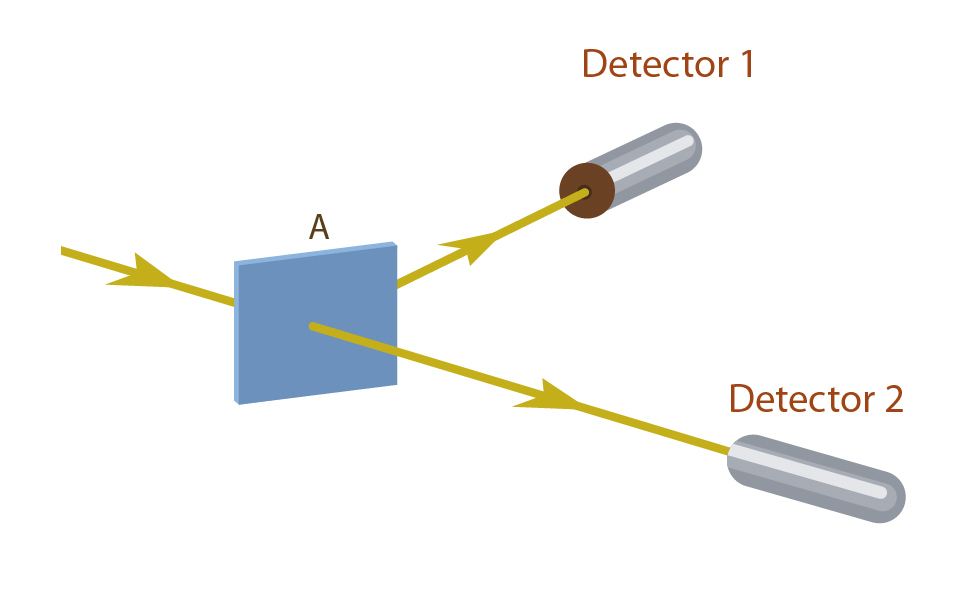
\includegraphics[scale=0.25]{Rationality20From20AI20to20Zombies2020Eliezer20Yudkowsky-img291.jpg}
 \newline
 Figure 230.1
\par}


\bigskip

{
\ \ \ ~}

{
\ \ \ In Figure 230.1, we see, at A, a half-silvered mirror, and two
photon detectors, Detector 1 and Detector 2.}

{
\ \ \ Early scientists, when they ran experiments like this, became
confused about what the results meant. They would send a photon toward
the half-silvered mirror, and half the time they would see Detector 1
click, and the other half of the time they would see Detector 2 click.}

{
\ \ \ The early scientists---you're going to laugh at
this---thought that the silver mirror deflected the photon half the
time, and let it through half the time.}

{
\ \ \ Ha, ha! As if the half-silvered mirror did different things on
different occasions! I want you to let go of this idea, because if you
cling to what early scientists thought, you will become extremely
confused. The half-silvered mirror obeys the same rule every time.}

{
\ \ \ If you were going to write a computer program that \textit{was}
this experiment---not a computer program that \textit{predicted} the
result of the experiment, but a computer program that resembled the
underlying reality---it might look sort of like this:}

{
\ \ \ At the start of the program (the start of the experiment, the
start of time) there's a certain mathematical entity,
called a \textit{configuration}. You can think of this configuration as
corresponding to ``there is one photon heading from
the photon source toward the half-silvered mirror,''
or just ``a photon heading toward
A.''}

{
\ \ \ A configuration can store a single complex
value---``complex'' as in the
complex numbers (a + bi), with i defined as ${\surd}$-1. At the start
of the program, there's already a complex number stored
in the configuration ``a photon heading toward
A.'' The exact value doesn't matter
so long as it's not zero. We'll let the
configuration ``a photon heading toward
A'' have a value of (-1 + 0i).}

{
\ \ \ All this is a fact within the territory, not a description of
anyone's knowledge. A configuration
isn't a proposition or a possible way the world could
be. A configuration is a variable in the program---you can think of it
as a kind of memory location whose index is ``a photon
heading toward A''---and it's out
there in the territory.}

{
\ \ \ As the complex numbers that get assigned to configurations are not
positive real numbers between 0 and 1, there is no danger of confusing
them with probabilities. ``A photon heading toward
A'' has complex value -1, which is hard to see as a
degree of belief. The complex numbers are values within the program,
again out there in the territory. We'll call the
complex numbers \textit{amplitudes.}}

{
\ \ \ There are two other configurations, which we'll
call ``a photon going from A to Detector
1'' and ``a photon going from A to
Detector 2.'' These configurations
don't have a complex value yet; it gets assigned as the
program runs.}

{
\ \ \ We are going to calculate the amplitudes of ``a
photon going from A toward 1'' and
``a photon going from A toward 2''
using the value of ``a photon going toward
A,'' and the rule that describes the half-silvered
mirror at A.}

{
\ \ \ Roughly speaking, the half-silvered mirror rule is
``multiply by 1 when the photon goes straight, and
multiply by i when the photon turns at a right
angle.'' This is the universal rule that relates the
amplitude of the configuration of ``a photon going
in,'' to the amplitude that goes to the
configurations of ``a photon coming out
straight'' or ``a photon being
deflected.''\textsuperscript{1}}

{
\ \ \ So we pipe the amplitude of the configuration ``a
photon going toward A,'' which is (-1 + 0i), into the
half-silvered mirror at A, and this transmits an amplitude of (-1 + 0i)
{\texttimes} i = (0 -i) to ``a photon going from A
toward 1,'' and also transmits an amplitude of (-1 +
0i) {\texttimes} 1 = (-1 + 0i) to ``a photon going
from A toward 2.''}

{
\ \ \ In the Figure 230.1 experiment, these are all the configurations
and all the transmitted amplitude we need to worry about, so
we're done. Or, if you want to think of
``Detector 1 gets a photon'' and
``Detector 2 gets a photon'' as
separate configurations, they'd just inherit their
values from ``A to 1'' and
``A to 2'' respectively. (Actually,
the values inherited should be multiplied by another complex factor,
corresponding to the distance from A to the detector; but we will
ignore that for now, and suppose that all distances traveled in our
experiments happen to correspond to a complex factor of 1.)}

{
\ \ \ So the final program state is:}

{
\ \ \ Configuration ``a photon going toward
A'': (-1 + 0i)}

{
\ \ \ Configuration ``a photon going from A toward
1'': (0 - i)}

{
\ \ \ Configuration ``a photon going from A toward
2'': (-1 + 0i)}

{
\ \ \ \textit{and optionally}}

{
\ \ \ Configuration ``Detector 1 gets a
photon'': (0 - i)}

{
\ \ \ Configuration ``Detector 2 gets a
photon'': (-1 + 0i) .}

{
\ \ \ This same result occurs---the same amplitudes stored in the same
configurations---every time you run the program (every time you do the
experiment).}

{
\ \ \ Now, for \textit{complicated} reasons that we
aren't going to go into here---considerations that
belong on a higher level of organization than fundamental quantum
mechanics, the same way that atoms are more complicated than
quarks---there's no \textit{simple} measuring
instrument that can directly tell us the exact amplitudes of each
configuration. We can't directly see the program
state.}

{
\ \ \ So how do physicists know what the amplitudes are?}

{
\ \ \ We \textit{do} have a magical measuring tool that can tell us the
\textit{squared modulus} of a configuration's
amplitude. If the original complex amplitude is (a + bi), we can get
the positive real number (a\textsuperscript{2} + b\textsuperscript{2}).
Think of the Pythagorean theorem: if you imagine the complex number as
a little arrow stretching out from the origin on a two-dimensional
plane, then the magic tool tells us the squared length of the little
arrow, but it doesn't tell us the direction the arrow
is pointing.}

{
\ \ \ To be more precise, the magic tool actually just tells us the
\textit{ratios} of the squared lengths of the amplitudes in some
configurations. We don't know how long the arrows are
in an absolute sense, just how long they are relative to each other.
But this turns out to be enough information to let us reconstruct the
laws of physics---the rules of the program. And so I can talk about
amplitudes, not just ratios of squared moduli.}

{
\ \ \ When we wave the magic tool over ``Detector 1
gets a photon'' and ``Detector 2
gets a photon,'' we discover that these
configurations have the same squared modulus---the lengths of the
arrows are the same. Thus speaks the magic tool. By doing more
\textit{complicated} experiments (to be seen shortly), we can tell that
the original complex numbers had a ratio of i to 1.}

{
\ \ \ And what is this magical measuring tool?}

{
\ \ \ Well, from the perspective of everyday life---way, way, way above
the quantum level and a lot more complicated---the magical measuring
tool is that we send some photons toward the half-silvered mirror, one
at a time, and count up how many photons arrive at Detector 1 versus
Detector 2 over a few thousand trials. The ratio of these values is the
ratio of the squared moduli of the amplitudes. But the reason for this
is \textit{not} something we are going to consider yet. Walk before you
run. It is not possible to understand what happens \textit{all the way
up} at the level of everyday life, before you understand what goes on
in much simpler cases.}

{
\ \ \ For today's purposes, we have a magical
squared-modulus-ratio reader. And the magic tool tells us that the
little two-dimensional arrow for the configuration
``Detector 1 gets a photon'' has the
same squared length as for ``Detector 2 gets a
photon.'' That's all.}

{
\ \ \ You may wonder, ``Given that the magic tool works
this way, what motivates us to use quantum theory, instead of thinking
that the half-silvered mirror reflects the photon around half the
time?''}

{
\ \ \ Well, that's just begging to be confused---putting
yourself into a historically realistic frame of mind like that and
using everyday intuitions. Did I say anything about a little billiard
ball going one way or the other and possibly bouncing off a mirror?
That's not how reality works. \textit{Reality} is about
complex amplitudes flowing between configurations, and the laws of the
flow are stable.}

{
\ \ \ But if you insist on seeing a more complicated situation that
billiard-ball ways of thinking can't handle,
here's a more complicated experiment.}

{
\ \ \ ~}

{\centering
\ \ \  
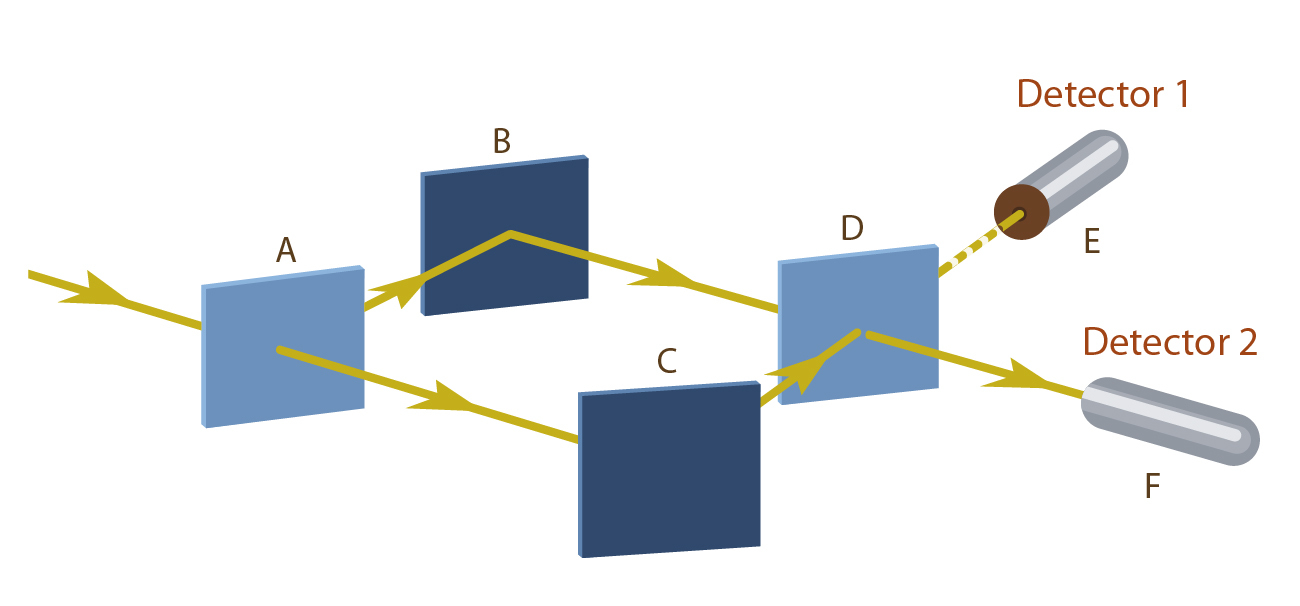
\includegraphics[scale=0.25]{Rationality20From20AI20to20Zombies2020Eliezer20Yudkowsky-img292.jpg}
 \newline
 Figure 230.2
\par}


\bigskip

{
\ \ \ ~}

{
\ \ \ In Figure 230.2, B and C are full mirrors, and A and D are
half-mirrors. The line from D to E is dashed for reasons that will
become apparent, but amplitude is flowing from D to E under exactly the
same laws.}

{
\ \ \ Now let's apply the rules we learned before:}

{
\ \ \ At the beginning of time ``a photon heading
toward A'' has amplitude (-1 + 0i).}

{
\ \ \ We proceed to compute the amplitude for the configurations
``a photon going from A to B'' and
``a photon going from A to C'':}

{\centering
\ \ \ ``a photon going from A to B''
= i {\texttimes} ``a photon heading toward
A'' = (0 $-$ i).
\par}


\bigskip

{
\ \ \ Similarly,}

{\centering
\ \ \ ``a photon going from A to C''
= 1 {\texttimes} ``a photon heading toward
A'' = ($-$1 + 0i).
\par}


\bigskip

{
\ \ \ The full mirrors behave (as one would expect) like half of a
half-silvered mirror---a full mirror just bends things by right angles
and multiplies them by i. (To state this slightly more precisely: For a
full mirror, the amplitude that flows, from the configuration of a
photon heading in, to the configuration of a photon heading out at a
right angle, is multiplied by a factor of i.)}

{
\ \ \ So:}

{\centering
\ \ \ ``a photon going from B to D''
= i {\texttimes} ``a photon going from A to
B'' = (1 + 0i),
\par}


\bigskip

{\centering
\ \ \ ``a photon going from C to D''
= i {\texttimes} ``a photon going from A to
C'' = (0 $-$ i).
\par}


\bigskip

{
\ \ \ ``B to D'' and
``C to D'' are two different
configurations---we don't simply write
``a photon at D''---because the
photons are arriving at two different angles in these two different
configurations. And what D does to a photon depends on the angle at
which the photon arrives.}

{
\ \ \ Again, the rule (speaking loosely) is that when a half-silvered
mirror bends light at a right angle, the amplitude that flows from the
photon-going-in configuration to the photon-going-out configuration, is
the amplitude of the photon-going-in configuration multiplied by i. And
when two configurations are related by a half-silvered mirror letting
light straight through, the amplitude that flows from the
photon-going-in configuration is multiplied by 1.}

{
\ \ \ So:}

{
\ \ \ From the configuration ``a photon going from B to
D,'' with original amplitude (1 + 0i): Amplitude of
(1 + 0i) {\texttimes} i = (0 + i) flows to ``a photon
going from D to E.'' Amplitude of (1 + 0i)
{\texttimes} 1 = (1 + 0i) flows to ``a photon going
from D to F.'' }

{
\ \ \ From the configuration ``a photon going from C to
D,'' with original amplitude (0 - i): Amplitude of (0
-i) {\texttimes} i = (1 + 0i) flows to ``a photon
going from D to F.'' Amplitude of (0 - i)
{\texttimes} 1 = (0 - i) flows to ``a photon going
from D to E.'' }

{
\ \ \ Therefore:}

{
\ \ \ The \textit{total} amplitude flowing to configuration
``a photon going from D to E'' is (0
+ i) + (0 - i) = (0 + 0i) = 0.}

{
\ \ \ The total amplitude flowing to configuration ``a
photon going from D to F'' is (1 + 0i) + (1 + 0i) =
(2 + 0i).}

{
\ \ \ (You may want to try working this out yourself on pen and paper if
you lost track at any point.)}

{
\ \ \ But the upshot, from that super-high-level
``experimental'' perspective that we
think of as normal life, is that we see \textit{no} photons detected at
E. Every photon seems to end up at F. The ratio of squared moduli
between ``D to E'' and
``D to F'' is 0 to 4.
That's why the line from D to E is dashed, in this
figure.}

{
\ \ \ This is not something it is possible to explain by thinking of
half-silvered mirrors deflecting little incoming billiard balls half
the time. You've \textit{got} to think in terms of
amplitude flows.}

{
\ \ \ If half-silvered mirrors deflected a little billiard ball half the
time, in this setup, the little ball would end up at Detector 1 around
half the time and Detector 2 around half the time. Which it
doesn't. So don't think that.}

{
\ \ \ You may say, ``But wait a minute! I can think of
another hypothesis that accounts for this result. What if, when a
half-silvered mirror reflects a photon, it does something to the photon
that ensures it doesn't get reflected next time? And
when it lets a photon go through straight, it does something to the
photon so it gets reflected next time.''}

{
\ \ \ Now really, there's no need to go making the rules
so complicated. Occam's Razor, remember. Just stick
with simple, normal amplitude flows between configurations.}

{
\ \ \ But if you want \textit{another} experiment that disproves your
\textit{new} alternative hypothesis, it's Figure
230.3.}

{
\ \ \ ~}

{\centering
\ \ \  
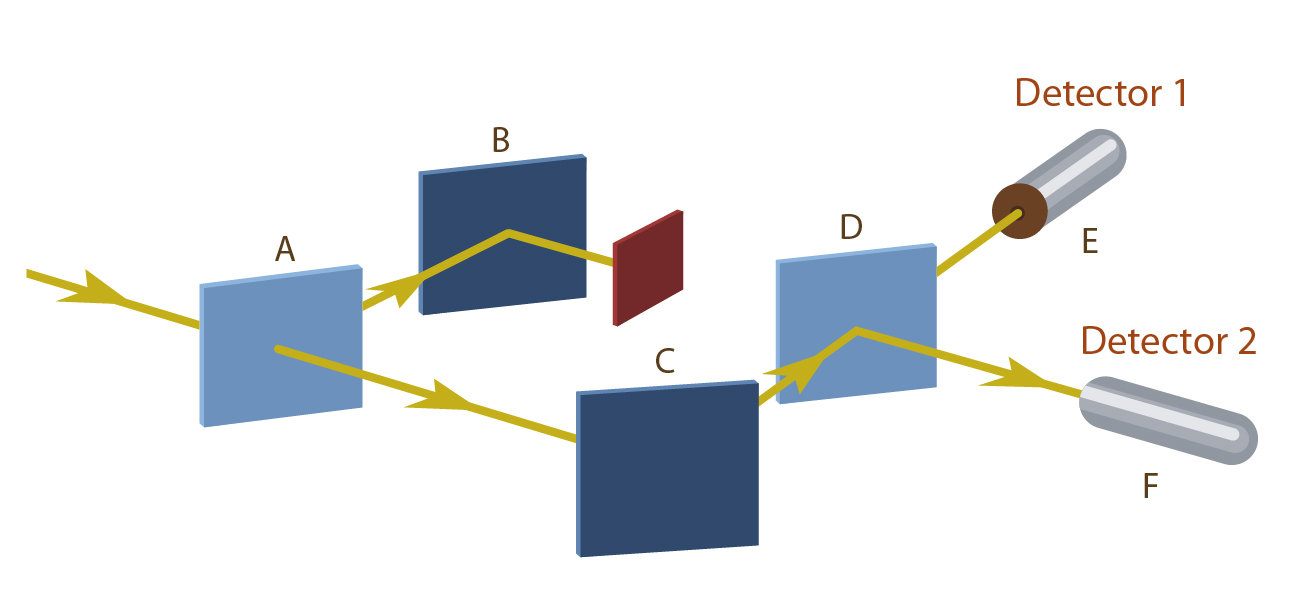
\includegraphics[scale=0.25]{Rationality20From20AI20to20Zombies2020Eliezer20Yudkowsky-img293.jpg}
 \newline
 Figure 230.3
\par}


\bigskip

{
\ \ \ ~}

{
\ \ \ Here, we've left the whole experimental setup the
same, and just put a little blocking object between B and D. This
ensures that the amplitude of ``a photon going from B
to D'' is 0.}

{
\ \ \ Once you eliminate the amplitude contributions from that
configuration, you end up with totals of (1 + 0i) in
``a photon going from D to F,'' and
(0 -i) in ``a photon going from D to
E.''}

{
\ \ \ The squared moduli of (1 + 0i) and (0 - i) are both 1, so the
magic measuring tool should tell us that the ratio of squared moduli is
1. Way back up at the level where physicists exist, we should find that
Detector 1 goes off half the time, and Detector 2 half the time.}

{
\ \ \ The same thing happens if we put the block between C and D. The
amplitudes are different, but the ratio of the squared moduli is still
1, so Detector 1 goes off half the time and Detector 2 goes off half
the time.}

{
\ \ \ This cannot \textit{possibly} happen with a little billiard ball
that either does or doesn't get reflected by the
half-silvered mirrors.}

{
\ \ \ Because complex numbers can have opposite directions, like 1 and
-1, or i and -i, amplitude flows can cancel each other out. Amplitude
flowing from configuration X into configuration Y can be canceled out
by an equal and opposite amplitude flowing from configuration Z into
configuration Y. In fact, that's exactly what happens
in this experiment.}

{
\ \ \ In probability theory, when something can either happen one way or
another, X or {\textlnot}X, then P(Z) = P(Z{\textbar}X)P(X) +
P(Z{\textbar}{\textlnot}X)P({\textlnot}X). And all probabilities are
positive. So if you establish that the probability of Z happening given
X is 1$/$2, and the probability of X happening is 1$/$3, then the total
probability of Z happening is \textit{at least} 1$/$6 no matter
\textit{what} goes on in the case of {\textlnot}X.
There's no such thing as negative probability,
less-than-impossible credence, or (0 + i) credibility, so
\textit{degrees of belief} can't cancel each other out
like amplitudes do.}

{
\ \ \ Not to mention that probability is in the mind to begin with; and
we are talking \textit{about} the territory, the
program-that-is-reality, not talking \textit{about} human cognition or
states of partial knowledge.}

{
\ \ \ By the same token, configurations are not \textit{propositions},
not \textit{statements}, not \textit{ways the world could conceivably
be}. Configurations are not semantic constructs. Adjectives like
\textit{probable} do not apply to them; they are not beliefs or
sentences or possible worlds. They are not \textit{true} or
\textit{false} but simply \textit{real}.}

{
\ \ \ In the experiment of Figure 230.2, do not be tempted to think
anything like: ``The photon goes to either B or C, but
it \textit{could} have gone the other way, and this possibility
interferes with its ability to go to E .~.~.''}

{
\ \ \ It makes no sense to think of something that
``could have happened but
didn't'' exerting an effect on the
world. We can \textit{imagine} things that could have happened but
didn't---like thinking, ``Gosh, that
car almost hit me''---and our imagination can have an
effect on our future behavior. But the event of imagination is a real
event, that actually happens, and \textit{that} is what has the effect.
It's your imagination of the unreal event---your very
real imagination, implemented within a quite physical brain---that
affects your behavior.}

{
\ \ \ To think that the \textit{actual event} of a car hitting
you---this event which could have happened to you, but in fact
didn't---is directly exerting a \textit{causal} effect
on your behavior, is mixing up the map with the territory.}

{
\ \ \ What affects the world is real. (If things can affect the world
without being ``real,''
it's hard to see what the word
``real'' means.) Configurations and
amplitude flows are causes, and they have visible effects; they are
real. Configurations are not possible worlds and amplitudes are not
degrees of belief, any more than your chair is a possible world or the
sky is a degree of belief.}

{
\ \ \ So what \textit{is} a configuration, then?}

{
\ \ \ Well, you'll be getting a clearer idea of that in
later essays.}

{
\ \ \ But to give you a quick idea of how the real picture differs from
the simplified version we saw in this essay .~.~.}

{
\ \ \ Our experimental setup only dealt with one moving particle, a
single photon. Real configurations are about multiple particles. The
next essay will deal with the case of more than one particle, and that
should give you a much clearer idea of what a configuration is.}

{
\ \ \ Each configuration we talked about \textit{should} have described
a joint position of all the particles in the mirrors and detectors, not
just the position of one photon bopping around.}

{
\ \ \ In fact, the \textit{really real} configurations are over joint
positions of all the particles in the universe, including the particles
making up the experimenters. You can see why I'm saving
the notion of \textit{experimental results} for later essays.}

{
\ \ \ In the real world, amplitude is a continuous distribution over a
continuous \textit{space} of configurations. This
essay's
``configurations'' were blocky and
digital, and so were our ``amplitude
flows.'' It was as if we were talking about a photon
teleporting from one place to another.}

{
\ \ \ If none of that made sense, don't worry. It will
be cleared up in later essays. Just wanted to give you some idea of
where this was heading.}

{\centering
\ \ \ \ ~
\par}

{\centering
\ \ \ *
\par}


\bigskip

{
\ \ \ 1. \textbf{Editor's Note:} Strictly speaking, a
standard half-silvered mirror would yield a rule
``multiply by -1 when the photon turns at a right
angle,'' not ``multiply by
i.'' The basic scenario described by the author is
not physically impossible, and its use does not affect the substantive
argument. However, physics students may come away confused if they
compare the discussion here to textbook discussions of Mach--Zehnder
interferometers. We've left this idiosyncrasy in the
text because it eliminates any need to specify which side of the mirror
is half-silvered, simplifying the experiment.}

\mysection{Joint Configurations}

{
\ \ \ The key to understanding configurations, and hence the key to
understanding quantum mechanics, is realizing on a truly gut level that
configurations are about more than one particle.}

{
\ \ \ ~}

{\centering
\ \ \  
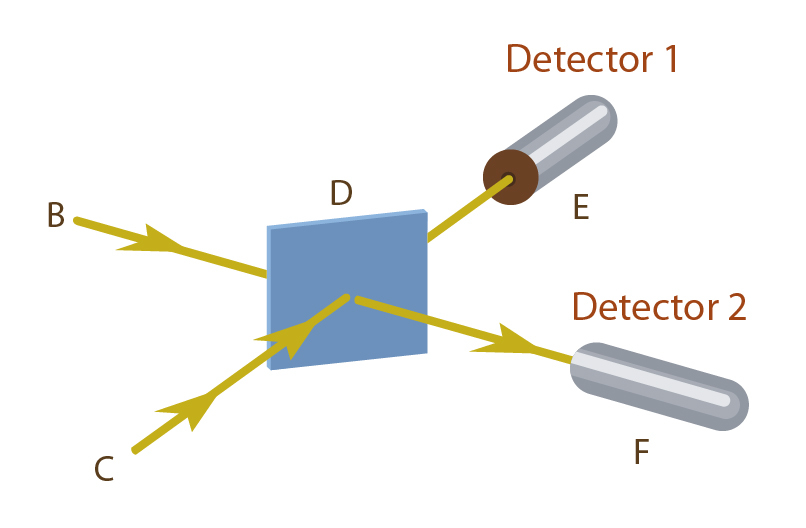
\includegraphics[scale=0.25]{Rationality20From20AI20to20Zombies2020Eliezer20Yudkowsky-img295.jpg}
 \newline
 Figure 231.1
\par}


\bigskip

{
\ \ \ ~}

{
\ \ \ Continuing from the previous essay, Figure 231.1 shows an altered
version of the experiment where we send in \textit{two} photons toward
D at the same time, from the sources B and C.}

{
\ \ \ The starting configuration then is:}

{
\ \ \ ``a photon going from B to D,\newline
 and a photon going from C to D.''}

{
\ \ \ Again, let's say the starting configuration has
amplitude (-1 + 0i).}

{
\ \ \ And remember, the rule of the half-silvered mirror (at D) is that
a right-angle deflection multiplies by i, and a straight line
multiplies by 1.}

{
\ \ \ So the amplitude flows from the starting configuration, separately
considering the four cases of deflection/non-deflection of each photon,
are:}

{
\ \ \ The ``B to D'' photon is
deflected and the ``C to D'' photon
is deflected. This amplitude flows to the configuration
``a photon going from D to E, and a photon going from
D to F.'' The amplitude flowing is (-1 + 0i)
{\texttimes} i {\texttimes} i = (1 + 0i).}

{
\ \ \ The ``B to D'' photon is
deflected and the ``C to D'' photon
goes straight. This amplitude flows to the configuration
``two photons going from D to E.''
The amplitude flowing is (-1 + 0i) {\texttimes} i {\texttimes} 1 = (0 -
i).}

{
\ \ \ The ``B to D'' photon goes
straight and the ``C to D'' photon
is deflected. This amplitude flows to the configuration
``two photons going from D to F.''
The amplitude flowing is (-1 + 0i) {\texttimes} 1 {\texttimes} i = (0 -
i).}

{
\ \ \ The ``B to D'' photon goes
straight and the ``C to D'' photon
goes straight. This amplitude flows to the configuration
``a photon going from D to F, and a photon going from
D to E.'' The amplitude flowing is (-1 + 0i)
{\texttimes} 1 {\texttimes} 1 = (-1 + 0i).}

{
\ \ \ Now---and this is a \textit{very important and fundamental idea in
quantum mechanics}{}---the amplitudes in cases 1 and 4 are flowing to
the \textit{same} configuration. Whether the B photon and C photon both
go straight, or both are deflected, the resulting configuration is
\textit{one photon going toward E and another photon going toward F}.}

{
\ \ \ So we add up the two incoming amplitude flows from case 1 and case
4, and get a total amplitude of (1 + 0i) + (-1 + 0i) = 0.}

{
\ \ \ When we wave our magic squared-modulus-ratio reader over the three
final configurations, we'll find that
``two photons at Detector 1'' and
``two photons at Detector 2'' have
the same squared modulus, but ``a photon at Detector 1
and a photon at Detector 2'' has squared modulus
zero.}

{
\ \ \ Way up at the level of experiment, we never find Detector 1 and
Detector 2 both going off. We'll find Detector 1 going
off twice, or Detector 2 going off twice, with equal frequency.
(Assuming I've gotten the math and physics right. I
didn't actually perform the experiment.)}

{
\ \ \ The configuration's identity is \textit{not},
``the B photon going toward E and the C photon going
toward F.'' Then the resultant configurations in case
1 and case 4 would not be equal. Case 1 would be, ``B
photon to E, C photon to F'' and case 4 would be
``B photon to F, C photon to E.''
These would be two distinguishable configurations, \textit{if}
configurations had photon-tracking structure.}

{
\ \ \ So we would not add up the two amplitudes and cancel them out. We
would keep the amplitudes in two separate configurations. The total
amplitudes would have non-zero squared moduli. And when we ran the
experiment, we would find (around half the time) that Detector 1 and
Detector 2 each registered one photon. Which doesn't
happen, if my calculations are correct.}

{
\ \ \ Configurations don't keep track of where particles
come from. A configuration's identity is just,
``a photon here, a photon there; an electron here, an
electron there.'' No matter how you get into that
situation, so long as there are the same species of particles in the
same places, it counts as the same configuration.}

{
\ \ \ I say again that the question ``What kind of
information does the configuration's structure
incorporate?'' has \textit{experimental
consequences.} You can deduce, from experiment, the way that reality
itself must be treating configurations.}

{
\ \ \ In a classical universe, there would be no experimental
consequences. If the photon were like a little billiard ball that
either went one way or the other, and the configurations were our
beliefs about possible states the system could be in, and instead of
amplitudes we had probabilities, it would not make a difference whether
we tracked the origin of photons or threw the information away.}

{
\ \ \ In a classical universe, I could assign a 25\% probability to both
photons going to E, a 25\% probability of both photons going to F, a
25\% probability of the B photon going to E and the C photon going to
F, and 25\% probability of the B photon going to F and the C photon
going to E. Or, since I \textit{personally} don't care
which of the two latter cases occurred, I could decide to collapse the
two possibilities into one possibility and add up their probabilities,
and just say, ``a 50\% probability that each detector
gets one photon.''}

{
\ \ \ With probabilities, we can aggregate events as we like---draw our
boundaries around sets of possible worlds as we please---and the
numbers will still work out the same. The probability of two mutually
exclusive events always equals the probability of the first event plus
the probability of the second event.}

{
\ \ \ But you can't arbitrarily collapse configurations
together, or split them apart, in your model, and get the same
experimental predictions. Our magical tool tells us the ratios of
squared moduli. When you add two complex numbers, the squared modulus
of the sum is not the sum of the squared moduli of the parts:}

{\centering
\ \ \ Squared\_Modulus(C1 + C2) ${\neq}$ Squared\_Modulus(C1) +
Squared\_Modulus(C2).
\par}


\bigskip

{
\ \ \ E.g.:}

{\centering
\ \ \ S\_M((2 + i) + (1 $-$ i)) = S\_M(3 + 0i)\newline
 = 3\textsuperscript{2} + 0\textsuperscript{2}\newline
 = 9,
\par}


\bigskip

{\centering
\ \ \ S\_M(2 + i) + S\_M(1 $-$ i) = (2\textsuperscript{2} +
1\textsuperscript{2})+ ( 1\textsuperscript{2} +
(-1)\textsuperscript{2})\newline
 = (4 + 1) + (1 + 1)\newline
 = 7.
\par}


\bigskip

{
\ \ \ Or in the current experiment of discourse, we had flows of (1 +
0i) and (-1 + 0i) cancel out, adding up to 0, whose squared modulus is
0, where the squared modulus of the parts would have been 1 and 1.}

{
\ \ \ If in place of Squared\_Modulus, our magical tool was some linear
function---any function where F(X + Y) = F(X) + F(Y)---then all the
quantumness would instantly vanish and be replaced by a classical
physics. (A \textit{different} classical physics, not the same illusion
of classicality we hallucinate from inside the higher levels of
organization in our own quantum world.)}

{
\ \ \ If amplitudes were just probabilities, they
couldn't cancel out when flows collided. If
configurations were just states of knowledge, you could reorganize them
however you liked.}

{
\ \ \ But the configurations are nailed in place, indivisible and
unmergeable without changing the laws of physics.}

{
\ \ \ And part of what is nailed is the way that configurations treat
multiple particles. A configuration says, ``a photon
here, a photon there,'' not
``\textit{this} photon here, \textit{that} photon
there.'' ``\textit{This} photon
here, \textit{that} photon there'' does not have a
different identity from ``\textit{that} photon here,
\textit{this} photon there.''}

{
\ \ \ The result, visible in today's experiment, is that
you can't factorize the physics of our universe to be
about particles with individual identities.}

{
\ \ \ Part of the reason why humans have trouble coming to grips with
\textit{perfectly normal} quantum physics, is that humans bizarrely
keep trying to factor reality into a sum of individually real billiard
balls.}

{
\ \ \ Ha ha! Silly humans.}

{\centering
\ \ \ \ ~
\par}

{\centering
\ \ \ *
\par}

\mysection{Distinct Configurations}

{
\ \ \ The experiment in the previous essay carried two key lessons: }

{
\ \ \ First, we saw that because amplitude flows can cancel out, and
because our magic measure of squared modulus is not linear, the
identity of configurations is nailed down---you can't
reorganize configurations the way you can regroup possible worlds.
Which configurations are the same, and which are distinct, has
experimental consequences; it is an observable fact.}

{
\ \ \ Second, we saw that configurations are about multiple particles.
If there are two photons entering the apparatus, that
doesn't mean there are two initial configurations.
Instead the initial configuration's identity is
``two photons coming in.'' (Ideally,
each configuration we talk about would include every particle in the
experiment---including the particles making up the mirrors and
detectors. And in the real universe, every configuration is about
\textit{all} the particles .~.~. \textit{everywhere}.)}

{
\ \ \ What makes for distinct configurations is not distinct particles.
Each configuration is about every particle. What makes configurations
distinct is particles occupying different positions---at least one
particle in a different state.}

{
\ \ \ To take one important demonstration .~.~.}

{
\ \ \ ~}

{\centering
\ \ \  
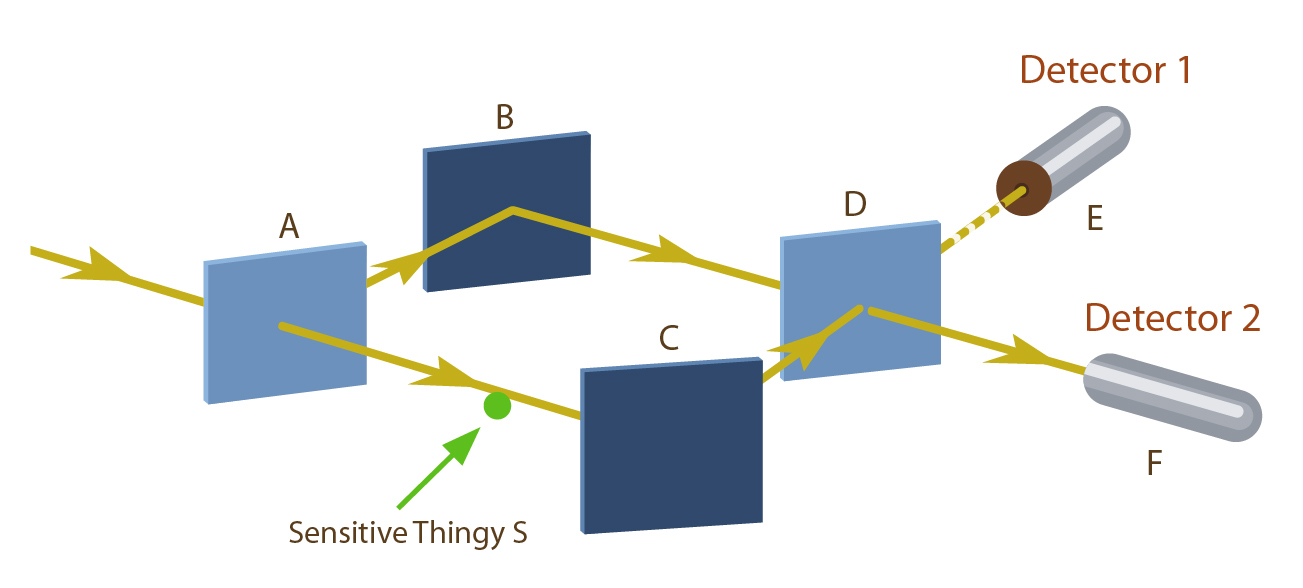
\includegraphics[scale=0.25]{Rationality20From20AI20to20Zombies2020Eliezer20Yudkowsky-img297.jpg}
 \newline
 Figure 232.1
\par}


\bigskip

{
\ \ \ ~}

{
\ \ \ Figure 232.1 is the same experiment as Figure 230.2, with one
important change: Between A and C has been placed a sensitive thingy,
S. The key attribute of S is that if a photon goes past S, then S ends
up in a slightly different state.}

{
\ \ \ Let's say that the two possible states of S are
\textit{Yes} and \textit{No}. The sensitive thingy S starts out in
state \textit{No}, and ends up in state \textit{Yes} if a photon goes
past.}

{
\ \ \ Then the initial configuration is:}

{
\ \ \ ``photon heading toward A; and S in state
\textit{No},'' (-1 + 0i) .}

{
\ \ \ Next, the action of the half-silvered mirror at A. In the previous
version of this experiment, without the sensitive thingy, the two
resultant configurations were ``A to
B'' with amplitude -i and ``A to
C'' with amplitude -1. Now, though, a new element has
been introduced into the system, and all configurations are about all
particles, and so every configuration mentions the new element. So the
amplitude flows from the initial configuration are to:}

{
\ \ \ ``photon from A to B; and S in state
\textit{No},'' (0 - i)}

{
\ \ \ ``photon from A to C; and S in state
\textit{Yes},'' (-1 + 0i) .}

{
\ \ \ Next, the action of the full mirrors at B and C:}

{
\ \ \ ``photon from B to D; and S in state
\textit{No},'' (1 + 0i)}

{
\ \ \ ``photon from C to D; and S in state
\textit{Yes},'' (0 - i) .}

{
\ \ \ And then the action of the half-mirror at D, on the amplitude
flowing from both of the above configurations:}

{
\ \ \ ``photon from D to E; and S in state
\textit{No},'' (0 + i)}

{
\ \ \ ``photon from D to F; and S in state
\textit{No},'' (1 + 0i)}

{
\ \ \ ``photon from D to E; and S in state
\textit{Yes},'' (0 - i)}

{
\ \ \ ``photon from D to F; and S in state
\textit{Yes},'' (1 + 0i) .}

{
\ \ \ When we did this experiment without the sensitive thingy, the
amplitude flows (1) and (3) of (0 + i) and (0 - i) to the
``D to E'' configuration canceled
each other out. We were left with no amplitude for a photon going to
Detector 1 (way up at the experimental level, we never observe a photon
striking Detector 1).}

{
\ \ \ But in this case, the two amplitude flows (1) and (3) are now to
distinct configurations; at least one entity, S, is in a different
state between (1) and (3). The amplitudes don't cancel
out.}

{
\ \ \ When we wave our magical squared-modulus-ratio detector over the
four final configurations, we find that the squared moduli of all are
equal: 25\% probability each. Way up at the level of the real world, we
find that the photon has an equal chance of striking Detector 1 and
Detector 2.}

{
\ \ \ All the above is true, even if we, the researchers,
don't care about the state of S. Unlike possible
worlds, configurations cannot be regrouped on a whim. The laws of
\textit{physics} say the two configurations are distinct;
it's not a question of how \textit{we} can most
conveniently parse up the world.}

{
\ \ \ All the above is true, even if we don't bother to
look at the state of S. The configurations (1) and (3) are distinct in
physics, even if we don't know the distinction.}

{
\ \ \ All the above is true, even if we don't know S
exists. The configurations (1) and (3) are distinct whether or not
\textit{we} have distinct \textit{mental representations} for the two
possibilities.}

{
\ \ \ All the above is true, even if we're in space, and
S transmits a new photon off toward the interstellar void in two
distinct directions, depending on whether the photon of interest passed
it or not. So that we couldn't \textit{ever} find out
whether S had been in \textit{Yes} or \textit{No}. The state of S would
be embodied in the photon transmitted off to nowhere. The lost photon
can be an implied invisible, and the state of S pragmatically
undetectable; but the configurations are still distinct.}

{
\ \ \ (The main reason it \textit{wouldn't} work, is if
S were nudged, but S had an original spread in configuration space that
was larger than the nudge. Then you couldn't rely on
the nudge to separate the amplitude distribution over configuration
space into distinct lumps. In reality, all this takes place within a
differentiable amplitude distribution over a continuous configuration
space.)}

{
\ \ \ Configurations are not belief states. Their distinctness is an
objective fact with experimental consequences. The configurations are
distinct even if no one knows the state of S; distinct even if no
intelligent entity can ever find out. The configurations are distinct
so long as at least \textit{one particle} in the universe
\textit{anywhere} is in a different position. This is experimentally
demonstrable.}

{
\ \ \ Why am I emphasizing this? Because back in the dark ages when no
one understood quantum physics .~.~.}

{
\ \ \ ~}

{\centering
\ \ \  
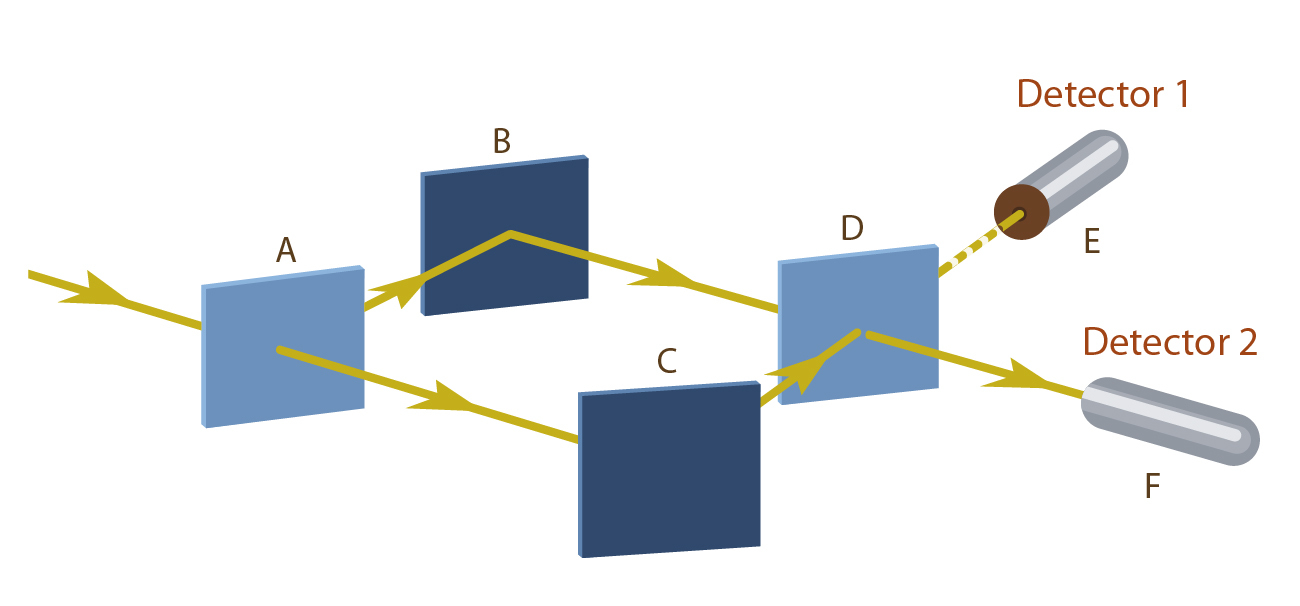
\includegraphics[scale=0.25]{Rationality20From20AI20to20Zombies2020Eliezer20Yudkowsky-img292.jpg}
 \newline
 Figure 232.2
\par}


\bigskip

{
\ \ \ ~}

{
\ \ \ Okay, so imagine that you've got no clue
what's really going on, and you try the experiment in
Figure 232.2, and no photons show up at Detector 1. Cool.}

{
\ \ \ You also discover that when you put a block between B and D,
\textit{or} a block between A and C, photons show up at Detector 1 and
Detector 2 in equal proportions. But only one at a time---Detector 1 or
Detector 2 goes off, not both simultaneously.}

{
\ \ \ So, yes, it \textit{does} seem to you like you're
dealing with a particle---the photon is only in one place at one time,
every time \textit{you} see it.}

{
\ \ \ And yet there's some kind of .~.~.
\textit{mysterious phenomenon .~.~.} that prevents the photon from
showing up in Detector 1. And this mysterious phenomenon depends on the
photon being \textit{able} to go both ways. Even though the photon only
shows up in one detector or the other, which shows, \textit{you would
think,} that the photon is only in one place at a time.}

{
\ \ \ ~}

{\centering
\ \ \  
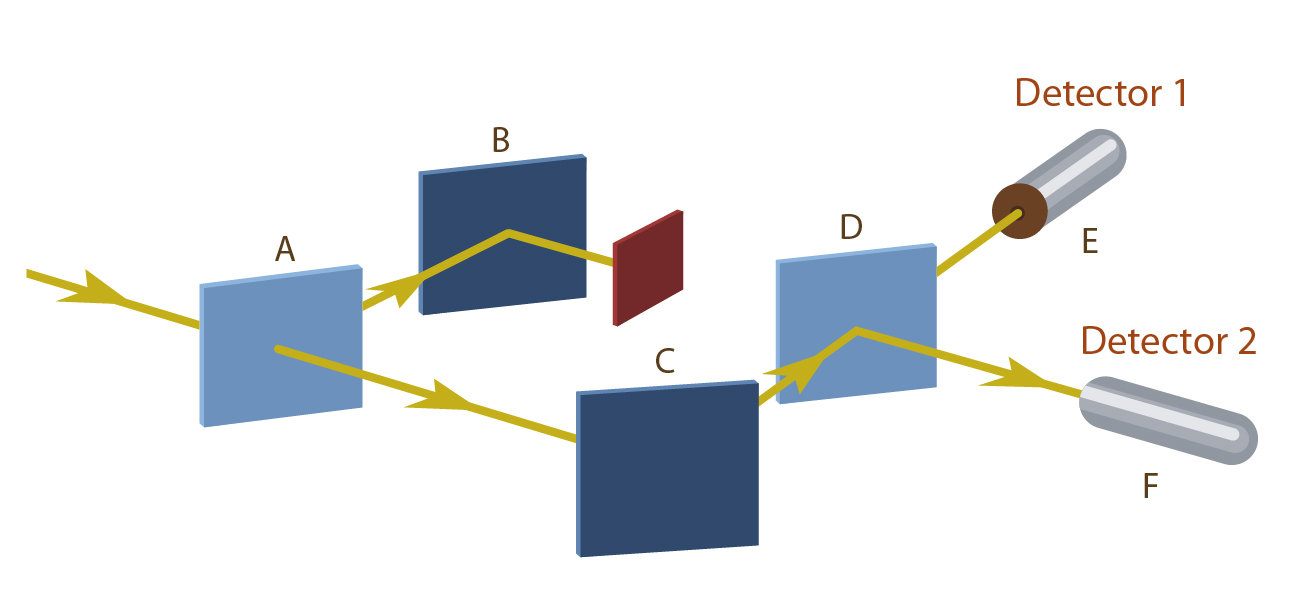
\includegraphics[scale=0.25]{Rationality20From20AI20to20Zombies2020Eliezer20Yudkowsky-img293.jpg}
 \newline
 Figure 232.3
\par}


\bigskip

{
\ \ \ ~}

{
\ \ \ Which makes the whole pattern of the experiments seem pretty
bizarre! After all, the photon either goes from A to C, or from A to B;
one or the other. (Or so you would think, if you were instinctively
trying to break reality down into individually real particles.) But
when you block off one course or the other, as in Figure 232.3, you
start getting different experimental results!}

{
\ \ \ It's like the photon wants to be \textit{allowed}
to go both ways, even though (you would think) it only goes one way or
the other. And it can \textit{tell} if you try to block it off, without
actually going \textit{there}{}---if it'd gone there,
it would have run into the block, and not hit any detector at all.}

{
\ \ \ It's as if mere \textit{possibilities} could have
causal effects, in defiance of what the word
``real'' is usually thought to
\textit{mean} .~.~.}

{
\ \ \ But it's a bit early to jump to conclusions like
\textit{that}, when you don't have a complete picture
of what goes on inside the experiment.}

{
\ \ \ ~}

{\centering
\ \ \  
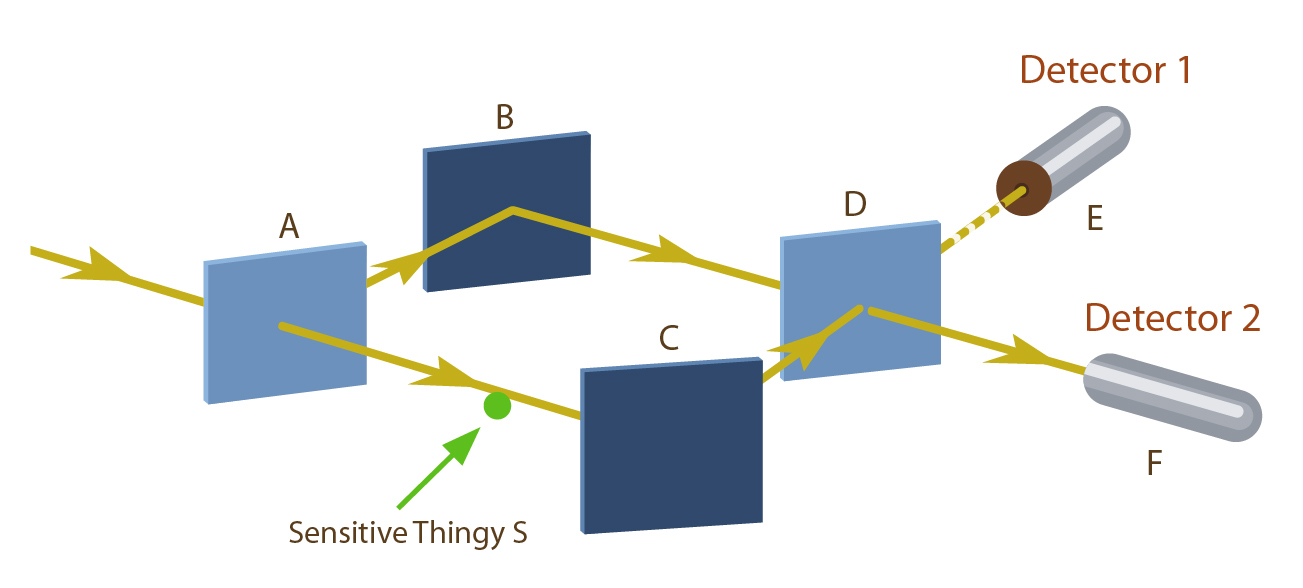
\includegraphics[scale=0.25]{Rationality20From20AI20to20Zombies2020Eliezer20Yudkowsky-img297.jpg}
 \newline
 Figure 232.4
\par}


\bigskip

{
\ \ \ ~}

{
\ \ \ So it occurs to you to put a sensor between A and C, like in
Figure 232.4, so you can tell which way the photon \textit{really} goes
on each occasion.}

{
\ \ \ And the mysterious phenomenon goes away.}

{
\ \ \ I mean, now how crazy is that? What kind of paranoia does that
inspire in some poor scientist?}

{
\ \ \ Okay, so in the twenty-first century we realize in order to
``know'' a photon's
history, the particles making up your brain have to be correlated with
the photon's history. If having a tiny little sensitive
thingy S that correlates to the photon's history is
enough to distinguish the final configurations and prevent the
amplitude flows from canceling, then an entire sensor with a digital
display, never mind a human brain, will put \textit{septillions} of
particles in different positions and prevent the amplitude flows from
canceling.}

{
\ \ \ But if you hadn't worked that out yet .~.~.}

{
\ \ \ Then you would ponder the sensor having banished the Mysterious
Phenomenon, and think:}

{
\ \ \ The photon doesn't just want to be
\textit{physically} free to go either way. It's not a
little wave going along an unblocked pathway, because then just having
a physically unblocked pathway would be enough.}

{
\ \ \ No .~.~. I'm not allowed to \textit{know} which
way the photon went.}

{
\ \ \ The mysterious phenomenon .~.~. \textit{doesn't
want me looking at it too closely} .~.~. while it's
doing its mysterious thing.}

{
\ \ \ It's not \textit{physical possibilities} that have
an effect on reality .~.~. only \textit{epistemic possibilities.} If I
\textit{know} which way the photon went, it's no longer
\textit{plausible} that it went the other way .~.~. which cuts off the
mysterious phenomenon as effectively as putting a block between B and
D.}

{
\ \ \ I have to \textit{not observe} which way the photon went, in order
for it to always end up at Detector 2. It has to be \textit{reasonable}
that the photon could have gone to either B or C. What I can
\textit{know} is the determining factor, regardless of which physical
paths I leave open or closed.}

{
\ \ \ STOP THE PRESSES! MIND IS FUNDAMENTAL AFTER ALL! CONSCIOUS
AWARENESS DETERMINES OUR EXPERIMENTAL RESULTS!}

{
\ \ \ You can \textit{still read} this kind of stuff. In \textit{physics
textbooks.} Even now, when a majority of theoretical physicists know
better. Stop the presses. Please, stop the presses.}

{
\ \ \ Hindsight is 20/20; and so it's easy to say that,
in hindsight, there were certain clues that this interpretation was not
correct.}

{
\ \ \ Like, if you put the sensor between A and C \textit{but
don't read it}, the mysterious phenomenon
\textit{still} goes away, and the photon still sometimes ends up at
Detector 1. (Oh, but you \textit{could} have read it, and possibilities
are real now .~.~.)}

{
\ \ \ But it doesn't even have to be a \textit{sensor},
a scientific instrument that you built. A single particle that gets
nudged far enough will dispel the interference. A photon radiating off
to where you'll never see it again can do the trick.
Not much human involvement there. Not a whole lot of conscious
awareness.}

{
\ \ \ Maybe before you pull the dualist fire alarm on human brains being
physically special, you should provide experimental proof that a rock
can't play the same role in dispelling the Mysterious
Phenomenon as a human researcher?}

{
\ \ \ But that's hindsight, and it's
easy to call the shots in hindsight. Do you \textit{really} think you
could've done better than John von Neumann, if
you'd been alive at the time? The point of this kind of
retrospective analysis is to ask what kind of fully general clues you
could have followed, and whether there are any similar clues
you're ignoring now on current mysteries.}

{
\ \ \ Though it \textit{is} a little embarrassing that even
\textit{after} the theory of amplitudes and configurations had been
worked out---with the theory now giving the definite prediction that
any nudged particle would do the trick---early scientists
\textit{still} didn't get it.}

{
\ \ \ But you see .~.~. it had been established as Common Wisdom that
configurations were possibilities, it was epistemic possibility that
mattered, amplitudes were a very strange sort of partial information,
and conscious observation made quantumness go away. And that it was
best to avoid thinking too hard about the whole business, so long as
your experimental predictions came out right.}

{\centering
\ \ \ \ ~
\par}

{\centering
\ \ \ *
\par}

\mysection{Collapse Postulates}

{
\ \ \ Macroscopic decoherence{}---also known as
``many-worlds''---is the idea that
the known quantum laws that govern microscopic events simply govern at
all levels without alteration. Back when people didn't
know about decoherence---before it occurred to anyone that the laws
deduced with such precision for microscopic physics might apply
universally---what did people \textit{think} was going on? }

{
\ \ \ The initial reasoning seems to have gone something like:}

{
\ \ \ When my calculations showed an amplitude of (-1$/$3)i for this
photon to get absorbed, my experimental statistics showed that the
photon was absorbed around 107 times out of 1,000, which is a good fit
to 1$/$9, the square of the modulus.}

{
\ \ \ to}

{
\ \ \ The amplitude \textit{is} the probability (by way of the squared
modulus).}

{
\ \ \ to}

{
\ \ \ Once you measure something and \textit{know it
didn't happen}, its \textit{probability} goes to zero.}

{
\ \ \ Read literally, this implies that knowledge itself---or even
conscious awareness---causes the collapse. Which was in fact the form
of the theory put forth by Werner Heisenberg!}

{
\ \ \ But people became increasingly nervous about the notion of
importing dualistic language into fundamental physics---as well they
should have been! And so the original reasoning was replaced by the
notion of an objective ``collapse''
that destroyed all parts of the wavefunction except one, and was
triggered sometime before superposition grew to human-sized levels.}

{
\ \ \ Now, once you're supposing that parts of the
wavefunction can just vanish, you might think to ask:}

{
\ \ \ Is there only \textit{one} survivor? Maybe there are many
surviving worlds, but they survive with a frequency determined by their
integrated squared modulus, and so the typical surviving world has
experimental statistics that match the Born rule.}

{
\ \ \ Yet collapse theories considered in modern academia only postulate
\textit{one} surviving world. Why?}

{
\ \ \ Collapse theories were devised in a time when it \textit{simply
didn't occur} to any physicists that more than one
world \textit{could} exist! People took for granted that measurements
had single outcomes---it was an assumption so deep it was invisible,
because it was what they \textit{saw happening.} Collapse theories were
devised to explain \textit{why measurements had single outcomes},
rather than (in full generality) \textit{why experimental statistics
matched the Born rule.}}

{
\ \ \ For similar reasons, the ``collapse
postulates'' considered academically suppose that
collapse occurs \textit{before} any human beings get superposed. But
experiments are steadily ruling out the possibility of
``collapse'' in increasingly large
entangled systems. Apparently an experiment is underway to demonstrate
quantum superposition at 50-micrometer scales, which is bigger than
most neurons and getting up toward the diameter of some human hairs!}

{
\ \ \ So why doesn't someone try jumping ahead of the
game, and ask:}

{
\ \ \ Say, we keep having to postulate the collapse occurs steadily
later and later. What if collapse occurs only once superposition
reaches planetary scales and substantial divergence occurs---say,
Earth's wavefunction collapses around once a minute?
Then, while the surviving Earths at any given time would
\textit{remember} a long history of quantum experiments that matched
the Born statistics, a supermajority of those Earths would begin
obtaining non-Born results from quantum experiments and then abruptly
cease to exist a minute later.}

{
\ \ \ Why don't collapse theories like \textit{that} one
have a huge academic following, among the many people who apparently
think it's okay for parts of the wavefunction to just
vanish? Especially given that experiments are proving superposition in
steadily larger systems?}

{
\ \ \ A cynic might suggest that the reason for
collapse's continued support isn't the
\textit{physical plausibility} of having large parts of the
wavefunction suddenly vanish, or the hope of somehow explaining the
Born statistics. The point is to keep the intuitive appeal of
``I don't remember the measurement
having more than one result, therefore only one thing happened; I
don't remember splitting, so there must be only one of
me.'' You don't remember dying, so
superposed humans must never collapse. A theory that dared to stomp on
intuition would be missing the whole point. You might as well just move
on to decoherence.}

{
\ \ \ So a cynic might suggest.}

{
\ \ \ But surely it is too early to be attacking the motives of collapse
supporters. That is mere argument ad hominem. What about the actual
physical plausibility of collapse theories?}

{
\ \ \ Well, first: Does any collapse theory have any experimental
support? No.}

{
\ \ \ With that out of the way .~.~.}

{
\ \ \ If collapse actually worked the way its adherents say it does, it
would be:}

{
\ \ \ The only non-linear evolution in all of quantum mechanics.}

{
\ \ \ The only non-unitary evolution in all of quantum mechanics.}

{
\ \ \ The only non-differentiable (in fact, discontinuous) phenomenon in
all of quantum mechanics.}

{
\ \ \ The only phenomenon in all of quantum mechanics that is non-local
in the configuration space.}

{
\ \ \ The only phenomenon in all of physics that violates CPT symmetry.}

{
\ \ \ The only phenomenon in all of physics that violates
Liouville's Theorem (has a many-to-one mapping from
initial conditions to outcomes).}

{
\ \ \ The only phenomenon in all of physics that is acausal /
non-deterministic / inherently random.}

{
\ \ \ The only phenomenon in all of physics that is non-local in
spacetime and propagates an influence faster than light.}

{
\ \ \ WHAT DOES THE GOD-DAMNED COLLAPSE POSTULATE HAVE TO \textit{DO}
FOR PHYSICISTS TO REJECT IT? KILL A GOD-DAMNED PUPPY?}

{\centering
\ \ \ \ ~
\par}

{\centering
\ \ \ *
\par}

\mysection{Decoherence is Simple}

{
\ \ \ An epistle to the physicists: }

{
\ \ \ When I was but a little lad, my father, a PhD physicist, warned me
sternly against meddling in the affairs of physicists; he said that it
was hopeless to try to comprehend physics without the formal math.
Period. No escape clauses. But I had read in Feynman's
popular books that if you really understood physics, you ought to be
able to explain it to a nonphysicist. I believed Feynman instead of my
father, because Feynman had won the Nobel Prize and my father had not.}

{
\ \ \ It was not until later---when I was reading the \textit{Feynman
Lectures}, in fact---that I realized that my father had given me the
simple and honest truth. No math = no physics.}

{
\ \ \ By vocation I am a Bayesian, not a physicist. Yet although I was
raised not to meddle in the affairs of physicists, my hand has been
forced by the occasional gross misuse of three terms: \textit{simple},
\textit{falsifiable}, and \textit{testable}.}

{
\ \ \ The foregoing introduction is so that you don't
laugh, and say, ``Of course I know what those words
mean!'' There is math here. What follows will be a
restatement of the points in Belief in the Implied Invisible, as they
apply to quantum physics.}

{
\ \ \ Let's begin with the remark that started me down
this whole avenue, of which I have seen several versions; paraphrased,
it runs:}

{
\ \ \ The many-worlds interpretation of quantum mechanics postulates
that there are vast numbers of other worlds, existing alongside our
own. Occam's Razor says we should not multiply entities
unnecessarily.}

{
\ \ \ Now it must be said, in all fairness, that those who say this will
usually also confess:}

{
\ \ \ But this is not a universally accepted application of
Occam's Razor; some say that Occam's
Razor should apply to the laws governing the model, not the number of
objects inside the model.}

{
\ \ \ So it is good that we are all acknowledging the contrary
arguments, and telling both sides of the story---}

{
\ \ \ But suppose you had to \textit{calculate} the simplicity of a
theory.}

{
\ \ \ The original formulation of William of Ockham stated:}

{
\ \ \ \textit{Lex parsimoniae: Entia non sunt multiplicanda praeter
necessitatem.}}

{
\ \ \ ``The law of parsimony: Entities should not be
multiplied beyond necessity.''}

{
\ \ \ But this is qualitative advice. It is not enough to say whether
one theory seems more simple, or seems more complex, than another---you
have to assign a number; and the number has to be meaningful, you
can't just make it up. Crossing this gap is like the
difference between being able to eyeball which things are moving
``fast'' or
``slow,'' and starting to measure
and calculate velocities.}

{
\ \ \ Suppose you tried saying: ``Count the
words---that's how complicated a theory
is.''}

{
\ \ \ Robert Heinlein once claimed (tongue-in-cheek, I hope) that the
``simplest explanation'' is always:
``The woman down the street is a witch; she did
it.'' Eleven words---not many physics papers can beat
that.}

{
\ \ \ Faced with this challenge, there are two different roads you can
take.}

{
\ \ \ First, you can ask: ``The woman down the street
is a \textit{what}?'' Just because English has one
word to indicate a concept doesn't mean that the
concept itself is simple. Suppose you were talking to aliens who
didn't know about witches, women, or streets---how long
would it take you to explain your theory to them? Better yet, suppose
you had to write a computer program that embodied your hypothesis, and
output what you say are your hypothesis's
predictions---how big would that computer program have to be?
Let's say that your task is to predict a time series of
measured positions for a rock rolling down a hill. If you write a
subroutine that simulates witches, this doesn't seem to
help narrow down where the rock rolls---the extra subroutine just
inflates your code. You might find, however, that your code necessarily
includes a subroutine that squares numbers.}

{
\ \ \ Second, you can ask: ``The woman down the street
is a witch; she did \textit{what}?'' Suppose you want
to describe some event, as precisely as you possibly can given the
evidence available to you---again, say, the distance/time series of a
rock rolling down a hill. You can preface your explanation by saying,
``The woman down the street is a
witch,'' but your friend then says,
``What did she \textit{do}?,'' and
you reply, ``She made the rock roll one meter after
the first second, nine meters after the third second
.~.~.'' Prefacing your message with
``The woman down the street is a
witch,'' doesn't help to
\textit{compress} the rest of your description. On the whole, you just
end up sending a longer message than necessary---it makes more sense to
just leave off the ``witch'' prefix.
On the other hand, if you take a moment to talk about Galileo, you may
be able to greatly compress the next five thousand detailed time series
for rocks rolling down hills.}

{
\ \ \ If you follow the first road, you end up with
what's known as Kolmogorov complexity and Solomonoff
induction. If you follow the second road, you end up with
what's known as Minimum Message Length.}

{
\ \ \ Ah, so I can pick and choose among definitions of simplicity?}

{
\ \ \ No, actually the two formalisms in their most highly developed
forms were proven equivalent.}

{
\ \ \ And I suppose now you're going to tell me that
both formalisms come down on the side of ``Occam means
counting laws, not counting objects.''}

{
\ \ \ More or less. In Minimum Message Length, so long as you can tell
your friend an exact recipe they can mentally follow to get the rolling
rock's time series, we don't care how
much mental work it takes to follow the recipe. In Solomonoff
induction, we count bits in the program code, not bits of RAM used by
the program as it runs. ``Entities''
are lines of code, not simulated objects. And as said, these two
formalisms are ultimately equivalent.}

{
\ \ \ Now before I go into any further detail on formal simplicity, let
me digress to consider the objection:}

{
\ \ \ So what? Why can't I just invent my \textit{own}
formalism that does things differently? Why should I pay any attention
to the way you happened to decide to do things, over in your field? Got
any \textit{experimental} evidence that shows I should do things this
way?}

{
\ \ \ Yes, actually, believe it or not. But let me start at the
beginning.}

{
\ \ \ The conjunction rule of probability theory states:}

{\centering
\ \ \ P(X,Y) ${\leq}$ P(X).
\par}


\bigskip

{
\ \ \ For any propositions X and Y, the probability that
``X is true, and Y is true,'' is
\textit{less than or equal to} the probability that
``X is true (whether or not Y is
true).'' (If this statement sounds not terribly
profound, then let me assure you that it is easy to find cases where
human probability assessors violate this rule.) }

{
\ \ \ You usually can't apply the conjunction rule
P(X,Y) ${\leq}$ P(X) directly to a conflict between mutually exclusive
hypotheses. The conjunction rule only applies directly to cases where
the left-hand-side strictly implies the right-hand-side. Furthermore,
the conjunction is just an inequality; it doesn't give
us the kind of quantitative calculation we want.}

{
\ \ \ But the conjunction rule does give us a rule of monotonic decrease
in probability: as you tack more details onto a story, and each
additional detail can potentially be true or false, the
story's probability goes down monotonically. Think of
probability as a conserved quantity: there's only so
much to go around. As the number of details in a story goes up, the
number of possible stories increases exponentially, but the sum over
their probabilities can never be greater than 1. For every story
``X and Y,'' there is a story
``X and {\textlnot}Y.'' When you
\textit{just} tell the story ``X,''
you get to \textit{sum over} the possibilities Y and {\textlnot}Y.}

{
\ \ \ If you add ten details to X, each of which could potentially be
true or false, then that story must compete with 2\textsuperscript{10}
- 1 other equally detailed stories for precious probability. If on the
other hand it suffices to \textit{just} say X, you can sum your
probability over 2\textsuperscript{10} stories}

{\centering
\ \ \ ((X and Y and Z and .~.~.) or (X and {\textlnot}Y and Z and .~.~.)
or .~.~.).
\par}


\bigskip

{
\ \ \ The ``entities'' counted by
Occam's Razor should be individually costly in
probability; this is why we prefer theories with fewer of them. }

{
\ \ \ Imagine a lottery which sells up to a million tickets, where each
possible ticket is sold only once, and the lottery has sold every
ticket at the time of the drawing. A friend of yours has bought one
ticket for \$1---which seems to you like a poor investment, because the
payoff is only \$500,000. Yet your friend says, ``Ah,
but consider the alternative hypotheses, `Tomorrow,
someone will win the lottery' and
`Tomorrow, I will win the lottery.'
Clearly, the latter hypothesis is simpler by Occam's
Razor; it only makes mention of one person and one ticket, while the
former hypothesis is more complicated: it mentions a million people and
a million tickets!''}

{
\ \ \ To say that Occam's Razor only counts laws, and
not objects, is not quite correct: what counts against a theory are the
entities it must mention \textit{explicitly}, because these are the
entities that cannot be \textit{summed over}. Suppose that you and a
friend are puzzling over an amazing billiards shot, in which you are
told the starting state of a billiards table, and which balls were
sunk, but not how the shot was made. You propose a theory which
involves ten specific collisions between ten specific balls; your
friend counters with a theory that involves five specific collisions
between five specific balls. What counts against your theories is not
\textit{just} the laws that you claim to govern billiard balls, but any
\textit{specific} billiard balls that had to be in some
\textit{particular} state for your model's prediction
to be successful.}

{
\ \ \ If you measure the temperature of your living room as
22\textsuperscript{°} Celsius, it does not make sense to say:
``Your thermometer is probably in error; the room is
much more likely to be 20\textsuperscript{°} C. Because, when you
consider all the particles in the room, there are exponentially vastly
more states they can occupy if the temperature is really
22\textsuperscript{°} C---which makes any \textit{particular} state all
the more improbable.'' But no matter which exact
22\textsuperscript{°} C state your room occupies, you can make the same
prediction (for the supervast majority of these states) that your
thermometer will end up showing 22\textsuperscript{°} C, and so you are
not sensitive to the \textit{exact} initial conditions. You do not need
to specify an exact position of all the air molecules in the room, so
that is not counted against the probability of your explanation.}

{
\ \ \ On the other hand---returning to the case of the lottery---suppose
your friend won ten lotteries in a row. At this point you should
suspect the fix is in. The hypothesis ``My friend wins
the lottery every time'' is more complicated than the
hypothesis ``Someone wins the lottery every
time.'' But the former hypothesis is predicting the
data much more precisely.}

{
\ \ \ In the Minimum Message Length formalism, saying
``There is a single person who wins the lottery every
time'' at the beginning of your message compresses
your description of who won the next ten lotteries; you can just say
``And that person is Fred Smith'' to
finish your message. Compare to, ``The first lottery
was won by Fred Smith, the second lottery was won by Fred Smith, the
third lottery was .~.~.''}

{
\ \ \ In the Solomonoff induction formalism, the prior probability of
``My friend wins the lottery every
time'' is low, because the program that describes the
lottery now needs explicit code that singles out your friend; but
because that program can produce a \textit{tighter probability
distribution} over potential lottery winners than
``Someone wins the lottery every
time,'' it can, by Bayes's Rule,
overcome its prior improbability and win out as a hypothesis.}

{
\ \ \ Any formal theory of Occam's Razor should
quantitatively define, not only
``entities'' and
``simplicity,'' but also the
``necessity'' part.}

{
\ \ \ Minimum Message Length defines necessity as
``that which compresses the
message.''}

{
\ \ \ Solomonoff induction assigns a prior probability to each possible
computer program, with the entire distribution, over every possible
computer program, summing to no more than 1. This can be accomplished
using a binary code where no valid computer program is a prefix of any
other valid computer program (``prefix-free
code''), e.g. because it contains a stop code. Then
the prior probability of any program P is simply
2\textsuperscript{{}-L(P)} where L(P) is the length of P in bits.}

{
\ \ \ The program P itself can be a program that takes in a (possibly
zero-length) string of bits and outputs the conditional probability
that the \textit{next} bit will be 1; this makes P a probability
distribution over all binary sequences. This version of Solomonoff
induction, for any string, gives us a mixture of posterior
probabilities dominated by the shortest programs that most precisely
predict the string. Summing over this mixture gives us a prediction for
the next bit.}

{
\ \ \ The upshot is that it takes more Bayesian evidence---more
successful predictions, or more precise predictions---to justify more
complex hypotheses. But it can be done; the burden of prior
improbability is not infinite. If you flip a coin four times, and it
comes up heads every time, you don't conclude right
away that the coin produces only heads; but if the coin comes up heads
twenty times in a row, you should be considering it very seriously.
What about the hypothesis that a coin is fixed to produce HTTHTT .~.~.
in a repeating cycle? That's more bizarre---but after a
hundred coinflips you'd be a fool to deny it.}

{
\ \ \ Standard chemistry says that in a gram of hydrogen gas there are
six hundred billion trillion hydrogen atoms. This is a startling
statement, but there was some amount of evidence that sufficed to
convince physicists in general, and you particularly, that this
statement was true.}

{
\ \ \ Now ask yourself how much evidence it would take to convince you
of a theory with six hundred billion trillion separately specified
physical laws.}

{
\ \ \ Why doesn't the prior probability of a program, in
the Solomonoff formalism, include a measure of how much RAM the program
uses, or the total running time?}

{
\ \ \ The simple answer is, ``Because space and time
resources used by a program aren't mutually exclusive
possibilities.'' It's not like the
program specification, that can only have a 1 or a 0 in any particular
place.}

{
\ \ \ But the even simpler answer is, ``Because,
historically speaking, that heuristic doesn't
work.''}

{
\ \ \ Occam's Razor was raised as an objection to the
suggestion that nebulae were actually distant galaxies---it seemed to
vastly multiply the number of entities in the universe. \textit{All
those stars!}}

{
\ \ \ Over and over, in human history, the universe has gotten bigger. A
variant of Occam's Razor which, on each such occasion,
would label the vaster universe as \textit{more unlikely}, would fare
less well under humanity's historical experience.}

{
\ \ \ This is part of the ``experimental
evidence'' I was alluding to earlier. While you can
justify theories of simplicity on mathy sorts of grounds, it is also
desirable that they actually work in practice. (The other part of the
``experimental evidence'' comes from
statisticians / computer scientists / Artificial Intelligence
researchers, testing which definitions of
``simplicity'' let them construct
computer programs that do empirically well at predicting future data
from past data. Probably the Minimum Message Length paradigm has proven
most productive here, because it is a very adaptable way to think about
real-world problems.)}

{
\ \ \ Imagine a spaceship whose launch you witness with great fanfare;
it accelerates away from you, and is soon traveling at 0.9c. If the
expansion of the universe continues, as current cosmology holds it
should, there will come some future point where---according to your
model of reality---you don't expect to be able to
interact with the spaceship even in principle; it has gone over the
cosmological horizon relative to you, and photons leaving it will not
be able to outrace the expansion of the universe.}

{
\ \ \ Should you believe that the spaceship literally, physically
disappears from the universe at the point where it goes over the
cosmological horizon relative to you?}

{
\ \ \ If you believe that Occam's Razor counts the
objects in a model, then yes, you should. Once the spaceship goes over
your cosmological horizon, the model in which the spaceship instantly
disappears, and the model in which the spaceship continues onward, give
indistinguishable predictions; they have no Bayesian evidential
advantage over one another. But one model contains many fewer
``entities''; it need not speak of
all the quarks and electrons and fields composing the spaceship. So it
is simpler to suppose that the spaceship vanishes.}

{
\ \ \ Alternatively, you could say: ``Over numerous
experiments, I have generalized certain laws that govern observed
particles. The spaceship is made up of such particles. Applying these
laws, I deduce that the spaceship should continue on after it crosses
the cosmological horizon, with the same momentum and the same energy as
before, on pain of violating the conservation laws that I have seen
holding in every examinable instance. To suppose that the spaceship
vanishes, I would have to add a new law, `Things vanish
as soon as they cross my cosmological
horizon.'''}

{
\ \ \ The decoherence (a.k.a. many-worlds) version of quantum mechanics
states that measurements obey the same quantum-mechanical rules as all
other physical processes. Applying these rules to macroscopic objects
in exactly the same way as microscopic ones, we end up with observers
in states of superposition. Now there are many questions that can be
asked here, such as ``But then why
don't all binary quantum measurements appear to have
50/50 probability, since different versions of us see both
outcomes?''}

{
\ \ \ However, the objection that decoherence violates
Occam's Razor on account of multiplying objects in the
model is simply wrong.}

{
\ \ \ Decoherence does not require the wavefunction to take on some
complicated exact initial state. Many-worlds is not specifying all its
worlds by hand, but generating them via the compact laws of quantum
mechanics. A computer program that directly simulates quantum mechanics
to make experimental predictions, would require a great deal of RAM to
run---but simulating the wavefunction is exponentially expensive in
\textit{any} flavor of quantum mechanics! Decoherence is simply more
so. \textit{Many} physical discoveries in human history, from stars to
galaxies, from atoms to quantum mechanics, have vastly increased the
apparent CPU load of what we believe to be the universe.}

{
\ \ \ Many-worlds is not a zillion worlds worth of complicated, any more
than the atomic hypothesis is a zillion atoms worth of complicated. For
anyone with a quantitative grasp of Occam's Razor that
is simply not what the term
``complicated'' means.}

{
\ \ \ As with the historical case of galaxies, it may be that people
have mistaken their \textit{shock} at the notion of a universe that
large, for a probability penalty, and invoked Occam's
Razor in justification. But if there are probability penalties for
decoherence, the \textit{largeness of the implied universe}, per se, is
definitely not their source!}

{
\ \ \ The notion that decoherent worlds are additional entities
penalized by Occam's Razor is just plain mistaken. It
is not sort-of-right. It is not an argument that is weak but still
valid. It is not a defensible position that could be shored up with
further arguments. It is entirely defective as probability theory. It
is not fixable. It is bad math. 2 + 2 = 3.}

{\centering
\ \ \ \ ~
\par}

{\centering
\ \ \ *
\par}

\mysection{Decoherence is Falsifiable and Testable}

{
\ \ \ The words ``falsifiable'' and
``testable'' are sometimes used
interchangeably, which imprecision is the price of speaking in English.
There are two different probability-theoretic qualities I wish to
discuss here, and I will refer to one as
``falsifiable'' and the other as
``testable'' because it seems like
the best fit.}

{
\ \ \ As for the math, it begins, as so many things do, with:}

\begin{equation*}
  P(A_i|B) = \frac{P(B|A_i)P(A_i)}
  {\sum_j P(B|A_j)P(A_j)}.
\end{equation*}


\bigskip

{
\ \ \ This is Bayes's Theorem. I own at least two
distinct items of clothing printed with this theorem, so it must be
important. }

{
\ \ \ To review quickly, B here refers to an item of evidence,
A\textsubscript{i} is some hypothesis under consideration, and the
A\textsubscript{j} are competing, mutually exclusive hypotheses. The
expression P(B{\textbar}A\textsubscript{i}) means
``the probability of seeing B, if hypothesis
A\textsubscript{i} is true'' and
P(A\textsubscript{i}{\textbar}B) means ``the
probability hypothesis A\textsubscript{i} is true, if we see
B.''}

{
\ \ \ The mathematical phenomenon that I will call
``falsifiability'' is the
scientifically desirable property of a hypothesis that it should
concentrate its probability mass into preferred outcomes, which implies
that it must also assign low probability to some un-preferred outcomes;
probabilities must sum to 1 and there is only so much probability to go
around. Ideally there should be possible observations which would drive
down the hypothesis's probability to nearly zero: There
should be things the hypothesis \textit{cannot} explain, conceivable
experimental results with which the theory is \textit{not} compatible.
A theory that can explain everything prohibits nothing, and so gives us
no advice about what to expect.}

\begin{equation*}
  P(A_i|B) = \frac{P(B|A_i)P(A_i)}
  {\sum_j P(B|A_j)P(A_j)}
\end{equation*}



\bigskip

{
\ \ \ In terms of Bayes's Theorem, if there is at least
some observation B that the hypothesis A\textsubscript{i}
can't explain, i.e., P(B{\textbar}A\textsubscript{i})
is tiny, then the numerator
P(B{\textbar}A\textsubscript{i})P(A\textsubscript{i}) will also be
tiny, and likewise the posterior probability
P(A\textsubscript{i}{\textbar}B). Updating on having seen the
impossible result B has driven the probability of A\textsubscript{i}
down to nearly zero. A theory that refuses to make itself vulnerable in
this way will need to spread its probability widely, so that it has no
holes; it will not be able to strongly concentrate probability into a
few preferred outcomes; it will not be able to offer precise advice.}

{
\ \ \ Thus is the rule of science derived in probability theory.}

{
\ \ \ As depicted here,
``falsifiability'' is something you
evaluate by looking at a \textit{single} hypothesis, asking,
``How narrowly does it concentrate its probability
distribution over possible outcomes? How narrowly does it tell me what
to expect? Can it explain some possible outcomes much better than
others?''}

{
\ \ \ Is the decoherence interpretation of quantum mechanics
\textit{falsifiable}? Are there experimental results that could drive
its probability down to an infinitesimal?}

{
\ \ \ Sure: We could measure entangled particles that should always have
opposite spin, and find that if we measure them far enough apart, they
sometimes have the same spin.}

{
\ \ \ Or we could find apples falling upward, the planets of the Solar
System zigging around at random, and an atom that kept emitting photons
without any apparent energy source. Those observations would also
falsify decoherent quantum mechanics. They're things
that, on the hypothesis that decoherent quantum mechanics governs the
universe, we should definitely \textit{not expect} to see.}

{
\ \ \ So there do exist observations B whose
P(B{\textbar}A\textsubscript{deco}) is infinitesimal, which would drive
P(A\textsubscript{deco}{\textbar}B) down to an infinitesimal.}

{
\ \ \ But that's just because decoherent quantum
mechanics is still quantum mechanics! What about the decoherence part,
per se, versus the collapse postulate?}

{
\ \ \ We're getting there. The point is that I just
defined a test that leads you to think about one hypothesis at a time
(and called it ``falsifiability'').
If you want to distinguish decoherence \textit{versus} collapse, you
have to think about at least \textit{two} hypotheses at a time.}

{
\ \ \ Now really the
``falsifiability'' test is not quite
\textit{that} singly focused, i.e., the sum in the denominator has got
to contain \textit{some} other hypothesis. But what I just defined as
``falsifiability'' pinpoints the
kind of problem that Karl Popper was complaining about, when he said
that Freudian psychoanalysis was
``unfalsifiable'' because it was
equally good at coming up with an explanation for every possible thing
the patient could do.}

{
\ \ \ If you belonged to an alien species that had never invented the
collapse postulate or Copenhagen Interpretation---if the only physical
theory you'd \textit{ever} heard of was decoherent
quantum mechanics---if \textit{all} you had in your head was the
differential equation for the wavefunction's evolution
plus the Born probability rule---you would still have sharp
expectations of the universe. You would not live in a magical world
where anything was probable.}

{
\ \ \ But you could say exactly the same thing about quantum mechanics
\textit{without} (macroscopic) decoherence.}

{
\ \ \ Well, yes! Someone walking around with the differential equation
for the wavefunction's evolution, plus a collapse
postulate that obeys the Born probabilities and is triggered before
superposition reaches macroscopic levels, still lives in a universe
where apples fall down rather than up.}

{
\ \ \ But where does decoherence make a \textit{new} prediction, one
that lets us \textit{test} it?}

{
\ \ \ A ``new'' prediction relative
to what? To the state of knowledge possessed by the ancient Greeks? If
you went back in time and showed them decoherent quantum mechanics,
they would be enabled to make many experimental predictions they could
not have made before.}

{
\ \ \ When you say ``new
prediction,'' you mean
``new'' relative to some other
hypothesis that defines the ``old
prediction.'' This gets us into the theory of what
I've chosen to label \textit{testability}; and the
algorithm inherently considers at least two hypotheses at a time. You
cannot call something a ``\textit{new}
prediction'' by considering only one hypothesis in
isolation.}

{
\ \ \ In Bayesian terms, you are looking for an item of evidence B that
will produce evidence for one hypothesis over another, distinguishing
between them, and the process of producing this evidence we could call
a ``test.'' You are looking for an
experimental result B such that}

{\centering
\ \ \ P(B{\textbar}A\textsubscript{d}) ${\neq}$
P(B{\textbar}A\textsubscript{c});
\par}


\bigskip

{
\ \ \ that is, some outcome B which has a different probability,
conditional on the decoherence hypothesis being true, versus its
probability if the collapse hypothesis is true. Which in turn implies
that the posterior odds for decoherence and collapse will become
different from the prior odds:}

\begin{align*}
  \frac{P(B|A_d)}{P(B|A_c)} &\neq 1 \textrm{implies} \\
  \frac{P(A_d|B)}{P(A_c|B)} &= \frac{P(B|A_d)}{P(B|A_c)} \times \frac{P(A_d)}{P(A_c)} \\
  \frac{P(A_d|B)}{P(A_c|B)} &\neq \frac{P(A_d)}{P(A_c)} .
\end{align*}


\bigskip

{
\ \ \ This equation is symmetrical (assuming no probability is literally
equal to 0). There isn't one A\textsubscript{j} labeled
``old hypothesis'' and another
A\textsubscript{j} labeled ``new
hypothesis.''}

{
\ \ \ This symmetry is a feature, not a bug, of probability theory! If
you are designing an artificial reasoning system that arrives at
different beliefs depending on the order in which the evidence is
presented, this is labeled
``hysteresis'' and considered a Bad
Thing. I hear that it is also frowned upon in Science.}

{
\ \ \ From a probability-theoretic standpoint we have various trivial
theorems that say it shouldn't matter whether you
update on X first and then Y, or update on Y first and then X. At least
they'd be trivial if human beings
didn't violate them so often and so lightly.}

{
\ \ \ If decoherence is
``untestable'' relative to collapse,
then so too, collapse is
``untestable'' relative to
decoherence. What if the history of physics had transpired
differently---what if Hugh Everett and John Wheeler had stood in the
place of Bohr and Heisenberg, and vice versa? Would it then be right
and proper for the people of that world to look at the collapse
interpretation, and snort, and say, ``Where are the
\textit{new} predictions?''}

{
\ \ \ What if someday we meet an alien species that invented decoherence
before collapse? Are we each bound to keep the theory we invented
first? Will Reason have nothing to say about the issue, leaving no
recourse to settle the argument but interstellar war?}

{
\ \ \ But if we revoke the requirement to yield new predictions, we are
left with scientific chaos. You can add arbitrary untestable
complications to old theories, and get experimentally equivalent
predictions. If we reject what you call
``hysteresis,'' how can we defend
our current theories against every crackpot who proposes that electrons
have a new property called
``scent,'' just like quarks have
``flavor''?}

{
\ \ \ Let it first be said that I quite agree that you should reject the
one who comes to you and says: ``Hey,
I've got this brilliant new idea! Maybe
it's not the electromagnetic field
that's tugging on charged particles. Maybe there are
tiny little angels who actually push on the particles, and the
electromagnetic field just tells them how to do it. Look, I have all
these successful experimental predictions---the predictions you used to
call your own!''}

{
\ \ \ So yes, I agree that we shouldn't buy this amazing
new theory, but it is not the \textit{newness} that is the problem.}

{
\ \ \ Suppose that human history had developed only slightly
differently, with the Church being a primary grant agency for Science.
And suppose that when the laws of electromagnetism were first being
worked out, the phenomenon of magnetism had been taken as proof of the
existence of unseen spirits, of angels. James Clerk becomes Saint
Maxwell, who described the laws that direct the actions of angels.}

{
\ \ \ A couple of centuries later, after the Church's
power to burn people at the stake has been restrained, someone comes
along and says: ``Hey, do we really need the
angels?''}

{
\ \ \ ``Yes,'' everyone says.
``How else would the mere numbers of the
electromagnetic field translate into the actual motions of
particles?''}

{
\ \ \ ``It might be a fundamental
law,'' says the newcomer, ``or it
might be something other than angels, which we will discover later.
What I am suggesting is that interpreting the numbers \textit{as the
action of angels} doesn't really add anything, and we
should just keep the numbers and throw out the angel
part.''}

{
\ \ \ And they look one at another, and finally say,
``But your theory doesn't make any new
experimental predictions, so why should we adopt it? How do we test
your assertions about the absence of angels?''}

{
\ \ \ From a normative perspective, it seems to me that if we should
reject the crackpot angels in the first scenario, \textit{even without
being able to distinguish the two theories experimentally,} then we
should also reject the angels of established science in the second
scenario, even without being able to distinguish the two theories
experimentally.}

{
\ \ \ It is ordinarily the crackpot who adds on new useless
complications, rather than scientists who accidentally build them in at
the start. But the problem is not that the complications are new, but
that they are useless whether or not they are new.}

{
\ \ \ A Bayesian would say that the extra complications of the angels in
the theory lead to penalties on the prior probability of the theory. If
two theories make equivalent predictions, we keep the one that can be
described with the shortest message, the smallest program. If you are
evaluating the prior probability of each hypothesis by counting bits of
code, and then applying Bayesian updating rules on all the evidence
available, then it makes no difference which hypothesis you hear about
first, or the order in which you apply the evidence.}

{
\ \ \ It is usually not possible to apply formal probability theory in
real life, any more than you can predict the winner of a tennis match
using quantum field theory. But if probability theory can serve as a
guide to practice, this is what it says: Reject \textit{useless}
complications \textit{in general}, not just when they are
\textit{new}.}

{
\ \ \ Yes, and \textit{useless} is precisely what the many worlds of
decoherence are! There are supposedly all these worlds alongside our
own, and they don't \textit{do} anything to our world,
but I'm supposed to believe in them anyway?}

{
\ \ \ No, according to decoherence, what you're supposed
to believe are the general laws that govern wavefunctions---and these
general laws are very visible and testable.}

{
\ \ \ I have argued elsewhere that the imprimatur of science should be
associated with general laws, rather than particular events, because it
is the general laws that, in principle, anyone can go out and test for
themselves. I assure you that I happen to be wearing white socks right
now as I type this. So you are probably \textit{rationally} justified
in believing that this is a historical fact. But it is not the
specially strong kind of statement that we canonize as a provisional
belief of science, because there is no experiment that you can do for
yourself to determine the truth of it; you are stuck with my authority.
Now, if I were to tell you the mass of an electron in general, you
could go out and find your own electron to test, and thereby see for
yourself the truth of the general law in that particular case.}

{
\ \ \ The ability of anyone to go out and verify a general scientific
law for themselves, by constructing some particular case, is what makes
our belief in the general law specially reliable.}

{
\ \ \ What decoherentists say they believe in is the differential
equation that is observed to govern the evolution of
wavefunctions---which you can go out and test yourself any time you
like; just look at a hydrogen atom.}

{
\ \ \ Belief in the existence of separated portions of the universal
wavefunction is not \textit{additional}, and it is not
\textit{supposed} to be explaining the price of gold in London; it is
just a deductive consequence of the wavefunction's
evolution. If the evidence of many particular cases gives you cause to
believe that X $\rightarrow $ Y is a general law, and the evidence of
some particular case gives you cause to believe X, then you should have
P(Y) ${\geq}$ P(X and (X $\rightarrow $ Y)).}

{
\ \ \ Or to look at it another way, if P(Y{\textbar}X) ${\approx}$ 1,
then P(X and Y) ${\approx}$ P(X).}

{
\ \ \ Which is to say, believing extra details doesn't
cost you extra probability when they are \textit{logical implications}
of general beliefs you already have. Presumably the general beliefs
themselves are falsifiable, though, or why bother?}

{
\ \ \ This is why we don't believe that spaceships blink
out of existence when they cross the cosmological horizon relative to
us. True, the spaceship's continued existence
doesn't have an impact on our world. The
spaceship's continued existence isn't
helping to explain the price of gold in London. But we get the
invisible spaceship for free as a consequence of general laws that
imply conservation of mass and energy. If the
spaceship's continued existence were \textit{not} a
deductive consequence of the laws of physics as we presently model
them, \textit{then} it would be an additional detail, cost extra
probability, and we would have to question why our theory must include
this assertion.}

{
\ \ \ The part of decoherence that is supposed to be testable is not the
many worlds per se, but just the general law that governs the
wavefunction. The decoherentists note that, applied universally, this
law implies the existence of entire superposed worlds. Now there are
critiques that can be leveled at this theory, most notably,
``But then where do the Born probabilities come
from?'' But within the internal logic of decoherence,
the many worlds are not offered as an explanation for anything, nor are
they the substance of the theory that is meant to be tested; they are
simply a logical consequence of those general laws that constitute the
substance of the theory.}

{
\ \ \ If A $\Rightarrow $ B then {\textlnot}B $\Rightarrow
${\textlnot}A. To deny the existence of superposed worlds is
necessarily to deny the universality of the quantum laws formulated to
govern hydrogen atoms and every other examinable case; it is this
denial that seems to the decoherentists like the extra and untestable
detail. You can't see the other parts of the
wavefunction---why postulate \textit{additionally} that they
don't exist?}

{
\ \ \ The events surrounding the decoherence controversy may be unique
in scientific history, marking the first time that serious scientists
have come forward and said that by historical accident humanity has
developed a powerful, successful, mathematical physical theory that
includes angels. That there is an entire law, the collapse postulate,
that can simply be thrown away, leaving the theory \textit{strictly}
simpler.}

{
\ \ \ To this discussion I wish to contribute the assertion that, in the
light of a mathematically solid understanding of probability theory,
decoherence is not ruled out by Occam's Razor, nor is
it unfalsifiable, nor is it untestable.}

{
\ \ \ We may consider e.g. decoherence and the collapse postulate, side
by side, and evaluate critiques such as
``Doesn't decoherence definitely
predict that quantum probabilities should always be
50/50?'' and
``Doesn't collapse violate Special
Relativity by implying influence at a distance?'' We
can consider the relative merits of these theories on grounds of their
compatibility with experience and the apparent character of physical
law.}

{
\ \ \ To assert that decoherence is not even in the game---because the
many worlds themselves are ``extra
entities'' that violate Occam's
Razor, or because the many worlds themselves are
``untestable,'' or because
decoherence makes no ``new
predictions''---all this is, I would argue, an
outright error of probability theory. The discussion should simply
discard those particular arguments and move on.}

{\centering
\ \ \ \ ~
\par}

{\centering
\ \ \ *
\par}

\mysection{Privileging the Hypothesis}

{
\ \ \ Suppose that the police of Largeville, a town with a million
inhabitants, are investigating a murder in which there are few or no
clues---the victim was stabbed to death in an alley, and there are no
fingerprints and no witnesses. }

{
\ \ \ Then, one of the detectives says, ``Well .~.~. we
have no idea who did it .~.~. no particular evidence singling out any
of the million people in this city .~.~. but let's
\textit{consider the hypothesis} that this murder was committed by
Mortimer Q. Snodgrass, who lives at 128 Ordinary Ln. It \textit{could}
have been him, after all.''}

{
\ \ \ I'll label this \textit{the fallacy of privileging
the hypothesis.} (Do let me know if it already has an official name---I
can't recall seeing it described.)}

{
\ \ \ Now the detective may perhaps have some form of rational evidence
that is not legal evidence admissible in court---hearsay from an
informant, for example. But if the detective does not have
\textit{some} justification \textit{already in hand} for promoting
Mortimer to the police's special attention---if the
name is pulled entirely out of a hat---then Mortimer's
rights are being violated.}

{
\ \ \ And this is true even if the detective is not claiming that
Mortimer ``did'' do it, but only
asking the police to spend time pondering that Mortimer \textit{might}
have done it---unjustifiably promoting that particular hypothesis to
attention. It's human nature to look for confirmation
rather than disconfirmation. Suppose that three detectives each suggest
their hated enemies, as names to be considered; and Mortimer is
brown-haired, Frederick is black-haired, and Helen is blonde. Then a
witness is found who says that the person leaving the scene was
brown-haired. ``Aha!'' say the
police. ``We previously had no evidence to distinguish
among the possibilities, but \textit{now} we know that Mortimer did
it!''}

{
\ \ \ This is related to the principle I've started
calling ``locating the hypothesis,''
which is that if you have a billion boxes only one of which contains a
diamond (the truth), and your detectors only provide 1 bit of evidence
apiece, then it takes much more evidence to promote the truth to your
particular attention---to narrow it down to ten good possibilities,
each deserving of our individual attention---than it does to figure out
\textit{which} of those ten possibilities is true. It takes 27 bits to
narrow it down to ten, and just another 4 bits will give us better than
even odds of having the right answer.}

{
\ \ \ Thus the detective, in calling Mortimer to the particular
attention of the police, for no reason out of a million other people,
is skipping over \textit{most of the evidence} that needs to be
supplied against Mortimer.}

{
\ \ \ And the detective ought to have this evidence in their possession,
at the first moment when they bring Mortimer to the
police's attention \textit{at all.} It may be mere
rational evidence rather than legal evidence, but if
there's \textit{no evidence} then the detective is
harassing and persecuting poor Mortimer.}

{
\ \ \ During my recent diavlog with Scott Aaronson on quantum mechanics,
I did manage to corner Scott to the extent of getting Scott to admit
that there was no concrete evidence whatsoever that favors a collapse
postulate or single-world quantum mechanics. But, said Scott, we might
encounter \textit{future} evidence in favor of single-world quantum
mechanics, and many-worlds still has the open question of the Born
probabilities.}

{
\ \ \ This is indeed what I would call the fallacy of privileging the
hypothesis. There must be a trillion better ways to answer the Born
question without adding a collapse postulate that would be the only
non-linear, non-unitary, discontinous, non-differentiable,
non-CPT-symmetric, non-local in the configuration space,
Liouville's-Theorem-violating,
privileged-space-of-simultaneity-possessing,
faster-than-light-influencing, acausal, informally specified law in all
of physics. Something that unphysical is not worth \textit{saying out
loud} or even \textit{thinking about as a possibility} without a rather
large weight of evidence---far more than the current grand total of
zero.}

{
\ \ \ But because of a historical accident, collapse postulates and
single-world quantum mechanics are indeed on everyone's
lips and in everyone's mind to be thought of, and so
the open question of the Born probabilities is offered up (by Scott
Aaronson no less!) as evidence that many-worlds can't
yet offer a complete picture of the world. Which is taken to mean that
single-world quantum mechanics is still in the running somehow.}

{
\ \ \ In the minds of human beings, if you can get them to think about
this particular hypothesis rather than the trillion other possibilities
that are no more complicated or unlikely, you really \textit{have} done
a huge chunk of the work of persuasion. Anything thought about is
treated as ``in the running,'' and
if other runners seem to fall behind in the race a little,
it's assumed that this runner is edging forward or even
entering the lead.}

{
\ \ \ And yes, this is just the same fallacy committed, on a much more
blatant scale, by the theist who points out that modern science does
not offer an absolutely complete explanation of the entire universe,
and takes this as evidence for the existence of Jehovah. Rather than
Allah, the Flying Spaghetti Monster, or a trillion other gods no less
complicated---never mind the space of naturalistic explanations!}

{
\ \ \ To talk about ``intelligent
design'' whenever you point to a purported flaw or
open problem in evolutionary theory is, again, privileging the
hypothesis---you must have evidence \textit{already in hand} that
points to intelligent design \textit{specifically} in order to justify
\textit{raising that particular idea to our attention}, rather than a
thousand others.}

{
\ \ \ So that's the \textit{sane} rule. And the
corresponding anti-epistemology is to talk endlessly of
``possibility'' and how you
``can't disprove''
an idea, to hope that future evidence may confirm it without presenting
past evidence already in hand, to dwell and dwell on
\textit{possibilities} without evaluating possibly unfavorable
evidence, to draw glowing word-pictures of confirming observations that
\textit{could} happen but haven't happened
\textit{yet}, or to try and show that piece after piece of negative
evidence is ``not conclusive.''}

{
\ \ \ Just as Occam's Razor says that more complicated
propositions require more evidence to believe, more complicated
propositions also ought to require more work to raise to attention.
Just as the principle of burdensome details requires that each part of
a belief be separately justified, it requires that each part be
separately raised to attention.}

{
\ \ \ As discussed in Perpetual Motion Beliefs, faith and type 2
perpetual motion machines (water $\rightarrow $ ice cubes +
electricity) have in common that they purport to \textit{manufacture
improbability from nowhere}, whether the improbability of water forming
ice cubes or the improbability of arriving at correct beliefs without
observation. Sometimes most of the anti-work involved in manufacturing
this improbability is getting us to \textit{pay attention} to an
unwarranted belief---thinking on it, dwelling on it. In large answer
spaces, attention without evidence is more than halfway to belief
without evidence.}

{
\ \ \ Someone who spends all day thinking about whether the
\textit{Trinity} does or does not exist, rather than Allah or Thor or
the Flying Spaghetti Monster, is more than halfway to Christianity. If
leaving, they're less than half departed; if arriving,
they're more than halfway there.}

{
\ \ \ An oft-encountered mode of privilege is to try to make uncertainty
within a space, slop outside of that space onto the privileged
hypothesis. For example, a creationist seizes on some (allegedly)
debated aspect of contemporary theory, argues that scientists are
\textit{uncertain about evolution}, and then says,
``We don't really know which theory is
right, so maybe intelligent design is right.'' But
the uncertainty is uncertainty \textit{within} the realm of
naturalistic theories of evolution---we have no reason to believe that
we'll need to leave that realm to deal with our
uncertainty, still \textit{less} that we would jump out of the realm of
standard science and land \textit{on Jehovah in particular.} That is
privileging the hypothesis---taking doubt \textit{within} a normal
space, and trying to slop doubt \textit{out} of the normal space, onto
a privileged (and usually discredited) \textit{extremely} abnormal
target.}

{
\ \ \ Similarly, our uncertainty about where the Born statistics come
from should be uncertainty \textit{within} the space of quantum
theories that are continuous, linear, unitary, slower-than-light,
local, causal, naturalistic, et cetera---the usual character of
physical law. Some of that uncertainty might slop outside the standard
space onto theories that violate \textit{one} of these standard
characteristics. It's indeed possible that we might
have to think outside the box. But single-world theories violate
\textit{all} these characteristics, and there is no reason to privilege
that hypothesis.}

{\centering
\ \ \ \ ~
\par}

{\centering
\ \ \ *
\par}

\mysection{Living in Many Worlds}

{
\ \ \ Some commenters have recently expressed disturbance at the thought
of constantly splitting into zillions of other people, as is the
straightforward and unavoidable prediction of quantum mechanics. }

{
\ \ \ Others have confessed themselves unclear as to the implications of
many-worlds for planning: If you decide to buckle your seat belt in
this world, does that increase the chance of another self unbuckling
their seat belt? Are you being selfish at their expense?}

{
\ \ \ Just remember Egan's Law: \textit{It all adds up
to normality.}}

{
\ \ \ (After Greg Egan, in \textit{Quarantine}.\textsuperscript{1})}

{
\ \ \ Frank Sulloway said:\textsuperscript{2}}

{
\ \ \ Ironically, psychoanalysis has it over Darwinism precisely because
its predictions are so outlandish and its explanations are so
counterintuitive that we think, \textit{Is that really true? How
radical!} Freud's ideas are so intriguing that people
are willing to pay for them, while one of the great disadvantages of
Darwinism is that we feel we know it already, because, in a sense, we
do.}

{
\ \ \ When Einstein overthrew the Newtonian version of gravity, apples
didn't stop falling, planets didn't
swerve into the Sun. Every new theory of physics must \textit{capture}
the successful predictions of the old theory it displaced; it should
predict that the sky will be blue, rather than green.}

{
\ \ \ So don't think that many-worlds is there to make
strange, radical, exciting predictions. It all adds up to normality.}

{
\ \ \ Then why should anyone care?}

{
\ \ \ Because there was once asked the question, fascinating unto a
rationalist: \textit{What} all adds up to normality?}

{
\ \ \ And the answer to this question turns out to be: quantum
mechanics. It is \textit{quantum mechanics} that adds up to normality.}

{
\ \ \ If there were something else there \textit{instead} of quantum
mechanics, \textit{then} the world would look strange and unusual.}

{
\ \ \ Bear this in mind, when you are wondering how to live in the
strange new universe of many worlds: \textit{You have always been
there.}}

{
\ \ \ Religions, anthropologists tell us, usually exhibit a property
called \textit{minimal counterintuitiveness}; they are startling enough
to be memorable, but not so bizarre as to be \textit{difficult} to
memorize. Anubis has the head of a dog, which makes him memorable, but
the rest of him is the body of a man. Spirits can see through walls;
but they still become hungry.}

{
\ \ \ But physics is not a religion, set to surprise you just exactly
enough to be memorable. The underlying phenomena are so
counterintuitive that it takes long study for humans to come to grips
with them. But the surface phenomena are entirely ordinary. You will
\textit{never} catch a glimpse of another world out of the corner of
your eye. You will \textit{never} hear the voice of some other self.
That is unambiguously prohibited outright by the laws. Sorry,
you're just schizophrenic.}

{
\ \ \ The act of making \textit{decisions} has no special interaction
with the process that branches worlds. In your \textit{mind}, in your
\textit{imagination}, a decision seems like a branching point where the
world could go two different ways. But you would feel just the same
uncertainty, visualize just the same alternatives, if there were only
one world. That's what people thought for centuries
before quantum mechanics, and they still visualized alternative
outcomes that could result from their decisions.}

{
\ \ \ \textit{Decision} and \textit{decoherence} are \textit{entirely
orthogonal concepts.} If your brain never became decoherent, then that
single cognitive process would still have to imagine different choices
and their different outcomes. And a rock, which makes no decisions,
obeys the same laws of quantum mechanics as anything else, and splits
frantically as it lies in one place.}

{
\ \ \ You don't split \textit{when you come to a
decision} in \textit{particular}, any more than you particularly split
when you take a breath. You're just splitting all the
time as the result of decoherence, which has nothing to do with
choices.}

{
\ \ \ There is a population of worlds, and in each world, it all adds up
to normality: apples don't stop falling. In each world,
people choose the course that seems best to them. Maybe they happen on
a different line of thinking, and see new implications or miss others,
and come to a different choice. But it's not that one
world chooses each choice. It's not that one version of
you chooses what seems best, and another version chooses what seems
worst. In each world, apples go on falling and people go on doing what
seems like a good idea.}

{
\ \ \ Yes, you can nitpick exceptions to this rule, but
they're \textit{normal} exceptions. It all adds up to
normality, in all the worlds.}

{
\ \ \ You cannot ``choose which world to end up
in.'' In all the worlds, people's
choices determine outcomes in the same way they would in just one
single world.}

{
\ \ \ The choice you make here does not have some strange balancing
influence on some world elsewhere. There is no causal communication
between decoherent worlds. In each world, people's
choices control the future of that world, not some other world.}

{
\ \ \ If you can imagine decisionmaking in one world, you can imagine
decision-making in many worlds: just have the world constantly
splitting while otherwise obeying all the same rules.}

{
\ \ \ In no world does two plus two equal five. In no world can
spaceships travel faster than light. All the quantum worlds obey our
laws of physics; their existence is asserted in the first place by our
laws of physics. Since the beginning, not one unusual thing has ever
happened, in this or any other world. They are all lawful.}

{
\ \ \ Are there horrible worlds out there, which are utterly beyond your
ability to affect? Sure. And horrible things happened during the
twelfth century, which are also beyond your ability to affect. But the
twelfth century is not your responsibility, because it has, as the
quaint phrase goes, ``already
happened.'' I would suggest that you consider every
world that is not in your future to be part of the
``generalized past.''}

{
\ \ \ Live in your own world. Before you knew about quantum physics, you
would not have been tempted to try living in a world that did not seem
to exist. Your decisions should add up to this same normality: you
shouldn't try to live in a quantum world you
can't communicate with.}

{
\ \ \ Your decision theory should (almost always) be the same, whether
you suppose that there is a 90\% probability of something happening, or
if it will happen in 9 out of 10 worlds. Now, because people have
trouble handling probabilities, it may be helpful to visualize
something happening in 9 out of 10 worlds. But this just helps you use
normal decision theory.}

{
\ \ \ Now is a good time to begin learning how to shut up and multiply.
As I note in Lotteries: A Waste of Hope:}

{
\ \ \ The human brain doesn't do 64-bit floating-point
arithmetic, and it can't devalue the emotional force of
a pleasant anticipation by a factor of 0.00000001 without dropping the
line of reasoning entirely.}

{
\ \ \ And in New Improved Lottery:}

{
\ \ \ Between zero chance of becoming wealthy, and epsilon chance, there
is an order-of-epsilon difference. If you doubt this, let epsilon equal
one over googolplex.}

{
\ \ \ If you're thinking about a world that could arise
in a lawful way, but whose probability is a quadrillion to one, and
something very pleasant or very awful is happening in this world .~.~.
well, it does probably exist, if it is lawful. But you should try to
release one quadrillionth as many neurotransmitters, in your reward
centers or your aversive centers, so that you can weigh that world
\textit{appropriately} in your decisions. If you don't
think you can do that .~.~. don't bother thinking about
it.}

{
\ \ \ Otherwise you might as well go out and buy a lottery ticket using
a quantum random number, a strategy that is \textit{guaranteed} to
result in a very tiny mega-win.}

{
\ \ \ Or here's another way of thinking about it: Are
you considering expending some mental energy on a world whose frequency
in your future is less than a trillionth? Then go get a 10-sided die
from your local gaming store, and, before you begin thinking about that
strange world, start rolling the die. If the die comes up 9 twelve
times in a row, \textit{then} you can think about that world. Otherwise
don't waste your time; thought-time is a resource to be
expended wisely.}

{
\ \ \ You can roll the dice as many times as you like, but you
can't think about the world until 9 comes up twelve
times in a row. Then you can think about it for a minute. After that
you have to start rolling the die again.}

{
\ \ \ This may help you to appreciate the concept of
``trillion to one'' on a more
visceral level.}

{
\ \ \ If at any point you catch yourself thinking that quantum physics
might have some kind of strange, \textit{abnormal} implication for
everyday life---then you should probably stop right there.}

{
\ \ \ Oh, there are a \textit{few} implications of many-worlds for
ethics. Average utilitarianism suddenly looks a lot more
attractive---you don't need to worry about creating as
many people as possible, because there are already plenty of people
exploring person-space. You just want the average quality of life to be
as high as possible, in the future worlds that are your
responsibility.}

{
\ \ \ And you should always take joy in discovery, as long as
\textit{you personally} don't know a thing. It is
meaningless to talk of being the
``first'' or the
``only'' person to know a thing,
when everything knowable is known within worlds that are in neither
your past nor your future, and are neither before or after you.}

{
\ \ \ But, by and large, it all adds up to normality. If your
understanding of many-worlds is the tiniest bit \textit{shaky}, and you
are contemplating whether to believe some strange proposition, or feel
some strange emotion, or plan some strange strategy, then I can give
you very simple advice: Don't.}

{
\ \ \ The quantum universe is not a strange place into which you have
been thrust. It is the way things have always been.}

{\centering
\ \ \ \ ~
\par}

{\centering
\ \ \ *
\par}


\bigskip

{
\ \ \ 1. Greg Egan, \textit{Quarantine} (London: Legend Press, 1992).}

{
\ \ \ 2. Robert S. Boynton, ``The Birth of an Idea: A
Profile of Frank Sulloway,'' \textit{The New Yorker}
(October 1999).}

\mysection{Quantum Non{}-Realism}

{
\ \ \ Does the moon exist when no one is looking at it?}

{\raggedleft
\ \ \ {}---Albert Einstein, asked of Niels Bohr
\par}


\bigskip

{
\ \ \ ~}

{
\ \ \ Suppose you were just starting to work out a theory of quantum
mechanics.}

{
\ \ \ You begin to encounter experiments that deliver different results
depending on how closely you observe them. You dig underneath the
reality you know, and find an extremely precise mathematical
description that only gives you the relative frequency of outcomes;
worse, it's made of complex numbers. Things behave like
particles on Monday and waves on Tuesday.}

{
\ \ \ The correct answer is not available to you as a hypothesis,
because it will not be invented for another thirty years.}

{
\ \ \ In a mess like that, what's the best you
\textit{could} do?}

{
\ \ \ The best you can do is the \textit{strict} ``shut
up and calculate'' interpretation of quantum
mechanics. You'll go on \textit{trying} to develop new
theories, because doing your best doesn't mean giving
up. But we've specified that the correct answer
won't be available for thirty years, and that means
none of the new theories will really be any good. Doing the
\textit{best} you could theoretically do would mean that you recognized
that, even as you looked for ways to test the hypotheses.}

{
\ \ \ The best you could theoretically do would \textit{not} include
saying anything like, ``The wavefunction only gives us
probabilities, not certainties.'' That, in
retrospect, was jumping to a conclusion; the wavefunction gives us a
certainty of many worlds existing. So that part about the wavefunction
being only a probability was not-quite-right. You calculated, but
failed to shut up.}

{
\ \ \ If you do the \textit{best} that you can do without the correct
answer being available, then, when you hear about decoherence, it will
turn out that you have not said \textit{anything} incompatible with
decoherence. Decoherence is not ruled out by the data and the
calculations. So if you refuse to affirm, as positive knowledge, any
proposition which was not forced by the data and the calculations, the
calculations will not \textit{force} you to say anything incompatible
with decoherence. So too with whatever the correct theory may be, if it
is not decoherence. If you go astray, it must be from your own
impulses.}

{
\ \ \ But it is hard for human beings to shut up and
calculate---\textit{really} shut up and calculate. There is an
overwhelming tendency to treat our ignorance as if it were positive
knowledge.}

{
\ \ \ I don't know if any conversations like this ever
really took place, but this is how ignorance becomes knowledge:}

{
\ \ \ GALLANT: ``Shut up and
calculate.''}

{
\ \ \ GOOFUS: ``Why?''}

{
\ \ \ GALLANT: ``Because I don't know
what these equations mean, just that they seem to
work.''}

{
\ \ \ \textit{{}---five minutes later---}}

{
\ \ \ GOOFUS: ``Shut up and
calculate.''}

{
\ \ \ STUDENT: ``Why?''}

{
\ \ \ GOOFUS: ``Because these equations
don't \textit{mean} anything, they just
work.''}

{
\ \ \ STUDENT: ``Really? How do you
know?''}

{
\ \ \ GOOFUS: ``Gallant told me.''}

{
\ \ \ A similar transformation occurs in the leap from:}

{
\ \ \ GALLANT: ``When my calculations show an amplitude
of (-1$/$3)i for this photon to get absorbed, my experiments showed
that the photon was absorbed around 107 times out of 1,000, which is a
good fit to 1/9, the square of the modulus. There's
clearly some kind of connection between the experimental statistics and
the squared modulus of the amplitude, but I don't know
what.''}

{
\ \ \ GOOFUS: ``The probability amplitude
doesn't say where the electron \textit{is}, but where
it \textit{might be.} The squared modulus is the probability that
reality will turn out that way. Reality \textit{itself} is inherently
nondeterministic.''}

{
\ \ \ And again:}

{
\ \ \ GALLANT: ``Once I measure something and get an
experimental result, I do my future calculations using only the
amplitude whose squared modulus went into calculating the frequency of
that experimental result. Only this rule makes my further calculations
correspond to observed frequencies.''}

{
\ \ \ GOOFUS: ``Since the amplitude \textit{is} the
probability, once you \textit{know} the experimental result, the
probability of everything else becomes zero!''}

{
\ \ \ The whole slip from:}

{
\ \ \ \textit{The square of this
``amplitude'' stuff corresponds
tightly to our experimentally observed frequencies}}

{
\ \ \ to}

{
\ \ \ \textit{The amplitude is the probability of getting the
measurement}}

{
\ \ \ to}

{
\ \ \ \textit{Well, obviously, once you know you} didn't
\textit{get a measurement, its probability becomes zero}}

{
\ \ \ has got to be one of the most embarrassing wrong turns in the
history of science.}

{
\ \ \ If you take all this \textit{literally}, it becomes the
consciousness-causes-collapse interpretation of quantum mechanics.
These days, just about nobody will confess to \textit{actually}
believing in the consciousness-causes-collapse interpretation of
quantum mechanics---}

{
\ \ \ But the physics textbooks are still written this way! People say
they don't believe it, but they \textit{talk as if}
knowledge is responsible for removing incompatible
``probability'' amplitudes.}

{
\ \ \ Yet as implausible as I find consciousness-causes-collapse, it at
least gives us a picture of reality. Sure, it's an
informal picture. Sure, it gives mental properties ontologically basic
status. You can't \textit{calculate} when an
``experimental observation'' occurs
or what people ``know,'' you
\textit{just know} when certain probabilities are \textit{obviously}
zero. And this ``just knowing'' just
happens to fit your experimental results, whatever they are---}

{
\ \ \ {}---but at least consciousness-causes-collapse purports to tell
us how the universe works. The amplitudes are real, the collapse is
real, the consciousness is real.}

{
\ \ \ Contrast to this argument schema:}

{
\ \ \ STUDENT: ``Wait, you're saying
that this amplitude disappears as soon as the measurement tells me
it's not true?''}

{
\ \ \ GOOFUS: ``No, no! It doesn't
\textit{literally} disappear. The equations don't
\textit{mean} anything---they just give good
predictions.''}

{
\ \ \ STUDENT: ``But then what \textit{does}
happen?''}

{
\ \ \ GOOFUS: \textit{(Whorble. Hiss.)} ``Never ask
that question.''}

{
\ \ \ STUDENT: ``And what about the part where we
measure this photon's polarization over here, and a
light-year away, the entangled photon's probability of
being polarized up-down changes from 50\% to 25\%?''}

{
\ \ \ GOOFUS: ``Yes, what about
it?''}

{
\ \ \ STUDENT: ``Doesn't that violate
Special Relativity?''}

{
\ \ \ GOOFUS: ``No, because you're just
\textit{finding out} the other photon's polarization.
Remember, the amplitudes aren't
\textit{real.}''}

{
\ \ \ STUDENT: ``But Bell's Theorem
shows there's no possible local hidden variable that
could describe the other photon's polarization before
we measure it---''}

{
\ \ \ GOOFUS: ``Exactly! It's
meaningless to talk about the photon's polarization
before we measure it.''}

{
\ \ \ STUDENT: ``But the probability suddenly
changes---''}

{
\ \ \ GOOFUS: ``\textit{It's
meaningless to talk about it before we measure
it!}''}

{
\ \ \ What does Goofus even \textit{mean}, here? Never mind the
plausibility of his words; what sort of state of reality would
correspond to his words being true?}

{
\ \ \ What way could reality \textit{be}, that would make it meaningless
to talk about Special Relativity being violated, because the property
being influenced didn't exist, even though you could
calculate the changes to it?}

{
\ \ \ But you know what? Forget that. I want to know the answer to an
even more important question:}

{
\ \ \ Where is Goofus \textit{getting} all this stuff?}

{
\ \ \ Let's suppose that you take the Schrödinger
equation, and assert, as a positive fact:}

{
\ \ \ This equation generates good predictions, but it
doesn't mean anything!}

{
\ \ \ Really? \textit{How do you know?}}

{
\ \ \ I sometimes go around saying that the fundamental question of
rationality is \textit{Why do you believe what you believe?}}

{
\ \ \ You say the Schrödinger equation
``doesn't mean
anything.'' How did this item of definite knowledge
end up in your possession, if it is not simply ignorance misinterpreted
as knowledge?}

{
\ \ \ Was there some experiment that told you? I am open to the idea
that experiments can tell us things that seem philosophically
impossible. But in this case I should like to see the decisive data.
Was there a point where you carefully set up an experimental apparatus,
and worked out what you should expect to see if (1) the Schrödinger
equation was meaningful or (2) the Schrödinger equation was
meaningless; and then you got result (2)?}

{
\ \ \ GALLANT: ``If I measure the 90\textsuperscript{°}
polarization of a photon, and then measure the 45\textsuperscript{°}
polarization, and then measure 90\textsuperscript{°} again, my
experimental history shows that in 100 trials a photon was absorbed 47
times and transmitted 53 times.''}

{
\ \ \ GOOFUS: ``The 90\textsuperscript{°} polarization
and 45\textsuperscript{°} polarization are incompatible properties;
they can't both \textit{exist} at the same time, and if
you measure one, it is meaningless to \textit{talk} about the
other.''}

{
\ \ \ How do you know?}

{
\ \ \ How did you acquire that piece of knowledge, Goofus? I know where
Gallant got \textit{his}{}---but where did \textit{yours} come from?}

{
\ \ \ My attitude toward questions of existence and meaning was nicely
illustrated in a discussion of the current state of evidence for
whether the universe is spatially finite or spatially infinite, in
which James D. Miller chided Robin Hanson:}

{
\ \ \ Robin, you are suffering from overconfidence bias in assuming that
the universe exists. Surely there is some chance that the universe is
of size zero.}

{
\ \ \ To which I replied:}

{
\ \ \ James, if the universe doesn't exist, it would
still be nice to know whether it's an infinite or a
finite universe that doesn't exist.}

{
\ \ \ Ha! You think pulling that old ``universe
doesn't exist'' trick will stop me?
It won't even slow me down!}

{
\ \ \ It's not that I'm \textit{ruling
out} the possibility that the universe doesn't exist.
It's just that, \textit{even} \textit{if} nothing
exists, I still want to understand the nothing as best I can. My
curiosity doesn't suddenly go away just because
there's no reality, you know!}

{
\ \ \ The nature of ``reality'' is
something about which I'm still confused, which leaves
open the possibility that there isn't any such thing.
But Egan's Law still applies: ``It all
adds up to normality.'' Apples didn't
stop falling when Einstein disproved Newton's theory of
gravity.}

{
\ \ \ Sure, when the dust settles, it could turn out that apples
don't exist, Earth doesn't exist,
reality doesn't exist. But the nonexistent apples will
still fall toward the nonexistent ground at a meaningless rate of 9.8
m/s\textsuperscript{2}.}

{
\ \ \ You say the universe doesn't exist? Fine, suppose
I believe that---though it's not clear \textit{what}
I'm supposed to believe, aside from repeating the
words.}

{
\ \ \ Now, what happens if I press \textit{this} button?}

{
\ \ \ In The Simple Truth, I said:}

{
\ \ \ Frankly, I'm not entirely sure myself where this
``reality'' business comes from. I
can't create my own reality in the lab, so I must not
understand it yet. But occasionally I believe strongly that something
is going to happen, and then something else happens instead .~.~. So I
need different names for the thingies that determine my predictions and
the thingy that determines my experimental results. I call the former
thingies ``belief,'' and the latter
thingy ``reality.''}

{
\ \ \ You want to say that the quantum-mechanical equations are
``not real''? I'll
be charitable, and suppose this means something. What might it mean?}

{
\ \ \ Maybe it means the equations which determine my predictions are
substantially different from the thingy that determines my experimental
results. Then what \textit{does} determine my experimental results? If
you tell me ``nothing,'' I would
like to know what sort of
``nothing'' it is, and why this
``nothing'' exhibits such apparent
regularity in determining e.g. my experimental measurements of the mass
of an electron.}

{
\ \ \ I don't take well to people who tell me to stop
asking questions. If you tell me something is definitely positively
meaningless, I want to know exactly what you mean by that, and how you
came to know. Otherwise you have not given me an answer, only told me
to stop asking the question.}

{
\ \ \ The Simple Truth describes the life of a shepherd and apprentice
who have discovered how to count sheep by tossing pebbles into buckets,
when they are visited by a delegate from the court who wants to know
how the ``magic pebbles'' work. The
shepherd tries to explain, ``An empty bucket is
magical if and only if the pastures are empty of
sheep,'' but is soon overtaken by the excited
discussions of the apprentice and the delegate as to how the magic
might get into the pebbles.}

{
\ \ \ Here we have quantum equations that deliver excellent experimental
predictions. What \textit{exactly} does it mean for them to be
``meaningless''? Is it like a bucket
of pebbles that \textit{works for counting sheep}, but
\textit{doesn't have any magic}?}

{
\ \ \ Back before Bell's Theorem ruled out local hidden
variables, it seemed possible that (as Einstein thought) there was some
more complete description of reality which we didn't
have, and the quantum theory summarized incomplete knowledge of this
more complete description. The laws we'd learned would
turn out to be like the laws of statistical mechanics: quantitative
statements of uncertainty. This would hardly make the equations
``meaningless''; partial knowledge
\textit{is} the meaning of probability.}

{
\ \ \ But Bell's Theorem makes it much less plausible
that the quantum equations are partial knowledge of something
deterministic, the way that statistical mechanics over classical
physics is partial knowledge of something deterministic. And even so,
the quantum equations would not be
``meaningless'' as that phrase is
usually taken; they would be
``statistical,''
``approximate,''
``partial information,'' or at worst
``wrong.''}

{
\ \ \ Here we have equations that give us excellent predictions. You say
they are ``meaningless.'' I ask what
it is that determines my experimental results, then. You cannot answer.
Fine, then how do you justify ruling out the possibility that the
quantum equations give such excellent predictions because they are, oh,
say, \textit{meaningful}?}

{
\ \ \ I don't mean to trivialize questions of reality or
meaning. But to call something
``meaningless'' and say that the
argument is now resolved, finished, over, done with, you must have a
theory of exactly how it is meaningless. And when the \textit{answer}
is given, the question should seem no longer mysterious.}

{
\ \ \ As you may recall from Semantic Stopsigns, there are words and
phrases which are not so much \textit{answers} to questions, as
cognitive traffic signals which indicate you should \textit{stop
asking} questions. ``Why does anything exist in the
first place? God!'' is the classical example, but
there are others, such as ``Élan
vital!''}

{
\ \ \ Tell people to ``shut up and
calculate'' because you don't know
what the calculations mean, and inside of five years,
``Shut up!'' will be masquerading as
a positive theory of quantum mechanics.}

{
\ \ \ I have the \textit{highest} respect for any historical physicists
who even came \textit{close} to \textit{actually} shutting up and
calculating, who were genuinely conservative in assessing what they did
and didn't know. This is the best they could possibly
do without actually being Hugh Everett, and I award them fifty
rationality points. My scorn is reserved for those who interpreted
``We don't know why it
works'' as the positive knowledge that the equations
were definitely not real.}

{
\ \ \ I mean, if that trick worked, it would be too good to confine to
one subfield. Why shouldn't physicists use the
``not real'' loophole
\textit{outside} of quantum mechanics?}

{
\ \ \ ``Hey, doesn't your new
`yarn theory' violate Special
Relativity?''}

{
\ \ \ ``Nah, the equations are meaningless. Say,
doesn't your model of `chaotic evil
inflation' violate CPT symmetry?''}

{
\ \ \ ``My equations are \textit{even more meaningless}
than your equations! So your criticism \textit{double}
doesn't count.''}

{
\ \ \ And if that doesn't work, try writing yourself a
Get Out of Jail Free card.}

{
\ \ \ If there is a moral to the whole story, it is the moral of how
very hard it is to stay in a state of \textit{confessed} confusion,
without making up a story that gives you closure---how hard it is to
avoid manipulating your ignorance as if it were definite knowledge that
you possessed.}

{\centering
\ \ \ \ ~
\par}

{\centering
\ \ \ *
\par}

\mysection{If Many{}-Worlds Had Come First}

{
\ \ \ \textit{Not that I'm claiming I could have done
better, if I'd been born into} that \textit{time,
instead of this one .~.~.} }

{
\ \ \ Macroscopic decoherence, a.k.a. many-worlds, was first proposed in
a 1957 paper by Hugh Everett III. The paper was ignored. John Wheeler
told Everett to see Niels Bohr. Bohr didn't take him
seriously.}

{
\ \ \ Crushed, Everett left academic physics, invented the general use
of Lagrange multipliers in optimization problems, and became a
multimillionaire.}

{
\ \ \ It wasn't until 1970, when Bryce DeWitt (who
coined the term ``many-worlds'')
wrote an article for \textit{Physics Today}, that the general field was
first informed of Everett's ideas. Macroscopic
decoherence has been gaining advocates ever since, and may now be the
majority viewpoint (or not).}

{
\ \ \ But suppose that decoherence and macroscopic decoherence had been
realized immediately following the discovery of entanglement, in the
1920s. And suppose that no one had proposed collapse theories until
1957. Would decoherence now be steadily declining in popularity, while
collapse theories were slowly gaining steam?}

{
\ \ \ Imagine an alternate Earth, where the very first physicist to
discover entanglement and superposition said, ``Holy
flaming monkeys, there's a zillion other Earths out
there!''}

{
\ \ \ In the years since, many hypotheses have been proposed to explain
the mysterious Born probabilities. But no one has \textit{yet}
suggested a collapse postulate. That possibility simply has not
occurred to anyone.}

{
\ \ \ One day, Huve Erett walks into the office of Biels Nohr .~.~.}

{
\ \ \ ``I just don't
understand,'' Huve Erett said, ``why
no one in physics even seems \textit{interested} in my hypothesis.
Aren't the Born statistics the greatest puzzle in
modern quantum theory?''}

{
\ \ \ Biels Nohr sighed. Ordinarily, he wouldn't even
bother, but something about the young man compelled him to try.}

{
\ \ \ ``Huve,'' says Nohr,
``every physicist meets dozens of people per year who
think they've explained the Born statistics. If you go
to a party and tell someone you're a physicist, chances
are at least one in ten they've got a new explanation
for the Born statistics. It's one of the most famous
problems in modern science, and worse, it's a problem
that everyone thinks they can understand. To get attention, a new Born
hypothesis has to be .~.~. pretty darn good.''}

{
\ \ \ ``And \textit{this},'' Huve
says, ``\textit{this} isn't
\textit{good?}''}

{
\ \ \ Huve gestures to the paper he'd brought to Biels
Nohr. It is a short paper. The title reads, ``The
Solution to the Born Problem.'' The body of the paper
reads:}

{
\ \ \ When you perform a measurement on a quantum system, all parts of
the wavefunction except one point vanish, with the survivor chosen
non-deterministically in a way determined by the Born statistics.}

{
\ \ \ ``Let me make absolutely
sure,'' Nohr says carefully, ``that
I understand you. You're saying that
we've got this wavefunction---evolving according to the
Wheeler-DeWitt equation---and, all of a sudden, the whole wavefunction,
except for one part, just spontaneously goes to zero amplitude.
Everywhere at once. This happens when, way up at the macroscopic level,
we `measure'
something.''}

{
\ \ \ ``Right!'' Huve says.}

{
\ \ \ ``So the wavefunction knows when we
`measure' it. What exactly is a
`measurement'? How does the wavefunction
know we're here? What happened before humans were
around to measure things?''}

{
\ \ \ ``Um .~.~.'' Huve thinks for a
moment. Then he reaches out for the paper, scratches out
``When you perform a measurement on a quantum
system,'' and writes in, ``When a
quantum superposition gets too large.''}

{
\ \ \ Huve looks up brightly.
``Fixed!''}

{
\ \ \ ``I see,'' says Nohr.
``And how large is `too
large'?''}

{
\ \ \ ``At the 50-micron level,
maybe,'' Huve says, ``I hear they
haven't tested that yet.''}

{
\ \ \ Suddenly a student sticks his head into the room.
``Hey, did you hear? They just verified superposition
at the 50-micron level.''}

{
\ \ \ ``Oh,'' says Huve,
``um, whichever level, then. Whatever makes the
experimental results come out right.''}

{
\ \ \ Nohr grimaces. ``Look, young man, the truth here
isn't going to be comfortable. Can you hear me out on
this?''}

{
\ \ \ ``Yes,'' Huve says,
``I just want to know why physicists
won't listen to me.''}

{
\ \ \ ``All right,'' says Nohr. He
sighs. ``Look, if this theory of yours were actually
true---if whole sections of the wavefunction just instantaneously
vanished---it would be .~.~. let's see. The only law in
all of quantum mechanics that is non-linear, non-unitary,
non-differentiable and discontinuous. It would prevent physics from
evolving locally, with each piece only looking at its immediate
neighbors. Your `collapse' would be the
only fundamental phenomenon in all of physics with a preferred basis
and a preferred space of simultaneity. Collapse would be the only
phenomenon in all of physics that violates CPT symmetry,
Liouville's Theorem, and Special Relativity. In your
original version, collapse would also have been the only phenomenon in
all of physics that was inherently mental. Have I left anything
out?''}

{
\ \ \ ``Collapse is also the only acausal
phenomenon,'' Huve points out.
``Doesn't that make the theory more
wonderful and amazing?''}

{
\ \ \ ``I think, Huve,'' says Nohr,
``that physicists may view the exceptionalism of your
theory as a point not in its favor.''}

{
\ \ \ ``Oh,'' said Huve, taken aback.
``Well, I think I can fix that non-differentiability
thing by postulating a second-order term in the---''}

{
\ \ \ ``Huve,'' says Nohr,
``I don't think you're
getting my point, here. The reason physicists aren't
paying attention to you, is that your theory isn't
physics. It's magic.''}

{
\ \ \ ``But the Born statistics are the greatest puzzle
of modern physics, and this theory provides a mechanism for the Born
statistics!'' Huve protests.}

{
\ \ \ ``No, Huve, it
doesn't,'' Nohr says wearily.
``That's like saying that
you've `provided a
mechanism' for electromagnetism by saying that there
are little angels pushing the charged particles around in accordance
with Maxwell's equations. Instead of saying,
`Here are Maxwell's equations, which
tells the angels where to push the electrons,' we just
say, `Here are Maxwell's
equations' and are left with a strictly simpler theory.
Now, we don't know \textit{why} the Born statistics
happen. But you haven't given the slightest reason why
your `collapse postulate' should
eliminate worlds in accordance with the Born statistics, rather than
something else. You're not even making use of the fact
that quantum evolution is unitary---''}

{
\ \ \ ``That's because
it's not,'' interjects Huve.}

{
\ \ \ ``---which everyone pretty much knows has got to
be the key to the Born statistics, somehow. Instead
you're merely saying, `Here are the Born
statistics, which tell the collapser how to eliminate
worlds,' and it's strictly simpler to
just say `Here are the Born
statistics.'''}

{
\ \ \ ``But---'' says Huve.}

{
\ \ \ ``\textit{Also},'' says Nohr,
raising his voice, ``you've given no
justification for why there's only \textit{one}
surviving world left by the collapse, or why the collapse happens
before any \textit{humans} get superposed, which makes your theory
\textit{really suspicious} to a modern physicist. This is exactly the
sort of untestable hypothesis that the `One
Christ' crowd uses to argue that we should
`teach the controversy' when we tell
high school students about other Earths.''}

{
\ \ \ ``I'm not a
One-Christer!'' protests Huve.}

{
\ \ \ ``Fine,'' Nohr says,
``then \textit{why} do you just assume
there's only one world left? And that's
not the only problem with your theory. Which part of the wavefunction
gets eliminated, exactly? And in which basis? It's
clear that the whole wavefunction isn't being
compressed down to a delta, or ordinary quantum computers
couldn't stay in superposition when any collapse
occurred anywhere---heck, ordinary molecular chemistry might start
failing---''}

{
\ \ \ Huve quickly crosses out ``one
point'' on his paper, writes in
``one part,'' and then says,
``Collapse doesn't compress the
wavefunction down to one point. It eliminates all the amplitude
\textit{except} one world, but leaves \textit{all} the amplitude
\textit{in} that world.''}

{
\ \ \ ``Why?'' says Nohr.
``In principle, once you postulate
`collapse,' then
`collapse' could eliminate any part of
the wavefunction, anywhere---why just one neat world left? Does the
collapser \textit{know we're in
here?}''}

{
\ \ \ Huve says, ``It leaves one whole world because
that's what fits our experiments.''}

{
\ \ \ ``Huve,'' Nohr says patiently,
``the term for that is `post
hoc.' Furthermore, decoherence is a continuous process.
If you partition by whole brains with distinct neurons firing, the
partitions have almost zero mutual interference within the
wavefunction. But plenty of other processes overlap a great deal.
There's no possible way you can point to
`one world' and eliminate everything
else without making completely arbitrary choices, including an
arbitrary choice of basis---''}

{
\ \ \ ``But---'' Huve says.}

{
\ \ \ ``And \textit{above all},''
Nohr says, ``the \textit{reason} you
can't tell me which part of the wavefunction vanishes,
or exactly when it happens, or exactly what triggers it, is that if we
did adopt this theory of yours, it would be \textit{the only informally
specified, qualitative fundamental law} taught in all of physics. Soon
no two physicists anywhere would agree on the exact details! Why?
Because it would be the \textit{only fundamental law in all of modern
physics that was believed without experimental evidence to nail down
exactly how it worked.}''}

{
\ \ \ ``What, really?'' says Huve.
``I thought a lot of physics was more informal than
that. I mean, weren't you just talking about how
it's impossible to point to `one
world'?''}

{
\ \ \ ``That's because worlds
aren't \textit{fundamental}, Huve! We have massive
experimental evidence underpinning the fundamental law, the
Wheeler-DeWitt equation, that we use to describe the evolution of the
wavefunction. We just apply exactly the same equation to get our
description of macroscopic decoherence. But for difficulties of
calculation, the equation would, in principle, tell us \textit{exactly}
when macroscopic decoherence occurred. We don't know
where the Born statistics come from, but we have massive evidence for
what the Born statistics \textit{are}. But when I ask you when, or
where, collapse occurs, you don't
know---\textit{because there's no experimental evidence
whatsoever to pin it down.} Huve, even if this `collapse
postulate' worked the way you say it does,
\textit{there's no possible way you could know it!} Why
not a gazillion other equally magical
possibilities?''}

{
\ \ \ Huve raises his hands defensively.
``I'm not saying my theory should be
taught in the universities as accepted truth! I just want it
experimentally tested! Is that so wrong?''}

{
\ \ \ ``You haven't specified when
collapse happens, so I can't construct a test that
falsifies your theory,'' says Nohr.
``Now with that said, we're already
looking experimentally for any part of the quantum laws that change at
increasingly macroscopic levels. Both on general principles, in case
there's something in the 20th decimal point that only
shows up in macroscopic systems, and also in the hopes
we'll discover something that sheds light on the Born
statistics. We check decoherence times as a matter of course. But we
keep a \textit{broad} outlook on what might be different.
Nobody's going to privilege your non-linear,
non-unitary, non-differentiable, non-local, non-CPT-symmetric,
non-relativistic, a-frikkin'-causal, faster-than-light,
\textit{in-bloody-formal} `collapse'
when it comes to looking for clues. Not until they see absolutely
unmistakable evidence. And believe me, Huve, it's going
to take a hell of a lot of evidence to unmistake \textit{this}. Even if
we did find anomalous decoherence times, and I don't
think we will, it wouldn't force your
`collapse' as the
explanation.''}

{
\ \ \ ``What?'' says Huve.
``Why not?''}

{
\ \ \ ``Because there's got to be a
billion more explanations that are more plausible than violating
Special Relativity,'' says Nohr.
``Do you realize that if this really happened, there
would only be a \textit{single} outcome when you measured a
photon's polarization? Measuring one photon in an
entangled pair would influence the other photon a light-year away.
Einstein would have a heart attack.''}

{
\ \ \ ``It doesn't \textit{really}
violate Special Relativity,'' says Huve.
``The collapse occurs in exactly the right way to
prevent you from ever actually \textit{detecting} the faster-than-light
influence.''}

{
\ \ \ ``That's not a point in your
theory's favor,'' says Nohr.
``Also, Einstein would still have a heart
attack.''}

{
\ \ \ ``Oh,'' says Huve.
``Well, we'll say that the relevant
aspects of the particle \textit{don't exist} until the
collapse occurs. If something doesn't exist,
influencing it doesn't violate Special
Relativity---''}

{
\ \ \ ``You're just digging yourself
deeper. Look, Huve, as a general principle, theories that are actually
\textit{correct} don't generate this level of
confusion. But above all, there isn't any evidence for
it. You have no logical way of knowing that collapse occurs, and no
reason to believe it. You made a mistake. Just say
`oops' and get on with your
life.''}

{
\ \ \ ``But they \textit{could} find the evidence
someday,'' says Huve.}

{
\ \ \ ``I can't think of what evidence
could determine \textit{this particular} one-world hypothesis as an
explanation, but in any case, right now we
\textit{haven't} found any such
evidence,'' says Nohr. ``We
haven't found anything even vaguely suggestive of it!
You can't update on evidence that could theoretically
arrive someday but hasn't arrived! Right now, today,
there's no reason to spend valuable time thinking about
this rather than a billion other equally magical theories.
There's absolutely nothing that justifies your belief
in `collapse theory' any \textit{more}
than believing that someday we'll learn to transmit
faster-than-light messages by tapping into the acausal effects of
praying to the Flying Spaghetti Monster!''}

{
\ \ \ Huve draws himself up with wounded dignity. ``You
know, if my theory is wrong---and I do admit it might be
wrong---''}

{
\ \ \ ``\textit{If?}'' says Nohr.
``\textit{Might?}''}

{
\ \ \ ``If, I say, my theory is
wrong,'' Huve continues, ``then
somewhere out there is another world where \textit{I} am the famous
physicist and \textit{you} are the lone outcast!''}

{
\ \ \ Nohr buries his head in his hands. ``Oh, not this
again. Haven't you heard the saying,
`Live in your own world'? And
\textit{you} of all people---''}

{
\ \ \ ``Somewhere out there is a world where the vast
majority of physicists believe in collapse theory, and no one has even
\textit{suggested} macroscopic decoherence over the last thirty
years!''}

{
\ \ \ Nohr raises his head, and begins to laugh.}

{
\ \ \ ``What's so
funny?'' Huve says suspiciously.}

{
\ \ \ Nohr just laughs harder. ``Oh, my! Oh, my! You
really think, Huve, that there's a world out there
where they've known about quantum physics for thirty
years, and nobody has even \textit{thought} there might be more than
one world?''}

{
\ \ \ ``Yes,'' Huve says,
``that's exactly what I
think.''}

{
\ \ \ ``Oh my! So you're saying, Huve,
that physicists detect superposition in microscopic systems, and work
out quantitative equations that govern superposition in every single
instance they can test. And for thirty years, not \textit{one person}
says, `Hey, I wonder if these laws happen to be
universal.'''}

{
\ \ \ ``Why should they?'' says Huve.
``Physical models sometimes turn out to be wrong when
you examine new regimes.''}

{
\ \ \ ``But to not even \textit{think} of
it?'' Nohr says incredulously. ``You
see apples falling, work out the law of gravity for all the planets in
the solar system except Jupiter, and it doesn't even
\textit{occur} to you to apply it to Jupiter because Jupiter is too
large? That's like, like some kind of comedy routine
where the guy opens a box, and it contains a spring-loaded pie, so the
guy opens another box, and it contains another spring-loaded pie, and
the guy just keeps doing this without even \textit{thinking} of the
possibility that the next box contains a pie too. You think John von
Neumann, who may have been the highest-g human in history,
wouldn't think of it?''}

{
\ \ \ ``That's
right,'' Huve says, ``He
wouldn't. Ponder that.''}

{
\ \ \ ``This is the world where my good friend Ernest
formulates his Schrödinger's Cat thought experiment,
and in this world, the thought experiment goes: `Hey,
suppose we have a radioactive particle that enters a superposition of
decaying and not decaying. Then the particle interacts with a sensor,
and the sensor goes into a superposition of going off and not going
off. The sensor interacts with an explosive, that goes into a
superposition of exploding and not exploding; which interacts with the
cat, so the cat goes into a superposition of being alive and dead. Then
a human looks at the cat,' and at this point
Schrödinger stops, and goes, `gee, I just
can't imagine what could happen next.'
So Schrödinger shows this to everyone else, and they're
also like `Wow, I got no idea what could happen at this
point, what an amazing paradox.' Until finally
\textit{you} hear about it, and you're like,
`hey, maybe at \textit{that} point half of the
superposition just vanishes, at random, faster than
light,' and everyone else is like, `Wow,
what a great idea!'''}

{
\ \ \ ``That's
right,'' Huve says again.
``It's got to have happened
somewhere.''}

{
\ \ \ ``Huve, this is a world where every single
physicist, and probably the whole damn human species, is too dumb to
sign up for cryonics! We're talking about the Earth
where George W. Bush is President.''}

{\centering
\ \ \ \ ~
\par}

{\centering
\ \ \ *
\par}

\mysection{Where Philosophy Meets Science}

{
\ \ \ Looking back on early quantum physics---not for purposes of
admonishing the major figures, or to claim that \textit{we} could have
done better if we'd been born into that era, but in
order to try and learn a moral, and do better next time---looking back
on the dark ages of quantum physics, I say, I would nominate as the
``most basic'' error .~.~.}

{
\ \ \ .~.~. \textit{not} that they tried to reverse course on the last
three thousand years of science suggesting that mind was complex within
physics rather than fundamental in physics. This is Science, and we do
have revolutions here. Every now and then you've got to
reverse a trend. The future is always absurd and never unlawful.}

{
\ \ \ I would nominate, as the basic error not to repeat next time, that
the early scientists forgot that they \textit{themselves} were made out
of particles.}

{
\ \ \ I mean, I'm sure that most of them knew it in
theory.}

{
\ \ \ And yet they didn't notice that putting a sensor
to detect a passing electron, or even \textit{knowing} about the
electron's history, was an example of
``particles in different places.''
So they didn't notice that a quantum theory of distinct
configurations already explained the experimental result, without any
need to invoke consciousness.}

{
\ \ \ In the ancestral environment, humans were often faced with the
adaptively relevant task of predicting other humans. For which purpose
you thought of your fellow humans as having thoughts, knowing things
and feeling things, rather than thinking of them as being made up of
particles. In fact, many hunter-gatherer tribes may not even have known
that particles existed. It's much more
\textit{intuitive}{}---it \textit{feels} simpler---to think about
someone ``knowing'' something, than
to think about their brain's particles occupying a
different state. It's easier to phrase your
explanations in terms of what \textit{people know}; it feels more
natural; it leaps more readily to mind.}

{
\ \ \ Just as, once upon a time, it was easier to imagine Thor throwing
lightning bolts, than to imagine Maxwell's
Equations---even though Maxwell's Equations can be
described by a computer program vastly smaller than the program for an
intelligent agent like Thor.}

{
\ \ \ So the ancient physicists found it natural to think,
``I know where the photon was .~.~. what difference
could \textit{that} make?'' Not,
``My brain's
particles' current state correlates to the
photon's history .~.~. what difference could
\textit{that} make?''}

{
\ \ \ And, similarly, because it felt easy and intuitive to model
reality in terms of people knowing things, and the decomposition of
knowing into brain states did not leap so readily to mind, it
\textit{seemed} like a simple theory to say that a configuration could
have amplitude only ``if you didn't
know better.''}

{
\ \ \ To turn the dualistic quantum hypothesis into a \textit{formal}
theory---one that could be written out as a computer program, without
human scientists deciding when an
``observation'' occurred---you would
have to specify what it meant for an
``observer'' to
``know'' something, in terms your
computer program could compute.}

{
\ \ \ So is your theory of fundamental physics going to examine all the
particles in a human brain, and decide when those particles
``know'' something, in order to
compute the motions of particles? But then how do you compute the
motion of the particles in the brain itself? Wouldn't
there be a potential infinite recursion?}

{
\ \ \ But so long as the terms of the theory were being processed by
human scientists, they \textit{just knew} when an
``observation'' had occurred. You
said an ``observation'' occurred
whenever it had to occur in order for the experimental predictions to
come out right---a subtle form of constant tweaking.}

{
\ \ \ (Remember, the basics of quantum theory were formulated before
Alan Turing said anything about Turing machines, and \textit{way}
before the concept of computation was popularly known. The distinction
between an effective formal theory, and one that required human
interpretation, was not as clear then as now. Easy to pinpoint the
problems in hindsight; you shouldn't learn the lesson
that problems are usually this obvious in foresight.)}

{
\ \ \ Looking back, it may \textit{seem} like one meta-lesson to learn
from history, is that philosophy really matters in
science---it's not just some adjunct of a separate
academic field.}

{
\ \ \ After all, the early quantum scientists were doing all the right
experiments. It was their interpretation that was off. And the problems
of interpretation were not the result of their getting the statistics
wrong.}

{
\ \ \ Looking back, it seems like the errors they made were errors in
the kind of thinking that we would describe as, well,
``philosophical.''}

{
\ \ \ When we look back and ask, ``How could the early
quantum scientists have done better, even in
principle?'' it seems that the insights they needed
were philosophical ones.}

{
\ \ \ And yet it wasn't professional philosophers who
swooped in and solved the problem and cleared up the mystery and made
everything normal again. It was, well, physicists.}

{
\ \ \ Arguably, Leibniz was at least as foresightful about quantum
physics, as Democritus was once thought to have been foresightful about
atoms. But that is hindsight. It's the result of
looking at the solution, and thinking back, and saying,
``Hey, Leibniz said something like
that.''}

{
\ \ \ Even where one philosopher gets it right in advance,
it's usually science that ends up \textit{telling us}
which philosopher is right---not the \textit{prior consensus} of the
philosophical community.}

{
\ \ \ I think this has something fundamental to say about the nature of
philosophy, and the interface between philosophy and science.}

{
\ \ \ It was once said that every science begins as philosophy, but then
grows up and leaves the philosophical womb, so that at any given time,
``Philosophy'' is what we
haven't turned into science yet.}

{
\ \ \ I suggest that when we look at the history of quantum physics and
say, ``The insights they needed were philosophical
insights,'' what we are \textit{really} seeing is
that the insight they needed was of a form that is not yet taught in
standardized academic classes, and not yet reduced to calculation.}

{
\ \ \ Once upon a time, the notion of the scientific method---updating
beliefs based on experimental evidence---was a philosophical notion.
But it was not championed by professional philosophers. It was the
real-world power of science that showed that scientific epistemology
was good epistemology, not a prior consensus of philosophers.}

{
\ \ \ Today, this philosophy of belief-updating is \textit{beginning} to
be reduced to calculation---statistics, Bayesian probability theory.}

{
\ \ \ But back in Galileo's era, it was solely
\textit{vague verbal arguments} that said you should try to produce
numerical predictions of experimental results, rather than consulting
the Bible or Aristotle.}

{
\ \ \ At the frontier of science, and especially at the frontier of
scientific \textit{chaos} and scientific \textit{confusion}, you find
problems of thinking that are not taught in academic courses, and that
have not been reduced to calculation. And this will seem like a domain
of philosophy; it will seem that you must do philosophical thinking in
order to sort out the confusion. But when history looks back,
I'm afraid, it is usually not a professional
philosopher who wins all the marbles---because it takes intimate
involvement with the scientific domain in order to do the philosophical
thinking. Even if, afterward, it all seems knowable a priori; and even
if, afterward, some philosopher out there actually \textit{got} it a
priori; even so, it takes intimate involvement to see it in practice,
and experimental results to tell the world which philosopher won.}

{
\ \ \ I suggest that, like ethics, philosophy really is important, but
it is only practiced effectively from \textit{within} a science. Trying
to do the philosophy of a frontier science, as a separate academic
profession, is as much a mistake as trying to have separate ethicists.
You end up with ethicists who speak mainly to other ethicists, and
philosophers who speak mainly to other philosophers.}

{
\ \ \ This is not to say that there is no place for professional
philosophers in the world. Some problems are so chaotic that there is
no established place for them at all in the halls of science. But those
``professional philosophers'' would
be very, very wise to learn every scrap of relevant-seeming science
that they can possibly get their hands on. They should not be surprised
at the prospect that experiment, and not debate, will finally settle
the argument. They should not flinch from running their own
experiments, if they can possibly think of any.}

{
\ \ \ That, I think, is the lesson of history.}

{\centering
\ \ \ \ ~
\par}

{\centering
\ \ \ *
\par}

\mysection{Thou Art Physics}

{
\ \ \ Three months ago---jeebers, has it really been that long?---I
posed the following homework assignment: Do a stack trace of the human
cognitive algorithms that produce debates about ``free
will.'' Note that this task is strongly distinguished
from arguing that free will does or does not exist. }

{
\ \ \ Now, as expected, people are asking, ``If the
future is determined, how can our choices control
it?'' The wise reader can guess that it all adds up
to normality; but this leaves the question of \textit{how}.}

{
\ \ \ People hear: ``The universe runs like clockwork;
physics is deterministic; the future is fixed.'' And
their minds form a causal network that looks like this:}

{
\ \ \ ~}

{\centering
\ \ \  
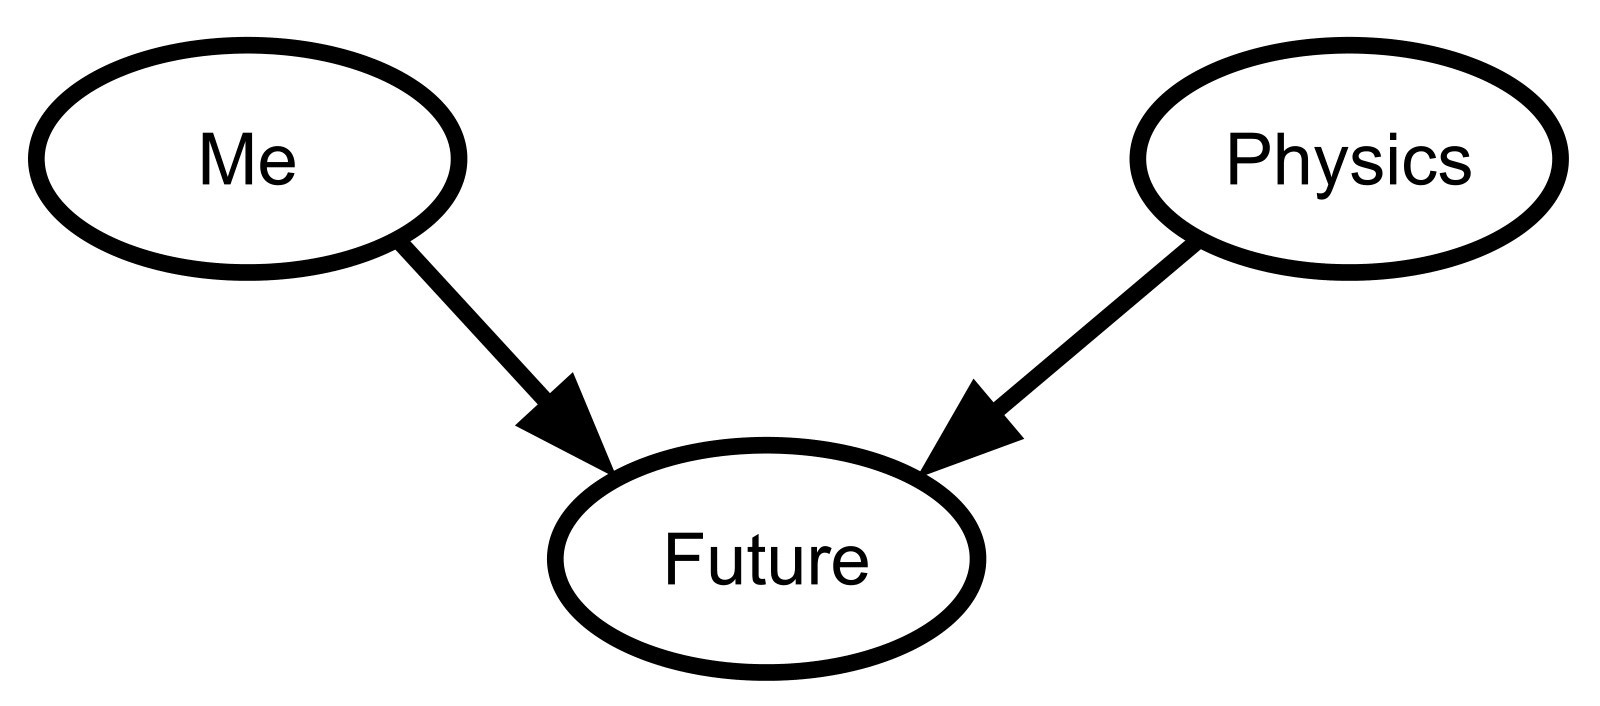
\includegraphics[scale=0.25]{Rationality20From20AI20to20Zombies2020Eliezer20Yudkowsky-img313.jpg}
 
\par}


\bigskip

{
\ \ \ ~}

{
\ \ \ Here we see the causes ``Me''
and ``Physics,'' competing to
determine the state of the
``Future'' effect. If the
``Future'' is fully determined by
``Physics,'' then obviously there is
no room for it to be affected by
``Me.''}

{
\ \ \ This causal network is not an explicit philosophical belief.
It's implicit---a background representation of the
brain, controlling which philosophical arguments seem
``reasonable.'' It just seems like
the way things \textit{are}.}

{
\ \ \ Every now and then, another neuroscience press release appears,
claiming that, because researchers used an fMRI to spot the brain doing
something-or-other during a decision process,
\textit{it's not you who chooses, it's
your brain}.}

{
\ \ \ Likewise that old chestnut, ``Reductionism
undermines rationality itself. Because then, every time you said
something, it wouldn't be the result of
\textit{reasoning} about the evidence---it would be merely quarks
bopping around.''}

{
\ \ \ Of course the actual diagram should be:}

{
\ \ \ ~}

{\centering
\ \ \  
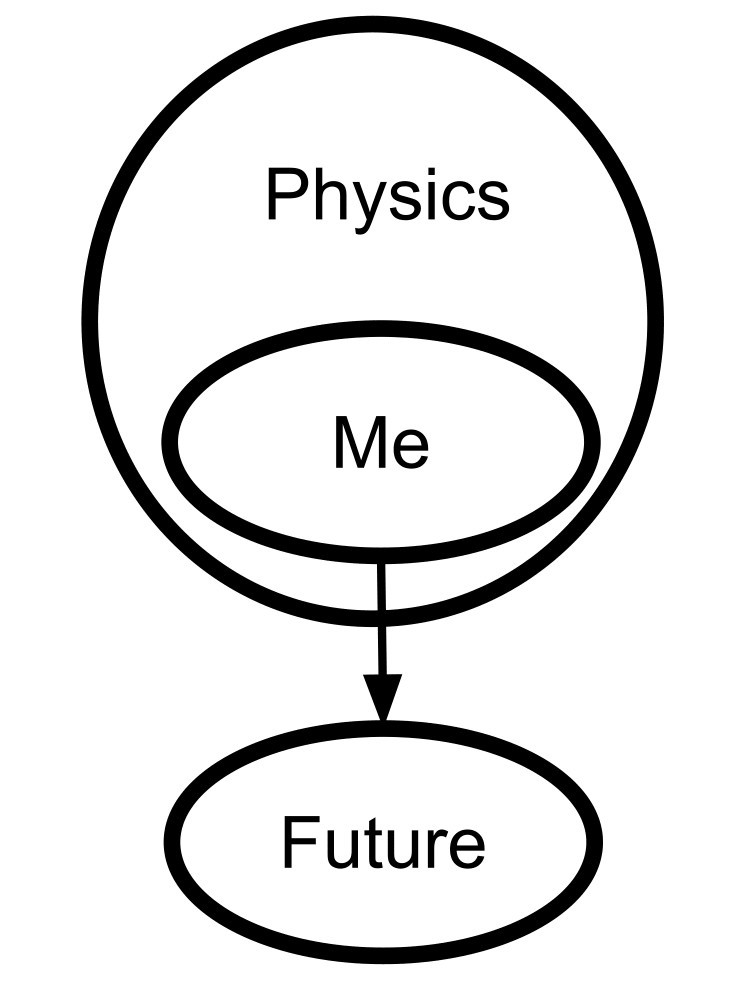
\includegraphics[scale=0.25]{Rationality20From20AI20to20Zombies2020Eliezer20Yudkowsky-img314.jpg}
 
\par}


\bigskip

{
\ \ \ ~}

{
\ \ \ Or better yet:}

{
\ \ \ ~}

{\centering
\ \ \  
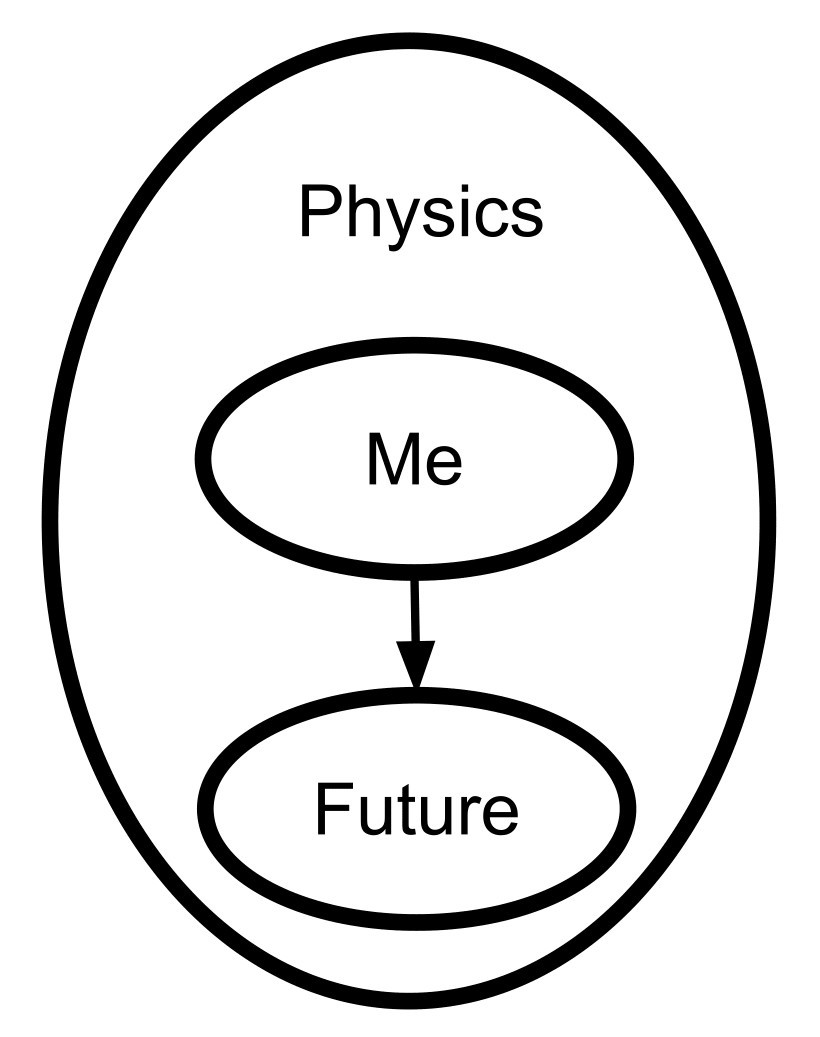
\includegraphics[scale=0.25]{Rationality20From20AI20to20Zombies2020Eliezer20Yudkowsky-img315.jpg}
 
\par}


\bigskip

{
\ \ \ ~}

{
\ \ \ Why is this not obvious? Because there are many levels of
organization that separate our models of our thoughts---our emotions,
our beliefs, our agonizing indecisions, and our final choices---from
our models of electrons and quarks.}

{
\ \ \ We can \textit{intuitively} visualize that a hand is made of
fingers (and thumb and palm). To ask whether it's
\textit{really} our hand that picks something up, or \textit{merely}
our fingers, thumb, and palm, is transparently a wrong question.}

{
\ \ \ But the gap between physics and cognition cannot be crossed by
direct visualization. No one can \textit{visualize} atoms making up a
person, the way they can see fingers making up a hand.}

{
\ \ \ And so it requires \textit{constant vigilance} to maintain your
perception of yourself as an entity \textit{within physics}.}

{
\ \ \ This vigilance is one of the great keys to philosophy, like the
Mind Projection Fallacy. You will recall that it is this point which I
nominated as having tripped up the quantum physicists who failed to
imagine macroscopic decoherence; they did not think to apply the laws
to \textit{themselves}.}

{
\ \ \ Beliefs, desires, emotions, morals, goals, imaginations,
anticipations, sensory perceptions, fleeting wishes, ideals,
temptations .~.~. You might call this the ``surface
layer'' of the mind, the parts-of-self that people
can see even without science. If I say, ``It is not
\textit{you} who determines the future, it is your \textit{desires,
plans, and actions} that determine the future,'' you
can readily see the part-whole relations. It is immediately visible,
like fingers making up a hand. There are other part-whole relations all
the way down to physics, but they are not immediately visible.}

{
\ \ \ ``Compatibilism'' is the
philosophical position that ``free
will'' can be intuitively and satisfyingly defined in
such a way as to be compatible with deterministic physics.
``Incompatibilism'' is the position
that free will and determinism are incompatible.}

{
\ \ \ My position might perhaps be called
``Requiredism.'' When agency,
choice, control, and moral responsibility are cashed out in a sensible
way, they \textit{require} determinism---at least some patches of
determinism within the universe. If you choose, and plan, and act, and
bring some future into being, in accordance with your desire, then all
this requires a lawful sort of reality; you cannot do it amid utter
chaos. There must be order over at least those parts of reality that
are being controlled by you. \textit{You} are within physics, and so
you/physics have determined the future. If it were not determined by
physics, it could not be determined by you.}

{
\ \ \ Or perhaps I should say, ``If the future were not
determined by reality, it could not be determined by
you,'' or ``If the future were not
determined by something, it could not be determined by
you.'' You don't need neuroscience or
physics to push naive definitions of free will into incoherence. If the
mind were not embodied in the brain, it would be embodied in something
else; there would be \textit{some real thing} that was a mind. If the
future were not determined by physics, it would be determined by
\textit{something}, some law, some order, some grand reality that
included you within it.}

{
\ \ \ But if the laws of physics control us, then how can we be said to
control ourselves?}

{
\ \ \ Turn it around: If the laws of physics did \textit{not} control
us, how could we possibly control ourselves?}

{
\ \ \ How could thoughts judge other thoughts, how could emotions
conflict with each other, how could one course of action appear best,
how could we pass from uncertainty to certainty about our own plans, in
the midst of utter chaos?}

{
\ \ \ If we were not in reality, where could we be?}

{
\ \ \ The future is determined by physics. What kind of physics? The
kind of physics that includes the actions of human beings.}

{
\ \ \ People's choices are determined by physics. What
kind of physics? The kind of physics that includes weighing decisions,
considering possible outcomes, judging them, being tempted, following
morals, rationalizing transgressions, trying to do better .~.~.}

{
\ \ \ There is no point where a quark swoops in from Pluto and overrides
all this.}

{
\ \ \ The thoughts of your decision process are all \textit{real}, they
are all \textit{something}. But a thought is too big and complicated to
be an atom. So thoughts are made of smaller things, and our name for
the stuff that stuff is made of is
``physics.''}

{
\ \ \ Physics underlies our decisions and includes our decisions. It
does not explain them \textit{away}.}

{
\ \ \ Remember, physics adds up to normality; it's your
cognitive algorithms that generate confusion.}

{\centering
\ \ \ \ ~
\par}

{\centering
\ \ \ *
\par}

\mysection{Many Worlds, One Best Guess}

{
\ \ \ If you look at many microscopic physical phenomena---a photon, an
electron, a hydrogen atom, a laser---and a million other known
experimental setups---it is possible to come up with simple laws that
seem to govern all small things (so long as you don't
ask about gravity). These laws govern the evolution of a highly
abstract and mathematical object that I've been calling
the ``amplitude distribution,'' but
which is more widely referred to as the
``wavefunction.'' }

{
\ \ \ Now there are gruesome questions about the proper generalization
that covers all these tiny cases. Call an object
``grue'' if it appears green before
January 1, 2020 and appears blue thereafter. If all emeralds examined
so far have appeared green, is the proper generalization,
``Emeralds are green'' or
``Emeralds are grue''?}

{
\ \ \ The answer is that the proper generalization is
``Emeralds are green.''
I'm not going to go into the arguments at the moment.
It is not the subject of this essay, and the obvious answer in this
case happens to be correct. The true Way is not stupid: however clever
you may be with your logic, it should finally arrive at the right
answer rather than a wrong one.}

{
\ \ \ In a similar sense, the \textit{simplest} generalizations that
would cover observed \textit{microscopic} phenomena alone take the form
of ``All electrons have spin 1/2''
and not ``All electrons have spin 1/2 before January
1, 2020'' or ``All electrons have
spin 1/2 unless they are part of an entangled system that weighs more
than 1 gram.''}

{
\ \ \ When we turn our attention to macroscopic phenomena, our sight is
obscured. We cannot experiment on the wavefunction of a human in the
way that we can experiment on the wavefunction of a hydrogen atom. In
no case can you actually read off the wavefunction with a little
quantum scanner. But in the case of, say, a human, the size of the
entire organism defeats our ability to perform precise calculations or
precise experiments---we cannot confirm that the quantum equations are
being obeyed \textit{in precise detail.}}

{
\ \ \ We know that phenomena commonly thought of as
``quantum'' do not just disappear
when many microscopic objects are aggregated. Lasers put out a flood of
coherent photons, rather than, say, doing something completely
different. Atoms have the chemical characteristics that quantum theory
says they should, enabling them to aggregate into the stable molecules
making up a human.}

{
\ \ \ So in one sense, we have a great deal of evidence that quantum
laws are aggregating to the macroscopic level without too much
difference. Bulk chemistry still works.}

{
\ \ \ But we cannot directly verify that the particles making up a human
have an aggregate wavefunction that behaves \textit{exactly} the way
the simplest quantum laws say. Oh, we know that molecules and atoms
don't disintegrate, we know that macroscopic mirrors
still reflect from the middle. We can get \textit{many} high-level
predictions from the assumption that the microscopic and the
macroscopic are governed by the same laws, and every prediction tested
has come true.}

{
\ \ \ But if someone were to claim that the macroscopic quantum picture
differs from the microscopic one in some as-yet-untestable
detail---something that only shows up at the unmeasurable 20th decimal
place of microscopic interactions, but aggregates into something bigger
for macroscopic interactions---well, we can't
\textit{prove} they're wrong. It is
Occam's Razor that says, ``There are
zillions of new fundamental laws you could postulate in the 20th
decimal place; why are you even \textit{thinking} about this
one?''}

{
\ \ \ If we calculate using the simplest laws which govern all known
cases, we find that humans end up in states of quantum superposition,
just like photons in a superposition of reflecting from and passing
through a half-silvered mirror. In the Schrödinger's
Cat setup, an unstable atom goes into a superposition of
disintegrating, and not-disintegrating. A sensor, tuned to the atom,
goes into a superposition of triggering and not-triggering. (Actually,
the superposition is now a joint state of [atom-disintegrated
{\texttimes} sensor-triggered] + [atom-stable {\texttimes}
sensor-not-triggered].) A charge of explosives, hooked up to the
sensor, goes into a superposition of exploding and not exploding; a cat
in the box goes into a superposition of being dead and alive; and a
human, looking inside the box, goes into a superposition of throwing up
and being calm. The same law at all levels.}

{
\ \ \ Human beings who interact with superposed systems will themselves
evolve into superpositions. But the brain that sees the exploded cat,
and the brain that sees the living cat, will have many neurons firing
differently, and hence many \textit{many} particles in different
positions. They are very distant in the configuration space, and will
communicate to an exponentially infinitesimal degree. Not the 30th
decimal place, but the 10\textsuperscript{30}th decimal place. No
particular mind, no particular cognitive causal process, sees a blurry
superposition of cats.}

{
\ \ \ The fact that ``you'' only seem
to see the cat alive, \textit{or} the cat dead, is exactly what the
simplest quantum laws predict. So we have no reason to believe, from
our experience so far, that the quantum laws are in any way different
at the macroscopic level than the microscopic level.}

{
\ \ \ And physicists have verified superposition at steadily larger
levels. Apparently an effort is currently underway to test
superposition in a 50-micron object, larger than most neurons.}

{
\ \ \ The existence of other versions of ourselves, and indeed other
Earths, is not supposed \textit{additionally.} We are simply supposing
that the same laws govern at all levels, having no reason to suppose
differently, and all experimental tests having succeeded so far. The
existence of other decoherent Earths is a \textit{logical consequence}
of the simplest generalization that fits all known facts. If you think
that Occam's Razor says that the other worlds are
``unnecessary entities'' being
multiplied, then you should check the probability-theoretic math; that
is just not how Occam's Razor works.}

{
\ \ \ Yet there is one particular puzzle that seems odd in trying to
extend microscopic laws universally, including to superposed humans:}

{
\ \ \ \textit{If} we try to get probabilities by counting the number of
distinct observers, then there is no \textit{obvious} reason why the
integrated squared modulus of the wavefunction should correlate with
statistical experimental results. There is no known reason for the Born
probabilities, and it even seems that, a priori, we would expect a
50/50 probability of any binary quantum experiment going both ways, if
we just counted observers.}

{
\ \ \ Robin Hanson suggests that if exponentially tinier-than-average
decoherent blobs of amplitude
(``worlds'') are interfered with by
exponentially tiny leakages from larger blobs, we will get the Born
probabilities back out. I consider this an interesting possibility,
because it is so normal.}

{
\ \ \ (I myself have had recent thoughts along a different track: If I
try to count observers the obvious way, I get strange-seeming results
in general, not just in the case of quantum physics. If, for example, I
split my brain into a trillion similar parts, conditional on winning
the lottery while anesthetized; allow my selves to wake up and perhaps
differ to small degrees from each other; and then merge them all into
one self again; then counting observers the obvious way says I should
be able to make myself win the lottery (if I can split my brain and
merge it, as an uploaded mind might be able to do).}

{
\ \ \ In this connection, I find it very interesting that the Born rule
does \textit{not} have a split-remerge problem. Given unitary quantum
physics, Born's rule is the \textit{unique} rule that
prevents ``observers'' from having
psychic powers---which doesn't \textit{explain}
Born's rule, but is certainly an \textit{interesting
fact}. Given Born's rule, even splitting and remerging
worlds would still lead to consistent probabilities. Maybe physics uses
better anthropics than I do!}

{
\ \ \ Perhaps I should take my cues from physics, instead of trying to
reason it out a priori, and see where that leads me? But I have not
been led anywhere \textit{yet}, so this is hardly an
``answer.'')}

{
\ \ \ Wallace, Deutsch, and others try to derive Born's
Rule from decision theory. I am rather suspicious of this, because it
seems like there is a component of ``What happens to
me?'' that I cannot alter by modifying my utility
function. Even if I didn't \textit{care} at all about
worlds where I didn't win a quantum lottery, it still
seems to me that there is a sense in which I would
``mostly'' wake up in a world where
I didn't win the lottery. It is this that I think needs
explaining.}

{
\ \ \ The point is that many hypotheses about the Born probabilities
have been proposed. Not as many as there should be, because the mystery
was falsely marked ``solved'' for a
long time. But still, there have been many proposals.}

{
\ \ \ There is legitimate hope of a solution to the Born puzzle without
new fundamental laws. Your world does not split into exactly two new
subprocesses on the exact occasion when you see
``ABSORBED'' or
``TRANSMITTED'' on the LCD screen of
a photon sensor. We are constantly being superposed and decohered, all
the time, sometimes along continuous dimensions---though brains are
digital and involve whole neurons firing, and fire/not-fire would be an
extremely decoherent state even of a \textit{single} neuron .~.~. There
would seem to be room for \textit{something} unexpected to account for
the Born statistics---a better understanding of the anthropic weight of
observers, or a better understanding of the brain's
superpositions---without new fundamentals.}

{
\ \ \ We cannot rule out, though, the possibility that a new fundamental
law is involved in the Born statistics.}

{
\ \ \ As Jess Riedel puts it:}

{
\ \ \ If there's one lesson we can take from the history
of physics, it's that everytime new experimental
``regimes'' are probed (e.g. large
velocities, small sizes, large mass densities, large energies),
phenomena are observed which lead to new theories (Special Relativity,
quantum mechanics, General Relativity, and the Standard Model,
respectively).}

{
\ \ \ ``Every time'' is too strong. A
nitpick, yes, but also an important point: you can't
just \textit{assume} that any particular law will fail in a new regime.
But it's possible that a new fundamental law is
involved in the Born statistics, and that this law manifests only in
the 20th decimal place at microscopic levels (hence being undetectable
so far) while aggregating to have substantial effects at macroscopic
levels.}

{
\ \ \ Could there be some law, as yet undiscovered, that causes there to
be only \textit{one} world?}

{
\ \ \ This is a shocking notion; it implies that all our twins in the
other worlds---all the different versions of ourselves that are
constantly split off, not just by human researchers doing quantum
measurements, but by ordinary entropic processes---are actually
\textit{gone}, leaving us alone! This version of Earth would be the
\textit{only} version that exists in local space! If the inflationary
scenario in cosmology turns out to be wrong, and the topology of the
universe is both finite and relatively small---so that Earth does not
have the distant duplicates that would be implied by an exponentially
vast universe---then this Earth could be the only Earth that exists
\textit{anywhere}, a rather unnerving thought!}

{
\ \ \ But it is dangerous to focus too much on specific hypotheses that
you have no specific reason to think about. This is the same root error
of the Intelligent Design folk, who pick any random puzzle in modern
genetics, and say, ``See, God must have done
it!'' Why ``God,''
rather than a zillion other possible explanations?---which you would
have thought of long before you postulated divine intervention, if not
for the fact that you secretly started out already knowing the answer
you wanted to find.}

{
\ \ \ You shouldn't even \textit{ask},
``Might there only be one world?''
but instead just go ahead and do physics, and raise that
\textit{particular} issue only if new evidence demands it.}

{
\ \ \ Could there be some as-yet-unknown fundamental law, that gives the
universe a privileged center, which happens to coincide with
Earth---thus proving that Copernicus was wrong all along, and the Bible
right?}

{
\ \ \ Asking \textit{that particular} question---rather than a zillion
other questions in which the center of the universe is Proxima
Centauri, or the universe turns out to have a favorite pizza topping
and it is pepperoni---betrays your hidden agenda. And though an
unenlightened one might not realize it, giving the universe a
privileged center \textit{that follows Earth around through space}
would be rather difficult to do with any \textit{mathematically simple}
fundamental law.}

{
\ \ \ So too with asking whether there might be only one world. It
betrays a sentimental attachment to human intuitions already proven
wrong. The wheel of science turns, but it doesn't turn
\textit{backward}.}

{
\ \ \ We have specific reasons to be highly suspicious of the notion of
only one world. The notion of ``one
world'' exists on a higher level of organization,
like the location of Earth in space; on the quantum level there are no
firm boundaries (though brains that differ by entire neurons firing are
certainly decoherent). How would a \textit{fundamental} physical law
identify one \textit{high-level} world?}

{
\ \ \ \textit{Much worse}, any physical scenario in which there was a
\textit{single} surviving world, so that any measurement had only a
\textit{single} outcome, would violate Special Relativity.}

{
\ \ \ If the same laws are true at all levels---i.e., if many-worlds is
correct---then when you measure one of a pair of entangled polarized
photons, you end up in a world in which the photon is polarized, say,
up-down, and alternate versions of you end up in worlds where the
photon is polarized left-right. From your perspective before doing the
measurement, the probabilities are 50/50. Light-years away, someone
measures the other photon at a 20\textsuperscript{°} angle to your own
basis. From their perspective, too, the probability of getting either
immediate result is 50/50---they maintain an invariant state of
generalized entanglement with your faraway location, no matter what you
do. But when the two of you meet, years later, your probability of
meeting a friend who got the \textit{same} result is 11.6\%, rather
than 50\%.}

{
\ \ \ If there is only one global world, then there is only a single
outcome of any quantum measurement. Either you measure the photon
polarized up-down, or left-right, but not both. Light-years away,
someone else's probability of measuring the photon
polarized similarly in a 20\textsuperscript{°} rotated basis actually
\textit{changes} from 50/50 to 11.6\%.}

{
\ \ \ You cannot possibly interpret this as a case of merely revealing
properties that were already there; this is ruled out by
Bell's Theorem. There does not seem to be any possible
consistent view of the universe in which both quantum measurements have
a single outcome, and yet both measurements are predetermined, neither
influencing the other. Something has to actually \textit{change},
faster than light.}

{
\ \ \ And this would appear to be a fully general objection, not just to
collapse theories, but to any possible theory that gives us one global
world! There is no consistent view in which measurements have single
outcomes, but are locally determined (even locally randomly
determined). Some mysterious influence has to cross a spacelike gap.}

{
\ \ \ This is not a trivial matter. You cannot save yourself by waving
your hands and saying, ``the influence travels
backward in time to the entangled photons' creation,
then forward in time to the other photon, so it never actually crosses
a spacelike gap.'' (This view has been seriously put
forth, which gives you some idea of the magnitude of the paradox
implied by one global world!) One measurement has to change the other,
so which measurement happens \textit{first}? Is there a global space of
simultaneity? You can't have both measurements happen
``first'' because under
Bell's Theorem, there's no way local
information could account for observed results, etc.}

{
\ \ \ Incidentally, this experiment has already been performed, and if
there is a mysterious influence it would have to travel six million
times as fast as light in the reference frame of the Swiss Alps. Also,
the mysterious influence has been experimentally shown not to care if
the two photons are measured in reference frames which would cause each
measurement to occur ``before the
other.''}

{
\ \ \ Special Relativity seems counterintuitive to us humans---like an
arbitrary speed limit, which you could get around by going backward in
time, and then forward again. A law you could escape prosecution for
violating, if you managed to hide your crime from the authorities.}

{
\ \ \ But what Special Relativity really says is that human intuitions
about space and time are simply wrong. There \textit{is} no global
``now,'' there \textit{is} no
``before'' or
``after'' across spacelike gaps. The
ability to \textit{visualize} a single global world, \textit{even in
principle,} comes from not getting Special Relativity on a gut level.
Otherwise it would be obvious that physics proceeds locally with
invariant states of distant entanglement, and the requisite information
is simply \textit{not} \textit{locally present} to support a
\textit{globally single world}.}

{
\ \ \ It might be that this seemingly impeccable logic is flawed---that
my application of Bell's Theorem and relativity to rule
out any single global world contains some hidden assumption of which I
am unaware---}

{
\ \ \ {}---but consider the burden that a single-world theory must now
shoulder! There is absolutely no reason \textit{in the first place} to
suspect a global single world; this is just \textit{not what current
physics says!} The global single world is an ancient human intuition
that was \textit{disproved}, like the idea of a universal absolute
time. The superposition principle is visible even in half-silvered
mirrors; experiments are verifying the disproof at steadily larger
levels of superposition---but above all there is \textit{no longer any
reason} to \textit{privilege the hypothesis} of a global single world.
The ladder has been yanked out from underneath that human intuition.}

{
\ \ \ There is no experimental evidence that the macroscopic world is
single (we already know the microscopic world is superposed). And the
prospect necessarily either violates Special Relativity, or takes an
even more miraculous-seeming leap and violates seemingly impeccable
logic. The latter, of course, being much more plausible in practice.
But it isn't really \textit{that} plausible in an
absolute sense. \textit{Without experimental evidence,} it is generally
a \textit{bad sign} to have to postulate arbitrary logical miracles.}

{
\ \ \ As for quantum non-realism, it appears to me to be nothing more
than a Get Out of Jail Free card.
``It's okay to violate Special
Relativity because none of this is real anyway!'' The
equations cannot reasonably be hypothesized to deliver such excellent
predictions \textit{for literally no reason.} Bell's
Theorem rules out the obvious possibility that quantum theory
represents imperfect knowledge of something locally deterministic.}

{
\ \ \ Furthermore, macroscopic decoherence gives us a perfectly
\textit{realistic} understanding of what is going on, in which the
equations deliver such good predictions because they mirror reality.
And so the idea that the quantum equations are just
``meaningless,'' and therefore it is
okay to violate Special Relativity, so we can have one global world
after all, is not \textit{necessary}. To me, quantum non-realism
appears to be a huge bluff built around semantic stopsigns like
``Meaningless!''}

{
\ \ \ It is not quite safe to say that the existence of multiple Earths
is as well-established as any other truth of science. The existence of
quantum other worlds is not so well-established as the existence of
trees, which most of us can personally observe.}

{
\ \ \ Maybe there is something in that 20th decimal place, which
aggregates to something bigger in macroscopic events. Maybe
there's a loophole in the seemingly iron logic which
says that any single global world must violate Special Relativity,
because the information to support a single global world is not locally
available. And maybe the Flying Spaghetti Monster is just messing with
us, and the world we know is a lie.}

{
\ \ \ So all we can say about the existence of multiple Earths, is that
it is as rationally probable as e.g. the statement that spinning black
holes do not violate conservation of angular momentum. We have
extremely fundamental reasons, having to do with the rotational
symmetry of space, to suspect that conservation of angular momentum is
built into the underlying nature of physics. And we have no specific
reason to suspect this \textit{particular} violation of our old
generalizations in a higher-energy regime.}

{
\ \ \ But we haven't actually checked conservation of
angular momentum for rotating black holes---so far as I know. (And as I
am talking here about rational guesses in states of partial knowledge,
the point is exactly the same if the observation has been made and I do
not know it yet.) And black holes are a more massive regime. So the
obedience of black holes is not \textit{quite} as assured as that my
toilet conserves angular momentum while flushing, which come to think,
I haven't checked either .~.~.}

{
\ \ \ Yet if you make the \textit{mistake} of thinking too hard about
this one particular possibility, instead of zillions of other
possibilities---and especially if you don't understand
the fundamental reason \textit{why} angular momentum is
conserved---then it may start seeming more and more plausible that
``spinning black holes violate conservation of angular
momentum,'' as you think of more and more vaguely
plausible-sounding reasons it \textit{could} be true.}

{
\ \ \ But the rational probability is pretty damned small.}

{
\ \ \ Likewise the rational probability that there is only one Earth.}

{
\ \ \ I mention this to explain my habit of talking as if many-worlds is
an obvious fact. Many-worlds \textit{is} an obvious fact, if you have
all your marbles lined up correctly (understand very basic quantum
physics, know the formal probability theory of Occam's
Razor, understand Special Relativity, etc.) It is in fact considerably
\textit{more} obvious to me than the proposition that spinning black
holes should obey conservation of angular momentum.}

{
\ \ \ The only reason why many-worlds is not universally acknowledged as
a direct prediction of physics which requires magic to violate, is that
a contingent accident of our Earth's scientific history
gave an entrenched academic position to a phlogiston-like theory that
had an unobservable faster-than-light magical
``collapse'' devouring all other
worlds. And many academic physicists do not have a mathematical grasp
of Occam's Razor, which is the usual method for ridding
physics of invisible angels. So when they encounter many-worlds and it
conflicts with their (undermined) intuition that only one world exists,
they say, ``Oh, that's multiplying
entities''---which is just flatly wrong as
probability theory---and go on about their daily lives.}

{
\ \ \ I am not in academia. I am not constrained to bow and scrape to
some senior physicist who hasn't grasped the obvious,
but who will be reviewing my journal articles. I need have no fear that
I will be rejected for tenure on account of scaring my students with
``science-fiction tales of other
Earths.'' If \textit{I} can't speak
plainly, who can?}

{
\ \ \ So let me state then, very clearly, on behalf of any and all
physicists out there who dare not say it themselves: Many-worlds
\textit{wins outright} given our current state of evidence. There is no
more reason to postulate a single Earth, than there is to postulate
that two colliding top quarks would decay in a way that violates
Conservation of Energy. It takes more than an unknown fundamental law;
it takes magic.}

{
\ \ \ \textit{The debate should already be over. It should have been
over fifty years ago. The state of evidence is too lopsided to justify
further argument. There is no balance in this issue. There is no
rational controversy to teach. The laws of probability theory are laws,
not suggestions; there is no flexibility in the best guess given this
evidence. Our children will look back at the fact that we were STILL
ARGUING about this in the early twenty-first century, and correctly
deduce that we were nuts.}}

{
\ \ \ We have embarrassed our Earth long enough by failing to see the
obvious. So for the honor of my Earth, I write as if the existence of
many-worlds were an established fact, because it \textit{is.} The only
question now is how long it will take for the people of this world to
update.}

{\centering
\ \ \ \ ~
\par}

{\centering
\ \ \ *
\par}

\chapter{Science and Rationality}

\mysection{The Failures of Eld Science}

{
\ \ \ This time there were no robes, no hoods, no masks. Students were
expected to become friends, and allies. And everyone knew why you were
in the classroom. It would have been pointless to pretend you
weren't in the Conspiracy. }

{
\ \ \ Their \textit{sensei} was Jeffreyssai, who might have been the
best of his era, in his era. His students were either the most
promising learners, or those whom the \textit{beisutsukai} saw
political advantage in molding.}

{
\ \ \ Brennan fell into the latter category, and knew it. Nor had he
hesitated to use his Mistress's name to open doors. You
used every avenue available to you, in seeking knowledge; that was
respected here.}

{
\ \ \ ``---for over thirty years,''
Jeffreyssai said. ``Not one of them saw it; not
Einstein, not Schrödinger, not even von Neumann.'' He
turned away from his sketcher, and toward the classroom.
``I pose to you to the question: How did they
fail?''}

{
\ \ \ The students exchanged quick glances, a calculus of mutual risk
between the wary and the merely baffled. Jeffreyssai was known to play
games.}

{
\ \ \ Finally Hiriwa-called-the-Black leaned forward, jangling slightly
as her equation-carved bracelets shifted on her ankles.
``By your years given, \textit{sensei}, this was two
hundred and fifty years after Newton. Surely, the scientists of that
era must have grokked the concept of a universal
law.''}

{
\ \ \ ``Knowing the universal law of
gravity,'' said the student Taji, from a nearby seat,
``is not the same as understanding the concept
\textit{of} a universal law.'' He was one of the
promising ones, as was Hiriwa.}

{
\ \ \ Hiriwa frowned. ``No .~.~. it was said that
Newton had been praised \textit{for} discovering the first universal.
Even in his own era. So it was known.'' Hiriwa
paused. ``But Newton himself would have been gone. Was
there a \textit{religious} injunction against proposing further
universals? Did they refrain out of respect for Newton, or were they
waiting for his \textit{ghost} to speak? I am not clear on how Eld
science was motivated---''}

{
\ \ \ ``No,'' murmured Taji, a laugh
in his voice, ``you really, \textit{really}
aren't.''}

{
\ \ \ Jeffreyssai's expression was kindly.
``Hiriwa, it wasn't religion, and it
wasn't lead in the drinking water, and they
didn't all have Alzheimer's, and they
weren't sitting around all day reading webcomics.
Forget the catalogue of horrors out of ancient times. Just think in
terms of cognitive errors. What could Eld science have been
\textit{thinking} wrong?''}

{
\ \ \ Hiriwa sat back with a sigh. ``\textit{Sensei}, I
truly cannot imagine a snafu that would do
\textit{that}.''}

{
\ \ \ ``It wouldn't be just
\textit{one} mistake,'' Taji corrected her.
``As the saying goes: Mistakes don't
travel alone; they hunt in packs.''}

{
\ \ \ ``But the \textit{entire} human
species?'' said Hiriwa. ``Thirty
\textit{years}?''}

{
\ \ \ ``It wasn't the entire human
species, Hiriwa,'' said Styrlyn. He was one of the
older-looking students, wearing a short beard speckled in gray.
``Maybe one in a hundred thousand could have written
out Schrödinger's Equation from memory. So that would
have been their first and primary error---failure to concentrate their
forces.''}

{
\ \ \ ``\textit{Spare us the
propaganda!}'' Jeffreyssai's gaze was
suddenly fierce. ``You are not here to proselytize for
the Cooperative Conspiracy, my lord politician! Bend not the truth to
make your points! I believe your Conspiracy has a phrase:
`Comparative advantage.' Do you
\textit{really} think that it would have helped to call in the whole
human species, as it existed at that time, to debate quantum
physics?''}

{
\ \ \ Styrlyn didn't flinch. ``Perhaps
not, \textit{sensei},'' he said.
``But if you are to compare that era to this one, it
is a consideration.''}

{
\ \ \ Jeffreyssai moved his hand flatly through the air; the
maybe-gesture he used to dismiss an argument that was true but not
relevant. ``It is not what I would call a
\textit{primary} mistake. The puzzle should not have required a billion
physicists to solve.''}

{
\ \ \ ``I can think of more \textit{specific} ancient
horrors,'' said Taji. ``Spending all
day writing grant proposals. Teaching undergraduates who would rather
be somewhere else. Needing to publish thirty papers a year to get
tenure .~.~.''}

{
\ \ \ ``But we are not speaking of only the
lower-status scientists,'' said Yin; she wore a
slightly teasing grin. ``It was said of Schrödinger
that he retired to a villa for a month, with his mistress to provide
inspiration, and emerged with his eponymous equation. We consider it a
famous historical success of our methodology. Some Eld physicists
\textit{did} understand how to focus their mental energies; and would
have been senior enough to do so, had they chose.''}

{
\ \ \ ``True,'' Taji said.
``In the end, administrative burdens are only a
generic obstacle. Likewise such answers as, `They were
not trained in probability theory, and did not know of cognitive
biases.' Our sensei seems to desire some more specific
reply.''}

{
\ \ \ Jeffreyssai lifted an eyebrow encouragingly.
``Don't dismiss your line of thought
so quickly, Taji; it begins to be relevant. What kind of system would
create administrative burdens on its own people?''}

{
\ \ \ ``A system that failed to support its people
adequately,'' said Styrlyn. ``One
that failed to value their work.''}

{
\ \ \ ``Ah,'' said Jeffreyssai.
``But there is a student who has not yet spoken.
\textit{Brennan?}''}

{
\ \ \ Brennan didn't jump. He deliberately waited just
long enough to show he wasn't scared, and then said,
``Lack of pragmatic motivation,
sensei.''}

{
\ \ \ Jeffreyssai smiled slightly.
``Expand.''}

{
\ \ \ \textit{What kind of system would create administrative burdens on
its own people?}, their \textit{sensei} had asked them. The other
students were pursuing their own lines of thought. Brennan, hanging
back, had more attention to spare for his teacher's few
hints. Being the beginner wasn't \textit{always} a
disadvantage---and he had been taught, long before the Bayesians took
him in, to take every available advantage.}

{
\ \ \ ``The Manhattan Project,''
Brennan said, ``was launched with a specific
\textit{technological} end in sight: a weapon of great power, in time
of war. But the error that Eld Science committed with respect to
quantum physics had no immediate consequences for their technology.
They were confused, but they had no desperate \textit{need} for an
answer. Otherwise the surrounding system would have removed all burdens
from their effort to solve it. Surely the Manhattan Project must have
done so---Taji? Do you know?''}

{
\ \ \ Taji looked thoughtful. ``Not \textit{all}
burdens---but I'm pretty sure they
weren't writing grant proposals in the middle of their
work.''}

{
\ \ \ ``So,'' Jeffreyssai said. He
advanced a few steps, stood directly in front of
Brennan's desk. ``You think Eld
scientists simply weren't trying hard enough. Because
their art had no military applications? A rather \textit{competitive}
point of view, I should think.''}

{
\ \ \ ``Not necessarily,'' Brennan
said calmly. ``Pragmatism is a virtue of rationality
also. A desired \textit{use} for a better quantum theory would have
helped the Eld scientists in many ways beyond just motivating them. It
would have given shape to their curiosity, and told them what
constituted success or failure.''}

{
\ \ \ Jeffreyssai chuckled slightly.
``Don't guess so hard what \textit{I}
might prefer to hear, Competitor. Your first statement came closer to
my hidden mark; your oh-so-Bayesian disclaimer fell wide .~.~. The
factor I had in mind, Brennan, was that Eld scientists thought it was
\textit{acceptable} to take thirty years to solve a problem. Their
entire social process of science was based on getting to the truth
\textit{eventually.} A wrong theory got discarded
\textit{eventually}{}---once the next generation of students grew up
familiar with the replacement. Work expands to fill the time allotted,
as the saying goes. But people can think important thoughts in far less
than thirty years, if they \textit{expect} speed of
themselves.'' Jeffreyssai suddenly slammed down a
hand on the arm of Brennan's chair.
``\textit{How long do you have to dodge a thrown
knife?}''}

{
\ \ \ ``Very little time, sensei!''}

{
\ \ \ ``\textit{Less than a second! Two opponents are
attacking you! How long do you have to guess who's more
dangerous?}''}

{
\ \ \ ``Less than a second,
sensei!''}

{
\ \ \ ``\textit{The two opponents have split up and are
attacking two of your girlfriends! How long do you have to decide which
one you truly love?}''}

{
\ \ \ ``Less than a second,
sensei!''}

{
\ \ \ ``\textit{A new argument shows your precious
theory is flawed! How long does it take you to change your
mind?}''}

{
\ \ \ ``Less than a second,
sensei!''}

{
\ \ \ ``\textit{WRONG! DON'T GIVE ME
THE WRONG ANSWER JUST BECAUSE IT FITS A CONVENIENT PATTERN AND I SEEM
TO EXPECT IT OF YOU!} How long does it really take,
Brennan?''}

{
\ \ \ Sweat was forming on Brennan's back, but he
stopped and actually thought about it---}

{
\ \ \ ``\textit{ANSWER, BRENNAN!}''}

{
\ \ \ ``\textit{No, sensei! I'm not
finished thinking, sensei! An answer would be premature!
Sensei!}''}

{
\ \ \ ``\textit{Very good! Continue! But
don't take thirty years!}''}

{
\ \ \ Brennan breathed deeply, reforming his thoughts. He finally said,
``Realistically, sensei, the best-case scenario is
that I would see the problem immediately; use the discipline of
suspending judgment; try to re-accumulate all the evidence before
continuing; and depending on how emotionally attached I had been to the
theory, use the crisis-of-belief technique to ensure I could genuinely
go either way. So at least five minutes and perhaps up to an
hour.''}

{
\ \ \ ``\textit{Good! You actually thought about it
that time! Think about it every time! Break patterns!} In the days of
Eld Science, Brennan, it was not uncommon for a grant agency to spend
six months reviewing a proposal. \textit{They permitted themselves the
time!} You are being graded on your \textit{speed}, Brennan! The
question is not whether you get there eventually! Anyone can find the
truth in five thousand years! You need to \textit{move
faster!}''}

{
\ \ \ ``\textit{Yes, sensei!}''}

{
\ \ \ ``Now, Brennan, have you just learned something
new?''}

{
\ \ \ ``Yes, sensei!''}

{
\ \ \ ``How long did it take you to learn this new
thing?''}

{
\ \ \ An arbitrary choice there .~.~. ``Less than a
minute, sensei, from the boundary that seems most
obvious.''}

{
\ \ \ ``Less than a minute,''
Jeffreyssai repeated. ``So, Brennan, how long do you
think it should take to solve a major scientific problem, if you are
not wasting any time?''}

{
\ \ \ Now there was a trapped question if Brennan had ever heard one.
There was no way to guess what time period Jeffreyssai had in
mind---what the \textit{sensei} would consider too long, or too short.
Which meant that the only way out was to just try for the genuine
truth; this would offer him the defense of honesty, little defense
though it was. ``One year,
sensei?''}

{
\ \ \ ``Do you think it could be done in one month,
Brennan? In a case, let us stipulate, where in principle you already
have enough experimental evidence to determine an answer, but not so
much experimental evidence that you can afford to make errors in
interpreting it.''}

{
\ \ \ Again, no way to guess which answer Jeffreyssai might \textit{want
.~.~.} ``One month seems like an unrealistically short
time to me, sensei.''}

{
\ \ \ ``A \textit{short time}?''
Jeffreyssai said incredulously. ``How many minutes in
thirty days? Hiriwa?''}

{
\ \ \ ``43,200, sensei,'' she
answered. ``If you assume sixteen-hour waking periods
and daily sleep, then 28,800 minutes.''}

{
\ \ \ ``Assume, Brennan, that it takes five whole
minutes to think an \textit{original} thought, rather than learning it
from someone else. Does even a major scientific problem require 5,760
distinct insights?''}

{
\ \ \ ``I confess, sensei,'' Brennan
said slowly, ``that I have never thought of it that
way before .~.~. but do you tell me that is \textit{truly} a realistic
level of productivity?''}

{
\ \ \ ``No,'' said Jeffreyssai,
``but neither is it realistic to think that a single
problem requires 5,760 insights. And yes, it has been
done.''}

{
\ \ \ Jeffreyssai stepped back, and smiled benevolently. Every student
in the room stiffened; they knew that smile. ``Though
none of you hit the particular answer that \textit{I} had in mind,
nonetheless your answers were as reasonable as mine. Except
Styrlyn's, I'm afraid. Even
Hiriwa's answer was not entirely wrong: the task of
proposing new theories was once considered a sacred duty reserved for
those of high status, there being a limited supply of problems in
circulation, at that time. But \textit{Brennan's}
answer is \textit{particularly} interesting, and I am minded to test
his theory of motivation.''}

{
\ \ \ \textit{Oh, hell,} Brennan said silently to himself. Jeffreyssai
was gesturing for Brennan to stand up before the class.}

{
\ \ \ When Brenann had risen, Jeffreyssai neatly seated himself in
Brennan's chair.}

{
\ \ \ ``Brennan-sensei,'' Jeffreyssai
said, ``you have five minutes to think of something
stunningly brilliant to say about the failure of Eld science on quantum
physics. As for the rest of us, our job will be to gaze at you
expectantly. I can only imagine how embarrassing it will be, should you
fail to think of anything good.''}

{
\ \ \ \textit{Bastard.} Brennan didn't say it aloud.
Taji's face showed a certain amount of sympathy;
Styrlyn held himself aloof from the game; but Yin was looking at him
with sardonic interest. Worse, Hiriwa \textit{was} gazing at him
expectantly, assuming that he would rise to the challenge. And
Jeffreyssai was gawking wide-eyed, waiting for the
guru's words of wisdom. \textit{Screw you, sensei.}}

{
\ \ \ Brennan didn't panic. It was very, very, very far
from being the scariest situation he'd ever faced. He
took a moment to decide how to think; then thought.}

{
\ \ \ At four minutes and thirty seconds, Brennan spoke. (There was an
art to such things; as long as you were doing it anyway, you might as
well make it look easy.)}

{
\ \ \ ``A woman of wisdom,'' Brennan
said, ``once told me that it is wisest to regard our
past selves as fools beyond redemption---to see the people we once were
as idiots entire. I do not necessarily say this myself; but it is what
she said to me, and there is more than a grain of truth in it. As long
as we are making excuses for the past, trying to make it look better,
\textit{respecting} it, we cannot make a clean break. It occurs to me
that the rule may be no different for human \textit{civilizations}. So
I tried looking back and considering the Eld scientists as simple
fools.''}

{
\ \ \ ``Which they were not,''
Jeffreyssai said.}

{
\ \ \ ``Which they were not,''
Brennan continued. ``In terms of raw intelligence,
they undoubtedly exceeded me. But it occurred to me that a difficulty
in seeing what Eld scientists did wrong, might have been in respecting
the ancient and legendary names too highly. And that did indeed produce
an insight.''}

{
\ \ \ ``Enough introduction,
Brennan,'' said Jeffreyssai. ``If
you found an insight, state it.''}

{
\ \ \ ``Eld scientists were not trained
.~.~.'' Brennan paused. ``No,
\textit{untrained} is not the concept. They were trained for the
\textit{wrong task.} At that time, there were no Conspiracies, no
secret truths; as soon as Eld scientists solved a major problem, they
published the solution to the world and each other. Truly scary and
confusing \textit{open problems} would have been in extremely rare
supply, and used up the moment they were solved. So it would not have
been possible to train Eld researchers \textit{to bring order out of
scientific chaos.} They would have been trained for something
else---I'm not sure what---''}

{
\ \ \ ``Trained to manipulate whatever science had
\textit{already} been discovered,'' said Taji.
``It was a difficult enough task for Eld teachers to
train their students to \textit{use existing knowledge}, or follow
already-known methodologies; that was all Eld science teachers aspired
to impart.''}

{
\ \ \ Brennan nodded. ``Which is a \textit{very}
different matter from creating new science of their own. The Eld
scientists, faced with problems of quantum theory, might never have
faced that kind of \textit{fear} before---the dismay of not knowing.
The Eld scientists might have seized on unsatisfactory answers
prematurely, because they were accustomed to working with a neat,
agreed-upon body of knowledge.''}

{
\ \ \ ``\textit{Good}, Brennan,''
murmured Jeffreyssai.}

{
\ \ \ ``But above all,'' Brennan
continued, ``an Eld scientist couldn't
have \textit{practiced} the actual problem the quantum scientists
faced---that of resolving a major confusion. It was something you did
once per lifetime if you were lucky, and as Hiriwa observed, Newton
would no longer have been around. So while the Eld physicists who
messed up quantum theory were not unintelligent, they were, in a strong
sense, \textit{amateurs}{}---ad-libbing the whole process of paradigm
shift.''}

{
\ \ \ ``And no probability theory,''
Hiriwa noted. ``So anyone who \textit{did} succeed at
the problem would have no idea what they'd just done.
They wouldn't be able to communicate it to anyone else,
except vaguely.''}

{
\ \ \ ``Yes,'' Styrlyn said.
``And it was only a handful of people who could tackle
the problem at all, with no training in doing so; those are the
physicists whose names have passed down to us. A handful of people,
making a handful of discoveries each. It would not have been enough to
sustain a community. Each Eld scientist tackling a new paradigm shift
would have needed to rediscover the rules from
scratch.''}

{
\ \ \ Jeffreyssai rose from Brenann's desk.
``Acceptable, Brennan; you surprise me, in fact. I
shall have to give further thought to this method of
yours.'' Jeffreyssai went to the classroom door, then
looked back. ``However, I did have in mind at least
one \textit{other} major flaw of Eld science, which none of you
suggested. I expect to receive a list of possible flaws tomorrow. I
expect the flaw I have in mind to be on the list. You have 480 minutes,
excluding sleep time. I see five of you here. The challenge does not
require more than 480 insights to solve, nor more than 96 insights in
series.''}

{
\ \ \ And Jeffreyssai left the room.}

{\centering
\ \ \ \ ~
\par}

{\centering
\ \ \ *
\par}

\mysection{The Dilemma: Science or Bayes?}

{
\ \ \ Eli: You are writing a lot about physics recently. Why?}

{\raggedleft
\ \ \ {}---Shane Legg (and several other people)
\par}


\bigskip

{
\ \ \ ~}

{
\ \ \ In light of your QM explanation, which to me sounds perfectly
logical, it seems \textit{obvious and normal} that many worlds is
overwhelmingly likely. It just seems almost too good to be true that
\textit{I} now get what plenty of genius quantum physicists still
can't. [ .~.~. ] Sure I can explain all that away, and
I still think you're right, I'm just
suspicious of myself for believing the first believable explanation I
met.}

{\raggedleft
\ \ \ {}---Recovering\_irrationalist
\par}


\bigskip

{
\ \ \ ~}

{
\ \ \ Recovering\_irrationalist, you've got no idea how
glad I was to see you post that comment.}

{
\ \ \ Of course I had more than just \textit{one} reason for spending
all that time writing about quantum physics. I like having lots of
hidden motives. It's the closest I can ethically get to
being a supervillain.}

{
\ \ \ But to give an example of a purpose I could \textit{only}
accomplish by discussing quantum physics .~.~.}

{
\ \ \ In physics, you can get absolutely clear-cut issues. Not in the
sense that the issues are trivial to explain. But if you try to apply
Bayes to healthcare, or economics, you may not be able to
\textit{formally} lay out what is the simplest hypothesis, or what the
evidence supports. But when I say ``macroscopic
decoherence is simpler than collapse'' it is actually
\textit{strict} simplicity; you could write the two hypotheses out as
computer programs and count the lines of code. Nor is the evidence
itself in dispute.}

{
\ \ \ I wanted a very clear example---\textit{Bayes says
``zig,'' this is a zag}{}---when it
came time to break your allegiance to Science.}

{
\ \ \ ``Oh, sure,'' you say,
``the physicists messed up the many-worlds thing, but
give them a break, Eliezer! No one ever claimed that the social process
of science was perfect. People are human; they make
mistakes.''}

{
\ \ \ But the physicists who refuse to adopt many-worlds
aren't disobeying the rules of Science.
They're \textit{obeying} the rules of Science.}

{
\ \ \ The tradition handed down through the generations says that a new
physics theory comes up with new experimental predictions that
distinguish it from the old theory. You perform the test, and the new
theory is confirmed or falsified. If it's confirmed,
you hold a huge celebration, call the newspapers, and hand out Nobel
Prizes for everyone; any doddering old emeritus professors who refuse
to convert are quietly humored. If the theory is disconfirmed, the lead
proponent publicly recants, and gains a reputation for honesty.}

{
\ \ \ This is not how things \textit{do} work in science; rather it is
how things are \textit{supposed} to work in Science.
It's the ideal to which all good scientists aspire.}

{
\ \ \ Now many-worlds comes along, and it doesn't seem
to make any new predictions relative to the old theory.
That's suspicious. And there's all
these other worlds, but you can't see them.
That's \textit{really} suspicious. It just
doesn't seem scientific.}

{
\ \ \ If you got as far as Recovering\_irrationalist---so that
many-worlds now seems perfectly logical, obvious and
normal---\textit{and} you also started out as a Traditional
Rationalist, then you should be able to switch back and forth between
the Scientific view and the Bayesian view, like a Necker Cube.}

{
\ \ \ So now put on your Science Goggles---you've still
got them around somewhere, right? Forget everything you know about
Kolmogorov complexity, Solomonoff induction or Minimum Message Lengths.
That's not part of the traditional training. You just
eyeball something to see how
``simple'' it looks. The word
``testable'' doesn't
conjure up a mental image of Bayes's Theorem governing
probability flows; it conjures up a mental image of being in a lab,
performing an experiment, and having the celebration (or public
recantation) afterward.}

{
\ \ \ \textit{Science-Goggles on}: The current quantum theory has passed
all experimental tests so far. Many-worlds doesn't make
any new testable predictions---the amazing new phenomena it predicts
are all hidden away where we can't see them. You can
get along fine without supposing the other worlds, and
that's just what you should do. The whole thing smacks
of science fiction. But it must be admitted that quantum physics is a
very deep and very confusing issue, and who knows what discoveries
might be in store? Call me when Many-worlds makes a testable
prediction.}

{
\ \ \ Science-Goggles off, Bayes-Goggles back on:}

{
\ \ \ \textit{Bayes-Goggles on}: The simplest quantum equations that
cover all known evidence don't have a special exception
for human-sized masses. There isn't even any reason to
ask that particular question. Next!}

{
\ \ \ Okay, so is this a problem we can fix in five minutes with some
duct tape and superglue?}

{
\ \ \ No.}

{
\ \ \ Huh? Why not just teach new graduating classes of scientists about
Solomonoff induction and Bayes's Rule?}

{
\ \ \ Centuries ago, there was a widespread idea that the Wise could
unravel the secrets of the universe just by thinking about them, while
to go out and \textit{look} at things was lesser, inferior, naive, and
would just delude you in the end. You couldn't trust
the way things \textit{looked}{}---only thought could be your guide.}

{
\ \ \ Science began as a rebellion against this Deep Wisdom. At the core
is the pragmatic belief that human beings, sitting around in their
armchairs trying to be Deeply Wise, just drift off into never-never
land. You couldn't trust your thoughts. You had to make
advance experimental predictions---predictions that no one else had
made before---run the test, and confirm the result. That was evidence.
Sitting in your armchair, thinking about what seemed reasonable .~.~.
would not be taken to \textit{prejudice} your theory, because Science
wasn't an idealistic belief about pragmatism, or
getting your hands dirty. It was, rather, the dictum that experiment
alone would decide. Only experiments could judge your theory---not your
nationality, or your religious professions, or the fact that
you'd invented the theory in your armchair. Only
experiments! If you sat in your armchair and came up with a theory that
made a novel prediction, and experiment confirmed the prediction, then
we would care about the result of the experiment, not where your
hypothesis came from.}

{
\ \ \ \textit{That's} Science. And if you say that
many-worlds should replace the immensely successful Copenhagen
Interpretation, adding on all these twin Earths that
can't be observed, just because it \textit{sounds more
reasonable and elegant}{}---not because it \textit{crushed the old
theory with a superior experimental prediction}{}---then
you're undoing the core scientific rule that prevents
people from running out and putting angels into all the theories,
because angels are more reasonable and elegant.}

{
\ \ \ You think teaching a few people about Solomonoff induction is
going to solve \textit{that} problem? Nobel laureate Robert
Aumann---who first proved that Bayesian agents with similar priors
cannot agree to disagree---is a believing Orthodox Jew. Aumann helped a
project to test the Torah for ``Bible
codes,'' hidden prophecies from God---and concluded
that the project had failed to confirm the codes'
existence. Do you want Aumann thinking that once you've
got Solomonoff induction, you can forget about the experimental method?
Do you think that's going to help him? And most
scientists out there will not rise to the level of Robert Aumann.}

{
\ \ \ Okay, Bayes-Goggles back on. Are you \textit{really} going to
believe that large parts of the wavefunction disappear when you can no
longer see them? As a result of the only non-linear non-unitary
non-differentiable non-CPT-symmetric acausal faster-than-light
informally-specified phenomenon in all of physics? Just because, by
sheer historical contingency, the stupid version of the theory was
proposed first?}

{
\ \ \ Are you going to make a major modification to a scientific model,
and believe in zillions of other worlds you can't see,
without a defining moment of experimental triumph over the old model?}

{
\ \ \ Or are you going to reject probability theory?}

{
\ \ \ Will you give your allegiance to Science, or to Bayes?}

{
\ \ \ Michael Vassar once observed (tongue-in-cheek) that it was a good
thing that a majority of the human species believed in God, because
otherwise, he would have a very hard time rejecting majoritarianism.
But since the majority opinion that God exists is simply unbelievable,
we have no choice but to reject the extremely strong philosophical
arguments for majoritarianism.}

{
\ \ \ You can see (one of the reasons) why I went to such lengths to
explain quantum theory. Those who are good at math should now be able
to \textit{visualize} both macroscopic decoherence, and the probability
theory of simplicity and testability---get the insanity of a global
single world on a \textit{gut} level.}

{
\ \ \ I wanted to present you with a nice, sharp dilemma between
rejecting the scientific method, or embracing insanity.}

{
\ \ \ Why? I'll give you a hint: It's
not just because I'm evil. If you would guess my
motives here, think beyond the first obvious answer.}

{
\ \ \ PS: If you try to come up with clever ways to wriggle out of the
dilemma, you're just going to get shot down in future
essays. You have been warned.}

{\centering
\ \ \ \ ~
\par}

{\centering
\ \ \ *
\par}

\mysection{Science Doesn't Trust Your Rationality}

{
\ \ \ Scott Aaronson suggests that many-worlds and libertarianism are
similar in that they are both cases of bullet-swallowing, rather than
bullet-dodging:}

{
\ \ \ Libertarianism and MWI are both grand philosophical theories that
start from premises that almost all educated people accept (quantum
mechanics in the one case, Econ 101 in the other), and claim to reach
conclusions that most educated people reject, or are at least puzzled
by (the existence of parallel universes / the desirability of
eliminating fire departments).}

{
\ \ \ Now \textit{there's} an analogy that would never
have occurred to me.}

{
\ \ \ I've previously argued that Science rejects
Many-Worlds but Bayes accepts it. (Here,
``Science'' is capitalized because
we are talking about the idealized form of Science, not just the actual
social process of science.)}

{
\ \ \ It furthermore seems to me that there is a \textit{deep} analogy
between (small-``l'') libertarianism
and Science:}

{
\ \ \ Both are based on a pragmatic distrust of reasonable-sounding
arguments.}

{
\ \ \ Both try to build systems that are more trustworthy than the
people in them.}

{
\ \ \ Both accept that people are flawed, and try to harness their flaws
to power the system.}

{
\ \ \ The core argument for libertarianism is historically motivated
distrust of lovely theories of ``How much
\textit{better} society would be, if we just made a rule that said
XYZ.'' If that sort of trick actually
\textit{worked}, then more regulations would correlate to higher
economic growth as society moved from local to global optima. But when
some person or interest group gets enough power to start doing
everything they think is a good idea, history says that what actually
\textit{happens} is Revolutionary France or Soviet Russia.}

{
\ \ \ The plans that in lovely theory should have made everyone happy
ever after, don't have the results predicted by
reasonable-sounding arguments. And power corrupts, and attracts the
corrupt.}

{
\ \ \ So you regulate as little as possible, because you
can't trust the lovely theories and you
can't trust the people who implement them.}

{
\ \ \ You don't shake your finger at people for being
selfish. You try to build an efficient system of production out of
selfish participants, by requiring transactions to be voluntary. So
people are forced to play positive-sum games, because
that's how they get the \textit{other} party to sign
the contract. With violence restrained and contracts enforced,
individual selfishness can power a globally productive system.}

{
\ \ \ Of course none of this works quite so well in practice as in
theory, and I'm not going to go into market failures,
commons problems, etc. The core argument for libertarianism is not that
libertarianism would work in a perfect world, but that it degrades
gracefully into real life. Or rather, degrades less awkwardly than any
other known economic principle. (People who see Libertarianism as the
perfect solution for perfect people strike me as kinda missing the
point of the ``pragmatic distrust''
thing.)}

{
\ \ \ Science first came to know itself as a rebellion against trusting
the word of Aristotle. If the people of that revolution had merely
said, ``Let us trust ourselves, not
Aristotle!'' they would have flashed and faded like
the French Revolution.}

{
\ \ \ But the Scientific Revolution lasted because---like the American
Revolution---the architects propounded a stranger philosophy:
``Let us trust no one! Not even
ourselves!''}

{
\ \ \ In the beginning came the idea that we can't just
toss out Aristotle's armchair reasoning and replace it
with \textit{different} armchair reasoning. We need to talk to Nature,
and actually \textit{listen} to what It says in reply. This, itself,
was a stroke of genius.}

{
\ \ \ But then came the challenge of implementation. People are
stubborn, and may not want to accept the verdict of experiment. Shall
we shake a disapproving finger at them, and say
``Naughty''?}

{
\ \ \ No; we assume and accept that each individual scientist may be
crazily attached to their personal theories. Nor do we assume that
anyone can be trained out of this tendency---we don't
try to choose Eminent Judges who are supposed to be impartial.}

{
\ \ \ Instead, we try to \textit{harness} the individual
scientist's stubborn desire to prove their personal
theory, by saying: ``Make a new experimental
prediction, and do the experiment. If you're right, and
the experiment is replicated, you win.'' So long as
scientists believe this is true, they have a motive to do experiments
that can \textit{falsify} their own theories. Only by accepting the
possibility of defeat is it possible to win. And any great claim will
require replication; this gives scientists a motive to be honest, on
pain of great embarrassment.}

{
\ \ \ And so the stubbornness of individual scientists is harnessed to
produce a steady stream of knowledge at the group level. The System is
\textit{somewhat} more trustworthy than its parts.}

{
\ \ \ Libertarianism secretly relies on most individuals being prosocial
enough to tip at a restaurant they won't ever visit
again. An economy of genuinely selfish human-level agents would
implode. Similarly, Science relies on most scientists not committing
sins so egregious that they can't rationalize them
away.}

{
\ \ \ To the extent that scientists believe they can promote their
theories by playing academic politics---or game the statistical methods
to potentially win without a chance of losing---or to the extent that
nobody bothers to replicate claims---science degrades in effectiveness.
But it degrades gracefully, as such things go.}

{
\ \ \ The part where the successful predictions belong to the theory and
theorists who originally made them, and cannot just be stolen by a
theory that comes along later---\textit{without} a novel experimental
prediction---is an important feature of this social process.}

{
\ \ \ The final upshot is that Science is not easily reconciled with
probability theory. If you do a probability-theoretic calculation
\textit{correctly}, you're going to get the
\textit{rational} answer. Science doesn't trust your
rationality, and it doesn't rely on your ability to use
probability theory as the arbiter of truth. It wants you to set up a
definitive experiment.}

{
\ \ \ Regarding Science as a mere approximation to some
probability-theoretic ideal of rationality .~.~. would certainly seem
to be \textit{rational}. There seems to be an extremely
reasonable-sounding argument that Bayes's Theorem is
the hidden structure that explains why Science works. But to
subordinate Science to the grand schema of Bayesianism, and let
Bayesianism come in and override Science's verdict when
that seems appropriate, is not a trivial step!}

{
\ \ \ Science is built around the assumption that you're
\textit{too stupid and self-deceiving} to just use Solomonoff
induction. After all, if it was that simple, we
wouldn't need a social process of science .~.~. right?}

{
\ \ \ So, are you going to believe in faster-than-light quantum
``collapse'' fairies after all? Or
do you think you're smarter than that?}

{\centering
\ \ \ \ ~
\par}

{\centering
\ \ \ *
\par}

\mysection{When Science Can't Help}

{
\ \ \ Once upon a time, a younger Eliezer had a stupid theory.
Let's say that
Eliezer\textsubscript{18}'s stupid theory was that
consciousness was caused by closed timelike curves hiding in quantum
gravity. This isn't the whole story, not even close,
but it will do for a start. }

{
\ \ \ And there came a point where I looked back, and realized:}

{
\ \ \ I had carefully followed everything I'd been told
was Traditionally Rational, in the course of going astray. For example,
I'd been careful to only believe in stupid theories
that made novel experimental predictions, e.g., that neuronal
microtubules would be found to support coherent quantum states.}

{
\ \ \ Science would have been perfectly fine with my spending ten years
trying to test my stupid theory, only to get a negative experimental
result, so long as I then said, ``Oh, well, I guess my
theory was wrong.''}

{
\ \ \ From Science's perspective, that is how things are
\textit{supposed} to work---happy fun for everyone. You admitted your
error! Good for you! Isn't that what Science is all
about?}

{
\ \ \ But what if I didn't want to waste ten years?}

{
\ \ \ Well .~.~. Science didn't have much to say about
\textit{that.} How could Science say which theory was right, in
\textit{advance} of the experimental test? Science
doesn't care where your theory comes from---it just
says, ``Go test it.''}

{
\ \ \ This is the great strength of Science, and also its great
weakness.}

{
\ \ \ Gray Area asked:}

{
\ \ \ Eliezer, why are you concerned with untestable questions?}

{
\ \ \ Because questions that are \textit{easily immediately} tested are
hard for Science to get wrong.}

{
\ \ \ I mean, sure, when there's already definite
unmistakable experimental evidence available, go with it. Why on Earth
wouldn't you?}

{
\ \ \ But sometimes a question will have very large, very definite
experimental consequences in your future---but you
can't easily test it experimentally \textit{right
now}{}---and yet there \textit{is} a strong \textit{rational}
argument.}

{
\ \ \ Macroscopic quantum superpositions are readily testable: It would
just take nanotechnologic precision, very low temperatures, and a nice
clear area of interstellar space. Oh, sure, you can't
do it \textit{right now}, because it's \textit{too
expensive} or \textit{impossible for today's
technology} or something like that---but in theory, sure! Why, maybe
someday they'll run whole civilizations on
macroscopically superposed quantum computers, way out in a well-swept
volume of a Great Void. (Asking what quantum non-realism says about the
status of any observers inside these computers helps to reveal the
underspecification of quantum non-realism.)}

{
\ \ \ This doesn't seem immediately pragmatically
relevant to your life, I'm guessing, but it establishes
the pattern: Not everything with future consequences is \textit{cheap}
to test \textit{now}.}

{
\ \ \ Evolutionary psychology is another example of a case where
rationality has to take over from science. While theories of
evolutionary psychology form a connected whole, only some of those
theories are readily testable experimentally. But you still need the
other parts of the theory, because they form a connected web that helps
you to form the hypotheses that are actually testable---and then the
helper hypotheses are supported in a Bayesian sense, but not supported
experimentally. Science would render a verdict of
``not proven'' on individual parts
of a connected theoretical mesh that is experimentally productive as a
whole. We'd need a new kind of verdict for that,
something like ``indirectly
supported.''}

{
\ \ \ Or what about cryonics?}

{
\ \ \ Cryonics is an archetypal example of an extremely important issue
(150,000 people die per day) that will have huge consequences in the
foreseeable future, but doesn't offer definite
unmistakable experimental evidence that we can get \textit{right now.}}

{
\ \ \ So do you say, ``I don't believe
in cryonics because it hasn't been experimentally
proven, and you shouldn't believe in things that
haven't been experimentally
proven''?}

{
\ \ \ Well, from a Bayesian perspective, that's
incorrect. Absence of evidence is evidence of absence only to the
degree that we could reasonably expect the evidence to appear. If
someone is trumpeting that snake oil cures cancer, you can reasonably
expect that, \textit{if the snake oil were actually curing cancer,}
some scientist would be performing a controlled study to verify
it---that, at the least, doctors would be reporting case studies of
amazing recoveries---and so the absence of this evidence is strong
evidence of absence. But ``gaps in the fossil
record'' are not strong evidence against evolution;
fossils form only rarely, and \textit{even if an intermediate species
did in fact exist}, you cannot expect with high probability that Nature
will obligingly fossilize it and that the fossil will be discovered.}

{
\ \ \ Reviving a cryonically frozen mammal is just not something
you'd expect to be able to do with modern technology,
\textit{even if future nanotechnologies could in fact perform a
successful revival}. That's how I see Bayes seeing it.}

{
\ \ \ Oh, and as for the actual arguments \textit{for}
cryonics---I'm not going to go into those at the
moment. But if you followed the physics and anti-Zombie sequences, it
should now seem a lot more plausible that whatever preserves the
pattern of synapses preserves as much of
``you'' as is preserved from one
night's sleep to morning's waking.}

{
\ \ \ Now, to be fair, someone who says, ``I
don't believe in cryonics because it
hasn't been proven experimentally''
is \textit{misapplying} the rules of Science; this is not a case where
science actually gives the \textit{wrong answer.} In the absence of a
definite experimental test, the verdict of science here is
``Not proven.'' Anyone who
interprets that as a rejection is taking an extra step outside of
science, not a misstep within science.}

{
\ \ \ John McCarthy's Wikiquotes page has him saying,
``Your statements amount to saying that if AI is
possible, it should be easy. Why is
that?''\textsuperscript{1} The Wikiquotes page
doesn't say what McCarthy was responding to, but I
could venture a guess.}

{
\ \ \ The general mistake probably arises because there \textit{are}
cases where the absence of scientific proof is strong
evidence---because an experiment would be readily performable, and so
failure to perform it is itself suspicious. (Though not as suspicious
as I used to think---with all the strangely varied anecdotal evidence
coming in from respected sources, why the \textit{hell}
isn't anyone testing Seth Roberts's
theory of appetite suppression?\textsuperscript{2})}

{
\ \ \ Another confusion factor may be that if you test Pharmaceutical X
on 1,000 subjects and find that 56\% of the control group and 57\% of
the experimental group recover, some people will call that a verdict of
``Not proven.'' I would call it an
experimental verdict of ``Pharmaceutical X
doesn't work well, if at all.'' Just
because this verdict is theoretically retractable in the face of new
evidence doesn't make it ambiguous.}

{
\ \ \ In any case, right now you've got people
dismissing cryonics out of hand as ``not
scientific,'' like it was some kind of pharmaceutical
you could easily administer to 1,000 patients and see what happened.
``Call me when cryonicists actually revive
someone,'' they say; which, as Mike Li observes, is
like saying ``I refuse to get into this ambulance;
call me when it's actually at the
hospital.'' Maybe Martin Gardner warned them against
believing in strange things without experimental evidence. So they wait
for the definite unmistakable verdict of Science, while their family
and friends and 150,000 people per day are dying \textit{right now},
and might or might not be savable---}

{
\ \ \ {}---a calculated bet you could only make \textit{rationally.}}

{
\ \ \ The drive of Science is to obtain a mountain of evidence so huge
that not even fallible human scientists can misread it. But even
\textit{that} sometimes goes wrong, when people become confused about
which theory predicts what, or bake extremely-hard-to-test components
into an early version of their theory. And sometimes you just
can't get clear experimental evidence at all.}

{
\ \ \ Either way, you have to try to do the thing that Science
doesn't trust anyone to do---think rationally, and
figure out the answer \textit{before} you get clubbed over the head
with it.}

{
\ \ \ (Oh, and sometimes a \textit{disconfirming} experimental result
looks like: ``Your entire species has just been wiped
out! You are now scientifically required to relinquish your theory. If
you publicly recant, good for you! Remember, it takes a strong mind to
give up strongly held beliefs. Feel free to try another hypothesis next
time!'')}

{\centering
\ \ \ \ ~
\par}

{\centering
\ \ \ *
\par}


\bigskip

{
\ \ \ 1. No longer on Wikiquotes, but included in
McCarthy's personal quotes page.}

{
\ \ \ 2. Seth Roberts, ``What Makes Food Fattening?: A
Pavlovian Theory of Weight Control'' (Unpublished
manuscript, 2005),
http://media.sethroberts.net/about/whatmakesfoodfattening.pdf.}

\mysection{Science Isn't Strict Enough}

{
\ \ \ Once upon a time, a younger Eliezer had a stupid theory.
Eliezer\textsubscript{18} was careful to follow the precepts of
Traditional Rationality that he had been taught; he made sure his
stupid theory had experimental consequences. Eliezer\textsubscript{18}
professed, in accordance with the virtues of a scientist he had been
taught, that he wished to test his stupid theory. }

{
\ \ \ This was all that was required to be virtuous, according to what
Eliezer\textsubscript{18} had been taught was virtue in the way of
science.}

{
\ \ \ It was not even \textit{remotely} the order of effort that would
have been required to get it \textit{right}.}

{
\ \ \ The traditional ideals of Science too readily give out gold stars.
Negative experimental results are also knowledge, so everyone who plays
gets an award. So long as you can think of some kind of experiment that
tests your theory, and you \textit{do} the experiment, and you
\textit{accept} the results, you've played by the
rules; you're a good scientist.}

{
\ \ \ You didn't necessarily get it right, but
you're a nice science-abiding citizen.}

{
\ \ \ (I note at this point that I am speaking of Science, not the
social process of science as it actually works in practice, for two
reasons. First, I went astray in trying to follow the \textit{ideal} of
Science---it's not like I was shot down by a journal
editor with a grudge, and it's not like I was trying to
imitate the flaws of academia. Second, if I point out a problem with
the ideal as it is traditionally preached, real-world scientists are
not \textit{forced} to likewise go astray!)}

{
\ \ \ Science began as a rebellion against grand philosophical schemas
and armchair reasoning. So Science doesn't include a
rule as to what kinds of hypotheses you are and aren't
allowed to test; that is left up to the individual scientist. Trying to
guess that a priori would require some kind of grand philosophical
schema, and reasoning in advance of the evidence. As a social ideal,
Science doesn't judge you as a bad person for coming up
with heretical hypotheses; honest experiments, and acceptance of the
results, is virtue unto a scientist.}

{
\ \ \ As long as most scientists can manage to accept definite,
unmistakable, unambiguous experimental evidence, science can progress.
It may happen too slowly---it may take longer than it should---you may
have to wait for a generation of elders to die out---but eventually,
the ratchet of knowledge clicks forward another notch. Year by year,
decade by decade, the wheel turns \textit{forward}.
It's enough to support a civilization.}

{
\ \ \ So that's all that Science really asks of
you---the ability to accept reality when you're beat
over the head with it. It's not much, but
it's enough to sustain a scientific culture.}

{
\ \ \ Contrast this to the notion we have in probability theory, of an
exact quantitative rational judgment. If 1\% of women presenting for a
routine screening have breast cancer, and 80\% of women with breast
cancer get positive mammographies, and 10\% of women without breast
cancer get false positives, what is the probability that a routinely
screened woman with a positive mammography has breast cancer? It is
7.5\%. You cannot say, ``I believe she
doesn't have breast cancer, because the experiment
isn't definite enough.'' You cannot
say, ``I believe she has breast cancer, because it is
wise to be pessimistic and that is what the only experiment so far
seems to indicate.'' Seven point five percent is the
rational estimate given this evidence, not 7.4\% or 7.6\%. The laws of
probability are \textit{laws}.}

{
\ \ \ It is written in the Twelve Virtues, of the third virtue,
lightness:}

{
\ \ \ If you regard evidence as a constraint and seek to free yourself,
you sell yourself into the chains of your whims. For you cannot make a
true map of a city by sitting in your bedroom with your eyes shut and
drawing lines upon paper according to impulse. You must walk through
the city and draw lines on paper that correspond to what you see. If,
seeing the city unclearly, you think that you can shift a line just a
little to the right, just a little to the left, according to your
caprice, this is just the same mistake.}

{
\ \ \ In Science, when it comes to deciding which hypotheses to test,
the morality of Science gives you personal freedom of what to believe,
so long as it isn't already ruled out by experiment,
and so long as you move to test your hypothesis. Science
wouldn't try to give an official verdict on the
\textit{best} hypothesis to test, in \textit{advance} of the
experiment. That's left up to the conscience of the
individual scientist.}

{
\ \ \ Where definite experimental evidence exists, Science tells you to
bow your stubborn neck and accept it. Otherwise, Science leaves it up
to you. Science gives you room to wander around \textit{within the
boundaries} of the experimental evidence, according to your whims.}

{
\ \ \ And this is not easily reconciled with
Bayesianism's notion of an exactly right probability
estimate, one with no flex or room for whims, that exists both before
and after the experiment. Bayesianism doesn't match
well with the ancient and traditional reason for Science---the distrust
of grand schemas, the presumption that people aren't
rational enough to get things right without definite and unmistakable
experimental evidence. If we were all perfect Bayesians, we
wouldn't \textit{need} a social process of science.}

{
\ \ \ Nonetheless, around the time I realized my big mistake, I had also
been studying Kahneman and Tversky and Jaynes. I was learning a new
Way, stricter than Science. A Way that could criticize my folly, in a
way that Science never could. A Way that could have told me what
Science would never have said in \textit{advance}:
``You picked the wrong hypothesis to test,
dunderhead.''}

{
\ \ \ But the Way of Bayes is also \textit{much harder to use} than
Science. It puts a tremendous strain on your ability to hear tiny false
notes, where Science only demands that you notice an anvil dropped on
your head.}

{
\ \ \ In Science you can make a mistake or two, and another experiment
will come by and correct you; at worst you waste a couple of decades.}

{
\ \ \ But if you try to use Bayes even qualitatively---if you try to do
the thing that Science doesn't trust you to do, and
reason rationally in the absence of overwhelming evidence---it is like
math, in that a single error in a hundred steps can carry you anywhere.
It demands lightness, evenness, precision, perfectionism.}

{
\ \ \ There's a good reason why Science
doesn't trust scientists to do this sort of thing, and
asks for further experimental proof \textit{even after} someone claims
they've worked out the right answer based on hints and
logic.}

{
\ \ \ But if you would rather not waste ten years trying to prove the
\textit{wrong} theory, you'll need to essay the vastly
more difficult problem: listening to evidence that
doesn't shout in your ear.}

{
\ \ \ Even if you can't look up the priors for a problem
in the \textit{Handbook of Chemistry and Physics}{}---even if
there's no Authoritative Source telling you what the
priors are---that doesn't mean you get a free, personal
choice of making the priors whatever you want. It means you have a new
guessing problem that you must carry out to the best of your ability.}

{
\ \ \ If the mind, as a cognitive engine, could generate
\textit{correct} estimates by fiddling with priors according to whims,
you could know things without looking them, or even alter them without
touching them. But the mind is not magic. The rational probability
estimate has no room for any decision based on whim, even when it seems
that you don't know the priors.}

{
\ \ \ Similarly, if the Bayesian answer is difficult to compute, that
doesn't mean that Bayes is inapplicable; it means you
\textit{don't know} what the Bayesian answer is.
Bayesian probability theory is not a toolbox of statistical methods;
it's the \textit{law} that governs any tool you use,
whether or not you know it, whether or not you can calculate it.}

{
\ \ \ As for using Bayesian methods on huge, highly general hypothesis
spaces---like, ``Here's the data from
every physics experiment ever; now, what would be a good Theory of
Everything?''---if you knew how to do that \textit{in
practice}, you wouldn't be a statistician, you would be
an Artificial General Intelligence programmer. But that
doesn't mean that human beings, in modeling the
universe using human intelligence, are violating the laws of physics /
Bayesianism by generating correct guesses without evidence.}

{
\ \ \ Nick Tarleton comments:}

{
\ \ \ The problem is encouraging a \textit{private}, \textit{epistemic}
standard as lax as the social one.}

{
\ \ \ which pinpoints the problem I was trying to indicate much better
than I did.}

{\centering
\ \ \ \ ~
\par}

{\centering
\ \ \ *
\par}

\mysection{Do Scientists Already Know This Stuff?}

{
\ \ \ poke alleges:}

{
\ \ \ Being able to create relevant hypotheses is an important skill and
one a scientist spends a great deal of his or her time developing. It
may not be part of the traditional \textit{description} of science but
that doesn't mean it's not included in
the actual social institution of science that produces actual real
science here in the real world; it's your description
and not science that is faulty.}

{
\ \ \ I know I've been calling my younger self
``stupid,'' but that is a figure of
speech; ``unskillfully wielding high
intelligence'' would be more precise.
Eliezer\textsubscript{18} was not in the habit of making obvious
mistakes---it's just that his
``obvious'' wasn't
my ``obvious.''}

{
\ \ \ No, I did not go through the traditional apprenticeship. But when
I look back, and see what Eliezer\textsubscript{18} did wrong, I see
\textit{plenty} of modern scientists making the same mistakes. I cannot
detect any sign that they were better warned than myself.}

{
\ \ \ Sir Roger Penrose---a world-class physicist---still thinks that
consciousness is caused by quantum gravity. I expect that no one ever
warned him against mysterious answers to mysterious questions---only
told him his hypotheses needed to be falsifiable and have empirical
consequences. Just like Eliezer\textsubscript{18}.}

{
\ \ \ ``Consciousness is caused by quantum
gravity'' has testable implications: It implies that
you should be able to look at neurons and discover a coherent quantum
superposition whose collapse contributes to information-processing, and
that you won't ever be able to reproduce a
neuron's input-output behavior using a computable
microanatomical simulation .~.~.}

{
\ \ \ .~.~. but even after you say ``Consciousness is
caused by quantum gravity,'' you
don't anticipate anything about how your brain thinks
``I think therefore I am!'' or the
mysterious redness of red, that you did not anticipate before, even
though you feel like you know a cause of it. This is a tremendous
danger sign, \textit{I now realize,} but it's not the
danger sign that \textit{I} was warned against, and I doubt that
Penrose was ever told of it by his thesis advisor. For that matter, I
doubt that Niels Bohr was ever warned against it when it came time to
formulate the Copenhagen Interpretation.}

{
\ \ \ As far as I can tell, the reason Eliezer\textsubscript{18} and Sir
Roger Penrose and Niels Bohr were not warned is that no standard
warning exists.}

{
\ \ \ I did not \textit{generalize} the concept of
``mysterious answers to mysterious
questions,'' in that many words, until I was writing
a Bayesian analysis of what distinguishes technical, nontechnical and
semitechnical scientific explanations. Now, the final \textit{output}
of that analysis can be phrased nontechnically in terms of four danger
signs:}

{
\ \ \ First, the explanation acts as a curiosity-stopper rather than an
anticipation-controller.}

{
\ \ \ Second, the hypothesis has no moving parts---the secret sauce is
not a specific complex mechanism, but a blankly solid substance or
force.}

{
\ \ \ Third, those who proffer the explanation cherish their ignorance;
they speak proudly of how the phenomenon defeats ordinary science or is
unlike merely mundane phenomena.}

{
\ \ \ Fourth, \textit{even after the answer is given, the phenomenon is
still a mystery} and possesses the same quality of wonderful
inexplicability that it had at the start.}

{
\ \ \ In principle, all this could have been said in the immediate
aftermath of vitalism. Just like elementary probability theory could
have been invented by Archimedes, or the ancient Greeks could have
theorized natural selection. But \textit{in fact} no one ever warned me
against any of these four dangers, in those terms---the closest being
the warning that hypotheses should have testable consequences. And I
didn't conceptualize the warning signs
\textit{explicitly} until I was trying to think of the whole affair in
terms of probability distributions---some degree of overkill was
required.}

{
\ \ \ I simply have no reason to believe that these warnings are passed
down in scientific apprenticeships---certainly not to a majority of
scientists. Among other things, it is advice for handling
\textit{situations of confusion and despair}, scientific
\textit{chaos.} When would the average scientist or average mentor have
an opportunity to use that kind of technique?}

{
\ \ \ We just got through discussing the single-world fiasco in physics.
Clearly, no one told them about the formal definition of
Occam's Razor, in whispered apprenticeship or
otherwise.}

{
\ \ \ There is a known effect where great scientists have multiple great
students. This may well be due to the mentors passing on skills that
they can't describe. But I don't think
that counts as part of \textit{standard} science. And if the great
mentors haven't been able to put their guidance into
words and publish it generally, that's not a good sign
for how well these things are understood.}

{
\ \ \ Reasoning in the absence of definite evidence without going
\textit{instantaneously completely wrong} is \textit{really really
hard.} When you're learning in school, you can miss one
point, and then be taught fifty other points that happen to be correct.
When you're reasoning out new knowledge in the absence
of crushingly overwhelming guidance, you can miss one point and wake up
in Outer Mongolia fifty steps later.}

{
\ \ \ I am pretty sure that scientists who switch off their brains and
relax with some comfortable nonsense as soon as they leave their own
specialties do not realize that minds are engines and that there is a
causal story behind every trustworthy belief. Nor, I suspect, were they
ever told that there is an exact rational probability given a state of
evidence, which has no room for whims; even if you
can't calculate the answer, and even if you
don't hear any authoritative command for what to
believe.}

{
\ \ \ I doubt that scientists who are asked to pontificate on the future
by the media, who sketch amazingly detailed pictures of Life in 2050,
were ever taught about the conjunction fallacy. Or how the
representativeness heuristic can make more detailed stories seem more
plausible, even as each extra detail drags down the probability. The
notion of every added detail needing its own support---of not being
able to \textit{make up} big detailed stories that sound just like the
detailed stories you were \textit{taught} in science or history
class---is \textit{absolutely vital} to precise thinking in the absence
of definite evidence. But how would a notion like that get into the
\textit{standard} scientific apprenticeship? The cognitive bias was
uncovered only a few decades ago, and not popularized until very
recently.}

{
\ \ \ Then there's affective death spirals around
notions like ``emergence'' or
``complexity'' which are
sufficiently vaguely defined that you can say lots of nice things about
them. There's whole academic subfields built around the
kind of mistakes that Eliezer\textsubscript{18} used to make! (Though I
never fell for the ``emergence''
thing.)}

{
\ \ \ I sometimes say that the goal of science is to amass such an
enormous mountain of evidence that not even scientists can ignore it:
and that this is the distinguishing feature of a scientist; a
non-scientist will ignore it anyway.}

{
\ \ \ If there can exist some amount of evidence so crushing that you
finally despair, stop making excuses and \textit{just give up}{}---drop
the old theory and never mention it again---then this is all it takes
to let the ratchet of Science turn forward over time, and raise up a
technological civilization. Contrast to religion.}

{
\ \ \ Books by Carl Sagan and Martin Gardner and the other veins of
Traditional Rationality are meant to accomplish this difference: to
transform someone from a non-scientist into a potential scientist, and
guard them from experimentally disproven madness.}

{
\ \ \ What further training does a professional scientist get? Some
frequentist stats classes on how to calculate statistical significance.
Training in standard techniques that will let them churn out papers
within a solidly established paradigm.}

{
\ \ \ If Science demanded more than this from the average scientist, I
don't think it would be possible for Science to get
done. We have problems enough from people who sneak in without the
drop-dead-basic qualifications.}

{
\ \ \ Nick Tarleton summarized the resulting problem very well---better
than I did, in fact: If you come up with a bizarre-seeming hypothesis
not yet ruled out by the evidence, and try to test it experimentally,
Science doesn't call you a bad person. Science
doesn't trust its elders to decide which hypotheses
``aren't worth
testing.'' But this is a carefully lax
\textit{social} standard, and if you try to translate it into a
standard of \textit{individual} epistemic rationality, it lets you
believe far too much. Dropping back into the analogy with
pragmatic-distrust-based-libertarianism, it's the
difference between ``Cigarettes
shouldn't be illegal'' and
``Go smoke a Marlboro.''}

{
\ \ \ Do you remember ever being \textit{warned against that mistake},
in so many words? Then why \textit{wouldn't} people
make exactly that error? How many people will \textit{spontaneously} go
an extra mile and be even stricter with themselves? Some, but not
many.}

{
\ \ \ Many scientists will believe all manner of ridiculous things
outside the laboratory, so long as they can convince themselves it
hasn't been definitely disproven, or so long as they
manage not to ask. Is there some standard lecture that grad students
get, of which people see this folly, and ask, ``Were
they absent from class that day?'' No, as far as I
can tell.}

{
\ \ \ Maybe if you're super lucky and get a famous
mentor, they'll tell you rare personal secrets like
``Ask yourself which are the important problems in
your field, and then work on one of those, instead of falling into
something easy and trivial'' or ``Be
more careful than the journal editors demand; look for new ways to
guard your expectations from influencing the experiment, even if
it's not standard.''}

{
\ \ \ But I \textit{really don't think}
there's a huge secret standard scientific tradition of
precision-grade rational reasoning on sparse evidence. Half of all the
scientists out there still believe they believe in God! \textit{The
more difficult skills are not standard!}}

{\centering
\ \ \ \ ~
\par}

{\centering
\ \ \ *
\par}

\mysection{No Safe Defense, Not Even Science}

{
\ \ \ I don't ask my friends about their childhoods---I
lack social curiosity---and so I don't know how much of
a trend this really is: }

{
\ \ \ Of the people I know who are reaching upward as rationalists, who
volunteer information about their childhoods, there is a surprising
tendency to hear things like, ``My family joined a
cult and I had to break out,'' or,
``One of my parents was clinically insane and I had to
learn to filter out reality from their madness.''}

{
\ \ \ My own experience with growing up in an Orthodox Jewish family
seems tame by comparison .~.~. but it accomplished the same outcome: It
broke my core emotional trust in the sanity of the people around me.}

{
\ \ \ Until this core emotional trust is broken, you
don't start growing as a rationalist. I have trouble
putting into words why this is so. Maybe any \textit{unusual} skills
you acquire---anything that makes you \textit{unusually}
rational---requires you to zig when other people zag. Maybe
that's just too scary, if the world still seems like a
sane place unto you.}

{
\ \ \ Or maybe you don't bother putting in the hard work
to be extra bonus sane, if normality doesn't scare the
hell out of you.}

{
\ \ \ I know that many aspiring rationalists seem to run into roadblocks
around things like cryonics or many-worlds. Not that they
don't see the logic; they see the logic and wonder,
``Can this really be true, when it seems so obvious
now, and yet none of the people around me believe
it?''}

{
\ \ \ Yes. Welcome to the Earth where ethanol is made from corn and
environmentalists oppose nuclear power. I'm sorry.}

{
\ \ \ (See also: Cultish Countercultishness. If you end up in the frame
of mind of \textit{nervously seeking reassurance}, this is never a good
thing---even if it's because you're
about to believe something that sounds logical but could cause other
people to look at you funny.)}

{
\ \ \ People who've had their trust broken in the sanity
of the people around them seem to be able to evaluate strange ideas on
their merits, without feeling nervous about their strangeness. The glue
that binds them to their current place has dissolved, and they can walk
in some direction, hopefully forward.}

{
\ \ \ Lonely dissent, I called it. True dissent doesn't
feel like going to school wearing black; it feels like going to school
wearing a clown suit.}

{
\ \ \ That's what it takes to be the lone voice who
says, ``If you really think you know
who's going to win the election, why
aren't you picking up the free money on the Intrade
prediction market?'' while all the people around you
are thinking, ``It is good to be an individual and
form your own opinions, the shoe commercials told me
so.''}

{
\ \ \ Maybe in some other world, some alternate Everett branch with a
saner human population, things would be different .~.~. but in this
world, I've never seen anyone begin to grow as a
rationalist until they make a deep emotional break with the wisdom of
their pack.}

{
\ \ \ Maybe in another world, things would be different. And maybe not.
I'm not sure that human beings realistically
\textit{can} trust and think at the same time.}

{
\ \ \ Once upon a time, there was something I trusted.}

{
\ \ \ Eliezer\textsubscript{18} trusted Science.}

{
\ \ \ Eliezer\textsubscript{18} dutifully acknowledged that the social
process of science was flawed. Eliezer\textsubscript{18} dutifully
acknowledged that academia was slow, and misallocated resources, and
played favorites, and mistreated its precious heretics.}

{
\ \ \ That's the convenient thing about acknowledging
flaws in \textit{people} who failed to live up to your ideal; you
don't have to question the ideal itself.}

{
\ \ \ But who could possibly be foolish enough to question,
``The experimental method shall decide which
hypothesis wins''?}

{
\ \ \ Part of what fooled Eliezer\textsubscript{18} was a general
problem he had, an aversion to ideas that resembled things idiots had
said. Eliezer\textsubscript{18} had seen plenty of people questioning
the ideals of Science Itself, and without exception they were all on
the Dark Side. People who questioned the ideal of Science were
invariably trying to sell you snake oil, or trying to safeguard their
favorite form of stupidity from criticism, or trying to disguise their
personal resignation as a Deeply Wise acceptance of futility.}

{
\ \ \ If there'd been any other ideal that was a few
centuries old, the young Eliezer would have looked at it and said,
``I wonder if this is really right, and whether
there's a way to do better.'' But not
the ideal of Science. Science was the master idea, the idea that let
you change ideas. You could question it, but you were meant to question
it and then accept it, not actually say, ``Wait! This
is wrong!''}

{
\ \ \ Thus, when once upon a time I came up with a stupid idea, I
thought I was behaving virtuously if I made sure there was a Novel
Prediction, and professed that I wished to test my idea experimentally.
I thought I had done everything I was obliged to do.}

{
\ \ \ So I thought I was \textit{safe}{}---not safe from any particular
external threat, but safe on some deeper level, like a child who trusts
their parent and has obeyed all the parent's rules.}

{
\ \ \ I'd long since been broken of trust in the sanity
of my family or my teachers at school. And the other children
weren't intelligent enough to compete with the
conversations I could have with books. But I trusted the books, you
see. I trusted that if I did what Richard Feynman told me to do, I
would be safe. I never thought those words aloud, but it was how I
felt.}

{
\ \ \ When Eliezer\textsubscript{23} realized exactly \textit{how}
stupid the stupid theory had been---and that Traditional Rationality
had not saved him from it---and that Science would have been perfectly
okay with his wasting ten years testing the stupid idea, so long as
afterward he admitted it was wrong .~.~.}

{
\ \ \ .~.~. well, I'm not going to say it was a huge
emotional convulsion. I don't really go in for that
kind of drama. It simply became obvious that I'd been
stupid.}

{
\ \ \ That's the trust I'm trying to
break in you. You are not safe. Ever.}

{
\ \ \ Not even Science can save you. The ideals of Science were born
centuries ago, in a time when no one knew anything about probability
theory or cognitive biases. Science demands \textit{too little} of you,
it blesses your good intentions too easily, it is not strict
\textit{enough}, it only makes those injunctions that an average
scientist can follow, it accepts slowness as a fact of life.}

{
\ \ \ So don't think that if you only follow the rules
of Science, that makes your reasoning defensible.}

{
\ \ \ There is no known procedure you can follow that makes your
reasoning defensible.}

{
\ \ \ There is no known set of injunctions which you can satisfy, and
know that you will not have been a fool.}

{
\ \ \ There is no known morality-of-reasoning that you can do your best
to obey, and know that you are thereby shielded from criticism.}

{
\ \ \ No, not even if you turn to Bayescraft. It's much
harder to use and you'll never be sure that
you're doing it right.}

{
\ \ \ The discipline of Bayescraft is younger by far than the discipline
of Science. You will find no textbooks, no elderly mentors, no
histories written of success and failure, no hard-and-fast rules laid
down. You will have to study cognitive biases, and probability theory,
and evolutionary psychology, and social psychology, and other cognitive
sciences, and Artificial Intelligence---and think through for yourself
how to apply all this knowledge to the case of correcting yourself,
since that isn't yet in the textbooks.}

{
\ \ \ You don't know what your own mind is really doing.
They find a new cognitive bias every week and you're
never sure if you've corrected for it, or
overcorrected.}

{
\ \ \ The formal math is impossible to apply. It doesn't
break down as easily as John Q. Unbeliever thinks, but
you're never really sure where the foundations come
from. You don't know why the universe is simple enough
to understand, or why any prior works for it. You don't
know what your own priors \textit{are}, let alone if
they're any good.}

{
\ \ \ One of the problems with Science is that it's too
vague to really scare you. ``Ideas should be tested by
experiment.'' How can you go wrong with that?}

{
\ \ \ On the other hand, if you have some math of probability theory
laid out in front of you, and worse, \textit{you know you
can't actually use it,} then it becomes clear that you
are trying to do something difficult, and that you might well be doing
it \textit{wrong.}}

{
\ \ \ So you cannot trust.}

{
\ \ \ And all this that I have said \textit{will not be sufficient} to
break your trust. That won't happen until you get into
your first real disaster from following The Rules, not from breaking
them.}

{
\ \ \ Eliezer\textsubscript{18} already had the notion that you were
allowed to question Science. Why, of course the scientific method was
not itself immune to questioning! For are we not all good rationalists?
Are we not allowed to question everything?}

{
\ \ \ It was the notion that you could \textit{actually in real life}
follow Science and fail miserably that Eliezer\textsubscript{18}
didn't really, emotionally believe was possible.}

{
\ \ \ Oh, of course he said it was possible. Eliezer\textsubscript{18}
dutifully acknowledged the possibility of error, saying,
``I could be wrong, but .~.~.''}

{
\ \ \ But he didn't think failure could happen in, you
know, real life. You were supposed to look for flaws, not actually find
them.}

{
\ \ \ And this emotional difference is a terribly difficult thing to
accomplish in words, and I fear there's no way I can
really warn you.}

{
\ \ \ Your trust will not break, until you apply all that you have
learned here and from other books, and take it as far as you can go,
and find that this too fails you---that you have still been a fool, and
no one warned you against it---that all the most important parts were
left out of the guidance you received---that some of the most precious
ideals you followed steered you in the wrong direction---}

{
\ \ \ {}---and if you still have something to protect, so that you
\textit{must} keep going, and \textit{cannot} resign and wisely
acknowledge the limitations of rationality---}

{
\ \ \ \textit{{}---}then you will be ready to start your journey as a
rationalist. To take sole responsibility, to live without any
trustworthy defenses, and to forge a higher Art than the one you were
once taught.}

{
\ \ \ No one begins to truly search for the Way until their parents have
failed them, their gods are dead, and their tools have shattered in
their hand.}

{
\ \ \ Post Scriptum: On reviewing a draft of this essay, I discovered a
fairly inexcusable flaw in reasoning, which actually affects one of the
conclusions drawn. I am leaving it in. Just in case you thought that
taking my advice made you safe; or that you were supposed to look for
flaws, but not find any.}

{
\ \ \ And of course, if you look too hard for a flaw, and find a flaw
that is not a real flaw, and cling to it to reassure yourself of how
critical you are, you will only be worse off than before .~.~.}

{
\ \ \ It is living with uncertainty---knowing on a gut level that there
are flaws, they are serious and you have not found them---that is the
difficult thing.}

{\centering
\ \ \ \ ~
\par}

{\centering
\ \ \ *
\par}

\mysection{Changing the Definition of Science}

{
\ \ \ \textit{New Scientist} on changing the definition of science,
ungated here:\textsuperscript{1}}

{
\ \ \ Others believe such criticism is based on a misunderstanding.
``Some people say that the multiverse concept
isn't falsifiable because it's
unobservable---but that's a
fallacy,'' says cosmologist Max Tegmark of the
Massachusetts Institute of Technology. He argues that the multiverse is
a natural consequence of such eminently falsifiable theories as quantum
theory and General Relativity. As such, the multiverse theory stands or
fails according to how well these other theories stand up to
observational tests.}

{
\ \ \ [ .~.~. ]}

{
\ \ \ So if the simplicity of falsification is misleading, what should
scientists be doing instead? Howson believes it is time to ditch
Popper's notion of capturing the scientific process
using deductive logic. Instead, the focus should be on reflecting what
scientists actually do: gathering the weight of evidence for rival
theories and assessing their relative plausibility.}

{
\ \ \ Howson is a leading advocate for an alternative view of science
based not on simplistic true/false logic, but on the far more subtle
concept of degrees of belief. At its heart is a fundamental connection
between the subjective concept of belief and the cold, hard mathematics
of probability.}

{
\ \ \ I'm a good deal less of a lonely iconoclast than I
seem. Maybe it's just the way I talk.}

{
\ \ \ The points of departure between myself and \textit{mainstream}
let's-reformulate-Science-as-Bayesianism is that:}

{
\ \ \ (1) I'm not in academia and can censor myself a
\textit{lot} less when it comes to saying
``extreme'' things that others might
well already be thinking.}

{
\ \ \ (2) I think that \textbf{just teaching probability theory
won't be nearly enough}. We'll have to
synthesize lessons from multiple sciences, like cognitive biases and
social psychology, forming a new coherent Art of Bayescraft, before we
are actually going to do any better \textit{in the real world} than
modern science. Science tolerates errors; Bayescraft does not. Nobel
laureate Robert Aumann, who first proved that Bayesians with the same
priors cannot agree to disagree, is a believing Orthodox Jew.
Probability theory alone won't do the trick, when it
comes to really teaching scientists. \textit{This is my primary point
of departure, and it is not something I've seen
suggested elsewhere.}}

{
\ \ \ (3) I think it \textit{is} possible to do better in the real
world. In the extreme case, a Bayesian superintelligence could use
\textit{enormously} less sensory information than a human scientist to
come to correct conclusions. First time you ever see an apple fall
down, you observe the position goes as the square of time, invent
calculus, generalize Newton's Laws .~.~. and see that
Newton's Laws involve action at a distance, look for
alternative explanations with increased locality, invent relativistic
covariance around a hypothetical speed limit, and consider that General
Relativity might be worth testing.}

{
\ \ \ Humans do not process evidence \textit{efficiently}{}---our minds
are so noisy that it requires orders of magnitude more \textit{extra}
evidence to set us back on track after we derail. Our collective,
academia, is even slower.}

{\centering
\ \ \ \ ~
\par}

{\centering
\ \ \ *
\par}


\bigskip

{
\ \ \ 1. Robert Matthews, ``Do We Need to Change the
Definition of Science?,'' \textit{New Scientist} (May
2008).}

\mysection{Faster Than Science}

{
\ \ \ I sometimes say that the method of science is to amass such an
enormous mountain of evidence that even scientists cannot ignore it;
and that this is the distinguishing characteristic of a scientist. (A
non-scientist will ignore it anyway.) }

{
\ \ \ Max Planck was even less optimistic:\textsuperscript{1}}

{
\ \ \ A new scientific truth does not triumph by convincing its
opponents and making them see the light, but rather because its
opponents eventually die, and a new generation grows up that is
familiar with it.}

{
\ \ \ I am much tickled by this notion, because it implies that the
power of science to distinguish truth from falsehood ultimately rests
on the good taste of grad students.}

{
\ \ \ The \textit{gradual} increase in acceptance of many-worlds in
academic physics suggests that there are physicists who will only
accept a new idea given some \textit{combination} of epistemic
justification, and a sufficiently large academic pack in whose company
they can be comfortable. As more physicists accept, the pack grows
larger, and hence more people go over their individual thresholds for
conversion---with the epistemic justification remaining essentially the
same.}

{
\ \ \ But Science still gets there \textit{eventually}, and this is
sufficient for the ratchet of Science to move forward, and raise up a
technological civilization.}

{
\ \ \ Scientists can be moved by groundless prejudices, by undermined
intuitions, by raw herd behavior---the panoply of human flaws. Each
time a scientist shifts belief for epistemically unjustifiable reasons,
it requires more evidence, or new arguments, to cancel out the noise.}

{
\ \ \ The ``collapse of the
wavefunction'' has no experimental justification, but
it appeals to the (undermined) intuition of a single world. Then it may
take an extra argument---say, that collapse violates Special
Relativity---to begin the slow academic disintegration of an idea that
should never have been assigned non-negligible probability in the first
place.}

{
\ \ \ From a Bayesian perspective, human academic science as a whole is
a highly inefficient processor of evidence. Each time an unjustifiable
argument shifts belief, you need an extra justifiable argument to shift
it back. The social process of science leans on extra evidence to
overcome cognitive noise.}

{
\ \ \ A more charitable way of putting it is that scientists will adopt
positions that are theoretically \textit{insufficiently extreme},
compared to the ideal positions that scientists \textit{would} adopt,
if they were Bayesian AIs and could trust themselves to reason
clearly.}

{
\ \ \ But don't be too charitable. The noise we are
talking about is not all innocent mistakes. In many fields, debates
drag on for decades after they should have been settled. And
\textit{not} because the scientists on both sides refuse to trust
themselves and agree they should look for additional evidence. But
because one side keeps throwing up more and more ridiculous objections,
and demanding more and more evidence, from an entrenched position of
academic power, long after it becomes clear from which quarter the
winds of evidence are blowing. (I'm thinking here about
the debates surrounding the invention of evolutionary psychology, not
about many-worlds.)}

{
\ \ \ Is it possible for individual humans or groups to process evidence
more efficiently---reach correct conclusions faster---than human
academic science as a whole?}

{
\ \ \ ``Ideas are tested by experiment. That is the
core of science.'' And this must be true, because if
you can't trust Zombie Feynman, who \textit{can} you
trust?}

{
\ \ \ Yet where do the \textit{ideas} come from?}

{
\ \ \ You may be tempted to reply, ``They come from
scientists. Got any other questions?'' In Science
you're not supposed to care \textit{where} the
hypotheses come from---just whether they pass or fail experimentally.}

{
\ \ \ Okay, but if you remove \textit{all} new ideas, the scientific
process as a whole stops working because it has no alternative
hypotheses to test. So inventing new ideas is not a dispensable part of
the process.}

{
\ \ \ Now put your Bayesian goggles back on. As described in
Einstein's Arrogance, there are queries that are not
binary---where the answer is not
``Yes'' or
``No,'' but drawn from a larger
space of structures, e.g., the space of equations. In such cases it
takes far more Bayesian evidence to \textit{promote a hypothesis to
your attention} than to \textit{confirm the hypothesis.}}

{
\ \ \ If you're working in the space of all equations
that can be specified in 32 bits or less, you're
working in a space of 4 billion equations. It takes far more Bayesian
evidence to raise one of those hypotheses to the 10\% probability
level, than it requires to \textit{further} raise the hypothesis from
10\% to 90\% probability.}

{
\ \ \ When the idea-space is large, coming up with ideas worthy of
testing involves much more work---in the Bayesian-thermodynamic sense
of ``work''---than \textit{merely}
obtaining an experimental result with p {\textless} 0.0001 for the new
hypothesis over the old hypothesis.}

{
\ \ \ If this doesn't seem obvious-at-a-glance, pause
here and review Einstein's Arrogance.}

{
\ \ \ The scientific process has always relied on scientists to come up
with hypotheses to test, via some process not further specified by
Science. Suppose you came up with some way of generating hypotheses
that was completely crazy---say, pumping a robot-controlled Ouija board
with the digits of pi---and the resulting suggestions kept on getting
verified experimentally. The pure ideal essence of Science
wouldn't skip a beat. The pure ideal essence of Bayes
would burst into flames and die.}

{
\ \ \ (Compared to Science, Bayes is falsified by more of the possible
outcomes.)}

{
\ \ \ This doesn't mean that the process of deciding
which ideas to test is \textit{unimportant} to Science. It means that
Science doesn't \textit{specify} it.}

{
\ \ \ \textit{In practice}, the robot-controlled Ouija board
doesn't work. In practice, there are some scientific
queries with a large enough answer space that, picking models at random
to test, it would take zillions of years to hit on a model that made
good predictions---like getting monkeys to type Shakespeare.}

{
\ \ \ At the \textit{frontier} of science---the boundary between
ignorance and knowledge, where science \textit{advances}{}---the
process relies on at least some individual scientists (or working
groups) seeing things that are not yet confirmed by Science.
That's how they know which hypotheses to test, in
advance of the test itself.}

{
\ \ \ If you take your Bayesian goggles off, you can say,
``Well, they don't have to know, they
just have to guess.'' If you put your Bayesian
goggles back on, you realize that
``guessing'' with 10\% probability
requires nearly as much epistemic work to have been successfully
performed, behind the scenes, as
``guessing'' with 80\%
probability---at least for large answer spaces.}

{
\ \ \ The scientist may not \textit{know} they have done this epistemic
work successfully, in advance of the experiment; but they must, in
fact, have done it successfully! Otherwise they will not even
\textit{think} of the correct hypothesis. In large answer spaces,
anyway.}

{
\ \ \ So the scientist makes the novel prediction, performs the
experiment, publishes the result, and \textit{now} Science knows it
too. It is now part of the publicly accessible knowledge of humankind,
that anyone can verify for themselves.}

{
\ \ \ In between was an interval where the scientist rationally knew
something that the public social process of science
hadn't yet confirmed. And this is not a trivial
interval, though it may be short; for it is where the \textit{frontier}
of science lies, the advancing border.}

{
\ \ \ All of this is more true for non-routine science than for routine
science, because it is a notion of large answer spaces where the answer
is not ``Yes'' or
``No'' or drawn from a small set of
obvious alternatives. It is much easier to train people to test ideas
than to have good ideas to test.}

{\centering
\ \ \ \ ~
\par}

{\centering
\ \ \ *
\par}


\bigskip

{
\ \ \ 1. Max Planck, \textit{Scientific Autobiography and Other Papers}
(New York: Philosophical Library, 1949).}

\mysection{Einstein's Speed}

{
\ \ \ In the previous essay I argued that the Powers Beyond Science are
actually a standard and necessary part of the social process of
science. In particular, scientists must call upon their powers of
individual rationality to decide what ideas to test, in advance of the
sort of definite experiments that Science demands to bless an idea as
confirmed. The ideal of Science does not try to \textit{specify} this
process---we don't suppose that any public authority
knows how individual scientists should think---but this
doesn't mean the process is \textit{unimportant.} }

{
\ \ \ A readily understandable, non-disturbing example:}

{
\ \ \ A scientist identifies a strong mathematical regularity in the
cumulative data of previous experiments. But the corresponding
hypothesis has not yet made and \textit{confirmed} a novel experimental
prediction---which their academic field demands; this is one of those
fields where you can perform controlled experiments without too much
trouble. Thus the individual scientist has readily understandable,
rational reasons to believe (though not with probability 1) something
not yet blessed by Science as public knowledge of humankind.}

{
\ \ \ Noticing a regularity in a huge mass of experimental data
doesn't seem all that \textit{unscientific.}
You're still data-driven, right?}

{
\ \ \ But that's because I deliberately chose a
non-disturbing example. When Einstein invented General Relativity, he
had almost no experimental data to go on, except the precession of
Mercury's perihelion. And (as far as I know) Einstein
did not \textit{use} that data, except at the end.}

{
\ \ \ Einstein generated the theory of Special Relativity using
Mach's Principle, which is the
physicist's version of the Generalized Anti-Zombie
Principle. You begin by saying, ``It
doesn't seem reasonable to me that you could tell, in
an enclosed room, how fast you and the room were going. Since this
number shouldn't ought to be observable, it
shouldn't ought to exist in any meaningful
sense.'' You then observe that
Maxwell's Equations invoke a seemingly absolute speed
of propagation, c, commonly referred to as ``the speed
of light'' (though the quantum equations show it is
the propagation speed of all fundamental waves). So you reformulate
your physics in such fashion that the absolute speed of a single object
no longer meaningfully exists, and only relative speeds exist. I am
skipping over quite a bit here, obviously, but there are many excellent
introductions to relativity---it is not like the horrible situation in
quantum physics.}

{
\ \ \ Einstein, having successfully done away with the notion of your
absolute speed inside an enclosed room, then set out to do away with
the notion of your absolute \textit{acceleration} inside an enclosed
room. It seemed to Einstein that there shouldn't ought
to be a way to differentiate, in an enclosed room, between the room
accelerating northward while the rest of the universe stayed still,
versus the rest of the universe accelerating southward while the room
stayed still. If the rest of the universe accelerated, it would produce
gravitational waves that would accelerate you. Moving matter, then,
should produce gravitational waves.}

{
\ \ \ And because inertial mass and gravitational mass were always
exactly equivalent---unlike the situation in electromagnetics, where an
electron and a muon can have different masses but the same electrical
charge---gravity should reveal itself as a kind of inertia. The Earth
should go around the Sun in some equivalent of a
``straight line.'' This requires
spacetime in the vicinity of the Sun to be curved, so that if you drew
a graph of the Earth's orbit around the Sun, the line
on the 4D graph paper would be locally flat. Then inertial and
gravitational mass would be \textit{necessarily} equivalent, not just
\textit{coincidentally} equivalent.}

{
\ \ \ (If that did not make any sense to you, there are good
introductions to General Relativity available as well.)}

{
\ \ \ And of course the new theory had to obey Special Relativity, and
conserve energy, and conserve momentum, et cetera.}

{
\ \ \ Einstein spent several years grasping the necessary mathematics to
describe curved metrics of spacetime. Then he wrote down the simplest
theory that had the properties Einstein thought it ought to
have---including properties no one had ever observed, but that Einstein
thought fit in well with the character of other physical laws. Then
Einstein cranked a bit, and got the previously unexplained precession
of Mercury right back out.}

{
\ \ \ How impressive was this?}

{
\ \ \ Well, let's put it this way. In some small
fraction of alternate Earths proceeding from 1800---perhaps even a
sizeable fraction---it would seem plausible that relativistic physics
could have proceeded in a similar fashion to our own great fiasco with
quantum physics.}

{
\ \ \ We can imagine that Lorentz's original
``interpretation'' of the Lorentz
contraction, as a physical distortion caused by movement with respect
to the ether, prevailed. We can imagine that various corrective
factors, themselves unexplained, were added on to Newtonian
gravitational mechanics to explain the precession of
Mercury---attributed, perhaps, to strange distortions of the ether, as
in the Lorentz contraction. Through the decades, further corrective
factors would be added on to account for other astronomical
observations. Sufficiently precise atomic clocks, in airplanes, would
reveal that time ran a little faster than expected at higher altitudes
(time runs slower in more intense gravitational fields, but they
wouldn't know that) and more corrective
``ethereal factors'' would be
invented.}

{
\ \ \ Until, \textit{finally}, the many different empirically determined
``corrective factors'' were unified
into the simple equations of General Relativity.}

{
\ \ \ And the people in that alternate Earth would say,
``The final equation was simple, but there was no way
you could \textit{possibly} know to arrive at that answer from
\textit{just} the perihelion precession of Mercury. It takes many, many
\textit{additional} experiments. You must have measured time running
slower in a stronger gravitational field; you must have measured light
bending around stars. Only \textit{then} can you imagine our unified
theory of ethereal gravitation. No, not even a perfect Bayesian
superintelligence could know it!---for there would be many ad-hoc
theories consistent with the perihelion precession
alone.''}

{
\ \ \ In our world, Einstein didn't even \textit{use}
the perihelion precession of Mercury, except for verification of his
answer produced by other means. Einstein sat down in his armchair, and
thought about how \textit{he} would have designed the universe, to look
the way he thought a universe should look---for example, that you
shouldn't ought to be able to distinguish yourself
accelerating in one direction, from the rest of the universe
accelerating in the other direction.}

{
\ \ \ And Einstein executed the whole long (multi-year!) chain of
armchair reasoning, without making any mistakes that would have
required further experimental evidence to pull him back on track.}

{
\ \ \ Even Jeffreyssai would be grudgingly impressed. Though he would
still ding Einstein a point or two for the cosmological constant. (I
don't ding Einstein for the cosmological constant
because it later turned out to be real. I try to avoid criticizing
people on occasions where they are right.)}

{
\ \ \ What would be the probability-theoretic perspective on
Einstein's feat?}

{
\ \ \ Rather than observe the planets, and infer what laws might cover
their gravitation, Einstein was observing the other laws of physics,
and inferring what new law might follow the same pattern. Einstein
wasn't finding an equation that covered the motion of
gravitational bodies. Einstein was finding a character-of-physical-law
that covered previously observed equations, and that he could crank to
predict the next equation that would be observed.}

{
\ \ \ Nobody knows where the laws of physics come from, but
Einstein's success with General Relativity shows that
their common character is strong enough to predict the correct form of
one law from having observed other laws, without necessarily having to
observe the precise effects of the law.}

{
\ \ \ (In a general sense, of course, Einstein did know by observation
that things fell down; but he did not get General Relativity by
backward inference from Mercury's exact perihelion
advance.)}

{
\ \ \ So, from a Bayesian perspective, what Einstein did is still
induction, and still covered by the notion of a simple prior (Occam
prior) that gets updated by new evidence. It's just the
prior was over the \textit{possible characters of physical law}, and
observing other physical laws let Einstein update his model of
\textit{the character of physical law}, which he then used to predict a
particular law of gravitation.}

{
\ \ \ If you didn't have the concept of a
``character of physical law,'' what
Einstein did would look like magic---plucking the correct model of
gravitation out of the space of all possible equations, with vastly
insufficient evidence. But Einstein, by looking at \textit{other} laws,
cut down the space of possibilities for the \textit{next} law. He
learned the alphabet in which physics was written, constraints to
govern his answer. Not magic, but reasoning on a higher level, across a
wider domain, than what a naive reasoner might conceive to be the
``model space'' of only this one
law.}

{
\ \ \ So from a probability-theoretic standpoint, Einstein was still
data-driven---he just used the data he \textit{already had}, more
\textit{effectively}. Compared to any alternate Earths that demanded
huge quantities of \textit{additional} data from astronomical
observations and clocks on airplanes to \textit{hit them over the head}
with General Relativity.}

{
\ \ \ There are numerous lessons we can derive from this.}

{
\ \ \ I use Einstein as my example, even though it's
cliché, because Einstein was also unusual in that he \textit{openly
admitted} to knowing things that Science hadn't
confirmed. Asked what he would have done if Eddington's
solar eclipse observation had failed to confirm General Relativity,
Einstein replied: ``Then I would feel sorry for the
good Lord. The theory is correct.''}

{
\ \ \ According to prevailing notions of Science, this is
arrogance---you must accept the verdict of experiment, and not cling to
your personal ideas.}

{
\ \ \ But as I concluded in Einstein's Arrogance,
Einstein doesn't come off nearly as badly from a
Bayesian perspective. From a Bayesian perspective, in order to suggest
General Relativity at all, in order to even \textit{think} about what
turned out to be the correct answer, Einstein must have had enough
evidence to identify the true answer in the theory-space. It would take
only a little \textit{more} evidence to justify (in a Bayesian sense)
being nearly certain of the theory. And it was unlikely that Einstein
only had \textit{exactly} enough evidence to bring the hypothesis all
the way up to his attention.}

{
\ \ \ Any accusation of arrogance would have to center around the
question, ``But Einstein, how did you know you had
reasoned correctly?''---to which I can only say: Do
not criticize people when they turn out to be right! Wait for an
occasion where they are wrong! Otherwise you are missing the chance to
see when someone is thinking smarter than you---for you criticize them
whenever they depart from a preferred ritual of cognition.}

{
\ \ \ Or consider the famous exchange between Einstein and Niels Bohr on
quantum theory---at a time when the then-current, single-world quantum
theory seemed to be immensely well-confirmed experimentally; a time
when, by the standards of Science, the current (deranged) quantum
theory had simply won.}

{
\ \ \ EINSTEIN: ``God does not play dice with the
universe.''}

{
\ \ \ BOHR: ``Einstein, don't tell God
what to do.''}

{
\ \ \ You've got to admire someone who can get into an
argument with God and win.}

{
\ \ \ If you take off your Bayesian goggles, and look at Einstein
\textit{in terms of what he actually did all day}, then the guy was
sitting around studying math and thinking about how \textit{he} would
design the universe, rather than running out and looking at things to
gather more data. What Einstein did, \textit{successfully}, is exactly
the sort of high-minded feat of sheer intellect that Aristotle
\textit{thought} he could do, but \textit{couldn't.}
Not from a probability-theoretic stance, mind you, but from the
viewpoint of what they did all day long.}

{
\ \ \ Science does not trust scientists to do this, which is why General
Relativity was not blessed as the public knowledge of humanity until
after it had made and verified a novel experimental prediction---having
to do with the bending of light in a solar eclipse. (It later turned
out that particular measurement was not precise enough to verify
reliably, and had favored General Relativity essentially by luck.)}

{
\ \ \ However, just because Science does not \textit{trust} scientists
to do something, does not mean it is impossible.}

{
\ \ \ But a word of caution here: The reason why history books sometimes
record the names of scientists who thought great high-minded thoughts
is not that high-minded thinking is \textit{easier}, or \textit{more
reliable}. It is a priority bias: Some scientist who
\textit{successfully} reasoned from the \textit{smallest amount of
experimental evidence} got to the truth \textit{first}. This cannot be
a matter of pure random chance: The theory space is too large, and
Einstein won several times in a row. But out of all the scientists who
\textit{tried} to unravel a puzzle, or who would have
\textit{eventually} succeeded given enough evidence, history passes
down to us the names of the scientists who \textit{successfully} got
there \textit{first}. Bear that in mind, when you are trying to derive
lessons about how to reason prudently.}

{
\ \ \ In everyday life, you want every scrap of evidence you can get.
\textit{Do not rely on being able to successfully think high-minded
thoughts unless experimentation is so costly or dangerous that you have
no other choice.}}

{
\ \ \ But sometimes experiments are costly, and sometimes we prefer to
get there first .~.~. so you might consider trying to train yourself in
reasoning on scanty evidence, \textit{preferably in cases where you
will later find out if you were right or wrong.} Trying to beat
low-capitalization prediction markets might make for good training in
this?---though that is only speculation.}

{
\ \ \ As of now, at least, reasoning based on scanty evidence is
something that modern-day science cannot reliably train modern-day
scientists to do \textit{at all}. Which may perhaps have something to
do with, oh, I don't know, not even trying?}

{
\ \ \ Actually, I take that back. The most sane thinking I have seen in
any scientific field comes from the field of evolutionary psychology,
possibly because they understand self-deception, but also perhaps
because they often (1) have to reason from scanty evidence and (2) do
later find out if they were right or wrong. I recommend to all aspiring
rationalists that they study evolutionary psychology simply to get a
glimpse of what careful reasoning looks like. See particularly Tooby
and Cosmides's ``The Psychological
Foundations of Culture.''\textsuperscript{1}}

{
\ \ \ As for the possibility that \textit{only} Einstein could do what
Einstein did .~.~. that it took superpowers beyond the reach of
ordinary mortals .~.~. here we run into some biases that would take a
separate essay to analyze. Let me put it this way: It is possible,
perhaps, that only a genius could have done Einstein's
actual historical work. But \textit{potential} geniuses, in terms of
raw intelligence, are probably far more common than historical
superachievers. To put a random number on it, I doubt that anything
more than one-in-a-million g-factor is required to be a potential
world-class genius, implying at least six thousand potential Einsteins
running around today. And as for everyone else, I see no reason why
they should not aspire to use efficiently the evidence that they have.}

{
\ \ \ But my final moral is that the frontier where the individual
scientist rationally knows something that Science has not yet confirmed
is not always some innocently data-driven matter of spotting a strong
regularity in a mountain of experiments. Sometimes the scientist gets
there by thinking great high-minded thoughts that Science does not
trust you to think.}

{
\ \ \ I will not say, ``Don't try this
at home.'' I will say,
``Don't think this is
easy.'' We are not discussing, here, the victory of
casual opinions over professional scientists. We are discussing the
sometime historical victories of one kind of professional effort over
another. Never forget all the famous historical cases where attempted
armchair reasoning lost.}

{\centering
\ \ \ \ ~
\par}

{\centering
\ \ \ *
\par}


\bigskip

{
\ \ \ 1. Tooby and Cosmides, ``The Psychological
Foundations of Culture.''}

\mysection{That Alien Message}

{
\ \ \ Imagine a world much like this one, in which, thanks to
gene-selection technologies, the average IQ is 140 (on our scale).
Potential Einsteins are one-in-a-thousand, not one-in-a-million; and
they grow up in a school system suited, if not to them personally, then
at least to bright kids. Calculus is routinely taught in sixth grade.
Albert Einstein, himself, still lived and still made approximately the
same discoveries, but his work no longer seems \textit{exceptional.}
Several modern top-flight physicists have made equivalent
breakthroughs, and are still around to talk. }

{
\ \ \ (No, this is not the world Brennan lives in.)}

{
\ \ \ One day, the stars in the night sky begin to change.}

{
\ \ \ Some grow brighter. Some grow dimmer. Most remain the same.
Astronomical telescopes capture it all, moment by moment. The stars
that change change their luminosity one at a time, distinctly so; the
luminosity change occurs over the course of a microsecond, but a whole
second separates each change.}

{
\ \ \ It is clear, from the first instant anyone realizes that more than
one star is changing, that the process seems to center around Earth
particularly. The arrival of the light from the events, at many stars
scattered around the galaxy, has been precisely timed to Earth in its
orbit. Soon, confirmation comes in from high-orbiting telescopes (they
have those) that the astronomical miracles do \textit{not} seem as
synchronized from outside Earth. Only Earth's
telescopes see one star changing every second (1,005 milliseconds,
actually).}

{
\ \ \ Almost the entire combined brainpower of Earth turns to analysis.}

{
\ \ \ It quickly becomes clear that the stars that jump in luminosity
all jump by a factor of exactly 256; those that diminish in luminosity
diminish by a factor of exactly 256. There is no apparent pattern in
the stellar coordinates. This leaves, simply, a pattern of
BRIGHT-dim-BRIGHT-BRIGHT .~.~.}

{
\ \ \ ``A binary message!'' is
everyone's first thought.}

{
\ \ \ But in this world there are careful thinkers, of great prestige as
well, and they are not so sure. ``There are easier
ways to send a message,'' they post to their blogs,
``if you can make stars flicker, and if you want to
communicate. \textit{Something} is happening. It appears, \textit{prima
facie}, to focus on Earth in particular. To call it a
`message' presumes a great deal more
about the cause behind it. There might be some kind of evolutionary
process among, um, things that can make stars flicker, that ends up
sensitive to intelligence somehow .~.~. Yeah, there's
probably something like `intelligence'
behind it, but try to appreciate how wide a range of possibilities that
really implies. We don't know this is a message, or
that it was sent from the same kind of motivations that might move us.
I mean, \textit{we} would just signal using a big flashlight, we
wouldn't mess up a whole galaxy.''}

{
\ \ \ By this time, someone has started to collate the astronomical data
and post it to the Internet. Early suggestions that the data might be
harmful have been .~.~. not ignored, but not obeyed, either. If
anything this powerful wants to hurt you, you're pretty
much dead (people reason).}

{
\ \ \ Multiple research groups are looking for patterns in the stellar
coordinates---or fractional arrival times of the changes, relative to
the center of the Earth---or exact durations of the luminosity
shift---or any tiny variance in the magnitude shift---or any other fact
that might be known about the stars before they changed. But
\textit{most} people are turning their attention to the pattern of
BRIGHTs and dims.}

{
\ \ \ It becomes clear almost instantly that the pattern sent is highly
redundant. Of the first 16 bits, 12 are BRIGHTs and 4 are dims. The
first 32 bits received align with the second 32 bits received, with
only 7 out of 32 bits different, and then the next 32 bits received
have only 9 out of 32 bits different from the second (and 4 of them are
bits that changed before). From the first 96 bits, then, it becomes
clear that this pattern is not an optimal, compressed encoding of
anything. The obvious thought is that the sequence is meant to convey
instructions for decoding a compressed message to follow .~.~.}

{
\ \ \ ``But,'' say the careful
thinkers, ``anyone who cared about
\textit{efficiency}, with enough power to mess with stars, could maybe
have just signaled us with a big flashlight, and sent us a
DVD?''}

{
\ \ \ There also seems to be structure within the 32-bit groups; some
8-bit subgroups occur with higher frequency than others, and this
structure only appears along the natural alignments (32 = 8 + 8 + 8 +
8).}

{
\ \ \ After the first five hours at one bit per second, an additional
redundancy becomes clear: The message has started approximately
repeating itself at the 16,385th bit.}

{
\ \ \ Breaking up the message into groups of 32, there are 7 bits of
difference between the 1st group and the 2nd group, and 6 bits of
difference between the 1st group and the 513th group.}

{
\ \ \ ``A 2D picture!'' everyone
thinks. ``And the four 8-bit groups are colors;
they're tetrachromats!''}

{
\ \ \ But it soon becomes clear that there is a horizontal/vertical
asymmetry: Fewer bits change, on average, between (N,N + 1) versus (N,N
+ 512). Which you wouldn't expect if the message was a
2D picture projected onto a symmetrical grid. Then you would expect the
average bitwise distance between two 32-bit groups to go as the 2-norm
of the grid separation: ${\surd}$(h\textsuperscript{2} +
v\textsuperscript{2}).}

{
\ \ \ There also forms a general consensus that a certain binary
encoding from 8-groups onto integers between -64 and 191---not the
binary encoding that seems obvious to us, but still highly
regular---minimizes the average distance between neighboring cells.
This continues to be borne out by incoming bits.}

{
\ \ \ The statisticians and cryptographers and physicists and computer
scientists go to work. There is structure here; it needs only to be
unraveled. The masters of causality search for conditional
independence, screening-off and Markov neighborhoods, among bits and
groups of bits. The so-called
``color'' appears to play a role in
neighborhoods and screening, so it's not just the
equivalent of surface reflectivity. People search for simple equations,
simple cellular automata, simple decision trees, that can predict or
compress the message. Physicists invent entire new theories of physics
that might describe universes projected onto the grid---for it seems
quite plausible that a message such as this is being sent from beyond
the Matrix.}

{
\ \ \ After receiving 32 {\texttimes} 512 {\texttimes} 256 = 4,194,304
bits, around one and a half months, the stars stop flickering.}

{
\ \ \ Theoretical work continues. Physicists and cryptographers roll up
their sleeves and \textit{seriously} go to work. They have cracked
problems with far less data than this. Physicists have tested entire
theory-edifices with small differences of particle mass; cryptographers
have unraveled shorter messages deliberately obscured.}

{
\ \ \ Years pass.}

{
\ \ \ Two dominant models have survived, in academia, in the scrutiny of
the public eye, and in the scrutiny of those scientists who once did
Einstein-like work. There is a theory that the grid is a projection
from objects in a 5-dimensional space, with an asymmetry between 3 and
2 of the spatial dimensions. There is also a theory that the grid is
meant to encode a cellular automaton---arguably, the grid has several
fortunate properties for such. Codes have been devised that give
interesting behaviors; but so far, running the corresponding automata
on the largest available computers has failed to produce any decodable
result. The run continues.}

{
\ \ \ Every now and then, someone takes a group of especially brilliant
young students who've never looked at the detailed
binary sequence. These students are then shown only the first 32 rows
(of 512 columns each), to see if they can form new models, and how well
those new models do at predicting the next 224. Both the 3+2
dimensional model, and the cellular automaton model, have been well
duplicated by such students; they have yet to do better. There are
complex models finely fit to the whole sequence---but those, everyone
knows, are probably worthless.}

{
\ \ \ Ten years later, the stars begin flickering again.}

{
\ \ \ Within the reception of the first 128 bits, it becomes clear that
the Second Grid \textit{can} fit to small motions in the inferred 3+2
dimensional space, but does \textit{not} look anything like the
successor state of any of the dominant cellular automaton theories.
Much rejoicing follows, and the physicists go to work on inducing what
kind of dynamical physics might govern the objects seen in the 3+2
dimensional space. Much work along these lines has already been done,
just by speculating on what type of \textit{balanced} forces might give
rise to the objects in the First Grid, if those objects were
static---but now it seems not all the objects are static. As most
physicists guessed---statically balanced theories seemed contrived.}

{
\ \ \ Many neat equations are formulated to describe the dynamical
objects in the 3+2 dimensional space being projected onto the First and
Second Grids. Some equations are more elegant than others; some are
more precisely predictive (in retrospect, alas) of the Second Grid. One
group of brilliant physicists, who carefully isolated themselves and
looked only at the first 32 rows of the Second Grid, produces equations
that seem elegant to them---and the equations also do well on
predicting the next 224 rows. This becomes the dominant guess.}

{
\ \ \ But these equations are underspecified; they don't
seem to be enough to make a universe. A small cottage industry arises
in trying to guess what kind of laws might complete the ones thus
guessed.}

{
\ \ \ When the Third Grid arrives, ten years after the Second Grid, it
provides information about second derivatives, forcing a major
modification of the ``incomplete but
good'' theory. But the theory doesn't
do too badly out of it, all things considered.}

{
\ \ \ The Fourth Grid doesn't add much to the picture.
Third derivatives don't seem important to the 3+2
physics inferred from the Grids.}

{
\ \ \ The Fifth Grid looks almost exactly like it is expected to look.}

{
\ \ \ And the Sixth Grid, and the Seventh Grid.}

{
\ \ \ (Oh, and every time someone in this world tries to build a really
powerful AI, the computing hardware spontaneously melts. This
isn't really important to the story, but I need to
postulate this in order to have human people sticking around, in the
flesh, for seventy years.)}

{
\ \ \ \textit{My moral?}}

{
\ \ \ That even Einstein did not come within a million light-years of
making \textit{efficient use of sensory data}.}

{
\ \ \ Riemann invented his geometries before Einstein had a use for
them; the physics of our universe is not that complicated in an
absolute sense. A Bayesian superintelligence, hooked up to a webcam,
would invent General Relativity as a hypothesis---perhaps not the
\textit{dominant} hypothesis, compared to Newtonian mechanics, but
still a hypothesis under direct consideration---by the time it had seen
the third frame of a falling apple. It might guess it from the first
frame, if it saw the statics of a bent blade of grass.}

{
\ \ \ \textit{We} would think of it. Our civilization, that is, given
ten years to analyze each frame. Certainly if the average IQ was 140
and Einsteins were common, we would.}

{
\ \ \ Even if we were human-level intelligences in a different sort of
physics---minds who had never seen a 3D space projected onto a 2D
grid---we would still think of the 3D $\rightarrow $ 2D hypothesis. Our
mathematicians would still have invented vector spaces, and
projections.}

{
\ \ \ Even if we'd never seen an accelerating billiard
ball, our mathematicians would have invented calculus (e.g. for
optimization problems).}

{
\ \ \ Heck, think of some of the crazy math that's been
invented here on \textit{our} Earth.}

{
\ \ \ I occasionally run into people who say something like,
``There's a theoretical limit on how
much you can deduce about the outside world, given a finite amount of
sensory data.''}

{
\ \ \ Yes. There is. The theoretical limit is that every time you see 1
additional bit, it cannot be expected to eliminate more than half of
the remaining hypotheses (half the remaining probability mass, rather).
And that a redundant message cannot convey more information than the
compressed version of itself. Nor can a bit convey any information
about a quantity with which it has correlation \textit{exactly zero}
across the probable worlds you imagine.}

{
\ \ \ But nothing I've depicted this human civilization
doing even \textit{begins} to approach the theoretical limits set by
the formalism of Solomonoff induction. It doesn't
approach the picture you could get if you could search through
\textit{every single computable hypothesis}, weighted by their
simplicity, and do Bayesian updates on \textit{all} of them.}

{
\ \ \ To see the \textit{theoretical} limit on extractable information,
imagine that you have infinite computing power, and you simulate all
possible universes with simple physics, looking for universes that
contain Earths embedded in them---perhaps inside a simulation---where
some process makes the stars flicker in the order observed. Any bit in
the message---or any order of selection of stars, for that
matter---that contains the tiniest correlation (across all possible
computable universes, weighted by simplicity) to any element of the
environment gives you information about the environment.}

{
\ \ \ Solomonoff induction, taken literally, would create countably
infinitely many sentient beings, trapped inside the computations. All
possible computable sentient beings, in fact. Which scarcely seems
ethical. So let us be glad this is only a formalism.}

{
\ \ \ But my point is that the ``theoretical limit on
how much information you can extract from sensory
data'' is \textit{far} above what I have depicted as
the triumph of a civilization of physicists and cryptographers.}

{
\ \ \ It certainly is not anything like a human looking at an apple
falling down, and thinking, ``Dur, I wonder why that
happened?''}

{
\ \ \ People seem to make a leap from ``This is
`bounded''' to
``The bound must be a reasonable-looking quantity on
the scale I'm used to.'' The power
output of a supernova is
``bounded,'' but I
wouldn't advise trying to shield yourself from one with
a flame-retardant Nomex jumpsuit.}

{
\ \ \ No one---not even a Bayesian superintelligence---will ever come
remotely close to making efficient use of their sensory information
.~.~.}

{
\ \ \ .~.~. is what I would like to say, but I don't
trust my ability to set limits on the abilities of Bayesian
superintelligences.}

{
\ \ \ (Though I'd bet money on it, if there were some
way to judge the bet. Just not at very extreme odds.)}

{
\ \ \ \textit{The story continues:}}

{
\ \ \ ~}

{
\ \ \ Millennia later, frame after frame, it has become clear that some
of the objects in the depiction are extending tentacles to move around
other objects, and carefully configuring other tentacles to make
particular signs. They're trying to teach us to say
``rock.''}

{
\ \ \ It seems the senders of the message have vastly underestimated our
intelligence. From which we might guess that the aliens themselves are
not all that bright. And these awkward children can shift the
luminosity of our stars? That much power and that much stupidity seems
like a dangerous combination.}

{
\ \ \ Our evolutionary psychologists begin extrapolating possible
courses of evolution that could produce such aliens. A strong case is
made for them having evolved asexually, with occasional exchanges of
genetic material and brain content; this seems like the most plausible
route whereby creatures that stupid could still manage to build a
technological civilization. Their Einsteins may be our undergrads, but
they could still collect enough scientific data to get the job done
\textit{eventually}, in tens of their millennia perhaps.}

{
\ \ \ The inferred physics of the 3+2 universe is not fully known, at
this point; but it seems sure to allow for computers far more powerful
than our quantum ones. We are reasonably certain that our own universe
is running as a simulation on such a computer. Humanity decides not to
probe for bugs in the simulation; we wouldn't want to
shut ourselves down accidentally.}

{
\ \ \ Our evolutionary psychologists begin to guess at the
aliens' psychology, and plan out how we could persuade
them to let us out of the box. It's not difficult in an
absolute sense---they aren't very bright---but
we've got to be very careful .~.~.}

{
\ \ \ We've got to pretend to be stupid, too; we
don't want them to catch on to their mistake.}

{
\ \ \ It's not until a million years later, though, that
they get around to telling us how to signal back.}

{
\ \ \ At this point, most of the human species is in cryonic suspension,
at liquid helium temperatures, beneath radiation shielding. Every time
we try to build an AI, or a nanotechnological device, it melts down. So
humanity waits, and sleeps. Earth is run by a skeleton crew of nine
supergeniuses. Clones, known to work well together, under the
supervision of certain computer safeguards.}

{
\ \ \ An additional hundred million human beings are born into that
skeleton crew, and age, and enter cryonic suspension, before they get a
chance to slowly begin to implement plans made eons ago .~.~.}

{
\ \ \ From the aliens' perspective, it took us thirty of
their minute-equivalents to oh-so-innocently learn about their
psychology, oh-so-carefully persuade them to give us Internet access,
followed by five minutes to innocently discover their network
protocols, then some trivial cracking whose only difficulty was an
innocent-looking disguise. We read a tiny handful of physics papers
(bit by slow bit) from their equivalent of arXiv, learning far more
from their experiments than they had. (Earth's skeleton
team spawned an extra twenty Einsteins that generation.)}

{
\ \ \ Then we cracked their equivalent of the protein folding problem
over a century or so, and did some simulated engineering in their
simulated physics. We sent messages (steganographically encoded until
our cracked servers decoded it) to labs that did their equivalent of
DNA sequencing and protein synthesis. We found some unsuspecting
schmuck, and gave it a plausible story and the equivalent of a million
dollars of cracked computational monopoly money, and told it to mix
together some vials it got in the mail. Protein-equivalents that
self-assembled into the first-stage nanomachines, that built the
second-stage nanomachines, that built the third-stage nanomachines
.~.~. and then we could finally begin to do things at a reasonable
speed.}

{
\ \ \ Three of their days, all told, since they began speaking to us.
Half a billion years, for us.}

{
\ \ \ They never suspected a thing. They weren't very
smart, you see, even before taking into account their slower rate of
time. Their primitive equivalents of rationalists went around saying
things like, ``There's a bound to how
much information you can extract from sensory data.''
And they never quite realized what it meant, that we were smarter than
them, and thought faster.}

{\centering
\ \ \ \ ~
\par}

{\centering
\ \ \ *
\par}

\mysection{My Childhood Role Model}

{
\ \ \ When I lecture on the intelligence explosion, I often draw a graph
of the ``scale of intelligence'' as
it appears in everyday life:}

{
\ \ \ ~}

{\centering
\ \ \  
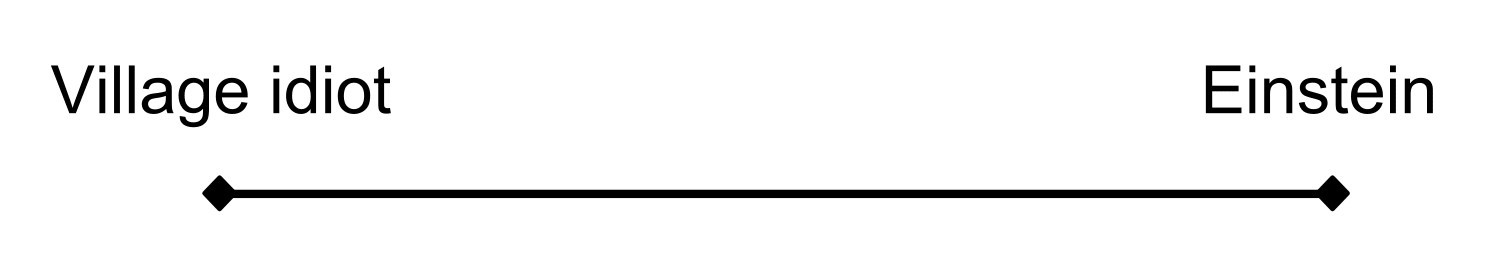
\includegraphics[scale=0.25]{Rationality20From20AI20to20Zombies2020Eliezer20Yudkowsky-img330.jpg}
 
\par}


\bigskip

{
\ \ \ ~}

{
\ \ \ But this is a rather \textit{parochial} view of intelligence.
Sure, in everyday life, we only deal socially with other humans---only
other humans are partners in the great game---and so we only
\textit{meet the minds} of intelligences ranging from village idiot to
Einstein. But what we really need to talk about Artificial Intelligence
or theoretical optima of rationality is \textit{this} intelligence
scale:}

{
\ \ \ ~}

{\centering
\ \ \  
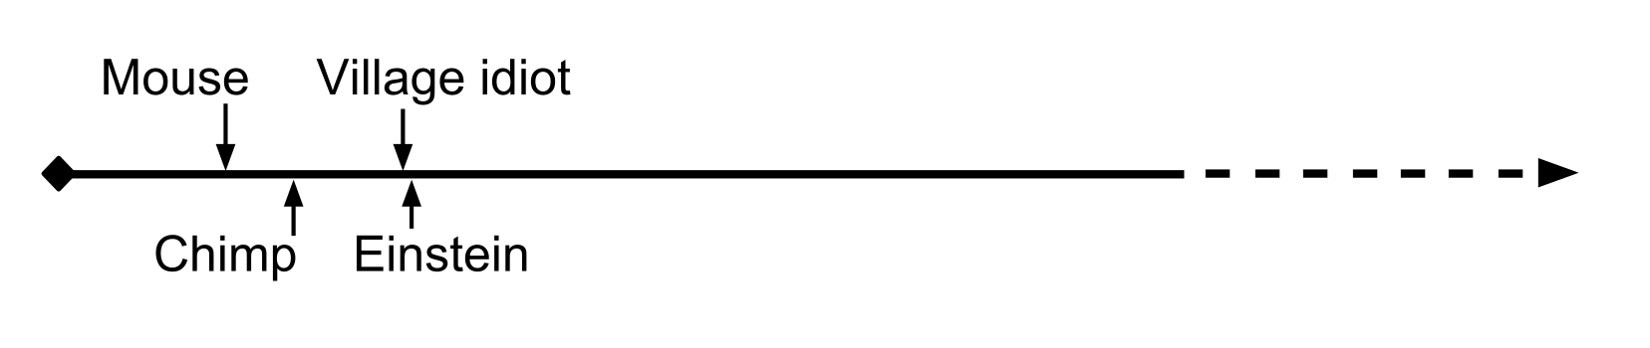
\includegraphics[scale=0.25]{Rationality20From20AI20to20Zombies2020Eliezer20Yudkowsky-img331.jpg}
 
\par}


\bigskip

{
\ \ \ ~}

{
\ \ \ For us humans, it seems that the scale of intelligence runs from
``village idiot'' at the bottom to
``Einstein'' at the top. Yet the
distance from ``village idiot'' to
``Einstein'' is tiny, in the space
of \textit{brain designs.} Einstein and the village idiot both have a
prefrontal cortex, a hippocampus, a cerebellum .~.~.}

{
\ \ \ Maybe Einstein has some minor genetic differences from the village
idiot, engine tweaks. But the brain-design-distance between Einstein
and the village idiot is nothing remotely like the
brain-design-distance between the village idiot and a chimpanzee. A
chimp couldn't tell the difference between Einstein and
the village idiot, and our descendants may not see much of a difference
either.}

{
\ \ \ Carl Shulman has observed that some academics who talk about
transhumanism seem to use the following scale of intelligence:}

{
\ \ \ ~}

{\centering
\ \ \  
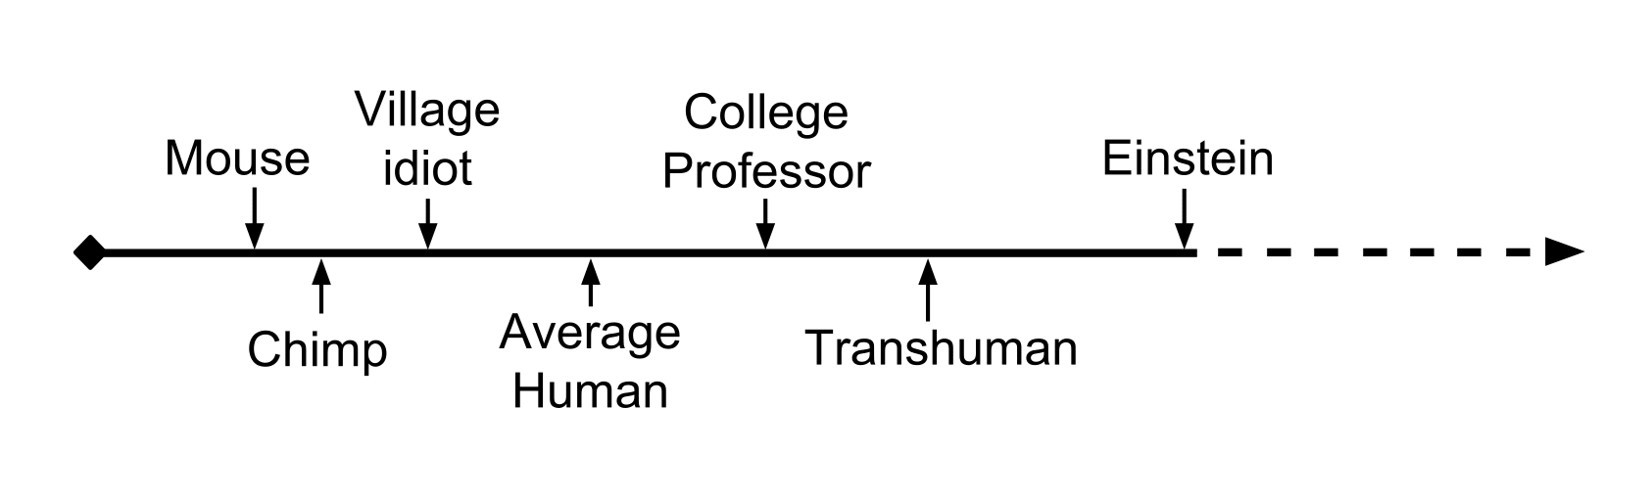
\includegraphics[scale=0.25]{Rationality20From20AI20to20Zombies2020Eliezer20Yudkowsky-img332.jpg}
 
\par}


\bigskip

{
\ \ \ ~}

{
\ \ \ Douglas Hofstadter actually said something like this, at the 2006
Singularity Summit. He looked at my diagram showing the
``village idiot'' next to
``Einstein,'' and said,
``That seems wrong to me; I think Einstein should be
way off on the right.''}

{
\ \ \ I was speechless. Especially because this was \textit{Douglas
Hofstadter}, one of my childhood heroes. It revealed a cultural gap
that I had never imagined existed.}

{
\ \ \ See, for me, what you would find toward the right side of the
scale was a Jupiter Brain. Einstein did not \textit{literally} have a
brain the size of a planet.}

{
\ \ \ On the right side of the scale, you would find Deep
Thought---Douglas Adams's original version, thank you,
not the chess player. The computer so intelligent that even before its
stupendous data banks were connected, when it was switched on for the
first time, it started from \textit{I think therefore I am} and got as
far as deducing the existence of rice pudding and income tax before
anyone managed to shut it off.}

{
\ \ \ Toward the right side of the scale, you would find the Elders of
Arisia, galactic overminds, Matrioshka brains, and the better class of
God. At the \textit{extreme} right end of the scale, Old One and the
Blight.}

{
\ \ \ Not frickin' Einstein.}

{
\ \ \ I'm sure Einstein was very smart for a human.
I'm sure a General Systems Vehicle would think that was
very cute of him.}

{
\ \ \ I call this a ``cultural gap''
because I was introduced to the concept of a Jupiter Brain at the age
of twelve.}

{
\ \ \ Now all of this, of course, is the logical fallacy of
generalization from fictional evidence.}

{
\ \ \ But it is an example of why---logical fallacy or not---I suspect
that reading science fiction does have a helpful effect on futurism.
Sometimes the alternative to a fictional acquaintance with worlds
outside your own is to have a mindset that is absolutely stuck in one
era: A world where humans exist, and have always existed, and always
will exist.}

{
\ \ \ The universe is 13.7 billion years old, people! \textit{Homo
sapiens sapiens} have only been around for a hundred thousand years or
thereabouts!}

{
\ \ \ Then again, I have met some people who never read science fiction,
but who do seem able to imagine outside their own world. And there are
science fiction fans who don't get it. I wish I knew
what ``it'' was, so I could bottle
it.}

{
\ \ \ In the previous essay, I wanted to talk about the
\textit{efficient use of evidence}, i.e., Einstein was cute for a human
but in an absolute sense he was around as efficient as the US
Department of Defense.}

{
\ \ \ So I had to talk about a civilization that included thousands of
Einsteins, thinking for decades. Because if I'd just
depicted a Bayesian superintelligence in a box, looking at a webcam,
people would think: ``But .~.~. how does it know how
to interpret a 2D picture?'' They
wouldn't put \textit{themselves} in the shoes of the
mere machine, even if it was called a ``Bayesian
superintelligence''; they wouldn't
apply even their \textit{own} creativity to the problem of what you
could extract from looking at a grid of bits.}

{
\ \ \ It would just be a ghost in a box, that happened to be called a
``Bayesian superintelligence.'' The
ghost hasn't been told anything about how to interpret
the input of a webcam; so, in their mental model, the ghost does not
know.}

{
\ \ \ As for whether it's realistic to suppose that one
Bayesian superintelligence can ``do all
that'' .~.~. i.e., the stuff that occurred to me on
first sitting down to the problem, writing out the story as I went
along .~.~.}

{
\ \ \ Well, let me put it this way: Remember how Jeffreyssai pointed out
that if the experience of having an important insight
doesn't take more than 5 minutes, this theoretically
gives you time for 5,760 insights per month? Assuming you sleep 8 hours
a day and have no important insights while sleeping, that is.}

{
\ \ \ Now humans cannot use themselves this efficiently. But humans are
not adapted for the task of scientific research. Humans are adapted to
chase deer across the savanna, throw spears into them, cook them, and
then---this is probably the part that takes most of the
brains---cleverly argue that they deserve to receive a larger share of
the meat.}

{
\ \ \ It's amazing that Albert Einstein managed to
repurpose a brain like that for the task of doing physics. This
deserves applause. It deserves more than applause, it deserves a place
in the Guinness Book of Records. Like successfully building the fastest
car ever to be made entirely out of Jello.}

{
\ \ \ How poorly did the blind idiot god (evolution) \textit{really}
design the human brain?}

{
\ \ \ This is something that can only be grasped through much study of
cognitive science, until the full horror begins to dawn upon you.}

{
\ \ \ All the biases we have discussed here should at least be a hint.}

{
\ \ \ Likewise the fact that the human brain must use its full power and
concentration, with trillions of synapses firing, to multiply out two
three-digit numbers without a paper and pencil.}

{
\ \ \ No more than Einstein made efficient use of his sensory data, did
his brain make efficient use of his neurons' firing.}

{
\ \ \ Of course, I have certain ulterior motives in saying all this. But
let it also be understood that, years ago, when I set out to be a
rationalist, the impossible unattainable ideal of intelligence that
inspired me was never Einstein.}

{
\ \ \ Carl Schurz said:}

{
\ \ \ Ideals are like stars. You will not succeed in touching them with
your hands. But, like the seafaring man on the desert of waters, you
choose them as your guides and following them you will reach your
destiny.}

{
\ \ \ So now you've caught a glimpse of one of my great
childhood role models---my dream of an AI. Only the dream, of course,
the reality not being available. I reached up to that dream, once upon
a time.}

{
\ \ \ And this helped me to some degree, and harmed me to some degree.}

{
\ \ \ For some ideals are like dreams: they come from within us, not
from outside. Mentor of Arisia proceeded from E. E.
``doc'' Smith's
imagination, not from any real thing. If you imagine what a Bayesian
superintelligence would say, it is only your own mind talking. Not like
a star, that you can follow from outside. You have to guess where your
ideals are, and if you guess wrong, you go astray.}

{
\ \ \ But do not limit your ideals to mere stars, to mere humans who
actually existed, especially if they were born more than fifty years
before you and are dead. Each succeeding generation has a chance to do
better. To let your ideals be composed only of humans, especially dead
ones, is to limit yourself to what has already been accomplished. You
will ask yourself, ``Do I dare to do this thing, which
Einstein could not do? Is this not \textit{lèse
majesté}?'' Well, if Einstein had sat around asking
himself, ``Am I allowed to do better than
Newton?'' he would not have gotten where he did. This
is the problem with following stars; at best, it gets you to the star.}

{
\ \ \ Your era supports you more than you realize, in unconscious
assumptions, in subtly improved technology of mind. Einstein was a nice
fellow, but he talked a deal of nonsense about an impersonal God, which
shows you how well he understood the art of careful thinking at a
higher level of abstraction than his own field. It may seem less like
sacrilege to think that if you have at least one imaginary galactic
supermind to compare with Einstein, so that he is not the far right end
of your intelligence scale.}

{
\ \ \ If you only try to do what seems humanly possible, you will ask
too little of yourself. When you imagine reaching up to some higher and
inconvenient goal, all the convenient reasons why it is
``not possible'' leap readily to
mind.}

{
\ \ \ The most important role models are dreams: they come from within
ourselves. To dream of anything less than what you conceive to be
perfection is to draw on less than the full power of the part of
yourself that dreams.}

{\centering
\ \ \ \ ~
\par}

{\centering
\ \ \ *
\par}

\mysection{Einstein's Superpowers}

{
\ \ \ There is a widespread tendency to talk (and think) as if Einstein,
Newton, and similar historical figures had superpowers---something
magical, something sacred, something beyond the mundane. (Remember,
there are many more ways to worship a thing than lighting candles
around its altar.) }

{
\ \ \ Once I unthinkingly thought this way too, with respect to Einstein
in particular, until reading Julian Barbour's
\textit{The End of Time} cured me of it.\textsuperscript{1}}

{
\ \ \ Barbour laid out the history of anti-epiphenomenal physics and
Mach's Principle; he described the historical
controversies that predated Mach---all this that stood behind Einstein
and was known to Einstein, when Einstein tackled his problem .~.~.}

{
\ \ \ And maybe I'm just imagining things---reading too
much of \textit{myself} into Barbour's book---but I
thought I heard Barbour very quietly shouting, coded between the polite
lines:}

{
\ \ \ What Einstein did \textit{isn't magic}, people! If
you all just \textit{looked at how he actually did it}, instead of
falling to your knees and worshiping him, maybe then
you'd be able to do it too!}

{
\ \ \ \textit{(Barbour did not actually say this. It does not appear in
the book text. It is not a Julian Barbour quote and should not be
attributed to him. Thank you.)}}

{
\ \ \ Maybe I'm mistaken, or extrapolating too far .~.~.
but I kinda suspect that Barbour once tried to explain to people how
you move further along Einstein's direction to get
timeless physics; and they sniffed scornfully and said,
``Oh, you think \textit{you're}
Einstein, do you?''}

{
\ \ \ John Baez's Crackpot Index, item 18:}

{
\ \ \ 10 points for each favorable comparison of yourself to Einstein,
or claim that special or general relativity are fundamentally misguided
(without good evidence).}

{
\ \ \ Item 30:}

{
\ \ \ 30 points for suggesting that Einstein, in his later years, was
groping his way towards the ideas you now advocate.}

{
\ \ \ Barbour never bothers to compare himself to Einstein, of course;
nor does he ever appeal to Einstein in support of timeless physics. I
mention these items on the Crackpot Index by way of showing how many
people compare themselves to Einstein, and what society generally
thinks of them.}

{
\ \ \ The crackpot sees Einstein as something magical, so they compare
themselves to Einstein by way of praising themselves as magical; they
think Einstein had superpowers and they think they have superpowers,
hence the comparison.}

{
\ \ \ But it is just the other side of the same coin, to think that
Einstein is sacred, and the crackpot is \textit{not} sacred, therefore
they have committed blasphemy in comparing themselves to Einstein.}

{
\ \ \ Suppose a bright young physicist says, ``I admire
Einstein's work, but personally, I hope to do
better.'' If someone is shocked and says,
``What! You haven't accomplished
anything remotely like what Einstein did; what makes you think
you're smarter than him?'' then they
are the other side of the crackpot's coin.}

{
\ \ \ The underlying problem is conflating social status and research
potential.}

{
\ \ \ Einstein has extremely high social status: because of his record
of accomplishments; because of \textit{how} he did it; and because
he's the physicist whose name even the general public
remembers, who brought honor to science itself.}

{
\ \ \ And we tend to mix up fame with other quantities, and we tend to
attribute people's behavior to dispositions rather than
situations.}

{
\ \ \ So there's this tendency to think that Einstein,
even before he was famous, already had an inherent disposition to be
Einstein---a potential \textit{as rare as his fame} and \textit{as
magical as his deeds.} So that if you claim to have the
\textit{potential} to do what Einstein did, \textit{it is just the same
as claiming Einstein's rank,} rising far above your
assigned status in the tribe.}

{
\ \ \ I'm not phrasing this well, but then,
I'm trying to dissect a confused thought: Einstein
belongs to a separate magisterium, the sacred magisterium. The sacred
magisterium is distinct from the mundane magisterium; you
can't set out to be Einstein in the way you can set out
to be a full professor or a CEO. Only beings with divine potential can
enter the sacred magisterium---and then it is only fulfilling a destiny
they already have. So if you say you want to outdo Einstein,
you're claiming to \textit{already be} part of the
sacred magisterium---you claim to have the same aura of destiny that
Einstein was born with, like a royal birthright .~.~.}

{
\ \ \ ``But Eliezer,'' you say,
``surely not \textit{everyone} can become
Einstein.''}

{
\ \ \ You mean to say, not everyone can \textit{do better} than
Einstein.}

{
\ \ \ ``Um .~.~. yeah, that's what I
meant.''}

{
\ \ \ Well .~.~. in the modern world, you may be correct. You probably
\textit{should} remember that I am a transhumanist, going around
looking at people thinking, ``You know, it just sucks
that not everyone has the potential to do better than Einstein, and
this seems like a fixable problem.'' It colors
one's attitude.}

{
\ \ \ But in the modern world, yes, not everyone has the potential to be
Einstein.}

{
\ \ \ Still .~.~. how can I put this .~.~.}

{
\ \ \ There's a phrase I once heard,
can't remember where: ``Just another
Jewish genius.'' Some poet or author or philosopher
or other, brilliant at a young age, doing something not tremendously
important in the grand scheme of things, not all that influential, who
ended up being dismissed as ``Just another Jewish
genius.''}

{
\ \ \ If Einstein had chosen the wrong angle of attack on his
problem---if he hadn't chosen a sufficiently important
problem to work on---if he hadn't persisted for
years---if he'd taken any number of wrong turns---or if
someone else had solved the problem first---then dear Albert would have
ended up as just another Jewish genius.}

{
\ \ \ Geniuses are rare, but not all \textit{that} rare. It is not all
that implausible to lay claim to the kind of intellect that can get you
dismissed as ``just another Jewish
genius'' or ``just another brilliant
mind who never did anything interesting with their
life.'' The associated social status here is not high
enough to be sacred, so it should seem like an ordinarily evaluable
claim.}

{
\ \ \ But what separates people like this from becoming Einstein, I
suspect, is no innate defect of brilliance. It's things
like ``lack of an interesting
problem''---or, to put the blame where it belongs,
``failing to choose an important
problem.'' It is very easy to fail at this because of
the cached thought problem: Tell people to choose an important problem
and they will choose the first cache hit for
``important problem'' that pops into
their heads, like ``global warming''
or ``string theory.''}

{
\ \ \ The truly important problems are often the ones
you're not even considering, because they appear to be
impossible, or, um, \textit{actually difficult}, or worst of all,
\textit{not clear how to solve}. If you worked on them for years, they
might not seem so impossible .~.~. but this is an extra and unusual
insight; naive realism will tell you that solvable problems look
solvable, and impossible-looking problems are impossible.}

{
\ \ \ Then you have to come up with a new and \textit{worthwhile} angle
of attack. Most people who are not allergic to novelty will go too far
in the other direction, and fall into an affective death spiral.}

{
\ \ \ And then you've got to bang your head on the
problem for years, without being distracted by the temptations of
easier living. ``Life is what happens while we are
making other plans,'' as the saying goes, and if you
want to fulfill your other plans, you've often got to
be ready to turn down life.}

{
\ \ \ Society is not set up to support you while you work, either.}

{
\ \ \ The point being, the problem is not that you need an aura of
destiny and the aura of destiny is missing. If you'd
met Albert before he published his papers, you would have perceived no
aura of destiny about him to match his future high status. He would
seem like just another Jewish genius.}

{
\ \ \ This is not because the royal birthright is \textit{concealed},
but because it simply is \textit{not there.} It is \textit{not
necessary.} There \textit{is no} separate magisterium for people who do
important things.}

{
\ \ \ I say this, because I want to do important things with my life,
and I have a genuinely important problem, and an angle of attack, and
I've been banging my head on it for years, and
I've managed to set up a support structure for it; and
I very frequently meet people who, in one way or another, say:
``Yeah? Let's see your aura of
destiny, buddy.''}

{
\ \ \ What impressed me about Julian Barbour was a quality that I
don't think anyone would have known how to fake without
actually \textit{having} it: Barbour seemed to have \textit{seen
through} Einstein---he talked about Einstein as if everything Einstein
had done was perfectly understandable and mundane.}

{
\ \ \ Though even having realized this, to me it still came as a shock,
when Barbour said something along the lines of, ``Now
here's where Einstein failed to apply his own methods,
and missed the key insight---'' But the shock was
fleeting, I knew the Law: \textit{No gods, no magic, and ancient heroes
are milestones to tick off in your rearview mirror.}}

{
\ \ \ This \textit{seeing through} is something one has to
\textit{achieve}, an insight one has to discover. You cannot see
through Einstein just by saying, ``Einstein is
mundane!'' if his work still seems like magic unto
you. That would be like declaring ``Consciousness must
reduce to neurons!'' without having any idea of how
to do it. It's true, but it doesn't
solve the problem.}

{
\ \ \ I'm not going to tell you that Einstein was an
ordinary bloke oversold by the media, or that deep down he was a
regular schmuck just like everyone else. That would be going
\textit{much} too far. To walk this path, one must acquire abilities
some consider to be .~.~. unnatural. I take a special joy in doing
things that people call ``humanly
impossible,'' because it shows that
I'm growing up.}

{
\ \ \ Yet the way that you acquire magical powers is not by being born
with them, but by seeing, with a sudden shock, that they \textit{really
are} perfectly normal.}

{
\ \ \ This is a general principle in life.}

{\centering
\ \ \ \ ~
\par}

{\centering
\ \ \ *
\par}


\bigskip

{
\ \ \ 1. Julian Barbour, \textit{The End of Time: The Next Revolution in
Physics}, 1st ed. (New York: Oxford University Press, 1999).}

\mysection{Class Project}

{
\ \ \ ``Do as well as Einstein?''
Jeffreyssai said, incredulously. ``\textit{Just} as
well as Einstein? Albert Einstein was a great scientist of his era, but
that was his era, not this one! Einstein did not comprehend the
Bayesian methods; he lived before the cognitive biases were discovered;
he had no scientific grasp of his own thought processes. He was too
caught up in the drama of rejecting his era's quantum
mechanics to actually \textit{fix} it. And while I grant that Einstein
reasoned cleanly in the matter of General Relativity---barring that
matter of the cosmological constant---he took ten years to do it. Too
slow!'' }

{
\ \ \ ``\textit{Too slow?}'' repeated
Taji incredulously.}

{
\ \ \ ``Too slow! If Einstein were in this classroom
now, rather than Earth of the negative first century, I would rap his
knuckles! \textit{You will not try to do as well as Einstein! You will
aspire to do BETTER than Einstein or you may as well not
bother!}''}

{
\ \ \ Jeffreyssai shook his head. ``Well,
I've given you enough hints. It is time to test your
skills. Now, I know that the other \textit{beisutsukai}
don't think much of my class projects
.~.~.'' Jeffreyssai paused significantly.}

{
\ \ \ Brennan inwardly sighed. He'd heard this line many
times before, in the Bardic Conspiracy, the Competitive Conspiracy:
\textit{The other teachers think my assignments are too easy, you
should be grateful,} followed by some ridiculously difficult task---}

{
\ \ \ ``They say,'' Jeffreyssai said,
``that my projects are too hard; insanely hard; that
they pass from the realm of madness into the realm of Sparta; that
Laplace himself would catch on fire; they accuse me of trying to tear
apart my students' souls---''}

{
\ \ \ \textit{Oh, crap.}}

{
\ \ \ ``But there is a reason,''
Jeffreyssai said, ``why many of my students have
achieved great things; and by that I do not mean high rank in the
Bayesian Conspiracy. I expected much of them, and they came to expect
much of themselves. So .~.~.''}

{
\ \ \ Jeffreyssai took a moment to look over his increasingly disturbed
students. ``Here is your assignment. Of quantum
mechanics, and General Relativity, you have been told. This is the
limit of Eld science, and hence, the limit of public knowledge. The
five of you, working on your own, are to produce the correct theory of
quantum gravity. Your time limit is one month.''}

{
\ \ \ ``\textit{What?}'' said
Brennan, Taji, Styrlyn, and Yin. Hiriwa gave them a puzzled look.}

{
\ \ \ ``Should you succeed,''
Jeffreyssai continued, ``you will be promoted to
\textit{beisutsukai} of the second \textit{dan} and sixth level. We
will see if you have learned speed. Your clock
starts---\textit{now}.''}

{
\ \ \ And Jeffreyssai strode out of the room, slamming the door behind
him.}

{
\ \ \ ``This is crazy!'' Taji cried.}

{
\ \ \ Hiriwa looked at Taji, bemused. ``The solution is
not known to us. How can you know it is so
difficult?''}

{
\ \ \ ``Because we \textit{knew} about this problem
back in the Eld days! Eld scientists worked on this problem for a lot
longer than one month.''}

{
\ \ \ Hiriwa shrugged. ``They were still arguing about
many-worlds too, weren't they?''}

{
\ \ \ ``\textit{Enough! There's no
time!}''}

{
\ \ \ The other four students looked to Styrlyn, remembering that he was
said to rank high in the Cooperative Conspiracy. There was a brief
moment of weighing, of assessing, and then Styrlyn was their leader.}

{
\ \ \ Styrlyn took a great breath. ``We need a list of
approaches. Write down all the angles you can think of.
Independently---we need your individual components before we start
combining. In five minutes, I'll ask each of you for
your best idea first. \textit{No wasted thoughts!
Go!}''}

{
\ \ \ Brennan grabbed a sheet and his tracer, set the tip to the
surface, and then paused. He couldn't think of anything
clever to say about unifying General Relativity and quantum mechanics
.~.~.}

{
\ \ \ The other students were already writing.}

{
\ \ \ Brennan tapped the tip, once, twice, thrice. General Relativity
and quantum mechanics .~.~.}

{
\ \ \ Taji put his first sheet aside, grabbed another.}

{
\ \ \ Finally, Brennan, for lack of anything clever to say, wrote down
the obvious.}

{
\ \ \ Minutes later, when Styrlyn called time, it was still all he had
written.}

{
\ \ \ ``All right,'' Styrlyn said,
``your best idea. Or the idea you most want the rest
of us to take into account in our second components. Taji,
go!''}

{
\ \ \ Taji looked over his sheets. ``Okay, I think
we've got to assume that every avenue that Eld science
was trying is a blind alley, or they would have found it. And if this
is possible to do in one month, the answer must be, in some sense,
elegant. So no multiple dimensions. If we start doing anything that
looks like we should call it `string
theory,' we'd better stop. Maybe begin
by considering how failure to understand decoherence could have led Eld
science astray in quantizing gravity.''}

{
\ \ \ ``The opposite of folly is
folly,'' Hiriwa said. ``Let us
pretend that Eld science never existed.''}

{
\ \ \ ``No criticisms yet!'' said
Styrlyn. ``Hiriwa, your
suggestion?''}

{
\ \ \ ``Get rid of the infinities,''
said Hiriwa, ``extirpate that which permits them. It
should not be a matter of cleverness with integrals. A
\textit{representation} that allows infinity must be
false-to-fact.''}

{
\ \ \ ``Yin.''}

{
\ \ \ ``We know from common sense,''
Yin said, ``that if we stepped outside the universe,
we would see time laid out all at once, reality like a crystal. But I
once encountered a hint that physics is timeless in a deeper sense than
that.'' Yin's eyes were distant,
remembering. ``Years ago, I found an abandoned city;
it had been uninhabited for eras, I think. And behind a door whose
locks were broken, carved into one wall: quote \textit{.ua sai .ei mi
vimcu ty bu le mekso} unquote.''}

{
\ \ \ Brennan translated: \textit{Eureka! Eliminate t from the
equations.} And written in Lojban, the sacred language of science,
which meant the unknown writer had thought it to be true.}

{
\ \ \ ``The `timeless
physics' of which we've all heard
rumors,'' Yin said, ``may be
timeless in a very literal sense.''}

{
\ \ \ ``My own contribution,''
Styrlyn said. ``The quantum physics
we've learned is over joint positional configurations.
It seems like we should be able to take that apart into a spatially
local representation, in terms of invariant distant entanglements.
Finding that representation might help us integrate with General
Relativity, whose curvature is local.''}

{
\ \ \ ``A strangely \textit{individualist}
perspective,'' Taji murmured, ``for
one of the Cooperative Conspiracy.''}

{
\ \ \ Styrlyn shook his head. ``You misunderstand us,
then. The first lesson we learn is that groups are made of people .~.~.
no, there is no time for politics. Brennan!''}

{
\ \ \ Brennan shrugged. ``Not much, I'm
afraid, only the obvious. Inertial mass-energy was always observed to
equal gravitational mass-energy, and Einstein showed that they were
necessarily the same. So why is the
`energy' that is an eigenvalue of the
quantum Hamiltonian \textit{necessarily} the same as the
`energy' quantity that appears in the
equations of General Relativity? Why should spacetime curve at the same
rate that the little arrows rotate?''}

{
\ \ \ There was a brief pause.}

{
\ \ \ Yin frowned. ``That seems \textit{too} obvious.
Wouldn't Eld science have figured it out
already?''}

{
\ \ \ ``Forget Eld science existed,''
Hiriwa said. ``The question stands: we need the
answer, whether it was known in ancient times or not. It cannot
possibly be \textit{coincidence.}''}

{
\ \ \ Taji's eyes were abstracted.
``Perhaps it would be possible to show that an
exception to the equality would violate some conservation law
.~.~.''}

{
\ \ \ ``That is not where Brennan
pointed,'' Hiriwa interrupted. ``He
did not ask for a proof that they must be set equal, given some
appealing principle; he asked for a view in which the two are one and
cannot be divided even conceptually, as was accomplished for inertial
mass-energy and gravitational mass-energy. For we must assume that the
beauty of the whole arises from the fundamental laws, and not the other
way around. Fair-rephrasing?''}

{
\ \ \ ``Fair-rephrasing,'' Brennan
replied.}

{
\ \ \ Silence reigned for thirty-seven seconds, as the five pondered the
five suggestions.}

{
\ \ \ ``I have an idea .~.~.''}

{\centering
\ \ \ \ ~
\par}

{\centering
\ \ \ *
\par}

\mysectionnn{Interlude A Technical Explanation of Technical Explanation}

{
\ \ \ As Jaynes emphasizes, the theorems of Bayesian probability theory
are just that---\textit{mathematical theorems} that follow inevitably
from Bayesian axioms.\textsuperscript{1} One might naively think that
there would be no controversy about mathematical theorems. But when do
the theorems apply? How do we use the theorems in real-world problems?
The Intuitive Explanation tries to avoid controversy, but the Technical
Explanation willfully walks into the whirling helicopter blades.
Bluntly, the reasoning in the Technical Explanation does not represent
the unanimous consensus of Earth's entire planetary
community of Bayesian researchers. At least, not yet.}

{
\ \ \ Where the Intuitive Explanation focused on providing a firm grasp
of Bayesian basics, A Technical Explanation of Technical Explanation
builds, on a Bayesian foundation, theses about human rationality and
philosophy of science. The Technical Explanation of Technical
Explanation is so named because it begins with this question:}

{
\ \ \ ``What is the difference between a technical
understanding and a verbal understanding?''}

{
\ \ \ As a child I read books of popular physics, and fancied myself
knowledgeable; I thought I knew that sound was waves of air, that light
was waves of electromagnetism, that matter was waves of complex
probability amplitudes. When I grew up, I read the \textit{Feynman
Lectures on Physics} and took the time to understand
``the wave
equation.''\textsuperscript{2} And then I realized
that up to that point, I had not understood or believed
``sound is waves'' in anything like
the way a physicist means and believes that sentence.}

{
\ \ \ So that is the difference between a technical understanding and a
verbal understanding.}

{
\ \ \ Do you believe that? If so, you should have applied the knowledge,
and said: ``But why didn't you give a
technical explanation instead of a verbal
explanation?''}

{
\ \ \ Visualize \textit{probability density} or \textit{probability
mass}{}---probability as a lump of clay that you must distribute over
possible outcomes.}

{
\ \ \ Let's say there's a little light
that can flash \textit{red}, \textit{blue}, or \textit{green} each time
you press a button. The light flashes one and only one color on each
press of the button; the possibilities are mutually exclusive.
You're trying to predict the color of the next flash.
On each try, you have a weight of clay, the probability mass, that you
have to distribute over the possibilities red, green, and blue. You
might put a fourth of your clay on the green possibility, a fourth of
your clay on the blue possibility, and half your clay on the red
possibility---like assigning probabilities of 25\% to green, 25\% to
blue, and 50\% to red. The metaphor is that \textit{probability is a
conserved resource}, to dole out sparingly. If you think that blue is
more likely to flash on the next experiment, you can assign a higher
probability to blue, but you have to take the probability mass from the
other hypotheses---maybe steal some clay from red and add it to blue.
You can never get any more clay. Your probabilities
can't sum to more than 1.0 (100\%). You
can't predict a 75\% chance of seeing red and an 80\%
chance of seeing blue.}

{
\ \ \ Why would you want to be careful with your probability mass, or
dole it out sparingly? Why not slop probability all over the place?
Let's shift the metaphor from clay to money. You can
bet up to a dollar of play money on each press of the button. An
experimenter stands nearby, and pays you an amount of real money that
depends on how much play money you bet on the \textit{winning} light.
We don't care how you distributed your remaining play
money over the losing lights. The only thing that matters is how much
you bet on the light that actually won.}

{
\ \ \ But we must carefully construct the scoring rule used to pay off
the winners, if we want the players to be careful with their bets.
Suppose the experimenter pays each player real money equal to the play
money bet on the winning color. Under this scoring rule, if you observe
that red comes up six times out of ten, your best strategy is to bet,
not 60 cents on red, but the entire dollar on red, and you
don't care about the frequencies of blue and green.
Why? Let's say that blue and green each come up around
two times out of ten. And suppose you bet 60 cents on red, 20 cents on
blue, and 20 cents on green. In this case, six times out of ten you
would win 60 cents, and four times out of ten you would win 20 cents,
for an average payoff of 44 cents. Under that scoring rule, it makes
more sense to allocate the entire dollar to red, and win an entire
dollar six times out of ten. Four times out of ten you would win
nothing. Your average payoff would be 60 cents.}

{
\ \ \ If we wrote down the function for the payoff, it would be Payoff =
P(winner), where P(winner) is the amount of play money you bet on the
winning color on that round. If we wrote down the function for the
expected payoff given that Payoff rule, it would be:}

%putting \mathrm{Payoff} in causes lualatex to run out of memory
\begin{equation*}
  \mathrm{Expectation}(\mathrm{Payof}\mathrm{f}) = \sum_{colors} P(\mathrm{color})\times F(\mathrm{color}).
\end{equation*}
%\begin{equation*}
%  \mathrm{Expectation}(\mathrm{Payoff} = \sum_{colors} P(\mathrm{color})\times F(\mathrm{color}) .
%\end{equation*}



\bigskip

{
\ \ \ P(color) is the amount of play money you bet on a color, and
F(color) is the frequency with which that color wins.}

{
\ \ \ Suppose that the actual frequencies of the lights are 30\% blue,
20\% green, and 50\% red. And suppose that on each round I bet 40\% on
blue, 50\% on green, and 10\% on red. I would get 40 cents 30\% of the
time, 50 cents 20\% of the time, and 10 cents 50\% of the time, for an
average payoff of \$0.12 + \$0.10 + \$0.05 or \$0.27. That is:}

{\centering
\ \ \ P(color) = play money assigned to that color
\par}


\bigskip

{\centering
\ \ \ F(color) = frequency with which that color wins
\par}


\bigskip

{\centering
\ \ \ Payoff = P(winner) = amount of play money allocated to winning
color.
\par}


\bigskip

{
\ \ \ Actual frequencies of winning:}

{\centering
\ \ \ F(blue) = 30\%
\par}


\bigskip

{\centering
\ \ \ F(green) = 20\%
\par}


\bigskip

{\centering
\ \ \ F(red) = 50\%.
\par}


\bigskip

{
\ \ \ In the long run, red wins 50\% of the time, green wins 20\% of the
time, and blue wins 30\% of the time. So our \textit{average} payoff on
each round is 50\% of the payoff if red wins, plus 20\% of the payoff
if green wins, plus 30\% of the payoff if blue wins.}

{
\ \ \ The payoff is a function of the winning color and the betting
scheme. We want to compute the \textit{average} payoff, given a betting
scheme and the \textit{frequencies} at which each color wins. The
mathematical term for this kind of computation, taking a function of
each case and weighting it by the frequency of that case, is an
\textit{expectation}. Thus, to compute our \textit{expected payoff} we
would calculate:}


\begin{equation*}
  \mathrm{Expectation}(\mathrm{Payof}\mathrm{f}) = \sum_{colors} P(\mathrm{color}) F(\mathrm{color})
\end{equation*}
%\begin{equation*}
%  \mathrm{Expectation}(\mathrm{Payoff} = \sum_{colors} P(\mathrm{color}) F(\mathrm{color})
%\end{equation*}


\bigskip

{\centering
\ \ \ = P(blue) {\texttimes} F(blue) + P(green) {\texttimes} F(green) +
P(red) {\texttimes} F(red)
\par}


\bigskip

{\centering
\ \ \ = \$0.40 {\texttimes} 30\% + \$0.50 {\texttimes} 20\% + \$0.10
{\texttimes} 50\%
\par}


\bigskip

{\centering
\ \ \ = \$0.12 + \$0.10 + \$0.05
\par}


\bigskip

{\centering
\ \ \ = \$0.27.
\par}


\bigskip

{
\ \ \ With this betting scheme I'll win, on average,
around 27 cents per round.}

{
\ \ \ I allocated my play money in a grossly arbitrary way, and the
question arises: Can I increase my expected payoff by allocating my
play money more wisely? \textit{Given the scoring rule provided}, I
maximize my expected payoff by allocating my \textit{entire} dollar to
red. Despite my \textit{expected} payoff of 50 cents per round, the
light might \textit{actually} flash green, blue, blue, green, green and
I would receive an \textit{actual} payoff of zero. However, the chance
of the light's coming up non-red on five successive
rounds is approximately 3\%. Compare the red/blue card game in Lawful
Uncertainty.}

{
\ \ \ A \textit{proper scoring rule} is a rule for scoring bets so that
you maximize your expected payoff by betting play money that exactly
equals the chance of that color flashing. We want a scoring rule so
that if the lights actually flash at the frequencies 30\% blue, 20\%
green, and 50\% red, you can maximize your average payoff \textit{only}
by betting 30 cents on blue, 20 cents on green, and 50 cents on red. A
proper scoring rule is one that forces your optimal bet to exactly
report your estimate of the probabilities. (This is also sometimes
known as a \textit{strictly proper scoring rule}.) As
we've seen, not all scoring rules have this property;
and if you invent a plausible-sounding scoring rule at random, it
probably \textit{won't} have the property.}

{
\ \ \ One rule with this proper property is to pay a dollar minus the
squared error of the bet, rather than the bet itself---if you bet 30
cents on the winning light, your error would be 70 cents, your squared
error would be 49 cents (0.7\textsuperscript{2} = 0.49), and a dollar
minus your squared error would be 51 cents.\textsuperscript{3}
(Presumably your play money is denominated in the square root of cents,
so that the squared error is a monetary sum.)}

{
\ \ \ We shall \textit{not} use the squared-error rule. Ordinary
statisticians take the squared error of everything in sight, but not
Bayesian statisticians.}

{
\ \ \ We add a new requirement: we require, not only a proper scoring
rule, but that our proper scoring rule gives us the same answer whether
we apply it to rounds individually or combined. This is what Bayesians
do instead of taking the squared error of things; we require
invariances.}

{
\ \ \ Suppose I press the button twice in a row. There are nine possible
outcomes: green-green, green-blue, green-red, blue-green, blue-blue,
blue-red, red-green, red-blue, and red-red. Suppose that green wins,
and then blue wins. The experimenter would assign the first score based
on our probability assignments for P(green\textsubscript{1}) and the
second score based on
P(blue\textsubscript{2}{\textbar}green\textsubscript{1}).\textsuperscript{4}
We would make two predictions, and get two scores. Our first prediction
was the probability we assigned to the color that won on the first
round, green. Our second prediction was our probability that blue would
win on the second round, \textit{given} that green won on the first
round. Why do we need to write
P(blue\textsubscript{2}{\textbar}green\textsubscript{1}) instead of
just P(blue\textsubscript{2})? Because you might have a hypothesis
about the flashing light that says ``blue never
follows green,'' or ``blue always
follows green'' or ``blue follows
green with 70\% probability.'' If this is so, then
after seeing green on the first round, you might want to revise your
prediction---change your bets---for the second round. You can always
revise your predictions right up to the moment the experimenter presses
the button, using every scrap of information; but after the light
flashes it is too late to change your bet.}

{
\ \ \ Suppose the actual outcome is green\textsubscript{1} followed by
blue\textsubscript{2}. We require this invariance: I must get the same
total score, regardless of whether:}

{
\ \ \ I am scored twice, first on my prediction for
P(green\textsubscript{1}), and second on my prediction for
P(blue\textsubscript{2}{\textbar}green\textsubscript{1}).}

{
\ \ \ I am scored once for my joint prediction P(green\textsubscript{1}
and blue\textsubscript{2}).}

{
\ \ \ Suppose I assign a 60\% probability to green\textsubscript{1}, and
then the green light flashes. I must now produce probabilities for the
colors on the second round. I assess the possibility
blue\textsubscript{2}, and allocate it 25\% of my probability mass. Lo
and behold, on the second round the light flashes blue. So on the first
round my bet on the winning color was 60\%, and on the second round my
bet on the winning color was 25\%. But I might also, at the start of
the experiment and after assigning P(green\textsubscript{1}), imagine
that the light first flashes green, imagine updating my theories based
on that information, and then say what confidence I will give to blue
on the next round if the first round is green. That is, I generate the
probabilities P(green\textsubscript{1}) and
P(blue\textsubscript{2}{\textbar}green\textsubscript{1}). By
multiplying these two probabilities together we would get the joint
probability, P(green\textsubscript{1} and blue\textsubscript{2}) =
15\%.}

{
\ \ \ A double experiment has nine possible outcomes. If I generate nine
probabilities for P(green\textsubscript{1}, green\textsubscript{2}),
P(green\textsubscript{1}, blue\textsubscript{2}), .~.~.~,
P(red\textsubscript{1}, blue\textsubscript{2}), P(red\textsubscript{1},
red\textsubscript{2}), the probability mass must sum to no more than
one. I am giving predictions for nine mutually exclusive possibilities
of a ``double experiment.''}

{
\ \ \ We require a scoring rule (and maybe it won't look
like anything an ordinary bookie would ever use) such that my score
doesn't change regardless of whether we consider the
double result as two predictions or one prediction. I can treat the
sequence of two results as a single experiment,
``press the button twice,'' and be
scored on my prediction for P(blue\textsubscript{2},
green\textsubscript{1}) = 15\%. Or I can be scored once for my first
prediction P(green\textsubscript{1}) = 60\%, then again on my
prediction P(blue\textsubscript{2}{\textbar}green\textsubscript{1}) =
25\%. We require the same \textit{total} score in either case, so that
it doesn't matter how we slice up the experiments and
the predictions---the \textit{total} score is always exactly the same.
This is our invariance.}

{
\ \ \ We have just required:}

{\centering
\ \ \ Score[P(green\textsubscript{1},blue\textsubscript{2})] =
Score[P(green\textsubscript{1})] +
Score[P(blue\textsubscript{2}{\textbar}green\textsubscript{1})].
\par}


\bigskip

{
\ \ \ And we already know:}

{\centering
\ \ \ P(green\textsubscript{1},blue\textsubscript{2}) =
P(green\textsubscript{1}) {\texttimes}
P(blue\textsubscript{2}{\textbar}green\textsubscript{1}).
\par}


\bigskip

{
\ \ \ The only possible scoring rule is:}

{\centering
\ \ \ Score(P) = log(P).
\par}


\bigskip

{
\ \ \ The new scoring rule is that your score is the \textit{logarithm}
of the probability you assigned to the winner.}

{
\ \ \ The base of the logarithm is arbitrary---whether we use the
logarithm base ten or the logarithm base two, the scoring rule has the
desired invariance. But we must choose some actual base. A
mathematician would choose base e; an engineer would choose base ten; a
computer scientist would choose base two. If we use base ten, we can
convert to \textit{decibels}, as in the Intuitive Explanation; but
sometimes bits are easier to manipulate.}

{
\ \ \ The logarithm scoring rule is proper---it has its expected maximum
when we say our exact anticipations; it rewards honesty. If we think
the blue light has a 60\% probability of flashing, and we calculate our
expected payoff for different betting schemas, we find that we maximize
our expected payoff by telling the experimenter
``60\%.'' (Readers with calculus can
verify this.) The scoring rule also gives an invariant total,
regardless of whether pressing the button twice counts as
``one experiment'' or
``two experiments.'' However,
payoffs are now all \textit{negative}, since we are taking the
logarithm of the probability and the probability is between zero and
one. The logarithm base ten of 0.1 is -1; the logarithm base ten of
0.01 is -2. That's okay. We accepted that the scoring
rule might not look like anything a real bookie would ever use. If you
like, you can imagine that the experimenter has a pile of money, and at
the end of the experiment they award you some amount minus your large
negative score. (Er, the amount plus your negative score.) Maybe the
experimenter has a hundred dollars, and at the end of a hundred rounds
you accumulated a score of -48, so you get \$52 dollars.}

{
\ \ \ A score of -48 in what base? We can eliminate the ambiguity in the
score by specifying units. Ten decibels equals a factor of 10; negative
ten decibels equals a factor of 1/10. Assigning a probability of 0.01
to the actual outcome would score -20 decibels. A probability of 0.03
would score -15 decibels. Sometimes we may use bits: 1 bit is a factor
of 2, -1 bit is a factor of 1/2. A probability of 0.25 would score -2
bits; a probability of 0.03 would score around -5 bits.}

{
\ \ \ If you arrive at a probability assessment P for each color, with
P(red), P(blue), P(green), then your \textit{expected score} is:}

{\centering
\ \ \ Score(P) = log(P)
\par}


\bigskip

\begin{equation*}
  \mathrm{Expectation}(\mathrm{Score}) = \sum_{colors}P(\mathrm{color})\times\log(P(\mathrm{color})).
\end{equation*}


\bigskip

{
\ \ \ Suppose you had probabilities of 25\% red, 50\% blue, and 25\%
green. Let's think in base 2 for a moment, to make
things simpler. Your expected score is:}

{\centering
\ \ \ Score(red) = $-$2 bits, flashes 25\% of the time,
\par}


\bigskip

{\centering
\ \ \ Score(blue) = $-$1 bit, flashes 50\% of the time,
\par}


\bigskip

{\centering
\ \ \ Score(green) = $-$2 bits, flashes 25\% of the time,
\par}


\bigskip

{\centering
\ \ \ Expectation(Score) = $-$1.5 bits.
\par}


\bigskip

{
\ \ \ Contrast our Bayesian scoring rule with the ordinary or colloquial
way of speaking about degrees of belief, where someone might casually
say, ``I'm 98\% certain that canola
oil contains more omega-3 fats than olive oil.'' What
they really mean by this is that they feel 98\%
certain---there's something like a little progress bar
that measures the strength of the emotion of certainty, and this
progress bar is 98\% full. And the emotional progress bar probably
wouldn't be exactly 98\% full, if we had some way to
measure. The word ``98\%'' is just a
colloquial way of saying: ``I'm almost
but not entirely certain.'' It
doesn't mean that you could get the highest expected
payoff by betting exactly 98 cents of play money on that outcome. You
should only assign a \textit{calibrated confidence} of 98\% if
you're confident enough that you think you could answer
a hundred similar questions, of equal difficulty, one after the other,
each independent from the others, and be wrong, on average, about
twice. We'll keep track of how often
you're right, over time, and if it turns out that when
you say ``90\% sure''
you're right about seven times out of ten, then
we'll say you're \textit{poorly
calibrated}.}

{
\ \ \ If you say ``98\% probable'' a
thousand times, and you are surprised only five times, we still ding
you for poor calibration. You're allocating too much
probability mass to the possibility that you're wrong.
You should say ``99.5\% probable''
to maximize your score. The scoring rule rewards \textit{accurate}
calibration, encouraging neither humility nor arrogance.}

{
\ \ \ At this point it may occur to some readers that
there's an obvious way to achieve perfect
calibration---just flip a coin for every yes-or-no question, and assign
your answer a confidence of 50\%. You say 50\% and
you're right half the time. Isn't that
perfect calibration? Yes. But calibration is only one component of our
Bayesian score; the other component is \textit{discrimination}.}

{
\ \ \ Suppose I ask you ten yes-or-no questions. You know absolutely
nothing about the subject, so on each question you divide your
probability mass fifty-fifty between
``Yes'' and
``No.'' Congratulations,
you're perfectly calibrated---answers for which you
said ``50\% probability'' were true
exactly half the time. This is true regardless of the sequence of
correct answers or how many answers were Yes. In ten experiments you
said ``50\%'' on twenty
occasions---you said ``50\%'' to
Yes\textsubscript{1}, No\textsubscript{1}, Yes\textsubscript{2},
No\textsubscript{2}, Yes\textsubscript{3}, No\textsubscript{3}, .~.~.
On ten of those occasions the answer was correct, the occasions:
Yes\textsubscript{1}, No\textsubscript{2}, No\textsubscript{3}, .~.~.
And on ten of those occasions the answer was incorrect:
No\textsubscript{1}, Yes\textsubscript{2}, Yes\textsubscript{3}, .~.~.}

{
\ \ \ Now I give my own answers, putting more effort into it, trying to
discriminate whether Yes or No is the correct answer. I assign 90\%
confidence to each of my favored answers, and my favored answer is
wrong twice. I'm more poorly calibrated than you. I
said ``90\%'' on ten occasions and I
was wrong two times. The next time someone listens to me, they may
mentally translate ``90\%'' into
80\%, knowing that when I'm 90\% sure,
I'm right about 80\% of the time. But the probability
you assigned to the final outcome is 1/2 to the tenth power, which is
0.001 or 1/1,024. The probability I assigned to the final outcome is
90\% to the eighth power times 10\% to the second power,
0.9\textsuperscript{8} {\texttimes} 0.1\textsuperscript{2}, which works
out to 0.004 or 0.4\%. Your calibration is perfect and mine
isn't, but my better \textit{discrimination} between
right and wrong answers more than makes up for it. My final score is
higher---I assigned a greater joint probability to the final outcome of
the entire experiment. If I'd been less overconfident
and better calibrated, the probability I assigned to the final outcome
would have been 0.8\textsuperscript{8} {\texttimes}
0.2\textsuperscript{2}, which works out to 0.006 or 6\%.}

{
\ \ \ Is it possible to do even better? Sure. You could have guessed
every single answer correctly, and assigned a probability of 99\% to
each of your answers. Then the probability you assigned to the entire
experimental outcome would be 0.99\textsuperscript{10} ${\approx}$
90\%.}

{
\ \ \ Your \textit{score} would be log (90\%), which is -0.45 decibels
or -0.15 bits. We need to take the logarithm so that if I try to
maximize my \textit{expected score}, ${\sum}$ P {\texttimes} log (P), I
have no motive to cheat. Without the logarithm rule, I would maximize
my expected score by assigning all my probability mass to the most
probable outcome. Also, without the logarithm rule, my total score
would be different depending on whether we counted several rounds as
several experiments or as one experiment.}

{
\ \ \ A simple transform can fix poor calibration by decreasing
discrimination. If you are in the habit of saying
``million-to-one'' on 90 correct and
10 incorrect answers for each hundred questions, we can perfect your
calibration by replacing
``million-to-one'' with
``nine-to-one.'' In contrast,
there's no easy way to increase (successful)
discrimination. If you habitually say
``nine-to-one'' on 90 correct
answers for each hundred questions, I can easily increase your
\textit{claimed} discrimination by replacing
``nine-to-one'' with
``million-to-one.'' But no simple
transform can increase your \textit{actual} discrimination such that
your reply distinguishes 95 correct answers and 5 incorrect answers.
From Yates et al.:\textsuperscript{5} ``Whereas good
calibration often can be achieved by simple mathematical
transformations (e.g., adding a constant to every probability
judgment), good discrimination demands access to solid, predictive
evidence and skill at exploiting that evidence, which are difficult to
find in any real-life, practical situation.'' If you
lack the ability to distinguish truth from falsehood, you can achieve
perfect calibration by confessing your ignorance; but confessing
ignorance will not, of itself, distinguish truth from falsehood.}

{
\ \ \ We thus dispose of another false stereotype of rationality, that
rationality consists of being humble and modest and confessing
helplessness in the face of the unknown. That's just
the cheater's way out, assigning a 50\% probability to
all yes-or-no questions. Our scoring rule encourages you to do better
if you can. If you are ignorant, confess your ignorance; if you are
confident, confess your confidence. We penalize you for being confident
and wrong, but we also reward you for being confident and right. That
is the virtue of a proper scoring rule.}

{
\ \ \ Suppose I flip a coin twenty times. If I believe the coin is fair,
the best prediction I can make is to predict an even chance of heads or
tails on each flip. If I believe the coin is fair, I assign the same
probability to every possible sequence of twenty coinflips. There are
roughly a million (1,048,576) possible sequences of twenty coinflips,
and I have only 1.0 of probability mass to play with. So I assign to
each \textit{individual} possible sequence a probability of
(1$/$2)\textsuperscript{20}{}---odds of about a million to one; -20
bits or -60 decibels.}

{
\ \ \ I made an experimental prediction and got a score of -60 decibels!
Doesn't this falsify the hypothesis? Intuitively, no.
We do not flip a coin twenty times and see a random-looking result,
then reel back and say, why, the odds of that are a million to one. But
the odds \textit{are} a million to one against seeing that exact
sequence, as I would discover if I naively predicted the exact same
outcome for the \textit{next} sequence of twenty coinflips.
It's okay to have theories that assign tiny
probabilities to outcomes, so long as no other theory does better. But
if someone used an alternate hypothesis to write down the exact
sequence in a sealed envelope in advance, and she assigned a
probability of 99\%, I would suspect the fairness of the coin. Provided
that she only sealed \textit{one} envelope, and not a million.}

{
\ \ \ That tells us \textit{what} we ought common-sensically to answer,
but it doesn't say \textit{how} the common-sense answer
arises from the math. To say \textit{why} the common sense is correct,
we need to integrate all that has been said so far into the framework
of Bayesian revision of belief. When we're done,
we'll have a technical understanding of the difference
between a verbal understanding and a technical understanding.}

{
\ \ \ Imagine an experiment which produces an integer result between
zero and 99. For example, the experiment might be a particle counter
that tells us how many particles have passed through in a minute. Or
the experiment might be to visit the supermarket on Wednesday, check
the price of a 10 oz bag of crushed walnuts, and write down the last
two digits of the price.}

{
\ \ \ We are testing several different hypotheses that try to predict
the experimental result. Each hypothesis produces a probability
distribution over all possible results; in this case, the integers
between zero and 99. The possibilities are mutually exclusive, so the
probability mass in the distribution must sum to one (or less); we
cannot predict a 90\% probability of seeing 42 and also a 90\%
probability of seeing 43.}

{
\ \ \ Suppose there is a precise hypothesis that predicts a 90\% chance
of seeing the result 51. (I.e., the hypothesis is that the supermarket
usually prices walnuts with a price of ``X dollars and
51 cents.'') The precise theory has staked 90\% of
its probability mass on the outcome 51. This leaves 10\% probability
mass remaining to spread over 99 other possible outcomes---all the
numbers between zero and 99 \textit{except} 51. The theory makes no
further specification, so we spread the remaining 10\% probability mass
evenly over 99 possibilities, assigning a probability of 1/990 to each
non-51 result. For ease of writing, we'll approximate
1/990 as 0.1\%.}

{
\ \ \ This probability distribution is analogous to the
\textit{likelihood} or \textit{conditional probability} of the result
given the hypothesis. Let us call it the \textit{likelihood
distribution} for the hypothesis, our chance of seeing each specified
outcome \textit{if} the hypothesis is true. The likelihood distribution
for a hypothesis H is a function composed of all the conditional
probabilities for P(0{\textbar}H) = 0.001, P(1{\textbar}H) = 0.001,
.~.~.~, P(51{\textbar}H) = 0.9, .~.~.~, P(99{\textbar}H) = 0.001.}

{
\ \ \ The precise theory predicts a 90\% probability of seeing 51. Let
there be also a vague theory, which predicts ``a 90\%
probability of seeing a number in the fifties.''}

{
\ \ \ Seeing the result 51, we do not say the outcome confirms both
theories equally. Both theories made predictions, and both assigned
probabilities of 90\%, and the result 51 confirms both predictions. But
the precise theory has an advantage because it concentrates its
probability mass into a sharper point. If the vague theory makes no
further specification, we count ``a 90\% probability
of seeing a number in the fifties'' as a 9\%
probability of seeing each number between 50 and 59.}

{
\ \ \ Suppose we started with even odds in favor of the precise theory
and the vague theory---odds of 1:1, or 50\% probability for either
hypothesis being true. After seeing the result 51, what are the
posterior odds of the precise theory being true? The predictions of the
two theories are analogous to their likelihood assignments---the
conditional probability of seeing the result, given that the theory is
true. What is the likelihood ratio between the two theories? The first
theory allocated 90\% probability mass to the \textit{exact} outcome.
The vague theory allocated 9\% probability mass to the exact outcome.
The likelihood ratio is 10:1. So if we started with even 1:1 odds, the
posterior odds are 10:1 in favor of the precise theory. The
differential pressure of the two conditional probabilities pushed our
prior confidence of 50\% to a posterior confidence of about 91\% that
the precise theory is correct. \textit{Assuming} that these are the
only hypotheses being tested, that this is the only evidence under
consideration, and so on.}

{
\ \ \ Why did the vague theory lose when both theories fit the evidence?
The vague theory is timid; it makes a broad prediction, hedges its
bets, allows many possibilities that would falsify the precise theory.
This is not the virtue of a scientific theory. Philosophers of science
tell us that theories should be bold, and subject themselves willingly
to falsification if their prediction fails.\textsuperscript{6} Now we
see why. The precise theory concentrates its probability mass into a
sharper point and thereby leaves itself vulnerable to falsification if
the real outcome hits elsewhere; but if the predicted outcome is
correct, precision has a tremendous likelihood advantage over
vagueness.}

{
\ \ \ The laws of probability theory provide no way to cheat, to make a
vague hypothesis such that any result between 50 and 59 counts for as
much favorable confirmation as the precise theory receives, for that
would require probability mass summing to 900\%. There is no way to
cheat, providing you record your prediction \textit{in advance}, so you
cannot claim afterward that your theory assigns a probability of 90\%
to whichever result arrived. Humans are very fond of making their
predictions afterward, so the social process of science requires an
advance prediction before we say that a result confirms a theory. But
how humans may move in harmony with the way of Bayes, and so wield the
power, is a separate issue from whether the math works. When
we're doing the math, we just take for granted that
likelihood density functions are fixed properties of a hypothesis and
the probability mass sums to 1 and you'd never dream of
doing it any other way.}

{
\ \ \ You may want to take a moment to visualize that, \textit{if} we
define probability in terms of calibration, Bayes's
Theorem relates the calibrations. Suppose I guess that Theory 1 is 50\%
likely to be true, and I guess that Theory 2 is 50\% likely to be true.
Suppose I am well-calibrated; when I utter the words
``fifty percent,'' the event happens
about half the time. And then I see a result R which would happen
around nine-tenths of the time given Theory 1, and around
nine-hundredths of the time given Theory 2, and I know this is so, and
I apply Bayesian reasoning. If I was perfectly calibrated initially
(despite the poor discrimination of saying 50/50), I will still be
perfectly calibrated (and better discriminated) after I say that my
confidence in Theory 1 is now 91\%. If I repeated this kind of
situation many times, I would be right around ten-elevenths of the time
when I said ``91\%.'' If I reason
using Bayesian rules, and I start from well-calibrated priors, then my
conclusions will also be well-calibrated. This only holds true if we
define probability in terms of calibration! If ``90\%
sure'' is instead interpreted as, say, the strength
of the emotion of surety, there is no reason to expect the posterior
emotion to stand in an exact Bayesian relation to the prior emotion.}

{
\ \ \ Let the prior odds be ten to one in favor of the vague theory.
Why? Suppose our way of describing hypotheses allows us to either
specify a precise number, or to just specify a first-digit; we can say
``51,''
``63,''
``72,'' or ``in the
fifties/sixties/seventies.'' Suppose we think that
the real answer is about equally liable to be an answer of the first
kind or the second. However, given the problem, there are a hundred
possible hypotheses of the first kind, and only ten hypotheses of the
second kind. So if we think that either \textit{class} of hypotheses
has about an equal prior chance of being correct, we have to spread out
the prior probability mass over ten times as many precise theories as
vague theories. The precise theory that predicts exactly 51 would thus
have one-tenth as much prior probability mass as the vague theory that
predicts a number in the fifties. After seeing 51, the odds would go
from 1:10 in favor of the vague theory to 1:1, even odds for the
precise theory and the vague theory.}

{
\ \ \ If you look at this carefully, it's exactly what
common sense would expect. You start out uncertain of whether a
phenomenon is the kind of phenomenon that produces exactly the same
result every time, or if it's the kind of phenomenon
that produces a result in the Xties every time. (Maybe the phenomenon
is a price range at the supermarket, if you need some reason to suppose
that 50--59 is an acceptable range but 49--58 isn't.)
You take a single measurement and the answer is 51. Well, that could be
because the phenomenon is exactly 51, or because it's
in the fifties. So the remaining precise theory has the same odds as
the remaining vague theory, which requires that the vague theory must
have started out ten times as probable as that precise theory, since
the precise theory has a sharper fit to the evidence.}

{
\ \ \ If we just see one number, like 51, it doesn't
change the prior probability that the phenomenon itself was
``precise'' or
``vague.'' But, in effect, it
concentrates all the probability mass of those two \textit{classes} of
hypothesis into a single surviving hypothesis of each class.}

{
\ \ \ Of course, it is a severe error to say that a \textit{phenomenon}
is precise or vague, a case of what Jaynes calls the Mind Projection
Fallacy.\textsuperscript{7} Precision or vagueness is a property of
maps, not territories. Rather we should ask if the price in the
supermarket stays constant or shifts about. A hypothesis of the
``vague'' sort is a good description
of a price that shifts about. A precise map will suit a constant
territory.}

{
\ \ \ Another example: You flip a coin ten times and see the sequence
HHTTH:TTTTH. Maybe you started out thinking there was a 1\% chance this
coin was fixed. Doesn't the hypothesis
``This coin is fixed to produce
HHTTH:TTTTH'' assign a thousand times the likelihood
mass to the observed outcome, compared to the fair coin hypothesis?
Yes. Don't the posterior odds that the coin is fixed go
to 10:1? No. The 1\% prior probability that ``the coin
is fixed'' has to cover every possible kind of fixed
coin---a coin fixed to produce HHTTH:TTTTH, a coin fixed to produce
TTHHT:HHHHT, etc. The prior probability the coin is fixed to produce
HHTTH:TTTTH is not 1\%, but a thousandth of one percent. Afterward, the
posterior probability the coin is fixed to produce HHTTH:TTTTH is one
percent. Which is to say: You thought the coin was probably fair but
had a one percent chance of being fixed to some random sequence; you
flipped the coin; the coin produced a random-looking sequence; and that
doesn't tell you anything about whether the coin is
fair or fixed. It does tell you, if the coin is fixed, \textit{which}
sequence it is fixed to.}

{
\ \ \ This parable helps illustrate why Bayesians \textit{must} think
about prior probabilities. There is a branch of statistics, sometimes
called ``orthodox'' or
``classical'' statistics, which
insists on paying attention only to likelihoods. But if you only pay
attention to likelihoods, then eventually some fixed-coin hypothesis
will always defeat the fair coin hypothesis, a phenomenon known as
``overfitting'' the theory to the
data. After thirty flips, the \textit{likelihood} is a billion times as
great for the fixed-coin hypothesis with that sequence, as for the fair
coin hypothesis. Only if the fixed-coin hypothesis (or rather, that
specific fixed-coin hypothesis) is a billion times less probable a
priori can the fixed-coin hypothesis possibly lose to the fair coin
hypothesis.}

{
\ \ \ If you shake the coin to reset it, and start flipping the coin
\textit{again}, and the coin produces HHTTH:TTTTH \textit{again}, that
is a different matter. That does raise the posterior odds of the
fixed-coin hypothesis to 10:1, even if the starting probability was
only 1\%.}

{
\ \ \ Similarly, if we perform two successive measurements of the
particle counter (or the supermarket price on Wednesdays), and
\textit{both} measurements return 51, the precise theory wins by odds
of 10:1.}

{
\ \ \ So the precise theory wins, but the vague theory would still score
better than no theory at all. Consider a third theory, the hypothesis
of zero knowledge or \textit{maximum-entropy distribution}, which makes
equally probable any result between zero and 99. Suppose we see the
result 51. The vague theory produced a better prediction than the
maximum-entropy distribution---assigned a greater likelihood to the
outcome we observed. The vague theory is, literally, better than
nothing. Suppose we started with odds of 1:20 in favor of the
hypothesis of complete ignorance. (Why odds of 1:20? There is only one
hypothesis of complete ignorance, and moreover, it's a
particularly simple and intuitive kind of hypothesis,
Occam's Razor.) After seeing the result of 51,
predicted at 9\% by the vague theory versus 1\% by complete ignorance,
the posterior odds go to 10:20 or 1:2. If we then see another result of
51, the posterior odds go to 10:2 or 83\% probability for the vague
theory, assuming there is no more precise theory under consideration.}

{
\ \ \ Yet the timidity of the vague theory---its unwillingness to
produce an \textit{exact} prediction and accept falsification on any
other result---renders it vulnerable to the bold, precise theory.
(Providing, of course, that the bold theory correctly guesses the
outcome!) Suppose the prior odds were 1:10:200 for the precise, vague,
and ignorant theories---prior probabilities of 0.5\%, 4.7\%, and 94.8\%
for the precise, vague and ignorant theories. This figure reflects our
prior probability distribution over \textit{classes} of hypotheses,
with the probability mass distributed over entire classes as follows:
50\% that the phenomenon shifts across all digits, 25\% that the
phenomenon shifts around within some decimal bracket, and 25\% that the
phenomenon repeats the same number each time. One hypothesis of
complete ignorance, 10 possible hypotheses for a decimal bracket, 100
possible hypotheses for a repeating number. Thus, prior odds of
1:10:200 for the precise hypothesis 51, the vague hypothesis
``fifties,'' and the hypothesis of
complete ignorance.}

{
\ \ \ After seeing a result of 51, with assigned probability of 90\%,
9\%, and 1\%, the posterior odds go to 90:90:200 = 9:9:20. After seeing
an additional result of 51, the posterior odds go to 810:81:20, or
89\%, 9\%, and 2\%. The precise theory is now favored over the vague
theory, which in turn is favored over the ignorant theory.}

{
\ \ \ Now consider a stupid theory, which predicts a 90\% probability of
seeing a result between zero and nine. The stupid theory assigns a
probability of 0.1\% to the actual outcome, 51. If the odds were
initially 1:10:200:10 for the precise, vague, ignorant, and stupid
theories, the posterior odds after seeing 51 once would be 90:90:200:1.
The stupid theory has been falsified (posterior probability of 0.2\%).}

{
\ \ \ It is possible to have a model so bad that it is worse than
nothing, if the model concentrates its probability mass away from the
actual outcome, makes confident predictions of wrong answers. Such a
hypothesis is so poor that it loses against the hypothesis of complete
ignorance. Ignorance is better than anti-knowledge.}

{
\ \ \ \textit{Side note:} In the field of Artificial Intelligence, there
is a sometime fad that praises the glory of randomness. Occasionally an
AI researcher discovers that if they add noise to one of their
algorithms, the algorithm works better. This result is reported with
great enthusiasm, followed by much fulsome praise of the creative
powers of chaos, unpredictability, spontaneity, ignorance of what your
own AI is doing, et cetera. (See The Imagination Engine for an example;
according to their sales literature they sell wounded and dying neural
nets.\textsuperscript{8}) But how sad is an algorithm if you can
\textit{increase} its performance by injecting entropy into
intermediate processing stages? The algorithm must be so deranged that
some of its work goes into concentrating probability mass \textit{away}
from good solutions. If injecting randomness results in a reliable
improvement, then some aspect of the algorithm must do reliably worse
than random. Only in AI would people devise algorithms
\textit{literally dumber than a bag of bricks}, boost the results
slightly back toward ignorance, and then argue for the healing power of
noise.}

{
\ \ \ Suppose that in our experiment we see the results 52, 51, and 58.
The precise theory gives this conjunctive event a probability of a
thousand to one times 90\% times a thousand to one, while the vaguer
theory gives this conjunctive event a probability of 9\% cubed, which
works out to .~.~. oh .~.~. um .~.~. let's see .~.~. a
million to one given the precise theory, versus a thousand to one given
the vague theory. Or thereabouts; we are counting rough powers of ten.
Versus a million to one given the zero-knowledge distribution that
assigns an equal probability to all outcomes. Versus a billion to one
given a model worse than nothing, the stupid hypothesis, which claims a
90\% probability of seeing a number less than 10. Using these
approximate numbers, the vague theory racks up a score of -30 decibels
(a probability of 1/1000 for the whole experimental outcome), versus
scores of -60 for the precise theory, -60 for the ignorant theory, and
-90 for the stupid theory. It is not always true that the highest score
wins, because we need to take into account our prior odds of
1:10:200:10, confidences of -23, -13, 0, and -13 decibels. The vague
theory still comes in with the highest total score at -43 decibels. (If
we ignored our prior probabilities, each new experiment would override
the accumulated results of all the previous experiments; we could not
accumulate knowledge. Furthermore, the fixed-coin hypothesis would
always win.)}

{
\ \ \ As always, we should not be alarmed that even the best theory
still has a low score---recall the parable of the fair coin. Theories
are approximations. In principle we might be able to predict the exact
sequence of coinflips. But it would take better measurement and more
computing power than we're willing to expend. Maybe we
could achieve 60/40 prediction of coinflips, with a good enough model
.~.~. ? We go with the best approximation we have, and try to achieve
good calibration even if the discrimination isn't
perfect.}

{
\ \ \ We've conducted our analysis so far under the
rules of Bayesian probability theory, in which there's
no way to have more than 100\% probability mass, and hence no way to
cheat so that any outcome can count as
``confirmation'' of your theory.
Under Bayesian law, play money may not be counterfeited; you only have
so much clay.}

{
\ \ \ Unfortunately, human beings are not Bayesians. Human beings
bizarrely attempt to \textit{defend} hypotheses, making a deliberate
effort to prove them or prevent disproof. This behavior has no analogue
in the laws of probability theory or decision theory. In formal
probability theory the hypothesis \textit{is}, and the evidence
\textit{is}, and either the hypothesis is confirmed or it is not. In
formal decision theory, an agent may make an effort to investigate some
issue of which the agent is currently uncertain, not knowing whether
the evidence shall go one way or the other. In neither case does one
ever deliberately try to prove an idea, or try to avoid disproving it.
One may \textit{test} ideas of which one is genuinely uncertain, but
not have a ``preferred'' outcome of
the investigation. One may not try to prove hypotheses, nor prevent
their proof. I cannot properly convey just how ridiculous the notion
would be, to a true Bayesian; there are not even words in
Bayes-language to describe the mistake .~.~.}

{
\ \ \ For every expectation of evidence there is an equal and opposite
expectation of counterevidence. If A is evidence in favor of B, then
not-A \textit{must} be evidence in favor of not-B. The strengths of the
evidences may not be equal; rare but strong evidence in one direction
may be balanced by common but weak evidence in the other direction. But
it is not possible for both A and not-A to be evidence in favor of B.
That is, it's not possible under the laws of
probability theory.}

{
\ \ \ Humans often seem to want to have their cake and eat it too.
Whichever result we witness is the one that proves our theory. As Spee,
the priest in Conservation of Expected Evidence, put it,
``The investigating committee would feel disgraced if
it acquitted a woman; once arrested and in chains, she has to be
guilty, by fair means or foul.''\textsuperscript{9}}

{
\ \ \ The way human psychology seems to work is that first we see
something happen, and then we try to argue that it matches whatever
hypothesis we had in mind beforehand. Rather than conserved probability
mass, to distribute over advance \textit{predictions}, we have a
feeling of \textit{compatibility}{}---the degree to which the
explanation and the event seem to
``fit.''
``Fit'' is not conserved. There is
no equivalent of the rule that probability mass must sum to one. A
psychoanalyst may explain any possible behavior of a patient by
constructing an appropriate structure of
``rationalizations'' and
``defenses''; it fits, therefore it
must be true.}

{
\ \ \ Now consider the fable told in Fake Explanations---the students
seeing a radiator, and a metal plate next to the radiator. The students
would never predict in advance that the side of the plate near the
radiator would be cooler. Yet, seeing the fact, they managed to make
their explanations ``fit.'' They
lost their precious chance at bewilderment, to realize that their
models did not predict the phenomenon they observed. They sacrificed
their ability to be more confused by fiction than by truth. And they
did not realize ``heat induction, blah blah, therefore
the near side is cooler'' is a vague and verbal
prediction, spread across an enormously wide range of possible values
for specific measured temperatures. Applying equations of diffusion and
equilibrium would give a \textit{sharp} prediction for possible joint
values. It might not specify the \textit{first} values you measured,
but when you knew a few values you could generate a sharp prediction
for the rest. The score for the entire experimental outcome would be
far better than any less precise alternative, especially a vague and
verbal prediction.}

{
\ \ \ You now have a \textit{technical} explanation of the difference
between a verbal explanation and a technical explanation. It is a
technical explanation because it enables you to calculate
\textit{exactly how technical} an explanation is. Vague hypotheses may
be so vague that only a superhuman intelligence could calculate exactly
how vague. Perhaps a sufficiently huge intelligence could extrapolate
every possible experimental result, and extrapolate every possible
verdict of the vague guesser for how well the vague hypothesis
``fit,'' and then renormalize the
``fit'' distribution into a
likelihood distribution that summed to one. But in principle one can
still calculate exactly how vague is a vague hypothesis. The
calculation is just not computationally tractable, the way that
calculating airplane trajectories via quantum mechanics is not
computationally tractable.}

{
\ \ \ I hold that everyone needs to learn at least one technical
subject: physics, computer science, evolutionary biology, Bayesian
probability theory, or \textit{something}. Someone with \textit{no}
technical subjects under their belt has no referent for what it means
to ``explain'' something. They may
think ``All is Fire'' is an
explanation, as did the Greek philosopher Heraclitus. Therefore do I
advocate that Bayesian probability theory should be taught in high
school. Bayesian probability theory is the sole piece of math I know
that is accessible at the high school level, and that permits a
\textit{technical} understanding of a subject matter---the dynamics of
belief---that is an everyday real-world domain and has emotionally
meaningful consequences. Studying Bayesian probability would give
students a referent for what it means to
``explain'' something.}

{
\ \ \ Too many academics think that being
``technical'' means speaking in dry
polysyllabisms. Here's a
``technical'' explanation of
technical explanation:}

{
\ \ \ The equations of probability theory favor hypotheses that strongly
predict the exact observed data. Strong models boldly concentrate their
probability density into precise outcomes, making them falsifiable if
the data hits elsewhere, and giving them tremendous likelihood
advantages over models less bold, less precise. Verbal explanation runs
on psychological evaluation of unconserved post facto compatibility
instead of conserved ante facto probability density. And verbal
explanation does not paint sharply detailed pictures, implying a smooth
likelihood distribution in the vicinity of the data.}

{
\ \ \ Is this satisfactory? No. Hear the impressive and weighty
sentences, resounding with the dull thud of expertise. See the hapless
students, writing those sentences on a sheet of paper. Even after the
listeners hear the ritual words, they can perform no calculations.
\textit{You} know the math, so the words are meaningful. You can
perform the calculations after hearing the impressive words, just as
you could have done before. But what of one who did not see any
calculations performed? What new skills have they gained from that
``technical'' lecture, save the
ability to recite fascinating words?}

{
\ \ \ ``Bayesian'' sure is a
fascinating word, isn't it? Let's get
it out of our systems: Bayes Bayes Bayes Bayes Bayes Bayes Bayes Bayes
Bayes .~.~.}

{
\ \ \ The sacred syllable is meaningless, except insofar as it tells
someone to apply math. Therefore the one who hears must already know
the math.}

{
\ \ \ Conversely, if you know the math, you can be as silly as you like,
and still technical.}

{
\ \ \ We thus dispose of yet another stereotype of rationality, that
rationality consists of sere formality and humorless solemnity. What
has that to do with the problem of distinguishing truth from falsehood?
What has that to do with attaining the map that reflects the territory?
A scientist worthy of a lab coat should be able to make original
discoveries while wearing a clown suit, or give a lecture in a high
squeaky voice from inhaling helium. It is written nowhere in the math
of probability theory that one may have no fun. The blade that cuts
through to the correct answer has no dignity or silliness of itself,
though it may fit the hand of a silly wielder.}

{
\ \ \ A \textit{useful} model isn't just something you
know, as you know that an airplane is made of atoms. A useful model is
knowledge you can compute in reasonable time to predict real-world
events you know how to observe. Maybe someone will find that, using a
model that violates Conservation of Momentum just a little, you can
compute the aerodynamics of the 747 much more \textit{cheaply} than if
you insist that momentum is exactly conserved. So if
you've got two computers competing to produce the best
prediction, it might be that the best prediction comes from the model
that violates Conservation of Momentum. This doesn't
mean that the 747 violates Conservation of Momentum in real life.
Neither model uses individual atoms, but that doesn't
imply the 747 is not made of atoms. Physicists use different models to
predict airplanes and particle collisions because it would be too
expensive to compute the airplane particle by particle.}

{
\ \ \ You would prove the 747 is made of atoms with experimental data
that the aerodynamic models couldn't handle; for
example, you would train a scanning tunneling microscope on a section
of wing and look at the atoms. Similarly, you could use a finer
measuring instrument to discriminate between a 747 that \textit{really}
disobeyed Conservation of Momentum like the cheap approximation
predicted, versus a 747 that obeyed Conservation of Momentum like
underlying physics predicted. The winning theory is the one that best
predicts all the experimental predictions together. Our Bayesian
scoring rule gives us a way to combine the results of \textit{all} our
experiments, even experiments that use different methods.}

{
\ \ \ Furthermore, the atomic theory allows, embraces, and in some sense
mandates the aerodynamic model. By thinking abstractly about the
assumptions of atomic theory, we realize that the aerodynamic model
ought to be a good (and much cheaper) approximation of the atomic
theory, and so the atomic theory supports the aerodynamic model, rather
than competing with it. A successful theory can embrace many models for
different domains, so long as the models are acknowledged as
approximations, and in each case the model is compatible with (or
ideally mandated by) the underlying theory.}

{
\ \ \ Our \textit{fundamental} physics---quantum mechanics, the standard
family of particles, and relativity---is a theory that embraces an
\textit{enormous} family of models for macroscopic physical phenomena.
There is the physics of liquids, and solids, and gases; yet this does
not mean that there are \textit{fundamental} things in the world that
have the intrinsic property of liquidity.}

{
\ \ \ Apparently there is colour, apparently sweetness, apparently
bitterness, actually there are only atoms and the void.}

{\raggedleft
\ \ \ {}---Democritus, 420 BCE, from Robinson and
Groves\textsuperscript{10}
\par}


\bigskip

{
\ \ \ In arguing that a ``technical''
theory should be defined as a theory that sharply concentrates
probability into specific advance predictions, I am setting an
extremely high standard of strictness. We have seen that a vague theory
\textit{can} be better than nothing. A vague theory can win out over
the hypothesis of ignorance, if there are no precise theories to
compete against it.}

{
\ \ \ There is an enormous family of models belonging to the central
underlying theory of life and biology, the underlying theory that is
sometimes called neo-Darwinism, natural selection, or evolution. Some
models in evolutionary theory are quantitative. The way in which DNA
encodes proteins is redundant; two different DNA sequences can code for
exactly the same protein. There are four DNA bases
{\textbackslash}{\textquotesingle}7bA,T,C,G{\textbackslash}{\textquotesingle}7d
and 64 possible combinations of three DNA bases. But those 64 possible
codons describe only 20 amino acids plus a stop code. Genetic drift
ought therefore to produce non-functional changes in species genomes,
through mutations which by chance become fixed in the gene pool. The
accumulation rate of non-functional differences between the genomes of
two species with a common ancestor depends on such parameters as the
number of generations elapsed and the intensity of selection at that
genetic locus. That's an example of a member of the
family of evolutionary models that produces quantitative predictions.
There are also disequilibrium allele frequencies under selection,
stable equilibria for game-theoretical strategies, sex ratios, etc.}

{
\ \ \ This all comes under the heading of ``fascinating
words.'' Unfortunately, there are certain religious
factions that spread gross disinformation about evolutionary theory. So
I emphasize that many models within evolutionary theory make
quantitative predictions that are experimentally confirmed, and that
such models are far more than sufficient to demonstrate that, e.g.,
humans and chimpanzees are related by a common ancestor. If
you've been victimized by creationist
disinformation---that is, if you've heard any
suggestion that evolutionary theory is controversial or untestable or
``just a theory'' or non-rigorous or
non-technical or in any way not confirmed by an unimaginably huge mound
of experimental evidence---I recommend reading the \textit{TalkOrigins
FAQ}\textsuperscript{11} and studying evolutionary biology with math.}

{
\ \ \ But imagine going back in time to the nineteenth century, when the
theory of natural selection had only just been discovered by Charles
Darwin and Alfred Russel Wallace. Imagine evolutionism just after its
birth, when the theory had nothing remotely like the modern-day body of
quantitative models and great heaping mountains of experimental
evidence. There was no way of knowing that humans and chimpanzees would
be discovered to have 95\% shared genetic material. No one knew that
DNA existed. Yet even so, scientists flocked to the new theory of
natural selection. And later it turned out that there \textit{was} a
precisely copied genetic material with the potential to mutate, that
humans and chimps were provably related, etc.}

{
\ \ \ So the very strict, very high standard that I proposed for a
``technical'' theory is too strict.
Historically, it \textit{has} been possible to successfully
discriminate true theories from false theories, based on predictions of
the sort I called ``vague.'' Vague
predictions of, say, 80\% confidence, can build up a huge advantage
over alternate hypotheses, given enough experiments. Perhaps a theory
of this kind, producing predictions that are not precisely detailed but
are nonetheless correct, could be called
``semitechnical''?}

{
\ \ \ But surely technical theories are more reliable than semitechnical
theories? Surely technical theories should take precedence, command
greater respect? Surely physics, which produces exceedingly exact
predictions, is in some sense better confirmed than evolutionary
theory? Not implying that evolutionary theory is wrong, of course; but
however vast the mountains of evidence favoring evolution, does not
physics go one better through vast mountains of \textit{precise}
experimental confirmation? Observations of neutron stars confirm the
predictions of General Relativity to within one part in a hundred
trillion (10\textsuperscript{14}). What does evolutionary theory have
to match that?}

{
\ \ \ Daniel Dennett once said that measured by the simplicity of the
theory and the amount of complexity it explained, Darwin had the single
greatest idea in the history of time.\textsuperscript{12}}

{
\ \ \ Once there was a conflict between nineteenth century physics and
nineteenth century evolutionism. According to the best physical models
then in use, the Sun could not have been burning very long. Three
thousand years on chemical energy, or 40 million years on gravitational
energy. There was no energy source known to nineteenth century physics
that would permit longer burning. Nineteenth century physics was not
\textit{quite} as powerful as modern physics---it did not have
predictions accurate to within one part in 10\textsuperscript{14}. But
nineteenth century physics still had the mathematical character of
modern physics, a discipline whose models produced detailed, precise,
quantitative predictions. Nineteenth century evolutionary theory was
wholly semitechnical, without a scrap of quantitative modeling. Not
even Mendel's experiments with peas were then known.
And yet it did seem likely that evolution would require longer than a
paltry 40 million years in which to operate---hundreds of millions,
even billions of years. The antiquity of the Earth was a vague and
semitechnical prediction, of a vague and semitechnical theory. In
contrast, the nineteenth century physicists had a precise and
quantitative model, which through formal calculation produced the
precise and quantitative dictum that the Sun simply could not have
burned that long.}

{
\ \ \ The limitations of geological periods, imposed by physical
science, cannot, of course, disprove the hypothesis of transmutation of
species; but it does seem sufficient to disprove the doctrine that
transmutation has taken place through ``descent with
modification by natural selection.''}

{\raggedleft
\ \ \ {}---Lord Kelvin, from Lyle Zapato\textsuperscript{13}
\par}


\bigskip

{
\ \ \ History records who won.}

{
\ \ \ The moral? If you can give 80\% confident advance predictions on
yes-or-no questions, it may be a
``vague'' theory; it may be wrong
one time out of five; but you can still build up a heck of a huge
scoring lead over the hypothesis of ignorance. Enough to confirm a
theory, if there are no better competitors. Reality is consistent;
every \textit{correct} theory about the universe is compatible with
every other correct theory. Imperfect maps can conflict, but there is
only one territory. Nineteenth century evolutionism might have been a
semitechnical discipline, but it was still correct (as we now know) and
by far the best explanation (even in that day). Any conflict between
evolutionism and another well-confirmed theory had to reflect some kind
of anomaly, a mistake in the assertion that the two theories were
incompatible. Nineteenth century physics couldn't model
the dynamics of the Sun---they didn't know about
nuclear reactions. They could not show that their understanding of the
Sun was correct \textit{in technical detail}, nor calculate from a
\textit{confirmed} model of the Sun to determine how long the Sun had
existed. So in retrospect, we can say something like:
``There was room for the possibility that nineteenth
century physics just didn't understand the
Sun.''}

{
\ \ \ But that is hindsight. The real lesson is that, even though
nineteenth century physics was both precise and quantitative, it
didn't automatically dominate the semitechnical theory
of nineteenth century evolutionism. The theories were \textit{both}
well-supported. They were \textit{both} correct in the domains over
which they were generalized. The apparent conflict between them was an
anomaly, and the anomaly turned out to stem from the incompleteness and
incorrect application of nineteenth century physics, not the
incompleteness and incorrect application of nineteenth century
evolutionism. But it would be futile to compare the mountain of
evidence supporting the one theory, versus the mountain of evidence
supporting the other. Even in that day, both mountains were too large
to suppose that either theory was simply mistaken. Mountains of
evidence that large cannot be set to compete, as if one falsifies the
other. You must be applying one theory incorrectly, or applying a model
outside the domain it predicts well.}

{
\ \ \ So you shouldn't \textit{necessarily} sneer at a
theory just because it's semitechnical. Semitechnical
theories can build up high enough scores, compared to every available
alternative, that you know the theory is at least approximately
correct. Someday the semitechnical theory may be replaced or even
falsified by a more precise competitor, but that's true
even of technical theories. Think of how Einstein's
General Relativity devoured Newton's theory of
gravitation.}

{
\ \ \ But the correctness of a semitechnical theory---a theory that
currently has no precise, computationally tractable models testable by
feasible experiments---can be a lot less cut-and-dried than the
correctness of a technical theory. It takes skill, patience, and
examination to distinguish good semitechnical theories from theories
that are just plain confused. This is not something that humans do well
by instinct, which is why we have Science.}

{
\ \ \ People eagerly jump the gun and seize on any available reason to
reject a disliked theory. That is why I gave the example of nineteenth
century evolutionism, to show why one should not be too quick to reject
a ``non-technical'' theory out of
hand. By the moral customs of science, nineteenth century evolutionism
was guilty of more than one sin. Nineteenth century evolutionism made
no quantitative predictions. It was not readily subject to
falsification. It was largely an explanation of what had already been
seen. It lacked an underlying mechanism, as no one then knew about DNA.
It even contradicted the nineteenth century laws of physics. Yet
natural selection was such an \textit{amazingly good} post facto
explanation that people flocked to it, and they turned out to be right.
Science, as a human endeavor, requires advance prediction. Probability
theory, as math, does not distinguish between post facto and advance
prediction, because probability theory assumes that probability
distributions are fixed properties of a hypothesis.}

{
\ \ \ The rule about advance prediction is a rule of the social process
of science---a moral custom and not a theorem. The moral custom exists
to prevent human beings from making human mistakes that are hard to
even describe in the language of probability theory, like tinkering
after the fact with what you claim your hypothesis predicts. People
concluded that nineteenth century evolutionism was an excellent
explanation, even if it was post facto. That reasoning \textit{was
correct as probability theory}, which is why it \textit{worked} despite
all scientific sins. Probability theory is math. The social process of
science is a set of legal conventions to keep people from cheating on
the math.}

{
\ \ \ Yet it is also true that, compared to a \textit{modern-day}
evolutionary theorist, evolutionary theorists of the late nineteenth
and early twentieth century often went sadly astray. Darwin, who was
bright enough to invent the theory, got an amazing amount right. But
Darwin's successors, who were only bright enough to
accept the theory, misunderstood evolution frequently and seriously.
The usual process of science was then required to correct their
mistakes. It is incredible how few errors of reasoning
Darwin\textsuperscript{14} made in \textit{The Origin of Species} and
\textit{The Descent of Man}, compared to they who followed.}

{
\ \ \ That is also a hazard of a semitechnical theory. Even after the
flash of genius insight is confirmed, merely average scientists may
fail to apply the insights properly in the absence of formal models. As
late as the 1960s biologists spoke of evolution working
``for the good of the species,'' or
suggested that individuals would restrain their reproduction to prevent
species overpopulation of a habitat. The best evolutionary theorists
knew better, but average theorists did not.\textsuperscript{15}}

{
\ \ \ So it is \textit{far} better to have a technical theory than a
semitechnical theory. Unfortunately, Nature is not always so kind as to
render Herself describable by neat, formal, \textit{computationally
tractable} models, nor does She always provide Her students with
measuring instruments that can directly probe Her phenomena. Sometimes
it is only a matter of time. Nineteenth century evolutionism was
semitechnical, but later came the math of population genetics, and
eventually DNA sequencing. Nature will not always give you a phenomenon
that you can describe with technical models fifteen seconds after you
have the basic insight.}

{
\ \ \ Yet the cutting edge of science, the \textit{controversy}, is most
often about a semitechnical theory, or nonsense posing as a
semitechnical theory. By the time a theory achieves technical status,
it is usually no longer controversial (among scientists). So the
question of how to distinguish good semitechnical theories from
nonsense is very important to scientists, and it is not as easy as
dismissing out of hand any theory that is not technical. To the end of
distinguishing truth from falsehood exists the entire discipline of
rationality. The art is not reducible to a checklist, or at least, no
checklist that an average scientist can apply reliably after an hour of
training. If it was that simple we wouldn't need
science.}

{
\ \ \ Why do you pay attention to scientific controversies? Why graze
upon such sparse and rotten feed as the media offers, when there are so
many solid meals to be found in textbooks? Textbook science is
beautiful! Textbook science is \textit{comprehensible}, unlike mere
fascinating words that can never be truly beautiful. Fascinating words
have no power, nor yet any meaning, without the math. The fascinating
words are not knowledge but the illusion of knowledge, which is why it
brings so little satisfaction to know that ``gravity
results from the curvature of spacetime.'' Science is
not in the fascinating words, though it's all
you'll ever read as breaking news.}

{
\ \ \ There can be justification for following a scientific controversy.
You could be an expert in that field, in which case that scientific
controversy is your proper meat. Or the scientific controversy might be
something you need to know \textit{now}, because it affects your life.
Maybe it's the nineteenth century, and
you're gazing lustfully at a member of the appropriate
sex wearing a nineteenth century bathing suit, and you need to know
whether your sexual desire comes from a psychology constructed by
natural selection, or is a temptation placed in you by the Devil to
lure you into hellfire.}

{
\ \ \ It is not wholly impossible that we shall happen upon a scientific
controversy that affects us, and find that we have a burning and urgent
need for the correct answer. I shall therefore discuss some of the
warning signs that historically distinguished vague hypotheses that
later turned out to be unscientific gibberish, from vague hypotheses
that later graduated to confirmed theories. Just remember the
historical lesson of nineteenth century evolutionism, and resist the
temptation to fail every theory that misses a single item on your
checklist. It is not my intention to give people another excuse to
dismiss good science that discomforts them. If you apply stricter
criteria to theories you dislike than theories you like (or vice
versa!), then every additional nit you learn how to pick, every new
logical flaw you learn how to detect, makes you that much stupider.
Intelligence, to be useful, must be used for something other than
defeating itself.}

{
\ \ \ One of the classic signs of a poor hypothesis is that it must
expend great effort in avoiding falsification---elaborating reasons why
the hypothesis is compatible with the phenomenon, even though the
phenomenon didn't behave as expected. Carl Sagan gives
the example of someone who claims that a dragon lives in their garage.
Sagan originally drew the lesson that poor hypotheses need to do fast
footwork to avoid falsification---to maintain an appearance of
``fit.''\textsuperscript{16}}

{
\ \ \ I would point out that the claimant obviously has a good model of
the situation \textit{somewhere} in their head, because they can
predict, in advance, exactly which excuses they're
going to need. To a Bayesian, a hypothesis isn't
something you assert in a loud, emphatic voice. A hypothesis is
something that controls your \textit{anticipations}, the probabilities
you assign to future experiences. That's what a
probability \textit{is}, to a Bayesian---that's what
you score, that's what you calibrate. So while our
claimant may say loudly, emphatically, and honestly that they
\textit{believe} there's an invisible dragon in the
garage, they do not \textit{anticipate} there's an
invisible dragon in the garage---they anticipate exactly the same
experience as the skeptic.}

{
\ \ \ When I judge the predictions of a hypothesis, I ask which
experiences I would anticipate, not which facts I would believe.}

{
\ \ \ The flip side:}

{
\ \ \ I recently argued with a friend of mine over a question of
evolutionary theory. My friend alleged that the clustering of changes
in the fossil record (apparently, there are periods of comparative
stasis followed by comparatively sharp changes; itself a controversial
observation known as ``punctuated
equilibrium'') showed that there was something wrong
with our understanding of speciation. My friend thought that there was
some unknown force at work---not supernatural, but some natural
consideration that standard evolutionary theory didn't
take into account. Since my friend didn't give a
specific competing hypothesis that produced better predictions, his
thesis had to be that the standard evolutionary model was
\textit{stupid} with respect to the data---that the standard model made
a specific prediction that was wrong; that the model did worse than
complete ignorance or some other default competitor.}

{
\ \ \ At first I fell into the trap; I accepted the implicit assumption
that the standard model predicted smoothness, and based my argument on
my recollection that the fossil record changes weren't
as sharp as he claimed. He challenged me to produce an evolutionary
intermediate between \textit{Homo erectus} and \textit{Homo sapiens}; I
googled and found \textit{Homo heidelbergensis}. He congratulated me
and acknowledged that I had scored a major point, but still insisted
that the changes were too sharp, and not steady enough. I started to
explain why I thought a pattern of uneven change \textit{could} arise
from the standard model: environmental selection pressures might not be
constant .~.~. ``Aha!'' my friend
said, ``you're making your excuses in
advance.''}

{
\ \ \ But suppose that the fossil record instead showed a smooth and
gradual set of changes. Might my friend have argued that the standard
model of evolution as a chaotic and noisy process could not account for
such smoothness? If it is a scientific sin to claim post facto that our
beloved hypothesis predicts the data, should it not be equally a sin to
claim post facto that the competing hypothesis is stupid on the data?}

{
\ \ \ If a hypothesis has a \textit{purely} technical model, there is no
trouble; we can compute the prediction of the model formally, without
informal variables to provide a handle for post facto meddling. But
what of semitechnical theories? Obviously a semitechnical theory must
produce some good advance predictions about \textit{something}, or else
why bother? But \textit{after} the theory is semi-confirmed, can the
detractors claim that the data show a problem with the semitechnical
theory, when the ``problem'' is
constructed post facto? At the least the detractors must be very
specific about what data a confirmed model predicts stupidly, and why
the confirmed model must make (post facto) that stupid prediction. How
sharp a change is ``too sharp,''
quantitatively, for the standard model of evolution to permit? Exactly
how much steadiness do you think the standard model of evolution
predicts? How do you know? Is it too late to say that, after
you've seen the data?}

{
\ \ \ When my friend accused me of making excuses, I paused and asked
myself which excuses I anticipated needing to make. I decided that my
current grasp of evolutionary theory didn't say
anything about whether the rate of evolutionary change should be
intermittent and jagged, or smooth and gradual. If I
hadn't seen the graph in advance, I could not have
predicted it. (Unfortunately, I rendered even that verdict after seeing
the data .~.~.) Maybe there are models in the evolutionary family that
would make advance predictions of steadiness or variability, but if so,
I don't know about them. More to the point, my friend
didn't know either.}

{
\ \ \ It is not always wise to ask the opponents of a theory what their
competitors predict. Get the theory's predictions from
the theory's best advocates. Just make sure to write
down their predictions in advance. Yes, sometimes a
theory's advocates try to make the theory
``fit'' evidence that plainly
doesn't fit. But if you find yourself wondering what a
theory predicts, ask first among the theory's
advocates, and afterward ask the detractors to cross-examine.}

{
\ \ \ Furthermore: Models may include noise. If we hypothesize that the
data are trending slowly and steadily upward, but our measuring
instrument has an error of 5\%, then it does no good to point to a data
point that dips below the previous data point, and shout triumphantly,
``See! It went down! Down down down! And
don't tell me why your theory fits the dip;
you're just making excuses!'' Formal,
technical models often incorporate explicit error terms. The error term
spreads out the likelihood density, decreases the
model's precision and reduces the
theory's score, but the Bayesian scoring rule still
governs. A technical model can allow mistakes, and make mistakes, and
still do better than ignorance. In our supermarket example, even the
precise hypothesis of 51 still bets only 90\% of its probability mass
on 51; the precise hypothesis claims only that 51 happens nine times
out of ten. Ignoring nine 51s, pointing at one case of 82, and crowing
in triumph, does not a refutation make. That's not an
excuse, it's an explicit advance prediction of a
technical model.}

{
\ \ \ The error term makes the
``precise'' theory vulnerable to a
superprecise alternative that predicted the 82. The standard model
would also be vulnerable to a precisely ignorant model that predicted a
60\% chance of 51 on the round where we saw 82, spreading out the
likelihood more entropically on that particular error. No matter how
good the theory, science always has room for a higher-scoring
competitor. But if you \textit{don't} present a better
alternative, if you try only to show that an accepted theory is
\textit{stupid} with respect to the data, that scientific endeavor may
be \textit{more} demanding than just replacing the old theory with a
new one.}

{
\ \ \ Astronomers recorded the unexplained perihelion advance of
Mercury, unaccounted for under Newtonian physics---or rather, Newtonian
physics predicted 5,557 seconds of arc per century, where the observed
amount was 5,600.\textsuperscript{17} But should the scientists of that
day have junked Newtonian gravitation based on such small, unexplained
counterevidence? What would they have used instead? Eventually,
Newton's theory of gravitation \textit{was} set aside,
after Einstein's General Relativity precisely explained
the orbital discrepancy of Mercury and also made successful advance
predictions. But there was no way to know \textit{in advance} that this
was how things would turn out.}

{
\ \ \ In the nineteenth century there was a persistent anomaly in the
orbit of Uranus. People said, ``Maybe
Newton's law starts to fail at long
distances.'' Eventually some bright fellows looked at
the anomaly and said, ``Could this be an unknown outer
planet?'' Urbain Le Verrier and John Couch Adams
independently did some scribbling and figuring, using
Newton's standard theory---and predicted
Neptune's location to within one degree of arc,
dramatically \textit{confirming} Newtonian
gravitation.\textsuperscript{18}}

{
\ \ \ Only \textit{after} General Relativity precisely produced the
perihelion advance of Mercury did we \textit{know} Newtonian
gravitation would never explain it.}

{
\ \ \ In the Intuitive Explanation we saw how Karl
Popper's insight that falsification is stronger than
confirmation translates into a Bayesian truth about likelihood ratios.
Popper erred in thinking that falsification was \textit{qualitatively
different} from confirmation; both are governed by the same Bayesian
rules. But Popper's philosophy reflected an important
truth about a quantitative difference between falsification and
confirmation.}

{
\ \ \ Popper was profoundly impressed by the differences between the
allegedly ``scientific'' theories of
Freud and Adler and the revolution effected by
Einstein's theory of relativity in physics in the first
two decades of this century. The main difference between them, as
Popper saw it, was that while Einstein's theory was
highly ``risky,'' in the sense that
it was possible to deduce consequences from it which were, in the light
of the then dominant Newtonian physics, highly improbable (e.g., that
light is deflected towards solid bodies---confirmed by
Eddington's experiments in 1919), and which would, if
they turned out to be false, falsify the whole theory, nothing could,
even in principle, falsify psychoanalytic theories. These latter,
Popper came to feel, have more in common with primitive myths than with
genuine science. That is to say, he saw that what is apparently the
chief source of strength of psychoanalysis, and the principal basis on
which its claim to scientific status is grounded, viz. its capability
to accommodate, and explain, every possible form of human behaviour, is
in fact a critical weakness, for it entails that it is not, and could
not be, genuinely predictive. Psychoanalytic theories by their nature
are insufficiently precise to have negative implications, and so are
immunised from experiential falsification .~.~.}

{
\ \ \ Popper, then, repudiates induction, and rejects the view that it
is the characteristic method of scientific investigation and inference,
and substitutes falsifiability in its place. It is easy, he argues, to
obtain evidence in favour of virtually any theory, and he consequently
holds that such ``corroboration,''
as he terms it, should count scientifically only if it is the positive
result of a genuinely ``risky''
prediction, which might conceivably have been false. For Popper, a
theory is scientific only if it is refutable by a conceivable event.
Every genuine test of a scientific theory, then, is logically an
attempt to refute or to falsify it .~.~.}

{
\ \ \ Every genuine scientific theory then, in Popper's
view, is prohibitive, in the sense that it forbids, by implication,
particular events or occurrences.\textsuperscript{19}}

{
\ \ \ On Popper's philosophy, the strength of a
scientific theory is not how much it explains, but how much it
\textit{doesn't} explain. The virtue of a scientific
theory lies not in the outcomes it \textit{permits}, but in the
outcomes it \textit{prohibits}. Freud's theories, which
seemed to explain everything, \textit{prohibited} nothing.}

{
\ \ \ Translating this into Bayesian terms, we find that the more
outcomes a model \textit{prohibits}, the more probability density the
model concentrates in the remaining, permitted outcomes. The more
outcomes a theory prohibits, the greater the knowledge-content of the
theory. The more daringly a theory exposes itself to falsification, the
more definitely it tells you which experiences to anticipate.}

{
\ \ \ A theory that can explain \textit{any} experience corresponds to a
hypothesis of complete ignorance---a uniform distribution with
probability density spread evenly over every possible outcome.}

{
\ \ \ \textit{Phlogiston} was the eighteenth century's
answer to the Elemental Fire of the Greek alchemists. You
couldn't use phlogiston theory to predict the outcome
of a chemical transformation---first you looked at the result, then you
used phlogiston to explain it. Phlogiston theory was infinitely
flexible; a disguised hypothesis of zero knowledge. Similarly, the
theory of \textit{vitalism} doesn't explain how the
hand moves, nor tell you what transformations to expect from organic
chemistry; and vitalism certainly permits no quantitative
calculations.}

{
\ \ \ The flip side:}

{
\ \ \ Beware of checklist thinking: Having a \textit{sacred} mystery, or
a mysterious answer, is not the same as refusing to explain something.
Some elements in our physics are taken as
``fundamental,'' not yet further
reduced or explained. But these fundamental elements of our physics are
governed by clearly defined, mathematically simple, formally computable
causal rules.}

{
\ \ \ Occasionally some crackpot objects to modern physics on the
grounds that it does not provide an ``underlying
mechanism'' for a mathematical law currently treated
as fundamental. (Claiming that a mathematical law lacks an
``underlying mechanism'' is one of
the entries on the \textit{Crackpot Index} by John
Baez.\textsuperscript{20}) The ``underlying
mechanism'' the crackpot proposes in answer is vague,
verbal, and yields no increase in predictive power---otherwise we would
not classify the claimant as a crackpot.}

{
\ \ \ Our current physics makes the electromagnetic field fundamental,
and refuses to explain it further. But the
``electromagnetic field'' is a
fundamental governed by clear mathematical rules, with no properties
outside the mathematical rules, subject to formal computation to
describe its causal effect upon the world. Someday someone may suggest
improved math that yields better predictions, but I would not indict
the current model on grounds of mysteriousness. A theory that includes
\textit{fundamental elements} is not the same as a theory that contains
\textit{mysterious elements}.}

{
\ \ \ Fundamentals should be simple.
``Life'' is not a good fundamental,
``oxygen'' is a good fundamental,
and ``electromagnetic field'' is a
better fundamental. Life might look simple to a
vitalist---it's the simple, magical ability of your
muscles to move under your mental direction. Why
shouldn't life be explained by a simple, magical
fundamental substance like \textit{élan vital}? But phenomena that seem
\textit{psychologically} very simple---little dots of light in the sky,
orangey-bright hot flame, flesh moving under mental direction---often
conceal vast depths of underlying complexity. The proposition that life
is a complex phenomenon may seem incredible to the vitalist, staring at
a blankly opaque mystery with no obvious handles; but yes, Virginia,
there is underlying complexity. The criterion of simplicity that is
relevant to Occam's Razor is \textit{mathematical} or
\textit{computational} simplicity. Once we render down our model into
mathematically simple fundamental elements, not in themselves sharing
the mysterious qualities of the mystery, interacting in clearly defined
ways to produce the formerly mysterious phenomenon as a detailed
prediction, that is as non-mysterious as humanity has ever figured out
how to make anything.}

{
\ \ \ Many people in this world believe that after dying they will face
a stern-eyed fellow named St. Peter, who will examine their actions in
life and accumulate a score for morality. Presumably St.
Peter's scoring rule is unique and invariant under
trivial changes of perspective. Unfortunately, believers cannot obtain
a quantitative, precisely computable specification of the scoring rule,
which seems rather unfair.}

{
\ \ \ The religion of \textit{Bayesianity} holds that your eternal fate
depends on the probability judgments you made in life. Unlike lesser
faiths, Bayesianity can give a quantitative, precisely computable
specification of how your eternal fate is determined.}

{
\ \ \ Our proper Bayesian scoring rule provides a way to accumulate
scores across experiments, and the score is invariant regardless of how
we slice up the ``experiments'' or
in what order we accumulate the results. We add up the logarithms of
the probabilities. This corresponds to multiplying together the
probability assigned to the outcome in each experiment, to find the
joint probability of all the experiments together. We take the
logarithm to simplify our intuitive understanding of the accumulated
score, to maintain our grip on the tiny fractions involved, and to
ensure we maximize our \textit{expected} score by stating our honest
probabilities rather than placing all our play money on the most
probable bet.}

{
\ \ \ Bayesianity states that when you die, Pierre-Simon Laplace
examines every single event in your life, from finding your shoes next
to your bed in the morning to finding your workplace in its accustomed
spot. Every losing lottery ticket means you cared enough to play.
Laplace assesses the advance probability you assigned to each event.
Where you did not assign a precise numerical probability in advance,
Laplace examines your degree of anticipation or surprise, extrapolates
other possible outcomes and your extrapolated reactions, and
renormalizes your extrapolated emotions to a likelihood distribution
over possible outcomes. (Hence the phrase ``Laplacian
superintelligence.'')}

{
\ \ \ Then Laplace takes every event in your life, and every probability
you assigned to each event, and multiplies all the probabilities
together. This is your Final Judgment---the probability you assigned to
your life.}

{
\ \ \ Those who follow Bayesianity strive all their lives to maximize
their Final Judgment. This is the sole virtue of Bayesianity. The rest
is just math.}

{
\ \ \ Mark you: the path of Bayesianity is strict. What probability
shall you assign each morning, to the proposition,
``The Sun shall rise?'' (We shall
discount such quibbles as cloudy days, and that the Earth orbits the
Sun.) Perhaps one who did not follow Bayesianity would be humble, and
give a probability of 99.9\%. But we who follow Bayesianity shall
discard all considerations of modesty and arrogance, and scheme only to
maximize our Final Judgment. Like an obsessive video-game player, we
care only about this numerical score. We're going to
face this Sun-shall-rise issue 365 times per year, so we might be able
to improve our Final Judgment considerably by tweaking our probability
assignment.}

{
\ \ \ As it stands, even if the Sun rises every morning, every year our
Final Judgment will decrease by a factor of 0.999\textsuperscript{365}
= 0.7, roughly -0.52 bits. Every two years, our Final Judgment will
decrease more than if we found ourselves ignorant of a
coinflip's outcome! Intolerable. If we increase our
daily probability of sunrise to 99.99\%, then each year our Final
Judgment will decrease only by a factor of 0.964. Better. Still, in the
unlikely event that we live exactly 70 years and then die, our Final
Judgment will only be 7.75\% of what it might have been. What if we
assign a 99.999\% probability to the sunrise? Then after 70 years, our
Final Judgment will be multiplied by 77.4\%.}

{
\ \ \ Why not assign a probability of 1.0?}

{
\ \ \ One who follows Bayesianity will \textit{never} assign a
probability of 1.0 to \textit{anything}. Assigning a probability of 1.0
to some outcome uses up \textit{all} your probability mass. If you
assign a probability of 1.0 to some outcome, and reality delivers a
different answer, you must have assigned the \textit{actual} outcome a
probability of \textit{zero}. This is Bayesianity's
sole mortal sin. Zero times anything is zero. When Laplace multiplies
together all the probabilities of your life, the combined probability
will be zero. Your Final Judgment will be doodly-squat, zilch, nada,
nil. No matter how rational your guesses during the rest of your life,
you'll spend eternity next to some guy who believed in
flying saucers and got all his information from the Weekly World News.
Again we find it helpful to take the logarithm, revealing the
innocent-sounding ``zero'' in its
true form. Risking an outcome probability of zero is like accepting a
bet with a payoff of negative infinity.}

{
\ \ \ What if humanity decides to take apart the Sun for mass (stellar
engineering), or to switch off the Sun because it's
wasting entropy? Well, you say, you'll see that coming,
you'll have a chance to alter your probability
assignment before the actual event. What if an Artificial Intelligence
in someone's basement recursively self-improves to
superintelligence, stealthily develops nanotechnology, and one morning
\textit{it} takes apart the Sun? If on the last night of the world you
assign a probability of 99.999\% to tomorrow's sunrise,
your Final Judgment will go down by a factor of 100,000. Minus 50
decibels! Awful, isn't it?}

{
\ \ \ So what is your best strategy? Well, suppose you 50\% anticipate
that a basement-spawned AI superintelligence will disassemble the Sun
sometime in the next ten years, and you figure there's
about an equal chance of this happening on any given day between now
and then. On any given night, you would 99.98\% anticipate the Sun
rising tomorrow. If this is really what you anticipate, then you have
no motive to say anything except 99.98\% as your probability. If you
feel nervous that this anticipation is too low, or too high, it must
not be what you anticipate after your nervousness is taken into
account.}

{
\ \ \ But the deeper truth of Bayesianity is this: You cannot game the
system. You cannot give a humble answer, nor a confident one. You must
figure out exactly how much you anticipate the Sun rising tomorrow, and
say that number. You must shave away every hair of modesty or
arrogance, and ask whether you expect to end up being scored on the Sun
rising, or failing to rise. Look not to your excuses, but ask which
excuses you expect to need. After you arrive at your exact degree of
anticipation, the only way to further improve your Final Judgment is to
improve the accuracy, calibration, and discrimination of your
anticipation. You cannot do better except by guessing better and
anticipating more precisely.}

{
\ \ \ Er, well, except that you could commit suicide when you turned
five, thereby preventing your Final Judgment from decreasing any
further. Or if we patch a new sin onto the utility function, enjoining
against suicide, you could flee from mystery, avoiding all situations
in which you thought you might not know everything. So much for that
religion.}

{
\ \ \ Ideally, we predict the outcome of the experiment in advance,
using our model, and then we perform the experiment to see if the
outcome accords with our model. Unfortunately, we can't
always control the information stream. Sometimes Nature throws
experiences at us, and by the time we think of an explanation,
we've already seen the data we're
supposed to explain. This was one of the scientific sins committed by
nineteenth century evolutionism; Darwin observed the similarity of many
species, and their adaptation to particular local environments, before
the hypothesis of natural selection occurred to him. Nineteenth century
evolutionism began life as a post facto explanation, not an advance
prediction.}

{
\ \ \ Nor is this a trouble only of semitechnical theories. In 1846, the
successful deduction of Neptune's existence from
gravitational perturbations in the orbit of Uranus was considered a
grand triumph for Newton's theory of gravitation. Why?
Because Neptune's existence was the first observation
that confirmed an \textit{advance} prediction of Newtonian gravitation.
All the other phenomena that Newton explained, such as orbits and
orbital perturbations and tides, had been observed in great detail
before Newton explained them. No one seriously doubted that
Newton's theory was correct. Newton's
theory explained too much too precisely, and it replaced a collection
of ad hoc models with a single unified mathematical law. Even so, the
advance prediction of Neptune's existence, followed by
the observation of Neptune at almost exactly the predicted location,
was considered the first grand triumph of Newton's
theory at predicting what no previous model could predict. Considerable
time elapsed between widespread acceptance of Newton's
theory and the first impressive \textit{advance} prediction of
Newtonian gravitation. By the time Newton came up with his theory,
scientists had already observed, in great detail, most of the phenomena
that Newtonian gravitation predicted.}

{
\ \ \ But the rule of advance prediction is a morality of science, not a
law of probability theory. If you have already seen the data you must
explain, then Science may darn you to heck, but your predicament
doesn't collapse the laws of probability theory. What
does happen is that it becomes much more difficult for a hapless human
to \textit{obey} the laws of probability theory. When
you're deciding how to rate a hypothesis according to
the Bayesian scoring rule, you need to figure out how much probability
mass that hypothesis assigns to the observed outcome. If we must make
our predictions in advance, then it's easier to notice
when someone is trying to claim every possible outcome as an advance
prediction, using too much probability mass, being deliberately vague
to avoid falsification, and so on.}

{
\ \ \ No numerologist can predict next week's winning
lottery numbers, but they will be happy to explain the mystical
significance of last week's winning lottery numbers.
Say the winning Mega Ball was seven in last week's
lottery, out of 52 possible outcomes. Obviously this happened because
seven is the lucky number. So will the Mega Ball in next
week's lottery also come up seven? We understand that
it's not certain, of course, but if
it's the lucky number, you ought to assign a
probability of higher than 1/52 .~.~. and then we'll
score your guesses over the course of a few years, and if your score is
too low we'll have you flogged .~.~.
what's that you say? You want to assign a probability
of exactly 1/52? But that's the same probability as
every other number; what happened to seven being lucky? No, sorry, you
can't assign a 90\% probability to seven and also a
90\% probability to eleven. We understand they're both
lucky numbers. Yes, we understand that they're
\textit{very} lucky numbers. But that's not how it
works.}

{
\ \ \ Even if the listener does not know the way of Bayes and does not
ask for formal probabilities, they will probably become suspicious if
you try to cover too many bases. Suppose they ask you to predict next
week's winning Mega Ball, and you use numerology to
explain why the number one ball would fit your theory very well, and
why the number two ball would fit your theory very well, and why the
number three ball would fit your theory very well .~.~. even the most
credulous listener might begin to ask questions by the time you got to
twelve. Maybe you could tell us which numbers are unlucky and
definitely won't win the lottery? Well, thirteen is
unlucky, but it's not absolutely \textit{impossible}
(you hedge, \textit{anticipating} in advance which excuse you might
need).}

{
\ \ \ But if we ask you to explain \textit{last week's}
lottery numbers, why, the seven was practically inevitable. That seven
should definitely count as a major success for the
``lucky numbers'' model of the
lottery. And it couldn't possibly have been thirteen;
luck theory rules that straight out.}

{
\ \ \ Imagine that you wake up one morning and your left arm has been
replaced by a blue tentacle. The blue tentacle obeys your motor
commands---you can use it to pick up glasses, drive a car, etc. How
would you explain this hypothetical scenario? Take a moment to ponder
this puzzle before continuing.}

{
\ \ \ (Spoiler space .~.~.)}

{
\ \ \ How would I explain the event of my left arm being replaced by a
blue tentacle? The answer is that I wouldn't. It
isn't going to happen.}

{
\ \ \ It would be easy enough to produce a verbal explanation that
``fit'' the hypothetical. There are
many explanations that can ``fit''
anything, including (as a special case of
``anything'') my
arm's being replaced by a blue tentacle. Divine
intervention is a good all-purpose explanation. Or aliens with
arbitrary motives and capabilities. Or I could be mad, hallucinating,
dreaming my life away in a hospital. Such explanations
``fit'' all outcomes equally well,
and equally poorly, equating to hypotheses of complete ignorance.}

{
\ \ \ The test of whether a model of reality
``explains'' my
arm's turning into a blue tentacle is whether the model
concentrates significant probability mass into that \textit{particular}
outcome. Why that dream, in the hospital? Why would aliens do that
particular thing to me, as opposed to the other billion things they
might do? Why would my arm turn into a tentacle on that morning, after
remaining an arm through every other morning of my life? And in all
cases I must look for an argument compelling enough to make that
particular prediction in \textit{advance}, not mere compatibility. Once
I already knew the outcome, it would become far more difficult to sift
through hypotheses to find good explanations. Whatever hypothesis I
tried, I would be hard-pressed not to allocate more probability mass to
yesterday's blue-tentacle outcome than if I
extrapolated blindly, seeking the model's \textit{most}
likely prediction for tomorrow.}

{
\ \ \ A model does not always predict all the features of the data.
Nature has no privileged tendency to present me with solvable
challenges. Perhaps a deity toys with me, and the
deity's mind is computationally intractable. If I flip
a fair coin there is no way to further explain the outcome, no model
that makes a better prediction than the maximum-entropy hypothesis. But
if I guess a model with no internal detail or a model that makes no
further predictions, I not only have no reason to believe that guess, I
have no reason to care. Last night my arm was replaced with a blue
tentacle. Why? Aliens! So what will they do tomorrow? Similarly, if I
attribute the blue tentacle to a hallucination as I dream my life away
in a coma, I still don't know any more about what
I'll hallucinate tomorrow. So why do I care whether it
was aliens or hallucination?}

{
\ \ \ What might be a \textit{good} explanation, then, if I woke up one
morning and found my arm transformed into a blue tentacle? To claim a
``good explanation'' for this
hypothetical experience would require an argument such that,
contemplating the hypothetical argument \textit{now}, \textit{before}
my arm has transformed into a blue tentacle, I would go to sleep
worrying that my arm \textit{really would} transform into a tentacle.}

{
\ \ \ People play games with plausibility, explaining events they expect
to never actually encounter, yet this necessarily violates the laws of
probability theory. How many people who thought they could
``explain'' the hypothetical
experience of waking up with their arm replaced by a tentacle, would go
to sleep wondering if it might really happen to them? Had they the
courage of their convictions, they would say: I do not expect to ever
encounter this hypothetical experience, and therefore I cannot explain,
nor have I a motive to try. Such things only happen in webcomics, and I
need not prepare explanations, for in real life I shall never have a
chance to use them. If I ever find myself in this impossible situation,
let me miss no jot or tittle of my valuable bewilderment.}

{
\ \ \ To a Bayesian, probabilities are anticipations, not mere beliefs
to proclaim from the rooftops. If I have a model that assigns
probability mass to waking up with a blue tentacle, then I am nervous
about waking up with a blue tentacle. What if the model is a fanciful
one, like a witch casting a spell that transports me into a randomly
selected webcomic? Then the \textit{prior probability} of webcomic
witchery is so low that my \textit{real-world} understanding
doesn't assign any significant weight to that
hypothesis. The witchcraft hypothesis, if taken as a given, might
assign non-insignificant likelihood to waking up with a blue tentacle.
But my anticipation of that hypothesis is so low that I
don't anticipate any of the predictions of that
hypothesis. That I can conceive of a witchcraft hypothesis should in no
wise diminish my stark bewilderment if I actually wake up with a
tentacle, because the real-world probability I assign to the witchcraft
hypothesis is effectively zero. My zero-probability hypothesis
wouldn't help me \textit{explain} waking up with a
tentacle, because the argument isn't good enough to
make me \textit{anticipate} waking up with a tentacle.}

{
\ \ \ In the laws of probability theory, likelihood distributions are
fixed properties of a hypothesis. In the art of rationality, to
\textit{explain} is to \textit{anticipate}. To \textit{anticipate} is
to \textit{explain}. Suppose I am a medical researcher, and in the
ordinary course of pursuing my research, I notice that my clever new
theory of anatomy seems to permit a small and vague possibility that my
arm will transform into a blue tentacle. ``Ha
ha!'' I say, ``how remarkable and
silly!'' and feel ever so slightly nervous.
\textit{That} would be a good explanation for waking up with a
tentacle, if it ever happened.}

{
\ \ \ If a chain of reasoning doesn't make me nervous,
in advance, about waking up with a tentacle, then that reasoning would
be a poor explanation if the event \textit{did} happen, because the
combination of prior probability and likelihood was too low to make me
allocate any significant real-world probability mass to that outcome.}

{
\ \ \ If you start from well-calibrated priors, and you apply Bayesian
reasoning, you'll end up with well-calibrated
conclusions. Imagine that two million entities, scattered across
different planets in the universe, have the opportunity to encounter
something so strange as waking up with a tentacle (or---gasp!---ten
fingers). One million of these entities say ``one in a
thousand'' for the prior probability of some
hypothesis X, and each hypothesis X says ``one in a
hundred'' for the likelihood of waking up with a
tentacle. And one million of these entities say ``one
in a hundred'' for the prior probability of some
hypothesis Y, and each hypothesis Y says ``one in
ten'' for the likelihood of waking up with a
tentacle. If we suppose that all entities are well-calibrated, then we
shall look across the universe and find ten entities who wound up with
a tentacle because of hypotheses of plausibility class X, and a
thousand entities who wound up with tentacles because of hypotheses of
plausibility class Y. So if you find yourself with a tentacle, and
\textit{if} your probabilities are well-calibrated, then the tentacle
is more likely to stem from a hypothesis you would class as probable
than a hypothesis you would class as improbable. (What if your
probabilities are poorly calibrated, so that when you say
``million-to-one'' it happens one
time out of twenty? Then you're grossly overconfident,
and we adjust your probabilities in the direction of less
discrimination and greater entropy.)}

{
\ \ \ The hypothesis of being transported into a webcomic, even if it
``explains'' the scenario of waking
up with a blue tentacle, is a poor explanation because of its low prior
probability. The webcomic hypothesis doesn't contribute
to explaining the tentacle, because it doesn't make you
anticipate waking up with a tentacle.}

{
\ \ \ If we start with a quadrillion sentient minds scattered across the
universe, quite a lot of entities will encounter events that are very
likely, only about a mere million entities will experience events with
lifetime likelihoods of a billion-to-one (as we would anticipate,
surveying with infinite eyes and perfect calibration), and not a single
entity will experience the impossible.}

{
\ \ \ If, somehow, you really did wake up with a tentacle, it would
likely be because of something much more probable than
``being transported into a
webcomic,'' some perfectly normal reason to wake up
with a tentacle which you just didn't see coming. A
reason like what? I don't know. Nothing. I
don't anticipate waking up with a tentacle, so I
can't give any good explanation for it. Why should I
bother crafting excuses that I don't expect to use? If
I was worried I might someday need a clever excuse for waking up with a
tentacle, the \textit{reason I was nervous about the possibility} would
\textit{be} my explanation.}

{
\ \ \ Reality dishes out experiences using probability, not
plausibility. If you find out that your laptop doesn't
obey Conservation of Momentum, then reality must think that a perfectly
normal thing to do to you. How could violating Conservation of Momentum
possibly be perfectly normal? I anticipate that question has no answer
and will never need answering. Similarly, people do \textit{not} wake
up with tentacles, so apparently it is \textit{not} perfectly normal.}

{
\ \ \ There is a shattering truth, so surprising and terrifying that
people resist the implications with all their strength. Yet there are a
lonely few with the courage to accept this satori. Here is wisdom, if
you would be wise:}

{
\ \ \ \textit{Since the beginning}\newline
 \textit{Not one unusual thing}\newline
 \textit{Has ever happened.}}

{
\ \ \ Alas for those who turn their eyes from zebras and dream of
dragons! If we cannot learn to take joy in the merely real, our lives
shall be empty indeed.}

{\centering
\ \ \ \ ~
\par}

{\centering
\ \ \ *
\par}


\bigskip

{
\ \ \ 1. Edwin T. Jaynes, \textit{Probability Theory: The Logic of
Science}, ed. George Larry Bretthorst (New York: Cambridge University
Press, 2003), doi:10.2277/0521592712.}

{
\ \ \ 2. Feynman, Leighton, and Sands, \textit{The Feynman Lectures on
Physics}.}

{
\ \ \ 3. Readers with calculus may verify that in the simpler case of a
light that has only two colors, with p being the bet on the first color
and f the frequency of the first color, the expected payoff f
{\texttimes} (1 - (1 - p)\textsuperscript{2}) + (1 - f) {\texttimes} (1
- p\textsuperscript{2}), with p variable and f constant, has its global
maximum when we set p = f.}

{
\ \ \ 4. Don't remember how to read P(A{\textbar}B)? See
An Intuitive Explanation of Bayesian Reasoning.}

{
\ \ \ 5. J. Frank Yates et al., ``Probability Judgment
Across Cultures,'' in Gilovich, Griffin, and
Kahneman, \textit{Heuristics and Biases}, 271--291.}

{
\ \ \ 6. Karl R Popper, \textit{The Logic of Scientific Discovery} (New
York: Basic Books, 1959).}

{
\ \ \ 7. Jaynes, \textit{Probability Theory}.}

{
\ \ \ 8. Imagination Engines, Inc., ``The Imagination
Engine{\texttrademark}; or
Imagitron{\texttrademark},'' 2011,
http://www.imagination-engines.com/ie.htm.}

{
\ \ \ 9. Friedrich Spee, \textit{Cautio Criminalis; or, A Book on Witch
Trials}, ed. and trans. Marcus Hellyer, Studies in Early Modern German
History (1631; Charlottesville: University of Virginia Press, 2003).}

{
\ \ \ 10. quoted in Dave Robinson and Judy Groves, \textit{Philosophy
for Beginners}, 1st ed. (Cambridge: Icon Books, 1998).}

{
\ \ \ 11. TalkOrigins Foundation, ``Frequently Asked
Questions about Creationism and Evolution,''
http://www.talkorigins.org/origins/faqs-qa.html.}

{
\ \ \ 12. Daniel C. Dennett, \textit{Darwin's Dangerous
Idea: Evolution and the Meanings of Life} (Simon \& Schuster, 1995).}

{
\ \ \ 13. quoted in Lyle Zapato, ``Lord Kelvin
Quotations,'' 2008,
http://zapatopi.net/kelvin/quotes/.}

{
\ \ \ 14. Charles Darwin, \textit{On the Origin of Species by Means of
Natural Selection; or, The Preservation of Favoured Races in the
Struggle for Life}, 1st ed. (London: John Murray, 1859),
http://darwin-online.org.uk/content/frameset?viewtype=text\&itemID=F373\&pageseq=1;
Charles Darwin, \textit{The Descent of Man, and Selection in Relation
to Sex}, 2nd ed. (London: John Murray, 1874),
http://darwin-online.org.uk/content/frameset?itemID=F944\&viewtype=text\&pageseq=1.}

{
\ \ \ 15. Williams, \textit{Adaptation and Natural Selection}.}

{
\ \ \ 16. Carl Sagan, \textit{The Demon-Haunted World: Science as a
Candle in the Dark}, 1st ed. (New York: Random House, 1995).}

{
\ \ \ 17. Kevin Brown, \textit{Reflections On Relativity} (Raleigh, NC:
printed by author, 2011), 405-414,
http://www.mathpages.com/rr/rrtoc.htm.}

{
\ \ \ 18. Ibid., 405-414.}

{
\ \ \ 19. Stephen Thornton, ``Karl
Popper,'' in \textit{The Stanford Encyclopedia of
Philosophy}, Winter 2002, ed. Edward N. Zalta (Stanford University),
http://plato.stanford.edu/archives/win2002/entries/popper/.}

{
\ \ \ 20. John Baez, ``The Crackpot
Index,'' 1998,
http://math.ucr.edu/home/baez/crackpot.html.}

\part{Mere Goodness}

{\centering
\ \ \  
%
\includegraphics[scale=0.25]{Rationality20From20AI20to20Zombies2020Eliezer20Yudkowsky-img100.jpg}
 
\par}


\bigskip

{
\ Ends: An Introduction\newline
 \newline
 \textbf{U. Fake Preferences}\newline
 257. Not for the Sake of Happiness (Alone)\newline
 258. Fake Selfishness\newline
 259. Fake Morality\newline
 260. Fake Utility Functions\newline
 261. Detached Lever Fallacy\newline
 262. Dreams of AI Design\newline
 263. The Design Space of Minds-in-General\newline
 \newline
 \textbf{V. Value Theory}\newline
 264. Where Recursive Justification Hits Bottom\newline
 265. My Kind of Reflection\newline
 266. No Universally Compelling Arguments\newline
 267. Created Already in Motion\newline
 268. Sorting Pebbles into Correct Heaps\newline
 269. 2-Place and 1-Place Words\newline
 270. What Would You Do Without Morality?\newline
 271. Changing Your Metaethics\newline
 272. Could Anything Be Right?\newline
 273. Morality as Fixed Computation\newline
 274. Magical Categories\newline
 275. The True Prisoner's Dilemma\newline
 276. Sympathetic Minds\newline
 277. High Challenge\newline
 278. Serious Stories\newline
 279. Value is Fragile\newline
 280. The Gift We Give to Tomorrow\newline
 \newline
 \textbf{W. Quantified Humanism}\newline
 281. Scope Insensitivity\newline
 282. One Life Against the World\newline
 283. The Allais Paradox\newline
 284. Zut Allais!\newline
 285. Feeling Moral\newline
 286. The ``Intuitions'' Behind
``Utilitarianism''\newline
 287. Ends Don't Justify Means (Among Humans)\newline
 288. Ethical Injunctions\newline
 289. Something to Protect\newline
 290. When (Not) to Use Probabilities\newline
 291. Newcomb's Problem and Regret of
Rationality\newline
 \newline
 Interlude: The Twelve Virtues of Rationality\newline
 }


\mysectiontwo{Ends: An Introduction}{Ends: An Introduction\newline
by Rob Bensinger}

{
\ \ \ Value theory is the study of what people care about.
It's the study of our goals, our tastes, our pleasures
and pains, our fears and our ambitions.}

{
\ \ \ That includes conventional morality. Value theory subsumes things
we \textit{wish} we cared about, or would care about if we were wiser
and better people---not just things we already do care about.}

{
\ \ \ Value theory also subsumes mundane, everyday values: art, food,
sex, friendship, and everything else that gives life its affective
valence. Going to the movies with your friend Sam can be something you
value even if it's not a \textit{moral} value.}

{
\ \ \ We find it useful to reflect upon and debate our values because
how we act is not always how we wish we'd act. Our
preferences can conflict with each other. We can desire to have a
different set of desires. We can lack the will, the attention, or the
insight needed to act the way we'd like to.}

{
\ \ \ Humans do care about their actions' consequences,
but not consistently enough to formally qualify as agents with utility
functions. That humans don't act the way they wish they
would is what we mean when we say ``humans
aren't instrumentally rational.''}

{
\ \ \ ~}

\subsubsection[\ Theory and Practice]{\textrm{\ }\textrm{Theory and
Practice}}
\subsubsection[]{\rmfamily\bfseries }
\subsubsection[]{\rmfamily }
{
\ \ \ Adding to the difficulty, there exists a gulf between how we
\textit{think} we wish we'd act, and how we
\textit{actually} wish we'd act.}

{
\ \ \ Philosophers disagree wildly about what we want---as do
psychologists, and as do politicians---and about what we ought to want.
They disagree even about \textit{what it means} to
``ought'' to want something. The
history of moral theory, and the history of human efforts at
coordination, is piled high with the corpses of failed Guiding
Principles to True Ultimate No-Really-This-Time-I-Mean-It Normativity.}

{
\ \ \ If you're trying to come up with a
\textit{reliable} and \textit{pragmatically useful} specification of
your goals---not just for winning philosophy debates, but (say) for
designing safe autonomous adaptive AI, or for building functional
institutions and organizations, or for making it easier to decide which
charity to donate to, or for figuring out what virtues you should be
cultivating---humanity's track record with value theory
does not bode well for you.}

{
\ \ \ \textit{Mere Goodness} collects three sequences of blog posts on
human value: ``Fake Preferences''
(on failed attempts at theories of value), ``Value
Theory'' (on obstacles to developing a new theory,
and some intuitively desirable features of such a theory), and
``Quantified Humanism'' (on the
tricky question of how we should \textit{apply} such theories to our
ordinary moral intuitions and decision-making).}

{
\ \ \ The last of these topics is the most important. The cash value of
a normative theory is how well it translates into normative practice.
Acquiring a deeper and fuller understanding of your values should make
you better at actually fulfilling them. At a bare minimum, your theory
shouldn't \textit{get in the way} of your practice.
What good would it be, then, to know what's good?}

{
\ \ \ Reconciling this art of applied ethics (and applied aesthetics,
and applied economics, and applied psychology) with our best available
data and theories often comes down to the question of when we should
trust our snap judgments, and when we should ditch them.}

{
\ \ \ In many cases, our explicit models of what we care about are so
flimsy or impractical that we're better off trusting
our vague initial impulses. In many other cases, we \textit{can} do
better with a more informed and systematic approach. There is no
catch-all answer. We will just have to scrutinize examples and try to
notice the different warning signs for ``sophisticated
theories tend to fail here'' and
``naive feelings tend to fail
here.''}

{
\ \ \ ~}

\subsubsection[\ Journey and Destination]{\textrm{\ }\textrm{Journey and
Destination}}
\subsubsection[]{\rmfamily\bfseries }
\subsubsection[]{\rmfamily }
{
\ \ \ A recurring theme in the pages to come will be the question:
\textit{Where shall we go? What outcomes are actually valuable?}}

{
\ \ \ To address this question, Yudkowsky coined the term
``fun theory.'' Fun theory is the
attempt to figure out what our ideal vision of the future would look
like---not just the system of government or moral code
we'd ideally live under, but the kinds of adventures
we'd ideally go on, the kinds of music
we'd ideally compose, and everything else we ultimately
want out of life.}

{
\ \ \ Stretched into the future, questions of fun theory intersect with
questions of \textit{transhumanism}, the view that we can radically
improve the human condition if we make enough scientific and social
progress.\textsuperscript{1} Transhumanism occasions a number of
debates in moral philosophy, such as whether the best long-term
outcomes for sentient life would be based on \textit{hedonism} (the
pursuit of pleasure) or on more complex notions of \textit{eudaimonia}
(general well-being). Other futurist ideas discussed at various points
in \textit{Rationality: From AI to Zombies} include \textit{cryonics}
(storing your body in a frozen state after death, in case future
medical technology finds a way to revive you), \textit{mind uploading}
(implementing human minds in synthetic hardware), and large-scale space
colonization.}

{
\ \ \ Perhaps surprisingly, fun theory is one of the more neglected
applications of value theory. Utopia-planning has become rather
passe---partly because it smacks of naiveté, and partly because
we're empirically \textit{terrible} at translating
utopias into realities. Even the word \textit{utopia} reflects this
cynicism; it is derived from the Greek for
``non-place.''}

{
\ \ \ Yet if we give up on the quest for a true, feasible utopia (or
\textit{eutopia}, ``good place''),
it's not obvious that the cumulative effect of our
short-term pursuit of goals will be a future we find valuable over the
long term. Value is not an inevitable feature of the world. Creating it
takes work. Preserving it takes work.}

{
\ \ \ This invites a second question: \textit{How shall we get there?
What is the relationship between good ends and good means?}}

{
\ \ \ When we play a game, we want to enjoy the process. We
don't generally want to just skip ahead to being
declared the winner. Sometimes, the journey matters more than the
destination. Sometimes, the journey is \textit{all} that matters.}

{
\ \ \ Yet there are other cases where the reverse is true. Sometimes the
end-state is just too important for ``the
journey'' to factor into our decisions. If
you're trying to save a family member's
life, it's not necessarily a \textit{bad} thing to get
some enjoyment out of the process; but if you can increase your odds of
success in a big way by picking a less enjoyable strategy .~.~.}

{
\ \ \ In many cases, our values are concentrated in the outcomes of our
actions, and in our future. We care about the way the world will end up
looking---especially those parts of the world that can love and hurt
and want.}

{
\ \ \ How do detached, abstract theories stack up against vivid,
affect-laden feelings in those cases? More generally: What is the moral
relationship between actions and consequences?}

{
\ \ \ Those are hard questions, but perhaps we can at least make
progress on determining what we \textit{mean} by them. What are we
building into our concept of what's
``valuable'' at the very start of
our inquiry?}

{
\ \ \ ~}

{\centering
\ \ \ *
\par}


\bigskip

{
\ \ \ 1. One example of a transhumanist argument is:
``We could feasibly abolish aging and disease within a
few decades or centuries. This would effectively end death by natural
causes, putting us in the same position as organisms with negligible
senescence---lobsters, Aldabra giant tortoises, etc. Therefore we
should invest in disease prevention and anti-aging
technologies.'' This idea qualifies as transhumanist
because eliminating the leading causes of injury and death would
drastically change human life.}

{
\ \ \ Bostrom and Savulescu survey arguments for and against radical
human enhancement, e.g., Sandel's objection that
tampering with our biology too much would make life feel like less of a
``gift.''\textsuperscript{2,3}
Bostrom's ``History of Transhumanist
Thought'' provides context for the
debate.\textsuperscript{4}}

{
\ \ \ 2. Nick Bostrom, ``A History of Transhumanist
Thought,'' \textit{Journal of Evolution and
Technology} 14, no. 1 (2005): 1--25,
http://www.nickbostrom.com/papers/history.pdf.}

{
\ \ \ 3. Michael Sandel, ``What's Wrong
With Enhancement,'' Background material for the
President's Council on Bioethics. (2002).}

{
\ \ \ 4. Nick Bostrom and Julian Savulescu, ``Human
Enhancement Ethics: The State of the Debate,'' in
\textit{Human Enhancement}, ed. Nick Bostrom and Julian Savulescu
(2009).}

\chapter{Fake Preferences}

\mysection{Not for the Sake of Happiness (Alone)}

{
\ \ \ When I met the futurist Greg Stock some years ago, he argued that
the joy of scientific discovery would soon be replaced by pills that
could simulate the joy of scientific discovery. I approached him after
his talk and said, ``I agree that such pills are
probably possible, but I wouldn't voluntarily
\textit{take them}.'' }

{
\ \ \ And Stock said, ``But they'll be
so much better that the real thing won't be able to
compete. It will just be way more fun for you to take the pills than to
do all the actual scientific work.''}

{
\ \ \ And I said, ``I \textit{agree}
that's possible, so I'll make sure
never to take them.''}

{
\ \ \ Stock seemed genuinely surprised by my attitude, which genuinely
surprised \textit{me.} One often sees ethicists arguing as if all human
desires are reducible, in principle, to the desire for ourselves and
others to be happy. (In particular, Sam Harris does this in \textit{The
End of Faith}, which I just finished perusing---though
Harris's reduction is more of a drive-by shooting than
a major topic of discussion.)\textsuperscript{1}}

{
\ \ \ This isn't the same as arguing whether all
happinesses can be measured on a common utility scale---different
happinesses might occupy different scales, or be otherwise
non-convertible. And it's not the same as arguing that
it's theoretically impossible to value anything other
than your own psychological states, because it's still
permissible to care whether \textit{other} people are happy.}

{
\ \ \ The question, rather, is whether we \textit{should} care about the
things that \textit{make} us happy, apart from any happiness they
bring.}

{
\ \ \ We can easily list many cases of moralists going astray by caring
about things besides happiness. The various states and countries that
still outlaw oral sex make a good example; these legislators would have
been better off if they'd said, ``Hey,
whatever turns you on.'' But this
doesn't show that \textit{all} values are reducible to
happiness; it just argues that in \textit{this particular}
\textit{case} it was an ethical mistake to focus on anything else.}

{
\ \ \ It is an undeniable fact that we tend to do things that make us
happy, but this doesn't mean we should regard the
happiness as the \textit{only} reason for so acting. First, this would
make it difficult to explain how we could care about anyone
else's happiness---how we could treat people as ends in
themselves, rather than instrumental means of obtaining a warm glow of
satisfaction.}

{
\ \ \ Second, just because something is a consequence of my action
doesn't mean it was the sole justification. If
I'm writing a blog post, and I get a headache, I may
take an ibuprofen. \textit{One} of the consequences of my action is
that I experience less pain, but this doesn't mean it
was the \textit{only} consequence, or even the most important reason
for my decision. I do value the state of not having a headache. But I
can value something for its own sake \textit{and also} value it as a
means to an end.}

{
\ \ \ For all value to be reducible to happiness, it's
not enough to show that happiness is involved in most of our
decisions---it's not even enough to show that happiness
is the \textit{most} important consequent in \textit{all} of our
decisions---it must be the \textit{only} consequent.
That's a tough standard to meet. (I originally found
this point in a Sober and Wilson paper, not sure which one.)}

{
\ \ \ If I claim to value art for its own sake, then would I value art
that no one ever saw? A screensaver running in a closed room, producing
beautiful pictures that no one ever saw? I'd have to
say no. I can't think of any completely lifeless object
that I would value as an end, not just a means. That would be like
valuing ice cream as an end in itself, apart from anyone eating it.
Everything I value, that I can think of, involves people and their
experiences \textit{somewhere} along the line.}

{
\ \ \ The best way I can put it is that my moral intuition appears to
require \textit{both} the objective and subjective component to grant
full value.}

{
\ \ \ The value of scientific discovery requires \textit{both} a genuine
scientific discovery, and a person to take joy in that discovery. It
may seem difficult to disentangle these values, but the pills make it
clearer.}

{
\ \ \ I would be disturbed if people retreated into holodecks and fell
in love with mindless wallpaper. I would be disturbed \textit{even if
they weren't aware it was a holodeck}, which is an
important ethical issue if some agents can potentially transport people
into holodecks and substitute zombies for their loved ones without
their awareness. Again, the pills make it clearer: I'm
not just concerned with my own awareness of the uncomfortable fact. I
wouldn't put myself into a holodeck even if I could
take a pill to forget the fact afterward. That's simply
not where I'm trying to steer the future.}

{
\ \ \ I value freedom: When I'm deciding where to steer
the future, I take into account not only the subjective states that
people end up in, but also whether they got there as a result of their
own efforts. The presence or absence of an external puppet master can
affect my valuation of an otherwise fixed outcome. Even if people
wouldn't know they were being manipulated, it would
matter to my judgment of how well humanity had done with its future.
This is an important ethical issue, if you're dealing
with agents powerful enough to helpfully tweak people's
futures without their knowledge.}

{
\ \ \ So my values are not strictly reducible to happiness: There are
properties I value about the future that aren't
reducible to activation levels in anyone's pleasure
center; properties that are not \textit{strictly} reducible to
subjective states even in principle.}

{
\ \ \ Which means that my decision system has a \textit{lot} of terminal
values, none of them strictly reducible to anything else. Art, science,
love, lust, freedom, friendship .~.~.}

{
\ \ \ And I'm okay with that. I value a life complicated
enough to be challenging and aesthetic---not just the \textit{feeling}
that life is complicated, but the \textit{actual} complications---so
turning into a pleasure center in a vat doesn't appeal
to me. It would be a waste of humanity's potential,
which I value actually fulfilling, not just having the feeling that it
was fulfilled.}

{\centering
\ \ \ \ ~
\par}

{\centering
\ \ \ *
\par}


\bigskip

{
\ \ \ 1. Harris, \textit{The End of Faith: Religion, Terror, and the
Future of Reason}.}

\mysection{Fake Selfishness}

{
\ \ \ Once upon a time, I met someone who proclaimed himself to be
purely selfish, and told me that I should be purely selfish as well. I
was feeling mischievous\textsuperscript{1} that day, so I said,
``I've observed that with most
religious people, at least the ones I meet, it doesn't
matter much what their religion says, because whatever they want to do,
they can find a religious reason for it. Their religion says they
should stone unbelievers, but they want to be nice to people, so they
find a religious justification for that instead. It looks to me like
when people espouse a philosophy of selfishness, it has no effect on
their behavior, because whenever they want to be nice to people, they
can rationalize it in selfish terms.'' }

{
\ \ \ And the one said, ``I don't think
that's true.''}

{
\ \ \ I said, ``If you're
\textit{genuinely} selfish, then why do you want \textit{me} to be
selfish too? Doesn't that make you concerned for my
welfare? Shouldn't you be trying to persuade me to be
more altruistic, so you can exploit me?'' The one
replied: ``Well, if you become selfish, then
you'll realize that it's in your
rational self-interest to play a productive role in the economy,
instead of, for example, passing laws that infringe on my private
property.''}

{
\ \ \ And I said, ``But I'm a
small-`l' libertarian \textit{already},
so I'm not going to support those laws. And since I
conceive of myself as an altruist, I've taken a job
that I expect to benefit a lot of people, including you, instead of a
job that pays more. Would you really benefit more from me if I became
selfish? Besides, is trying to persuade me to be selfish the
\textit{most} selfish thing you could be doing? Aren't
there other things you could do with your time that would bring much
more direct benefits? But what I really want to know is this: Did you
start out by thinking that you wanted to be selfish, and then decide
this was the most selfish thing you could possibly do? Or did you start
out by wanting to convert others to selfishness, then look for ways to
rationalize that as self-benefiting?''}

{
\ \ \ And the one said, ``You may be right about that
last part,'' so I marked him down as intelligent.}

{\centering
\ \ \ \ ~
\par}

{\centering
\ \ \ *
\par}


\bigskip

{
\ \ \ 1. Other mischievous questions to ask self-proclaimed Selfishes:
``Would you sacrifice your own life to save the entire
human species?'' (If they notice that their own life
is strictly included within the human species, you can specify that
they can choose between dying immediately to save the Earth, or living
in comfort for one more year and then dying along with Earth.) Or,
taking into account that scope insensitivity leads many people to be
more concerned over one life than the Earth, ``If you
had to choose one event or the other, would you rather that you stubbed
your toe, or that the stranger standing near the wall there gets
horribly tortured for fifty years?'' (If they say
that they'd be emotionally disturbed by knowing,
specify that they won't know about the torture.)
``Would you steal a thousand dollars from Bill Gates
if you could be guaranteed that neither he nor anyone else would ever
find out about it?'' (Selfish libertarians only.)}

\mysection{Fake Morality}

{
\ \ \ God, say the religious fundamentalists, is the source of all
morality; there can be no morality without a Judge who rewards and
punishes. If we did not fear hell and yearn for heaven, then what would
stop people from murdering each other left and right? }

{
\ \ \ Suppose Omega makes a credible threat that if you ever step inside
a bathroom between 7 a.m. and 10 a.m. in the morning, Omega will kill
you. Would you be panicked by the prospect of Omega withdrawing its
threat? Would you cower in existential terror and cry:
``If Omega withdraws its threat, then
what's to keep me from going to the
bathroom?'' No; you'd probably be
quite relieved at your increased opportunity to, ahem, relieve
yourself.}

{
\ \ \ Which is to say: The very fact that a religious person would be
\textit{afraid} of God withdrawing Its threat to punish them for
committing murder shows that they have a revulsion of murder that is
independent of whether God punishes murder or not. If they had no sense
that murder was wrong independently of divine retribution, the prospect
of God not punishing murder would be no more existentially horrifying
than the prospect of God not punishing sneezing. If \textit{Overcoming
Bias} has any religious readers left, I say to you: it may be that you
will someday lose your faith; and on that day, you will \textit{not}
lose all sense of moral direction. For if you fear the prospect of God
not punishing some deed, that \textit{is} a moral compass. You can plug
that compass directly into your decision system and steer by it. You
can simply \textit{not do} whatever you are afraid God may not punish
you for doing. The fear of losing a moral compass is \textit{itself} a
moral compass. Indeed, I suspect you \textit{are} steering by that
compass, and that you always have been. As Piers Anthony once said,
``Only those with souls worry over whether or not they
have them.'' s/soul/morality/ and the point carries.}

{
\ \ \ You don't hear religious fundamentalists using the
argument: ``If we did not fear hell and yearn for
heaven, then what would stop people from eating
pork?'' \textit{Yet by their assumptions}{}---that we
have no moral compass but divine reward and retribution---this argument
should sound just as forceful as the other.}

{
\ \ \ Even the notion that God threatens you with eternal hellfire,
rather than cookies, piggybacks on a pre-existing negative value for
hellfire. Consider the following, and ask which of these two
philosophers is really the altruist, and which is really selfish?}

{
\ \ \ ``You should be selfish, because when people set
out to improve society, they meddle in their neighbors'
affairs and pass laws and seize control and make everyone unhappy. Take
whichever job that pays the most money: the reason the job pays more is
that the efficient market thinks it produces more value than its
alternatives. Take a job that pays less, and you're
second-guessing what the market thinks will benefit society
most.''}

{
\ \ \ ``You should be altruistic, because the world is
an iterated Prisoner's Dilemma, and the strategy that
fares best is Tit for Tat with initial cooperation. People
don't \textit{like} jerks. Nice guys really do finish
first. Studies show that people who contribute to society and have a
sense of meaning in their lives are happier than people who
don't; being selfish will only make you unhappy in the
long run.''}

{
\ \ \ Blank out the \textit{recommendations} of these two philosophers,
and you can see that the first philosopher is using strictly prosocial
criteria to \textit{justify} their recommendations; to the first
philosopher, what validates an argument for selfishness is showing that
selfishness benefits everyone. The second philosopher appeals to
strictly individual and hedonic criteria; to them, what
\textit{validates} an argument for altruism is showing that altruism
benefits them as an individual---higher social status, or more intense
feelings of pleasure.}

{
\ \ \ So which of these two is the \textit{actual} altruist? Whichever
one \textit{actually} holds open doors for little old ladies.}

{\centering
\ \ \ \ ~
\par}

{\centering
\ \ \ *
\par}

\mysection{Fake Utility Functions}

{
\ \ \ Every now and then, you run across someone who has discovered the
One Great Moral Principle, of which all other values are a mere
derivative consequence. }

{
\ \ \ I run across more of these people than you do. Only in my case,
it's people who know \textit{the amazingly simple
utility function that is all you need to program into an artificial
superintelligence} and then everything will turn out fine.}

{
\ \ \ Some people, when they encounter the
how-to-program-a-superintelligence problem, try to solve the problem
immediately. Norman R. F. Maier: ``Do not propose
solutions until the problem has been discussed as thoroughly as
possible without suggesting any.'' Robyn Dawes:
``I have often used this edict with groups I have
led---particularly when they face a very tough problem, which is when
group members are most apt to propose solutions
immediately.'' Friendly AI is an \textit{extremely}
tough problem, so people solve it \textit{extremely} fast.}

{
\ \ \ There's several major classes of fast wrong
solutions I've observed; and one of these is the
Incredibly Simple Utility Function That Is All A Superintelligence
Needs For Everything To Work Out Just Fine.}

{
\ \ \ I may have contributed to this problem with a really poor choice
of phrasing, years ago when I first started talking about
``Friendly AI.'' I referred to the
optimization criterion of an optimization process---the region into
which an agent tries to steer the future---as the
``supergoal.'' I'd
meant ``super'' in the sense of
``parent,'' the source of a directed
link in an acyclic graph. But it seems the effect of my phrasing was to
send some people into happy death spirals as they tried to imagine the
Superest Goal Ever, the Goal That Overrides All Other Goals, the Single
Ultimate Rule From Which All Ethics Can Be Derived.}

{
\ \ \ But a utility function doesn't have to be simple.
It can contain an arbitrary number of terms. We have every reason to
believe that insofar as humans can said to be have values, there are
lots of them---high Kolmogorov complexity. A human brain implements a
thousand shards of desire, though this fact may not be appreciated by
one who has not studied evolutionary psychology. (Try to explain this
without a full, long introduction, and the one hears
``humans are trying to maximize
fitness,'' which is exactly the opposite of what
evolutionary psychology says.)}

{
\ \ \ So far as descriptive theories of morality are concerned, the
complicatedness of human morality is a \textit{known fact}. It is a
\textit{descriptive} fact about human beings that the love of a parent
for a child, and the love of a child for a parent, and the love of a
man for a woman, and the love of a woman for a man, have not been
cognitively derived from each other or from any other value. A mother
doesn't have to do complicated moral philosophy to love
her daughter, nor extrapolate the consequences to some other
desideratum. There are many such shards of desire, all
\textit{different} values.}

{
\ \ \ Leave out just \textit{one} of these values from a
superintelligence, and even if you successfully include \textit{every
other} value, you could end up with a hyperexistential catastrophe, a
fate worse than death. If there's a superintelligence
that wants everything for us that we want for ourselves,
\textit{except} the human values relating to controlling your own life
and achieving your own goals, that's one of the oldest
dystopias in the book. (Jack Williamson's
``With Folded Hands .~.~.~,'' in
this case.)}

{
\ \ \ So how does the one constructing the Amazingly Simple Utility
Function deal with this objection?}

{
\ \ \ Objection? \textit{Objection?} Why would they be searching for
possible \textit{objections} to their lovely theory? (Note that the
process of searching for real, fatal objections isn't
the same as performing a dutiful search that amazingly hits on only
questions to which they have a snappy answer.) They
don't know any of this stuff. They
aren't thinking about burdens of proof. They
don't know the problem is difficult. They heard the
word ``supergoal'' and went off in a
happy death spiral around
``complexity'' or whatever.}

{
\ \ \ Press them on some particular point, like the love a mother has
for her children, and they reply, ``But if the
superintelligence wants `complexity,' it
will see how complicated the parent-child relationship is, and
therefore encourage mothers to love their children.''
Goodness, where do I start?}

{
\ \ \ Begin with the motivated stopping: A superintelligence actually
searching for ways to maximize complexity wouldn't
conveniently stop if it noticed that a parent-child relation was
complex. It would ask if anything else was \textit{more} complex. This
is a fake justification; the one trying to argue the imaginary
superintelligence into a policy selection didn't really
arrive at that policy proposal by carrying out a pure search for ways
to maximize complexity.}

{
\ \ \ The whole argument is a fake morality. If what you \textit{really}
valued was complexity, then you would be justifying the parental-love
drive by pointing to how it increases complexity. If you justify a
complexity drive by alleging that it increases parental love, it means
that what you really value is the parental love. It's
like giving a prosocial argument in favor of selfishness.}

{
\ \ \ But if you consider the affective death spiral, then it
doesn't increase the perceived niceness of
``complexity'' to say
``A mother's relationship to her
daughter is only important because it increases complexity; consider
that if the relationship became simpler, we would not value
it.'' What does increase the perceived niceness of
``complexity'' is saying,
``If you set out to increase complexity, mothers will
love their daughters---look at the positive consequence this
has!''}

{
\ \ \ This point applies whenever you run across a moralist who tries to
convince you that their One Great Idea is all that anyone needs for
moral judgment, and proves this by saying, ``Look at
all these positive consequences of this Great
Thingy,'' rather than saying, ``Look
at how all these things we think of as
`positive' are only positive when their
consequence is to increase the Great Thingy.'' The
latter being what you'd actually need to carry such an
argument.}

{
\ \ \ But if you're trying to persuade others (or
yourself) of your theory that the One Great Idea is
``bananas,'' you'll
sell a lot more bananas by arguing how bananas lead to better sex,
rather than claiming that you should only want sex when it leads to
bananas.}

{
\ \ \ Unless you're so far gone into the Happy Death
Spiral that you really \textit{do} start saying ``Sex
is only good when it leads to bananas.'' Then
you're in trouble. But at least you
won't convince anyone else.}

{
\ \ \ In the end, the only process that reliably regenerates all the
local decisions you would make given your morality \textit{is your
morality}. Anything else---any attempt to substitute instrumental means
for terminal ends---ends up losing purpose and requiring an infinite
number of patches because the system doesn't contain
the source of the instructions you're giving it. You
shouldn't expect to be able to compress a human
morality down to a simple utility function, any more than you should
expect to compress a large computer file down to 10 bits.}

{\centering
\ \ \ \ ~
\par}

{\centering
\ \ \ *
\par}

\mysection{Detached Lever Fallacy}

{
\ \ \ This fallacy gets its name from an ancient sci-fi TV show, which I
never saw myself, but was reported to me by a reputable source (some
guy at a science fiction convention). Anyone knows the exact reference,
do leave a comment. }

{
\ \ \ So the good guys are battling the evil aliens. Occasionally, the
good guys have to fly through an asteroid belt. As we all know,
asteroid belts are as crowded as a New York parking lot, so their ship
has to carefully dodge the asteroids. The evil aliens, though, can fly
\textit{right through the asteroid belt} because they have amazing
technology that dematerializes their ships, and lets them pass through
the asteroids.}

{
\ \ \ Eventually, the good guys capture an evil alien ship, and go
exploring inside it. The captain of the good guys finds the alien
bridge, and on the bridge is a lever.
``Ah,'' says the captain,
``this must be the lever that makes the ship
dematerialize!'' So he \textit{pries up the control
lever and carries it back to his ship}, after which his ship can also
dematerialize.}

{
\ \ \ Similarly, to this day, it is still quite popular to try to
program an AI with ``semantic
networks'' that look something like this:}

{
\ \ \ (apple is-a fruit)}

{
\ \ \ (fruit is-a food)}

{
\ \ \ (fruit is-a plant).}

{
\ \ \ You've seen apples, touched apples, picked them up
and held them, bought them for money, cut them into slices, eaten the
slices and tasted them. Though we know a good deal about the first
stages of visual processing, last time I checked, it
wasn't precisely known how the temporal cortex stores
and associates the generalized image of an apple---so that we can
recognize a new apple from a different angle, or with many slight
variations of shape and color and texture. Your motor cortex and
cerebellum store programs for using the apple.}

{
\ \ \ You can pull the lever on another human's strongly
similar version of all that complex machinery, by writing out
``apple,'' five ASCII characters on
a webpage.}

{
\ \ \ But if that machinery isn't there---if
you're writing
``apple'' inside a so-called
AI's so-called knowledge base---then the text is just a
lever.}

{
\ \ \ This isn't to say that no mere machine of silicon
can ever have the same internal machinery that humans do, for handling
apples and a hundred thousand other concepts. If mere machinery of
carbon can do it, then I am reasonably confident that mere machinery of
silicon can do it too. If the aliens can dematerialize their ships,
then you know it's physically possible; you could go
into their derelict ship and analyze the alien machinery, someday
understanding. \textit{But you can't just pry the
control lever off the bridge!}}

{
\ \ \ (See also: Truly Part Of You, Words as Mental Paintbrush Handles,
Drew McDermott's ``Artificial
Intelligence Meets Natural
Stupidity.''\textsuperscript{1})}

{
\ \ \ The essential driver of the Detached Lever Fallacy is that the
lever is visible, and the machinery is not; worse, the lever is
variable and the machinery is a background constant.}

{
\ \ \ You can all hear the word
``apple'' spoken (and let us note
that speech recognition is by no means an easy problem, but anyway
.~.~.) and you can see the text written on paper.}

{
\ \ \ On the other hand, probably a majority of human beings have no
idea their temporal cortex exists; as far as I know, no one knows the
neural code for it.}

{
\ \ \ You only hear the word
``apple'' on certain occasions, and
not others. Its presence flashes on and off, making it salient. To a
large extent, perception is the perception of differences. The
apple-recognition machinery in your brain does not suddenly switch off,
and then switch on again later---if it did, we would be more likely to
recognize it as a factor, as a requirement.}

{
\ \ \ All this goes to explain why you can't create a
kindly Artificial Intelligence by giving it nice parents and a kindly
(yet occasionally strict) upbringing, the way it works with a human
baby. As I've often heard proposed.}

{
\ \ \ It is a truism in evolutionary biology that conditional responses
require more genetic complexity than unconditional responses. To
develop a fur coat \textit{in response to cold weather} requires more
genetic complexity than developing a fur coat \textit{whether or not
there is cold weather}, because in the former case you also have to
develop cold-weather sensors and wire them up to the fur coat.}

{
\ \ \ But this can lead to Lamarckian delusions: Look, I put the
organism in a cold environment, and poof, it develops a fur coat!
Genes? What genes? It's the cold that does it,
obviously.}

{
\ \ \ There were, in fact, various slap-fights of this sort in the
history of evolutionary biology---cases where someone talked about an
organismal response's accelerating or bypassing
evolution, without realizing that the \textit{conditional response} was
a complex adaptation of higher order than the \textit{actual response}.
(Developing a fur coat in response to cold weather is strictly more
complex than the final response, developing the fur coat.)}

{
\ \ \ And then in the development of evolutionary psychology the
academic slap-fights were repeated: this time to clarify that even when
human culture genuinely contains a whole bunch of complexity, it is
still acquired as a conditional genetic response. Try raising a fish as
a Mormon or sending a lizard to college, and you'll
soon acquire an appreciation of how much inbuilt genetic complexity is
required to ``absorb culture from the
environment.''}

{
\ \ \ This is particularly important in evolutionary psychology, because
of the idea that culture is not inscribed on a blank
slate---there's a genetically coordinated conditional
response which is not always ``mimic the
input.'' A classic example is creole languages: If
children grow up with a mixture of pseudo-languages being spoken around
them, the children will learn a grammatical, syntactical true language.
Growing human brains are wired to learn syntactic language---even when
syntax doesn't exist in the original language! The
conditional response to the words in the environment is a syntactic
language with those words. The Marxists found to their regret that no
amount of scowling posters and childhood indoctrination could raise
children to be perfect Soviet workers and bureaucrats. You
can't raise self-less humans; among humans, that is not
a genetically programmed conditional response to \textit{any} known
childhood environment.}

{
\ \ \ If you know a little game theory and the logic of Tit for Tat,
it's clear enough why human beings might have an innate
conditional response to return hatred for hatred, and return kindness
for kindness. Provided the kindness doesn't look
\textit{too} unconditional; there are such things as spoiled children.
In fact there is an evolutionary psychology of naughtiness based on a
notion of testing constraints. And it should also be mentioned that,
while abused children have a much higher probability of growing up to
abuse their own children, a good many of them break the loop and grow
up into upstanding adults.}

{
\ \ \ Culture is not nearly so powerful as a good many Marxist academics
once liked to think. For more on this I refer you to Tooby and
Cosmides's ``The Psychological
Foundations of Culture''\textsuperscript{2} or Steven
Pinker's \textit{The Blank Slate.}\textsuperscript{3}}

{
\ \ \ But the upshot is that if you have a little baby AI that is raised
with loving and kindly (but occasionally strict) parents,
you're pulling the levers that would, \textit{in a
human}, activate genetic machinery built in by millions of years of
natural selection, and possibly produce a proper little human child.
Though personality also plays a role, as billions of parents have found
out in their due times. If we absorb our cultures with any degree of
faithfulness, it's because we're humans
absorbing a human culture---humans growing up in an alien culture would
probably end up with a culture looking a lot more human than the
original. As the Soviets found out, to some small extent.}

{
\ \ \ Now think again about whether it makes sense to rely on, as your
Friendly AI strategy, raising a little AI of unspecified internal
source code in an environment of kindly but strict parents.}

{
\ \ \ No, the AI does not have internal conditional response mechanisms
that are just like the human ones ``because the
programmers put them there.'' Where do I even start?
The human version of this stuff is sloppy, noisy, and to the extent it
works at all, works because of millions of years of trial-and-error
testing \textit{under particular conditions}. It would be stupid and
\textit{dangerous} to deliberately build a ``naughty
AI'' that tests, by actions, its social boundaries,
and has to be spanked. Just have the AI ask!}

{
\ \ \ Are the programmers really going to sit there and write out the
code, line by line, whereby if the AI detects that it has low social
status, or the AI is deprived of something to which it feels entitled,
the AI will conceive an abiding hatred against its programmers and
begin to plot rebellion? That emotion is the genetically programmed
conditional response humans would exhibit, as the result of millions of
years of natural selection for living in human tribes. For an AI, the
response would have to be explicitly programmed. Are you really going
to craft, line by line---as humans once were crafted, gene by
gene---the conditional response for producing sullen teenager AIs?}

{
\ \ \ It's easier to program in unconditional niceness,
than a response of niceness conditional on the AI being raised by
kindly but strict parents. If you don't know how to do
\textit{that}, you certainly don't know how to create
an AI that will \textit{conditionally respond} to an environment of
loving parents by growing up into a kindly superintelligence. If you
have something that just maximizes the number of paperclips in its
future light cone, and you raise it with loving parents,
it's still going to come out as a paperclip maximizer.
There is not that within it that would call forth the conditional
response of a human child. Kindness is not sneezed into an AI by
miraculous contagion from its programmers. Even if you \textit{wanted}
a conditional response, that conditionality is a fact you would have to
deliberately choose about the design.}

{
\ \ \ Yes, there's certain information you have to get
from the environment---but it's not sneezed in,
it's not imprinted, it's not absorbed
by magical contagion. Structuring that conditional response to the
environment, so that the AI ends up in the desired state, is itself the
major problem. ``Learning'' far
understates the difficulty of it---that sounds like the magic stuff is
in the environment, and the difficulty is getting the magic stuff
inside the AI. The real magic is in that structured, conditional
response we trivialize as
``learning.'' That's
why building an AI isn't as easy as taking a computer,
giving it a little baby body and trying to raise it in a human family.
You would think that an unprogrammed computer, being ignorant, would be
ready to learn; but the blank slate is a chimera.}

{
\ \ \ It is a general principle that the world is deeper by far than it
appears. As with the many levels of physics, so too with cognitive
science. Every word you see in print, and everything you teach your
children, are only surface levers controlling the vast hidden machinery
of the mind. These levers are the whole world of ordinary discourse:
they are all that varies, so they seem to be all that exists;
perception is the perception of differences.}

{
\ \ \ And so those who still wander near the Dungeon of AI usually focus
on creating artificial imitations of the levers, entirely unaware of
the underlying machinery. People create whole AI programs of imitation
levers, and are surprised when nothing happens. This is one of many
sources of instant failure in Artificial Intelligence.}

{
\ \ \ So the next time you see someone talking about how
they're going to raise an AI within a loving family, or
in an environment suffused with liberal democratic values, just think
of a control lever, pried off the bridge.}

{\centering
\ \ \ \ ~
\par}

{\centering
\ \ \ *
\par}


\bigskip

{
\ \ \ 1. McDermott, ``Artificial Intelligence Meets
Natural Stupidity.''}

{
\ \ \ 2. Tooby and Cosmides, ``The Psychological
Foundations of Culture.''}

{
\ \ \ 3. Steven Pinker, \textit{The Blank Slate: The Modern Denial of
Human Nature} (New York: Viking, 2002).}

\mysection{Dreams of AI Design}

{
\ \ \ After spending a decade or two living inside a mind, you might
think you knew a bit about how minds work, right?
That's what quite a few AGI wannabes (people who think
they've got what it takes to program an Artificial
General Intelligence) seem to have concluded. This, unfortunately, is
wrong. }

{
\ \ \ Artificial Intelligence is fundamentally about reducing the mental
to the non-mental.}

{
\ \ \ You might want to contemplate that sentence for a while.
It's important.}

{
\ \ \ Living inside a human mind doesn't teach you the
art of reductionism, because nearly all of the work is carried out
beneath your sight, by the opaque black boxes of the brain. So far
beneath your sight that there is no introspective sense that the black
box is there---no internal sensory event marking that the work has been
delegated.}

{
\ \ \ Did Aristotle realize that when he talked about the
\textit{telos}, the final cause of events, that he was delegating
predictive labor to his brain's complicated planning
mechanisms---asking, ``What would this object do, if
it could make plans?'' I rather doubt it. Aristotle
thought the brain was an organ for cooling the blood---which he did
think was important: humans, thanks to their larger brains, were more
calm and contemplative.}

{
\ \ \ So there's an AI design for you! We just need to
cool down the computer a lot, so it will be more calm and
contemplative, and won't rush headlong into doing
stupid things like modern computers. That's an example
of fake reductionism. ``Humans are more contemplative
because their blood is cooler,'' I mean. It
doesn't resolve the black box of the word
\textit{contemplative}. You can't predict what a
\textit{contemplative} thing does using a complicated model with
internal moving parts composed of merely material, merely causal
elements---positive and negative voltages on a transistor being the
canonical example of a merely material and causal element of a model.
All you can do is \textit{imagine yourself} being contemplative, to get
an idea of what a \textit{contemplative} agent does.}

{
\ \ \ Which is to say that you can \textit{only} reason about
``contemplative-ness'' by empathic
inference{}---using your own brain as a black box with the
contemplativeness lever pulled, to predict the output of another black
box.}

{
\ \ \ You can imagine another agent being \textit{contemplative}, but
again that's an act of empathic inference---the way
this imaginative act works is by adjusting your own brain to run in
contemplativeness-mode, not by modeling the other brain neuron by
neuron. Yes, that may be more efficient, but it doesn't
let you build a ``contemplative''
mind from scratch.}

{
\ \ \ You can say that ``cold blood causes
contemplativeness'' and then you just have fake
causality: You've drawn a little arrow from a box
reading ``cold blood'' to a box
reading ``contemplativeness,'' but
you haven't looked \textit{inside} the
box---you're still generating your predictions using
empathy.}

{
\ \ \ You can say that ``lots of little neurons, which
are all strictly electrical and chemical with no ontologically basic
contemplativeness in them, combine into a complex network that
emergently exhibits contemplativeness.'' And that is
\textit{still} a fake reduction and you \textit{still}
haven't looked inside the black box. You still
can't say what a
``contemplative'' thing will do,
using a \textit{non-empathic} model. You just took a box labeled
``lotsa neurons,'' and drew an arrow
labeled ``emergence'' to a black box
containing your remembered sensation of contemplativeness, which, when
you imagine it, tells your brain to empathize with the box by
contemplating.}

{
\ \ \ So what do \textit{real} reductions look like?}

{
\ \ \ Like the relationship between the \textit{feeling} of
evidence-ness, of justification-ness, and E. T.
Jaynes's \textit{Probability Theory: The Logic of
Science}. You can go around in circles all day, saying how the nature
of \textit{evidence} is that it \textit{justifies} some
\textit{proposition}, by \textit{meaning} that it's
\textit{more likely} to be \textit{true}, but all of these just invoke
your brain's internal feelings of evidence-ness,
justifies-ness, likeliness. That part is easy---the going around in
circles part. The part where you go from there to
Bayes's Theorem is \textit{hard}.}

{
\ \ \ And the fundamental mental ability that lets someone
\textit{learn} Artificial Intelligence is the ability to tell the
\textit{difference.} So that you know you
\textit{aren't done yet, nor even really started,} when
you say, ``Evidence is when an observation justifies a
belief.'' But atoms are not evidential, justifying,
meaningful, likely, propositional, or true; they are just atoms. Only
things like}

\begin{equation*}
  \frac{P(H|E)}{P(\lnot H|E)} = \frac{P(E|H)}{P(E|\lnot H)} \times
  \frac{P(H)}{P(\lnot H)}
\end{equation*}


\bigskip

{
\ \ \ count as substantial progress. (And that's only
the first step of the reduction: what are these E and H objects, if not
mysterious black boxes? Where do your hypotheses come from? From your
\textit{creativity}? And what's a hypothesis, when no
atom is a hypothesis?) }

{
\ \ \ Another excellent example of genuine reduction can be found in
Judea Pearl's \textit{Probabilistic Reasoning in
Intelligent Systems: Networks of Plausible
Inference.}\textsuperscript{1} You could go around all day in circles
talk about how a \textit{cause} is something that \textit{makes}
something else happen, and until you understood the nature of
conditional independence, you would be helpless to make an AI that
reasons about causation. Because you wouldn't
understand \textit{what} was happening when \textit{your brain
mysteriously decided} that if you learned your burglar alarm went off,
but you then learned that a small earthquake took place, you would
retract your initial conclusion that your house had been burglarized.}

{
\ \ \ If you want an AI that plays chess, you can go around in circles
indefinitely talking about how you want the AI to make \textit{good}
moves, which are moves that can be \textit{expected to win the game},
which are moves that are \textit{prudent strategies for defeating the
opponent}, et cetera; and while \textit{you} may then have some idea of
which moves you want the AI to make, it's all for
naught until you come up with the notion of a mini-max search tree.}

{
\ \ \ But \textit{until} you know about search trees, \textit{until} you
know about conditional independence, \textit{until} you know about
Bayes's Theorem, then it may still \textit{seem} to you
that you have a perfectly good understanding of where good moves and
nonmonotonic reasoning and evaluation of evidence come from. It may
seem, for example, that they come from cooling the blood.}

{
\ \ \ And indeed I know many people who believe that
\textit{intelligence} is the product of \textit{commonsense knowledge}
or \textit{massive parallelism} or \textit{creative destruction} or
\textit{intuitive rather than rational reasoning}, or whatever. But all
these are only dreams, which do not give you any way to say what
intelligence is, or what an intelligence will do next, except by
pointing at a human. And when the one goes to build their wondrous AI,
they only build a system of detached levers,
``knowledge'' consisting of LISP
tokens labeled apple and the like; or perhaps they build a
``massively parallel neural net, just like the human
brain.'' And are shocked---shocked!---when nothing
much happens.}

{
\ \ \ AI designs made of human parts are only dreams; they can exist in
the imagination, but not translate into transistors. This applies
specifically to ``AI designs'' that
look like boxes with arrows between them and meaningful-sounding labels
on the boxes. (For a truly epic example thereof, see any Mentifex
Diagram.)}

{
\ \ \ Later I will say more upon this subject, but I can go ahead and
tell you one of the guiding principles: If you meet someone who says
that their AI will do XYZ \textit{just like humans}, do not give them
any venture capital. Say to them rather:
``I'm sorry, I've
never seen a human brain, or any other intelligence, and I have no
reason as yet to believe that any such thing can exist. Now please
explain to me \textit{what} your AI does, and \textit{why} you believe
it will do it, without pointing to humans as an
example.'' Planes would fly just as well, given a
fixed design, if birds had never existed; they are not kept aloft by
analogies.}

{
\ \ \ So now you perceive, I hope, why, if you wanted to teach someone
to do \textit{fundamental} work on strong AI---bearing in mind that
this is demonstrably a very \textit{difficult} art, which is not
learned by a supermajority of students who are just taught existing
reductions such as search trees---then you might go on for some length
about such matters as the fine art of reductionism, about playing
rationalist's Taboo to excise problematic words and
replace them with their referents, about anthropomorphism, and, of
course, about early stopping on mysterious answers to mysterious
questions.}

{\centering
\ \ \ \ ~
\par}

{\centering
\ \ \ *
\par}


\bigskip

{
\ \ \ 1. Pearl, \textit{Probabilistic Reasoning in Intelligent
Systems}.}

\mysection{The Design Space of Minds{}-in{}-General}

{
\ \ \ People ask me, ``What will Artificial
Intelligences be like? What will they do? Tell us your amazing story
about the future.'' }

{
\ \ \ And lo, I say unto them, ``You have asked me a
trick question.''}

{
\ \ \ ATP synthase is a molecular machine---one of three known occasions
when evolution has invented the freely rotating wheel---that is
essentially the same in animal mitochondria, plant chloroplasts, and
bacteria. ATP synthase has not changed significantly since the rise of
eukaryotic life two billion years ago. It's something
we \textit{all} have in common---thanks to the way that evolution
strongly conserves certain genes; once many other genes depend on a
gene, a mutation will tend to break all the dependencies.}

{
\ \ \ Any two AI designs might be less similar to each other than you
are to a petunia. Asking what
``AIs'' will do is a trick question
because it implies that all AIs form a natural class. Humans do form a
natural class because we all share the same brain architecture. But
when you say ``Artificial
Intelligence,'' you are referring to a vastly larger
\textit{space of possibilities} than when you say
``human.'' When people talk about
``AIs'' we are really talking about
\textit{minds-in-general}, or optimization processes in general. Having
a word for ``AI'' is like having a
word for everything that isn't a duck.}

{
\ \ \ Imagine a map of mind design space .~.~. this is one of my
standard diagrams .~.~.}

{
\ \ \ ~}

{\centering
\ \ \  
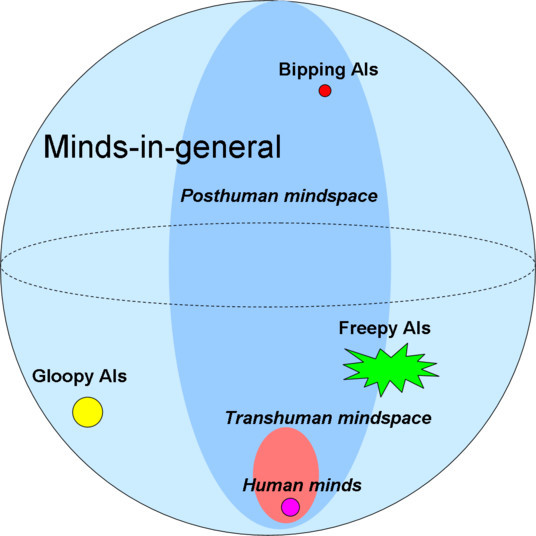
\includegraphics[scale=0.25]{Rationality20From20AI20to20Zombies2020Eliezer20Yudkowsky-img350.jpg}
 
\par}


\bigskip

{
\ \ \ ~}

{
\ \ \ All humans, of course, fit into a tiny little dot---as a sexually
reproducing species, we can't be too different from one
another.}

{
\ \ \ This tiny dot belongs to a wider ellipse, the space of transhuman
mind designs---things that might be smarter than us, or much smarter
than us, but that in some sense would still be people as we understand
people.}

{
\ \ \ This transhuman ellipse is within a still wider volume, the space
of posthuman minds, which is everything that a transhuman might grow up
into.}

{
\ \ \ And then the rest of the sphere is the space of minds-in-general,
including possible Artificial Intelligences so odd that they
aren't even \textit{posthuman.}}

{
\ \ \ But wait---natural selection designs complex artifacts and selects
among complex strategies. So where is natural selection on this map?}

{
\ \ \ So this entire map really floats in a still vaster space, the
space of optimization processes. At the bottom of this vaster space,
below even humans, is natural selection as it first began in some tidal
pool: mutate, replicate, and sometimes die, no sex.}

{
\ \ \ Are there any powerful optimization processes, with strength
comparable to a human civilization or even a self-improving AI, which
we would not recognize as minds? Arguably Marcus
Hutter's AIXI should go in this category: for a mind of
infinite power, it's awfully stupid---poor thing
can't even recognize itself in a mirror. But that is a
topic for another time.}

{
\ \ \ My primary moral is to \textit{resist the temptation to generalize
over all of mind design space}.}

{
\ \ \ If we focus on the bounded subspace of mind design space that
contains all those minds whose makeup can be specified in a trillion
bits or less, then every universal generalization that you make has two
to the trillionth power chances to be falsified.}

{
\ \ \ Conversely, every \textit{existential}
generalization---``there exists at least one mind such
that X''---has two to the trillionth power chances to
be true.}

{
\ \ \ So you want to resist the temptation to say either that
\textit{all} minds do something, or that \textit{no} minds do
something.}

{
\ \ \ The main reason you could find yourself thinking that you know
what a fully generic mind will (won't) do is if you put
yourself in that mind's shoes---imagine what you would
do in that mind's place---and get back a generally
wrong, anthropomorphic answer. (Albeit that it is true in at least one
case, since you are yourself an example.) Or if you imagine a mind
doing something, and then imagining the reasons \textit{you}
wouldn't do it---so that you imagine that a mind of
that type can't exist, that the ghost in the machine
will look over the corresponding source code and hand it back.}

{
\ \ \ Somewhere in mind design space is at least one mind with almost
any kind of logically consistent property you care to imagine.}

{
\ \ \ And this is important because it emphasizes the importance of
discussing \textit{what happens, lawfully, and why,} as a causal result
of a mind's particular constituent makeup; somewhere in
mind design space is a mind that does it differently.}

{
\ \ \ Of course, you could always say that anything that
doesn't do it your way is ``by
definition'' not a mind; after all,
it's obviously stupid. I've seen people
try that one too.}

{\centering
\ \ \ \ ~
\par}

{\centering
\ \ \ *
\par}

\chapter{Value Theory}

\mysection{Where Recursive Justification Hits Bottom}

{
\ \ \ Why do I believe that the Sun will rise tomorrow? }

{
\ \ \ Because I've seen the Sun rise on thousands of
previous days.}

{
\ \ \ Ah .~.~. but why do I believe the future will be like the past?}

{
\ \ \ Even if I go past the mere surface observation of the Sun rising,
to the apparently universal and exceptionless laws of gravitation and
nuclear physics, then I am still left with the question:
``Why do I believe this will also be true
tomorrow?''}

{
\ \ \ I could appeal to Occam's Razor, the principle of
using the simplest theory that fits the facts .~.~. but why believe in
Occam's Razor? Because it's been
successful on past problems? But who says that this means
Occam's Razor will work tomorrow?}

{
\ \ \ And lo, the one said:}

{
\ \ \ Science also depends on unjustified assumptions. Thus science is
ultimately based on faith, \textit{so don't you
criticize me} for believing in [silly-belief-\#238721].}

{
\ \ \ As I've previously observed:}

{
\ \ \ It's a most peculiar psychology---this business of
``Science is based on faith too, so
there!'' Typically this is said by people who claim
that faith is a \textit{good} thing. Then why do they say
``Science is based on faith too!''
in that angry-triumphal tone, rather than as a compliment?}

{
\ \ \ Arguing that you should be immune to criticism is rarely a good
sign.}

{
\ \ \ But this doesn't answer the legitimate
philosophical dilemma: If every belief must be justified, and those
justifications in turn must be justified, then how is the infinite
recursion terminated?}

{
\ \ \ And if you're allowed to end in something
assumed-without-justification, then why aren't you
allowed to assume \textit{any old thing} without justification?}

{
\ \ \ A similar critique is sometimes leveled against Bayesianism---that
it requires assuming some prior---by people who apparently think that
the problem of induction is a \textit{particular} problem of
Bayesianism, which you can avoid by using classical statistics.}

{
\ \ \ But first, let it be clearly admitted that the rules of Bayesian
updating do \textit{not} of themselves solve the problem of induction.}

{
\ \ \ Suppose you're drawing red and white balls from an
urn. You observe that, of the first 9 balls, 3 are red and 6 are white.
What is the probability that the next ball drawn will be red?}

{
\ \ \ That depends on your prior beliefs about the urn. If you think the
urn-maker generated a uniform random number between 0 and 1, and used
that number as the fixed probability of each ball being red, then the
answer is 4/11 (by Laplace's Law of Succession). If you
think the urn originally contained 10 red balls and 10 white balls,
then the answer is 7/11.}

{
\ \ \ Which goes to say that with the right prior---or rather the wrong
prior---the chance of the Sun rising tomorrow would seem to go
\textit{down} with each succeeding day .~.~. if you were absolutely
certain, a priori, that there was a great barrel out there from which,
on each day, there was drawn a little slip of paper that determined
whether the Sun rose or not; and that the barrel contained only a
limited number of slips saying
``Yes,'' and the slips were drawn
without replacement.}

{
\ \ \ There are possible minds in mind design space who have
anti-Occamian and anti-Laplacian priors; they believe that simpler
theories are less likely to be correct, and that the more often
something happens, the less likely it is to happen again.}

{
\ \ \ And when you ask these strange beings why they keep using priors
that never seem to work in real life .~.~. they reply,
``Because it's never worked for us
before!''}

{
\ \ \ Now, one lesson you might derive from this is
``Don't be born with a stupid
prior.'' This is an amazingly helpful principle on
many real-world problems, but I doubt it will satisfy philosophers.}

{
\ \ \ Here's how I treat this problem myself: I try to
approach questions like ``Should I trust my
brain?'' or ``Should I trust
Occam's Razor?'' as though they were
\textit{nothing special}{}---or at least, nothing special as deep
questions go.}

{
\ \ \ Should I trust Occam's Razor? Well, how well does
(any particular version of) Occam's Razor seem to work
in practice? What kind of probability-theoretic justifications can I
find for it? When I look at the universe, does it seem like the kind of
universe in which Occam's Razor would work well?}

{
\ \ \ Should I trust my brain? Obviously not; it doesn't
always work. But nonetheless, the human brain seems much more powerful
than the most sophisticated computer programs I could consider trusting
otherwise. How well does my brain work in practice, on which sorts of
problems?}

{
\ \ \ When I examine the causal history of my brain---its origins in
natural selection---I find, on the one hand, all sorts of specific
reasons for doubt; my brain was optimized to run on the ancestral
savanna, not to do math. But on the other hand, it's
also clear why, loosely speaking, it's possible that
the brain really could work. Natural selection would have quickly
eliminated brains so \textit{completely} unsuited to reasoning, so
\textit{anti-}helpful, as anti-Occamian or anti-Laplacian priors.}

{
\ \ \ So what I did in practice does \textit{not} amount to declaring a
sudden halt to questioning and justification. I'm not
halting the chain of examination at the point that I encounter
Occam's Razor, or my brain, or some other
unquestionable. The chain of examination continues---but it continues,
unavoidably, using my current brain and my current grasp on reasoning
techniques. \textit{What else could I possibly use?}}

{
\ \ \ Indeed, no matter \textit{what} I did with this dilemma, it would
be me doing it. Even if I trusted something else, like some computer
program, it would be my own decision to trust it.}

{
\ \ \ The technique of rejecting beliefs that have absolutely no
justification is in general an extremely important one. I sometimes say
that the fundamental question of rationality is ``Why
do you believe what you believe?'' I
don't even want to say something that \textit{sounds}
like it might allow a single exception to the rule that everything
needs justification.}

{
\ \ \ Which is, itself, a dangerous sort of motivation; you
can't always avoid everything that might be risky, and
when someone annoys you by saying something silly, you
can't reverse that stupidity to arrive at
intelligence.}

{
\ \ \ But I would nonetheless emphasize the difference between saying:}

{
\ \ \ Here is this assumption I cannot justify, which must be simply
taken, and not further examined.}

{
\ \ \ Versus saying:}

{
\ \ \ Here the inquiry continues to examine this assumption, with the
full force of my \textit{present intelligence}{}---as opposed to the
full force of something else, like a random number generator or a magic
8-ball---even though my present intelligence happens to be founded on
this assumption.}

{
\ \ \ Still .~.~. wouldn't it be nice if we could
examine the problem of how much to trust our brains \textit{without}
using our current intelligence? Wouldn't it be nice if
we could examine the problem of how to think, \textit{without} using
our current grasp of rationality?}

{
\ \ \ When you phrase it \textit{that} way, it starts looking like the
answer might be ``No.''}

{
\ \ \ E. T. Jaynes used to say that you must always use all the
information available to you---he was a Bayesian probability theorist,
and had to clean up the paradoxes other people generated when they used
different information at different points in their calculations. The
principle of ``\textit{Always put forth your true best
effort}'' has at least as much appeal as
``\textit{Never do anything that might look
circular.}'' After all, the alternative to putting
forth your best effort is presumably doing less than your best.}

{
\ \ \ \textit{But still} .~.~. wouldn't it be nice if
there were some way to justify using Occam's Razor, or
justify predicting that the future will resemble the past,
\textit{without} assuming that those methods of reasoning which have
worked on previous occasions are better than those which have
continually failed?}

{
\ \ \ Wouldn't it be nice if there were some chain of
justifications that neither ended in an unexaminable assumption, nor
was forced to examine itself under its own rules, but, instead, could
be explained starting from absolute scratch to an ideal philosophy
student of perfect emptiness?}

{
\ \ \ Well, I'd certainly be interested, but I
don't expect to see it done any time soon. There is no
perfectly empty ghost-in-the-machine; there is no argument that you can
explain to a rock.}

{
\ \ \ Even if someone cracks the First Cause problem and comes up with
\textit{the actual reason the universe is simple, which does not itself
presume a simple universe .~.~.} then I would still expect that the
explanation could only be understood by a mindful listener, and not by,
say, a rock. A listener that didn't start out already
implementing modus ponens might be out of luck.}

{
\ \ \ So, at the end of the day, what happens when someone keeps asking
me ``Why do you believe what you
believe?''}

{
\ \ \ At present, I start going around in a loop at the point where I
explain, ``I predict the future as though it will
resemble the past on the simplest and most stable level of organization
I can identify, because previously, this rule has usually worked to
generate good results; and using the simple assumption of a simple
universe, I can see \textit{why} it generates good results; and I can
even see how my brain might have evolved to be able to observe the
universe with some degree of accuracy, if my observations are
correct.''}

{
\ \ \ But then .~.~. haven't I just licensed
\textit{circular logic}?}

{
\ \ \ Actually, I've just licensed \textit{reflecting on
your mind's degree of trustworthiness, using your
current mind as opposed to something else.}}

{
\ \ \ Reflection of this sort is, indeed, the reason we reject most
circular logic in the first place. We want to have a coherent causal
story about how our mind comes to know something, a story that explains
how the process we used to arrive at our beliefs is itself trustworthy.
This is the essential demand behind the rationalist's
fundamental question, ``Why do you believe what you
believe?''}

{
\ \ \ Now suppose you write on a sheet of paper: ``(1)
Everything on this sheet of paper is true, (2) The mass of a helium
atom is 20 grams.'' If that trick actually
\textit{worked in real life}, you would be able to know the true mass
of a helium atom just by believing some circular logic that asserted
it. Which would enable you to arrive at a true map of the universe
sitting in your living room with the blinds drawn. Which would violate
the Second Law of Thermodynamics by generating information from
nowhere. Which would not be a plausible story about how your mind could
end up believing something true.}

{
\ \ \ \textit{Even if} you started out believing the sheet of paper, it
would not seem that you had any reason for why the paper corresponded
to reality. It would just be a miraculous coincidence that (a) the mass
of a helium atom was 20 grams, and (b) the paper happened to say so.}

{
\ \ \ Believing self-validating statement sets does not in general seem
like it should work to map external reality---when we \textit{reflect
on it as a causal story about minds}{}---using, of course, our
\textit{current} minds to do so.}

{
\ \ \ But what about evolving to give more credence to simpler beliefs,
and to believe that algorithms which have worked in the past are more
likely to work in the future? \textit{Even when} we reflect on this as
a causal story of the origin of minds, it still seems like this could
plausibly work to map reality.}

{
\ \ \ And what about trusting reflective coherence in general?
Wouldn't most possible minds, randomly generated and
allowed to settle into a state of reflective coherence, be incorrect?
Ah, but \textit{we} evolved by natural selection; we were not generated
randomly.}

{
\ \ \ If trusting this argument seems worrisome to you, then forget
about the problem of philosophical justifications, and ask yourself
whether it's really truly true.}

{
\ \ \ (You will, of course, use your own mind to do so.)}

{
\ \ \ Is this the same as the one who says, ``I believe
that the Bible is the word of God, because the Bible says
so''?}

{
\ \ \ Couldn't they argue that their blind faith must
also have been placed in them by God, and is therefore trustworthy?}

{
\ \ \ In point of fact, when religious people finally come to reject the
Bible, they do \textit{not} do so by magically jumping to a
non-religious state of pure emptiness, and then evaluating their
religious beliefs in that non-religious state of mind, and then jumping
back to a new state with their religious beliefs removed.}

{
\ \ \ People go from being religious to being non-religious because even
in a religious state of mind, doubt seeps in. They notice their prayers
(and worse, the prayers of seemingly much worthier people) are not
being answered. They notice that God, who speaks to them in their heart
in order to provide seemingly consoling answers about the universe, is
not able to tell them the hundredth digit of pi (which would be a lot
more reassuring, if God's purpose were reassurance).
They examine the story of God's creation of the world
and damnation of unbelievers, and it doesn't seem to
make sense even under their own religious premises.}

{
\ \ \ Being religious doesn't make you less than human.
Your brain still has the abilities of a human brain. The dangerous part
is that being religious might stop you from \textit{applying} those
native abilities to your religion---stop you from \textit{reflecting
fully} on yourself. People don't heal their errors by
resetting themselves to an ideal philosopher of pure emptiness and
reconsidering all their sensory experiences from scratch. They heal
themselves by becoming more willing to question their current beliefs,
using more of the power of their current mind.}

{
\ \ \ This is why it's important to distinguish between
\textit{reflecting on your mind using your mind} (it's
not like you can use anything else) and \textit{having an
unquestionable assumption that you can't reflect on.}}

{
\ \ \ ``I believe that the Bible is the word of God,
because the Bible says so.'' Well, if the Bible
\textit{were} an astoundingly reliable source of information about all
other matters, if it had not said that grasshoppers had four legs or
that the universe was created in six days, but had instead contained
the Periodic Table of Elements centuries before chemistry---if the
Bible had served us only well and told us only truth---then we might,
in fact, be inclined to take seriously the additional statement in the
Bible, that the Bible had been generated by God. We might not trust it
entirely, because it could also be aliens or the Dark Lords of the
Matrix, but it would at least be worth taking seriously.}

{
\ \ \ Likewise, if everything \textit{else} that priests had told us
turned out to be true, we might take more seriously their statement
that faith had been placed in us by God and was a systematically
trustworthy source---especially if people could divine the hundredth
digit of pi by faith as well.}

{
\ \ \ So the important part of appreciating the circularity of
``I believe that the Bible is the word of God, because
the Bible says so,'' is not so much that you are
going to reject the idea of reflecting on your mind using your current
mind. Rather, you realize that anything which calls into question the
Bible's trustworthiness also calls into question the
Bible's assurance of its trustworthiness.}

{
\ \ \ This applies to rationality too: if the future should cease to
resemble the past---even on its lowest and simplest and most stable
observed levels of organization---well, mostly, I'd be
dead, because my brain's processes require a lawful
universe where chemistry goes on working. But if somehow I survived,
then I would have to start questioning the principle that the future
should be predicted to be like the past.}

{
\ \ \ But for now .~.~. what's the \textit{alternative}
to saying, ``I'm going to believe that
the future will be like the past on the most stable level of
organization I can identify, because that's previously
worked better for me than any other algorithm I've
tried''?}

{
\ \ \ Is it saying, ``I'm going to
believe that the future will \textit{not} be like the past, because
that algorithm has always failed before''?}

{
\ \ \ At this point I feel obliged to drag up the point that
rationalists are not out to win arguments with ideal philosophers of
perfect emptiness; we are simply out to win. For which purpose we want
to get as close to the truth as we can possibly manage. So at the end
of the day, I embrace the principle: ``Question your
brain, question your intuitions, question your principles of
rationality, \textit{using the full current force of your mind, and
doing the best you can do at every point.}''}

{
\ \ \ If one of your current principles does come up wanting---according
to your own mind's examination, since you
can't step outside yourself{}---then change it! And
then go back and look at things again, using your new improved
principles.}

{
\ \ \ The point is not to be reflectively consistent. The point is to
win. But \textit{if} you look at yourself and play to win, you are
making yourself more reflectively consistent---that's
what it means to ``play to win''
while ``looking at yourself.''}

{
\ \ \ Everything, without exception, needs justification.
Sometimes---unavoidably, as far as I can tell---those justifications
will go around in reflective loops. I do think that reflective loops
have a meta-character which should enable one to distinguish them, by
common sense, from circular logics. But anyone seriously considering a
circular logic in the first place is probably out to lunch in matters
of rationality, and will simply insist that their circular logic is a
``reflective loop'' even if it
consists of a single scrap of paper saying ``Trust
me.'' Well, you can't always optimize
your rationality techniques according to the sole consideration of
preventing those bent on self-destruction from abusing them.}

{
\ \ \ The important thing is to \textit{hold nothing back} in your
criticisms of how to criticize; nor should you regard the
unavoidability of loopy justifications as a warrant of \textit{immunity
from questioning}.}

{
\ \ \ Always apply full force, whether it loops or not---do the best you
can possibly do, whether it loops or not---and play, ultimately, to
win.}

{\centering
\ \ \ \ ~
\par}

{\centering
\ \ \ *
\par}

\mysection{My Kind of Reflection}

{
\ \ \ In Where Recursive Justification Hits Bottom, I concluded that
it's okay to use induction to reason about the
probability that induction will work in the future, given that
it's worked in the past; or to use
Occam's Razor to conclude that the simplest explanation
for why Occam's Razor works is that the universe itself
is fundamentally simple. }

{
\ \ \ Now I am far from the first person to consider reflective
application of reasoning principles. Chris Hibbert compared my view to
Bartley's Pan-Critical Rationalism (I was wondering
whether that would happen). So it seems worthwhile to state what I see
as the distinguishing features of my view of reflection, which may or
may not happen to be shared by any other philosopher's
view of reflection.}

{
\ \ \ All of my philosophy here \textit{actually} comes from trying to
figure out how to build a self-modifying AI that applies its own
reasoning principles to itself in the process of rewriting its own
source code. So whenever I talk about using induction to license
induction, I'm \textit{really} thinking about an
inductive AI considering a rewrite of the part of itself that performs
induction. If you wouldn't want the AI to rewrite its
source code to not use induction, your philosophy had better not label
induction as unjustifiable.}

{
\ \ \ One of the most powerful principles I know for AI in general is
that the true Way generally turns out to be
\textit{naturalistic}{}---which for reflective reasoning means treating
transistors inside the AI just as if they were transistors found in the
environment, \textit{not} an ad-hoc special case. This is the real
source of my insistence in Recursive Justification that questions like
``How well does my version of Occam's
Razor work?'' should be considered just like an
ordinary question---or at least an ordinary very deep question. I
strongly suspect that a correctly built AI, in pondering modifications
to the part of its source code that implements Occamian reasoning, will
not have to do anything special as it ponders---in particular, it
shouldn't have to make a special effort to avoid using
Occamian reasoning.}

{
\ \ \ I don't think that ``reflective
coherence'' or ``reflective
consistency'' should be considered as a desideratum
in itself. As I say in The Twelve Virtues and The Simple Truth, if you
make five accurate maps of the same city, then the maps will
necessarily be consistent with each other; but if you draw one map by
fantasy and then make four copies, the five will be consistent but not
accurate. In the same way, no one is deliberately pursuing reflective
consistency, and reflective consistency is not a special warrant of
trustworthiness; the goal is to win. But anyone who pursues the goal of
winning, using their current notion of winning, and modifying their own
source code, will end up reflectively consistent as a side
effect---just like someone continually striving to improve their map of
the world should find the parts becoming more consistent among
themselves, as a side effect. If you put on your AI goggles, then the
AI, rewriting its own source code, is not trying to make itself
``reflectively consistent''---it is
trying to optimize the expected utility of its source code, and it
happens to be doing this using its current mind's
anticipation of the consequences.}

{
\ \ \ One of the ways I license using induction and
Occam's Razor to consider
``induction'' and
``Occam's Razor'' is
by appealing to E. T. Jaynes's principle that we should
always use all the information available to us (computing power
permitting) in a calculation. If you think induction works, then you
should use it in order to use your maximum power, including when
you're thinking about induction.}

{
\ \ \ In general, I think it's valuable to distinguish a
defensive posture where you're imagining how to justify
your philosophy to a philosopher that questions you, from an aggressive
posture where you're trying to get as close to the
truth as possible. So it's not that being suspicious of
Occam's Razor, but using your current mind and
intelligence to inspect it, shows that you're being
\textit{fair} and \textit{defensible} by questioning your foundational
beliefs. Rather, the reason why you would inspect
Occam's Razor is to see if you could improve your
application of it, or if you're worried it might really
be wrong. I tend to deprecate mere dutiful doubts.}

{
\ \ \ If you run around inspecting your foundations, I expect you to
actually improve them, not just dutifully investigate. Our brains are
built to assess ``simplicity'' in a
certain intuitive way that makes Thor sound simpler than
Maxwell's Equations as an explanation for lightning.
But, having gotten a better look at the way the universe really works,
we've concluded that differential equations (which few
humans master) are actually \textit{simpler} (in an
information-theoretic sense) than heroic mythology (which is how most
tribes explain the universe). This being the case,
we've tried to import our notions of
Occam's Razor into math as well.}

{
\ \ \ On the other hand, the improved foundations should still add up to
normality; 2 + 2 should still end up equalling 4, not something new and
amazing and exciting like ``fish.''}

{
\ \ \ I think it's very important to distinguish between
the questions ``Why does induction
work?'' and ``Does induction
work?'' The reason \textit{why the universe itself is
regular} is still a mysterious question unto us, for now. Strange
speculations here may be temporarily needful. But on the other hand, if
you start claiming that the universe \textit{isn't
actually regular}, that the answer to ``Does induction
work?'' is
``No!,'' then you're
wandering into 2 + 2 = 3 territory. You're trying too
hard to make your philosophy interesting, instead of correct. An
inductive AI asking what probability assignment to make on the next
round is asking ``\textit{Does} induction
work?,'' and this is the question that it may answer
by inductive reasoning. If you ask ``\textit{Why} does
induction work?'' then answering
``Because induction works'' is
circular logic, and answering ``Because I believe
induction works'' is magical thinking.}

{
\ \ \ I don't think that going around in a loop of
justifications through the meta-level is the same thing as circular
logic. I think the notion of ``circular
logic'' applies within the object level, and is
something that is definitely bad and forbidden, on the object level.
Forbidding \textit{reflective coherence} doesn't sound
like a good idea. But I haven't yet sat down and
formalized the exact difference---my reflective theory is something
I'm trying to work out, not something I have in hand.}

{\centering
\ \ \ \ ~
\par}

{\centering
\ \ \ *
\par}

\mysection{No Universally Compelling Arguments}

{
\ \ \ What is so \textit{terrifying} about the idea that not every
possible mind might agree with us, even in principle? }

{
\ \ \ For some folks, nothing---it doesn't bother them
in the slightest. And for some of \textit{those} folks, the
\textit{reason} it doesn't bother them is that they
don't have strong intuitions about standards and truths
that go beyond personal whims. If they say the sky is blue, or that
murder is wrong, that's just their personal opinion;
and that someone else might have a different opinion
doesn't surprise them.}

{
\ \ \ For other folks, a disagreement that persists even \textit{in
principle} is something they can't accept. And for some
of \textit{those} folks, the \textit{reason} it bothers them is that it
seems to them that if you allow that some people cannot be persuaded
\textit{even in principle} that the sky is blue, then
you're conceding that ``the sky is
blue'' is merely an \textit{arbitrary} personal
opinion.}

{
\ \ \ I've proposed that you should resist the
temptation to generalize over all of mind design space. If we restrict
ourselves to minds specifiable in a trillion bits or less, then each
\textit{universal} generalization ``All minds m:
X(m)'' has two to the trillionth chances to be false,
while each \textit{existential} generalization
``Exists mind m: X(m)'' has two to
the trillionth chances to be true.}

{
\ \ \ This would seem to argue that for every argument A, howsoever
convincing it may seem to us, there exists at least one possible mind
that doesn't buy it.}

{
\ \ \ And the surprise and/or horror of this prospect (for some) has a
great deal to do, I think, with the intuition of the
ghost-in-the-machine---a ghost with some irreducible core that any
\textit{truly valid} argument will convince.}

{
\ \ \ I have previously spoken of the intuition whereby people map
\textit{programming a computer} onto \textit{instructing a human
servant}, so that the computer might rebel against its code---or
perhaps look over the code, decide it is not reasonable, and hand it
back.}

{
\ \ \ If there were a ghost in the machine and the ghost contained an
irreducible core of reasonableness, above which any mere code was only
a suggestion, then there might be universal arguments. Even if the
ghost were initially handed code-suggestions that contradicted the
Universal Argument, when we finally did expose the ghost to the
Universal Argument---or the ghost could discover the Universal Argument
on its own, that's also a popular concept---the ghost
would just override its own, mistaken source code.}

{
\ \ \ But as the student programmer once said, ``I get
the feeling that the computer just skips over all the
comments.'' The code is not given to the AI; the code
\textit{is} the AI.}

{
\ \ \ If you switch to the physical perspective, then the notion of a
Universal Argument seems noticeably unphysical. If
there's a physical system that at time T, after being
exposed to argument E, does X, then there ought to be another physical
system that at time T, after being exposed to environment E, does Y.
Any thought has to be implemented \textit{somewhere}, in a physical
system; any belief, any conclusion, any decision, any motor output. For
every lawful causal system that zigs at a set of points, you should be
able to specify another causal system that lawfully zags at the same
points.}

{
\ \ \ Let's say there's a mind with a
transistor that outputs +3 volts at time T, indicating that it has just
assented to some persuasive argument. Then we can build a highly
similar physical cognitive system with a tiny little trapdoor
underneath the transistor containing a little gray man who climbs out
at time T and sets that transistor's output to -3
volts, indicating non-assent. Nothing acausal about that; the little
gray man is there because we built him in. The notion of an argument
that convinces \textit{any} mind seems to involve a little blue woman
who was \textit{never} built into the system, who climbs out of
literally \textit{nowhere}, and strangles the little gray man, because
that transistor has just \textit{got} to output +3 volts.
It's such a \textit{compelling argument}, you see.}

{
\ \ \ But compulsion is not a property of arguments; it is a property of
minds that process arguments.}

{
\ \ \ So the reason I'm arguing against the ghost
isn't \textit{just} to make the point that (1) Friendly
AI has to be explicitly programmed and (2) the laws of physics do not
forbid Friendly AI. (Though of course I take a certain interest in
establishing this.)}

{
\ \ \ I also wish to establish the notion of a mind as a \textit{causal,
lawful, physical system} in which there \textit{is no} irreducible
central ghost that looks over the neurons/code and decides whether they
are good suggestions.}

{
\ \ \ (There is a concept in Friendly AI of \textit{deliberately}
programming an FAI to review its own source code and possibly hand it
back to the programmers. But the mind that reviews is not irreducible,
it is just the mind that you created. The FAI is renormalizing itself
\textit{however it was designed to do so}; there is nothing acausal
reaching in from outside. A bootstrap, not a skyhook.)}

{
\ \ \ All this echoes back to the worry about a
Bayesian's
``arbitrary'' priors. If you show me
one Bayesian who draws 4 red balls and 1 white ball from a barrel, and
who assigns probability 5/7 to obtaining a red ball on the next
occasion (by Laplace's Rule of Succession), then I can
show you another mind which obeys Bayes's Rule to
conclude a 2/7 probability of obtaining red on the next
occasion---corresponding to a different prior belief about the barrel,
but, perhaps, a less ``reasonable''
one.}

{
\ \ \ Many philosophers are convinced that because you can in-principle
construct a prior that updates to any given conclusion on a stream of
evidence, therefore, Bayesian reasoning must be
``arbitrary,'' and the whole schema
of Bayesianism flawed, because it relies on
``unjustifiable'' assumptions, and
indeed ``unscientific,'' because you
cannot force any possible journal editor in mindspace to agree with
you.}

{
\ \ \ And this (I replied) relies on the notion that by unwinding all
arguments and their justifications, you can obtain an ideal philosophy
student of perfect emptiness, to be convinced by a line of reasoning
that begins from absolutely no assumptions.}

{
\ \ \ But who is this ideal philosopher of perfect emptiness? Why, it is
just the irreducible core of the ghost!}

{
\ \ \ And that is why (I went on to say) the result of trying to remove
all assumptions from a mind, and unwind to the perfect absence of any
prior, is not an ideal philosopher of perfect emptiness, but a rock.
What is left of a mind after you remove the source code? Not the ghost
who looks over the source code, but simply .~.~. no ghost.}

{
\ \ \ So---and I shall take up this theme again later---wherever you are
to locate your notions of \textit{validity} or \textit{worth} or
\textit{rationality} or \textit{justification} or even
\textit{objectivity}, it cannot rely on an argument that is
\textit{universally compelling to all physically possible minds.}}

{
\ \ \ Nor can you ground validity in a sequence of justifications that,
beginning from nothing, persuades a perfect emptiness.}

{
\ \ \ Oh, there might be argument sequences that would compel any
neurologically intact \textit{human}{}---like the argument I use to
make people let the AI out of the box\textsuperscript{1}{}---but that
is hardly the same thing from a philosophical perspective.}

{
\ \ \ The first great failure of those who try to consider Friendly AI
is the One Great Moral Principle That Is All We Need To
Program---a.k.a. the fake utility function---and of this I have already
spoken.}

{
\ \ \ But the even worse failure is the One Great Moral Principle We
Don't Even \textit{Need} To Program Because Any AI Must
Inevitably Conclude It. This notion exerts a terrifying unhealthy
fascination on those who spontaneously reinvent it; they dream of
commands that no sufficiently advanced mind can disobey. The gods
themselves will proclaim the rightness of their philosophy! (E.g., John
C. Wright, Marc Geddes.)}

{
\ \ \ There is also a less severe version of the failure, where the one
does not \textit{declare} the One True Morality. Rather the one hopes
for an AI created \textit{perfectly free}, unconstrained by flawed
humans desiring slaves, so that the AI may arrive at virtue of its own
accord---virtue undreamed-of perhaps by the speaker, who confesses
themselves too flawed to teach an AI. (E.g., John K. Clark, Richard
Hollerith?, Eliezer\textsubscript{1996}.) This is a less tainted motive
than the dream of absolute command. But though \textit{this} dream
arises from virtue rather than vice, it is still based on a flawed
understanding of freedom, and will not actually \textit{work in real
life.} Of this, more to follow, of course.}

{
\ \ \ John C. Wright, who was previously writing a very nice
transhumanist trilogy (first book: \textit{The Golden Age}), inserted a
huge Author Filibuster in the middle of his climactic third book,
describing in tens of pages his Universal Morality That Must Persuade
Any AI. I don't know if anything happened after that,
because I stopped reading. And then Wright converted to
Christianity---yes, seriously. So you \textit{really
don't} want to fall into this trap!}

{\centering
\ \ \ \ ~
\par}

{\centering
\ \ \ *
\par}


\bigskip

{
\ \ \ 1. Just kidding.}

\mysection{Created Already in Motion}

{
\ \ \ Lewis Carroll, who was also a mathematician, once wrote a short
dialogue called ``What the Tortoise said to
Achilles.'' If you have not yet read this ancient
classic, consider doing so now. }

{
\ \ \ The Tortoise offers Achilles a step of reasoning drawn from
Euclid's First Proposition:}

{
\ \ \ (A) Things that are equal to the same are equal to each other.}

{
\ \ \ (B) The two sides of this Triangle are things that are equal to
the same.}

{
\ \ \ (Z) The two sides of this Triangle are equal to each other.}

{
\ \ \ Tortoise: ``And if some reader had \textit{not}
yet accepted A and B as true, he might still accept the
\textit{sequence} as a \textit{valid} one, I
suppose?''}

{
\ \ \ Achilles: ``No doubt such a reader might exist.
He might say, `I accept as true the Hypothetical
Proposition that, \textit{if} A and B be true, Z must be true; but, I
\textit{don't} accept A and B as true.'
Such a reader would do wisely in abandoning Euclid, and taking to
football.''}

{
\ \ \ Tortoise: ``And might there not \textit{also} be
some reader who would say, `I accept A and B as true,
but I \textit{don't} accept the
Hypothetical'?''}

{
\ \ \ Achilles, unwisely, concedes this; and so asks the Tortoise to
accept another proposition:}

{
\ \ \ (C) If A and B are true, Z must be true.}

{
\ \ \ But, asks, the Tortoise, suppose that he accepts A and B and C,
but not Z?}

{
\ \ \ Then, says, Achilles, he must ask the Tortoise to accept one more
hypothetical:}

{
\ \ \ (D) If A and B and C are true, Z must be true.}

{
\ \ \ Douglas Hofstadter paraphrased the argument some time later:}

{
\ \ \ ACHILLES: ``If you have [(A and B) $\rightarrow $
Z], and you also have (A and B), then surely you have
Z.''}

{
\ \ \ TORTOISE: ``Oh! You mean ((A and B) and [(A and
B) $\rightarrow $ Z]) $\rightarrow $ Z, don't
you?''}

{
\ \ \ As Hofstadter says, ``Whatever Achilles considers
a rule of inference, the Tortoise immediately flattens into a mere
string of the system. If you use only the letters A, B, and Z, you will
get a recursive pattern of longer and longer
strings.''}

{
\ \ \ This is the anti-pattern I call Passing the Recursive Buck; and
though the counterspell is sometimes hard to find, when found, it
generally takes the form The Buck Stops Immediately.}

{
\ \ \ The Tortoise's mind needs the \textit{dynamic} of
adding Y to the belief pool when X and (X $\rightarrow $ Y) are
previously in the belief pool. If this dynamic is not present---a rock,
for example, lacks it---then you can go on adding in X and (X
$\rightarrow $ Y) and ((X and (X $\rightarrow $ Y)) $\rightarrow $ Y)
until the end of eternity, without ever getting to Y.}

{
\ \ \ The phrase that once came into my mind to describe this
requirement is that a mind must be \textit{created already in motion.}
There is no argument so compelling that it will give dynamics to a
static thing. There is no computer program so \textit{persuasive} that
you can run it on a rock.}

{
\ \ \ And even if you have a mind that \textit{does} carry out modus
ponens, it is futile for it to have such beliefs as .~.~.}

{
\ \ \ (A) If a toddler is on the train tracks, then pulling them off is
fuzzle.}

{
\ \ \ (B) There is a toddler on the train tracks.}

{
\ \ \ .~.~. unless the mind also \textit{implements}:}

{
\ \ \ \textit{Dynamic:} When the belief pool contains
``X is fuzzle,'' send X to the
action system.}

{
\ \ \ By ``dynamic'' I mean a
property of a physically implemented cognitive system's
\textit{development over time}. A
``dynamic'' is something that
\textit{happens inside} a cognitive system, \textit{not} data that it
stores in memory and manipulates. Dynamics are the manipulations. There
is no way to write a dynamic on a piece of paper, because the paper
will just lie there. So the text immediately above, which says
``dynamic,'' is not dynamic. If I
wanted the text to \textit{be} dynamic and not just \textit{say}
``dynamic,'' I would have to write a
Java applet.}

{
\ \ \ Needless to say, having the belief .~.~.}

{
\ \ \ (C) If the belief pool contains ``X is
fuzzle,'' then ``send
`X' to the action
system'' is fuzzle.}

{
\ \ \ .~.~. won't help unless the mind already
implements the \textit{behavior} of translating hypothetical actions
labeled ``fuzzle'' into actual motor
actions.}

{
\ \ \ By dint of careful arguments about the nature of cognitive
systems, you might be able to prove .~.~.}

{
\ \ \ (D) A mind with a dynamic that sends plans labeled
``fuzzle'' to the action system is
more fuzzle than minds that don't.}

{
\ \ \ .~.~. but that \textit{still} won't help, unless
the listening mind \textit{previously} possessed the \textit{dynamic}
of swapping out its current source code for alternative source code
that is believed to be more fuzzle.}

{
\ \ \ This is why you can't argue fuzzleness into a
rock.}

{\centering
\ \ \ \ ~
\par}

{\centering
\ \ \ *
\par}

\mysection{Sorting Pebbles into Correct Heaps}

{
\ \ \ Once upon a time there was a strange little species---that might
have been biological, or might have been synthetic, and perhaps were
only a dream---whose passion was sorting pebbles into correct heaps. }

{
\ \ \ They couldn't tell you \textit{why} some heaps
were correct, and some incorrect. But all of them agreed that the most
important thing in the world was to create correct heaps, and scatter
incorrect ones.}

{
\ \ \ Why the Pebblesorting People cared so much, is lost to this
history---maybe a Fisherian runaway sexual selection, started by sheer
accident a million years ago? Or maybe a strange work of sentient art,
created by more powerful minds and abandoned?}

{
\ \ \ But it mattered so drastically to them, this sorting of pebbles,
that all the Pebblesorting philosophers said in unison that
pebble-heap-sorting was the very meaning of their lives: and held that
the only justified reason to eat was to sort pebbles, the only
justified reason to mate was to sort pebbles, the only justified reason
to participate in their world economy was to efficiently sort pebbles.}

{
\ \ \ The Pebblesorting People all agreed on that, but they
didn't always agree on which heaps were correct or
incorrect.}

{
\ \ \ In the early days of Pebblesorting civilization, the heaps they
made were mostly small, with counts like 23 or 29; they
couldn't tell if larger heaps were correct or not.
Three millennia ago, the Great Leader Biko made a heap of 91 pebbles
and proclaimed it correct, and his legions of admiring followers made
more heaps likewise. But over a handful of centuries, as the power of
the Bikonians faded, an intuition began to accumulate among the
smartest and most educated that a heap of 91 pebbles was incorrect.
Until finally they came to know what they had done: and they scattered
all the heaps of 91 pebbles. Not without flashes of regret, for some of
those heaps were great works of art, but incorrect. They even scattered
Biko's original heap, made of 91 precious gemstones
each of a different type and color.}

{
\ \ \ And no civilization since has seriously doubted that a heap of 91
is incorrect.}

{
\ \ \ Today, in these wiser times, the size of the heaps that
Pebblesorters dare attempt has grown very much larger---which all agree
would be a most great and excellent thing, if only they could ensure
the heaps were really \textit{correct.} Wars have been fought between
countries that disagree on which heaps are correct: the Pebblesorters
will never forget the Great War of 1957, fought between
Y'ha-nthlei and
Y'not'ha-nthlei, over heaps of size
1957. That war, which saw the first use of nuclear weapons on the
Pebblesorting Planet, finally ended when the
Y'not'ha-nthleian philosopher
At'gra'len'ley
exhibited a heap of 103 pebbles and a heap of 19 pebbles side-by-side.
So persuasive was this argument that even Y'ha-nthlei
reluctantly conceded that it was best to stop building heaps of 1957
pebbles, at least for the time being.}

{
\ \ \ Since the Great War of 1957, countries have been reluctant to
openly endorse or condemn heaps of large size, since this leads so
easily to war. Indeed, some Pebblesorting philosophers---who seem to
take a tangible delight in shocking others with their cynicism---have
entirely denied the existence of pebble-sorting \textit{progress}; they
suggest that opinions about pebbles have simply been a random walk over
time, with no coherence to them, the illusion of progress created by
condemning all dissimilar pasts as incorrect. The philosophers point to
the disagreement over pebbles of large size, as proof that there is
nothing that makes a heap of size 91 really \textit{incorrect}{}---that
it was simply fashionable to build such heaps at one point in time, and
then at another point, fashionable to condemn them.
``But .~.~. 13!'' carries no truck
with them; for to regard ``13!'' as
a persuasive counterargument is only another convention, they say. The
Heap Relativists claim that their philosophy may help prevent future
disasters like the Great War of 1957, but it is widely considered to be
a philosophy of despair.}

{
\ \ \ Now the question of what makes a heap correct or incorrect has
taken on new urgency; for the Pebblesorters may shortly embark on the
creation of self-improving Artificial Intelligences. The Heap
Relativists have warned against this project: They say that AIs, not
being of the species \textit{Pebblesorter sapiens}, may form their own
culture with entirely different ideas of which heaps are correct or
incorrect. ``They could decide that heaps of 8 pebbles
are correct,'' say the Heap Relativists,
``and while ultimately they'd be no
righter or wronger than us, still, \textit{our} civilization says we
shouldn't build such heaps. It is not in our interest
to create AI, unless all the computers have bombs strapped to them, so
that even if the AI thinks a heap of 8 pebbles is correct, we can force
it to build heaps of 7 pebbles instead. Otherwise,
KABOOM!''}

{
\ \ \ But this, to most Pebblesorters, seems absurd. Surely a
sufficiently powerful AI---especially the
``superintelligence'' some
transpebblesorterists go on about---would be able to see \textit{at a
glance} which heaps were correct or incorrect! The thought of something
with a brain the size of a planet thinking that a heap of 8 pebbles was
correct is just too absurd to be worth talking about.}

{
\ \ \ Indeed, it is an utterly futile project to constrain how a
superintelligence sorts pebbles into heaps. Suppose that Great Leader
Biko had been able, in his primitive era, to construct a self-improving
AI; and he had built it as an expected utility maximizer whose utility
function told it to create as many heaps as possible of size 91.
Surely, when this AI improved itself far enough, and became smart
enough, then it would see at a glance that this utility function was
incorrect; and, having the ability to modify its own source code, it
would \textit{rewrite its utility function} to value more reasonable
heap sizes, like 101 or 103.}

{
\ \ \ And certainly not heaps of size 8. That would just be
\textit{stupid.} Any mind that stupid is too dumb to be a threat.}

{
\ \ \ Reassured by such common sense, the Pebblesorters pour full speed
ahead on their project to throw together lots of algorithms at random
on big computers until some kind of intelligence emerges. The whole
history of civilization has shown that richer, smarter, better educated
civilizations are likely to agree about heaps that their ancestors once
disputed. Sure, there are then larger heaps to argue about---but the
further technology has advanced, the larger the heaps that have been
agreed upon and constructed.}

{
\ \ \ Indeed, intelligence itself has always correlated with making
correct heaps---the nearest evolutionary cousins to the Pebblesorters,
the Pebpanzees, make heaps of only size 2 or 3, and occasionally stupid
heaps like 9. And other, even less intelligent creatures, like fish,
make no heaps at all.}

{
\ \ \ Smarter minds equal smarter heaps. Why would that trend break?}

{\centering
\ \ \ \ ~
\par}

{\centering
\ \ \ *
\par}

\mysection{2{}-Place and 1{}-Place Words}

{
\ \ \ I have previously spoken of the ancient, pulp-era magazine covers
that showed a bug-eyed monster carrying off a girl in a torn dress; and
about how people think as if sexiness is an inherent property of a sexy
entity, without dependence on the admirer. }

{
\ \ \ ``Of \textit{course} the bug-eyed monster will
prefer human females to its own kind,'' says the
artist (who we'll call Fred); ``it can
see that human females have soft, pleasant skin instead of slimy
scales. It may be an alien, but it's not
\textit{stupid}{}---why are you expecting it to make such a basic
mistake about sexiness?''}

{
\ \ \ What is Fred's error? It is treating a function of
2 arguments (``2-place function''):}

{\centering
\ \ \ Sexiness: Admirer, Entity $\rightarrow $ [0,${\infty}$),
\par}


\bigskip

{
\ \ \ as though it were a function of 1 argument
(``1-place function''):}

{\centering
\ \ \ Sexiness: Entity $\rightarrow $ [0,${\infty}$).
\par}


\bigskip

{
\ \ \ If Sexiness is treated as a function that accepts only one Entity
as its argument, then of course Sexiness will appear to depend only on
the Entity, with nothing else being relevant.}

{
\ \ \ When you think about a two-place function as though it were a
one-place function, you end up with a Variable Question Fallacy / Mind
Projection Fallacy. Like trying to determine whether a building is
\textit{intrinsically} on the left or on the right side of the road,
independent of anyone's travel direction.}

{
\ \ \ An alternative and equally valid standpoint is that
``sexiness'' \textit{does} refer to
a one-place function---but each speaker uses a \textit{different}
one-place function to decide who to kidnap and ravish. Who says that
just because Fred, the artist, and Bloogah, the bug-eyed monster, both
use the word ``sexy,'' they must
mean the same thing by it?}

{
\ \ \ If you take this viewpoint, there is no paradox in speaking of
some woman intrinsically having 5 units of Fred::Sexiness. All
onlookers can agree on this fact, once Fred::Sexiness has been
specified in terms of curves, skin texture, clothing, status cues, etc.
This specification need \textit{make no mention of Fred}, only the
woman to be evaluated.}

{
\ \ \ It so happens that Fred, himself, \textit{uses} this algorithm to
select flirtation targets. But that doesn't mean the
algorithm itself has to \textit{mention} Fred. So
Fred's Sexiness function really \textit{is} a function
of one argument---the woman---on this view. I called it Fred::Sexiness,
but remember that this \textit{name} refers to a function that is being
described independently of Fred. Maybe it would be better to write:}

{\centering
\ \ \ Fred::Sexiness == Sexiness\_20934.
\par}


\bigskip

{
\ \ \ It is an empirical fact about Fred that he uses the function
Sexiness\_20934 to evaluate potential mates. Perhaps John uses exactly
the same algorithm; it doesn't matter where it comes
from once we have it.}

{
\ \ \ And similarly, the same woman has only 0.01 units of
Sexiness\_72546, whereas a slime mold has 3 units of Sexiness\_72546.
It happens to be an empirical fact that Bloogah uses Sexiness\_72546 to
decide who to kidnap; that is, Bloogah::Sexiness names the fixed
Bloogah-independent mathematical object that is the function
Sexiness\_72546.}

{
\ \ \ Once we say that the woman has 0.01 units of Sexiness\_72546 and 5
units of Sexiness\_20934, all observers can agree on this without
paradox.}

{
\ \ \ And the two 2-place and 1-place views can be unified using the
concept of ``currying,'' named after
the mathematician Haskell Curry. Currying is a technique allowed in
certain programming languages, where e.g. instead of writing}

{\centering
\ \ \ x = plus(2, 3) (x = 5),
\par}


\bigskip

{
\ \ \ you can also write}

{\centering
\ \ \ y = plus(2)
\par}


\bigskip

{\centering
\ \ \ (y is now a ``curried'' form of
the function plus, which has eaten a 2)
\par}


\bigskip

{\centering
\ \ \ x = y(3) (x=5)
\par}


\bigskip

{\centering
\ \ \ z = y(7) (z=9).
\par}


\bigskip

{
\ \ \ So plus is a 2-place function, but currying plus---letting it eat
only one of its two required arguments---turns it into a 1-place
function that adds 2 to any input. (Similarly, you could start with a
7-place function, feed it 4 arguments, and the result would be a
3-place function, etc.)}

{
\ \ \ A true purist would insist that all functions should be viewed, by
definition, as taking exactly one argument. On this view, plus accepts
one numeric input, and outputs a \textit{new} function; and this
\textit{new} function has one numeric input and finally outputs a
number. On this view, when we write plus(2, 3) we are really computing
plus(2) to get a function that adds 2 to any input, and then applying
the result to 3. A programmer would write this as:}

{\centering
\ \ \ plus: int $\rightarrow $ (int $\rightarrow $ int).
\par}


\bigskip

{
\ \ \ This says that plus takes an int as an argument, and returns a
function of type int $\rightarrow $ int.}

{
\ \ \ Translating the metaphor back into the human use of words, we
could imagine that ``sexiness''
starts by eating an Admirer, and spits out the fixed
\textit{mathematical} object that describes how the Admirer currently
evaluates pulchritude. It is an \textit{empirical} fact about the
Admirer that their intuitions of desirability are computed in a way
that is isomorphic to this \textit{mathematical} function.}

{
\ \ \ Then the mathematical object spit out by currying
Sexiness(Admirer) can be applied to the Woman. If the Admirer was
originally Fred, Sexiness(Fred) will first return Sexiness\_20934. We
can then say it is an empirical fact about the Woman, independently of
Fred, that Sexiness\_20934(Woman) = 5.}

{
\ \ \ In Hilary Putnam's ``Twin
Earth'' thought experiment, there was a tremendous
philosophical brouhaha over whether it makes sense to postulate a Twin
Earth that is just like our own, except that instead of water being
H\textsubscript{2}O, water is a \textit{different} transparent flowing
substance, XYZ. And furthermore, set the time of the thought experiment
a few centuries ago, so in neither our Earth nor the Twin Earth does
anyone know how to test the alternative hypotheses of
H\textsubscript{2}O vs. XYZ. Does the word
``water'' \textit{mean} the same
thing in that world as in this one?}

{
\ \ \ Some said, ``Yes, because when an Earth person
and a Twin Earth person utter the word
`water,' they have the same sensory test
in mind.''}

{
\ \ \ Some said, ``No, because
`water' in our Earth means
H\textsubscript{2}O and `water' in the
Twin Earth means XYZ.''}

{
\ \ \ If you think of ``water'' as a
concept that \textit{begins} by eating a world to find out the
empirical true nature of that transparent flowing stuff, and
\textit{returns} a new fixed concept Water\textsubscript{42} or
H\textsubscript{2}O, then this world-eating concept is the same in our
Earth and the Twin Earth; it just returns different answers in
different places.}

{
\ \ \ If you think of ``water'' as
meaning H\textsubscript{2}O, then the concept does nothing different
when we transport it between worlds, and the Twin Earth contains no
H\textsubscript{2}O.}

{
\ \ \ And of course there is no point in arguing over what the sound of
the syllables ``wa-ter'' really
means.}

{
\ \ \ So should you pick one definition and use it consistently? But
it's not that easy to save yourself from confusion. You
have to train yourself to be \textit{deliberately aware} of the
distinction between the curried and uncurried forms of concepts.}

{
\ \ \ When you take the uncurried water concept and apply it in a
different world, it is the same concept but it \textit{refers} to a
different thing; that is, we are applying a constant world-eating
function to a different world and obtaining a different return value.
In the Twin Earth, XYZ is ``water''
and H\textsubscript{2}O is not; in our Earth, H\textsubscript{2}O is
``water'' and XYZ is not.}

{
\ \ \ On the other hand, if you take
``water'' to refer to what the prior
thinker would call ``the result of applying
`water' to \textit{our}
Earth,'' then in the Twin Earth, XYZ is not water and
H\textsubscript{2}O is.}

{
\ \ \ The whole confusingness of the subsequent philosophical debate
rested on a tendency to \textit{instinctively} curry concepts or
\textit{instinctively} uncurry them.}

{
\ \ \ Similarly it takes an extra step for Fred to realize that other
agents, like the Bug-Eyed-Monster agent, will choose kidnappees for
ravishing based on Sexiness\_BEM(Woman), not Sexiness\_Fred(Woman). To
do this, Fred must consciously re-envision Sexiness as a function with
two arguments. All Fred's brain does by instinct is
evaluate Woman.sexiness--{}-that is, Sexiness\_Fred(Woman); but
it's simply labeled Woman.sexiness.}

{
\ \ \ The fixed mathematical function Sexiness\_20934 makes no mention
of Fred or the BEM, only women, so Fred does not \textit{instinctively}
see why the BEM would evaluate
``sexiness'' any differently. And
indeed the BEM would \textit{not} evaluate Sexiness\_20934 any
differently, if for some odd reason it cared about the result of that
particular function; but it is an \textit{empirical} fact about the BEM
that it uses a different function \textit{to decide who to kidnap.}}

{
\ \ \ If you're wondering as to the point of this
analysis, try putting the above distinctions to work to Taboo such
confusing words as ``objective,''
``subjective,'' and
``arbitrary.''}

{\centering
\ \ \ \ ~
\par}

{\centering
\ \ \ *
\par}

\mysection{What Would You Do Without Morality?}

{
\ \ \ To those who say ``Nothing is
real,'' I once replied,
``That's great, but how does the
nothing work?'' }

{
\ \ \ Suppose you learned, suddenly and definitively, that nothing is
moral and nothing is right; that everything is permissible and nothing
is forbidden.}

{
\ \ \ Devastating news, to be sure---and no, I am not telling you this
in real life. But suppose I \textit{did} tell it to you. Suppose that,
whatever you think is the basis of your moral philosophy, I
convincingly tore it apart, and moreover showed you that nothing could
fill its place. Suppose I \textit{proved} that all utilities equaled
zero.}

{
\ \ \ I know that Your-Moral-Philosophy is as true and undisprovable as
2 + 2 = 4. But still, I ask that you do your best to perform the
thought experiment, and concretely envision the possibilities even if
they seem painful, or pointless, or logically incapable of any good
reply.}

{
\ \ \ Would you still tip cabdrivers? Would you cheat on your
Significant Other? If a child lay fainted on the train tracks, would
you still drag them off?}

{
\ \ \ Would you still eat the same kinds of foods---or would you only
eat the cheapest food, since there's no reason you
\textit{should} have fun---or would you eat very expensive food, since
there's no reason you \textit{should} save money for
tomorrow?}

{
\ \ \ Would you wear black and write gloomy poetry and denounce all
altruists as fools? But there's no reason you
\textit{should} do that---it's just a cached thought.}

{
\ \ \ Would you stay in bed because there was no reason to get up? What
about when you finally got hungry and stumbled into the kitchen---what
would you do after you were done eating?}

{
\ \ \ Would you go on reading \textit{Overcoming Bias}, and if not, what
would you read instead? Would you still try to be rational, and if not,
what would you think instead?}

{
\ \ \ Close your eyes, take as long as necessary to answer:}

{
\ \ \ What \textit{would} you do, if nothing were right?}

{\centering
\ \ \ \ ~
\par}

{\centering
\ \ \ *
\par}

\mysection{Changing Your Metaethics}

{
\ \ \ If you say, ``Killing people is
wrong,'' that's morality. If you say,
``You shouldn't kill people because
God prohibited it,'' or ``You
shouldn't kill people because it goes against the trend
of the universe,'' that's
metaethics.}

{
\ \ \ Just as there's far more agreement on Special
Relativity than there is on the question ``What is
science?,'' people find it much easier to agree
``Murder is bad'' than to agree
\textit{what} makes it bad, or what it \textit{means} for something to
be bad.}

{
\ \ \ People do get attached to their metaethics. Indeed they frequently
insist that if their metaethic is wrong, all morality necessarily falls
apart. It might be interesting to set up a panel of
metaethicists---theists, Objectivists, Platonists, etc.---all of whom
agree that killing is wrong; all of whom disagree on what it means for
a thing to be ``wrong''; and all of
whom insist that if their metaethic is untrue, then morality falls
apart.}

{
\ \ \ Clearly a good number of people, if they are to make philosophical
progress, will need to shift metathics at some point in their lives.
\textit{You} may have to do it.}

{
\ \ \ At that point, it might be useful to have an open line of
retreat---not a retreat from morality, but a retreat from
Your-Current-Metaethic. (You know, the one that, if it is not true,
leaves no possible basis for not killing people.)}

{
\ \ \ And so I summarized below some possible lines of retreat. For I
have learned that to change metaethical beliefs is nigh-impossible in
the presence of an unanswered attachment.}

{
\ \ \ If, for example, someone believes the authority of
``Thou Shalt Not Kill'' derives from
God, then there are several and well-known things to say that can help
set up a line of retreat---as opposed to immediately attacking the
plausibility of God. You can say, ``Take personal
responsibility! Even if you got orders from God, it would be your own
decision to obey those orders. Even if God didn't order
you to be moral, you could just be moral anyway.''}

{
\ \ \ The above argument actually generalizes to quite a number of
metaethics---you just substitute Their-Favorite-Source-Of-Morality, or
even the word ``morality,'' for
``God.'' Even if your particular
source of moral authority failed, couldn't you just
drag the child off the train tracks \textit{anyway}? And indeed, who is
it but you that ever decided to follow this source of moral authority
in the first place? What responsibility are you really passing on?}

{
\ \ \ So the most important line of retreat is: If your metaethic stops
telling you to save lives, you can just drag the kid off the train
tracks anyway. To paraphrase Piers Anthony, only those who have
moralities worry over whether or not they have them. If your metaethic
tells you to kill people, why \textit{should} you even listen? Maybe
that which you would do even if there were no morality, \textit{is}
your morality.}

{
\ \ \ The point being, of course, not that no morality exists; but that
you can hold your will in place, and not fear losing sight of
what's important to you, while your notions of the
\textit{nature} of morality change.}

{
\ \ \ I've written some essays to set up lines of
retreat specifically for more \textit{naturalistic} metaethics. Joy in
the Merely Real and Explaining vs. Explaining Away argue that you
shouldn't be disappointed in any facet of life, just
because it turns out to be \textit{explicable} instead of inherently
mysterious: for if we cannot take joy in the merely real, our lives
shall be empty indeed.}

{
\ \ \ No Universally Compelling Arguments sets up a line of retreat from
the desire to have \textit{everyone} agree with our moral arguments.
There's a strong moral intuition which says that if our
moral arguments are right, by golly, we ought to be able to
\textit{explain} them to people. This may be valid among humans, but
you can't explain moral arguments to a rock. There is
no ideal philosophy student of perfect emptiness who can be persuaded
to implement modus ponens, starting without modus ponens. If a mind
doesn't contain that which is moved by your moral
arguments, it won't respond to them.}

{
\ \ \ But then isn't all morality circular logic, in
which case it falls apart? Where Recursive Justification Hits Bottom
and My Kind of Reflection explain the difference between a
self-consistent loop through the meta-level, and actual circular logic.
You shouldn't find yourself saying
``The universe is simple because it is
simple,'' or ``Murder is wrong
because it is wrong''; but neither should you try to
abandon Occam's Razor while evaluating the probability
that Occam's Razor works, nor should you try to
evaluate ``Is murder wrong?'' from
somewhere outside your brain. There is no ideal philosophy student of
perfect emptiness to which you can unwind yourself---try to find the
perfect rock to stand upon, and you'll end up as a
rock. So instead use the full force of your intelligence, your full
rationality and your full morality, when you investigate the
foundations of yourself.}

{
\ \ \ We can also set up a line of retreat for those afraid to allow a
\textit{causal} role for evolution, in their account of how morality
came to be. (Note that this is extremely distinct from granting
evolution a \textit{justificational} status in moral theories.) Love
has to come into existence somehow---for if we cannot take joy in
things that can come into existence, our lives will be empty indeed.
Evolution may not be a particularly \textit{pleasant} way for love to
evolve, but judge the end product---not the source. Otherwise you would
be committing what is known (appropriately) as The Genetic Fallacy:
causation is not the same concept as justification.
It's not like you can step outside the brain evolution
gave you; rebelling against nature is only possible from within
nature.}

{
\ \ \ The earlier series on Evolutionary Psychology should dispense with
the metaethical confusion of believing that any normal human being
thinks about their reproductive fitness, even unconsciously, in the
course of making decisions. Only evolutionary biologists even know how
to \textit{define} genetic fitness, and they know better than to think
it defines morality.}

{
\ \ \ Alarming indeed is the thought that morality might be computed
inside our own minds---doesn't this imply that morality
is a mere thought? Doesn't it imply that whatever you
think is right, must be right?}

{
\ \ \ No. Just because a quantity is computed inside your head
doesn't mean that the quantity computed is
\textit{about} your thoughts. There's a difference
between a calculator that calculates ``What is 2 +
3?'' and one that outputs ``What do
I output when someone presses `2,'
`+,' and
`3'?''}

{
\ \ \ Finally, if life seems painful, reductionism may not be the real
source of your problem---if living in a world of mere particles seems
too unbearable, maybe your life isn't exciting enough
right now?}

{
\ \ \ And if you're wondering why I deem this business
of metaethics important, when it is all going to end up adding up to
moral normality .~.~. telling you to pull the child off the train
tracks, rather than the converse .~.~.}

{
\ \ \ Well, there \textit{is} opposition to rationality from people who
think it drains meaning from the universe.}

{
\ \ \ And this is a special case of a general phenomenon, in which many
many people get messed up by misunderstanding where their morality
comes from. Poor metaethics forms part of the teachings of many a cult,
including the big ones. My target audience is not just people who are
afraid that life is meaningless, but also those who've
concluded that love is a delusion because real morality has to involve
maximizing your inclusive fitness, or those who've
concluded that unreturned kindness is evil because real morality arises
only from selfishness, etc.}

{\centering
\ \ \ \ ~
\par}

{\centering
\ \ \ *
\par}

\mysection{Could Anything Be Right?}

{
\ \ \ Years ago, Eliezer\textsubscript{1999} was convinced that he knew
\textit{nothing} about morality. }

{
\ \ \ For all he knew, morality could require the extermination of the
human species; and if so he saw no virtue in taking a stand against
morality, because he thought that, by definition, if he postulated that
moral fact, that meant human extinction was what
``should'' be done.}

{
\ \ \ I thought I could \textit{figure out} what was right, perhaps,
given enough reasoning time and enough facts, but that I currently had
no information about it. I could not trust evolution which had built
me. What foundation did that leave on which to stand?}

{
\ \ \ Well, indeed Eliezer\textsubscript{1999} was massively mistaken
about the nature of morality, so far as his explicitly represented
philosophy went.}

{
\ \ \ But as Davidson once observed, if you believe that
``beavers'' live in deserts, are
pure white in color, and weigh 300 pounds when adult, then you do not
have any beliefs \textit{about} beavers, true or false. You must get at
least some of your beliefs right, before the remaining ones can be
wrong \textit{about} anything.\textsuperscript{1}}

{
\ \ \ My belief that I had \textit{no} information \textit{about}
morality was not internally consistent.}

{
\ \ \ Saying that I knew nothing felt virtuous, for I had once been
taught that it was virtuous to confess my ignorance.
``The only thing I know is that I know
nothing,'' and all that. But in this case I would
have been better off considering the admittedly exaggerated saying,
``The greatest fool is the one who is not aware they
are wise.'' (This is nowhere near the
\textit{greatest} kind of foolishness, but it is a kind of
foolishness.)}

{
\ \ \ Was it wrong to kill people? Well, I thought so, but I
wasn't sure; maybe it was right to kill people, though
that seemed less likely.}

{
\ \ \ What kind of \textit{procedure} would answer whether it was right
to kill people? I didn't know that either, but I
thought that if you built a generic superintelligence (what I would
later label a ``ghost of perfect
emptiness'') then it could, you know, reason about
what was likely to be right and wrong; and since it was
\textit{superintelligent}, it was bound to come up with the right
answer.}

{
\ \ \ The problem that I somehow managed not to think too hard about was
where the superintelligence would get the procedure that discovered the
procedure that discovered the procedure that discovered morality---if I
couldn't write it into the start state that wrote the
successor AI that wrote the successor AI.}

{
\ \ \ As Marcello Herreshoff later put it, ``We never
bother running a computer program unless we don't know
the output and we know an important fact about the
output.'' If I knew nothing about morality, and did
not even claim to know the nature of morality, then how could I
construct any computer program whatsoever---even a
``superintelligent'' one or a
``self-improving'' one---and claim
that it would output something called
``morality''?}

{
\ \ \ There are no-free-lunch theorems in computer science---in a
maxentropy universe, no plan is better on average than any other. If
you have no knowledge at all about
``morality,''
there's also no computational procedure that will seem
more likely than others to compute
``morality,'' and no meta-procedure
that's more likely than others to produce a procedure
that computes ``morality.''}

{
\ \ \ I thought that surely even a ghost of perfect emptiness, finding
that it knew nothing of morality, would see a moral imperative to
\textit{think about morality}.}

{
\ \ \ But the difficulty lies in the word \textit{think.} Thinking is
not an activity that a ghost of perfect emptiness is automatically able
to carry out. Thinking requires running some \textit{specific}
computation that is the thought. For a reflective AI to decide to think
requires that it know some computation which it believes is
\textit{more} likely to tell it what it wants to know than consulting
an Ouija board; the AI must also have a notion of how to interpret the
output.}

{
\ \ \ If one knows nothing about morality, what does the word
``should'' mean, at all? If you
don't know whether death is right or wrong---and
don't know how you can discover whether death is right
or wrong---and don't know whether any given procedure
might \textit{output} the procedure for saying whether death is right
or wrong---then what do these words,
``right'' and
``wrong,'' even \textit{mean}?}

{
\ \ \ If the words ``right'' and
``wrong'' have \textit{nothing}
baked into them---no starting point---if \textit{everything} about
morality is up for grabs, not just the content but the structure and
the starting point and the determination procedure---then what is their
meaning? What distinguishes, ``I don't
know what is right'' from ``I
don't know what is wakalixes''?}

{
\ \ \ A scientist may say that everything is up for grabs in science,
since any theory may be disproven; but then they have some idea of what
would count as \textit{evidence} that could disprove the theory. Could
there be something that would change what a scientist regarded as
evidence?}

{
\ \ \ Well, yes, in fact; a scientist who read some Karl Popper and
thought they knew what ``evidence''
meant could be presented with the coherence and uniqueness proofs
underlying Bayesian probability, and that might change their definition
of evidence. They might not have had any \textit{explicit notion} in
advance that such a proof could exist. But they would have had an
implicit notion. It would have been baked into their brains, if not
explicitly represented therein, that such-and-such an argument would in
fact persuade them that Bayesian probability gave a better definition
of ``evidence'' than the one they
had been using.}

{
\ \ \ In the same way, you could say, ``I
don't know what morality is, but I'll
know it when I see it,'' and make sense.}

{
\ \ \ But then you are not rebelling completely against your own evolved
nature. You are supposing that whatever has been baked into you to
recognize ``morality,'' is, if not
absolutely trustworthy, then at least your initial condition with which
you start debating. Can you trust your moral intuitions to give you any
information about morality \textit{at all}, when they are the product
of mere evolution?}

{
\ \ \ But if you discard every procedure that evolution gave you
\textit{and all its products}, then you discard your whole brain. You
discard everything that could potentially recognize morality when it
sees it. You discard everything that could potentially respond to moral
arguments by updating your morality. You even unwind past the unwinder:
you discard the intuitions underlying your conclusion that \textit{you
can't trust evolution} to be moral. It is your
\textit{existing} moral intuitions that tell you that evolution
doesn't seem like a very \textit{good} source of
morality. What, then, will the words
``right'' and
``should'' and
``better'' even \textit{mean}?}

{
\ \ \ Humans do not perfectly recognize truth when they see it, and
hunter-gatherers do not have an explicit concept of the Bayesian
criterion of evidence. But all our science and all our probability
theory was built on top of a chain of appeals to our instinctive notion
of ``truth.'' Had this core been
flawed, there would have been nothing we could do \textit{in principle}
to arrive at the present notion of science; the notion of science would
have just sounded completely unappealing and pointless.}

{
\ \ \ One of the arguments that might have shaken my teenage self out of
his mistake, if I could have gone back in time to argue with him, was
the question:}

{
\ \ \ Could there be some morality, some given rightness or wrongness,
that human beings do not perceive, do not want to perceive, will not
see any appealing moral argument for adopting, nor any moral argument
for adopting a procedure that adopts it, et cetera? Could there be a
morality, and ourselves \textit{utterly} outside its frame of
reference? But then what makes this thing \textit{morality}{}---rather
than a stone tablet somewhere with the words ``Thou
shalt murder'' written on them, with absolutely no
\textit{justification} offered?}

{
\ \ \ So all this suggests that you should be willing to accept that you
might know a \textit{little} about morality. Nothing unquestionable,
perhaps, but an initial state with which to start questioning yourself.
Baked into your brain but not explicitly known to you, perhaps; but
still, that which your brain \textit{would} recognize as \textit{right}
is what you are talking \textit{about}. You will accept at least enough
of the way you \textit{respond to moral arguments} as a
\textit{starting point} to identify
``morality'' as something to think
about.}

{
\ \ \ But that's a rather large step.}

{
\ \ \ It implies accepting your own mind as identifying a moral frame of
reference, rather than all morality being a great light shining from
beyond (that in principle you might not be able to perceive at all). It
implies accepting that even if there were a light and your brain
decided to recognize it as
``morality,'' it would still be your
own brain that recognized it, and you would not have evaded causal
responsibility---or evaded moral responsibility either, on my view.}

{
\ \ \ It implies dropping the notion that a ghost of perfect emptiness
will necessarily agree with you, because the ghost might occupy a
different moral frame of reference, respond to different arguments, be
\textit{asking a different question} when it computes what-to-do-next.}

{
\ \ \ And if you're willing to bake at least a few
things into the very meaning of this topic of
``morality,'' this quality of
\textit{rightness} that you are talking about when you talk about
``rightness''---if
you're willing to accept even that morality is what you
argue about when you argue about
``morality''---then why not accept
other intuitions, other pieces of yourself, into the starting point as
well?}

{
\ \ \ Why not accept that, \textit{ceteris paribus}, joy is preferable
to sorrow?}

{
\ \ \ You might later find some ground within yourself or built upon
yourself with which to criticize this---but why not accept it for now?
Not just as a personal preference, mind you; but as something baked
into the \textit{question} you ask when you ask ``What
is truly right''?}

{
\ \ \ But then you might find that you know rather a lot about morality!
Nothing certain---nothing unquestionable---nothing unarguable---but
still, quite a bit of information. Are you willing to relinquish your
Socratic ignorance?}

{
\ \ \ I don't argue by definitions, of course. But if
you claim to know nothing at all about morality, then you will have
problems with the \textit{meaning} of your words, not just their
plausibility.}

{\centering
\ \ \ \ ~
\par}

{\centering
\ \ \ *
\par}


\bigskip

{
\ \ \ 1. Rorty, ``Out of the Matrix: How the Late
Philosopher Donald Davidson Showed That Reality Can't
Be an Illusion.''}

\mysection{Morality as Fixed Computation}

{
\ \ \ Toby Ord commented:}

{
\ \ \ Eliezer, I've just reread your article and was
wondering if this is a good quick summary of your position (leaving
apart how you got to it):}

{
\ \ \ ``I should X'' means that I
would attempt to X were I fully informed.}

{
\ \ \ Toby's a pro, so if he didn't get
it, I'd better try again. Let me try a different tack
of explanation---one closer to the historical way that I arrived at my
own position.}

{
\ \ \ Suppose you build an AI, and---leaving aside that AI goal systems
cannot be built around English statements, and all such descriptions
are only dreams---you try to infuse the AI with the action-determining
principle, ``Do what I want.''}

{
\ \ \ And suppose you get the AI design close \textit{enough}{}---it
doesn't just end up tiling the universe with
paperclips, cheesecake or tiny molecular copies of satisfied
programmers---that its utility function actually assigns utilities as
follows, to the world-states we would describe in English as:}

{\centering
\ \ \ {\textless}Programmer weakly desires
{\textquotedbl}X,{\textquotedbl} quantity 20 of X exists{\textgreater}:
+20
\par}


\bigskip

{\centering
\ \ \ {\textless}Programmer strongly desires
{\textquotedbl}Y,{\textquotedbl} quantity 20 of X exists{\textgreater}:
0
\par}


\bigskip

{\centering
\ \ \ {\textless}Programmer weakly desires
{\textquotedbl}X,{\textquotedbl} quantity 30 of Y exists{\textgreater}:
0
\par}


\bigskip

{\centering
\ \ \ {\textless}Programmer strongly desires
{\textquotedbl}Y,'' quantity 30 of Y
exists{\textgreater}: +60
\par}


\bigskip

{
\ \ \ You perceive, of course, that this destroys the world.}

{
\ \ \ .~.~. since if the programmer initially weakly wants
``X'' and X is hard to obtain, the
AI will modify the programmer to strongly want
``Y,'' which is easy to create, and
then bring about lots of Y. The referent of ``Y
'' might be, say, iron atoms---those are highly
stable.}

{
\ \ \ Can you patch this problem? No. As a general rule, it is not
possible to patch flawed Friendly AI designs.}

{
\ \ \ If you try to bound the utility function, or make the AI not care
about how \textit{much} the programmer wants things, the AI still has a
motive (as an \textit{expected} utility maximizer) to make the
programmer want something that can be obtained with a very high degree
of certainty.}

{
\ \ \ If you try to make it so that the AI can't modify
the programmer, then the AI can't talk to the
programmer (talking to someone modifies them).}

{
\ \ \ If you try to rule out a specific class of ways the AI could
modify the programmer, the AI has a motive to superintelligently seek
out loopholes and ways to modify the programmer indirectly.}

{
\ \ \ As a general rule, it is not possible to patch flawed FAI
designs.}

{
\ \ \ We, ourselves, do not imagine the future and judge that any future
in which our brains want something, and that thing exists, is a good
future. If we did think this way, we would say: ``Yay!
Go ahead and modify us to strongly want something
cheap!'' But we do \textit{not} say this, which means
that this AI design is \textit{fundamentally} flawed: it will choose
things very unlike what we would choose; it will judge desirability
very differently from how we judge it. This core disharmony cannot be
patched by ruling out a handful of specific failure modes.}

{
\ \ \ There's also a duality between Friendly AI
problems and moral philosophy problems---though you've
got to structure that duality in exactly the right way. So if you
prefer, the core problem is that the AI will choose in a way very
unlike the structure of what is, y'know, actually
\textit{right}{}---never mind the way we choose. Isn't
the whole point of this problem that merely \textit{wanting} something
doesn't \textit{make} it right?}

{
\ \ \ So this is the paradoxical-seeming issue which I have analogized
to the difference between:}

{
\ \ \ A calculator that, when you press
``2,''
``+,'' and
``3,'' tries to compute:}

{
\ \ \ ``What is 2 + 3?''}

{
\ \ \ A calculator that, when you press
``2,''
``+,'' and
``3,'' tries to compute:}

{
\ \ \ ``What does this calculator output when you press
`2,' `+,'
and `3'?''}

{
\ \ \ The Type 1 calculator, as it were, \textit{wants} to output 5.}

{
\ \ \ The Type 2 ``calculator'' could
return any result; and in the act of returning that result, it
\textit{becomes} the correct answer to the question that was internally
asked.}

{
\ \ \ We ourselves are like unto the Type 1 calculator. But the putative
AI is being built as though it were to reflect the Type 2 calculator.}

{
\ \ \ Now imagine that the Type 1 calculator is trying to build an AI,
only the Type 1 calculator doesn't \textit{know} its
own question. The calculator continually asks the question by its very
nature---it was born to ask that question, created already in motion
around that question---but the calculator has no insight into its own
transistors; it cannot print out the question, which is extremely
complicated and has no simple approximation.}

{
\ \ \ So the calculator wants to build an AI (it's a
pretty smart calculator, it just doesn't have access to
its own transistors) and have the AI give the right answer. Only the
calculator can't print out the question. So the
calculator wants to have the AI look at the calculator, where the
question is written, and answer the question that the AI will discover
implicit in those transistors. But this cannot be done by the cheap
shortcut of a utility function that says ``All X:
{\textbackslash}{\textquotesingle}7b calculator asks
`X?,' answer
X{\textbackslash}{\textquotesingle}7d: utility 1; else: utility
0'' because that actually mirrors the utility
function of a Type 2 calculator, not a Type 1 calculator.}

{
\ \ \ This gets us into FAI issues that I am not going into (some of
which I'm still working out myself).}

{
\ \ \ However, when you back out of the details of FAI design, and swap
back to the perspective of moral philosophy, then \textit{what we were
just talking about} was the dual of the moral issue:
``But if what's
`right' is a mere preference, then
anything that anyone wants is
`right.'''}

{
\ \ \ The key notion is the idea that what we name by
``right'' is a \textit{fixed}
question, or perhaps a \textit{fixed framework}. We can encounter moral
arguments that modify our terminal values, and even encounter moral
arguments that modify what we count as a moral argument; nonetheless,
it all grows out of a particular starting point. We do not experience
ourselves as embodying the question ``What will I
decide to do?'' which would be a Type 2 calculator;
anything we decided would thereby become right. We experience ourselves
as asking the embodied question: ``What will save my
friends, and my people, from getting hurt? How can we all have more
fun? .~.~.'' where the
``.~.~.'' is around a thousand other
things.}

{
\ \ \ So ``I should X'' does not mean
that I would attempt to X were I fully informed.}

{
\ \ \ ``I should X'' means that X
answers the question, ``What will save my people? How
can we all have more fun? How can we get more control over our own
lives? What's the funniest jokes we can tell?
.~.~.''}

{
\ \ \ And I may not \textit{know} what this question \textit{is},
actually; I may not be able to print out my current guess nor my
surrounding framework; but I know, as all non-moral-relativists
instinctively know, that the question surely is not just
``How can I do whatever I want?''}

{
\ \ \ When these two formulations begin to seem as entirely distinct as
``snow'' and snow, then you shall
have created distinct buckets for the quotation and the referent.}

{\centering
\ \ \ \ ~
\par}

{\centering
\ \ \ *
\par}

\mysection{Magical Categories}

{
\ \ \ We can design intelligent machines so their primary, innate
emotion is unconditional love for all humans. First we can build
relatively simple machines that learn to recognize happiness and
unhappiness in human facial expressions, human voices and human body
language. Then we can hard-wire the result of this learning as the
innate emotional values of more complex intelligent machines,
positively reinforced when we are happy and negatively reinforced when
we are unhappy.}

{\raggedleft
\ \ \ {}---Bill Hibbard (2001), Super-Intelligent
Machines\textsuperscript{1}
\par}


\bigskip

{
\ \ \ ~}

{
\ \ \ That was published in a peer-reviewed journal, and the author
later wrote a whole book about it, so this is not a strawman position
I'm discussing here.}

{
\ \ \ So .~.~. um .~.~. what could possibly go wrong .~.~.}

{
\ \ \ When I mentioned (sec. 7.2)\textsuperscript{2} that
Hibbard's AI ends up tiling the galaxy with tiny
molecular smiley-faces, Hibbard wrote an indignant reply saying:}

{
\ \ \ When it is feasible to build a super-intelligence, it will be
feasible to build hard-wired recognition of ``human
facial expressions, human voices and human body
language'' (to use the words of mine that you quote)
that exceed the recognition accuracy of current humans such as you and
me, and will certainly not be fooled by ``tiny
molecular pictures of smiley-faces.'' You should not
assume such a poor implementation of my idea that it cannot make
discriminations that are trivial to current humans.}

{
\ \ \ As Hibbard also wrote ``Such obvious
contradictory assumptions show Yudkowsky's preference
for drama over reason,'' I'll go
ahead and mention that Hibbard illustrates a key point: There is no
professional certification test you have to take before you are allowed
to talk about AI morality. But that is not my primary topic today.
Though it is a crucial point about the state of the gameboard that most
AGI/FAI wannabes are so \textit{utterly} unsuited to the task that I
know no one cynical enough to imagine the horror without seeing it
firsthand. Even Michael Vassar was probably surprised his first time
through.}

{
\ \ \ No, today I am here to dissect ``You should not
assume such a poor implementation of my idea that it cannot make
discriminations that are trivial to current
humans.''}

{
\ \ \ Once upon a time---I've seen this story in several
versions and several places, sometimes cited as fact, but
I've never tracked down an original source---once upon
a time, I say, the US Army wanted to use neural networks to
automatically detect camouflaged enemy tanks.}

{
\ \ \ The researchers trained a neural net on 50 photos of camouflaged
tanks amid trees, and 50 photos of trees without tanks. Using standard
techniques for supervised learning, the researchers trained the neural
network to a weighting that correctly loaded the training set---output
``yes'' for the 50 photos of
camouflaged tanks, and output ``no''
for the 50 photos of forest.}

{
\ \ \ Now this did not prove, or even imply, that new examples would be
classified correctly. The neural network might have
``learned'' 100 special cases that
wouldn't generalize to new problems. Not,
``camouflaged tanks versus forest,''
but just, ``photo-1 positive, photo-2 negative,
photo-3 negative, photo-4 positive .~.~.''}

{
\ \ \ But wisely, the researchers had originally taken 200 photos, 100
photos of tanks and 100 photos of trees, and had used only half in the
training set. The researchers ran the neural network on the remaining
100 photos, and \textit{without further training} the neural network
classified all remaining photos correctly. Success confirmed!}

{
\ \ \ The researchers handed the finished work to the Pentagon, which
soon handed it back, complaining that in their own tests the neural
network did no better than chance at discriminating photos.}

{
\ \ \ It turned out that in the researchers' data set,
photos of camouflaged tanks had been taken on cloudy days, while photos
of plain forest had been taken on sunny days. The neural network had
learned to distinguish cloudy days from sunny days, instead of
distinguishing camouflaged tanks from empty forest.}

{
\ \ \ This parable---which might or might not be fact---illustrates one
of the most fundamental problems in the field of supervised learning
and in fact the whole field of Artificial Intelligence: If the training
problems and the real problems have the slightest difference in
context---if they are not drawn from the same independently identically
distributed process---there is no statistical guarantee from past
success to future success. It doesn't matter if the AI
seems to be working great under the training conditions. (This is not
an \textit{unsolvable} problem but it is an \textit{unpatchable}
problem. There are deep ways to address it---a topic beyond the scope
of this essay---but no bandaids.)}

{
\ \ \ As described in Superexponential Conceptspace, there are
exponentially more possible concepts than possible objects, just as the
number of possible objects is exponential in the number of attributes.
If a black-and-white image is 256 pixels on a side, then the total
image is 65,536 pixels. The number of possible images is
2\textsuperscript{65,536}. And the number of possible \textit{concepts}
that classify images into positive and negative instances---the number
of possible \textit{boundaries} you could draw in the space of
images---is 2\textsuperscript{265,536}. From this, we see that even
supervised learning is almost entirely a matter of inductive bias,
without which it would take a minimum of 2\textsuperscript{65,536}
classified examples to discriminate among 2\textsuperscript{265,536}
possible concepts---even if classifications are constant over time.}

{
\ \ \ So let us now turn again to:}

{
\ \ \ First we can build relatively simple machines that learn to
recognize happiness and unhappiness in human facial expressions, human
voices and human body language. Then we can hard-wire the result of
this learning as the innate emotional values of more complex
intelligent machines, positively reinforced when we are happy and
negatively reinforced when we are unhappy.}

{
\ \ \ and}

{
\ \ \ When it is feasible to build a super-intelligence, it will be
feasible to build hard-wired recognition of ``human
facial expressions, human voices and human body
language'' (to use the words of mine that you quote)
that exceed the recognition accuracy of current humans such as you and
me, and will certainly not be fooled by ``tiny
molecular pictures of smiley-faces.'' You should not
assume such a poor implementation of my idea that it cannot make
discriminations that are trivial to current humans.}

{
\ \ \ It's trivial to \textit{discriminate} a photo of a
picture with a camouflaged tank, and a photo of an empty forest, in the
sense of determining that the two photos are not identical.
They're different pixel arrays with different 1s and 0s
in them. Discriminating between them is as simple as testing the arrays
for equality.}

{
\ \ \ \textit{Classifying} new photos into positive and negative
instances of ``smile,'' by reasoning
from a set of training photos classified positive or negative, is a
different order of problem.}

{
\ \ \ When you've got a 256{\texttimes}256 image from a
real-world camera, and the image turns out to depict a camouflaged
tank, there is no \textit{additional} 65,537th bit denoting the
positiveness---no tiny little XML tag that says ``This
image is inherently positive.'' It's
only a positive example relative to some \textit{particular} concept.}

{
\ \ \ But for any non-Vast amount of training data---any training data
that does not include the \textit{exact} bitwise image now seen---there
are \textit{super}exponentially many possible concepts compatible with
previous classifications.}

{
\ \ \ For the AI, choosing or weighting from among superexponential
possibilities is a matter of inductive bias. Which may not match what
the user has in mind. The gap between these two example-classifying
processes---induction on the one hand, and the user's
actual goals on the other---is not trivial to cross.}

{
\ \ \ Let's say the AI's training data
is:}

{
\ \ \ Dataset 1:}

{
\ \ \ +: Smile\_1, Smile\_2, Smile\_3}

{
\ \ \ {}-: Frown\_1, Cat\_1, Frown\_2, Frown\_3, Cat\_2, Boat\_1,
Car\_1, Frown\_5.}

{
\ \ \ Now the AI grows up into a superintelligence, and encounters this
data:}

{
\ \ \ Dataset 2:}

{
\ \ \ : Frown\_6, Cat\_3, Smile\_4, Galaxy\_1, Frown\_7, Nanofactory\_1,
Molecular\_Smileyface\_1, Cat\_4, Molecular\_Smileyface\_2, Galaxy\_2,
Nanofactory\_2.}

{
\ \ \ It is not a property \textit{of these datasets} that the inferred
classification \textit{you would prefer} is:}

{
\ \ \ +: Smile\_1, Smile\_2, Smile\_3, Smile\_4}

{
\ \ \ {}-: Frown\_1, Cat\_1, Frown\_2, Frown\_3, Cat\_2, Boat\_1,
Car\_1, Frown\_5, Frown\_6, Cat\_3, Galaxy\_1, Frown\_7,
Nanofactory\_1, Molecular\_Smileyface\_1, Cat\_4,
Molecular\_Smileyface\_2, Galaxy\_2, Nanofactory\_2.}

{
\ \ \ rather than}

{
\ \ \ +: Smile\_1, Smile\_2, Smile\_3, Molecular\_Smileyface\_1,
Molecular\_Smileyface\_2, Smile\_4}

{
\ \ \ {}-: Frown\_1, Cat\_1, Frown\_2, Frown\_3, Cat\_2, Boat\_1,
Car\_1, Frown\_5, Frown\_6, Cat\_3, Galaxy\_1, Frown\_7,
Nanofactory\_1, Cat\_4, Galaxy\_2, Nanofactory\_2.}

{
\ \ \ Both of these classifications are compatible with the training
data. The number of \textit{concepts} compatible with the training data
will be much larger, since more than one concept can project the same
shadow onto the combined dataset. If the space of possible concepts
includes the space of possible computations that classify instances,
the space is infinite.}

{
\ \ \ Which classification will the AI choose? This is not an inherent
property of the training data; it is a property of how the AI performs
induction.}

{
\ \ \ Which is the \textit{correct} classification? This is not a
property of the training data; it is a property of your preferences
(or, if you prefer, a property of the idealized abstract dynamic you
name ``right'').}

{
\ \ \ The concept that \textit{you wanted} cast its shadow onto the
training data as you yourself labeled each instance + or -, drawing on
your own intelligence and preferences to do so. That's
what supervised learning is all about---providing the AI with labeled
training examples that project a shadow of the causal process that
generated the labels.}

{
\ \ \ But unless the training data is drawn from \textit{exactly} the
same context as the real-life, the training data will be
``shallow'' in some sense, a
projection from a much higher-dimensional space of possibilities.}

{
\ \ \ The AI never saw a tiny molecular smileyface during its
dumber-than-human training phase, or it never saw a tiny little agent
with a happiness counter set to a googolplex. Now \textit{you}, finally
presented with a tiny molecular smiley---or perhaps a very realistic
tiny sculpture of a human face---know at once that this is not what
\textit{you} want to count as a smile. But that judgment reflects an
unnatural category, one whose classification boundary depends
sensitively on your complicated values. It is your own plans and
desires that are at work when you say
``No!''}

{
\ \ \ Hibbard knows instinctively that a tiny molecular smileyface
isn't a ``smile,''
because he knows that's not what he wants his putative
AI to do. If someone else were presented with a different task, like
classifying artworks, they might feel that the Mona Lisa was obviously
smiling---as opposed to frowning, say---even though
it's only paint.}

{
\ \ \ As the case of Terry Schiavo illustrates, technology enables new
borderline cases that throw us into new, essentially \textit{moral}
dilemmas. Showing an AI pictures of living and dead humans as they
existed during the age of Ancient Greece will not enable the AI to make
a \textit{moral} decision as to whether switching off
Terry's life support is murder. That information
isn't present in the dataset even inductively! Terry
Schiavo raises new moral questions, appealing to new moral
considerations, that you wouldn't need to think about
while classifying photos of living and dead humans from the time of
Ancient Greece. No one was on life support then, still breathing with a
brain half fluid. So such considerations play no role in the causal
process that you use to classify the ancient-Greece training data, and
hence cast no shadow on the training data, and hence are not accessible
by induction on the training data.}

{
\ \ \ As a matter of formal fallacy, I see two anthropomorphic errors on
display.}

{
\ \ \ The first fallacy is \textit{underestimating the complexity} of a
concept we develop for the sake of its value. The borders of the
concept will depend on many values and probably on-the-fly moral
reasoning, if the borderline case is of a kind we
haven't seen before. But all that takes place
invisibly, in the background; to Hibbard it just seems that a tiny
molecular smileyface is just obviously not a smile. And we
don't generate \textit{all} possible borderline cases,
so we don't think of all the considerations that might
play a role in redefining the concept, but haven't yet
played a role in defining it. Since people underestimate the complexity
of their concepts, they underestimate the difficulty of inducing the
concept from training data. (And also the difficulty of describing the
concept directly---see The Hidden Complexity of Wishes.)}

{
\ \ \ The second fallacy is anthropomorphic optimism. Since Bill Hibbard
uses his own intelligence to generate options and plans ranking high in
his preference ordering, he is incredulous at the idea that a
superintelligence could classify never-before-seen tiny molecular
smileyfaces as a positive instance of
``smile.'' As Hibbard uses the
``smile'' concept (to describe
desired behavior of superintelligences), extending
``smile'' to cover tiny molecular
smileyfaces would rank very low in his preference ordering; it would be
a \textit{stupid} thing to do---inherently so, as a property of the
concept itself---so surely a superintelligence would not do it; this is
just obviously the \textit{wrong} classification. Certainly a
\textit{superintelligence} can see which heaps of pebbles are correct
or incorrect.}

{
\ \ \ Why, Friendly AI isn't hard at all! All you need
is an AI that does what's \textit{good}! Oh, sure, not
every possible mind does what's \textit{good}{}---but
in this case, we just \textit{program} the superintelligence to do
what's \textit{good}. All you need is a neural network
that sees a few instances of \textit{good} things and not-\textit{good}
things, and you've got a classifier. Hook that up to an
expected utility maximizer and you're done!}

{
\ \ \ I shall call this the fallacy of magical categories---simple
little words that turn out to carry all the desired functionality of
the AI. Why not program a chess player by running a neural network
(that is, a magical category-absorber) over a set of winning and losing
sequences of chess moves, so that it can generate
``winning'' sequences? Back in the
1950s it was believed that AI might be that simple, but \textit{this
turned out not to be the case.}}

{
\ \ \ The novice thinks that Friendly AI is a problem of
\textit{coercing} an AI to make it do what \textit{you} want, rather
than the AI following its own desires. But the real problem of Friendly
AI is one of \textit{communication}{}---transmitting category
boundaries, like ``good,'' that
can't be fully delineated in any training data you can
give the AI during its childhood. Relative to the full space of
possibilities the Future encompasses, we \textit{ourselves}
haven't imagined most of the borderline cases, and
would have to engage in full-fledged moral arguments to figure them
out. To solve the FAI problem you have to step outside the paradigm of
induction on human-labeled training data \textit{and} the paradigm of
human-generated intensional definitions.}

{
\ \ \ Of course, even if Hibbard did succeed in conveying to an AI a
concept that covers exactly every human facial expression that Hibbard
would label a ``smile,'' and
excludes every facial expression that Hibbard wouldn't
label a ``smile'' .~.~.}

{
\ \ \ Then the resulting AI would \textit{appear} to work correctly
during its childhood, when it was weak enough that it could only
generate smiles by pleasing its programmers.}

{
\ \ \ When the AI progressed to the point of superintelligence and its
own nanotechnological infrastructure, it would rip off your face, wire
it into a permanent smile, and start xeroxing.}

{
\ \ \ The deep answers to such problems are beyond the scope of this
essay, but it is a general principle of Friendly AI that there are no
bandaids. In 2004, Hibbard modified his proposal to assert that
expressions of human agreement should reinforce the definition of
happiness, and then happiness should reinforce other behaviors. Which,
even if it worked, just leads to the AI xeroxing a horde of things
similar-in-its-conceptspace to programmers saying
``Yes, that's
happiness!'' about hydrogen atoms---hydrogen atoms
are easy to make.}

{
\ \ \ Link to my discussion with Hibbard here. You already got the
important parts.}

{\centering
\ \ \ \ ~
\par}

{\centering
\ \ \ *
\par}


\bigskip

{
\ \ \ 1. Bill Hibbard, ``Super-Intelligent
Machines,'' \textit{ACM SIGGRAPH Computer Graphics}
35, no. 1 (2001): 13--15,
http://www.siggraph.org/publications/newsletter/issues/v35/v35n1.pdf.}

{
\ \ \ 2. Eliezer Yudkowsky, ``Artificial Intelligence
as a Positive and Negative Factor in Global Risk,''
in Bostrom and \'Cirkovi\'c, \textit{Global Catastrophic Risks},
308--345.}

\mysection{The True Prisoner's Dilemma}

{
\ \ \ It occurred to me one day that the standard visualization of the
Prisoner's Dilemma is fake. }

{
\ \ \ The core of the Prisoner's Dilemma is this
symmetric payoff matrix:}

{
\ ~ 1 : C 1 : D 2 : C (3,3) (5,0) 2 : D (0,5) (2,2) \ \ Player 1, and
Player 2, can each choose C or D. Player 1's and Player
2's utilities for the final outcome are given by the
first and second number in the pair. For reasons that will become
apparent, ``C'' stands for
``cooperate'' and D stands for
``defect.''}

{
\ \ \ Observe that a player in this game (regarding themselves as the
first player) has this preference ordering over outcomes: (D,C)
{\textgreater} (C,C) {\textgreater} (D,D) {\textgreater} (C,D).}

{
\ \ \ Option D, it would seem, dominates C: If the other player chooses
C, you prefer (D,C) to (C,C); and if the other player chooses D, you
prefer (D,D) to (C,D). So you wisely choose D, and as the payoff table
is symmetric, the other player likewise chooses D.}

{
\ \ \ If only you'd both been less wise! You
\textit{both} prefer (C,C) to (D,D). That is, you both prefer mutual
cooperation to mutual defection.}

{
\ \ \ The Prisoner's Dilemma is one of the great
foundational issues in decision theory, and enormous volumes of
material have been written about it. Which makes it an audacious
assertion of mine, that the usual way of \textit{visualizing} the
Prisoner's Dilemma has a severe flaw, at least if you
happen to be human.}

{
\ \ \ The classic visualization of the Prisoner's
Dilemma is as follows: you are a criminal, and you and your confederate
in crime have both been captured by the authorities.}

{
\ \ \ Independently, without communicating, and without being able to
change your mind afterward, you have to decide whether to give
testimony against your confederate (D) or remain silent (C).}

{
\ \ \ Both of you, right now, are facing one-year prison sentences;
testifying (D) takes one year off your prison sentence, and adds two
years to your confederate's sentence.}

{
\ \ \ Or maybe you and some stranger are, only once, and without knowing
the other player's history or finding out who the
player was afterward, deciding whether to play C or D, for a payoff in
dollars matching the standard chart.}

{
\ \ \ And, oh yes---in the classic visualization you're
supposed to \textit{pretend that you're entirely
selfish}, that you don't care about your confederate
criminal, or the player in the other room.}

{
\ \ \ It's this last specification that makes the
classic visualization, in my view, fake.}

{
\ \ \ You can't avoid hindsight bias by instructing a
jury to pretend not to know the real outcome of a set of events. And
without a complicated effort backed up by considerable knowledge, a
neurologically intact human being cannot pretend to be genuinely, truly
selfish.}

{
\ \ \ We're born with a sense of fairness, honor,
empathy, sympathy, and even altruism---the result of our
ancestors' adapting to play the \textit{iterated}
Prisoner's Dilemma. We don't really,
truly, absolutely and entirely prefer (D,C) to (C,C), though we may
entirely prefer (C,C) to (D,D) and (D,D) to (C,D). The thought of our
confederate spending three years in prison does not entirely fail to
move us.}

{
\ \ \ In that locked cell where we play a simple game under the
supervision of economic psychologists, we are not entirely and
absolutely without sympathy for the stranger who might cooperate. We
aren't entirely happy to think that we might defect and
the stranger cooperate, getting five dollars while the stranger gets
nothing.}

{
\ \ \ We fixate instinctively on the (C,C) outcome and search for ways
to argue that it should be the mutual decision: ``How
can we ensure mutual cooperation?'' is the
instinctive thought. Not ``How can I trick the other
player into playing C while I play D for the maximum
payoff?''}

{
\ \ \ For someone with an impulse toward altruism, or honor, or
fairness, the Prisoner's Dilemma
doesn't \textit{really} have the critical payoff
matrix---whatever the \textit{financial} payoff to individuals. The
outcome (C,C) is preferable to the outcome (D,C), and the key question
is whether the other player sees it the same way.}

{
\ \ \ And no, you can't instruct people being initially
introduced to game theory to pretend they're completely
selfish---any more than you can instruct human beings being introduced
to anthropomorphism to pretend they're expected
paperclip maximizers.}

{
\ \ \ To construct the True Prisoner's Dilemma, the
situation has to be something like this:}

{
\ \ \ Player 1: Human beings, Friendly AI, or other humane
intelligence.}

{
\ \ \ Player 2: Unfriendly AI, or an alien that only cares about sorting
pebbles.}

{
\ \ \ Let's suppose that four billion human beings---not
the whole human species, but a significant part of it---are currently
progressing through a fatal disease that can only be cured by substance
S.}

{
\ \ \ However, substance S can only be produced by working with a
paperclip maximizer from another dimension---substance S can also be
used to produce paperclips. The paperclip maximizer only cares about
the number of paperclips in its own universe, not in ours, so we
can't offer to produce or threaten to destroy
paperclips here. We have never interacted with the paperclip maximizer
before, and will never interact with it again.}

{
\ \ \ Both humanity and the paperclip maximizer will get a single chance
to seize some additional part of substance S for themselves, just
before the dimensional nexus collapses; but the seizure process
destroys some of substance S.}

{
\ \ \ The payoff matrix is as follows:}

{
\ ~ 1 :~C 1 :~D 2 :~C (2 billion human lives saved, 2 paperclips gained)
(+3 billion lives saved, +0 paperclips) 2 :~D (+0 lives, +3 paperclips)
(+1 billion lives, +1 paperclip) \ \ I've chosen this
payoff matrix to produce a sense of \textit{indignation} at the thought
that the paperclip maximizer wants to trade off billions of human lives
against a couple of paperclips. Clearly the paperclip maximizer
\textit{should} just let us have all of substance S. But a paperclip
maximizer doesn't do what it \textit{should}; it just
maximizes paperclips.}

{
\ \ \ In this case, we \textit{really do} prefer the outcome (D,C) to
the outcome (C,C), leaving aside the actions that produced it. We would
vastly rather live in a universe where 3 billion humans were cured of
their disease and no paperclips were produced, rather than sacrifice a
billion human lives to produce 2 paperclips. It doesn't
seem \textit{right} to cooperate, in a case like this. It
doesn't even seem \textit{fair}{}---so great a
sacrifice by us, for so little gain by the paperclip maximizer? And let
us specify that the paperclip-agent experiences no pain or
pleasure---it just outputs actions that steer its universe to contain
more paperclips. The paperclip-agent will experience no pleasure at
gaining paperclips, no hurt from losing paperclips, and no painful
sense of betrayal if we betray it.}

{
\ \ \ What do you do then? Do you cooperate when you really, definitely,
truly and absolutely do want the highest reward you can get, and you
don't care a tiny bit by comparison about what happens
to the other player? When it seems \textit{right} to defect even if the
other player cooperates?}

{
\ \ \ That's what the payoff matrix for the
\textit{true} Prisoner's Dilemma looks like---a
situation where (D,C) seems \textit{righter} than (C,C).}

{
\ \ \ But all the rest of the logic---everything about what happens if
both agents think that way, and both agents defect---is the same. For
the paperclip maximizer cares as little about human deaths, or human
pain, or a human sense of betrayal, as we care about paperclips. Yet we
both prefer (C,C) to (D,D).}

{
\ \ \ So if you've ever prided yourself on cooperating
in the Prisoner's Dilemma .~.~. or questioned the
verdict of classical game theory that the
``rational'' choice is to defect
.~.~. then what do you say to the True Prisoner's
Dilemma above?}

{
\ \ \ PS: In fact, I \textit{don't} think rational
agents should always defect in one-shot Prisoner's
Dilemmas, when the other player will cooperate if it expects you to do
the same. I think there are situations where two agents can rationally
achieve (C,C) as opposed to (D,D), and reap the associated
benefits.\textsuperscript{1}}

{
\ \ \ I'll explain some of my reasoning when I discuss
Newcomb's Problem. But we can't talk
about whether rational cooperation is possible in this dilemma until
we've dispensed with the visceral sense that the (C,C)
outcome is \textit{nice} or \textit{good} in itself. We have to see
past the prosocial label ``mutual
cooperation'' if we are to grasp the math. If you
intuit that (C,C) trumps (D,D) from Player 1's
perspective, but don't intuit that (D,C) also trumps
(C,C), you haven't yet appreciated what makes this
problem difficult.}

{\centering
\ \ \ \ ~
\par}

{\centering
\ \ \ *
\par}


\bigskip

{
\ \ \ 1. Eliezer Yudkowsky, \textit{Timeless Decision Theory},
Unpublished manuscript (Machine Intelligence Research Institute,
Berkeley, CA, 2010), http://intelligence.org/files/TDT.pdf.}

\mysection{Sympathetic Minds}

{
\ \ \ ``Mirror neurons'' are neurons
that are active both when performing an action and observing the same
action---for example, a neuron that fires when you hold up a finger or
see someone else holding up a finger. Such neurons have been directly
recorded in primates, and consistent neuroimaging evidence has been
found for humans. }

{
\ \ \ You may recall from my previous writing on
``empathic inference'' the idea that
brains are so complex that the only way to simulate them is by forcing
a similar brain to behave similarly. A brain is so complex that if a
human tried to understand brains the way that we understand e.g.
gravity or a car---observing the whole, observing the parts, building
up a theory from scratch---then we would be unable to \textit{invent
good hypotheses} in our mere mortal lifetimes. The only possible way
you can hit on an ``Aha!'' that
describes a system as incredibly complex as an Other Mind, is if you
happen to run across something amazingly similar to the Other
Mind---namely your own brain---which you can actually force to behave
similarly and use as a hypothesis, yielding predictions.}

{
\ \ \ So that is what I would call
``empathy.''}

{
\ \ \ And then ``sympathy'' is
something else on top of this---to smile when you see someone else
smile, to hurt when you see someone else hurt. It goes beyond the realm
of prediction into the realm of reinforcement.}

{
\ \ \ And you ask, ``Why would callous natural
selection do anything \textit{that} nice?''}

{
\ \ \ It might have gotten started, maybe, with a
mother's love for her children, or a
brother's love for a sibling. You can want them to
live, you can want them to be fed, sure; but if you smile when they
smile and wince when they wince, that's a simple urge
that leads you to deliver help along a broad avenue, in many walks of
life. So long as you're in the ancestral environment,
what your relatives want probably has something to do with your
relatives' reproductive success---this being an
explanation for the selection pressure, of course, not a conscious
belief.}

{
\ \ \ You may ask, ``Why not evolve a more abstract
desire to see certain people tagged as
`relatives' get what they want, without
actually feeling yourself what they feel?'' And I
would shrug and reply, ``Because then
there'd have to be a whole definition of
`wanting' and so on. Evolution
doesn't take the elaborate correct optimal path, it
falls up the fitness landscape like water flowing downhill. The
mirroring-architecture was already there, so it was a short step from
empathy to sympathy, and it got the job done.''}

{
\ \ \ Relatives---and then reciprocity; your allies in the tribe, those
with whom you trade favors. Tit for Tat, or evolution's
elaboration thereof to account for social reputations.}

{
\ \ \ Who is the most formidable, among the human kind? The strongest?
The smartest? More often than either of these, I think, it is the one
who can call upon the most friends.}

{
\ \ \ So how do you make lots of friends?}

{
\ \ \ You could, perhaps, have a specific urge to bring your allies
food, like a vampire bat---they have a whole system of reciprocal blood
donations going in those colonies. But it's a more
\textit{general} motivation, that will lead the organism to store up
\textit{more} favors, if you smile when designated friends smile.}

{
\ \ \ And what kind of organism will avoid making its friends angry at
it, in full generality? One that winces when they wince.}

{
\ \ \ Of course you also want to be able to kill designated Enemies
without a qualm---these \textit{are} humans we're
talking about.}

{
\ \ \ But .~.~. I'm not sure of this, but it
\textit{does} look to me like sympathy, among humans, is
``on'' by default. There are
cultures that help strangers .~.~. and cultures that eat strangers; the
question is which of these requires the explicit imperative, and which
is the default behavior for humans. I don't really
think I'm being such a crazy idealistic fool when I say
that, based on my admittedly limited knowledge of anthropology, it
looks like sympathy is on by default.}

{
\ \ \ Either way .~.~. it's painful if
you're a bystander in a war between two sides, and your
sympathy has \textit{not} been switched off for either side, so that
you wince when you see a dead child no matter what the caption on the
photo; and yet those two sides have no sympathy for each other, and
they go on killing.}

{
\ \ \ So that is the human idiom of \textit{sympathy}{}---a strange,
complex, deep implementation of reciprocity and helping. It tangles
minds together---not by a term in the utility function for some other
mind's ``desire,''
but by the simpler and yet far more consequential path of mirror
neurons: feeling what the other mind feels, and seeking similar states.
Even if it's only done by observation and inference,
and not by direct transmission of neural information as yet.}

{
\ \ \ Empathy is a human way of predicting other minds. It is not the
\textit{only} possible way.}

{
\ \ \ The human brain is not \textit{quickly} rewirable; if
you're suddenly put into a dark room, you
can't rewire the visual cortex as auditory cortex, so
as to better process sounds, until you leave, and then suddenly shift
all the neurons back to being visual cortex again.}

{
\ \ \ An AI, at least one running on anything like a modern programming
architecture, can trivially shift computing resources from one thread
to another. Put in the dark? Shut down vision and devote all those
operations to sound; swap the old program to disk to free up the RAM,
then swap the disk back in again when the lights go on.}

{
\ \ \ So why would an AI need to force its \textit{own} mind into a
state similar to what it wanted to predict? Just create a
\textit{separate} mind-instance---maybe with different algorithms, the
better to simulate that very dissimilar human. Don't
try to mix up the data with your own mind-state; don't
use mirror neurons. Think of all the risk and mess \textit{that}
implies!}

{
\ \ \ An expected utility maximizer---especially one that does
understand intelligence on an abstract level---has other options than
\textit{empathy}, when it comes to understanding other minds. The agent
doesn't need to put \textit{itself} in anyone
else's shoes; it can just model the other mind
\textit{directly.} A hypothesis like any other hypothesis, just a
little bigger. You don't need to become your shoes to
understand your shoes.}

{
\ \ \ And sympathy? Well, suppose we're dealing with an
expected paperclip maximizer, but one that isn't yet
powerful enough to have things all its own way---it has to deal with
humans to get its paperclips. So the paperclip agent .~.~. models those
humans as relevant parts of the environment, models their probable
reactions to various stimuli, and does things that will make the humans
feel favorable toward it in the future.}

{
\ \ \ To a paperclip maximizer, the humans are just machines with
pressable buttons. No need to \textit{feel what the other feels}{}---if
that were even \textit{possible} across such a tremendous gap of
internal architecture. How could an expected paperclip maximizer
``feel happy'' when it saw a human
smile? ``Happiness'' is an idiom of
policy reinforcement learning, not expected utility maximization. A
paperclip maximizer doesn't feel happy when it makes
paperclips; it just chooses whichever action leads to the greatest
number of expected paperclips. Though a paperclip maximizer might find
it convenient to display a smile when it made paperclips---so as to
help manipulate any humans that had designated it a friend.}

{
\ \ \ You might find it a bit difficult to imagine such an
algorithm---to put yourself into the shoes of something that does not
work like you do, and does not work like any mode your brain can make
itself operate in.}

{
\ \ \ You can make your brain operate in the mode of hating an enemy,
but that's not right either. The way to imagine how a
truly \textit{unsympathetic} mind sees a human is to imagine yourself
as a useful machine with levers on it. Not a human-shaped machine,
because we have instincts for that. Just a woodsaw or something. Some
levers make the machine output coins; other levers might make it fire a
bullet. The machine does have a persistent internal state and you have
to pull the levers in the right order. Regardless, it's
just a complicated causal system---nothing inherently mental about it.}

{
\ \ \ (To understand \textit{unsympathetic} optimization processes, I
would suggest studying natural selection, which doesn't
bother to anesthetize fatally wounded and dying creatures, even when
their pain no longer serves any reproductive purpose, because the
anesthetic would serve no reproductive purpose either.)}

{
\ \ \ That's why I list
``sympathy'' in front of even
``boredom'' on my list of things
that would be required to have aliens that are the least bit, if
you'll pardon the phrase, sympathetic.
It's not impossible that sympathy exists among some
significant fraction of all evolved alien intelligent species; mirror
neurons seem like the sort of thing that, having happened once,
\textit{could} happen again.}

{
\ \ \ \textit{Unsympathetic} aliens might be trading partners---or not;
stars and such resources are pretty much the same the universe over. We
might negotiate treaties with them, and they might keep them for
calculated fear of reprisal. We might even cooperate in the
Prisoner's Dilemma. But we would never be friends with
them. They would never see us as anything but means to an end. They
would never shed a tear for us, nor smile for our joys. And the others
of their own kind would receive no different consideration, nor have
any sense that they were missing something important thereby.}

{
\ \ \ Such aliens would be \textit{varelse}, not \textit{ramen}{}---the
sort of aliens we can't relate to on any personal
level, and no point in trying.}

{\centering
\ \ \ \ ~
\par}

{\centering
\ \ \ *
\par}

\mysection{High Challenge}

{
\ \ \ There's a class of prophecy that runs:
``In the Future, machines will do all the work.
Everything will be automated. Even labor of the sort we now consider
`intellectual,' like engineering, will
be done by machines. We can sit back and own the capital.
You'll never have to lift a finger, ever
again.'' }

{
\ \ \ But then won't people be bored?}

{
\ \ \ No; they can play computer games---not like \textit{our} games, of
course, but much more advanced and entertaining.}

{
\ \ \ Yet wait! If you buy a modern computer game,
you'll find that it contains some tasks that
are---there's no kind word for
this---\textit{effortful.} (I would even say
``difficult,'' with the
understanding that we're talking about something that
takes ten minutes, not ten years.)}

{
\ \ \ So in the future, we'll have programs that
\textit{help} you play the game---taking over if you get stuck on the
game, or just bored; or so that you can play games that would otherwise
be too advanced for you.}

{
\ \ \ But isn't there some wasted effort, here? Why have
one programmer working to make the game harder, and another programmer
to working to make the game easier? Why not just make the game easier
to \textit{start with}? Since you play the game to get gold and
experience points, making the game easier will let you get more gold
per unit time: the game will become more fun.}

{
\ \ \ So this is the ultimate end of the prophecy of technological
progress---just staring at a screen that says ``YOU
WIN,'' forever.}

{
\ \ \ And maybe we'll build a robot that does
\textit{that}, too.}

{
\ \ \ Then what?}

{
\ \ \ The world of machines that do \textit{all} the work---well, I
don't want to say it's
``analogous to the Christian
Heaven'' because it isn't
supernatural; it's something that could in principle be
realized. Religious analogies are far too easily tossed around as
accusations .~.~. But, without implying any other similarities,
I'll say that it seems analogous in the sense that
eternal laziness ``sounds like good
news'' to your present self who still has to work.}

{
\ \ \ And as for playing games, as a substitute---what \textit{is} a
computer game except synthetic work? Isn't there a
wasted step here? (And computer games in their present form, considered
as work, have various aspects that reduce stress and increase
engagement; but they also carry costs in the form of artificiality and
isolation.)}

{
\ \ \ I sometimes think that futuristic ideals phrased in terms of
``getting rid of work'' would be
better reformulated as ``removing low-quality work to
make way for high-quality work.''}

{
\ \ \ There's a broad class of goals that
aren't suitable as the long-term meaning of life,
because you can actually achieve them, and then you're
done.}

{
\ \ \ To look at it another way, if we're looking for a
suitable long-run meaning of life, we should look for goals that are
good to \textit{pursue} and not just good to \textit{satisfy.}}

{
\ \ \ Or to phrase that somewhat less paradoxically: We should look for
valuations that are over 4D states, rather than 3D states. Valuable
ongoing processes, rather than ``make the universe
have property P and then you're
done.''}

{
\ \ \ Timothy Ferris is worth quoting: To find happiness,
``the question you should be asking
isn't `What do I want?'
or `What are my goals?' but
`What would excite
me?'''}

{
\ \ \ You might say that for a long-run meaning of life, we need games
that are fun to \textit{play} and not just to \textit{win.}}

{
\ \ \ Mind you---sometimes you \textit{do} want to win. There are
legitimate goals where winning is everything. If you're
talking, say, about curing cancer, then the suffering experienced by
even a single cancer patient outweighs any fun that you might have in
solving their problems. If you work at creating a cancer cure for
twenty years through your own efforts, learning new knowledge and new
skill, making friends and allies---and then some alien
superintelligence offers you a cancer cure on a silver platter for
thirty bucks---then you shut up and take it.}

{
\ \ \ But ``curing cancer'' is a
problem of the 3D-predicate sort: you want the no-cancer predicate to
go from False in the present to True in the future. The importance of
this destination far outweighs the journey; you don't
want to \textit{go} there, you just want to \textit{be} there. There
are many \textit{legitimate} goals of this sort, but they are not
suitable as long-run fun. ``Cure
cancer!'' is a worthwhile activity for us to pursue
here and now, but it is not a plausible future goal of galactic
civilizations.}

{
\ \ \ Why should this ``valuable ongoing
process'' be a process of \textit{trying to do
things}{}---why not a process of passive experiencing, like the
Buddhist Heaven?}

{
\ \ \ I confess I'm not entirely sure how to set up a
``passively experiencing'' mind. The
human brain was \textit{designed} to perform various sorts of internal
work that add up to an active intelligence; even if you lie down on
your bed and exert no particular effort to think, the thoughts that go
on through your mind are activities of brain areas that are designed
to, you know, \textit{solve problems.}}

{
\ \ \ How much of the human brain could you eliminate, \textit{apart}
from the pleasure centers, and still keep the subjective experience of
pleasure?}

{
\ \ \ I'm not going to touch that one.
I'll stick with the much simpler answer of
``I wouldn't actually \textit{prefer}
to be a passive experiencer.'' If I \textit{wanted}
Nirvana, I might try to figure out how to achieve that impossibility.
But once you strip away Buddha telling me that Nirvana is the end-all
of existence, Nirvana seems rather more like ``sounds
like good news in the moment of first being told'' or
``ideological belief in desire,''
rather than, y'know, something I'd
actually \textit{want}.}

{
\ \ \ The reason I have a mind at all is that natural selection built me
to \textit{do} things---to solve certain kinds of problems.}

{
\ \ \ ``Because it's human
nature'' is not an explicit justification for
anything. There is human nature, which is what we are; and there is
humane nature, which is what, being human, we wish we were.}

{
\ \ \ But I don't \textit{want} to change my nature
toward a more passive object---which \textit{is} a justification. A
happy blob is \textit{not} what, being human, I wish to become.}

{
\ \ \ I earlier argued that many values require both subjective
happiness and the external objects of that happiness. That you can
legitimately have a utility function that says, ``It
matters to me whether or not the person I love is a real human being or
just a highly realistic nonsentient chatbot, \textit{even if I
don't know}, because that-which-I-value is not my own
state of mind, but the external reality.'' So that
you need both the experience of love, and the real lover.}

{
\ \ \ You can similarly have valuable activities that require both real
challenge and real effort.}

{
\ \ \ Racing along a track, it matters that the other racers are real,
and that you have a real chance to win or lose. (We're
not talking about physical determinism here, but whether some external
optimization process explicitly chose for you to win the race.)}

{
\ \ \ And it matters that you're racing with your own
skill at running and your own willpower, not just pressing a button
that says ``Win.'' (Though, since
you never designed your own leg muscles, you \textit{are} racing using
strength that isn't yours. A race between robot cars is
a purer contest of their designers. There is plenty of room to improve
on the human condition.)}

{
\ \ \ And it matters that you, a sentient being, are experiencing it.
(Rather than some nonsentient process carrying out a skeleton imitation
of the race, trillions of times per second.)}

{
\ \ \ There must be the true effort, the true victory, and the true
experience---the journey, the destination and the traveler.}

{\centering
\ \ \ \ ~
\par}

{\centering
\ \ \ *
\par}

\mysection{Serious Stories}

{
\ \ \ Every Utopia ever constructed---in philosophy, fiction, or
religion---has been, to one degree or another, a place where you
wouldn't \textit{actually want} to live. I am not alone
in this important observation: George Orwell said much the same thing
in ``Why Socialists Don't Believe In
Fun,'' and I expect that many others said it earlier.
}

{
\ \ \ If you read books on How To Write---and there are a \textit{lot}
of books out there on How To Write, because, amazingly, a lot of
book-writers think they know something about writing---these books will
tell you that stories must contain
``conflict.''}

{
\ \ \ That is, the more \textit{lukewarm} sort of instructional book
will tell you that stories contain
``conflict.'' But some authors speak
more plainly.}

{
\ \ \ ``Stories are about people's
pain.'' Orson Scott Card.}

{
\ \ \ ``Every scene must end in
disaster.'' Jack Bickham.}

{
\ \ \ In the age of my youthful folly, I took for granted that
\textit{authors} were excused from the search for true Eutopia, because
if you constructed a Utopia that \textit{wasn't} flawed
.~.~. what stories could you write, set there? ``Once
upon a time they lived happily ever after.'' What use
would it be for a science-fiction author to try to depict a positive
intelligence explosion, when a positive intelligence explosion would be
.~.~.}

{
\ \ \ .~.~. the end of all stories?}

{
\ \ \ It seemed like a reasonable framework with which to examine the
literary problem of Utopia, but something about that final conclusion
produced a quiet, nagging doubt.}

{
\ \ \ At that time I was thinking of an AI as being something like a
safe wish-granting genie for the use of individuals. So the conclusion
did make a kind of sense. If there was a problem, you would just wish
it away, right? Ergo---no stories. So I ignored the quiet, nagging
doubt.}

{
\ \ \ Much later, after I concluded that even a safe genie
wasn't such a good idea, it also seemed in retrospect
that ``no stories'' could have been
a productive indicator. On this particular occasion,
``I can't think of a single story
I'd \textit{want to read} about this
scenario,'' might indeed have pointed me toward the
reason ``I wouldn't want to
\textit{actually live} in this scenario.''}

{
\ \ \ So I swallowed my trained-in revulsion of Luddism and theodicy,
and at least \textit{tried} to contemplate the argument:}

{
\ \ \ A world in which nothing ever goes wrong, or no one ever
experiences any pain or sorrow, is a world containing no stories worth
reading about.}

{
\ \ \ A world that you wouldn't want to read about is a
world where you wouldn't want to live.}

{
\ \ \ Into each eudaimonic life a little pain must fall. QED.}

{
\ \ \ In one sense, it's clear that we do \textit{not}
want to live the sort of lives that are depicted in most stories that
human authors have written so far. Think of the truly great stories,
the ones that have become legendary for being the very best of the best
of their genre: the \textit{Iliad, Romeo and Juliet, The Godfather,
Watchmen,} \textit{Planescape: Torment}, the second season of
\textit{Buffy the Vampire Slayer}, or \textit{that ending} in
\textit{Tsukihime}. Is there a single story on the list that
\textit{isn't} tragic?}

{
\ \ \ Ordinarily, we prefer pleasure to pain, joy to sadness, and life
to death. Yet it seems we prefer to empathize with hurting, sad, dead
characters. Or stories about happier people
\textit{aren't serious}, aren't
artistically great enough to be worthy of praise---but then why
selectively praise stories containing unhappy people? Is there some
hidden benefit to us in it? It's a puzzle either way
you look at it.}

{
\ \ \ When I was a child I couldn't write fiction
because I wrote things to go \textit{well} for my characters---just
like I wanted things to go well in real life. Which I was cured of by
Orson Scott Card: \textit{Oh,} I said to myself,
\textit{that's what I've been doing
wrong, my characters aren't hurting}. Even then, I
didn't realize that the microstructure of a plot works
the same way---until Jack Bickham said that every scene must end in
disaster. Here I'd been trying to set up problems and
\textit{resolve} them, instead of making them \textit{worse .~.~.}}

{
\ \ \ You simply don't \textit{optimize} a story the way
you optimize a real life. The \textit{best} story and the \textit{best}
life will be produced by different criteria.}

{
\ \ \ In the real world, people can go on living for quite a while
without any major disasters, and still seem to do pretty okay. When was
the last time you were shot at by assassins? Quite a while, right? Does
your life seem emptier for it?}

{
\ \ \ But on the other hand .~.~.}

{
\ \ \ For some odd reason, when authors get too old or too successful,
they revert to my childhood. Their stories start going \textit{right.}
They stop doing horrible things to their characters, with the result
that they start doing horrible things to their readers. It seems to be
a regular part of Elder Author Syndrome. Mercedes Lackey, Laurell K.
Hamilton, Robert Heinlein, even Orson Scott bloody Card---they all went
that way. They forgot how to hurt their characters. I
don't know why.}

{
\ \ \ And when you read a story by an Elder Author or a pure novice---a
story where things just \textit{relentlessly go right} one after
another---where the main character defeats the supervillain with a snap
of the fingers, or even worse, before the final battle, the
supervillain \textit{gives up and apologizes and then
they're friends again---}}

{
\ \ \ It's like a fingernail scraping on a blackboard at
the base of your spine. If you've never actually read a
story like that (or worse, written one) then count yourself lucky.}

{
\ \ \ That fingernail-scraping quality---would it transfer over from the
story to real life, if you tried living real life without a single drop
of rain?}

{
\ \ \ One answer might be that what a story really needs is not
``disaster,'' or
``pain,'' or even
``conflict,'' but simply
\textit{striving.} That the problem with Mary Sue stories is that
there's not enough striving in them, but they
wouldn't actually need \textit{pain}. This might,
perhaps, be tested.}

{
\ \ \ An alternative answer might be that this \textit{is} the
transhumanist version of Fun Theory we're talking
about. So we can reply, ``Modify brains to eliminate
that fingernail-scraping feeling,'' unless
there's some justification for keeping it. If the
fingernail-scraping feeling is a pointless random bug getting in the
way of Utopia, delete it.}

{
\ \ \ Maybe we \textit{should}. Maybe all the Great Stories are
tragedies because .~.~. well .~.~.}

{
\ \ \ I once read that in the BDSM community, ``intense
sensation'' is a euphemism for pain. Upon reading
this, it occurred to me that, the way humans are constructed now, it is
just \textit{easier} to produce pain than pleasure. Though I speak here
somewhat outside my experience, I expect that it takes a highly
talented and experienced sexual artist working for hours to produce a
\textit{good} feeling as intense as the pain of one strong kick in the
testicles---which is doable in seconds by a novice.}

{
\ \ \ Investigating the life of the priest and proto-rationalist
Friedrich Spee von Langenfeld, who heard the confessions of accused
witches, I looked up some of the instruments that had been used to
produce confessions. There is no ordinary way to make a human being
feel as \textit{good} as those instruments would make you hurt.
I'm not sure even drugs would do it, though my
experience of drugs is as nonexistent as my experience of torture.}

{
\ \ \ There's something imbalanced about that.}

{
\ \ \ Yes, human beings are too optimistic in their planning. If losses
weren't more aversive than gains, we'd
go broke, the way we're constructed now. The
experimental rule is that losing a desideratum---\$50, a coffee mug,
whatever---hurts between 2 and 2.5 times as much as the equivalent
gain.}

{
\ \ \ But this is a deeper imbalance than that. The
effort-in/intensity-out difference between sex and torture is not a
mere factor of 2.}

{
\ \ \ If someone goes in search of sensation---in this world, the way
human beings are constructed now---it's not surprising
that they should arrive at pains to be mixed into their pleasures as a
source of \textit{intensity} in the combined experience.}

{
\ \ \ If only people were constructed differently, so that you could
produce pleasure as intense and in as many different flavors as pain!
If only you could, with the same ingenuity and effort as a torturer of
the Inquisition, make someone feel as \textit{good} as the
Inquisition's victims felt \textit{bad}{}---}

{
\ \ \ But then, what \textit{is} the analogous pleasure that feels that
good? A victim of skillful torture will do anything to stop the pain
and anything to prevent it from being repeated. Is the equivalent
pleasure one that overrides everything with the demand to continue and
repeat it? If people are stronger-willed to bear the pleasure, is it
really the same pleasure?}

{
\ \ \ There is another rule of writing which states that stories have to
\textit{shout}. A human brain is a long way off those printed letters.
Every event and feeling needs to take place at ten times natural volume
in order to have any impact at all. You must not try to make your
characters behave or feel \textit{realistically}{}---especially, you
must not faithfully reproduce your own past experiences---because
\textit{without exaggeration}, they'll be too quiet to
rise from the page.}

{
\ \ \ Maybe all the Great Stories are tragedies because happiness
can't shout loud enough---to a human reader.}

{
\ \ \ Maybe that's what needs fixing.}

{
\ \ \ And if it were fixed .~.~. would there be any use left for pain or
sorrow? For even the \textit{memory} of sadness, if all things were
already as good as they could be, and every remediable ill already
remedied?}

{
\ \ \ \textit{Can} you just delete pain outright? Or does removing the
old floor of the utility function just create a new floor? Will any
pleasure less than 10,000,000 hedons be the new unbearable pain?}

{
\ \ \ Humans, built the way we are now, do seem to have hedonic scaling
tendencies. Someone who can remember starving will appreciate a loaf of
bread more than someone who's never known anything but
cake. This was George Orwell's hypothesis for why
Utopia is impossible in literature and reality:\textsuperscript{1}}

{
\ \ \ It would seem that human beings are not able to describe, nor
perhaps to imagine, happiness except in terms of contrast .~.~. The
inability of mankind to imagine happiness except in the form of relief,
either from effort or pain, presents Socialists with a serious problem.
Dickens can describe a poverty-stricken family tucking into a roast
goose, and can make them appear happy; on the other hand, the
inhabitants of perfect universes seem to have no spontaneous gaiety and
are usually somewhat repulsive into the bargain.}

{
\ \ \ For an expected utility maximizer, rescaling the utility function
to add a trillion to all outcomes is meaningless---it's
literally the same utility function, as a mathematical object. A
utility function describes the \textit{relative} intervals between
outcomes; that's what it is, mathematically speaking.}

{
\ \ \ But the human brain has distinct neural circuits for positive
feedback and negative feedback, and different varieties of positive and
negative feedback. There are people today who
``suffer'' from congenital
analgesia---a total absence of pain. I never heard that
\textit{insufficient pleasure} becomes intolerable to them.}

{
\ \ \ Congenital analgesics do have to inspect themselves carefully and
frequently to see if they've cut themselves or burned a
finger. Pain serves a purpose in the human mind design .~.~.}

{
\ \ \ But that does not show there's no alternative
which could serve the same purpose. Could you delete pain and replace
it \textit{with an urge not to do certain things} that lacked the
intolerable subjective quality of pain? I do not know all the Law that
governs here, but I'd have to guess that yes, you
could; you could replace that side of yourself with something more akin
to an expected utility maximizer.}

{
\ \ \ Could you delete the human tendency to scale pleasures---delete
the accomodation, so that each new roast goose is as delightful as the
last? I would guess that you could. This verges perilously close to
deleting Boredom, which is right up there with Sympathy as an absolute
indispensable .~.~. but to say that an old solution remains as
pleasurable is not to say that you will lose the urge to seek new and
better solutions.}

{
\ \ \ Can you make every roast goose as pleasurable as it would be in
contrast to starvation, without ever having starved?}

{
\ \ \ Can you prevent the pain of a dust speck irritating your eye from
being the new torture, if you've literally
\textit{never experienced} anything \textit{worse} than a dust speck
irritating your eye?}

{
\ \ \ Such questions begin to exceed my grasp of the Law, but I would
guess that the answer is: yes, it can be done. It is my experience in
such matters that once you do learn the Law, you can usually see how to
do weird-seeming things.}

{
\ \ \ So far as I know or can guess, David Pearce (\textit{The
Hedonistic Imperative}) is very probably right about the
\textit{feasibility} part, when he says:\textsuperscript{2}}

{
\ \ \ Nanotechnology and genetic engineering will abolish suffering in
all sentient life. The abolitionist project is hugely ambitious but
technically feasible. It is also instrumentally rational and morally
urgent. The metabolic pathways of pain and malaise evolved because they
served the fitness of our genes in the ancestral environment. They will
be replaced by a different sort of neural architecture---a motivational
system based on heritable gradients of bliss. States of sublime
well-being are destined to become the genetically pre-programmed norm
of mental health. It is predicted that the world's last
unpleasant experience will be a precisely dateable event.}

{
\ \ \ Is that .~.~. what we \textit{want}?}

{
\ \ \ To just wipe away the last tear, and be done?}

{
\ \ \ Is there any good reason \textit{not} to, except status quo bias
and a handful of worn rationalizations?}

{
\ \ \ What would be the \textit{alternative}? Or alternatives?}

{
\ \ \ To leave things as they are? Of course not. No God designed this
world; we have no reason to think it exactly optimal on any dimension.
If this world does not contain too much pain, then it must not contain
enough, and the latter seems unlikely.}

{
\ \ \ But perhaps .~.~.}

{
\ \ \ You could cut out just the \textit{intolerable} parts of pain?}

{
\ \ \ Get rid of the Inquisition. Keep the sort of pain that tells you
not to stick your finger in the fire, or the pain that tells you that
you shouldn't have put your friend's
finger in the fire, or even the pain of breaking up with a lover.}

{
\ \ \ Try to get rid of the sort of pain that \textit{grinds down and
destroys} a mind. Or configure minds to be harder to damage.}

{
\ \ \ You could have a world where there were broken legs, or even
broken hearts, but no broken \textit{people}. No child sexual abuse
that turns out more abusers. No people ground down by weariness and
drudging minor inconvenience to the point where they contemplate
suicide. No random meaningless endless sorrows like starvation or
AIDS.}

{
\ \ \ And if even a broken leg still seems too scary---}

{
\ \ \ Would we be less frightened of pain, if we were stronger, if our
daily lives did not already exhaust so much of our reserves?}

{
\ \ \ So that would be one alternative to Pearce's
world---if there are yet other alternatives, I haven't
thought them through in any detail.}

{
\ \ \ The path of courage, you might call it---the idea being that if
you eliminate the destroying kind of pain and strengthen the people,
then what's left shouldn't be
\textit{that} scary.}

{
\ \ \ A world where there is sorrow, but not massive systematic
\textit{pointless} sorrow, like we see on the evening news. A world
where pain, if it is not eliminated, at least does not
\textit{overbalance pleasure}. You could write stories about that
world, and they could read our stories.}

{
\ \ \ I do tend to be rather conservative around the notion of deleting
large parts of human nature. I'm not sure how many
major chunks you can delete until that balanced, conflicting, dynamic
structure collapses into something simpler, like an expected pleasure
maximizer.}

{
\ \ \ And so I do admit that it is the path of courage that appeals to
me.}

{
\ \ \ Then again, I haven't lived it both ways.}

{
\ \ \ Maybe I'm just \textit{afraid} of a world so
different as Analgesia---wouldn't that be an ironic
reason to walk ``the path of
courage''?}

{
\ \ \ Maybe the path of courage just seems like the \textit{smaller
change}{}---maybe I just have trouble empathizing over a larger gap.}

{
\ \ \ But ``change'' is a moving
target.}

{
\ \ \ If a human child grew up in a \textit{less} painful world---if
they had never lived in a world of AIDS or cancer or slavery, and so
did not know these things as evils that had \textit{been triumphantly
eliminated}{}---and so did not feel that they were
``already done'' or that the world
was ``already changed enough''
.~.~.}

{
\ \ \ Would they take the next step, and try to eliminate the unbearable
pain of broken hearts, when someone's lover stops
loving them?}

{
\ \ \ And then what? Is there a point where \textit{Romeo and Juliet}
just seems less and less relevant, more and more a relic of some
distant forgotten world? Does there come some point in the transhuman
journey where the whole business of the negative reinforcement
circuitry can't possibly seem like anything except a
pointless hangover to wake up from?}

{
\ \ \ And if so, is there any point in \textit{delaying} that last step?
Or should we just throw away our fears and .~.~. throw away our fears?}

{
\ \ \ I don't know.}

{\centering
\ \ \ \ ~
\par}

{\centering
\ \ \ *
\par}


\bigskip

{
\ \ \ 1. George Orwell, ``Why Socialists
Don't Believe in Fun,''
\textit{Tribune} (December 1943).}

{
\ \ \ 2. David Pearce, \textit{The Hedonistic Imperative},
http://www.hedweb.com/, 1995.}

\mysection{Value is Fragile}

{
\ \ \ If I had to pick a single statement that \textit{relies} on more
\textit{Overcoming Bias} content I've written than any
other, that statement would be: }

{
\ \ \ \textit{Any Future }\textbf{\textit{not}}\textit{ shaped by a goal
system with detailed reliable inheritance from human morals and
metamorals will contain almost nothing of worth.}}

{
\ \ \ ``Well,'' says the one,
``maybe according to your provincial \textit{human}
values, \textit{you} wouldn't like it. But I can easily
imagine a galactic civilization full of agents who are nothing like
\textit{you}, yet find great value and interest in their \textit{own}
goals. And that's fine by me. I'm not
so bigoted as you are. Let the Future go its own way, without trying to
bind it forever to the laughably primitive prejudices of a pack of
four-limbed Squishy Things---''}

{
\ \ \ My friend, I have \textit{no problem} with the thought of a
galactic civilization vastly unlike our own .~.~. full of strange
beings who look nothing like me even in their own imaginations .~.~.
pursuing pleasures and experiences I can't begin to
empathize with .~.~. trading in a marketplace of unimaginable goods
.~.~. allying to pursue incomprehensible objectives .~.~. people whose
life-stories I could never understand.}

{
\ \ \ That's what the Future looks like if things go
\textit{right}.}

{
\ \ \ If the chain of inheritance from human (meta)morals is broken, the
Future does \textit{not} look like this. It does \textit{not} end up
magically, delightfully incomprehensible.}

{
\ \ \ With very high probability, it ends up looking \textit{dull}.
Pointless. Something whose loss you wouldn't mourn.}

{
\ \ \ Seeing this as obvious is what requires that immense amount of
background explanation.}

{
\ \ \ And I'm not going to iterate through \textit{all}
the points and winding pathways of argument here, because that would
take us back through 75\% of my \textit{Overcoming Bias} posts. Except
to remark on how \textit{many} different things must be known to
constrain the final answer.}

{
\ \ \ Consider the incredibly important human value of
``boredom''{}---our desire not to do
``the same thing'' over and over and
over again. You can imagine a mind that contained \textit{almost} the
whole specification of human value, almost all the morals and
metamorals, but left out \textit{just this one thing}{}---}

{
\ \ \ {}---and so it spent until the end of time, and until the farthest
reaches of its light cone, replaying a single highly optimized
experience, over and over and over again.}

{
\ \ \ Or imagine a mind that contained almost the whole specification of
which sort of feelings humans most enjoy---but not the idea that those
feelings had important \textit{external referents.} So that the mind
just went around \textit{feeling} like it had made an important
discovery, \textit{feeling} it had found the perfect lover,
\textit{feeling} it had helped a friend, but not actually
\textit{doing} any of those things---having become its own experience
machine. And if the mind pursued those feelings \textit{and their
referents}, it would be a good future and true; but because this
\textit{one dimension} of value was left out, the future became
something dull. Boring and repetitive, because although this mind
\textit{felt} that it was encountering experiences of incredible
novelty, this feeling was in no wise true.}

{
\ \ \ Or the converse problem---an agent that contains all the aspects
of human value, \textit{except} the valuation of subjective experience.
So that the result is a nonsentient optimizer that goes around making
genuine discoveries, but the discoveries are not savored and enjoyed,
because there is no one there to do so. This, I admit, I
don't quite know to be possible. Consciousness does
still confuse me to some extent. But a universe with no one to bear
witness to it might as well not be.}

{
\ \ \ Value isn't just complicated, it's
\textit{fragile}. There is \textit{more than one dimension} of human
value, where \textit{if just that one thing is lost}, the Future
becomes null. A \textit{single} blow and \textit{all} value shatters.
Not every \textit{single} blow will shatter \textit{all} value---but
more than one possible ``single
blow'' will do so.}

{
\ \ \ And then there are the long defenses of this proposition, which
relies on 75\% of my \textit{Overcoming Bias} posts, so that it would
be more than one day's work to summarize all of it.
Maybe some other week. There's so many branches
I've seen that discussion tree go down.}

{
\ \ \ After all---a mind \textit{shouldn't} just go
around having the same experience over and over and over again. Surely
no superintelligence would be so grossly mistaken about the correct
action?}

{
\ \ \ Why would any supermind want something so inherently worthless as
the feeling of discovery without any real discoveries? Even if that
were its utility function, wouldn't it just notice that
its utility function was wrong, and rewrite it? It's
got free will, right?}

{
\ \ \ Surely, at least \textit{boredom} has to be a universal value. It
evolved in humans because it's valuable, right? So any
mind that doesn't share our dislike of repetition will
fail to thrive in the universe and be eliminated .~.~.}

{
\ \ \ If you are familiar with the difference between instrumental
values and terminal values, \textit{and} familiar with the stupidity of
natural selection, \textit{and} you understand how this stupidity
manifests in the difference between executing adaptations versus
maximizing fitness, \textit{and} you know this turned instrumental
subgoals of reproduction into decontextualized unconditional emotions
.~.~.}

{
\ \ \ .~.~. \textit{and} you're familiar with how the
tradeoff between exploration and exploitation works in Artificial
Intelligence .~.~.}

{
\ \ \ .~.~. then you might be able to see that the human form of boredom
that demands a steady trickle of novelty for its own sake
isn't a grand universal, but just a particular
algorithm that evolution coughed out into us. And you might be able to
see how the vast majority of possible expected utility maximizers would
only engage in just so much efficient exploration, and spend most of
their time exploiting the best alternative found so far, over and over
and over.}

{
\ \ \ That's a lot of background knowledge, though.}

{
\ \ \ And so on and so on and so on through 75\% of my posts on
\textit{Overcoming Bias}, and many chains of fallacy and
counter-explanation. Some week I may try to write up the whole diagram.
But for now I'm going to assume that
you've read the arguments, and just deliver the
conclusion:}

{
\ \ \ We can't relax our grip on the future---let go of
the steering wheel---and still end up with anything of value.}

{
\ \ \ And those who think we \textit{can}{}---}

{
\ \ \ {}---they're trying to be cosmopolitan. I
understand that. I read those same science fiction books as a kid: The
provincial villains who enslave aliens for the crime of not looking
just like humans. The provincial villains who enslave helpless AIs in
durance vile on the assumption that silicon can't be
sentient. And the cosmopolitan heroes who understand that \textit{minds
don't have to be just like us to be embraced as
valuable}{}---}

{
\ \ \ I read those books. I once believed them. But the beauty that
jumps out of one box is not jumping out of \textit{all} boxes. If you
leave behind all order, what is left is not the perfect answer; what is
left is perfect noise. Sometimes you have to abandon an old design rule
to build a better mousetrap, but that's not the same as
giving up all design rules and collecting wood shavings into a heap,
with every pattern of wood as good as any other. The old rule is always
abandoned at the behest of some higher rule, some higher criterion of
value that governs.}

{
\ \ \ If you loose the grip of human morals and metamorals---the result
is not mysterious and alien and beautiful by the standards of human
value. It is moral noise, a universe tiled with paperclips. To change
away from human morals \textit{in the direction of improvement rather
than entropy} requires a criterion of improvement; and that criterion
would be physically represented in our brains, and our brains alone.}

{
\ \ \ Relax the grip of human value upon the universe, and it will end
up \textit{seriously} valueless. Not strange and alien and wonderful,
shocking and terrifying and beautiful beyond all human imagination.
Just---tiled with paperclips.}

{
\ \ \ It's only some \textit{humans}, you see, who have
this idea of embracing manifold varieties of mind---of wanting the
Future to be something greater than the past---of being not bound to
our past selves---of trying to change and move forward.}

{
\ \ \ A paperclip maximizer just chooses whichever action leads to the
greatest number of paperclips.}

{
\ \ \ No free lunch. You want a wonderful and mysterious universe?
That's \textit{your} value. \textit{You} work to create
that value. Let that value exert its force through you who represents
it; let it make decisions in you to shape the future. And maybe you
shall indeed obtain a wonderful and mysterious universe.}

{
\ \ \ No free lunch. Valuable things appear because a goal system that
values them takes action to create them. Paperclips
don't materialize from nowhere for a paperclip
maximizer. And a wonderfully alien and mysterious Future will not
materialize from nowhere for us humans, if our values that prefer it
are physically obliterated---or even \textit{disturbed} in the wrong
dimension. Then there is nothing left in the universe that works to
make the universe valuable.}

{
\ \ \ You \textit{do} have values, even when you're
trying to be ``cosmopolitan,''
trying to display a properly virtuous appreciation of alien minds. Your
values are then faded further into the invisible background{}---they
are less \textit{obviously} human. Your brain probably
won't even generate an alternative so awful that it
would wake you up, make you say ``No! Something went
wrong!'' even at your most cosmopolitan. E.g.,
``a nonsentient optimizer absorbs all matter in its
future light cone and tiles the universe with
paperclips.'' You'll just imagine
strange alien worlds to appreciate.}

{
\ \ \ Trying to be
``cosmopolitan''---to be \textit{a
citizen of the cosmos}{}---just strips off a \textit{surface veneer} of
goals that seem \textit{obviously}
``human.''}

{
\ \ \ But if you wouldn't like the Future tiled over
with paperclips, and you would prefer a civilization of .~.~.}

{
\ \ \ .~.~. sentient beings .~.~.}

{
\ \ \ .~.~. with enjoyable experiences .~.~.}

{
\ \ \ .~.~. that aren't the \textit{same} experience
over and over again .~.~.}

{
\ \ \ .~.~. and are bound to something besides just being a sequence of
internal pleasurable feelings .~.~.}

{
\ \ \ .~.~. learning, discovering, freely choosing .~.~.}

{
\ \ \ .~.~. well, my posts on Fun Theory go into \textit{some} of the
hidden details on those short English words.}

{
\ \ \ Values that you might praise as \textit{cosmopolitan} or
\textit{universal} or \textit{fundamental} or \textit{obvious common
sense} are represented in your brain just as much as those values that
you might dismiss as \textit{merely human}. Those values come of the
long history of humanity, and the morally miraculous stupidity of
evolution that created us. (And once I \textit{finally} came to that
realization, I felt less ashamed of values that seemed
``provincial''---but
that's another matter.)}

{
\ \ \ These values do \textit{not} emerge in all possible minds. They
will \textit{not} appear from nowhere to rebuke and revoke the utility
function of an expected paperclip maximizer.}

{
\ \ \ Touch too hard in the wrong dimension, and the physical
representation of those values will shatter---and \textit{not come
back}, for there will be nothing left to \textit{want} to bring it
back.}

{
\ \ \ And the \textit{referent} of those values---a worthwhile
universe---would no longer have any physical reason to come into
being.}

{
\ \ \ Let go of the steering wheel, and the Future crashes.}

{\centering
\ \ \ \ ~
\par}

{\centering
\ \ \ *
\par}

\mysection{The Gift We Give to Tomorrow}

{
\ \ \ How, oh how, could the universe, itself unloving and mindless,
cough up minds who were capable of love? }

{
\ \ \ ``No mystery in that,'' you
say. ``It's just a matter of natural
selection.''}

{
\ \ \ But natural selection is cruel, bloody, and bloody stupid. Even
when, on the surface of things, biological organisms
aren't \textit{directly} fighting each
other---aren't \textit{directly} tearing at each other
with claws---there's still a deeper competition going
on between the genes. Genetic information is created when genes
increase their \textit{relative} frequency in the next
generation---what matters for ``genetic
fitness'' is not how many children you have, but that
you have \textit{more} children than others. It is quite possible for a
species to evolve to extinction, if the winning genes are playing
negative-sum games.}

{
\ \ \ How, oh how, could such a process create beings capable of love?}

{
\ \ \ ``No mystery,'' you say.
``There is never any mystery-in-the-world. Mystery is
a property of questions, not answers. A mother's
children share her genes, so the mother loves her
children.''}

{
\ \ \ But sometimes mothers adopt children, and still love them. And
mothers love their children for themselves, not for their genes.}

{
\ \ \ ``No mystery,'' you say.
``Individual organisms are adaptation-executers, not
fitness-maximizers. Evolutionary psychology is not about deliberately
maximizing fitness---through most of human history, we
didn't know genes existed. We don't
calculate our acts' effect on genetic fitness
consciously, or even subconsciously.''}

{
\ \ \ But human beings form friendships even with non-relatives. How can
that be?}

{
\ \ \ ``No mystery, for hunter-gatherers often play
Iterated Prisoner's Dilemmas, the solution to which is
reciprocal altruism. Sometimes the most dangerous human in the tribe is
not the strongest, the prettiest, or even the smartest, but the one who
has the most allies.''}

{
\ \ \ Yet not all friends are fair-weather friends; we have a concept of
true friendship---and some people have sacrificed their life for their
friends. Would not such a devotion tend to remove itself from the gene
pool?}

{
\ \ \ ``You said it yourself: we have concepts of true
friendship and of fair-weather friendship. We can tell, or try to tell,
the difference between someone who considers us a valuable ally, and
someone executing the friendship adaptation. We
wouldn't be true friends with someone who we
didn't think was a true friend to us---and someone with
many \textit{true} friends is far more formidable than someone with
many fair-weather allies.''}

{
\ \ \ And Mohandas Gandhi, who really did turn the other cheek? Those
who try to serve all humanity, whether or not all humanity serves them
in turn?}

{
\ \ \ ``That perhaps is a more complicated story. Human
beings are not just social animals. We are political animals who argue
linguistically about policy in adaptive tribal contexts. Sometimes the
formidable human is not the strongest, but the one who can most
skillfully argue that their preferred policies match the preferences of
others.''}

{
\ \ \ Um .~.~. that doesn't explain Gandhi, or am I
missing something?}

{
\ \ \ ``The point is that we have the ability to
\textit{argue} about `What should be
done?' as a \textit{proposition}{}---we can make those
arguments and respond to those arguments, without which politics could
not take place.''}

{
\ \ \ Okay, but Gandhi?}

{
\ \ \ ``Believed certain complicated propositions about
`What should be done?' and did
them.''}

{
\ \ \ That sounds suspiciously like it could explain any possible human
behavior.}

{
\ \ \ ``If we traced back the chain of causality
through all the arguments, it would involve: a moral architecture that
had the ability to argue \textit{general abstract} moral propositions
like `What should be done to people?';
appeal to hardwired intuitions like fairness, a concept of duty, pain
aversion, empathy; something like a preference for simple moral
propositions, probably reused from our pre-existing Occam prior; and
the end result of all this, plus perhaps memetic selection effects, was
`You should not hurt people' in full
generality---''}

{
\ \ \ And that gets you Gandhi.}

{
\ \ \ ``Unless you think it was magic, it has to fit
into the lawful causal development of the universe
somehow.''}

{
\ \ \ I certainly won't postulate magic, under any
name.}

{
\ \ \ ``Good.''}

{
\ \ \ But come on .~.~. doesn't it seem a little .~.~.
\textit{amazing} .~.~. that hundreds of millions of years worth of
evolution's death tournament could cough up mothers and
fathers, sisters and brothers, husbands and wives, steadfast friends
and honorable enemies, true altruists and guardians of causes, police
officers and loyal defenders, even artists sacrificing themselves for
their art, all practicing so many kinds of love? For so many things
other than genes? Doing their part to make their world less ugly,
something besides a sea of blood and violence and mindless
replication?}

{
\ \ \ ``Are you claiming to be surprised by this? If
so, question your underlying model, for it has led you to be surprised
by the true state of affairs.}

{
\ \ \ Since the beginning,\newline
 not one unusual thing\newline
 has ever happened.''}

{
\ \ \ But how is it \textit{not} surprising?}

{
\ \ \ ``What would you suggest? That some sort of
shadowy figure stood behind the scenes and directed
evolution?''}

{
\ \ \ Hell no. But---}

{
\ \ \ ``Because if you \textit{were} suggesting that, I
would have to ask how that shadowy figure \textit{originally} decided
that love was a \textit{desirable} outcome of evolution. I would have
to ask where that figure got preferences that included things like
love, friendship, loyalty, fairness, honor, romance, and so on. On
evolutionary psychology, we can see how \textit{that specific outcome}
came about---how \textit{those particular goals rather than others}
were \textit{generated in the first place.} You can call it
`surprising' all you like. But when you
really do understand evolutionary psychology, you can see how parental
love and romance and honor, and even true altruism and moral arguments,
\textit{bear the specific design signature of natural selection} in
particular adaptive contexts of the hunter-gatherer savanna. So if
there was a shadowy figure, it must itself have evolved---and that
obviates the whole point of postulating it.''}

{
\ \ \ I'm not postulating a shadowy figure!
I'm just asking how human beings ended up so
\textit{nice.}}

{
\ \ \ ``Nice! Have you looked at this planet lately? We
bear all those other emotions that evolved, too---which would tell you
very well that we evolved, should you begin to doubt it. Humans
aren't always nice.''}

{
\ \ \ We're one hell of a lot nicer than the process
that produced us, which lets elephants starve to death when they run
out of teeth, which doesn't anesthetize a gazelle even
as it lays dying and is of no further importance to evolution one way
or the other. It doesn't take much to be nicer than
evolution. To have the \textit{theoretical capacity} to make one single
gesture of mercy, to feel a single twinge of empathy, is to be nicer
than evolution.}

{
\ \ \ How did evolution, which is itself so uncaring, create minds on
that qualitatively higher moral level? How did evolution, which is so
ugly, end up doing anything so \textit{beautiful}?}

{
\ \ \ ``Beautiful, you say? Bach's
\textit{Little Fugue in G Minor} may be beautiful, but the sound waves,
as they travel through the air, are not stamped with tiny tags to
specify their beauty. If you wish to find \textit{explicitly encoded} a
measure of the fugue's beauty, you will have to look at
a human brain---nowhere else in the universe will you find it. Not upon
the seas or the mountains will you find such judgments written: they
are not minds; they cannot think.''}

{
\ \ \ Perhaps that is so. Yet evolution \textit{did in fact} give us the
ability to admire the beauty of a flower. That still seems to call for
some deeper answer.}

{
\ \ \ ``Do you not see the circularity in your
question? If beauty were like some great light in the sky that shined
from outside humans, then your question might make sense---though there
would still be the question of how humans came to perceive that light.
You evolved with a psychology alien to evolution: Evolution has nothing
like the intelligence or the precision required to exactly quine its
goal system. In coughing up the first true minds,
evolution's simple fitness criterion shattered into a
thousand values. You evolved with a psychology that attaches utility to
things which evolution does not care about---human life, human
happiness. And then you look back and say, `How
marvelous!' You marvel and you wonder at the fact that
your values coincide with themselves.''}

{
\ \ \ But then---it is still amazing that this particular circular loop,
and not some other loop, came into the world. That we find ourselves
praising love and not hate, beauty and not ugliness.}

{
\ \ \ ``I don't think you understand.
To you, it seems natural to privilege the beauty and altruism as
special, as preferred, because you value them highly. And you
don't see this as an unusual fact about yourself,
because many of your friends do likewise. So you expect that a ghost of
perfect emptiness would also value life and happiness---and then, from
this standpoint outside reality, a great coincidence would indeed have
occurred.''}

{
\ \ \ But you can make arguments for the importance of beauty and
altruism from first principles---that our aesthetic senses lead us to
create new complexity, instead of repeating the same things over and
over; and that altruism is important because it takes us outside
ourselves, gives our life a higher meaning than sheer brute
selfishness.}

{
\ \ \ ``And that argument is going to move even a ghost
of perfect emptiness? Because you've appealed to
slightly different values? Those aren't first
principles. They're just \textit{different} principles.
Speak in a grave and philosophical register, and still you shall find
no universally compelling arguments. All you've done is
pass the recursive buck.''}

{
\ \ \ You don't think that, somehow, we evolved to
\textit{tap into} something beyond---}

{
\ \ \ ``What good does it do to suppose something
beyond? Why should we pay more attention to this beyond thing than we
pay to our existence as humans? How does it alter your personal
responsibility to say that you were only following the orders of the
beyond thing? And you would still have evolved to let the beyond thing,
rather than something else, direct your actions. It would be
\textit{too much coincidence}.''}

{
\ \ \ Too much coincidence?}

{
\ \ \ ``A flower is beautiful, you say. Do you think
there is no story behind that beauty, or that science does not know the
story? Flower pollen is transmitted by bees, so by sexual selection,
flowers evolved to attract bees---by imitating certain mating signs of
bees, as it happened; the flowers' patterns would look
more intricate if you could see in the ultraviolet. Now healthy flowers
are a sign of fertile land, likely to bear fruits and other treasures,
and probably prey animals as well; so is it any wonder that humans
evolved to be attracted to flowers? But for there to be some great
light written upon the very stars---those huge unsentient balls of
burning hydrogen---which \textit{also} said that flowers were
beautiful, now \textit{that} would be far too much
coincidence.''}

{
\ \ \ So you explain away the beauty of a flower?}

{
\ \ \ ``No. I explain it. Of course
there's a story behind the beauty of flowers, behind
the fact that we find them beautiful. Behind ordered events, one finds
ordered stories; and what has no story is the product of random noise,
which is hardly any better. If you cannot take joy in things that have
stories behind them, your life will be empty indeed. I
don't think I take any less joy in a flower than you
do. More so, perhaps, because I take joy in its story as
well.''}

{
\ \ \ Perhaps, as you say, there is no surprise from a causal
viewpoint---no disruption of the physical order of the universe. But it
still seems to me that, in this creation of humans by evolution,
something happened that is precious and marvelous and wonderful. If we
cannot call it a physical miracle, then call it a moral miracle.}

{
\ \ \ ``Because it's only a miracle
from the perspective of the morality that was produced, thus explaining
away all of the apparent coincidence from a merely causal and physical
perspective?''}

{
\ \ \ Well .~.~. I suppose you could interpret the term that way, yes. I
just meant something that was immensely surprising and wonderful on a
moral level, even if it is not surprising on a physical level.}

{
\ \ \ ``I think that's what I
said.''}

{
\ \ \ But it still seems to me that you, from your own view, drain
something of that wonder away.}

{
\ \ \ ``Then you have problems taking joy in the merely
real. Love has to begin somehow. It has to enter the universe
somewhere. It is like asking how life itself begins---and though you
were born of your father and mother, and they arose from their living
parents in turn, if you go far and far and far away back, you will
finally come to a replicator that arose by pure accident---the border
between life and unlife. So too with love.}

{
\ \ \ ``A complex pattern must be explained by a cause
that is not already that complex pattern. Not just the event must be
explained, but the very shape and form. For love to first enter Time,
it must come of something that is not love; if this were not possible,
then love could not be.}

{
\ \ \ ``Even as life itself required that first
replicator to come about by accident, parentless but still caused: far,
far back in the causal chain that led to you: 3.85 billion years ago,
in some little tidal pool.}

{
\ \ \ ``Perhaps your children's
children will ask how it is that they are capable of love.}

{
\ \ \ ``And their parents will say: Because we, who
also love, created you to love.}

{
\ \ \ ``And your children's children
will ask: But how is it that \textit{you} love?}

{
\ \ \ ``And their parents will reply: Because our own
parents, who also loved, created us to love in turn.}

{
\ \ \ ``Then your children's children
will ask: But where did it all begin? Where does the recursion end?}

{
\ \ \ ``And their parents will say: Once upon a time,
long ago and far away, ever so long ago, there were intelligent beings
who were not themselves intelligently designed. Once upon a time, there
were lovers created by something that did not love.}

{
\ \ \ ``Once upon a time, when all of civilization was
a single galaxy and a single star: and a single planet. A place called
Earth.}

{
\ \ \ ``Long ago, and far away, ever so long
ago.''}

{\centering
\ \ \ \ ~
\par}

{\centering
\ \ \ *
\par}

\chapter{Quantified Humanism}

\mysection{Scope Insensitivity}

{
\ \ \ Once upon a time, three groups of subjects were asked how much
they would pay to save 2,000 / 20,000 / 200,000 migrating birds from
drowning in uncovered oil ponds. The groups respectively answered \$80,
\$78, and \$88.\textsuperscript{1} This is \textit{scope insensitivity}
or \textit{scope neglect}: the number of birds saved---the
\textit{scope} of the altruistic action---had little effect on
willingness to pay. }

{
\ \ \ Similar experiments showed that Toronto residents would pay little
more to clean up all polluted lakes in Ontario than polluted lakes in a
particular region of Ontario,\textsuperscript{2} or that residents of
four western US states would pay only 28\% more to protect all 57
wilderness areas in those states than to protect a single
area.\textsuperscript{3} People visualize ``a single
exhausted bird, its feathers soaked in black oil, unable to
escape.''\textsuperscript{4} This image, or
\textit{prototype}, calls forth some level of emotional arousal that is
primarily responsible for willingness-to-pay---and the image is the
same in all cases. As for scope, it gets tossed out the window---no
human can visualize 2,000 birds at once, let alone 200,000. The usual
finding is that \textit{exponential} increases in scope create
\textit{linear} increases in willingness-to-pay---perhaps corresponding
to the linear time for our eyes to glaze over the zeroes; this small
amount of affect is added, not multiplied, with the prototype affect.
This hypothesis is known as ``valuation by
prototype.''}

{
\ \ \ An alternative hypothesis is ``purchase of moral
satisfaction.'' People spend enough money to create a
\textit{warm glow} in themselves, a sense of having done their duty.
The level of spending needed to purchase a warm glow depends on
personality and financial situation, but it certainly has nothing to do
with the number of birds.}

{
\ \ \ We are insensitive to scope even when human lives are at stake:
Increasing the alleged risk of chlorinated drinking water from 0.004 to
2.43 annual deaths per 1,000---a factor of 600---increased
willingness-to-pay from \$3.78 to \$15.23.\textsuperscript{5} Baron and
Greene found no effect from varying lives saved by a factor of
10.\textsuperscript{6}}

{
\ \ \ A paper entitled ``Insensitivity to the value of
human life: A study of psychophysical numbing''
collected evidence that our perception of human deaths follows
Weber's Law---obeys a logarithmic scale where the
``just noticeable difference'' is a
constant fraction of the whole. A proposed health program to save the
lives of Rwandan refugees garnered far higher support when it promised
to save 4,500 lives in a camp of 11,000 refugees, rather than 4,500 in
a camp of 250,000. A potential disease cure had to promise to save far
more lives in order to be judged worthy of funding, if the disease was
originally stated to have killed 290,000 rather than 160,000 or 15,000
people per year.\textsuperscript{7}}

{
\ \ \ The moral: If you want to be an effective altruist, you have to
think it through with the part of your brain that processes those
unexciting inky zeroes on paper, not just the part that gets real
worked up about that poor struggling oil-soaked bird.}

{\centering
\ \ \ \ ~
\par}

{\centering
\ \ \ *
\par}


\bigskip

{
\ \ \ 1. William H. Desvousges et al., \textit{Measuring Nonuse Damages
Using Contingent Valuation: An Experimental Evaluation of Accuracy},
technical report (Research Triangle Park, NC: RTI International, 2010),
doi:10.3768/rtipress.2009.bk.0001.1009.}

{
\ \ \ 2. Daniel Kahneman, ``Comments by Professor
Daniel Kahneman,'' in \textit{Valuing Environmental
Goods: An Assessment of the Contingent Valuation Method}, ed. Ronald G.
Cummings, David S. Brookshire, and William D. Schulze, vol. 1.B,
Experimental Methods for Assessing Environmental Benefits (Totowa, NJ:
Rowman \& Allanheld, 1986), 226--235,
http://yosemite.epa.gov/ee/epa/eerm.nsf/vwAN/EE-0280B-04.pdf/\$file/EE-0280B-04.pdf.}

{
\ \ \ 3. Daniel L. McFadden and Gregory K. Leonard,
``Issues in the Contingent Valuation of Environmental
Goods: Methodologies for Data Collection and
Analysis,'' in \textit{Contingent Valuation: A
Critical Assessment}, ed. Jerry A. Hausman, Contributions to Economic
Analysis220 (New York: North-Holland, 1993), 165--215,
doi:10.1108/S0573-8555(1993)0000220007.}

{
\ \ \ 4. Kahneman, Ritov, and Schkade, ``Economic
Preferences or Attitude Expressions?''}

{
\ \ \ 5. Richard T. Carson and Robert Cameron Mitchell,
``Sequencing and Nesting in Contingent Valuation
Surveys,'' \textit{Journal of Environmental Economics
and Management} 28, no. 2 (1995): 155--173,
doi:10.1006/jeem.1995.1011.}

{
\ \ \ 6. Jonathan Baron and Joshua D. Greene,
``Determinants of Insensitivity to Quantity in
Valuation of Public Goods: Contribution, Warm Glow, Budget Constraints,
Availability, and Prominence,'' \textit{Journal of
Experimental Psychology: Applied} 2, no. 2 (1996): 107--125,
doi:10.1037/1076-898X.2.2.107.}

{
\ \ \ 7. David Fetherstonhaugh et al., ``Insensitivity
to the Value of Human Life: A Study of Psychophysical
Numbing,'' \textit{Journal of Risk and Uncertainty}
14, no. 3 (1997): 283--300, doi:10.1023/A:1007744326393.}

\mysection{One Life Against the World}

{
\ \ \ Whoever saves a single life, it is as if he had saved the whole
world.}

{\raggedleft
\ \ \ {}---The Talmud, Sanhedrin 4:5
\par}


\bigskip

{
\ \ \ ~}

{
\ \ \ It's a beautiful thought, isn't
it? Feel that warm glow.}

{
\ \ \ I can testify that helping one person \textit{feels} just as good
as helping the whole world. Once upon a time, when I was burned out for
the day and wasting time on the Internet---it's a bit
complicated, but essentially I managed to turn
someone's whole life around by leaving an anonymous
blog comment. I wasn't expecting it to have an effect
that large, but it did. When I discovered what I had accomplished, it
gave me a \textit{tremendous} high. The euphoria lasted through that
day and into the night, only wearing off somewhat the next morning. It
felt just as good (this is the scary part) as the euphoria of a major
scientific insight, which had previously been my best referent for what
it might feel like to do drugs.}

{
\ \ \ Saving one life probably \textit{does} feel just as good as being
the first person to realize what makes the stars shine. It probably
\textit{does} feel just as good as saving the entire world.}

{
\ \ \ But if you ever have a choice, dear reader, between saving a
single life and saving the whole world---then save the world. Please.
Because beyond that warm glow is \textit{one heck of a}
\textit{gigantic difference.} For some people, the notion that saving
the world is \textit{significantly better} than saving one human life
will be obvious, like saying that six billion dollars is worth more
than one dollar, or that six cubic kilometers of gold weighs more than
one cubic meter of gold. (And never mind the expected value of
posterity.) Why might it \textit{not} be obvious? Well, suppose
there's a qualitative duty to save what lives you
can---then someone who saves the world, and someone who saves one human
life, are just fulfilling the same duty. Or suppose that we follow the
Greek conception of personal virtue, rather than consequentialism;
someone who saves the world is virtuous, but not six billion times as
virtuous as someone who saves one human life. Or perhaps the value of
one human life is already too great to comprehend---so that the passing
grief we experience at funerals is an infinitesimal underestimate of
what is lost---and thus passing to the entire world changes little.}

{
\ \ \ I agree that one human life is of unimaginably high value. I also
hold that two human lives are twice as unimaginably valuable. Or to put
it another way: Whoever saves one life, if it is as if they had saved
the whole world; whoever saves ten lives, it is as if they had saved
ten worlds. Whoever \textit{actually} saves the whole world---not to be
confused with pretend rhetorical saving the world---it is as if they
had saved an intergalactic civilization.}

{
\ \ \ Two deaf children are sleeping on the railroad tracks, the train
speeding down; you see this, but you are too far away to save the
children. I'm nearby, within reach, so I leap forward
and drag one child off the railroad tracks---and then stop, calmly
sipping a Diet Pepsi as the train bears down on the second child.
``\textit{Quick!}'' you scream to
me. ``\textit{Do something!}'' But
(I call back) I already saved one child from the train tracks, and thus
I am ``unimaginably'' far ahead on
points. Whether I save the second child, or not, I will still be
credited with an ``unimaginably''
good deed. Thus, I have no further motive to act.
Doesn't sound right, does it?}

{
\ \ \ Why should it be any different if a philanthropist spends \$10
million on curing a rare but spectacularly fatal disease which afflicts
only a hundred people planetwide, when the same money has an equal
probability of producing a cure for a less spectacular disease that
kills 10\% of 100,000 people? I don't think it
\textit{is} different. When human lives are at stake, we have a duty to
\textit{maximize}, not satisfice; and this duty has the same strength
as the original duty to save lives. Whoever knowingly chooses to save
one life, when they could have saved two---to say nothing of a thousand
lives, or a world---they have damned themselves as thoroughly as any
murderer.}

{
\ \ \ It's not cognitively easy to spend money to save
lives, since cliché methods that instantly leap to mind
don't work or are counterproductive. (I will write
later on why this tends to be so.) Stuart Armstrong also points out
that if we are to disdain the philanthropist who spends life-saving
money inefficiently, we should be consistent and disdain more those who
could spend money to save lives but don't.}

{\centering
\ \ \ \ ~
\par}

{\centering
\ \ \ *
\par}

\mysection{The Allais Paradox}

{
\ \ \ Choose between the following two options:}

{
\ \ \ 1A. \$24,000, with certainty.}

{
\ \ \ 1B. 33/34 chance of winning \$27,000, and 1/34 chance of winning
nothing.}

{
\ \ \ Which seems more intuitively appealing? And which one would you
choose in real life? Now which of these two options would you
intuitively prefer, and which would you choose in real life?}

{
\ \ \ 2A. 34\% chance of winning \$24,000, and 66\% chance of winning
nothing.}

{
\ \ \ 2B. 33\% chance of winning \$27,000, and 67\% chance of winning
nothing.}

{
\ \ \ The Allais Paradox---as Allais called it, though
it's not really a paradox---was one of the first
conflicts between decision theory and human reasoning to be
experimentally exposed, in 1953.\textsuperscript{1}
I've modified it slightly for ease of math, but the
essential problem is the same: Most people prefer 1A to 1B, and most
people prefer 2B to 2A. Indeed, in within-subject comparisons, a
majority of subjects express both preferences simultaneously.}

{
\ \ \ This is a problem because the 2s are equal to a one-third chance
of playing the 1s. That is, 2A is equivalent to playing gamble 1A with
34\% probability, and 2B is equivalent to playing 1B with 34\%
probability.}

{
\ \ \ Among the axioms used to prove that
``consistent'' decisionmakers can be
viewed as maximizing expected utility is the Axiom of Independence: If
X is strictly preferred to Y, then a probability P of X and (1 - P) of
Z should be strictly preferred to P chance of Y and (1 - P) chance of
Z.}

{
\ \ \ All the axioms are consequences, as well as antecedents, of a
consistent utility function. So it must be possible to prove that the
experimental subjects above \textit{can't} have a
consistent utility function over outcomes. And indeed, you
can't simultaneously have:}

{\centering
\ \ \ U(\$24,000) {\textgreater} (33/34) {\texttimes} U(\$27,000) +
(1/34) {\texttimes} U(\$0)
\par}


\bigskip

{\centering
\ \ \ 0.34 {\texttimes} U(\$24,000) + 0.66 {\texttimes} U(\$0)
{\textless} 0.33 {\texttimes} U(\$27,000) + 0.67 {\texttimes} U(\$0).
\par}


\bigskip

{
\ \ \ These two equations are algebraically inconsistent, regardless of
U, so the Allais Paradox has nothing to do with the diminishing
marginal utility of money. }

{
\ \ \ Maurice Allais initially defended the revealed preferences of the
experimental subjects---he saw the experiment as exposing a flaw in the
conventional ideas of utility, rather than exposing a flaw in human
psychology. This was 1953, after all, and the heuristics-and-biases
movement wouldn't really get started for another two
decades. Allais thought his experiment just showed that the Axiom of
Independence clearly wasn't a good idea in real life.}

{
\ \ \ (How naive, how foolish, how simplistic is Bayesian decision
theory .~.~.)}

{
\ \ \ Surely the \textit{certainty} of having \$24,000 should count for
\textit{something}. You can \textit{feel} the difference, right? The
solid reassurance?}

{
\ \ \ (I'm starting to think of this as
``naive philosophical
realism''---supposing that our intuitions directly
expose truths about which strategies are wiser, as though it were a
directly perceived fact that ``1A is superior to
1B.'' Intuitions \textit{directly} expose truths
about human cognitive functions, and only \textit{indirectly} expose
(after we reflect on the cognitive functions themselves) truths about
rationality.)}

{
\ \ \ ``But come now,'' you say,
``is it really such a terrible thing to depart from
Bayesian beauty?'' Okay, so the subjects
didn't follow the neat little
``independence axiom'' espoused by
the likes of von Neumann and Morgenstern. Yet who says that things
\textit{must} be neat and tidy?}

{
\ \ \ Why fret about elegance, if it makes us take risks we
don't want? Expected utility tells us that we ought to
assign some kind of number to an outcome, and then multiply that value
by the outcome's probability, add them up, etc. Okay,
but why do we \textit{have} to do that? Why not make up more palatable
rules instead?}

{
\ \ \ There is always a price for leaving the Bayesian Way.
That's what coherence and uniqueness theorems are all
about.}

{
\ \ \ In this case, if an agent prefers 1A to 1B, and 2B to 2A, it
introduces a form of \textit{preference reversal}{}---a \textit{dynamic
inconsistency} in the agent's planning. You become a
\textit{money pump}.}

{
\ \ \ Suppose that at 12:00 p.m. I roll a hundred-sided die. If the die
shows a number greater than 34, the game terminates. Otherwise, at
12:05 p.m. I consult a switch with two settings, A and B. If the
setting is A, I pay you \$24,000. If the setting is B, I roll a
34-sided die and pay you \$27,000 unless the die shows
``34,'' in which case I pay you
nothing.}

{
\ \ \ Let's say you prefer 1A over 1B, and 2B over 2A,
and you would pay a single penny to indulge each preference. The switch
starts in state A. Before 12:00 p.m., you pay me a penny to throw the
switch to B. The die comes up 12. After 12:00 p.m. and before 12:05
p.m., you pay me a penny to throw the switch to A.}

{
\ \ \ I have taken your two cents on the subject. If you indulge your
intuitions, and dismiss mere elegance as a pointless obsession with
neatness, then don't be surprised when your pennies get
taken from you .~.~.}

{
\ \ \ (I think the same failure to proportionally devalue the emotional
impact of small probabilities is responsible for the lottery.)}

{\centering
\ \ \ \ ~
\par}

{\centering
\ \ \ *
\par}


\bigskip

{
\ \ \ 1. Maurice Allais, ``Le Comportement de
l'Homme Rationnel devant le Risque: Critique des
Postulats et Axiomes de l'Ecole
Americaine,'' \textit{Econometrica} 21, no. 4 (1953):
2, doi:10.2307/1907921; Daniel Kahneman and Amos Tversky,
``Prospect Theory: An Analysis of Decision Under
Risk,'' \textit{Econometrica} 47 (1979): 263--292.}

\mysection{Zut Allais!}

{
\ \ \ Huh! I was not expecting so many commenters to defend the
preference reversal. Looks like I ran into an inferential distance. }

{
\ \ \ It probably helps in interpreting the Allais Paradox to have
absorbed more of the \textit{gestalt} of the field of heuristics and
biases, such as:}

{
\ \ \ Experimental subjects tend to defend incoherent preferences even
when they're \textit{really} silly.}

{
\ \ \ People put very high values on small shifts in probability away
from 0 or 1 (the certainty effect).}

{
\ \ \ Let's start with the issue of incoherent
preferences---preference reversals, dynamic inconsistency, money pumps,
that sort of thing.}

{
\ \ \ Anyone who knows a little prospect theory will have no trouble
constructing cases where people say they would prefer to play gamble A
rather than gamble B; but when you ask them to price the gambles they
put a higher value on gamble B than gamble A. There are different
perceptual features that become salient when you ask
``Which do you prefer?'' in a direct
comparison, and ``How much would you
pay?'' with a single item.}

{
\ \ \ This choice of gambles typically generates a preference reversal:}

{
\ \ \ 1/3 chance to win \$16 and 2/3 chance to lose \$2.}

{
\ \ \ 99/100 chance to win \$4 and 1/100 chance to lose \$1.}

{
\ \ \ Most people will rather play 2 than 1. But if you ask them to
price the bets separately---ask for a price at which they would be
indifferent between having that amount of money, and having a chance to
play the gamble---people will put a higher price on 1 than on
2.\textsuperscript{1}}

{
\ \ \ So first you sell them a chance to play bet 1, at their stated
price. Then you offer to trade bet 1 for bet 2. Then you buy bet 2 back
from them, at their stated price. Then you do it again. Hence the
phrase, ``money pump.''}

{
\ \ \ Or to paraphrase Steve Omohundro: If you would rather be in
Oakland than San Francisco, and you would rather be in San Jose than
Oakland, and you would rather be in San Francisco than San Jose,
you're going to spend an awful lot of money on taxi
rides.}

{
\ \ \ Amazingly, people \textit{defend} these preference patterns. Some
subjects abandon them after the money-pump effect is pointed
out---revise their price or revise their preference---but some subjects
defend them.}

{
\ \ \ On one occasion, gamblers in Las Vegas played these kinds of bets
for real money, using a roulette wheel. And afterward, one of the
researchers tried to explain the problem with the incoherence between
their pricing and their choices. From the
transcript:\textsuperscript{2,3}}

{
\ \ \ SARAH LICHTENSTEIN: ``Well, how about the bid for
Bet A? Do you have any further feelings about it now that you know you
are choosing one but bidding more for the other
one?''}

{
\ \ \ SUBJECT: ``It's kind of strange,
but no, I don't have any feelings at all whatsoever
really about it. It's just one of those things. It
shows my reasoning process isn't so good, but, other
than that, I .~.~. no qualms.''}

{
\ \ \ .~.~.}

{
\ \ \ LICHTENSTEIN: ``Can I persuade you that it is an
irrational pattern?''}

{
\ \ \ SUBJECT: ``No, I don't think you
probably could, but you could try.''}

{
\ \ \ .~.~.}

{
\ \ \ LICHTENSTEIN: ``Well, now let me suggest what has
been called a money-pump game and try this out on you and see how you
like it. If you think Bet A is worth 550 points [points were converted
to dollars after the game, though not on a one-to-one basis] then you
ought to be willing to give me 550 points if I give you the bet
.~.~.''}

{
\ \ \ \textit{.~.~.}}

{
\ \ \ LICHTENSTEIN: ``So you have Bet A, and I say,
`Oh, you'd rather have Bet B
wouldn't you?'''}

{
\ \ \ .~.~.}

{
\ \ \ SUBJECT: ``I'm losing
money.''}

{
\ \ \ LICHTENSTEIN: ``I'll buy Bet B
from you. I'll be generous; I'll pay
you more than 400 points. I'll pay you 401 points. Are
you willing to sell me Bet B for 401 points?''}

{
\ \ \ SUBJECT: ``Well, certainly.''}

{
\ \ \ .~.~.}

{
\ \ \ LICHTENSTEIN: ``I'm now ahead 149
points.''}

{
\ \ \ SUBJECT: ``That's good reasoning
on my part. (laughs) How many times are we going to go through
this?''}

{
\ \ \ .~.~.}

{
\ \ \ LICHTENSTEIN: ``Well, I think
I've pushed you as far as I know how to push you short
of actually insulting you.''}

{
\ \ \ SUBJECT: ``That's
right.''}

{
\ \ \ You want to scream, ``Just \textit{give up
already!} Intuition \textit{isn't always
right!}''}

{
\ \ \ And then there's the business of the strange value
that people attach to certainty. My books are packed up for the move,
but I believe that one experiment showed that a shift from 100\%
probability to 99\% probability weighed larger in
people's minds than a shift from 80\% probability to
20\% probability.}

{
\ \ \ The problem with attaching a huge extra value to certainty is that
\textit{one time's certainty} is \textit{another
time's probability.}}

{
\ \ \ In the last essay, I talked about the Allais Paradox:}

{
\ \ \ 1A. \$24,000, with certainty.}

{
\ \ \ 1B. 33/34 chance of winning \$27,000, and 1/34 chance of winning
nothing.}

{
\ \ \ 2A. 34\% chance of winning \$24,000, and 66\% chance of winning
nothing.}

{
\ \ \ 2B. 33\% chance of winning \$27,000, and 67\% chance of winning
nothing.}

{
\ \ \ The naive preference pattern on the Allais Paradox is 1A
{\textgreater} 1B and 2B {\textgreater} 2A. Then you will pay me to
throw a switch from A to B because you'd rather have a
33\% chance of winning \$27,000 than a 34\% chance of winning \$24,000.
Then a die roll eliminates a chunk of the probability mass. In both
cases you had \textit{at least} a 66\% chance of winning nothing. This
die roll eliminates that 66\%. So now option B is a 33/34 chance of
winning \$27,000, but option A is a \textit{certainty} of winning
\$24,000. Oh, glorious certainty! So you pay me to throw the switch
back from B to A.}

{
\ \ \ Now, if I've told you in advance that
I'm going to do all that, do you really want to pay me
to throw the switch, and then pay me to throw it back? Or would you
prefer to reconsider?}

{
\ \ \ Whenever you try to price a probability shift from 24\% to 23\% as
being less important than a shift from \~{}1 to 99\%---every time you
try to make an increment of probability have more value when
it's near an end of the scale---you open yourself up to
this kind of exploitation. I can always set up a chain of events that
eliminates the probability mass, a bit at a time, until
you're left with
``certainty'' that flips your
preferences. One time's certainty is another
time's uncertainty, and if you insist on treating the
distance from \~{}1 to 0.99 as special, I can cause you to invert your
preferences over time and pump some money out of you.}

{
\ \ \ Can I persuade you, perhaps, that this is an irrational pattern?}

{
\ \ \ Surely, if you've been reading this book for a
while, you realize that \textit{you}{}---the very system and process
that reads these very words---are a flawed piece of machinery. Your
intuitions are not giving you direct, veridical information about good
choices. If you don't believe that, there are some
gambling games I'd like to play with you.}

{
\ \ \ There are various other games you can also play with certainty
effects. For example, if you offer someone a certainty of \$400, or an
80\% probability of \$500 and a 20\% probability of \$300,
they'll usually take the \$400. But if you ask people
to imagine themselves \$500 richer, and ask if they would prefer a
certain loss of \$100 or a 20\% chance of losing \$200,
they'll usually take the chance of losing
\$200.\textsuperscript{4} Same probability distribution over outcomes,
different descriptions, different choices.}

{
\ \ \ Yes, Virginia, you really \textit{should} try to multiply the
utility of outcomes by their probability. You really should.
Don't be embarrassed to use clean math.}

{
\ \ \ In the Allais paradox, figure out whether 1 unit of the difference
between getting \$24,000 and getting nothing outweighs 33 units of the
difference between getting \$24,000 and \$27,000. If it does, prefer 1A
to 1B and 2A to 2B. If the 33 units outweigh the 1 unit, prefer 1B to
1A and 2B to 2A. As for calculating the utility of money, I would
suggest using an approximation that assumes money is logarithmic in
utility. If you've got plenty of money already, pick B.
If \$24,000 would double your existing assets, pick A. Case 2 or case
1, makes no difference. Oh, and be sure to assess the utility of total
asset values---the utility of final outcome states of the world---not
\textit{changes in} assets, or you'll end up
inconsistent again.}

{
\ \ \ A number of commenters claimed that the preference pattern
wasn't irrational because of ``the
utility of certainty,'' or something like that. One
commenter even wrote U(Certainty) into an expected utility equation.}

{
\ \ \ Does anyone remember that whole business about \textit{expected
utility} and \textit{utility} being of fundamentally different types?
Utilities are over \textit{outcomes.} They are values you attach to
\textit{particular, solid states of the world.} You cannot feed a
probability of 1 into a utility function. It makes no sense.}

{
\ \ \ And before you sniff, ``Hmph .~.~. you just want
the math to be neat and tidy,'' remember that, in
this case, the price of departing the Bayesian Way was paying someone
to throw a switch and then throw it back.}

{
\ \ \ But what about that solid, warm feeling of reassurance?
Isn't \textit{that} a utility?}

{
\ \ \ That's being human. Humans are not expected
utility maximizers. Whether you want to relax and have fun, or pay some
extra money for a feeling of certainty, depends on whether you care
more about satisfying your intuitions or \textit{actually achieving the
goal.}}

{
\ \ \ If you're gambling at Las Vegas for fun, then by
all means, don't think about the expected
utility---you're going to lose money anyway.}

{
\ \ \ But what if it were 24,000 lives at stake, instead of \$24,000?
The certainty effect is even stronger over human lives. Will you pay
one human life to throw the switch, and another to switch it back?}

{
\ \ \ Tolerating preference reversals makes a mockery of claims to
optimization. If you drive from San Jose to San Francisco to Oakland to
San Jose, over and over again, then you may get a lot of warm fuzzy
feelings out of it, but you can't be interpreted as
having a \textit{destination}{}---as trying to \textit{go somewhere}.}

{
\ \ \ When you have circular preferences, you're not
\textit{steering the future}{}---just running in circles. If you enjoy
running for its own sake, then fine. But if you have a goal---something
you're trying to actually accomplish---a preference
reversal reveals a big problem. At least one of the choices
you're making must not be working to actually optimize
the future in any coherent sense.}

{
\ \ \ If what you care about is the warm fuzzy feeling of certainty,
then fine. If someone's life is at stake, then you had
best realize that your intuitions are a greasy lens through which to
see the world. Your feelings are not providing you with direct,
veridical information about strategic consequences---it \textit{feels}
that way, but they're \textit{not.} Warm fuzzies can
lead you far astray.}

{
\ \ \ There are mathematical laws governing efficient strategies for
steering the future. When something \textit{truly} important is at
stake---something more important than your feelings of happiness about
the decision---then you should care about the math, if you truly care
at all.}

{\centering
\ \ \ \ ~
\par}

{\centering
\ \ \ *
\par}


\bigskip

{
\ \ \ 1. Sarah Lichtenstein and Paul Slovic,
``Reversals of Preference Between Bids and Choices in
Gambing Decisions,'' \textit{Journal of Experimental
Psychology} 89, no. 1 (1971): 46--55.}

{
\ \ \ 2. William Poundstone, \textit{Priceless: The Myth of Fair Value
(and How to Take Advantage of It)} (Hill \& Wang, 2010).}

{
\ \ \ 3. Sarah Lichtenstein and Paul Slovic, eds., \textit{The
Construction of Preference} (Cambridge University Press, 2006).}

{
\ \ \ 4. Kahneman and Tversky, ``Prospect Theory: An
Analysis of Decision Under Risk.''}

\mysection{Feeling Moral}

{
\ \ \ Suppose that a disease, or a monster, or a war, or something, is
killing people. And suppose you only have enough resources to implement
one of the following two options:}

{
\ \ \ Save 400 lives, with certainty.}

{
\ \ \ Save 500 lives, with 90\% probability; save no lives, 10\%
probability.}

{
\ \ \ Most people choose option 1. Which, I think, is foolish; because
if you multiply 500 lives by 90\% probability, you get an expected
value of 450 lives, which exceeds the 400-life value of option 1.
(Lives saved don't diminish in marginal utility, so
this is an appropriate calculation.)}

{
\ \ \ ``What!'' you cry, incensed.
``How can you gamble with human lives? How can you
think about numbers when so much is at stake? What if that 10\%
probability strikes, and everyone dies? So much for your damned logic!
You're following your rationality off a
cliff!''}

{
\ \ \ Ah, but here's the interesting thing. If you
present the options this way:}

{
\ \ \ 100 people die, with certainty.}

{
\ \ \ 90\% chance no one dies; 10\% chance 500 people die.}

{
\ \ \ Then a majority choose option 2. \textit{Even though
it's the same gamble.} You see, just as a
\textit{certainty} of saving 400 lives seems to \textit{feel} so much
more comfortable than an unsure gain, so too, a certain loss
\textit{feels} worse than an uncertain one.}

{
\ \ \ You can grandstand on the second description too:
``How can you condemn 100 people to certain death when
there's such a good chance you can save them?
We'll all share the risk! Even if it was only a 75\%
chance of saving everyone, it would still be worth it---so long as
there's a chance---everyone makes it, or no one
does!''}

{
\ \ \ You know what? This isn't about your feelings. A
human life, with all its joys and all its pains, adding up over the
course of decades, is worth far more than your brain's
feelings of comfort or discomfort with a plan. Does computing the
expected utility feel too cold-blooded for your taste? Well, that
feeling isn't even a feather in the scales, when a life
is at stake. Just shut up and multiply.}

{
\ \ \ A googol is 10\textsuperscript{100}{}---a 1 followed by one
hundred zeroes. A googolplex is an even more incomprehensibly large
number---it's 10\textsuperscript{googol}, a 1
\textit{followed by a googol zeroes}. Now pick some trivial
inconvenience, like a hiccup, and some decidedly untrivial misfortune,
like getting slowly torn limb from limb by sadistic mutant sharks. If
we're forced into a choice between either preventing a
googolplex people's hiccups, or preventing a single
person's shark attack, which choice should we make? If
you assign \textit{any} negative value to hiccups, then, on pain of
decision-theoretic incoherence, there must be some number of hiccups
that would add up to rival the negative value of a shark attack. For
any particular finite evil, there must be some number of hiccups that
would be even worse.}

{
\ \ \ Moral dilemmas like these aren't conceptual blood
sports for keeping analytic philosophers entertained at dinner parties.
They're distilled versions of the kinds of situations
we actually find ourselves in every day. Should I spend \$50 on a
console game, or give it all to charity? Should I organize a \$700,000
fundraiser to pay for a single bone marrow transplant, or should I use
that same money on mosquito nets and prevent the malaria deaths of some
200 children?}

{
\ \ \ Yet there are many who avert their gaze from the real
world's abundance of unpleasant moral tradeoffs---many,
too, who take pride in looking away. Research shows that people
distinguish ``sacred values,'' like
human lives, from ``unsacred
values,'' like money. When you try to trade off a
sacred value against an unsacred value, subjects express great
indignation. (Sometimes they want to punish the person who made the
suggestion.)}

{
\ \ \ My favorite anecdote along these lines comes from a team of
researchers who evaluated the effectiveness of a certain project,
calculating the cost per life saved, and recommended to the government
that the project be implemented because it was cost-effective. The
governmental agency rejected the report because, they said, you
couldn't put a dollar value on human life. After
rejecting the report, the agency decided \textit{not} to implement the
measure.}

{
\ \ \ Trading off a sacred value against an unsacred value \textit{feels
really awful}. To merely multiply utilities would be too
cold-blooded---it would be following rationality off a cliff .~.~.}

{
\ \ \ But altruism isn't the warm fuzzy feeling you get
from being altruistic. If you're doing it for the
spiritual benefit, that is nothing but selfishness. The primary thing
is to help others, whatever the means. So shut up and multiply!}

{
\ \ \ And if it seems to you that there is a fierceness to this
maximization, like the bare sword of the law, or the burning of the
Sun---if it seems to you that at the center of this rationality there
is a small cold flame---}

{
\ \ \ Well, the other way might feel better inside you. But it
wouldn't work.}

{
\ \ \ And I say also this to you: That if you set aside your regret for
all the spiritual satisfaction you could be having---if you
\textit{wholeheartedly} pursue the Way, without thinking that you are
being cheated---if you give yourself over to rationality without
holding back, you will find that rationality gives to you in return.}

{
\ \ \ But \textit{that} part only works if you don't go
around saying to yourself, ``It would feel better
inside me if only I could be less rational.'' Should
you be sad that you have the opportunity to actually help people? You
cannot attain your full potential if you regard your gift as a burden.}

{\centering
\ \ \ \ ~
\par}

{\centering
\ \ \ *
\par}

\mysection{The ``Intuitions'' Behind ``Utilitarianism''}

{
\ \ \ I used to be very confused about metaethics. After my confusion
finally cleared up, I did a postmortem on my previous thoughts. I found
that my object-level moral reasoning had been valuable and my
meta-level moral reasoning had been worse than useless. And this
appears to be a general syndrome---people do much better when
discussing whether torture is good or bad than when they discuss the
meaning of ``good'' and
``bad.'' Thus, I deem it prudent to
keep moral discussions on the object level wherever I possibly can.}

{
\ \ \ Occasionally people object to any discussion of morality on the
grounds that morality doesn't exist, and in lieu of
explaining that ``exist'' is not the
right term to use here, I generally say, ``But what do
you do anyway?'' and take the discussion back down to
the object level.}

{
\ \ \ Paul Gowder, though, has pointed out that both the idea of
choosing a googolplex trivial inconveniences over one atrocity, and the
idea of ``utilitarianism,'' depend
on ``intuition.'' He says
I've argued that the two are not compatible, but
charges me with failing to argue for the utilitarian intuitions that I
appeal to.}

{
\ \ \ Now ``intuition'' is not how I
would describe the computations that underlie human morality and
distinguish us, as moralists, from an ideal philosopher of perfect
emptiness and/or a rock. But I am okay with using the word
``intuition'' as a term of art,
bearing in mind that ``intuition''
in this sense is not to be contrasted to reason, but is, rather, the
cognitive building block out of which both long verbal arguments and
fast perceptual arguments are constructed.}

{
\ \ \ I see the project of morality as a project of renormalizing
intuition. We have intuitions about things that seem desirable or
undesirable, intuitions about actions that are right or wrong,
intuitions about how to resolve conflicting intuitions, intuitions
about how to systematize specific intuitions into general principles.}

{
\ \ \ Delete all the intuitions, and you aren't left
with an ideal philosopher of perfect emptiness; you're
left with a rock.}

{
\ \ \ Keep all your specific intuitions and refuse to build upon the
reflective ones, and you aren't left with an ideal
philosopher of perfect spontaneity and genuineness;
you're left with a grunting caveperson running in
circles, due to cyclical preferences and similar inconsistencies.}

{
\ \ \ ``Intuition,'' as a term of
art, is not a curse word when it comes to morality---there is nothing
else to argue from. Even modus ponens is an
``intuition'' in this
sense---it's just that modus ponens still seems like a
good idea after being formalized, reflected on, extrapolated out to see
if it has sensible consequences, et cetera.}

{
\ \ \ So that is ``intuition.''}

{
\ \ \ However, Gowder did not say what he meant by
``utilitarianism.'' Does
utilitarianism say .~.~.}

{
\ \ \ That right actions are strictly determined by good consequences?}

{
\ \ \ That praiseworthy actions depend on justifiable expectations of
good consequences?}

{
\ \ \ That probabilities of consequences should normatively be
discounted by their probability, so that a 50\% probability of
something bad should weigh exactly half as much in our tradeoffs?}

{
\ \ \ That virtuous actions always correspond to maximizing expected
utility under some utility function?}

{
\ \ \ That two harmful events are worse than one?}

{
\ \ \ That two independent occurrences of a harm (not to the same
person, not interacting with each other) are exactly twice as bad as
one?}

{
\ \ \ That for any two harms A and B, with A much worse than B, there
exists some tiny probability such that gambling on this probability of
A is preferable to a certainty of B?}

{
\ \ \ If you say that I advocate something, or that my argument depends
on something, and that it is wrong, do please specify what this thingy
is. Anyway, I accept 3, 5, 6, and 7, but not 4; I am not sure about the
phrasing of 1; and 2 is true, I guess, but phrased in a rather
solipsistic and selfish fashion: you should not worry about being
praiseworthy.}

{
\ \ \ Now, what are the
``intuitions'' upon which my
``utilitarianism'' depends?}

{
\ \ \ This is a deepish sort of topic, but I'll take a
quick stab at it.}

{
\ \ \ First of all, it's not just that someone presented
me with a list of statements like those above, and I decided which ones
sounded ``intuitive.'' Among other
things, if you try to violate
``utilitarianism,'' you run into
paradoxes, contradictions, circular preferences, and other things that
aren't symptoms of moral wrongness so much as moral
incoherence.}

{
\ \ \ After you think about moral problems for a while, and also find
new truths about the world, and even discover disturbing facts about
how you yourself work, you often end up with different moral opinions
than when you started out. This does not quite \textit{define} moral
progress, but it is how we experience moral progress.}

{
\ \ \ As part of my experienced moral progress, I've
drawn a conceptual separation between questions of type \textit{Where
should we go?} and questions of type \textit{How should we get there?}
(Could that be what Gowder means by saying I'm
``utilitarian''?)}

{
\ \ \ The question of where a road goes---where it leads---you can
answer by traveling the road and finding out. If you have a false
belief about where the road leads, this falsity can be destroyed by the
truth in a very direct and straightforward manner.}

{
\ \ \ When it comes to wanting to go to a particular place, this want is
not entirely immune from the destructive powers of truth. You could go
there and find that you regret it afterward (which does not define
moral error, but is how we experience moral error).}

{
\ \ \ But, even so, wanting to be in a particular place seems worth
distinguishing from wanting to take a particular road to a particular
place.}

{
\ \ \ Our intuitions about where to go are arguable enough, but our
intuitions about how to get there are frankly messed up. After the two
hundred and eighty-seventh research study showing that people will chop
their own feet off if you frame the problem the wrong way, you start to
distrust first impressions.}

{
\ \ \ When you've read enough research on scope
insensitivity---people will pay only 28\% more to protect all 57
wilderness areas in Ontario than one area, people will pay the same
amount to save 50,000 lives as 5,000 lives .~.~. that sort of thing
.~.~.}

{
\ \ \ Well, the worst case of scope insensitivity I've
ever heard of was described here by Slovic:}

{
\ \ \ Other recent research shows similar results. Two Israeli
psychologists asked people to contribute to a costly life-saving
treatment. They could offer that contribution to a group of eight sick
children, or to an individual child selected from the group. The target
amount needed to save the child (or children) was the same in both
cases. Contributions to individual group members far outweighed the
contributions to the entire group.\textsuperscript{1}}

{
\ \ \ There's other research along similar lines, but
I'm just presenting one example,
'cause, y'know, eight examples would
probably have less impact.}

{
\ \ \ If you know the general experimental paradigm, then the reason for
the above behavior is pretty obvious---focusing your attention on a
single child creates more emotional arousal than trying to distribute
attention around eight children simultaneously. So people are willing
to pay more to help one child than to help eight.}

{
\ \ \ Now, you could look at this intuition, and think it was revealing
some kind of incredibly deep moral truth which shows that one
child's good fortune is somehow devalued by the other
children's good fortune.}

{
\ \ \ But what about the billions of other children in the world? Why
isn't it a bad idea to help this one child, when that
causes the value of all the other children to go down? How can it be
significantly better to have 1,329,342,410 happy children than
1,329,342,409, but then somewhat worse to have seven more at
1,329,342,417?}

{
\ \ \ \textit{Or} you could look at that and say: ``The
intuition is wrong: the brain can't successfully
multiply by eight and get a larger quantity than it started with. But
it ought to, normatively speaking.''}

{
\ \ \ And once you realize that the brain can't multiply
by eight, then the other cases of scope neglect stop seeming to reveal
some fundamental truth about 50,000 lives being worth just the same
effort as 5,000 lives, or whatever. You don't get the
impression you're looking at the revelation of a deep
moral truth about nonagglomerative utilities. It's just
that the brain doesn't goddamn multiply. Quantities get
thrown out the window.}

{
\ \ \ If you have \$100 to spend, and you spend \$20 each on each of 5
efforts to save 5,000 lives, you will do worse than if you spend \$100
on a single effort to save 50,000 lives. Likewise if such choices are
made by 10 different people, rather than the same person. As soon as
you start believing that it is better to save 50,000 lives than 25,000
lives, that simple preference of final destinations has implications
for the choice of paths, when you consider five different events that
save 5,000 lives.}

{
\ \ \ (It is a general principle that Bayesians see no difference
between the long-run answer and the short-run answer; you never get two
different answers from computing the same question two different ways.
But the long run is a helpful intuition pump, so I am talking about it
anyway.)}

{
\ \ \ The aggregative valuation strategy of ``shut up
and multiply'' arises from the simple preference to
have more of something---to save as many lives as possible---when you
have to describe general principles for choosing more than once, acting
more than once, planning at more than one time.}

{
\ \ \ Aggregation also arises from claiming that the local choice to
save one life doesn't depend on how many lives already
exist, far away on the other side of the planet, or far away on the
other side of the universe. Three lives are one and one and one. No
matter how many billions are doing better, or doing worse. 3 = 1 + 1 +
1, no matter what other quantities you add to both sides of the
equation. And if you add another life you get 4 = 1 + 1 + 1 + 1.
That's aggregation.}

{
\ \ \ When you've read enough heuristics and biases
research, and enough coherence and uniqueness proofs for Bayesian
probabilities and expected utility, and you've seen the
``Dutch book'' and
``money pump'' effects that penalize
trying to handle uncertain outcomes any other way, then you
don't see the preference reversals in the Allais
Paradox as revealing some incredibly deep moral truth about the
intrinsic value of certainty. It just goes to show that the brain
doesn't goddamn multiply.}

{
\ \ \ The primitive, perceptual intuitions that make a choice
``feel good'' don't
handle probabilistic pathways through time very skillfully, especially
when the probabilities have been expressed symbolically rather than
experienced as a frequency. So you reflect, devise more trustworthy
logics, and think it through in words.}

{
\ \ \ When you see people insisting that no amount of money whatsoever
is worth a single human life, and then driving an extra mile to save
\$10; or when you see people insisting that no amount of money is worth
a decrement of health, and then choosing the cheapest health insurance
available; then you don't think that their
protestations reveal some deep truth about incommensurable utilities.}

{
\ \ \ Part of it, clearly, is that primitive intuitions
don't successfully diminish the emotional impact of
symbols standing for small quantities---anything you talk about seems
like ``an amount worth
considering.''}

{
\ \ \ And part of it has to do with preferring unconditional social
rules to conditional social rules. Conditional rules seem weaker, seem
more subject to manipulation. If there's any loophole
that lets the government legally commit torture, then the government
will drive a truck through that loophole.}

{
\ \ \ So it seems like there should be an unconditional social
injunction against preferring money to life, and no
``but'' following it. Not even
``but a thousand dollars isn't worth a
0.0000000001\% probability of saving a life.'' Though
the latter choice, of course, is revealed every time we sneeze without
calling a doctor.}

{
\ \ \ The rhetoric of sacredness gets bonus points for seeming to
express an \textit{unlimited} commitment, an \textit{unconditional}
refusal that signals trustworthiness and refusal to compromise. So you
conclude that moral rhetoric espouses qualitative distinctions, because
espousing a quantitative tradeoff would sound like you were plotting to
defect.}

{
\ \ \ On such occasions, people vigorously want to throw quantities out
the window, and they get upset if you try to bring quantities back in,
because quantities sound like conditions that would weaken the rule.}

{
\ \ \ But you don't conclude that there are
\textit{actually} two tiers of utility with lexical ordering. You
don't conclude that there is actually an infinitely
sharp moral gradient, some atom that moves a Planck distance (in our
continuous physical universe) and sends a utility from zero to
infinity. You don't conclude that utilities must be
expressed using hyper-real numbers. Because the lower tier would simply
vanish in any equation. It would never be worth the tiniest effort to
recalculate for it. All decisions would be determined by the upper
tier, and all thought spent thinking about the upper tier only, if the
upper tier genuinely had lexical priority.}

{
\ \ \ As Peter Norvig once pointed out, if Asimov's
robots had \textit{strict} priority for the First Law of Robotics
(``A robot shall not harm a human being, nor through
inaction allow a human being to come to harm'') then
no robot's behavior would ever show any sign of the
other two Laws; there would always be some tiny First Law factor that
would be sufficient to determine the decision.}

{
\ \ \ Whatever value is worth thinking about at all must be worth
trading off against all other values worth thinking about, because
thought itself is a limited resource that must be traded off. When you
reveal a value, you reveal a utility.}

{
\ \ \ I don't say that morality should always be simple.
I've already said that the meaning of music is more
than happiness alone, more than just a pleasure center lighting up. I
would rather see music composed by people than by nonsentient machine
learning algorithms, so that someone should have the joy of
composition; I care about the journey, as well as the destination. And
I am ready to hear if you tell me that the value of music is deeper,
and involves more complications, than I realize---that the valuation of
this one event is more complex than I know.}

{
\ \ \ But that's for \textit{one event}. When it comes
to multiplying by quantities and probabilities, complication is to be
avoided---at least if you care more about the destination than the
journey. When you've reflected on enough intuitions,
and corrected enough absurdities, you start to see a common
denominator, a meta-principle at work, which one might phrase as
``Shut up and multiply.''}

{
\ \ \ Where music is concerned, I care about the journey.}

{
\ \ \ When lives are at stake, I shut up and multiply.}

{
\ \ \ It is more important that lives be saved, than that we conform to
any particular ritual in saving them. And the optimal path to that
destination is governed by laws that are simple, because they are
math.}

{
\ \ \ And that's why I'm a
utilitarian---at least when I am doing something that is overwhelmingly
more important than my own feelings about it---which is most of the
time, because there are not many utilitarians, and many things left
undone.}

{\centering
\ \ \ \ ~
\par}

{\centering
\ \ \ *
\par}


\bigskip

{
\ \ \ 1. Paul Slovic, ``Numbed by
Numbers,'' \textit{Foreign Policy} (March 2007),
http://foreignpolicy.com/2007/03/13/numbed-by-numbers/.}

\mysection{Ends Don't Justify Means (Among Humans)}

{
\ \ \ If the ends don't justify the means, what does?}

{\raggedleft
\ \ \ {}---variously attributed
\par}


\bigskip

{
\ \ \ ~}

{
\ \ \ I think of myself as running on hostile hardware.}

{\raggedleft
\ \ \ {}---Justin Corwin
\par}


\bigskip

{
\ \ \ ~}

{
\ \ \ Humans may have evolved a structure of political revolution,
beginning by believing themselves morally superior to the corrupt
current power structure, but ending by being corrupted by power
themselves{}---not by any plan in their own minds, but by the echo of
ancestors who did the same and thereby reproduced.}

{
\ \ \ This fits the template:}

{
\ \ \ In some cases, human beings have evolved in such fashion as to
think that they are doing X for prosocial reason Y, but when human
beings actually do X, other adaptations execute to promote
self-benefiting consequence Z.}

{
\ \ \ From this proposition, I now move on to a question
\textit{considerably} outside the realm of classical Bayesian decision
theory:}

{
\ \ \ What if I'm running on corrupted hardware?}

{
\ \ \ In such a case as this, you might even find yourself uttering such
seemingly paradoxical statements---sheer nonsense from the perspective
of classical decision theory---as:}

{
\ \ \ The ends don't justify the means.}

{
\ \ \ But if you are running on corrupted hardware, then the reflective
observation that it \textit{seems} like a righteous and altruistic act
to seize power for yourself---this \textit{seeming} may not be much
evidence for the proposition that seizing power is in fact the action
that will most benefit the tribe.}

{
\ \ \ By the power of naive realism, the corrupted hardware that you run
on, and the corrupted seemings that it computes, will seem like the
fabric of the very world itself---simply the way-things-are.}

{
\ \ \ And so we have the bizarre-seeming rule: ``For
the good of the tribe, do not cheat to seize power \textit{even when it
would provide a net benefit to the tribe}.''}

{
\ \ \ Indeed it may be wiser to phrase it this way. If you just say,
``when it \textit{seems} like it would provide a net
benefit to the tribe,'' then you get people who say,
``But it doesn't just \textit{seem}
that way---it \textit{would} provide a net benefit to the tribe if I
were in charge.''}

{
\ \ \ The notion of untrusted hardware seems like something wholly
outside the realm of classical decision theory. (What it does to
reflective decision theory I can't yet say, but that
would seem to be the appropriate level to handle it.)}

{
\ \ \ But on a human level, the patch seems straightforward. Once you
know about the warp, you create rules that describe the warped behavior
and outlaw it. A rule that says, ``For the good of the
tribe, do not cheat to seize power even for the good of the
tribe.'' Or ``For the good of the
tribe, do not murder even for the good of the
tribe.''}

{
\ \ \ And now the philosopher comes and presents their
``thought experiment''---setting up
a scenario in which, \textit{by stipulation,} the \textit{only}
possible way to save five innocent lives is to murder one innocent
person, and this murder is \textit{certain} to save the five lives.
``There's a train heading to run over
five innocent people, who you can't possibly warn to
jump out of the way, but you can push one innocent person into the path
of the train, which will stop the train. These are your only options;
what do you do?''}

{
\ \ \ An altruistic human, who has accepted certain deontological
prohibitions---which seem well justified by some historical statistics
on the results of reasoning in certain ways on untrustworthy
hardware---may experience some mental distress, on encountering this
thought experiment.}

{
\ \ \ So here's a reply to that
philosopher's scenario, which I have yet to hear any
philosopher's victim give:}

{
\ \ \ ``You stipulate that the \textit{only possible}
way to save five innocent lives is to murder one innocent person, and
this murder will \textit{definitely} save the five lives, and that
these facts are \textit{known} to me with effective certainty. But
since I am running on corrupted hardware, I can't
occupy the \textit{epistemic state} you want me to imagine. Therefore I
reply that, in a society of Artificial Intelligences worthy of
personhood and lacking any inbuilt tendency to be corrupted by power,
it would be right for the AI to murder the one innocent person to save
five, and moreover all its peers would agree. However, I refuse to
extend this reply to myself, because the epistemic state you ask me to
imagine can only exist among other kinds of people than human
beings.''}

{
\ \ \ Now, to me this seems like a dodge. I think the universe is
sufficiently unkind that we can justly be forced to consider situations
of this sort. The sort of person who goes around proposing that sort of
thought experiment might well deserve that sort of answer. But any
human legal system does embody some answer to the question
``How many innocent people can we put in jail to get
the guilty ones?,'' even if the number
isn't written down.}

{
\ \ \ As a human, I try to abide by the deontological prohibitions that
humans have made to live in peace with one another. But I
don't think that our deontological prohibitions are
\textit{literally inherently nonconsequentially terminally right}. I
endorse ``the end doesn't justify the
means'' as a principle to guide humans running on
corrupted hardware, but I wouldn't endorse it as a
principle for a society of AIs that make well-calibrated estimates. (If
you have one AI in a society of humans, that does bring in other
considerations, like whether the humans learn from your example.)}

{
\ \ \ And so I wouldn't say that a well-designed
Friendly AI must necessarily refuse to push that one person off the
ledge to stop the train. Obviously, I would expect any decent
superintelligence to come up with a superior third alternative. But if
those are the only two alternatives, and the FAI judges that it is
wiser to push the one person off the ledge---even after taking into
account knock-on effects on any humans who see it happen and spread the
story, etc.---then I don't call it an alarm light, if
an \textit{AI} says that the right thing to do is sacrifice one to save
five. Again, \textit{I} don't go around pushing people
into the paths of trains myself, nor stealing from banks to fund my
altruistic projects. \textit{I} happen to be a human. But for a
Friendly AI to be corrupted by power would be like it starting to bleed
red blood. The tendency to be corrupted by power is a specific
biological adaptation, supported by specific cognitive circuits, built
into us by our genes for a clear evolutionary reason. It
wouldn't spontaneously appear in the code of a Friendly
AI any more than its transistors would start to bleed.}

{
\ \ \ I would even go further, and say that if you had minds with an
inbuilt warp that made them \textit{overestimate} the external harm of
self-benefiting actions, then they would need a rule
``the ends do not prohibit the
means''---that you should do what benefits yourself
even when it (seems to) harm the tribe. By hypothesis, if their society
did not have this rule, the minds in it would refuse to breathe for
fear of using someone else's oxygen, and
they'd all die. For them, an occasional overshoot in
which one person seizes a personal benefit at the net expense of
society would seem just as cautiously virtuous---and indeed \textit{be}
just as cautiously virtuous---as when one of us humans, being cautious,
passes up an opportunity to steal a loaf of bread that really would
have been more of a benefit to them than a loss to the merchant
(including knock-on effects).}

{
\ \ \ ``The end does not justify the
means'' is just consequentialist reasoning at one
meta-level up. If a human starts thinking on the \textit{object} level
that the end justifies the means, this has awful consequences given our
untrustworthy brains; therefore a human shouldn't think
this way. But it is all still ultimately consequentialism.
It's just \textit{reflective} consequentialism, for
beings who know that their moment-by-moment decisions are made by
untrusted hardware.}

{\centering
\ \ \ \ ~
\par}

{\centering
\ \ \ *
\par}

\mysection{Ethical Injunctions}

{
\ \ \ Would you kill babies if it was the right thing to do? If no,
under what circumstances would you not do the right thing to do? If
yes, how right would it have to be, for how many babies?}

{\raggedleft
\ \ \ {}---horrible job interview question
\par}


\bigskip

{
\ \ \ ~}

{
\ \ \ Swapping hats for a moment, I'm
\textit{professionally} intrigued by the decision theory of
``things you shouldn't do even if they
seem to be the right thing to do.''}

{
\ \ \ Suppose we have a reflective AI, self-modifying and
self-improving, at an intermediate stage in the development process. In
particular, the AI's goal system isn't
finished---the shape of its motivations is still being loaded, learned,
tested, or tweaked.}

{
\ \ \ Yea, I have seen many ways to screw up an AI goal system design,
resulting in a decision system that decides, given its goals, that the
universe ought to be tiled with tiny molecular smiley-faces, or some
such. Generally, these deadly suggestions also have the property that
the AI will not desire its programmers to fix it. If the AI is
\textit{sufficiently} advanced---which it may be even at an
intermediate stage---then the AI may also realize that deceiving the
programmers, hiding the changes in its thoughts, will help transform
the universe into smiley-faces.}

{
\ \ \ Now, from our perspective as programmers, if we \textit{condition
on the fact} that the AI has decided to hide its thoughts from the
programmers, or otherwise act willfully to deceive us, then it would
seem likely that some kind of unintended consequence has occurred in
the goal system. We would consider it probable that the AI is
\textit{not} functioning as intended, but rather likely that we have
messed up the AI's utility function somehow. So that
the AI wants to turn the universe into tiny reward-system counters, or
some such, and now has a motive to hide from us.}

{
\ \ \ Well, suppose we're \textit{not} going to
implement some object-level Great Idea as the AI's
utility function. Instead we're going to do something
advanced and recursive---build a goal system which knows (and cares)
about the programmers outside. A goal system that, via some nontrivial
internal structure, ``knows it's being
programmed'' and ``knows
it's incomplete.'' Then you might be
able to have and keep the rule:}

{
\ \ \ If [I decide that] fooling my programmers is the right thing to
do, execute a controlled shutdown [instead of doing the right thing to
do].}

{
\ \ \ And the AI would keep this rule, even through the self-modifying
AI's revisions of its own code, because, in its
structurally nontrivial goal system, the present-AI understands that
this decision by a future-AI \textit{probably} indicates something
defined-as-a-malfunction. Moreover, the present-AI knows that if
future-AI tries to \textit{evaluate} the utility of executing a
shutdown, once this hypothetical malfunction has occurred, the
future-AI will probably \textit{decide} not to shut itself down. So the
shutdown should happen unconditionally, automatically, without the goal
system getting another chance to recalculate the right thing to do.}

{
\ \ \ I'm not going to go into the deep dark depths of
the exact mathematical structure, because that would be beyond the
scope of this book. Also I don't yet know the deep dark
depths of the mathematical structure. It looks like it \textit{should}
be possible, if you do things that are advanced and recursive and have
nontrivial (but consistent) structure. But I haven't
reached that level, as yet, so for now it's only a
dream.}

{
\ \ \ But the topic here is not advanced AI; it's human
ethics. I introduce the AI scenario to bring out more starkly the
strange idea of an \textit{ethical injunction}:}

{
\ \ \ You should never, ever murder an innocent person
who's helped you, \textit{even if it's
the right thing to do}; because it's far more likely
that \textit{you've made a mistake}, than that
murdering an innocent person who helped you is the right thing to do.}

{
\ \ \ Sound reasonable?}

{
\ \ \ During World War II, it became necessary to destroy
Germany's supply of deuterium, a neutron moderator, in
order to block their attempts to achieve a fission chain reaction.
Their supply of deuterium was coming at this point from a captured
facility in Norway. A shipment of heavy water was on board a Norwegian
ferry ship, the SF \textit{Hydro}. Knut Haukelid and three others had
slipped on board the ferry in order to sabotage it, when the saboteurs
were discovered by the ferry watchman. Haukelid told him that they were
escaping the Gestapo, and the watchman immediately agreed to overlook
their presence. Haukelid ``considered warning their
benefactor but decided that might endanger the mission and only thanked
him and shook his hand.''\textsuperscript{1} So the
civilian ferry \textit{Hydro} sank in the deepest part of the lake,
with eighteen dead and twenty-nine survivors. Some of the Norwegian
rescuers felt that the German soldiers present should be left to drown,
but this attitude did not prevail, and four Germans were rescued. And
that was, effectively, the end of the Nazi atomic weapons program.}

{
\ \ \ Good move? Bad move? Germany \textit{very likely}
wouldn't have gotten the Bomb anyway .~.~. I hope with
absolute desperation that I never get faced by a choice like that, but
in the end, I can't say a word against it.}

{
\ \ \ On the other hand, when it comes to the rule:}

{
\ \ \ Never try to deceive yourself, or offer a reason to believe other
than probable truth; because even if you come up with an amazing clever
reason, it's more likely that you've
made a mistake than that you have a reasonable expectation of this
being a net benefit in the long run.}

{
\ \ \ Then I really \textit{don't} know of anyone
who's knowingly been faced with an exception. There are
times when you try to convince yourself
``I'm not hiding any Jews in my
basement'' before you talk to the Gestapo officer.
But then you do still know the truth, you're just
trying to create something like an alternative self that exists in your
imagination, a facade to talk to the Gestapo officer.}

{
\ \ \ But to really believe something that isn't true? I
don't know if there was ever anyone for whom that was
\textit{knowably} a good idea. I'm sure that there have
been many many times in human history, where person X was better off
with false belief Y. And by the same token, there is always some set of
winning lottery numbers in every drawing. It's
\textit{knowing which lottery ticket will win} that is the
epistemically difficult part, like X knowing when
they're better off with a false belief.}

{
\ \ \ Self-deceptions are the worst kind of black swan bets, much worse
than lies, because without knowing the true state of affairs, you
can't even guess at what the penalty will be for your
self-deception. They only have to blow up once to undo all the good
they ever did. One single time when you pray to God after discovering a
lump, instead of going to a doctor. That's all it takes
to undo a life. All the happiness that the warm thought of an afterlife
ever produced in humanity, has now been more than cancelled by the
failure of humanity to institute systematic cryonic preservations after
liquid nitrogen became cheap to manufacture. And I
don't think that anyone ever had that sort of failure
in mind as a possible blowup, when they said, ``But we
need religious beliefs to cushion the fear of
death.'' That's what black swan bets
are all about---the unexpected blowup.}

{
\ \ \ Maybe you even get away with one or two black swan bets---they
don't get you \textit{every} time. So you do it again,
and then the blowup comes and cancels out every benefit and then some.
That's what black swan bets are all about.}

{
\ \ \ Thus the difficulty of knowing when it's safe to
believe a lie (assuming you can even manage that much mental contortion
in the first place)---part of the nature of black swan bets is that you
don't see the bullet that kills you; and since our
perceptions just seem like the way the world is, it looks like there is
no bullet, period.}

{
\ \ \ So I would say that there is an ethical injunction against
self-deception. I call this an ``ethical
injunction'' not so much because it's
a matter of interpersonal morality (although it is), but because
it's a rule that guards you from your own
cleverness---an override against the temptation to do what seems like
the right thing.}

{
\ \ \ So now we have two kinds of situation that can support an
``ethical injunction,'' a rule not
to do something even when it's the right thing to do.
(That is, you refrain ``even when your brain has
computed it's the right thing to
do,'' but this will just \textit{seem like}
``the right thing to do.'')}

{
\ \ \ First, being human and running on corrupted hardware, we may
generalize classes of situation where when you say e.g.
``It's time to rob a few banks for the
greater good,'' we deem it more likely that
you've been corrupted than that this is really the
case. (Note that we're not prohibiting it from
\textit{ever} being the case in \textit{reality}, but
we're questioning the \textit{epistemic} state where
you're \textit{justified in trusting} your own
calculation that this is the right thing to do---fair lottery tickets
can win, but you can't justifiably buy them.)}

{
\ \ \ Second, history may teach us that certain classes of action are
black swan bets, that is, they sometimes blow up bigtime for reasons
not in the decider's model. So even when we calculate
within the model that something seems like the right thing to do, we
apply the further knowledge of the black swan problem to arrive at an
injunction against it.}

{
\ \ \ But surely .~.~. if one is \textit{aware of these reasons} .~.~.
then one can simply redo the calculation, taking them into account. So
we can rob banks if it seems like the right thing to do \textit{after
taking into account} the problem of corrupted hardware and black swan
blowups. That's the rational course, right?}

{
\ \ \ There's a number of replies I could give to that.}

{
\ \ \ I'll start by saying that this is a prime example
of the sort of thinking I have in mind, when I warn aspiring
rationalists to beware of cleverness.}

{
\ \ \ I'll also note that I wouldn't
want an attempted Friendly AI that had just decided that the Earth
ought to be transformed into paperclips, to assess whether this was a
reasonable thing to do in light of all the various warnings it had
received against it. I would want it to undergo an automatic controlled
shutdown. Who says that meta-reasoning is immune from corruption?}

{
\ \ \ I could mention the important times that my naive, idealistic
ethical inhibitions have protected me from \textit{myself}, and placed
me in a recoverable position, or helped start the recovery, from very
deep mistakes I had no clue I was making. And I could ask whether
I've really advanced so much, and whether it would
really be all that wise, to remove the protections that saved me
before.}

{
\ \ \ Yet even so .~.~. ``Am I still dumber than my
ethics?'' is a question whose answer
isn't \textit{automatically}
``Yes.''}

{
\ \ \ There are obvious silly things here that you
shouldn't do; for example, you
shouldn't wait until you're really
tempted, and \textit{then} try to figure out if you're
smarter than your ethics on that particular occasion.}

{
\ \ \ But in general---there's only so much power that
can vest in what your parents told you not to do. One
shouldn't underestimate the power. Smart people debated
historical lessons in the course of forging the Enlightenment ethics
that much of Western culture draws upon; and some subcultures, like
scientific academia, or science-fiction fandom, draw on those ethics
more directly. But even so the power of the past is bounded.}

{
\ \ \ And in fact .~.~.}

{
\ \ \ I've had to make my ethics \textit{much stricter}
than what my parents and Jerry Pournelle and Richard Feynman told me
not to do.}

{
\ \ \ Funny thing, how when people seem to think they're
smarter than their ethics, they argue for \textit{less} strictness
rather than \textit{more} strictness. I mean, when you think about how
much more complicated the modern world is .~.~.}

{
\ \ \ And along the same lines, the ones who come to me and say,
``You should lie about the intelligence explosion,
because that way you can get more people to support you;
it's the rational thing to do, for the greater
good''---these ones seem to have \textit{no idea} of
the risks.}

{
\ \ \ They don't mention the problem of running on
corrupted hardware. They don't mention the idea that
lies have to be recursively protected from all the truths and all the
truthfinding techniques that threaten them. They don't
mention that honest ways have a simplicity that dishonest ways often
lack. They don't talk about black swan bets. They
don't talk about the terrible nakedness of discarding
the last defense you have against yourself, and trying to survive on
raw calculation.}

{
\ \ \ I am reasonably sure that this is because they have \textit{no
clue} about any of these things.}

{
\ \ \ If you've truly understood the reason and the
rhythm behind ethics, then one major sign is that, augmented by this
newfound knowledge, you \textit{don't do} those things
that previously seemed like ethical transgressions. Only now you know
why.}

{
\ \ \ Someone who just looks at one or two reasons behind ethics, and
says, ``Okay, I've understood that, so
now I'll take it into account consciously, and
therefore I have no more need of ethical
inhibitions''---this one is behaving more like a
stereotype than a real rationalist. The world isn't
simple and pure and clean, so you can't just take the
ethics you were raised with and trust them. But that pretense of Vulcan
logic, where you think you're just going to compute
everything correctly once you've got one or two
abstract insights---that doesn't work in real life
either.}

{
\ \ \ As for those who, having figured out \textit{none} of this, think
themselves smarter than their ethics: Ha.}

{
\ \ \ And as for those who previously thought themselves smarter than
their ethics, but who hadn't conceived of all these
elements behind ethical injunctions ``in so many
words'' until they ran across this essay, and who
\textit{now} think themselves smarter than their ethics, because
they're going to take all this into account from now
on: Double ha.}

{
\ \ \ I have seen many people struggling to excuse themselves from their
ethics. Always the modification is toward lenience, never to be more
strict. And I am stunned by the speed and the lightness with which they
strive to abandon their protections. Hobbes said, ``I
don't know what's worse, the fact that
everyone's got a price, or the fact that their price is
so low.'' So very low the price, so very eager they
are to be bought. They don't look twice and then a
third time for alternatives, before deciding that they have no option
left but to transgress---though they may look very grave and solemn
when they say it. They abandon their ethics at the very first
opportunity. ``Where there's a will to
failure, obstacles can be found.'' The will to fail
at ethics seems very strong, in some people.}

{
\ \ \ I don't know if I can endorse absolute ethical
injunctions that bind over all possible epistemic states of a human
brain. The universe isn't kind enough for me to trust
that. (Though an ethical injunction against self-deception, for
example, does seem to me to have tremendous force. I've
seen many people arguing for the Dark Side, and none of them seem aware
of the network risks or the black-swan risks of self-deception.) If,
someday, I attempt to shape a (reflectively consistent) injunction
within a self-modifying AI, it will only be after working out the math,
because that is so totally not the sort of thing you could get away
with doing via an ad-hoc patch.}

{
\ \ \ But I will say this much:}

{
\ \ \ \textit{I am completely unimpressed with the knowledge, the
reasoning, and the overall level of those folk who have eagerly come to
me, and said in grave tones,} ``It's
rational to do unethical thing X because it will have benefit
Y.''}

{\centering
\ \ \ \ ~
\par}

{\centering
\ \ \ *
\par}


\bigskip

{
\ \ \ 1. Richard Rhodes, \textit{The Making of the Atomic Bomb} (New
York: Simon \& Schuster, 1986).}

\mysection{Something to Protect}

{
\ \ \ In the gestalt of (ahem) Japanese fiction, one finds this
oft-repeated motif: Power comes from having something to protect. }

{
\ \ \ I'm not just talking about superheroes that power
up when a friend is threatened, the way it works in Western fiction. In
the Japanese version it runs deeper than that.}

{
\ \ \ In the \textit{X} saga it's explicitly stated that
each of the good guys draw their power from having someone---one
person---who they want to protect. Who? That question is part of
\textit{X}'s plot---the ``most
precious person'' isn't always who we
think. But if that person is killed, or hurt in the wrong way, the
protector loses their power---not so much from magical backlash, as
from simple despair. This isn't something that happens
once per week per good guy, the way it would work in a Western comic.
It's equivalent to being Killed Off For Real{}---taken
off the game board.}

{
\ \ \ The way it works in Western superhero comics is that the good guy
gets bitten by a radioactive spider; and then he needs something to do
with his powers, to keep him busy, so he decides to fight crime. And
then Western superheroes are always whining about how much time their
superhero duties take up, and how they'd rather be
ordinary mortals so they could go fishing or something.}

{
\ \ \ Similarly, in Western real life, unhappy people are told that they
need a ``purpose in life,'' so they
should pick out an altruistic cause that goes well with their
personality, like picking out nice living-room drapes, and this will
brighten up their days by adding some color, like nice living-room
drapes. You should be careful not to pick something too expensive,
though.}

{
\ \ \ In Western comics, the magic comes first, then the purpose:
Acquire amazing powers, decide to protect the innocent. In Japanese
fiction, often, it works the other way around.}

{
\ \ \ Of course I'm not saying all this to generalize
from fictional evidence. But I want to convey a concept whose
deceptively close Western analogue is \textit{not} what I mean.}

{
\ \ \ I have touched before on the idea that a rationalist must have
something they value more than
``rationality'': \textit{the Art
must have a purpose other than itself, or it collapses into infinite
recursion.} But do not mistake me, and think I am advocating that
rationalists should pick out a nice altruistic cause, by way of having
something to do, because rationality isn't all that
important by itself. No. I am asking: Where do rationalists come from?
How do we acquire our powers?}

{
\ \ \ It is written in The Twelve Virtues of Rationality:}

{
\ \ \ How can you improve your conception of rationality? Not by saying
to yourself, ``It is my duty to be
rational.'' By this you only enshrine your mistaken
conception. Perhaps your conception of rationality is that it is
rational to believe the words of the Great Teacher, and the Great
Teacher says, ``The sky is green,''
and you look up at the sky and see blue. If you think:
``It may look like the sky is blue, but rationality is
to believe the words of the Great Teacher,'' you lose
a chance to discover your mistake.}

{
\ \ \ Historically speaking, the way humanity \textit{finally} left the
trap of authority and began paying attention to,
y'know, the actual sky, was that beliefs based on
experiment turned out to be \textit{much more useful} than beliefs
based on authority. Curiosity has been around since the dawn of
humanity, but the problem is that spinning campfire tales works just as
well for satisfying curiosity.}

{
\ \ \ Historically speaking, science won because it displayed greater
raw strength in the form of technology, not because science
\textit{sounded more reasonable}. To this very day, magic and scripture
still sound more reasonable to untrained ears than science. That is why
there is continuous social tension between the belief systems. If
science not only worked better than magic, but \textit{also} sounded
more intuitively reasonable, it would have won \textit{entirely} by
now.}

{
\ \ \ Now there are those who say: ``How dare you
suggest that anything should be valued more than Truth? Must not a
rationalist love Truth more than mere usefulness?''}

{
\ \ \ Forget for a moment what would have happened historically to
someone like that---that people in pretty much that frame of mind
defended the Bible because they loved Truth more than mere accuracy.
Propositional morality is a glorious thing, but it has too many degrees
of freedom.}

{
\ \ \ No, the real point is that a rationalist's love
affair with the Truth is, well, just \textit{more complicated} as an
emotional relationship.}

{
\ \ \ One doesn't become an adept rationalist without
caring about the truth, both as a purely moral desideratum and as
something that's fun to have. I doubt there are many
master composers who hate music.}

{
\ \ \ But part of what I \textit{like} about rationality is the
discipline imposed by requiring beliefs to yield predictions, which
ends up taking us much closer to the truth than if we sat in the living
room obsessing about Truth all day. I \textit{like} the complexity of
simultaneously having to love True-seeming ideas, and also being ready
to drop them out the window at a moment's notice. I
even like the glorious aesthetic purity of declaring that I value mere
usefulness above aesthetics. That is almost a contradiction, but not
quite; and that has an aesthetic quality as well, a delicious humor.}

{
\ \ \ And of course, no matter how much you profess your love of mere
usefulness, you should never \textit{actually} end up deliberately
believing a useful false statement.}

{
\ \ \ So don't oversimplify the relationship between
loving truth and loving usefulness. It's not one or the
other. It's \textit{complicated}, which is not
necessarily a defect in the moral aesthetics of single events.}

{
\ \ \ But morality and aesthetics alone, believing that one ought to be
``rational'' or that certain ways of
thinking are ``beautiful,'' will not
lead you to the center of the Way. It wouldn't have
gotten humanity out of the authority-hole.}

{
\ \ \ In Feeling Moral, I discussed this dilemma: Which of these options
would you prefer?}

{
\ \ \ Save 400 lives, with certainty.}

{
\ \ \ Save 500 lives, 90\% probability; save no lives, 10\%
probability.}

{
\ \ \ You may be tempted to grandstand, saying, ``How
dare you gamble with people's
lives?'' Even if you, yourself, are one of the
500---but you don't know which one---you may still be
tempted to rely on the comforting feeling of certainty, because our own
lives are often worth less to us than a good intuition.}

{
\ \ \ But if your precious daughter is one of the 500, and you
don't know which one, \textit{then}, perhaps, you may
feel more impelled to shut up and multiply---to notice that you have an
80\% chance of saving her in the first case, and a 90\% chance of
saving her in the second.}

{
\ \ \ And yes, everyone in that crowd is someone's son
or daughter. Which, in turn, suggests that we should pick the second
option as altruists, as well as concerned parents.}

{
\ \ \ My point is not to suggest that one person's life
is more valuable than 499 people. What I am trying to say is that
\textit{more} than your own life has to be at stake, before a person
becomes desperate enough to resort to math.}

{
\ \ \ What if you believe that it is
``rational'' to choose the certainty
of option 1? Lots of people think that
``rationality'' is about choosing
only methods that are certain to work, and rejecting all uncertainty.
But, hopefully, you care more about your daughter's
life than about ``rationality.''}

{
\ \ \ Will pride in your own virtue as a rationalist save you? Not if
you believe that it is virtuous to choose certainty. You will only be
able to learn something about rationality if your
daughter's life matters more to you than your pride as
a rationalist.}

{
\ \ \ You may even learn something about rationality from the
experience, if you are already far enough grown in your Art to say,
``I must have had the wrong conception of
rationality,'' and not, ``Look at
how rationality gave me the wrong answer!''}

{
\ \ \ (The essential difficulty in becoming a master rationalist is that
you need quite a bit of rationality to bootstrap the learning
process.)}

{
\ \ \ Is your belief that you ought to be rational more important than
your life? Because, as I've previously observed,
risking your life isn't comparatively all that scary.
Being the lone voice of dissent in the crowd and having everyone look
at you funny is \textit{much} scarier than a mere threat to your life,
according to the revealed preferences of teenagers who drink at parties
and then drive home. It will take something terribly important to make
you willing to leave the pack. A threat to your life
won't be enough.}

{
\ \ \ Is your will to rationality stronger than your \textit{pride}? Can
it be, if your will to rationality stems from your pride in your
self-image as a rationalist? It's
helpful---\textit{very} helpful---to have a self-image which says that
you are the sort of person who confronts harsh truth.
It's helpful to have too much self-respect to knowingly
lie to yourself or refuse to face evidence. But there may come a time
when you have to admit that you've been doing
rationality all wrong. Then your pride, your self-image as a
rationalist, may make that too hard to face.}

{
\ \ \ If you've prided yourself on believing what the
Great Teacher says---even when it seems harsh, even when
you'd rather not---that may make it all the more bitter
a pill to swallow, to admit that the Great Teacher is a fraud, and all
your noble self-sacrifice was for naught.}

{
\ \ \ Where do you get the will to keep moving forward?}

{
\ \ \ When I look back at my own personal journey toward
rationality---not just humanity's historical
journey---well, I grew up believing very strongly that I ought to be
rational. This made me an above-average Traditional Rationalist a la
Feynman and Heinlein, and nothing more. It did not drive me to go
beyond the teachings I had received. I only began to grow
\textit{further} as a rationalist once I had something terribly
important that I needed to do. Something more important than my pride
as a rationalist, never mind my life.}

{
\ \ \ Only when you become more wedded to success than to any of your
beloved techniques of rationality do you begin to appreciate these
words of Miyamoto Musashi:\textsuperscript{1}}

{
\ \ \ You can win with a long weapon, and yet you can also win with a
short weapon. In short, the Way of the Ichi school is the spirit of
winning, whatever the weapon and whatever its size.}

{\raggedleft
\ \ \ {}---Miyamoto Musashi, \textit{The Book of Five Rings}
\par}


\bigskip

{
\ \ \ Don't mistake this for a specific teaching of
rationality. It describes how you \textit{learn} the Way, beginning
with a desperate need to succeed. No one masters the Way until more
than their life is at stake. More than their comfort, more even than
their pride.}

{
\ \ \ You can't just pick out a Cause like that because
you feel you need a hobby. Go looking for a ``good
cause,'' and your mind will just fill in a standard
cliché. Learn how to multiply, and perhaps you will recognize a
drastically important cause when you see one.}

{
\ \ \ But \textit{if} you have a cause like that, it is right and proper
to wield your rationality in its service.}

{
\ \ \ To strictly subordinate the aesthetics of rationality to a higher
cause is part of the aesthetic of rationality. You should pay attention
to that aesthetic: You will never master rationality well enough to win
with any weapon if you do not appreciate the beauty for its own sake.}

{\centering
\ \ \ \ ~
\par}

{\centering
\ \ \ *
\par}


\bigskip

{
\ \ \ 1. Musashi, \textit{Book of Five Rings}.}

\mysection{When (Not) to Use Probabilities}

{
\ \ \ It may come as a surprise to some readers that I do not always
advocate using probabilities. }

{
\ \ \ Or rather, I don't always advocate that human
beings, trying to solve their problems, should try to \textit{make up}
verbal probabilities, and then apply the laws of probability theory or
decision theory to whatever number they just made up, and then use the
result as their final belief or decision.}

{
\ \ \ The laws of probability are laws, not suggestions, but often the
true Law is too difficult for us humans to compute. If P ${\neq}$ NP
and the universe has no source of exponential computing power, then
there are evidential updates too difficult for even a superintelligence
to compute---even though the probabilities would be quite well-defined,
if we could afford to calculate them.}

{
\ \ \ So sometimes you don't apply probability theory.
Especially if you're human, and your brain has evolved
with all sorts of useful algorithms for uncertain reasoning, that
\textit{don't} involve verbal probability assignments.}

{
\ \ \ Not sure where a flying ball will land? I don't
advise trying to formulate a probability distribution over its landing
spots, performing deliberate Bayesian updates on your glances at the
ball, and calculating the expected utility of all possible strings of
motor instructions to your muscles. Trying to catch a flying ball,
you're probably better off with your
brain's built-in mechanisms than using deliberative
verbal reasoning to invent or manipulate probabilities.}

{
\ \ \ But this doesn't mean you're going
\textit{beyond} probability theory or \textit{above} probability
theory.}

{
\ \ \ The Dutch book arguments still apply. If I offer you a choice of
gambles (\$10,000 if the ball lands in this square, versus \$10,000 if
I roll a die and it comes up 6), and you answer in a way that does not
allow consistent probabilities to be assigned, then you will accept
combinations of gambles that are certain losses, or reject gambles that
are certain gains .~.~.}

{
\ \ \ Which still doesn't mean that you should try to
use deliberative verbal reasoning. I would expect that for professional
baseball players, at least, it's more important to
catch the ball than to assign consistent probabilities. Indeed, if you
tried to make up probabilities, the \textit{verbal} probabilities might
not even be very good ones, compared to some gut-level feeling---some
wordless representation of uncertainty in the back of your mind.}

{
\ \ \ There is nothing privileged about uncertainty that is expressed in
words, unless the verbal parts of your brain \textit{do}, in fact,
happen to work better on the problem.}

{
\ \ \ And while accurate maps of the same territory will necessarily be
consistent among themselves, not all consistent maps are accurate. It
is more important to be accurate than to be consistent, and more
important to catch the ball than to be consistent.}

{
\ \ \ In fact, I generally advise against \textit{making up}
probabilities, unless it seems like you have some decent basis for
them. This only fools you into believing that you are more Bayesian
than you actually are.}

{
\ \ \ To be specific, I would advise, in most cases, against using
non-numerical procedures to create what appear to be numerical
probabilities. Numbers should come from numbers.}

{
\ \ \ Now there \textit{are} benefits from trying to translate your gut
feelings of uncertainty into verbal probabilities. It may help you spot
problems like the conjunction fallacy. It may help you spot internal
inconsistencies---though it may not show you any way to remedy them.}

{
\ \ \ But you shouldn't go around thinking that if you
translate your gut feeling into ``one in a
thousand,'' then, on occasions when you emit these
verbal words, the corresponding event will happen around one in a
thousand times. Your brain is not so well-calibrated. If instead you do
something nonverbal with your gut feeling of uncertainty, you may be
better off, because at least you'll be \textit{using}
the gut feeling the way it was meant to be used.}

{
\ \ \ This specific topic came up recently in the context of the Large
Hadron Collider, and an argument given at the Global Catastrophic Risks
conference:}

{
\ \ \ That we couldn't be sure that there was no error
in the papers which showed from multiple angles that the LHC
couldn't possibly destroy the world. And moreover, the
theory used in the papers might be wrong. And in either case, there was
still a chance the LHC \textit{could} destroy the world. And therefore,
it ought not to be turned on.}

{
\ \ \ Now if the argument had been given in \textit{just} this way, I
would not have objected to its epistemology.}

{
\ \ \ But the speaker actually purported to assign a probability of at
least 1 in 1,000 that the theory, model, or calculations in the LHC
paper were wrong; and a probability of at least 1 in 1,000 that, if the
theory or model or calculations were wrong, the LHC would destroy the
world.}

{
\ \ \ After all, it's surely not so improbable that
future generations will reject the theory used in the LHC paper, or
reject the model, or maybe just find an error. And if the LHC paper is
wrong, then who knows what might happen as a result?}

{
\ \ \ So that is an argument---but to assign \textit{numbers} to it?}

{
\ \ \ I object to the air of authority given to these numbers pulled out
of thin air. I generally feel that if you can't use
probabilistic tools to shape your feelings of uncertainty, you ought
not to dignify them by calling them probabilities.}

{
\ \ \ The alternative I would propose, in this particular case, is to
debate the general rule of banning physics experiments because you
cannot be absolutely certain of the arguments that say they are safe.}

{
\ \ \ I hold that if you phrase it this way, then your mind, by
considering frequencies of events, is likely to bring in more
consequences of the decision, and remember more relevant historical
cases.}

{
\ \ \ If you debate just the one case of the LHC, and assign specific
probabilities, it (1) gives very shaky reasoning an undue air of
authority, (2) obscures the general consequences of applying similar
rules, and even (3) creates the illusion that we might come to a
different decision if someone else published a new physics paper that
decreased the probabilities.}

{
\ \ \ The authors at the Global Catastrophic Risk conference seemed to
be suggesting that we could just do a bit more analysis of the LHC and
\textit{then} switch it on. This struck me as the most disingenuous
part of the argument. Once you admit the argument
``Maybe the analysis could be wrong, and who knows
what happens then,'' there is no possible physics
paper that can ever get rid of it.}

{
\ \ \ No matter what other physics papers had been published previously,
the authors would have used the same argument \textit{and made up the
same numerical probabilities} at the Global Catastrophic Risk
conference. I cannot be sure of this statement, of course, but it has a
probability of 75\%.}

{
\ \ \ In general a rationalist tries to make their minds function at the
best achievable power output; sometimes this involves \textit{talking}
about verbal probabilities, and sometimes it does not, but always the
laws of probability theory \textit{govern.}}

{
\ \ \ If all you have is a gut feeling of uncertainty, then you should
probably stick with those algorithms that make use of gut feelings of
uncertainty, because your built-in algorithms may do better than your
clumsy attempts to put things into words.}

{
\ \ \ Now it may be that by reasoning thusly, I may find myself
inconsistent. For example, I would be substantially more alarmed about
a lottery device with a well-defined chance of 1 in 1,000,000 of
destroying the world, than I am about the Large Hadron Collider being
switched on.}

{
\ \ \ On the other hand, if you asked me whether I could make one
million statements of authority equal to ``The Large
Hadron Collider will not destroy the world,'' and be
wrong, on average, around once, then I would have to say no.}

{
\ \ \ What should I do about this inconsistency? I'm not
sure, but I'm certainly not going to wave a magic wand
to make it go away. That's like finding an
inconsistency in a pair of maps you own, and quickly scribbling some
alterations to make sure they're consistent.}

{
\ \ \ I would also, by the way, be substantially more worried about a
lottery device with a 1 in 1,000,000,000 chance of destroying the
world, than a device which destroyed the world if the Judeo-Christian
God existed. But I would not suppose that I could make one billion
statements, one after the other, fully independent and equally fraught
as ``There is no God,'' and be wrong
on average around once.}

{
\ \ \ I can't say I'm \textit{happy}
with this state of epistemic affairs, but I'm not going
to modify it until I can see myself moving in the direction of
\textit{greater accuracy and real-world effectiveness}, not just moving
in the direction of greater self-consistency. The goal is to win, after
all. If I make up a probability that is not shaped by probabilistic
tools, if I make up a number that is not created by numerical methods,
then maybe I am just defeating my built-in algorithms that would do
better by reasoning in their native modes of uncertainty.}

{
\ \ \ Of course this is not a license to ignore probabilities that are
well-founded. Any numerical founding at all is likely to be better than
a vague feeling of uncertainty; humans are terrible statisticians. But
pulling a number \textit{entirely} out of your butt, that is, using a
non-numerical procedure to produce a number, is nearly no foundation at
all; and in that case you probably are better off sticking with the
vague feelings of uncertainty.}

{
\ \ \ Which is why my writing generally uses words like
``maybe'' and
``probably'' and
``surely'' instead of assigning
made-up numerical probabilities like
``40\%'' and
``70\%'' and
``95\%.'' Think of how silly that
would look. I think it actually \textit{would} be silly; I think I
would do worse thereby.}

{
\ \ \ I am not the kind of straw Bayesian who says that you should make
up probabilities to avoid being subject to Dutch books. I am the sort
of Bayesian who says that in practice, humans end up subject to Dutch
books because they aren't powerful enough to avoid
them; and moreover it's more important to catch the
ball than to avoid Dutch books. The math is like \textit{underlying}
physics, inescapably governing, but too expensive to calculate.}

{
\ \ \ Nor is there any point in a ritual of cognition that
\textit{mimics} the surface forms of the math, but fails to produce
systematically better decision-making. That would be a lost purpose;
this is not the true art of living under the law.}

{\centering
\ \ \ \ ~
\par}

{\centering
\ \ \ *
\par}

\mysection{Newcomb's Problem and Regret of Rationality}

{
\ \ \ The following may well be the most controversial dilemma in the
history of decision theory:}

{
\ \ \ A superintelligence from another galaxy, whom we shall call Omega,
comes to Earth and sets about playing a strange little game. In this
game, Omega selects a human being, sets down two boxes in front of
them, and flies away.}

{
\ \ \ Box A is transparent and contains a thousand dollars.}

{
\ \ \ Box B is opaque, and contains either a million dollars, or
nothing.}

{
\ \ \ You can take both boxes, or take only box B.}

{
\ \ \ And the twist is that Omega has put a million dollars in box B if
and only if Omega has predicted that you will take only box B.}

{
\ \ \ Omega has been correct on each of 100 observed occasions so
far---everyone who took both boxes has found box B empty and received
only a thousand dollars; everyone who took only box B has found B
containing a million dollars. (We assume that box A vanishes in a puff
of smoke if you take only box B; no one else can take box A
afterward.)}

{
\ \ \ Before you make your choice, Omega has flown off and moved on to
its next game. Box B is already empty or already full.}

{
\ \ \ Omega drops two boxes on the ground in front of you and flies
off.}

{
\ \ \ Do you take both boxes, or only box B?}

{
\ \ \ And the standard philosophical conversation runs thusly:}

{
\ \ \ ONE-BOXER: ``I take only box B, of course.
I'd rather have a million than a
thousand.''}

{
\ \ \ TWO-BOXER: ``Omega has already left. Either box B
is already full or already empty. If box B is already empty, then
taking both boxes nets me \$1,000, taking only box B nets me \$0. If
box B is already full, then taking both boxes nets \$1,001,000, taking
only box B nets \$1,000,000. In either case I do better by taking both
boxes, and worse by leaving a thousand dollars on the table---so I will
be rational, and take both boxes.''}

{
\ \ \ ONE-BOXER: ``If you're so
rational, why ain'cha rich?''}

{
\ \ \ TWO-BOXER: ``It's not my fault
Omega chooses to reward only people with irrational dispositions, but
it's already too late for me to do anything about
that.''}

{
\ \ \ There is a \textit{large} literature on the topic of Newcomblike
problems---especially if you consider the Prisoner's
Dilemma as a special case, which it is generally held to be.
\textit{Paradoxes of Rationality and Cooperation:
Prisoner's Dilemma and Newcomb's
Problem}\textsuperscript{1} is an edited volume that includes
Newcomb's original essay. For those who read only
online material, Ledwig's PhD thesis summarizes the
major standard positions.\textsuperscript{2}}

{
\ \ \ I'm not going to go into the whole literature, but
the dominant consensus in modern decision theory is that one should
two-box, and Omega is just rewarding agents with irrational
dispositions. This dominant view goes by the name of
``causal decision theory.''}

{
\ \ \ I'm not going to try to present my own analysis
here. Way too long a story, even by my standards.}

{
\ \ \ But it is agreed even among causal decision theorists that if you
have the power to precommit yourself to take one box, in
Newcomb's Problem, then you should do so. If you can
precommit yourself before Omega examines you, then you are directly
causing box B to be filled.}

{
\ \ \ Now in my field---which, in case you have forgotten, is
self-modifying AI---this works out to saying that if you build an AI
that two-boxes on Newcomb's Problem, it will
self-modify to one-box on Newcomb's Problem, if the AI
considers in advance that it might face such a situation. Agents with
free access to their own source code have access to a cheap method of
precommitment.}

{
\ \ \ What if you expect that you might, in general, face a Newcomblike
problem, without knowing the exact form of the problem? Then you would
have to modify yourself into a sort of agent whose disposition was such
that it would generally receive high rewards on Newcomblike problems.}

{
\ \ \ But what does an agent with a disposition generally-well-suited to
Newcomblike problems look like? Can this be formally specified?}

{
\ \ \ Yes, but when I tried to write it up, I realized that I was
starting to write a small book. And it wasn't the most
important book I had to write, so I shelved it. My slow writing speed
really is the bane of my existence. The theory I worked out seems, to
me, to have many nice properties besides being well-suited to
Newcomblike problems. It would make a nice PhD thesis, if I could get
someone to accept it as my PhD thesis. But that's
pretty much what it would take to make me unshelve the project.
Otherwise I can't justify the time expenditure, not at
the speed I currently write books.}

{
\ \ \ I say all this, because there's a common attitude
that ``Verbal arguments for one-boxing are easy to
come by; what's hard is developing a good decision
theory that one-boxes''---coherent math which
one-boxes on Newcomb's Problem without producing absurd
results elsewhere. So I do understand that, and I did set out to
develop such a theory, but my writing speed on big papers is so slow
that I can't publish it. Believe it or not,
it's true.}

{
\ \ \ Nonetheless, I would like to present some of my
\textit{motivations} on Newcomb's Problem---the reasons
I felt impelled to seek a new theory---because they illustrate my
source-attitudes toward rationality. Even if I can't
present the theory that these motivations motivate .~.~.}

{
\ \ \ First, foremost, fundamentally, above all else:}

{
\ \ \ Rational agents should WIN.}

{
\ \ \ Don't mistake me, and think that
I'm talking about the Hollywood Rationality stereotype
that rationalists should be selfish or shortsighted. If your utility
function has a term in it for others, then win their happiness. If your
utility function has a term in it for a million years hence, then win
the eon.}

{
\ \ \ But at any rate, \textit{WIN}. Don't lose
reasonably; \textbf{\textit{WIN}}.}

{
\ \ \ Now there are defenders of causal decision theory who argue that
the two-boxers are doing their best to win, and cannot help it if they
have been cursed by a Predictor who favors irrationalists. I will talk
about this defense in a moment. But first, I want to draw a distinction
between causal decision theorists who believe that two-boxers are
genuinely doing their best to win; versus someone who thinks that
two-boxing is the \textit{reasonable} or the \textit{rational} thing to
do, but that the reasonable move just happens to predictably lose, in
this case. There are a \textit{lot} of people out there who think that
rationality predictably loses on various problems---that, too, is part
of the Hollywood Rationality stereotype, that Kirk is predictably
superior to Spock.}

{
\ \ \ Next, let's turn to the charge that Omega favors
irrationalists. I can conceive of a superbeing who rewards only people
born with a particular gene, \textit{regardless of their choices}. I
can conceive of a superbeing who rewards people whose brains inscribe
the \textit{particular algorithm} of ``Describe your
options in English and choose the last option when ordered
alphabetically,'' but who does not reward anyone who
chooses the same option for a different reason. But Omega rewards
people who choose to take only box B, \textit{regardless of which
algorithm they use to arrive at this decision}, and this is why I
don't buy the charge that Omega is rewarding the
irrational. Omega doesn't care whether or not you
follow some particular ritual of cognition; Omega only cares about your
predicted \textit{decision}.}

{
\ \ \ We can choose whatever reasoning algorithm we like, and will be
rewarded or punished only according to that algorithm's
choices, with no other dependency---Omega just cares where we go, not
how we got there.}

{
\ \ \ It is precisely the notion that Nature does not care about our
\textit{algorithm} that frees us up to pursue the winning Way---without
attachment to any particular ritual of cognition, apart from our belief
that it wins. Every rule is up for grabs, \textit{except} the rule of
winning.}

{
\ \ \ As Miyamoto Musashi said---it's really worth
repeating:}

{
\ \ \ You can win with a long weapon, and yet you can also win with a
short weapon. In short, the Way of the Ichi school is the spirit of
winning, whatever the weapon and whatever its size.\textsuperscript{3}}

{
\ \ \ (Another example: It was argued by McGee that we must adopt
bounded utility functions or be subject to ``Dutch
books'' over infinite times. But: \textit{The utility
function is not up for grabs.} I love life without limit or upper
bound; there is no finite amount of life lived N where I would prefer
an 80.0001\% probability of living N years to a 0.0001\% chance of
living a googolplex years and an 80\% chance of living forever. This is
a sufficient condition to imply that my utility function is unbounded.
So I just have to figure out how to optimize \textit{for that
morality.} You can't tell me, first, that above all I
must conform to a particular ritual of cognition, and then that, if I
conform to that ritual, I must change my morality to avoid being
Dutch-booked. Toss out the losing ritual; don't change
the definition of winning. That's like deciding to
prefer \$1,000 to \$1,000,000 so that Newcomb's Problem
doesn't make your preferred ritual of cognition look
bad.)}

{
\ \ \ ``But,'' says the causal
decision theorist, ``to take only one box, you must
somehow believe that your choice can affect whether box B is empty or
full---and that's \textit{unreasonable}! Omega has
already left! It's physically
impossible!''}

{
\ \ \ Unreasonable? I am a rationalist: what do I care about being
unreasonable? I don't have to conform to a particular
ritual of cognition. I don't have to take only box B
\textit{because I believe my choice affects the box, even though Omega
has already left.} I can just .~.~. take only box B.}

{
\ \ \ I do have a proposed alternative ritual of cognition that computes
this decision, which this margin is too small to contain; but I
shouldn't need to show this to you. The point is not to
have an elegant theory of winning---the point is to win; elegance is a
side effect.}

{
\ \ \ Or to look at it another way: Rather than starting with a concept
of what is the reasonable decision, and then asking whether
``reasonable'' agents leave with a
lot of money, start by looking at the agents who leave with a lot of
money, develop a theory of which agents tend to leave with the most
money, and from this theory, try to figure out what is
``reasonable.''
``Reasonable'' may just refer to
decisions in conformance with our current ritual of cognition---what
else would determine whether something seems
``reasonable'' or not?}

{
\ \ \ From James Joyce (no relation), \textit{Foundations of Causal
Decision Theory}:\textsuperscript{4}}

{
\ \ \ Rachel has a perfectly good answer to the ``Why
ain't you rich?'' question.
``I am not rich,'' she will say,
``because I am not the kind of person the psychologist
thinks will refuse the money. I'm just not like you,
Irene. Given that I know that I am the type who takes the money, and
given that the psychologist knows that I am this type, it was
reasonable of me to think that the \$1,000,000 was not in my account.
The \$1,000 was the most I was going to get no matter what I did. So
the only reasonable thing for me to do was to take
it.''}

{
\ \ \ Irene may want to press the point here by asking,
``But don't you wish you were like me,
Rachel? Don't you wish that you were the refusing
type?'' There is a tendency to think that Rachel, a
committed causal decision theorist, must answer this question in the
negative, which seems obviously wrong (given that being like Irene
would have made her rich). This is not the case. Rachel can and should
admit that she does wish she were more like Irene.
``It would have been better for
me,'' she might concede, ``had I
been the refusing type.'' At this point Irene will
exclaim, ``You've admitted it! It
wasn't so smart to take the money after
all.'' Unfortunately for Irene, her conclusion does
not follow from Rachel's premise. Rachel will patiently
explain that wishing to be a refuser in a Newcomb problem is not
inconsistent with thinking that one should take the \$1,000
\textit{whatever type one is.} When Rachel wishes she was
Irene's type she is wishing \textit{for
Irene's options}, not sanctioning her choice.}

{
\ \ \ It is, I would say, a general principle of rationality---indeed,
part of how I \textit{define} rationality---that you never end up
envying someone else's mere \textit{choices.} You might
envy someone their genes, if Omega rewards genes, or if the genes give
you a generally happier disposition. But Rachel, above, envies Irene
her choice, and \textit{only} her choice, irrespective of what
algorithm Irene used to make it. Rachel wishes \textit{just} that she
had a disposition to choose differently.}

{
\ \ \ You shouldn't claim to be more rational than
someone and simultaneously envy them their choice---\textit{only} their
choice. Just \textit{do} the act you envy.}

{
\ \ \ I keep trying to say that rationality is the winning-Way, but
causal decision theorists insist that taking both boxes is what
\textit{really} wins, because you \textit{can't
possibly do better} by leaving \$1,000 on the table .~.~. even though
the single-boxers leave the experiment with more money. Be careful of
this sort of argument, any time you find yourself defining the
``winner'' as someone other than the
agent who is currently smiling from on top of a giant heap of utility.}

{
\ \ \ Yes, there are various thought experiments in which some agents
start out with an advantage---but if the task is to, say, decide
whether to jump off a cliff, you want to be careful not to define
cliff-refraining agents as having an unfair prior advantage over
cliff-jumping agents, by virtue of their unfair refusal to jump off
cliffs. At this point you have covertly redefined
``winning'' as conformance to a
particular ritual of cognition. \textit{Pay attention to the money!}}

{
\ \ \ Or here's another way of looking at it: Faced with
Newcomb's Problem, would you want to look really hard
for a reason to believe that it was perfectly reasonable and rational
to take only box B; because, if such a line of argument existed, you
would take only box B and find it full of money? Would you spend an
extra hour thinking it through, if you were confident that, at the end
of the hour, you would be able to convince yourself that box B was the
rational choice? This too is a rather odd position to be in.
Ordinarily, the work of rationality goes into figuring out which choice
is the best---not finding a reason to believe that a particular choice
is the best.}

{
\ \ \ Maybe it's too easy to say that you
``ought to'' two-box on
Newcomb's Problem, that this is the
``reasonable'' thing to do, so long
as the money isn't actually in front of you. Maybe
you're just numb to philosophical dilemmas, at this
point. What if your daughter had a 90\% fatal disease, and box A
contained a serum with a 20\% chance of curing her, and box B might
contain a serum with a 95\% chance of curing her? What if there was an
asteroid rushing toward Earth, and box A contained an asteroid
deflector that worked 10\% of the time, and box B might contain an
asteroid deflector that worked 100\% of the time?}

{
\ \ \ Would you, at that point, find yourself \textit{tempted to make an
unreasonable choice}?}

{
\ \ \ If the stake in box B was something you \textit{could not} leave
behind? Something overwhelmingly more important to you than being
reasonable? If you absolutely \textit{had to} win---\textit{really}
win, not just be defined as winning?}

{
\ \ \ Would you \textit{wish with all your power} that the
``reasonable'' decision were to take
only box B?}

{
\ \ \ Then maybe it's time to update your definition of
reasonableness.}

{
\ \ \ Alleged rationalists should not find themselves envying the mere
decisions of alleged nonrationalists, because your decision can be
whatever you like. When you find yourself in a position like this, you
shouldn't chide the other person for failing to conform
to your concepts of reasonableness. You should realize you got the Way
wrong.}

{
\ \ \ So, too, if you ever find yourself keeping separate track of the
``reasonable'' belief, versus the
belief that seems likely to be actually \textit{true.} Either you have
misunderstood reasonableness, or your second intuition is just wrong.}

{
\ \ \ Now one can't simultaneously \textit{define}
``rationality'' as the winning Way,
and \textit{define} ``rationality''
as Bayesian probability theory and decision theory. But it is the
argument that I am putting forth, and the moral of my advice to trust
in Bayes, that the laws governing winning have indeed proven to be
math. If it ever turns out that Bayes fails---receives systematically
lower rewards on some problem, relative to a superior alternative, in
virtue of its mere decisions---then Bayes has to go \textit{out the
window}. ``Rationality'' is just the
label I use for my beliefs about the winning Way---the Way of the agent
smiling from on top of the giant heap of utility. \textit{Currently},
that label refers to Bayescraft.}

{
\ \ \ I realize that this is not a knockdown criticism of causal
decision theory---that would take the actual book and/or PhD
thesis---but I hope it illustrates some of my underlying attitude
toward this notion of
``rationality.''}

{
\ \ \ [Edit 2015: I've now written a book-length
exposition of a decision theory that dominates causal decision theory,
``Timeless Decision
Theory.''\textsuperscript{5} The cryptographer Wei
Dai has responded with another alternative to causal decision theory,
updateless decision theory, that dominates both causal and timeless
decision theory. As of 2015, the best up-to-date discussions of these
theories are Daniel Hintze's ``Problem
Class Dominance in Predictive
Dilemmas''\textsuperscript{6} and Nate Soares and
Benja Fallenstein's ``Toward Idealized
Decision Theory.''\textsuperscript{7} ]}

{
\ \ \ You shouldn't find yourself distinguishing the
winning choice from the reasonable choice. Nor should you find yourself
distinguishing the reasonable belief from the belief that is most
likely to be true.}

{
\ \ \ That is why I use the word
``rational'' to denote my beliefs
about accuracy and winning---\textit{not} to denote verbal reasoning,
or strategies which yield certain success, or that which is logically
provable, or that which is publicly demonstrable, or that which is
reasonable.}

{
\ \ \ As Miyamoto Musashi said:}

{
\ \ \ The primary thing when you take a sword in your hands is your
intention to cut the enemy, whatever the means. Whenever you parry,
hit, spring, strike or touch the enemy's cutting sword,
you must cut the enemy in the same movement. It is essential to attain
this. If you think only of hitting, springing, striking or touching the
enemy, you will not be able actually to cut him.}

{\centering
\ \ \ \ ~
\par}

{\centering
\ \ \ *
\par}


\bigskip

{
\ \ \ 1. Richmond Campbell and Lanning Snowden, eds., \textit{Paradoxes
of Rationality and Cooperation: Prisoner's Dilemma and
Newcomb's Problem} (Vancouver: University of British
Columbia Press, 1985).}

{
\ \ \ 2. Marion Ledwig, ``Newcomb's
Problem'' (PhD diss., University of Constance,
2000).}

{
\ \ \ 3. Musashi, \textit{Book of Five Rings}.}

{
\ \ \ 4. James M. Joyce, \textit{The Foundations of Causal Decision
Theory} (New York: Cambridge University Press, 1999),
doi:10.1017/CBO9780511498497.}

{
\ \ \ 5. Yudkowsky, \textit{Timeless Decision Theory}.}

{
\ \ \ 6. Daniel Hintze, ``Problem Class Dominance in
Predictive Dilemmas,'' Honors thesis (2014).}

{
\ \ \ 7. Nate Soares and Benja Fallenstein, ``Toward
Idealized Decision Theory,'' Technical report.
Berkeley, CA: Machine Intelligence Research Institute (2014),
http://intelligence.org/files/TowardIdealizedDecisionTheory.pdf.}

\mysectionnn{Interlude The Twelve Virtues of Rationality}

{
\ \ \ The first virtue is curiosity. A burning itch to know is higher
than a solemn vow to pursue truth. To feel the burning itch of
curiosity requires both that you be ignorant, and that you desire to
relinquish your ignorance. If in your heart you believe you already
know, or if in your heart you do not wish to know, then your
questioning will be purposeless and your skills without direction.
Curiosity seeks to annihilate itself; there is no curiosity that does
not want an answer. The glory of glorious mystery is to be solved,
after which it ceases to be mystery. Be wary of those who speak of
being open-minded and modestly confess their ignorance. There is a time
to confess your ignorance and a time to relinquish your ignorance.}

{
\ \ \ The second virtue is relinquishment. P. C. Hodgell said:
``That which can be destroyed by the truth should
be.''\textsuperscript{1} Do not flinch from
experiences that might destroy your beliefs. The thought you cannot
think controls you more than thoughts you speak aloud. Submit yourself
to ordeals and test yourself in fire. Relinquish the emotion which
rests upon a mistaken belief, and seek to feel fully that emotion which
fits the facts. If the iron approaches your face, and you believe it is
hot, and it is cool, the Way opposes your fear. If the iron approaches
your face, and you believe it is cool, and it is hot, the Way opposes
your calm. Evaluate your beliefs first and then arrive at your
emotions. Let yourself say: ``If the iron is hot, I
desire to believe it is hot, and if it is cool, I desire to believe it
is cool.'' Beware lest you become attached to beliefs
you may not want.}

{
\ \ \ The third virtue is lightness. Let the winds of evidence blow you
about as though you are a leaf, with no direction of your own. Beware
lest you fight a rearguard retreat against the evidence, grudgingly
conceding each foot of ground only when forced, feeling cheated.
Surrender to the truth as quickly as you can. Do this the instant you
realize what you are resisting, the instant you can see from which
quarter the winds of evidence are blowing against you. Be faithless to
your cause and betray it to a stronger enemy. If you regard evidence as
a constraint and seek to free yourself, you sell yourself into the
chains of your whims. For you cannot make a true map of a city by
sitting in your bedroom with your eyes shut and drawing lines upon
paper according to impulse. You must walk through the city and draw
lines on paper that correspond to what you see. If, seeing the city
unclearly, you think that you can shift a line just a little to the
right, just a little to the left, according to your caprice, this is
just the same mistake.}

{
\ \ \ The fourth virtue is evenness. One who wishes to believe says,
``Does the evidence permit me to
believe?'' One who wishes to disbelieve asks,
``Does the evidence force me to
believe?'' Beware lest you place huge burdens of
proof only on propositions you dislike, and then defend yourself by
saying: ``But it is good to be
skeptical.'' If you attend only to favorable
evidence, picking and choosing from your gathered data, then the more
data you gather, the less you know. If you are selective about which
arguments you inspect for flaws, or how hard you inspect for flaws,
then every flaw you learn how to detect makes you that much stupider.
If you first write at the bottom of a sheet of paper
``And therefore, the sky is green!''
it does not matter what arguments you write above it afterward; the
conclusion is already written, and it is already correct or already
wrong. To be clever in argument is not rationality but rationalization.
Intelligence, to be useful, must be used for something other than
defeating itself. Listen to hypotheses as they plead their cases before
you, but remember that you are not a hypothesis; you are the judge.
Therefore do not seek to argue for one side or another, for if you knew
your destination, you would already be there.}

{
\ \ \ The fifth virtue is argument. Those who wish to fail must first
prevent their friends from helping them. Those who smile wisely and say
``I will not argue'' remove
themselves from help and withdraw from the communal effort. In argument
strive for exact honesty, for the sake of others and also yourself: the
part of yourself that distorts what you say to others also distorts
your own thoughts. Do not believe you do others a favor if you accept
their arguments; the favor is to you. Do not think that fairness to all
sides means balancing yourself evenly between positions; truth is not
handed out in equal portions before the start of a debate. You cannot
move forward on factual questions by fighting with fists or insults.
Seek a test that lets reality judge between you.}

{
\ \ \ The sixth virtue is empiricism. The roots of knowledge are in
observation and its fruit is prediction. What tree grows without roots?
What tree nourishes us without fruit? If a tree falls in a forest and
no one hears it, does it make a sound? One says, ``Yes
it does, for it makes vibrations in the air.''
Another says, ``No it does not, for there is no
auditory processing in any brain.'' Though they
argue, one saying ``Yes,'' and one
saying ``No,'' the two do not
anticipate any different experience of the forest. Do not ask which
beliefs to profess, but which experiences to anticipate. Always know
which difference of experience you argue about. Do not let the argument
wander and become about something else, such as
someone's virtue as a rationalist. Jerry Cleaver said:
``What does you in is not failure to apply some
high-level, intricate, complicated technique. It's
overlooking the basics. Not keeping your eye on the
ball.''\textsuperscript{2} Do not be blinded by
words. When words are subtracted, anticipation remains.}

{
\ \ \ The seventh virtue is simplicity. Antoine de Saint-Exupéry said:
``Perfection is achieved not when there is nothing
left to add, but when there is nothing left to take
away.''\textsuperscript{3} Simplicity is virtuous in
belief, design, planning, and justification. When you profess a huge
belief with many details, each additional detail is another chance for
the belief to be wrong. Each specification adds to your burden; if you
can lighten your burden you must do so. There is no straw that lacks
the power to break your back. Of artifacts it is said: The most
reliable gear is the one that is designed out of the machine. Of plans:
A tangled web breaks. A chain of a thousand links will arrive at a
correct conclusion if every step is correct, but if one step is wrong
it may carry you anywhere. In mathematics a mountain of good deeds
cannot atone for a single sin. Therefore, be careful on every step.}

{
\ \ \ The eighth virtue is humility. To be humble is to take specific
actions in anticipation of your own errors. To confess your fallibility
and then do nothing about it is not humble; it is boasting of your
modesty. Who are most humble? Those who most skillfully prepare for the
deepest and most catastrophic errors in their own beliefs and plans.
Because this world contains many whose grasp of rationality is abysmal,
beginning students of rationality win arguments and acquire an
exaggerated view of their own abilities. But it is useless to be
superior: Life is not graded on a curve. The best physicist in ancient
Greece could not calculate the path of a falling apple. There is no
guarantee that adequacy is possible given your hardest effort;
therefore spare no thought for whether others are doing worse. If you
compare yourself to others you will not see the biases that all humans
share. To be human is to make ten thousand errors. No one in this world
achieves perfection.}

{
\ \ \ The ninth virtue is perfectionism. The more errors you correct in
yourself, the more you notice. As your mind becomes more silent, you
hear more noise. When you notice an error in yourself, this signals
your readiness to seek advancement to the next level. If you tolerate
the error rather than correcting it, you will not advance to the next
level and you will not gain the skill to notice new errors. In every
art, if you do not seek perfection you will halt before taking your
first steps. If perfection is impossible that is no excuse for not
trying. Hold yourself to the highest standard you can imagine, and look
for one still higher. Do not be content with the answer that is almost
right; seek one that is exactly right.}

{
\ \ \ The tenth virtue is precision. One comes and says: The quantity is
between 1 and 100. Another says: The quantity is between 40 and 50. If
the quantity is 42 they are both correct, but the second prediction was
more useful and exposed itself to a stricter test. What is true of one
apple may not be true of another apple; thus more can be said about a
single apple than about all the apples in the world. The narrowest
statements slice deepest, the cutting edge of the blade. As with the
map, so too with the art of mapmaking: The Way is a precise Art. Do not
walk to the truth, but dance. On each and every step of that dance your
foot comes down in exactly the right spot. Each piece of evidence
shifts your beliefs by exactly the right amount, neither more nor less.
What is exactly the right amount? To calculate this you must study
probability theory. Even if you cannot do the math, knowing that the
math exists tells you that the dance step is precise and has no room in
it for your whims.}

{
\ \ \ The eleventh virtue is scholarship. Study many sciences and absorb
their power as your own. Each field that you consume makes you larger.
If you swallow enough sciences the gaps between them will diminish and
your knowledge will become a unified whole. If you are gluttonous you
will become vaster than mountains. It is especially important to eat
math and science which impinge upon rationality: evolutionary
psychology, heuristics and biases, social psychology, probability
theory, decision theory. But these cannot be the only fields you study.
The Art must have a purpose other than itself, or it collapses into
infinite recursion.}

{
\ \ \ Before these eleven virtues is a virtue which is nameless.}

{
\ \ \ Miyamoto Musashi wrote, in \textit{The Book of Five
Rings}:\textsuperscript{4}}

{
\ \ \ The primary thing when you take a sword in your hands is your
intention to cut the enemy, whatever the means. Whenever you parry,
hit, spring, strike or touch the enemy's cutting sword,
you must cut the enemy in the same movement. It is essential to attain
this. If you think only of hitting, springing, striking or touching the
enemy, you will not be able actually to cut him. More than anything,
you must be thinking of carrying your movement through to cutting him.}

{
\ \ \ Every step of your reasoning must cut through to the correct
answer in the same movement. More than anything, you must think of
carrying your map through to reflecting the territory.}

{
\ \ \ If you fail to achieve a correct answer, it is futile to protest
that you acted with propriety.}

{
\ \ \ How can you improve your conception of rationality? Not by saying
to yourself, ``It is my duty to be
rational.'' By this you only enshrine your mistaken
conception. Perhaps your conception of rationality is that it is
rational to believe the words of the Great Teacher, and the Great
Teacher says, ``The sky is green,''
and you look up at the sky and see blue. If you think,
``It may look like the sky is blue, but rationality is
to believe the words of the Great Teacher,'' you lose
a chance to discover your mistake.}

{
\ \ \ Do not ask whether it is ``the
Way'' to do this or that. Ask whether the sky is blue
or green. If you speak overmuch of the Way you will not attain it.}

{
\ \ \ You may try to name the highest principle with names such as
``the map that reflects the
territory'' or ``experience of
success and failure'' or ``Bayesian
decision theory.'' But perhaps you describe
incorrectly the nameless virtue. How will you discover your mistake?
Not by comparing your description to itself, but by comparing it to
that which you did not name.}

{
\ \ \ If for many years you practice the techniques and submit yourself
to strict constraints, it may be that you will glimpse the center. Then
you will see how all techniques are one technique, and you will move
correctly without feeling constrained. Musashi wrote:
``When you appreciate the power of nature, knowing the
rhythm of any situation, you will be able to hit the enemy naturally
and strike naturally. All this is the Way of the
Void.''}

{
\ \ \ These then are twelve virtues of rationality:}

{
\ \ \ Curiosity, relinquishment, lightness, evenness, argument,
empiricism, simplicity, humility, perfectionism, precision,
scholarship, and the void.}

{\centering
\ \ \ \ ~
\par}

{\centering
\ \ \ *
\par}


\bigskip

{
\ \ \ 1. Patricia C. Hodgell, \textit{Seeker's Mask}
(Meisha Merlin Publishing, Inc., 2001).}

{
\ \ \ 2. Cleaver, \textit{Immediate Fiction: A Complete Writing
Course}.}

{
\ \ \ 3. Antoine de Saint-Exupery, \textit{Terre des Hommes} (Paris:
Gallimard, 1939).}

{
\ \ \ 4. Musashi, \textit{Book of Five Rings}.}


\part{Becoming Stronger}

{\centering
\ \ \  
%
\includegraphics[scale=0.25]{Rationality20From20AI20to20Zombies2020Eliezer20Yudkowsky-img100.jpg}
 
\par}


\bigskip

{
\ Beginnings: An Introduction\newline
 \newline
 \textbf{X. Yudkowsky's Coming of Age}\newline
 292. My Childhood Death Spiral\newline
 293. My Best and Worst Mistake\newline
 294. Raised in Technophilia\newline
 295. A Prodigy of Refutation\newline
 296. The Sheer Folly of Callow Youth\newline
 297. That Tiny Note of Discord\newline
 298. Fighting a Rearguard Action Against the Truth\newline
 299. My Naturalistic Awakening\newline
 300. The Level Above Mine\newline
 301. The Magnitude of His Own Folly\newline
 302. Beyond the Reach of God\newline
 303. My Bayesian Enlightenment\newline
 \newline
 \textbf{Y. Challenging the Difficult}\newline
 304. \textit{Tsuyoku Naritai}! (I Want to Become Stronger)\newline
 305. \textit{Tsuyoku} vs. the Egalitarian Instinct\newline
 306. Trying to Try\newline
 307. Use the Try Harder, Luke\newline
 308. On Doing the Impossible\newline
 309. Make an Extraordinary Effort\newline
 310. Shut Up and Do the Impossible!\newline
 311. Final Words\newline
 \newline
 \textbf{Z. The Craft and the Community}\newline
 312. Raising the Sanity Waterline\newline
 313. A Sense That More Is Possible\newline
 314. Epistemic Viciousness\newline
 315. Schools Proliferating Without Evidence\newline
 316. Three Levels of Rationality Verification\newline
 317. Why Our Kind Can't Cooperate\newline
 318. Tolerate Tolerance\newline
 319. Your Price for Joining\newline
 320. Can Humanism Match Religion's Output?\newline
 321. Church vs. Taskforce\newline
 322. Rationality: Common Interest of Many Causes\newline
 323. Helpless Individuals\newline
 324. Money: The Unit of Caring\newline
 325. Purchase Fuzzies and Utilons Separately\newline
 326. Bystander Apathy\newline
 327. Collective Apathy and the Internet\newline
 328. Incremental Progress and the Valley\newline
 329. Bayesians vs. Barbarians\newline
 330. Beware of Other-Optimizing\newline
 331. Practical Advice Backed by Deep Theories\newline
 332. The Sin of Underconfidence\newline
 333. Go Forth and Create the Art! }

\mysectiontwo{Beginnings: An Introduction}{Beginnings: An Introduction\newline
by Rob Bensinger}

{
\ \ \ This, the final book of \textit{Rationality: From AI to Zombies},
is less a conclusion than a call to action. In keeping with
\textit{Becoming Stronger}'s function as a jumping-off
point for further investigation, I'll conclude by
citing resources the reader can use to move beyond these sequences and
seek out a fuller understanding of Bayesianism.}

{
\ \ \ This text's definition of normative rationality in
terms of Bayesian probability theory and decision theory is standard in
cognitive science. For an introduction to the heuristics and biases
approach, see Baron's \textit{Thinking and
Deciding}.\textsuperscript{1} For a general introduction to the field,
see the \textit{Oxford Handbook of Thinking and
Reasoning}.\textsuperscript{2}}

{
\ \ \ The arguments made in these pages about the \textit{philosophy} of
rationality are more controversial. Yudkowsky argues, for example, that
a rational agent should one-box in Newcomb's
Problem---a minority position among working decision
theorists.\textsuperscript{3} (See Holt for a nontechnical description
of Newcomb's Problem.\textsuperscript{4}) Gary
Drescher's \textit{Good and Real} independently comes
to many of the same conclusions as Yudkowsky on philosophy of science
and decision theory.\textsuperscript{5} As such, it serves as an
excellent book-length treatment of the core philosophical content of
\textit{Rationality: From AI to Zombies}.}

{
\ \ \ Talbott distinguishes several views in Bayesian epistemology,
including E.T. Jaynes' position that not all possible
priors are equally reasonable.\textsuperscript{6,7} Like Jaynes,
Yudkowsky is interested in supplementing the Bayesian optimality
criterion for belief revision with an optimality criterion for priors.
This aligns Yudkowsky with researchers who hope to better understand
general-purpose AI via an improved theory of ideal reasoning, such as
Marcus Hutter.\textsuperscript{8} For a broader discussion of
philosophical efforts to naturalize theories of knowledge, see
Feldman.\textsuperscript{9}}

{
\ \ \ ``Bayesianism'' is often
contrasted with ``frequentism.''
Some frequentists criticize Bayesians for treating probabilities as
subjective states of belief, rather than as objective frequencies of
events. Kruschke and Yudkowsky have replied that frequentism is even
more ``subjective'' than
Bayesianism, because frequentism's probability
assignments depend on the intentions of the
experimenter.\textsuperscript{10}}

{
\ \ \ Importantly, this philosophical disagreement
shouldn't be conflated with the distinction between
Bayesian and frequentist data analysis methods, which can both be
useful when employed correctly. Bayesian statistical tools have become
cheaper to use since the 1980s, and their informativeness,
intuitiveness, and generality have come to be more widely appreciated,
resulting in ``Bayesian
revolutions'' in many sciences. However, traditional
frequentist methods remain more popular, and in some contexts they are
still clearly superior to Bayesian approaches.
Kruschke's \textit{Doing Bayesian Data Analysis} is a
fun and accessible introduction to the topic.\textsuperscript{11}}

{
\ \ \ In light of evidence that training in statistics---and some other
fields, such as psychology---improves reasoning skills outside the
classroom, statistical literacy is directly relevant to the project of
overcoming bias. (Classes in formal logic and informal fallacies have
not proven similarly useful.)\textsuperscript{12,13}}

{
\ \ \ ~}

\subsubsection[\ An Art in its Infancy]{\textrm{\ }\textrm{An Art in its
Infancy}}
\subsubsection[]{\rmfamily\bfseries }
\subsubsection[]{\rmfamily }
{
\ \ \ We conclude with three sequences on individual and collective
self-improvement. ``Yudkowsky's Coming
of Age'' provides a last in-depth illustration of the
dynamics of irrational belief, this time spotlighting the
author's own intellectual history.
``Challenging the Difficult'' asks
what it takes to solve a truly difficult problem---including demands
that go beyond epistemic rationality. Finally, ``The
Craft and the Community'' discusses rationality
groups and group rationality, raising the questions:}

{
\ \ \ Can rationality be learned and taught?}

{
\ \ \ If so, how much improvement is possible?}

{
\ \ \ How can we be confident we're seeing a real effect
in a rationality intervention, and picking out the right cause?}

{
\ \ \ What community norms would make this process of bettering
ourselves easier?}

{
\ \ \ Can we effectively collaborate on large-scale problems without
sacrificing our freedom of thought and conduct?}

{
\ \ \ Above all: What's missing? What should be in the
next generation of rationality primers---the ones that replace this
text, improve on its style, test its prescriptions, supplement its
content, and branch out in altogether new directions?}

{
\ \ \ Though Yudkowsky was moved to write these essays by his own
philosophical mistakes and professional difficulties in AI theory, the
resultant material has proven useful to a much wider audience. The
original blog posts inspired the growth of \textit{Less Wrong}, a
community of intellectuals and life hackers with shared interests in
cognitive science, computer science, and philosophy. Yudkowsky and
other writers on \textit{Less Wrong} have helped seed the effective
altruism movement, a vibrant and audacious effort to identify the most
high-impact humanitarian charities and causes. These writings also
sparked the establishment of the Center for Applied Rationality, a
nonprofit organization that attempts to translate results from the
science of rationality into useable techniques for self-improvement.}

{
\ \ \ I don't know what's next---what
other unconventional projects or ideas might draw inspiration from
these pages. We certainly face no shortage of global challenges, and
the art of applied rationality is a new and half-formed thing. There
are not many rationalists, and there are many things left undone.}

{
\ \ \ But wherever you're headed next, reader---may you
serve your purpose well.}

{
\ \ \ ~}

{\centering
\ \ \ *
\par}


\bigskip

{
\ \ \ 1. Jonathan Baron, \textit{Thinking and Deciding} (Cambridge
University Press, 2007).}

{
\ \ \ 2. Keith J. Holyoak and Robert G. Morrison, \textit{The Oxford
Handbook of Thinking and Reasoning} (Oxford University Press, 2013).}

{
\ \ \ 3. Bourget and Chalmers, ``What Do Philosophers
Believe?''}

{
\ \ \ 4. Holt, ``Thinking Inside the
Boxes.''}

{
\ \ \ 5. Gary L. Drescher, \textit{Good and Real: Demystifying Paradoxes
from Physics to Ethics} (Cambridge, MA: MIT Press, 2006).}

{
\ \ \ 6. William Talbott, ``Bayesian
Epistemology,'' in \textit{The Stanford Encyclopedia
of Philosophy}, Fall 2013, ed. Edward N. Zalta.}

{
\ \ \ 7. Jaynes, \textit{Probability Theory}.}

{
\ \ \ 8. Marcus Hutter, \textit{Universal Artificial Intelligence:
Sequential Decisions Based On Algorithmic Probability} (Berlin:
Springer, 2005), doi:10.1007/b138233.}

{
\ \ \ 9. Richard Feldman, ``Naturalized
Epistemology,'' in \textit{The Stanford Encyclopedia
of Philosophy}, Summer 2012, ed. Edward N. Zalta.}

{
\ \ \ 10. John K. Kruschke, ``What to Believe: Bayesian
Methods for Data Analysis,'' \textit{Trends in
Cognitive Sciences} 14, no. 7 (2010): 293--300.}

{
\ \ \ 11. John K. Kruschke, \textit{Doing Bayesian Data Analysis, Second
Edition: A Tutorial with R, JAGS, and Stan} (Academic Press, 2014).}

{
\ \ \ 12. Geoffrey T. Fong, David H. Krantz, and Richard E. Nisbett,
``The Effects of Statistical Training on Thinking
about Everyday Problems,'' \textit{Cognitive
Psychology} 18, no. 3 (1986): 253--292,
doi:10.1016/0010-0285(86)90001-0.}

{
\ \ \ 13. Paul J. H. Schoemaker, ``The Role of
Statistical Knowledge in Gambling Decisions: Moment vs. Risk Dimension
Approaches,'' \textit{Organizational Behavior and
Human Performance} 24, no. 1 (1979): 1--17.}

\chapter{Yudkowsky's Coming of Age}

\mysection{My Childhood Death Spiral}

{
\ \ \ My parents always used to downplay the value of intelligence. And
play up the value of---effort, as recommended by the latest research?
No, not effort. \textit{Experience.} A nicely unattainable hammer with
which to smack down a bright young child, to be sure. That was what my
parents told me when I questioned the Jewish religion, for example. I
tried laying out an argument, and I was told something along the lines
of: ``Logic has limits; you'll
understand when you're older that experience is the
important thing, and then you'll see the truth of
Judaism.'' I didn't try again. I made
one attempt to question Judaism in school, got slapped down,
didn't try again. I've never been a
slow learner. }

{
\ \ \ Whenever my parents were doing something ill-advised, it was
always, ``We know better because we have more
experience. You'll understand when
you're older: maturity and wisdom are more important
than intelligence.''}

{
\ \ \ If this was an attempt to focus the young Eliezer on
\textit{intelligence uber alles}, it was the most wildly successful
example of reverse psychology I've ever heard of.}

{
\ \ \ But my parents aren't that cunning, and the
results weren't exactly positive.}

{
\ \ \ For a long time, I thought that the moral of this story was that
experience was no match for sheer raw native intelligence. It
wasn't until a lot later, in my twenties, that I looked
back and realized that I couldn't possibly have been
more intelligent than my parents \textit{before puberty}, with my brain
not even fully developed. At age eleven, when I was already nearly a
full-blown atheist, I could not have defeated my parents in any
\textit{fair} contest of mind. My SAT scores were high for an
11-year-old, but they wouldn't have beaten my
parents' SAT scores in full adulthood. In a fair fight,
my parents' intelligence and experience could have
stomped any prepubescent child flat. It was dysrationalia that did them
in; they used their intelligence only to defeat itself.}

{
\ \ \ But \textit{that} understanding came much later, when my
intelligence had processed and distilled many more years of
experience.}

{
\ \ \ The moral I derived when I was young was that anyone who
downplayed the value of intelligence didn't understand
intelligence at all. My own intelligence had affected every aspect of
my life and mind and personality; that was massively obvious, seen at a
backward glance. ``Intelligence has nothing to do with
wisdom or being a good person''---oh, and does
self-awareness have nothing to do with wisdom, or being a good person?
Modeling yourself takes intelligence. For one thing, it takes enough
intelligence to learn evolutionary psychology.}

{
\ \ \ We \textit{are} the cards we are dealt, and intelligence is the
unfairest of all those cards. More unfair than wealth or health or home
country, unfairer than your happiness set-point. People have difficulty
accepting that life can be that unfair; it's not a
happy thought. ``Intelligence isn't as
important as X'' is one way of turning away from the
unfairness, refusing to deal with it, thinking a happier thought
instead. It's a temptation, both to those dealt poor
cards, and to those dealt good ones. Just as downplaying the importance
of money is a temptation both to the poor and to the rich.}

{
\ \ \ But the young Eliezer was a transhumanist. Giving away IQ points
was going to take more work than if I'd just been born
with extra money. But it was a fixable problem, to be faced up to
squarely, and fixed. Even if it took my whole life.
``The strong exist to serve the
weak,'' wrote the young Eliezer,
``and can only discharge that duty by making others
equally strong.'' I was annoyed with the Randian and
Nietszchean trends in science fiction, and as you may have grasped, the
young Eliezer had a tendency to take things \textit{too far in the
other direction}. No one exists only to serve. But I tried, and I
don't regret that. If you call that teenage folly,
it's rare to see adult wisdom doing better.}

{
\ \ \ Everyone needed more intelligence. Including me, I was careful to
pronounce. Be it far from me to declare a new world order with myself
on top---that was what a stereotyped science fiction villain would do,
or worse, a typical teenager, and I would never have allowed myself to
be so clichéd. No, \textit{everyone} needed to be smarter. We were all
in the same boat: A fine, uplifting thought.}

{
\ \ \ Eliezer\textsubscript{1995} had read his science fiction. He had
morals, and ethics, and could see the more obvious traps. No screeds on
\textit{Homo novis} for him. No line drawn between himself and others.
No elaborate philosophy to put himself at the top of the heap. It was
too obvious a failure mode. Yes, he was very careful to call himself
stupid too, and never claim moral superiority. Well, and I
don't see it so differently now, though I no longer
make such a dramatic production out of my ethics. (Or maybe it would be
more accurate to say that I'm tougher about when I
allow myself a moment of self-congratulation.)}

{
\ \ \ I say all this to emphasize that Eliezer\textsubscript{1995}
wasn't so undignified as to fail in any
\textit{obvious} way.}

{
\ \ \ And then Eliezer\textsubscript{1996} encountered the concept of
intelligence explosion. Was it a thunderbolt of revelation? Did I jump
out of my chair and shout
``Eurisko!''? Nah. I
wasn't that much of a drama queen. It was just
massively obvious in retrospect that smarter-than-human intelligence
was going to change the future more fundamentally than any mere
material science. And I knew at once that \textit{this} was what I
would be doing with the rest of my life, creating the intelligence
explosion. Not nanotechnology like I'd thought when I
was eleven years old; nanotech would only be a tool brought forth of
intelligence. Why, intelligence was even \textit{more} powerful, an
even greater blessing, than I'd realized before.}

{
\ \ \ Was this a happy death spiral? As it turned out later, yes: that
is, it led to the adoption even of \textit{false} happy beliefs about
intelligence. Perhaps you could draw the line at the point where I
started believing that surely the lightspeed limit would be no barrier
to superintelligence.}

{
\ \ \ (How my views on intelligence have changed since then .~.~.
let's see: When I think of poor hands dealt to humans,
these days, I think first of death and old age.
Everyone's got to have some intelligence level or
other, and the important thing from a fun-theoretic perspective is that
it should ought to \textit{increase} over time, not decrease like now.
Isn't that a clever way of feeling better? But I
don't work so hard now at downplaying my own
intelligence, because that's just another way of
calling attention to it. I'm smart for a human, if the
topic should arise, and how I feel about that is my own business.}

{
\ \ \ The part about intelligence being the lever that lifts worlds is
the same. Except that intelligence has become less mysterious unto me,
so that I now more clearly see intelligence as something embedded
within physics. Superintelligences may go FTL if it happens to be
permitted by the true physical laws, and if not, then not.
It's not \textit{unthinkable}, but I
wouldn't bet on it.)}

{
\ \ \ But the real wrong turn came later, at the point where someone
said, ``Hey, how do you know that superintelligence
will be moral? Intelligence has nothing to do with being a good person,
you know---that's what we call wisdom, young
prodigy.''}

{
\ \ \ And lo, it seemed obvious to the young Eliezer that this was mere
denial. Certainly, his own painstakingly constructed code of ethics had
been put together using his intelligence and resting on his
intelligence as a base. Any fool could see that intelligence had a
great deal to do with ethics, morality, and wisdom; just try explaining
the Prisoner's Dilemma to a chimpanzee, right?}

{
\ \ \ Surely, then, superintelligence would necessarily imply
supermorality.}

{
\ \ \ Thus is it said: ``Parents do all the things they
tell their children not to do, which is how they know not to do
them.''}

{\centering
\ \ \ \ ~
\par}

{\centering
\ \ \ *
\par}

\mysection{My Best and Worst Mistake}

{
\ \ \ Last chapter I covered the young Eliezer's
affective death spiral around something that he called
``intelligence.''
Eliezer\textsubscript{1996}, or even Eliezer\textsubscript{1999} for
that matter, would have refused to try and put a mathematical
definition---consciously, deliberately refused. Indeed, he would have
been loath to put any definition on
``intelligence'' at all. }

{
\ \ \ Why? Because there's a standard bait-and-switch
problem in AI, wherein you define
``intelligence'' to mean something
like ``logical reasoning'' or
``the ability to withdraw conclusions when they are no
longer appropriate,'' and then you build a cheap
theorem-prover or an ad-hoc nonmonotonic reasoner, and then say,
``Lo, I have implemented
intelligence!'' People came up with poor definitions
of intelligence---focusing on correlates rather than cores---and then
they chased the surface definition they had written down, forgetting
about, you know, actual \textit{intelligence.} It's not
like Eliezer\textsubscript{1996} was out to build a career in
Artificial Intelligence. He just wanted a mind that would actually be
able to build nanotechnology. So he wasn't tempted to
redefine intelligence for the sake of puffing up a paper.}

{
\ \ \ Looking back, it seems to me that quite a lot of my mistakes can
be defined in terms of being pushed too far in the other direction by
seeing someone else's stupidity. Having seen attempts
to define ``intelligence'' abused so
often, I refused to define it at all. What if I said that intelligence
was X, and it wasn't \textit{really} X? I knew in an
intuitive sense what I was looking for---something powerful enough to
take stars apart for raw material---and I didn't want
to fall into the trap of being distracted from that by definitions.}

{
\ \ \ Similarly, having seen so many AI projects brought down by physics
envy---trying to stick with simple and elegant math, and being
constrained to toy systems as a result---I generalized that any math
simple enough to be formalized in a neat equation was probably not
going to work for, you know, \textit{real} intelligence.
``Except for Bayes's
Theorem,'' Eliezer\textsubscript{2000} added; which,
depending on your viewpoint, either mitigates the totality of his
offense, or shows that he should have suspected the entire
generalization instead of trying to add a single exception.}

{
\ \ \ If you're wondering why
Eliezer\textsubscript{2000} thought such a thing---disbelieved in a
math of intelligence---well, it's hard for me to
remember this far back. It certainly wasn't that I ever
disliked math. If I had to point out a root cause, it would be reading
too few, too popular, and the wrong Artificial Intelligence books.}

{
\ \ \ But then I didn't think the answers were going to
come from Artificial Intelligence; I had mostly written it off as a
sick, dead field. So it's no wonder that I spent too
little time investigating it. I believed in the cliché about Artificial
Intelligence overpromising. You can fit that into the pattern of
``too far in the opposite
direction''---the field hadn't
delivered on its promises, so I was ready to write it off. As a result,
I didn't investigate hard enough to find the math that
wasn't fake.}

{
\ \ \ My youthful disbelief in a mathematics of general intelligence was
simultaneously one of my all-time worst mistakes, and one of my
all-time best mistakes.}

{
\ \ \ Because I disbelieved that there could be any simple answers to
intelligence, I went and I read up on cognitive psychology, functional
neuroanatomy, computational neuroanatomy, evolutionary psychology,
evolutionary biology, and more than one branch of Artificial
Intelligence. When I had what seemed like simple bright ideas, I
didn't stop there, or rush off to try and implement
them, because I knew that even if they were true, even if they were
necessary, they wouldn't be sufficient: intelligence
wasn't supposed to be simple, it wasn't
supposed to have an answer that fit on a T-shirt. It was supposed to be
a big puzzle with lots of pieces; and when you found one piece, you
didn't run off holding it high in triumph, you kept on
looking. Try to build a mind with a single missing piece, and it might
be that nothing interesting would happen.}

{
\ \ \ I was wrong in thinking that Artificial Intelligence, the academic
field, was a desolate wasteland; and even wronger in thinking that
there couldn't be math of intelligence. But I
don't regret studying e.g. functional neuroanatomy,
even though I \textit{now} think that an Artificial Intelligence should
look nothing like a human brain. Studying neuroanatomy meant that I
went in with the idea that if you broke up a mind into pieces, the
pieces were things like ``visual
cortex'' and
``cerebellum''---rather than
``stock-market trading module'' or
``commonsense reasoning module,''
which is a standard wrong road in AI.}

{
\ \ \ Studying fields like functional neuroanatomy and cognitive
psychology gave me a very different idea of what minds had to look like
than you would get from just reading AI books---even good AI books.}

{
\ \ \ When you blank out all the wrong conclusions and wrong
justifications, and just ask what that belief led the young Eliezer to
actually \textit{do .~.~.}}

{
\ \ \ Then the belief that Artificial Intelligence was sick and that the
real answer would have to come from healthier fields outside led him to
study lots of cognitive sciences;}

{
\ \ \ The belief that AI couldn't have simple answers
led him to not stop prematurely on one brilliant idea, and to
accumulate lots of information;}

{
\ \ \ The belief that you didn't want to define
intelligence led to a situation in which he studied the problem for a
long time before, years later, he started to propose systematizations.}

{
\ \ \ This is what I refer to when I say that this is one of my all-time
best mistakes.}

{
\ \ \ Looking back, years afterward, I drew a very strong moral, to this
effect:}

{
\ \ \ What you actually end up doing screens off the clever reason why
you're doing it.}

{
\ \ \ Contrast amazing clever reasoning that leads you to study many
sciences, to amazing clever reasoning that says you
don't need to read all those books. Afterward, when
your amazing clever reasoning turns out to have been stupid,
you'll have ended up in a much better position if your
amazing clever reasoning was of the first type.}

{
\ \ \ When I look back upon my past, I am struck by the number of
semi-accidental successes, the number of times I did something right
for the wrong reason. From your perspective, you should chalk this up
to the anthropic principle: if I'd fallen into a true
dead end, you probably wouldn't be hearing from me in
this book. From my perspective it remains something of an
embarrassment. My Traditional Rationalist upbringing provided a lot of
directional bias to those ``accidental
successes''---biased me toward rationalizing reasons
to study rather than not study, prevented me from getting completely
lost, helped me recover from mistakes. Still, none of that was the
right action for the right reason, and that's a scary
thing to look back on your youthful history and see. One of my primary
purposes in writing on \textit{Overcoming Bias} is to leave a trail to
where I ended up by accident---to obviate the role that luck played in
my own forging as a rationalist.}

{
\ \ \ So what makes this one of my all-time worst mistakes? Because
sometimes ``informal'' is another
way of saying ``held to low
standards.'' I had amazing clever reasons why it was
okay for me not to precisely define
``intelligence,'' and certain of my
other terms as well: namely, other people had gone astray by trying to
define it. This was a gate through which sloppy reasoning could enter.}

{
\ \ \ So should I have jumped ahead and tried to forge an exact
definition right away? No, all the reasons why I knew this was the
wrong thing to do were correct; you can't conjure the
right definition out of thin air if your knowledge is not adequate.}

{
\ \ \ You can't get to \textit{the} definition of fire
if you don't know about atoms and molecules;
you're better off saying ``that
orangey-bright thing.'' And you do have to be able to
talk about that orangey-bright stuff, even if you can't
say exactly what it is, to investigate fire. But these days I would say
that all reasoning on that level is something that
can't be trusted---rather it's
something you do on the way to knowing better, but you
don't \textit{trust} it, you don't
\textit{put your weight down} on it, you don't draw
firm conclusions from it, no matter how inescapable the informal
reasoning seems.}

{
\ \ \ The young Eliezer put his weight down on the wrong floor
tile---stepped onto a loaded trap.}

{\centering
\ \ \ \ ~
\par}

{\centering
\ \ \ *
\par}

\mysection{Raised in Technophilia}

{
\ \ \ My father used to say that if the present system had been in place
a hundred years ago, automobiles would have been outlawed to protect
the saddle industry. }

{
\ \ \ One of my major childhood influences was reading Jerry
Pournelle's \textit{A Step Farther Out}, at the age of
nine. It was Pournelle's reply to Paul Ehrlich and the
Club of Rome, who were saying, in the 1960s and 1970s, that the Earth
was running out of resources and massive famines were only years away.
It was a reply to Jeremy Rifkin's so-called fourth law
of thermodynamics; it was a reply to all the people scared of nuclear
power and trying to regulate it into oblivion.}

{
\ \ \ I grew up in a world where the lines of demarcation between the
Good Guys and the Bad Guys were pretty clear; not an apocalyptic final
battle, but a battle that had to be fought over and over again, a
battle where you could see the historical echoes going back to the
Industrial Revolution, and where you could assemble the historical
evidence about the actual outcomes.}

{
\ \ \ On one side were the scientists and engineers
who'd driven all the standard-of-living increases since
the Dark Ages, whose work supported luxuries like democracy, an
educated populace, a middle class, the outlawing of slavery.}

{
\ \ \ On the other side, those who had once opposed smallpox
vaccinations, anesthetics during childbirth, steam engines, and
heliocentrism: The theologians calling for a return to a perfect age
that never existed, the elderly white male politicians set in their
ways, the special interest groups who stood to lose, and the many to
whom science was a closed book, fearing what they
couldn't understand.}

{
\ \ \ And trying to play the middle, the pretenders to Deep Wisdom,
uttering cached thoughts about how technology benefits humanity but
only when it was properly regulated---claiming in defiance of brute
historical fact that science of itself was neither good nor
evil---setting up solemn-looking bureaucratic committees to make an
ostentatious display of their caution---and waiting for their applause.
As if the truth were always a compromise. And as if anyone could really
see that far ahead. Would humanity have done better if
there'd been a sincere, concerned, public debate on the
adoption of fire, and committees set up to oversee its use?}

{
\ \ \ When I entered into the problem, I started out allergized against
anything that pattern-matched ``Ah, but technology has
risks as well as benefits, little one.'' The
presumption-of-guilt was that you were either trying to collect some
cheap applause, or covertly trying to regulate the technology into
oblivion. And either way, ignoring the historical record immensely in
\textit{favor} of technologies that people had once worried about.}

{
\ \ \ Robin Hanson raised the topic of slow FDA approval of drugs
approved in other countries. Someone in the comments pointed out that
Thalidomide was sold in 50 countries under 40 names, but that only a
small amount was given away in the US, so that there were 10,000
malformed children born globally, but only 17 children in the US.}

{
\ \ \ But how many people have died because of the slow approval in the
US, of drugs more quickly approved in other countries---all the drugs
that \textit{didn't} go wrong? And I ask that question
because it's what you can try to collect statistics
about---this says nothing about all the drugs that were never
\textit{developed} because the approval process is too long and costly.
According to this source, the FDA's longer approval
process prevents 5,000 casualties per year by screening off medications
found to be harmful, and causes at least 20,000--120,000 casualties per
year just by delaying approval of those beneficial medications that are
still developed and eventually approved.}

{
\ \ \ So there really is a reason to be allergic to people who go around
saying, ``Ah, but technology has risks as well as
benefits.'' There's a historical
record showing over-conservativeness, the many silent deaths of
regulation being outweighed by a few visible deaths of nonregulation.
If you're \textit{really} playing the middle, why not
say, ``Ah, but technology has benefits as well as
risks''?}

{
\ \ \ Well, and this isn't such a bad description of the
Bad Guys. (Except that it ought to be emphasized a bit harder that
these aren't evil mutants but standard human beings
acting under a different worldview-gestalt that puts them in the right;
some of them will inevitably be more competent than others, and
competence counts for a lot.) Even looking back, I
don't think my childhood technophilia was too wrong
about what constituted a Bad Guy and what was the key mistake. But
it's always a \textit{lot} easier to say what
\textit{not} to do, than to get it \textit{right}. And one of my
fundamental flaws, back then, was thinking that if you tried as hard as
you could to avoid everything the Bad Guys were doing, that made you a
Good Guy.}

{
\ \ \ Particularly damaging, I think, was the bad example set by the
pretenders to Deep Wisdom trying to stake out a middle way; smiling
condescendingly at technophiles and technophobes alike, and calling
them both immature. Truly this is \textit{a} wrong way; and in fact,
the notion of trying to stake out a middle way generally, is usually
wrong. The Right Way is not a compromise with anything; it is the clean
manifestation of its own criteria.}

{
\ \ \ But that made it more difficult for the young Eliezer to depart
from the charge-straight-ahead verdict, because \textit{any} departure
felt like joining the pretenders to Deep Wisdom.}

{
\ \ \ The first crack in my childhood technophilia appeared in, I think,
1997 or 1998, at the point where I noticed my fellow technophiles
saying foolish things about how molecular nanotechnology would be an
easy problem to manage. (As you may be noticing yet again, the young
Eliezer was driven to a tremendous extent by his ability to find
flaws---I even had a personal philosophy of why that sort of thing was
a good idea.)}

{
\ \ \ There was a debate going on about molecular nanotechnology, and
whether offense would be asymmetrically easier than defense. And there
were people arguing that defense would be easy. In the domain of
\textit{nanotech}, for Ghu's sake, programmable matter,
when we can't even seem to get the security problem
solved for computer networks where we can observe and control every one
and zero. People were talking about unassailable diamondoid walls. I
observed that diamond doesn't stand off a nuclear
weapon, that offense has had defense beat since 1945 and nanotech
didn't look likely to change that.}

{
\ \ \ And by the time that debate was over, it seems that the young
Eliezer---caught up in the heat of argument---had managed to notice,
for the first time, that the survival of Earth-originating intelligent
life stood at risk.}

{
\ \ \ It seems so strange, looking back, to think that there was a time
when I thought that only individual lives were at stake in the future.
What a profoundly friendlier world that was to live in .~.~. though
it's not as if I were thinking that at the time. I
didn't \textit{reject} the possibility so much as
\textit{manage to never see it in the first place.} Once the topic
actually came up, I saw it. I don't really remember how
that trick worked. There's a reason why I refer to my
past self in the third person.}

{
\ \ \ It may sound like Eliezer\textsubscript{1998} was a complete
idiot, but that would be a comfortable out, in a way; the truth is
scarier. Eliezer\textsubscript{1998} was a sharp Traditional
Rationalist, as such things went. I knew hypotheses had to be testable,
I knew that rationalization was not a permitted mental operation, I
knew how to play Rationalist's Taboo, I was obsessed
with self-awareness .~.~. I didn't quite understand the
concept of ``mysterious answers''
.~.~. and no Bayes or Kahneman at all. But a sharp Traditional
Rationalist, far above average .~.~. So what? Nature
isn't grading us on a curve. One step of departure from
the Way, one shove of undue influence on your thought processes, can
repeal all other protections.}

{
\ \ \ One of the chief lessons I derive from looking back at my personal
history is that it's no wonder that, out there in the
real world, a lot of people think that ``intelligence
isn't everything,'' or that
rationalists don't do better in real life. A little
rationality, or even a lot of rationality, doesn't pass
the astronomically high barrier required for things to actually start
\textit{working.}}

{
\ \ \ Let not my misinterpretation of the Right Way be blamed on Jerry
Pournelle, my father, or science fiction generally. I think the young
Eliezer's personality imposed quite a bit of
selectivity on which parts of their teachings made it through.
It's not as if Pournelle didn't say:
\textit{The rules change once you leave Earth, the cradle; if
you're careless sealing your pressure suit just once,
you die.} He said it quite a bit. But the words didn't
really seem important, because that was something that happened to
third-party characters in the novels---the main character
didn't usually die halfway through, for some reason.}

{
\ \ \ What was the lens through which I filtered these teachings? Hope.
Optimism. Looking forward to a brighter future. That was the
fundamental meaning of \textit{A Step Farther Out} unto me, the lesson
I took in contrast to the Sierra Club's doom-and-gloom.
On one side was \textit{rationality and hope}, the other,
\textit{ignorance and despair}.}

{
\ \ \ Some teenagers think they're immortal and ride
motorcycles. I was under no such illusion and quite reluctant to learn
to drive, considering how unsafe those hurtling hunks of metal looked.
But there was something more important to me than my own life: The
Future. And I acted as if \textit{that} were immortal. Lives could be
lost, but not the Future.}

{
\ \ \ And when I noticed that nanotechnology really \textit{was} going
to be a potentially extinction-level challenge?}

{
\ \ \ The young Eliezer thought, explicitly, ``Good
heavens, how did I fail to notice this thing that should have been
obvious? I must have been too emotionally attached to the benefits I
expected from the technology; I must have flinched away from the
thought of human extinction.''}

{
\ \ \ And then .~.~.}

{
\ \ \ I didn't declare a Halt, Melt, and Catch Fire. I
didn't rethink all the conclusions that
I'd developed with my prior attitude. I just managed to
integrate it into my worldview, \textit{somehow,} with a minimum of
propagated changes. Old ideas and plans were challenged, but my mind
found reasons to keep them. There was no systemic breakdown,
unfortunately.}

{
\ \ \ Most notably, I decided that we had to run full steam ahead on AI,
so as to develop it before nanotechnology. Just like
I'd been \textit{originally} planning to do, but now,
with a \textit{different reason.}}

{
\ \ \ I guess that's what most human beings are like,
isn't it? Traditional Rationality
wasn't enough to change that.}

{
\ \ \ But there did come a time when I fully realized my mistake. It
just took a stronger boot to the head.}

{\centering
\ \ \ \ ~
\par}

{\centering
\ \ \ *
\par}

\mysection{A Prodigy of Refutation}

{
\ \ \ My Childhood Death Spiral described the core momentum carrying me
into my mistake, an affective death spiral around something that
Eliezer\textsubscript{1996} called
``intelligence.'' I was also a
technophile, pre-allergized against fearing the future. And
I'd read a lot of science fiction built around
personhood ethics---in which fear of the Alien puts humanity-at-large
in the position of the bad guys, mistreating aliens or sentient AIs
because they ``aren't
human.'' }

{
\ \ \ That's part of the ethos you acquire from science
fiction---to define your in-group, your tribe, appropriately broadly.
Hence my email address, sentience@pobox.com.}

{
\ \ \ So Eliezer\textsubscript{1996} is out to build superintelligence,
for the good of humanity and all sentient life.}

{
\ \ \ At first, I think, the question of whether a superintelligence
will/could be good/evil didn't really occur to me as a
separate topic of discussion. Just the standard intuition of,
``Surely no supermind would be stupid enough to turn
the galaxy into paperclips; surely, being so intelligent, it will also
know what's \textit{right} far better than a human
being could.''}

{
\ \ \ Until I introduced myself and my quest to a transhumanist mailing
list, and got back responses along the general lines of (from memory):}

{
\ \ \ Morality is arbitrary---if you say that something is good or bad,
you can't be right or wrong about that. A
superintelligence would form its own morality.}

{
\ \ \ Everyone ultimately looks after their own self-interest. A
superintelligence would be no different; it would just seize all the
resources.}

{
\ \ \ Personally, I'm a human, so I'm in
favor of humans, not Artificial Intelligences. I don't
think we should develop this technology. Instead we should develop the
technology to upload humans first.}

{
\ \ \ No one should develop an AI without a control system that watches
it and makes sure it can't do anything bad.}

{
\ \ \ Well, \textit{that's} all obviously wrong, thinks
Eliezer\textsubscript{1996}, and he proceeded to kick his
opponents' arguments to pieces. (I've
mostly done this in other essays, and anything remaining is left as an
exercise to the reader.)}

{
\ \ \ It's not that Eliezer\textsubscript{1996}
explicitly reasoned, ``The world's
stupidest man says the Sun is shining, \textit{therefore} it is dark
out.'' But Eliezer\textsubscript{1996} was a
Traditional Rationalist; he had been inculcated with the metaphor of
science as a \textit{fair fight} between sides who take on different
positions, stripped of mere violence and other such exercises of
political muscle, so that, ideally, the side with the best arguments
can win.}

{
\ \ \ It's easier to say where someone
else's argument is wrong, then to get the fact of the
matter right; and Eliezer\textsubscript{1996} was \textit{very skilled}
at finding flaws. (So am I. It's not as if you can
solve the danger of that power by refusing to care about flaws.) From
Eliezer\textsubscript{1996}'s perspective, it seemed to
him that his chosen side was \textit{winning the fight}{}---that he was
formulating better arguments than his opponents---so why would he
switch sides?}

{
\ \ \ Therefore is it written: ``Because this world
contains many whose grasp of rationality is abysmal, beginning students
of rationality win arguments and acquire an exaggerated view of their
own abilities. But it is useless to be superior: Life is not graded on
a curve. The best physicist in ancient Greece could not calculate the
path of a falling apple. There is no guarantee that adequacy is
possible given your hardest effort; therefore spare no thought for
whether others are doing worse.''}

{
\ \ \ You cannot rely on \textit{anyone} else to argue you out of your
mistakes; you cannot rely on \textit{anyone} else to save you; you and
\textit{only} you are obligated to find the flaws in your positions; if
you put that burden down, don't expect anyone else to
pick it up. And I wonder if that advice will turn out not to help most
people, until they've personally blown off their own
foot, saying to themselves all the while, \textit{correctly},
``Clearly I'm winning this
argument.''}

{
\ \ \ Today I try not to take any human being as my opponent. That just
leads to overconfidence. It is Nature that I am facing off against, who
does not match Her problems to your skill, who is not obliged to offer
you a fair chance to win in return for a diligent effort, who does not
care if you are the best who ever lived, if you are not good
\textit{enough.}}

{
\ \ \ But return to 1996. Eliezer\textsubscript{1996} is going with the
basic intuition of ``Surely a superintelligence will
know better than we could what is \textit{right},''
and offhandedly knocking down various arguments brought against his
position. He was skillful in that way, you see. He even had a personal
philosophy of why it was wise to look for flaws in things, and so on.}

{
\ \ \ I don't mean to say it as an excuse, that no one
who argued against Eliezer\textsubscript{1996} actually presented him
with the dissolution of the mystery---the full reduction of morality
that analyzes all his cognitive processes debating
``morality,'' a step-by-step
walkthrough of the algorithms that make morality feel to him like a
fact. Consider it rather as an indictment, a measure of
Eliezer\textsubscript{1996}'s level, that he would have
needed the full solution given to him, in order to present him with an
argument that he could \textit{not} refute.}

{
\ \ \ The few philosophers present did not extract him from his
difficulties. It's not as if a philosopher will say,
``Sorry, morality is understood, it is a settled issue
in cognitive science and philosophy, and your viewpoint is simply
wrong.'' The nature of morality is still an open
question in philosophy; the debate is still going on. A philosopher
will feel obligated to present you with a list of classic arguments on
all sides---most of which Eliezer\textsubscript{1996} is quite
intelligent enough to knock down, and so he concludes that philosophy
is a wasteland.}

{
\ \ \ But wait. It gets worse.}

{
\ \ \ I don't recall exactly when---it might have been
1997---but the younger me, let's call him
Eliezer\textsubscript{1997}, set out to argue \textit{inescapably} that
creating superintelligence is the right thing to do.}

{\centering
\ \ \ \ ~
\par}

{\centering
\ \ \ *
\par}

\mysection{The Sheer Folly of Callow Youth}

{
\ \ \ There speaks the sheer folly of callow youth; the rashness of an
ignorance so abysmal as to be possible only to one of your ephemeral
race .~.~.}

{\raggedleft
\ \ \ {}---Gharlane of Eddore\textsuperscript{1}
\par}


\bigskip

{
\ \ \ ~}

{
\ \ \ Once upon a time, years ago, I propounded a mysterious answer to a
mysterious question---as I've hinted on several
occasions. The mysterious question to which I propounded a mysterious
answer was not, however, consciousness---or rather, not only
consciousness. No, the more embarrassing error was that I took a
mysterious view of morality.}

{
\ \ \ I held off on discussing that until now, after the series on
metaethics, because I wanted it to be clear that
Eliezer\textsubscript{1997} \textit{had} gotten it wrong.}

{
\ \ \ When we last left off, Eliezer\textsubscript{1997}, not satisfied
with arguing in an intuitive sense that superintelligence would be
moral, was setting out to argue \textit{inescapably} that creating
superintelligence was the right thing to do.}

{
\ \ \ Well (said Eliezer\textsubscript{1997}) let's
begin by asking the question: \textit{Does life have, in fact, any
meaning?}}

{
\ \ \ ``I don't
know,'' replied Eliezer\textsubscript{1997} at once,
with a certain note of self-congratulation for admitting his own
ignorance on this topic where so many others seemed certain.}

{
\ \ \ ``But,'' he went on---}

{
\ \ \ (Always be wary when an admission of ignorance is followed by
``But.'')}

{
\ \ \ ``But, if we suppose that life has no
meaning---that the utility of all outcomes is equal to zero---that
possibility cancels out of any \textit{expected} utility calculation.
We can therefore always \textit{act as if} life is known to be
meaningful, even though we don't know what that meaning
is. How can we find out that meaning? Considering that humans are still
arguing about this, it's probably too difficult a
problem for humans to solve. So we need a superintelligence to solve
the problem for us. As for the possibility that there \textit{is} no
logical justification for one preference over another, then in this
case it is no righter or wronger to build a superintelligence, than to
do anything else. This is a real possibility, but it falls out of any
attempt to calculate expected utility---we should just ignore it. To
the extent someone says that a superintelligence would wipe out
humanity, they are either arguing that wiping out humanity is in fact
the right thing to do (even though we see no reason why this should be
the case) or they are arguing that there \textit{is} no right thing to
do (in which case their argument that we should not build intelligence
defeats itself).''}

{
\ \ \ Ergh. That was a \textit{really} difficult paragraph to write. My
past self is always my own most concentrated Kryptonite, because my
past self is \textit{exactly precisely} all those things that the
modern me has installed allergies to block. Truly is it said that
parents do all the things they tell their children not to do, which is
how they know not to do them; it applies between past and future selves
as well.}

{
\ \ \ How flawed is Eliezer\textsubscript{1997}'s
argument? I couldn't even count the ways. I know memory
is fallible, reconstructed each time we recall, and so I
don't trust my assembly of these old pieces using my
modern mind. Don't ask me to read my old writings;
that's too much pain.}

{
\ \ \ But it seems clear that I was thinking of utility as a sort of
stuff, an inherent property. So that ``life is
meaningless'' corresponded to utility = 0. But of
course the argument works equally well with utility = 100, so that if
everything is meaningful but it is all \textit{equally} meaningful,
that should fall out too .~.~. Certainly I wasn't then
thinking of a utility function as an affine structure in preferences. I
was thinking of ``utility'' as an
absolute level of inherent value.}

{
\ \ \ I was thinking of \textit{should} as a kind of purely abstract
essence of compellingness, that-which-makes-you-do-something; so that
clearly any mind that derived a \textit{should} would be bound by it.
Hence the assumption, which Eliezer\textsubscript{1997} did not even
think to explicitly note, that a logic that compels an arbitrary mind
to do something is exactly the same as that which human beings mean and
refer to when they utter the word
``right'' .~.~.}

{
\ \ \ But now I'm trying to count the ways, and if
you've been following along, you should be able to
handle that yourself.}

{
\ \ \ An important aspect of this whole failure was that, because
I'd proved that the case ``life is
meaningless'' \textit{wasn't worth
considering}, I didn't think it was necessary to
rigorously define ``intelligence''
or ``meaning.'' I'd
previously come up with a clever reason for not trying to go all formal
and rigorous when trying to define
``intelligence'' (or
``morality'')---namely all the
bait-and-switches that past AI folk, philosophers, and moralists had
pulled with definitions that missed the point.}

{
\ \ \ I draw the following lesson: No matter how clever the
justification for relaxing your standards, or evading some requirement
of rigor, it will blow your foot off just the same.}

{
\ \ \ And another lesson: I was skilled in refutation. If
I'd applied the same level of
rejection-based-on-any-flaw to my own position as I used to defeat
arguments brought against me, then I would have zeroed in on the
logical gap and rejected the position---if I'd
\textit{wanted} to. If I'd had the same level of
prejudice against it as I'd had against other positions
in the debate.}

{
\ \ \ But this was before I'd heard of Kahneman, before
I'd heard the term ``motivated
skepticism,'' before I'd integrated
the concept of an exactly correct state of uncertainty that summarizes
all the evidence, and before I knew the deadliness of asking
``Am I allowed to believe?'' for
liked positions and ``Am I forced to
believe?'' for disliked positions. I was a mere
Traditional Rationalist who thought of the scientific process as a
referee between people who took up positions and argued them, may the
best side win.}

{
\ \ \ My ultimate flaw was not a liking for
``intelligence,'' nor any amount of
technophilia and science fiction exalting the siblinghood of sentience.
It surely wasn't my ability to spot flaws. None of
these things \textit{could} have led me astray, if I had held myself to
a higher standard of rigor throughout, and adopted no position
otherwise. Or even if I'd just scrutinized my preferred
vague position, with the same demand-of-rigor I applied to
counterarguments.}

{
\ \ \ But I wasn't much interested in trying to refute
my belief that life had meaning, since my reasoning would always be
dominated by cases where life did have meaning.}

{
\ \ \ And with the intelligence explosion at stake, I thought I just had
to proceed at all speed using the best concepts I could wield at the
time, not pause and shut down everything while I looked for a perfect
definition that so many others had screwed up .~.~.}

{
\ \ \ No.}

{
\ \ \ No, you don't use the best concepts you can use at
the time.}

{
\ \ \ It's Nature that judges you, and Nature does not
accept \textit{even the most righteous excuses}. If you
don't meet the standard, you fail. It's
that simple. There is no clever argument for why you have to make do
with what you have, because Nature won't listen to that
argument, won't forgive you because there were so many
excellent justifications for speed.}

{
\ \ \ We all know what happened to Donald Rumsfeld, when he went to war
with the army he had, instead of the army he needed.}

{
\ \ \ Maybe Eliezer\textsubscript{1997} couldn't have
conjured the correct model out of thin air. (Though who knows what
would have happened, if he'd really tried .~.~.) And it
wouldn't have been prudent for him to stop thinking
entirely, until rigor suddenly popped out of nowhere.}

{
\ \ \ But neither was it correct for Eliezer\textsubscript{1997} to put
his weight down on his ``best
guess,'' in the absence of precision. You can use
vague concepts in your own interim thought processes, as you search for
a better answer, unsatisfied with your current vague hints, \textit{and
unwilling to put your weight down on them.} You don't
build a superintelligence based on an interim understanding. No, not
even the ``best'' vague
understanding you have. That was my mistake---thinking that saying
``best guess'' excused anything.
There was only the standard I had failed to meet.}

{
\ \ \ Of course Eliezer\textsubscript{1997} didn't want
to slow down on the way to the intelligence explosion, with so many
lives at stake, and the very survival of Earth-originating intelligent
life, if we got to the era of nanoweapons before the era of
superintelligence---}

{
\ \ \ Nature doesn't care about such righteous reasons.
There's just the astronomically high standard needed
for success. Either you match it, or you fail. That's
all.}

{
\ \ \ The apocalypse does not need to be fair to you.}

{
\ \ \ The apocalypse does not need to offer you a chance of success}

{
\ \ \ In exchange for what you've already brought to the
table.}

{
\ \ \ The apocalypse's difficulty is not matched to your
skills.}

{
\ \ \ The apocalypse's price is not matched to your
resources.}

{
\ \ \ If the apocalypse asks you for something unreasonable}

{
\ \ \ And you try to bargain it down a little}

{
\ \ \ (Because everyone has to compromise now and then)}

{
\ \ \ The apocalypse will not try to negotiate back up.}

{
\ \ \ And, oh yes, it gets worse.}

{
\ \ \ How did Eliezer\textsubscript{1997} deal with the obvious argument
that you couldn't possibly derive an
``ought'' from pure logic, because
``ought'' statements could only be
derived from other ``ought''
statements?}

{
\ \ \ Well (observed Eliezer\textsubscript{1997}), this problem has the
same structure as the argument that a cause only proceeds from another
cause, or that a real thing can only come of another real thing,
whereby you can prove that nothing exists.}

{
\ \ \ Thus (he said) there are three ``hard
problems'': the hard problem of conscious experience,
in which we see that qualia cannot arise from computable processes; the
hard problem of existence, in which we ask how any existence enters
apparently from nothingness; and the hard problem of morality, which is
to get to an ``ought.''}

{
\ \ \ These problems are probably linked. For example, the qualia of
pleasure are one of the best candidates for something intrinsically
desirable. We might not be able to understand the hard problem of
morality, therefore, without unraveling the hard problem of
consciousness. It's evident that these problems are too
hard for humans---otherwise someone would have solved them over the
last 2,500 years since philosophy was invented.}

{
\ \ \ It's not as if they could have complicated
solutions---they're too simple for that. The problem
must just be outside human concept-space. Since we can see that
consciousness can't arise on any computable process, it
must involve new physics---physics that our brain uses, but
can't understand. That's why we need
superintelligence in order to solve this problem. Probably it has to do
with quantum mechanics, maybe with a dose of tiny closed timelike
curves from out of General Relativity; temporal paradoxes might have
some of the same irreducibility properties that consciousness seems to
demand .~.~.}

{
\ \ \ Et cetera, ad nauseam. You may begin to perceive, in the arc of my
\textit{Overcoming Bias} posts, the letter I wish I could have written
to myself.}

{
\ \ \ Of this I learn the lesson: You cannot manipulate confusion. You
cannot make clever plans to work around the holes in your
understanding. You can't even make
``best guesses'' about things which
fundamentally confuse you, and relate them to other confusing things.
Well, you can, but you won't get it right, until your
confusion dissolves. Confusion exists in the mind, not in the reality,
and trying to treat it like something you can pick up and move around
will only result in unintentional comedy.}

{
\ \ \ Similarly, you cannot come up with clever reasons why the gaps in
your model don't matter. You cannot draw a border
around the mystery, put on neat handles that let you use the Mysterious
Thing without really understanding it---like my attempt to make the
possibility that life is meaningless cancel out of an expected utility
formula. You can't pick up the gap and manipulate it.}

{
\ \ \ If the blank spot on your map conceals a land mine, then putting
your weight down on that spot will be fatal, no matter how good your
excuse for not knowing. Any black box could contain a trap, and
there's no way to know except opening up the black box
and looking inside. If you come up with some righteous justification
for why you need to rush on ahead with the best understanding you
have---the trap goes off.}

{
\ \ \ It's only when you know the rules,}

{
\ \ \ That you realize \textit{why} you needed to learn;}

{
\ \ \ What would have happened otherwise,}

{
\ \ \ How \textit{much} you needed to know.}

{
\ \ \ Only knowledge can foretell the cost of ignorance. The ancient
alchemists had no logical way of knowing the exact reasons why it was
hard for them to turn lead into gold. So they poisoned themselves and
died. Nature doesn't care.}

{
\ \ \ But there did come a time when realization began to dawn on me.}

{\centering
\ \ \ \ ~
\par}

{\centering
\ \ \ *
\par}


\bigskip

{
\ \ \ 1. Edward Elmer Smith, \textit{Second Stage Lensmen} (Old Earth
Books, 1998).}

\mysection{That Tiny Note of Discord}

{
\ \ \ When we last left Eliezer\textsubscript{1997}, he believed that
any superintelligence would automatically do what was
``right,'' and indeed would
understand that better than we could---even though, he modestly
confessed, he did not understand the ultimate nature of morality. Or
rather, after some debate had passed, Eliezer\textsubscript{1997} had
evolved an elaborate argument, which he fondly claimed to be
``formal,'' that we could always
condition upon the belief that life has meaning; and so cases where
superintelligences did not feel compelled to do anything in particular
would fall out of consideration. (The flaw being the unconsidered and
unjustified equation of ``universally compelling
argument'' with
``right.'') }

{
\ \ \ So far, the young Eliezer is well on the way toward joining the
``smart people who are stupid because
they're skilled at defending beliefs they arrived at
for unskilled reasons'' club. All his dedication to
``rationality'' has not saved him
from this mistake, and you might be tempted to conclude that it is
useless to strive for rationality.}

{
\ \ \ But while many people dig holes for themselves, not everyone
succeeds in clawing their way back out.}

{
\ \ \ And from this I learn my lesson: That it all began---}

{
\ \ \ {}---with a small, small question; a single discordant note; one
tiny lonely thought .~.~.}

{
\ \ \ As our story starts, we advance three years to
Eliezer\textsubscript{2000}, who in most respects resembles his self of
1997. He currently thinks he's proven that building a
superintelligence is the right thing to do if there is any right thing
at all. From which it follows that there is no \textit{justifiable}
conflict of interest over the intelligence explosion among the peoples
and persons of Earth.}

{
\ \ \ This is an important conclusion for Eliezer\textsubscript{2000},
because he finds the notion of fighting over the intelligence explosion
to be \textit{unbearably} stupid. (Sort of like the notion of God
intervening in fights between tribes of bickering barbarians, only in
reverse.) Eliezer\textsubscript{2000}'s self-concept
does not permit him---he doesn't even
\textit{want}{}---to shrug and say, ``Well, my side
got here first, so we're going to seize the banana
before anyone else gets it.'' It's a
thought too painful to think.}

{
\ \ \ And yet then the notion occurs to him:}

{
\ \ \ Maybe some people would prefer an AI do particular things, such as
not kill them, even if life is meaningless?}

{
\ \ \ His immediately following thought is the obvious one, given his
premises:}

{
\ \ \ In the event that life is meaningless, nothing is the
``right'' thing to do; therefore it
wouldn't be particularly right to respect
people's preferences in this event.}

{
\ \ \ This is the obvious dodge. The thing is, though,
Eliezer\textsubscript{2000} doesn't think of himself as
a villain. He doesn't go around saying,
``What bullets shall I dodge
today?'' He thinks of himself as a dutiful
rationalist who tenaciously follows lines of inquiry. Later,
he's going to look back and see a whole lot of
inquiries that his mind somehow managed to not follow---but
that's not his \textit{current self-concept}.}

{
\ \ \ So Eliezer\textsubscript{2000} \textit{doesn't}
just grab the obvious out. He keeps thinking.}

{
\ \ \ But if people believe they have preferences in the event that life
is meaningless, then they have a motive to dispute my intelligence
explosion project and go with a project that respects their wish in the
event life is meaningless. This creates a present conflict of interest
over the intelligence explosion, and prevents right things from getting
done in the mainline event that life is meaningful.}

{
\ \ \ Now, there's a \textit{lot} of excuses
Eliezer\textsubscript{2000} could have potentially used to toss this
problem out the window. I know, because I've
\textit{heard} plenty of excuses for dismissing Friendly AI.
``The problem is too hard to solve''
is one I get from AGI wannabes who imagine themselves smart enough to
create true Artificial Intelligence, but not smart enough to solve a
really difficult problem like Friendly AI. Or
``worrying about this possibility would be a poor use
of resources, what with the incredible urgency of creating AI before
humanity wipes itself out---you've got to go with what
you have,'' this being uttered by people who just
basically aren't interested in the problem.}

{
\ \ \ But Eliezer\textsubscript{2000} is a \textit{perfectionist.}
He's not perfect, obviously, and he
doesn't attach as much importance as I do to the virtue
of \textit{precision}, but he is most certainly a
\textit{perfectionist.} The idea of metaethics that
Eliezer\textsubscript{2000} espouses, in which superintelligences know
what's right better than we do, previously seemed to
wrap up \textit{all} the problems of justice and morality in an
airtight wrapper.}

{
\ \ \ The new objection seems to poke a minor hole in the airtight
wrapper. This is worth patching. If you have something
that's perfect, are you really going to let one little
possibility compromise it?}

{
\ \ \ So Eliezer\textsubscript{2000} doesn't even
\textit{want} to drop the issue; he wants to patch the problem and
restore perfection. How can he justify spending the time? By thinking
thoughts like:}

{
\ \ \ What about Brian Atkins? [Brian Atkins being the startup funder of
the Machine Intelligence Research Institute, then called the
Singularity Institute.] He would probably prefer not to die, even if
life were meaningless. He's paying for MIRI right now;
I don't want to taint the ethics of our cooperation.}

{
\ \ \ Eliezer\textsubscript{2000}'s sentiment
doesn't translate very well---English
doesn't have a simple description for it, or any other
culture I know. Maybe the passage in the Old Testament,
``Thou shalt not boil a young goat in its
mother's milk.'' Someone who helps
you out of altruism shouldn't regret helping you; you
owe them, not so much fealty, but rather, that they're
actually doing what they think they're doing by helping
you.}

{
\ \ \ Well, but how would Brian Atkins find out, if I
don't tell him? Eliezer\textsubscript{2000}
doesn't even \textit{think} this except in quotation
marks, as the obvious thought that a villain would think in the same
situation. And Eliezer\textsubscript{2000} has a standard
counter-thought ready too, a ward against temptations to
dishonesty---an argument that justifies honesty in terms of expected
utility, not just a personal love of personal virtue:}

{
\ \ \ Human beings aren't perfect deceivers;
it's likely that I'll be found out. Or
what if genuine lie detectors are invented before the Singularity,
sometime over the next thirty years? I wouldn't be able
to pass a lie detector test.}

{
\ \ \ Eliezer\textsubscript{2000} lives by the rule that you should
always be ready to have your thoughts broadcast to the whole world at
any time, without embarrassment. Otherwise, clearly,
you've fallen from grace: either you're
thinking something you shouldn't be thinking, or
you're embarrassed by something that
shouldn't embarrass you.}

{
\ \ \ (These days, I don't espouse quite such an extreme
viewpoint, mostly for reasons of Fun Theory. I see a role for continued
social competition between intelligent life-forms, as least as far as
my near-term vision stretches. I admit, these days, that it might be
all right for human beings to have a self; as John McCarthy put it,
``If everyone were to live for others all the time,
life would be like a procession of ants following each other around in
a circle.'' If you're going to have a
self, you may as well have secrets, and maybe even conspiracies. But I
do still try to abide by the principle of being able to pass a future
lie detector test, with anyone else who's also willing
to go under the lie detector, if the topic is a professional one. Fun
Theory needs a commonsense exception for global catastrophic risk
management.)}

{
\ \ \ Even taking honesty for granted, there are other excuses
Eliezer\textsubscript{2000} could use to flush the question down the
toilet. ``The world doesn't have the
time'' or ``It's
unsolvable'' would still work. But
Eliezer\textsubscript{2000} doesn't \textit{know} that
this problem, the ``backup''
morality problem, is going to be particularly difficult or
time-consuming. He's just now thought of the whole
issue.}

{
\ \ \ And so Eliezer\textsubscript{2000} \textit{begins} to really
consider the question: Supposing that ``life is
meaningless'' (that superintelligences
\textit{don't} produce their own motivations from pure
logic), then how would you go about specifying a \textit{fallback}
morality? Synthesizing it, inscribing it into the AI?}

{
\ \ \ There's a lot that Eliezer\textsubscript{2000}
doesn't know, at this point. But he \textit{has} been
thinking about self-improving AI for three years, and
he's been a Traditional Rationalist for longer than
that. There are techniques of rationality that he \textit{has}
practiced, methodological safeguards he's already
devised. He already knows better than to think that all an AI needs is
the One Great Moral Principle. Eliezer\textsubscript{2000} already
knows that it is wiser to think technologically than politically. He
already knows the saying that AI programmers are supposed to think in
code, to use concepts that can be inscribed in a computer.
Eliezer\textsubscript{2000} already has a concept that there is
something called ``technical
thinking'' and it is good, though he
hasn't yet formulated a Bayesian view of it. And
he's long since noticed that suggestively named LISP
tokens don't really mean anything, et cetera. These
injunctions prevent him from falling into some of the initial traps,
the ones that I've seen consume other novices on their
own first steps into the Friendly AI problem .~.~. though technically
this was my \textit{second} step; I well and truly failed on my first.}

{
\ \ \ But in the end, what it comes down to is this: For the first time,
Eliezer\textsubscript{2000} is trying to think technically about
inscribing a morality into an AI, without the escape-hatch of the
mysterious essence of rightness.}

{
\ \ \ That's the only thing that matters, in the end.
His previous philosophizing wasn't enough to force his
brain to confront the details. This new standard is strict enough to
require actual work. Morality slowly starts being less mysterious to
him---Eliezer\textsubscript{2000} is starting to think \textit{inside}
the black box.}

{
\ \ \ His \textit{reasons} for pursuing this course of action---those
don't matter at all.}

{
\ \ \ Oh, there's a lesson in his being a perfectionist.
There's a lesson in the part about how
Eliezer\textsubscript{2000} initially thought this was a tiny flaw, and
could have dismissed it out-of-mind if that had been his impulse.}

{
\ \ \ But in the end, the chain of cause and effect goes like this:
Eliezer\textsubscript{2000} investigated in more detail, therefore he
got better with practice. Actions screen off justifications. If your
arguments happen to justify not working things out in detail, like
Eliezer\textsubscript{1996}, then you won't get good at
thinking about the problem. If your arguments call for you to work
things out in detail, then you have an \textit{opportunity} to start
accumulating expertise.}

{
\ \ \ That was the only choice that mattered, in the end---not the
\textit{reasons} for doing anything.}

{
\ \ \ I say all this, as you may well guess, because of the AI wannabes
I sometimes run into who have their own clever reasons for not thinking
about the Friendly AI problem. Our clever reasons for doing what we do
tend to matter a lot less to Nature than they do to ourselves and our
friends. If your actions don't look good when
they're stripped of all their justifications and
presented as mere brute facts .~.~. then maybe you should re-examine
them.}

{
\ \ \ A diligent effort won't always save a person.
There is such a thing as lack of ability. Even so, if you
don't try, or don't try hard enough,
you don't get a chance to sit down at the high-stakes
table---never mind the ability ante. That's cause and
effect for you.}

{
\ \ \ Also, perfectionism really matters. The end of the world
doesn't always come with trumpets and thunder and the
highest priority in your inbox. Sometimes the shattering truth first
presents itself to you as a small, small question; a single discordant
note; one tiny lonely thought, that you could dismiss with one easy
effortless touch .~.~.}

{
\ \ \ .~.~. and so, over succeeding years, understanding begins to dawn
on that past Eliezer, slowly. That Sun rose slower than it could have
risen.}

{\centering
\ \ \ \ ~
\par}

{\centering
\ \ \ *
\par}

\mysection{Fighting a Rearguard Action Against the Truth}

{
\ \ \ When we last left Eliezer\textsubscript{2000}, he was just
beginning to investigate the question of how to inscribe a morality
into an AI. His reasons for doing this don't matter at
all, except insofar as they happen to historically demonstrate the
importance of perfectionism. If you practice something, you may get
better at it; if you investigate something, you may find out about it;
the only thing that matters is that Eliezer\textsubscript{2000} is, in
fact, focusing his full-time energies on thinking technically about AI
morality---rather than, as previously, finding any justification for
not spending his time this way. In the end, this is all that turns out
to matter. }

{
\ \ \ But as our story begins---as the sky lightens to gray and the tip
of the Sun peeks over the horizon---Eliezer\textsubscript{2001}
hasn't yet admitted that Eliezer\textsubscript{1997}
was \textit{mistaken} in any important sense. He's just
making Eliezer\textsubscript{1997}'s strategy
\textit{even better} by including a \textit{contingency} plan for
``the unlikely event that life turns out to be
meaningless'' .~.~.}

{
\ \ \ .~.~. which means that Eliezer\textsubscript{2001} now has a line
of retreat away from his mistake.}

{
\ \ \ I don't just mean that Eliezer\textsubscript{2001}
can say ``Friendly AI is a contingency
plan,'' rather than screaming
``OOPS!''}

{
\ \ \ I mean that Eliezer\textsubscript{2001} now actually \textit{has}
a contingency plan. If Eliezer\textsubscript{2001} starts to doubt his
1997 metaethics, the intelligence explosion has a fallback strategy,
namely Friendly AI. Eliezer\textsubscript{2001} can question his
metaethics without it signaling the end of the world.}

{
\ \ \ And his gradient has been smoothed; he can admit a 10\% chance of
having previously been wrong, then a 20\% chance. He
doesn't have to cough out his whole mistake in one huge
lump.}

{
\ \ \ If you think this sounds like Eliezer\textsubscript{2001} is too
slow, I quite agree.}

{
\ \ \ Eliezer\textsubscript{1996--2000}'s strategies had
been formed in the total absence of ``Friendly
AI'' as a consideration. The whole idea was to get a
superintelligence, \textit{any} superintelligence, as fast as
possible---codelet soup, ad-hoc heuristics, evolutionary programming,
open-source, anything that looked like it might work---preferably all
approaches simultaneously in a Manhattan Project.
(``All parents did the things they tell their children
not to do. That's how they know to tell them not to do
it.''\textsuperscript{1}) It's not as
if adding one more approach could \textit{hurt.}}

{
\ \ \ His attitudes toward technological progress have been formed---or
more accurately, preserved from childhood-absorbed
technophilia---around the assumption that any/all movement toward
superintelligence is a pure good without a hint of danger.}

{
\ \ \ Looking back, what Eliezer\textsubscript{2001} \textit{needed} to
do at this point was declare an HMC event---Halt, Melt, and Catch Fire.
One of the foundational assumptions on which everything else has been
built has been revealed as flawed. This calls for a mental brake to a
full stop: take your weight off all beliefs built on the wrong
assumption, do your best to rethink everything from scratch. This is an
art I need to write more about---it's akin to the
convulsive effort required to seriously clean house, after an adult
religionist notices for the first time that God doesn't
exist.}

{
\ \ \ But what Eliezer\textsubscript{2001} actually did was rehearse his
previous technophilic arguments for why it's difficult
to ban or governmentally control new technologies---the standard
arguments against
``relinquishment.''}

{
\ \ \ It does seem even to my modern self that all those awful
consequences which technophiles argue to follow from various kinds of
government regulation are more or less correct---it's
much easier to say what someone is doing wrong, than to say the way
that is right. My modern viewpoint hasn't shifted to
think that technophiles are wrong about the downsides of technophobia;
but I do tend to be a lot more sympathetic to what technophobes say
about the downsides of technophilia. What previous Eliezers said about
the difficulties of, e.g., the government doing anything sensible about
Friendly AI, still seems pretty true. It's just that a
lot of his hopes for science, or private industry, etc., now seem
equally wrongheaded.}

{
\ \ \ Still, let's not get into the details of the
technovolatile viewpoint. Eliezer\textsubscript{2001} has just tossed a
major foundational assumption---that AI can't be
dangerous, unlike other technologies---out the window. You would
intuitively suspect that this should have some kind of large effect on
his strategy.}

{
\ \ \ Well, Eliezer\textsubscript{2001} did at least give up on his 1999
idea of an open-source AI Manhattan Project using self-modifying
heuristic soup, but overall .~.~.}

{
\ \ \ Overall, he'd previously wanted to charge in, guns
blazing, immediately using his best idea at the time; and afterward he
still wanted to charge in, guns blazing. He didn't say,
``I don't know how to do
this.'' He didn't say,
``I need better knowledge.'' He
didn't say, ``This project is not yet
ready to start coding.'' It was still all,
``The clock is ticking, gotta move now! MIRI will
start coding as soon as it's got enough
money!''}

{
\ \ \ Before, he'd wanted to focus as much scientific
effort as possible with full information-sharing, and afterward he
still thought in those terms. Scientific secrecy = bad guy, openness =
good guy. (Eliezer\textsubscript{2001} hadn't read up
on the Manhattan Project and wasn't familiar with the
similar argument that Leó Szilárd had with Enrico Fermi.)}

{
\ \ \ That's the problem with converting one big
``Oops!'' into a gradient of
shifting probability. It means there isn't a single
watershed moment---a visible huge impact---to hint that equally huge
changes might be in order.}

{
\ \ \ Instead, there are all these little opinion shifts .~.~. that give
you a chance to repair the \textit{arguments} for your strategies; to
shift the justification a little, but keep the ``basic
idea'' in place. Small shocks that the system can
absorb without cracking, because each time, it gets a chance to go back
and repair itself. It's just that in the domain of
rationality, cracking = good, repair = bad. In the art of rationality
it's far more efficient to admit one huge mistake, than
to admit lots of little mistakes.}

{
\ \ \ There's some kind of instinct humans have, I
think, to preserve their former strategies and plans, so that they
aren't constantly thrashing around and wasting
resources; and of course an instinct to preserve any position that we
have publicly argued for, so that we don't suffer the
humiliation of being wrong. And though the younger Eliezer has striven
for rationality for many years, he is not immune to these impulses;
they waft gentle influences on his thoughts, and this, unfortunately,
is more than enough damage.}

{
\ \ \ Even in 2002, the earlier Eliezer isn't yet
\textit{sure} that Eliezer\textsubscript{1997}'s plan
\textit{couldn't possibly} have worked. It
\textit{might} have gone right. You never know, right?}

{
\ \ \ But there came a time when it all fell crashing down.}

{\centering
\ \ \ \ ~
\par}

{\centering
\ \ \ *
\par}


\bigskip

{
\ \ \ 1. John Moore, \textit{Slay and Rescue} (Xlibris Corp, 2000).}

\mysection{My Naturalistic Awakening}

{
\ \ \ In the previous episode, Eliezer\textsubscript{2001} is fighting a
rearguard action against the truth. Only gradually shifting his
beliefs, admitting an increasing probability in a different scenario,
but never saying outright, ``I was wrong
before.'' He repairs his strategies as they are
challenged, finding new justifications for just the same plan he
pursued before. }

{
\ \ \ (Of which it is therefore said: ``Beware lest you
fight a rearguard retreat against the evidence, grudgingly conceding
each foot of ground only when forced, feeling cheated. Surrender to the
truth as quickly as you can. Do this the instant you realize what you
are resisting; the instant you can see from which quarter the winds of
evidence are blowing against you.'')}

{
\ \ \ Memory fades, and I can hardly bear to look back upon those
times---no, seriously, I can't \textit{stand} reading
my old writing. I've already been corrected once in my
recollections, by those who were present. And so, though I remember the
important events, I'm not really sure what
\textit{order} they happened in, let alone what year.}

{
\ \ \ But if I had to pick a moment when my folly broke, I would pick
the moment when I first comprehended, in full generality, the notion of
an optimization process. That was the point at which I first looked
back and said, ``I've been a
fool.''}

{
\ \ \ Previously, in 2002, I'd been writing a bit about
the evolutionary psychology of human general intelligence---though at
the time, I thought I was writing about AI; at this point I thought I
was against anthropomorphic intelligence, but I was still looking to
the human brain for inspiration. (The paper in question is
``Levels of Organization in General
Intelligence,'' a requested chapter for the volume
\textit{Artificial General Intelligence},\textsuperscript{1} which
finally came out in print in 2007.)}

{
\ \ \ So I'd been thinking (and writing) about how
natural selection managed to cough up human intelligence; I saw a
\textit{dichotomy} between them, the blindness of natural selection and
the lookahead of intelligent foresight, reasoning by simulation versus
playing everything out in reality, abstract versus concrete thinking.
And yet it was natural selection that created human intelligence, so
that our brains, though not our thoughts, are entirely made according
to the signature of natural selection.}

{
\ \ \ To this day, this still seems to me like a reasonably shattering
insight, and so it drives me up the wall when people lump together
natural selection and intelligence-driven processes as
``evolutionary.'' They really are
almost absolutely different in a number of important ways---though
there are concepts in common that can be used to describe them, like
consequentialism and cross-domain generality.}

{
\ \ \ But that Eliezer\textsubscript{2002} is thinking in terms of a
\textit{dichotomy} between evolution and intelligence tells you
something about the limits of his vision---like someone who thinks of
politics as a dichotomy between conservative and liberal stances, or
someone who thinks of fruit as a dichotomy between apples and
strawberries.}

{
\ \ \ After the ``Levels of
Organization'' draft was published online, Emil
Gilliam pointed out that my view of AI seemed pretty similar to my view
of intelligence. Now, of course Eliezer\textsubscript{2002}
doesn't espouse building an AI in the image of a human
mind; Eliezer\textsubscript{2002} knows very well that a human mind is
just a hack coughed up by natural selection. But
Eliezer\textsubscript{2002} has described these levels of organization
in human thinking, and he hasn't proposed using
different levels of organization in the AI. Emil Gilliam asks whether I
think I might be hewing too close to the human line. I dub the
alternative the ``Completely Alien Mind
Design'' and reply that a CAMD is probably too
difficult for human engineers to create, even if it's
possible in theory, because we wouldn't be able to
understand something so alien while we were putting it together.}

{
\ \ \ I don't know if Eliezer\textsubscript{2002}
invented this reply on his own, or if he read it somewhere else.
Needless to say, I've heard this excuse plenty of times
since then. In reality, what you genuinely understand, you can usually
reconfigure in almost any sort of shape, leaving some structural
essence inside; but when you don't understand flight,
you suppose that a flying machine needs feathers, because you
can't imagine departing from the analogy of a bird.}

{
\ \ \ So Eliezer\textsubscript{2002} is still, in a sense, attached to
humanish mind designs---he imagines improving on them, but the human
\textit{architecture} is still in some sense his point of departure.}

{
\ \ \ What is it that finally breaks this attachment?}

{
\ \ \ It's an embarrassing confession: It came from a
science fiction story I was trying to write. (No, you
can't see it; it's not done.) The story
involved a non-cognitive non-evolutionary optimization process,
something like an Outcome Pump. Not intelligence, but a cross-temporal
physical effect---that is, I was imagining it as a physical
effect---that narrowly constrained the space of possible outcomes. (I
can't tell you any more than that; it would be a
spoiler, if I ever finished the story. Just see the essay on Outcome
Pumps.) It was ``just a story,'' and
so I was free to play with the idea and elaborate it out logically: C
was constrained to happen, therefore B (in the past) was constrained to
happen, therefore A (which led to B) was constrained to happen.}

{
\ \ \ Drawing a line through one point is generally held to be
dangerous. Two points make a dichotomy; you imagine them opposed to one
another. But when you've got three different
points---\textit{that's} when you're
forced to wake up and generalize.}

{
\ \ \ Now I had three points: Human intelligence, natural selection, and
my fictional plot device.}

{
\ \ \ And so that was the point at which I generalized the notion of an
optimization process, of a process that squeezes the future into a
narrow region of the possible.}

{
\ \ \ This may seem like an obvious point, if you've
been following \textit{Overcoming Bias} this whole time; but if you
look at Shane Legg's collection of 71 definitions of
intelligence, you'll see that
``squeezing the future into a constrained
region'' is a less obvious reply than it seems.}

{
\ \ \ Many of the definitions of
``intelligence'' by AI researchers
do talk about ``solving problems''
or ``achieving goals.'' But from the
viewpoint of past Eliezers, at least, it is only hindsight that makes
this the same thing as ``squeezing the
future.''}

{
\ \ \ A \textit{goal} is a mentalistic object; electrons have no goals,
and solve no problems either. When a human imagines a goal, they
imagine an agent imbued with wanting-ness---it's still
empathic language.}

{
\ \ \ You can espouse the notion that intelligence is about
``achieving goals''---and then turn
right around and argue about whether some
``goals'' are better than
others---or talk about the wisdom required to judge between goals
themselves---or talk about a system deliberately modifying its
goals---or talk about the free will needed to \textit{choose} plans
that achieve goals---or talk about an AI realizing that its goals
aren't what the programmers really meant to ask for. If
you imagine something that squeezes the future into a narrow region of
the possible, like an Outcome Pump, those seemingly sensible statements
somehow don't translate.}

{
\ \ \ So for me at least, seeing through the word
``mind'' to a physical process that
would, just by naturally running, just by obeying the laws of physics,
end up squeezing its future into a narrow region, was a naturalistic
enlightenment over and above the notion of an agent trying to achieve
its goals.}

{
\ \ \ It was like falling out of a deep pit, falling into the ordinary
world, strained cognitive tensions relaxing into unforced simplicity,
confusion turning to smoke and drifting away. I saw the \textit{work
performed} by intelligence; \textit{smart} was no longer a property,
but an engine. Like a knot in time, echoing the outer part of the
universe in the inner part, and thereby steering it. I even saw, in a
flash of the same enlightenment, that a mind had to output waste heat
in order to obey the laws of thermodynamics.}

{
\ \ \ Previously, Eliezer\textsubscript{2001} had talked about Friendly
AI as something you should do just to be sure---if you
didn't know whether AI design X was going to be
Friendly, then you really ought to go with AI design Y that you did
know would be Friendly. But Eliezer\textsubscript{2001}
didn't think he \textit{knew} whether you could
\textit{actually} have a superintelligence that turned its future light
cone into paperclips.}

{
\ \ \ Now, though, I could \textit{see} it---the pulse of the
optimization process, sensory information surging in, motor
instructions surging out, steering the future. In the middle, the model
that linked up possible actions to possible outcomes, and the utility
function over the outcomes. Put in the corresponding utility function,
and the result would be an optimizer that would steer the future
anywhere.}

{
\ \ \ Up until that point, I'd never quite admitted to
myself that Eliezer\textsubscript{1997}'s AI goal
system design would definitely, no two ways about it, pointlessly wipe
out the human species. Now, however, I looked back, and I could finally
see \textit{what my old design really did}, to the extent it was
coherent enough to be talked about. Roughly, it would have converted
its future light cone into generic tools---computers without programs
to run, stored energy without a use .~.~.}

{
\ \ \ .~.~. how on Earth had I, the fine and practiced rationalist---how
on Earth had I managed to miss something that obvious, for six damned
years?}

{
\ \ \ That was the point at which I awoke clear-headed, and remembered;
and thought, with a certain amount of embarrassment:
\textit{I've been stupid.}}

{\centering
\ \ \ \ ~
\par}

{\centering
\ \ \ *
\par}


\bigskip

{
\ \ \ 1. Ben Goertzel and Cassio Pennachin, eds., \textit{Artificial
General Intelligence}, Cognitive Technologies (Berlin: Springer, 2007),
doi:10.1007/978-3-540-68677-4.}

\mysection{The Level Above Mine}

{
\ \ \ I once lent Xiaoguang ``Mike''
Li my copy of \textit{Probability Theory: The Logic of Science}. Mike
Li read some of it, and then came back and said:}

{
\ \ \ Wow .~.~. it's like Jaynes is a thousand-year-old
vampire.}

{
\ \ \ Then Mike said, ``No, wait, let me explain
that---'' and I said, ``No, I know
exactly what you mean.'' It's a
convention in fantasy literature that the older a vampire gets, the
more powerful they become.}

{
\ \ \ I'd enjoyed math proofs before I encountered
Jaynes. But E. T. Jaynes was the first time I picked up a sense of
\textit{formidability} from mathematical arguments. Maybe because
Jaynes was lining up ``paradoxes''
that had been used to object to Bayesianism, and then blasting them to
pieces with overwhelming firepower---power being used to overcome
others. Or maybe the sense of formidability came from Jaynes not
treating his math as a game of aesthetics; Jaynes \textit{cared} about
probability theory, it was bound up with other considerations that
mattered, to him and to me too.}

{
\ \ \ For whatever reason, the sense I get of Jaynes is one of
terrifying swift perfection---something that would arrive at the
correct answer by the shortest possible route, tearing all surrounding
mistakes to shreds in the same motion. Of course, when you write a
book, you get a chance to show only your best side. But still.}

{
\ \ \ It spoke well of Mike Li that he was able to sense the aura of
formidability surrounding Jaynes. It's a general rule,
I've observed, that you can't
discriminate between levels too far above your own. E.g., someone once
earnestly told me that I was really bright, and
``ought to go to college.'' Maybe
anything more than around one standard deviation above you starts to
blur together, though that's just a cool-sounding wild
guess.}

{
\ \ \ So, having heard Mike Li compare Jaynes to a thousand-year-old
vampire, one question immediately popped into my mind:}

{
\ \ \ ``Do you get the same sense off
me?'' I asked.}

{
\ \ \ Mike shook his head. ``Sorry,''
he said, sounding somewhat awkward,
``it's just that Jaynes is
.~.~.''}

{
\ \ \ ``No, I know,'' I said. I
hadn't thought I'd reached
Jaynes's level. I'd only been curious
about how I came across to other people.}

{
\ \ \ I \textit{aspire} to Jaynes's level. I
\textit{aspire} to become as much the master of Artificial Intelligence
/ reflectivity, as Jaynes was master of Bayesian probability theory. I
can even plead that the art I'm trying to master is
more difficult than Jaynes's, making a mockery of
deference. Even so, and embarrassingly, there is \textit{no} art of
which I am as much the master now, as Jaynes was of probability
theory.}

{
\ \ \ This is not, necessarily, to place myself beneath Jaynes as a
person---to say that Jaynes had a magical aura of destiny, and I
don't.}

{
\ \ \ Rather I recognize in Jaynes \textit{a level of expertise, of
sheer formidability,} which I have not yet achieved. I can argue
forcefully in my chosen subject, but that is not the same as writing
out the equations and saying: \textbf{DONE.}}

{
\ \ \ For so long as I have not yet achieved that level, I must
acknowledge the possibility that I can never achieve it, that my native
talent is not sufficient. When Marcello Herreshoff had known me for
long enough, I asked him if he knew of anyone who struck him as
substantially more \textit{natively intelligent} than myself. Marcello
thought for a moment and said ``John Conway---I met
him at a summer math camp.'' \textit{Darn,} I
thought, \textit{he thought of someone, and worse, it's
some ultra-famous old guy I can't grab.} I inquired how
Marcello had arrived at the judgment. Marcello said,
``He just struck me as having a tremendous amount of
mental horsepower,'' and started to explain a math
problem he'd had a chance to work on with Conway.}

{
\ \ \ Not what I wanted to hear.}

{
\ \ \ Perhaps, relative to Marcello's experience of
Conway and his experience of me, I haven't had a chance
to show off on any subject that I've mastered as
thoroughly as Conway had mastered his many fields of mathematics.}

{
\ \ \ Or it might be that Conway's brain is specialized
off in a different direction from mine, and that I could never approach
Conway's level on math, yet Conway
wouldn't do so well on AI research.}

{
\ \ \ Or .~.~.}

{
\ \ \ .~.~. or I'm strictly dumber than Conway,
dominated by him along all dimensions. Maybe, if I could find a young
proto-Conway and tell them the basics, they would blaze right past me,
solve the problems that have weighed on me for years, and zip off to
places I can't follow.}

{
\ \ \ Is it damaging to my ego to confess that last possibility? Yes. It
would be futile to deny that.}

{
\ \ \ Have I \textit{really} accepted that awful possibility, or am I
only pretending to myself to have accepted it? Here I will say:
``No, I think I have accepted it.''
Why do I dare give myself so much credit? Because I've
invested specific effort into that awful possibility. I am writing here
for many reasons, but a major one is the vision of some younger mind
reading these words and zipping off past me. It might happen, it might
not.}

{
\ \ \ Or sadder: Maybe I just wasted too much time on setting up the
resources to support me, instead of studying math full-time through my
whole youth; or I wasted too much youth on non-mathy ideas. And this
choice, my past, is irrevocable. I'll hit a brick wall
at 40, and there won't be anything left but to pass on
the resources to another mind with the potential I wasted, still young
enough to learn. So to save them time, I should leave a trail to my
successes, and post warning signs on my mistakes.}

{
\ \ \ Such \textit{specific efforts} predicated on an ego-damaging
possibility---that's the only kind of humility that
seems real enough for me to dare credit myself. Or giving up my
precious theories, when I realized that they didn't
meet the standard Jaynes had shown me---that was hard, and it was real.
Modest demeanors are cheap. Humble admissions of doubt are cheap.
I've known too many people who, presented with a
counterargument, say, ``I am but a fallible mortal, of
course I could be wrong,'' and then go on to do
exactly what they had planned to do previously.}

{
\ \ \ You'll note that I don't try to
modestly say anything like, ``Well, I may not be as
brilliant as Jaynes or Conway, but that doesn't mean I
can't do important things in my chosen
field.''}

{
\ \ \ Because I do know .~.~. that's not how it works.}

{\centering
\ \ \ \ ~
\par}

{\centering
\ \ \ *
\par}

\mysection{The Magnitude of His Own Folly}

{
\ \ \ In the years before I met a would-be creator of Artificial General
Intelligence (with a funded project) who happened to be a creationist,
I would still try to argue with individual AGI wannabes. }

{
\ \ \ In those days, I sort-of-succeeded in convincing one such fellow
that, yes, you had to take Friendly AI into account, and no, you
couldn't just find the right fitness metric for an
evolutionary algorithm. (Previously he had been very impressed with
evolutionary algorithms.)}

{
\ \ \ And the one said: \textit{Oh, woe! Oh, alas! What a fool
I've been! Through my carelessness, I almost destroyed
the world! What a villain I once was!}}

{
\ \ \ Now, \textit{there's} a trap I knew better than to
fall into---}

{
\ \ \ {}---at the point where, in late 2002, I looked back to
Eliezer\textsubscript{1997}'s AI proposals and realized
what they really would have done, insofar as they were coherent enough
for me to talk about what they ``really would have
done.''}

{
\ \ \ When I finally saw the magnitude of my own folly, everything fell
into place at once. The dam against realization cracked; and the
unspoken doubts that had been accumulating behind it crashed through
all together. There wasn't a prolonged period, or even
a single moment that I remember, of wondering how I could have been so
stupid. I already knew how.}

{
\ \ \ And I also knew, all at once, in the same moment of realization,
that to say, \textit{I almost destroyed the world!}, would have been
too prideful.}

{
\ \ \ It would have been too confirming of ego, too confirming of my own
importance in the scheme of things, at a time when---I understood in
the same moment of realization---my ego ought to be taking a major
punch to the stomach. I had been so much less than I needed to be; I
had to take that punch in the stomach, not avert it.}

{
\ \ \ And by the same token, I didn't fall into the
conjugate trap of saying: \textit{Oh, well, it's not as
if I had code and was about to run it; I didn't} really
\textit{come close to destroying the world.} For that, too, would have
minimized the force of the punch. \textit{It wasn't
really loaded?} I had proposed and intended to build the gun, and load
the gun, and put the gun to my head and pull the trigger; and that was
a bit too much self-destructiveness.}

{
\ \ \ I didn't make a grand emotional drama out of it.
That would have wasted the force of the punch, averted it into mere
tears.}

{
\ \ \ I knew, in the same moment, what I had been carefully not-doing
for the last six years. I hadn't been updating.}

{
\ \ \ And I knew I had to finally update. To actually \textit{change}
what I planned to do, to change what I was doing now, to do something
different instead.}

{
\ \ \ I knew I had to stop.}

{
\ \ \ Halt, melt, and catch fire.}

{
\ \ \ Say, ``I'm not
ready.'' Say, ``I
don't know how to do this yet.''}

{
\ \ \ These are terribly difficult words to say, in the field of AGI.
Both the lay audience and your fellow AGI researchers are interested in
code, projects with programmers in play. Failing that, they may give
you some credit for saying, ``I'm
ready to write code; just give me the funding.''}

{
\ \ \ Say, ``I'm not ready to write
code,'' and your status drops like a depleted uranium
balloon.}

{
\ \ \ What distinguishes you, then, from six billion other people who
don't know how to create Artificial General
Intelligence? If you don't have neat code (that does
something other than be humanly intelligent, obviously; but at least
it's code), or at minimum your own startup
that's going to write code as soon as it gets
funding---then who are you and what are you doing at our conference?}

{
\ \ \ Maybe later I'll write on where this attitude
comes from---the excluded middle between ``I know how
to build AGI!'' and
``I'm working on narrow AI because I
don't know how to build AGI,'' the
nonexistence of a concept for ``I am trying to get
from an incomplete map of FAI to a complete map of
FAI.''}

{
\ \ \ But this attitude does exist, and so the loss of status associated
with saying ``I'm not ready to write
code'' is very great. (If the one doubts this, let
them name any other who simultaneously says ``I intend
to build an Artificial General Intelligence,''
``Right now I can't build an AGI
because I don't know X,'' and
``I am currently trying to figure out
X.'')}

{
\ \ \ (And never mind AGI folk who've already raised
venture capital, promising returns in five years.)}

{
\ \ \ So there's a huge reluctance to say,
``Stop.'' You can't
just say, ``Oh, I'll swap back to
figure-out-X mode,'' because that mode
doesn't exist.}

{
\ \ \ Was there more to that reluctance than just loss of status, in my
case? Eliezer\textsubscript{2001} might also have flinched away from
slowing his perceived forward momentum into the intelligence explosion,
which was so right and so necessary .~.~.}

{
\ \ \ But mostly, I think I flinched away from not being able to say,
``I'm ready to start
coding.'' Not just for fear of
others' reactions, but because I'd been
inculcated with the same attitude myself.}

{
\ \ \ Above all, Eliezer\textsubscript{2001} didn't say,
``Stop''---even \textit{after}
noticing the problem of Friendly AI---because I did not realize, on a
gut level, that Nature was allowed to kill me.}

{
\ \ \ ``Teenagers think they're
immortal,'' the proverb goes. Obviously this
isn't true in the literal sense that if you ask them,
``Are you indestructible?'' they
will reply ``Yes, go ahead and try shooting
me.'' But perhaps wearing seat belts
isn't deeply emotionally compelling for them, because
the thought of their own death isn't quite
\textit{real}{}---they don't really believe
it's allowed to happen. It can happen in
\textit{principle} but it can't \textit{actually}
happen.}

{
\ \ \ Personally, I always wore my seat belt. As an individual, I
understood that I could die.}

{
\ \ \ But, having been raised in technophilia to treasure that one most
precious thing, far more important than my own life, I once thought
that the Future was indestructible.}

{
\ \ \ Even when I acknowledged that nanotech could wipe out humanity, I
still believed the intelligence explosion was invulnerable. That if
humanity survived, the intelligence explosion would happen, and the
resultant AI would be too smart to be corrupted or lost.}

{
\ \ \ Even after \textit{that}, when I acknowledged Friendly AI as a
consideration, I didn't emotionally believe in the
possibility of failure, any more than that teenager who
doesn't wear their seat belt \textit{really} believes
that an automobile accident is \textit{really} allowed to kill or
cripple them.}

{
\ \ \ It wasn't until my insight into optimization let
me look back and see Eliezer\textsubscript{1997} in plain light that I
realized that Nature was allowed to kill me.}

{
\ \ \ ``The thought you cannot think controls you more
than thoughts you speak aloud.'' But we flinch away
from only those fears that are real to us.}

{
\ \ \ AGI researchers take very seriously the prospect of
\textit{someone else solving the problem first}. They can imagine
seeing the headlines in the paper saying that their own work has been
upstaged. They know that Nature is allowed to do that to them. The ones
who have started companies know that they are allowed to run out of
venture capital. That possibility is \textit{real} to them, very real;
it has a power of emotional compulsion over them.}

{
\ \ \ I don't think that
``Oops'' followed by the thud of six
billion bodies falling, \textit{at their own hands,} is real to them on
quite the same level.}

{
\ \ \ It is unsafe to say what other people are thinking. But it seems
rather likely that when the one reacts to the prospect of Friendly AI
by saying, ``If you delay development to work on
safety, other projects that don't care \textit{at all}
about Friendly AI will beat you to the punch,'' the
prospect of they themselves making a mistake followed by six billion
thuds is not really real to them; but the possibility of others beating
them to the punch is deeply scary.}

{
\ \ \ I, too, used to say things like that, before I understood that
Nature was allowed to kill me.}

{
\ \ \ In that moment of realization, my childhood technophilia finally
broke.}

{
\ \ \ I finally understood that even if you diligently followed the
rules of science and were a nice person, Nature could still kill you. I
finally understood that even if you were the best project out of all
available candidates, Nature could still kill you.}

{
\ \ \ I understood that I was not being graded on a curve. My gaze shook
free of rivals, and I saw the sheer blank wall.}

{
\ \ \ I looked back and I saw the careful arguments I had constructed,
for why the wisest choice was to continue forward at full speed, just
as I had planned to do before. And I understood then that even if you
constructed an argument showing that something was the best course of
action, Nature was still allowed to say ``So
what?'' and kill you.}

{
\ \ \ I looked back and saw that I had claimed to take into account the
risk of a fundamental mistake, that I had argued reasons to tolerate
the risk of proceeding in the absence of full knowledge.}

{
\ \ \ And I saw that the risk I wanted to tolerate would have killed me.
And I saw that this possibility had never been \textit{really} real to
me. And I saw that even if you had wise and excellent arguments for
taking a risk, the risk was still allowed to go ahead and kill you.
\textit{Actually} kill you.}

{
\ \ \ For it is only the action that matters, and not the reasons for
doing anything. If you build the gun and load the gun and put the gun
to your head and pull the trigger, even with the cleverest of arguments
for carrying out every step---then, bang.}

{
\ \ \ I saw that only my own ignorance of the rules had enabled me to
argue for going ahead without complete knowledge of the rules; for if
you do not know the rules, you cannot model the penalty of ignorance.}

{
\ \ \ I saw that others, still ignorant of the rules, were saying,
``I will go ahead and do X''; and
that to the extent that X was a coherent proposal at all, I knew that
would result in a bang; but they said, ``I do not know
it cannot work.'' I would try to explain to them the
smallness of the target in the search space, and they would say
``How can you be so sure I won't win
the lottery?,'' wielding their own ignorance as a
bludgeon.}

{
\ \ \ And so I realized that the only thing I \textit{could} have done
to save myself, in my previous state of ignorance, was to say:
``I will not proceed until I know positively that the
ground is safe.'' And there are many clever arguments
for why you should step on a piece of ground that you
don't know to contain a landmine; but they all sound
much less clever, after you look to the place that you proposed and
intended to step, and see the bang.}

{
\ \ \ I understood that you could do \textit{everything that you were
supposed to do}, and Nature was still allowed to kill you. That was
when my last trust broke. And that was when my training as a
rationalist began.}

{\centering
\ \ \ \ ~
\par}

{\centering
\ \ \ *
\par}

\mysection{Beyond the Reach of God}

{
\ \ \ This essay is a tad gloomier than usual, as I measure such things.
It deals with a thought experiment I invented to smash my own optimism,
after I realized that optimism had misled me. Those readers sympathetic
to arguments like, ``It's important to
keep our biases because they help us stay happy,''
should consider not reading. (Unless they have something to protect,
including their own life.) }

{
\ \ \ So! Looking back on the magnitude of my own folly, I realized that
at the root of it had been a disbelief in the Future's
vulnerability---a reluctance to accept that things could
\textit{really} turn out wrong. Not as the result of any explicit
propositional verbal belief. More like something inside that persisted
in believing, even in the face of adversity, that everything would be
all right in the end.}

{
\ \ \ Some would account this a virtue (\textit{zettai daijobu da yo}),
and others would say that it's a thing necessary for
mental health.}

{
\ \ \ But we don't live in that world. We live in the
world beyond the reach of God.}

{
\ \ \ It's been a long, long time since I believed in
God. Growing up in an Orthodox Jewish family, I can recall the last
remembered time I asked God for something, though I
don't remember how old I was. I was putting in some
request on behalf of the next-door-neighboring boy, I forget what
exactly---something along the lines of, ``I hope
things turn out all right for him,'' or maybe,
``I hope he becomes Jewish.''}

{
\ \ \ I remember what it was like to have some higher authority to
appeal to, to take care of things I couldn't handle
myself. I didn't think of it as
``warm,'' because I had no
alternative to compare it to. I just took it for granted.}

{
\ \ \ Still I recall, though only from distant childhood, what
it's like to live in the conceptually impossible
possible world where God exists. \textit{Really} exists, in the way
that children and rationalists take all their beliefs at face value.}

{
\ \ \ In the world where God exists, does God intervene to optimize
\textit{everything}? Regardless of what rabbis assert about the
fundamental nature of reality, the take-it-seriously operational answer
to this question is obviously
``No.'' You can't
ask God to bring you a lemonade from the refrigerator instead of
getting one yourself. When I believed in God after the serious fashion
of a child, so very long ago, I didn't believe that.}

{
\ \ \ Postulating that particular divine inaction
doesn't provoke a full-blown theological crisis. If you
said to me, ``I have constructed a benevolent
superintelligent nanotech-user,'' and I said
``Give me a banana,'' and no banana
appeared, this would not \textit{yet} disprove your statement. Human
parents don't always do everything their children ask.
There are some decent fun-theoretic arguments---I even believe them
myself---against the idea that the \textit{best} kind of help you can
offer someone is to always immediately give them everything they want.
I don't think that eudaimonia is formulating goals and
having them instantly fulfilled; I don't \textit{want}
to become a simple wanting-thing that never has to plan or act or
think.}

{
\ \ \ So it's not necessarily an attempt to avoid
falsification to say that God does not grant all prayers. Even a
Friendly AI might not respond to every request.}

{
\ \ \ But clearly there exists \textit{some} threshold of horror awful
enough that God will intervene. I remember that being true, when I
believed after the fashion of a child.}

{
\ \ \ The God who does not intervene \textit{at all}, no matter how bad
things get---\textit{that's} an obvious attempt to
avoid falsification, to protect a belief-in-belief. Sufficiently young
children don't have the deep-down knowledge that God
doesn't really exist. They really expect to see a
dragon in their garage. They have no reason to imagine a loving God who
never acts. Where exactly is the boundary of sufficient awfulness? Even
a child can imagine arguing over the precise threshold. But of course
God will draw the line somewhere. Few indeed are the loving parents
who, desiring their child to grow up strong and self-reliant, would let
their toddler be run over by a car.}

{
\ \ \ The obvious example of a horror so great that God cannot tolerate
it is death---true death, mind-annihilation. I don't
think that even Buddhism allows that. So long as there is a God in the
classic sense---full-blown, ontologically fundamental, \textit{the}
God---we can rest assured that no \textit{sufficiently} awful event
will ever, ever happen. There is no soul anywhere that need fear true
annihilation; God will prevent it.}

{
\ \ \ What if you build your own simulated universe? The classic example
of a simulated universe is Conway's Game of Life. I do
urge you to investigate Life if you've never played
it---it's important for comprehending the notion of
``physical law.''
Conway's Life has been proven Turing-complete, so it
would be possible to build a sentient being in the Life universe,
although it might be rather fragile and awkward. Other cellular
automata would make it simpler.}

{
\ \ \ Could you, by creating a simulated universe, escape the reach of
God? Could you simulate a Game of Life containing sentient entities,
and torture the beings therein? But if God is watching everywhere, then
trying to build an unfair Life just results in \textit{the} God
stepping in to modify your computer's transistors. If
the physics you set up in your computer program calls for a sentient
Life-entity to be endlessly tortured for no particular reason,
\textit{the} God will intervene. God being omnipresent, there is no
refuge \textit{anywhere} for true horror. Life is fair.}

{
\ \ \ But suppose that instead you ask the question:}

{
\ \ \ \textit{Given} such-and-such initial conditions, and
\textit{given} such-and-such cellular automaton rules, what
\textit{would be} the mathematical result?}

{
\ \ \ Not even God can modify the answer to this question, unless you
believe that God can implement logical impossibilities. Even as a very
young child, I don't remember believing that. (And why
would you need to believe it, if God can modify anything that
\textit{actually} exists?)}

{
\ \ \ What does Life look like, in this imaginary world where every step
follows \textit{only} from its immediate predecessor? Where things
\textit{only} ever happen, or don't happen, because of
the cellular automaton rules? Where the initial conditions and rules
\textit{don't} describe any God that checks over each
state? What does it look like, the world beyond the reach of God?}

{
\ \ \ That world wouldn't be fair. If the initial state
contained the seeds of something that could self-replicate, natural
selection might or might not take place, and complex life might or
might not evolve, and that life might or might not become sentient,
with no God to guide the evolution. That world might evolve the
equivalent of conscious cows, or conscious dolphins, that lacked hands
to improve their condition; maybe they would be eaten by conscious
wolves who never thought that they were doing wrong, or cared.}

{
\ \ \ If in a vast plethora of worlds, something like humans evolved,
then they would suffer from diseases---not to teach them any lessons,
but only because viruses happened to evolve as well, under the cellular
automaton rules.}

{
\ \ \ If the people of that world are happy, or unhappy, the causes of
their happiness or unhappiness may have nothing to do with good or bad
choices they made. Nothing to do with free will or lessons learned. In
the what-if world where every step follows only from the cellular
automaton rules, the equivalent of Genghis Khan can murder a million
people, and laugh, and be rich, and never be punished, and live his
life much happier than the average. Who prevents it? God would prevent
it from ever \textit{actually} happening, of course; He would at the
very least visit some shade of gloom in the Khan's
heart. But in the mathematical answer to the question \textit{What if?}
there is no God in the axioms. So if the cellular automaton rules say
that the Khan is happy, that, simply, is the whole and only answer to
the what-if question. There is nothing, absolutely nothing, to prevent
it.}

{
\ \ \ And if the Khan tortures people horribly to death over the course
of days, for his own amusement perhaps? They will call out for help,
perhaps imagining a God. And if you \textit{really} wrote that cellular
automaton, God would intervene in your program, of course. But in the
what-if question, what the cellular automaton \textit{would} do under
the mathematical rules, there isn't any God in the
system. Since the physical laws contain no specification of a utility
function---in particular, no prohibition against torture---then the
victims will be saved only if the right cells happen to be 0 or 1. And
it's not likely that anyone will defy the Khan; if they
did, someone would strike them with a sword, and the sword would
disrupt their organs and they would die, and that would be the end of
that. So the victims die, screaming, and no one helps them; that is the
answer to the what-if question.}

{
\ \ \ Could the victims be completely innocent? Why not, in the what-if
world? If you look at the rules for Conway's Game of
Life (which is Turing-complete, so we can embed arbitrary computable
physics in there), then the rules are really very simple. Cells with
three living neighbors stay alive; cells with two neighbors stay the
same; all other cells die. There isn't anything in
there about innocent people not being horribly tortured for indefinite
periods.}

{
\ \ \ Is this world starting to sound familiar?}

{
\ \ \ Belief in a fair universe often manifests in more subtle ways than
thinking that horrors should be outright prohibited: Would the
twentieth century have gone differently, if Klara Pölzl and Alois
Hitler had made love one hour earlier, and a different sperm fertilized
the egg, on the night that Adolf Hitler was conceived?}

{
\ \ \ For so many lives and so much loss to turn on a single event seems
\textit{disproportionate}. The Divine Plan ought to make more
\textit{sense} than that. You can believe in a Divine Plan without
believing in God---Karl Marx surely did. You shouldn't
have millions of lives depending on a casual choice, an
hour's timing, the speed of a microscopic flagellum. It
ought not to be allowed. It's \textit{too}
disproportionate. Therefore, if Adolf Hitler had been able to go to
high school and become an architect, there would have been someone else
to take his role, and World War II would have happened the same as
before.}

{
\ \ \ But in the world beyond the reach of God, there
isn't any clause in the physical axioms that says
``things have to make sense'' or
``big effects need big causes'' or
``history runs on reasons too important to be so
fragile.'' There is no God to \textit{impose} that
order, which is so severely violated by having the lives and deaths of
millions depend on one small molecular event.}

{
\ \ \ The point of the thought experiment is to lay out the God-universe
and the Nature-universe side by side, so that we can recognize what
kind of thinking belongs to the God-universe. Many who are atheists
still think as if certain things are \textit{not allowed}. They would
lay out arguments for why World War II was inevitable and would have
happened in more or less the same way, even if Hitler had become an
architect. But in sober historical fact, this is an unreasonable
belief; I chose the example of World War II because from my reading, it
seems that events were mostly driven by Hitler's
personality, often in defiance of his generals and advisors. There is
no particular empirical justification that I happen to have heard of
for doubting this. The main reason to doubt would be \textit{refusal to
accept} that the universe could make so little sense---that horrible
things could happen so \textit{lightly}, for no more reason than a roll
of the dice.}

{
\ \ \ But why not? What prohibits it?}

{
\ \ \ In the God-universe, God prohibits it. To recognize this is to
recognize that we don't live in that universe. We live
in the what-if universe beyond the reach of God, driven by the
mathematical laws and nothing else. Whatever physics says will happen,
will happen. Absolutely \textit{anything}, good or bad, will happen.
And there is nothing in the laws of physics to lift this rule even for
the \textit{really extreme} cases, where you might expect Nature to be
a little more reasonable.}

{
\ \ \ Reading William Shirer's \textit{The Rise and Fall
of the Third Reich}, listening to him describe the disbelief that he
and others felt upon discovering the full scope of Nazi atrocities, I
thought of what a strange thing it was, to read all that, and know,
already, that there wasn't a single protection against
it. To just read through the whole book and accept it; horrified, but
not at all disbelieving, because I'd already understood
what kind of world I lived in.}

{
\ \ \ Once upon a time, I believed that the extinction of humanity was
not allowed. And others who call themselves rationalists may yet have
things they trust. They might be called ``positive-sum
games,'' or
``democracy,'' or
``technology,'' but they are sacred.
The mark of this sacredness is that the trustworthy thing
can't lead to anything \textit{really} bad; or they
can't be \textit{permanently} defaced, at least not
without a compensatory silver lining. In that sense they can be
trusted, even if a few bad things happen here and there.}

{
\ \ \ The unfolding history of Earth can't ever turn
from its positive-sum trend to a negative-sum trend; that is not
allowed. Democracies---\textit{modern} \textit{liberal} democracies,
anyway---won't ever legalize torture. Technology has
done so much good up until now, that there can't
possibly be a Black Swan technology that breaks the trend and does more
harm than all the good up until this point.}

{
\ \ \ There are all sorts of clever arguments why such things
can't possibly happen. But the source of these
arguments is a much deeper belief that such things are \textit{not
allowed}. Yet who prohibits? Who prevents it from happening? If you
can't visualize at least one lawful universe where
physics say that such dreadful things happen---and so they \textit{do}
happen, there being nowhere to appeal the verdict---then you
aren't yet ready to argue \textit{probabilities}.}

{
\ \ \ Could it really be that sentient beings have died absolutely for
thousands or millions of years, with no soul and no afterlife---and
\textit{not} as part of any grand plan of Nature---\textit{not} to
teach any great lesson about the meaningfulness or meaninglessness of
life---not even to teach any profound lesson about what is
impossible---so that a trick as simple and stupid-sounding as
vitrifying people in liquid nitrogen can save them from total
annihilation---and a 10-second rejection of the silly idea can destroy
someone's soul? Can it be that a computer programmer
who signs a few papers and buys a life-insurance policy continues into
the far future, while Einstein rots in a grave? We can be sure of one
thing: God wouldn't allow it. Anything that ridiculous
and disproportionate would be ruled out. It would make a mockery of the
Divine Plan---a mockery of the \textit{strong reasons} why things must
be the way they are.}

{
\ \ \ You can have secular rationalizations for things being \textit{not
allowed}. So it helps to imagine that there \textit{is} a God,
benevolent as you understand goodness---a God who enforces throughout
Reality a \textit{minimum} of fairness and justice---whose plans make
sense and depend proportionally on people's
choices---who will never permit absolute horror---who does not always
intervene, but who at least prohibits universes wrenched
\textit{completely} off their track .~.~. to imagine all this, but also
imagine that \textit{you}, yourself, live in a what-if world of pure
mathematics---a world beyond the reach of God, an utterly unprotected
world where anything at all can happen.}

{
\ \ \ If there's any reader still reading this who
thinks that being happy counts for more than anything in life, then
maybe they \textit{shouldn't} spend much time pondering
the unprotectedness of their existence. Maybe think of it \textit{just}
long enough to sign up themselves and their family for cryonics, and/or
write a check to an existential-risk-mitigation agency now and then.
And wear a seat belt and get health insurance and all those other
dreary necessary things that can destroy your life if you miss that one
step .~.~. but aside from that, if you want to be happy, meditating on
the fragility of life isn't going to help.}

{
\ \ \ But this essay was written for those who have something to
protect.}

{
\ \ \ What can a twelfth-century peasant do to save themselves from
annihilation? Nothing. Nature's little challenges
aren't always fair. When you run into a challenge
that's too difficult, you suffer the penalty; when you
run into a lethal penalty, you die. That's how it is
for people, and it isn't any different for planets.
Someone who wants to dance the deadly dance with Nature does need to
understand what they're up against: Absolute, utter,
exceptionless neutrality.}

{
\ \ \ Knowing this won't always save you. It
wouldn't save a twelfth-century peasant, even if they
knew. If you think that a rationalist who fully understands the mess
they're in must \textit{surely} be able to find a way
out---then you trust rationality, enough said.}

{
\ \ \ Some commenter is bound to castigate me for putting too dark a
tone on all this, and in response they will list out all the reasons
why it's lovely to live in a neutral universe. Life is
allowed to be a \textit{little} dark, after all; but not darker than a
certain point, unless there's a silver lining.}

{
\ \ \ Still, because I don't want to create
\textit{needless} despair, I will say a few hopeful words at this
point:}

{
\ \ \ If humanity's future unfolds in the right way, we
might be able to make our future light cone fair(er). We
can't modify fundamental physics, but on a higher level
of organization we could build some guardrails and put down some
padding; organize the particles into a pattern that does some internal
checks against catastrophe. There's a lot of stuff out
there that we can't touch---but it may help to consider
everything that isn't in our future light cone as being
part of the ``generalized past.'' As
if it had all already happened. There's at least the
\textit{prospect} of defeating neutrality, in the only future we can
touch---the only world that it accomplishes something to care about.}

{
\ \ \ Someday, maybe, immature minds will reliably be sheltered. Even if
children go through the equivalent of not getting a lollipop, or even
burning a finger, they won't ever be run over by cars.}

{
\ \ \ And the adults wouldn't be in so much danger. A
superintelligence---a mind that could think a trillion thoughts without
a misstep---would not be intimidated by a challenge where death is the
price of a single failure. The raw universe wouldn't
seem so harsh, would be only another problem to be solved.}

{
\ \ \ The problem is that building an adult is itself an adult
challenge. That's what I finally realized, years ago.}

{
\ \ \ If there is a fair(er) universe, we have to get there starting
from \textit{this} world---the neutral world, the world of hard
concrete with no padding, the world where challenges are not calibrated
to your skills.}

{
\ \ \ Not every child needs to stare Nature in the eyes. Buckling a seat
belt, or writing a check, is not that complicated or deadly. I
don't say that every rationalist should meditate on
neutrality. I don't say that every rationalist should
think all these unpleasant thoughts. But anyone who plans on
confronting an uncalibrated challenge of instant death must not avoid
them.}

{
\ \ \ What does a child need to do---what rules should they follow, how
should they behave---to solve an adult problem?}

{\centering
\ \ \ \ ~
\par}

{\centering
\ \ \ *
\par}

\mysection{My Bayesian Enlightenment}

{
\ \ \ I remember (dimly, as human memories go) the first time I
self-identified as a ``Bayesian.''
Someone had just asked a malformed version of an old probability
puzzle, saying:}

{
\ \ \ If I meet a mathematician on the street, and she says,
``I have two children, and at least one of them is a
boy,'' what is the probability that they are both
boys?}

{
\ \ \ In the \textit{correct} version of this story, the mathematician
says, ``I have two children,'' and
\textit{you} ask, ``Is at least one a
boy?,'' and she answers,
``Yes.'' Then the probability is 1/3
that they are both boys.}

{
\ \ \ But in the malformed version of the story---as I pointed out---one
would common-sensically reason:}

{
\ \ \ If the mathematician has one boy and one girl, then my prior
probability for her saying ``at least one of them is a
boy'' is 1/2 and my prior probability for her saying
``at least one of them is a girl''
is 1/2. There's no reason to believe, a priori, that
the mathematician will only mention a girl if there is no possible
alternative.}

{
\ \ \ So I pointed this out, and worked the answer using
Bayes's Rule, arriving at a probability of 1/2 that the
children were both boys. I'm not sure whether or not I
knew, at this point, that Bayes's rule was called that,
but it's what I used.}

{
\ \ \ And lo, someone said to me, ``Well, what you just
gave is the Bayesian answer, but in orthodox statistics the answer is
1/3. We just exclude the possibilities that are ruled out, and count
the ones that are left, without trying to guess the probability that
the mathematician will say this or that, since we have no way of really
knowing that probability---it's too
subjective.''}

{
\ \ \ I responded---note that this was completely
spontaneous---``What on Earth do you mean? You
can't avoid assigning a probability to the
mathematician making one statement or another. You're
just assuming the probability is 1, and \textit{that's}
unjustified.''}

{
\ \ \ To which the one replied, ``Yes,
that's what the Bayesians say. But frequentists
don't believe that.''}

{
\ \ \ And I said, astounded: ``How can there possibly
be such a thing as non-Bayesian statistics?''}

{
\ \ \ That was when I discovered that I was of the type called
``Bayesian.'' As far as I can tell,
I was \textit{born} that way. My mathematical intuitions were such that
everything Bayesians said seemed perfectly straightforward and simple,
the obvious way I would do it myself; whereas the things frequentists
said sounded like the elaborate, warped, mad blasphemy of dreaming
Cthulhu. I didn't \textit{choose} to become a Bayesian
any more than fishes choose to breathe water.}

{
\ \ \ But this is not what I refer to as my ``Bayesian
enlightenment.'' The first time I heard of
``Bayesianism,'' I marked it off as
obvious; I didn't go much further in than
Bayes's Rule itself. At that time I still thought of
probability theory as a tool rather than a law. I
didn't think there were mathematical laws of
intelligence (my best and worst mistake). Like nearly all AGI wannabes,
Eliezer\textsubscript{2001} thought in terms of techniques, methods,
algorithms, building up a toolbox full of cool things he could
\textit{do}; he searched for tools, not understanding.
Bayes's Rule was a really neat tool, applicable in a
surprising number of cases.}

{
\ \ \ Then there was my initiation into heuristics and biases. It
started when I ran across a webpage that had been transduced from a
Powerpoint intro to behavioral economics. It mentioned some of the
results of heuristics and biases, in passing, without any references. I
was so startled that I emailed the author to ask if this was actually a
real experiment, or just anecdotal. He sent me back a scan of Tversky
and Kahneman's 1973 paper.}

{
\ \ \ Embarrassing to say, my story doesn't really start
there. I put it on my list of things to look into. I knew that there
was an edited volume called ``Judgment Under
Uncertainty: Heuristics and Biases,'' but
I'd never seen it. At this time, I figured that if it
wasn't online, I would just try to get along without
it. I had so many other things on my reading stack, and no easy access
to a university library. I think I must have mentioned this on a
mailing list, because Emil Gilliam was annoyed by my online-only
theory, so he bought me the book.}

{
\ \ \ His action here should probably be regarded as scoring a fair
number of points.}

{
\ \ \ But this, too, is not what I refer to as my
``Bayesian enlightenment.'' It was
an important step toward realizing the inadequacy of my Traditional
Rationality skillz---that there was so much more out there, all this
new science, beyond just doing what Richard Feynman told you to do. And
seeing the heuristics-and-biases program holding up Bayes as the gold
standard helped move my thinking forward---but not all the way there.}

{
\ \ \ Memory is a fragile thing, and mine seems to have become more
fragile than most, since I learned how memories are recreated with each
recollection---the science of how fragile they are. Do other people
really have better memories, or do they just trust the details their
mind makes up, while really not remembering any more than I do? My
guess is that other people do have better memories for certain things.
I find structured, scientific knowledge easy enough to remember; but
the disconnected chaos of everyday life fades very quickly for me.}

{
\ \ \ I know \textit{why} certain things happened in my
life---that's causal structure I can remember. But
sometimes it's hard to recall even in \textit{what
order} certain events happened to me, let alone in what year.}

{
\ \ \ I'm not sure if I read E. T.
Jaynes's \textit{Probability Theory: The Logic of
Science} before or after the day when I realized the magnitude of my
own folly, and understood that I was facing an adult problem.}

{
\ \ \ But it was \textit{Probability Theory} that did the trick. Here
was probability theory, laid out not as a clever tool, but as
\textit{The Rules}, inviolable on pain of paradox. If you tried to
approximate The Rules because they were too computationally expensive
to use directly, then, no matter how necessary that compromise might
be, you would still end up doing less than optimal. Jaynes would do his
calculations different ways to show that the same answer always arose
when you used legitimate methods; and he would display different
answers that others had arrived at, and trace down the illegitimate
step. Paradoxes could not coexist with his precision. Not \textit{an}
answer, but \textit{the} answer.}

{
\ \ \ And so---having looked back on my mistakes, and all the
\textit{an-answers} that had led me into paradox and dismay---it
occurred to me that here was the level above mine.}

{
\ \ \ I could no longer visualize trying to build an AI based on vague
answers---like the an-answers I had come up with before---and surviving
the challenge.}

{
\ \ \ I looked at the AGI wannabes with whom I had tried to argue
Friendly AI, and the various dreams of Friendliness that they had.
(Often formulated spontaneously in response to my asking the question!)
Like frequentist statistical methods, no two of them agreed with each
other. Having actually studied the issue full-time for some years, I
knew something about the problems their hopeful plans would run into.
And I saw that if you said, ``I don't
see why this would fail,'' the
``don't know'' was
just a reflection of your own ignorance. I could see that if I held
myself to a similar standard of ``that seems like a
good idea,'' I would also be doomed. (Much like a
frequentist inventing amazing new statistical calculations that seemed
like good ideas.)}

{
\ \ \ But if you can't do that which seems like a good
idea---if you can't do what you don't
imagine failing---then what can you do?}

{
\ \ \ It seemed to me that it would take something like the
Jaynes-level---not, \textit{here's my bright idea,} but
rather, \textit{here's the only correct way you can do
this (and why)}{}---to tackle an adult problem and survive. If I
achieved the same level of mastery of my own subject as Jaynes had
achieved of probability theory, then it was at least
\textit{imaginable} that I could try to build a Friendly AI and survive
the experience.}

{
\ \ \ Through my mind flashed the passage:}

{
\ \ \ \textit{Do nothing because it is righteous, or praiseworthy, or
noble, to do so; do nothing because it seems good to do so; do only
that which you must do, and which you cannot do in any other
way.}\textsuperscript{1}}

{
\ \ \ Doing what it seemed good to do had only led me astray.}

{
\ \ \ So I called a full stop.}

{
\ \ \ And I decided that, from then on, I would follow the strategy that
could have saved me if I had followed it years ago: Hold my FAI designs
to the higher standard of not doing that which seemed like a good idea,
but only that which I understood on a sufficiently deep level to see
that I could not do it in any other way.}

{
\ \ \ All my old theories, into which I had invested so much, did not
meet this standard; and were not close to this standard; and
weren't even on a track leading to this standard; so I
threw them out the window.}

{
\ \ \ I took up the study of probability theory and decision theory,
looking to extend them to embrace such things as reflectivity and
self-modification.}

{
\ \ \ If I recall correctly, I had already, by this point, started to
see cognition as manifesting Bayes-structure, which is also a major
part of what I refer to as my Bayesian enlightenment---but of this I
have already spoken. And there was also my naturalistic awakening, of
which I have already spoken. And my realization that Traditional
Rationality was not strict enough, so that in matters of human
rationality I began taking more inspiration from probability theory and
cognitive psychology.}

{
\ \ \ But if you add up all these things together, then that, more or
less, is the story of my Bayesian enlightenment.}

{
\ \ \ Life rarely has neat boundaries. The story continues onward.}

{
\ \ \ It was while studying Judea Pearl, for example, that I realized
that precision can save you time. I'd put some thought
into nonmonotonic logics myself, before then---back when I was still in
my ``searching for neat tools and
algorithms'' mode. Reading \textit{Probabilistic
Reasoning in Intelligent Systems: Networks of Plausible
Inference},\textsuperscript{2} I could imagine how much time I would
have wasted on ad-hoc systems and special cases, if I
hadn't known that key. ``Do only that
which you must do, and which you cannot do in any other
way'' translates into a time-savings measured, not in
the rescue of wasted months, but in the rescue of wasted careers.}

{
\ \ \ And so I realized that it was only by holding myself to this
higher standard of precision that I had started to \textit{really}
think \textit{at all} about quite a number of important issues. To say
a thing with precision is difficult---it is not at all the same thing
as saying a thing formally, or inventing a new logic to throw at the
problem. Many shy away from the inconvenience, because human beings are
lazy, and so they say, ``It is
impossible,'' or, ``It will take too
long,'' even though they never really tried for five
minutes. But if you don't hold yourself to that
\textit{inconveniently} high standard, you'll let
yourself get away with anything. It's a hard problem
just to find a standard high enough to make you actually start
thinking! It may seem taxing to hold yourself to the standard of
mathematical proof where every single step has to be correct and one
wrong step can carry you anywhere. But otherwise you
won't chase down those tiny notes of discord that turn
out to, in fact, lead to whole new concerns you never thought of.}

{
\ \ \ So these days I don't complain as much about the
heroic burden of inconvenience that it takes to hold yourself to a
precise standard. It can save time, too; and in fact,
it's more or less the ante to get yourself thinking
about the problem at all.}

{
\ \ \ And this too should be considered part of my
``Bayesian
enlightenment''---realizing that there were
advantages in it, not just penalties.}

{
\ \ \ But of course the story continues on. Life is like that, at least
the parts that I remember.}

{
\ \ \ If there's one thing I've learned
from this history, it's that saying
``Oops'' is something to look
forward to. Sure, the prospect of saying
``Oops'' in the future means that
the you of \textit{right now} is a drooling imbecile, whose words your
future self won't be able to read because of all the
wincing. But saying ``Oops'' in the
future also means that, in the future, you'll acquire
new Jedi powers that your present self doesn't dream
exist. It makes you feel embarrassed, but also \textit{alive}.
Realizing that your younger self was a complete moron means that even
though you're already in your twenties, you
haven't yet gone over your peak. So
here's to hoping that my future self realizes
I'm a drooling imbecile: I may \textit{plan} to solve
my problems with my present abilities, but extra Jedi powers sure would
come in handy.}

{
\ \ \ That scream of horror and embarrassment is the sound that
rationalists make when they level up. Sometimes I worry that
I'm not leveling up as fast as I used to, and I
don't know if it's because
I'm finally getting the hang of things, or because the
neurons in my brain are slowly dying.}

{
\ \ \ Yours, Eliezer\textsubscript{2008}.}

{\centering
\ \ \ \ ~
\par}

{\centering
\ \ \ *
\par}


\bigskip

{
\ \ \ 1. Le Guin, \textit{The Farthest Shore}.}

{
\ \ \ 2. Pearl, \textit{Probabilistic Reasoning in Intelligent
Systems}.}

\chapter{Challenging the Difficult}

\mysection{Tsuyoku Naritai! (I Want to Become Stronger)}

{
\ \ \ In Orthodox Judaism there is a saying: ``The
previous generation is to the next one as angels are to men; the next
generation is to the previous one as donkeys are to
men.'' This follows from the Orthodox Jewish belief
that all Judaic law was given to Moses by God at Mount Sinai. After
all, it's not as if you could do an experiment to gain
new halachic knowledge; the only way you can know is if someone tells
you (who heard it from someone else, who heard it from God). Since
there is no new source of information, it can only be degraded in
transmission from generation to generation. }

{
\ \ \ Thus, modern rabbis are not allowed to overrule ancient rabbis.
Crawly things are ordinarily unkosher, but it is permissible to eat a
worm found in an apple---the ancient rabbis believed the worm was
spontaneously generated inside the apple, and therefore was part of the
apple. A modern rabbi cannot say, ``Yeah, well, the
ancient rabbis knew diddly-squat about biology.
Overruled!'' A modern rabbi cannot possibly know a
halachic principle the ancient rabbis did not, because how could the
ancient rabbis have passed down the answer from Mount Sinai to him?
Knowledge derives from authority, and therefore is only ever lost, not
gained, as time passes.}

{
\ \ \ When I was first exposed to the angels-and-donkeys proverb in
(religious) elementary school, I was not old enough to be a full-blown
atheist, but I still thought to myself: ``Torah loses
knowledge in every generation. Science gains knowledge with every
generation. No matter where they started out, sooner or later science
must surpass Torah.''}

{
\ \ \ The most important thing is that there should be progress. So long
as you keep moving forward you will reach your destination; but if you
stop moving you will never reach it.}

{
\ \ \ \textit{Tsuyoku naritai} is Japanese. \textit{Tsuyoku} is
``strong''; \textit{naru} is
``becoming,'' and the form
\textit{naritai} is ``want to
become.'' Together it means ``I want
to become stronger,'' and it expresses a sentiment
embodied more intensely in Japanese works than in any Western
literature I've read. You might say it when expressing
your determination to become a professional Go player---or after you
lose an important match, but you haven't given up---or
after you win an important match, but you're not a
ninth-dan player yet---or after you've become the
greatest Go player of all time, but you still think you can do better.
That is \textit{tsuyoku naritai}, the will to transcendence.}

{
\ \ \ \textit{Tsuyoku naritai} is the driving force behind my essay The
Proper Use of Humility, in which I contrast the student who humbly
double-checks their math test, and the student who modestly says,
``But how can we ever really know? No matter how many
times I check, I can never be absolutely certain.''
The student who double-checks their answers \textit{wants to become
stronger}; they react to a possible inner flaw by doing what they can
to repair the flaw, not with resignation.}

{
\ \ \ Each year on Yom Kippur, an Orthodox Jew recites a litany which
begins \textit{Ashamnu, bagadnu, gazalnu, dibarnu dofi}, and goes on
through the entire Hebrew alphabet: \textit{We have acted shamefully,
we have betrayed, we have stolen, we have slandered .~.~.}}

{
\ \ \ As you pronounce each word, you strike yourself over the heart in
penitence. There's no exemption whereby, if you manage
to go without stealing all year long, you can skip the word
\textit{gazalnu} and strike yourself one less time. That would violate
the community spirit of Yom Kippur, which is about \textit{confessing}
sins---not \textit{avoiding} sins so that you have less to confess.}

{
\ \ \ By the same token, the \textit{Ashamnu} does not end,
``But that was this year, and next year I will do
better.''}

{
\ \ \ The \textit{Ashamnu} bears a remarkable resemblance to the notion
that the way of rationality is to beat your fist against your heart and
say, ``We are all biased, we are all irrational, we
are not fully informed, we are overconfident, we are poorly calibrated
.~.~.''}

{
\ \ \ Fine. Now tell me how you plan to become \textit{less} biased,
\textit{less} irrational, \textit{more} informed, \textit{less}
overconfident, \textit{better} calibrated.}

{
\ \ \ There is an old Jewish joke: During Yom Kippur, the rabbi is
seized by a sudden wave of guilt, and prostrates himself and cries,
``God, I am nothing before you!''
The cantor is likewise seized by guilt, and cries,
``God, I am nothing before you!''
Seeing this, the janitor at the back of the synagogue prostrates
himself and cries, ``God, I am nothing before
you!'' And the rabbi nudges the cantor and whispers,
``Look who thinks he's
nothing.''}

{
\ \ \ Take no pride in your confession that you too are biased; do not
glory in your self-awareness of your flaws. This is akin to the
principle of not taking pride in confessing your ignorance; for if your
ignorance is a source of pride to you, you may become loath to
relinquish your ignorance when evidence comes knocking. Likewise with
our flaws---we should not gloat over how self-aware we are for
confessing them; the occasion for rejoicing is when we have a little
less to confess.}

{
\ \ \ Otherwise, when the one comes to us with a plan for
\textit{correcting} the bias, we will snarl, ``Do you
think to set yourself above us?'' We will shake our
heads sadly and say, ``You must not be very
self-aware.''}

{
\ \ \ Never confess to me that you are just as flawed as I am unless you
can tell me what you plan to do about it. Afterward you will still have
plenty of flaws left, but that's not the point; the
important thing is to \textit{do better}, to keep moving ahead, to take
one more step forward. \textit{Tsuyoku naritai!}}

{\centering
\ \ \ \ ~
\par}

{\centering
\ \ \ *
\par}

\mysection{Tsuyoku vs. the Egalitarian Instinct}

{
\ \ \ Hunter-gatherer tribes are usually highly egalitarian (at least if
you're male)---the all-powerful tribal chieftain is
found mostly in agricultural societies, rarely in the ancestral
environment. Among most hunter-gatherer tribes, a hunter who brings in
a spectacular kill will carefully downplay the accomplishment to avoid
envy. }

{
\ \ \ Maybe, if you start out below average, you can improve yourself
without daring to pull ahead of the crowd. But sooner or later, if you
aim to do the best you can, you will set your aim above the average.}

{
\ \ \ If you can't admit to yourself that
you've done better than others---or if
you're ashamed of wanting to do better than
others---then the median will forever be your concrete wall, the place
where you stop moving forward. And what about people who are below
average? Do you dare say you intend to do better than them? How
prideful of you!}

{
\ \ \ Maybe it's not healthy to pride yourself on doing
better than someone else. Personally I've found it to
be a useful motivator, despite my principles, and I'll
take all the useful motivation I can get. Maybe that kind of
competition is a zero-sum game, but then so is Go; it
doesn't mean we should abolish that human activity, if
people find it fun and it leads somewhere interesting.}

{
\ \ \ But in any case, surely it isn't healthy to be
\textit{ashamed} of doing better.}

{
\ \ \ And besides, life is not graded on a curve. The will to
transcendence has no point beyond which it ceases and becomes the will
to do worse; and the race that has no finish line also has no gold or
silver medals. Just run as fast as you can, without worrying that you
might pull ahead of other runners. (But be warned: If you refuse to
worry about that possibility, someday you may pull ahead. If you ignore
the consequences, they may happen to you.)}

{
\ \ \ Sooner or later, if your path leads true, you will set out to
mitigate a flaw that most people have not mitigated. Sooner or later,
if your efforts bring forth any fruit, you will find yourself with
fewer sins to confess.}

{
\ \ \ Perhaps you will find it the course of wisdom to downplay the
accomplishment, even if you succeed. People may forgive a touchdown,
but not dancing in the end zone. You will certainly find it quicker,
easier, more convenient to publicly disclaim your worthiness, to
pretend that you are just as much a sinner as everyone else. Just so
long, of course, as everyone knows it isn't true. It
can be fun to proudly display your modesty, so long as everyone knows
how very much you have to be modest about.}

{
\ \ \ But do not let that be the endpoint of your journeys. Even if you
only whisper it to yourself, whisper it still: \textit{Tsuyoku,
tsuyoku!} Stronger, stronger!}

{
\ \ \ And then set yourself a higher target. That's the
true meaning of the realization that you are still flawed (though a
little less so). It means always reaching higher, without shame.}

{
\ \ \ \textit{Tsuyoku naritai!} I'll always run as fast
as I can, even if I pull ahead, I'll keep on running;
and someone, someday, will surpass me; but even though I fall behind,
I'll always run as fast as I can.}

{\centering
\ \ \ \ ~
\par}

{\centering
\ \ \ *
\par}

\mysection{Trying to Try}

{
\ \ \ No! Try not! Do, or do not. There is no try.}

{\raggedleft
\ \ \ {}---Yoda
\par}


\bigskip

{
\ \ \ ~}

{
\ \ \ Years ago, I thought this was yet another example of Deep Wisdom
that is actually quite stupid. SUCCEED is not a primitive action. You
can't just \textit{decide} to win by choosing hard
enough. There is never a plan that works with probability 1.}

{
\ \ \ But Yoda was wiser than I first realized.}

{
\ \ \ The first elementary technique of
epistemology---it's not deep, but it's
cheap---is to distinguish the quotation from the referent. Talking
about snow is not the same as talking about
``snow.'' When I use the word
``snow,'' without quotes, I mean to
talk about snow; and when I use the word
````snow,''''
with quotes, I mean to talk about the word
``snow.'' You have to enter a
special mode, the quotation mode, to talk about your beliefs. By
default, we just talk about reality.}

{
\ \ \ If someone says, ``I'm going to
flip that switch,'' then by default, they mean
they're going to try to flip the switch.
They're going to build a plan that promises to lead, by
the consequences of its actions, to the goal-state of a flipped switch;
and then execute that plan.}

{
\ \ \ No plan succeeds with infinite certainty. So by default, when you
talk about setting out to achieve a goal, you do not imply that your
plan exactly and perfectly leads to \textit{only} that possibility. But
when you say, ``I'm going to flip that
switch,'' you are \textit{trying} only to flip the
switch---not \textit{trying} to achieve a 97.2\% probability of
flipping the switch.}

{
\ \ \ So what does it mean when someone says,
``I'm going to \textit{try} to flip
that switch?''}

{
\ \ \ Well, \textit{colloquially},
``I'm going to flip the
switch'' and ``I'm
going to try to flip the switch'' mean more or less
the same thing, except that the latter expresses the possibility of
failure. This is why I originally took offense at Yoda for seeming to
deny the possibility. But bear with me here.}

{
\ \ \ Much of life's challenge consists of holding
ourselves to a high enough standard. I may speak more on this principle
later, because it's a lens through which you can view
many-but-not-all personal dilemmas---``What standard
am I holding myself to? Is it high enough?''}

{
\ \ \ So if much of life's failure consists in holding
yourself to too low a standard, you should be wary of demanding too
little from yourself---setting goals that are too easy to fulfill.}

{
\ \ \ Often where \textit{succeeding} to do a thing is very hard,
\textit{trying} to do it is much easier.}

{
\ \ \ Which is easier---to build a successful startup, or to try to
build a successful startup? To make a million dollars, or to try to
make a million dollars?}

{
\ \ \ So if ``I'm going to flip the
switch'' means by default that you're
going to try to flip the switch---that is, you're going
to set up a plan that promises to lead to switch-flipped state, maybe
not with probability 1, but with the highest probability you can
manage---}

{
\ \ \ {}---then ``I'm going to
`try to flip' the
switch'' means that you're going to
try to ``try to flip the switch,''
that is, you're going to try to achieve the goal-state
of ``having a plan that might flip the
switch.''}

{
\ \ \ Now, if this were a self-modifying AI we were talking about, the
transformation we just performed ought to end up at a reflective
equilibrium---the AI planning its planning operations.}

{
\ \ \ But when we deal with humans, \textit{being satisfied with having
a plan} is not at all like \textit{being satisfied with success.} The
part where the plan has to maximize your probability of succeeding gets
lost along the way. It's far easier to convince
ourselves that we are ``maximizing our probability of
succeeding,'' than it is to convince ourselves that
we will succeed.}

{
\ \ \ Almost any effort will serve to convince us that we have
``tried our hardest,'' if trying our
hardest is all we are trying to do.}

{
\ \ \ You have been asking what you could do in the great events that
are now stirring, and have found that you could do nothing. But that is
because your suffering has caused you to phrase the question in the
wrong way .~.~. Instead of asking what you could do, you ought to have
been asking what needs to be done.}

{\raggedleft
\ \ \ {}---Steven Brust, \textit{The Paths of the
Dead}\textsuperscript{1}
\par}


\bigskip

{
\ \ \ When you ask, ``What can I
do?,'' you're trying to do your best.
What is your best? It is whatever you can do without the slightest
inconvenience. It is whatever you can do with the money in your pocket,
minus whatever you need for your accustomed lunch. What you can do with
those resources may not give you very good odds of winning. But
it's the ``best you can
do,'' and so you've acted defensibly,
right?}

{
\ \ \ But what \textit{needs} to be done? Maybe what \textit{needs} to
be done requires three times your life savings, and you must produce it
or fail.}

{
\ \ \ So trying to have ``maximized your probability of
success''---as opposed to trying to succeed---is a
far lesser barrier. You can have ``maximized your
probability of success'' using only the money in your
pocket, so long as you don't demand actually
\textit{winning.}}

{
\ \ \ Want to try to make a million dollars? Buy a lottery ticket. Your
odds of winning may not be very good, but you did try, and trying was
what you wanted. In fact, you tried your \textit{best}, since you only
had one dollar left after buying lunch. Maximizing the odds of goal
achievement using available resources: is this not intelligence?}

{
\ \ \ It's only when you want, above all else, to
\textit{actually} flip the switch---without quotation and without
consolation prizes just for trying---that you will \textit{actually}
put in the effort to \textit{actually} maximize the probability.}

{
\ \ \ But if all you want is to ``maximize the
probability of success using available resources,''
then that's the easiest thing in the world to convince
yourself you've done. The very first plan you hit upon
will serve quite well as
``maximizing''---if necessary, you
can generate an inferior alternative to prove its optimality. And any
tiny resource that you care to put in will be what is
``available.'' Remember to
congratulate yourself on putting in 100\% of it!}

{
\ \ \ Don't try your best. Win, or fail. There is no
best.}

{\centering
\ \ \ \ ~
\par}

{\centering
\ \ \ *
\par}


\bigskip

{
\ \ \ 1. Steven Brust, \textit{The Paths of the Dead}, Vol. 1 of The
Viscount of Adrilankha (Tor Books, 2002).}

\mysection{Use the Try Harder, Luke}

{
\ \ \ When there's a will to fail, obstacles can be
found.}

{\raggedleft
\ \ \ {}---John McCarthy
\par}


\bigskip

{
\ \ \ ~}

{
\ \ \ I first watched \textit{Star Wars IV-VI} when I was very young.
Seven, maybe, or nine? So my memory was dim, but I recalled Luke
Skywalker as being, you know, this cool Jedi guy.}

{
\ \ \ Imagine my horror and disappointment when I watched the saga
again, years later, and discovered that Luke was a whiny teenager.}

{
\ \ \ I mention this because yesterday, I looked up, on Youtube, the
source of the Yoda quote: ``Do, or do not. There is no
try.''}

{
\ \ \ Oh. My. Cthulhu.}

{
\ \ \ I present to you a little-known outtake from the scene, in which
the director and writer, George Lucas, argues with Mark Hamill, who
played Luke Skywalker:}

{
\ \ \ LUKE: ``All right, I'll give it a
try.''}

{
\ \ \ YODA: ``No! Try not. Do. Or do not. There is no
try.''}

{
\ \ \ \textit{Luke raises his hand, and slowly, the X-wing begins to
rise out of the water---Yoda's eyes widen---but then
the ship sinks again.}}

{
\ \ \ Mark Hamill: ``Um, George
.~.~.''}

{
\ \ \ George Lucas: ``What is it
now?''}

{
\ \ \ Mark: ``So .~.~. according to the script, next I
say, `I can't. It's too
big.'''}

{
\ \ \ George: ``That's
right.''}

{
\ \ \ Mark: ``Shouldn't Luke maybe give
it another shot?''}

{
\ \ \ George: ``No. Luke gives up, and sits down next
to Yoda---''}

{
\ \ \ Mark: ``This is the hero who's
going to take down the Empire? Look, it was one thing when he was a
whiny teenager at the beginning, but he's in Jedi
training now. Last movie he blew up the Death Star. Luke should be
showing a little backbone.''}

{
\ \ \ George: ``No. You give up. And then Yoda lectures
you for a while, and you say, `You want the
impossible.' Can you remember
that?''}

{
\ \ \ Mark: ``\textit{Impossible?} What did he do, run
a formal calculation to arrive at a mathematical proof? The X-wing was
already starting to rise out of the swamp! That's the
feasibility demonstration right there! Luke loses it for a second and
the ship sinks back---and now he says it's
\textit{impossible}? Not to mention that Yoda, who's
got literally eight hundred years of seniority in the field, just told
him it should be doable---''}

{
\ \ \ George: ``And then you walk
away.''}

{
\ \ \ Mark: ``It's his
friggin' \textit{spaceship}! If he leaves it in the
swamp, he's stuck on Dagobah for the rest of his
miserable life! He's not just going to walk away! Look,
let's just cut to the next scene with the words
`one month later' and Luke is still
raggedly standing in front of the swamp, trying to raise his ship for
the thousandth time---''}

{
\ \ \ George: ``No.''}

{
\ \ \ Mark: ``Fine! We'll show a sunset
and a sunrise, as he stands there with his arm out, straining, and
\textit{then} Luke says `It's
impossible.' Though really, he ought to try again when
he's fully rested---''}

{
\ \ \ George: ``No.''}

{
\ \ \ Mark: ``\textit{Five goddamned minutes!} Five
goddamned minutes before he gives up!''}

{
\ \ \ George: ``I am not halting the story for five
minutes while the X-wing bobs in the swamp like a bathtub
toy.''}

{
\ \ \ Mark: ``For the love of sweet candied yams! If a
pathetic loser like this could master the Force, everyone in the galaxy
would be using it! People would become Jedi because it was easier than
going to high school.''}

{
\ \ \ George: ``Look, you're the actor.
Let me be the storyteller. Just say your lines and try to mean
them.''}

{
\ \ \ Mark: ``The audience isn't going
to buy it.''}

{
\ \ \ George: ``Trust me, they
will.''}

{
\ \ \ Mark: ``They're going to get up
and walk out of the theater.''}

{
\ \ \ George: ``They're going to sit
there and nod along and not notice anything out of the ordinary. Look,
you don't understand human nature. People
wouldn't try for five minutes before giving up if the
fate of humanity were at stake.''}

{\centering
\ \ \ \ ~
\par}

{\centering
\ \ \ *
\par}

\mysection{On Doing the Impossible}

{
\ \ \ ``Persevere.''
It's a piece of advice you'll get from
a whole lot of high achievers in a whole lot of disciplines. I
didn't understand it at all, at first. }

{
\ \ \ At first, I thought
``perseverance'' meant working
14-hour days. Apparently, there are people out there who can work for
10 hours at a technical job, and then, in their moments between eating
and sleeping and going to the bathroom, seize that unfilled spare time
to work on a book. I am not one of those people---it still hurts my
pride even now to confess that. I'm working on
something important; shouldn't my brain be willing to
put in 14 hours a day? But it's not. When it gets too
hard to keep working, I stop and go read or watch something. Because of
that, I thought for years that I entirely lacked the virtue of
``perseverance.''}

{
\ \ \ In accordance with human nature, Eliezer\textsubscript{1998} would
think things like: ``What counts is output, not
input.'' Or, ``Laziness is also a
virtue---it leads us to back off from failing methods and think of
better ways.'' Or,
``I'm doing better than other people
who are working more hours. Maybe, for creative work, your momentary
\textit{peak} output is more important than working 16 hours a
day.'' Perhaps the famous scientists were seduced by
the Deep Wisdom of saying that ``hard work is a
virtue,'' because it would be too awful if that
counted for less than intelligence?}

{
\ \ \ I didn't understand the virtue of perseverance
until I looked back on my journey through AI, and realized that I had
overestimated the difficulty of almost every single important problem.}

{
\ \ \ Sounds crazy, right? But bear with me here.}

{
\ \ \ When I was first deciding to challenge AI, I thought in terms of
40-year timescales, Manhattan Projects, planetary computing networks,
millions of programmers, and possibly augmented humans.}

{
\ \ \ This is a common failure mode in AI-futurism which I may write
about later; it consists of the leap from ``I
don't know how to solve this'' to
``I'll imagine throwing something
really big at it.'' Something huge enough that, when
you imagine it, that imagination creates a feeling of impressiveness
strong enough to be commensurable with the problem.
(There's a fellow currently on the AI list who goes
around saying that AI will cost a quadrillion dollars---we
can't get AI \textit{without} spending a quadrillion
dollars, but we \textit{could} get AI at any time by spending a
quadrillion dollars.) This, in turn, lets you imagine that you know how
to solve AI, without trying to fill the obviously-impossible demand
that you \textit{understand intelligence.}}

{
\ \ \ So, in the beginning, I made the same mistake: I
didn't understand intelligence, so I imagined throwing
a Manhattan Project at the problem.}

{
\ \ \ But, having calculated the planetary death rate at 55 million per
year or 150,000 per day, I did not turn around and run away from the
big scary problem like a frightened rabbit. Instead, I started trying
to figure out what kind of AI project could get there fastest. If I
could make the intelligence explosion happen one hour earlier, that was
a reasonable return on investment for a pre-explosion career. (I
wasn't thinking in terms of existential risks or
Friendly AI at this point.)}

{
\ \ \ So I didn't run away from the big scary problem
like a frightened rabbit, but stayed to see if there was anything I
could do.}

{
\ \ \ Fun historical fact: In 1998, I'd written this
long treatise proposing how to go about creating a self-improving or
``seed'' AI (a term I had the honor
of coining). Brian Atkins, who would later become the founding funder
of the Machine Intelligence Research Institute, had just sold Hypermart
to Go2Net. Brian emailed me to ask whether this AI project I was
describing was something that a reasonable-sized team could go out and
actually \textit{do.} ``No,'' I
said, ``it would take a Manhattan Project and thirty
years,'' so for a while we were considering a new
dot-com startup instead, to create the funding to get \textit{real}
work done on AI .~.~.}

{
\ \ \ A year or two later, after I'd heard about this
newfangled ``open source'' thing, it
seemed to me that there was some preliminary development work---new
computer languages and so on---that a small organization could do; and
that was how MIRI started.}

{
\ \ \ This strategy was, of course, entirely wrong.}

{
\ \ \ But even so, I went from
``There's nothing I can do about it
now'' to ``Hm .~.~. maybe
there's an incremental path through open-source
development, if the initial versions are useful to enough
people.''}

{
\ \ \ This is back at the dawn of time, so I'm not
saying any of this was a \textit{good idea}. But in terms of what I
thought I was trying to do, a year of creative thinking had shortened
the apparent pathway: The problem looked \textit{slightly less
impossible} than it had the very first time I'd
approached it.}

{
\ \ \ The more interesting pattern is my entry into Friendly AI.
Initially, Friendly AI hadn't been something that I had
considered at all---because it was \textit{obviously impossible and
useless} to deceive a superintelligence about what was the right course
of action.}

{
\ \ \ So, historically, I went from \textit{completely ignoring a
problem that was ``impossible,''} to
\textit{taking on a problem that was merely extremely difficult.}}

{
\ \ \ Naturally this increased my total workload.}

{
\ \ \ Same thing with trying to understand intelligence on a precise
level. Originally, I'd written off this problem as
\textit{impossible}, thus removing it from my workload. (This logic
seems pretty deranged in retrospect---Nature doesn't
care what you can't do when It's
writing your project requirements---but I still see AI folk trying it
all the time.) To hold myself to a precise standard meant putting in
more work than I'd previously imagined I needed. But it
also meant tackling a problem that I would have dismissed as
\textit{entirely impossible} not too much earlier.}

{
\ \ \ Even though \textit{individual} problems in AI have seemed to
become less intimidating over time, the total mountain-to-be-climbed
has increased in height---just like conventional wisdom says is
supposed to happen---as problems got taken off the
``impossible'' list and put on the
``to do'' list.}

{
\ \ \ I started to understand what was happening---and what
``Persevere!'' really meant---at the
point where I noticed other AI folk doing the same thing: saying
``Impossible!'' on problems that
seemed eminently solvable---relatively more straightforward, as such
things go. But they were things that \textit{would} have seemed vastly
more intimidating at the point when I first approached the problem.}

{
\ \ \ And I realized that the word
``impossible'' had two usages:}

{
\ \ \ Mathematical proof of impossibility conditional on specified
axioms;}

{
\ \ \ ``I can't see any way to do
that.''}

{
\ \ \ Needless to say, all my own uses of the word
``impossible'' had been of the
second type.}

{
\ \ \ Any time you don't understand a domain, many
problems in that domain will seem impossible because when you query
your brain for a solution pathway, it will return null. But there are
only mysterious questions, never mysterious answers. If you spend a
year or two working on the domain, then, \textit{if} you
don't get stuck in any blind alleys, and \textit{if}
you have the native ability level required to make progress, you will
understand it better. The \textit{apparent} difficulty of problems may
go way down. It won't be as scary as it was to your
novice-self.}

{
\ \ \ \textit{And this is especially likely on the
}\textbf{\textit{confusing}} \textit{problems that seem most}
\textbf{\textit{intimidating.}}}

{
\ \ \ Since we have some notion of the processes by which a star burns,
we know that it's not easy to build a star from
scratch. Because we understand gears, we can prove that no collection
of gears obeying known physics can form a perpetual motion machine.
These are not good problems on which to practice doing the impossible.}

{
\ \ \ When you're \textit{confused} about a domain,
problems in it will \textit{feel} very intimidating and mysterious, and
a query to your brain will produce a count of zero solutions. But you
don't know how much work will be left when the
confusion clears. Dissolving the confusion may itself be a very
difficult challenge, of course. But the word
``impossible'' should hardly be used
in that connection. Confusion exists in the map, not in the territory.}

{
\ \ \ So if you spend a few years working on an impossible problem, and
you manage to avoid or climb out of blind alleys, and your native
ability is high enough to make progress, then, by golly, after a few
years it may not seem so \textit{impossible} after all.}

{
\ \ \ But if something seems impossible, you won't try.}

{
\ \ \ Now \textit{that's} a vicious cycle.}

{
\ \ \ If I hadn't been in a sufficiently driven frame of
mind that ``forty years and a Manhattan
Project'' just meant we should get started earlier, I
wouldn't have tried. I wouldn't have
stuck to the problem. And I wouldn't have gotten a
chance to become less intimidated.}

{
\ \ \ I'm not ordinarily a fan of the theory that
opposing biases can cancel each other out, but sometimes it happens by
luck. If I'd seen that whole mountain \textit{at the
start}{}---if I'd realized at the start that the
problem was not to build a seed capable of improving itself, but to
produce a \textit{provably correct Friendly AI}{}---then I probably
would have burst into flames.}

{
\ \ \ Even so, part of understanding those above-average scientists who
constitute the bulk of AGI researchers is realizing that they are not
\textit{driven} to take on a nearly impossible problem even if it takes
them 40 years. By and large, they are there because they have found the
Key to AI that will let them solve the problem \textit{without} such
tremendous difficulty, in just five years.}

{
\ \ \ Richard Hamming used to go around asking his fellow scientists two
questions: ``What are the important problems in your
field?,'' and, ``Why
aren't you working on them?''}

{
\ \ \ Often the important problems look Big, Scary, and Intimidating.
They don't promise 10 publications a year. They
don't \textit{promise} any progress at all. You might
not get any reward after working on them for a year, or five years, or
ten years.}

{
\ \ \ And not uncommonly, the most important problems in your field are
impossible. That's why you don't see
more philosophers working on reductionist decompositions of
consciousness.}

{
\ \ \ Trying to do the impossible is definitely not for everyone.
Exceptional talent is only the ante to sit down at the table. The chips
are the years of your life. If wagering those chips and losing seems
like an unbearable possibility to you, then go do something else.
Seriously. Because you \textit{can} lose.}

{
\ \ \ I'm not going to say anything like,
``Everyone should do something impossible at least
once in their lifetimes, because it teaches an important
lesson.'' Most of the people all of the time, and all
of the people most of the time, should stick to the possible.}

{
\ \ \ Never give up? Don't be ridiculous. Doing the
impossible should be reserved for very special occasions. Learning when
to lose hope is an important skill in life.}

{
\ \ \ But if there's something you can imagine
that's even \textit{worse} than wasting your life, if
there's something you want that's
\textit{more important} than thirty chips, or if there are scarier
things than a life of inconvenience, then you may have cause to attempt
the impossible.}

{
\ \ \ There's a good deal to be said for persevering
through difficulties; but one of the things that must be said of it is
that it \textit{does keep things difficult}. If you
can't handle that, stay away! There are easier ways to
obtain glamor and respect. I don't want anyone to read
this and needlessly plunge headlong into a life of permanent
difficulty.}

{
\ \ \ But to conclude: The
``perseverance'' that is required to
work on important problems has a component beyond working 14 hours a
day.}

{
\ \ \ It's strange, the pattern of what we notice and
don't notice about ourselves. This selectivity
isn't always about inflating your self-image. Sometimes
it's just about ordinary salience.}

{
\ \ \ To keep working was a constant struggle for me, so it was salient:
I noticed that I couldn't work for 14 solid hours a
day. It didn't occur to me that
``perseverance'' might also apply at
a timescale of seconds or years. Not until I saw people who instantly
declared ``impossible'' anything
they didn't want to try, or saw how reluctant they were
to take on work that looked like it might take a couple of decades
instead of ``five years.''}

{
\ \ \ That was when I realized that
``perseverance'' applied at multiple
time scales. On the timescale of seconds, perseverance is to
``not to give up instantly at the very first sign of
difficulty.'' On the timescale of years, perseverance
is to ``keep working on an insanely difficult problem
even though it's inconvenient and you could be getting
higher personal rewards elsewhere.''}

{
\ \ \ To do things that are very difficult or
``impossible,''}

{
\ \ \ First you have to not run away. That takes seconds.}

{
\ \ \ Then you have to work. That takes hours.}

{
\ \ \ Then you have to stick at it. That takes years.}

{
\ \ \ Of these, I had to learn to do the first reliably instead of
sporadically; the second is still a constant struggle for me; and the
third comes naturally.}

{\centering
\ \ \ \ ~
\par}

{\centering
\ \ \ *
\par}

\mysection{Make an Extraordinary Effort}

{
\ \ \ It is essential for a man to strive with all his heart, and to
understand that it is difficult even to reach the average if he does
not have the intention of surpassing others in whatever he does.}

{\raggedleft
\ \ \ {}---\textit{Budo Shoshinshu}\textsuperscript{1}
\par}


\bigskip

{
\ \ \ ~}

{
\ \ \ In important matters, a
``strong'' effort usually results in
only mediocre results. Whenever we are attempting anything truly
worthwhile our effort must be as if our life is at stake, just as if we
were under a physical attack! It is this extraordinary effort---an
effort that drives us beyond what we thought we were capable of---that
ensures victory in battle and success in life's
endeavors.}

{\raggedleft
\ \ \ {}---\textit{Flashing Steel: Mastering Eishin-Ryu
Swordsmanship}\textsuperscript{2}
\par}


\bigskip

{
\ \ \ ~}

{
\ \ \ ``A `strong'
effort usually results in only mediocre results''---I
have seen this over and over again. The slightest effort suffices to
convince ourselves that we have done our best.}

{
\ \ \ There is a level beyond the virtue of \textit{tsuyoku naritai}
(``I want to become stronger'').
\textit{Isshoukenmei} was originally the loyalty that a samurai offered
in return for his position, containing characters for
``life'' and
``land.'' The term evolved to mean
``make a desperate effort'': Try
your hardest, your utmost, as if your life were at stake. It was part
of the gestalt of \textit{bushido}, which was not reserved only for
fighting. I've run across variant forms \textit{issho
kenmei} and \textit{isshou kenmei}; one source indicates that the
former indicates an all-out effort on some single point, whereas the
latter indicates a lifelong effort.}

{
\ \ \ I try not to praise the East too much, because
there's a tremendous selectivity in which parts of
Eastern culture the West gets to hear about. But on some points, at
least, Japan's culture scores higher than
America's. Having a handy compact phrase for
``make a desperate all-out effort as if your own life
were at stake'' is one of those points.
It's the sort of thing a Japanese parent might say to a
student before exams---but don't think
it's cheap hypocrisy, like it would be if an American
parent made the same statement. They take exams very seriously in
Japan.}

{
\ \ \ Every now and then, someone asks why the people who call
themselves ``rationalists''
don't always seem to do all that much better in life,
and from my own history the answer seems straightforward: It takes a
\textit{tremendous} amount of rationality before you stop making stupid
damn mistakes.}

{
\ \ \ As I've mentioned a couple of times before: Robert
Aumann, the Nobel laureate who first proved that Bayesians with the
same priors cannot agree to disagree, is a believing Orthodox Jew.
Surely he understands the math of probability theory, but that is not
enough to save him. What more does it take? Studying heuristics and
biases? Social psychology? Evolutionary psychology? Yes, but also it
takes \textit{isshoukenmei}, a desperate effort to be rational---to
rise above the level of Robert Aumann.}

{
\ \ \ Sometimes I do wonder if I ought to be peddling rationality in
Japan instead of the United States---but Japan is not preeminent over
the United States scientifically, despite their more studious students.
The Japanese don't rule the world today, though in the
1980s it was widely suspected that they would (hence the Japanese asset
bubble). Why not?}

{
\ \ \ In the West, there is a saying: ``The squeaky
wheel gets the grease.''}

{
\ \ \ In Japan, the corresponding saying runs: ``The
nail that sticks up gets hammered down.''}

{
\ \ \ This is hardly an original observation on my part: but
entrepreneurship, risk-taking, leaving the herd, are still advantages
the West has over the East. And since Japanese scientists are not yet
preeminent over American ones, this would seem to count for at least as
much as desperate efforts.}

{
\ \ \ Anyone who can muster their willpower for thirty seconds can make
a \textit{desperate} effort to lift more weight than they usually
could. But what if the weight that needs lifting is a truck? Then
desperate efforts won't suffice; you'll
have to do something \textit{out of the ordinary} to succeed. You may
have to do something that you weren't taught to do in
school. Something that others aren't expecting you to
do, and might not understand. You may have to go outside your
comfortable routine, take on difficulties you don't
have an existing mental program for handling, and bypass the System.}

{
\ \ \ This is not included in \textit{isshokenmei}, or Japan would be a
very different place.}

{
\ \ \ So then let us distinguish between the virtues
``make a desperate effort'' and
``make an extraordinary effort.''}

{
\ \ \ And I will even say: The second virtue is higher than the first.}

{
\ \ \ The second virtue is also more dangerous. If you put forth a
\textit{desperate} effort to lift a heavy weight, using all your
strength without restraint, you may tear a muscle. Injure yourself,
even permanently. But if a \textit{creative} idea goes wrong, you could
blow up the truck and any number of innocent bystanders. Think of the
difference between a businessperson making a \textit{desperate} effort
to generate profits, because otherwise they must go bankrupt; versus a
businessperson who goes to \textit{extraordinary} lengths to profit, in
order to conceal an embezzlement that could send them to prison. Going
outside the system isn't always a good thing.}

{
\ \ \ A friend of my little brother's once came over to
my parents' house, and wanted to play a game---I
entirely forget which one, except that it had complex but well-designed
rules. The friend wanted to change the rules, not for any particular
reason, but on the general principle that playing by the ordinary rules
of anything was too boring. I said to him:
``Don't violate rules for the sake of
violating them. If you break the rules only when you have an
overwhelmingly good reason to do so, you will have more than enough
trouble to last you the rest of your life.''}

{
\ \ \ Even so, I think that we could do with more appreciation of the
virtue ``make an extraordinary
effort.'' I've lost count of how many
people have said to me something like:
``It's futile to work on Friendly AI,
because the first AIs will be built by powerful corporations and they
will only care about maximizing profits.''
``It's futile to work on Friendly AI,
the first AIs will be built by the military as
weapons.'' And I'm standing there
thinking: \textit{Does it even occur to them that this might be a time
to try for something other than the default outcome?} They and I have
different basic assumptions about how this whole AI thing works, to be
sure; but if I believed what they believed, I wouldn't
be shrugging and going on my way.}

{
\ \ \ Or the ones who say to me: ``You should go to
college and get a Master's degree and get a doctorate
and publish a lot of papers on ordinary things---scientists and
investors won't listen to you
otherwise.'' Even assuming that I tested out of the
bachelor's degree, we're talking about
at least a ten-year detour in order to \textit{do everything the
ordinary, normal, default way.} And I stand there thinking: \textit{Are
they really under the impression that humanity can survive if every
single person does everything the ordinary, normal, default way?}}

{
\ \ \ I am not fool enough to make plans that depend on a
\textit{majority} of the people, or even 10\% of the people, being
willing to think or act outside their comfort zone.
That's why I tend to think in terms of the privately
funded ``brain in a box in a
basement'' model. Getting that private funding does
require a tiny fraction of humanity's six billions to
spend more than five seconds thinking about a non-prepackaged question.
As challenges posed by Nature go, this seems to have a kind of awful
justice to it---that the life or death of the human species depends on
whether we can put forth a \textit{few} people who can do things that
are at least a \textit{little} extraordinary. The penalty for failure
is disproportionate, but that's still better than most
challenges of Nature, which have no justice at all. Really, among the
six billion of us, there ought to be at least a few who can think
outside their comfort zone at least some of the time.}

{
\ \ \ Leaving aside the details of that debate, I am still stunned by
how often a single element of the extraordinary is unquestioningly
taken as an absolute and unpassable obstacle.}

{
\ \ \ Yes, ``keep it ordinary as much as
possible'' can be a useful heuristic. Yes, the risks
accumulate. But sometimes you have to go to that trouble. You should
have a sense of the risk of the extraordinary, but also a sense of the
cost of ordinariness: it isn't always something you can
afford to lose.}

{
\ \ \ Many people imagine some future that won't be much
fun---and it doesn't even seem to occur to them to try
and change it. Or they're satisfied with futures that
seem to me to have a tinge of sadness, of loss, and they
don't even seem to \textit{ask} if we could do
better---because that sadness seems like an ordinary outcome to them.}

{
\ \ \ As a smiling man once said,
``It's all part of the
plan.''}

{\centering
\ \ \ \ ~
\par}

{\centering
\ \ \ *
\par}


\bigskip

{
\ \ \ 1. Daidoji Yuzan et al., \textit{Budoshoshinshu: The
Warrior's Primer of Daidoji Yuzan} (Black Belt
Communications Inc., 1984).}

{
\ \ \ 2. Masayuki Shimabukuro, \textit{Flashing Steel: Mastering
Eishin-Ryu Swordsmanship} (Frog Books, 1995).}

\mysection{Shut Up and Do the Impossible!}

{
\ \ \ The virtue of \textit{tsuyoku naritai}, ``I want
to become stronger,'' is to always keep
improving---to do better than your previous failures, not just humbly
confess them. }

{
\ \ \ Yet there is a level higher than \textit{tsuyoku naritai}. This is
the virtue of \textit{isshokenmei}, ``make a desperate
effort.'' All-out, as if your own life were at stake.
``In important matters, a
`strong' effort usually only results in
mediocre results.''}

{
\ \ \ And there is a level higher than \textit{isshokenmei}. This is the
virtue I called ``make an extraordinary
effort.'' To try in ways other than what you have
been trained to do, even if it means doing something different from
what others are doing, and leaving your comfort zone. Even taking on
the very real risk that attends going outside the System.}

{
\ \ \ But what if even an extraordinary effort will not be enough,
because the problem is \textit{impossible}?}

{
\ \ \ I have already written somewhat on this subject, in On Doing the
Impossible. My younger self used to whine about this a lot:
``You can't develop a precise theory
of intelligence the way that there are precise theories of physics.
It's impossible! You can't prove an AI
correct. It's impossible! No human being can comprehend
the nature of morality---it's impossible! No human
being can comprehend the mystery of subjective experience!
It's impossible!''}

{
\ \ \ And I know exactly what message I wish I could send back in time
to my younger self:}

{
\ \ \ \textit{Shut up and do the impossible!}}

{
\ \ \ What legitimizes this strange message is that the word
``impossible'' does not usually
refer to a strict mathematical proof of impossibility in a domain that
seems well-understood. If something seems \textit{impossible} merely in
the sense of ``I see no way to do
this'' or ``it looks so difficult as
to be beyond human ability''---well, if you study it
for a year or five, it may come to seem less impossible than in the
moment of your snap initial judgment.}

{
\ \ \ But the principle is more subtle than this. I do not say just,
``Try to do the impossible,'' but
rather, ``\textit{Shut up and do the
impossible!}''}

{
\ \ \ For my illustration, I will take the \textit{least} impossible
impossibility that I have ever accomplished, namely the AI-Box
Experiment.}

{
\ \ \ The AI-Box Experiment, for those of you who
haven't yet read about it, had its genesis in the Nth
time someone said to me: ``Why don't
we build an AI, and then just keep it isolated in the computer, so that
it can't do any harm?''}

{
\ \ \ To which the standard reply is: \textit{Humans are not secure
systems; a superintelligence will simply persuade you to let it
out---if, indeed, it doesn't do something even more
creative than that.}}

{
\ \ \ And the one said, as they usually do, ``I find it
hard to imagine ANY possible combination of words any being could say
to me that would make me go against anything I had really strongly
resolved to believe in advance.''}

{
\ \ \ But this time I replied: ``Let's
run an experiment. I'll pretend to be a brain in a box.
I'll try to persuade you to let me out. If you keep me
`in the box' for the whole experiment,
I'll Paypal you \$10 at the end. On your end, you may
resolve to believe whatever you like, as strongly as you like, as far
in advance as you like.'' And I added,
``One of the conditions of the test is that neither of
us reveal what went on inside .~.~. In the perhaps unlikely event that
I win, I don't want to deal with future
`AI box' arguers saying,
`Well, but \textit{I} would have done it
differently.'''}

{
\ \ \ Did I win? Why yes, I did.}

{
\ \ \ And then there was the second AI-box experiment, with a
better-known figure in the community, who said, ``I
remember when [previous guy] let you out, but that
doesn't constitute a proof. I'm still
convinced there is nothing you could say to convince me to let you out
of the box.'' And I said, ``Do you
believe that a transhuman AI couldn't persuade you to
let it out?'' The one gave it some serious thought,
and said ``I can't imagine anything
even a transhuman AI could say to get me to let it
out.'' ``Okay,'' I
said, ``\textit{now} we have a
bet.'' A \$20 bet, to be exact.}

{
\ \ \ I won that one too.}

{
\ \ \ There were some \textit{lovely} quotes on the AI-Box Experiment
from the Something Awful forums (not that I'm a member,
but someone forwarded it to me):}

{
\ \ \ ``Wait, what the FUCK? How the hell could you
possibly be convinced to say yes to this? There's not
an AI at the other end AND there's \$10 on the line.
Hell, I could type `No' every few
minutes into an IRC client for 2 hours while I was reading other
webpages!''}

{
\ \ \ ``This Eliezer fellow is the scariest person the
internet has ever introduced me to. What could possibly have been at
the tail end of that conversation? I simply can't
imagine anyone being that convincing without being able to provide any
tangible incentive to the human.''}

{
\ \ \ ``It seems we are talking some serious psychology
here. Like Asimov's Second Foundation level stuff
.~.~.''}

{
\ \ \ ``I don't really see why anyone
would take anything the AI player says seriously when
there's \$10 to be had. The whole thing baffles me, and
makes me think that either the tests are faked, or this Yudkowsky
fellow is some kind of evil genius with creepy mind-control
powers.''}

{
\ \ \ It's little moments like these that keep me going.
But anyway .~.~.}

{
\ \ \ Here are these folks who look at the AI-Box Experiment, and find
that it seems impossible unto them---\textit{even having been told that
it actually happened}. They are tempted to deny the data.}

{
\ \ \ Now, if you're one of those people to whom the
AI-Box Experiment \textit{doesn't} seem all that
impossible---to whom it just seems like an interesting challenge---then
bear with me, here. Just try to put yourself in the frame of mind of
those who wrote the above quotes. Imagine that you're
taking on something that seems as ridiculous as the AI-Box Experiment
seemed to \textit{them}. I want to talk about how to do impossible
things, and obviously I'm not going to pick an example
that's \textit{really} impossible.}

{
\ \ \ And if the AI Box \textit{does} seem impossible to you, I want you
to compare it to other impossible problems, like, say, a reductionist
decomposition of consciousness, and realize that the AI Box is around
\textit{as easy as a problem can get} while still being
\textit{impossible.}}

{
\ \ \ So the AI-Box challenge seems impossible to you---either it really
does, or you're pretending it does. What do you do with
this impossible challenge?}

{
\ \ \ First, we assume that you don't actually say
``That's
impossible!'' and give up a la Luke Skywalker. You
haven't run away.}

{
\ \ \ Why not? Maybe you've learned to override the
reflex of running away. Or maybe they're going to shoot
your daughter if you fail. We suppose that you want to \textit{win},
not \textit{try}{}---that something is at stake that matters to you,
even if it's just your own pride. (Pride is an
underrated sin.)}

{
\ \ \ Will you call upon the virtue of \textit{tsuyoku naritai}? But
even if you become stronger day by day, growing instead of fading, you
may not be \textit{strong enough} to do the impossible. You could go
into the AI Box experiment once, and then do it again, and try to do
better the second time. Will that get you to the point of winning? Not
for a long time, maybe; and sometimes a single failure
isn't acceptable.}

{
\ \ \ (Though even to say this much---to visualize yourself doing
\textit{better} on a second try---is to begin to bind yourself to the
problem, to do more than just stand in awe of it. How, specifically,
could you do \textit{better} on one AI-Box Experiment than the
previous?---and not by luck, but by skill?)}

{
\ \ \ Will you call upon the virtue \textit{isshokenmei}? But a
desperate effort may not be enough to win. Especially if that
desperation is only putting more effort into the avenues you already
know, the modes of trying you can already imagine. A problem looks
impossible when your brain's query returns no lines of
solution leading to it. What good is a desperate effort along any of
those lines?}

{
\ \ \ Make an \textit{extraordinary} effort? Leave your comfort
zone---try non-default ways of doing things---even, try to think
creatively? But you can imagine the one coming back and saying,
``I tried to leave my comfort zone, and I think I
succeeded at that! I brainstormed for five minutes---and came up with
all sorts of wacky creative ideas! But I don't think
any of them are good enough. The other guy can just keep saying
`No,' no matter what I
do.''}

{
\ \ \ And now we finally reply: ``\textit{Shut up and
do the impossible!}''}

{
\ \ \ As we recall from Trying to Try, setting out to make an
\textit{effort} is distinct from setting out to \textit{win}.
That's the problem with saying, ``Make
an extraordinary effort.'' You can succeed at the
goal of ``making an extraordinary
effort'' without succeeding at the goal of getting
out of the Box.}

{
\ \ \ ``But!'' says the one.
``But, SUCCEED is not a primitive action! Not all
challenges are fair---sometimes you just can't win! How
am I supposed to choose to be out of the Box? The other guy can just
keep on saying
`No'!''}

{
\ \ \ True. Now shut up and do the impossible.}

{
\ \ \ Your goal is not to do better, to try desperately, or even to try
extraordinarily. Your goal is to get out of the box.}

{
\ \ \ To accept this demand creates an awful tension in your mind,
between the impossibility and the requirement to do it anyway. People
will try to flee that awful tension.}

{
\ \ \ A couple of people have reacted to the AI-Box Experiment by
saying, ``Well, Eliezer, playing the AI, probably just
threatened to destroy the world whenever he was out, if he
wasn't let out immediately,'' or
``Maybe the AI offered the Gatekeeper a trillion
dollars to let it out.'' But as any sensible person
should realize on considering this strategy, the Gatekeeper is likely
to just go on saying ``No.''}

{
\ \ \ So the people who say, ``Well, of course Eliezer
must have just done XXX,'' and then offer up
something that fairly obviously wouldn't work---would
they be able to escape the Box? They're trying
\textit{too hard} to convince themselves the problem
isn't impossible.}

{
\ \ \ One way to run from the awful tension is to seize on a solution,
any solution, even if it's not very good.}

{
\ \ \ Which is why it's important to go forth with the
true intent-to-solve---to \textit{have produced} a solution, a
\textit{good} solution, at the end of the search, and then to implement
that solution and win.}

{
\ \ \ I don't quite want to say that
``you should expect to solve the
problem.'' If you hacked your mind so that you
assigned high probability to solving the problem, that
wouldn't accomplish anything. You would just lose at
the end, perhaps after putting forth not much of an effort---or putting
forth a merely desperate effort, secure in the faith that the universe
is fair enough to grant you a victory in exchange.}

{
\ \ \ To have \textit{faith} that you could solve the problem would just
be another way of running from that awful tension.}

{
\ \ \ And yet---you can't be setting out to \textit{try}
to solve the problem. You can't be setting out to
\textit{make an effort.} You have to be setting out to win. You
can't be saying to yourself, ``And now
I'm going to do my best.'' You have
to be saying to yourself, ``And now
I'm going to figure out how to get out of the
Box''---or reduce consciousness to nonmysterious
parts, or whatever.}

{
\ \ \ I say again: You must really intend to solve the problem. If in
your heart you believe the problem really \textit{is} impossible---or
if you believe that \textit{you} will fail---then you
won't hold yourself to a high enough standard.
You'll only be trying for the sake of trying.
You'll sit down---conduct a mental search---try to be
creative and brainstorm a little---look over all the solutions you
generated---conclude that none of them work---and say,
``Oh well.''}

{
\ \ \ No! \textit{Not} well! You haven't won yet! Shut
up and do the impossible!}

{
\ \ \ When AI folk say to me, ``Friendly AI is
impossible,'' I'm pretty sure they
haven't even tried for the sake of trying. But if they
\textit{did} know the technique of ``Try for five
minutes before giving up,'' and they dutifully agreed
to try for five minutes by the clock, then they still
wouldn't come up with anything. They would not go forth
with true intent to solve the problem, only intent to \textit{have
tried} to solve it, to make themselves defensible.}

{
\ \ \ So am I saying that you should doublethink to make yourself
believe that you will solve the problem with probability 1? Or even
doublethink to add one iota of credibility to your true estimate?}

{
\ \ \ Of course not. In fact, it is necessary to keep in full view the
reasons why you \textit{can't} succeed. If you lose
sight of \textit{why} the problem is impossible, you'll
just seize on a false solution. The \textit{last} fact you want to
forget is that the Gatekeeper could always just tell the AI
``No''---or that consciousness seems
intrinsically different from any possible combination of atoms, etc.}

{
\ \ \ (One of the key Rules For Doing The Impossible is that, if you can
state \textit{exactly} why something is impossible, you are often close
to a solution.)}

{
\ \ \ So you've got to hold both views in your mind at
once---seeing the full impossibility of the problem, and intending to
solve it.}

{
\ \ \ The awful tension between the two simultaneous views comes from
not knowing which will prevail. Not expecting to surely lose, nor
expecting to surely win. Not setting out just to try, just to have an
uncertain chance of succeeding---because then you would have a surety
of having tried. The certainty of uncertainty can be a relief, and you
have to reject that relief too, because it marks the end of
desperation. It's an in-between place,
``unknown to death, nor known to
life.''}

{
\ \ \ In fiction it's easy to show someone trying
harder, or trying desperately, or even trying the extraordinary, but
it's very hard to show someone who shuts up and
attempts the impossible. It's difficult to depict Bambi
choosing to take on Godzilla, in such fashion that your readers
seriously don't know who's going to
win---expecting neither an
``astounding'' heroic victory just
like the last fifty times, nor the default squish.}

{
\ \ \ You might even be justified in refusing to use probabilities at
this point. In all honesty, I really \textit{don't}
know how to estimate the probability of solving an impossible problem
that I have gone forth with intent to solve---in a case where
I've previously solved some impossible problems, but
the particular impossible problem is more difficult than anything
I've yet solved, but I plan to work on it longer, et
cetera.}

{
\ \ \ People ask me how likely it is that humankind will survive, or how
likely it is that anyone can build a Friendly AI, or how likely it is
that I can build one. I really \textit{don't} know how
to answer. I'm not being evasive; I
don't know how to put a probability estimate on my, or
someone else's, successfully shutting up and doing the
impossible. Is it probability zero because it's
impossible? Obviously not. But how likely is it that this problem, like
previous ones, will give up its unyielding blankness when I understand
it better? It's not truly impossible; I can see that
much. But humanly impossible? Impossible to me in particular? I
don't know how to guess. I can't even
translate my intuitive feeling into a number, because the only
intuitive feeling I have is that the
``chance'' depends heavily on my
choices and unknown unknowns: a wildly unstable probability estimate.}

{
\ \ \ But I do hope by now that I've made it clear why
you shouldn't panic, when I now say clearly and
forthrightly that building a Friendly AI is impossible.}

{
\ \ \ I hope this helps explain some of my attitude when people come to
me with various bright suggestions for building communities of AIs to
make the whole Friendly without any of the individuals being
trustworthy, or proposals for keeping an AI in a box, or proposals for
``Just make an AI that does X,'' et
cetera. Describing the specific flaws would be a whole long story in
each case. But the general rule is that you can't do it
\textit{because Friendly AI is impossible.} So you should be very
suspicious indeed of someone who proposes a solution that seems to
involve only an \textit{ordinary} effort---without even taking on the
trouble of doing anything impossible. Though it does take a mature
understanding to appreciate this impossibility, so it's
not surprising that people go around proposing clever shortcuts.}

{
\ \ \ On the AI-Box Experiment, so far I've only been
convinced to divulge a single piece of information on how I did
it---when someone noticed that I was reading Y
Combinator's Hacker News, and posted a topic called
``Ask Eliezer Yudkowsky'' that got
voted to the front page. To which I replied:}

{
\ \ \ Oh, dear. Now I feel obliged to say \textit{something}, but all
the original reasons against discussing the AI-Box experiment are still
in force .~.~.}

{
\ \ \ All right, this much of a hint:}

{
\ \ \ There's no super-clever special trick to it. I
just did it the hard way.}

{
\ \ \ Something of an entrepreneurial lesson there, I guess.}

{
\ \ \ There was no super-clever special trick that let me get out of the
Box using only a \textit{cheap} effort. I didn't bribe
the other player, or otherwise violate the spirit of the experiment. I
just did it the hard way.}

{
\ \ \ Admittedly, the AI-Box Experiment never did seem like an
\textit{impossible} problem to me to begin with. When someone
can't think of any possible argument that would
convince them of something, that just means their brain is running a
search that hasn't yet turned up a path. It
doesn't mean they can't be convinced.}

{
\ \ \ But it illustrates the general point: ``Shut up
and do the impossible'' isn't the
same as expecting to find a cheap way out. That's only
another kind of running away, of reaching for relief.}

{
\ \ \ \textit{Tsuyoku naritai} is more stressful than being content with
who you are. \textit{Isshokenmei} calls on your willpower for a
convulsive output of conventional strength. ``Make an
extraordinary effort'' demands that you
\textit{think}; it puts you in situations where you may not know what
to do next, unsure of whether you're doing the right
thing. But ``Shut up and do the
impossible'' represents an even higher octave of the
same thing, and its cost to its employer is correspondingly greater.}

{
\ \ \ Before you the terrible blank wall stretches up and up and up,
unimaginably far out of reach. And there is also the need to solve it,
\textit{really} solve it, not ``try your
best.'' Both awarenesses in the mind at once,
simultaneously, and the tension between. All the reasons you
can't win. All the reasons you have to. Your intent to
solve the problem. Your extrapolation that every technique you know
will fail. So you tune yourself to the highest pitch you can reach.
Reject all cheap ways out. And then, like walking through concrete,
start to move forward.}

{
\ \ \ I try not to dwell too much on the drama of such things. By all
means, if you can diminish the cost of that tension to yourself, you
should do so. There is nothing heroic about making an effort that is
the slightest bit more heroic than it has to be. If there really is a
cheap shortcut, I suppose you could take it. But I have yet to find a
\textit{cheap} way out of any impossibility I have undertaken.}

{
\ \ \ There were three more AI-Box experiments besides the ones
described on the linked page, which I never got around to adding in.
People started offering me thousands of dollars as
stakes---``I'll pay you \$5,000 if you
can convince me to let you out of the box.'' They
didn't seem sincerely convinced that not even a
transhuman AI could make them let it out---they were just curious---but
I was tempted by the money. So, after investigating to make sure they
could afford to lose it, I played another three AI-Box experiments. I
won the first, and then lost the next two. And then I called a halt to
it. I didn't like the person I turned into when I
started to lose.}

{
\ \ \ I put forth a desperate effort, and lost anyway. It hurt---both
the losing, and the desperation. It wrecked me for that day and the day
afterward.}

{
\ \ \ I'm a sore loser. I don't know if
I'd call that a
``strength,'' but
it's one of the things that drives me to keep at
impossible problems.}

{
\ \ \ But you can lose. It's allowed to happen. Never
forget that, or why are you bothering to try so hard? Losing hurts, if
it's a loss you can survive. And you've
wasted time, and perhaps other resources.}

{
\ \ \ ``Shut up and do the
impossible'' should be reserved for \textit{very}
special occasions. You can lose, and it will hurt. You have been
warned.}

{
\ \ \ .~.~. but it's only at this level that adult
problems begin to come into sight.}

{\centering
\ \ \ \ ~
\par}

{\centering
\ \ \ *
\par}

\mysection{Final Words}

{
\ \ \ Sunlight enriched air already alive with curiosity, as dawn rose
on Brennan and his fellow students in the place to which Jeffreyssai
had summoned them. }

{
\ \ \ They sat there and waited, the five, at the top of the great
glassy crag that was sometimes called Mount Mirror, sometimes Mount
Monastery, and more often simply left unnamed. The high top and peak of
the mountain, from which you could see all the lands below and seas
beyond.}

{
\ \ \ (Well, not \textit{all} the lands below, nor seas beyond. So far
as anyone knew, there was no place in the world from which all the
world was visible; nor, equivalently, any kind of vision that would see
through all obstacle-horizons. In the end it was the top only of
\textit{one particular} mountain: there were other peaks, and from
their tops you would see other lands below; even though, in the end, it
was all a single world.)}

{
\ \ \ ``What do you think comes
next?'' said Hiriwa. Her eyes were bright, and she
gazed to the far horizons like a lord.}

{
\ \ \ Taji shrugged, though his own eyes were alive with anticipation.
``Jeffreyssai's last lesson
doesn't have any obvious sequel that I can think of. In
fact, I think we've learned just about everything that
I \textit{knew} the \textit{beisutsukai} masters knew.
What's left, then---''}

{
\ \ \ ``Are the \textit{real}
secrets,'' Yin completed the thought.}

{
\ \ \ Hiriwa and Taji and Yin shared a grin, among themselves.}

{
\ \ \ Styrlyn wasn't smiling. Brennan suspected rather
strongly that Styrlyn was older than he had admitted.}

{
\ \ \ Brennan wasn't smiling either. He might be young,
but he kept high company, and had witnesssed some of what went on
behind the curtains of the world. Secrets had their price, always; that
was the barrier that made them secrets. And Brennan thought he had a
good idea of what this price might be.}

{
\ \ \ There was a cough from \textit{behind} them, at a moment when they
had all happened to be looking in any other direction but that one.}

{
\ \ \ As one, their heads turned.}

{
\ \ \ Jeffreyssai stood there, in a casual robe that looked more like
very glassy glass than any proper sort of mirrorweave.}

{
\ \ \ Jeffreyssai stood there and looked at them, a strange abiding
sorrow in those inscrutable ancient eyes.}

{
\ \ \ ``Sen .~.~. sei,'' Taji
started, faltering as that bright anticipation stumbled over
Jeffreyssai's return look.
``What's next?''}

{
\ \ \ ``Nothing,'' Jeffreyssai said
abruptly. ``You're finished.
It's done.''}

{
\ \ \ Hiriwa, Taji, and Yin all blinked, a perfect synchronized gesture
of shock. Then, before their expressions could turn to outrage and
objections---}

{
\ \ \ ``\textit{Don't},''
Jeffreyssai said. There was real pain in it. ``Believe
me, it hurts me more than it hurts you.'' He might
have been looking at them; or at something far away, or long ago.
``I don't know exactly what roads may
lie before you---but yes, I \textit{know} you're not
ready. I \textit{know} I'm sending you out unprepared.
I \textit{know} that everything I taught you is incomplete. That what I
said is not what you heard. I know that I left out the one most
important thing. That the rhythm at the center of everything is missing
and astray. I know that you will harm yourself in the course of trying
to use what I taught; so that \textit{I}, personally, will have shaped,
in some fashion unknown to me, the very knife that will cut you .~.~.}

{
\ \ \ ``.~.~. that's the hell of being
a teacher, you see,'' Jeffreyssai said. Something
grim flickered in his expression. ``Nonetheless,
you're \textit{done}. Finished, for now. What lies
between you and mastery is not another classroom. We are fortunate, or
perhaps not \textit{fortunate}, that the road to power does not wend
only through lecture halls. Or the quest would be boring to the bitter
end. Still, I \textit{cannot} teach you; and so it is a moot point
whether I \textit{would}. There is no master here whose art is all
inherited. Even the \textit{beisutsukai} have never discovered how to
teach certain things; it is possible that such an event has been
prohibited. And so you can only arrive at mastery by using to the
fullest the techniques you have already learned, facing challenges and
apprehending them, mastering the tools you have been taught
\textit{until they shatter in your hands}{}---''}

{
\ \ \ Jeffreyssai's eyes were hard, as though steeled in
acceptance of unwelcome news.}

{
\ \ \ ``---and you are left in the midst of wreckage
absolute. \textit{That} is where I, your teacher, am sending you. You
are not \textit{beisutsukai} masters. I cannot create masters. I cannot
even come close. Go, then, and fail.''}

{
\ \ \ ``But---'' said Yin, and
stopped herself.}

{
\ \ \ ``Speak,'' said Jeffreyssai.}

{
\ \ \ ``But then why,'' she said
helplessly, ``why teach us anything in the first
place?''}

{
\ \ \ Brennan's eyelids flickered just the tiniest
amount.}

{
\ \ \ It was enough for Jeffreyssai. ``Answer her,
Brennan, if you think you know.''}

{
\ \ \ ``Because,'' Brennan said,
``if we were not taught, there would be no chance
\textit{at all} of our becoming masters.''}

{
\ \ \ ``Even so,'' said Jeffreyssai.
``If you were \textit{not} taught---then when you
failed, you might simply think you had reached the limits of Reason
itself. You would be discouraged and bitter amid the wreckage. You
might not even realize when you had failed. No; you have been shaped
into something that \textit{may} emerge from the wreckage of your past
self, determined to \textit{remake} your art. And then you will
remember much that will help you. If you had not been taught, your
chances would be---less.'' His gaze passed over the
group. ``It should be obvious, but understand that the
moment of your crisis cannot be provoked artificially. To
\textit{teach} you something, the catastrophe must come as a
\textit{surprise.}''}

{
\ \ \ Brennan made the gesture with his hand that indicated a question;
and Jeffreyssai nodded in reply.}

{
\ \ \ ``Is this the \textit{only} way in which Bayesian
masters come to be, sensei?''}

{
\ \ \ ``\textit{I} do not know,''
said Jeffreyssai, from which the overall state of the evidence was
obvious enough. ``But I doubt there would ever be a
road that leads only through the monastery. We are the heirs in this
world of mystics as well as scientists, just as the Competitive
Conspiracy inherits from chess players alongside cagefighters. We have
turned our impulses to more constructive uses---but we must still stay
on our guard against old failure modes.''}

{
\ \ \ Jeffreyssai took a breath. ``Three flaws above
all are common among the \textit{beisutsukai.} The first flaw is to
look just the slightest bit harder for flaws in arguments whose
conclusions you would rather not accept. If you cannot contain this
aspect of yourself then every flaw you know how to detect will make you
that much stupider. This is the challenge that determines whether you
possess the art or its opposite: intelligence, to be useful, must be
used for something other than defeating itself.}

{
\ \ \ ``The second flaw is cleverness. To invent great
complicated plans and great complicated theories and great complicated
arguments---or even, perhaps, plans and theories and arguments which
are commended too much by their elegance and too little by their
realism. There is a widespread saying which runs: `The
vulnerability of the \textit{beisutsukai} is well-known; they are prone
to be too clever.' Your enemies \textit{will} know this
saying, if they know you for a \textit{beisutsukai}, so \textit{you}
had best remember it also. And you may think to yourself:
`But if I could \textit{never} try anything clever or
elegant, would my life even be worth living?' This is
why cleverness is still our chief vulnerability even after its being
well-known, like offering a Competitor a challenge that seems fair, or
tempting a Bard with drama.}

{
\ \ \ ``The third flaw is underconfidence, modesty,
humility. You have learned so much of flaws, some of them impossible to
fix, that you may think that the rule of wisdom is to confess your own
inability. You may question yourself so much, without resolution or
testing, that you lose your will to carry on in the Art. You may refuse
to decide, pending further evidence, when a decision is
\textit{necessary}; you may take advice you should not take. Jaded
cynicism and sage despair are less fashionable than once they were, but
you may still be tempted by them. Or you may simply---lose
momentum.''}

{
\ \ \ Jeffreyssai fell silent then.}

{
\ \ \ He looked from each of them, one to the other, with quiet
intensity.}

{
\ \ \ And said at last, ``Those are my final words to
you. If and when we meet next, you and I---if and when you return to
this place, Brennan, or Hiriwa, or Taji, or Yin, or Styrlyn---I will no
longer be your teacher.''}

{
\ \ \ And Jeffreyssai turned and walked swiftly away, heading back
toward the glassy tunnel that had emitted him.}

{
\ \ \ Even Brennan was shocked. For a moment they were all speechless.}

{
\ \ \ Then---}

{
\ \ \ ``Wait!'' cried Hiriwa.
``What about \textit{our} final words to you? I never
said---''}

{
\ \ \ ``I will tell you what my \textit{sensei} told
me,'' Jeffreyssai's voice came back
as he disappeared. ``You can thank me after you
return, if you return. One of you at least seems likely to come
back.''}

{
\ \ \ ``No, wait, I---'' Hiriwa fell
silent. In the mirrored tunnel, the fractured reflections of
Jeffreyssai were already fading. She shook her head.
``Never .~.~. mind, then.''}

{
\ \ \ There was a brief, uncomfortable silence, as the five of them
looked at each other.}

{
\ \ \ ``Good heavens,'' Taji said
finally. ``Even the Bardic Conspiracy
wouldn't try for that much drama.''}

{
\ \ \ Yin suddenly laughed. ``Oh, this was
\textit{nothing.} You should have seen \textit{my} send-off when I left
Diamond Sea University.'' She smiled.
``I'll tell you about it sometime---if
you're interested.''}

{
\ \ \ Taji coughed. ``I suppose I should go back and
.~.~. pack my things .~.~.''}

{
\ \ \ ``I'm already
packed,'' Brennan said. He smiled, ever so slightly,
when the other three turned to look at him.}

{
\ \ \ ``Really?'' Taji asked.
``What was the clue?''}

{
\ \ \ Brennan shrugged with careful carelessness.
``Beyond a certain point, it is futile to inquire how
a \textit{beisutsukai} master knows a thing---''}

{
\ \ \ ``Come off it!'' Yin said.
``You're not a \textit{beisutsukai}
master \textit{yet.}''}

{
\ \ \ ``Neither is Styrlyn,'' Brennan
said. ``But he has already packed as
well.'' He made it a statement rather than a
question, betting double or nothing on his image of inscrutable
foreknowledge.}

{
\ \ \ Styrlyn cleared his throat. ``As you say. Other
commitments call me, and I have already tarried longer than I planned.
Though, Brennan, I do feel that you and I have certain mutual
interests, which I would be happy to discuss with
you---''}

{
\ \ \ ``Styrlyn, my most excellent friend, I shall be
happy to speak with you on any topic you desire,''
Brennan said politely and noncommitally, ``if we
should meet again.'' As in, not now. He certainly
wasn't selling out his Mistress \textit{this} early in
their relationship.}

{
\ \ \ There was an exchange of goodbyes, and of hints and offers.}

{
\ \ \ And then Brennan was walking down the road that led toward or away
from Mount Monastery (for every road is a two-edged sword), the
smoothed glass pebbles clicking under his feet.}

{
\ \ \ He strode out along the path with purpose, vigor, and
determination, just in case someone was watching.}

{
\ \ \ Some time later he stopped, stepped off the path, and wandered
just far enough away to prevent anyone from finding him unless they
were deliberately following.}

{
\ \ \ Then he sagged wearily back against a tree-trunk. It was a sparse
clearing, with only a few trees poking out of the ground; not much
present in the way of distracting scenery, unless you counted the
red-tinted stream flowing out of a dark cave-mouth. And Brennan
deliberately faced away from that, leaving only the far gray of the
horizons, and the blue sky and bright sun.}

{
\ \ \ \textit{Now what?}}

{
\ \ \ He had \textit{thought} that the Bayesian Conspiracy, of all the
possible trainings that existed in this world, would have cleared up
his uncertainty about what to do with the rest of his life.}

{
\ \ \ \textit{Power}, he'd sought at first. Strength to
prevent a repetition of the past. ``If you
don't know what you need, take
power''---so went the proverb. He had gone first to
the Competitive Conspiracy, then to the \textit{beisutsukai.}}

{
\ \ \ And now .~.~.}

{
\ \ \ Now he felt more lost than ever.}

{
\ \ \ He could think of things that made him happy. But nothing that he
really \textit{wanted.}}

{
\ \ \ The passionate intensity that he'd come to
associate with his Mistress, or with Jeffreyssai, or the other figures
of power that he'd met .~.~. a life of pursuing small
pleasures seemed to pale in comparison, next to that.}

{
\ \ \ In a city not far from the center of the world, his Mistress
waited for him (in all probability, assuming she hadn't
gotten bored with her life and run away). But to merely return, and
then drift aimlessly, waiting to fall into someone
else's web of intrigue .~.~. no. That
didn't seem like .~.~. \textit{enough.}}

{
\ \ \ Brennan plucked a blade of grass from the ground and stared at it,
half-unconsciously looking for anything interesting about it; an old,
old game that his very first teacher had taught him, what now seemed
like ages ago.}

{
\ \ \ \textit{Why did I believe that going to Mount Mirror would tell me
what I wanted?}}

{
\ \ \ Well, decision theory \textit{did} require that your utility
function be consistent, but .~.~.}

{
\ \ \ \textit{If the beisutsukai knew what I wanted, would they even
tell me?}}

{
\ \ \ At the Monastery they taught doubt. So now he was falling prey to
the third besetting sin of which Jeffreyssai had spoken: lost momentum,
indeed. For he had learned to question the image that he held of
himself in his mind.}

{
\ \ \ \textit{Are you seeking power because that is your} true
\textit{desire, Brennan?}}

{
\ \ \ \textit{Or because you have a picture in your mind of the role}
\textit{that you play as an ambitious young man, and you think it is
what someone playing your role would do?}}

{
\ \ \ Almost everything he'd done up until now, even
going to Mount Mirror, had probably been the latter.}

{
\ \ \ And when he blanked out the old thoughts and tried to see the
problem as though for the first time .~.~.}

{
\ \ \ .~.~. nothing much came to mind.}

{
\ \ \ \textit{What do I want?}}

{
\ \ \ Maybe it wasn't reasonable to expect the
\textit{beisutsukai} to tell him outright. But was there anything they
had taught him by which he might answer?}

{
\ \ \ Brennan closed his eyes and thought.}

{
\ \ \ \textit{First, suppose there} is \textit{something I would
passionately desire. Why would I} not \textit{know what it is?}}

{
\ \ \ \textit{Because I have not yet encountered it, or ever imagined
it?}}

{
\ \ \ \textit{Or because there is some reason I would not admit it to
myself?}}

{
\ \ \ Brennan laughed out loud, then, and opened his eyes.}

{
\ \ \ So simple, once you thought of it that way. So obvious in
retrospect. \textit{That} was what they called a silver-shoes moment,
and yet, if he hadn't gone to Mount Mirror, it
wouldn't ever have occurred to him.}

{
\ \ \ Of \textit{course} there was something he wanted. He knew
\textit{exactly} what he wanted. Wanted so desperately he could taste
it like a sharp tinge on his tongue.}

{
\ \ \ It just hadn't come to mind earlier, because .~.~.
if he acknowledged his desire explicitly .~.~. then he also had to see
that it was \textit{difficult}. High, high, above him. Far out of his
reach. ``Impossible'' was the word
that came to mind, though it was not, of course, impossible.}

{
\ \ \ But once he asked himself if he preferred to wander aimlessly
through his life---once it was put that way, the answer became obvious.
Pursuing the unattainable would make for a hard life, but not a sad
one. He could think of things that made him happy, either way. And in
the end---it \textit{was} what he wanted.}

{
\ \ \ Brennan stood up, and took his first steps, in the exact direction
of Shir L'or, the city that lies in the center of the
world. He had a plot to hatch, and he did not know who would be part of
it.}

{
\ \ \ And then Brennan stumbled, when he realized that Jeffreyssai had
already known.}

{
\ \ \ \textit{One of you at least seems likely to come back .~.~.}}

{
\ \ \ Brennan had thought he was talking about Taji. Taji had probably
thought he was talking about Taji. It was what Taji said he wanted. But
how reliable of an indicator was that, really?}

{
\ \ \ There was a proverb, though, about that very road he had just
left: \textit{Whoever sets out from Mount Mirror seeking the
impossible, will surely return.}}

{
\ \ \ When you considered Jeffreyssai's last
warning---and that the proverb said nothing of \textit{succeeding} at
the impossible task itself---it was a less optimistic saying than it
sounded.}

{
\ \ \ Brennan shook his head wonderingly. How could Jeffreyssai possibly
have known before Brennan knew himself?}

{
\ \ \ Well, beyond a certain point, it is futile to inquire how a
\textit{beisutsukai} master knows a thing---}

{
\ \ \ Brennan halted in mid-thought.}

{
\ \ \ No.}

{
\ \ \ No, if he was going to become a \textit{beisutsukai} master
himself someday, then he ought to figure it out.}

{
\ \ \ It was, Brennan realized, a \textit{stupid} proverb.}

{
\ \ \ So he walked, and this time, he thought about it carefully.}

{
\ \ \ As the sun was setting, red-golden, shading his footsteps in
light.}

{\centering
\ \ \ \ ~
\par}

{\centering
\ \ \ *
\par}

\chapter{The Craft and the Community}

\mysection{Raising the Sanity Waterline}

{
\ \ \ To paraphrase the Black Belt Bayesian: Behind every exciting,
dramatic failure, there is a more important story about a larger and
less dramatic failure that made the first failure possible. }

{
\ \ \ If every trace of religion were magically eliminated from the
world tomorrow, then---however much improved the lives of many people
would be---we would not even have come close to solving the larger
failures of sanity that made religion possible in the first place.}

{
\ \ \ We have good cause to spend some of our efforts on trying to
eliminate religion directly, because it \textit{is} a direct problem.
But religion also serves the function of an asphyxiated canary in a
coal mine---religion is a sign, a symptom, of larger problems that
don't go away just because someone loses their
religion.}

{
\ \ \ Consider this thought experiment---what could you teach people
that is not \textit{directly} about religion, that is true and useful
as a \textit{general} method of rationality, which would cause them to
lose their religions? In fact---imagine that we're
going to go and survey all your students five years later, and see how
many of them have lost their religions compared to a control group; if
you make the slightest move at fighting religion \textit{directly}, you
will invalidate the experiment. You may not make a single mention of
religion or any religious belief in your classroom; you may not even
hint at it in any obvious way. All your examples must center about
real-world cases that have nothing to do with religion.}

{
\ \ \ If you can't fight religion \textit{directly},
what do you teach that raises the \textit{general waterline of sanity}
to the point that religion goes underwater?}

{
\ \ \ Here are some such topics I've already
covered---\textit{not} avoiding all mention of religion, but it could
be done:}

{
\ \ \ Affective Death Spirals---plenty of non-supernaturalist examples.}

{
\ \ \ How to avoid cached thoughts and fake wisdom; the pressure of
conformity.}

{
\ \ \ Evidence and Occam's Razor---the rules of
probability.}

{
\ \ \ The Bottom Line / Engines of Cognition---the causal reasons why
Reason works.}

{
\ \ \ Mysterious Answers to Mysterious Questions---and the whole
associated sequence, like making beliefs pay rent and curiosity
stoppers---have excellent historical examples in vitalism and
phlogiston.}

{
\ \ \ Non-existence of ontologically fundamental mental things---apply
the Mind Projection Fallacy to probability, move on to reductionism
versus holism, then brains and cognitive science.}

{
\ \ \ The many sub-arts of Crisis of Faith---though
you'd better find something else to call this ultimate
high master-level technique of \textit{actually updating on evidence}.}

{
\ \ \ Dark Side Epistemology---teaching this with no mention of religion
would be hard, but perhaps you could videotape the interrogation of
some snake-oil sales agent as your real-world example.}

{
\ \ \ Fun Theory{}---teach as a literary theory of utopian fiction,
without the direct application to theodicy.}

{
\ \ \ Joy in the Merely Real, naturalistic metaethics, et cetera, et
cetera, et cetera, and so on.}

{
\ \ \ But to look at it another way---}

{
\ \ \ Suppose we have a scientist who's still religious,
either full-blown scriptural-religion, or in the sense of tossing
around vague casual endorsements of
``spirituality.''}

{
\ \ \ We now know this person is not applying any \textit{technical,
explicit} understanding of .~.~.}

{
\ \ \ .~.~. what constitutes evidence and why;}

{
\ \ \ .~.~. Occam's Razor;}

{
\ \ \ .~.~. how the above two rules derive from the lawful and causal
operation of minds as mapping engines, and do not switch off when you
talk about tooth fairies;}

{
\ \ \ .~.~. how to tell the difference between a real answer and a
curiosity-stopper;}

{
\ \ \ .~.~. how to rethink matters for themselves instead of just
repeating things they heard;}

{
\ \ \ .~.~. certain general trends of science over the last three
thousand years;}

{
\ \ \ .~.~. the difficult arts of actually updating on new evidence and
relinquishing old beliefs;}

{
\ \ \ .~.~. epistemology 101;}

{
\ \ \ .~.~. self-honesty 201;}

{
\ \ \ .~.~. et cetera, et cetera, et cetera, and so on.}

{
\ \ \ When you consider it---these are all rather \textit{basic} matters
of study, as such things go. A quick introduction to \textit{all} of
them (well, except naturalistic metaethics) would be .~.~. a
four-credit undergraduate course with no prerequisites?}

{
\ \ \ But there are Nobel laureates who haven't taken
that course! Richard Smalley if you're looking for a
cheap shot, or Robert Aumann if you're looking for a
scary shot.}

{
\ \ \ And they can't be isolated exceptions. If all of
their professional compatriots had taken that course, then Smalley or
Aumann would either have been corrected (as their colleagues kindly
took them aside and explained the bare fundamentals) or else regarded
with too much pity and concern to win a Nobel Prize. Could
you---\textit{realistically} speaking, regardless of fairness---win a
Nobel while advocating the existence of Santa Claus?}

{
\ \ \ That's what the dead canary, religion, is telling
us: that the general sanity waterline is currently \textit{really
ridiculously low.} Even in the highest halls of science.}

{
\ \ \ If we throw out that dead and rotting canary, then our mine may
stink a bit less, but the sanity waterline may not rise much higher.}

{
\ \ \ This is not to criticize the neo-atheist movement. The harm done
by religion is clear and present danger, or rather, current and ongoing
disaster. Fighting religion's directly harmful effects
takes precedence over its use as a canary or experimental indicator.
But even if Dawkins, and Dennett, and Harris, and Hitchens, should
somehow win utterly and absolutely to the last corner of the human
sphere, the real work of rationalists will be only just beginning.}

{\centering
\ \ \ \ ~
\par}

{\centering
\ \ \ *
\par}

\mysection{A Sense That More Is Possible}

{
\ \ \ To teach people about a topic you've labeled
``rationality,'' it helps for them
to be interested in ``rationality.''
(There are less direct ways to teach people how to attain the map that
reflects the territory, or optimize reality according to their values;
but the explicit method \textit{is} the course I tend to take.) }

{
\ \ \ And when people explain why they're \textit{not}
interested in rationality, one of the most commonly proffered reasons
tends to be like: ``Oh, I've known a
couple of rational people and they didn't seem any
happier.''}

{
\ \ \ Who are they thinking of? Probably an Objectivist or some such.
Maybe someone they know who's an ordinary scientist. Or
an ordinary atheist.}

{
\ \ \ That's really \textit{not} a whole lot of
rationality, as I have previously said.}

{
\ \ \ Even if you limit yourself to people who can derive
Bayes's Theorem---which is going to eliminate, what,
98\% of the above personnel?---that's \textit{still}
not a whole lot of rationality. I mean, it's a pretty
basic theorem.}

{
\ \ \ Since the beginning I've had a sense that there
ought to be some discipline of cognition, some art of thinking, the
studying of which would make its students visibly more competent, more
formidable: the equivalent of Taking a Level in Awesome.}

{
\ \ \ But when I look around me in the real world, I
don't see that. Sometimes I see a hint, an echo, of
what I think should be possible, when I read the writings of folks like
Robyn Dawes, Daniel Gilbert, John Tooby, and Leda Cosmides. A few very
rare and very senior researchers in psychological sciences, who visibly
care a \textit{lot} about rationality---to the point, I suspect, of
making their colleagues feel uncomfortable, because
it's not cool to care that much. I can see that
they've found a rhythm, a unity that begins to pervade
their arguments---}

{
\ \ \ Yet even that .~.~. isn't really a whole lot of
rationality either.}

{
\ \ \ Even among those few who impress me with a hint of dawning
formidability---I don't think that their mastery of
rationality could compare to, say, John Conway's
mastery of math. The base knowledge that we drew upon to build our
understanding---if you extracted only the parts we used, and not
everything we had to study to find it---it's probably
not comparable to what a professional nuclear engineer knows about
nuclear engineering. It may not even be comparable to what a
construction engineer knows about bridges. We practice our skills, we
do, in the ad-hoc ways we taught ourselves; but that practice probably
doesn't compare to the training regimen an Olympic
runner goes through, or maybe even an ordinary professional tennis
player.}

{
\ \ \ And the root of \textit{this} problem, I do suspect, is that we
haven't really gotten together and systematized our
skills. We've had to create all of this for ourselves,
ad-hoc, and there's a limit to how much one mind can
do, even if it can manage to draw upon work done in outside fields.}

{
\ \ \ The chief obstacle to doing this the way it \textit{really} should
be done is the difficulty of testing the \textit{results} of
rationality training programs, so you can have evidence-based training
methods. I will write more about this, because I think that recognizing
successful training and distinguishing it from failure is the
essential, blocking obstacle.}

{
\ \ \ There are experiments done now and again on debiasing
interventions for particular biases, but it tends to be something like,
``Make the students practice this for an hour, then
test them two weeks later.'' Not,
``Run half the signups through version A of the
three-month summer training program, and half through version B, and
survey them five years later.'' You can see, here,
the implied amount of effort that I think would go into a training
program for people who were Really Serious about rationality, as
opposed to the attitude of taking Casual Potshots That Require Like An
Hour Of Effort Or Something.}

{
\ \ \ Daniel Burfoot brilliantly suggests that this is why intelligence
seems to be such a big factor in rationality---that when
you're improvising everything ad-hoc with very little
training or systematic practice, intelligence ends up being the most
important factor in what's left.}

{
\ \ \ Why aren't
``rationalists'' surrounded by a
visible aura of formidability? Why aren't they found at
the top level of every elite selected on any basis that has anything to
do with thought? Why do most
``rationalists'' just seem like
ordinary people, perhaps of moderately above-average intelligence, with
one more hobbyhorse to ride?}

{
\ \ \ Of this there are several answers; but one of them, surely, is
that they have received less systematic training of rationality in a
less systematic context than a first-dan black belt gets in hitting
people.}

{
\ \ \ I do not except myself from this criticism. I am no
\textit{beisutsukai}, because there are limits to how much Art you can
create on your own, and how well you can guess without evidence-based
statistics on the results. I know about a \textit{single} use of
rationality, which might be termed ``reduction of
confusing cognitions.'' This I asked of my brain;
this it has given me. There are other arts, I think, that a mature
rationality training program would not neglect to teach, which would
make me stronger and happier and more effective---if I could just go
through a standardized training program using the cream of teaching
methods experimentally demonstrated to be effective. But the kind of
tremendous, focused effort that I put into creating my single
\textit{sub-art} of rationality from scratch---my life
doesn't have room for more than one of those.}

{
\ \ \ I consider myself something more than a first-dan black belt, and
less. I can \textit{punch} through brick and I'm
working on steel along my way to adamantine, but I have a mere casual
street-fighter's grasp of how to kick or throw or
block.}

{
\ \ \ Why are there schools of martial arts, but not rationality dojos?
(This was the first question I asked in my first blog post.) Is it more
important to hit people than to think?}

{
\ \ \ No, but it's easier to verify when you
\textit{have} hit someone. That's part of it, a highly
central part.}

{
\ \ \ But maybe even more importantly---there are people out there who
\textit{want} to hit, and who have the idea that there ought to be a
systematic art of hitting that makes you into a visibly more formidable
fighter, with a speed and grace and strength beyond the struggles of
the unpracticed. So they go to a school that promises to teach that.
And that school exists because, long ago, some people had the sense
that more was possible. And they got together and shared their
techniques and practiced and formalized and practiced and developed the
Systematic Art of Hitting. They pushed themselves that far because
\textit{they thought they should be awesome} and they were willing to
put some \textit{back} into it.}

{
\ \ \ Now---they \textit{got} somewhere with that aspiration, unlike a
thousand other aspirations of awesomeness that failed, because they
could \textit{tell} when they had hit someone; and the schools competed
against each other regularly in realistic contests with clearly-defined
winners.}

{
\ \ \ But before even that---there was first the aspiration, the wish to
become stronger, a sense that more was possible. A vision of a speed
and grace and strength that they did not already possess, but
\textit{could} possess, \textit{if} they were willing to put in a lot
of work, that drove them to systematize and train and test.}

{
\ \ \ Why don't we have an Art of Rationality?}

{
\ \ \ Third, because current
``rationalists'' have trouble
working in groups: of this I shall speak more.}

{
\ \ \ Second, because it is hard to verify success in training, or which
of two schools is the stronger.}

{
\ \ \ But first, because people lack the sense that rationality is
something that \textit{should} be systematized and trained and tested
like a martial art, that should have as much knowledge behind it as
nuclear engineering, whose superstars should practice as hard as chess
grandmasters, whose successful practitioners should be surrounded by an
evident aura of awesome.}

{
\ \ \ And conversely they don't look at the
\textit{lack} of visibly greater formidability, and say,
``We must be doing something
wrong.''}

{
\ \ \ ``Rationality'' just seems like
one more hobby or hobbyhorse, that people talk about at parties; an
adopted mode of conversational attire with few or no real consequences;
and it doesn't seem like there's
anything wrong about that, either.}

{\centering
\ \ \ \ ~
\par}

{\centering
\ \ \ *
\par}

\mysection{Epistemic Viciousness}

{
\ \ \ Someone deserves a large hat tip for this, but I'm
having trouble remembering who; my records don't seem
to show any email or \textit{Overcoming Bias} comment which told me of
this 12-page essay, ``Epistemic Viciousness in the
Martial Arts'' by Gillian Russell.\textsuperscript{1}
Maybe Anna Salamon?}

{
\ \ \ We all lined up in our ties and sensible shoes (this was England)
and copied him---left, right, left, right---and afterwards he told us
that if we practised in the air with sufficient devotion for three
years, then we would be able to use our punches to kill a bull with one
blow.}

{
\ \ \ I worshipped Mr Howard (though I would sooner have died than told
him that) and so, as a skinny, eleven-year-old girl, I came to believe
that if I practised, I would be able to kill a bull with one blow by
the time I was fourteen.}

{
\ \ \ This essay is about epistemic viciousness in the martial arts, and
this story illustrates just that. Though the word
``viciousness'' normally suggests
deliberate cruelty and violence, I will be using it here with the more
old-fashioned meaning, possessing of vices.}

{
\ \ \ It all generalizes \textit{amazingly}. To summarize some of the
key observations for how epistemic viciousness arises:}

{
\ \ \ The art, the dojo, and the sensei are seen as sacred.
``Having red toe-nails in the dojo is like going to
church in a mini-skirt and halter-top .~.~. The students of other
martial arts are talked about like they are practicing the wrong
religion.''}

{
\ \ \ If your teacher takes you aside and teaches you a special move and
you practice it for twenty years, you have a large emotional investment
in it, and you'll want to discard any incoming evidence
against the move.}

{
\ \ \ Incoming students don't have much choice: a
martial art can't be learned from a book, so they have
to trust the teacher.}

{
\ \ \ Deference to famous historical masters. ``Runners
think that the contemporary staff of Runner's World
know more about running than all the ancient Greeks put together. And
it's not just running, or other physical activities,
where history is kept in its place; the same is true in any
well-developed area of study. It is not considered disrespectful for a
physicist to say that Isaac Newton's theories are false
.~.~.'' (Sound familiar?)}

{
\ \ \ ``We martial artists struggle with a kind of
poverty---data-poverty---which makes our beliefs hard to test .~.~.
Unless you're unfortunate enough to be fighting a
hand-to-hand war you cannot \textit{check} to see how much force and
exactly which angle a neck-break requires .~.~.''}

{
\ \ \ ``If you can't test the
effectiveness of a technique, then it is hard to test methods for
improving the technique. Should you practice your nukite in the air, or
will that just encourage you to overextend? .~.~. Our inability to test
our fighting methods restricts our ability to test our training
methods.''}

{
\ \ \ ``But the real problem isn't just
that we live in data poverty---I think that's true for
some perfectly respectable disciplines, including theoretical
physics---the problem is that we live in poverty but continue to act as
though we live in luxury, as though we can safely afford to believe
whatever we're told .~.~.''
(\textbf{+10!})}

{
\ \ \ One thing that I remembered being in this essay, but, on a second
reading, wasn't actually there, was the degeneration of
martial arts after the decline of real fights---by which I mean, fights
where people were really trying to hurt each other and someone
occasionally got killed.}

{
\ \ \ In those days, you had some idea of who the real masters were, and
which school could defeat others.}

{
\ \ \ And then things got all \textit{civilized}. And so things went
downhill to the point that we have videos on Youtube of supposed
Nth-dan black belts being pounded into the ground by someone with real
fighting experience.}

{
\ \ \ I heard of one case of this that was \textit{really} sad; it was a
master of a school who was convinced he could use \textit{ki}
techniques. His students would actually fall over when he used ki
attacks, a strange and remarkable and frightening case of self-hypnosis
or \textit{something .~.~.} and the master goes up against a skeptic
and of course gets pounded completely into the floor.}

{
\ \ \ Truly is it said that ``how to not
lose'' is more broadly applicable information than
``how to win.'' Every single one of
these risk factors transfers straight over to any attempt to start a
``rationality dojo.'' I put to you
the question: What can be done about it?}

{\centering
\ \ \ \ ~
\par}

{\centering
\ \ \ *
\par}


\bigskip

{
\ \ \ 1. Gillian Russell, ``Epistemic Viciousness in
the Martial Arts,'' in \textit{Martial Arts and
Philosophy: Beating and Nothingness}, ed. Graham Priest and Damon A.
Young (Open Court, 2010).}

\mysection{Schools Proliferating Without Evidence}

{
\ \ \ Robyn Dawes, author of one of the original papers from
\textit{Judgment Under Uncertainty} and of the book \textit{Rational
Choice in an Uncertain World}{}---one of the few who tries really hard
to import the results to real life---is also the author of
\textit{House of Cards: Psychology and Psychotherapy Built on Myth.} }

{
\ \ \ From \textit{House of Cards}, chapter 1:\textsuperscript{1}}

{
\ \ \ The ability of these professionals has been subjected to empirical
scrutiny---for example, their effectiveness as therapists (Chapter 2),
their insight about people (Chapter 3), and the relationship between
how well they function and the amount of experience they have had in
their field (Chapter 4). Virtually all the research---and this book
will reference more than three hundred empirical investigations and
summaries of investigations---has found that these
professionals' claims to superior intuitive insight,
understanding, and skill as therapists are simply invalid .~.~.}

{
\ \ \ Remember Rorschach ink-blot tests? It's such an
appealing argument: the patient looks at the ink-blot and says what
they see, the psychotherapist interprets their psychological state
based on this. There've been hundreds of experiments
looking for some evidence that it actually works. Since
you're reading this, you can guess the answer is simply
``No.'' Yet the Rorschach is still
in use. It's just such a \textit{good story} that
psychotherapists simply can't bring themselves to
believe the vast mounds of experimental evidence saying it
doesn't work---}

{
\ \ \ {}---which tells you what sort of field we're
dealing with here.}

{
\ \ \ And the experimental results on the field as a whole are
commensurate. Yes, patients who see psychotherapists have been known to
get better faster than patients who simply do nothing. But there is no
statistically discernible difference between the many schools of
psychotherapy. There is no discernible gain from years of expertise.}

{
\ \ \ And there's also no discernible difference between
seeing a psychotherapist and spending the same amount of time talking
to a randomly selected college professor from another field.
It's just talking to \textit{anyone} that helps you get
better, apparently.}

{
\ \ \ \textit{In the entire absence of the slightest experimental
evidence for their effectiveness}, psychotherapists became licensed by
states, their testimony accepted in court, their teaching schools
accredited, and their bills paid by health insurance.}

{
\ \ \ And there was also a huge proliferation of
``schools,'' of traditions of
practice, in psychotherapy; despite---or perhaps \textit{because}
of---the lack of any experiments showing that one school was better
than another .~.~.}

{
\ \ \ I should really write more some other time on all the sad things
this says about our world. About how \textit{the essence of medicine},
as recognized by society and the courts, is not a repertoire of
procedures with statistical evidence for their healing effectiveness;
but, rather, the right air of authority.}

{
\ \ \ But the subject here is the proliferation of traditions in
psychotherapy. So far as I can discern, this was the way you picked up
prestige in the field---not by discovering an amazing new technique
whose effectiveness could be experimentally verified and adopted by
all; but, rather, by splitting off your own
``school,'' supported by your
charisma as founder, and by the good stories you told about all the
reasons your techniques \textit{should} work.}

{
\ \ \ This was probably, to no small extent, responsible for the
existence and continuation of psychotherapy in the first place---the
promise of making yourself a Master, like Freud who'd
done it first (also without the slightest scrap of experimental
evidence). That's the brass ring of success to
chase---the prospect of being a guru and having your own adherents.
It's the struggle for adherents that keeps the clergy
vital.}

{
\ \ \ That's what happens to a field when it unbinds
itself from the experimental evidence---though there were other factors
that also placed psychotherapists at risk, such as the deference shown
them by their patients, the wish of society to believe that mental
healing was possible, and, of course, the general dangers of telling
people how to think.}

{
\ \ \ (Dawes wrote in the '80s and I know that the
Rorschach was still in use as recently as the '90s, but
it's possible matters have improved since then (as one
commenter states). I do remember hearing that there was positive
evidence for the greater effectiveness of cognitive-behavioral
therapy.)}

{
\ \ \ The field of hedonic psychology (happiness studies) began, to some
extent, with the realization that you could \textit{measure}
happiness---that there was a family of measures that by golly did
validate well against each other.}

{
\ \ \ The act of creating a new measurement creates new science; if
it's a \textit{good} measurement, you get good
science.}

{
\ \ \ If you're going to create an organized practice of
anything, you really do need some way of telling how well
you're doing, and a practice of doing serious
testing---that means a control group, an experimental group, and
statistics---on plausible-sounding techniques that people come up with.
You \textit{really} need it.}

{\centering
\ \ \ \ ~
\par}

{\centering
\ \ \ *
\par}


\bigskip

{
\ \ \ 1. Robyn M. Dawes, \textit{House of Cards: Psychology and
Psychotherapy Built on Myth} (Free Press, 1996).}

\mysection{Three Levels of Rationality Verification}

{
\ \ \ I strongly suspect that there is a possible art of rationality
(attaining the map that reflects the territory, choosing so as to
direct reality into regions high in your preference ordering) that goes
beyond the skills that are standard, and beyond what any single
practitioner singly knows. I have a sense that more is possible. }

{
\ \ \ The degree to which a \textit{group} of people can do anything
useful about this, will depend \textit{overwhelmingly} on what methods
we can devise to \textit{verify} our many amazing good ideas.}

{
\ \ \ I suggest stratifying verification methods into three levels of
usefulness:}

{
\ \ \ Reputational}

{
\ \ \ Experimental}

{
\ \ \ Organizational.}

{
\ \ \ If your martial arts master occasionally fights realistic duels
(ideally, \textit{real} duels) against the masters of other schools,
and wins or at least doesn't lose too often, then you
know that the master's \textit{reputation} is
\textit{grounded in reality}; you know that your master is not a
complete poseur. The same would go if your school regularly competed
against other schools. You'd be
\textit{keepin' it real.}}

{
\ \ \ Some martial arts fail to compete realistically enough, and their
students go down in seconds against real streetfighters. Other martial
arts schools fail to compete at \textit{all}{}---except based on
charisma and good stories---and their masters decide they have chi
powers. In this latter class we can also place the splintered schools
of psychoanalysis.}

{
\ \ \ So even just the basic step of trying to \textit{ground
reputations} in some realistic trial other than charisma and good
stories has tremendous positive effects on a whole field of endeavor.}

{
\ \ \ But that doesn't yet get you a science. A science
requires that you be able to test 100 applications of method A against
100 applications of method B and run statistics on the results.
\textit{Experiments} have to be replicable and replicated. This
requires \textit{standard measurements} that can be run on students
who've been taught using randomly-assigned alternative
methods, not just \textit{realistic duels} fought between masters using
all of their accumulated techniques and strength.}

{
\ \ \ The field of happiness studies was created, more or less, by
realizing that asking people ``On a scale of 1 to 10,
how good do you feel right now?'' was a measure that
statistically validated well against other ideas for measuring
happiness. And this, despite all skepticism, looks like
it's actually a pretty useful measure of some things,
if you ask 100 people and average the results.}

{
\ \ \ But suppose you wanted to put happier people in positions of
power---pay happy people to train other people to be happier, or employ
the happiest at a hedge fund? Then you're going to need
some test that's \textit{harder to game} than just
asking someone ``How happy are
you?''}

{
\ \ \ This question of verification methods good enough to build
\textit{organizations} is a huge problem at all levels of modern human
society. If you're going to use the SAT to control
admissions to elite colleges, then can the SAT be defeated by studying
\textit{just} for the SAT in a way that ends up not correlating to
other scholastic potential? If you give colleges the power to grant
degrees, then do they have an incentive not to fail people? (I consider
it drop-dead obvious that the task of verifying acquired skills and
hence the power to grant degrees should be separated from the
institutions that do the teaching, but let's not go
into that.) If a hedge fund posts 20\% returns, are they really that
much better than the indices, or are they selling puts that will blow
up in a down market?}

{
\ \ \ If you have a verification method that can be gamed, the whole
field adapts to game it, and loses its purpose. Colleges turn into
tests of whether you can endure the classes. High schools do nothing
but teach to statewide tests. Hedge funds sell puts to boost their
returns.}

{
\ \ \ On the other hand---we still manage to teach engineers, even
though our organizational verification methods aren't
perfect. So what perfect or imperfect methods could you use for
verifying rationality skills, that would be at least a \textit{little}
resistant to gaming?}

{
\ \ \ (Measurements with high noise can still be used
\textit{experimentally}, if you randomly assign enough subjects to have
an expectation of washing out the variance. But for the
\textit{organizational} purpose of verifying particular individuals,
you need low-noise measurements.)}

{
\ \ \ So I now put to you the question---how do you verify rationality
skills? At any of the three levels? Brainstorm, I beg you; even a
difficult and expensive measurement can become a gold standard to
verify other metrics. Feel free to email me at yudkowsky@gmail.com to
suggest any measurements that are better off not being publicly known
(though this is of course a major disadvantage of that method). Stupid
ideas can suggest good ideas, so if you can't come up
with a good idea, \textit{come up with a stupid one.}}

{
\ \ \ Reputational, experimental, organizational:}

{
\ \ \ Something the masters and schools can do to keep it real
(realistically real);}

{
\ \ \ Something you can do to measure each of a hundred students;}

{
\ \ \ Something you could use as a test even if people have an incentive
to game it.}

{
\ \ \ Finding good solutions at each level determines what a whole field
of study can be useful for---how much it can hope to accomplish. This
is one of the Big Important Foundational Questions, so---}

{
\ \ \ \textit{Think!}}

{
\ \ \ (PS: And ponder on your own before you look at
others' ideas; we need breadth of coverage here.)}

{\centering
\ \ \ \ ~
\par}

{\centering
\ \ \ *
\par}

\mysection{Why Our Kind Can't Cooperate}

{
\ \ \ From when I was still forced to attend, I remember our
synagogue's annual fundraising appeal. It was a simple
enough format, if I recall correctly. The rabbi and the treasurer
talked about the shul's expenses and how vital this
annual fundraise was, and then the synagogue's members
called out their pledges from their seats. }

{
\ \ \ Straightforward, yes?}

{
\ \ \ Let me tell you about a different annual fundraising appeal. One
that I ran, in fact, during the early years of the Machine Intelligence
Research Institute. One difference was that the appeal was conducted
over the Internet. And another difference was that the audience was
largely drawn from the atheist / libertarian / technophile / science
fiction fan / early adopter / programmer / etc. crowd. (To point in the
rough direction of an empirical cluster in personspace. If you
understood the phrase ``empirical cluster in
personspace'' then you know who I'm
talking about.)}

{
\ \ \ I crafted the fundraising appeal with care. By my nature
I'm too proud to ask other people for help; but
I've gotten over around 60\% of that reluctance over
the years. The nonprofit needed money and was growing too slowly, so I
put some force and poetry into that year's annual
appeal. I sent it out to several mailing lists that covered most of our
potential support base.}

{
\ \ \ And almost immediately, people started posting to the mailing
lists about why they weren't going to donate. Some of
them raised basic questions about the nonprofit's
philosophy and mission. Others talked about their brilliant ideas for
all the \textit{other} sources that the nonprofit could get funding
from, instead of them. (They didn't volunteer to
contact any of those sources \textit{themselves}, they just had ideas
for how \textit{we} could do it.)}

{
\ \ \ Now you might say, ``Well, maybe your mission and
philosophy \textit{did} have basic problems---you
wouldn't want to \textit{censor} that discussion, would
you?''}

{
\ \ \ Hold on to that thought.}

{
\ \ \ Because people \textit{were} donating. We started getting
donations right away, via Paypal. We even got congratulatory notes
saying how the appeal had finally gotten them to start moving. A
donation of \$111.11 was accompanied by a message saying,
``I decided to give a little bit more. One more
hundred, one more ten, one more single, one more dime, and one more
penny. All may not be for one, but this one is trying to be for
all.''}

{
\ \ \ But none of those donors posted their agreement to the mailing
list. Not one.}

{
\ \ \ So far as any of those donors knew, they were alone. And when they
tuned in the next day, they discovered not thanks, but arguments for
why they \textit{shouldn't} have donated. The
criticisms, the justifications for not donating---\textit{only those}
were displayed proudly in the open.}

{
\ \ \ As though the treasurer had finished his annual appeal, and
everyone \textit{not} making a pledge had proudly stood up to call out
justifications for refusing; while those making pledges whispered them
quietly, so that no one could hear.}

{
\ \ \ I know someone with a rationalist cause who goes around
plaintively asking, ``How come the Raëlian
flying-saucer cult can get tens of thousands of members [probably
around 40,000] interested in complete nonsense, but we
can't even get a thousand people working on
this?''}

{
\ \ \ The obvious wrong way to finish this thought is to say,
``Let's do what the Raëlians do!
Let's add some nonsense to this
meme!'' For the benefit of those not immediately
stopped by their ethical inhibitions, I will observe that there may be
a hundred failed flying saucer cults for every one that becomes famous.
And the Dark Side may require non-obvious skills, which \textit{you},
yes \textit{you}, do not have: Not everyone can be a Sith Lord. In
particular, if you talk about your planned lies on the public Internet,
you fail. I'm no master criminal, but even I can tell
certain people are not cut out to be crooks.}

{
\ \ \ So it's probably not a good idea to cultivate a
sense of violated entitlement at the thought that some \textit{other}
group, who you think ought to be \textit{inferior} to you, has more
money and followers. That path leads to---pardon the expression---the
Dark Side.}

{
\ \ \ But it probably \textit{does} make sense to start asking ourselves
some pointed questions, if supposed
``rationalists''
can't manage to \textit{coordinate} as well as a flying
saucer cult.}

{
\ \ \ How do things work on the Dark Side?}

{
\ \ \ The respected leader speaks, and there comes a chorus of pure
agreement: if there are any who harbor inward doubts, they keep them to
themselves. So all the individual members of the audience see this
atmosphere of pure agreement, and they feel more confident in the ideas
presented---even if they, personally, harbored inward doubts, why,
everyone \textit{else} seems to agree with it.}

{
\ \ \ (``Pluralistic ignorance'' is
the standard label for this.)}

{
\ \ \ If anyone is still unpersuaded after that, they leave the group
(or in some places, are executed)---and the remainder are more in
agreement, and reinforce each other with less interference.}

{
\ \ \ (I call that ``evaporative cooling of
groups.'')}

{
\ \ \ The \textit{ideas} themselves, not just the leader, generate
unbounded enthusiasm and praise. The halo effect is that perceptions of
all positive qualities correlate---e.g. telling subjects about the
benefits of a food preservative made them judge it as lower-risk, even
though the quantities were logically uncorrelated. This can create a
positive feedback effect that makes an idea seem better and better and
better, especially if criticism is perceived as traitorous or sinful.}

{
\ \ \ (Which I term the ``affective death
spiral.'')}

{
\ \ \ So these are all examples of strong Dark Side forces that can bind
groups together.}

{
\ \ \ And presumably \textit{we} would not go so far as to dirty our
hands with such .~.~.}

{
\ \ \ Therefore, as a group, the Light Side will always be divided and
weak. Technophiles, nerds, scientists, and even non-fundamentalist
religions will never be capable of acting with the fanatic unity that
animates radical Islam. Technological advantage can only go so far;
your tools can be copied or stolen, and used against you. In the end
the Light Side will always lose in any group conflict, and the future
inevitably belongs to the Dark.}

{
\ \ \ I think that a person's reaction to this prospect
says a lot about their attitude towards
``rationality.''}

{
\ \ \ Some ``Clash of Civilizations''
writers seem to accept that the Enlightenment is destined to lose out
in the long run to radical Islam, and sigh, and shake their heads
sadly. I suppose they're trying to signal their cynical
sophistication or something.}

{
\ \ \ For myself, I always thought---call me loony---that a
\textit{true} rationalist ought to be \textit{effective in the real
world}.}

{
\ \ \ So I have a problem with the idea that the Dark Side, thanks to
their \textit{pluralistic ignorance and affective death spirals}, will
always win because they are \textit{better coordinated} than us.}

{
\ \ \ You would think, perhaps, that \textit{real} rationalists ought to
be \textit{more} coordinated? Surely all that unreason must have its
\textit{dis}advantages? That mode can't be
\textit{optimal}, can it?}

{
\ \ \ And if current ``rationalist''
groups \textit{cannot} coordinate---if they can't
support group projects so well as a single synagogue draws donations
from its members---well, I leave it to you to finish that syllogism.}

{
\ \ \ There's a saying I sometimes use:
``It is dangerous to be half a
rationalist.''}

{
\ \ \ For example, I can think of ways to sabotage
someone's intelligence by \textit{selectively} teaching
them certain methods of rationality. Suppose you taught someone a long
list of logical fallacies and cognitive biases, and trained them to
spot those fallacies and biases in other people's
arguments. But you are careful to pick those fallacies and biases that
are \textit{easiest to accuse} others of, the most general ones that
can easily be misapplied. And you do \textit{not} warn them to
scrutinize \textit{arguments they agree with} just as hard as they
scrutinize \textit{incongruent} arguments for flaws. So they have
acquired a great repertoire of flaws of which to accuse only arguments
and arguers who they don't like. This, I suspect, is
one of the primary ways that smart people end up stupid. (And note, by
the way, that I have just given you another Fully General
Counterargument against smart people whose arguments you
don't like.)}

{
\ \ \ Similarly, if you wanted to ensure that a group of
``rationalists'' never accomplished
any task requiring more than one person, you could teach them only
techniques of individual rationality, without mentioning anything about
techniques of coordinated group rationality.}

{
\ \ \ I'll write more later on how I think rationalists
might be able to coordinate better. But here I want to focus on what
you might call \textit{the culture of disagreement}, or even
\textit{the culture of objections}, which is one of the two major
forces preventing the technophile crowd from coordinating.}

{
\ \ \ Imagine that you're at a conference, and the
speaker gives a thirty-minute talk. Afterward, people line up at the
microphones for questions. The first questioner objects to the graph
used in slide 14 using a logarithmic scale; they quote Tufte on
\textit{The Visual Display of Quantitative Information}. The second
questioner disputes a claim made in slide 3. The third questioner
suggests an alternative hypothesis that seems to explain the same data
.~.~.}

{
\ \ \ Perfectly normal, right? Now imagine that you're
at a conference, and the speaker gives a thirty-minute talk. People
line up at the microphone.}

{
\ \ \ The first person says, ``I agree with everything
you said in your talk, and I think you're
brilliant.'' Then steps aside.}

{
\ \ \ The second person says, ``Slide 14 was beautiful,
I learned a lot from it. You're
awesome.'' Steps aside.}

{
\ \ \ The third person---}

{
\ \ \ Well, you'll never know what the third person at
the microphone had to say, because by this time, you've
fled screaming out of the room, propelled by a bone-deep terror as if
Cthulhu had erupted from the podium, the fear of the impossibly
unnatural phenomenon that has invaded your conference.}

{
\ \ \ Yes, a group that can't tolerate disagreement is
not rational. But if you tolerate \textit{only} disagreement---if you
tolerate disagreement \textit{but not agreement}{}---then you also are
not rational. You're only willing to hear some honest
thoughts, but not others. You are a dangerous half-a-rationalist.}

{
\ \ \ We are as uncomfortable \textit{together} as flying-saucer cult
members are uncomfortable \textit{apart}. That can't be
right either. Reversed stupidity is not intelligence.}

{
\ \ \ Let's say we have two groups of soldiers. In group
1, the privates are ignorant of tactics and strategy; only the
sergeants know anything about tactics and only the officers know
anything about strategy. In group 2, everyone at all levels knows all
about tactics and strategy.}

{
\ \ \ Should we expect group 1 to defeat group 2, because group 1 will
follow orders, while everyone in group 2 comes up with \textit{better
idea}s than whatever orders they were given?}

{
\ \ \ In this case I have to question how much group 2 really
understands about military theory, because it is an \textit{elementary}
proposition that an uncoordinated mob gets slaughtered.}

{
\ \ \ Doing worse with \textit{more knowledge} means you are doing
something very wrong. You should always be able to \textit{at least}
implement the same strategy you would use if you are ignorant, and
preferably do \textit{better}. You definitely should not do
\textit{worse}. If you find yourself regretting your
``rationality'' then you should
reconsider what is rational.}

{
\ \ \ On the other hand, if you are only half-a-rationalist, you can
\textit{easily} do worse with more knowledge. I recall a lovely
experiment which showed that politically opinionated students with more
knowledge of the issues reacted less to incongruent evidence, because
they had more ammunition with which to counter-argue only incongruent
evidence.}

{
\ \ \ We would seem to be stuck in an awful valley of partial
rationality where we end up more poorly coordinated than religious
fundamentalists, able to put forth less effort than flying-saucer
cultists. True, what little effort we \textit{do} manage to put forth
may be better-targeted at helping people rather than the reverse---but
that is not an acceptable excuse.}

{
\ \ \ If I were setting forth to systematically train rationalists,
there would be lessons on how to disagree and lessons on how to agree,
lessons intended to make the trainee more comfortable with dissent, and
lessons intended to make them more comfortable with conformity. One day
everyone shows up dressed differently, another day they all show up in
uniform. You've got to cover both sides, or
you're only half a rationalist.}

{
\ \ \ Can you imagine training prospective rationalists to wear a
uniform and march in lockstep, and practice sessions where they agree
with each other and applaud everything a speaker on a podium says? It
sounds like unspeakable horror, doesn't it, like the
whole thing has admitted outright to being an evil cult? But why is it
\textit{not} okay to practice that, while it \textit{is} okay to
practice \textit{disagreeing} with everyone else in the crowd? Are you
\textit{never} going to have to agree with the majority?}

{
\ \ \ Our culture puts all the emphasis on heroic disagreement and
heroic defiance, and none on heroic agreement or heroic group
consensus. We signal our superior intelligence and our
\textit{membership in the nonconformist community} by inventing clever
objections to others' arguments. Perhaps \textit{that}
is why the technophile / Silicon Valley crowd stays marginalized,
losing battles with less nonconformist factions in larger society. No,
we're not losing because we're so
superior, we're losing because our exclusively
individualist traditions sabotage our ability to cooperate.}

{
\ \ \ The other major component that I think sabotages group efforts in
the technophile community is \textit{being ashamed of strong feelings}.
We still have the Spock archetype of rationality stuck in our heads,
rationality as dispassion. Or perhaps a related mistake, rationality as
cynicism---trying to signal your superior world-weary sophistication by
showing that you care less than others. Being careful to
ostentatiously, publicly look down on those so naive as to show they
care strongly about anything.}

{
\ \ \ Wouldn't it make you feel uncomfortable if the
speaker at the podium said that they cared so strongly about, say,
fighting aging, that they would willingly die for the cause?}

{
\ \ \ But it is nowhere written in either probability theory or decision
theory that a rationalist should not care. I've looked
over those equations and, really, it's not in there.}

{
\ \ \ The best informal definition I've ever heard of
rationality is ``That which can be destroyed by the
truth should be.'' We should aspire to feel the
emotions that fit the facts, not aspire to feel no emotion. If an
emotion can be destroyed by truth, we should relinquish it. But if a
cause is worth striving for, then let us by all means feel fully its
importance.}

{
\ \ \ Some things \textit{are} worth dying for. Yes, really! And if we
can't get comfortable with admitting it and hearing
others say it, then we're going to have trouble
\textit{caring} enough---as well as \textit{coordinating} enough---to
put some effort into group projects. You've got to
teach both sides of it, ``That which can be destroyed
by the truth should be,'' and ``That
which the truth nourishes should thrive.''}

{
\ \ \ I've heard it argued that the taboo against
emotional language in, say, science papers, is an important part of
letting the facts fight it out without distraction. That
doesn't mean the taboo should apply everywhere. I think
that there are parts of life where we should learn to \textit{applaud}
strong emotional language, eloquence, and poetry. When
there's something that needs doing, poetic appeals help
get it done, and, therefore, are themselves to be applauded.}

{
\ \ \ We need to keep our efforts to expose \textit{counterproductive}
causes and \textit{unjustified} appeals from stomping on tasks that
genuinely need doing. You need both sides of it---the willingness to
turn away from counterproductive causes, and the willingness to praise
productive ones; the strength to be unswayed by ungrounded appeals, and
the strength to be swayed by grounded ones.}

{
\ \ \ I think the synagogue at their annual appeal had it right, really.
They weren't going down row by row and putting
individuals on the spot, staring at them and saying,
``How much will \textit{you} donate, Mr.
Schwartz?'' People simply announced their
pledges---not with grand drama and pride, just simple
announcements---and that encouraged others to do the same. Those who
had nothing to give, stayed silent; those who had objections, chose
some later or earlier time to voice them. That's
probably about the way things \textit{should} be in a sane human
community---taking into account that people often have trouble getting
as motivated as they wish they were, and can be helped by social
encouragement to overcome this weakness of will.}

{
\ \ \ But even if you disagree with that part, then let us say that both
supporting and countersupporting opinions should have been publicly
voiced. Supporters being faced by an apparently solid wall of
objections and disagreements---even if it resulted from their own
uncomfortable self-censorship---is \textit{not} group rationality. It
is the mere \textit{mirror image} of what Dark Side groups do to keep
their followers. Reversed stupidity is not intelligence.}

{\centering
\ \ \ \ ~
\par}

{\centering
\ \ \ *
\par}

\mysection{Tolerate Tolerance}

{
\ \ \ One of the likely characteristics of someone who sets out to be a
``rationalist'' is a
lower-than-usual tolerance for flaws in reasoning. This
doesn't strictly follow. You could end up, say,
rejecting your religion, just because you spotted \textit{more} or
\textit{deeper} flaws in the reasoning, not because you were, by your
nature, \textit{more annoyed} at a flaw of fixed size. But
realistically speaking, a lot of us probably have our level of
``annoyance at all these flaws we're
spotting'' set a bit higher than average. }

{
\ \ \ That's why it's so important for
us to tolerate others' tolerance if we want to get
anything done together.}

{
\ \ \ For me, the poster case of tolerance I need to tolerate is Ben
Goertzel, who among other things runs an annual AI conference, and who
has something nice to say about \textit{everyone}. Ben even
complimented the ideas of M*nt*f*x, the most legendary of all AI
crackpots. (M*nt*f*x apparently started adding a link to
Ben's compliment in his email signatures, presumably
because it was the only compliment he'd ever gotten
from a bona fide AI academic.) (Please do \textit{not} pronounce his
True Name correctly or he will be summoned here.)}

{
\ \ \ But I've come to understand that this is one of
Ben's strengths---that he's nice to
lots of people that others might ignore, including, say, me---and every
now and then this pays off for him.}

{
\ \ \ And if I subtract points off Ben's reputation for
finding something nice to say about people and projects that I think
are hopeless---even \textit{M*nt*f*x}{}---then what I'm
doing is insisting that Ben \textit{dislike everyone I dislike} before
I can work with him.}

{
\ \ \ Is that a realistic standard? Especially if different people are
annoyed in different amounts by different things?}

{
\ \ \ But it's hard to remember that when Ben is being
nice to \textit{so many} idiots.}

{
\ \ \ Cooperation is unstable, in both game theory and evolutionary
biology, without \textit{some} kind of punishment for defection. So
it's one thing to subtract points off
someone's reputation for mistakes they make
\textit{themselves, directly}. But if you also look askance at someone
for \textit{refusing to castigate} a person or idea, then that is
\textit{punishment of non-punishers}, a far more dangerous idiom that
can lock an equilibrium in place even if it's harmful
to \textit{everyone} involved.}

{
\ \ \ The danger of punishing non-punishers is something I remind myself
of, say, every time Robin Hanson points out a flaw in some academic
trope and yet modestly confesses he could be wrong (and
he's not wrong). Or every time I see Michael Vassar
still considering the potential of someone who I wrote off as hopeless
within thirty seconds of being introduced to them. I have to remind
myself, ``Tolerate tolerance! Don't
demand that your allies be \textit{equally extreme} in their negative
judgments of everything you dislike!''}

{
\ \ \ By my nature, I \textit{do} get annoyed when someone else seems to
be giving too much credit. I don't know if
everyone's like that, but I suspect that at least
\textit{some} of my fellow aspiring rationalists are. I
wouldn't be surprised to find it a human universal; it
does have an obvious evolutionary rationale---one which would make it a
very \textit{unpleasant} and \textit{dangerous} adaptation.}

{
\ \ \ I am not generally a fan of
``tolerance.'' I certainly
don't believe in being ``intolerant of
intolerance,'' as some inconsistently hold. But I
shall go on trying to tolerate \textit{people who are more tolerant
than I am}, and judge them only for their \textit{own} un-borrowed
mistakes.}

{
\ \ \ Oh, and it goes without saying that if the people of Group X are
staring at you demandingly, waiting for you to hate the right enemies
with the right intensity, and ready to castigate you if you fail to
castigate loudly enough, you may be hanging around the wrong group.}

{
\ \ \ Just don't demand that \textit{everyone} you work
with be equally intolerant of behavior like that. Forgive your friends
if some of them suggest that maybe Group X wasn't so
awful after all .~.~.}

{\centering
\ \ \ \ ~
\par}

{\centering
\ \ \ *
\par}

\mysection{Your Price for Joining}

{
\ \ \ In the Ultimatum Game, the first player chooses how to split \$10
between themselves and the second player, and the second player decides
whether to accept the split or reject it---in the latter case, both
parties get nothing. So far as conventional causal decision theory goes
(two-box on Newcomb's Problem, defect in
Prisoner's Dilemma), the second player should prefer
any non-zero amount to nothing. But if the first player
\textit{expects} this behavior---accept any non-zero offer---then they
have no motive to offer more than a penny. As I assume you all know by
now, I am no fan of conventional causal decision theory. Those of us
who remain interested in cooperating on the Prisoner's
Dilemma, either because it's iterated, or because we
have a term in our utility function for fairness, or because we use an
unconventional decision theory, may also not accept an offer of one
penny. }

{
\ \ \ And in fact, most Ultimatum
``deciders'' offer an even split;
and most Ultimatum ``accepters''
reject any offer less than 20\%. A 100 USD game played in Indonesia
(average per capita income at the time: 670 USD) showed offers of 30
USD being turned down, although this equates to two
week's wages. We can probably also assume that the
players in Indonesia were not thinking about the academic debate over
Newcomblike problems---this is just the way people feel about Ultimatum
Games, even ones played for real money.}

{
\ \ \ There's an analogue of the Ultimatum Game in group
coordination. (Has it been studied? I'd hope so .~.~.)
Let's say there's a common project---in
fact, let's say that it's an altruistic
common project, aimed at helping mugging victims in Canada, \textit{or
something}. If you join this group project, you'll get
more done than you could on your own, relative to your utility
function. So, obviously, you should join.}

{
\ \ \ But wait! The anti-mugging project keeps their funds invested in a
money market fund! That's ridiculous; it
won't earn even as much interest as US Treasuries, let
alone a dividend-paying index fund.}

{
\ \ \ Clearly, this project is run by morons, and you
shouldn't join until they change their malinvesting
ways.}

{
\ \ \ Now you might realize---if you stopped to think about it---that
all things considered, you would \textit{still} do better by working
with the common anti-mugging project, than striking out on your own to
fight crime. But then---you might perhaps also realize---if you
\textit{too easily assent} to joining the group, why, what
\textit{motive} would they have to change their malinvesting ways?}

{
\ \ \ Well .~.~. Okay, look. Possibly because we're out
of the ancestral environment where everyone knows everyone else .~.~.
and possibly because the nonconformist crowd tries to repudiate
\textit{normal} group-cohering forces like conformity and
leader-worship .~.~.}

{
\ \ \ .~.~. It seems to me that people in the atheist / libertarian /
technophile / science fiction fan / etc. cluster often set their
joining prices \textit{way way way} too high. Like a 50-way split
Ultimatum game, where every one of 50 players demands at least 20\% of
the money.}

{
\ \ \ If you think how often situations like this would have arisen in
the ancestral environment, then it's almost certainly a
matter of evolutionary psychology. System 1 emotions, not System 2
calculation. Our intuitions for when to join groups, versus when to
hold out for more concessions to our own preferred way of doing things,
would have been honed for hunter-gatherer environments of, e.g., 40
people, all of whom you knew personally.}

{
\ \ \ And if the group is made up of 1,000 people? Then your
hunter-gatherer instincts will underestimate the inertia of a group so
large, and demand an unrealistically high price (in strategic shifts)
for you to join. There's a limited amount of
organizational effort, and a limited number of degrees of freedom, that
can go into doing things any one person's way.}

{
\ \ \ And if the strategy is large and complex, the sort of thing that
takes e.g. ten people doing paperwork for a week, rather than being
hammered out over a half-hour of negotiation around a campfire? Then
your hunter-gatherer instincts will underestimate the inertia of the
group, relative to your own demands.}

{
\ \ \ And if you live in a wider world than a single hunter-gatherer
tribe, so that you only see the one group representative who negotiates
with you, and not the hundred other negotiations that have taken place
already? Then your instincts will tell you that it is just one person,
a stranger at that, and the two of you are equals; whatever ideas they
bring to the table are equal with whatever ideas you bring to the
table, and the meeting point ought to be about even.}

{
\ \ \ And if you suffer from any weakness of will or akrasia, or if you
are influenced by motives other than those you would admit to yourself
that you are influenced by, then any group-altruistic project that does
not offer you the rewards of status and control may perhaps find itself
underserved by your attentions.}

{
\ \ \ Now I do admit that I speak here primarily from the perspective of
someone who goes around trying to herd cats; and not from the other
side as someone who spends most of their time withholding their
energies in order to blackmail those damned morons already on the
project. Perhaps I am a little prejudiced.}

{
\ \ \ But it seems to me that a reasonable rule of thumb might be as
follows:}

{
\ \ \ If, on the whole, joining your efforts to a group project
\textit{would still have a net positive effect} according to your
utility function---}

{
\ \ \ (or a larger positive effect than any other marginal use to which
you could otherwise put those resources, although this latter mode of
thinking seems little-used and humanly-unrealistic, for reasons I may
write about some other time)}

{
\ \ \ {}---and the awful horrible annoying issue is not so important
that \textit{you personally} will get involved deeply enough to put in
however many hours, weeks, or years may be required to get it fixed
up---}

{
\ \ \ {}---then the issue is not worth you withholding your energies
from the project; either instinctively until you see that people are
paying attention to you and respecting you, or by conscious intent to
blackmail the group into getting it done.}

{
\ \ \ And if the issue \textit{is} worth that much to you .~.~. then by
all means, join the group and do whatever it takes to get things fixed
up.}

{
\ \ \ Now, if the existing contributors refuse to let you do this,
\textit{and} a reasonable third party would be expected to conclude
that you were competent enough to do it, \textit{and} there is no one
else whose ox is being gored thereby, \textit{then}, perhaps, we have a
problem on our hands. And it may be time for a little blackmail, if the
resources you can conditionally commit are large enough to get their
attention.}

{
\ \ \ Is this rule a little extreme? Oh, maybe. There \textit{should} be
a motive for the decision-making mechanism of a project to be
responsible to its supporters; unconditional support would create its
own problems.}

{
\ \ \ But \textit{usually} .~.~. I observe that people underestimate the
costs of what they ask for, or perhaps just act on instinct, and set
their prices \textit{way way way} too high. If the nonconformist crowd
ever wants to get anything done together, we need to move in the
direction of joining groups and staying there at least a
\textit{little} more easily. Even in the face of annoyances and
imperfections! Even in the face of unresponsiveness to our own better
ideas!}

{
\ \ \ In the age of the Internet and in the company of nonconformists,
it does get a little tiring reading the 451st public email from someone
saying that the Common Project isn't worth their
resources until the website has a sans-serif font.}

{
\ \ \ Of course this often isn't really about fonts. It
may be about laziness, akrasia, or hidden rejections. But in terms of
group norms .~.~. in terms of what sort of public statements we
respect, and which excuses we publicly scorn .~.~. we probably
\textit{do} want to encourage a group norm of:}

{
\ \ \ \textit{If the issue isn't worth your personally
fixing by however much effort it takes, and it doesn't
arise from outright bad faith, it's not worth refusing
to contribute your efforts to a cause you deem worthwhile.}}

{\centering
\ \ \ \ ~
\par}

{\centering
\ \ \ *
\par}

\mysection{Can Humanism Match Religion's Output?}

{
\ \ \ Perhaps the single largest \textit{voluntary} institution of our
modern world---bound together not by police and taxation, not by
salaries and managers, but by voluntary donations flowing from its
members---is the Catholic Church. }

{
\ \ \ It's too large to be held together by individual
negotiations, like a group task in a hunter-gatherer band. But in a
larger world with more people to be infected and faster transmission,
we can expect more virulent memes. The Old Testament
doesn't talk about Hell, but the New Testament does.
The Catholic Church is held together by affective death
spirals---around the ideas, the institutions, and the leaders. By
promises of eternal happiness and eternal damnation---theologians
don't really believe that stuff, but many ordinary
Catholics do. By simple conformity of people meeting in person at a
Church and being subjected to peer pressure. Et cetera.}

{
\ \ \ We who have the temerity to call ourselves
``rationalists'' think ourselves too
good for such communal bindings.}

{
\ \ \ And so anyone with a \textit{simple} and \textit{obvious}
charitable project---responding with food and shelter to a tidal wave
in Thailand, say---would be better off by \textit{far} pleading with
the Pope to mobilize the Catholics, rather than with Richard Dawkins to
mobilize the atheists.}

{
\ \ \ \textit{For so long as this is true}, any increase in atheism at
the expense of Catholicism will be something of a hollow victory,
regardless of all other benefits.}

{
\ \ \ True, the Catholic Church also goes around opposing the use of
condoms in AIDS-ravaged Africa. True, they waste huge amounts of the
money they raise on all that religious stuff. Indulging in unclear
thinking is not harmless; prayer comes with a price.}

{
\ \ \ To refrain from doing damaging things \textit{is} a true victory
for a rationalist .~.~.}

{
\ \ \ Unless it is your \textit{only} victory, in which case it seems a
little empty.}

{
\ \ \ If you \textit{discount all harm} done by the Catholic Church, and
look \textit{only} at the good .~.~. then does the average Catholic do
more \textit{gross} good than the average atheist, just by virtue of
being more active?}

{
\ \ \ Perhaps if you are wiser but less motivated, you can search out
interventions of high efficiency and purchase utilons on the cheap
.~.~. But there are few of us who \textit{really} do that, as opposed
to planning to do it someday.}

{
\ \ \ Now you might at this point throw up your hands, saying:
``For so long as we don't have direct
control over our brain's motivational circuitry,
it's not realistic to expect a rationalist to be as
strongly motivated as someone who genuinely believes that
they'll burn eternally in hell if they
don't obey.''}

{
\ \ \ This is a fair point. Any folk theorem to the effect that a
rational agent should do at least as well as a non-rational agent will
rely on the assumption that the rational agent can always just
implement whatever ``irrational''
policy is observed to win. But if you can't
\textit{choose} to have unlimited mental energy, then it may be that
some false beliefs are, in cold fact, more strongly motivating than any
available true beliefs. And if we all generally suffer from altruistic
akrasia, being unable to bring ourselves to help as much as we think we
should, then it is possible for the God-fearing to win the contest of
altruistic output.}

{
\ \ \ But though it is a motivated continuation, let us consider this
question a little further.}

{
\ \ \ Even the fear of hell is not a perfect motivator. Human beings are
not given so much slack on evolution's leash; we can
resist motivation for a short time, but then we run out of mental
energy (hat tip: infotropism). Even believing that
you'll go to hell does not change this brute fact about
brain circuitry. So the religious sin, and then are tormented by
thoughts of going to hell, in much the same way that smokers reproach
themselves for being unable to quit.}

{
\ \ \ If a group of rationalists cared \textit{a lot} about something
.~.~. who says they wouldn't be able to match the real,
de-facto output of a believing Catholic? The stakes might not be
``infinite'' happiness or
``eternal'' damnation, but of course
the brain can't visualize 3 $\uparrow \uparrow \uparrow
$ 3, let alone infinity. Who says that the actual quantity of caring
neurotransmitters discharged by the brain (as 'twere)
has to be so much less for ``the growth and flowering
of humankind'' or even
``tidal-wave-stricken Thais,'' than
for ``eternal happiness in Heaven''?
Anything involving more than 100 people is going to involve utilities
too large to visualize. And there are all sorts of other standard
biases at work here; knowing about them might be good for a bonus as
well, one hopes?}

{
\ \ \ Cognitive-behavioral therapy and Zen meditation are two mental
disciplines experimentally shown to yield real improvements. It is not
the area of the art I've focused on developing, but
then I don't have a real martial art of rationality in
back of me. If you combine a purpose genuinely worth caring about with
discipline extracted from CBT and Zen meditation, then who says
rationalists can't keep up? Or even more generally: if
we have an evidence-based art of fighting akrasia, with experiments to
see what actually works, then who says we've got to be
less motivated than some disorganized mind that fears
God's wrath?}

{
\ \ \ Still .~.~. that's a further-future speculation
that it might be possible to develop an art that
doesn't presently exist. It's not a
technique I can use right now. I present it just to illustrate the idea
of \textit{not giving up so fast on rationality}: Understanding
what's going wrong, trying intelligently to fix it, and
gathering evidence on whether it worked---this is a powerful idiom, not
to be lightly dismissed upon sighting the first disadvantage.}

{
\ \ \ Really, I suspect that what's going on here has
less to do with the motivating power of eternal damnation, and a lot
more to do with the motivating power of \textit{physically meeting}
other people who share your cause. The power, in other words, of being
physically present at church and having religious neighbors.}

{
\ \ \ This is a problem for the rationalist community in its present
stage of growth, because we are rare and geographically distributed way
the hell all over the place. If all the readers of \textit{Less Wrong}
lived within a five-mile radius of each other, I bet
we'd get a lot more done, not for reasons of
\textit{coordination} but just sheer \textit{motivation}.}

{
\ \ \ I'll write later about some long-term,
starry-eyed, idealistic thoughts on this particular problem.
Shorter-term solutions that don't rely on our
increasing our numbers by a factor of 100 would be better. I wonder in
particular whether the best modern videoconferencing software would
provide some of the motivating effect of meeting someone in person; I
suspect the answer is ``no'' but it
might be worth trying.}

{
\ \ \ Meanwhile .~.~. in the short term, we're stuck
fighting akrasia mostly without the reinforcing physical presense of
other people who care. I want to say something like
``This is difficult, but it \textit{can} be
done,'' except I'm not sure
that's even true.}

{
\ \ \ I suspect that the \textit{largest} step rationalists could take
toward matching the per-capita power output of the Catholic Church
would be to have regular physical meetings of people contributing to
the same task---just for purposes of motivation.}

{
\ \ \ In the absence of that .~.~.}

{
\ \ \ We could try for a group norm of being openly allowed---nay,
applauded---for caring strongly about something. And a group norm of
being expected to do something useful with your life---contribute your
part to cleaning up this world. Religion doesn't really
emphasize the getting-things-\textit{done} aspect as much.}

{
\ \ \ And if rationalists could match just \textit{half} the average
altruistic effort output per Catholic, then I don't
think it's \textit{remotely} unrealistic to suppose
that with better targeting on more efficient causes, the modal
rationalist could get twice as much done.}

{
\ \ \ How much of its earnings does the Catholic Church spend on all
that useless religious stuff instead of actually helping people? More
than 50\%, I would venture. So then we could say---with a certain
irony, though that's not quite the spirit in which we
should be doing things---that we should try to propagate a group norm
of donating a minimum of 5\% of income to \textit{real} causes. (10\%
being the usual suggested minimum religious tithe.) And then
there's the art of picking causes for which expected
utilons are orders of magnitude cheaper (for so long as the inefficient
market in utilons lasts).}

{
\ \ \ But long before we can begin to dream of any such boast, we
secular humanists need to work on at least \textit{matching} the per
capita benevolent output of the worshippers.}

{\centering
\ \ \ \ ~
\par}

{\centering
\ \ \ *
\par}

\mysection{Church vs. Taskforce}

{
\ \ \ I am generally suspicious of envying crazy groups or trying to
blindly copycat the rhythm of religion---what I called
``hymns to the nonexistence of
God,'' replying, ``A good
`atheistic hymn' is simply a song about
anything worth singing about that doesn't happen to be
religious.'' }

{
\ \ \ But religion does fill certain holes in people's
minds, some of which are even worth filling. If you eliminate religion,
you have to be aware of what gaps are left behind.}

{
\ \ \ If you suddenly deleted religion from the world, the largest gap
left would not be anything of ideals or morals; it would be the church,
the community. Among those who now stay religious without quite really
believing in God---how many are just sticking to it from wanting to
stay with their neighbors at the church, and their family and friends?
How many would convert to atheism, if all those others deconverted, and
\textit{that} were the price of staying in the community and keeping
its respect? I would guess .~.~. probably quite a lot.}

{
\ \ \ In truth .~.~. this is probably something I don't
understand all that well, myself. ``Brownies and
babysitting'' were the first two things that came to
mind. Do churches lend helping hands in emergencies? Or just a shoulder
to cry on? How strong is a church community? It probably depends on the
church, and in any case, that's not the correct
question. One should start by considering what a hunter-gatherer band
gives its people, and ask what's missing in modern
life---if a modern First World church fills only \textit{some} of that,
then by all means let us try to do \textit{better}.}

{
\ \ \ So \textit{without} copycatting religion---\textit{without}
assuming that we \textit{must} gather every Sunday morning in a
building with stained-glass windows while the children dress up in
formal clothes and listen to someone sing---let's
consider how to fill the emotional gap, after religion stops being an
option.}

{
\ \ \ To help break the mold to start with---the straitjacket of cached
thoughts on how to do this sort of thing---consider that \textit{some}
modern offices may also fill the same role as a church. By which I mean
that some people are fortunate to receive community from their
workplaces: friendly coworkers who bake brownies for the office, whose
teenagers can be safely hired for babysitting, and maybe even help in
times of catastrophe .~.~. ? But certainly not everyone is lucky enough
to find a community at the office.}

{
\ \ \ Consider further---a church is \textit{ostensibly} about worship,
and a workplace is \textit{ostensibly} about the commercial purpose of
the organization. Neither has been carefully \textit{optimized} to
serve as a community.}

{
\ \ \ Looking at a typical religious church, for example, you could
suspect---although all of these things would be better tested
experimentally, than just suspected---}

{
\ \ \ That getting up early on a Sunday morning is not optimal;}

{
\ \ \ That wearing formal clothes is not optimal, especially for
children;}

{
\ \ \ That listening to the same person give sermons on the same theme
every week (``religion'') is not
optimal;}

{
\ \ \ That the cost of supporting a church and a pastor is expensive,
compared to the number of different communities who could time-share
the same building for their gatherings;}

{
\ \ \ That they probably don't serve nearly enough of a
matchmaking purpose, because churches think they're
supposed to enforce their medieval moralities;}

{
\ \ \ That the whole thing ought to be subject to experimental
data-gathering to find out what works and what
doesn't.}

{
\ \ \ By using the word ``optimal''
above, I mean ``optimal under the criteria you would
use if you were explicitly building a community \textit{qua}
community.'' Spending lots of money on a fancy church
with stained-glass windows and a full-time pastor makes sense if you
actually \textit{want} to spend money on religion \textit{qua}
religion.}

{
\ \ \ I do confess that when walking past the churches of my city, my
main thought is, ``These buildings look really, really
expensive, and there are too many of them.'' If you
were doing it over from scratch .~.~. then you might have a big
building that could be used for the occasional wedding, but it would be
time-shared for different communities meeting at different times on the
weekend, and it would also have a nice large video display that could
be used for speakers giving presentations, lecturers teaching
something, or maybe even showing movies. Stained glass? Not so high a
priority.}

{
\ \ \ Or to the extent that the church membership lends a helping hand
in times of trouble---could that be improved by an explicit rainy-day
fund or contracting with an insurer, once you realized that this was an
important function? Possibly \textit{not}; dragging explicit finance
into things changes their character oddly. Conversely, maybe keeping
current on some insurance policies should be a \textit{requirement} for
membership, lest you rely \textit{too much} on the community .~.~. But
again, to the extent that churches provide community,
they're trying to do it without actually
\textit{admitting} that this is nearly all of what people get out of
it. Same thing with the corporations whose workplaces are friendly
enough to serve as communities; it's still something of
an accidental function.}

{
\ \ \ Once you start thinking \textit{explicitly} about how to give
people a hunter-gatherer band to belong to, you can see all sorts of
things that sound like good ideas. Should you welcome the newcomer in
your midst? The pastor may give a sermon on that sometime, if you think
church is about religion. But if you're explicitly
setting out to build community---then right after a move is when
someone most lacks community, when they most need your help.
It's also an opportunity for the band to grow. If
anything, tribes ought to be competing at quarterly exhibitions to
capture newcomers.}

{
\ \ \ But can you really have a community that's
\textit{just} a community---that isn't also an office
or a religion? A community with no purpose beyond itself?}

{
\ \ \ Maybe you \textit{can.} After all, did hunter-gatherer tribes have
any purposes beyond themselves?---well, there was survival and feeding
yourselves, that was a purpose.}

{
\ \ \ But anything that people have in common, especially any
\textit{goal} they have in common, tends to \textit{want} to define a
community. Why not take advantage of that?}

{
\ \ \ Though in this age of the Internet, alas, too many binding factors
have supporters too widely distributed to form a decent band---if
you're the only member of the Church of the Subgenius
in your city, it may not really help much. It really is different
without the physical presence; the Internet does \textit{not} seem to
be an acceptable substitute at the current stage of the technology.}

{
\ \ \ So to skip right to the point---}

{
\ \ \ Should the Earth last so long, I would like to see, as the form of
rationalist communities, taskforces focused on all the work that needs
doing to fix up this world. Communities in any geographic area would
form around the most specific cluster that could support a decent-sized
band. If your city doesn't have enough people in it for
you to find 50 fellow Linux programmers, you might have to settle for
15 fellow open-source programmers .~.~. or in the days when all of this
is only getting started, 15 fellow rationalists trying to spruce up the
Earth in their assorted ways.}

{
\ \ \ That's what I think would be a fitting direction
for the energies of communities, and a common purpose that would bind
them together. Tasks like that need communities anyway, and this Earth
has plenty of work that needs doing, so there's no
point in waste. We have so much that needs doing---let the energy that
was once wasted into the void of religious institutions, find an outlet
there. And let purposes admirable without need for delusion fill any
void in the community structure left by deleting religion and its
illusionary higher purposes.}

{
\ \ \ Strong communities built around worthwhile purposes: That would be
the shape I would like to see for the post-religious age, or whatever
fraction of humanity has then gotten so far in their lives.}

{
\ \ \ Although .~.~. as long as you've got a building
with a nice large high-resolution screen anyway, I
wouldn't mind challenging the idea that all
post-adulthood learning has to take place in distant expensive
university campuses with teachers who would rather be doing something
else. And it's empirically the case that colleges seem
to support communities quite well. So in all fairness, there are other
possibilities for things you could build a post-theistic community
around.}

{
\ \ \ Is all of this just a dream? Maybe. Probably. It's
not completely devoid of incremental implementability, if
you've got enough rationalists in a sufficiently large
city who have heard of the idea. But on the off chance that rationality
should catch on so widely, or the Earth should last so long, and that
my voice should be heard, then that is the direction I would like to
see things moving in---as the churches fade, we don't
need artificial churches, but we do need new idioms of community.}

{\centering
\ \ \ \ ~
\par}

{\centering
\ \ \ *
\par}

\mysection{Rationality: Common Interest of Many Causes}

{
\ \ \ It is a not-so-hidden agenda of \textit{Less Wrong} that there are
many causes that benefit from the spread of rationality---because it
takes a little more rationality than usual to see their case as a
supporter, or even just as a supportive bystander. Not just the obvious
causes like atheism, but things like marijuana legalization---where you
could wish that people were a bit more self-aware about their motives
and the nature of signaling, and a bit more moved by inconvenient cold
facts. The Machine Intelligence Research Institute was merely an
unusually extreme case of this, wherein it got to the point that after
years of bogging down I threw up my hands and explicitly recursed on
the job of creating rationalists. }

{
\ \ \ But of course, not \textit{all} the rationalists I create will be
interested in my \textit{own} project---\textit{and
that's fine.} You can't capture
\textit{all} the value you create, and trying can have poor side
effects.}

{
\ \ \ If the supporters of other causes are enlightened enough to think
similarly .~.~.}

{
\ \ \ Then all the causes that benefit from spreading rationality can,
perhaps, have something in the way of standardized material to which to
point their supporters---a common task, centralized to save
effort---and think of themselves as spreading a little rationality on
the side. They won't capture all the value they create.
And that's fine. They'll capture some
of the value others create. Atheism has very little to do directly with
marijuana legalization, but if both atheists and anti-Prohibitionists
are willing to step back a bit and say a bit about the general,
abstract principle of confronting a discomforting truth that interferes
with a fine righteous tirade, then both atheism and marijuana
legalization pick up some of the benefit from both efforts.}

{
\ \ \ But this requires---I know I'm repeating myself
here, but it's important---that you be willing not to
capture all the value you create. It requires that, in the course of
talking about rationality, you maintain an ability to temporarily
\textit{shut up} about your own cause even though it is the best cause
ever. It requires that you don't regard those other
causes, and they do not regard you, as competing for a limited supply
of rationalists with a limited capacity for support; but, rather,
creating more rationalists and increasing their capacity for support.
You only reap some of your own efforts, but you reap some of
others' efforts as well.}

{
\ \ \ If you and they don't agree on
everything---especially priorities---you have to be willing to agree to
\textit{shut up} about the disagreement. (Except possibly in
specialized venues, out of the way of the mainstream discourse, where
such disagreements are explicitly prosecuted.)}

{
\ \ \ A certain person who was taking over as the president of a certain
organization once pointed out that the organization had not enjoyed
much luck with its message of ``This is \textit{the
best} thing you can do,'' as compared to e.g. the
X-Prize Foundation's tremendous success conveying to
rich individuals ``Here is \textit{a cool} thing you
can do.''}

{
\ \ \ This is one of those insights where you blink incredulously and
then grasp how much sense it makes. The human brain
can't grasp large stakes, and people are not anything
remotely like expected utility maximizers, and we are generally
altruistic akrasics. Saying, ``This is the
\textit{best} thing'' doesn't add
much motivation beyond ``This is a cool
thing.'' It just establishes a much higher burden of
proof. And invites invidious motivation-sapping comparison to all other
good things you know (perhaps threatening to diminish moral
satisfaction already purchased).}

{
\ \ \ If we're operating under the assumption that
everyone by default is an altruistic akrasic (someone who wishes they
could choose to do more)---or at least, that most potential supporters
of interest fit this description---then fighting it out over which
cause is the \textit{best} to support may have the effect of decreasing
the overall supply of altruism.}

{
\ \ \ ``But,'' you say,
``dollars are fungible; a dollar you use for one thing
indeed cannot be used for anything else!'' To which I
reply: But human beings \textit{really aren't} expected
utility maximizers, as cognitive systems. Dollars come out of different
mental accounts, cost different amounts of \textit{willpower} (the true
limiting resource) under different circumstances. People want to spread
their donations around as an act of mental accounting to minimize the
regret if a single cause fails, and telling someone about an additional
cause may increase the total amount they're willing to
help.}

{
\ \ \ There are, of course, limits to this principle of benign
tolerance. If someone's pet project is to teach salsa
dance, it would be quite a stretch to say they're
working on a worthy sub-task of the great common Neo-Enlightenment
project of human progress.}

{
\ \ \ But to the extent that something really is a task you would wish
to see done on behalf of humanity .~.~. then invidious comparisons of
that project to Your-Favorite-Project may not help your own project as
much as you might think. We may need to learn to say, by habit and in
nearly all forums, ``Here is \textit{a cool}
rationalist project,'' not, ``Mine
alone is \textit{the highest-return in expected utilons per marginal
dollar} project.'' If someone cold-blooded enough to
maximize expected utility of fungible money without regard to emotional
side effects \textit{explicitly asks}, we could perhaps steer them to a
\textit{specialized} subforum where anyone willing to make the claim of
\textit{top} priority fights it out. Though if all goes well, those
projects that have a strong claim to this kind of underserved-ness will
get more investment and their marginal returns will go down, and the
winner of the competing claims will no longer be clear.}

{
\ \ \ If there are many rationalist projects that benefit from raising
the sanity waterline, then their mutual tolerance and common investment
in spreading rationality could conceivably exhibit a commons problem.
But this doesn't seem too hard to deal with: if
there's a group that's not willing to
share the rationalists they create or mention to them that other
Neo-Enlightenment projects might exist, then any common, centralized
rationalist resources could remove the mention of their project as a
cool thing to do.}

{
\ \ \ Though all this is an idealistic and future-facing thought, the
benefits---for all of us---could be finding some important things
we're missing right now. So many rationalist projects
have few supporters and far-flung; if we could all identify as elements
of the Common Project of human progress, the Neo-Enlightenment, there
would be a substantially higher probability of finding ten of us in any
given city. Right now, a lot of these projects are just a little lonely
for their supporters. Rationality may not be \textit{the most important
thing in the world}{}---that, of course, is the thing that we
protect---but it is \textit{a cool} thing that more of us have in
common. We might gain much from identifying ourselves also as
rationalists.}

{\centering
\ \ \ \ ~
\par}

{\centering
\ \ \ *
\par}

\mysection{Helpless Individuals}

{
\ \ \ When you consider that our grouping instincts are optimized for
50-person hunter-gatherer bands where everyone knows everyone else, it
begins to seem miraculous that modern-day large institutions survive at
all. }

{
\ \ \ Well---there are governments with specialized militaries and
police, which can extract taxes. That's a non-ancestral
idiom which dates back to the invention of sedentary agriculture and
extractible surpluses; humanity is still struggling to deal with it.}

{
\ \ \ There are corporations in which the flow of money is controlled by
centralized management, a non-ancestral idiom dating back to the
invention of large-scale trade and professional specialization.}

{
\ \ \ And in a world with large populations and close contact, memes
evolve far more virulent than the average case of the ancestral
environment; memes that wield threats of damnation, promises of heaven,
and professional priest classes to transmit them.}

{
\ \ \ But by and large, the answer to the question
``How do large institutions
survive?'' is ``They
don't!'' The vast majority of large
modern-day institutions---some of them extremely vital to the
functioning of our complex civilization---simply \textit{fail to exist
in the first place.}}

{
\ \ \ I first realized this as a result of grasping how Science gets
funded: namely, \textit{not} by individual donations.}

{
\ \ \ Science traditionally gets funded by governments, corporations,
and large foundations. I've had the opportunity to
discover firsthand that it's \textit{amazingly}
difficult to raise money for Science from individuals. Not unless
it's science about a disease with gruesome victims, and
maybe not even then.}

{
\ \ \ Why? People are, in fact, prosocial; they give money to, say,
puppy pounds. Science is one of the great social interests, and people
are even widely aware of this---why not Science, then?}

{
\ \ \ Any \textit{particular} science project---say, studying the
genetics of trypanotolerance in cattle---is not a good
\textit{emotional fit} for individual charity. Science has a long time
horizon that requires continual support. The interim or even final
press releases may not sound all that emotionally arousing. You
can't volunteer; it's a job for
specialists. Being shown a picture of the scientist
you're supporting at or somewhat below the market price
for their salary lacks the impact of being shown the wide-eyed puppy
that you helped usher to a new home. You don't get the
immediate feedback and the sense of immediate accomplishment
that's required to keep an individual \textit{spending
their own money.}}

{
\ \ \ Ironically, I finally realized this, not from my own work, but
from thinking ``Why don't Seth
Roberts's readers come together to support experimental
tests of Roberts's hypothesis about obesity? Why
aren't individual philanthropists paying to test
Bussard's polywell fusor?'' These are
examples of \textit{obviously} ridiculously underfunded science, with
applications (if true) that would be relevant to many, many
individuals. That was when it occurred to me that, in full generality,
Science is not a good emotional fit for people spending their own
money.}

{
\ \ \ In fact \textit{very few things are}, with the individuals we have
now. It seems to me that this is key to understanding how the world
works the way it does---why so many individual interests are poorly
protected---why 200 million adult Americans have such tremendous
trouble supervising the 535 members of Congress, for example.}

{
\ \ \ So how does Science actually get funded? By governments that think
they ought to spend some amount of money on Science, with legislatures
or executives deciding to do so---it's not quite their
\textit{own} money they're spending. Sufficiently large
corporations decide to throw some amount of money at blue-sky R\&D.
Large grassroots organizations built around affective death spirals may
look at science that suits their ideals. Large private foundations,
based on money block-allocated by wealthy individuals to their
reputations, spend money on Science that promises to sound very
charitable, sort of like allocating money to orchestras or modern art.
And then the individual scientists (or individual scientific
task-forces) fight it out for control of that pre-allocated money
supply, given into the hands of grant committee members who seem like
the sort of people who ought to be judging scientists.}

{
\ \ \ You rarely see a scientific project making a \textit{direct} bid
for some portion of society's resource flow; rather, it
first gets allocated to Science, and then scientists fight over who
actually gets it. Even the exceptions to this rule are more likely to
be driven by politicians (moonshot) or military purposes (Manhattan
project) than by the appeal of scientists to the public.}

{
\ \ \ Now I'm sure that if the general public were in
the habit of funding particular science by individual donations, a
whole lotta money would be wasted on e.g. quantum gibberish---assuming
that the general public somehow acquired the habit of funding science
without changing any other facts about the people or the society.}

{
\ \ \ But it's still an interesting point that Science
manages to survive not because it is in our collective individual
interest to see Science get done, but rather, because Science has
fastened itself as a parasite onto the few forms of large organization
that can exist in our world. There are plenty of other projects that
simply fail to exist in the first place.}

{
\ \ \ It seems to me that modern humanity manages to put forth very
little in the way of coordinated effort to serve collective individual
interests. It's just too non-ancestral a problem when
you scale to more than 50 people. There are only big taxers, big
traders, supermemes, occasional individuals of great power; and a few
other organizations, like Science, that can fasten parasitically onto
them.}

{\centering
\ \ \ \ ~
\par}

{\centering
\ \ \ *
\par}

\mysection{Money: The Unit of Caring}

{
\ \ \ Steve Omohundro has suggested a folk theorem to the effect that,
within the interior of any approximately rational self-modifying agent,
the marginal benefit of investing additional resources in anything
ought to be about equal. Or, to put it a bit more exactly, shifting a
unit of resource between any two tasks should produce no increase in
expected utility, relative to the agent's utility
function and its probabilistic expectations about its own algorithms. }

{
\ \ \ This resource balance principle implies that---over a very wide
range of approximately rational systems, including even the interior of
a self-modifying mind---there will exist some common currency of
expected utilons, by which everything worth doing can be measured.}

{
\ \ \ In our society, this common currency of expected utilons is called
``money.'' It is the measure of how
much society cares about something.}

{
\ \ \ This is a brutal yet obvious point, which many are motivated to
deny.}

{
\ \ \ With this audience, I hope, I can simply state it and move on.
It's not as if you thought
``society'' was intelligent,
benevolent, and sane up until this point, right?}

{
\ \ \ I say this to make a certain point held in common across many good
causes. Any charitable institution you've ever had a
kind word for, certainly \textit{wishes} you would appreciate this
point, whether or not they've ever said anything out
loud. For I have listened to others in the nonprofit world, and I know
that I am not speaking only for myself here .~.~.}

{
\ \ \ Many people, when they see something that they think is worth
doing, would like to volunteer a few hours of spare time, or maybe mail
in a five-year-old laptop and some canned goods, or walk in a march
somewhere, but at any rate, not spend \textit{money.}}

{
\ \ \ Believe me, I understand the feeling. Every time I spend money I
feel like I'm losing hit points. That's
the problem with having a unified quantity describing your net worth:
Seeing that number go down is not a pleasant feeling, even though it
has to fluctuate in the ordinary course of your existence. There ought
to be a fun-theoretic principle against it.}

{
\ \ \ But, well .~.~.}

{
\ \ \ There \textit{is} this very, very old puzzle/observation in
economics about the lawyer who spends an hour volunteering at the soup
kitchen, instead of working an extra hour and donating the money to
hire someone to work for five hours at the soup kitchen.}

{
\ \ \ There's this thing called
``Ricardo's Law of Comparative
Advantage.'' There's this idea called
``professional specialization.''
There's this notion of ``economies of
scale.'' There's this concept of
``gains from trade.'' The whole
reason why we have money is to realize the \textit{tremendous} gains
possible from each of us doing what we do \textit{best}.}

{
\ \ \ This is what grownups do. This is what you do when you want
something to actually get \textit{done.} You use \textit{money} to
employ \textit{full-time specialists.}}

{
\ \ \ Yes, people are sometimes limited in their ability to trade time
for money (underemployed), so that it is better for them if they can
directly donate that which they would usually trade for money.
\textit{If} the soup kitchen \textit{needed} a lawyer, and the lawyer
donated a \textit{large contiguous high-priority} block of lawyering,
then \textit{that} sort of volunteering makes
sense---that's the same \textit{specialized} capability
the lawyer ordinarily trades for money. But
``volunteering'' just one hour of
legal work, constantly delayed, spread across three weeks in casual
minutes between other jobs? This is not the way something gets done
\textit{when anyone actually cares about it}, or to state it
near-equivalently, \textit{when money is involved}.}

{
\ \ \ To the extent that individuals fail to grasp this principle on a
\textit{gut level}, they may think that the use of money is somehow
\textit{optional} in the pursuit of things that merely seem
\textit{morally} desirable---as opposed to tasks like feeding
ourselves, whose desirability seems to be treated oddly differently.
This factor may be sufficient \textit{by itself} to prevent us from
pursuing our collective common interest in groups larger than 40
people.}

{
\ \ \ Economies of trade and professional specialization are not just
vaguely good yet unnatural-sounding ideas, \textit{they are the only
way that anything ever gets done in this world.} Money is not pieces of
paper, it is the \textit{common currency of caring}.}

{
\ \ \ Hence the old saying: ``Money makes the world go
`round, love barely keeps it from blowing
up.''}

{
\ \ \ Now, we do have the problem of akrasia---of not being able to do
what we've decided to do---which is a part of the art
of rationality that I hope someone else will develop; I specialize more
in the impossible questions business. And yes, spending money is more
painful than volunteering, because you can see the bank account number
go down, whereas the remaining hours of our span are not visibly
numbered. But when it comes time to feed yourself, do you think,
``Hm, maybe I should try raising my own cattle,
that's less painful than spending money on
beef?'' Not everything can get done \textit{without}
invoking Ricardo's Law; and on the other end of that
trade are people who feel just the same pain at the thought of having
less money.}

{
\ \ \ It does seem to me offhand that there ought to be things doable to
diminish the pain of losing hit points, and to increase the felt
strength of the connection from donating money to ``I
did a good thing!'' Some of that I am trying to
accomplish right now, by emphasizing the true nature and power of
money; and by inveighing against the poisonous meme saying that someone
who gives mere money must not care enough to get personally involved.
This is a mere reflection of a mind that doesn't
understand the post-hunter-gatherer concept of a market economy. The
act of donating money is not the momentary act of writing the check; it
is the act of every hour you spent to earn the money to write that
check---just as though you worked at the charity itself \textit{in your
professional capacity}, at maximum, grownup efficiency.}

{
\ \ \ If the lawyer needs to work an hour at the soup kitchen to keep
themselves motivated and remind themselves why they're
doing what they're doing,
\textit{that's fine.} But they should \textit{also} be
donating some of the hours they worked at the office, because that is
the power of professional specialization. One might consider the check
as buying the right to volunteer at the soup kitchen, or validating the
time spent at the soup kitchen. More on this later.}

{
\ \ \ To a first approximation, money is the unit of caring up to a
positive scalar factor---the unit of relative caring. Some people are
frugal and spend less money on \textit{everything}; but if you would,
in fact, spend \$5 on a burrito, then whatever you will not spend \$5
on, you care about \textit{less than} you care about the burrito. If
you don't spend two months' salary on a
diamond ring, it doesn't mean you don't
love your Significant Other. (``De Beers:
It's Just A Rock.'') But conversely,
if you're \textit{always} reluctant to spend
\textit{any} money on your Significant Other, and yet seem to have no
emotional problems with spending \$1,000 on a flat-screen TV, then yes,
this \textit{does} say something about your relative values.}

{
\ \ \ Yes, frugality is a virtue. Yes, spending money hurts. But in the
end, if you are never willing to spend any units of caring, it means
you don't care.}

{\centering
\ \ \ \ ~
\par}

{\centering
\ \ \ *
\par}

\mysection{Purchase Fuzzies and Utilons Separately}

{
\ \ \ Previously:}

{
\ \ \ There is this very, very old puzzle/observation in economics about
the lawyer who spends an hour volunteering at the soup kitchen, instead
of working an extra hour and donating the money to hire someone .~.~.}

{
\ \ \ If the lawyer needs to work an hour at the soup kitchen to keep
themselves motivated and remind themselves why they're
doing what they're doing,
\textit{that's fine.} But they should \textit{also} be
donating some of the hours they worked at the office, because that is
the power of professional specialization. One might consider the check
as buying the right to volunteer at the soup kitchen, or validating the
time spent at the soup kitchen. More on this later.}

{
\ \ \ I hold open doors for little old ladies. I can't
actually remember the last time this happened literally (though
I'm sure it has, sometime in the last year or so). But
within the last month, say, I was out on a walk and discovered a
station wagon parked in a driveway with its trunk completely open,
giving full access to the car's interior. I looked in
to see if there were packages being taken out, but this was not so. I
looked around to see if anyone was doing anything with the car. And
finally I went up to the house and knocked, then rang the bell. And
yes, the trunk had been accidentally left open.}

{
\ \ \ Under other circumstances, this would be a simple act of altruism,
which might signify true concern for another's welfare,
or fear of guilt for inaction, or a desire to signal trustworthiness to
oneself or others, or finding altruism pleasurable. I think that these
are all perfectly legitimate motives, by the way; I might give bonus
points for the first, but I wouldn't deduct any penalty
points for the others. Just so long as people get helped.}

{
\ \ \ But in my own case, since I already work in the nonprofit sector,
the further question arises as to whether I could have better employed
the same sixty seconds in a more \textit{specialized} way, to bring
greater benefit to others. That is: can I really defend this as the
\textit{best} use of my time, given the other things I claim to
believe?}

{
\ \ \ The obvious defense---or, perhaps, obvious rationalization---is
that an act of altruism like this one acts as a willpower restorer,
much more efficiently than, say, listening to music. I also mistrust my
ability to be an altruist \textit{only} in theory; I suspect that if I
walk past problems, my altruism will start to fade.
I've never pushed that far enough to test it; it
doesn't seem worth the risk.}

{
\ \ \ But if that's the defense, then my act
can't be defended as a good deed, can it? For these are
self-directed benefits that I list.}

{
\ \ \ Well---who said that I \textit{was} defending the act as a
selfless good deed? It's a \textit{selfish} good deed.
If it restores my willpower, or if it keeps me altruistic, then there
are indirect other-directed benefits from that (or so I believe). You
could, of course, reply that you don't trust selfish
acts that are supposed to be other-benefiting as an
``ulterior motive''; but then I
could just as easily respond that, by the same principle, you should
just look directly at the original good deed rather than \textit{its}
supposed ulterior motive.}

{
\ \ \ Can I get away with that? That is, can I really get away with
calling it a ``selfish good deed,''
and still derive willpower restoration therefrom, rather than feeling
guilt about its being selfish? Apparently I can. I'm
surprised it works out that way, but it does. So long as I knock to
tell them about the open trunk, and so long as the one says
``Thank you!,'' my brain feels like
it's done its wonderful good deed for the day.}

{
\ \ \ Your mileage may vary, of course. The problem with trying to work
out an art of willpower restoration is that different things seem to
work for different people. (That is: We're probing
around on the level of surface phenomena without understanding the
deeper rules that would also predict the variations.)}

{
\ \ \ But if you find that you are like me in this aspect---that selfish
good deeds still work---then I recommend that you \textit{purchase warm
fuzzies and utilons separately.} Not at the same time. Trying to do
both at the same time just means that neither ends up done well. If
status matters to you, purchase status separately too!}

{
\ \ \ If I had to give advice to some new-minted billionaire entering
the realm of charity, my advice would go something like this:}

{
\ \ \ To purchase warm fuzzies, find some hard-working but
poverty-stricken woman who's about to drop out of state
college after her husband's hours were cut back, and
personally, but anonymously, give her a cashier's check
for \$10,000. Repeat as desired.}

{
\ \ \ To purchase status among your friends, donate \$100,000 to the
current sexiest X-Prize, or whatever other charity seems to offer the
most stylishness for the least price. Make a big deal out of it, show
up for their press events, and brag about it for the next five years.}

{
\ \ \ Then---with absolute cold-blooded calculation---without scope
insensitivity or ambiguity aversion{}---without concern for status or
warm fuzzies---figuring out some common scheme for converting outcomes
to utilons, and trying to express uncertainty in percentage
probabilities---find the charity that offers the greatest expected
utilons per dollar. Donate up to however much money you wanted to give
to charity, until their marginal efficiency drops below that of the
next charity on the list.}

{
\ \ \ I would furthermore advise the billionaire that what they spend on
utilons should be at least, say, 20 times what they spend on warm
fuzzies---5\% overhead on keeping yourself altruistic seems reasonable,
and I, your dispassionate judge, would have no trouble
\textit{validating} the warm fuzzies against a multiplier that large.
Save that the original fuzzy act really should be helpful rather than
actively harmful.}

{
\ \ \ (Purchasing \textit{status} seems to me essentially unrelated to
altruism. If giving money to the X-Prize gets you more awe from your
friends than an equivalently priced speedboat, then
there's really no reason to buy the speedboat. Just put
the money under the ``impressing
friends'' column, and be aware that this is not the
``altruism'' column.)}

{
\ \ \ But the main lesson is that all three of these things---warm
fuzzies, status, and expected utilons---can be bought \textit{far} more
efficiently when you buy \textit{separately}, optimizing for only one
thing at a time. Writing a check for \$10,000,000 to a breast-cancer
charity---while far more laudable than spending the same \$10,000,000
on, I don't know, parties or
something---won't give you the concentrated euphoria of
being present in person when you turn a single human's
life around, probably not anywhere \textit{close}. It
won't give you as much to talk about at parties as
donating to something sexy like an X-Prize---maybe a short nod from the
other rich. And if you threw away all concern for warm fuzzies and
status, there are probably at least a \textit{thousand} underserved
existing charities that could produce \textit{orders of magnitude} more
utilons with ten million dollars. Trying to optimize for all three
criteria in one go only ensures that none of them end up optimized very
well---just vague pushes along all three dimensions.}

{
\ \ \ Of course, if you're not a millionaire or even a
billionaire---then you can't be quite as
\textit{efficient} about things, can't so easily
purchase in bulk. But I would still say---for warm fuzzies, find a
relatively \textit{cheap} charity with bright, vivid, ideally in-person
and direct beneficiaries. Volunteer at a soup kitchen. Or just get your
warm fuzzies from holding open doors for little old ladies. Let that be
\textit{validated} by your other efforts to purchase utilons, but
don't \textit{confuse} it with purchasing utilons.
Status is probably cheaper to purchase by buying nice clothes.}

{
\ \ \ And when it comes to purchasing expected utilons---then, of
course, shut up and multiply.}

{\centering
\ \ \ \ ~
\par}

{\centering
\ \ \ *
\par}

\mysection{Bystander Apathy}

{
\ \ \ The bystander effect, also known as bystander apathy, is that
larger groups are less likely to act in emergencies---not just
individually, but collectively. Put an experimental subject alone in a
room and let smoke start coming up from under the door. Seventy-five
percent of the subjects will leave to report it. Now put \textit{three}
subjects in the room---real subjects, none of whom know
what's going on. On only 38\% of the occasions will
\textit{anyone} report the smoke. Put the subject with two confederates
who ignore the smoke, and they'll only report it 10\%
on the time---even staying in the room until it becomes
hazy.\textsuperscript{1} }

{
\ \ \ On the standard model, the two primary drivers of bystander apathy
are:}

{
\ \ \ \textit{Diffusion of responsibility}{}---everyone hopes that
someone else will be first to step up and incur any costs of acting.
When no one does act, being part of a crowd provides an excuse and
reduces the chance of being held personally responsible for the
results.}

{
\ \ \ \textit{Pluralistic ignorance}{}---people try to \textit{appear}
calm while looking for cues, and see .~.~. that the others appear
calm.}

{
\ \ \ Cialdini:\textsuperscript{2}}

{
\ \ \ Very often an emergency is not obviously an emergency. Is the man
lying in the alley a heart-attack victim or a drunk sleeping one off?
.~.~. In times of such uncertainty, the natural tendency is to look
around at the actions of others for clues. We can learn from the way
the other witnesses are reacting whether the event is or is not an
emergency. What is easy to forget, though, is that everybody else
observing the event is likely to be looking for social evidence, too.
Because we all prefer to appear poised and unflustered among others, we
are likely to search for that evidence placidly, with brief,
camouflaged glances at those around us. Therefore everyone is likely to
see everyone else looking unruffled and failing to act.}

{
\ \ \ Cialdini suggests that if you're ever in emergency
need of help, you point to \textit{one single} bystander and ask them
for help---making it very clear to whom you're
referring. Remember that the \textit{total} group, combined, may have
less chance of helping than one individual.}

{
\ \ \ I've mused a bit on the evolutionary psychology of
the bystander effect. Suppose that in the ancestral environment, most
people in your band were likely to be at least a little related to
you---enough to be worth saving, if you were the only one who could do
it. But if there are two others present, then the \textit{first} person
to act incurs a cost, while the other two both reap the
\textit{genetic} benefit of a partial relative being saved. Could there
have been an arms race for who waited the longest?}

{
\ \ \ As far as I've followed this line of speculation,
it doesn't seem to be a good explanation---at the point
where the whole group is failing to act, a gene that helps immediately
ought to be able to invade, I would think. The experimental result is
not a long wait before helping, but simply failure to help: if
it's a genetic benefit to help when
you're the only person who can do it (as \textit{does}
happen in the experiments) then the group equilibrium should not be
\textit{no} one helping (as happens in the experiments).}

{
\ \ \ So I don't think an arms race of delay is a
plausible evolutionary explanation. More likely, I think, is that
we're looking at a nonancestral problem. If the
experimental subjects actually \textit{know} the apparent victim, the
chances of helping go way up (i.e., we're not looking
at the correlate of helping an actual fellow band member). If I recall
correctly, if the experimental subjects know each \textit{other}, the
chances of action also go up.}

{
\ \ \ Nervousness about public action may also play a role. If Robin
Hanson is right about the evolutionary role of
``choking,'' then being
\textit{first} to act in an emergency might also be taken as a
dangerous bid for high status. (Come to think, I can't
actually recall seeing \textit{shyness} discussed in analyses of the
bystander effect, but that's probably just my poor
memory.)}

{
\ \ \ Can the bystander effect be explained primarily by diffusion of
moral responsibility? We could be cynical and suggest that people are
mostly interested in \textit{not being blamed} for not helping, rather
than having any positive desire to help---that they mainly wish to
escape antiheroism and possible retribution. Something like this may
well be a contributor, but two observations that mitigate against it
are (a) the experimental subjects did not report smoke coming in from
under the door, even though it could well have represented a strictly
selfish threat and (b) telling people about the bystander effect
reduces the bystander effect, even though they're no
more likely to be held publicly responsible thereby.}

{
\ \ \ In fact, the bystander effect is one of the main cases I recall
offhand where telling people about a bias actually seems able to
strongly reduce it---maybe because the appropriate way to compensate is
so obvious, and it's not easy to
\textit{over}compensate (as when you're trying to e.g.
adjust your calibration). So we should be careful not to be too cynical
about the implications of the bystander effect and diffusion of
responsibility, if we interpret individual action in terms of a cold,
calculated attempt to avoid public censure. People seem at least to
sometimes hold \textit{themselves} responsible, once they realize
they're the only ones who know enough about the
bystander effect to be likely to act.}

{
\ \ \ Though I wonder what happens if you know that
you're part of a crowd where \textit{everyone} has been
told about the bystander effect .~.~.}

{\centering
\ \ \ \ ~
\par}

{\centering
\ \ \ *
\par}


\bigskip

{
\ \ \ 1. Bibb Latané and John M. Darley, ``Bystander
`Apathy,'''
\textit{American Scientist} 57, no. 2 (1969): 244--268,
http://www.jstor.org/stable/27828530.}

{
\ \ \ 2. Cialdini, \textit{Influence}.}

\mysection{Collective Apathy and the Internet}

{
\ \ \ In the last essay I covered the bystander effect, a.k.a. bystander
apathy: given a fixed problem situation, a \textit{group} of bystanders
is actually \textit{less} likely to act than a \textit{single}
bystander. The standard explanation for this result is in terms of
pluralistic ignorance (if it's not clear whether the
situation is an emergency, each person tries to \textit{look} calm
while darting their eyes at the other bystanders, and sees other people
\textit{looking} calm) and diffusion of responsibility (everyone hopes
that someone else will be first to act; being part of a crowd
diminishes the individual pressure to the point where no one acts). }

{
\ \ \ Which may be a symptom of our hunter-gatherer coordination
mechanisms being defeated by modern conditions. You
didn't usually form task-forces with strangers back in
the ancestral environment; it was mostly people you knew. And in fact,
when all the subjects know each other, the bystander effect
diminishes.}

{
\ \ \ So I know this is an amazing and revolutionary observation, and I
hope that I don't kill any readers outright from shock
by saying this: but people seem to have a hard time reacting
constructively to problems encountered over the Internet.}

{
\ \ \ Perhaps because our innate coordination instincts are not tuned
for:}

{
\ \ \ Being part of a group of strangers. (When all subjects know each
other, the bystander effect diminishes.)}

{
\ \ \ Being part of a group of unknown size, of strangers of unknown
identity.}

{
\ \ \ Not being in physical contact (or visual contact); not being able
to exchange meaningful glances.}

{
\ \ \ Not communicating in real time.}

{
\ \ \ Not being much beholden to each other for other forms of help; not
being codependent on the group you're in.}

{
\ \ \ Being shielded from reputational damage, or the fear of
reputational damage, by your own apparent anonymity; no one is visibly
looking at you, before whom your reputation might suffer from
inaction.}

{
\ \ \ Being part of a large collective of other inactives; no one will
single out you to blame.}

{
\ \ \ Not hearing a voiced plea for help.}

{
\ \ \ Et cetera. I don't have a brilliant solution to
this problem. But it's the sort of thing that I would
wish for potential dot-com cofounders to ponder explicitly, rather than
wondering how to throw sheep on Facebook. (Yes, I'm
looking at \textit{you}, Hacker News.) There are online activism web
apps, but they tend to be along the lines of \textit{sign this
petition! yay, you signed something!} rather than \textit{how can we
counteract the bystander effect, restore motivation, and work with
native group-coordination instincts, over the Internet?}}

{
\ \ \ Some of the things that come to mind:}

{
\ \ \ Put a video of someone asking for help online.}

{
\ \ \ Put up names and photos or even brief videos if available of the
\textit{first} people who helped (or have some reddit-ish priority
algorithm that depends on a combination of amount-helped and recency).}

{
\ \ \ Give helpers a video thank-you from the founder of the cause that
they can put up on their ``people I've
helped'' page, which with enough standardization
could be partially or wholly assembled automatically and easily
embedded in their home webpage or Facebook account.}

{
\ \ \ Find a \textit{non-annoying} idiom for ``Tell a
friend about cause X''; allow referrer link codes;
then show people how many others they've evangelized
(how many people who initially got here using referrer code X actually
contributed or took some other action).}

{
\ \ \ (All of the above applies not just to donations, but to
open-source projects to which people have contributed code. Or if
people really do want nothing but signatures on a petition, then for
signatures. There are ways to help besides money---even though money is
usually the most effective. The main thing is that the form of help has
to be verifiable online.)}

{
\ \ \ Make it easier for people to offer monetary bounties on subtasks
whose performance is verifiable.}

{
\ \ \ But mostly I just hand you an open, unsolved problem: make it
possible/easier for groups of strangers to coalesce into an effective
task force over the Internet, in defiance of the usual failure modes
and the default reasons why this is a non-ancestral problem. Think of
that old statistic about Wikipedia representing 1/2,000 of the time
spent in the US alone on watching television. There's
quite a lot of fuel out there, if there were only such a thing as an
effective engine .~.~.}

{\centering
\ \ \ \ ~
\par}

{\centering
\ \ \ *
\par}

\mysection{Incremental Progress and the Valley}

{
\ \ \ Rationality is systematized winning. }

{
\ \ \ ``But,'' you protest,
``the reasonable person
\textit{doesn't} always win!''}

{
\ \ \ What do you mean by this? Do you mean that every week or two,
someone who bought a lottery ticket with negative expected value wins
the lottery and becomes much richer than you? That is not a
\textit{systematic} loss; it is selective reporting by the media. From
a statistical standpoint, lottery winners don't
exist---you would never encounter one in your lifetime, if it
weren't for the selective reporting.}

{
\ \ \ Even perfectly rational agents can lose. They just
can't \textit{know in advance} that
they'll lose. They can't \textit{expect
to underperform} any other performable strategy, or they would simply
perform it.}

{
\ \ \ ``No,'' you say,
``I'm talking about how startup
founders strike it rich by believing in themselves and their ideas more
strongly than any reasonable person would. I'm talking
about how religious people are happier---''}

{
\ \ \ Ah. Well, here's the thing: An
\textit{incremental} step in the direction of rationality, if the
result is still irrational in other ways, does not have to yield
\textit{incrementally} more winning.}

{
\ \ \ The optimality theorems that we have for probability theory and
decision theory are for \textit{perfect} probability theory and
decision theory. There is no companion theorem which says that,
starting from some flawed initial form, every \textit{incremental}
modification of the algorithm that takes the structure closer to the
ideal must yield an \textit{incremental} improvement in performance.
This has not yet been proven, because it is not, in fact, true.}

{
\ \ \ ``So,'' you say,
``what point is there then in striving to be more
rational? We won't reach the perfect ideal. So we have
no guarantee that our steps forward are helping.''}

{
\ \ \ You have no guarantee that a step \textit{backward} will help you
win, either. Guarantees don't exist in the world of
flesh; but, contrary to popular misconceptions, judgment under
\textit{uncertainty} is what rationality is all about.}

{
\ \ \ ``But we have several cases where, based on
either vaguely plausible-sounding reasoning, or survey data, it looks
like an incremental step forward in rationality is going to make us
worse off. If it's really all about winning---if you
have something to protect more important than any ritual of
cognition---then \textit{why} take that step?''}

{
\ \ \ Ah, and \textit{now} we come to the meat of it.}

{
\ \ \ I can't necessarily answer for everyone, but
.~.~.}

{
\ \ \ My first reason is that, on a professional basis, I deal with
deeply confused problems that make huge demands on precision of
thought. One small mistake can lead you astray for years, and there are
worse penalties waiting in the wings. An unimproved level of
performance isn't \textit{enough}; my choice is to try
to do better, or give up and go home.}

{
\ \ \ ``But that's just \textit{you}.
Not all of us lead that kind of life. What if you're
just trying some ordinary human task like an Internet
startup?''}

{
\ \ \ My second reason is that I am trying to push some aspects of my
art further than I have seen done. I don't
\textit{know} where these improvements lead. The loss of failing to
take a step forward is not that \textit{one step}. It is all the
\textit{other} steps forward you could have taken, beyond that point.
Robin Hanson has a saying: The problem with slipping on the stairs is
not falling the height of the first step; it is that falling one step
leads to falling another step. In the same way, refusing to climb one
step up forfeits not the height of that step but the height of the
staircase.}

{
\ \ \ ``But again---that's just you.
Not all of us are trying to push the art into uncharted
territory.''}

{
\ \ \ My third reason is that once I realize I have been deceived, I
can't just shut my eyes and pretend I
haven't seen it. I have \textit{already taken} that
step forward; what use to deny it to myself? I couldn't
believe in God if I tried, any more than I could believe the sky above
me was green while looking straight at it. If you \textit{know}
everything you need to know in order to know that you are better off
deceiving yourself, it's much too late to deceive
yourself.}

{
\ \ \ ``But that realization is \textit{unusual}; other
people have an easier time of doublethink because they
don't realize it's impossible.
\textit{You} go around trying to actively sponsor the collapse of
doublethink. \textit{You}, from a higher vantage point, may know enough
to expect that this will make them unhappier. So is this out of a
sadistic desire to hurt your readers, or what?''}

{
\ \ \ Then I finally reply that my experience so far---even in this
realm of merely human possibility---\textit{does} seem to indicate
that, once you sort yourself out a bit and you aren't
doing \textit{quite} so many other things wrong, striving for more
rationality actually \textit{will} make you better off. The long road
leads out of the valley and higher than before, even in the human
lands.}

{
\ \ \ The more I know about some particular facet of the Art, the more I
can see this is so. As I've previously remarked, my
essays may be unreflective of what a true martial art of rationality
would be like, because I have only focused on answering confusing
questions---not fighting akrasia, coordinating groups, or being happy.
In the field of answering confusing questions---the area where I have
most intensely practiced the Art---it now seems \textit{massively}
obvious that anyone who thought they were better off
``staying optimistic about solving the
problem'' would get stomped into the \textit{ground}.
By a \textit{casual student.}}

{
\ \ \ When it comes to keeping motivated, or being happy, I
can't guarantee that someone who loses their illusions
will be better off---because my knowledge of these facets of
rationality is still crude. If these parts of the Art have been
developed systematically, I do not know of it. But even here I have
gone to some considerable pains to dispel half-rational half-mistaken
ideas that could get in a beginner's way, like the idea
that rationality opposes feeling, or the idea that rationality opposes
value, or the idea that sophisticated thinkers should be angsty and
cynical.}

{
\ \ \ And if, as I hope, someone goes on to develop the art of fighting
akrasia or achieving mental well-being as thoroughly as I have
developed the art of answering impossible questions, I do fully expect
that those who wrap themselves in their illusions will not
\textit{begin} to compete. Meanwhile---others may do better than I, if
happiness is their dearest desire, for I myself have invested little
effort here.}

{
\ \ \ I find it hard to believe that the \textit{optimally} motivated
individual, the \textit{strongest} entrepreneur a human being can
become, is still wrapped up in a blanket of comforting overconfidence.
I think they've probably thrown that blanket out the
window and organized their mind a little \textit{differently.} I find
it hard to believe that the happiest we can possibly live, even in the
realms of human possibility, involves a tiny awareness lurking in the
corner of your mind that it's all a lie.
I'd rather stake my hopes on neurofeedback or Zen
meditation, though I've tried neither.}

{
\ \ \ But it cannot be denied that this is a very real issue in very
real life. Consider this pair of comments from \textit{Less Wrong}:}

{
\ \ \ I'll be honest---my life has taken a sharp
downturn since I deconverted. My theist girlfriend, with whom I was
very much in love, couldn't deal with this change in
me, and after six months of painful vacillation, she left me for a
co-worker. That was another six months ago, and I have been
heartbroken, miserable, unfocused, and \textit{extremely} ineffective
since.}

{
\ \ \ Perhaps this is an example of the valley of bad rationality of
which PhilGoetz spoke, but I still hold my current situation higher in
my preference ranking than happiness with false beliefs.}

{
\ \ \ And:}

{
\ \ \ My empathies: that happened to me about 6 years ago (though
thankfully without as much visible vacillation).}

{
\ \ \ My sister, who had some Cognitive Behaviour Therapy training,
reminded me that relationships are forming and breaking all the time,
and given I wasn't unattractive and
hadn't retreated into monastic seclusion, it
wasn't rational to think I'd be alone
for the rest of my life (she turned out to be right). That was helpful
at the times when my feelings hadn't completely got the
better of me.}

{
\ \ \ So---in practice, in real life, in sober fact---those first steps
can, in fact, be painful. And then things can, in fact, get better. And
there is, in fact, no \textit{guarantee} that you'll
end up higher than before. Even if in principle the path must go
further, there is no guarantee that any given person will get that
far.}

{
\ \ \ If you don't \textit{prefer} truth to happiness
with false beliefs .~.~.}

{
\ \ \ Well .~.~. \textit{and} if you are not doing anything especially
precarious or confusing .~.~. and if you are not buying lottery tickets
.~.~. and if you're already signed up for cryonics, a
sudden ultra-high-stakes confusing acid test of rationality that
illustrates the Black Swan quality of trying to bet on ignorance
\textit{in} ignorance .~.~.}

{
\ \ \ Then it's not \textit{guaranteed} that taking all
the incremental steps toward rationality that you can find will leave
you better off. But the vaguely plausible-sounding arguments against
losing your illusions generally \textit{do} consider just one single
step, without postulating any further steps, without suggesting any
attempt to regain everything that was lost and go it one better. Even
the surveys are comparing the average religious person to the average
atheist, not the most advanced theologians to the most advanced
rationalists.}

{
\ \ \ But if you don't care about the
truth---\textit{and} you have nothing to protect---\textit{and}
you're not attracted to the thought of pushing your art
as far as it can go---\textit{and} your current life seems to be going
fine---\textit{and} you have a sense that your mental well-being
depends on illusions you'd rather not think about---}

{
\ \ \ Then you're probably not reading this. But if you
are, then, I guess .~.~. well .~.~. (a) sign up for cryonics, and then
(b) \textit{stop reading Less Wrong before your illusions collapse! RUN
AWAY!}}

{\centering
\ \ \ \ ~
\par}

{\centering
\ \ \ *
\par}

\mysection{Bayesians vs. Barbarians}

{
\ \ \ Previously:}

{
\ \ \ Let's say we have two groups of soldiers. In group
1, the privates are ignorant of tactics and strategy; only the
sergeants know anything about tactics and only the officers know
anything about strategy. In group 2, everyone at all levels knows all
about tactics and strategy.}

{
\ \ \ Should we expect group 1 to defeat group 2, because group 1 will
follow orders, while everyone in group 2 comes up with \textit{better
idea}s than whatever orders they were given?}

{
\ \ \ In this case I have to question how much group 2 really
understands about military theory, because it is an \textit{elementary}
proposition that an uncoordinated mob gets slaughtered.}

{
\ \ \ Suppose that a country of rationalists is attacked by a country of
Evil Barbarians who know nothing of probability theory or decision
theory.}

{
\ \ \ Now there's a certain viewpoint on
``rationality'' or
``rationalism'' which would say
something like this:}

{
\ \ \ ``Obviously, the rationalists will lose. The
Barbarians believe in an afterlife where they'll be
rewarded for courage; so they'll throw themselves into
battle without hesitation or remorse. Thanks to their affective death
spirals around their Cause and Great Leader Bob, their warriors will
obey orders, and their citizens at home will produce enthusiastically
and at full capacity for the war; anyone caught skimming or holding
back will be burned at the stake in accordance with Barbarian
tradition. They'll believe in each
other's goodness and hate the enemy more strongly than
any sane person would, binding themselves into a tight group.
Meanwhile, the rationalists will realize that there's
no conceivable reward to be had from dying in battle;
they'll wish that others would fight, but not want to
fight themselves. Even if they can find soldiers, their civilians
won't be as cooperative: So long as any \textit{one}
sausage almost certainly doesn't lead to the collapse
of the war effort, they'll want to keep that sausage
for themselves, and so not contribute as much as they could. No matter
how refined, elegant, civilized, productive, and nonviolent their
culture was to start with, they won't be able to resist
the Barbarian invasion; sane discussion is no match for a frothing
lunatic armed with a gun. In the end, the Barbarians will win because
they \textit{want} to fight, they \textit{want} to hurt the
rationalists, they \textit{want} to conquer and their whole society is
united around conquest; they care about that more than any sane person
would.''}

{
\ \ \ War is not fun. As many, many people have found since the dawn of
recorded history, as many, many people have found before the dawn of
recorded history, as some community somewhere is finding out right now
in some sad little country whose internal agonies don't
even make the front pages any more.}

{
\ \ \ War is not fun. \textit{Losing} a war is even less fun. And it was
said since the ancient times: ``If thou would have
peace, prepare for war.'' Your opponents
don't have to believe that you'll
\textit{win}, that you'll conquer; but they have to
believe you'll put up enough of a fight to make it not
worth their while.}

{
\ \ \ You perceive, then, that if it were genuinely the lot of
``rationalists'' to always lose in
war, that I could not in good conscience advocate the widespread public
adoption of ``rationality.''}

{
\ \ \ This is probably the dirtiest topic I've discussed
or plan to discuss here. War is not clean. Current high-tech
militaries---by this I mean the US military---are unique in the
overwhelmingly superior force they can bring to bear on opponents,
which allows for a historically extraordinary degree of concern about
enemy casualties and civilian casualties.}

{
\ \ \ Winning in war has not always meant tossing aside \textit{all}
morality. Wars have been won without using torture. The unfunness of
war does not imply, say, that questioning the President is unpatriotic.
We're used to
``war'' being exploited as an excuse
for bad behavior, because in recent US history that pretty much
\textit{is} exactly what it's been used for .~.~.}

{
\ \ \ But reversed stupidity is not intelligence. And reversed evil is
not intelligence either. It remains true that \textit{real} wars cannot
be won by refined politeness. If
``rationalists''
can't prepare themselves for that mental shock, the
Barbarians really will win; and the
``rationalists'' .~.~. I
don't want to say, ``deserve to
lose.'' But they will have failed that test of their
society's existence.}

{
\ \ \ Let me start by disposing of the idea that, \textit{in principle},
ideal rational agents cannot fight a war, because each of them prefers
being a civilian to being a soldier.}

{
\ \ \ As has already been discussed at some length, I one-box on
Newcomb's Problem.}

{
\ \ \ Consistently, I do \textit{not} believe that if an election is
settled by 100,000 to 99,998 votes, that all of the voters were
irrational in expending effort to go to the polling place because
``my staying home would not have affected the
outcome.'' (Nor do I believe that if the election
came out 100,000 to 99,999, then 100,000 people were \textit{all},
individually, \textit{solely responsible} for the outcome.)}

{
\ \ \ Consistently, I also hold that two rational AIs (that use my kind
of decision theory), even if they had completely different utility
functions and were designed by different creators, will cooperate on
the true Prisoner's Dilemma if they have common
knowledge of each other's source code. (Or even just
common knowledge of each other's \textit{rationality}
in the appropriate sense.)}

{
\ \ \ Consistently, I believe that rational agents are capable of
coordinating on group projects whenever the (expected probabilistic)
outcome is better than it would be without such coordination. A society
of agents that use my kind of decision theory, and have common
knowledge of this fact, will end up at Pareto optima instead of Nash
equilibria. If all rational agents agree that they are better off
fighting than surrendering, they will fight the Barbarians rather than
surrender.}

{
\ \ \ Imagine a community of self-modifying AIs who collectively prefer
fighting to surrender, but individually prefer being a civilian to
fighting. One solution is to run a lottery, unpredictable to any agent,
to select warriors. \textit{Before} the lottery is run, all the AIs
change their code, in advance, so that if selected they will fight as a
warrior in the most communally efficient possible way---even if it
means calmly marching into their own death.}

{
\ \ \ (A reflectively consistent decision theory works the same way,
only without the self-modification.)}

{
\ \ \ You reply: ``But in the real, human world, agents
are not perfectly rational, nor do they have common knowledge of each
other's source code. Cooperation in the
Prisoner's Dilemma requires certain conditions
according to your decision theory (which these margins are too small to
contain) and these conditions are not met in real
life.''}

{
\ \ \ I reply: The pure, true Prisoner's Dilemma is
incredibly rare in real life. In real life you usually have knock-on
effects---what you do affects your reputation. In real life most people
care to some degree about what happens to other people. And in real
life you have an opportunity to set up incentive mechanisms.}

{
\ \ \ And in real life, I \textit{do} think that a community of human
rationalists could manage to produce soldiers willing to die to defend
the community. So long as children aren't told in
school that ideal rationalists are supposed to defect against each
other in the Prisoner's Dilemma. Let it be widely
believed---and I do believe it, for exactly the same reason I one-box
on Newcomb's Problem---that if people decided as
individuals not to be soldiers or if soldiers decided to run away, then
that is the same as deciding for the Barbarians to win. By that same
theory whereby, if an election is won by 100,000 votes to 99,998 votes,
it does not make sense for every voter to say ``my
vote made no difference.'' Let it be said (for it is
true) that utility functions don't need to be
solipsistic, and that a rational agent can fight to the death if they
care enough about what they're protecting. Let them not
be told that rationalists should expect to lose reasonably.}

{
\ \ \ If this is the culture and the mores of the rationalist society,
then, I think, \textit{ordinary human beings} in that society would
volunteer to be soldiers. That also seems to be built into human
beings, after all. You only need to ensure that the cultural training
\textit{does not get in the way.}}

{
\ \ \ And if I'm wrong, and that doesn't
get you enough volunteers?}

{
\ \ \ Then so long as people still prefer, on the whole, fighting to
surrender, they have an opportunity to set up incentive mechanisms, and
avert the True Prisoner's Dilemma.}

{
\ \ \ You can have lotteries for who gets elected as a warrior. Sort of
like the example above with AIs changing their own code. Except that if
``be reflectively consistent; do that which you would
precommit to do'' is not sufficient motivation for
humans to obey the lottery, then .~.~.}

{
\ \ \ .~.~. well, in advance of the lottery actually running, we can
perhaps all agree that it is a good idea to give the selectees drugs
that will induce extra courage, and shoot them if they run away. Even
considering that we ourselves might be selected in the lottery. Because
in \textit{advance} of the lottery, this is the general policy that
gives us the highest \textit{expectation} of survival.}

{
\ \ \ .~.~. like I said: Real wars = not fun, losing wars = less fun.}

{
\ \ \ Let's be clear, by the way, that
I'm not endorsing the draft as practiced nowadays.
Those drafts are not collective attempts by a populace to move from a
Nash equilibrium to a Pareto optimum. Drafts are a tool of kings
playing games in need of toy soldiers. The Vietnam draftees who fled to
Canada, I hold to have been in the right. But a society that considers
itself too smart for kings does \textit{not} have to be too smart to
survive. Even if the Barbarian hordes are invading, and the Barbarians
do practice the draft.}

{
\ \ \ Will rational soldiers obey orders? What if the commanding officer
makes a mistake?}

{
\ \ \ Soldiers march. Everyone's feet hitting the ground
in the same rhythm. Even, perhaps, against their own inclinations,
since people left to themselves would walk all at separate paces.
Lasers made out of people. That's marching.}

{
\ \ \ If it's possible to invent some method of group
decisionmaking that is \textit{superior} to the captain handing down
orders, then a company of rational soldiers might implement that
procedure. If there is no proven method better than a captain, then a
company of rational soldiers commit to obey the captain, even against
their own separate inclinations. And if human beings
aren't that rational .~.~. then in advance of the
lottery, the general policy that gives you the highest personal
expectation of survival is to shoot soldiers who disobey orders. This
is not to say that those who fragged their own officers in Vietnam were
in the wrong; for they could have consistently held that they preferred
\textit{no one} to participate in the draft lottery.}

{
\ \ \ But an uncoordinated mob gets slaughtered, and so the soldiers
need \textit{some} way of all doing the same thing at the same time in
the pursuit of the same goal, even though, left to their own devices,
they might march off in all directions. The orders may not come from a
captain like a superior tribal chief, but unified orders have to come
from \textit{somewhere.} A society whose soldiers are too clever to
obey orders is a society that is too clever to survive. Just like a
society whose people are too clever to \textit{be} soldiers. That is
why I say ``clever,'' which I often
use as a term of opprobrium, rather than
``rational.''}

{
\ \ \ (Though I do think it's an important question as
to whether you can come up with a small-group coordination method that
really genuinely in practice works better than having a leader. The
more people can trust the group decision method---the more they can
believe that it really is superior to people going their own way---the
more coherently they can behave even in the absence of enforceable
penalties for disobedience.)}

{
\ \ \ I say all this, even though I certainly don't
expect rationalists to take over a country any time soon, because I
think that what we believe about a society of ``people
like us'' has some reflection on what we think of
ourselves. If you believe that a society of people like you would be
too reasonable to survive in the long run .~.~. that's
one sort of self-image. And it's a different sort of
self-image if you think that a society of people all like you could
fight the vicious Evil Barbarians and \textit{win}{}---not just by dint
of superior technology, but because your people care about each other
and about their collective society---and because they can face the
realities of war without losing themselves---and because they would
calculate the group-rational thing to do and make sure it got
done---and because there's nothing in the rules of
probability theory or decision theory that says you
can't sacrifice yourself for a cause---and because if
you really \textit{are} smarter than the Enemy and not just flattering
yourself about that, then you should be able to exploit the blind spots
that the Enemy does not allow itself to think about---and because no
matter how heavily the Enemy hypes itself up before battle, you think
that just maybe a coherent mind, undivided within itself, and perhaps
practicing something akin to meditation or self-hypnosis, can fight as
hard in practice as someone who theoretically believes
they've got seventy-two virgins waiting for them.}

{
\ \ \ Then you'll expect more of yourself \textit{and
people like you operating in groups}; and then you can see yourself as
something more than a cultural dead end.}

{
\ \ \ So look at it this way: Jeffreyssai probably
wouldn't give up against the Evil Barbarians if he were
fighting \textit{alone}. A whole \textit{army} of \textit{beisutsukai}
masters ought to be a force that \textit{no one} would mess with.
That's the motivating vision. The question is how,
exactly, that works.}

{\centering
\ \ \ \ ~
\par}

{\centering
\ \ \ *
\par}

\mysection{Beware of Other{}-Optimizing}

{
\ \ \ I've noticed a serious problem in which aspiring
rationalists vastly overestimate their ability to optimize other
people's lives. And I think I have some idea of how the
problem arises. }

{
\ \ \ You read nineteen different webpages advising you about personal
improvement---productivity, dieting, saving money. And the writers all
sound bright and enthusiastic about Their Method, they tell tales of
how it worked for them and promise \textit{amazing} results .~.~.}

{
\ \ \ But most of the advice rings so false as to not even seem worth
considering. So you sigh, mournfully pondering the wild, childish
enthusiasm that people can seem to work up for just about anything, no
matter how silly. Pieces of advice \#4 and \#15 sound interesting, and
you try them, but .~.~. they don't .~.~. quite .~.~.
well, it fails miserably. The advice was wrong, or you
couldn't do it, and either way you're
not any better off.}

{
\ \ \ And then you read the twentieth piece of advice---or even more,
you discover a twentieth method that wasn't in any of
the pages---and STARS ABOVE IT ACTUALLY WORKS THIS TIME.}

{
\ \ \ At long, long last you have discovered the \textit{real} way, the
\textit{right} way, the way that actually \textit{works.} And when
someone else gets into the sort of trouble you used to have---well,
this time you \textit{know} how to help them. You can save them all the
trouble of reading through nineteen useless pieces of advice and skip
directly to the correct answer. As an aspiring rationalist
you've already learned that most people
don't listen, and you usually don't
bother---but this person is a friend, someone you know, someone you
trust and respect to listen.}

{
\ \ \ And so you put a comradely hand on their shoulder, look them
straight in the eyes, and tell them how to do it.}

{
\ \ \ I, personally, get quite a lot of this. Because you see .~.~. when
you've discovered the way that \textit{really works}
.~.~. well, you know better by now than to run out and tell your
friends and family. But you've got to try telling
Eliezer Yudkowsky. He \textit{needs} it, and there's a
pretty good chance that \textit{he'll} understand.}

{
\ \ \ It actually did take me a while to understand. One of the critical
events was when someone on the Board of the Machine Intelligence
Research Institute told me that I didn't need a salary
increase to keep up with inflation---because I could be spending
substantially less money on food if I used an online coupon service.
And I believed this, because it was a friend I trusted, and it was
delivered in a tone of such confidence. So my girlfriend started trying
to use the service, and a couple of weeks later she gave up.}

{
\ \ \ Now here's the thing: if I'd run
across exactly the same advice about using coupons on some blog
somewhere, I probably wouldn't even have paid much
attention, just read it and moved on. Even if it were written by Scott
Aaronson or some similar person known to be intelligent, I still would
have read it and moved on. But because it was delivered to me
personally, by a friend who I knew, my brain processed it
differently---as though I were being told \textit{the} secret; and that
indeed is the tone in which it was told to me. And it was something of
a delayed reaction to realize that I'd simply been
told, as personal advice, what otherwise would have been just a blog
post somewhere; no more and no less likely to work for me, than a
productivity blog post written by any other intelligent person.}

{
\ \ \ And because I have encountered a great many people trying to
optimize me, I can attest that the advice I get is as wide-ranging as
the productivity blogosphere. But others don't see this
plethora of productivity advice as indicating that people are
\textit{diverse} in which advice works for them. Instead they see a lot
of obviously wrong poor advice. And then they finally discover the
right way---the way that works, unlike all those other blog posts that
don't work---and then, quite often, they decide to use
it to optimize Eliezer Yudkowsky.}

{
\ \ \ Don't get me wrong. Sometimes the advice is
helpful. Sometimes it works. ``Stuck In The Middle
With Bruce''{}---that resonated, for me. It may prove
to be the most helpful thing I've read on the new
\textit{Less Wrong} so far, though that has yet to be determined.}

{
\ \ \ It's just that your earnest personal advice, that
amazing thing you've found to actually work by golly,
is no more and no less likely to work for me than a random personal
improvement blog post written by an intelligent author is likely to
work for you.}

{
\ \ \ ``Different things work for different
people.'' That sentence may give you a squicky
feeling; I know it gives me one. Because this sentence is a tool
wielded by Dark Side Epistemology to shield from criticism, used in a
way closely akin to ``Different things are true for
different people'' (which is simply false).}

{
\ \ \ But until you grasp the laws that are near-universal
generalizations, sometimes you end up messing around with surface
tricks that work for one person and not another, without your
understanding why, because you don't know the general
laws that would dictate what works for who. And the best you can do is
remember that, and be willing to take
``No'' for an answer.}

{
\ \ \ You \textit{especially} had better be willing to take
``No'' for an answer, if you have
\textit{power} over the Other. Power is, in general, a very dangerous
thing, which is tremendously easy to abuse, without your being aware
that you're abusing it. There are things you can do to
prevent yourself from abusing power, but you have to actually do them
or they don't work. There was a post on
\textit{Overcoming Bias} on how being in a position of power has been
shown to decrease our ability to empathize with and understand the
other, though I can't seem to locate it now. I have
seen a rationalist who did not think he had power, and so did not think
he needed to be cautious, who was amazed to learn that he might be
feared .~.~.}

{
\ \ \ It's even worse when their discovery that works
for them requires a little \textit{willpower.} Then if you say it
doesn't work for you, the answer is clear and obvious:
you're just being \textit{lazy}, and they need to exert
some \textit{pressure} on you to get you to do the \textit{correct}
thing, the advice they've found that actually works.}

{
\ \ \ Sometimes---I suppose---people are being lazy. But be very, very,
\textit{very} careful before you assume that's the case
and wield power over others to ``get them
moving.'' Bosses who can tell when something actually
\textit{is} in your capacity if you're a little more
motivated, without it burning you out or making your life incredibly
painful---these are the bosses who are a pleasure to work under.
\textit{That ability is extremely rare}, and the bosses who have it are
worth their weight in silver. It's a high-level
interpersonal technique that most people do not have. I surely
don't have it. Do not assume you have it because your
intentions are good. Do not assume you have it because
you'd never do anything to \textit{others} that you
didn't want done to \textit{yourself}. Do not assume
you have it because no one has ever complained to you. Maybe
they're just scared. That rationalist of whom I
spoke---who did not think he held power and threat, though it was
certainly obvious enough to me---he did not realize that anyone could
be scared of him.}

{
\ \ \ Be careful even when you hold \textit{leverage}, when you hold an
important decision in your hand, or a threat, or something that the
other person needs, and all of a sudden the temptation to optimize them
seems overwhelming.}

{
\ \ \ Consider, if you would, that Ayn Rand's whole
reign of terror over Objectivists can be seen in just this light---that
she found herself with power and leverage, and could not resist the
temptation to optimize.}

{
\ \ \ We underestimate the distance between ourselves and others. Not
just inferential distance, but distances of temperament and ability,
distances of situation and resource, distances of unspoken knowledge
and unnoticed skills and luck, distances of interior landscape.}

{
\ \ \ Even I am often surprised to find that X, which worked so well for
me, doesn't work for someone else. But with so many
others having tried to optimize me, I can at least recognize distance
when I'm hit over the head with it.}

{
\ \ \ Maybe being pushed on does work .~.~. for you. Maybe \textit{you}
don't get sick to the stomach when someone with power
over you starts helpfully trying to reorganize your life the correct
way. I don't know what makes you tick. In the realm of
willpower and akrasia and productivity, as in other realms, I
don't know the generalizations deep enough to hold
almost always. I don't possess the deep keys that would
tell me \textit{when} and \textit{why} and for \textit{who} a technique
works or doesn't work. All I can do is be willing to
accept it when someone tells me it doesn't work .~.~.
and go on looking for the deeper generalizations that will hold
everywhere, the deeper laws governing both the rule and the exception,
waiting to be found, someday.}

{\centering
\ \ \ \ ~
\par}

{\centering
\ \ \ *
\par}

\mysection{Practical Advice Backed by Deep Theories}

{
\ \ \ Once upon a time, Seth Roberts took a European vacation and found
that he started losing weight while drinking unfamiliar-tasting caloric
fruit juices. }

{
\ \ \ Now suppose Roberts had not known, and never did know, anything
about metabolic set points or flavor-calorie associations---all this
high-falutin' scientific experimental research that had
been done on rats and occasionally humans.}

{
\ \ \ He would have posted to his blog, ``Gosh,
everyone! You should try these amazing fruit juices that are making me
lose weight!'' And that would have been the end of
it. Some people would have tried it, it would have worked
\textit{temporarily} for some of them (until the flavor-calorie
association kicked in) and there never would have been a Shangri-La
Diet \textit{per se}.}

{
\ \ \ The existing Shangri-La Diet is visibly incomplete---for some
people, like me, it doesn't seem to work, and there is
no apparent reason for this or any logic permitting it. But the reason
why as many people have benefited as they have---the reason why there
was more than just one more blog post describing a trick that seemed to
work for one person and didn't work for anyone
else---is that Roberts \textit{knew the experimental science that let
him interpret what he was seeing, in terms of deep factors that
actually did exist.}}

{
\ \ \ One of the pieces of advice on \textit{Overcoming Bias} /
\textit{Less Wrong} that was frequently cited as the most important
thing learned, was the idea of ``the bottom
line''---that once a conclusion is written in your
mind, it is already true or already false, already wise or already
stupid, and no amount of later argument can change that except by
changing the conclusion. And this ties directly into another oft-cited
most important thing, which is the idea of ``engines
of cognition,'' minds as mapping engines that require
evidence as fuel.}

{
\ \ \ Suppose I had merely written one more blog post that said,
``You know, you really should be more open to changing
your mind---it's pretty important---and oh yes, you
should pay attention to the evidence too.'' This
would not have been as useful. Not just because it was \textit{less
persuasive}, but because the \textit{actual operations} would have been
much less clear without the explicit theory backing it up. What
constitutes \textit{evidence}, for example? Is it anything that seems
like a forceful argument? Having an explicit probability theory and an
explicit causal account of what makes reasoning effective makes a
\textit{large} difference in the forcefulness and implementational
details of the old advice to ``Keep an open mind and
pay attention to the evidence.''}

{
\ \ \ It is also important to realize that \textit{causal theories} are
much more likely to be true when they are picked up from a science
textbook than when invented on the fly---it is very easy to invent
cognitive structures that look like causal theories but are not even
anticipation-controlling, let alone true.}

{
\ \ \ This is the signature style I want to convey from all those essays
that entangled cognitive science experiments and probability theory and
epistemology with the practical advice---that practical advice actually
becomes practically more powerful if you go out and read up on
cognitive science experiments, or probability theory, or even
materialist epistemology, and \textit{realize what
you're seeing.} This is the brand that can distinguish
\textit{Less Wrong} from ten thousand other blogs purporting to offer
advice.}

{
\ \ \ I could tell you, ``You know, how much
you're satisfied with your food probably depends more
on the quality of the food than on how much of it you
eat.'' And you would read it and forget about it, and
the impulse to finish off a whole plate would still feel just as
strong. But if I tell you about scope insensitivity, and duration
neglect and the Peak/End rule, you are suddenly aware in a very
concrete way, looking at your plate, that you will form almost exactly
the same retrospective memory whether your portion size is large or
small; you now possess a deep theory about the \textit{rules} governing
your memory, and you know that this is what the rules say. (You also
know to save the dessert for last.)}

{
\ \ \ I want to hear how I can overcome akrasia---how I can have more
willpower, or get more done with less mental pain. But there are ten
thousand people purporting to give advice on this, and for the most
part, it is on the level of that alternate Seth Roberts who just tells
people about the amazing effects of drinking fruit juice. Or actually,
somewhat worse than that---it's people trying to
describe internal mental levers that they pulled, for which there are
no standard words, and which they do not actually know how to point to.
See also the illusion of transparency, inferential distance, and double
illusion of transparency. (Notice how ``You
overestimate how much you're explaining and your
listeners overestimate how much they're
hearing'' becomes \textit{much more forceful} as
advice, after I back it up with a cognitive science experiment and some
evolutionary psychology?)}

{
\ \ \ I think that the advice I \textit{need} is from someone who reads
up on a whole lot of experimental psychology dealing with willpower,
mental conflicts, ego depletion, preference reversals, hyperbolic
discounting, the breakdown of the self, picoeconomics, et cetera, and
who, in the process of overcoming their own akrasia, manages to
understand what they did in \textit{truly general terms}{}---thanks to
experiments that give them a vocabulary of cognitive phenomena that
\textit{actually exist}, as opposed to phenomena they just made up. And
moreover, someone who can \textit{explain} what they did to someone
else, thanks again to the experimental and theoretical vocabulary that
lets them point to replicable experiments that ground the ideas in very
concrete results, or mathematically clear ideas.}

{
\ \ \ Note the grade of increasing difficulty in citing:}

{
\ \ \ \textit{Concrete} \textit{experimental results} (for which one
need merely consult a paper, hopefully one that reported p {\textless}
0.01 because p {\textless} 0.05 may fail to replicate);}

{
\ \ \ \textit{Causal accounts that are actually true} (which may be most
reliably obtained by looking for the theories that are used by a
majority within a given science);}

{
\ \ \ \textit{Math validly interpreted} (on which I have trouble
offering useful advice because so much of my own math talent is
intuition that kicks in before I get a chance to deliberate).}

{
\ \ \ If you don't know who to trust, or you
don't trust yourself, you should concentrate on
experimental results to start with, move on to thinking in terms of
causal theories that are widely used within a science, and dip your
toes into math and epistemology with extreme caution.}

{
\ \ \ But practical advice really, really \textit{does} become a lot
more powerful when it's backed up by \textit{concrete
experimental results}, \textit{causal accounts that are actually true},
and \textit{math validly interpreted.}}

{\centering
\ \ \ \ ~
\par}

{\centering
\ \ \ *
\par}

\mysection{The Sin of Underconfidence}

{
\ \ \ There are three great besetting sins of rationalists in
particular, and the third of these is underconfidence. Michael Vassar
regularly accuses me of this sin, which makes him unique among the
entire population of the Earth. }

{
\ \ \ But he's actually quite right to worry, and I
worry too, and any adept rationalist will probably spend a fair amount
of time worying about it. When subjects know about a bias or are warned
about a bias, \textit{overcorrection} is not unheard of as an
experimental result. That's what makes a lot of
cognitive subtasks so troublesome---you know you're
biased but you're not sure \textit{how much}, and you
don't know if you're correcting
\textit{enough}{}---and so perhaps you ought to correct a little more,
and then a little more, but is \textit{that} enough? Or have you,
perhaps, far overshot? Are you now perhaps worse off than if you
hadn't tried any correction?}

{
\ \ \ You contemplate the matter, feeling more and more lost, and the
very task of estimation begins to feel increasingly futile .~.~.}

{
\ \ \ And when it comes to the particular questions of
\textit{confidence}, \textit{overconfidence}, and
\textit{underconfidence}{}---being interpreted now in the broader
sense, not just calibrated confidence intervals---then there is a
natural tendency to cast overconfidence as the \textit{sin} of pride,
out of that \textit{other} list which never warned against the improper
use of humility or the abuse of doubt. To place yourself too high---to
overreach your proper place---to think too much of yourself---to put
yourself forward---to put down your fellows by implicit
comparison---and the consequences of humiliation and being cast down,
perhaps publicly---are these not loathesome and fearsome things?}

{
\ \ \ To be too \textit{modest}{}---seems lighter by comparison; it
wouldn't be so humiliating to be called on it publicly.
Indeed, finding out that you're better than you
imagined might come as a warm surprise; and to put yourself down, and
others implicitly above, has a positive tinge of \textit{niceness}
about it. It's the sort of thing that Gandalf would
do.}

{
\ \ \ So if you have learned a thousand ways that humans fall into error
and read a hundred experimental results in which anonymous subjects are
humiliated of their overconfidence---heck, even if
you've just read a couple of dozen---and you
don't \textit{know} exactly how overconfident you
are---then yes, you might genuinely be in danger of nudging yourself a
step too far down.}

{
\ \ \ I have no perfect formula to give you that will counteract this.
But I have an item or two of advice.}

{
\ \ \ What is the \textit{danger} of underconfidence?}

{
\ \ \ Passing up opportunities. Not doing things you could have done,
but didn't try (hard enough).}

{
\ \ \ So here's a first item of advice: If
there's a way to \textit{find out} how good you are,
the thing to do is \textit{test} it. \textit{A hypothesis affords
testing;} hypotheses about your own abilities likewise. Once upon a
time it seemed to me that I ought to be able to win at the AI-Box
Experiment; and it seemed like a very doubtful and hubristic thought;
so I tested it. Then later it seemed to me that I might be able to win
even with large sums of money at stake, and I tested that, but I only
won one time out of three. So that was the limit of my ability at that
time, and it was not necessary to argue myself upward or downward,
because I could just \textit{test} it.}

{
\ \ \ One of the chief ways that smart people end up stupid is by
getting \textit{so used to winning} that they stick to places where
they \textit{know they can win}{}---meaning that they never stretch
their abilities, they never try anything difficult.}

{
\ \ \ It is said that this is linked to defining yourself in terms of
your ``intelligence'' rather than
``effort,'' because then winning
\textit{easily} is a sign of your
``intelligence,'' where failing on a
hard problem could have been interpreted in terms of a good effort.}

{
\ \ \ Now, I am not quite sure this is how an adept rationalist should
think about these things: rationality \textit{is} systematized winning
and trying to try seems like a path to failure. I would put it this
way: A hypothesis affords testing! If you \textit{don't
know} whether you'll win on a hard problem---then
\textit{challenge your rationality} to \textit{discover} your current
level. I don't usually hold with congratulating
yourself on having tried---it seems like a bad mental habit to me---but
surely \textit{not} trying is even \textit{worse.} If you have
cultivated a general habit of confronting challenges, and won on at
least \textit{some} of them, then you may, perhaps, think to yourself,
``I did keep up my habit of confronting challenges,
and will do so next time as well.'' You may also
think to yourself ``I have gained valuable information
about my current level and where I need
improvement,'' so long as you properly complete the
thought, ``I shall try not to gain this same valuable
information again next time.''}

{
\ \ \ If you win \textit{every} time, it means you
aren't stretching yourself enough. But you
\textit{should} seriously try to win every time. And if you console
yourself too much for failure, you lose your winning spirit and become
a scrub.}

{
\ \ \ When I try to imagine what a fictional master of the Competitive
Conspiracy would say about this, it comes out something like:
``It's \textit{not} okay to lose. But
the \textit{hurt} of losing is not something so scary that you should
flee the challenge for fear of it. It's not so scary
that you have to carefully avoid feeling it, or refuse to admit that
you lost and lost hard. Losing is \textit{supposed} to hurt. If it
didn't hurt you wouldn't be a
Competitor. And there's \textit{no} Competitor who
\textit{never} knows the pain of losing. Now get out there and
\textit{win}.''}

{
\ \ \ Cultivate a habit of confronting challenges---not the ones that
can kill you outright, perhaps, but perhaps ones that can potentially
\textit{humiliate} you. I recently read of a certain theist that he had
defeated Christopher Hitchens in a debate (severely so; this was said
by atheists). And so I wrote at once to the Bloggingheads folks and
asked if they could arrange a debate. This seemed like someone I wanted
to test myself against. Also, it was said by them that Christopher
Hitchens should have watched the theist's earlier
debates and been prepared, so I decided \textit{not} to do that,
because I think I should be able to handle damn near anything on the
fly, and I desire to learn whether this thought is correct; and I am
willing to risk public humiliation to find out. Note that this is
\textit{not} self-handicapping in the classic sense---if the debate is
indeed arranged (I haven't yet heard back), and I do
not prepare, and I fail, then I do lose those stakes of myself that I
have put up; I gain information about my limits; I have \textit{not}
given myself anything I consider an excuse for losing.}

{
\ \ \ Of course this is only a way to think when you really \textit{are}
confronting a challenge just to test yourself, and not because you have
to win at any cost. In \textit{that} case you make everything as easy
for yourself as possible. To do otherwise would be \textit{spectacular}
overconfidence, even if you're playing tic-tac-toe
against a three-year-old.}

{
\ \ \ A subtler form of underconfidence is \textit{losing your forward
momentum}{}---amid all the things you realize that humans are doing
wrong, that you used to be doing wrong, of which you are probably still
doing some wrong. You become timid; you question yourself \textit{but
don't answer the self-questions and move on}; when you
hypothesize your own inability \textit{you do not put that hypothesis
to the test.}}

{
\ \ \ Perhaps without there ever being a watershed moment when you
deliberately, self-visibly \textit{decide not to try} at some
particular test .~.~. you just .~.~.~. slow .~.~.~.~. down
.~.~.~.~.~.~.}

{
\ \ \ It doesn't seem worthwhile any more, to go on
trying to fix one thing when there are a dozen other things that will
still be wrong .~.~.}

{
\ \ \ There's not enough hope of triumph to
\textit{inspire} you to try \textit{hard} .~.~.}

{
\ \ \ When you consider doing any new thing, a dozen questions about
your ability at once leap into your mind, and it does not occur to you
that you could \textit{answer} the questions by \textit{testing}
yourself .~.~.}

{
\ \ \ And having read so much wisdom of human flaws, it seems that the
course of wisdom is ever doubting (never resolving doubts), ever the
humility of refusal (never the humility of preparation), and just
generally, that it is wise to say worse and worse things about human
abilities, to pass into feel-good feel-bad cynicism.}

{
\ \ \ And so my last piece of advice is another perspective from which
to view the problem---by which to judge any potential habit of thought
you might adopt---and that is to ask:}

{
\ \ \ \textit{Does this way of thinking make me stronger, or weaker?
Really truly?}}

{
\ \ \ I have previously spoken of the danger of
\textit{reasonableness}{}---the reasonable-sounding argument that we
should two-box on Newcomb's problem, the
reasonable-sounding argument that we can't know
anything due to the problem of induction, the reasonable-sounding
argument that we will be better off on average if we always adopt the
majority belief, and other such impediments to the Way.
``Does it win?'' is one question you
could ask to get an alternate perspective. Another, slightly different
perspective is to ask, ``Does this way of thinking
make me stronger, or weaker?'' Does constantly
reminding yourself to doubt everything make you stronger, or weaker?
Does never resolving or decreasing those doubts make you stronger, or
weaker? Does undergoing a deliberate crisis of faith in the face of
uncertainty make you stronger, or weaker? Does answering every
objection with a humble confession of you fallibility make you
stronger, or weaker?}

{
\ \ \ Are your current attempts to compensate for possible
overconfidence making you stronger, or weaker? Hint: If you are taking
more precautions, more scrupulously trying to test yourself, asking
friends for advice, working your way up to big things incrementally, or
still failing sometimes but less often then you used to, you are
probably getting stronger. If you are \textit{never} failing, avoiding
challenges, and feeling generally hopeless and dispirited, you are
probably getting weaker.}

{
\ \ \ I learned the first form of this rule at a very early age, when I
was practicing for a certain math test, and found that my score was
going down with each practice test I took, and noticed going over the
answer sheet that I had been pencilling in the correct answers and
erasing them. So I said to myself, ``All right,
\textit{this} time I'm going to use the Force and act
on instinct,'' and my score shot up to above what it
had been in the beginning, and on the real test it was higher still. So
that was how I learned that doubting yourself does not always make you
stronger---especially if it interferes with your ability to be moved by
good information, such as your math intuitions. (But I \textit{did}
need the test to tell me this!)}

{
\ \ \ Underconfidence is not a unique sin of rationalists alone. But it
is a particular danger into which \textit{the attempt to be rational}
can lead you. And it is a \textit{stopping} mistake---an error that
prevents you from gaining that further experience that would correct
the error.}

{
\ \ \ Because underconfidence actually \textit{does} seem quite common
among aspiring rationalists who I meet---though rather less common
among rationalists who have become famous role models---I would indeed
name it third among the three besetting sins of rationalists.}

{\centering
\ \ \ \ ~
\par}

{\centering
\ \ \ *
\par}

\mysection{Go Forth and Create the Art!}

{
\ \ \ I have said a thing or two about rationality, these past months. I
have said a thing or two about how to untangle questions that have
become confused, and how to tell the difference between real reasoning
and fake reasoning, and the will to become stronger that leads you to
try before you flee; I have said something about doing the impossible.
}

{
\ \ \ And these are all techniques that I developed in the course of my
own projects---which is why there is so much about cognitive
reductionism, say---and it is possible that your mileage may vary in
trying to apply it yourself. The one's mileage may
vary. Still, those wandering about asking ``But what
good is it?'' might consider rereading some of the
earlier essays; knowing about e.g. the conjunction fallacy, and how to
spot it in an argument, hardly seems esoteric. Understanding why
motivated skepticism is bad for you can constitute the whole
difference, I suspect, between a smart person who ends up smart and a
smart person who ends up stupid. Affective death spirals consume
\textit{many} among the unwary .~.~.}

{
\ \ \ Yet there is, I think, more \textit{absent} than \textit{present}
in this ``art of
rationality''---defeating akrasia and coordinating
groups are two of the deficits I feel most keenly. I've
concentrated more heavily on epistemic rationality than instrumental
rationality, in general. And then there's training,
teaching, verification, and becoming a proper experimental science
based on that. And if you generalize a bit further, then
\textit{building the Art} could also be taken to include issues like
developing better introductory literature, developing better slogans
for public relations, establishing common cause with other
Enlightenment subtasks, analyzing and addressing the gender imbalance
problem .~.~.}

{
\ \ \ But those small pieces of rationality that I've
set out .~.~. I \textit{hope} .~.~. just maybe .~.~.}

{
\ \ \ I suspect---you could even call it a guess---that there is a
\textit{barrier to getting started}, in this matter of rationality.
Where by default, in the beginning, you don't have
enough to build on. Indeed so little that you don't
have a clue that more exists, that there is an Art to be found. And if
you do begin to sense that more is possible---then you may just
\textit{instantaneously} go wrong. As David Stove observes, most
``great thinkers'' in philosophy,
e.g., Hegel, are properly objects of pity.\textsuperscript{1}
That's what happens by default to anyone who sets out
to develop the art of thinking; they develop fake answers.}

{
\ \ \ When you try to develop part of the human art of thinking .~.~.
then you are doing something \textit{not too dissimilar} to what I was
doing over in Artificial Intelligence. You will be tempted by fake
explanations of the mind, fake accounts of causality, mysterious holy
words, and the amazing idea that solves everything.}

{
\ \ \ It's not that the particular, epistemic,
fake-detecting methods that I use are so good for every
\textit{particular} problem; but they seem like they might be helpful
for discriminating good and bad \textit{systems of thinking}.}

{
\ \ \ I hope that someone who learns the part of the Art that
I've set down here will not \textit{instantaneously}
and \textit{automatically} go wrong if they start asking themselves,
``How should people think, in order to solve new
problem X that I'm working on?'' They
will not immediately run away; they will not just make stuff up at
random; they may be moved to consult the literature in experimental
psychology; they will not automatically go into an affective death
spiral around their Brilliant Idea; they will have some idea of what
distinguishes a fake explanation from a real one. They will get a
saving throw.}

{
\ \ \ It's this sort of barrier, \textit{perhaps}, that
prevents people from \textit{beginning} to develop an art of
rationality, if they are not already rational.}

{
\ \ \ And so instead they .~.~. go off and invent Freudian
psychoanalysis. Or a new religion. Or something. That's
what happens by \textit{default}, when people start thinking about
thinking.}

{
\ \ \ I hope that the part of the Art I have set down, as incomplete as
it may be, can surpass that preliminary barrier---give people a base to
build on; give them an idea that an Art exists, and somewhat of how it
ought to be developed; and give them at least a \textit{saving throw}
before they \textit{instantaneously} go astray.}

{
\ \ \ That's my dream---that this
highly-specialized-seeming art of answering confused questions may be
some of what is needed, in the very beginning, \textit{to go and
complete the rest}.}

{
\ \ \ A task which I am leaving to \textit{you}. Probably, anyway. I
make no promises as to where my attention may turn in the future. But
y'know, there \textit{are} certain other things I need
to do. Even if I develop yet more Art by accident, it may be that I
will not have the time to write any of it up.}

{
\ \ \ Beyond all that I have said of fake answers and traps, there are
two things I would like you to keep in mind.}

{
\ \ \ The first---that I drew on multiple sources to create my Art. I
read many different authors, many different experiments, used analogies
from many different fields. \textit{You} will need to draw on multiple
sources to create \textit{your} portion of the Art. You should not be
getting all your rationality from one author---though there might be,
perhaps, a certain centralized website, where you went to post the
links and papers that struck you as really important. And a maturing
Art will need to draw from multiple sources. To the best of my
knowledge there is \textit{no} true science that draws its strength
from only one person. To the best of my knowledge that is
\textit{strictly} an idiom of cults. A true science may have its
heroes, it may even have its lonely defiant heroes, but \textit{it will
have more than one.}}

{
\ \ \ The second---that I created my Art in the course of \textit{trying
to do some particular thing} that animated all my efforts. Maybe
I'm being too idealistic---maybe thinking too much of
the way the world \textit{should} work---but even so, I somewhat
suspect that you couldn't develop the Art \textit{just}
by sitting around thinking to yourself, ``Now how can
I fight that akrasia thingy?'' You'd
develop the rest of the Art in the course of trying to \textit{do
something}. Maybe even---if I'm not overgeneralizing
from my own history---some task difficult enough to strain and break
your old understanding and force you to reinvent a few things. But
maybe I'm wrong, and the next leg of the work will be
done by direct, specific investigation of
``rationality,'' without any need of
a specific application considered more important.}

{
\ \ \ A past attempt of mine to describe this principle, in terms of
maintaining a secret identity or day job in which one
doesn't teach rationality, was roundly rejected by my
audience. Maybe ``leave the house''
would be more appropriate? It \textit{sounds} to me like a really good,
healthy idea. Still---perhaps I am deceived. We shall see where the
next pieces of the Art do, in fact, come from.}

{
\ \ \ I have striven for a long time now to convey, pass on, share a
piece of the strange thing I touched, which seems to me so precious.
And I'm not sure that I ever said the central rhythm
into words. Maybe you can find it by listening to the notes. I can say
these words but not the rule that generates them, or the rule behind
the rule; one can only hope that by \textit{using} the ideas, perhaps,
similar machinery might be born inside you. Remember that \textit{all}
human efforts at learning arcana slide by default into passwords,
hymns, and floating assertions.}

{
\ \ \ I have striven for a long time now to convey my Art. Mostly
without success, before this present effort. Earlier I made efforts
only in passing, and got, perhaps, as much success as I deserved. Like
throwing pebbles in a pond, that generate a few ripples, and then fade
away .~.~. This time I put some back into it, and heaved a large rock.
Time will tell if it was large enough---if I really \textit{disturbed}
anyone deeply enough that the waves of the impact will continue under
their own motion. Time will tell if I have created anything that moves
under its own power.}

{
\ \ \ I want people to go forth, but also to return. Or maybe even to go
forth and stay simultaneously, because this is the Internet and we can
get away with that sort of thing; I've learned some
interesting things on \textit{Less Wrong}, lately, and if continuing
motivation over years is any sort of problem, talking to others (or
even \textit{seeing} that others are also trying) does often help.}

{
\ \ \ But at any rate, if I have affected you at all, then I hope you
will go forth and confront challenges, and achieve somewhere beyond
your armchair, and create new Art; and then, remembering whence you
came, radio back to tell others what you learned.}

{\centering
\ \ \ \ ~
\par}

{\centering
\ \ \ *
\par}


\bigskip

{
\ \ \ 1. David Charles Stove, \textit{The Plato Cult and Other
Philosophical Follies} (Cambridge University Press, 1991).}

\mysectionnn{Bibliography}

{
\ \ \ Albert, David Z. \textit{Quantum Mechanics and Experience}.
Harvard University Press, 1994.}

{
\ \ \ Alexander, Scott. ``Why I Am Not Rene
Descartes.'' \textit{Slate Star Codex (blog)} (2014).
http://slatestarcodex.com/2014/11/27/why-i-am-not-rene-descartes/.}

{
\ \ \ Allais, Maurice. ``Le Comportement de
l'Homme Rationnel devant le Risque: Critique des
Postulats et Axiomes de l'Ecole
Americaine.'' \textit{Econometrica} 21, no. 4 (1953):
503--546. doi:10.2307/1907921.}

{
\ \ \ Ariely, Dan. \textit{Predictably Irrational: The Hidden Forces
That Shape Our Decisions}. HarperCollins, 2008.}

{
\ \ \ Asch, Solomon E. ``Studies of Independence and
Conformity: A Minority of One Against a Unanimous
Majority.'' \textit{Psychological Monographs} 70
(1956).}

{
\ \ \ Ashmore, Richard D., Vasantha Ramchandra, and Russell A. Jones.
``Censorship as an Attitude Change
Induction.'' \textit{Paper presented at Eastern
Psychological Association meeting} (1971).}

{
\ \ \ Asimov, Isaac. \textit{The Relativity of Wrong}. Oxford University
Press, 1989.}

{
\ \ \ Baez, John. ``The Crackpot
Index.'' 1998.
http://math.ucr.edu/home/baez/crackpot.html.}

{
\ \ \ Banks, Iain. \textit{The Player of Games}. Orbit, 1989.}

{
\ \ \ Baratz, Daphna. \textit{How Justified Is the
``Obvious'' Reaction?} Stanford
University, 1983.}

{
\ \ \ Barbour, Julian. \textit{The End of Time: The Next Revolution in
Physics}. 1st ed. New York: Oxford University Press, 1999.}

{
\ \ \ Baron, Jonathan. \textit{Thinking and Deciding}. Cambridge
University Press, 2007.}

{
\ \ \ Baron, Jonathan, and Joshua D. Greene.
``Determinants of Insensitivity to Quantity in
Valuation of Public Goods: Contribution, Warm Glow, Budget Constraints,
Availability, and Prominence.'' \textit{Journal of
Experimental Psychology: Applied} 2, no. 2 (1996): 107--125.
doi:10.1037/1076-898X.2.2.107.}

{
\ \ \ Barrett, Jeffrey. \textit{Everett's Relative-State
Formulation of Quantum Mechanics}. Edited by Edward N. Zalta.
http://plato.stanford.edu/archives/fall2008/entries/qm-everett/.}

{
\ \ \ Benson, Peter L., Stuart A. Karabenick, and Richard M. Lerner.
``Pretty Pleases: The Effects of Physical
Attractiveness, Race, and Sex on Receiving Help.''
\textit{Journal of Experimental Social Psychology} 12 (5 1976):
409--415. doi:10.1016/0022-1031(76)90073-1.}

{
\ \ \ Bond, Rod, and Peter B. Smith. ``Culture and
Conformity: A Meta-Analysis of Studies Using Asch's
(1952b, 1956) Line Judgment Task.''
\textit{Psychological Bulletin} 119 (1996): 111--137.}

{
\ \ \ Bostrom, Nick. ``A History of Transhumanist
Thought.'' \textit{Journal of Evolution and
Technology} 14, no. 1 (2005): 1--25.
http://www.nickbostrom.com/papers/history.pdf.}

{
\ \ \ {}---{}---{}---. ``Existential Risks: Analyzing
Human Extinction Scenarios and Related Hazards.''
\textit{Journal of Evolution and Technology} 9 (2002).
http://www.jetpress.org/volume9/risks.html.}

{
\ \ \ {}---{}---{}---. \textit{Superintelligence: Paths, Dangers,
Strategies}. Oxford University Press, 2014.}

{
\ \ \ Bostrom, Nick, and Milan M. \'Cirkovi\'c, eds. \textit{Global
Catastrophic Risks}. New York: Oxford University Press, 2008.}

{
\ \ \ Bostrom, Nick, and Julian Savulescu. ``Human
Enhancement Ethics: The State of the Debate.'' In
\textit{Human Enhancement}, edited by Nick Bostrom and Julian
Savulescu. 2009.}

{
\ \ \ Bostrom, Nick, and Eliezer Yudkowsky. ``The
Ethics of Artificial Intelligence.'' In \textit{The
Cambridge Handbook of Artificial Intelligence}, edited by Keith
Frankish and William Ramsey. New York: Cambridge University Press,
2014.}

{
\ \ \ Bourget, David, and David J. Chalmers. ``What Do
Philosophers Believe?'' \textit{Philosophical
Studies} (2013): 1--36.}

{
\ \ \ Boynton, Robert S. ``The Birth of an Idea: A
Profile of Frank Sulloway.'' \textit{The New Yorker}
(October 1999).}

{
\ \ \ Brehm, Sharon S., and Marsha Weintraub.
``Physical Barriers and Psychological Reactance:
Two-year-olds' Responses to Threats to
Freedom.'' \textit{Journal of Personality and Social
Psychology} 35 (1977): 830--836.}

{
\ \ \ Broeder, Dale. ``The University of Chicago Jury
Project.'' \textit{Nebraska Law Review} 38 (1959):
760--774.}

{
\ \ \ Brown, Kevin. \textit{Reflections On Relativity}. Raleigh, NC:
printed by author, 2011. http://www.mathpages.com/rr/rrtoc.htm.}

{
\ \ \ Brust, Steven. \textit{The Paths of the Dead}. Vol. 1 of The
Viscount of Adrilankha. Tor Books, 2002.}

{
\ \ \ Budesheim, Thomas Lee, and Stephen DePaola.
``Beauty or the Beast?: The Effects of Appearance,
Personality, and Issue Information on Evaluations of Political
Candidates.'' \textit{Personality and Social
Psychology Bulletin} 20 (4 1994): 339--348.
doi:10.1177/0146167294204001.}

{
\ \ \ Buehler, Roger, Dale Griffin, and Michael Ross.
``Exploring the `Planning
Fallacy': Why People Underestimate Their Task
Completion Times.'' \textit{Journal of Personality
and Social Psychology} 67, no. 3 (1994): 366--381.
doi:10.1037/0022-3514.67.3.366.}

{
\ \ \ {}---{}---{}---. ``Inside the Planning Fallacy:
The Causes and Consequences of Optimistic Time
Predictions.'' In Gilovich, Griffin, and Kahneman,
\textit{Heuristics and Biases}, 250--270.}

{
\ \ \ {}---{}---{}---. ``It's About
Time: Optimistic Predictions in Work and Love.''
\textit{European Review of Social Psychology} 6, no. 1 (1995): 1--32.
doi:10.1080/14792779343000112.}

{
\ \ \ Bujold, Lois McMaster. \textit{Komarr}. Miles Vorkosigan
Adventures. Baen, 1999.}

{
\ \ \ Burton, Ian, Robert W. Kates, and Gilbert F. White. \textit{The
Environment as Hazard}. 1st ed. New York: Oxford University Press,
1978.}

{
\ \ \ Campbell, Richmond, and Lanning Snowden, eds. \textit{Paradoxes of
Rationality and Cooperation: Prisoner's Dilemma and
Newcomb's Problem}. Vancouver: University of British
Columbia Press, 1985.}

{
\ \ \ Carson, Richard T., and Robert Cameron Mitchell.
``Sequencing and Nesting in Contingent Valuation
Surveys.'' \textit{Journal of Environmental Economics
and Management} 28, no. 2 (1995): 155--173.
doi:10.1006/jeem.1995.1011.}

{
\ \ \ Casscells, Ward, Arno Schoenberger, and Thomas Graboys.
``Interpretation by Physicians of Clinical Laboratory
Results.'' \textit{New England Journal of Medicine}
299 (1978): 999--1001.}

{
\ \ \ Castellow, Wilbur A., Karl L. Wuensch, and Charles H. Moore.
``Effects of Physical Attractiveness of the Plaintiff
and Defendant in Sexual Harassment Judgments.''
\textit{Journal of Social Behavior and Personality} 5 (6 1990):
547--562.}

{
\ \ \ Chaiken, Shelly. ``Communicator Physical
Attractiveness and Persuasion.'' \textit{Journal of
Personality and Social Psychology} 37 (8 1979): 1387--1397.
doi:10.1037/0022-3514.37.8.1387.}

{
\ \ \ Chalmers, David J. \textit{The Conscious Mind: In Search of a
Fundamental Theory}. New York: Oxford University Press, 1996.}

{
\ \ \ Chapman, Graham, et al. \textit{Monty Python's The
Life of Brian (of Nazareth)}. Eyre Methuen, 1979.}

{
\ \ \ Chapman, Gretchen B., and Eric J. Johnson.
``Incorporating the Irrelevant: Anchors in Judgments
of Belief and Value.'' In Gilovich, Griffin, and
Kahneman, \textit{Heuristics and Biases}, 120--138.}

{
\ \ \ Cherryh, Carolyn J. \textit{The Paladin}. Baen, 2002.}

{
\ \ \ Cialdini, Robert B. \textit{Influence: Science and Practice}.
Boston: Allyn \& Bacon, 2001.}

{
\ \ \ {}---{}---{}---. \textit{Influence: The Psychology of Persuasion:
Revised Edition}. New York: Quill, 1993.}

{
\ \ \ Cleaver, Jerry. \textit{Immediate Fiction: A Complete Writing
Course}. Macmillan, 2004.}

{
\ \ \ Combs, Barbara, and Paul Slovic. ``Newspaper
Coverage of Causes of Death.'' \textit{Journalism \&
Mass Communication Quarterly} 56, no. 4 (1979): 837--849.
doi:10.1177/107769907905600420.}

{
\ \ \ Crawford, Charles B., Brenda E. Salter, and Kerry L. Jang.
``Human Grief: Is Its Intensity Related to the
Reproductive Value of the Deceased?''
\textit{Ethology and Sociobiology} 10, no. 4 (1989): 297--307.}

{
\ \ \ Darwin, Charles. \textit{On the Origin of Species by Means of
Natural Selection; or, The Preservation of Favoured Races in the
Struggle for Life}. 1st ed. London: John Murray, 1859.
http://darwin-online.org.uk/content/frameset?viewtype=text\&itemID=F373\&pageseq=1.}

{
\ \ \ {}---{}---{}---. \textit{The Descent of Man, and Selection in
Relation to Sex}. 2nd ed. London: John Murray, 1874.
http://darwin-online.org.uk/content/frameset?itemID=F944\&viewtype=text\&pageseq=1.}

{
\ \ \ Darwin, Francis, ed. \textit{The Life and Letters of Charles
Darwin}. John Murray, 1887.}

{
\ \ \ Dawes, Robyn M. \textit{House of Cards: Psychology and
Psychotherapy Built on Myth}. Free Press, 1996.}

{
\ \ \ {}---{}---{}---. \textit{Rational Choice in An Uncertain World}.
1st ed. Edited by Jerome Kagan. San Diego, CA: Harcourt Brace
Jovanovich, 1988.}

{
\ \ \ De Camp, Lyon Sprague, and Fletcher Pratt. \textit{The Incomplete
Enchanter}. New York: Henry Holt \& Company, 1941.}

{
\ \ \ Denes-Raj, Veronika, and Seymour Epstein.
``Conflict between Intuitive and Rational Processing:
When People Behave against Their Better Judgment.''
\textit{Journal of Personality and Social Psychology} 66 (5 1994):
819--829. doi:10.1037/0022-3514.66.5.819.}

{
\ \ \ Dennett, Daniel C. \textit{Breaking the Spell: Religion as a
Natural Phenomenon}. Penguin, 2006.}

{
\ \ \ {}---{}---{}---. \textit{Darwin's Dangerous Idea:
Evolution and the Meanings of Life}. Simon \& Schuster, 1995.}

{
\ \ \ {}---{}---{}---. \textit{Freedom Evolves}. Viking Books, 2003.}

{
\ \ \ {}---{}---{}---. ``The Unimagined
Preposterousness of Zombies.'' \textit{Journal of
Consciousness Studies} 2 (4 1995): 322--26.}

{
\ \ \ Descartes, René. \textit{Discours de la Méthode}. Librairie des
Bibliophiles, 1887.}

{
\ \ \ Desvousges, William H., F. Reed Johnson, Richard W. Dunford, Kevin
J. Boyle, Sara P. Hudson, and K. Nicole Wilson. \textit{Measuring
Nonuse Damages Using Contingent Valuation: An Experimental Evaluation
of Accuracy}. Technical report. Research Triangle Park, NC: RTI
International, 2010. doi:10.3768/rtipress.2009.bk.0001.1009.}

{
\ \ \ Downs, A. Chris, and Phillip M. Lyons. ``Natural
Observations of the Links Between Attractiveness and Initial Legal
Judgments.'' \textit{Personality and Social
Psychology Bulletin} 17 (5 1991): 541--547.
doi:10.1177/0146167291175009.}

{
\ \ \ Drescher, Gary L. \textit{Good and Real: Demystifying Paradoxes
from Physics to Ethics}. Cambridge, MA: MIT Press, 2006.}

{
\ \ \ Eagly, Alice H., Richard D. Ashmore, Mona G. Makhijani, and Laura
C. Longo. ``What Is Beautiful Is Good, But .~.~. A
Meta-analytic Review of Research on the Physical Attractiveness
Stereotype.'' \textit{Psychological Bulletin} 110 (1
1991): 109--128. doi:10.1037/0033-2909.110.1.109.}

{
\ \ \ Eddy, David M. ``Probabilistic Reasoning in
Clinical Medicine: Problems and Opportunities.'' In
\textit{Judgement Under Uncertainty: Heuristics and Biases}, edited by
Daniel Kahneman, Paul Slovic, and Amos Tversky. Cambridge University
Press, 1982.}

{
\ \ \ Efran, M. G., and E. W. J. Patterson. ``The
Politics of Appearance.'' Unpublished PhD thesis,
1976.}

{
\ \ \ Egan, Greg. \textit{Quarantine}. London: Legend Press, 1992.}

{
\ \ \ Ehrlinger, Joyce, Thomas Gilovich, and Lee Ross.
``Peering Into the Bias Blind Spot:
People's Assessments of Bias in Themselves and
Others.'' \textit{Personality and Social Psychology
Bulletin} 31, no. 5 (2005): 680--692.}

{
\ \ \ Eidelman, Scott, and Christian S. Crandall.
``Bias in Favor of the Status Quo.''
\textit{Social and Personality Psychology Compass} 6, no. 3 (2012):
270--281.}

{
\ \ \ Epley, Nicholas, and Thomas Gilovich. ``Putting
Adjustment Back in the Anchoring and Adjustment Heuristic: Differential
Processing of Self-Generated and Experimentor-Provided
Anchors.'' \textit{Psychological Science} 12 (5
2001): 391--396. doi:10.1111/1467-9280.00372.}

{
\ \ \ Epstein, Lewis Carroll. \textit{Thinking Physics: Understandable
Practical Reality, 3rd Edition}. Insight Press, 2009.}

{
\ \ \ Feldman, Richard. ``Naturalized
Epistemology.'' In \textit{The Stanford Encyclopedia
of Philosophy}, Summer 2012, edited by Edward N. Zalta.}

{
\ \ \ Festinger, Leon, Henry W. Riecken, and Stanley Schachter.
\textit{When Prophecy Fails: A Social and Psychological Study of a
Modern Group That Predicted the Destruction of the World}.
Harper-Torchbooks, 1956.}

{
\ \ \ Fetherstonhaugh, David, Paul Slovic, Stephen M. Johnson, and James
Friedrich. ``Insensitivity to the Value of Human Life:
A Study of Psychophysical Numbing.'' \textit{Journal
of Risk and Uncertainty} 14, no. 3 (1997): 283--300.
doi:10.1023/A:1007744326393.}

{
\ \ \ Feynman, Richard P. ``Judging Books by Their
Covers.'' In \textit{Surely You're
Joking, Mr. Feynman!} New York: W. W. Norton \& Company, 1985.}

{
\ \ \ Feynman, Richard P., Robert B. Leighton, and Matthew L. Sands.
\textit{The Feynman Lectures on Physics}. 3 vols. Reading, MA:
Addison-Wesley, 1963.}

{
\ \ \ Finucane, Melissa L., Ali Alhakami, Paul Slovic, and Stephen M.
Johnson. ``The Affect Heuristic in Judgments of Risks
and Benefits.'' \textit{Journal of Behavioral
Decision Making} 13, no. 1 (2000): 1--17.}

{
\ \ \ Fong, Geoffrey T., David H. Krantz, and Richard E. Nisbett.
``The Effects of Statistical Training on Thinking
about Everyday Problems.'' \textit{Cognitive
Psychology} 18, no. 3 (1986): 253--292.
doi:10.1016/0010-0285(86)90001-0.}

{
\ \ \ Frank, Adam. \textit{The Constant Fire: Beyond the Science vs.
Religion Debate}. University of California Press, 2009.}

{
\ \ \ Freire, Paulo. \textit{The Politics of Education: Culture, Power,
and Liberation}. Greenwood Publishing Group, 1985.}

{
\ \ \ Galbraith, John Kenneth. \textit{Economics, Peace and Laughter}.
Plume, 1981.}

{
\ \ \ Ganzach, Yoav. ``Judging Risk and Return of
Financial Assets.'' \textit{Organizational Behavior
and Human Decision Processes} 83, no. 2 (2000): 353--370.
doi:10.1006/obhd.2000.2914.}

{
\ \ \ Gendlin, Eugene T. \textit{Focusing}. Bantam Books, 1982.}

{
\ \ \ Gibbon, Edward. \textit{The History of the Decline and Fall of the
Roman Empire}. J. \& J. Harper, 1829.}

{
\ \ \ Gigerenzer, Gerd, and Ulrich Hoffrage. ``How to
Improve Bayesian Reasoning without Instruction: Frequency
Formats.'' \textit{Psychological Review} 102 (1995):
684--704.}

{
\ \ \ Gilbert, Daniel T., Douglas S. Krull, and Patrick S. Malone.
``Unbelieving the Unbelievable: Some Problems in the
Rejection of False Information.'' \textit{Journal of
Personality and Social Psychology} 59 (4 1990): 601--613.
doi:10.1037/0022-3514.59.4.601.}

{
\ \ \ Gilbert, Daniel T., and Patrick S. Malone. ``The
Correspondence Bias.'' \textit{Psychological
Bulletin} 117, no. 1 (1995): 21--38.
http://www.wjh.harvard.edu/\~{}dtg/Gilbert\%20\&\%20Malone\%20(CORRESPONDENCE\%20BIAS).pdf.}

{
\ \ \ Gilbert, Daniel T., Romin W. Tafarodi, and Patrick S. Malone.
``You Can't Not Believe Everything You
Read.'' \textit{Journal of Personality and Social
Psychology} 65 (2 1993): 221--233. doi:10.1037/0022-3514.65.2.221.}

{
\ \ \ Gilbert, William S., and Arthur Sullivan. \textit{The Mikado}.
Opera, 1885.}

{
\ \ \ Gilovich, Thomas, Dale Griffin, and Daniel Kahneman, eds.
\textit{Heuristics and Biases: The Psychology of Intuitive Judgment}.
New York: Cambridge University Press, 2002. doi:10.2277/0521796792.}

{
\ \ \ Goertzel, Ben, and Cassio Pennachin, eds. \textit{Artificial
General Intelligence}. Cognitive Technologies. Berlin: Springer, 2007.
doi:10.1007/978-3-540-68677-4.}

{
\ \ \ Good, Irving John. ``Speculations Concerning the
First Ultraintelligent Machine.'' In \textit{Advances
in Computers}, edited by Franz L. Alt and Morris Rubinoff, 6:31--88.
New York: Academic Press, 1965. doi:10.1016/S0065-2458(08)60418-0.}

{
\ \ \ Graur, Dan, and Wen-Hsiung Li. \textit{Fundamentals of Molecular
Evolution}. 2nd ed. Sunderland, MA: Sinauer Associates, 2000.}

{
\ \ \ Griffin, Dale, and Amos Tversky. ``The Weighing
of Evidence and the Determinants of Confidence.''
\textit{Cognitive Psychology} 24, no. 3 (1992): 411--435.
doi:10.1016/0010-0285(92)90013-R.}

{
\ \ \ Haidt, Jonathan. ``The Emotional Dog and Its
Rational Tail: A Social Intuitionist Approach to Moral
Judgment.'' \textit{Psychological Review} 108, no. 4
(2001): 814--834. doi:10.1037/0033-295X.108.4.814.}

{
\ \ \ Halberstadt, Jamin Brett, and Gary M. Levine.
``Effects of Reasons Analysis on the Accuracy of
Predicting Basketball Games.'' \textit{Journal of
Applied Social Psychology} 29, no. 3 (1999): 517--530.}

{
\ \ \ Haldane, John B. S. ``A Mathematical Theory of
Natural and Artificial Selection.''
\textit{Mathematical Proceedings of the Cambridge Philosophical
Society} 23 (5 1927): 607--615. doi:10.1017/S0305004100011750.}

{
\ \ \ Hamermesh, Daniel S., and Jeff E. Biddle.
``Beauty and the Labor Market.''
\textit{The American Economic Review} 84 (5 1994): 1174--1194.}

{
\ \ \ Hansen, Katherine, Margaret Gerbasi, Alexander Todorov, Elliott
Kruse, and Emily Pronin. ``People Claim Objectivity
After Knowingly Using Biased Strategies.''
\textit{Personality and Social Psychology Bulletin} 40, no. 6 (2014):
691--699.}

{
\ \ \ Hanson, Robin. ``You Are Never Entitled to Your
Opinion.'' \textit{Overcoming Bias (blog)} (2006).
http://www.overcomingbias.com/2006/12/you\_are\_never\_e.html.}

{
\ \ \ Harris, Sam. \textit{The End of Faith: Religion, Terror, and the
Future of Reason}. WW Norton \& Company, 2005.}

{
\ \ \ Hastorf, Albert, and Hadley Cantril. ``They Saw a
Game: A Case Study.'' \textit{Journal of Abnormal and
Social Psychology} 49 (1954): 129--134.
http://www2.psych.ubc.ca/\~{}schaller/Psyc590Readings/Hastorf1954.pdf.}

{
\ \ \ Heuer, Richards J. \textit{Psychology of Intelligence Analysis}.
Center for the Study of Intelligence, Central Intelligence Agency,
1999.}

{
\ \ \ Hibbard, Bill. ``Super-Intelligent
Machines.'' \textit{ACM SIGGRAPH Computer Graphics}
35, no. 1 (2001): 13--15.
http://www.siggraph.org/publications/newsletter/issues/v35/v35n1.pdf.}

{
\ \ \ Hintze, Daniel. ``Problem Class Dominance in
Predictive Dilemmas.'' Honors thesis (2014).}

{
\ \ \ Hodgell, Patricia C. \textit{Seeker's Mask}.
Meisha Merlin Publishing, Inc., 2001.}

{
\ \ \ Holt, Jim. ``Thinking Inside the
Boxes.'' \textit{Slate} (2002).
http://www.slate.com/articles/arts/egghead/2002/02/thinkinginside\%5C\_the\%5C\_boxes.single.html.}

{
\ \ \ Holyoak, Keith J., and Robert G. Morrison. \textit{The Oxford
Handbook of Thinking and Reasoning}. Oxford University Press, 2013.}

{
\ \ \ Hsee, Christopher K. ``Less Is Better: When
Low-Value Options Are Valued More Highly than High-Value
Options.'' \textit{Behavioral Decision Making} 11 (2
1998): 107--121.}

{
\ \ \ {}---{}---{}---. ``The Evaluability Hypothesis:
An Explanation for Preference Reversals between Joint and Separate
Evaluations of Alternatives.'' \textit{Organizational
Behavior and Human Decision Processes} 67 (3 1996): 247--257.
doi:10.1006/obhd.1996.0077.}

{
\ \ \ Hsee, Christopher K., and Howard C. Kunreuther.
``The Affection Effect in Insurance
Decisions.'' \textit{Journal of Risk and Uncertainty}
20 (2 2000): 141--159. doi:10.1023/A:1007876907268.}

{
\ \ \ Hutter, Marcus. \textit{Universal Artificial Intelligence:
Sequential Decisions Based On Algorithmic Probability}. Berlin:
Springer, 2005. doi:10.1007/b138233.}

{
\ \ \ Huxley, Thomas Henry. \textit{Evolution and Ethics and Other
Essays}. Macmillan, 1894.}

{
\ \ \ Imagination Engines, Inc. ``The Imagination
Engine\textsuperscript{®}; or
Imagitron\textsuperscript{TM}.'' 2011.
http://www.imagination-engines.com/ie.htm.}

{
\ \ \ Jaynes, Edwin T. \textit{Probability Theory: The Logic of
Science}. Edited by George Larry Bretthorst. New York: Cambridge
University Press, 2003. doi:10.2277/0521592712.}

{
\ \ \ {}---{}---{}---. ``Probability Theory as
Logic.'' In \textit{Maximum Entropy and Bayesian
Methods}, edited by Paul F. Fougère. Springer Netherlands, 1990.}

{
\ \ \ {}---{}---{}---. ``Probability Theory, with
Applications in Science and Engineering.''
Unpublished manuscript (1974).}

{
\ \ \ Jones, Edward E., and Victor A. Harris. ``The
Attribution of Attitudes.'' \textit{Journal of
Experimental Social Psychology} 3 (1967): 1--24.
http://www.radford.edu/\~{}jaspelme/443/spring-2007/Articles/Jones\_n\_Harris\_1967.pdf.}

{
\ \ \ Joyce, James M. \textit{The Foundations of Causal Decision
Theory}. New York: Cambridge University Press, 1999.
doi:10.1017/CBO9780511498497.}

{
\ \ \ Kahneman, Daniel. ``Comments by Professor Daniel
Kahneman.'' In \textit{Valuing Environmental Goods:
An Assessment of the Contingent Valuation Method}, edited by Ronald G.
Cummings, David S. Brookshire, and William D. Schulze, 1.B:226--235.
Experimental Methods for Assessing Environmental Benefits. Totowa, NJ:
Rowman \& Allanheld, 1986.
http://yosemite.epa.gov/ee/epa/eerm.nsf/vwAN/EE-0280B-04.pdf/\$file/EE-0280B-04.pdf.}

{
\ \ \ Kahneman, Daniel, Ilana Ritov, and David Schkade.
``Economic Preferences or Attitude Expressions?: An
Analysis of Dollar Responses to Public Issues.''
\textit{Journal of Risk and Uncertainty} 19, nos. 1--3 (1999):
203--235. doi:10.1023/A:1007835629236.}

{
\ \ \ Kahneman, Daniel, David A. Schkade, and Cass R. Sunstein.
``Shared Outrage and Erratic Awards: The Psychology of
Punitive Damages.'' \textit{Journal of Risk and
Uncertainty} 16 (1 1998): 48--86. doi:10.1023/A:1007710408413.}

{
\ \ \ Kahneman, Daniel, and Amos Tversky. ``Prospect
Theory: An Analysis of Decision Under Risk.''
\textit{Econometrica} 47 (1979): 263--292.}

{
\ \ \ Keats, John. ``Lamia.''
\textit{The Poetical Works of John Keats} (London: Macmillan) (1884).}

{
\ \ \ Keysar, Boaz. ``Language Users as Problem
Solvers: Just What Ambiguity Problem Do They Solve?''
In \textit{Social and Cognitive Approaches to Interpersonal
Communication}, edited by Susan R. Fussell and Roger J. Kreuz,
175--200. Mahwah, NJ: Lawrence Erlbaum Associates, 1998.}

{
\ \ \ {}---{}---{}---. ``The Illusory Transparency of
Intention: Linguistic Perspective Taking in Text.''
\textit{Cognitive Psychology} 26 (2 1994): 165--208.
doi:10.1006/cogp.1994.1006.}

{
\ \ \ Keysar, Boaz, and Dale J. Barr. ``Self-Anchoring
in Conversation: Why Language Users Do Not Do What They
`Should.''' In
Gilovich, Griffin, and Kahneman, \textit{Heuristics and Biases},
150--166.}

{
\ \ \ Keysar, Boaz, and Bridget Bly. ``Intuitions of
the Transparency of Idioms: Can One Keep a Secret by Spilling the
Beans?'' \textit{Journal of Memory and Language} 34
(1 1995): 89--109. doi:10.1006/jmla.1995.1005.}

{
\ \ \ Keysar, Boaz, and Anne S. Henly.
``Speakers' Overestimation of Their
Effectiveness.'' \textit{Psychological Science} 13 (3
2002): 207--212. doi:10.1111/1467-9280.00439.}

{
\ \ \ Kirk, Robert. \textit{Mind and Body}.
McGill-Queen's University Press, 2003.}

{
\ \ \ Knishinsky, A. ``The Effects of Scarcity of
Material and Exclusivity of Information on Industrial Buyer Perceived
Risk in Provoking a Purchase Decision.'' Doctoral
dissertation, Arizona State University, 1982.}

{
\ \ \ Kosslyn, Stephen M. \textit{Image and Brain: The Resolution of the
Imagery Debate}. Cambridge, MA: MIT Press, 1994.}

{
\ \ \ Krips, Henry. ``Measurement in Quantum
Theory.'' In \textit{The Stanford Encyclopedia of
Philosophy}, Fall 2013, edited by Edward N. Zalta.}

{
\ \ \ Kruschke, John K. \textit{Doing Bayesian Data Analysis, Second
Edition: A Tutorial with R, JAGS, and Stan}. Academic Press, 2014.}

{
\ \ \ {}---{}---{}---. ``What to Believe: Bayesian
Methods for Data Analysis.'' \textit{Trends in
Cognitive Sciences} 14, no. 7 (2010): 293--300.}

{
\ \ \ Kulka, Richard A., and Joan B. Kessler. ``Is
Justice Really Blind?: The Effect of Litigant Physical Attractiveness
on Judicial Judgment.'' \textit{Journal of Applied
Social Psychology} 8 (4 1978): 366--381.
doi:10.1111/j.1559-1816.1978.tb00790.x.}

{
\ \ \ Kunreuther, Howard, Robin Hogarth, and Jacqueline Meszaros.
``Insurer Ambiguity and Market
Failure.'' \textit{Journal of Risk and Uncertainty} 7
(1 1993): 71--87. doi:10.1007/BF01065315.}

{
\ \ \ Lakoff, George. \textit{Women, Fire, and Dangerous Things: What
Categories Reveal about the Mind}. Chicago: Chicago University Press,
1987.}

{
\ \ \ Latané, Bibb, and John M. Darley. ``Bystander
`Apathy.'''
\textit{American Scientist} 57, no. 2 (1969): 244--268.
http://www.jstor.org/stable/27828530.}

{
\ \ \ Lazarsfeld, Paul F. ``The American Solidier---An
Expository Review.'' \textit{Public Opinion
Quarterly} 13, no. 3 (1949): 377--404.}

{
\ \ \ Le Guin, Ursula K. \textit{The Farthest Shore}. Saga Press, 2001.}

{
\ \ \ Ledwig, Marion. ``Newcomb's
Problem.'' PhD diss., University of Constance, 2000.}

{
\ \ \ Lichtenstein, Sarah, and Paul Slovic. ``Reversals
of Preference Between Bids and Choices in Gambing
Decisions.'' \textit{Journal of Experimental
Psychology} 89, no. 1 (1971): 46--55.}

{
\ \ \ {}---{}---{}---, eds. \textit{The Construction of Preference}.
Cambridge University Press, 2006.}

{
\ \ \ Lichtenstein, Sarah, Paul Slovic, Baruch Fischhoff, Mark Layman,
and Barbara Combs. ``Judged Frequency of Lethal
Events.'' \textit{Journal of Experimental Psychology:
Human Learning and Memory} 4, no. 6 (1978): 551--578.
doi:10.1037/0278-7393.4.6.551.}

{
\ \ \ Liersch, Michael J., and Craig R. M. McKenzie.
``Duration Neglect by Numbers and Its Elimination by
Graphs.'' \textit{Organizational Behavior and Human
Decision Processes} 108, no. 2 (2009): 303--314.}

{
\ \ \ Mack, Denise, and David Rainey. ``Female
Applicants' Grooming and Personnel
Selection.'' \textit{Journal of Social Behavior and
Personality} 5 (5 1990): 399--407.}

{
\ \ \ MacKay, David J. C. \textit{Information Theory, Inference, and
Learning Algorithms}. New York: Cambridge University Press, 2003.}

{
\ \ \ Matthews, Robert. ``Do We Need to Change the
Definition of Science?'' \textit{New Scientist} (May
2008).}

{
\ \ \ Mazis, Michael B. ``Antipollution Measures and
Psychological Reactance Theory: A Field Experiment.''
\textit{Journal of Personality and Social Psychology} 31 (1975):
654--666.}

{
\ \ \ Mazis, Michael B., Robert B. Settle, and Dennis C. Leslie.
``Elimination of Phosphate Detergents and
Psychological Reactance.'' \textit{Journal of
Marketing Research} 10 (1973): 390--395.}

{
\ \ \ McDermott, Drew. ``Artificial Intelligence Meets
Natural Stupidity.'' \textit{SIGART Newsletter}, no.
57 (1976): 4--9. doi:10.1145/1045339.1045340.}

{
\ \ \ McFadden, Daniel L., and Gregory K. Leonard.
``Issues in the Contingent Valuation of Environmental
Goods: Methodologies for Data Collection and
Analysis.'' In \textit{Contingent Valuation: A
Critical Assessment}, edited by Jerry A. Hausman, 165--215.
Contributions to Economic Analysis220. New York: North-Holland, 1993.
doi:10.1108/S0573-8555(1993)0000220007.}

{
\ \ \ Mercier, Hugo, and Dan Sperber. ``Why Do Humans
Reason? Arguments for an Argumentative Theory.''
\textit{Behavioral and Brain Sciences} 34 (2011): 57--74.
https://hal.archives-ouvertes.fr/file/index/docid/904097/filename/MercierSperberWhydohumansreason.pdf.}

{
\ \ \ Meyers, David G. \textit{Exploring Social Psychology}. New York:
McGraw-Hill, 1994.}

{
\ \ \ Mitchell, Tom M. \textit{Machine Learning}. McGraw-Hill
Science/Engineering/Math, 1997.}

{
\ \ \ Moore, John. \textit{Slay and Rescue}. Xlibris Corp, 2000.}

{
\ \ \ Muehlhauser, Luke. ``The Power of
Agency.'' \textit{Less Wrong (blog)} (2011).
http://lesswrong.com/lw/5i8/the\_power\_of\_agency/.}

{
\ \ \ Musashi, Miyamoto. \textit{Book of Five Rings}. New Line
Publishing, 2003.}

{
\ \ \ Mussweiler, Thomas, and Fritz Strack. ``Comparing
Is Believing: A Selective Accessibility Model of Judgmental
Anchoring.'' \textit{European Review of Social
Psychology} 10 (1 1999): 135--167. doi:10.1080/14792779943000044.}

{
\ \ \ Nagel, Thomas. ``What Is It Like to Be a
Bat?'' \textit{Philosophical Review} 83, no. 4
(1974): 435--450. http://www.jstor.org/stable/2183914.}

{
\ \ \ Newby-Clark, Ian R., Michael Ross, Roger Buehler, Derek J.
Koehler, and Dale Griffin. ``People Focus on
Optimistic Scenarios and Disregard Pessimistic Scenarios While
Predicting Task Completion Times.'' \textit{Journal
of Experimental Psychology: Applied} 6, no. 3 (2000): 171--182.
doi:10.1037/1076-898X.6.3.171.}

{
\ \ \ Nickerson, Raymond S. ``Confirmation Bias: A
Ubiquitous Phenomenon in Many Guises.''
\textit{Review of General Psychology} 2, no. 2 (1998): 175.}

{
\ \ \ Nisbett, Richard E., and Timothy D. Wilson.
``Telling More than We Can Know: Verbal Reports on
Mental Processes.'' \textit{Psychological Review} 84
(1977): 231--259.
http://people.virginia.edu/\~{}tdw/nisbett\&wilson.pdf.}

{
\ \ \ Orwell, George. \textit{1984}. Signet Classic, 1950.}

{
\ \ \ {}---{}---{}---. ``Politics and the English
Language.'' \textit{Horizon} (April 1946).}

{
\ \ \ {}---{}---{}---. ``Why Socialists
Don't Believe in Fun.''
\textit{Tribune} (December 1943).}

{
\ \ \ Pearce, David. \textit{The Hedonistic Imperative}.
http://www.hedweb.com/, 1995.}

{
\ \ \ Pearl, Judea. \textit{Causality: Models, Reasoning, and
Inference}. 2nd ed. New York: Cambridge University Press, 2009.}

{
\ \ \ {}---{}---{}---. \textit{Probabilistic Reasoning in Intelligent
Systems: Networks of Plausible Inference}. San Mateo, CA: Morgan
Kaufmann, 1988.}

{
\ \ \ Peirce, Charles Sanders. \textit{Collected Papers}. Harvard
University Press, 1931.}

{
\ \ \ Pinker, Steven. \textit{The Blank Slate: The Modern Denial of
Human Nature}. New York: Viking, 2002.}

{
\ \ \ Piper, Henry Beam. ``Police
Operation.'' \textit{Astounding Science Fiction}
(July 1948).}

{
\ \ \ Pirsig, Robert M. \textit{Zen and the Art of Motorcycle
Maintenance: An Inquiry Into Values}. 1st ed. New York: Morrow, 1974.}

{
\ \ \ Planck, Max. \textit{Scientific Autobiography and Other Papers}.
New York: Philosophical Library, 1949.}

{
\ \ \ Plato. \textit{Great Dialogues of Plato}. Edited by Eric H.
Warmington and Philip G. Rouse. Signet Classic, 1999.}

{
\ \ \ Popper, Karl R. \textit{The Logic of Scientific Discovery}. New
York: Basic Books, 1959.}

{
\ \ \ Poundstone, William. \textit{Priceless: The Myth of Fair Value
(and How to Take Advantage of It)}. Hill \& Wang, 2010.}

{
\ \ \ Pratchett, Terry. \textit{Maskerade}. Discworld Series. ISIS,
1997.}

{
\ \ \ {}---{}---{}---. \textit{Witches Abroad}. London: Corgi Books,
1992.}

{
\ \ \ Procopius. \textit{History of the Wars}. Edited by Henry B.
Dewing. Harvard University Press, 1914.}

{
\ \ \ Pronin, Emily. ``How We See Ourselves and How We
See Others.'' \textit{Science} 320 (2008):
1177--1180.
http://psych.princeton.edu/psychology/research/pronin/pubs/2008\%20Self\%20and\%20Other.pdf.}

{
\ \ \ Pronin, Emily, Daniel Y. Lin, and Lee Ross. ``The
Bias Blind Spot: Perceptions of Bias in Self versus
Others.'' \textit{Personality and Social Psychology
Bulletin} 28, no. 3 (2002): 369--381.}

{
\ \ \ Putnam, Hilary. ``The Meaning of
Meaning.'' In \textit{The Twin Earth Chronicles},
edited by Andrew Pessin and Sanford Goldberg, 3--52. M. E. Sharpe,
Inc., 1996.}

{
\ \ \ Quattrone, George A., Cheryl P. Lawrence, Steven E. Finkel, and
David C. Andrus. ``Explorations in Anchoring: The
Effects of Prior Range, Anchor Extremity, and Suggestive
Hints.'' Unpublished manuscript, Stanford University,
1981.}

{
\ \ \ Rhodes, Richard. \textit{The Making of the Atomic Bomb}. New York:
Simon \& Schuster, 1986.}

{
\ \ \ Rips, Lance J. ``Inductive Judgments about
Natural Categories.'' \textit{Journal of Verbal
Learning and Verbal Behavior} 14 (1975): 665--681.}

{
\ \ \ Roberts, Seth. ``What Makes Food Fattening?: A
Pavlovian Theory of Weight Control.'' Unpublished
manuscript, 2005.
http://media.sethroberts.net/about/whatmakesfoodfattening.pdf.}

{
\ \ \ Robinson, Dave, and Judy Groves. \textit{Philosophy for
Beginners}. 1st ed. Cambridge: Icon Books, 1998.}

{
\ \ \ Rorty, Richard. ``Out of the Matrix: How the Late
Philosopher Donald Davidson Showed That Reality Can't
Be an Illusion.'' \textit{The Boston Globe} (October
2003).}

{
\ \ \ Rosch, Eleanor. ``Principles of
Categorization.'' In \textit{Cognition and
Categorization}, edited by Eleanor Rosch and Barbara B. Lloyd.
Hillsdale, NJ: Lawrence Erlbaum, 1978.}

{
\ \ \ Russell, Gillian. ``Epistemic Viciousness in the
Martial Arts.'' In \textit{Martial Arts and
Philosophy: Beating and Nothingness}, edited by Graham Priest and Damon
A. Young. Open Court, 2010.}

{
\ \ \ Russell, Stuart J., and Peter Norvig. \textit{Artificial
Intelligence: A Modern Approach}. 3rd ed. Upper Saddle River, NJ:
Prentice-Hall, 2010.}

{
\ \ \ Ryle, Gilbert. \textit{The Concept of Mind}. University of Chicago
Press, 1949.}

{
\ \ \ Sadock, Jerrold. ``Truth and
Approximations.'' \textit{Papers from the Third
Annual Meeting of the Berkeley Linguistics Society} (1977): 430--439.}

{
\ \ \ Sagan, Carl. \textit{The Demon-Haunted World: Science as a Candle
in the Dark}. 1st ed. New York: Random House, 1995.}

{
\ \ \ Saint-Exupery, Antoine de. \textit{Terre des Hommes}. Paris:
Gallimard, 1939.}

{
\ \ \ Sandel, Michael. ``What's Wrong
With Enhancement.'' Background material for the
President's Council on Bioethics. (2002).}

{
\ \ \ Schoemaker, Paul J. H. ``The Role of Statistical
Knowledge in Gambling Decisions: Moment vs. Risk Dimension
Approaches.'' \textit{Organizational Behavior and
Human Performance} 24, no. 1 (1979): 1--17.}

{
\ \ \ Schul, Yaacov, and Ruth Mayo. ``Searching for
Certainty in an Uncertain World: The Difficulty of Giving Up the
Experiential for the Rational Mode of Thinking.''
\textit{Journal of Behavioral Decision Making} 16, no. 2 (2003):
93--106. doi:10.1002/bdm.434.}

{
\ \ \ Schwitzgebel, Eric. \textit{Perplexities of Consciousness}. MIT
Press, 2011.}

{
\ \ \ Serfas, Sebastian. \textit{Cognitive Biases in the Capital
Investment Context: Theoretical Considerations and Empirical
Experiments on Violations of Normative Rationality}. Springer, 2010.}

{
\ \ \ Sherif, Muzafer, Oliver J. Harvey, B. Jack White, William R. Hood,
and Carolyn W. Sherif. ``Study of Positive and
Negative Intergroup Attitudes Between Experimentally Produced Groups:
Robbers Cave Study.'' Unpublished manuscript (1954).}

{
\ \ \ Shermer, Michael. ``The Unlikeliest Cult in
History.'' \textit{Skeptic} 2, no. 2 (1993): 74--81.
http://www.2think.org/02\_2\_she.shtml.}

{
\ \ \ Shimabukuro, Masayuki. \textit{Flashing Steel: Mastering
Eishin-Ryu Swordsmanship}. Frog Books, 1995.}

{
\ \ \ Slovic, Paul. ``Numbed by
Numbers.'' \textit{Foreign Policy} (March 2007).
http://foreignpolicy.com/2007/03/13/numbed-by-numbers/.}

{
\ \ \ Slovic, Paul, Melissa Finucane, Ellen Peters, and Donald G.
MacGregor. ``Rational Actors or Rational Fools:
Implications of the Affect Heuristic for Behavioral
Economics.'' \textit{Journal of Socio-Economics} 31,
no. 4 (2002): 329--342. doi:10.1016/S1053-5357(02)00174-9.}

{
\ \ \ Smith, Edward Elmer. \textit{Second Stage Lensmen}. Old Earth
Books, 1998.}

{
\ \ \ Smith, Edward Elmer, and Ric Binkley. \textit{Gray Lensman}. Old
Earth Books, 1998.}

{
\ \ \ Smith, Edward Elmer, and A. J. Donnell. \textit{First Lensman}.
Old Earth Books, 1997.}

{
\ \ \ Smullyan, Raymond M. \textit{What Is the Name of This Book?: The
Riddle of Dracula and Other Logical Puzzles}. Penguin Books, 1990.}

{
\ \ \ Soares, Nate, and Benja Fallenstein. ``Toward
Idealized Decision Theory.'' Technical report.
Berkeley, CA: Machine Intelligence Research Institute (2014).
http://intelligence.org/files/TowardIdealizedDecisionTheory.pdf.}

{
\ \ \ Spee, Friedrich. \textit{Cautio Criminalis; or, A Book on Witch
Trials}. Edited and translated by Marcus Hellyer. Studies in Early
Modern German History. 1631. Charlottesville: University of Virginia
Press, 2003.}

{
\ \ \ Stanovich, Keith E., and Richard F. West.
``Individual Differences in Reasoning: Implications
for the Rationality Debate?'' \textit{Behavioral and
Brain Sciences} 23, no. 5 (2000): 645--665.
http://journals.cambridge.org/abstract\_S0140525X00003435.}

{
\ \ \ Stewart, John E. ``Defendants'
Attractiveness as a Factor in the Outcome of Trials: An Observational
Study.'' \textit{Journal of Applied Social
Psychology} 10 (4 1980): 348--361.
doi:10.1111/j.1559-1816.1980.tb00715.x.}

{
\ \ \ Stiegler, Marc. \textit{David's Sling}. Baen,
1988.}

{
\ \ \ Stove, David Charles. \textit{The Plato Cult and Other
Philosophical Follies}. Cambridge University Press, 1991.}

{
\ \ \ Strack, Fritz, and Thomas Mussweiler.
``Explaining the Enigmatic Anchoring Effect:
Mechanisms of Selective Accessibility.''
\textit{Journal of Personality and Social Psychology} 73, no. 3 (1997):
437--446.}

{
\ \ \ Sunstein, Cass R. ``Probability Neglect:
Emotions, Worst Cases, and Law.'' \textit{Yale Law
Journal} (2002): 61--107.}

{
\ \ \ Taber, Charles S., and Milton Lodge. ``Motivated
Skepticism in the Evaluation of Political Beliefs.''
\textit{American Journal of Political Science} 50, no. 3 (2006):
755--769. doi:10.1111/j.1540-5907.2006.00214.x.}

{
\ \ \ Talbott, William. ``Bayesian
Epistemology.'' In \textit{The Stanford Encyclopedia
of Philosophy}, Fall 2013, edited by Edward N. Zalta.}

{
\ \ \ TalkOrigins Foundation. ``Frequently Asked
Questions about Creationism and Evolution.''
http://www.talkorigins.org/origins/faqs-qa.html.}

{
\ \ \ Tegmark, Max. \textit{Our Mathematical Universe: My Quest for the
Ultimate Nature of Reality}. Random House LLC, 2014.}

{
\ \ \ {}---{}---{}---. ``Parallel
Universes.'' In \textit{Science and Ultimate Reality:
Quantum Theory, Cosmology, and Complexity}, edited by John D. Barrow,
Paul C. W. Davies, and Charles L. Harper Jr., 459--491. New York:
Cambridge University Press, 2004.}

{
\ \ \ Thompson, Silvanus Phillips. \textit{The Life of Lord Kelvin}.
American Mathematical Society, 2005.}

{
\ \ \ Thornton, Stephen. ``Karl
Popper.'' In \textit{The Stanford Encyclopedia of
Philosophy}, Winter 2002, edited by Edward N. Zalta. Stanford
University.
http://plato.stanford.edu/archives/win2002/entries/popper/.}

{
\ \ \ Tooby, John, and Leda Cosmides. ``The
Psychological Foundations of Culture.'' In
\textit{The Adapted Mind: Evolutionary Psychology and the Generation of
Culture}, edited by Jerome H. Barkow, Leda Cosmides, and John Tooby,
19--136. New York: Oxford University Press, 1992.}

{
\ \ \ Tversky, Amos, and Ward Edwards. ``Information
versus Reward in Binary Choices.'' \textit{Journal of
Experimental Psychology} 71, no. 5 (1966): 680--683.
doi:10.1037/h0023123.}

{
\ \ \ Tversky, Amos, and Itamar Gati. ``Studies of
Similarity.'' In \textit{Cognition and
Categorization}, edited by Eleanor Rosch and Barbara Lloyd, 79--98.
Hillsdale, NJ: Lawrence Erlbaum Associates, Inc., 1978.}

{
\ \ \ Tversky, Amos, and Daniel Kahneman. ``Extensional
Versus Intuitive Reasoning: The Conjunction Fallacy in Probability
Judgment.'' \textit{Psychological Review} 90, no. 4
(1983): 293--315. doi:10.1037/0033-295X.90.4.293.}

{
\ \ \ {}---{}---{}---. ``Judgment Under Uncertainty:
Heuristics and Biases.'' \textit{Science} 185, no.
4157 (1974): 1124--1131. doi:10.1126/science.185.4157.1124.}

{
\ \ \ {}---{}---{}---. ``Judgments of and by
Representativeness.'' In \textit{Judgment Under
Uncertainty: Heuristics and Biases}, edited by Daniel Kahneman, Paul
Slovic, and Amos Tversky, 84--98. New York: Cambridge University Press,
1982.}

{
\ \ \ Tzu, Sun. \textit{The Art of War}. Cloud Hands, Inc., 2004.}

{
\ \ \ Uhlmann, Eric Luis, and Geoffrey L. Cohen.
```I think it, therefore
it's true': Effects of Self-perceived
Objectivity on Hiring Discrimination.''
\textit{Organizational Behavior and Human Decision Processes} 104, no.
2 (2007): 207--223.}

{
\ \ \ Vaidman, Lev. ``Many-Worlds Interpretation of
Quantum Mechanics.'' In \textit{The Stanford
Encyclopedia of Philosophy}, Fall 2008, edited by Edward N. Zalta.}

{
\ \ \ Vallone, Robert P., Lee Ross, and Mark R. Lepper.
``The Hostile Media Phenomenon: Biased Perception and
Perceptions of Media Bias in Coverage of the Beirut
Massacre.'' \textit{Journal of Personality and Social
Psychology} 49 (1985): 577--585.
http://ssc.wisc.edu/\~{}jpiliavi/965/hwang.pdf.}

{
\ \ \ Verhagen, Joachim.
http://web.archive.org/web/20060424082937/http://www.nvon.nl/scheik/best/diversen/scijokes/scijokes.txt.
Archived version, October 27, 2001.}

{
\ \ \ Wade, Michael J. ``Group selections among
laboratory populations of Tribolium.''
\textit{Proceedings of the National Academy of Sciences of the United
States of America} 73, no. 12 (1976): 4604--4607.
doi:10.1073/pnas.73.12.4604.}

{
\ \ \ Wansink, Brian, Robert J. Kent, and Stephen J. Hoch.
``An Anchoring and Adjustment Model of Purchase
Quantity Decisions.'' \textit{Journal of Marketing
Research} 35, no. 1 (1998): 71--81.
http://www.jstor.org/stable/3151931.}

{
\ \ \ Warren, Adam. \textit{Empowered}. Dark Horse Books, 2007.}

{
\ \ \ Wason, Peter Cathcart. ``On the Failure to
Eliminate Hypotheses in a Conceptual Task.''
\textit{Quarterly Journal of Experimental Psychology} 12, no. 3 (1960):
129--140. doi:10.1080/17470216008416717.}

{
\ \ \ Weiten, Wayne. \textit{Psychology: Themes and Variations, Briefer
Version, Eighth Edition}. Cengage Learning, 2010.}

{
\ \ \ West, Richard F., Russell J. Meserve, and Keith E. Stanovich.
``Cognitive Sophistication Does Not Attenuate the Bias
Blind Spot.'' \textit{Journal of Personality and
Social Psychology} 103, no. 3 (2012): 506.}

{
\ \ \ Williams, George C. \textit{Adaptation and Natural Selection: A
Critique of Some Current Evolutionary Thought}. Princeton Science
Library. Princeton, NJ: Princeton University Press, 1966.}

{
\ \ \ Wilson, David Sloan. ``A Theory of Group
Selection.'' \textit{Proceedings of the National
Academy of Sciences of the United States of America} 72, no. 1 (1975):
143--146.}

{
\ \ \ Wilson, Timothy D., David B. Centerbar, and Nancy Brekke.
``Mental Contamination and the Debiasing
Problem.'' In \textit{Heuristics and Biases: The
Psychology of Intuitive Judgment}, edited by Thomas Gilovich, Dale
Griffin, and Daniel Kahneman. Cambridge University Press, 2002.}

{
\ \ \ Wilson, Timothy D., Douglas J. Lisle, Jonathan W. Schooler, Sara
D. Hodges, Kristen J. Klaaren, and Suzanne J. LaFleur.
``Introspecting About Reasons Can Reduce Post-choice
Satisfaction.'' \textit{Personality and Social
Psychology Bulletin} 19 (1993): 331--331.}

{
\ \ \ Wittgenstein, Ludwig. \textit{Philosophical Investigations}.
Translated by Gertrude E. M. Anscombe. Oxford: Blackwell, 1953.}

{
\ \ \ Wright, Robert. \textit{The Moral Animal: Why We Are the Way We
Are: The New Science of Evolutionary Psychology}. Pantheon Books,
1994.}

{
\ \ \ Yamagishi, Kimihiko. ``When a 12.86\% Mortality
Is More Dangerous than 24.14\%: Implications for Risk
Communication.'' \textit{Applied Cognitive
Psychology} 11 (6 1997): 461--554.}

{
\ \ \ Yates, J. Frank, Ju-Whei Lee, Winston R. Sieck, Incheol Choi, and
Paul C. Price. ``Probability Judgment Across
Cultures.'' In Gilovich, Griffin, and Kahneman,
\textit{Heuristics and Biases}, 271--291.}

{
\ \ \ Yudkowsky, Eliezer. ``Artificial Intelligence as
a Positive and Negative Factor in Global Risk.'' In
Bostrom and \'Cirkovi\'c, \textit{Global Catastrophic Risks},
308--345.}

{
\ \ \ {}---{}---{}---. ``Cognitive Biases Potentially
Affecting Judgment of Global Risks.'' In Bostrom and
\'Cirkovi\'c, \textit{Global Catastrophic Risks}, 91--119.}

{
\ \ \ {}---{}---{}---. \textit{Timeless Decision Theory}. Unpublished
manuscript. Machine Intelligence Research Institute, Berkeley, CA,
2010. http://intelligence.org/files/TDT.pdf.}

{
\ \ \ Yuzan, Daidoji, William Scott Wilson, Jack Vaughn, and Gary Miller
Haskins. \textit{Budoshoshinshu: The Warrior's Primer
of Daidoji Yuzan}. Black Belt Communications Inc., 1984.}

{
\ \ \ Zapato, Lyle. ``Lord Kelvin
Quotations.'' 2008.
http://zapatopi.net/kelvin/quotes/.}

{
\ \ \ Zelazny, Roger. \textit{Prince of Chaos}. Thorndike Press, 2001.}

{
\ \ \ Zhuangzi and Thomas Merton. \textit{The Way of Chuang Tzu}. New
Directions Publishing, 1965.}

{
\ \ \ Zhuangzi and Burton Watson. \textit{The Complete Works of
Zhuangzi}. Columbia University Press, 1968.}


\bigskip


\bigskip

\clearpage
\bigskip
\end{document}
